%%%%%%%%%%%%%%%%%%%%%%%%%%%%%%%%%%%%%%%%%
% CONWAY'S GAME OF LIFE BOOK
%%%%%%%%%%%%%%%%%%%%%%%%%%%%%%%%%%%%%%%%%

\documentclass[11pt,twoside]{book}



% Comment out the following line if the book is to be viewed on a computer in PDF format. Otherwise, leave it uncommented to make a copy for printing.
\newcommand*{\FORPRINTING}{}



%% WATERMARKING COMMANDS. REMOVE FOR FINAL PUBLISHED VERSION OF BOOK
\usepackage{draftwatermark}
\SetWatermarkText{Early draft (\today). \qquad Not for public dissemination. \qquad\qquad\qquad\qquad\qquad\qquad\qquad\qquad\qquad\qquad\qquad\qquad\qquad\qquad ${}$}
\SetWatermarkColor[gray]{0.75}
\SetWatermarkFontSize{0.5cm}
\SetWatermarkAngle{90}
\SetWatermarkHorCenter{19.6cm}
%% END WATERMARKING

\usepackage[top=28mm,left=28mm,bottom=22mm,right=28mm,headsep=10pt,a4paper]{geometry}

% BEGIN adjust footnote font family
\usepackage{etoolbox}
\makeatletter
\patchcmd{\@footnotetext}{\footnotesize}{\footnotesize\sffamily}{}{}
\makeatother
% END adjust footnote font family

%\usepackage[top=3cm,bottom=3cm,left=3cm,right=3cm,headsep=10pt,a4paper]{geometry} % Page margins

\newcommand{\bookURL}[1]{http://www.conwaylife.com/book/#1}

\usepackage{graphicx} % Required for including pictures

\graphicspath{{images/}} % Specifies the directory where pictures are stored

\usepackage{tikz} % Required for drawing custom shapes
\usepackage{stackengine}
\usetikzlibrary{arrows}
\usetikzlibrary{shapes.misc}
\usetikzlibrary{decorations.pathreplacing}
\usetikzlibrary{calc,fpu}


\def\mfilbreak{\par\vfil\penalty-20\vfilneg}
\raggedbottom % Needed to avoid ugly vertical stretching on pages. The book template I'm using flushes the page bottoms by default.


% DEFINES A GLIDER SHAPE FOR USE IN TIKZ
\def\glider#1#2#3{
\begin{scope}[shift={#1}, rotate=#2, scale=#3]
	\fill[black](0,0) -- (1,0) -- (1,1) -- (0,1) -- cycle;
	\fill[black](8/7+0,0) -- (8/7+1,0) -- (8/7+1,1) -- (8/7+0,1) -- cycle;
	\fill[black](16/7+0,0) -- (16/7+1,0) -- (16/7+1,1) -- (16/7+0,1) -- cycle;
	\fill[black](16/7+0,8/7+0) -- (16/7+1,8/7+0) -- (16/7+1,8/7+1) -- (16/7+0,8/7+1) -- cycle;
	\fill[black](8/7+0,16/7+0) -- (8/7+1,16/7+0) -- (8/7+1,16/7+1) -- (8/7+0,16/7+1) -- cycle;
\end{scope}}
\def\lwss#1#2#3{
\begin{scope}[shift={#1}, rotate=#2, scale=#3]
	\fill[black](0,0) -- (1,0) -- (1,1) -- (0,1) -- cycle;
	\fill[black](8/7+0,0) -- (8/7+1,0) -- (8/7+1,1) -- (8/7+0,1) -- cycle;
	\fill[black](16/7+0,0) -- (16/7+1,0) -- (16/7+1,1) -- (16/7+0,1) -- cycle;
	\fill[black](24/7+0,0) -- (24/7+1,0) -- (24/7+1,1) -- (24/7+0,1) -- cycle;
	\fill[black](32/7+0,8/7+0) -- (32/7+1,8/7+0) -- (32/7+1,8/7+1) -- (32/7+0,8/7+1) -- cycle;
	\fill[black](0,8/7+0) -- (1,8/7+0) -- (1,8/7+1) -- (0,8/7+1) -- cycle;
	\fill[black](0,16/7+0) -- (1,16/7+0) -- (1,16/7+1) -- (0,16/7+1) -- cycle;
	\fill[black](8/7+0,24/7+0) -- (8/7+1,24/7+0) -- (8/7+1,24/7+1) -- (8/7+0,24/7+1) -- cycle;
	\fill[black](32/7+0,24/7+0) -- (32/7+1,24/7+0) -- (32/7+1,24/7+1) -- (32/7+0,24/7+1) -- cycle;
\end{scope}}
\def\mwss#1#2#3{
\begin{scope}[shift={#1}, rotate=#2, scale=#3]
	\fill[black](0,0) -- (1,0) -- (1,1) -- (0,1) -- cycle;
	\fill[black](8/7+0,0) -- (8/7+1,0) -- (8/7+1,1) -- (8/7+0,1) -- cycle;
	\fill[black](16/7+0,0) -- (16/7+1,0) -- (16/7+1,1) -- (16/7+0,1) -- cycle;
	\fill[black](24/7+0,0) -- (24/7+1,0) -- (24/7+1,1) -- (24/7+0,1) -- cycle;
	\fill[black](32/7+0,0) -- (32/7+1,0) -- (32/7+1,1) -- (32/7+0,1) -- cycle;
	\fill[black](40/7+0,8/7+0) -- (40/7+1,8/7+0) -- (40/7+1,8/7+1) -- (40/7+0,8/7+1) -- cycle;
	\fill[black](0,8/7+0) -- (1,8/7+0) -- (1,8/7+1) -- (0,8/7+1) -- cycle;
	\fill[black](0,16/7+0) -- (1,16/7+0) -- (1,16/7+1) -- (0,16/7+1) -- cycle;
	\fill[black](8/7+0,24/7+0) -- (8/7+1,24/7+0) -- (8/7+1,24/7+1) -- (8/7+0,24/7+1) -- cycle;
	\fill[black](24/7+0,32/7+0) -- (24/7+1,32/7+0) -- (24/7+1,32/7+1) -- (24/7+0,32/7+1) -- cycle;
	\fill[black](40/7+0,24/7+0) -- (40/7+1,24/7+0) -- (40/7+1,24/7+1) -- (40/7+0,24/7+1) -- cycle;
\end{scope}}

\usepackage[english]{babel} % English language/hyphenation
\usepackage{gensymb} % gives the degree symbol

\usepackage{enumitem} % Customize lists
\setlist{nolistsep} % Reduce spacing between bullet points and numbered lists
\usepackage[outline]{contour}

\usepackage{booktabs} % Required for nicer horizontal rules in tables
\usepackage{clock} % Required for generation clock icon
\ClockFrametrue\ClockStyle=3 % Format the clock icons

%% The next commands allow for vertical centering of images next to each other in figures.
\newcommand*{\vcenteredhbox}[1]{\begingroup
\setbox0=\hbox{#1}\parbox{\wd0}{\box0}\endgroup}
\newcommand*{\vcenteredhboxfx}[1]{\begingroup\parbox{0.08\textwidth}{\centering#1}\endgroup}

\usepackage{epigraph}
\setlength{\epigraphwidth}{0.6\textwidth}

\usepackage[font={sf,footnotesize},labelfont=bf]{caption}
\usepackage{subcaption} % allows subfigures within figures
\captionsetup[subfigure]{labelformat=simple,subrefformat=simple,labelsep=space,font={sf,footnotesize}} % Configure subfigure captions in non-float environments
\renewcommand\thesubfigure{(\alph{subfigure})}
\usepackage{wrapfig} % for floating images on the right or left side of the page.
\usepackage{multirow} % Used for some subfigure environments when one image is huge
\usepackage{multicol} % Used for enumerate in exercises with multiple images to put them side by side
\usepackage[bottom]{footmisc} % Forces footnotes to the bottom of the page
%\usepackage{algorithm} % for pseudocode in later chapters of book
\usepackage{algorithmicx} % for pseudocode in later chapters of book
\usepackage{float}
\floatstyle{ruled}
\newfloat{pseudocode}{!htb}{lop}
\floatname{pseudocode}{Pseudocode}
\newfloat{apgsembly}{!htb}{lop}
\floatname{apgsembly}{APGsembly}

\usepackage{xcolor} % Required for specifying colors by name
\usepackage{colortbl}
\interfootnotelinepenalty=10000 % prevent long footnotes from being split across two pages

%----------------------------------------------------------------------------------------
%	FONTS
%----------------------------------------------------------------------------------------

\definecolor{ocre}{RGB}{0,96,128} % Define the blue color used for highlighting throughout the book
\definecolor{linkcol}{RGB}{0,48,64}
\definecolor{gridgray}{RGB}{192,192,192}
\definecolor{medgray}{RGB}{128,128,128}
\definecolor{redback}{RGB}{255,168,168}
\definecolor{redback2}{RGB}{128,0,0}
\definecolor{greenback}{RGB}{168,255,168}
\definecolor{greenpastel}{RGB}{210,255,210}
\definecolor{greenback2}{RGB}{0,192,0}
\definecolor{darkgreenback}{RGB}{0,96,0}
\definecolor{yellowback}{RGB}{255,255,168}
\definecolor{darkyellowback}{RGB}{96,96,0}
\definecolor{orangeback}{RGB}{255,192,128}
\definecolor{orangeback2}{RGB}{255,220,192}
\definecolor{yellowback2}{RGB}{255,255,192}
\definecolor{darkorangeback}{RGB}{128,54,0}
\definecolor{aquaback}{RGB}{192,255,255}
\definecolor{darkaquaback}{RGB}{0,96,96}
\definecolor{blueback}{RGB}{168,168,255}
\definecolor{magentaback}{RGB}{255,210,255}
\definecolor{darkmagentaback}{RGB}{96,0,96}
\newcommand{\cmark}{\checkmark} % checkmark
\newcommand{\xmark}{\ding{55}} % matching X
\newcommand{\thousep}{ \, } % separator (thin space) to use in numbers

\newcommand{\chapterfolder}{cover/}

\usepackage{avant} % Use the Avantgarde font for headings
%\usepackage{times} % Use the Times font for headings
\usepackage{mathptmx} % Use the Adobe Times Roman as the default text font together with math symbols from the Sym­bol, Chancery and Com­puter Modern fonts

\usepackage{microtype} % Slightly tweak font spacing for aesthetics
\usepackage[utf8]{inputenc} % Required for including letters with accents
\usepackage[T1]{fontenc} % Use 8-bit encoding that has 256 glyphs

%----------------------------------------------------------------------------------------
%	BIBLIOGRAPHY AND INDEX
%----------------------------------------------------------------------------------------

\usepackage{calc} % For simpler calculation - used for spacing the index letter headings correctly
\usepackage{imakeidx}
\makeindex[columns=2, title=Index, options= -s StyleInd.ist]

%----------------------------------------------------------------------------------------
%	MAIN TABLE OF CONTENTS
%----------------------------------------------------------------------------------------

\usepackage{titletoc} % Required for manipulating the table of contents

\contentsmargin{0cm} % Removes the default margin

% Part text styling
\titlecontents{part}[0cm]
{\addvspace{20pt}\centering\large\bfseries}
{}
{}
{}

% Chapter text styling
\titlecontents{chapter}[1.25cm] % Indentation
{\addvspace{12pt}\large\sffamily\bfseries} % Spacing and font options for chapters
{\color{ocre!60}\contentslabel[\Large\thecontentslabel]{1.25cm}\color{ocre}} % Chapter number
{\color{ocre}}  
{\color{ocre!60}\normalsize\;\titlerule*[.5pc]{.}\;\thecontentspage} % Page number

% Section text styling
\titlecontents{section}[1.25cm] % Indentation
{\addvspace{3pt}\sffamily\mdseries} % Spacing and font options for sections
{\contentslabel[\thecontentslabel]{1.25cm}} % Section number
{}
{\hfill\color{black}\thecontentspage} % Page number
[]

% Subsection text styling
\titlecontents{subsection}[1.25cm] % Indentation
{\addvspace{1pt}\sffamily\small} % Spacing and font options for subsections
{\contentslabel[\thecontentslabel]{1.25cm}} % Subsection number
{}
{\ \titlerule*[.5pc]{.}\;\thecontentspage} % Page number
[]

% List of figures
\titlecontents{figure}[0em]
{\addvspace{-5pt}\sffamily}
{\thecontentslabel\hspace*{1em}}
{}
{\ \titlerule*[.5pc]{.}\;\thecontentspage}
[]

% List of tables
\titlecontents{table}[0em]
{\addvspace{-5pt}\sffamily}
{\thecontentslabel\hspace*{1em}}
{}
{\ \titlerule*[.5pc]{.}\;\thecontentspage}
[]

%----------------------------------------------------------------------------------------
%	MINI TABLE OF CONTENTS IN PART HEADS
%----------------------------------------------------------------------------------------

% Chapter text styling
\titlecontents{lchapter}[0em] % Indenting
{\addvspace{15pt}\large\sffamily\bfseries} % Spacing and font options for chapters
{\color{ocre}\contentslabel[\Large\thecontentslabel]{1.25cm}\color{ocre}} % Chapter number
{}  
{\color{ocre}\normalsize\sffamily\bfseries\;\titlerule*[.5pc]{.}\;\thecontentspage} % Page number

% Section text styling
\titlecontents{lsection}[0em] % Indenting
{\sffamily\small} % Spacing and font options for sections
{\contentslabel[\thecontentslabel]{1.25cm}} % Section number
{}
{}

% Subsection text styling
\titlecontents{lsubsection}[.5em] % Indentation
{\normalfont\footnotesize\sffamily} % Font settings
{}
{}
{}

%----------------------------------------------------------------------------------------
%	PAGE HEADERS
%----------------------------------------------------------------------------------------

\usepackage{fancyhdr} % Required for header and footer configuration

\pagestyle{fancy}
% \renewcommand{\chaptermark}[1]{\markboth{\sffamily\normalsize\bfseries\chaptername\ \thechapter.\ #1}{}} % Chapter text font settings
\renewcommand{\sectionmark}[1]{\markright{\sffamily\normalsize\thesection\hspace{5pt}#1}{}} % Section text font settings
\fancyhf{} \fancyhead[LE,RO]{\sffamily\normalsize\thepage} % Font setting for the page number in the header
\fancyhead[LO]{\rightmark} % Print the nearest section name on the left side of odd pages
\fancyhead[RE]{\leftmark} % Print the current chapter name on the right side of even pages
\renewcommand{\headrulewidth}{0.5pt} % Width of the rule under the header
\addtolength{\headheight}{2.5pt} % Increase the spacing around the header slightly
\renewcommand{\footrulewidth}{0pt} % Removes the rule in the footer
\fancypagestyle{plain}{\fancyhead{}\renewcommand{\headrulewidth}{0pt}} % Style for when a plain pagestyle is specified

% Removes the header from odd empty pages at the end of chapters
\makeatletter
\renewcommand{\cleardoublepage}{
\clearpage\ifodd\c@page\else
\hbox{}
\vspace*{\fill}
\thispagestyle{empty}
\newpage
\fi}

%----------------------------------------------------------------------------------------
%	THEOREM STYLES
%----------------------------------------------------------------------------------------

\usepackage{amsmath,amsfonts,amssymb,amsthm} % For math equations, theorems, symbols, etc

\newcommand{\intoo}[2]{\mathopen{]}#1\,;#2\mathclose{[}}
\newcommand{\ud}{\mathop{\mathrm{{}d}}\mathopen{}}
\newcommand{\intff}[2]{\mathopen{[}#1\,;#2\mathclose{]}}
\newtheorem{notation}{Notation}[chapter]

% Boxed/framed environments
\newtheoremstyle{ocrenumbox}% % Theorem style name
{0pt}% Space above
{0pt}% Space below
{\normalfont}% % Body font
{}% Indent amount
{\small\bf\sffamily\color{ocre}}% % Theorem head font
{\;}% Punctuation after theorem head
{0.25em}% Space after theorem head
{\small\sffamily\color{ocre}\thmname{#1}\nobreakspace\thmnumber{\@ifnotempty{#1}{}\@upn{#2}}% Theorem text (e.g. Theorem 2.1)
\thmnote{\nobreakspace\the\thm@notefont\sffamily\bfseries\color{black}---\nobreakspace#3.}} % Optional theorem note
\renewcommand{\qedsymbol}{$\blacksquare$}% Optional qed square

\newtheoremstyle{blacknumex}% Theorem style name
{5pt}% Space above
{5pt}% Space below
{\normalfont}% Body font
{} % Indent amount
{\small\bf\sffamily}% Theorem head font
{\;}% Punctuation after theorem head
{0.25em}% Space after theorem head
{\small\sffamily{\tiny\ensuremath{\blacksquare}}\nobreakspace\thmname{#1}\nobreakspace\thmnumber{\@ifnotempty{#1}{}\@upn{#2}}% Theorem text (e.g. Theorem 2.1)
\thmnote{\nobreakspace\the\thm@notefont\sffamily\bfseries---\nobreakspace#3.}}% Optional theorem note

\newtheoremstyle{blacknumbox} % Theorem style name
{0pt}% Space above
{0pt}% Space below
{\normalfont}% Body font
{}% Indent amount
{\small\bf\sffamily}% Theorem head font
{\;}% Punctuation after theorem head
{0.25em}% Space after theorem head
{\small\sffamily\thmname{#1}\nobreakspace\thmnumber{\@ifnotempty{#1}{}\@upn{#2}}% Theorem text (e.g. Theorem 2.1)
\thmnote{\nobreakspace\the\thm@notefont\sffamily\bfseries---\nobreakspace#3.}}% Optional theorem note

% Non-boxed/non-framed environments
\newtheoremstyle{exercisenum}%
{5pt}% Space above
{5pt}% Space below
{\normalfont}% % Body font
{}% Indent amount
{\footnotesize\bf\sffamily\color{ocre}}% % Theorem head font
{\;}% Punctuation after theorem head
{0.25em}% Space after theorem head
{\footnotesize\sffamily\color{ocre}\thmname{#1}\nobreakspace\thmnumber{\@ifnotempty{#1}{}\@upn{#2}}% Theorem text (e.g. Theorem 2.1)
	\thmnote{\nobreakspace\the\thm@notefont\sffamily\bfseries\color{black}---\nobreakspace#3.}} % Optional theorem note

% Non-boxed/non-framed environments
\newtheoremstyle{ocrenum}% % Theorem style name
{5pt}% Space above
{5pt}% Space below
{\normalfont}% % Body font
{}% Indent amount
{\small\bf\sffamily\color{ocre}}% % Theorem head font
{\;}% Punctuation after theorem head
{0.25em}% Space after theorem head
{\small\sffamily\color{ocre}\thmname{#1}\nobreakspace\thmnumber{\@ifnotempty{#1}{}\@upn{#2}}% Theorem text (e.g. Theorem 2.1)
\thmnote{\nobreakspace\the\thm@notefont\sffamily\bfseries\color{black}---\nobreakspace#3.}} % Optional theorem note
\renewcommand{\qedsymbol}{$\blacksquare$}% Optional qed square
\makeatother

% Defines the theorem text style for each type of theorem to one of the three styles above
\newcounter{dummy} 
\numberwithin{dummy}{chapter}
\theoremstyle{ocrenumbox}
\newtheorem{theoremeT}[dummy]{Theorem}
\newtheorem{corollaryT}[dummy]{Corollary}
\newtheorem{propositionT}[dummy]{Proposition}
\newtheorem{exerciseT}{Exercise}[chapter]
\theoremstyle{blacknumex}
\newtheorem{exampleT}{Example}[chapter]
\theoremstyle{blacknumbox}
\newtheorem{vocabulary}{Vocabulary}[chapter]
\newtheorem{definitionT}{Definition}[section]
\theoremstyle{ocrenum}
\newcommand{\rawtilde}{\raise.17ex\hbox{$\scriptstyle\mathtt{\sim}$}}


\theoremstyle{exercisenum}
\newcounter{dummyb} 
\numberwithin{dummyb}{chapter}
\newtheorem{problem}[dummyb]{\\[-0.7em]\hspace*{-0.3em}}

% STARS beside some problems 
\newtheorem{problemstar}[dummyb]{\\[-0.7em]\raisebox{0.02cm}{\bf\color{ocre}$\ast$}\hspace*{-0.3em}}
\newcommand\itemstar{\stepcounter{enumi}\item[\raisebox{0.01cm}{\bf\color{ocre}$\ast$}\theenumi]}


% This lets us vertically center contents of table cells and use \\ in table cells.
% From http://tex.stackexchange.com/questions/2441/how-to-add-a-forced-line-break-inside-a-table-cell
\newcommand{\specialcell}[2][c]{\begin{tabular}[#1]{@{}c@{}}#2\end{tabular}}
\newcommand{\specialcelll}[2][l]{\begin{tabular}[#1]{@{}l@{}}#2\end{tabular}}

% Evolution arrows for figures.
\usepackage{intcalc}
\newcommand{\genarrow}[1]{\color{black}{$\xrightarrow{\text{\clock{\intcalcDiv{#1}{60}}{\intcalcMod{#1}{60}} #1}}$}}

\newcommand{\fixarrowa}[1]{\color{black}{$\xrightarrow{\text{\makebox[0pt][l]{\clock{\intcalcDiv{#1}{60}}{\intcalcMod{#1}{60}} #1}\phantom{\clock{0}{3} 3}}}$}}
\newcommand{\fixarrowb}[1]{\color{black}{$\xrightarrow{\text{\makebox[0pt][l]{\clock{\intcalcDiv{#1}{60}}{\intcalcMod{#1}{60}} #1}\phantom{\clock{0}{33} 33}}}$}}
\newcommand{\fixarrowc}[1]{\color{black}{$\xrightarrow{\text{\makebox[0pt][l]{\clock{\intcalcDiv{#1}{60}}{\intcalcMod{#1}{60}} #1}\phantom{\clock{0}{33} 333}}}$}}

\newcommand{\phantomarrowa}{$\xrightarrow{\text{\phantom{\clock{0}{3} 3}}}$}
\newcommand{\phantomarrowb}{$\xrightarrow{\text{\phantom{\clock{0}{33} 33}}}$}
\newcommand{\phantomarrowc}{$\xrightarrow{\text{\phantom{\clock{0}{33} 333}}}$}
\newcommand{\phantomarrowz}{$\xrightarrow{\text{\phantom{\clock{0}{3}}}}$}

\newcommand{\gliderarrow}[1]{\color{black}{$\xrightarrow{\text{
\includegraphics[width=0.35cm]{glider.png} #1}}$}}

% Commands for making letter grids in proofs
\newcommand{\letternode}[3]{\node[anchor=center] at (#1,#2){\fontsize{18}{18}\sffamily\bfseries\contour{black}{\textcolor{ocre!40}{#3}}};}
\newcommand{\colorletternode}[4]{\node[anchor=center] at (#2,#3){\fontsize{18}{18}\sffamily\bfseries\contour{black}{\textcolor{#1!40}{#4}}};}
\newcommand{\sizecolorletternode}[5]{\node[anchor=center] at (#2,#3){\fontsize{#5}{#5}\sffamily\bfseries\contour{black}{\textcolor{#1!40}{#4}}};} 
\newcommand{\gridbox}[2]{\setlength{\fboxsep}{0mm}
	\setlength{\fboxrule}{#1}\fcolorbox{gridgray}{gridgray}{#2}}

% This fixes some vertical alignment issues in some tables
\usepackage[math]{cellspace}
\cellspacetoplimit 3pt
\cellspacebottomlimit 1pt

% Don't want URLs to display https:// or http://
\newcommand\httpsurl[1]{\href{https://#1}{\nolinkurl{#1}}}
\newcommand\httpurl[1]{\href{http://#1}{\nolinkurl{#1}}}

%----------------------------------------------------------------------------------------
%	DEFINITION OF COLORED BOXES
%----------------------------------------------------------------------------------------

\RequirePackage[framemethod=default]{mdframed} % Required for creating the theorem, definition, exercise and corollary boxes

% Theorem box
\newmdenv[skipabove=7pt,
skipbelow=7pt,
backgroundcolor=black!5,
linecolor=ocre,
innerleftmargin=5pt,
innerrightmargin=5pt,
innertopmargin=5pt,
leftmargin=0cm,
rightmargin=0cm,
innerbottommargin=5pt]{tBox}

% Exercise box	  
\newmdenv[skipabove=7pt,
skipbelow=7pt,
rightline=false,
leftline=true,
topline=false,
bottomline=false,
backgroundcolor=ocre!10,
linecolor=ocre,
innerleftmargin=5pt,
innerrightmargin=5pt,
innertopmargin=5pt,
innerbottommargin=5pt,
leftmargin=0cm,
rightmargin=0cm,
linewidth=4pt]{eBox}	

% Definition box
\newmdenv[skipabove=7pt,
skipbelow=7pt,
rightline=false,
leftline=true,
topline=false,
bottomline=false,
linecolor=ocre,
innerleftmargin=5pt,
innerrightmargin=5pt,
innertopmargin=0pt,
leftmargin=0cm,
rightmargin=0cm,
linewidth=4pt,
innerbottommargin=0pt]{dBox}	

% Corollary box
\newmdenv[skipabove=7pt,
skipbelow=7pt,
rightline=false,
leftline=true,
topline=false,
bottomline=false,
linecolor=ocre,
backgroundcolor=black!5,
innerleftmargin=5pt,
innerrightmargin=5pt,
innertopmargin=5pt,
leftmargin=0cm,
rightmargin=0cm,
linewidth=4pt,
innerbottommargin=5pt]{cBox}

% Creates an environment for each type of theorem and assigns it a theorem text style from the "Theorem Styles" section above and a colored box from above
\newenvironment{theorem}{\begin{cBox}\begin{theoremeT}}{\end{theoremeT}\end{cBox}}
\newenvironment{exercise}{\begin{eBox}\begin{exerciseT}}{\hfill{\color{ocre}\tiny\ensuremath{\blacksquare}}\end{exerciseT}\end{eBox}}				  
\newenvironment{definition}{\begin{dBox}\begin{definitionT}}{\end{definitionT}\end{dBox}}	
\newenvironment{example}{\begin{exampleT}}{\hfill{\tiny\ensuremath{\blacksquare}}\end{exampleT}}		
\newenvironment{corollary}{\begin{cBox}\begin{corollaryT}}{\end{corollaryT}\end{cBox}}			
\newenvironment{proposition}{\begin{cBox}\begin{propositionT}}{\end{propositionT}\end{cBox}}	

%----------------------------------------------------------------------------------------
%	REMARK ENVIRONMENT
%----------------------------------------------------------------------------------------

\newenvironment{remark}{\par\vspace{10pt}\small % Vertical white space above the remark and smaller font size
\begin{list}{}{
\leftmargin=35pt % Indentation on the left
\rightmargin=25pt}\item\ignorespaces % Indentation on the right
\makebox[-2.5pt]{\begin{tikzpicture}[overlay]
\node[draw=ocre!60,line width=1pt,circle,fill=ocre!25,font=\sffamily\bfseries,inner sep=2pt,outer sep=0pt] at (-15pt,0pt){\textcolor{ocre}{R}};\end{tikzpicture}} % Orange R in a circle
\advance\baselineskip -1pt}{\end{list}\vskip5pt} % Tighter line spacing and white space after remark

%----------------------------------------------------------------------------------------
%	FACT ENVIRONMENT
%----------------------------------------------------------------------------------------

\newenvironment{fact}{\par\vspace{10pt} % Vertical white space above the fact
	\begin{list}{}{
			\leftmargin=35pt % Indentation on the left
			\rightmargin=25pt}\item\ignorespaces % Indentation on the right
		\makebox[-2.5pt]{\begin{tikzpicture}[overlay]
			\node[draw=ocre!60,line width=1pt,circle,fill=ocre!25,font=\sffamily\bfseries,inner sep=2pt,outer sep=0pt] at (-15pt,0pt){\textcolor{ocre}{!}};\end{tikzpicture}} % Orange R in a circle
		\advance\baselineskip -1pt}{\end{list}\vskip5pt} % Tighter line spacing and white space after remark

%----------------------------------------------------------------------------------------
%	QUESTION ENVIRONMENT
%----------------------------------------------------------------------------------------

\newenvironment{question}{\par\vspace{10pt} % Vertical white space above the question
	\begin{list}{}{
			\leftmargin=35pt % Indentation on the left
			\rightmargin=25pt}\item\ignorespaces % Indentation on the right
		\makebox[-2.5pt]{\begin{tikzpicture}[overlay]
			\node[draw=ocre!60,line width=1pt,circle,fill=ocre!25,font=\sffamily\bfseries,inner sep=2pt,outer sep=0pt] at (-15pt,0pt){\textcolor{ocre}{?}};\end{tikzpicture}} % Orange R in a circle
		\advance\baselineskip -1pt}{\end{list}\vskip5pt} % Tighter line spacing and white space after question

%----------------------------------------------------------------------------------------
%	SECTION NUMBERING IN THE MARGIN
%----------------------------------------------------------------------------------------

\makeatletter
\renewcommand{\@seccntformat}[1]{\llap{\textcolor{ocre}{\csname the#1\endcsname}\hspace{1em}}}                    
\renewcommand{\section}{\@startsection{section}{1}{\z@}
{-4ex \@plus -1ex \@minus -.4ex}
{1ex \@plus.2ex }
{\normalfont\large\sffamily\bfseries}}
\renewcommand{\subsection}{\@startsection {subsection}{2}{\z@}
{-3ex \@plus -0.1ex \@minus -.4ex}
{0.5ex \@plus.2ex }
{\normalfont\sffamily\bfseries}}
\renewcommand{\subsubsection}{\@startsection {subsubsection}{3}{\z@}
{-2ex \@plus -0.1ex \@minus -.2ex}
{.2ex \@plus.2ex }
{\normalfont\small\sffamily\bfseries}}                        
\renewcommand\paragraph{\@startsection{paragraph}{4}{\z@}
{-2ex \@plus-.2ex \@minus .2ex}
{.1ex}
{\normalfont\small\sffamily\bfseries}}

%----------------------------------------------------------------------------------------
%	PART HEADINGS
%----------------------------------------------------------------------------------------

% numbered part in the table of contents
\newcommand{\@mypartnumtocformat}[2]{%
\setlength\fboxsep{0pt}%
\noindent\colorbox{ocre!20}{\strut\parbox[c][.7cm]{\ecart}{\color{ocre!70}\Large\sffamily\bfseries\centering#1}}\hskip\esp\colorbox{ocre!40}{\strut\parbox[c][.7cm]{\linewidth-\ecart-\esp}{\Large\sffamily\centering#2}}}%
%%%%%%%%%%%%%%%%%%%%%%%%%%%%%%%%%%
% unnumbered part in the table of contents
\newcommand{\@myparttocformat}[1]{%
\setlength\fboxsep{0pt}%
\noindent\colorbox{ocre!40}{\strut\parbox[c][.7cm]{\linewidth}{\Large\sffamily\centering#1}}}%
%%%%%%%%%%%%%%%%%%%%%%%%%%%%%%%%%%
\newlength\esp
\setlength\esp{4pt}
\newlength\ecart
\setlength\ecart{1.2cm-\esp}
\newcommand{\thepartimage}{}%
\newcommand{\partimage}[1]{\renewcommand{\thepartimage}{#1}}%
\def\@part[#1]#2{%
\ifnum \c@secnumdepth >-2\relax%
\refstepcounter{part}%
\addcontentsline{toc}{part}{\texorpdfstring{\protect\@mypartnumtocformat{\thepart}{#1}}{\partname~\thepart\ ---\ #1}}
\else%
\addcontentsline{toc}{part}{\texorpdfstring{\protect\@myparttocformat{#1}}{#1}}%
\fi%
\startcontents%
\markboth{}{}%
{\thispagestyle{empty}%
\begin{tikzpicture}[remember picture,overlay]%
\node at (current page.north west){\begin{tikzpicture}[remember picture,overlay]%	
\fill[ocre!20](0cm,0cm) rectangle (\paperwidth,-\paperheight);
\node[anchor=north] at (4cm,-3.25cm){\color{ocre!40}\fontsize{220}{100}\sffamily\bfseries\@Roman\c@part}; 
\node[anchor=south east] at (\paperwidth-1cm,-\paperheight+1cm){\parbox[t][][t]{8.5cm}{
\printcontents{l}{0}{\setcounter{tocdepth}{1}}%
}};
\node[anchor=north east] at (\paperwidth-1.5cm,-3.25cm){\parbox[t][][t]{15cm}{\strut\raggedleft\color{white}\fontsize{30}{30}\sffamily\bfseries #2}};
\end{tikzpicture}};
\end{tikzpicture}}%
\@endpart}
\def\@spart#1{%
\startcontents%
\phantomsection
{\thispagestyle{empty}%
\begin{tikzpicture}[remember picture,overlay]%
\node at (current page.north west){\begin{tikzpicture}[remember picture,overlay]%	
\fill[ocre!20](0cm,0cm) rectangle (\paperwidth,-\paperheight);
\node[anchor=north] at (4cm,-3.25cm){\color{ocre!40}\fontsize{220}{100}\sffamily\bfseries $\star{}{}$}; 
\node[anchor=south east] at (\paperwidth-1cm,-\paperheight+1cm){\parbox[t][][t]{8.5cm}{
		\printcontents{l}{0}{\setcounter{tocdepth}{1}}}};%
\node[anchor=north east] at (\paperwidth-1.5cm,-3.25cm){\parbox[t][][t]{15cm}{\strut\raggedleft\color{white}\fontsize{30}{30}\sffamily\bfseries #1}};
\end{tikzpicture}};
\end{tikzpicture}}
\addcontentsline{toc}{part}{\texorpdfstring{%
\setlength\fboxsep{0pt}%
\noindent\hfill\protect\colorbox{ocre!40}{\strut\protect\parbox[c][.7cm]{\linewidth-\ecart-\esp}{\Large\sffamily\protect\centering #1\quad\mbox{}}}}{#1}}%
\@endpart}
\def\@endpart{\vfil\newpage
\if@twoside
\if@openright
\null
\thispagestyle{empty}%
\newpage
\fi
\fi
\if@tempswa
\twocolumn
\fi}

%----------------------------------------------------------------------------------------
%	CHAPTER HEADINGS
%----------------------------------------------------------------------------------------

% A switch to conditionally include a picture, implemented by  Christian Hupfer
\newif\ifusechapterimage
\usechapterimagetrue
\newcommand{\thechapterimage}{}%
\newcommand{\chapterimage}[1]{\ifusechapterimage\renewcommand{\thechapterimage}{#1}\fi}%
\def\@makechapterhead#1{%
{\parindent \z@ \raggedright \normalfont
\ifnum \c@secnumdepth >\m@ne
\if@mainmatter
\begin{tikzpicture}[remember picture,overlay]
\node at (current page.north west)
{\begin{tikzpicture}[remember picture,overlay]
\node[anchor=north west,inner sep=0pt] at (0,0) {\ifusechapterimage\includegraphics[width=\paperwidth]{\thechapterimage}\fi};

% White faded box
\draw[anchor=west] (\Gm@lmargin,-9cm) node [line width=2pt,draw=black,fill=white,fill opacity=0.75,inner sep=15pt]{\strut\makebox[22cm]{}};

% Grid at right
% Columns of squares
\foreach \x in {0,1,...,7}
{
	\filldraw[anchor=west,line width=1pt,draw=medgray,fill=white] (\Gm@lmargin+17.825cm-\x*0.375cm,-8.25cm-0.375cm) rectangle (\Gm@lmargin+18.2cm-\x*0.375cm,-8.25cm);
	\filldraw[anchor=west,line width=1pt,draw=medgray,fill=white] (\Gm@lmargin+17.825cm-\x*0.375cm,-8.25cm-0.375cm) rectangle (\Gm@lmargin+18.2cm-\x*0.375cm,-8.25cm-2*0.375cm);
	\filldraw[anchor=west,line width=1pt,draw=medgray,fill=white] (\Gm@lmargin+17.825cm-\x*0.375cm,-8.25cm-3*0.375cm) rectangle (\Gm@lmargin+18.2cm-\x*0.375cm,-8.25cm-2*0.375cm);
	\filldraw[anchor=west,line width=1pt,draw=medgray,fill=white] (\Gm@lmargin+17.825cm-\x*0.375cm,-8.25cm-3*0.375cm) rectangle (\Gm@lmargin+18.2cm-\x*0.375cm,-8.25cm-4*0.375cm);
}
% Scattered extra cells
\filldraw[anchor=west,line width=1pt,draw=medgray,fill=white] (\Gm@lmargin+17.825cm-8*0.375cm,-8.25cm-0.375cm) rectangle (\Gm@lmargin+18.2cm-8*0.375cm,-8.25cm);
\filldraw[anchor=west,line width=1pt,draw=medgray,fill=black] (\Gm@lmargin+17.825cm-8*0.375cm,-8.25cm-0.375cm) rectangle (\Gm@lmargin+18.2cm-8*0.375cm,-8.25cm-2*0.375cm);
\filldraw[anchor=west,line width=1pt,draw=medgray,fill=white] (\Gm@lmargin+17.825cm-8*0.375cm,-8.25cm-3*0.375cm) rectangle (\Gm@lmargin+18.2cm-8*0.375cm,-8.25cm-4*0.375cm);

\filldraw[anchor=west,line width=1pt,draw=medgray,fill=white] (\Gm@lmargin+17.825cm-9*0.375cm,-8.25cm-0.375cm) rectangle (\Gm@lmargin+18.2cm-9*0.375cm,-8.25cm-2*0.375cm);
\filldraw[anchor=west,line width=1pt,draw=medgray,fill=black] (\Gm@lmargin+17.825cm-9*0.375cm,-8.25cm-3*0.375cm) rectangle (\Gm@lmargin+18.2cm-9*0.375cm,-8.25cm-4*0.375cm);

\filldraw[anchor=west,line width=1pt,draw=medgray,fill=white] (\Gm@lmargin+17.825cm-10*0.375cm,-8.25cm-0.375cm) rectangle (\Gm@lmargin+18.2cm-10*0.375cm,-8.25cm-2*0.375cm);

% Extra black cells
\filldraw[anchor=west,line width=1pt,draw=medgray,fill=black] (\Gm@lmargin+17.825cm-6*0.375cm,-8.25cm-0.375cm) rectangle (\Gm@lmargin+18.2cm-6*0.375cm,-8.25cm);
\filldraw[anchor=west,line width=1pt,draw=medgray,fill=black] (\Gm@lmargin+17.825cm-3*0.375cm,-8.25cm-0.375cm) rectangle (\Gm@lmargin+18.2cm-3*0.375cm,-8.25cm);
\filldraw[anchor=west,line width=1pt,draw=medgray,fill=black] (\Gm@lmargin+17.825cm-5*0.375cm,-8.25cm-0.375cm) rectangle (\Gm@lmargin+18.2cm-5*0.375cm,-8.25cm-2*0.375cm);
\filldraw[anchor=west,line width=1pt,draw=medgray,fill=black] (\Gm@lmargin+17.825cm-4*0.375cm,-8.25cm-0.375cm) rectangle (\Gm@lmargin+18.2cm-4*0.375cm,-8.25cm-2*0.375cm);
\filldraw[anchor=west,line width=1pt,draw=medgray,fill=black] (\Gm@lmargin+17.825cm,-8.25cm-3*0.375cm) rectangle (\Gm@lmargin+18.2cm,-8.25cm-2*0.375cm);
\filldraw[anchor=west,line width=1pt,draw=medgray,fill=black] (\Gm@lmargin+17.825cm-0.375cm,-8.25cm-3*0.375cm) rectangle (\Gm@lmargin+18.2cm-0.375cm,-8.25cm-4*0.375cm);
\filldraw[anchor=west,line width=1pt,draw=medgray,fill=black] (\Gm@lmargin+17.825cm-2*0.375cm,-8.25cm-3*0.375cm) rectangle (\Gm@lmargin+18.2cm-2*0.375cm,-8.25cm-4*0.375cm);
\filldraw[anchor=west,line width=1pt,draw=medgray,fill=black] (\Gm@lmargin+17.825cm-6*0.375cm,-8.25cm-3*0.375cm) rectangle (\Gm@lmargin+18.2cm-6*0.375cm,-8.25cm-4*0.375cm);

% Re-draw black outline on box
\draw[anchor=west] (\Gm@lmargin,-9cm) node [line width=2pt,draw=black,inner sep=15pt]{\strut\makebox[22cm]{}};

\draw[anchor=west] (\Gm@lmargin+.4cm,-9.1cm) node {\huge\sffamily\bfseries\color{black}\thechapter. #1\strut};
\draw[anchor=west,line width=2pt,black] (0,-\paperwidth/2) -- (\paperwidth,-\paperwidth/2);
\end{tikzpicture}};
\end{tikzpicture}
\else
\begin{tikzpicture}[remember picture,overlay]
\node at (current page.north west)
{\begin{tikzpicture}[remember picture,overlay]
\node[anchor=north west,inner sep=0pt] at (0,0) {\ifusechapterimage\includegraphics[width=\paperwidth]{\thechapterimage}\fi};

% White faded box
\draw[anchor=west] (\Gm@lmargin,-9cm) node [line width=2pt,draw=black,fill=white,fill opacity=0.75,inner sep=15pt]{\strut\makebox[22cm]{}};

% Grid at right
% Columns of squares
\foreach \x in {0,1,...,7}
{
	\filldraw[anchor=west,line width=1pt,draw=medgray,fill=white] (\Gm@lmargin+17.825cm-\x*0.375cm,-8.25cm-0.375cm) rectangle (\Gm@lmargin+18.2cm-\x*0.375cm,-8.25cm);
	\filldraw[anchor=west,line width=1pt,draw=medgray,fill=white] (\Gm@lmargin+17.825cm-\x*0.375cm,-8.25cm-0.375cm) rectangle (\Gm@lmargin+18.2cm-\x*0.375cm,-8.25cm-2*0.375cm);
	\filldraw[anchor=west,line width=1pt,draw=medgray,fill=white] (\Gm@lmargin+17.825cm-\x*0.375cm,-8.25cm-3*0.375cm) rectangle (\Gm@lmargin+18.2cm-\x*0.375cm,-8.25cm-2*0.375cm);
	\filldraw[anchor=west,line width=1pt,draw=medgray,fill=white] (\Gm@lmargin+17.825cm-\x*0.375cm,-8.25cm-3*0.375cm) rectangle (\Gm@lmargin+18.2cm-\x*0.375cm,-8.25cm-4*0.375cm);
}
% Scattered extra cells
\filldraw[anchor=west,line width=1pt,draw=medgray,fill=white] (\Gm@lmargin+17.825cm-8*0.375cm,-8.25cm-0.375cm) rectangle (\Gm@lmargin+18.2cm-8*0.375cm,-8.25cm);
\filldraw[anchor=west,line width=1pt,draw=medgray,fill=black] (\Gm@lmargin+17.825cm-8*0.375cm,-8.25cm-0.375cm) rectangle (\Gm@lmargin+18.2cm-8*0.375cm,-8.25cm-2*0.375cm);
\filldraw[anchor=west,line width=1pt,draw=medgray,fill=white] (\Gm@lmargin+17.825cm-8*0.375cm,-8.25cm-3*0.375cm) rectangle (\Gm@lmargin+18.2cm-8*0.375cm,-8.25cm-4*0.375cm);

\filldraw[anchor=west,line width=1pt,draw=medgray,fill=white] (\Gm@lmargin+17.825cm-9*0.375cm,-8.25cm-0.375cm) rectangle (\Gm@lmargin+18.2cm-9*0.375cm,-8.25cm-2*0.375cm);
\filldraw[anchor=west,line width=1pt,draw=medgray,fill=black] (\Gm@lmargin+17.825cm-9*0.375cm,-8.25cm-3*0.375cm) rectangle (\Gm@lmargin+18.2cm-9*0.375cm,-8.25cm-4*0.375cm);

\filldraw[anchor=west,line width=1pt,draw=medgray,fill=white] (\Gm@lmargin+17.825cm-10*0.375cm,-8.25cm-0.375cm) rectangle (\Gm@lmargin+18.2cm-10*0.375cm,-8.25cm-2*0.375cm);

% Extra black cells
\filldraw[anchor=west,line width=1pt,draw=medgray,fill=black] (\Gm@lmargin+17.825cm-6*0.375cm,-8.25cm-0.375cm) rectangle (\Gm@lmargin+18.2cm-6*0.375cm,-8.25cm);
\filldraw[anchor=west,line width=1pt,draw=medgray,fill=black] (\Gm@lmargin+17.825cm-3*0.375cm,-8.25cm-0.375cm) rectangle (\Gm@lmargin+18.2cm-3*0.375cm,-8.25cm);
\filldraw[anchor=west,line width=1pt,draw=medgray,fill=black] (\Gm@lmargin+17.825cm-5*0.375cm,-8.25cm-0.375cm) rectangle (\Gm@lmargin+18.2cm-5*0.375cm,-8.25cm-2*0.375cm);
\filldraw[anchor=west,line width=1pt,draw=medgray,fill=black] (\Gm@lmargin+17.825cm-4*0.375cm,-8.25cm-0.375cm) rectangle (\Gm@lmargin+18.2cm-4*0.375cm,-8.25cm-2*0.375cm);
\filldraw[anchor=west,line width=1pt,draw=medgray,fill=black] (\Gm@lmargin+17.825cm,-8.25cm-3*0.375cm) rectangle (\Gm@lmargin+18.2cm,-8.25cm-2*0.375cm);
\filldraw[anchor=west,line width=1pt,draw=medgray,fill=black] (\Gm@lmargin+17.825cm-0.375cm,-8.25cm-3*0.375cm) rectangle (\Gm@lmargin+18.2cm-0.375cm,-8.25cm-4*0.375cm);
\filldraw[anchor=west,line width=1pt,draw=medgray,fill=black] (\Gm@lmargin+17.825cm-2*0.375cm,-8.25cm-3*0.375cm) rectangle (\Gm@lmargin+18.2cm-2*0.375cm,-8.25cm-4*0.375cm);
\filldraw[anchor=west,line width=1pt,draw=medgray,fill=black] (\Gm@lmargin+17.825cm-6*0.375cm,-8.25cm-3*0.375cm) rectangle (\Gm@lmargin+18.2cm-6*0.375cm,-8.25cm-4*0.375cm);

% Re-draw black outline on box
\draw[anchor=west] (\Gm@lmargin,-9cm) node [line width=2pt,draw=black,inner sep=15pt]{\strut\makebox[22cm]{}};

\draw[anchor=west] (\Gm@lmargin+.4cm,-9.1cm) node {\huge\sffamily\bfseries\color{black}#1\strut};
\draw[anchor=west,line width=2pt,black] (0,-\paperwidth/2) -- (\paperwidth,-\paperwidth/2);
\end{tikzpicture}};
\end{tikzpicture}
\fi\fi\par\vspace*{270\p@}}}

%-------------------------------------------

\def\@makeschapterhead#1{%
\begin{tikzpicture}[remember picture,overlay]
\node at (current page.north west)
{\begin{tikzpicture}[remember picture,overlay]
\node[anchor=north west,inner sep=0pt] at (0,0) {\ifusechapterimage\includegraphics[width=\paperwidth]{\thechapterimage}\fi};

% White faded box
\draw[anchor=west] (\Gm@lmargin,-9cm) node [line width=2pt,draw=black,fill=white,fill opacity=0.75,inner sep=15pt]{\strut\makebox[22cm]{}};

% Grid at right
% Columns of squares
\foreach \x in {0,1,...,7}
{
	\filldraw[anchor=west,line width=1pt,draw=medgray,fill=white] (\Gm@lmargin+17.825cm-\x*0.375cm,-8.25cm-0.375cm) rectangle (\Gm@lmargin+18.2cm-\x*0.375cm,-8.25cm);
	\filldraw[anchor=west,line width=1pt,draw=medgray,fill=white] (\Gm@lmargin+17.825cm-\x*0.375cm,-8.25cm-0.375cm) rectangle (\Gm@lmargin+18.2cm-\x*0.375cm,-8.25cm-2*0.375cm);
	\filldraw[anchor=west,line width=1pt,draw=medgray,fill=white] (\Gm@lmargin+17.825cm-\x*0.375cm,-8.25cm-3*0.375cm) rectangle (\Gm@lmargin+18.2cm-\x*0.375cm,-8.25cm-2*0.375cm);
	\filldraw[anchor=west,line width=1pt,draw=medgray,fill=white] (\Gm@lmargin+17.825cm-\x*0.375cm,-8.25cm-3*0.375cm) rectangle (\Gm@lmargin+18.2cm-\x*0.375cm,-8.25cm-4*0.375cm);
}
% Scattered extra cells
\filldraw[anchor=west,line width=1pt,draw=medgray,fill=white] (\Gm@lmargin+17.825cm-8*0.375cm,-8.25cm-0.375cm) rectangle (\Gm@lmargin+18.2cm-8*0.375cm,-8.25cm);
\filldraw[anchor=west,line width=1pt,draw=medgray,fill=black] (\Gm@lmargin+17.825cm-8*0.375cm,-8.25cm-0.375cm) rectangle (\Gm@lmargin+18.2cm-8*0.375cm,-8.25cm-2*0.375cm);
\filldraw[anchor=west,line width=1pt,draw=medgray,fill=white] (\Gm@lmargin+17.825cm-8*0.375cm,-8.25cm-3*0.375cm) rectangle (\Gm@lmargin+18.2cm-8*0.375cm,-8.25cm-4*0.375cm);

\filldraw[anchor=west,line width=1pt,draw=medgray,fill=white] (\Gm@lmargin+17.825cm-9*0.375cm,-8.25cm-0.375cm) rectangle (\Gm@lmargin+18.2cm-9*0.375cm,-8.25cm-2*0.375cm);
\filldraw[anchor=west,line width=1pt,draw=medgray,fill=black] (\Gm@lmargin+17.825cm-9*0.375cm,-8.25cm-3*0.375cm) rectangle (\Gm@lmargin+18.2cm-9*0.375cm,-8.25cm-4*0.375cm);

\filldraw[anchor=west,line width=1pt,draw=medgray,fill=white] (\Gm@lmargin+17.825cm-10*0.375cm,-8.25cm-0.375cm) rectangle (\Gm@lmargin+18.2cm-10*0.375cm,-8.25cm-2*0.375cm);

% Extra black cells
\filldraw[anchor=west,line width=1pt,draw=medgray,fill=black] (\Gm@lmargin+17.825cm-6*0.375cm,-8.25cm-0.375cm) rectangle (\Gm@lmargin+18.2cm-6*0.375cm,-8.25cm);
\filldraw[anchor=west,line width=1pt,draw=medgray,fill=black] (\Gm@lmargin+17.825cm-3*0.375cm,-8.25cm-0.375cm) rectangle (\Gm@lmargin+18.2cm-3*0.375cm,-8.25cm);
\filldraw[anchor=west,line width=1pt,draw=medgray,fill=black] (\Gm@lmargin+17.825cm-5*0.375cm,-8.25cm-0.375cm) rectangle (\Gm@lmargin+18.2cm-5*0.375cm,-8.25cm-2*0.375cm);
\filldraw[anchor=west,line width=1pt,draw=medgray,fill=black] (\Gm@lmargin+17.825cm-4*0.375cm,-8.25cm-0.375cm) rectangle (\Gm@lmargin+18.2cm-4*0.375cm,-8.25cm-2*0.375cm);
\filldraw[anchor=west,line width=1pt,draw=medgray,fill=black] (\Gm@lmargin+17.825cm,-8.25cm-3*0.375cm) rectangle (\Gm@lmargin+18.2cm,-8.25cm-2*0.375cm);
\filldraw[anchor=west,line width=1pt,draw=medgray,fill=black] (\Gm@lmargin+17.825cm-0.375cm,-8.25cm-3*0.375cm) rectangle (\Gm@lmargin+18.2cm-0.375cm,-8.25cm-4*0.375cm);
\filldraw[anchor=west,line width=1pt,draw=medgray,fill=black] (\Gm@lmargin+17.825cm-2*0.375cm,-8.25cm-3*0.375cm) rectangle (\Gm@lmargin+18.2cm-2*0.375cm,-8.25cm-4*0.375cm);
\filldraw[anchor=west,line width=1pt,draw=medgray,fill=black] (\Gm@lmargin+17.825cm-6*0.375cm,-8.25cm-3*0.375cm) rectangle (\Gm@lmargin+18.2cm-6*0.375cm,-8.25cm-4*0.375cm);

% Re-draw black outline on box
\draw[anchor=west] (\Gm@lmargin,-9cm) node [line width=2pt,draw=black,inner sep=15pt]{\strut\makebox[22cm]{}};

\draw[anchor=west] (\Gm@lmargin+.4cm,-9.1cm) node {\huge\sffamily\bfseries\color{black}#1\strut};
\draw[anchor=west,line width=2pt,black] (0,-\paperwidth/2) -- (\paperwidth,-\paperwidth/2);
\end{tikzpicture}};
\end{tikzpicture}
\par\vspace*{270\p@}}
\makeatother

%----------------------------------------------------------------------------------------
%	HYPERLINKS IN THE DOCUMENTS
%----------------------------------------------------------------------------------------

\usepackage{bookmark,embedfile}
\hypersetup{hidelinks,filebordercolor=red,menubordercolor=red,linkbordercolor=red,backref=true,pagebackref=true,hyperindex=true,colorlinks=true,breaklinks=true,urlcolor=ocre,bookmarks=true,citecolor=redback2,linkcolor=linkcol,bookmarksopen=false,pdftitle={Title},pdfauthor={Author}}
\usepackage{bookmark}
\bookmarksetup{
open,
numbered,
addtohook={%
\ifnum\bookmarkget{level}=0 % chapter
\bookmarksetup{bold}%
\fi
\ifnum\bookmarkget{level}=-1 % part
\bookmarksetup{color=ocre,bold}%
\fi
}
}

% How do I make an attached non-pdf file display like a link?
% (http://tex.stackexchange.com/q/230581)
\makeatletter
\newcommand*{\embeddedfilelink}[2]{%
	\begingroup
	\leavevmode
	\pdfstartlink
	attr{%
		\Hy@setpdfborder
		\ifx\@pdfhighlight\@empty
		\else
		/H\@pdfhighlight
		\fi
		/C[\@filebordercolor]%
	}%
	user{%
		/Subtype/Link%
		/A<<%
		/Type/Action%
		/S/JavaScript%
		/JS(this.exportDataObject({cName: "#1", nLaunch: 2}))%
		>>%
	}%
	\relax
	\Hy@colorlink\@urlcolor#2%
	\close@pdflink
	\endgroup
}
\makeatother


\makeatletter
\@addtoreset{pseudocode}{chapter}% pseudocode counter resets every chapter
\@addtoreset{apgsembly}{chapter}% apgsembly counter resets every chapter
\makeatother
\renewcommand{\thepseudocode}{\thechapter.\arabic{pseudocode}}% pseudocode # is <chapter>.<pseudocode>
\renewcommand{\theapgsembly}{\thechapter.\arabic{apgsembly}}% apgsembly # is <chapter>.<apgsembly>


\newcommand*{\patternlink}[2]{\embeddedfilelink{patterns/\chapterfolder #1.txt}{#2}}
\newcommand*{\embedlink}[2]{\embedfile{patterns/\chapterfolder #1.txt}\patternlink{#1}{#2}}
\newcommand*{\patternimg}[2]{\includegraphics[scale=#1]{\chapterfolder #2.png}}
\newcommand*{\patternimglink}[2]{\embedlink{#2}{\patternimg{#1}{#2}}}

\newcommand*{\patternimgwidth}[2]{\includegraphics[width=#1]{\chapterfolder #2.png}}
\newcommand*{\patternimglinkwidth}[2]{\embedlink{#2}{\patternimgwidth{#1}{#2}}}


\newcommand*{\bgbox}[2]{\mbox{\protect\vphantom{#2}\hspace{-0.2em}\smash{\colorbox{#1}{\protect\raisebox{0pt}[5pt][0pt]{#2}}}\hspace{-0.25em}}}
\usepackage[straightquotes]{newtxtt}



%%%%%%%%%%%%%%%%%%%%%%%%%%%%%%%%%%%
%% LIST OF PREFERRED NAMES OF FORUM USERS
%%
%% A for Awesome: praosylen
%% AbhpzTa: Luka Okanishi
%% AlephAlpha: ?? (ask)
%% BlinkerSpawn: ?? (ask)
%% Bullet51: ?? (ask)
%% calcyman: Adam P. Goucher
%% chris_c: Chris Cain
%% codeholic: Ivan Fomichev
%% Entity Valkyrie: ?? (ask)
%% Extrementhusiast: Martin Grant
%% Freywa: Jeremy Tan
%% FWKnightship: ?? (ask)
%% glider_rider: Nico Brown
%% Goldtiger997: ?? (ask)
%% Hdjensofjfnen: ?? (ask)
%% hotdogPi: David Raucci
%% ihatecorderships: Kalan Warusa
%% Jormungant: Louis-François Handfield
%% kazyan: Tanner Jacobi
%% Macbi: Oscar Cunningham
%% moebius: Tim Coe
%% mtve: ?? (remain anonymous)
%% Saka: ?? (ask)
%% Scorbie: Dongook Lee
%% simeks: Simon Ekström
%% simsim314: Michael Simkin
%% Sokwe: Matthias Merzenich
%% thunk: Maia Thunkies
%% wildmyron: Arie Paap
%% zdr: ?? (remain anonymous)
%%%%%%%%%%%%%%%%%%%%%%%%%%%%%%%%%%%


\begin{document}

%----------------------------------------------------------------------------------------
%	TITLE PAGE
%----------------------------------------------------------------------------------------

\frontmatter

\ifdefined\FORPRINTING

\else
% Only show title page if this is a PDF. Don't show it for printed copy.
\begingroup
\thispagestyle{empty}

\vspace*{0.3in}
\centering\textbf{\textsf{{\fontsize{38}{45}\selectfont Conway's Game of Life}}} \\[0.3in]
\textbf{\textsf{{\fontsize{24}{40}\selectfont Mathematics and Construction}}} \\[1.2in]

\begin{tikzpicture}[remember picture,overlay]
\draw[black!20,line width=8pt,rounded corners=1.6pt] (-1.6,0) rectangle (1.6,-3.2); % top center
\node[inner sep=0pt] (glider_loop) at (0,-1.6) {\embedlink{p43_glider_loop}{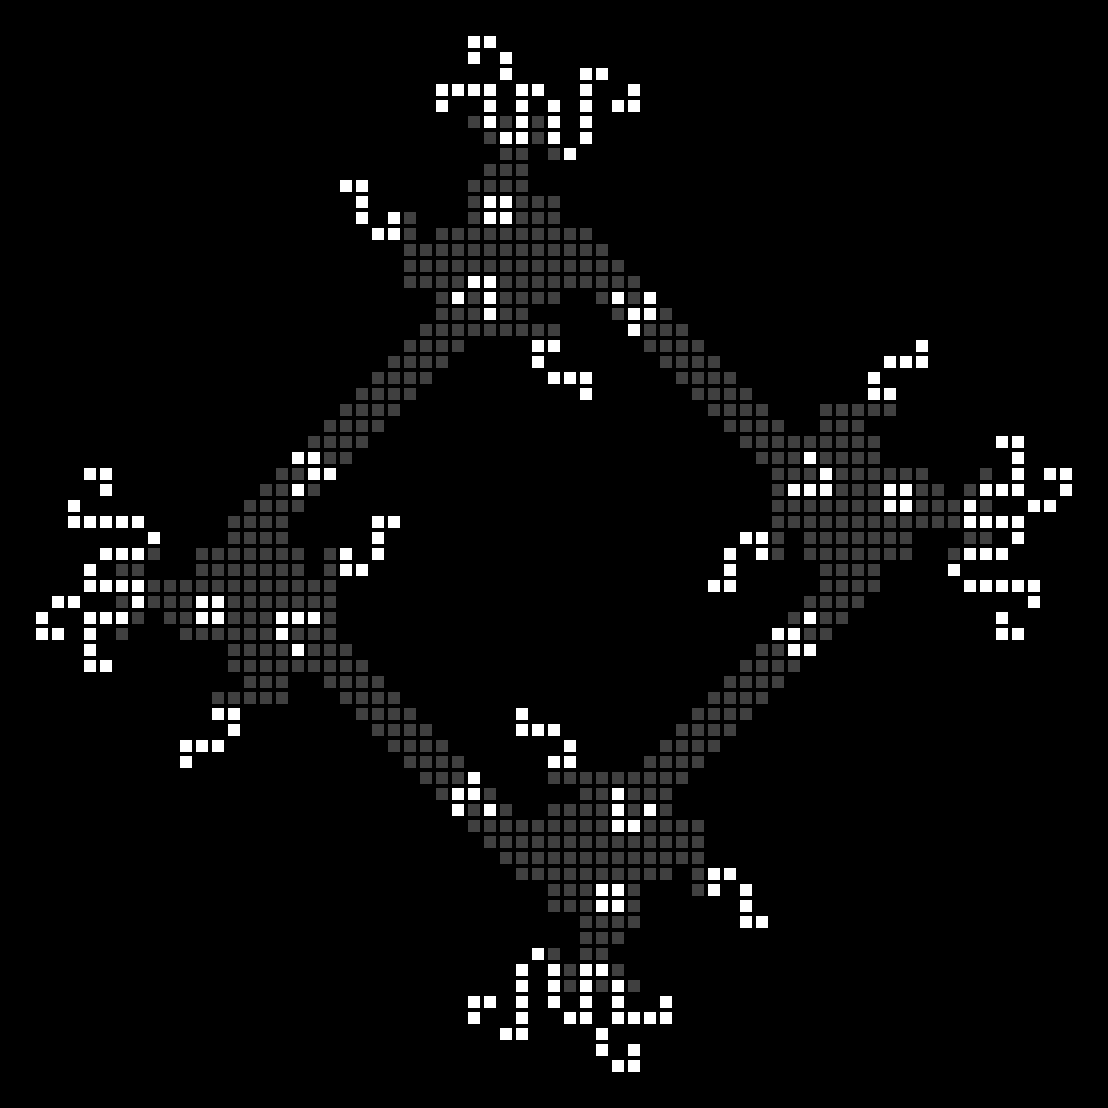
\includegraphics[width=3.2cm]{cover/glider_loop.png}}};
\draw[black,ultra thick,rounded corners=1.6pt] (-1.6,0) rectangle (1.6,-3.2);

\draw[black!20,line width=8pt,rounded corners=1.6pt] (1.76,-3.36) rectangle (4.96,-6.56); % middle right
\node[inner sep=0pt] (pi_calc) at (3.36,-4.96) {\embedlink{pi_calc}{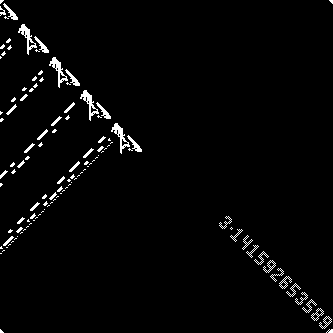
\includegraphics[width=3.2cm]{cover/pi_calc.png}}};
\draw[black,ultra thick,rounded corners=1.6pt] (1.76,-3.36) rectangle (4.96,-6.56); % middle right

\draw[black!20,line width=8pt,rounded corners=1.6pt] (1.76,-6.72) rectangle (4.96,-9.92); % bottom right
\node[inner sep=0pt] (gosper) at (3.36,-8.32) {\embedlink{gosper_glider_gun}{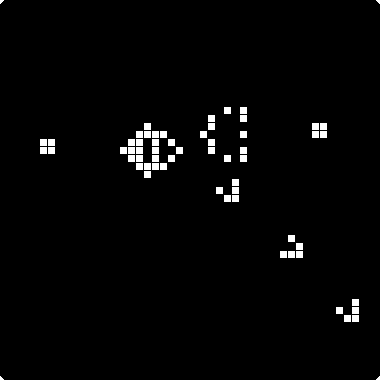
\includegraphics[width=3.2cm]{cover/gosper.png}}};
\draw[black,ultra thick,rounded corners=1.6pt] (1.76,-6.72) rectangle (4.96,-9.92); % bottom right

\draw[black!20,line width=8pt,rounded corners=1.6pt] (-1.6,-6.72) rectangle (1.6,-9.92); % bottom center
\node[inner sep=0pt] (copperhead) at (0,-8.32) {\embedlink{copperhead}{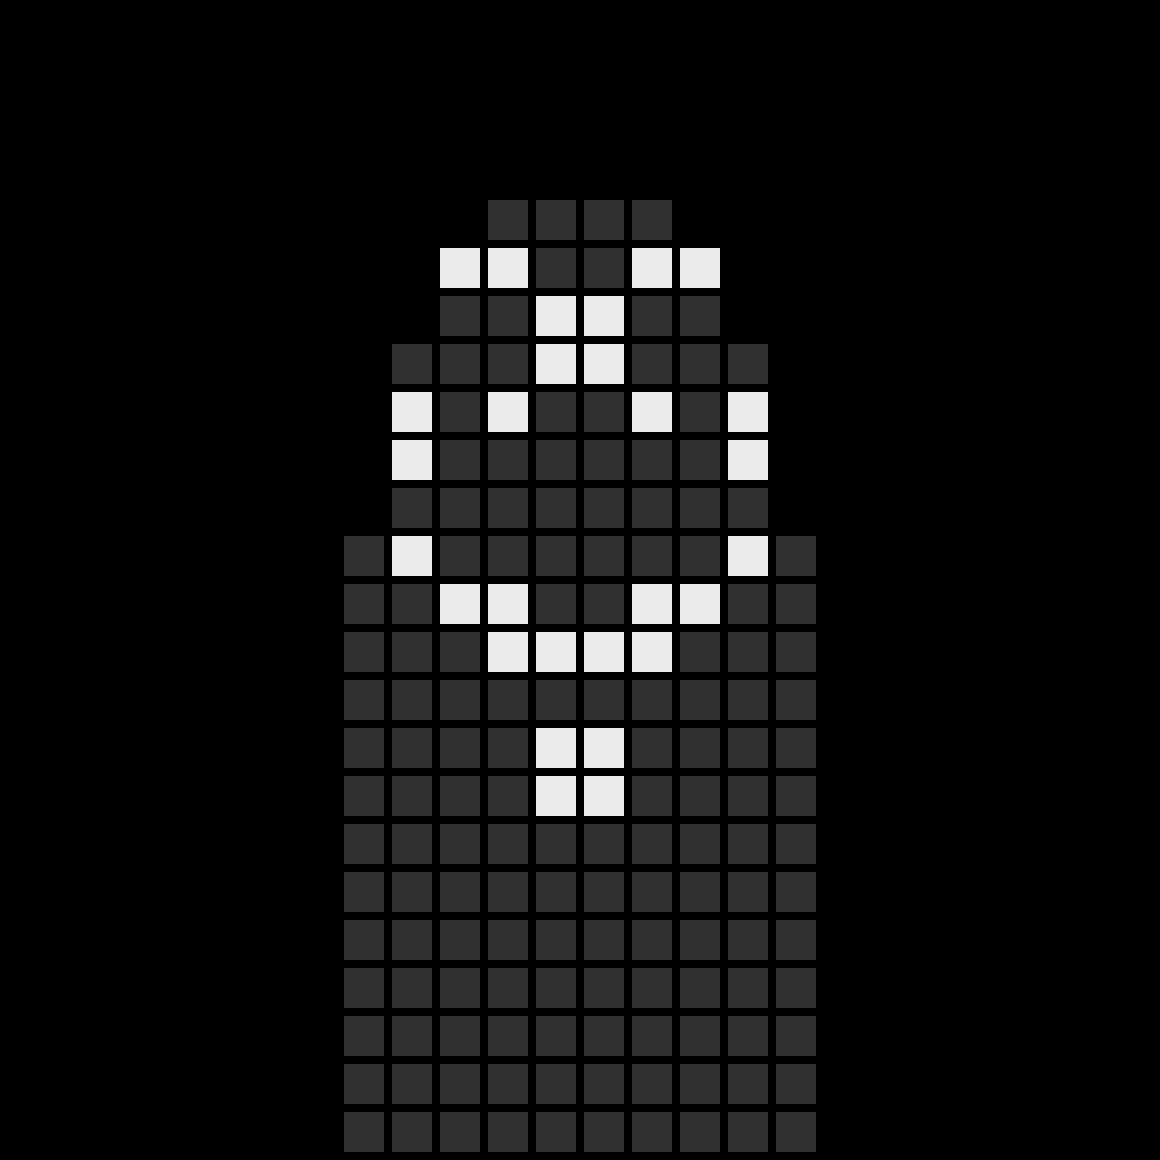
\includegraphics[width=3.2cm]{cover/copperhead.png}}};
\draw[black,ultra thick,rounded corners=1.6pt] (-1.6,-6.72) rectangle (1.6,-9.92); % bottom center

\draw[black!20,line width=8pt,rounded corners=1.6pt] (-4.96,-6.72) rectangle (-1.76,-9.92); % bottom left
\node[inner sep=0pt] (herschel) at (-3.36,-8.32) {\embedlink{herschel_track}{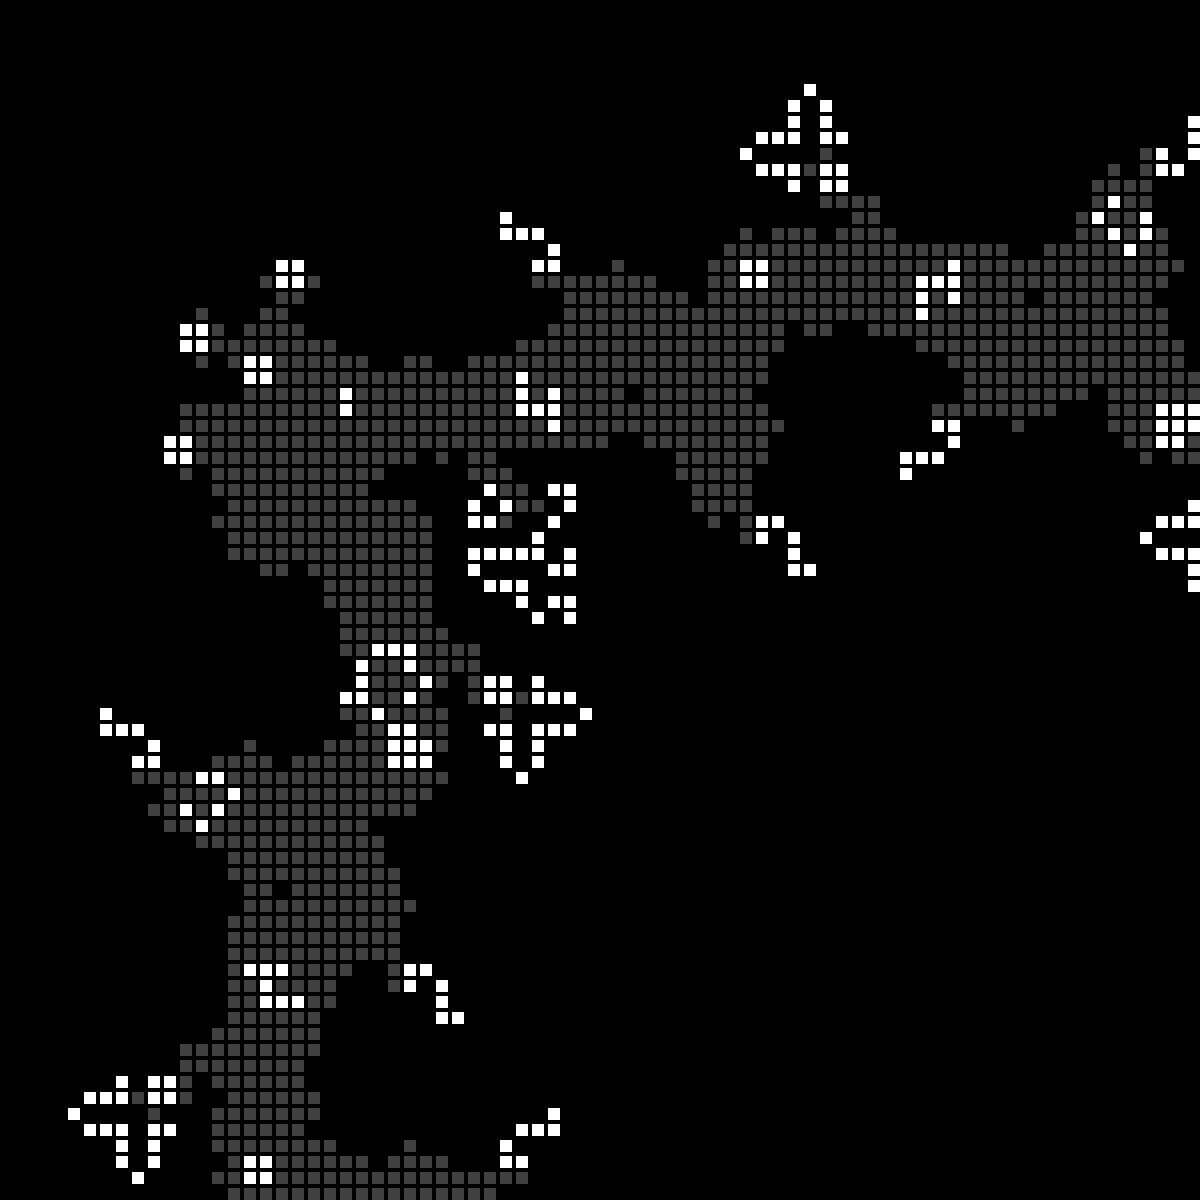
\includegraphics[width=3.2cm]{cover/herschel.png}}};
\draw[black,ultra thick,rounded corners=1.6pt] (-4.96,-6.72) rectangle (-1.76,-9.92); % bottom left
\end{tikzpicture}

\vspace*{5.55in}\textbf{\textsf{{\fontsize{16}{40}\selectfont Nathaniel Johnston} $\quad$ and $\quad$ {\fontsize{16}{40}\selectfont Dave Greene}}}
\vfill
\endgroup
\newpage
\fi

%----------------------------------------------------------------------------------------
%	COPYRIGHT PAGE
%----------------------------------------------------------------------------------------

~\vfill
\thispagestyle{empty}

\noindent Copyright \copyright\ 2022 Nathaniel Johnston and Dave Greene\\ % Copyright notice

% \noindent \textsc{Published by Publisher}\\ % 

\noindent \textsc{conwaylife.com/book}\\[0.2cm] % URL

\noindent 
\includegraphics[width=4cm]{images/isbn.pdf}



\clearpage

% DEDICATION
\vspace*{1.5in}
\begin{center}
	\textbf{\large To John Horton Conway}\\For giving us 50 years of Life.
\end{center}



%----------------------------------------------------------------------------------------
%	TABLE OF CONTENTS
%----------------------------------------------------------------------------------------

%\usechapterimagefalse % If you don't want to include a chapter image, use this to toggle images off - it can be enabled later with \usechapterimagetrue

\chapterimage{cover/toc.jpg} % Table of contents heading image

\setcounter{tocdepth}{1}
\pagestyle{empty} % No headers

\tableofcontents % Print the table of contents itself

\cleardoublepage % Forces the first chapter to start on an odd page so it's on the right

\pagestyle{fancy} % Print headers again


% The Preface section needs a custom title-line header so it doesn't start with "Chapter 0."
\renewcommand{\chaptermark}[1]{\markboth{\sffamily\normalsize\bfseries Preface}{}} % Chapter text font settings


\chapterimage{cover/preface.jpg} % Preface heading image
\renewcommand{\chapterfolder}{preface/}
\chapter{Wstęp}


\section*{Cel książki}\addcontentsline{toc}{section}{Cel książki}

W tej książce zapewniamy wprowadzenie do Gry w Życie Conwaya, matematyki kryjącej się za nią, oraz metod użytych do stworzenia wielu z jej najciekawszych wzorów. Wiele wzorów-``cegiełek'' (zwłaszcza w pierwszych czterech rozdziałach książki) zostało znalezionych za pomocą brutalnej siły lub innymi sposobami przez komputer, i nie będziemy się rozwodzić na temat detali implementacyjnych owych wyszukiwań. Jednak od tamtego miejsca staramy się przeprowadzić czytelnika przez procesy myślowe i pomysły potrzebne do połączenia tych wzorów w bardziej interesujące i złożone konstrukcje.

Chociaż przeważnie książka podąża zgodnie z historią Gry w Życie, to \emph{nie} jest to jednak jej główny cel. Jest to raczej efekt uboczny faktu, większość najnowszych odkryć bazuje na obiektach i technikach rozwiniętych wcześniej. Celem książki jest odarcie Gry w Życie z jej tajemnic poprzez rozkładanie złożonych obiektów na osobne części możliwe do zrozumienia pojedynczo.


\section*{Grupa docelowa}\addcontentsline{toc}{section}{Grupa docelowa}

Mimo że ta książka nie ma żadnych formalnych wymagań matematycznych bądź informatycznych, jest ona skierowana do poziomu studenta pierwszego roku studiów licencjackich. Niektóre tematy z poziomu liceum jak logarytmy, funkcja ''podłoga'' $f(x) = \lfloor x \rfloor$ do zaokrąglania w dół, reprezentacja dwójkowa liczb naturalnych czy notacja sumowania jak $\Sigma_{k=1}^n k^2$ do dodawania liczb, są używane często i bez większych wyjaśnień. Najbardziej zaawansowaną matematyczną maszynerią jakiej będziemy używać będzie prawdopodobnie mnożenia matryc $2 \times 2$ w Sekcji~\ref{sec:pi_calc} (ale tylko górnych trójkątnych matryc $2 \times 2$, w dodatku z podanym wzorem na mnożenie matryc).

Jest również oczekiwane podstawowe rozumienie, jak działają dowody matematyczne i programowanie komputerów. To jest, oczekujemy od czytelnika pewnego poziomu dojrzałości matematycznej i informatycznej, lecz bez specjalistycznej wiedzy na żaden z tych tematów. W całej książce udowadniamy proste twierdzenia na temat Gry w Życie. Te dowody nie używają żadnych specjalistycznych technik dowodzenia ani nie wymagają od czytelnika żadnej specyficznej wiedzy matematycznej na poziomie uniwersytetu, tylko wymagają od czytelnika żeby był w stanie podążać za logicznym rozumowaniem. Podobnie, wprowadzimy język programowania do budowania programów komputerowych z obwodów z GwŻ w Rozdziale~\ref{chp:universal_computation}, żeby materiał był prostszy do opanowania jeżeli czytelnik zetknął się wcześniej z programowaniem.

Nieco bardziej zaawansowane elementy matematyki z jakich korzystamy są streszczone w Dodatku~\ref{app:math}, chociaż są one z reguły wprowadzone również w tekście głównym, zresztą jest potrzebne tylko ich powierzchowne zrozumienie. Używamy największych wspólnych dzielników, najmniejszych wspólnych wielokrotności i tożsamości B\'ezouta przy omawianiu okresów oscylatorów w Rozdziale~\ref{chp:oscillators}, zatem wprowadzamy te narzędzia w Dodatku~\ref{sec:gcd}. Nieskończone ciągi pojawiają się na krótko pod koniec Rozdziału~\ref{chp:periodic_circuitry} i w Sekcji~\ref{sec:pi_calc}, ale nie oczekujemy od czytelników jakiejś wiedzy na ten temat ani znajomości problemów ze zbieżnością. Wreszcie, użyjemy notacji dużego $\Theta$ do omówienia wielkości i tempa wzrostu wzorów w Sekcjach~\ref{sec:large_glider_guns}, \ref{sec:irreg_guns} i~\ref{sec:Osqrtlogt}, zatem ten koncept jest wyjaśniony w Dodatku~\ref{sec:bigO}.


\section*{How to Use}\addcontentsline{toc}{section}{How to Use}

Conway's Game of Life is an extremely visual game, so this book makes very liberal use of figures throughout, particularly when new patterns or techniques for creating patterns are introduced. However, the Game of Life is best observed in motion, which makes static images in a textbook less than ideal as learning tools. In order to help present the motion of patterns a bit better, we do five things:\medskip

\begin{itemize}
	\item Figures are presented with alive cells in black and dead cells in white, but furthermore we use a gradient from blue to orange to denote cells that were alive in past generations of the pattern. Bright blue cells were just alive, whereas cells that are orange were alive in the more distant past (roughly $75$~generations or more---see Figure~\ref{fig:preface_lwss}).\bigskip

	\noindent\begin{minipage}{\linewidth}
		\centering\patternimglink{0.125}{lwss}
		\captionof{figure}{An object moving to the right with a gradient behind it indicating how long ago it was in each location. White cells were never alive, black cells are currently alive, blue cells were alive recently, and orange cells were alive long ago.}\label{fig:preface_lwss}\bigskip
	\end{minipage}
	
	\item If we really wish to emphasize what a pattern looks like in different generations, all generations of interest will be displayed, along with arrows that specify how many generations have passed. For example, if we want to clarify exactly what the pattern in Figure~\ref{fig:preface_lwss} does as it moves from left to right, we might display it as in Figure~\ref{fig:preface_lwss_2}.\bigskip
	
	\noindent\begin{minipage}{\linewidth}
		\centering\patternlink{lwss}{\vcenteredhbox{\patternimg{0.125}{lwss_1}} \vcenteredhbox{\genarrow{1}} \vcenteredhbox{\patternimg{0.125}{lwss_2}} \vcenteredhbox{\genarrow{1}} \vcenteredhbox{\patternimg{0.125}{lwss_3}} \vcenteredhbox{\genarrow{1}} \vcenteredhbox{\patternimg{0.125}{lwss_4}} \vcenteredhbox{\genarrow{1}} \vcenteredhbox{\patternimg{0.125}{lwss_5}}}
		\captionof{figure}{The same object as in Figure~\ref{fig:preface_lwss}, but displayed in a more explicit fashion. This image shows how the pattern changes every time 1 generation elapses.}\label{fig:preface_lwss_2}\bigskip
	\end{minipage}

	\item We use colors to highlight various pieces of patterns, and we maintain a consistent coloring scheme throughout the book. Light pastel colors like aqua, magenta, light green, yellow, and light orange are used to highlight \emph{around} objects---cells in these colors are dead, and they indicate a region in the Life plane consisting of cells that all serve some common purpose or logically make up one ``object'' (see Figure~\ref{fig:preface_p15_gun}). On the other hand, darker colors like dark green, dark orange, and dark red are used to highlight certain live cells. Dark green is typically used to highlight the input to some reaction, while dark orange is typically used for the output of the reaction (see Figure~\ref{fig:preface_fx77_p5_eat}).\bigskip
	
	\noindent\begin{minipage}{\linewidth}
		\centering
		\begin{minipage}[b]{0.56\textwidth}
			\centering
			\patternimg{0.11755364806}{p15_gun}
			\captionof{figure}{A glider gun made up of several different component reactions that are highlighted in different colors. In particular, gliders are created by a gun highlighted in \bgbox{magentaback}{magenta}, lightweight spaceships are created by guns highlighted in \bgbox{aquaback}{aqua} and \bgbox{yellowback2}{yellow}, and those lightweight spaceships are merged into the original glider stream by oscillators highlighted in \bgbox{orangeback2}{light orange}.}\label{fig:preface_p15_gun}
		\end{minipage}\hfill
		\begin{minipage}[b]{0.4\textwidth}
			\centering
			\patternimg{0.11}{fx77_p5_eat}
			\captionof{figure}{A \bgbox{greenback}{dark green} Herschel comes in from the left and creates the \bgbox{orangeback}{dark orange} Herschel on the right. Cells highlighted in blue are constantly changing due to being part of an oscillator, whereas cells that are light orange are usually dead, except when the Herschel passes through.}\label{fig:preface_fx77_p5_eat}
		\end{minipage}\bigskip
	\end{minipage}
	
	\item In the electronic version of this book, almost every figure is actually a clickable link that will open a text file containing RLE or Macrocell code for the displayed \ifdefined\FORPRINTING pattern.\else pattern (go ahead, click on any of the figures above, or even one of the five images on the cover page).\fi This code can be copy and pasted into Life simulation software like Golly (\httpurl{golly.sourceforge.net}) so that it can be explored and manipulated.\footnote{For an explanation of how RLE or Macrocell code works, see \httpsurl{conwaylife.com/wiki/Run_Length_Encoded} or \httpsurl{conwaylife.com/wiki/Macrocell}.} Note that clicking on figures may not work in certain PDF viewers (such as the viewers built into web browsers), so we recommend using Adobe Acrobat Reader (\httpurl{get.adobe.com/reader}) to read this book digitally.\smallskip
	
	\item RLE, LifeHistory, or Macrocell codes for all of the patterns displayed in the book are also available at the book's website (\httpsurl{conwaylife.com/book}). Furthermore, the patterns can be viewed and manipulated right on that website as well via any modern web browser, without downloading any additional software.\medskip
\end{itemize}


\subsection*{Exercises}

We strongly encourage the reader to work through this book's many exercises that can be found at the end of each chapter. For this reason, it is extremely important to either download Life software or use the book's website to view and edit patterns while making your way through the book---Life is meant to be played, not just watched, and many of the exercises simply cannot be solved without the assistance of Life simulation software.

Roughly half of the exercises are marked with an asterisk ($\ast$), which means that they have a solution provided in Appendix~\ref{chp:solutions}. Exercises also begin with a numeric difficulty estimate on a scale of 1 to 5, displayed within square brackets like \probdiff{3} or \probdiff{5}. Difficulty-1 exercises follow fairly immediately from the relevant definitions and results in the text, up to difficulty-4 exercises that involve either an extensive and delicate calculation, or a complicated multi-step construction. Difficulty-5 exercises are more like projects that could take a day or so of work to complete.


\section*{Acknowledgments}\addcontentsline{toc}{section}{Acknowledgments}

The authors are indebted to dozens of people who opened the world of Conway's Game of Life to them. Rather than acknowledging the people who discovered the reactions and patterns that we discuss here, they are credited in footnotes and figures throughout the book.

We extend thanks to Adam P.~Goucher for numerous contributions to the writing of this book, especially in Chapter~\ref{chp:0e0p}. Thanks to Nicolay Beluchenko, Oscar Cunningham, Steven Eker, Hartmut Holzwart, Tanner Jacobi, Daniel Mouscher, Mark Niemiec, David Raucci, Michael Simkin, Satoshi Tanaka, and Kalan Warusa, as well as ``AlephAlpha'', ``Chris857'', ``dani'', ``Hdjensofjfnen'', ``Ian07'', and many other ConwayLife.com forum users, for helpful conversations and corrections. Thanks to Andrew Trevorrow and Tomas Rokicki for creating the open-source cross-platform cellular automaton editor and simulator Golly (\httpurl{golly.sourceforge.net}), without which many of the patterns discussed in this book would not have been discovered. Thanks to Chris Rowett for creating LifeViewer (\httpsurl{lazyslug.com/lifeviewer}), which is used on this book's website (\httpsurl{conwaylife.com/book}) to display patterns and make them interactive. Thanks to Velimir Gayevskiy and Mathias Legrand for the \emph{Legrand Orange Book} LaTeX template from \httpurl{LaTeXTemplates.com}.

Finally, the authors would like to thank their wives Kathryn and Melanie for tolerating them during their years of mental absence glued to this book, and their parents for encouraging them to care about both learning and teaching. Many thanks also to Mount Allison University for giving the first author the academic freedom to pursue a project like this one.
% Note about license of Legrand template: https://latex.org/forum/viewtopic.php?f=59&t=30823&p=104225#p104225



\mainmatter


% Restore the standard chapter title-line header
\renewcommand{\chaptermark}[1]{\markboth{\sffamily\normalsize\bfseries\chaptername\ \thechapter.\ #1}{}} % Chapter text font settings


%----------------------------------------------------------------------------------------
%	PART 1: CLASSICAL TOPICS
%----------------------------------------------------------------------------------------

\part{Classical Topics}


%%%%%%%%%%%%%%%%%%%%%%%%%%%%%%%%%%%%%%%%%%%%%%%%%%%%%%%%%%%%%%%%%%%%%%%%%
%%   CHAPTER: EARLY LIFE
%%%%%%%%%%%%%%%%%%%%%%%%%%%%%%%%%%%%%%%%%%%%%%%%%%%%%%%%%%%%%%%%%%%%%%%%%

\renewcommand{\chapterfolder}{early_life/}
\chapterimage{cover/early_life} % Chapter heading image
\chapter{Early Life}


\vspace*{-0.4in}
\epigraph{I used to feel guilty in Cambridge that I spent all day playing games, while I was supposed to be doing mathematics. \\ Then . . . I realized that playing games \emph{is} math.}{John H. Conway}
\vspace*{0.4in}


\noindent Conway's Game of Life\footnote{Named for its inventor, John H. Conway.} is a process that takes place on an infinite square grid, where each square can be in one of two states: \emph{alive} or \emph{dead}\index{alive}\index{dead} (depicted via black and white squares, respectively, in this book). The squares (which we typically call \emph{cells})\index{cell} then evolve in discrete timesteps (called \emph{generations} or \emph{ticks})\index{generation}\index{tick} according to the following two rules:\smallskip

\begin{itemize}
	\item If a cell is alive, it survives to the next generation if it has 2 or 3 live neighbors; otherwise it dies.\smallskip
	
	\item If a cell is dead, it comes to life in the next generation if it has exactly 3 live neighbors; otherwise it stays dead.\smallskip
\end{itemize}

We note that these rules are applied to every square in the grid simultaneously, and a ``neighbor'' in these rules refers to any of the 8 cells that it touches either along a side or at a corner, as in Figure~\ref{fig:neighborhood}. As an example of how these rules work, consider what happens to the straight line of 4 alive cells depicted in Figure~\ref{fig:first_example}. The leftmost and rightmost cells in the line both only have one live neighbor, so they die, while the two central cells above and below the line each have exactly 3 live neighbors, so they come to life. This leaves us with a $3 \times 2$ rectangle of live cells, so we say that the line of 4 live cells is a \emph{parent}\index{parent} of the $3 \times 2$ rectangle of live cells, or equivalently that the $3 \times 2$ rectangle is a \emph{child}\index{child} of the line of 4 cells. We then apply the evolution rules again: this time, the two central cells in the rectangle are overpopulated and die, while the dead cells to their immediate left and right have exactly 3 live neighbors and thus come to life.

\begin{figure}[!htb]
	\centering
	\begin{minipage}[b]{0.38\textwidth}
		\centering
		\patternimg{0.125}{neighborhood}
		\caption{A live cell (in black) in the middle and its 8 neighbors (in \bgbox{yellowback2}{yellow}).}\label{fig:neighborhood}
	\end{minipage}\hfill
	\begin{minipage}[b]{0.58\textwidth}
		\centering
		\embedlink{first_example}{\vcenteredhbox{\patternimg{0.125}{first_example_0}} \vcenteredhbox{\genarrow{1}} \vcenteredhbox{\patternimg{0.125}{first_example_1}} \vcenteredhbox{\genarrow{1}} \vcenteredhbox{\patternimg{0.125}{first_example_2}}}
		\caption{A line of four alive cells takes two generations to evolve into a stable object called a \emph{beehive}\index{beehive}. The $3 \times 2$ object in the middle is sometimes called a \emph{pre-beehive}.}\label{fig:first_example}\index{pre-beehive}
	\end{minipage}
\end{figure}

After this point, if we apply the evolution rule again, nothing changes; each of the live cells have 2 live neighbors and thus live to the next generation, and no dead cell has 3 live neighbors, so they all stay dead. A pattern like this that remains unchanged from one generation to the next is called a \emph{still life}.\index{still life}

As we saw in this example, there was no input on our part once the pattern started evolving: we just applied the game's rules and passively watched what happened from one generation to the next. Instead, the ``game'' in Life is the challenge of finding new and interesting patterns that evolve in unique and unexpected ways, and that is what this book is about. We will see patterns that move back and forth periodically between a finite number of different configurations, patterns that move through the Life grid over time, and patterns that create an infinitely-growing family of other patterns. We will collide patterns with each other to create more complicated patterns, which we will then erase with even more patterns. We will construct logical circuitry with Life objects that allow us to simulate arbitrary computation within the Life universe, and we will construct patterns that do remarkable things like list the prime numbers or print out the decimal digits of $\pi$. And all of this will work simply based the two simple life and death rules we described earlier.

This all leads to a very natural question: why those rules? Why not have a dead cell come to life only in the case that it has exactly 4~live neighbors? Why not have a live cell stay alive if it has exactly 1, 2, 4, or 7 live neighbors? Indeed, there are $2^{18} = 262,144$ distinct rules that can be constructed simply by specifying different numbers of live and dead neighbors that lead to a cell staying alive or coming to life. However, the following three properties make Life special (but by no means unique):\smallskip

\begin{itemize}
	\item Its rules are \emph{simple}. For example, having a live cell stay alive if it has exactly 2 or 3 live neighbors is a more ``natural'' rule than having a live cell stay alive if it has exactly 1, 2, 4, or 7 live neighbors. This can be justified a bit by arguing that, to model something like a biological system, a cell should die of overcrowding if it has ``too many'' neighbors (e.g., since there won't be enough resources to support all of the live cells), and it should die of isolation if it has ``too few'' neighbors. The exact threshold for ``too many'' and ``too few'' is debatable, but pinned down at least somewhat by the next point.\smallskip
	
	\item It is \emph{chaotic}. Many rules (e.g., almost any rule in which a cell is born when it has 2 live neighbors) cause far too many births for anything to stabilize, so it is almost impossible for us to construct interesting objects. On the other hand, most rules in which cells are \emph{not} born when they have $3$ (or fewer) live neighbors typically lead to patterns dying off extremely quickly. Life strikes a good balance of patterns typically staying alive but not overtaking the entire grid.\smallskip
	
	\item It is \emph{historical}. This is perhaps a bit of an unsatisfying reason, but part of the interest in Life simply comes from the fact that historically it is the most well-studied rule, and it is fun to see how far we can push one very well-studied rule, rather than dividing our attention and making moderate progress on multiple rules.\smallskip
\end{itemize}

Nonetheless, other rules are sometimes studied as well, and for brevity they are typically described using a \emph{rulestring}\index{rulestring} of the form Bx/Sy, where we replace ``x'' by all numbers of live neighbors that lead to the \textbf{b}irth of a dead cell, and we replace ``y'' by all numbers of live neighbors that lead to the \textbf{s}urvival of a live cell. For example, the Game of Life is described by the rulestring B3/S23. We will comment on other rules from time to time (especially in Chapter~\ref{chp:self_support_spaceships}), typically to highlight how they contrast with Life.

There are also many more exotic ways to change the Game of Life beyond just changing the numbers of neighbors that cause cells to be alive. For example, we could have considered a \emph{neighbor}\index{neighbor} of a cell to only be one of the 4 cells that shares one of its sides as in Figure~\ref{fig:vn_neighborhood}, not just a corner (this 4-cell neighborhood is called the \emph{von Neumann neighborhood}\index{von Neumann neighborhood}, whereas the 8-cell neighborhood used by Life is called the \emph{Moore neighborhood}\index{Moore neighborhood}). We could have considered a hexagonal grid instead of a square one, or a 1D or 3D grid instead of a 2D one. We could have constructed the game in such a way that not only the number of live neighbors matters, but also their relative positions---such rules are known as \emph{isotropic rules}\index{isotropic rules}. These are all potentially interesting modifications to make, and they fall under the general umbrella of \emph{cellular automata},\index{cellular automata} but we will not consider them any further in this book. Instead, as we emphasize one final time, our goal is to take the Game of Life cellular automaton itself and push it to its farthest limits.

\begin{figure}[!htb]
	\centering
	\patternimg{0.125}{vn_neighborhood}
	\caption{A live cell (in black) in the middle and the 4 cells in its von Neumann neighborhood (in \bgbox{yellowback2}{yellow}).}\label{fig:vn_neighborhood}
\end{figure}


%%%%%%%%%%%%%%%%%%%%%%%%%%%%%%%%%%%%%%%%%%%%%%%%%%%%%%%%%%%%%%%%%%%%%%%%%
%%   SECTION: OUR FIRST TECHNIQUE: RANDOM FUMBLING
%%%%%%%%%%%%%%%%%%%%%%%%%%%%%%%%%%%%%%%%%%%%%%%%%%%%%%%%%%%%%%%%%%%%%%%%%
\section{Our First Technique: Random Fumbling}\label{sec:fumbling}

There are three main techniques used to construct objects in Life that behave in interesting and unusual ways:\smallskip

\begin{enumerate}
	\item[1)] We can write a computer program that searches for patterns with particular properties;\smallskip
	
	\item[2)] we can combine different already-known objects in such a way as to create new composite objects; or\smallskip
	
	\item[3)] we can put some random garbage on the Life board and evolve it, with the hope that something interesting pops out.\smallskip
\end{enumerate}

Option~(1) typically requires a fair bit of effort, as well as some knowledge of what exactly it is that we're searching for. Similarly, option~(2) is not yet possible for us since we are just starting out with Life and do not yet know of any objects that can be combined in an interesting way. We thus start with the extremely not clever option~(3): we try evolving a bunch of random patterns and see what is left of them after their chaos dies down.\footnote{This is not only \emph{our} approach to getting started with Life, but was also the historical approach: many of the patterns found in the first year or two of Life were found just by evolving many small configurations and looking at the results.} Our first example is presented in Figure~\ref{fig:random_1}, which is a random assortment of live cells that takes $116$~generations before stabilizing into several distinct objects. Random starting configurations like this one are sometimes called \emph{soup}\index{soup}, and the objects that they leave behind are called \emph{ash}\index{ash}.\footnote{The term ``ash'' refers to the fact that it is what is left after a pattern stops ``burning''.}

\begin{figure}[!htb]
	\centering\embedlink{random_1}{\vcenteredhbox{\patternimg{0.12}{random_1}} \vcenteredhbox{\genarrow{116}} \vcenteredhbox{\patternimg{0.085}{random_1_evolved}}}
	\caption{Evolving random junk is a decent way to find some small patterns to get us started in Life. The debris on the right introduces us to several still lifes, our first \emph{oscillator}, and the \emph{glider}.}\label{fig:random_1}
\end{figure}

In the ash, we see the beehive that we were introduced to earlier, as well as three other still lifes (i.e., patterns that do not change from one generation to the next). We also see an object called the \emph{blinker}\index{blinker} that rotates itself by 90 degrees every generation. Patterns like this one, which cycle between finitely many different configurations, are called \emph{oscillators}\index{oscillator}, and the configurations that they take on in individual generations are called \emph{phases}\index{phase}. The most exotic object that we see in the ash is the one that is traveling by itself toward the top-right corner of the Life plane. An object that moves through the plane on its own is called a \emph{spaceship}\index{spaceship}, and this particular one is called the \emph{glider}\index{glider}.

Of course, there is nothing remotely special about the particular random configuration that we started with; we could generate other random starting configurations and see what types of ash pop out of them as well. In fact, Life is so chaotic and unpredictable that we could just change a single cell of the first configuration that we used, and we will likely get a completely different set of ash. Indeed, Figure~\ref{fig:random_2} demonstrates the drastic change that can often be made by altering just one cell in a pattern: by just changing one cell from alive to dead, we have made a new pattern that takes almost 3,000 generations to stabilize and results in ash that has over 20 times as many live cells. This new ash also has three additional still lifes in it that were not present in the previous ash. A summary of the ash objects we have seen so far is given in Figure~\ref{fig:first_objects}.

\begin{figure}[!ht]
	\centering\embedlink{random_2}{\vcenteredhbox{\centering\vcenteredhbox{\begin{tikzpicture}[scale=1.2, every node/.style={transform shape}]%
			\node[inner sep=0pt,anchor=south west] at (0,0) {\patternimg{0.1}{random_2}};
			\draw[white,line width=3pt,opacity=0.5](1.314,0.965) circle (0.165);
			\draw[redback2,line width=1pt](1.314,0.965) circle (0.165);
			\end{tikzpicture}}} \vcenteredhbox{\color{black}{$\xrightarrow{\text{\clock{0}{21} 2901}}$}} \vcenteredhbox{\gridbox{0.5pt}{\patternimg{0.08}{random_2_evolved}}}}
	\caption{Changing just a single cell (circled on the left in \bgbox{redback}{red}) from alive to dead in our random starting configuration causes its evolution to become completely different. It now takes over 25 times as long to stabilize and its ash contains three new types of still lifes (ponds, ships, and loaves).}\label{fig:random_2}
\end{figure}

Still lifes, oscillators, and spaceships are the three most basic types of objects that we will study in Life, and they form the building blocks of all of the more complicated patterns that we will construct. At this point though, there are some natural questions that we can ask about them. For example, we already saw the blinker, which oscillates back and forth between $2$ phases every $2$ generations. Do there exist oscillators that take longer to return to their original configuration? In other words, do there exist oscillators with \emph{period}\index{period} larger than~$2$?

\begin{figure}[!htb]
	\centering\patternimglink{0.1}{first_objects}
	\caption{From left to right: seven still lifes, called the \emph{block}, \emph{tub}, \emph{boat}, \emph{ship}, \emph{beehive}, \emph{loaf} and \emph{pond}, an oscillator called the \emph{blinker}, and a spaceship called the \emph{glider}. All of these objects frequently appear in the ash left behind by chaotic patterns.}\label{fig:first_objects}
\end{figure}

To answer this question, we simply continue not being clever: we evolve more and more random configurations of junk and record new objects that appear in the ash as we find them. Most of the new objects that we will find by doing this are additional still lifes, but new oscillators crop up from time to time as well. For example, the oscillator depicted in Figure~\ref{fig:pulsar}, which is called the \emph{pulsar}\index{pulsar} and has period~$3$, appears rather frequently in random ash for its size.

\begin{figure}[!htb]
	\centering
	\embedlink{pulsar}{\vcenteredhbox{\patternimg{0.1}{pulsar_1}} \vcenteredhbox{\genarrow{1}} \vcenteredhbox{\patternimg{0.1}{pulsar_2}} \vcenteredhbox{\genarrow{1}} \vcenteredhbox{\patternimg{0.1}{pulsar_3}} \vcenteredhbox{\genarrow{1}} \vcenteredhbox{\patternimg{0.1}{pulsar_1}}}
	\caption{A period~3 oscillator called the \emph{pulsar}.}\label{fig:pulsar}
\end{figure}

Some other oscillators that appear reasonably often in random ash are depicted in Figure~\ref{fig:random_oscillators}. Of particular note is the \emph{pentadecathlon}\index{pentadecathlon}, which has a surprisingly large period of~15. This oscillator behaves somewhat differently than the other ones we have seen, as it pulsates and changes in size as it moves through its period---a property that will be very useful for us later on.

\begin{figure}[!htb]
	\centering\patternimglink{0.1}{random_oscillators}
	\caption{From left to right: three oscillators with period~2, called \emph{toad}\index{toad}, \emph{beacon}\index{beacon} and \emph{clock}\index{clock}, and a period~15 oscillator called \emph{pentadecathlon}.}\label{fig:random_oscillators}
\end{figure}

In the process of finding these oscillators, it is extremely likely that we will have also come across some other commonly-occurring objects, such as the \emph{lightweight spaceship}\index{lightweight!spaceship} (or \emph{LWSS}\index{LWSS|see {lightweight spaceship}} for short) depicted in Figure~\ref{fig:lwss}. This is another spaceship, but this one moves orthogonally (i.e., directly north, south, east, or west), unlike the glider, which moves diagonally.

\begin{figure}[!htb]
	\centering\embedlink{lwss}{\vcenteredhbox{\patternimg{0.1}{lwss_1}} \vcenteredhbox{\genarrow{1}} \vcenteredhbox{\patternimg{0.1}{lwss_2}} \vcenteredhbox{\genarrow{1}} \vcenteredhbox{\patternimg{0.1}{lwss_3}} \vcenteredhbox{\genarrow{1}} \vcenteredhbox{\patternimg{0.1}{lwss_4}} \vcenteredhbox{\genarrow{1}} \vcenteredhbox{\patternimg{0.1}{lwss_5}}}
	\caption{The \emph{lightweight spaceship}, which has period~4 and moves orthogonally to the right by $2$ cells every $4$ generations.}\label{fig:lwss}
\end{figure}

Slightly more rare than the lightweight spaceship are the \emph{middleweight spaceship}\index{middleweight!spaceship} (or \emph{MWSS}\index{MWSS|see {middleweight spaceship}}) and the \emph{heavyweight spaceship}\index{heavyweight!spaceship} (or \emph{HWSS}\index{HWSS|see {heavyweight spaceship}}),\footnote{In keeping with the ``\_\_\_\_weight spaceship'' naming convention, the glider was sometimes called the \emph{featherweight spaceship}\index{featherweight spaceship|see {glider}} in the early days of Life, though this name is very rarely used now.} displayed in Figure~\ref{fig:lwss_mwss_hwss}. There are a handful of other objects that a lucky Life enthusiast might see while evolving random junk, but for the most part these are the ``standard'' naturally-occurring objects. Some examples of random soups that generate more exotic objects are presented in Exercises~\ref{exer:natural_switch_engine} and~\ref{exer:random_symmetric}.

\begin{figure}[!htb]
	\centering\patternimglink{0.1}{lwss_mwss_hwss}
	\caption{From left to right: a lightweight, middleweight, and heavyweight spaceship. They all have period~$4$ and travel to the right $2$~cells every $4$~generations.}\label{fig:lwss_mwss_hwss}
\end{figure}


%%%%%%%%%%%%%%%%%%%%%%%%%%%%%%%%%%%%%%%%%%%%%%%%%%%%%%%%%%%%%%%%%%%%%%%%%
%%   SECTION: Common Evolutionary Sequences
%%%%%%%%%%%%%%%%%%%%%%%%%%%%%%%%%%%%%%%%%%%%%%%%%%%%%%%%%%%%%%%%%%%%%%%%%
\section{Common Evolutionary Sequences}\label{sec:evolution}\index{evolution}

We have seen plenty of interesting patterns so far simply by looking at the results of running random soups until they stabilize. However, we can also learn a lot by carefully watching the evolution of soups as they happen, as not only are there commonly-occurring stable ash objects, but there are also commonly-occurring unstable objects that explode and drive the evolution of those patterns. For example, one such object is the \emph{T-tetromino}\index{T-tetromino},\footnote{A \emph{polyomino}\index{polyomino} is a pattern made up of orthogonally connected live cells, and a \emph{tetromino} is a polyomino with $4$ live cells. More generally, polyominoes with $2, 3, 4, \ldots, 8$ live cells are called \emph{dominoes}, \emph{triominoes}, \emph{tetrominoes}, \emph{pentominoes}, \emph{hexominoes}, \emph{heptominoes}, and \emph{octominoes}.} which is a $4$-cell object that appears (for example) in generations $206$, $395$, and $568$ of the evolution of the soup from Figure~\ref{fig:random_2}. This tiny object (displayed in Figure~\ref{fig:t_tetromino}) explodes into an arrangement of $4$~blinkers that is called a \emph{traffic light}.\index{traffic light} In fact, three traffic lights (and part of a fourth) can be seen in the ash of Figure~\ref{fig:random_2}, and the common T-tetromino explosion is exactly why blinkers appear in this formation so frequently.

\begin{figure}[!htb]
	\centering
	\embedlink{t_tetromino}{\vcenteredhboxfx{\patternimg{0.12}{t_tetromino_0}} \vcenteredhboxfx{\genarrow{1}} \vcenteredhboxfx{${}\!\!{}$\patternimg{0.12}{t_tetromino_1}} \vcenteredhboxfx{\genarrow{1}} \vcenteredhboxfx{\patternimg{0.1}{t_tetromino_2}} \vcenteredhboxfx{\genarrow{1}} \vcenteredhboxfx{${}\!\!\!\!{}$\patternimg{0.1}{t_tetromino_3}} \vcenteredhboxfx{\genarrow{1}} \vcenteredhboxfx{${}\!\!{}$\patternimg{0.1}{t_tetromino_4}} \vcenteredhboxfx{{} \ {}} \vcenteredhboxfx{{} \ {}}\\[0.1em]
	\vcenteredhboxfx{{\color{black}${} \ \ \ \ \cdots$}} \vcenteredhboxfx{\genarrow{1}} \vcenteredhboxfx{\patternimg{0.1}{t_tetromino_5}} \vcenteredhboxfx{\genarrow{1}} \vcenteredhboxfx{\patternimg{0.1}{t_tetromino_6}} \vcenteredhboxfx{\genarrow{1}} \vcenteredhboxfx{\patternimg{0.1}{t_tetromino_7}} \vcenteredhboxfx{\genarrow{1}} \vcenteredhboxfx{\patternimg{0.085}{t_tetromino_8}} \vcenteredhboxfx{\genarrow{1}} \vcenteredhboxfx{\patternimg{0.085}{t_tetromino_9}}}
	\caption{A \emph{T-tetromino} (top-left) takes $9$ generations to evolve into an arrangement of four blinkers called a \emph{traffic light} (bottom-right).}\label{fig:t_tetromino}
\end{figure}

The T-tetromino also illustrates how symmetry spontaneously forms within Life patterns. While it starts off with only left-right symmetry, after four generations it develops top-bottom symmetry, and then after one more generation it also develops diagonal symmetry. Since Life's rules do not care about the orientation of patterns, symmetry can never be broken once it has formed, which explains why all of the later generations of the T-tetromino also have $8$-way symmetry, and why so many of the interesting and/or stable patterns that have been found in Life are symmetric.

Another unstable object that behaves similarly is the one displayed in Figure~\ref{fig:pre_honeyfarm}, which explodes over the course of $17$~generations in order to create a commonly-occurring arrangement of $4$~beehives called a \emph{honey farm}\index{honey!farm}. Appropriately enough, the $7$-cell object that starts this evolution is called the \emph{pre-honey farm}\index{pre-honey farm} (as is any other small pattern that follows the same evolution). While only one honey farm appears in the ash in Figure~\ref{fig:random_2}, many other pre-honey farms appeared earlier (for example, at generations~$749$ and $1,159$) and were subsequently destroyed.

\begin{figure}[!htb]
	\centering
	\embedlink{pre_honeyfarm}{\vcenteredhboxfx{${}\!\!\!\!\!\!{}$\patternimg{0.12}{pre_honeyfarm_0}} \vcenteredhboxfx{\genarrow{1}} \vcenteredhboxfx{${}\!\!\!\!\!\!\!\!\!\!\!{}$\patternimg{0.12}{pre_honeyfarm_1}} \vcenteredhboxfx{\genarrow{1}} \vcenteredhboxfx{${}\!\!\!\!\!\!\!\!\!\!\!{}$\patternimg{0.12}{pre_honeyfarm_2}} \vcenteredhboxfx{\genarrow{1}} \vcenteredhboxfx{${}\!\!\!\!\!\!\!\!\!\!{}$\patternimg{0.11}{pre_honeyfarm_3}} \vcenteredhboxfx{\genarrow{1}} \vcenteredhboxfx{${}\!\!\!\!\!\!\!\!\!{}$\patternimg{0.11}{pre_honeyfarm_4}} \vcenteredhboxfx{\genarrow{1}} \vcenteredhboxfx{${}\!\!\!\!\!\!\!\!\!\!{}$\patternimg{0.105}{pre_honeyfarm_5}} \\[0.1em]
	\vcenteredhboxfx{{\color{black}${} \ \ \ \ \cdots$}} \vcenteredhboxfx{\genarrow{1}} \vcenteredhboxfx{${}\!\!\!\!\!\!\!\!{}$\patternimg{0.1}{pre_honeyfarm_6}} \vcenteredhboxfx{\genarrow{1}} \vcenteredhboxfx{${}\!\!\!\!\!\!\!\!{}$\patternimg{0.1}{pre_honeyfarm_7}} \vcenteredhboxfx{\genarrow{1}} \vcenteredhboxfx{${}\!\!\!\!\!\!\!{}$\patternimg{0.095}{pre_honeyfarm_8}} \vcenteredhboxfx{\genarrow{1}} \vcenteredhboxfx{${}\!\!\!\!\!\!{}$\patternimg{0.095}{pre_honeyfarm_9}} \vcenteredhboxfx{\genarrow{1}} \vcenteredhboxfx{${}\!\!\!\!\!\!{}$\patternimg{0.09}{pre_honeyfarm_10}} \\[0.2em]
	\vcenteredhboxfx{{\color{black}$ \ \ \ \ \cdots$}} \vcenteredhboxfx{\genarrow{1}} \vcenteredhboxfx{${}\!\!\!\!\!{}$\patternimg{0.09}{pre_honeyfarm_11}} \vcenteredhboxfx{\genarrow{1}} \vcenteredhboxfx{${}\!\!\!{}$\patternimg{0.08}{pre_honeyfarm_12}} \vcenteredhboxfx{\genarrow{1}} \vcenteredhboxfx{${}\!\!\!{}$\patternimg{0.08}{pre_honeyfarm_13}} \vcenteredhboxfx{\genarrow{1}} \vcenteredhboxfx{${}\!\!{}$\patternimg{0.075}{pre_honeyfarm_14}} \vcenteredhboxfx{\genarrow{1}} \vcenteredhboxfx{${}\!\!{}$\patternimg{0.075}{pre_honeyfarm_15}} \\[0.3em]
	\vcenteredhboxfx{{\color{black}$ \ \ \ \cdots$}} \vcenteredhboxfx{${}\!\!\!{}$\genarrow{1}} \vcenteredhboxfx{${}\!\!\!{}$\patternimg{0.075}{pre_honeyfarm_16}} \vcenteredhboxfx{\genarrow{1}} \vcenteredhboxfx{${}\!\!\!{}$\patternimg{0.075}{pre_honeyfarm_17}} \vcenteredhboxfx{\phantom{\genarrow{1}}} \vcenteredhboxfx{\phantom{\patternimg{0.08}{pre_honeyfarm_17}}} \vcenteredhboxfx{\phantom{\genarrow{1}}} \vcenteredhboxfx{\phantom{\patternimg{0.08}{pre_honeyfarm_17}}} \vcenteredhboxfx{\phantom{\genarrow{1}}} \vcenteredhboxfx{\phantom{\patternimg{0.08}{pre_honeyfarm_17}}}}
	\caption{A \emph{pre-honey farm} (top-left) takes $17$ generations to evolve into an arrangement of four beehives called a \emph{honey farm} (bottom-right).}\label{fig:pre_honeyfarm}
\end{figure}

A slightly messier explosion that is sometimes useful is the one that begins with the \emph{stairstep hexomino}\index{stairstep hexomino} displayed in Figure~\ref{fig:stairstep_hexomino}. This object takes $63$~generations to stabilize into an arrangement of four blocks called the \emph{blockade}\index{blockade}. However, since the blockade is somewhat larger than the traffic light and the honey farm, and it also takes much longer to form, it is less commonly seen in ash. For example, the stairstep hexomino can be seen at generation~$1,005$ of the evolution of the soup in Figure~\ref{fig:random_2}, but it is interfered with before the blockade can form.

\begin{figure}[!htb]
	\centering
	\embedlink{stairstep_hexomino}{\vcenteredhbox{\patternimg{0.12}{stairstep_hexomino_0}} \vcenteredhbox{\genarrow{3}}
	\vcenteredhbox{\patternimg{0.12}{stairstep_hexomino_3}} \vcenteredhbox{\genarrow{60}} \vcenteredhbox{\patternimg{0.12}{stairstep_hexomino_63}}}
	\caption{The \emph{stairstep hexomino} (left) evolves into an arrangement of four blocks called the \emph{blockade} in $63$~generations. This evolution, and any of the intermediate patterns, are often called \emph{lumps of muck}.}\label{fig:stairstep_hexomino}
\end{figure}

It is also often the case that this evolution begins with another small pattern, such as the third generation of the stairstep hexomino, rather than the stairstep hexomino itself. For this reason, this evolutionary sequence, and any of the patterns that appear during its $63$-generation explosion, are given a common name: \emph{lumps of muck}\index{lumps of muck}.

As one final example, consider the extremely common and extremely messy \emph{pi-heptomino}\index{pi-heptomino} displayed in Figure~\ref{fig:pi_heptomino}, which appears at generation~$61$ in the evolution of the soup in Figure~\ref{fig:random_1} and numerous times in the evolution of the soup in Figure~\ref{fig:random_2} (e.g., in generations $46$, $164$, $206$, $208$, $233$, $\ldots$). While it does not evolve into any particularly interesting stable objects (a rather unremarkable collection of $6$~blocks, $5$~blinkers, and $2$~ponds), it has the interesting property that it moves forward by $9$~cells after $30$ generations, while leaving behind some messy debris. While this is not quite useful by itself, it can be made useful by combining the pi-heptomino with other objects that destroy the debris before it gets in the way. By doing so, we can use the pi-heptomino to transmit a signal from one place in the Life plane to another or act like a spaceship. We will explore these ideas in Chapter~\ref{chp:stationary_circuitry} and Section~\ref{sec:caterpillar}.

\begin{figure}[!htb]
	\centering
	\embedlink{pi_heptomino}{\vcenteredhbox{\patternimg{0.125}{pi_heptomino_0}} \vcenteredhbox{\genarrow{1}}
	\vcenteredhbox{\patternimg{0.125}{pi_heptomino_1}} \vcenteredhbox{\genarrow{30}} \vcenteredhbox{\patternimg{0.1}{pi_heptomino_31}} \vcenteredhbox{\genarrow{142}} \vcenteredhbox{\patternimg{0.08}{pi_heptomino_173}}}
	\caption{The \emph{pi-heptomino} is a commonly-occurring unstable object that moves forward by $9$~cells after $30$~generations (compare the middle two patterns), but leaves behind debris that prevents it from moving ahead another $9$~cells.}\label{fig:pi_heptomino}
\end{figure}


%%%%%%%%%%%%%%%%%%%%%%%%%%%%%%%%%%%%%%%%%%%%%%%%%%%%%%%%%%%%%%%%%%%%%%%%%
%%   SECTION: THE QUEEN BEE
%%%%%%%%%%%%%%%%%%%%%%%%%%%%%%%%%%%%%%%%%%%%%%%%%%%%%%%%%%%%%%%%%%%%%%%%%
\section{The Queen Bee}\label{sec:queen_bee}\index{queen bee}

Sometimes, it is possible to ``fix'' unstable evolutionary patterns by tweaking them in some simple way, thus creating interesting objects that do not often appear naturally by themselves. Perhaps the most useful example of such a pattern is the \emph{queen bee}, which is a commonly-occurring object\footnote{For example, it appears in generation~1,185 of the soup in Figure~\ref{fig:random_2}.} that reflects itself after $15$~generations, but leaves behind a beehive in the process. It follows that after 30~generations, the queen bee is back where it started, but with an additional beehive on either side of it (see Figure~\ref{fig:queen_bee}). Shortly after 30~generations, the queen bee collides with the first beehive that it created, resulting in its self-destruction.

\begin{figure}[!htb]
	\centering\embedlink{queen_bee}{\vcenteredhbox{\patternimg{0.1}{queen_bee_0}} \vcenteredhbox{\genarrow{15}} \vcenteredhbox{\patternimg{0.1}{queen_bee_15}} \vcenteredhbox{\genarrow{15}} \vcenteredhbox{\patternimg{0.1}{queen_bee_30}}}
	\caption{A \emph{queen bee} (left) reflects itself and leaves a beehive behind every 15 generations. After doing this twice, the beehives start interfering with the queen bee, causing it to explode.}\label{fig:queen_bee}
\end{figure}

In order to prevent this self-destruction and turn the queen bee into something useful (an oscillator), we need a way to delete the beehives as they are created. Possibly the simplest way to do this is to use the reaction displayed in Figure~\ref{fig:beehive_block}, in which a block being placed next to a beehive results in the beehive being destroyed and the block surviving unharmed (we thus say that the block \emph{eats}\index{eater} the beehive\footnote{We will look at eaters in more depth in Section~\ref{sec:eaters}.}).

\begin{figure}[!htb]
	\centering
	\embedlink{beehive_block}{\vcenteredhbox{\phantom{$\cdots$ \genarrow{1}}} \vcenteredhbox{\patternimg{0.1}{beehive_block_0}} \vcenteredhbox{\genarrow{1}} \vcenteredhbox{\patternimg{0.1}{beehive_block_1}} \vcenteredhbox{\genarrow{1}} \vcenteredhbox{\patternimg{0.1}{beehive_block_2}} \vcenteredhbox{\genarrow{1}} \vcenteredhbox{\patternimg{0.1}{beehive_block_3}} \vcenteredhbox{\phantom{\genarrow{1}}} \vcenteredhbox{\phantom{\patternimg{0.1}{beehive_block_3}}} \\[0.7em]
	\vcenteredhbox{\phantom{\genarrow{1}}} \vcenteredhbox{\phantom{\patternimg{0.1}{beehive_block_3}}} \vcenteredhbox{$\cdots$ \genarrow{1}} \vcenteredhbox{\patternimg{0.1}{beehive_block_4}} \vcenteredhbox{\genarrow{1}} \vcenteredhbox{\patternimg{0.1}{beehive_block_5}} \vcenteredhbox{\genarrow{1}} \vcenteredhbox{\patternimg{0.1}{beehive_block_6}} \vcenteredhbox{\genarrow{1}} \vcenteredhbox{\patternimg{0.1}{beehive_block_7}}}
	\caption{Placing a block next to a beehive destroys the beehive in 7~generations, without permanently damaging the block.}\label{fig:beehive_block}
\end{figure}

We can now simply paste these two reactions together to create an oscillator in which a queen bee (initially facing right) creates a beehive and is reflected to the left, then a block destroys the beehive while the queen bee creates another beehive and is reflected back to the right, then a block destroys the second beehive and the whole process repeats. This period~30 oscillator is called the \emph{queen bee shuttle}\footnote{The term ``shuttle'' typically refers to oscillators in which an unstable object moves back and forth between stabilizing objects (e.g., in this case, the unstable queen bee moves back and forth between the stabilizing blocks on either side of it).}\index{queen bee!shuttle} and is displayed in Figure~\ref{fig:queen_bee_shuttle}.

\begin{figure}[!ht]
	\centering\patternimglink{0.1}{queen_bee_shuttle}
	\caption{The \emph{queen bee shuttle} is a period~30 oscillator constructed by combining the reactions in Figures~\ref{fig:queen_bee} and~\ref{fig:beehive_block}.}\label{fig:queen_bee_shuttle}
\end{figure}

The queen bee shuttle is our first example on an engineered object---a pattern that we didn't discover ``naturally'', but rather one that we specifically constructed by piecing together simpler reactions that we had observed. This is how most recent discoveries in the Game of Life have been made, and it is also the route that we will take through most of the later chapters in this book: we will combine simple patterns and reactions that we have already seen into more complicated patterns that serve a new purpose, and then we will combine those objects into even more sophisticated patterns, and so on.

The queen bee can also be stabilized by some objects other than blocks (see Exercise~\ref{exer:queen_bee_eater_1}). Perhaps the most interesting and useful way to stabilize a queen bee is to use another (very carefully positioned) queen bee. If lined up and timed just right, the queen bees bounce off of each other, and instead of each producing a beehive, their collision produces a glider. This is remarkable, since we can then place stabilizing blocks on the other side of each queen bee so as to create a pattern that oscillates at period~30, but also creates an endless stream of gliders (see Figure~\ref{fig:gosper_glider_gun}). Patterns that create glider streams are called \emph{glider guns}\index{glider!gun}, and this particular one is called the \emph{Gosper glider gun}\index{Gosper glider gun}.\footnote{Named after Bill Gosper, who found it in November~1970.} This is the first pattern that we have seen that grows indefinitely (and indeed, it was the first such pattern ever to be discovered), and we will make extensive use of it when constructing more complex objects in later chapters.\footnote{Whether or not there are finite patterns that grow arbitrarily large was one of the major open questions in the early days of Life, and this glider gun's discovery earned Gosper a \$50 reward from Conway himself.}

\begin{figure}[!htb]
	\centering\patternimglink{0.1}{gosper_glider_gun}
	\caption{The \emph{Gosper glider gun} creates a never-ending stream of gliders by bouncing two queen bees back and forth between two blocks (the object at the top-right is indeed a queen bee, just in a different phase than in the other figures).}\label{fig:gosper_glider_gun}
\end{figure}


%%%%%%%%%%%%%%%%%%%%%%%%%%%%%%%%%%%%%%%%%%%%%%%%%%%%%%%%%%%%%%%%%%%%%%%%%
%%   SECTION: THE B-HEPTOMINO AND TWIN BEES
%%%%%%%%%%%%%%%%%%%%%%%%%%%%%%%%%%%%%%%%%%%%%%%%%%%%%%%%%%%%%%%%%%%%%%%%%
\section{The B-Heptomino and Twin Bees}\label{sec:twin_bees}\index{twin bees}\index{B-heptomino}

Another commonly-occurring\footnote{For example, it occurs at generation~$106$ of the soup from Figure~\ref{fig:random_1} and generation~$210$ of the soup from Figure~\ref{fig:random_2}.} unstable pattern that is very similar in flavor to the queen bee and the pi-heptomino is the \emph{B-heptomino}. This object, like the pi-heptomino, has the interesting property that it behaves somewhat like a spaceship---after 10 generations it evolves into a copy of itself 5 cells forward, plus some extra junk behind it (see Figure~\ref{fig:b_heptomino_10}). However, it is then quickly killed by its trailing debris before it has a chance to repeat this process.

Stabilizing the B-heptomino in order to turn it into a useful object is slightly more involved than it was for the queen bee, but fortunately nature does some of the hard work for us: B-heptominoes often occur in pairs, in a configuration that is called the \emph{twin bees},\footnote{The name ``twin bees'' refers both to the fact that many of its properties and uses are completely analogous to the queen bee, and also to the fact that it is made up of two B-heptominoes, so its name can be read as ``twin Bs''.} which are displayed in Figure~\ref{fig:twin_bees}. When in pairs like this, the B-heptominoes survive longer than when on their own, and in fact they now reflect themselves, just like the queen bee did (albeit after $23$ generations instead of $15$) while leaving some junk behind in the process. Unlike the queen bee, the twin bees do not survive long enough to reflect themselves a second time, since the mess they leave behind explodes and destroys them very shortly after the first reflection.

\begin{figure}[!htb]
	\centering
	\begin{minipage}[b]{0.46\textwidth}
		\centering\embedlink{b_heptomino}{\vcenteredhbox{\patternimg{0.099}{b_heptomino}} \vcenteredhbox{\genarrow{10}} \vcenteredhbox{\patternimg{0.099}{b_heptomino_10}}}
		\caption{A \emph{B-heptomino} (depicted in \bgbox{greenback}{green} on the left) takes 10~generations to move forward by 5~cells (in \bgbox{orangeback}{orange} on the right) and create a bunch of junk behind it. The trailing junk subsequently destroys the B-heptomino, preventing it from traveling any farther.}\label{fig:b_heptomino_10}
	\end{minipage}\hfill
	\begin{minipage}[b]{0.5\textwidth}
		\centering\embedlink{twin_bees}{\vcenteredhbox{\patternimg{0.0855}{twin_bees_0}} \vcenteredhbox{\genarrow{23}} \vcenteredhbox{\patternimg{0.0855}{twin_bees_23}}}
		\caption{Twin bees reflect themselves and leave behind a chaotic mess every 23 generations (the two-cell objects in the middle of the image on the right die off in the next generation and thus have no effect).}\label{fig:twin_bees}
	\end{minipage}
\end{figure}

In order to stabilize the twin bees, we take a cue from the queen bee and try placing blocks in such a way as to eat the mess that is left behind. This works very well, and the stabilization displayed in Figure~\ref{fig:twin_bees_debris_eat} was already known in the very early days of Life.\footnote{This stabilization was found by Bill Gosper in 1971.}

\begin{figure}[!htb]
	\centering
	\embedlink{twin_bees_debris_eat}{\vcenteredhbox{\patternimg{0.09}{twin_bees_debris_eat_1}} \vcenteredhbox{\genarrow{1}} \vcenteredhbox{\patternimg{0.09}{twin_bees_debris_eat_2}} \vcenteredhbox{\genarrow{1}} \vcenteredhbox{\patternimg{0.09}{twin_bees_debris_eat_3}} \vcenteredhbox{\genarrow{1}} \vcenteredhbox{\patternimg{0.09}{twin_bees_debris_eat_4}} \vcenteredhbox{\genarrow{1}} \vcenteredhbox{\patternimg{0.09}{twin_bees_debris_eat_5}} \vcenteredhbox{\genarrow{1}} \vcenteredhbox{\patternimg{0.09}{twin_bees_debris_eat_6}}}
	\caption{Placing two blocks next to the debris left behind by twin bees destroys that debris in 5~generations, while leaving the blocks intact.}\label{fig:twin_bees_debris_eat}
\end{figure}

We now do exactly what we did with the queen bee: we place blocks on \emph{both} sides of the twin bees so that they reflect from the right to the left, their debris is destroyed, then they reflect from the left to the right, their debris is destroyed again, and then they repeat. This whole process takes $23 + 23 = 46$ generations to complete, and results in the period~46 oscillator known as the \emph{twin bees shuttle}\index{twin bees!shuttle} displayed in Figure~\ref{fig:twin_bees_shuttle}.

\begin{figure}[!htb]
	\centering\patternimglink{0.1}{twin_bees_shuttle}
	\caption{The \emph{twin bees shuttle} is a period~46 oscillator constructed by combining the reactions in Figures~\ref{fig:twin_bees} and~\ref{fig:twin_bees_debris_eat}.}\label{fig:twin_bees_shuttle}
\end{figure}

As with the queen bee, there are many other ways to stabilize the twin bees shuttle besides using two blocks on each side as in~\ref{fig:twin_bees_debris_eat}, and some of these alternate stabilizations are investigated in Exercise~\ref{exer:twin_bees_stabilize}. In fact, we can even collide two pairs of twin bees with each other to create a period~46 glider gun in almost the exact same way that we constructed the Gosper glider gun by colliding two queen bees. This new glider gun,\footnote{This gun was also found by Bill Gosper.} which we call the \emph{twin bees gun}\index{twin bees!gun},\footnote{A slight variant of this gun was originally found in 1971 and called the \emph{new gun}\index{new gun|see {twin bees gun}}, since it was the first gun to be found after the Gosper glider gun. However, this name is woefully out of date at this point.} is shown in Figure~\ref{fig:twin_bees_gun}.

\begin{figure}[!htb]
	\centering\patternimglink{0.1}{twin_bees_gun}
	\caption{The \emph{twin bees gun} is a period~$46$ glider gun that was constructed by bouncing two twin bees back and forth between each other and two stabilizing pairs of blocks. Note that the pair of objects in the middle-right are indeed twin bees, just in a different phase than the other figures.}\label{fig:twin_bees_gun}
\end{figure}


%%%%%%%%%%%%%%%%%%%%%%%%%%%%%%%%%%%%%%%%%%%%%%%%%%%%%%%%%%%%%%%%%%%%%%%%%
%%   SECTION: THE SWITCH ENGINE
%%
%%   http://conwaylife.com/forums/viewtopic.php?f=2&t=1406
%%%%%%%%%%%%%%%%%%%%%%%%%%%%%%%%%%%%%%%%%%%%%%%%%%%%%%%%%%%%%%%%%%%%%%%%%
\section{The Switch Engine}\label{sec:switch_engine}\index{switch engine}

One final commonly-occurring unstable pattern that is worth introducing at this point is the \emph{switch engine}, which is the configuration of 8 live cells displayed in Figure~\ref{fig:switch_engine}. Just like the queen bee and twin bees, the switch engine leaves behind some debris and reappears later on in its evolution (this time after 48 generations), but in a different location and orientation. However, unlike the queen bee and twin bees, the switch engine does not return to its original position after repeating this reaction. Instead, the switch engine continually moves farther and farther away from where it started, just like a spaceship.

\begin{figure}[!htb]
	\centering\embedlink{switch_engine}{\vcenteredhbox{\patternimg{0.1}{switch_engine_0}} \vcenteredhbox{\genarrow{48}} \vcenteredhbox{\patternimg{0.1}{switch_engine_48}} \vcenteredhbox{\genarrow{48}} \vcenteredhbox{\patternimg{0.1}{switch_engine_96}}}
	\caption{A \emph{switch engine} (outlined in \bgbox{aquaback}{aqua}) moves and reflects itself across the diagonal every 48 generations, but leaves behind some chaotic junk in the process. After 96 generations, the switch engine is back in its original orientation, but 8 cells northeast of where it started. The switch engine appears for the last time in generation 1,152, after repeating this entire process 12 times. The chaotic junk then finally collides with the switch engine and destroys it.}\label{fig:switch_engine}
\end{figure}

As with several other patterns that we have now explored, the switch engine will be destroyed by its debris if we do not stabilize it somehow. Because of the continued movement of the switch engine, we don't expect to be able to convert it into a stationary object like an oscillator or glider gun, like we did with the queen bee or twin bees from the previous sections, but rather we hope to turn it into some sort of ``useful'' moving object like a spaceship.

It turns out that turning it into a spaceship is actually somewhat tricky, so we defer that discussion to Section~\ref{sec:corderships}. However, there are simple ways to stabilize it into a moving object that is \emph{not} a spaceship. For example, if we place a block next to a switch engine as in Figure~\ref{fig:switch_engine_block}, then it evolves into an object called the \emph{block-laying switch engine}\index{switch engine!block-laying|see {block-laying switch engine}}\index{block-laying switch engine}---a switch engine whose debris settles down into an ever-lengthening stream of blocks (8 blocks every 288 generations).

\begin{figure}[!htb]
	\centering\embedlink{switch_engine_block}{\vcenteredhbox{\patternimg{0.125}{switch_engine_block_0}} \vcenteredhbox{\genarrow{768}} \vcenteredhbox{\patternimg{0.1}{switch_engine_block_768}}}
	\caption{A switch engine (outlined in \bgbox{aquaback}{aqua}) with a single block strategically placed next to it evolves into a \emph{block-laying switch engine}---a pattern that repeatedly lays a configuration of 8 blocks (outlined in \bgbox{yellowback2}{yellow}) every 288 generations as it moves northeast.}\label{fig:switch_engine_block}
\end{figure}

An object like this one, which moves but leaves periodic junk behind it, is called a \emph{puffer}\index{puffer}. Another puffer can be constructed from a switch engine by instead placing a block next to it as in Figure~\ref{fig:switch_engine_glider}. In this case, the pattern evolves into something called the \emph{glider-producing switch engine}\index{switch engine!glider-producing|see {glider-producing switch engine}}\index{glider-producing switch engine}, which is a switch engine that leaves behind four blinkers, three blocks, two beehives, a boat, a ship, a loaf, and a glider every 384 generations. The glider travels in the same direction as the switch engine, but because the glider travels faster (at a pace of $3$ cells every $12$ generations, versus the switch engine's $1$ cell every $12$ generations), it does not take long for it to pass the switch engine.

\begin{figure}[!htb]
	\centering\embedlink{switch_engine_glider}{\vcenteredhbox{\patternimg{0.125}{switch_engine_glider_0}} \vcenteredhbox{\color{black}{$\xrightarrow{\text{\clock{9}{37} 2016}}$}} \vcenteredhbox{\gridbox{0.5pt}{\patternimg{0.1}{switch_engine_glider_2016}}}}
	\caption{A switch engine (outlined in \bgbox{aquaback}{aqua}) with a single block strategically placed next to it can also evolve into a \emph{glider-producing switch engine}, which repeatedly lays a messy pattern of 4 blinkers, 8 still lifes, and one glider (outlined in \bgbox{yellowback2}{yellow}) every 384 generations, as it moves northeast.}\label{fig:switch_engine_glider}
\end{figure}

The block-laying and glider-producing switch engines are remarkable for the fact that, not only do they grow infinitely, but they are also ``natural'' (as opposed to engineered, like the Gosper glider gun). In fact, puffers based on switch engines are the only infinitely-growing patterns that have ever formed as a result of randomly filling some portion of the Life plane and then evolving it (see Exercise~\ref{exer:natural_switch_engine}). The ease with which these switch engine puffers appear (compared to other infinitely-growing patterns like the two glider guns we saw earlier) can be explained by noting that they have some very small predecessors, like the 12-cell objects shown in Figures~\ref{fig:switch_engine_block} and~\ref{fig:switch_engine_glider},\footnote{These 12-cell predecessors can be turned into 11-cell predecessors by simply removing a single cell from the block.} whereas glider guns require a comparatively large number of ``coordinated'' live cells to form.


%%%%%%%%%%%%%%%%%%%%%%%%%%%%%%%%%%%%%%%%%%%%%%%%%%%%%%%%%%%%%%%%%%%%%%%%%
%%   SUBSECTION: ARKS
%%%%%%%%%%%%%%%%%%%%%%%%%%%%%%%%%%%%%%%%%%%%%%%%%%%%%%%%%%%%%%%%%%%%%%%%%
\subsection{Arks}\label{sec:arks}\index{ark}

Perhaps an even more natural way to stabilize a switch engine is to use additional switch engines; after all, using a stationary object (like a block) to stabilize a moving object seems somewhat nonsensical, and only worked for us because the switch engine was able to turn the block into a moving stabilization (this is why the bottom-left corners of Figures~\ref{fig:switch_engine_block} and~\ref{fig:switch_engine_glider} are irregular: the block itself wasn't the stabilization, but rather it just reacted chaotically with the switch engine's debris in such a way that it eventually created a moving stabilization).

On the other hand, using a moving object to stabilize another moving object (or using two moving objects to stabilize each other) is a common technique that we will use repeatedly. In this particular case, any puffer created by using two switch engines is called an \emph{ark}\index{ark}, and dozens can be found just by trying different positions and phases of nearby switch engines. For example, if we place two switch engines next to each other as in Figure~\ref{fig:ark_1}, the result is an ark that leaves behind a multitude of different objects, but does so in a periodic way: the same collection of still lifes, oscillators, and gliders is created every $576$~generations, offset by $48$~cells diagonally.

\begin{figure}[!htb]
	\centering\embedlink{ark_1}{\vcenteredhbox{\patternimg{0.1}{ark_1}} \vcenteredhbox{\color{black}{$\xrightarrow{\text{\clock{4}{48} 1728}}$}} \vcenteredhbox{\gridbox{0.5pt}{\patternimg{0.1}{ark_1_1728}}}}
	\caption{Two switch engines (outlined in \bgbox{aquaback}{aqua}) can be used to stabilize each other and create an \emph{ark}. In this particular ark, the switch engines leave behind two gliders, two toads, eight blinkers, and 42 still lifes (outlined in \bgbox{yellowback2}{yellow}) every 576 generations.}\label{fig:ark_1}
\end{figure}


%%%%%%%%%%%%%%%%%%%%%%%%%%%%%%%%%%%%%%%%%%%%%%%%%%%%%%%%%%%%%%%%%%%%%%%%%
%%   SECTION: METHUSELAHS AND STABILITY
%%%%%%%%%%%%%%%%%%%%%%%%%%%%%%%%%%%%%%%%%%%%%%%%%%%%%%%%%%%%%%%%%%%%%%%%%
\section{Methuselahs and Stability}\label{sec:methuselah}\index{methuselah}

Some of the patterns that we have investigated are extremely chaotic and take a long time to stabilize,\footnote{We will see shortly that properly defining what it means for a pattern to ``stabilize'' is very troublesome, but for now it just means that the pattern has broken down into non-interacting still lifes, oscillators, and spaceships.} such as the B-heptomino and the random configuration depicted in Figure~\ref{fig:random_2}, which take $148$ and 2,901 generations to stabilize, respectively. More extreme than either of these examples is the $8$-cell switch engine, which takes 3,911 generations to stabilize---considerably longer than most other patterns with $8$ or fewer cells. It seems somewhat natural to ask how far these examples can be pushed---that is, how long can a pattern of a given size take to stabilize? A pattern that takes exceptionally long to stabilize, relative to other similarly-sized patterns, is called a \emph{methuselah}.\footnote{Named after the Biblical man Methuselah who reportedly lived the longest of any human---969 years.}

Before looking at more specific examples of methuselahs, we make it very clear up front that this definition is very imprecise: there is no completely objective way to say that some patterns are methuselahs while other patterns aren't. Instead, the classification usually takes place simply by comparing the lifespan of the pattern with the longest known lifespan of similarly-sized patterns. Here, ``size'' may refer to either the number of live cells in the pattern, or to the area of its \emph{bounding box}\index{bounding box}, which is the smallest rectangle that contains it.

No good search methods are known for finding methuselahs, so all of them have been found essentially by random guessing or exhaustive search. As an example, consider the \emph{R-pentomino}\index{R-pentomino}, which is depicted in Figure~\ref{fig:r_pentomino}. This pattern is interesting for the fact that it takes considerably longer to stabilize than any other pattern that fits with in a $3 \times 3$ bounding box, and also much longer to stabilize than any other polyomino with $5$ or fewer live cells (see Exercise~\ref{exer:pentominoes}).\footnote{However, there are 5-cell patterns that are \emph{not} polyominoes that last slightly longer, as demonstrated in Table~\ref{tab:small_methuselahs}.} The evolutionary sequence that evolves from it is also extremely important---it produces a B-heptomino (well, actually a \emph{B-heptaplet}\index{B-heptaplet} that evolves in the same way) in generation~$28$, an important object called a \emph{Herschel}\index{Herschel} in generation~$48$, and the very first glider that was ever observed in Life\footnote{First noticed by Richard~K.~Guy in 1970.} in generation~$69$.\footnote{In fact, all of the unstable objects from Section~\ref{sec:evolution} appear during the R-pentomino's evolution---see Exercise~\ref{exer:find_unstable}.}

\begin{figure}[!htb]
	\centering\embedlink{r_pentomino}{\vcenteredhbox{\patternimg{0.1}{r_pentomino}} \vcenteredhbox{\genarrow{28}} \vcenteredhbox{\patternimg{0.1}{r_pentomino_28}} \vcenteredhbox{\genarrow{20}} \vcenteredhbox{\patternimg{0.1}{r_pentomino_48}} \vcenteredhbox{\color{black}{$\xrightarrow{\text{\clock{5}{35} 1055}}$}} \vcenteredhbox{\gridbox{0.5pt}{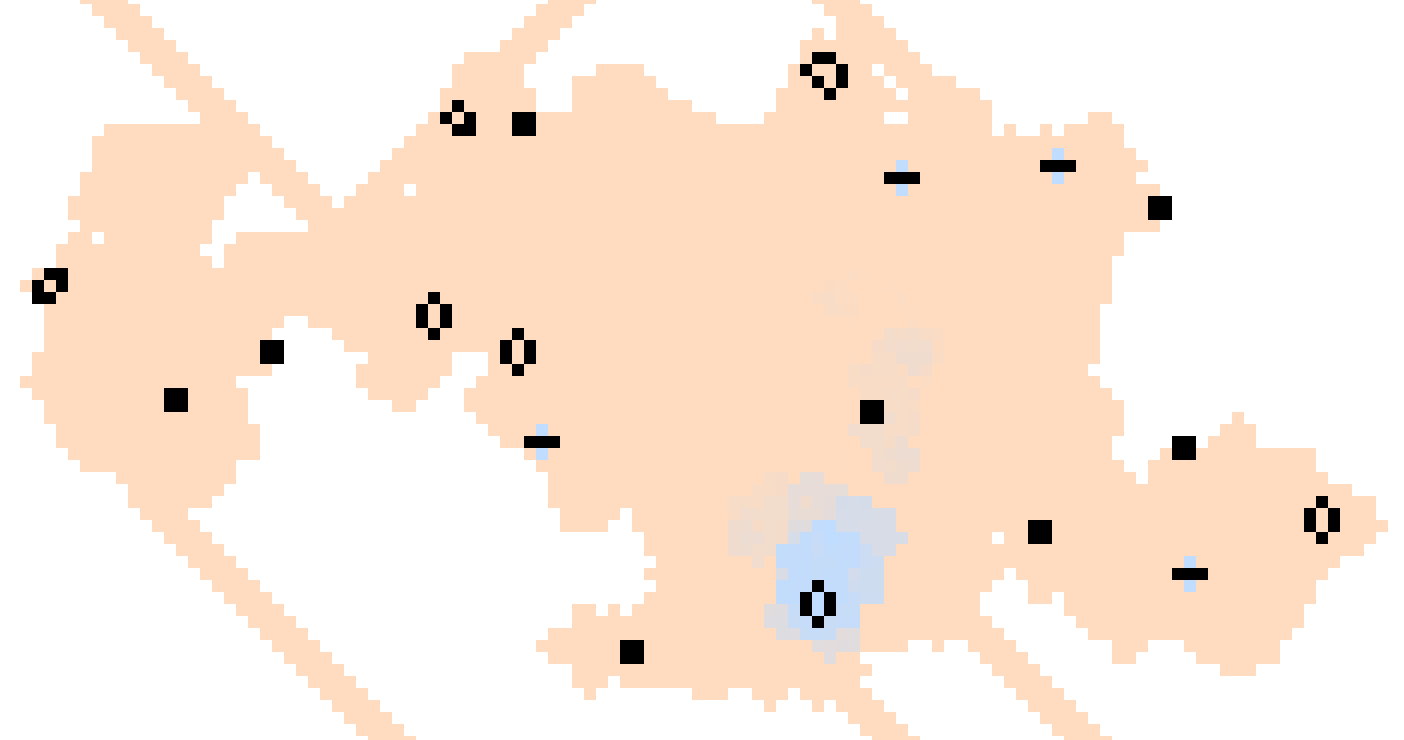
\includegraphics[scale=0.1]{early_life/r_pentomino_evolved}}}}
	\caption{An R-pentomino takes 1,103 generations to stabilize---much longer than any other polyomino with 5 or fewer cells. Along the way, it produces numerous other important patterns such as the \emph{B-heptaplet} highlighted in \bgbox{aquaback}{aqua} and the \emph{Herschel} highlighted in \bgbox{magentaback}{magenta}.}\label{fig:r_pentomino}
\end{figure}

We could similarly ask what the longest-lived pattern with $n$ cells for $n = 6, 7, 8, \ldots$ are. The longest-lived such patterns that are known are summarized in Table~\ref{tab:small_methuselahs}, as long as we restrict our attention only to patterns with reasonably small bounding boxes (which of course is subjective). However, these patterns are only known to be optimal for $n \leq 9$;\footnote{Exhaustive computer searches for methuselahs with $n \leq 9$ cells were carried out by Paul Callahan in 1997, Tomas Rokicki in 2005, and Nick Gotts in 2019.} the longest-lasting known $10$-cell methuselah in a small bounding box was not found until 2019.

\begin{table}[!htb]\vspace*{0.05in}
	\begin{center}		
		\begin{tabular}{Sc Sc Sl Sc}
			\toprule
			Cells & Methuselah & Name & Lifespan \\\midrule
			\specialcell{5} & \specialcell{\patternimglink{0.1}{5_cell_methuselahs}} & \specialcell{R-pentomino grandparents} & \specialcell{1,105} \\

			\rowcolor{gray!20} \specialcell{6} & \specialcell{\patternimglink{0.1}{6_cell_methuselahs}} & \specialcell{R-pentomino great-great-great grandparents} & \specialcell{1,108} \\
			
			\specialcell{7} & \specialcell{\patternimglink{0.1}{acorn}} & \specialcell{acorn\index{acorn}} & \specialcell{5,206} \\

			\rowcolor{gray!20} \specialcell{8} & \specialcell{\patternimglink{0.1}{7468M}} & -- & \specialcell{7,468} \\
			
			\specialcell{9} & \specialcell{\patternimglink{0.1}{bunnies}} & \specialcell{bunnies 9\index{bunnies!9}} & \specialcell{17,410} \\ % bunnies 9
			
			\rowcolor{gray!20} \specialcell{10} & \specialcell{\patternimglink{0.1}{bunnies_10b}} & \specialcell{bunnies 10b\index{bunnies!10b}} & \specialcell{17,431} \\ % bunnies 10b

			\specialcell{11} & \specialcell{\patternimglink{0.1}{23334M}} & -- & \specialcell{23,334} \\
			
			\rowcolor{gray!20} \specialcell{12} & \specialcell{\patternimglink{0.1}{methuselah_12}} & -- & \specialcell{23,801} \\
			
			\specialcell{13} & \specialcell{\patternimglink{0.1}{lidka}} & \specialcell{Lidka\index{Lidka}} & \specialcell{29,126} \\\bottomrule
		\end{tabular}
		\caption{The longest-lived known methuselahs with 5--13 cells. The methuselahs with 7 or fewer cells were all known by no later than 1971: the R-pentomino relatives were fairly well-known, so their exact discoverer is difficult to pin down, but the acorn was found by Charles Corderman. The methuselah with 8 cells was found by Tomas Rokicki in 2005, bunnies~9 was found by Paul Callahan in 1997, bunnies 10b was found by Nick Gotts in November 2019, and the 11-, 12-, and 13-cell methuselahs were found by Simon Ekström in May 2016, February 2017, and March 2017, respectively.}\label{tab:small_methuselahs}
	\end{center}
\end{table}

To highlight the difficulty of defining methuselahs in a rigorous way, note that there are 8- and 9-cell patterns that can be made to have lifespans as long as we like, since we can just aim a glider at a far away blinker or a block. However, these somewhat trivial examples can be avoided by requiring that a methuselah have a suitably small bounding box (which also rules out $8$-cell methuselahs like the one displayed in Exercise~\ref{exer:8cell_methuselah}). If we go this route and focus on the bounding box of a pattern, rather than its number of cells, then we find patterns like the one displayed in Figure~\ref{fig:47575m},\footnote{Found by Adam P.~Goucher in February 2019.} which fits within a $16 \times 16$ bounding box and has a lifespan of 47,575 generations, which is longer than any other known pattern of this size.

Another potential problem that arises when discussing methuselahs and stability comes from the fact that we already saw patterns with just 12 cells that grow indefinitely: the block-laying and glider-producing switch engines\footnote{This can easily be reduced to 11 cells by removing one of the cells in the block in either pattern.} of Section~\ref{sec:switch_engine}. This is not too difficult to take care of: even though these patterns grow forever, they do so in a regular and predictable way. For example, to know what a block-laying switch engine looks like in generation 5,000,000, we don't actually need to evolve it 5,000,000 times: we could simply move the switch engine the correct number of spaces to the northeast and paste a trail of blocks behind it. We could thus say, for example, that the block-laying switch engine stabilizes once it enters the periodic portion of its evolution where it repeatedly lays $8$ blocks every $288$ generations.

These problems might seem simple enough to overcome by tweaking our definitions carefully, but they are just the tip of the iceberg when it comes to what can go wrong when trying to rigorously define methuselahs and what it means for a pattern to stabilize. As yet another example, consider the remarkable 16-cell pattern\footnote{Found by Nick Gotts in 2005.} depicted in Figure~\ref{fig:ark_736692}, which takes 736,692 generations to stabilize.

\begin{figure}[!htb]
	\centering
	\begin{minipage}[b]{0.4\textwidth}
		\centering\patternimglink{0.11}{47575m}
		\caption{A methuselah that fits within a $16 \times 16$ bounding box and takes 47,575 generations to stabilize.}\label{fig:47575m}
	\end{minipage}\hfill
	\begin{minipage}[b]{0.56\textwidth}
		\centering\patternimglink{0.09}{ark_736692}
		\caption{A 16-cell pattern that takes a whopping 736,692 generations to stabilize. The $8$-cell objects at the top-right and bottom-left individually are just predecessors of the switch engine, so this pattern is an ark.}\label{fig:ark_736692}
	\end{minipage}
\end{figure}

The ``problem'' with this pattern is that its non-stabilization is rather artificial; it evolves into adjacent block-laying and glider-producing switch engines, which interact in such a way as to fire a glider backward toward some debris every 2,304 generations. Every time this backward glider hits the debris, it transforms it into something slightly different and unpredictable. This process repeats more than 250 times before it breaks down and a glider destroys the debris enough that future gliders pass right through without touching it at all. However, by this point the pattern has been growing for over 700,000 generations into the huge mess shown in Figure~\ref{fig:ark_736692_stabilized}.

\begin{figure}[!htb]
	\centering\begin{tikzpicture}%
		\node[inner sep=0pt,anchor=south west] (zoom1) at (-1,1) {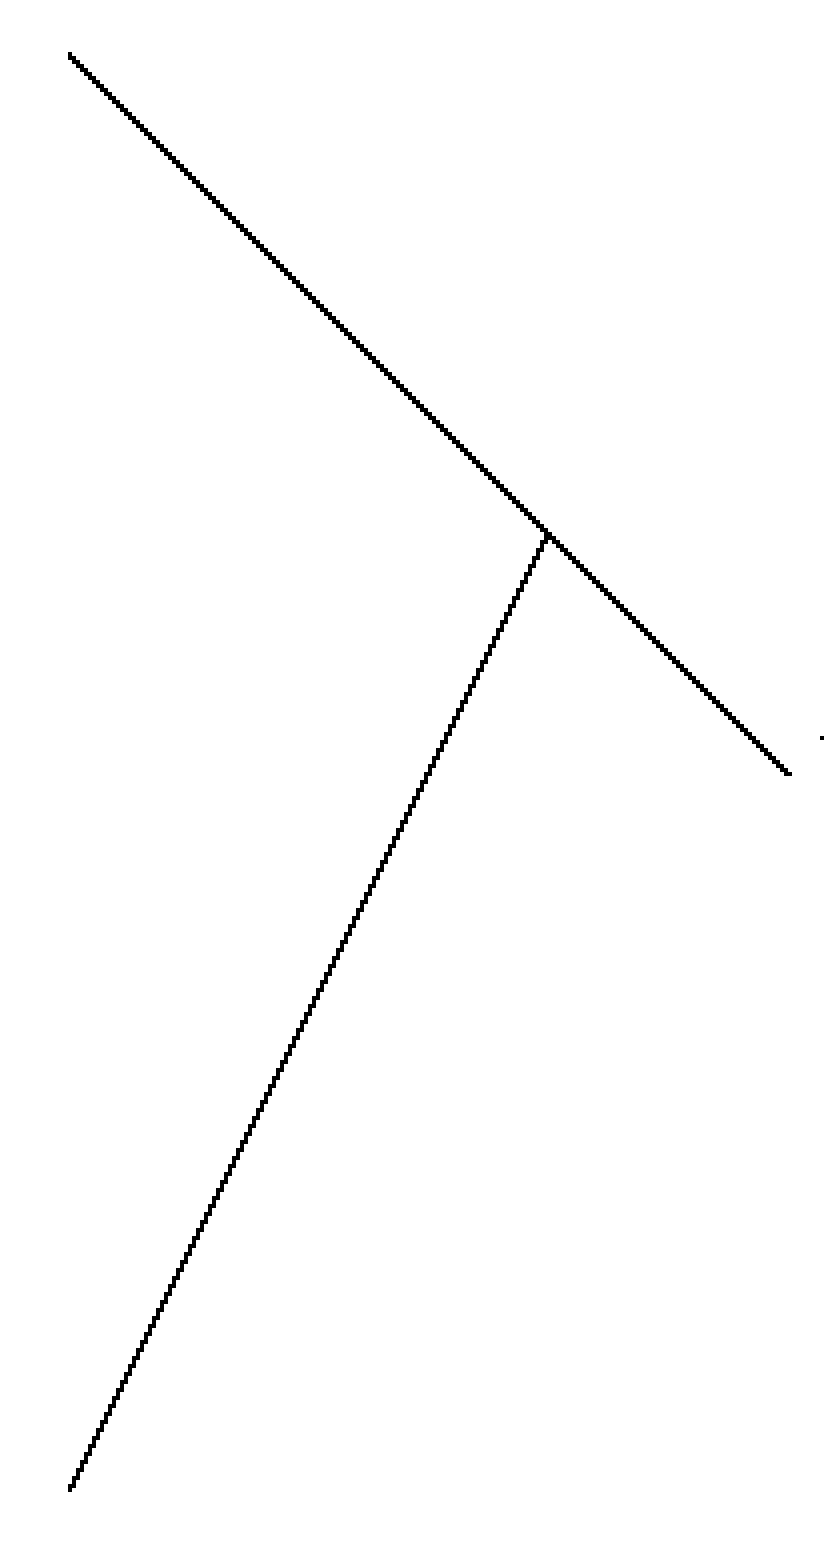
\includegraphics[width=2.8cm]{early_life/ark_736692_1.png}};
		\draw[gridgray,line width=0.75pt] (-1,1) rectangle (1.8,6.147);
		
		% ZOOM BOX 1
		\path[draw,gridgray,line width=0.5pt] (1.653,3.803) -- (11.9,8.1) -- cycle;
		\path[draw,gridgray,line width=0.5pt] (1.653,3.55) -- (11.9,0) -- cycle;

		\path[fill,white,opacity=0.85,line width=0pt] (1.4,3.55) -- (3.8,0) -- (11.9,0) -- (11.9,8.1) -- (3.8,8.1) -- (1.4,3.803) -- (1.653,3.803) -- (1.653,3.55) -- cycle;
		\draw[gridgray,line width=0.5pt] (1.4,3.55) rectangle (1.653,3.803);
	
		\path[draw,gridgray,line width=0.5pt] (1.4,3.803) -- (3.8,8.1) -- cycle;
		\path[draw,gridgray,line width=0.5pt] (1.4,3.55) -- (3.8,0) -- cycle;
		
		\node[inner sep=0pt] (zoom1_32x) at (2.8,3.7) {
\includegraphics[width=0.3cm]{mag.png} 32x};
		% END ZOOM BOX 1
		
		\node[inner sep=0pt,anchor=south west] (zoom2) at (3.8,0) {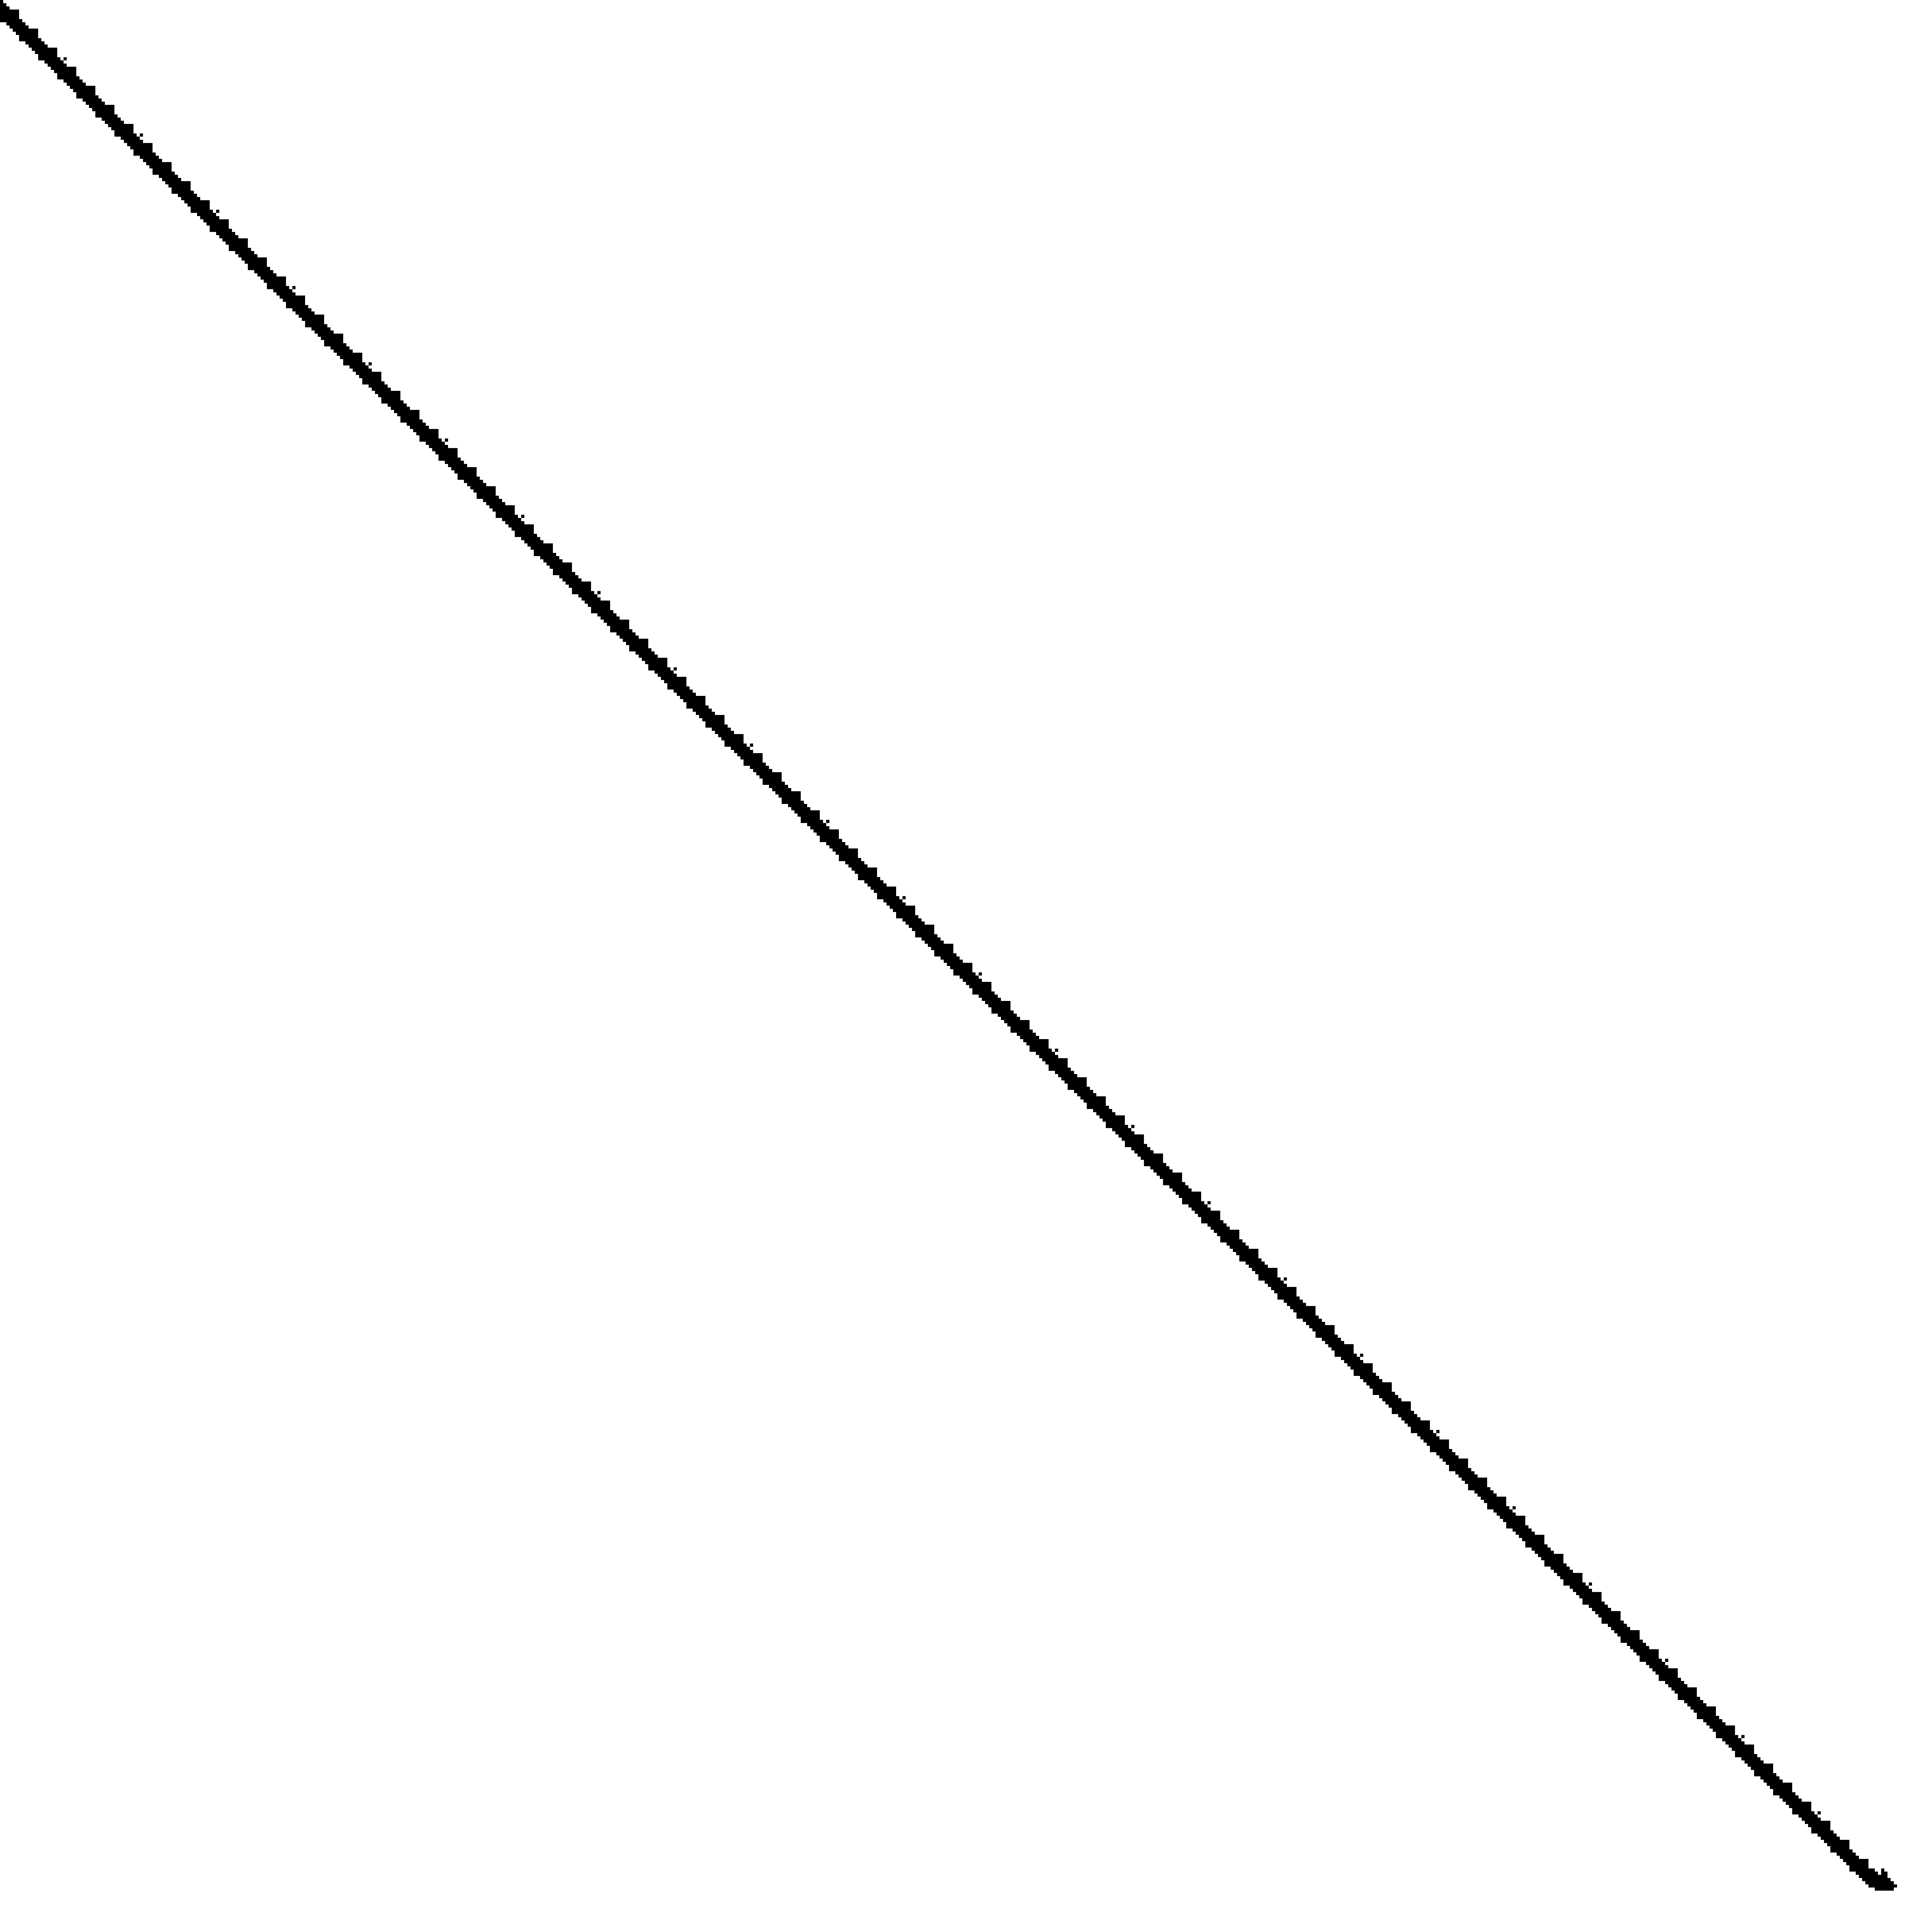
\includegraphics[width=8.1cm]{early_life/ark_736692_2.png}};
		\draw[gridgray,line width=0.75pt] (3.8,0) rectangle (11.9,8.1);
		
		% ZOOM BOX 2
		\path[draw,gridgray,line width=0.5pt] (11.51,0.14) -- (2,-9) -- cycle;
		
		\path[fill,white,opacity=0.85,line width=0pt] (11.51,0.367) -- (2,-1.75) -- (2,-9) -- (10.53,-9) -- (11.777,0.14) -- (11.51,0.14) -- cycle;
		\draw[gridgray,line width=0.5pt] (11.51,0.14) rectangle (11.777,0.367);
		
		\path[draw,gridgray,line width=0.5pt] (11.51,0.367) -- (2,-1.75) -- cycle;
		\path[draw,gridgray,line width=0.5pt] (11.777,0.367) -- (10.53,-1.75) -- cycle;
		\path[draw,gridgray,line width=0.5pt] (11.777,0.14) -- (10.53,-9) -- cycle;
		
		\node[inner sep=0pt] (zoom1_32x) at (9,-1) {
\includegraphics[width=0.3cm]{mag.png} 32x};
		% END ZOOM BOX 2

		\node[inner sep=0pt,anchor=south west] (zoom3) at (2,-9) {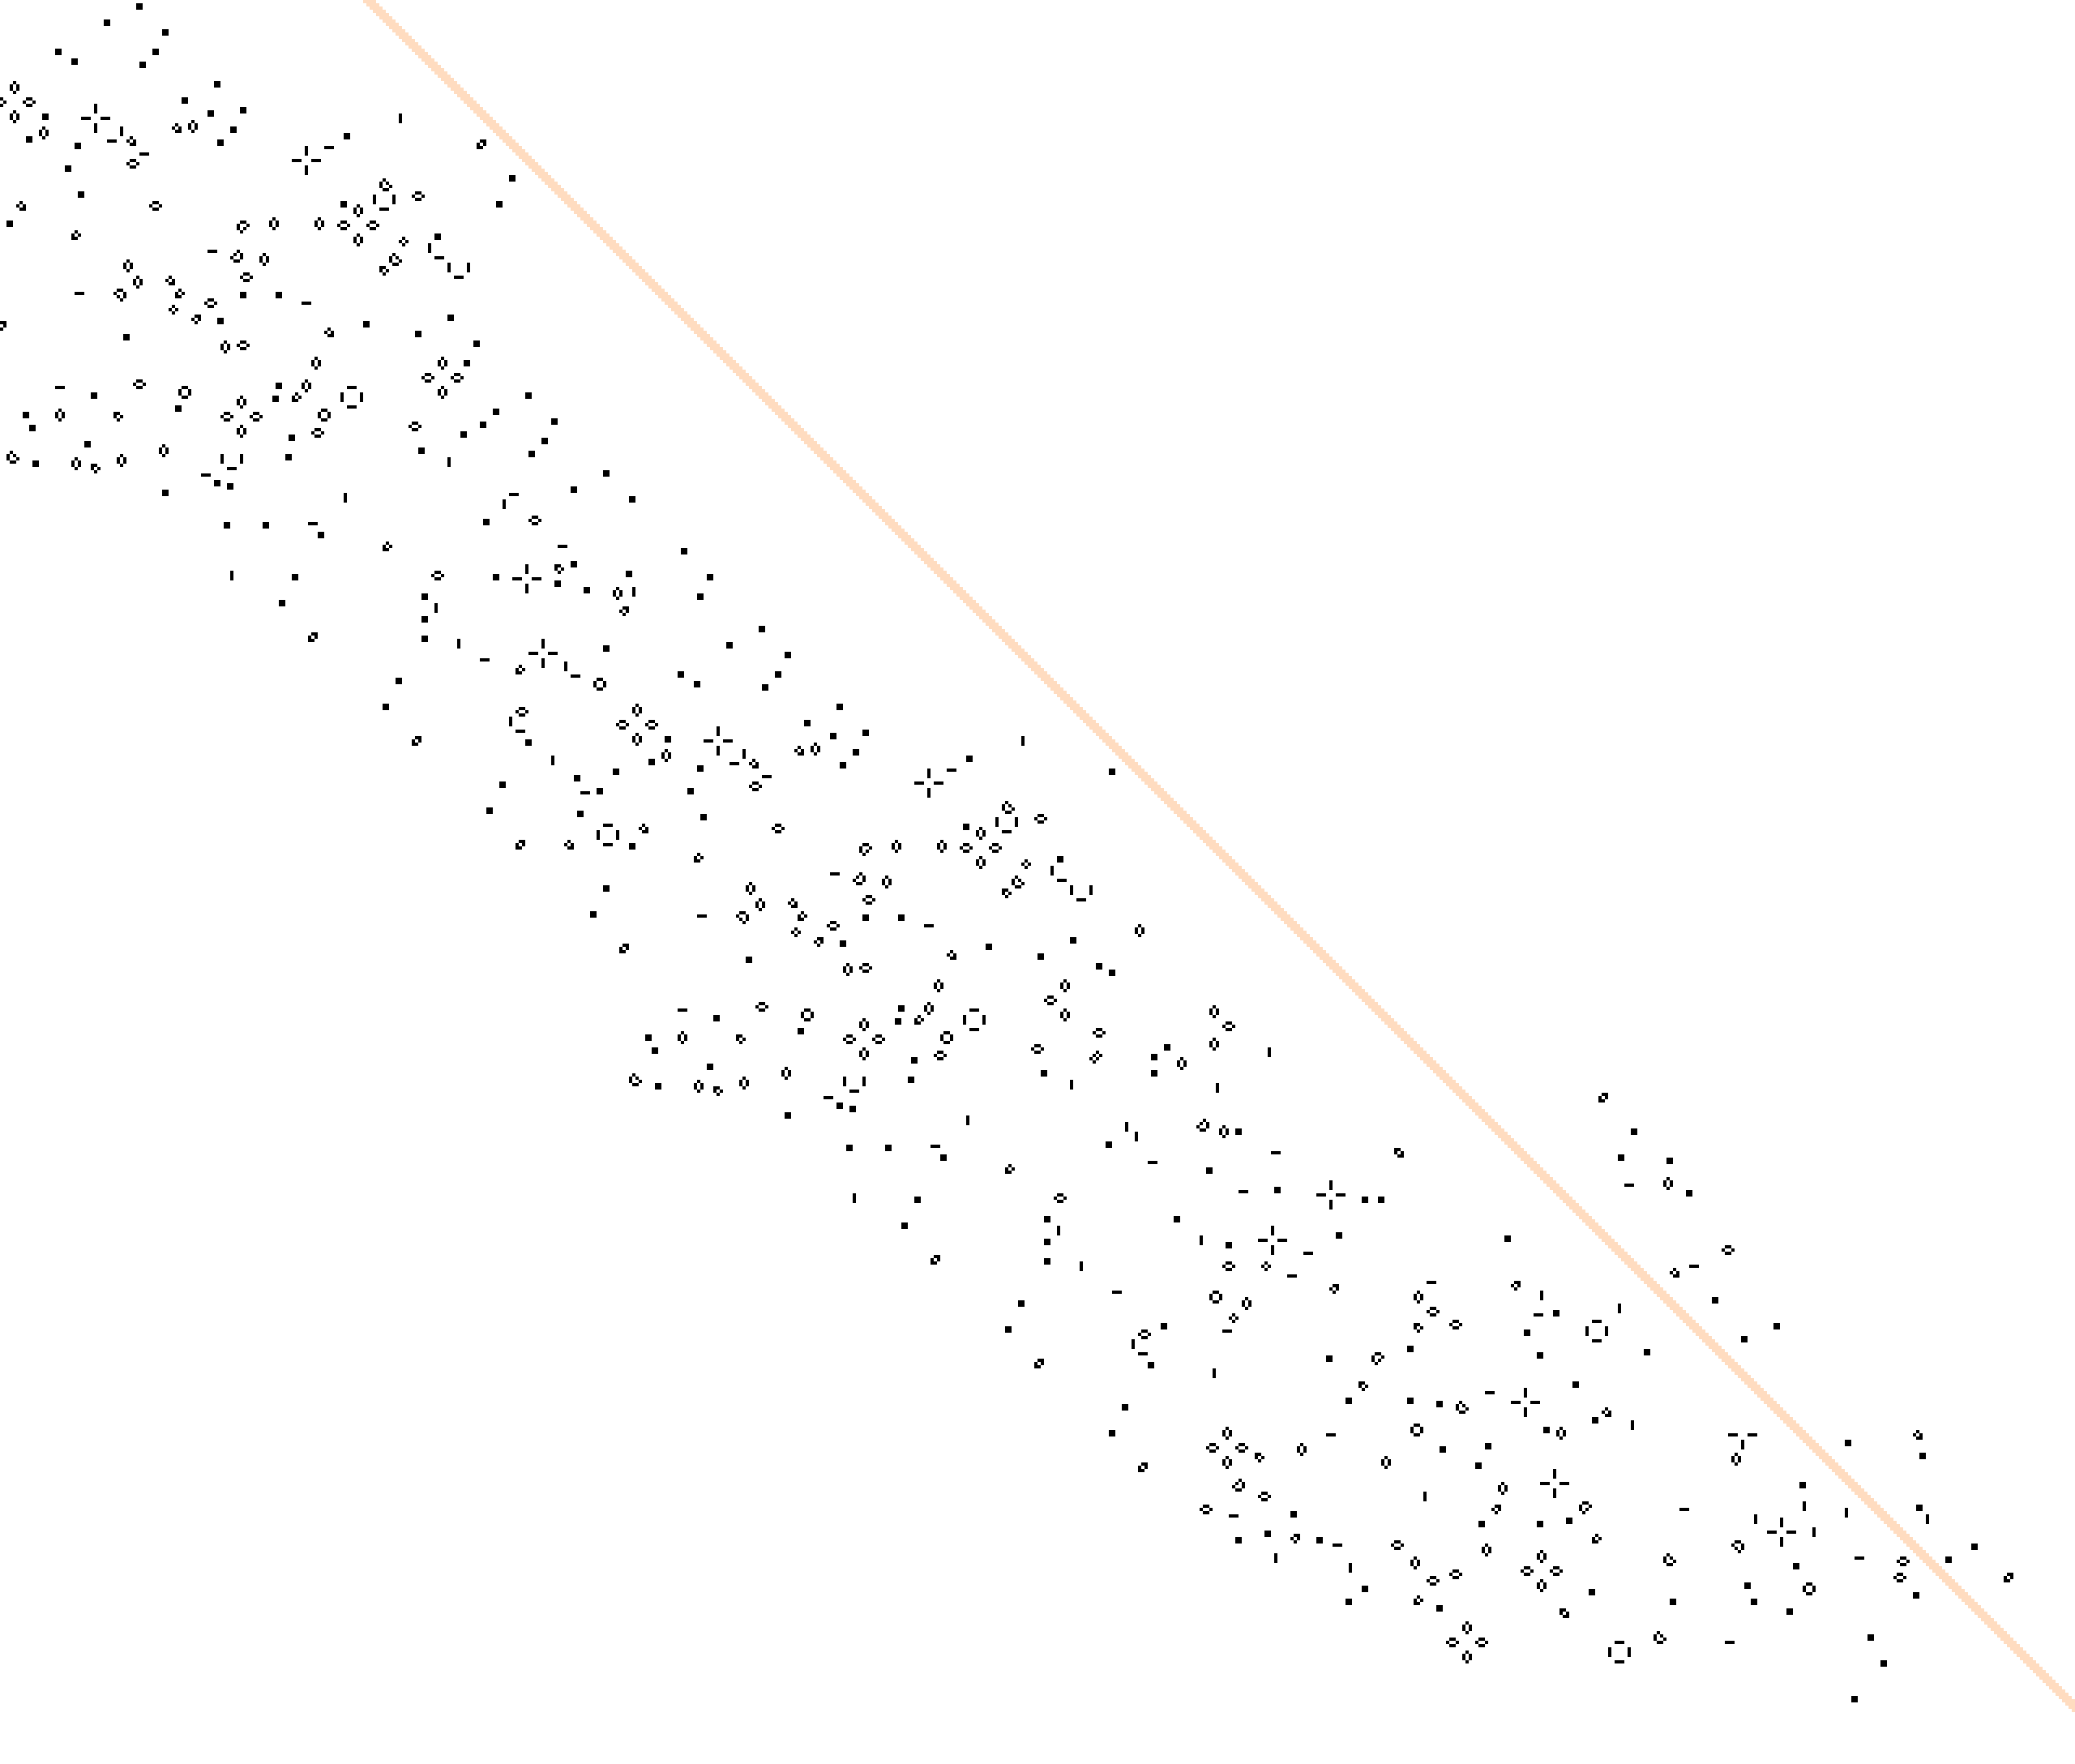
\includegraphics[width=8.53cm]{early_life/ark_736692_3.png}};
		\draw[gridgray,line width=0.75pt] (2,-9) rectangle (10.53,-1.75);
	\end{tikzpicture}
		
	\caption{The pattern from Figure~\ref{fig:ark_736692} leaves behind this absolutely massive ash after 736,692 generations. We have zoomed in by a factor of $32 \times 32 = 1,024$ on the corner of the ash that the pattern started growing from, which is also the corner that contains the debris that gliders are fired at throughout its extensive lifespan. The \bgbox{orangeback2}{orange} line on the bottom-right depicts the southeastward path taken by gliders that now (just barely) miss hitting the debris.}\label{fig:ark_736692_stabilized}
\end{figure}

While patterns like this one are certainly interesting, they are not quite in the spirit of what we want from methuselahs---even though the previous pattern did not completely stabilize for hundreds of thousands of generations, it was ``mostly'' stable for the vast majority of that time. Rather, we would like methuselahs to take a long time to stabilize based primarily on chaos that we cannot completely break down into simple reactions like gliders repeatedly hitting some debris. We will not try to make this precise, but rather just leave it as a phenomenon that we know when we see.

To briefly suggest some even more extreme examples of the weirdness that happens with stability, note that we will learn in Chapter~\ref{chp:periodic_circuitry} how to construct a pattern that computes the prime numbers. Should such a pattern be considered stable? Perhaps even more striking than this, in Section~\ref{sec:unknown_growth} we will then create a pattern whose long-term behavior we do not understand: it might continue to grow in a reasonably regular fashion indefinitely, or it might stabilize into a finite pattern. What we do know is that it continues to grow for at least its first $10^{2,500,000,000}$ generations, so if it does eventually stabilize and remain finite, it must do so after that point (and we have no hope of actually simulating the pattern long enough to find out the answer).

Even worse than this, in Chapter~\ref{chp:universal_computation} we will show that there exist patterns for which it is not \emph{possible} to know, even in principle, whether or not they stabilize. In other words, there exist patterns with the unsettling property that, no matter how long we run them, and no matter how clever we are, there is absolutely no mathematical way to know if they will eventually stabilize.


%%%%%%%%%%%%%%%%%%%%%%%%%%%%%%%%%%%%%%%%%%%%%%%%%%%%%%%%%%%%%%%%%%%%%%%%%
%%   SECTION: GARDENS OF EDEN
%%   http://wwwhomes.uni-bielefeld.de/achim/orphan.html
%%%%%%%%%%%%%%%%%%%%%%%%%%%%%%%%%%%%%%%%%%%%%%%%%%%%%%%%%%%%%%%%%%%%%%%%%
\section{Gardens of Eden}\label{sec:goe}\index{Garden of Eden}

Oftentimes, a lot can be learned by considering Life in reverse: instead of investigating what a pattern evolves into, we investigate what evolves into it. That is, we look for parents (and grandparents, and great-grandparents, ...) of the pattern that we are interested in.\footnote{Strictly speaking, if a pattern has one parent then it must have infinitely many, since we could just add any pattern that dies in one generation far away. When discussing how many parents a pattern has, we will always ignore parents that have dying ash like this that has no effect on their evolution.} Some patterns, such as the block, have numerous parents (see Figure~\ref{fig:block_parents}), which is part of the reason why they appear so frequently in the ash of random soups.

\begin{figure}[!htb]
	\centering\patternimglink{0.1}{block_parents}
	\caption{Six small parents of the block. From left-to-right, the first three of these objects are the block\index{block}, \emph{pre-block}\index{pre-block}, and \emph{grin}\index{grin}, respectively, while the other three do not have names.}\label{fig:block_parents}
\end{figure}

Other patterns, such as the clock\index{clock}, have relatively few parents and thus appear less frequently in random soups (recall that the clock has only six cells and period~2, yet appears less frequently than some much larger objects like the period~3 pulsar or the period~15 pentadecathlon). It seems natural to ask whether or not there exists a pattern that does not have even a single parent. That is, does there exist a pattern that cannot ever appear in the evolution of any other pattern, but rather can only ever appear in generation~$0$?\footnote{Generation~$0$ refers to the starting configuration, before applying the Life rules to it. Generation~$1$ is the pattern that is obtained by applying the Life rules once, and generation~$n$ is the pattern obtained by applying the Life rules $n$ times.} A pattern with this property is called a \emph{Garden of Eden},\footnote{This term was coined in the context of cellular automata by John W. Tukey in the 1950s, long before Conway's Game of Life was introduced.} and we begin by showing that they do indeed exist.

The rough idea of why Gardens of Eden must exist is that some patterns (such as blocks) have lots of parents, so there are not enough parents left over for all other patterns. To prove this explicitly, we will barely need to use anything more than the fact that blocks and pre-blocks both evolve into the same thing.\footnote{We could instead use two other objects that evolve into the same thing in the proof: we just use blocks and pre-blocks because they are so simple.}	

\begin{theorem}\label{thm:garden_of_eden_exists}
	There exist Gardens of Eden in Conway's Game of Life.
\end{theorem}

\begin{proof}
	Let $n \geq 1$ be an integer and consider all patterns that fit within a $6n \times 6n$ square on the Life grid. The contents of the central $(6n-2) \times (6n-2)$ square in generation~1 only depend on the contents of the original $6n \times 6n$ square in generation~0. This central $(6n-2) \times (6n-2)$ square contains $(6n-2)^2$ cells, each of which can be alive or dead, so there are $2^{(6n-2)^2}$ distinct patterns that could fill this central square. We will now show that, if $n$ is large enough, some of these patterns must have no parent.
	
	\begin{figure}[!htb]
		\centering\patternimg{0.1}{goe_theorem_tiles}
		\caption{Two $6 \times 6$ tiles that evolve the same way no matter what is placed outside of the tiles.}\label{fig:goe_theorem_tiles}
	\end{figure}
		
	To this end, partition the $6n \times 6n$ square into $n^2$ tiles, each of size $6 \times 6$. Each tile contains $36$ cells, each of which can be alive or dead, so there are $2^{36}$ different tiles. However, the two tiles displayed in Figure~\ref{fig:goe_theorem_tiles} evolve in the same way regardless of what other tiles are placed around them. We thus conclude that in any pattern that uses the first tile, we could replace it by the second tile without changing the evolution of the overall pattern (see Figure~\ref{fig:goe_theorem_tiles_example}). It follows that if we want to catalog all possible patterns that can be present in generation~$1$, we only need to consider patterns made up of one of $2^{36} - 1$ (not $2^{36}$) different tiles in generation~$0$.
	
	\begin{figure}[!htb]
		\centering\patternimglink{0.1}{goe_theorem_tiles_example}
		\caption{A $6n \times 6n$ pattern in the $n = 4$ case, broken down into $6 \times 6$ tiles. Each of the tiles containing only a block in the center (outlined in \bgbox{aquaback}{aqua}) can be replaced by a tile with a pre-block in the center without affecting the evolution of the overall $24 \times 24$ pattern.}\label{fig:goe_theorem_tiles_example}
	\end{figure}
	
	Since the $6n \times 6n$ square has $n^2$ of these tiles, there are at most $(2^{36}-1)^{n^2}$ different possible children (i.e., patterns present in generation~$1$). Since there are $2^{(6n-2)^2}$ distinct patterns that could fill the central $(6n-2) \times (6n-2)$ square, but at most $(2^{36}-1)^{n^2}$ of them appear in children of patterns in the $6n \times 6n$ square, all that remains is show that $(2^{36}-1)^{n^2} < 2^{(6n-2)^2}$ when $n$ is sufficiently large. Taking the $n^2$-th root of both sides of the inequality reduces it to $2^{36} - 1 < 2^{(6 - 2/n)^2}$, which is indeed true when $n$ is sufficiently large, since we can make $2/n$ arbitrarily close to $0$ and hence $2^{(6 - 2/n)^2}$ arbitrarily close to $2^{6^2} = 2^{36}$ (in particular, we can make it larger than $2^{36} - 1$).\footnote{In fact, not only is it the case that $(2^{36}-1)^{n^2} < 2^{(6n-2)^2}$ when $n$ is large, but the ratio $(2^{36}-1)^{n^2} / 2^{(6n-2)^2}$ can be made as small as we like by making $n$ sufficiently large (see Exercise~\ref{exer:goe_theorem_limit}). In other words, not only do Gardens of Eden \emph{exist}, but in fact almost all large patterns are Gardens of Edens.}
\end{proof}

It is worth noting that the method used in the proof of Theorem~\ref{thm:garden_of_eden_exists} is very general and applies to any cellular automaton for which two distinct (finite) patterns evolve into the same pattern.\footnote{This more general theorem was proved by Edward F. Moore and John Myhill in the early 1960s \cite{Moo62,Myh63}, so Gardens of Eden were known to exist in Conway's Game of Life right from the moment it was introduced.} Also, even though it is non-constructive, it can be used to find (extremely loose) bounds on how large Gardens of Eden must be---see Exercise~\ref{exer:goe_theorem}.

Now that we know that Gardens of Eden exist, our next goal is to actually find an explicit example of one.\footnote{The first explicit Garden of Eden in the Game of Life was constructed by Roger Banks in 1971.} Unfortunately, our method of proof of Theorem~\ref{thm:garden_of_eden_exists} is not of much help here, since it only shows that Gardens of Eden exist in extremely large regions (the smallest $n$ for which the inequality $(2^{36}-1)^{n^2} < 2^{(6n-2)^2}$ holds is somewhere around $n \approx 10^{12}$), and it does not actually tell us how to find one in such a region. The pattern obtained by concatenating together all $2^{n^2}$ different $n \times n$ patterns into a rectangle of size $2^{n^2} n \times n$ is guaranteed to be a Garden of Eden, but it is exponentially larger than the upper bound provided by the theorem.

Our method of construction is to build a Garden of Eden one cell at a time, repeatedly choosing the new cell that we add to the pattern so as to result in it having as few parents as possible. More explicitly, we build this Garden of Eden as follows:\footnote{This method is due to Nicolay Beluchenko \cite{A196447}.}\medskip

\begin{itemize}
	\item We consider the two possible states of a single cell. Out of the $2^9 = 512$ possible configurations of the $3 \times 3$ square centered at this cell, $372$ lead to the central cell being dead and $140$ lead to it being alive. Thus we make that central cell alive, so as to have fewer parents.\smallskip
	
	\item We then consider the two possible states of a cell that is adjacent to the starting (alive) cell. Out of the $140 \times 2^3 = 1,120$ possible configurations of the $4 \times 3$ rectangle centered at those two cells that lead to the first cell being alive, $703$ lead to the second cell being dead and $417$ lead to it being alive. We thus make the second cell alive, so as to have fewer parents.\smallskip
	
	\item We continue in this way in a clockwise spiral around the initial cell, deciding whether each new cell will be alive or dead based on which of the two possibilities results in a pattern with fewer parents.\medskip
\end{itemize}

While this method might seem not to yield anything useful at first---after 40 cells, each of them has been chosen to be alive, and the number of parents has exploded to 4,624,592---the number of parents does eventually start to dwindle, and after 266 cells the pattern has no parents at all (and is thus a Garden of Eden).\footnote{In step 262 there is a tie between the number of parents if the cell is chosen to be alive or dead. We (arbitrarily) chose the cell to be alive.} This Garden of Eden is displayed in Figure~\ref{fig:goe_1}.

\begin{figure}[!htb]
	\centering\begin{tikzpicture}%
	\node[inner sep=0pt,anchor=south west] at (0,0) {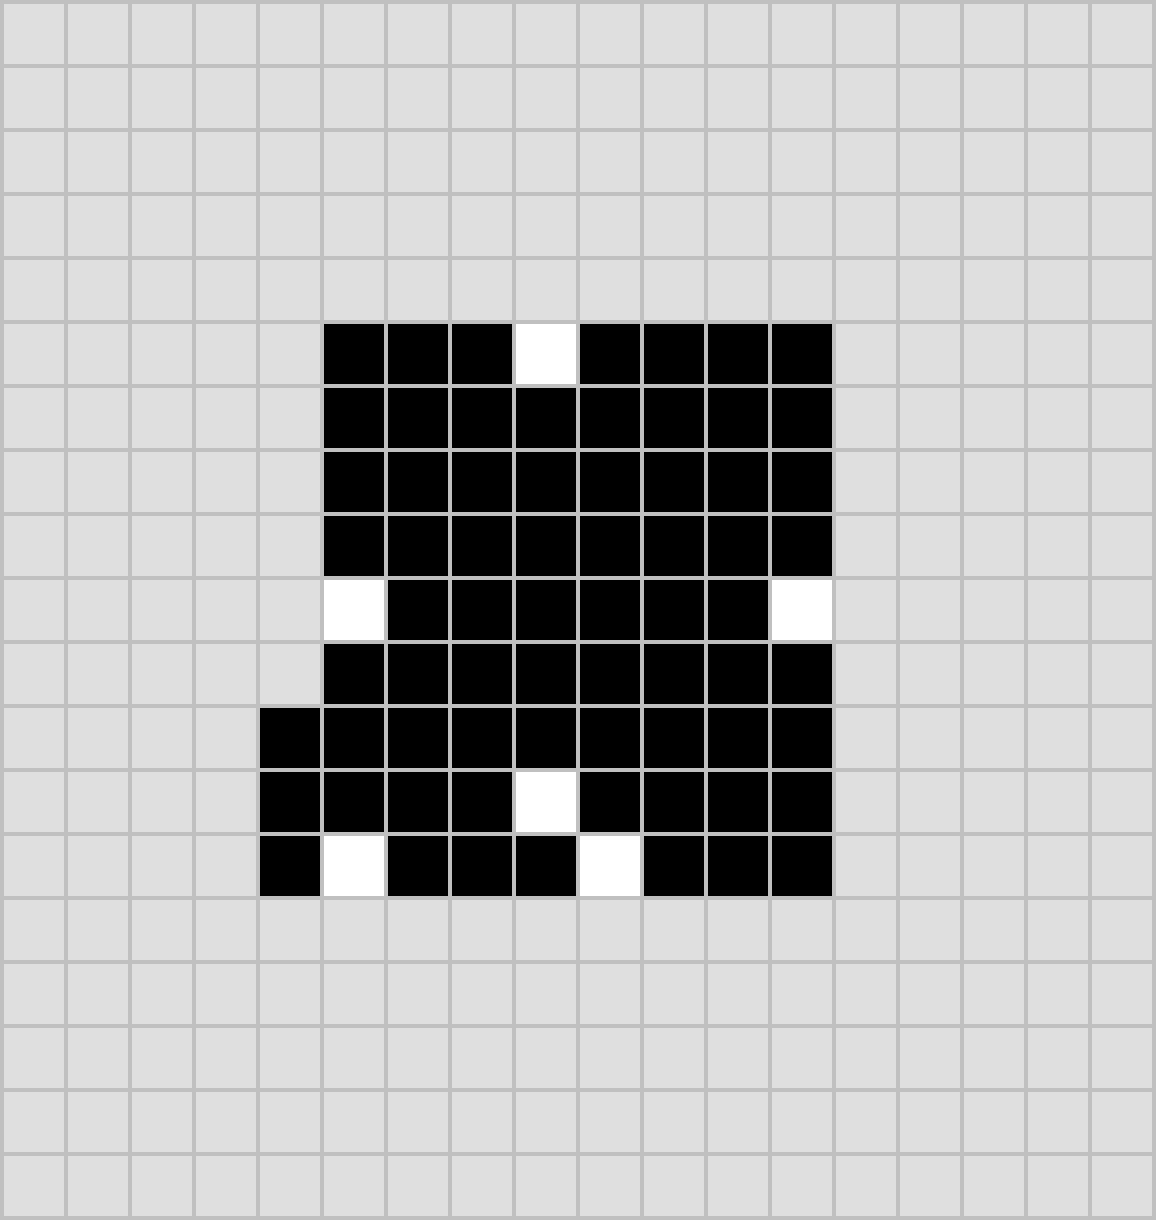
\includegraphics[width=4cm]{early_life/goe_1_partial.png}};
	\draw[->][black,line width=1pt] (1.02,1.88) -- (1.02,3.22) -- (2.4,3.22);
	
	\node[inner sep=0pt,anchor=south west] at (6,0) {\embedlink{goe_1}{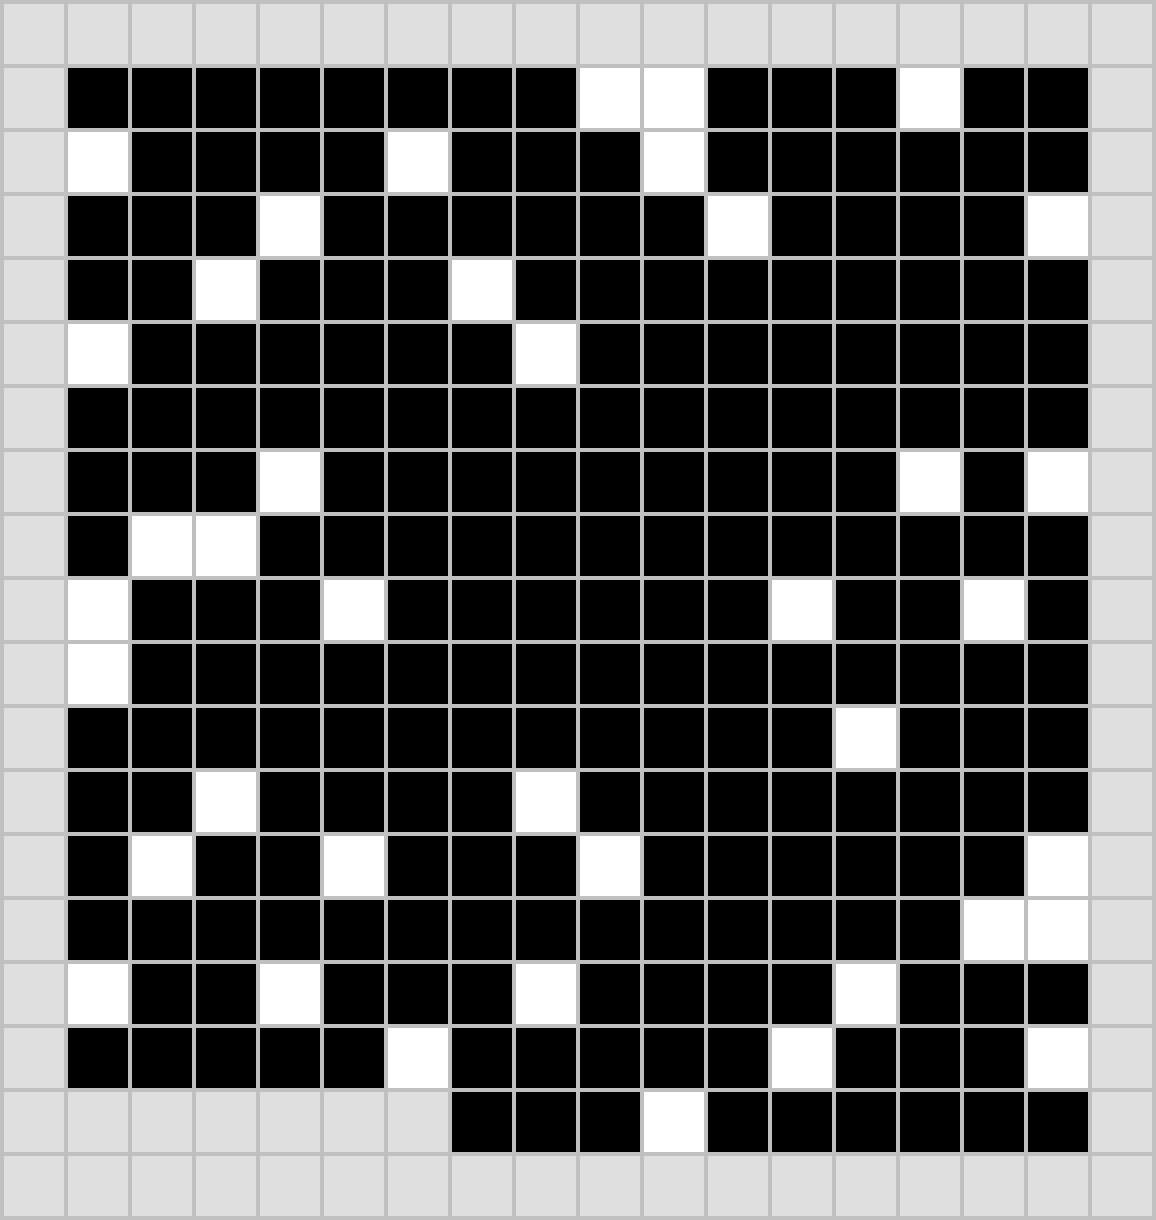
\includegraphics[width=4cm]{early_life/goe_1.png}}};
	\end{tikzpicture}
	
	\caption{A partial Garden of Eden (left) that is being constructed one cell at a time by placing cells in a clockwise spiral, choosing whether they should be alive or dead based on which state results in fewer parents. The completed Garden of Eden (right) has 41 dead cells and 225 alive cells (the \bgbox{gridgray!40}{light gray} cells are unspecified---the pattern remains a Garden of Eden regardless of whether they are alive or dead).}\label{fig:goe_1}
\end{figure}

The pattern that we have constructed is interesting in that it is not only a Garden of Eden, but it remains a Garden of Eden regardless of what live and dead cells we place outside of the central 266-cell spiral. Patterns like this one that cannot be \emph{any} part of the evolution of another pattern (equivalently, they are still a Garden of Eden no matter what other cells are placed around them) are called \emph{orphans}\index{orphan}.\footnote{This term was coined by Conway. Also, the proof of Theorem~\ref{thm:garden_of_eden_exists} actually demonstrates the existence of orphans, not just Gardens of Eden.} Every pattern containing an orphan is (by definition) a Garden of Eden, but it is currently unknown whether or not there exists a Garden of Eden that does not contain an orphan.
	
Now that we know that small Gardens of Eden (and orphans) exist, we would like to know how small and simple they can be. A complete answer to this problem is still open (and perhaps is currently one of the most actively-researched problems in Life), but many partial results are known. The smallest known orphans and Gardens of Eden (in terms of number of cells and bounding box size) are presented in Figure~\ref{fig:goe_records}.\footnote{These patterns can be verified to be orphans via a computer program called \emph{JavaLifeSearch}---see \httpsurl{conwaylife.com/wiki/JavaLifeSearch} and Exercise~\ref{exer:goe_jls}.}\index{JavaLifeSearch}

\begin{figure}[!htb]
	\centering
	\begin{subfigure}{.31\textwidth}
		\centering
		\patternimglink{0.1}{goe_record_alive}
		\caption{A Garden of Eden with 45~live cells, found by Nicolay Beluchenko in 2009.}
		\label{fig:goe_record_alive}
	\end{subfigure} \ \ \ \ % 
	\begin{subfigure}{.31\textwidth}
		\centering
		\patternimglink{0.1}{goe_record_orphan}
		\caption{An orphan with 88~specified cells, found by Steven Eker in 2017.} % No longer cited? \cite{HHKN11}
		\label{fig:goe_record_orphan}
	\end{subfigure} \ \ \ \ % 
	\begin{subfigure}{.31\textwidth}
		\centering
		\patternimglink{0.1}{goe_record_bb}
		\caption{A Garden of Eden in a bounding box with area $96 = 8 \times 12$, found by Steven Eker in 2016.}
		\label{fig:goe_record_bb}
	\end{subfigure}
	\caption{The current smallest-known Gardens of Eden by (a)~number of live cells, (b)~total number of live and dead cells specified in the orphan, and (c)~bounding box area.}\label{fig:goe_records}
\end{figure}

On the other hand, there are also results that show that orphans cannot be ``too'' small. For example, exhaustive computer searches have shown that there does not exist an orphan that fits within a $6 \times 7$ bounding box.\footnote{This computation was carried out independently by Steven Eker and Marijn Heule in 2016.} In a similar vein, we now show that there does not exist a Garden of Eden that has a bounding box with height one.\footnote{This theorem was originally proved by Jean Hardouin--Duparc in 1974 \cite{Har74}.}

\begin{theorem}\label{thm:1_row_goe}
	In Conway's Game of Life, every pattern that fits within a bounding box of height~$1$ has a parent. In other words, there do not exist Gardens of Eden with height~$1$.
\end{theorem}

\begin{proof}
	We prove the theorem by explicit construction: we show how to find a parent of any $1$-cell-thick pattern. The key step in our construction is to build a border that dies off completely in one generation and guarantees that any junk placed inside of it does not expand outward in that generation. Figure~\ref{fig:1_row_border} shows one such border: no matter what we place inside the $3 \times n$ box in the middle of the border, no cell outside of that $3 \times n$ box will be alive in the next generation.
	
	\begin{figure}[!htb]
		\centering\patternimglink{0.12}{1_row_border}
		\caption{A border that can be used to help construct parents of 1-cell-thick patterns. No matter what we place in the central $3 \times n$ region, no cell outside of the $3 \times n$ region will be alive in the next generation. We will fill it in such a way so that the desired $1 \times (n-2)$ pattern evolves in the center row, highlighted in \bgbox{aquaback}{aqua}).}\label{fig:1_row_border}
	\end{figure}
	
	To complete the proof, we just need to find a way to fill that $3 \times n$ box in such a way that it evolves into any $1 \times (n-2)$ pattern that we desire. One simple method that \emph{almost} works is to put the desired pattern itself in the central row of the $3 \times n$ box, and its negation (i.e., flip all alive cells to dead and vice-versa) in the top and bottom rows of the $3 \times n$ box. It is straightforward to check that the cells in the top and bottom rows of the $3 \times n$ box will always be overpopulated, and thus those two rows will always be dead in the next generation. Furthermore, the central row evolves in the correct way in 7 out of every 8 possible configurations of three adjacent alive/dead cells (see Figure~\ref{fig:1_row_3x3}).

	\begin{figure}[!htb]
		\centering
		\begin{minipage}[b]{0.64\textwidth}
			\centering\begin{tikzpicture}[scale=1.1, every node/.style={transform shape}]%
				\fill[color=redback] (2.2,0.95) rectangle (3.25,-1.35);
				\node[inner sep=0pt,anchor=south west] at (0,0) {\patternimg{0.102}{1_row_3x3}};
				\node[inner sep=0pt,anchor=south west] at (0.3,-0.52) {$\downarrow \qquad \ \ \downarrow \qquad \ \ \downarrow \qquad \ \ \downarrow \qquad \ \ \downarrow \qquad \ \ \downarrow \qquad \ \ \downarrow \qquad \ \ \downarrow$};
				\node[inner sep=0pt,anchor=south west] at (0.23,-1.1) {\patternimg{0.102}{1_row_3x3_evolved}};
			\end{tikzpicture}
			\caption{All except for one of the $8$~different $3 \times 3$ squares in which the top and bottom rows are the negation of the middle row evolve so that the top and bottom rows die and the middle cell stays the same.}\label{fig:1_row_3x3}
		\end{minipage}\hfill\begin{minipage}[b]{0.32\textwidth}
			\centering\gridbox{1pt}{\begin{tikzpicture}[scale=0.5, every node/.style={transform shape}]%
				\node[inner sep=0pt,anchor=south west] (glider_loop) at (0.5,0.5) {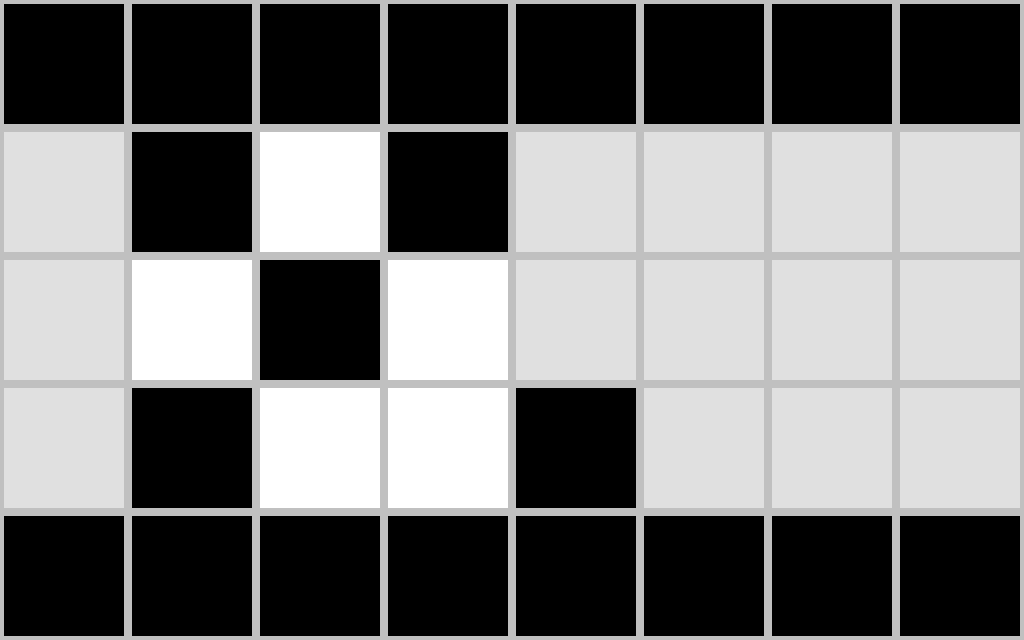
\includegraphics[width=6cm]{early_life/goe_1_row_proof.png}};
				%\draw[black!20,line width=2pt] (0,0) rectangle (5,-5);
				
				\letternode{4}{2}{A}
				
				\letternode{5}{3}{X}
				\letternode{5}{2}{Y}
				\end{tikzpicture}}
			\caption{In order to correct the problematic $3 \times 3$ block from Figure~\ref{fig:1_row_3x3}, we set cell~A to be dead and cell~Y to be alive, regardless of the state of cell~X.}\label{fig:goe_row_1_proof}
		\end{minipage}
	\end{figure}
	
	To fix the problem that occurs when a single alive cell is between two dead cells in the middle row, simply set the bottom-right cell (i.e., cell~A in Figure~\ref{fig:goe_row_1_proof}) of that $3 \times 3$ block as dead, rather than alive. To compensate for this cell being dead, we also set the cell to its immediate right (i.e., cell~Y in that figure) to be alive, regardless of whether cell~X is alive or dead. It is then straightforward to verify that the resulting pattern will evolve into the $1 \times (n-2)$ pattern that we desire: all that needs to be checked is that the central cell in this $3 \times 3$ block now stays alive (since it now has exactly 3 live neighbors) and that moving the alive cell from A to Y does not affect the evolution of any of the other $3 \times 3$ blocks to its right (which can be done via a simple case analysis).
\end{proof}

The method used in the proof of Theorem~\ref{thm:1_row_goe} is illustrated in Figure~\ref{fig:goe_1_row_eg}, where we start with a (randomly-chosen) pattern with height~$1$ and explicitly construct a parent of it.
\begin{figure}[!ht]
	\centering\begin{tikzpicture}[scale=1.25, every node/.style={transform shape}]%
		\node[inner sep=0pt,anchor=west] at (0,0) {\embedlink{1_row_eg}{\patternimg{0.1}{1_row_eg_1}}};
		\draw [->,rounded corners=0.25cm] (7.75,-0.4) -- (8.25,-0.4) -- (8.25,-0.9);
		\node[inner sep=0pt,anchor=west] at (2.3,-2.1) {\patternlink{1_row_eg}{\patternimg{0.1}{1_row_eg_2}}};
		\draw [->,rounded corners=0.25cm] (10.05,-2.5) -- (10.55,-2.5) -- (10.55,-3.0);
		\node[inner sep=0pt,anchor=west] at (4.6,-4.2) {\patternlink{1_row_eg}{\patternimg{0.1}{1_row_eg_3}}};
	\end{tikzpicture}
	\caption{How to use the proof of Theorem~\ref{thm:1_row_goe} to construct a parent (at the bottom) of a pattern with height~$1$ (at the top). First, we place the border around the pattern (displayed in \bgbox{redback2!25!redback}{dark red} in the middle image) and place the pattern's negation in the top and bottom rows of the box (displayed in \bgbox{greenback}{dark green} in the middle image). We then adjust the bottom row slightly (highlighted in \bgbox{greenpastel}{light green} in the bottom image) whenever we see the troublesome configuration from Figure~\ref{fig:goe_row_1_proof}.}\label{fig:goe_1_row_eg}
\end{figure}

More sophisticated techniques have been used to prove that there similarly do not exist orphans whose bounding boxes are $2$ or $3$ cells high.\footnote{This was proved by Steven Eker in 2016, using the same computer-assisted methods introduced by Jean Hardouin--Duparc.} On the other hand, there does exist an orphan (and thus a Garden of Eden) with height~$5$, as shown in Figure~\ref{fig:goe_height_5}.\footnote{This orphan was also found by Steven Eker in 2016.} The question of whether or not there exists an orphan whose bounding box is $4$ cells high remains open.

\begin{figure}[!htb]
	\centering\embedlink{goe_height_5}{\patternimg{0.1}{goe_height_5}}
	\caption{A Garden of Eden and orphan that fits within a $5 \times 45$ bounding box. No Garden of Eden with height less than $5$ is currently known.}\label{fig:goe_height_5}
\end{figure}


%%%%%%%%%%%%%%%%%%%%%%%%%%%%%%%%%%%%%%%%%%%%%%%%%%%%%%%%%%%%%%%%%%%%%%%%%
%%   SUBSECTION: A PATTERN WITH NO GRANDPARENT
%%%%%%%%%%%%%%%%%%%%%%%%%%%%%%%%%%%%%%%%%%%%%%%%%%%%%%%%%%%%%%%%%%%%%%%%%
\subsection{A Pattern with no Grandparent}\label{sec:no_grandparent}

There are many very difficult follow-up questions that can be asked about Gardens of Eden or patterns with properties related to those of Gardens of Eden. For example, does there exist a pattern that has a parent but no grandparent? In other words, does there exist a pattern with the property that all of its parents are Gardens of Eden? Although there is no known non-constructive argument like the one used in the proof of Theorem~\ref{thm:garden_of_eden_exists} that shows the existence of such patterns, it turns out that the answer to this question is ``yes'', and an example of such a pattern is presented in Figure~\ref{fig:grandparentless}. This pattern has the remarkable property that it has 17,920 distinct parents, every single one of which is a Garden of Eden---one of these parents is displayed in Figure~\ref{fig:grandparentless_parent}.\footnote{Whether or not such a pattern exists was originally asked by Conway in October 1972. It was not resolved until May 2016, when the pattern displayed in Figure~\ref{fig:grandparentless} was found by user ``mtve'' on the ConwayLife.com forums. Later that month, they even found a pattern that has a grandparent but no great-grandparent and a pattern with a great-grandparent but no great-great-grandparent, though the question remains open of whether or not, for every integer $n \geq 1$, there exists a pattern with a great$^n$-grandparent but no great$^{n+1}$-grandparent.}

\begin{figure}[!htb]
	\centering
	\begin{minipage}[b]{.48\textwidth}
		\centering\vspace*{0.11cm}
		\patternimglink{0.12}{grandparentless}
		\caption{A pattern that has a parent but no grandparent.}\label{fig:grandparentless}
	\end{minipage} \quad %
	\begin{minipage}[b]{.48\textwidth}
		\centering
		\patternimglink{0.092}{grandparentless_parent}
		\caption{A parent of the grandparentless pattern from Figure~\ref{fig:grandparentless}.}\label{fig:grandparentless_parent}
	\end{minipage}
\end{figure}

The method used to construct this pattern is almost identical to the method we used to construct the Garden of Eden in Figure~\ref{fig:goe_1}. That is, it was constructed one cell at a time, and each new cell that was added was chosen to be either alive or dead based on which of the two options resulted in the pattern having fewer grandparents.


%%%%%%%%%%%%%%%%%%%%%%%%%%%%%%%%
\section*{Notes and Historical Remarks}
\label{sec:early_life_notes}
\addcontentsline{toc}{section}{\nameref{sec:early_life_notes}}
%%%%%%%%%%%%%%%%%%%%%%%%%%%%%%%%

Conway's Game of Life was initially studied by John Conway and some of his collaborators at Cambridge University, as well as a research group led by Bill Gosper at MIT, in 1969 and 1970. It then received mainstream attention in 1970 due to an article that Martin Gardner wrote about it in the magazine \emph{Scientific American}\index{Scientific American} \cite{Gar70} (see Figure~\ref{fig:sci_am_1970}). Early discoveries by enthusiasts were sent to Gardner, who then shared those discoveries with Conway and, due to the overwhelming response to his article, wrote a follow-up article in February 1971 \cite{Gar71}.

It was unsustainable for Martin Gardner to continue to serve as curator for all Life discoveries, and Scientific American would only agree to so many articles on the subject, so in March 1971 a quarterly newsletter called \emph{Lifeline}\index{Lifeline} was announced, which was edited and distributed by Robert Wainwright (see Figure~\ref{fig:lifeline}). This newsletter had 11 editions, and included the announcement of many of the objects that we saw in this chapter, including the twin bees gun, the switch engine (and its block-laying and glider-producing variants), and the acorn methuselah. Its final issue was dated September 1973.

\begin{figure}[!htb]
	\centering
	\begin{minipage}[b]{0.48\textwidth}
		\centering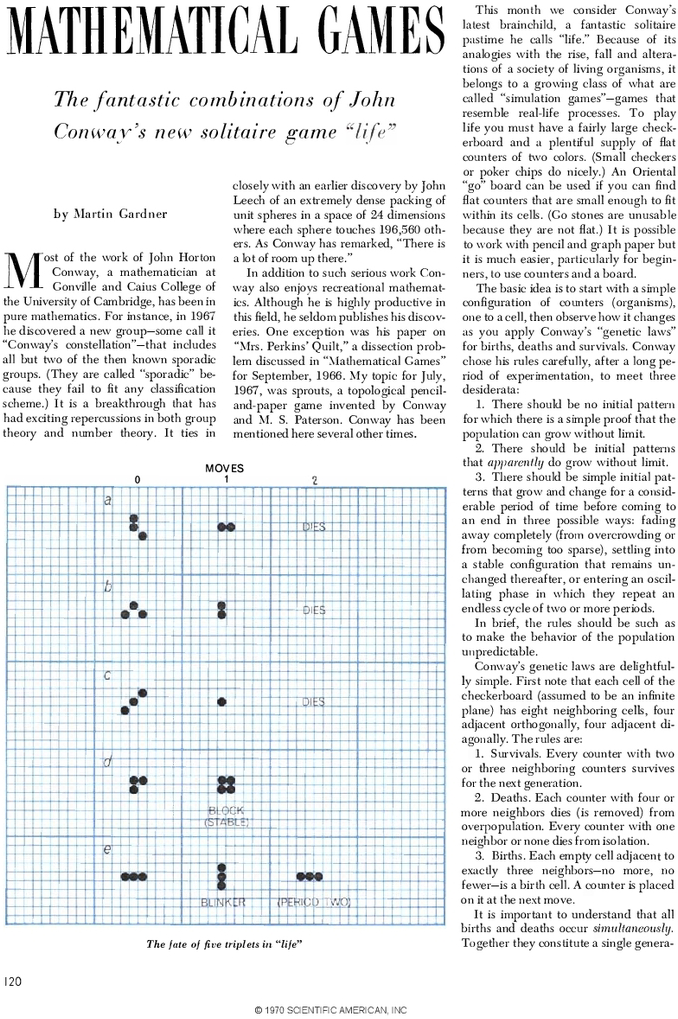
\includegraphics[width=0.75\textwidth]{early_life/sci_am_1970.png}
		\caption{Conway's Game of Life was popularized by the October 1970 issue of \emph{Scientific American}.}\label{fig:sci_am_1970}
	\end{minipage}\hfill
	\begin{minipage}[b]{0.48\textwidth}
		\centering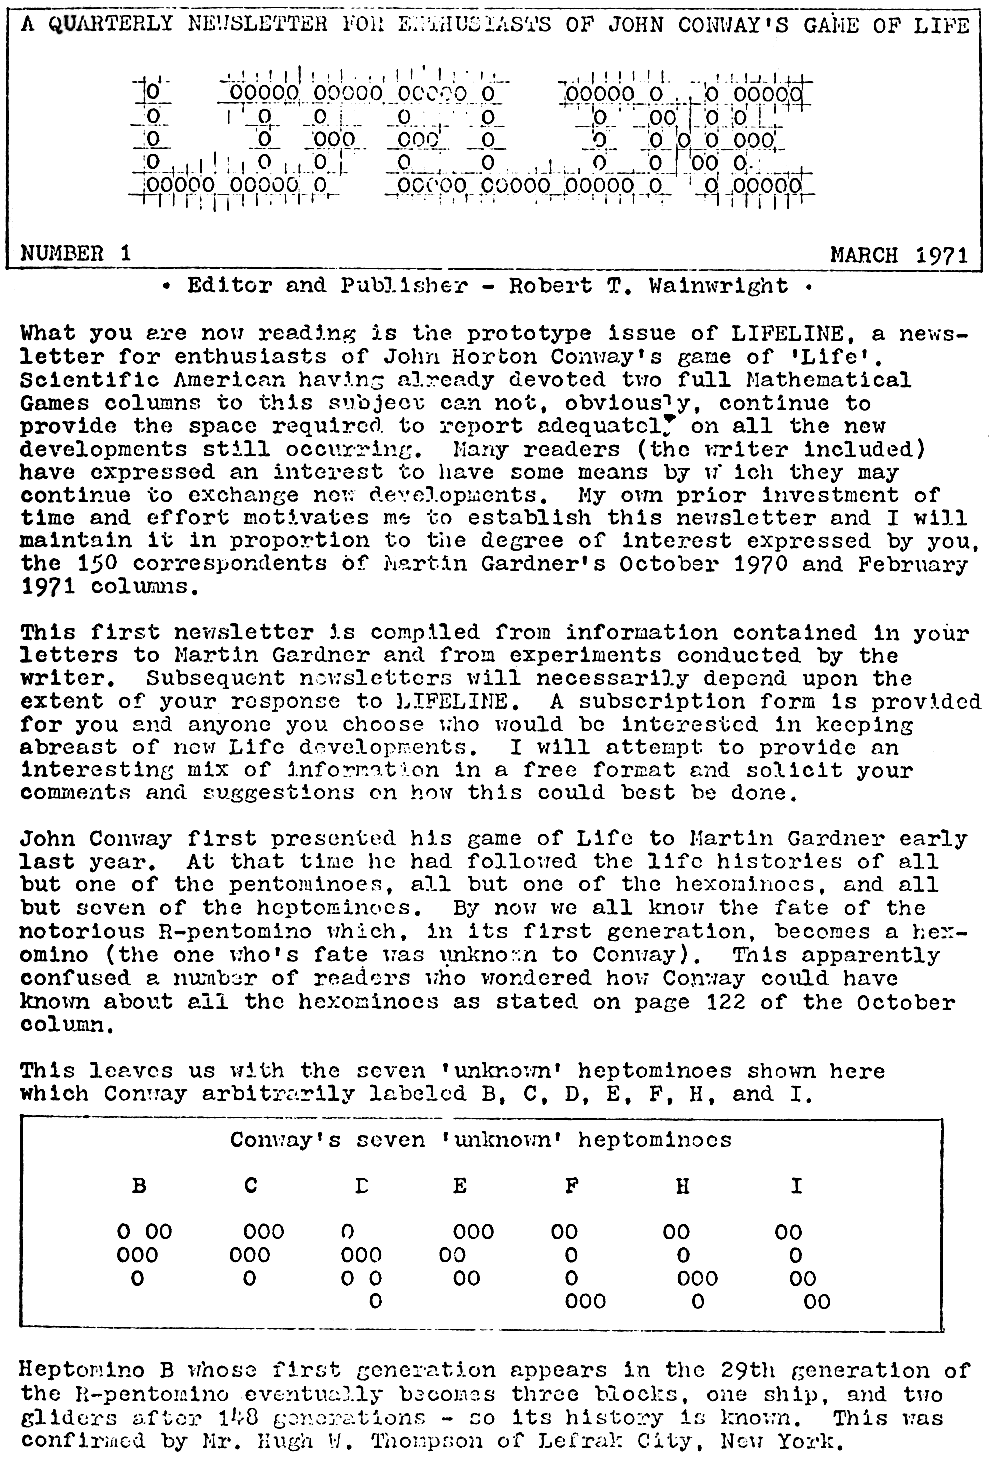
\includegraphics[width=0.75\textwidth]{early_life/lifeline_vol1.png}
		\caption{The front page of the first issue of \emph{Lifeline}, a newsletter for Life enthusiasts that ran from March 1971 to September 1973.}\label{fig:lifeline}
	\end{minipage}
\end{figure}

From 1974 to 2009, Life enthusiasts mostly shared patterns via various private mailing lists, and collections of those patterns made their way to various personal web pages in the 1990s. In 2004, the LifeNews website was launched at \httpurl{pentadecathlon.com}, which posted most interesting new Life discoveries as they were made. Since about 2009, most new discoveries in Life are now reported on the forums at \httpsurl{conwaylife.com}.

Although more advanced techniques are now known for constructing interesting Life objects (indeed, these techniques comprise the majority of the rest of this book), the idea of simply running randomly-generated soups to completion to see what remains of them after they stabilize has been a consistent one. However, because computing power was at much more of a premium in 1970 than it is now, and there was no pre-made Life simulation software for early enthusiasts to use, these patterns were often evolved by hand using graph paper, checkers, or the board and stones from the game Go, to represent the Life grid and its live cells.

Furthermore, the methodology that was used back then was somewhat more systematic---instead of generating large random starting configurations, early Lifers investigated the evolution of all possible small starting configurations. These investigations were exactly where the original interest in the T-tetromino,\index{T-tetromino} R-pentomino,\index{R-pentomino} B-heptomino,\index{B-heptomino} stairstep hexomino\index{stairstep hexomino}, and other small polyominoes came from. In fact, the switch engine was originally found by Charles Corderman when he was investigating the evolution of nonominoes (i.e., polyominoes with $9$ live cells), one of which evolves in the exact same way as the switch engine (see Figure~\ref{fig:switch_engine_nonomino}).

Solomon W. Golomb invented the term "polyomino" in 1953, and Martin Gardner wrote a popular Mathematical Games article about them a decade before the first article on Conway's Game of Life. Perhaps partly because of this long-standing interest in polyominoes in the mathematical community, the fates of N-cell polyominoes were exhaustively researched very early on, giving rise to the common names of many of the active patterns discussed above.  The Moore-neighborhood equivalent of polyominoes, the N-cell \emph{polyplets}\index{polyplet}---cell groups that are kingwise-connected rather than rookwise-connected--- are technically just as relevant as a potential source of novelty, but their evolutionary fates were much less thoroughly explored in the early years than the polyominoes.

\begin{figure}[!htb]
	\centering
	\begin{subfigure}{.48\textwidth}
		\centering \embedlink{nonomino}{\vcenteredhbox{\patternimg{0.1}{switch_engine_nonomino_0}} \vcenteredhbox{\genarrow{2}} \vcenteredhbox{\patternimg{0.1}{switch_engine_nonomino_2}}}
		\caption{A nonomino.}\label{fig:switch_engine_nonomino_non}
	\end{subfigure} \ \ \ \ % 
	\begin{subfigure}{.48\textwidth}
		\centering \patternlink{switch_engine}{\vcenteredhbox{\patternimg{0.1}{switch_engine_not_nonomino_0}} \vcenteredhbox{\genarrow{2}} \vcenteredhbox{\patternimg{0.1}{switch_engine_not_nonomino_2}}}
		\caption{A switch engine.}\label{fig:switch_engine_nonomino_not}
	\end{subfigure}
	\caption{The nonomino~(a) evolves in the same way as the switch engine~(b) after $2$ generations.}\label{fig:switch_engine_nonomino}
\end{figure}

Building upon this idea of finding objects by evolving random starting configurations, Achim Flammenkamp ran an automated computer search in 1994 that repeatedly generated random soups and evolved them, keeping a list of all objects that it found in the resulting ash. This search ran until it had accumulated $5 \times 10^9$ (non-distinct) ash objects, which contained a total of $48$ distinct oscillators \cite{Fla94}. He then performed this search again in 2004, this time accumulating $5 \times 10^{10}$ ash objects, and found over 3,500 distinct still lifes and over 80 different oscillators \cite{Fla04}.

Andrzej Okrasinski created a similar program that acted as a screensaver in November~2003. Over the subsequent 5~years, this screensaver catalogued over $4.7 \times 10^{11}$ ash objects, including over 8,000 distinct still lifes and about 180 oscillators, but still the only spaceships that turned up were the four that we have already seen (the glider, LWSS, MWSS, and HWSS) \cite{Okr03}. The screensaver also kept track of how long each starting configuration took to stabilize, and found some new methuselahs in the process, including a 15-cell version of Lidka, which was presented in Table~\ref{tab:small_methuselahs} (it was improved to a 13-cell version by David Bell and then to the more compact 13-cell version presented in that table by Simon Ekström).

In 2009, Nathaniel Johnston created a distributed online search to continue in this vein, called \emph{The Online Life-Like CA Soup Search} (or \emph{TOLLCASS}\index{TOLLCASS} for short). This script had the advantage that multiple people could run it simultaneously on different computers, and their results were automatically uploaded to a central server that organized them. TOLLCASS also worked not just with Conway's Game of Life, but also with a handful of other Life-like cellular automata. The major downside of this script was that it was quite slow, and over the two years that it was active, it catalogued only about one third as many objects as Okrasinski's earlier search.

Finally, Adam P. Goucher launched another distributed online search in 2014 called \emph{apgsearch}\index{apgsearch},\footnote{Officially, the ``apg'' in apgsearch are not its author's initials, but rather stand for \textbf{a}sh \textbf{p}attern \textbf{g}enerator.} which is still active today\footnote{It is available at \httpsurl{catagolue.appspot.com}.} and is the current state-of-the-art when it comes to soup searching. Like TOLLCASS, it can be used with several different Life-like CA, but with the main advantage of being extremely fast. In the six years since it began, it has catalogued more than 1,000 times as many ash objects as all of the previous searches combined (and this number will likely become out of date very quickly). A summary of these various soup searches that have taken place over the years is provided by Table~\ref{tab:ash_searches}.

\begin{table}[!htb]\vspace*{0.05in}
	\begin{center}		
		\begin{tabular}{l c c l}
			\toprule
			Search Name & Year(s) & Ash Objects Found & Notes \\ \midrule
			Flammenkamp & 1994 & $5.0 \times 10^9$ & first automated soup search \\
			\rowcolor{gray!20} Flammenkamp & 2004 & $5.0 \times 10^{10}$ & -- \\
			Okrasinski & 2003--2008 & $4.7 \times 10^{11}$ & also found methuselahs \\
			\rowcolor{gray!20} TOLLCASS & 2009--2011 & $1.7 \times 10^{11}$ & online search, multiple CA \\
			apgsearch & 2014--present & $7.2 \times 10^{14}$ & online search, multiple CA \\
			\bottomrule
		\end{tabular}
		\caption{A summary of the different soup searches that have taken place over the years.}\label{tab:ash_searches}
	\end{center}
\end{table}


\filbreak


%%%%%%%%%%%%%%%%%%%%%%%%%%%%%%%%%
\section*{Exercises \hfill \normalfont\textsf{\small solutions to starred exercises on \hyperlink{solutions_early_life}{page \pageref{solutions_early_life}}}}
\label{sec:early_life_exercises}
\addcontentsline{toc}{section}{Exercises}
\vspace*{-0.4cm}\hrulefill\vspace*{-0.3cm}\footnotesize\begin{multicols}{2}\vspace*{-0.4cm}\raggedcolumns\interlinepenalty=10000
\setlength{\parskip}{0pt}
%%%%%%%%%%%%%%%%%%%%%%%%%%%%%%%%%

\begin{problemstar}\label{exer:natural_switch_engine}
	Evolve each of the following randomly-generated $20 \times 20$ soups and describe the most unusual object that forms.\vspace*{-0.25cm}
	
	\begin{multicols}{2}
		\begin{enumerate}
			\item[\bf\color{ocre}(a)] \raisebox{-\height+\ht\strutbox}{\patternimglink{0.1}{exercise_random_3}}
			
			\item[\bf\color{ocre}(c)] \raisebox{-\height+\ht\strutbox}{\patternimglink{0.1}{exercise_random_4}}
			
			\item[\bf\color{ocre}(b)] \raisebox{-\height+\ht\strutbox}{\patternimglink{0.1}{exercise_random_1}}
			
			\item[\bf\color{ocre}(d)] \raisebox{-\height+\ht\strutbox}{\patternimglink{0.1}{exercise_random_2}}
		\end{enumerate}
	\end{multicols}
\end{problemstar}


\mfilbreak


\begin{problem}\label{exer:4_cell_methuselahs}
What is the longest lifespan of a pattern with:\smallskip

\begin{enumerate}[label=\bf\color{ocre}(\alph*)]
	\item $1$ or $2$ live cells?
	% SOLUTION: 1
	
	\item $3$ live cells?
	
	\item $4$ live cells? [Hint: You could try writing a computer program to help you.]
\end{enumerate}
\end{problem}


\mfilbreak


\begin{problem}\label{exer:pentominoes}
All 12 different pentominoes are displayed below. What are their lifespans?

\begin{center}
	\patternimglink{0.1}{exercise_pentominoes}
\end{center}
\end{problem}


\mfilbreak


\begin{problem}\label{exer:twin_bees_stabilize}
In this exercise, we will find some alternate stabilizations of the twin bees shuttle from Figure~\ref{fig:twin_bees_shuttle}.\smallskip

\begin{enumerate}[label=\bf\color{ocre}(\alph*)]
	\item Try removing some of the blocks from the twin bees shuttle. Which combinations of blocks can you remove while preserving it as a period~46 oscillator?
	% Can remove up to one block from each side
	
	\item The still life below is called a \emph{hat}\index{hat}. Use a hat to stabilize one side of the twin bees shuttle.
	\begin{center}
		\patternimglink{0.1}{hat}
	\end{center}
	% SOLUTION:
	% x = 29, y = 11, rule = B3/S23
	% 17bo$2o15b2o$2o16b2o$13b2o2b2o6bo$25b3o$28bo$25b3o$13b2o2b2o6bo$2o16b2o$2o15b2o$17bo!
\end{enumerate}
\end{problem}


\mfilbreak


\begin{problemstar}\label{exer:find_unstable}
Find a specific generation at which each of the following unstable objects appears in the evolution of the R-pentomino.\smallskip

\begin{enumerate}[label=\bf\color{ocre}(\alph*)]
	\item A T-tetromino.
	
	\item A pre-honey farm.
	
	\item A pi-heptomino.
	
	\item A queen bee.
	
	\item Lumps of muck (in particular, generation~$3$ of the stairstep hexomino).
\end{enumerate}
\end{problemstar}


\mfilbreak


\begin{problem}\label{exer:double_gosper_gun}
Use two blocks and three queen bees to create a ``double'' Gosper glider gun: a gun that emits two streams of gliders.
\end{problem}
% SOLUTION:
% x = 50, y = 13, rule = B3/S23
%36b2o$38bo$25b2o12bo8b2o$25b2o4bo7bo8b2o$11bo10b2o5b2o8bo$11bobo7b3o5b
%o2b2o4bo$2o12b2o6b2o6b5ob2o$2o12b2o9b2o4bo$14b2o9b2o$11bobo$11bo11bo
%15bo$21bobo16bo$22b2o14b3o!


\mfilbreak


\begin{problemstar}\label{exer:random_symmetric}
	Because so many interesting Life objects display some form of symmetry, it is often fruitful to investigate random starting configurations that are also symmetric. Evolve each of the following randomly-generated symmetric soups and describe the most unusual object that forms.\smallskip
	
	\begin{enumerate}[label=\bf\color{ocre}(\alph*)]
		\item \raisebox{-\height+\ht\strutbox}{\patternimglink{0.1}{exercise_random_sym_1}}
			
		\item \raisebox{-\height+\ht\strutbox}{\patternimglink{0.1}{exercise_random_sym_4}}
		
		\item \raisebox{-\height+\ht\strutbox}{\patternimglink{0.1}{exercise_random_sym_2}}
			
		\item \raisebox{-\height+\ht\strutbox}{\patternimglink{0.1}{exercise_random_sym_3}}
	\end{enumerate}
\end{problemstar}


\mfilbreak


\begin{problemstar}\label{exer:familiar_fours}
There are $5$ formations of $4$ simple objects that commonly occur in ash: the traffic light\index{traffic light}, honey farm\index{honey!farm}, and blockade\index{blockade} that we saw in Section~\ref{sec:evolution}, and the \emph{fleet}\index{fleet} and \emph{bakery}\index{bakery} displayed below on the left and right, respectively. These arrangements are collectively called the \emph{familiar fours}\index{familiar four}.

\begin{center}\captionsetup[subfigure]{labelformat=empty}
	\begin{minipage}{.4\linewidth}
		\centering \patternimglink{0.1}{exercise_fleet}
	\end{minipage} \quad %
	\begin{minipage}{.4\linewidth}
		\centering \patternimglink{0.1}{exercise_bakery}
	\end{minipage}
\end{center}

\begin{enumerate}[label=\bf\color{ocre}(\alph*)]
	\item Evolve Lidka\index{Lidka} until you see a fleet, and use this evolution to find a $7$-cell predecessor of the fleet.
	
	\item There are at least two different $8$-cell objects that evolve into a bakery. Find one of them. [Hint: Try evolving random soups until you find a bakery, or write a computer program that evolves many different $8$-cell objects.]
\end{enumerate}
\end{problemstar}


\mfilbreak


\begin{problemstar}\label{exer:beehive_pair}
	This problem concerns the configuration of two beehives displayed below.
	
	\begin{center}
		\patternimglink{0.1}{beehive_pair}
	\end{center}

	\begin{enumerate}[label=\bf\color{ocre}(\alph*)]\vspace*{-0.25cm}
		\item Evolve the pattern until it stabilizes. What happens to the beehives?
		% SOLUTION: They destroy each other.
		
		\item Create a period~30 oscillator that uses this reaction to stabilize two queen bees that are rotated 90 degrees from each other.
		% SOLUTION:
		% x = 25, y = 21, rule = B3/S23
		% 14bo$14bobo$17b2o4b2o$17b2o4b2o$17b2o$14bobo$2b3o9bo2$2bobo$b5o$2o3b2o
		% 13b2o$2o3b2o13b2o3$3bo$b2o2$o2$bo2bo$3b2o!
	\end{enumerate}
\end{problemstar}


\mfilbreak


\begin{problemstar}\label{exer:queen_bee_eater_1}
	This problem concerns the pattern displayed below. The top-left object is a pre-beehive\index{pre-beehive}, while the bottom-right object is called \emph{eater~1}\index{eater!1}.
	\begin{center}
		\patternimglink{0.1}{beehive_eater_1}
	\end{center}
	
	\begin{enumerate}[label=\bf\color{ocre}(\alph*)]
		\item Evolve the pattern until it stabilizes. What happens to the pre-beehive and eater~1?
		
		\item Evolve the pre-beehive and eater~1 individually (i.e., not next to each other). Describe what happens to them.
		
		\item Evolve a queen bee until you find a pre-beehive that it leaves behind.
		
		\item Use an eater~1 (instead of a block) to stabilize one side of the queen bee shuttle.
	\end{enumerate}
\end{problemstar}


\mfilbreak


\begin{problem}\label{exer:bunnies}
The $9$-cell methuselah displayed below is called \emph{bunnies}\index{bunnies}.\footnote{Its $1$-generation successor, which is called \emph{rabbits}\index{rabbits}, was found by Andrew Trevorrow in 1986. This version was subsequently found independently by Robert Wainwright and Andrew Trevorrow.}

\begin{center}
	\patternimglink{0.1}{exercise_bunnies}
\end{center}

\begin{enumerate}[label=\bf\color{ocre}(\alph*)]
	\item What is its lifespan?
	
	\item It eventually evolves in the same way as each of bunnies~9 and bunnies~10b from Table~\ref{tab:small_methuselahs}. Find the first generation of each object's evolution where they match.
\end{enumerate}
\end{problem}


\mfilbreak


\begin{problem}\label{exer:edna}\index{Edna}
The methuselah displayed below is named \emph{Edna}.\footnote{Found by Erik de Neve in January 2010.}

\begin{center}
	\patternimglink{0.08}{edna}
\end{center}

\begin{enumerate}[label=\bf\color{ocre}(\alph*)]
	\item What is its lifespan?
	% SOLUTION: 31192
	
	\item What objects can be found in its ash after this pattern stabilizes? Are there any objects that we did not give names to in this chapter?
\end{enumerate}
\end{problem}


\mfilbreak


\begin{problem}\label{exer:noahs_ark}
	An ark called \emph{Noah's ark}\index{Noah's ark} is displayed below.\footnote{This ark was found in 1971 by Charles Corderman, and was the first-discovered ark. Its name refers to the fact that the debris it leaves behind contains pairs of many different objects. The general term ``ark'' is derived from the name of this pattern.} What is the period of this pattern, and what objects does it leave behind as it moves?
	
	\begin{center}
		\patternimglink{0.1}{exercise_noahs_ark}
	\end{center}
\end{problem}


\mfilbreak


\begin{problemstar}\label{exer:goe_theorem}
In the proof of Theorem~\ref{thm:garden_of_eden_exists}, we claimed that the inequality $(2^{36}-1)^{n^2} < 2^{(6n-2)^2}$ holds whenever $n$ is large enough.\smallskip

\begin{enumerate}[label=\bf\color{ocre}(\alph*)]
	\item Find a formula for the smallest value of $n$ for which this inequality holds, and then use computer software to compute its exact value.
	% ceil(2/(6-sqrt(log_2(2^36-1)))) = 1143185077171
	
	\item We can get slightly smaller values of $n$ that lead to Gardens of Eden by considering more tiles that evolve in the same way. Instead of just using the two $6 \times 6$ tiles that we presented in the proof of Theorem~\ref{thm:garden_of_eden_exists}, we could have used the set of \emph{five} tiles displayed below without changing the method of proof significantly. What is the relevant inequality that we need to check? What is the smallest value of $n$ for which this new inequality holds?
	
	\begin{center}
		\patternimg{0.087}{goe_theorem_tiles_more}\\[1em]
	\end{center}
	
	\item Alternatively, we can get smaller values of $n$ leading to Gardens of Eden by using $5 \times 5$ tiles. If we re-do the proof of Theorem~\ref{thm:garden_of_eden_exists} using the $5 \times 5$ tiles displayed below, what is the relevant inequality that we need to check? What is the smallest value of $n$ for which this new inequality holds?
	
	\begin{center}
		\patternimg{0.08}{goe_theorem_tiles_5x5}
	\end{center}
	
	\item Why can't we replace the $6 \times 6$ or $5 \times 5$ tiles by the $4 \times 4$ tiles displayed below? What part of the proof breaks down?
	
	\begin{center}
		\patternimg{0.08}{goe_theorem_tiles_4x4}
	\end{center}
\end{enumerate}
\end{problemstar}


\mfilbreak


\begin{problem}\label{exer:8cell_methuselah}
An $8$-cell methuselah with a longer lifespan than the $8$-cell methuselah from Table~\ref{tab:small_methuselahs} (but with a significantly larger bounding box) is displayed below.\footnote{Found by Nick Gotts in 2019.} What is its lifespan?

\begin{center}
	\patternimglink{0.1}{exercise_8cell_meth}
\end{center}
\end{problem}
% 14321


\mfilbreak


\begin{problem}\label{exer:goe_height_1_exercise}
	Find a parent of the following $1$-cell-thick pattern: \\[0.04em]
	
	\begin{center}
		\vspace*{-1em}\patternimglink{0.09}{goe_height_1_exercise}
	\end{center}
\end{problem}


\mfilbreak


\begin{problemstar}\label{exer:ark}
	The 19-cell pattern displayed below consists of two switch engine predecessors and a blinker,\footnote{This pattern was found by Nick Gotts in February 2005.} and takes a staggering 6,526,589 generations to stabilize.
	
	\begin{center}
		\patternimglink{0.1}{exercise_ark}
	\end{center}
	
	\begin{enumerate}[label=\bf\color{ocre}(\alph*)]
		\item Evolve the pattern to see how it behaves. What effect does the blinker have that makes it live so much longer than the ark in Figure~\ref{fig:ark_736692}?
		% Creates another switch engine that shoots gliders backward on the right, so there are two simultaneously doing it now.
		
		\item What causes this ark to stabilize? [Hint: Compare the evolution of this ark with the evolution presented in Figure~\ref{fig:ark_736692_stabilized}, which shows the stabilization happening as a result of a path being cleared for the backward-flying gliders.]
		% A glider hits the front switch engines, turning them into block-laying ones rather than ones that shoot gliders backward.
	\end{enumerate}
\end{problemstar}


\mfilbreak


\begin{problem}\label{exer:goe_theorem_limit}
	In the proof of Theorem~\ref{thm:garden_of_eden_exists}, we claimed that the inequality $(2^{36}-1)^{n^2} < 2^{(6n-2)^2}$ holds whenever $n$ is large enough. Prove the stronger statement that
	\[
		\lim_{n\rightarrow\infty}\frac{(2^{36}-1)^{n^2}}{2^{(6n-2)^2}} = 0,
	\]
	and hence the vast majority of large patterns are Gardens of Eden. [Hint: Use the fact that $a^b = 2^{b\log_2(a)}$.]
\end{problem}


\mfilbreak


\begin{problem}\label{exer:goe_jls}
A computer program called \emph{JavaLifeSearch}\index{JavaLifeSearch}\footnote{Created by Karel Suhajda, based on earlier programs by David Bell, Dean Hickerson, and Jason Summers.} can be used to find predecessors of Life patterns (or show that none exist). Usage instructions and download links can be found at \httpsurl{conwaylife.com/wiki/JavaLifeSearch}.\smallskip

\begin{enumerate}[label=\bf\color{ocre}(\alph*)]
	\item Use JavaLifeSearch to find a predecessor of the following pattern:
	
	\begin{center}
		\patternimg{0.1}{exercise_goe_jls}
	\end{center}
	
	\item Use JavaLifeSearch to verify that the patterns from Figure~\ref{fig:goe_records} really are orphans.
	
	\item Use JavaLifeSearch to verify that the pattern from Figure~\ref{fig:grandparentless} really does not have any grandparents.
\end{enumerate}
\end{problem}

%% EXERCISE END COMMANDS
\end{multicols}
\normalsize\vspace*{0.01cm}
%% DONE EXERCISE END COMMANDS


%%%%%%%%%%%%%%%%%%%%%%%%%%%%%%%%%%%%%%%%%%%%%%%%%%%%%%%%%%%%%%%%%%%%%%%%%
%%   CHAPTER: STILL LIFES
%%%%%%%%%%%%%%%%%%%%%%%%%%%%%%%%%%%%%%%%%%%%%%%%%%%%%%%%%%%%%%%%%%%%%%%%%

\renewcommand{\chapterfolder}{still_lifes/}
\chapterimage{cover/still_lifes} % Trees chapter heading image
\chapter{Still Lifes}\index{still life}


\vspace*{-0.4in}
\epigraph{Stand still. The trees ahead and the bushes beside you are not lost.}{David R. Wagoner}
\vspace*{0.4in}


\noindent In this chapter, we investigate the simplest possible objects in Life: those which do not move at all, but rather stay exactly the same from one generation to the next. As we have already learned, such objects are called \textbf{still lifes}, and we have seen several examples of them, including the block, tub, boat, ship, beehive, and loaf. Some additional small still lifes are the \textbf{aircraft carrier}\index{aircraft carrier}, \textbf{barge}\index{barge}, \textbf{snake}\index{snake}, \textbf{long boat}\index{long boat}, \textbf{long snake}\index{long snake}, and \textbf{eater~1}\index{eater!1} (see Figure~\ref{fig:small_still_lifes}). In fact, we have just listed every single still life with $7$ or fewer live cells.
\begin{figure}[!htb]
	\centering\begin{tikzpicture}[scale=0.9, every node/.style={transform shape}]%
	\node[inner sep=0pt,anchor=south west] at (0,0) {\patternimglink{0.135}{small_still_lifes}};
	
	\colorletternode{gray}{0}{4}{4}
	\colorletternode{gray}{4.1}{4}{6}
	\colorletternode{gray}{0.65}{1.7}{5}
	\colorletternode{gray}{4.55}{1.7}{7}
	\end{tikzpicture}
	\caption{All still lifes with $7$ or fewer live cells, arranged by their cell count. From left to right: ($4$ cells) block, tub, ($5$ cells) boat, ($6$ cells), snake, ship, beehive, aircraft carrier, barge, ($7$ cells) long snake, long boat, loaf, and eater~1 (which is sometimes called \textbf{fishhook}\index{fishhook|see {eater 1}}).}\label{fig:small_still_lifes}
\end{figure}

While it might seem like there is not much to say about such simple objects, they actually have a somewhat complicated structure and some interesting connections to other areas of mathematics. Furthermore, familiarity with still lifes, especially the small common ones, will be extremely important when constructing larger and more complicated patterns---we already saw this in the previous chapter, where we strategically used blocks to turn queen bees and twin bees into oscillators and glider guns.


%%%%%%%%%%%%%%%%%%%%%%%%%%%%%%%%%%%%%%%%%%%%%%%%%%%%%%%%%%%%%%%%%%%%%%%%%
%%   SECTION: STRICT AND PSEUDO STILL LIFES
%%%%%%%%%%%%%%%%%%%%%%%%%%%%%%%%%%%%%%%%%%%%%%%%%%%%%%%%%%%%%%%%%%%%%%%%%
\section{Strict and Pseudo Still Lifes}\label{sec:pseudo_strict_still_lifes}

We saw in Figure~\ref{fig:small_still_lifes} a complete list of all still lifes with $7$ or fewer cells. We would like to continue in this way and create exhaustive lists of all still lifes with $8, 9, 10, \ldots$ live cells as well, but something strange happens in these cases---we have the freedom to place multiple disjoint copies of still lifes at various places in the plane. For example, we could place two blocks far away from each other at various locations, thus creating an infinite collection of (trivial) $8$-cell still lifes.

Still lifes constructed in this way are in a sense not really any different from their component still lifes, so we would like to ignore them when creating exhaustive lists like this. With this in mind, we define a \textbf{strict still life} to be a still life that is either connected, or is disconnected but its different connected components cannot be partitioned into two or more sets that are still lifes by themselves (see Figure~\ref{fig:strict_non_strict}). The reason for not solely restricting our attention to connected still lifes is that some still lifes, like the aircraft carrier, are disconnected yet really are non-trivial---if we separate their two pieces, they are no longer stable.

\begin{figure}[!htb]
	\centering\patternimglink{0.1}{strict_non_strict}
	\caption{From left to right, these still lifes are the beehive, aircraft carrier, \textbf{block on table}\index{block on table}, \textbf{bi-block}\index{bi-block}, and honey farm\index{honey!farm}. The beehive is a strict still life because it is connected, the aircraft carrier is a strict still life because its two halves are not still lifes by themselves but together they overpopulate the cells highlighted in \bgbox{redback}{red}, and the block on table is a strict still life for the same reason. However, the bi-block and honey farm are \emph{not} strict still lifes, since they are made up of non-interacting simpler still lifes.}\label{fig:strict_non_strict}
\end{figure}

However, there is a somewhat weaker notion of whether or not a still life is ``trivial'', and it is highlighted in the difference between the bi-block and the honey farm from Figure~\ref{fig:strict_non_strict}. In the bi-block, the two blocks are close enough to each other that they are ``almost touching'' and their Moore neighborhoods overlap, whereas the beehives in the honey farm are far enough away from each other that they simply do not interact with each other at all. To capture this difference, we define a \textbf{pseudo still life}\index{pseudo!still life} to be a disconnected still life with the property that its connected components can be partitioned into two or more sets that are individually still lifes,\footnote{In the early days of Life, it was not uncommon to define pseudo still lifes as requiring that they can be partitioned into \emph{exactly} two individual still lifes. Matthew Cook demonstrated that the difference between these two definitions is actually quite important, since determining whether or not a pattern can be split into exactly two individual still lifes is relatively easy, whereas determining whether or not it can be split into two \emph{or more} still lifes is quite hard \cite{Coo03}.} and furthermore at least one dead cell has more than $3$ live neighbors in the overall pattern but has fewer than $3$ live neighbors in the subpatterns\footnote{This final restriction is made to capture the notion of the individual connected components ``almost touching''.} (see Figure~\ref{fig:pseudo_not_pseudo} for some examples).

\begin{figure}[!htb]
	\centering\patternimglink{0.1}{pseudo_not_pseudo}
	\caption{From left to right, these are the block, bi-block, two nameless configurations of two blocks, and the blockade\index{blockade}. The bi-block is a pseudo still life because of the cells highlighted in \bgbox{greenpastel}{green} between the blocks that have more than $3$ neighbors. The middle configuration is not a still life at all since the two cells highlighted in \bgbox{redback}{red} will come to life in the next generation. The fourth and fifth configurations are neither strict nor pseudo still lifes, since there is no dead cell that has more than $3$ live neighbors between any of the pairs of blocks---the cell highlighted in \bgbox{yellowback2}{yellow} is in the neighborhood of both blocks, but is still underpopulated (see Exercise~\ref{exer:quasi_still_life}).}\label{fig:pseudo_not_pseudo}
\end{figure}

\begin{table}[!htp]
	\begin{center}		
		\begin{tabular}{Sc Sc Sl Sc Sl}
			\toprule
			Cells & \# of Strict & Examples & \# of Pseudo & Example \\\midrule
			\specialcell{4} & \specialcell{2} & \embedlink{small_still_lifes_table}{\specialcell{\patternimg{0.1}{sl_table_4_strict}}} & \specialcell{0} & \specialcell{--} \\
			
			\rowcolor{gray!20} \specialcell{5} & \specialcell{1} & \specialcell{\patternlink{small_still_lifes_table}{\patternimg{0.1}{sl_table_5_strict}}} & \specialcell{0} & \specialcell{--} \\
			
			\specialcell{6} & \specialcell{5} & \specialcell{\patternlink{small_still_lifes_table}{\patternimg{0.1}{sl_table_6_strict}}} & \specialcell{0} & \specialcell{--} \\
			
			\rowcolor{gray!20} \specialcell{7} & \specialcell{4} & \specialcell{\patternlink{small_still_lifes_table}{\patternimg{0.1}{sl_table_7_strict}}} & \specialcell{0} & \specialcell{--} \\
			
			\specialcell{8} & \specialcell{9} & \specialcell{\patternlink{small_still_lifes_table}{\patternimg{0.1}{sl_table_8_strict}}} & \specialcell{1} & \specialcell{\patternlink{small_still_lifes_table}{\patternimg{0.1}{sl_table_8_pseudo}}} \\
			
			\rowcolor{gray!20} \specialcell{9} & \specialcell{10} & \specialcell{\patternlink{small_still_lifes_table}{\patternimg{0.1}{sl_table_9_strict}}} & \specialcell{1} & \specialcell{\patternlink{small_still_lifes_table}{\patternimg{0.1}{sl_table_9_pseudo}}} \\
			
			\specialcell{10} & \specialcell{25} & \specialcell{\patternlink{small_still_lifes_table}{\patternimg{0.1}{sl_table_10_strict}}} & \specialcell{7} & \specialcell{\patternlink{small_still_lifes_table}{\patternimg{0.1}{sl_table_10_pseudo}}} \\
			
			\rowcolor{gray!20} \specialcell{11} & \specialcell{46} & \specialcell{\patternlink{small_still_lifes_table}{\patternimg{0.1}{sl_table_11_strict}}} & \specialcell{16} & \specialcell{\patternlink{small_still_lifes_table}{\patternimg{0.1}{sl_table_11_pseudo}}} \\
			
			\specialcell{12} & \specialcell{121} & \specialcell{\patternlink{small_still_lifes_table}{\patternimg{0.1}{sl_table_12_strict}}} & \specialcell{55} & \specialcell{\patternlink{small_still_lifes_table}{\patternimg{0.1}{sl_table_12_pseudo}}} \\
			
			\rowcolor{gray!20} \specialcell{13} & \specialcell{240} & \specialcell{\patternlink{small_still_lifes_table}{\patternimg{0.1}{sl_table_13_strict}}} & \specialcell{110} & \specialcell{\patternlink{small_still_lifes_table}{\patternimg{0.1}{sl_table_13_pseudo}}} \\
			
			\specialcell{14} & \specialcell{619} & \specialcell{\patternlink{small_still_lifes_table}{\patternimg{0.1}{sl_table_14_strict}}} & \specialcell{279} & \specialcell{\patternlink{small_still_lifes_table}{\patternimg{0.1}{sl_table_14_pseudo}}} \\
			
			\rowcolor{gray!20} \specialcell{15} & \specialcell{$1{\thousep}353$} & \specialcell{\patternlink{small_still_lifes_table}{\patternimg{0.1}{sl_table_15_strict}}} & \specialcell{620} & \specialcell{\patternlink{small_still_lifes_table}{\patternimg{0.1}{sl_table_15_pseudo}}} \\
			
			\specialcell{16} & \specialcell{$3{\thousep}286$} & \specialcell{\patternlink{small_still_lifes_table}{\patternimg{0.1}{sl_table_16_strict}}} & \specialcell{$1{\thousep}645$} & \specialcell{\patternlink{small_still_lifes_table}{\patternimg{0.1}{sl_table_16_pseudo}}} \\
			
			\rowcolor{gray!20} \specialcell{17} & \specialcell{$7{\thousep}773$} & \specialcell{\patternlink{small_still_lifes_table}{\patternimg{0.1}{sl_table_17_strict}}} & \specialcell{$4{\thousep}067$} & \specialcell{\patternlink{small_still_lifes_table}{\patternimg{0.1}{sl_table_17_pseudo}}} \\
			
			\specialcell{18} & \specialcell{$19{\thousep}044$} & \specialcell{\patternlink{small_still_lifes_table}{\patternimg{0.1}{sl_table_18_strict}}} & \specialcell{$10{\thousep}843$} & \specialcell{\patternlink{small_still_lifes_table}{\patternimg{0.1}{sl_table_18_pseudo}}} \\
			
			\rowcolor{gray!20} \specialcell{19} & \specialcell{$45{\thousep}759$} & \specialcell{\patternlink{small_still_lifes_table}{\patternimg{0.1}{sl_table_19_strict}}} & \specialcell{$27{\thousep}250$} & \specialcell{\patternlink{small_still_lifes_table}{\patternimg{0.1}{sl_table_19_pseudo}}} \\
			
			\specialcell{20} & \specialcell{$112{\thousep}243$} & \specialcell{\patternlink{small_still_lifes_table}{\patternimg{0.1}{sl_table_20_strict}}} & \specialcell{$70{\thousep}637$} & \specialcell{\patternlink{small_still_lifes_table}{\patternimg{0.1}{sl_table_20_pseudo}}} \\
			
			\rowcolor{gray!20} \specialcell{21} & \specialcell{$273{\thousep}188$} & \specialcell{\patternlink{small_still_lifes_table}{\patternimg{0.1}{sl_table_21_strict}}} & \specialcell{$179{\thousep}011$} & \specialcell{\patternlink{small_still_lifes_table}{\patternimg{0.1}{sl_table_21_pseudo}}} \\
			
			\specialcell{22} & \specialcell{$672{\thousep}172$} & \specialcell{\patternlink{small_still_lifes_table}{\patternimg{0.1}{sl_table_22_strict}}} & \specialcell{$462{\thousep}086$} & \specialcell{\patternlink{small_still_lifes_table}{\patternimg{0.1}{sl_table_22_pseudo}}} \\
			
			\rowcolor{gray!20} \specialcell{23} & \specialcell{$1{\thousep}646{\thousep}147$} & \specialcell{\patternlink{small_still_lifes_table}{\patternimg{0.1}{sl_table_23_strict}}} & \specialcell{$1{\thousep}184{\thousep}882$} & \specialcell{\patternlink{small_still_lifes_table}{\patternimg{0.1}{sl_table_23_pseudo}}} \\\bottomrule
		\end{tabular}
		\caption{A summary of the still lifes with $23$ or fewer live cells.}\label{tab:small_still_lifes}
	\end{center}
\end{table}

With these definitions cleared up, we are now able to list the still lifes with small numbers of live cells. Since the number of still lifes with a given number of live cells grows so quickly, we do not explicitly list all of them,\footnote{For a complete list of all still lifes with $18$ or fewer live cells (and massive lists of larger still lifes as well), see Mark Niemiec's Life pages at \httpsurl{conwaylife.com/ref/mniemiec/lifepage.htm}.} and instead we just say how many there are of each size and give a few examples in Table~\ref{tab:small_still_lifes}. For space reasons, we only list the number of still lifes up to $23$~cells in size, but we note that they have been computed up to $34$~cells \cite{A019473,A056613}.

Given that the definition of a pseudo still lifes involves being able to partition the still life into $2$ \emph{or more} component still lifes, it seems natural to ask whether or not there really are cases that can be decomposed into (for example) $3$ still lifes but not $2$. Still lifes with this property are indeed known, and the smallest such example is displayed in Figure~\ref{fig:triple_pseudo_still_life}. Similarly, there are pseudo still lifes that can be decomposed into $4$ still lifes, but not $2$ or $3$, such as the one shown in Figure~\ref{fig:quad_pseudo_still_life}.\footnote{The first pseudo still lifes with these properties were found by Matthew Cook around 1998. These slightly smaller ones were found by Gabriel Nivasch in 2001, and they were proved to be minimal via computer search in early 2020.} Somewhat surprisingly, this pattern does not continue: there does \emph{not} exist a pseudo still life that can only be partitioned into $5$ or more still lifes.

\begin{figure}[!htb]
	\begin{subfigure}{.48\textwidth}
		\centering
		\patternimglink{0.1}{triple_pseudo_still_life}
		\caption{A pseudo still life that can be partitioned into $3$ still lifes, but not $2$.}
		\label{fig:triple_pseudo_still_life}
	\end{subfigure} \quad % 
	\begin{subfigure}{.48\textwidth}
		\centering
		\patternimglink{0.098}{quad_pseudo_still_life}
		\caption{A pseudo still life that can be partitioned into $4$ still lifes, but not $2$ or $3$.}
		\label{fig:quad_pseudo_still_life}
	\end{subfigure}
	\caption{Pseudo still lifes that can be partitioned into (a) $3$ still lifes  and (b) $4$ still lifes, but not fewer. The way of partitioning the still lifes is indicated by the different colors.}\label{fig:pseudo_still_life_decompose}
\end{figure}

\begin{theorem}[Four-Partitions of Pseudo Still Lifes]\label{thm:pseudo_still_four}
	Every pseudo still life can be partitioned into $4$ or fewer still lifes.
\end{theorem}

\begin{proof}
	First, partition the pseudo still life into its (perhaps much more than $4$) strict still life components. Around each of those strict still lifes, outline the region that extends by 1/2 cell in all directions, as demonstrated in Figure~\ref{fig:messy_pseudo_still_life_map}. The resulting regions do not overlap except for perhaps sharing borders with each other, so the four color theorem\footnote{The four-color theorem is a famous (and notoriously difficult to prove) mathematical result that says that if we separate a 2D plane into regions, we can always use four or fewer colors to color the regions in such a way that no two adjacent regions have the same color.} says that we can use four colors to color these regions in such a way that no two regions with a common border have the same color.\footnote{Regions that only touch at a corner are allowed to have the same color.}
	
	\begin{figure}[!htb]
		\centering
		\begin{tabular}{@{}cccc@{}}
			\begin{subfigure}{.23\textwidth}
				\centering
				\patternimglink{0.085}{messy_pseudo_still_life}
				\caption{A pseudo still life that we want to partition into four stable sub-patterns.}
				\label{fig:messy_pseudo_still_life}
			\end{subfigure} & % 
			\begin{subfigure}{.23\textwidth}
				\centering
				\patternlink{messy_pseudo_still_life}{\patternimg{0.085}{messy_pseudo_still_life_map}}
				\caption{The regions that extend $1/2$ of a square out from each component strict still life.}
				\label{fig:messy_pseudo_still_life_map}
			\end{subfigure} & %
			\begin{subfigure}{.23\textwidth}
				\centering
				\patternlink{messy_pseudo_still_life}{\patternimg{0.085}{messy_pseudo_still_life_map_colored}}
				\caption{We can color these regions using four or fewer colors, by the four color theorem.}
				\label{fig:messy_pseudo_still_life_map_colored}
			\end{subfigure} & % 
			\begin{subfigure}{.22\textwidth}
				\centering
				\patternlink{messy_pseudo_still_life}{\patternimg{0.085}{messy_pseudo_still_life_colored}}
				\caption{We then partition the pseudo still life according to the coloring.}
				\label{fig:messy_pseudo_still_life_colored}
			\end{subfigure}
		\end{tabular}
		\caption{A demonstration of the proof that every pseudo still life can be partitioned into four (or fewer) sets that are individually stable.}\label{fig:pseudo_four_color_theorem}
	\end{figure}
	
	We claim that if we group the strict still lifes according to the color of the region that they are contained in then each of the (no more than $4$) resulting patterns is a still life. To see this, we note that no bordering regions have the same color, so the only way that some of the strict still lifes that are grouped together can have any cells in common in their Moore neighborhoods is if those neighborhoods overlap at a corner (such as the yellow regions and yellow still lifes near the bottom of Figures~\ref{fig:messy_pseudo_still_life_map_colored} and~\ref{fig:messy_pseudo_still_life_colored}, respectively). However, in this case the in-between dead cell only has two live neighbors and thus the (no more than $4$) configurations of still lifes are all stable.
\end{proof}


%%%%%%%%%%%%%%%%%%%%%%%%%%%%%%%%%%%%%%%%%%%%%%%%%%%%%%%%%%%%%%%%%%%%%%%%%
%%   SECTION: STILL LIFE GRAMMAR
%%%%%%%%%%%%%%%%%%%%%%%%%%%%%%%%%%%%%%%%%%%%%%%%%%%%%%%%%%%%%%%%%%%%%%%%%
\section{Still Life Grammar}\label{sec:still_life_grammar}

We saw in Table~\ref{tab:small_still_lifes} that computers have been used to find all still lifes with small numbers of live cells. However, if we want to find a still life with a certain specific shape or combination of properties, there are typically much easier ways to find one than by using an exhaustive computer search. In this section, we will discuss some of the standard methods for constructing, combining, and extending still lifes.

As a simple first example, we note that many still lifes that we have seen come as parts of large families of still lifes that naturally build upon each other. For example, the long boat is obtained from the boat simply by adding an extra two diagonal cells, and the long ship and barge are similarly obtained from the ship and the tub, respectively. We can repeatedly lengthen any of these still lifes in the same way, adding two cells at a time, to construct (rather trivial) still lifes with any number of cells as in Figure~\ref{fig:tub_boat_ship}.

\begin{figure}[!htb]
	\centering\patternimglink{0.1}{tub_boat_ship}
	\caption{From left to right, these still lifes are the tub, barge, \textbf{long barge}\index{long barge}, boat, long boat, \textbf{long long boat}\index{long long boat}, ship, \textbf{long ship}\index{long ship}, and \textbf{long long ship}\index{long long ship}. Each of these still lifes can be made as long as we like by continuing the patterns in the obvious way.}\label{fig:tub_boat_ship}
\end{figure}

Some similar families of still lifes come from the snake and long snake, where now we only have to add a single extra diagonal cell every time that we want to lengthen it, as in Figure~\ref{fig:snake_canoe}.\footnote{These elongated versions of still lifes are denoted by using the ``long'' prefix the number of times that it has been lengthened (e.g., a ``long long snake'' is a snake elongated by $2$ cells). Alternatively, ``very''  and ``extra'' imply $1$ and $2$ extra levels of longness: $(n+1)$-th smallest $=$ long${}^n$ = very${}^{n-1}$ long = extra${}^{n-2}$ long. For example, a long${}^3$ snake is a long long long snake is a very very long snake is an extra long snake.}\index{long}\index{very long}\index{extra long}

\begin{figure}[!htb]
	\centering\begin{tikzpicture}[scale=1.0, every node/.style={transform shape}]%
	\tikzset{cross/.style={cross out, draw=black, minimum size=2*(#1-\pgflinewidth), inner sep=0pt, outer sep=0pt},cross/.default={1}}
	
	\node[inner sep=0pt,anchor=south west] at (0,0) {\patternimglink{0.1}{snake_canoe}};
	
	\draw (9.67,0.68) node[cross=13,red] {};
	\end{tikzpicture}
	\caption{From left to right, these objects are the snake, long snake, \textbf{long long snake}\index{long long snake}, \textbf{long$^{\mathbf{3}}$ snake}\index{long$^3$ snake}, ship, an object that is not a still life due to the \bgbox{greenpastel}{green} cell coming to life, \textbf{canoe}\index{canoe}, and \textbf{long canoe}\index{long canoe}. Again, each of these still lifes can be made as long as we like by continuing the patterns.}\label{fig:snake_canoe}
\end{figure}

In all of these examples, the still lifes are made up from two very different components: the central portion that can be repeated indefinitely, and the stabilizing end pieces. The $3$-cell pre-block on the ends of each side of the long snakes and long canoes is one commonly-used end piece, and another one is the $4$-cell \textbf{tail}\index{tail} depicted in Figure~\ref{fig:hook_tail}. When naming still lifes that use this component, we typically use the ``with tail'' suffix so that the 4th still life in Figure~\ref{fig:hook_tail_examples}, for example, is called the \textbf{tub with tail}.\index{tub!with tail}\index{boat!with tail}\index{cis}\index{trans}\footnote{Some objects, like the boat, can have a tail added to them in two different ways, so names like \textbf{boat with tail} become insufficient for distinguishing between them. We thus use the \textbf{cis} and \textbf{trans} prefixes (borrowed from organic chemistry) to distinguish cases like this where they were two possible tail orientations. For example, the two boats with tails displayed in the 9-cell strict still life row of Table~\ref{tab:small_still_lifes} are called the \textbf{cis-boat with tail} and the \textbf{trans-boat with tail}.}

\begin{figure}[!htb]
	\centering
	\begin{minipage}[b]{.31\textwidth}
		\centering
		\patternimg{0.1}{hook_tail}
		\caption{A pre-block (left) and a \textbf{tail} (right) are two common ways of stabilizing objects (typically when the cells highlighted in \bgbox{aquaback}{aqua} are alive).}
		\label{fig:hook_tail}
	\end{minipage} \quad %
	\begin{minipage}[b]{.64\textwidth}
		\centering
		\patternimglink{0.1}{hook_tail_examples}
		\caption{Several examples of still lifes that use pre-blocks (highlighted in \bgbox{redback}{red}) and tails (highlighted in \bgbox{blueback}{blue}) to stabilize their ends. Note that the tails in the 4th and 5th still lifes are not actually required for stability, but just serve to make the still lifes larger.}
		\label{fig:hook_tail_examples}
	\end{minipage}
\end{figure}

In order to construct larger still lifes, we use the fact that if every cell in a $2 \times 2$ square is alive, then every cell that is an immediate neighbor of that $2 \times 2$ square must be dead (i.e., the $2 \times 2$ square must in fact be a block with a border of dead cells around it) in order for the resulting pattern to be a still life. The reason for this is that each cell in the $2 \times 2$ square already has $3$ live neighbors in that $2 \times 2$ square, so adding another one will overcrowd it, causing it to not be stable.\footnote{The term \textbf{stable}\index{stable} is sometimes used to refer to still lifes, and it is sometimes used to refer to both still lifes and oscillators. Which of these two cases is meant is usually clear from context or irrelevant.}

This tells us that still lifes never have ``thick'' sections---they are made up of single-cell-thick ``paths'' of live cells that potentially curve and loop around on themselves, possibly plus some isolated blocks. Furthermore, it is often\footnote{But not always---see Exercise~\ref{exer:still_life_impossible}.} possible to take a single-cell-thick path (which does not have overpopulated cells like in Figure~\ref{fig:invalid_path}) and add extra junk around it to suppress the birth of nearby dead cells, thus resulting in a still life (see Figure~\ref{fig:still_life_path} for an example).

\begin{figure}[!htb]
	\centering
	\begin{minipage}{.31\textwidth}
		\centering
		\patternimg{0.1}{invalid_path}
		\caption{Three path segments that cause overcrowding of the central cell and thus must be avoided in still lifes.}
		\label{fig:invalid_path}
	\end{minipage} \quad %
	\begin{minipage}{.64\textwidth}
		\centering
		\patternimglink{0.1}{still_life_path}
		\caption{A single-cell-thick path of live cells (left) can typically be stabilized by adding other nearby objects and branching paths (right).}
		\label{fig:still_life_path}
	\end{minipage}
\end{figure}

While there is no completely foolproof way of carrying out this procedure (some trial-and-error is typically used), some general rules of thumb include using pre-blocks or tails on the ends of the path, doubling the thickness of diagonal sections of the path, and stabilizing orthogonal sections of the path with either orthogonal sections of a new path or with other still lifes like blocks or snakes. When objects are used to stabilize other (non-touching) nearby objects, like how we used the blocks and the snake in Figure~\ref{fig:still_life_path} to stabilize the top-right section of our original path, they are called \textbf{induction coils}.\index{induction coil}

Induction coils are most frequently used along long sections of orthogonally connected live cells. For example, a section of $5$ orthogonally connected live cells can be stabilized by any still life that has a single cell farther in one direction than any of its other cells, such as a tub or an eater~1 (or almost any other still life with a tail), since this single cell overpopulates all $3$ dead cells that would otherwise be born---see Figure~\ref{fig:5_cell_induction}. Blocks and snakes are useful because they can be placed next to each other with gaps of $1$ or $2$ dead cells between them, to stabilize rows of connected cells of any length, as in Figure~\ref{fig:induction_coil_examples} (which also illustrates several other common induction coils).

\begin{figure}[!htb]
	\centering
	\begin{minipage}{.31\textwidth}
		\centering
		\patternimglink{0.1}{5_cell_induction}
		\caption{A tub, a boat, a loaf, a still life with a tail, or any other ``pointy'' still life can be used as an induction coil to prevent the birth of $3$ orthogonally connected cells.}
		\label{fig:5_cell_induction}
	\end{minipage} \quad %
	\begin{minipage}{.64\textwidth}
		\centering
		\patternimglink{0.1}{induction_coil_examples}
		\caption{A demonstration of several induction coils being used to stabilize an object. The induction coil at the top-right corner is the \textbf{cap}\index{cap}, in the bottom-middle are a \textbf{table}\index{table} and a way of extending it, and at the bottom-right is a \textbf{bookend}\index{bookend}.}
		\label{fig:induction_coil_examples}
	\end{minipage}
\end{figure}


%%%%%%%%%%%%%%%%%%%%%%%%%%%%%%%%%%%%%%%%%%%%%%%%%%%%%%%%%%%%%%%%%%%%%%%%%
%%   SECTION: EATERS
%%%%%%%%%%%%%%%%%%%%%%%%%%%%%%%%%%%%%%%%%%%%%%%%%%%%%%%%%%%%%%%%%%%%%%%%%
\section{Eaters}\label{sec:eaters}\index{eater}

Many of the complex patterns that we construct in later sections of this book will be based on sending gliders from one place to another, so we will need simple ways of creating, moving, and deleting gliders. Deleting gliders is the simplest of these tasks, and it can be done with objects called \textbf{eaters}: still lifes\footnote{Strictly speaking, an eater does not need to be a still life, but still life eaters are used so much more frequently than other types of eaters that it is often assumed.} with the property that if a glider (or another object) collides with them in the right away, the glider is deleted and the eater suffers no permanent damage.

The smallest, first discovered,\footnote{Eater~1 itself was almost immediately discovered independently by several Life enthusiasts as the smallest asymmetric still life, but its eating properties were discovered by Bill Gosper's group at MIT in 1971.} and most widely-used glider eater is the 7-cell still life called eater~1, whose glider-eating reaction is displayed in Figure~\ref{fig:eater_1}. The reason for eater~1's widespread use is not only due to its small size, but also because it returns to its original state only $4$ generations after being hit by the glider (we thus say that it has a \textbf{recovery time}\index{recovery time} of $4$ generations), making it the fastest-recovering known glider eater.\footnote{There are also other glider eaters that tie its recovery time of $4$ generations---see Exercise~\ref{exer:fast_glider_eater}.}

\begin{figure}[!htb]
	\centering
	\embedlink{eater_1_glider}{\vcenteredhbox{\patternimg{0.1}{eater_1_glider_1}} \vcenteredhbox{\genarrow{1}} \vcenteredhbox{\patternimg{0.1}{eater_1_glider_2}} \vcenteredhbox{\genarrow{1}} \vcenteredhbox{\patternimg{0.1}{eater_1_glider_3}} \vcenteredhbox{\genarrow{1}} \vcenteredhbox{\patternimg{0.1}{eater_1_glider_4}} \vcenteredhbox{\genarrow{1}} \vcenteredhbox{\patternimg{0.1}{eater_1_glider_5}}}
	\caption{Eater 1 is a seven-cell still life that takes 4 generations to eat a glider.}\label{fig:eater_1}
\end{figure}

In addition to eating gliders, eater~1 can also be used to eat lightweight spaceships, middleweight spaceships, blinkers, and numerous other objects (see Figure~\ref{fig:eater_1_multi}). The fact that eater~1 remains unaffected by so many different types of debris hitting its top-left corner make it extremely useful not just as an eater, but also as a stabilizer in numerous more complicated patterns. We already demonstrated this phenomenon in Exercise~\ref{exer:queen_bee_eater_1}, where we used eater~1 to stabilize a queen bee, and we will see how eater~1 can be used to construct various other oscillators in Section~\ref{sec:corner_oscillators}. Furthermore, eater~1 will appear repeatedly when we construct glider loops and Herschel tracks in Sections~\ref{sec:glider_loops} and~\ref{sec:herschel_track}, respectively.

\begin{figure}[!htb]
	\centering\embedlink{eater_1_multi}{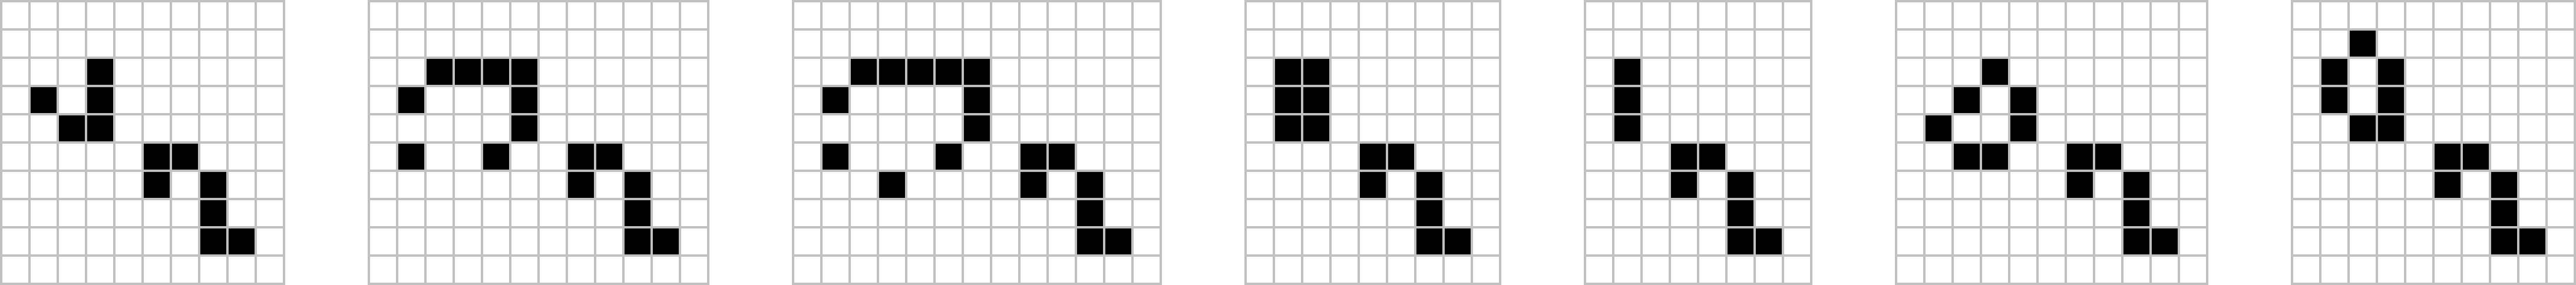
\includegraphics[width=0.9\textwidth]{still_lifes/eater_1_multi.png}}
	\caption{Eater 1 can be used to eat a glider, a lightweight spaceship, a middleweight spaceship, a pre-beehive, and many other objects.}\label{fig:eater_1_multi}
\end{figure}

In spite of the versatility of eater~1, there are other eaters that are sometimes more useful in certain situations. One example is \textbf{eater~2} (see Figure~\ref{fig:eater_2}): although it is quite a bit larger than eater~1 and has a recovery time of 5 generations (instead of 4), it has the advantages of being symmetric and being able to eat gliders traveling along 4 different parallel paths.

Similarly, \textbf{eater~5} (sometimes called the \textbf{tub with tail eater}\index{tub!with tail eater}, or \textbf{TWIT}\index{TWIT|see {tub with tail eater}} for short) is a small eater\footnote{There are indeed eaters called ``eater~3'' and ``eater~4'' (as well as dozens of other known eaters), but they are somewhat less useful than eaters~1, 2, and~5, so we just introduce these others as we need them.} with a recovery time of 6 generations that is made up of two still lifes and is capable of eating gliders traveling along 2 different perpendicular paths. Eater~5 is is especially useful for the fact that it can eat gliders traveling so close to its edge (in particular, the glider coming from the top-right corner in Figure~\ref{fig:eater_5}), so it can often be used to eat gliders in tight places where other eaters will not fit.

\begin{figure}[!htb]
	\begin{subfigure}{.5\textwidth}
		\centering
		\patternimglink{0.083}{eater_2}
		\caption{Eater~2.}
		\label{fig:eater_2}
	\end{subfigure}% 
	\begin{subfigure}{.5\textwidth}
		\centering
		\patternimglink{0.115}{eater_5}
		\caption{Eater~5.}
		\label{fig:eater_5}
	\end{subfigure}
	\caption{Eater~2 (left) is capable of eating gliders traveling along 4 different parallel paths, while eater~5 (right) is capable of eating gliders traveling along 2 different perpendicular paths.}\label{fig:eater_2_5}
\end{figure}


%%%%%%%%%%%%%%%%%%%%%%%%%%%%%%%%%%%%%%%%%%%%%%%%%%%%%%%%%%%%%%%%%%%%%%%%%
%%   SUBSECTION: ROCKS AND ALMOST EATERS
%%%%%%%%%%%%%%%%%%%%%%%%%%%%%%%%%%%%%%%%%%%%%%%%%%%%%%%%%%%%%%%%%%%%%%%%%
\subsection{Rocks and ``Almost'' Eaters}\label{sec:rocks_almost_eaters}

All of the eaters that we have seen so far are temporarily disturbed when the glider hits them, and then return to their initial state after a few generations. However, there is no fundamental reason that an eater has to be disturbed by the object that it eats at all---an eater is called a \textbf{rock} if it does not even suffer temporary damage during the eating process. While there are no known rocks that eat gliders, there are rocks that eat other objects, and there are objects that can act as rocks for \emph{multiple} gliders.

Here we present an example of the latter kind---an object that can destroy two gliders, suffer no damage in the process, yet cannot completely destroy just a single glider. In fact, this object is simply the snake\index{snake}, which is capable of turning a single glider into a boat\index{boat}, which then destroys (and is destroyed by) a second glider coming in from the same direction as the first. This reaction is called the \textbf{boat bit},\index{boat!bit}\footnote{Its name comes from the fact that this reaction can be used to store a single bit of memory. We will explore methods like this one for simulating computation in Chapter~\ref{chp:universal_computation}.} and is displayed in Figure~\ref{fig:boat_bit}.

\begin{figure}[!htb]
	\centering
	\embedlink{boat_bit}{\vcenteredhbox{\patternimg{0.1}{boat_bit_0}} \vcenteredhbox{\genarrow{4}} \vcenteredhbox{\patternimg{0.1}{boat_bit_4}} \vcenteredhbox{\genarrow{20}} \vcenteredhbox{\patternimg{0.1}{boat_bit_24}}}
	\caption{A \textbf{boat-bit} is a reaction in which a snake (or any other still life containing a pre-block) is used to turn a glider into a boat which then destroys a second glider coming in from the same position. Furthermore, the snake is not even temporarily disturbed at any point throughout this reaction.}\label{fig:boat_bit}
\end{figure}

While the snake is not technically an eater since it does not destroy each glider that hits it, but rather only destroys pairs of gliders, this is a technicality that is often unimportant. Typically when eating gliders, an entire stream of gliders (perhaps from a glider gun) are fired from the same position, and this boat-bit reaction gives the smallest known way of erasing such a glider stream (in particular, it contains only $6$ cells and is slightly more compact than the $7$-cell eater~1).

There are also many other reactions that use gliders to toggle a Life object between two or more different states, and they can almost all be used to eat multiple glider streams (though they are often useful for much more than this). For example, a single glider can be used to flip the orientation of a loaf\index{loaf}, so a loaf can use this reaction twice to eat two gliders and end up back where it started, as in Figure~\ref{fig:glider_loaf_flip}. Again, a loaf by itself is not technically an eater since it cannot reconstruct itself after destroying a \emph{single} glider, but we can turn it into an eater by placing a stable object next to it that will flip it back over after a glider hits it. One way of doing this results in the eater called \textbf{eater~3}\index{eater!3}, which is displayed in Figure~\ref{fig:eater_3}.

\begin{figure}[!htb]
	\centering
	\begin{minipage}{.61\textwidth}
		\centering
		\embedlink{glider_loaf_flip}{\vcenteredhbox{\patternimg{0.1}{glider_loaf_flip}} \vcenteredhbox{\genarrow{4}} \vcenteredhbox{\patternimg{0.1}{glider_loaf_flip_4}} \vcenteredhbox{\genarrow{4}} \vcenteredhbox{\patternimg{0.1}{glider_loaf_flip_8}}}
		\caption{A glider can be used to flip a loaf. A loaf can thus be used to eat two gliders coming from opposite directions.}\label{fig:glider_loaf_flip}
	\end{minipage} \quad %
	\begin{minipage}{.33\textwidth}
		\centering
		\patternimglink{0.092899408284}{eater_3}
		\caption{\textbf{Eater 3} is based on the loaf-flipping reaction.}
		\label{fig:eater_3}
	\end{minipage}
\end{figure}

Finally, recall from Section~\ref{sec:queen_bee} that a block\index{block} is the smallest eater of all, as it can be used to eat a beehive (and for that matter, it can also eat a loaf). It can't be used to eat a single glider or even a single glider stream, but it can be used (like a loaf) to eat two gliders coming from opposite directions. This is possible because of the \textbf{(2,1) block pull} reaction\index{(2,1) block pull} displayed in Figure~\ref{fig:glider_block_move}, in which a glider is destroyed while moving a block by $2$ cells horizontally and $1$ cell vertically. A second glider coming from the opposite direction then moves the block back to where it started.

While this reaction is perhaps of limited use when it comes to eating gliders (since the opposing gliders have to be positioned exactly right in order to return the block to its starting point), the general idea of using gliders to move blocks around the Life plane is a very useful one that we will explore in depth in Sections~\ref{sec:slow_salvo} and~\ref{sec:slide_guns}.\footnote{We will also see another use of colliding gliders with a block in Exercise~\ref{exer:rephaser}.}

\begin{figure}[!htb]
	\centering
	\embedlink{glider_block_move}{\vcenteredhbox{\patternimg{0.1}{glider_block_move}} \vcenteredhbox{\genarrow{14}} \vcenteredhbox{\patternimg{0.1}{glider_block_move_14}} \vcenteredhbox{\genarrow{8}} \vcenteredhbox{\patternimg{0.1}{glider_block_move_22}}}
	\caption{A \textbf{(2,1) block pull} is a reaction in which a glider pulls a block by $2$ cells in one direction and $1$ cell in the other. A block can thus be used to eat two gliders coming from opposite directions.}\label{fig:glider_block_move}
\end{figure}


%%%%%%%%%%%%%%%%%%%%%%%%%%%%%%%%%%%%%%%%%%%%%%%%%%%%%%%%%%%%%%%%%%%%%%%%%
%%   SECTION: WELDING STILL LIFES
%%%%%%%%%%%%%%%%%%%%%%%%%%%%%%%%%%%%%%%%%%%%%%%%%%%%%%%%%%%%%%%%%%%%%%%%%
\section{Welded and Constrained Still Lifes}\label{sec:welding}

We saw in Section~\ref{sec:still_life_grammar} that there are many general methods for constructing a wide variety of still lifes of almost any size. We now focus on using these methods to combine multiple still lifes into a single still life that retains the properties of each of its components (such as the ability to eat gliders that are on specific paths)---a process that is called \textbf{welding}.\index{welding}

To give an example of why we might want to weld two still lifes, suppose that we want to erase two gliders that are in the position shown in Figure~\ref{fig:unstable_eater_1s_a}. Since those gliders are so close to each other, there is no way to eat each of them with individual eaters such as eater~1---they will interfere with each other and no longer be stable, as shown in Figure~\ref{fig:unstable_eater_1s_b}.

\begin{figure}[!htb]
	\centering
	\begin{subfigure}{.47\textwidth}
		\centering
		\patternimglink{0.1}{unstable_eater_1s}
		\caption{Two gliders that we would like to eat.}
		\label{fig:unstable_eater_1s_a}
	\end{subfigure} \quad % 
	\begin{subfigure}{.47\textwidth}
		\centering
		\patternlink{unstable_eater_1s}{\patternimg{0.1}{unstable_eater_1s_b}}
		\caption{Placing two individual eaters does not work.}
		\label{fig:unstable_eater_1s_b}
	\end{subfigure}
	\caption{The two gliders in~(a) cannot be eaten by individual eater~1s, since they are too close together and the eater~1s will no longer be stable, as in (b). In particular, the dead cells highlighted in \bgbox{greenback}{green} now have $3$ live neighbors and will be born, while the live cells highlighted in \bgbox{redback}{red} now have $4$ live neighbors and will die. Similar problems occur if we try to use other eaters like eater~2 or eater~5 as well.}\label{fig:unstable_eater_1s}
\end{figure}

To get around this problem, we combine two eater~1s into a single, larger eater. The key idea is that the only part of eater~1 that is actually involved in the glider eating reaction from Figure~\ref{fig:eater_1} is its pre-block (i.e., the $3$-cell corner at its top-left)---its tail is just there to stabilize the pre-block. So to weld two eater~1s together, we place their pre-blocks in the appropriate spots and then replace their tails by a single connecting object in such a way that they are \emph{both} stable, as in Figure~\ref{fig:welded_eater_1s_both}. This stabilizing piece is typically constructed using a combination of the grammar that we introduced in Section~\ref{sec:still_life_grammar} and trial-and-error.

\begin{figure}[!ht]
	\centering
	\begin{subfigure}{.4\textwidth}
		\centering
		\patternimg{0.1}{welded_eater_1s_inc}
		\caption{A placement of pre-blocks (and a bit of the tails) that eats the two gliders.}
		\label{fig:welded_eater_1s_inc}
	\end{subfigure} \quad \ % 
	\begin{subfigure}{.54\textwidth}
		\centering
		\embedlink{welded_eater_1s}{\vcenteredhbox{\patternimg{0.1}{welded_eater_1s}} \vcenteredhbox{\genarrow{4}}
			\vcenteredhbox{\patternimg{0.1}{welded_eater_1s_done}}}
		\caption{A way of welding two eater~1s together to eat both of the gliders.}
		\label{fig:welded_eater_1s}
	\end{subfigure}
	\caption{In order to weld two eater~1s together to make a single still life capable of eating both gliders, we keep both of their pre-blocks but delete their tails, as in (a). We are then free to choose the \bgbox{gridgray!40}{light gray} cells to be alive or dead, and we want to do so in a way that makes the resulting object a still life. One possibility is shown in~(b).}\label{fig:welded_eater_1s_both}
\end{figure}

Welding these two eater~1s together might seem somewhat silly in isolation---we could just place two eater~1s so as to eat the gliders before they get so close together in the first place---but there are two main reasons why welding can be preferable to just placing individual still lifes far apart:\medskip

\begin{enumerate}
	\item[1)] Later on in this book, we will be constructing large patterns that are made up of many other smaller patterns. Some of these sub-patterns might get in our way and restrict the amount of space we have to place the individual still lifes.\smallskip
	
	\item[2)] Similarly, because these large patterns that we will construct are already very large, it is often desirable to reduce their size as much as possible, by packing their components as close together as we can without them colliding. Welding still lifes is one of the main techniques for achieving tight packings of components.\medskip
\end{enumerate}

To give an example that highlights point~(1) above, consider the problem of eating a glider that is positioned as in Figure~\ref{fig:eater_constrained_pre}, but under the restriction that the eater must be contained within the indicated region of the Life plane. Neither eater~1 nor eater~2 come even close to working---if they are positioned in such a way as to eat the glider, they both extend several rows outside of the specified region. However, eater~5 \emph{almost} works---it extends $2$~cells too far in one direction and just $1$~cell too far in the other (see Figure~\ref{fig:eater_constrained_eater_5}).

\begin{figure}[!htb]
	\centering
	\begin{subfigure}{.47\textwidth}
		\centering
		\patternimg{0.1}{eater_constrained_pre}
		\caption{We would like to eat this glider, but our eater must be contained in the \bgbox{gridgray!40}{light gray} region.}
		\label{fig:eater_constrained_pre}
	\end{subfigure} \quad \ % 
	\begin{subfigure}{.47\textwidth}
		\centering
		\patternimg{0.1}{eater_constrained_eater_5}
		\caption{An eater~5 almost works, but sticks just a bit outside of the light gray region.}
		\label{fig:eater_constrained_eater_5}
	\end{subfigure}
	\caption{We are presented with the problem of eating the glider displayed in (a), but under the restriction that the eater we use must live entirely within the light gray region. The only eater that we have seen so far that even comes close to satisfying this restriction is eater~5, so we use that as our starting point in (b).}\label{fig:eater_constrained_eater_5_first}
\end{figure}

To make this eater fit within the specified region, we keep all of the live cells within the region, discard those outside of the region, and then try to add more live cells within the region in order to restore stability and its eating ability. We quickly find that we need to add some live cells to the left and to the bottom-left of the tub in order for the eating reaction to still work.

However, placing live cells near a tub is difficult to do while preserving stability, so we change the tub to a boat and arrive at the pattern in Figure~\ref{fig:eater_constrained_eater_5_b}. This pattern would work as an eater if it were stable, but unfortunately two nearby dead cells come to life in the next generation. To fix this problem, we just extend the pattern to the west and south so as to overpopulate those two cells, until we eventually arrive at a pattern that is completely stable, as in Figure~\ref{fig:eater_constrained_done}. This eater is extremely useful precisely because it eats a glider so close to its corner, and we will make heavy use of it in Section~\ref{sec:herschel_track}.

\begin{figure}[!htb]
	\centering
	\begin{subfigure}{.4\textwidth}
		\centering
		\patternimglink{0.1}{eater_constrained_eater_5_b}
		\caption{An eater that almost works, but is not stable due to the two dead \bgbox{greenback}{green} cells that come to life in the next generation.}
		\label{fig:eater_constrained_eater_5_b}
	\end{subfigure} \quad \ % 
	\begin{subfigure}{.54\textwidth}
		\centering
		\embedlink{eater_constrained_done}{\vcenteredhbox{\patternimg{0.1}{eater_constrained_done}} \vcenteredhbox{\genarrow{6}}
			\vcenteredhbox{\patternimg{0.1}{eater_constrained_done_6}}}
		\caption{We can add additional live cells to the west and south in order to overpopulate the two problematic cells, resulting in an eater that works.}
		\label{fig:eater_constrained_done}
	\end{subfigure}
	\caption{An illustration of one way of transforming eater~5 into an eater that fits within the \bgbox{gridgray!40}{light gray} region. The pattern (a) is not quite stable, since two nearby dead cells come to life in the next generation. The eater depicted in (b) is one solution to this problem, and it has a recovery time of $6$ generations (just like eater~5 itself).}\label{fig:eater_constrained_eater_5_both_done}
\end{figure}


%%%%%%%%%%%%%%%%%%%%%%%%%%%%%%%%%%%%%%%%%%%%%%%%%%%%%%%%%%%%%%%%%%%%%%%%%
%%   SECTION: STILL LIFE DENSITY
%%%%%%%%%%%%%%%%%%%%%%%%%%%%%%%%%%%%%%%%%%%%%%%%%%%%%%%%%%%%%%%%%%%%%%%%%
\section{Still Life Density}\label{sec:still_life_density}

From the very early days of Life, many examples of infinite still lifes were known with density $1/2$. That is, there are many ways of filling the plane in a stable way such that half of the cells are alive and half of them are dead---some examples are presented in Figure~\ref{fig:dense_still_lifes}.
\begin{figure}[!ht]
	\begin{subfigure}{.32\textwidth}
		\centering
		\patternimglink{0.1}{zebra_stripes}
		\caption{\textbf{Zebra stripes}.\index{zebra stripes}}
		\label{fig:zebra_stripes}
	\end{subfigure} \ \ %
	\begin{subfigure}{.32\textwidth}
		\centering
		\patternimglink{0.1}{chicken_wire}
		\caption{\textbf{Chicken wire}.\index{chicken wire}}
		\label{fig:chicken_wire}
	\end{subfigure} \ \ % 
	\begin{subfigure}{.32\textwidth}
		\centering
		\patternimglink{0.1}{onion_rings}
		\caption{\textbf{Onion rings}.\index{onion rings}}
		\label{fig:onion_rings}
	\end{subfigure}
	\caption{When the plane is tiled with these patterns, they create infinite still lifes with density $1/2$.}\label{fig:dense_still_lifes}
\end{figure}

It was a long-standing question whether or not an asymptotic density of greater than $1/2$ is attainable, or if $1/2$ really is the upper limit.\footnote{The conjecture that the asymptotic density of still lifes does not exceed $1/2$ was called the \textbf{still life conjecture}, which was first considered in \emph{Lifeline} vol. 3 in September 1971. In 1992, an upper bound of $6/11$ on the density of an infinite still life was proved by Dean Hickerson using the method outlined in Exercise~\ref{exer:sl_density_611}. This bound was then improved to $15/28$ by Hartmut Holzwart, and finally to $1/2$, hence proving the conjecture, by Noam Elkies in 1998 \cite{Elk98}.} The following theorem shows that the latter is the case: there are no stable configurations that are more dense than those presented in Figure~\ref{fig:dense_still_lifes} (though there are others that also attain density~$1/2$).\footnote{The original proof presented in \cite{Elk98} is somewhat complicated and requires a decent amount of casework, but also finds the maximum asymptotic density of still lifes in many other Life-like cellular automata. The simpler proof provided here, which is specific to the Game of Life, was first presented in \cite{CSB09}.}

\begin{theorem}[Still Life Density (version 1)]\label{thm:still_life_density}
	A still life contained in an $n \times n$ bounding box has no more than $\lfloor n^2/2 \rfloor + 2n$ live cells. In particular, the asymptotic density of still lifes as $n \rightarrow \infty$ is no greater than $1/2$.
\end{theorem}

\begin{proof}
	We prove the theorem by supposing that each cell (either alive or dead) in the Life plane has $2$ tokens, and we will present a procedure for redistributing those tokens among each cell's orthogonal neighbors (i.e., each token stays within its original von Neumann neighborhood) in such a way that every live cell ends up having at least 4 tokens. If we can develop such a procedure, we know that in any $n \times n$ square there will be at most
	$$
	{\color{gray}\underbrace{\color{black}2n^2}_{\substack{\text{original tokens in} \\ \text{$n \times n$ square}}}} \ + \ {\color{gray}\underbrace{\color{black}8n}_{\substack{\text{tokens from $4n$} \\ \text{neighbors of square}}}} = 2(n^2 + 4n) \text{ tokens.}
	$$
	On the other hand, if there are $L$ live cells in an $n \times n$ square, then since every live cell has at least $4$ tokens we know that
	\begin{align*}
		4L & \leq \text{number of tokens on live cells in $n \times n$ square} \\
		& \leq \text{number of tokens on \emph{all} cells in $n \times n$ square} \\
		& \leq 2(n^2 + 4n).
	\end{align*}
	Dividing this inequality by $4$ gives $L \leq n^2/2 + 2n$, which shows that the asymptotic density of a still life cannot exceed $1/2$.
	
	We thus now turn our attention to developing the token redistribution procedure that results in every live square having at least $4$ tokens (thus proving the theorem). The main idea is to have dead cells give away their tokens to neighboring (in the von Neumann neighborhood sense) live cells. The explicit procedure that we use is described in Figure~\ref{fig:density_orthogonal_neighbors}.
	
	\begin{figure}[!htb]
		\centering\begin{tikzpicture}[scale=1.6, every node/.style={transform shape}]%
		\tikzset{
			double arrow/.style args={#1 colored by #2 and #3}{
				round cap-latex,line width=#1,#2, % first arrow
				postaction={draw,round cap-latex,#3,line width=(#1)/3,
					shorten <=(#1)/3,shorten >=2*(#1)/3}, % second arrow
			}
		}
		
		\node[inner sep=0pt,anchor=south west] at (0,0) {
\includegraphics[width=3.3in]{still_lifes/density_orthogonal_neighbors.png}};
		
		\draw[double arrow=4pt colored by white and medgray] (0.755in,0.17in) -- (0.755in,0.04in);
		
		\draw[round cap-latex,line width=4pt,white] (1.355in,0.17in) -- (1.355in,0.04in);
		\draw[round cap-latex,line width=4pt,white] (1.34in,0.155in) -- (1.47in,0.155in);
		\draw[round cap-latex,line width=4/3pt,medgray,shorten <= 4/3pt,shorten >= 8/3pt] (1.355in,0.17in) -- (1.355in,0.04in);
		\draw[round cap-latex,line width=4/3pt,medgray,shorten <= 4/3pt,shorten >= 8/3pt] (1.34in,0.155in) -- (1.47in,0.155in);
		
		\draw[round cap-latex,line width=4pt,white] (1.94in,0.155in) -- (2.07in,0.155in);
		\draw[round cap-latex,line width=4pt,white] (1.94in,0.155in) -- (1.835in,0.155in);
		\draw[round cap-latex,line width=4/3pt,medgray,shorten <= 4/3pt,shorten >= 8/3pt] (1.94in,0.155in) -- (2.07in,0.155in);
		\draw[round cap-latex,line width=4/3pt,medgray,shorten <= 4/3pt,shorten >= 8/3pt] (1.99in,0.155in) -- (1.835in,0.155in);
		
		\draw[round cap-latex,line width=4pt,white] (2.54in,0.155in) -- (2.67in,0.155in);
		\draw[round cap-latex,line width=4pt,white] (2.54in,0.155in) -- (2.435in,0.155in);
		\draw[round cap-latex,line width=4/3pt,medgray,shorten <= 4/3pt,shorten >= 8/3pt] (2.54in,0.155in) -- (2.67in,0.155in);
		\draw[round cap-latex,line width=4/3pt,medgray,shorten <= 4/3pt,shorten >= 8/3pt] (2.59in,0.155in) -- (2.435in,0.155in);
		\end{tikzpicture}
		\caption{All $6$ possible orientations of orthogonal neighbors around a dead cell, up to rotation and reflection---the states of the corner cells in \bgbox{gridgray!40}{light gray} are irrelevant. The \bgbox{medgray!60}{dark gray} arrows indicate where the central dead cell gives its tokens: (a) if it has 1 or 2 live neighbors then it gives one token to each of them, (b) if it has 3 live neighbors then it gives one token to each of the neighbors that are opposite each other, and (c) if it has 0 or 4 live neighbors then it does not give any tokens away.}\label{fig:density_orthogonal_neighbors}
	\end{figure}
	
	We now illustrate how many tokens each live cell in any still life ends up with. To start, we note that every live cell in a still life must have exactly $2$ or $3$ live neighbors, and there are $16$ different configurations of $2$ or $3$ live neighbors around a single live cell, up to rotation and reflection---these $16$ configurations are displayed in Figure~\ref{fig:density_token_input}. It suffices to observe how many tokens the central live cell ends up with in each of these $16$ cases.
	
	\begin{figure}[!htb]
		\centering\begin{tikzpicture}[scale=0.42, every node/.style={transform shape}]%
		\tikzset{
			double arrow/.style args={#1 colored by #2 and #3}{
				round cap-latex,line width=#1,#2, % first arrow
				postaction={draw,round cap-latex,#3,line width=(#1)/3,
					shorten <=(#1)/3,shorten >=2*(#1)/3}, % second arrow
			}
		}
		
		\def\shftx{4.68}
		
		\fill[color=redback] (26.5,-0.5) rectangle (30.5,3.5);
		\fill[color=yellowback] (2.5,-0.5) rectangle (6.5,3.5);
		
		\node[inner sep=0pt,anchor=south west] at (0,0) {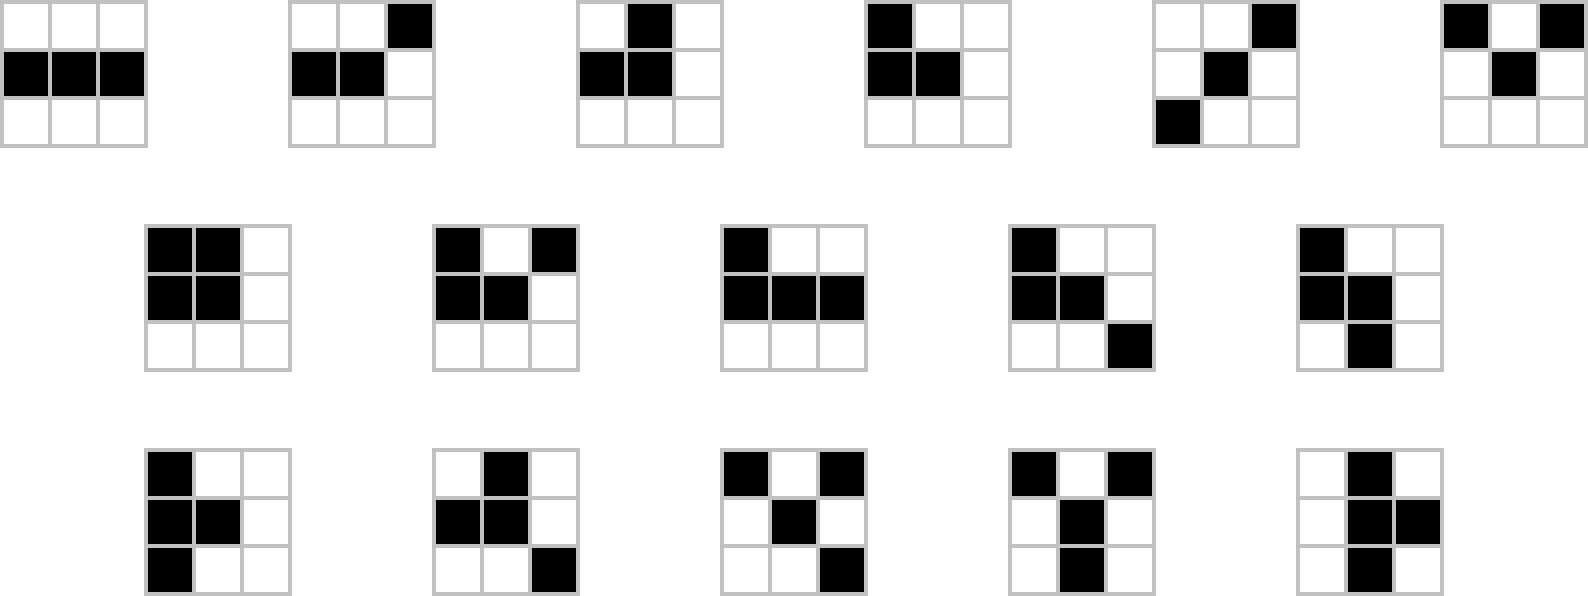
\includegraphics[width=33cm]{still_lifes/density_token_input.png}};
		
		\draw[double arrow=3pt colored by white and medgray] (1.54,12.1+2*\shftx-12) -- (1.54,13.2+2*\shftx-12);
		\draw[double arrow=3pt colored by white and medgray] (1.54,14.9+2*\shftx-12) -- (1.54,13.8+2*\shftx-12);
		\colorletternode{greenback2}{1.54}{1.5+2*\shftx}{4};
		
		\draw[double arrow=3pt colored by white and medgray] (7.54,12.1+2*\shftx-12) -- (7.54,13.2+2*\shftx-12);
		\draw[double arrow=3pt colored by white and medgray] (7.54,14.9+2*\shftx-12) -- (7.54,13.8+2*\shftx-12);
		\draw[double arrow=3pt colored by white and medgray] (8.9,13.54+2*\shftx-12) -- (7.8,13.54+2*\shftx-12);
		\colorletternode{greenback2}{7.54}{1.5+2*\shftx}{5};
		
		\draw[double arrow=3pt colored by white and medgray] (13.55,12.1+2*\shftx-12) -- (13.55,13.2+2*\shftx-12);
		\draw[double arrow=3pt colored by white and medgray] (14.91,13.54+2*\shftx-12) -- (13.81,13.54+2*\shftx-12);
		\colorletternode{greenback2}{13.55}{1.5+2*\shftx}{4};
		
		\draw[double arrow=3pt colored by white and medgray] (19.55,12.1+2*\shftx-12) -- (19.55,13.2+2*\shftx-12);
		\draw[double arrow=3pt colored by white and medgray] (19.55,14.9+2*\shftx-12) -- (19.55,13.8+2*\shftx-12);
		\draw[double arrow=3pt colored by white and medgray] (20.91,13.54+2*\shftx-12) -- (19.81,13.54+2*\shftx-12);
		\colorletternode{greenback2}{19.55}{1.5+2*\shftx}{5};
		
		\draw[double arrow=3pt colored by white and medgray] (25.52,12.1+2*\shftx-12) -- (25.52,13.2+2*\shftx-12); % d to u
		\draw[double arrow=3pt colored by white and medgray] (25.52,14.9+2*\shftx-12) -- (25.52,13.8+2*\shftx-12); % u to d
		\draw[double arrow=3pt colored by white and medgray] (26.88,13.54+2*\shftx-12) -- (25.78,13.54+2*\shftx-12); % r to l
		\draw[double arrow=3pt colored by white and medgray] (24.08,13.54+2*\shftx-12) -- (25.18,13.54+2*\shftx-12); % l to r
		\colorletternode{greenback2}{25.52}{1.5+2*\shftx}{6};
		
		\draw[double arrow=3pt colored by white and medgray] (31.52,12.1+2*\shftx-12) -- (31.52,13.2+2*\shftx-12);
		\draw[double arrow=3pt colored by white and medgray] (32.88,13.54+2*\shftx-12) -- (31.78,13.54+2*\shftx-12);
		\draw[double arrow=3pt colored by white and medgray] (30.08,13.54+2*\shftx-12) -- (31.18,13.54+2*\shftx-12);
		\colorletternode{greenback2}{31.5}{1.5+2*\shftx}{5};
		
		\draw[double arrow=3pt colored by white and medgray] (4.52,6.1+\shftx-6) -- (4.52,7.2+\shftx-6);
		\draw[double arrow=3pt colored by white and medgray] (5.88,7.54+\shftx-6) -- (4.78,7.54+\shftx-6);
		\colorletternode{greenback2}{4.52}{1.5+\shftx}{4};
		
		\draw[double arrow=3pt colored by white and medgray] (10.52,6.1+\shftx-6) -- (10.52,7.2+\shftx-6);
		\draw[double arrow=3pt colored by white and medgray] (11.88,7.54+\shftx-6) -- (10.78,7.54+\shftx-6);
		\colorletternode{greenback2}{10.52}{1.5+\shftx}{4};
		
		\draw[double arrow=3pt colored by white and medgray] (16.52,6.1+\shftx-6) -- (16.52,7.2+\shftx-6); % d to u
		\draw[double arrow=3pt colored by white and medgray] (16.52,8.9+\shftx-6) -- (16.52,7.8+\shftx-6); % u to d
		\colorletternode{greenback2}{16.52}{1.5+\shftx}{4};
		
		\draw[double arrow=3pt colored by white and medgray] (22.52,6.1+\shftx-6) -- (22.52,7.2+\shftx-6); % d to u
		\draw[double arrow=3pt colored by white and medgray] (22.52,8.9+\shftx-6) -- (22.52,7.8+\shftx-6); % u to d
		\draw[double arrow=3pt colored by white and medgray] (23.88,7.54+\shftx-6) -- (22.78,7.54+\shftx-6); % r to l
		\colorletternode{greenback2}{22.49}{1.5+\shftx}{5};
		
		\draw[double arrow=3pt colored by white and medgray] (28.52,8.9+\shftx-6) -- (28.52,7.8+\shftx-6); % u to d
		\draw[double arrow=3pt colored by white and medgray] (29.88,7.54+\shftx-6) -- (28.78,7.54+\shftx-6); % r to l
		\colorletternode{greenback2}{28.49}{1.5+\shftx}{4};
		
		\draw[double arrow=3pt colored by white and medgray] (4.52,0.1) -- (4.52,1.2); % d to u
		\draw[double arrow=3pt colored by white and medgray] (4.52,2.92) -- (4.52,1.82); % u to d
		\draw[double arrow=3pt colored by white and medgray] (5.9,1.54) -- (4.8,1.54); % r to l
		\colorletternode{greenback2}{4.52}{1.5}{5};
		
		\draw[double arrow=3pt colored by white and medgray] (10.52,0.1) -- (10.52,1.2); % d to u
		\draw[double arrow=3pt colored by white and medgray] (11.9,1.54) -- (10.8,1.54); % r to l
		\colorletternode{greenback2}{10.52}{1.5}{4};
		
		\draw[double arrow=3pt colored by white and medgray] (16.52,0.1) -- (16.52,1.2); % d to u
		\draw[double arrow=3pt colored by white and medgray] (15.1,1.54) -- (16.2,1.54); % l to r
		\colorletternode{greenback2}{16.52}{1.5}{4};
		
		\draw[double arrow=3pt colored by white and medgray] (23.9,1.54) -- (22.8,1.54); % r to l
		\draw[double arrow=3pt colored by white and medgray] (21.1,1.54) -- (22.2,1.54); % l to r
		\colorletternode{greenback2}{22.49}{1.5}{4};
		
		\draw[double arrow=3pt colored by white and medgray] (27.1,1.54) -- (28.2,1.54); % l to r
		\colorletternode{greenback2}{28.49}{1.5}{3};
		\end{tikzpicture}
		\caption{All $16$ possible orientations of $2$ or $3$ live neighbors around a live cell, up to rotation and reflection. The \bgbox{medgray!60}{dark gray} arrows indicate which of its neighboring dead cells give tokens to it. The number of tokens that end up on the central live cell is indicated in \bgbox{greenback}{green}, and is always $2$ more than the number of arrows pointing to that cell. The one problematic configuration that results in the central live cell having fewer than $4$ tokens is the one at the bottom-right, outlined in \bgbox{redback}{red}, but it can be fixed with the configuration at the bottom-left, outlined in \bgbox{yellowback2}{yellow}.}\label{fig:density_token_input}
	\end{figure}
	
	We see that in $15$ of the $16$ cases, the live cells ends up having at least $4$ tokens, as desired. However, the configuration at the bottom-right of Figure~\ref{fig:density_token_input} (outlined in red) results in the live cell only having $3$ tokens. To fix this problematic configuration, we claim that it must always be directly to the left of the configuration at the bottom-left of Figure~\ref{fig:density_token_input} (outlined in yellow). To see why this claim is true, notice that the middle-right live cell in the red configuration already has $3$ live neighbors, so the $3$ cells to its immediate right must be dead so as to avoid killing it by overpopulation---in other words, this cell is the central cell in the yellow configuration. In the other direction, notice that the middle-left live cell in the yellow configuration already has $3$ live neighbors, so again the $3$ cells to its immediate left must be dead so as to avoid it dying by overpopulation---in other words, this cell is the central cell in the red configuration.
	
	We have thus shown that the red and yellow configurations always occur together. We can thus simply transfer one of the tokens from the cell with $5$ tokens to the cell with $3$ tokens, resulting in every live cell having at least $4$ tokens (see Figure~\ref{fig:density_token_input_fix}), as desired. Since we have redistributed the tokens in such a way that every live cell now has at least $4$ tokens, and no token has traveled outside of its original von Neumann neighborhood, we are done.
\end{proof}

\begin{figure}[!htb]
	\centering
	\begin{minipage}[b]{0.46\textwidth}
		\centering
		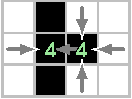
\includegraphics[scale=1.25]{still_lifes/token_redist.pdf}
		\caption{To fix the configuration from Figure~\ref{fig:density_token_input} that results in a live cell only having $3$ tokens, we transfer an extra token from a bordering live cell that has $5$.}\label{fig:density_token_input_fix}
	\end{minipage}\hfill
	\begin{minipage}[b]{0.51\textwidth}
		\centering
		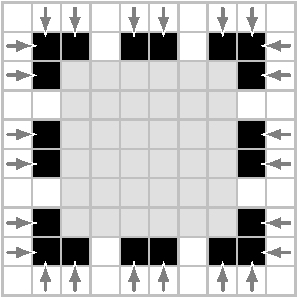
\includegraphics[scale=0.7]{still_lifes/token_dist_border.pdf}
		\caption{This border configuration is the one that causes the largest number of tokens to enter the $n \times n$ square: $4\lceil 2n/3\rceil$ (the $n = 8$ case is illustrated here, so $4\lceil 16/3 \rceil = 24$ tokens enter the square region).}\label{fig:density_border_improve}
	\end{minipage}
\end{figure}

One interesting feature of the proof of Theorem~\ref{thm:still_life_density} is that it tells us which $3 \times 3$ subpatterns of still lifes are the best at being packed densely: the patterns that result in the central cell having exactly $4$ tokens. For example, every single live cell in the infinite still lifes in Figure~\ref{fig:dense_still_lifes} ends up with exactly $4$ tokens. Similarly, it is straightforward to check that the densest still life in a $3 \times 3$ square is the ship\index{ship} (see Table~\ref{tab:still_life_n10}), and every live cell in the ship also ends up with exactly $4$ tokens. By contrast, each live cell in the tub (a less dense $3 \times 3$ still life) ends up with $5$ tokens.

While it is nice to have an answer to the asymptotic version of the still life density problem, Theorem~\ref{thm:still_life_density} does quite poorly at bounding the maximum number of cells in a given (finite) $n \times n$ square. For example, in the $n = 3$ case, that theorem says that a still life cannot have more than $10$ live cells, which is trivially true since a $3 \times 3$ square only has $9$ squares anyway. To improve the bound provided by the theorem, we note that our upper bound on the number of tokens that end up in the $n \times n$ square ($2n^2 + 8n$) can be improved without too much difficulty. In particular, far fewer than $8n$ tokens can actually enter the square from the $4n$ dead cells that neighbor it---this is because our token redistribution procedure never sends both of the tokens from one dead cell in the same direction, so in fact at most $4n$ tokens ($1$ token from each neighboring cell) can enter the square.

In fact, even this bound can be improved, because these $4n$ neighboring dead cells only send a token into the square if their neighbor inside the square is alive. However, only $2$ out of every $3$ cells on the outer edge of the square can be alive, or else they would cause a birth outside of the square and hence not be a still life. It follows that at most $4\lceil 2n/3 \rceil$ tokens can enter the square (see Figure~\ref{fig:density_border_improve}). If we repeat the calculation that was done at the start of the proof of Theorem~\ref{thm:still_life_density}, we immediately arrive at the following result, which is possibly the best upper bound on the density of a finite still life that can be ``easily'' derived:

\begin{theorem}[Still Life Density (version 2)]\label{thm:still_life_density_better}
	A still life contained in an $n \times n$ bounding box has no more than $\lfloor n^2/2 \rfloor + \lceil 2n/3 \rceil$ live cells.
\end{theorem}

For large values of $n$, this new bound is not too much better than the bound provided by Theorem~\ref{thm:still_life_density}, since the $n^2/2$ term is much larger than the $2n$ term that we improved anyway. However, for small values of $n$ this bound is now good enough that it is sometimes exactly correct. In particular, when $n = 2, 3,$ or $5$, this bound equals $4$, $6$, and $16$, respectively, and it is straightforward to construct still lifes that attain these bounds---a block, a ship, and a $2 \times 2$ arrangement of $4$ blocks. For other small squares, we can find the densest still lifes simply by brute-force search: Table~\ref{tab:still_life_n10} gives a summary of the densest patterns in $n \times n$ bounding boxes for $n = 2, 3, 4, \ldots, 10$.

\begin{table}[!htb]\vspace*{0.05in}
	\begin{center}		
		\begin{tabular}{Sc Sc Sl Sc Sc Sc}
			\toprule
			$n$ & \multicolumn{2}{c}{Densest Still Life} & Thm.~\ref{thm:still_life_density_better} Bound & Maximal Live Cells & Density \\\midrule
			\specialcell{2} & \specialcell{\patternimglink{0.1969696969}{densest_block}} & \specialcell{block} & \specialcell{4} & \specialcell{4} & \specialcell{$2/2 = 1.000$} \\
			\rowcolor{gray!20} \specialcell{3} & \specialcell{\patternimglink{0.15853658536}{densest_ship}} & \specialcell{ship} & \specialcell{6} & \specialcell{6} & \specialcell{$6/9 \approx 0.6667$} \\
			\specialcell{4} & \specialcell{\patternimglink{0.13265306122}{densest_pond}} & \specialcell{pond} & \specialcell{11} & \specialcell{8} & \specialcell{$8/16 = 0.5000$} \\
			\rowcolor{gray!20} \specialcell{5} & \specialcell{\patternimglink{0.11403508771}{densest_four_blocks}} & \specialcell{four blocks} & \specialcell{16} & \specialcell{16} & \specialcell{$16/25 = 0.6400$} \\
			\specialcell{6} & \specialcell{\patternimglink{0.1}{densest_6}} & \specialcell{blocks and ship} & \specialcell{22} & \specialcell{18} & \specialcell{$18/36 = 0.5000$} \\
			\rowcolor{gray!20} \specialcell{7} & \specialcell{\patternimglink{0.08904109589}{densest_7}} & \specialcell{--} & \specialcell{29} & \specialcell{28} & \specialcell{$28/49 \approx 0.5714$} \\
			\specialcell{8} & \specialcell{\patternimglink{0.08024691358}{densest_8}} & \specialcell{nine blocks} & \specialcell{38} & \specialcell{36} & \specialcell{$36/64 = 0.5625$} \\
			\rowcolor{gray!20} \specialcell{9} & \specialcell{\patternimglink{0.07303370786}{densest_9}} & \specialcell{--} & \specialcell{46} & \specialcell{43} & \specialcell{$43/81 \approx 0.5309$} \\
			\specialcell{10} & \specialcell{\patternimglink{0.06701030927}{densest_10}} & \specialcell{--} & \specialcell{57} & \specialcell{54} & \specialcell{$54/100 = 0.5400$} \\\bottomrule
		\end{tabular}
		\caption{The densest still lifes that fit within an $n \times n$ bounding box for $2 \leq n \leq 10$, as well as the upper bound on the population of such a still life guaranteed by Theorem~\ref{thm:still_life_density_better}. The examples displayed here are only unique when $n = 2, 3, 5$, or $7$.}\label{tab:still_life_n10}
	\end{center}
\end{table}

Remarkably, we actually know a complete answer to the question of how many live cells a still life in an $n \times n$ bounding box can have. Various clever computer searches were used\footnote{These values for $n \leq 10$ were computed by Robert Bosch in 1999 \cite{Bos99}. This was extended to $n \leq 15$ by Bosch and Michael Trick in 2004 \cite{BT04}, and to $n \leq 20$ by Javier Larrosa, Enric Morancho, and David Niso in 2005 \cite{LMN05}. The remaining values were computed by Geoffrey Chu et. al., with the $n \leq 27$ values being computed in 2009 \cite{CSB09}, and a complete solution for all $n$ being presented in 2012 \cite{CS12}.} to compute the answer when $n \leq 60$, the results of which are summarized in Table~\ref{tab:still_life_n60}. For the $n \geq 61$ cases, the problem stabilizes quite a bit, and there is an explicit formula that is summarized by the following theorem. Proving this theorem is beyond the scope of this book, so the interested reader is directed to \cite{CS12} for details of how it was derived. It is worth noting that the bound we proved in Theorem~\ref{thm:still_life_density_better} is not too far from optimal: the $n^2/2$ term is right, and the linear term in our bound is $2n/3 \approx 0.6667n$, versus the following exact result which has a linear term of $17n/27 \approx 0.6296n$.

\begin{table}[!htb]\vspace*{0.05in}\setlength\arrayrulewidth{0.75pt}
	\begin{center}		
		\begin{tabular}{c | c c c c c c}
			\toprule
			$n$ & $M(n)$ & $M(n+10)$ & $M(n+20)$ & $M(n+30)$ & $M(n+40)$ & $M(n+50)$ \\ \midrule
			$1$ & $0$ & $64$ & $232$ & $497$ & $864$ & $1{\thousep}331$ \\
			\rowcolor{gray!20} $2$ & $4$ & $76$ & $253$ & $531$ & $907$ & $1{\thousep}382$ \\
			$3$ & $6$ & $90$ & $276$ & $563$ & $949$ & $1{\thousep}436$ \\
			\rowcolor{gray!20} $4$ & $8$ & $104$ & $302$ & $598$ & $993$ & $1{\thousep}490$ \\
			$5$ & $16$ & $119$ & $326$ & $633$ & $1{\thousep}039$ & $1{\thousep}545$ \\
			\rowcolor{gray!20} $6$ & $18$ & $136$ & $353$ & $668$ & $1{\thousep}085$ & $1{\thousep}602$ \\
			$7$ & $28$ & $152$ & $379$ & $706$ & $1{\thousep}132$ & $1{\thousep}658$ \\
			\rowcolor{gray!20} $8$ & $36$ & $171$ & $407$ & $744$ & $1{\thousep}181$ & $1{\thousep}717$ \\
			$9$ & $43$ & $190$ & $437$ & $782$ & $1{\thousep}229$ & $1{\thousep}776$ \\
			\rowcolor{gray!20} $10$ & $54$ & $210$ & $467$ & $824$ & $1{\thousep}280$ & $1{\thousep}835$ \\
			\bottomrule
		\end{tabular}
		\caption{A summary of the maximum number of live cells $M(n)$ in a still life with an $n \times n$ bounding box for $1 \leq n \leq 60$.}\label{tab:still_life_n60}
	\end{center}
\end{table}

\begin{theorem}[Still Life Density (version 3)]\label{thm:still_life_density_finite}
	For all $n \geq 61$, the maximum number of live cells $M(n)$ in a still life with an $n \times n$ bounding box is given by the formula
	$$
	M(n) = \begin{cases}
	\lfloor n^2/2 + 17n/27 - 2 \rfloor, & \text{ if } n \equiv 0, 1, 3, 8, 9, 11, 16, 17, 19, 25, 27, \\
	& \quad \quad \ \ \ \, 31, 33, 39, 41, 47, \text{or } 49 \ (\text{mod } 54) , \text{ and} \\
	\lfloor n^2/2 + 17n/27 - 1 \rfloor, & \text{ otherwise}.
	\end{cases}
	$$
\end{theorem}

The related problem of finding the maximum density of an oscillator remains open, even in the (presumably) simpler case of infinite oscillators. Although it is possible for oscillators to have individual phases with density higher than $1/2$ (see Figure~\ref{fig:dense_oscillator} for an example), it seems that their average density over all of their phases is never greater than $1/2$, just like still lifes. Unfortunately, none of the three known proof techniques for the still life case (i.e., the method introduced by Elkies in \cite{Elk98}, the method we used to prove Theorem~\ref{thm:still_life_density}, and the computer-assisted method that was used to prove Theorem~\ref{thm:still_life_density_finite} in \cite{CS12}) seem to carry over in a straightforward way to oscillators.

\begin{figure}[!htb]
	\centering
	\embedlink{dense_oscillator}{\vcenteredhbox{\patternimg{0.1}{dense_oscillator_0}} \vcenteredhbox{\genarrow{1}} \vcenteredhbox{\patternimg{0.1}{dense_oscillator_1}} \vcenteredhbox{\genarrow{1}} \vcenteredhbox{\patternimg{0.1}{dense_oscillator_2}} \vcenteredhbox{\genarrow{1}} \vcenteredhbox{\patternimg{0.1}{dense_oscillator_3}} \vcenteredhbox{\genarrow{1}} \vcenteredhbox{\patternimg{0.1}{dense_oscillator_4}} \vcenteredhbox{\genarrow{1}} \vcenteredhbox{\patternimg{0.1}{dense_oscillator_5}}}
	\caption{A period~$6$ infinite oscillator that has density $3/4$ in two of its phases. However, its average density over all of its phases is $(3/4 + 1/4 + 1/4 + 3/4 + 1/4 + 1/4)/6 = 5/12 \leq 1/2$.}\label{fig:dense_oscillator}
\end{figure}

We could also ask for the densest possible individual phase of an oscillator. It is suspected that the highest possible density is $3/4$, which is attained by some of the phases of the oscillator in Figure~\ref{fig:dense_oscillator}, but no proof of this conjecture has been found either.


%%%%%%%%%%%%%%%%%%%%%%%%%%%%%%%%%%%%%%%%%%%%%%%%%%%%%%%%%%%%%%%%%%%%%%%%%
%%   SECTION: NOTES AND HISTORICAL REMARKS
%%
%%   http://codercontest.com/mniemiec/lifemeth.htm
%%   http://wwwhomes.uni-bielefeld.de/achim/still_life.html
%%%%%%%%%%%%%%%%%%%%%%%%%%%%%%%%%%%%%%%%%%%%%%%%%%%%%%%%%%%%%%%%%%%%%%%%%
\section{Notes and Historical Remarks}\label{sec:still_lifes_notes}
%%%%%%%%%%%%%%%%%%%%%%%%%%%%%%%%%%%%%%%%%%%%%%%%%%%%%%%%%%%%%%%%%%%%%%%%%

Right from the early days of Life, there was considerable interest in cataloging all small still lifes. This process was initiated by John Conway himself, who enumerated the still lifes with $7$ or fewer live cells. Robert Wainwright, with the help of the Life community, then constructed all of them with $10$ or fewer live cells by hand (see Figure~\ref{fig:sl_table_inc}). This effort was soon extended to $12$ cells by Douglas Petrie and Everett Boyer (see Figure~\ref{fig:12_cell_sl_table}). David Buckingham independently went as high as $13$ cells, which we recall there are $240$ of, so cataloging them all by hand (and being sure that none were missed!) was no small feat. Peter Raynham then wrote a search program in the mid-1970s that verified the $13$-cell still life counts and was also used by Buckingham to find all $14$-cell strict still lifes.\index{Lifeline}

\begin{figure}[!htb]
	\centering
	\begin{minipage}[b]{0.48\textwidth}
		\centering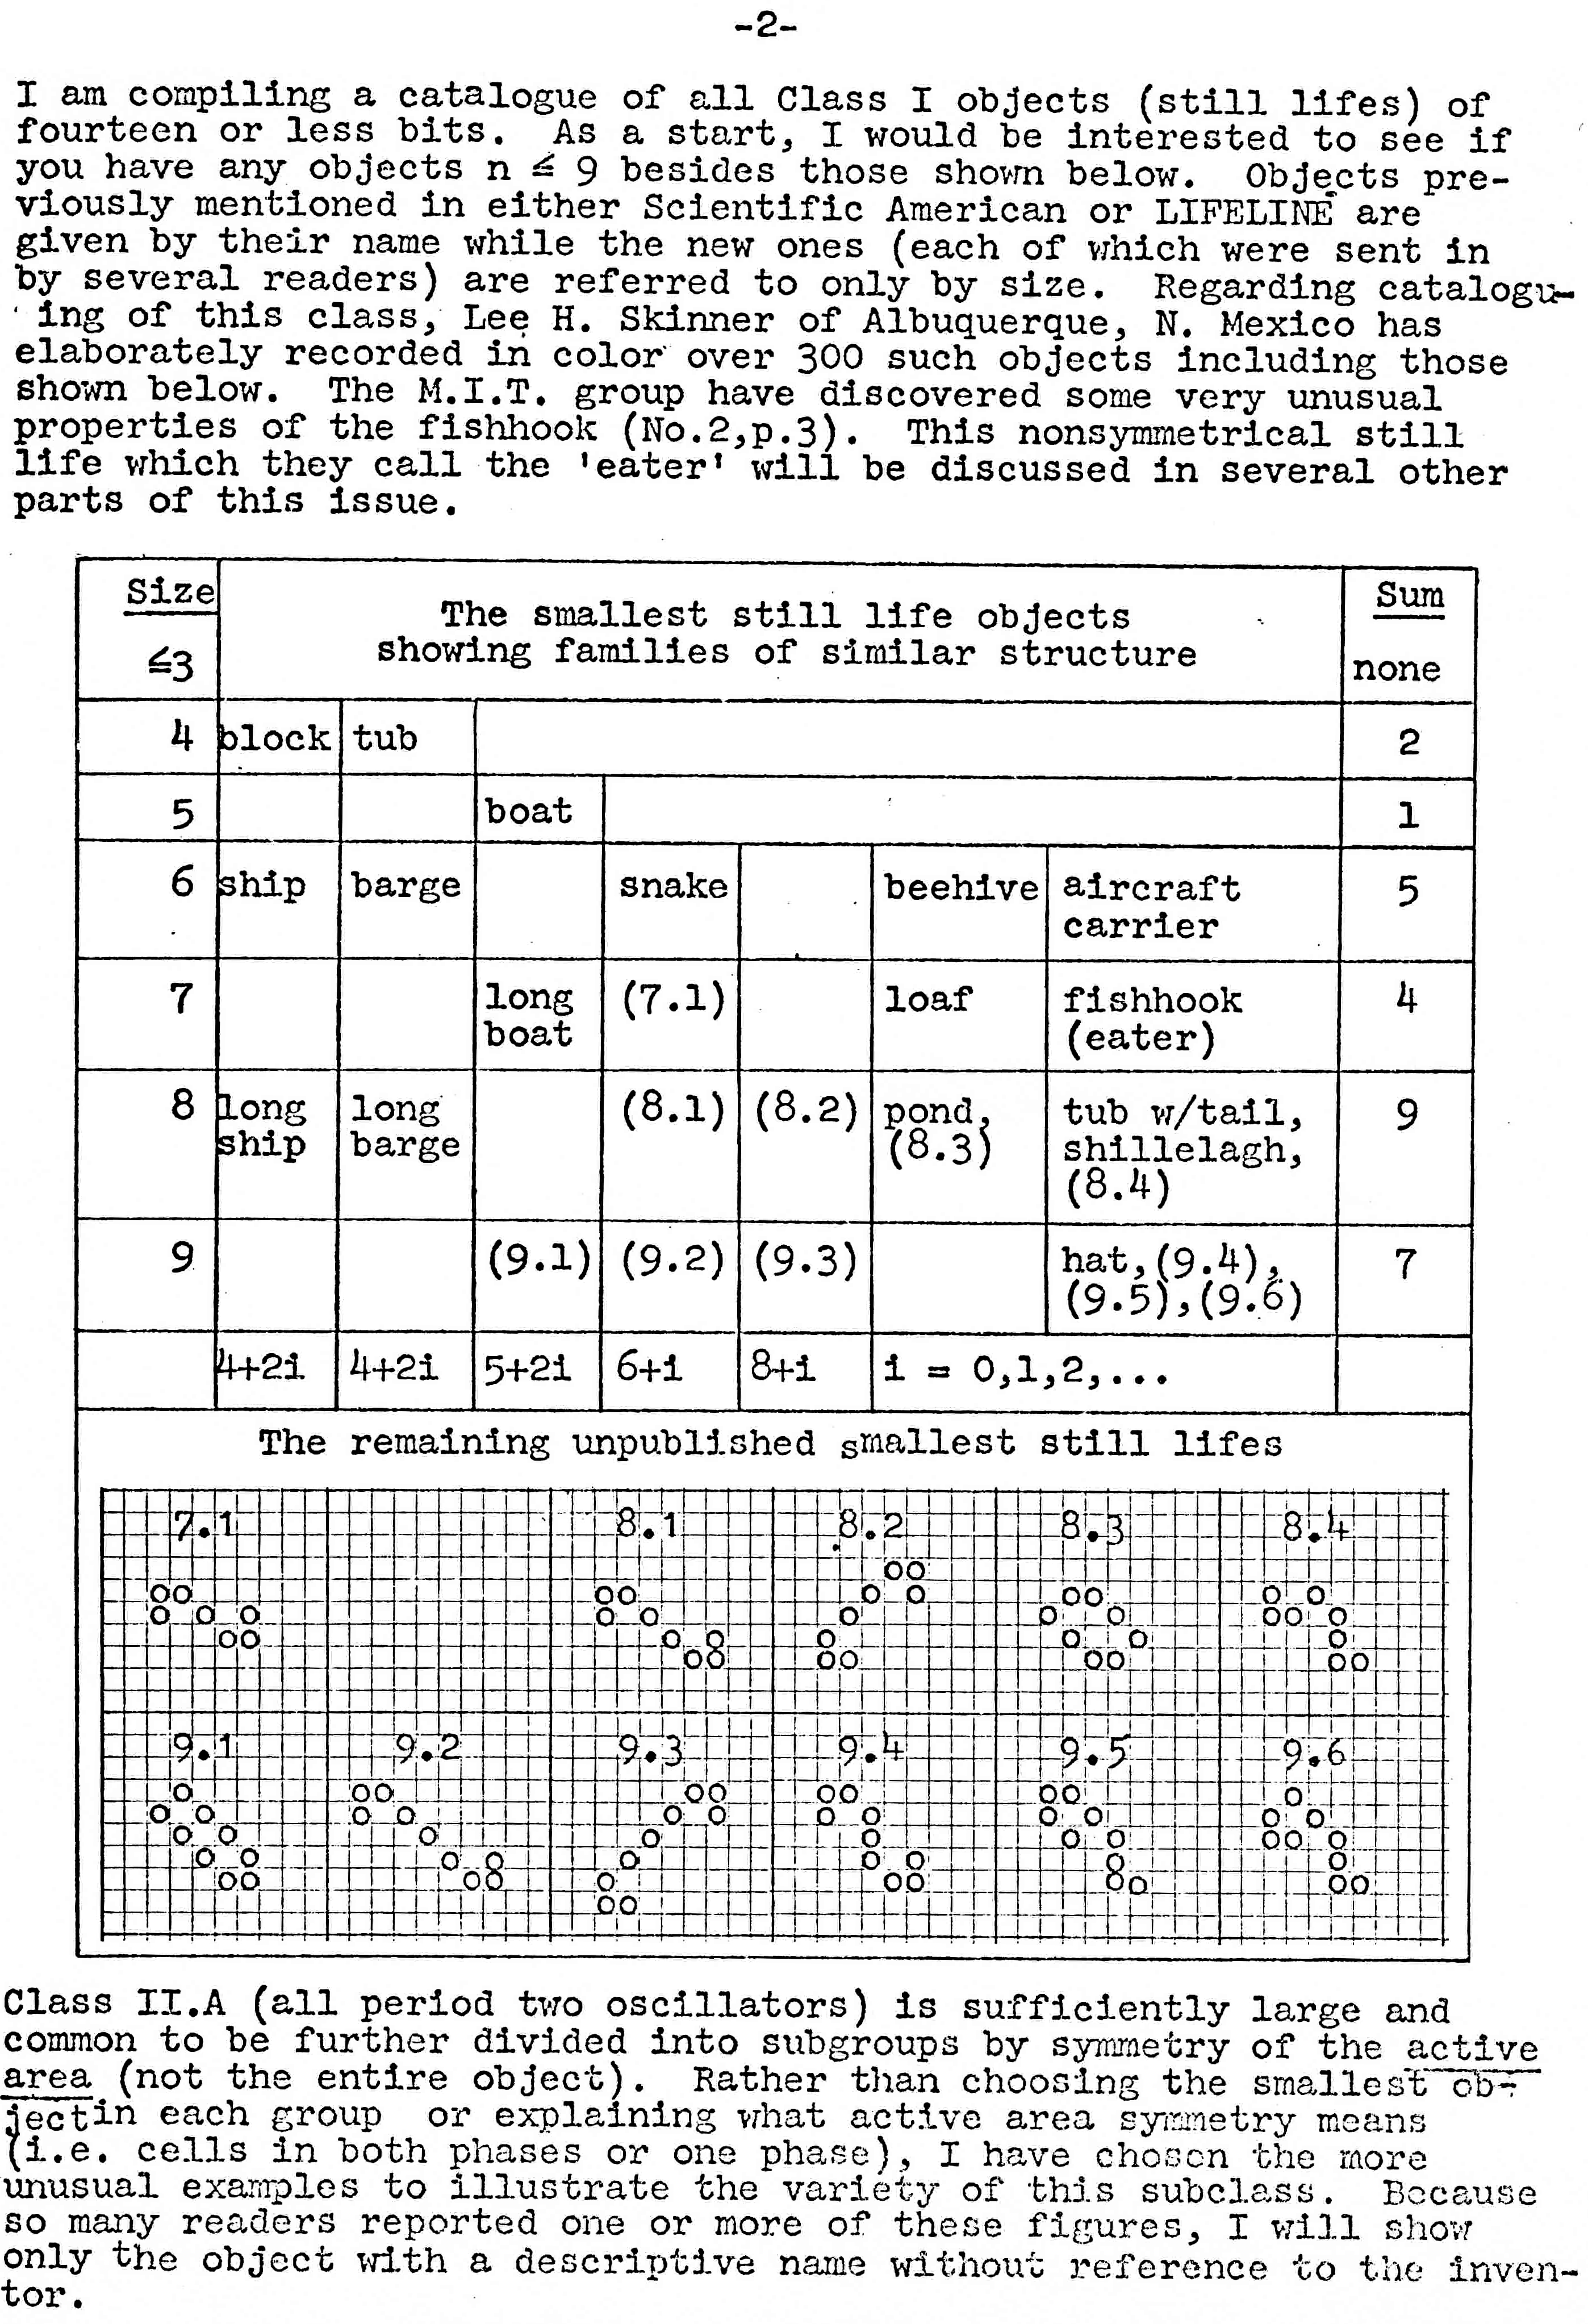
\includegraphics[width=0.75\textwidth]{still_lifes/sl_table_inc.png}
		\caption{A summary of all strict still lifes with $8$ or fewer cells, and an incomplete summary of just $6$ (out of $10$) of the $9$-cell still lifes. Originally published in \emph{Lifeline} vol.~3 in September~1971.}\label{fig:sl_table_inc}
	\end{minipage}\hfill
	\begin{minipage}[b]{0.48\textwidth}
		\centering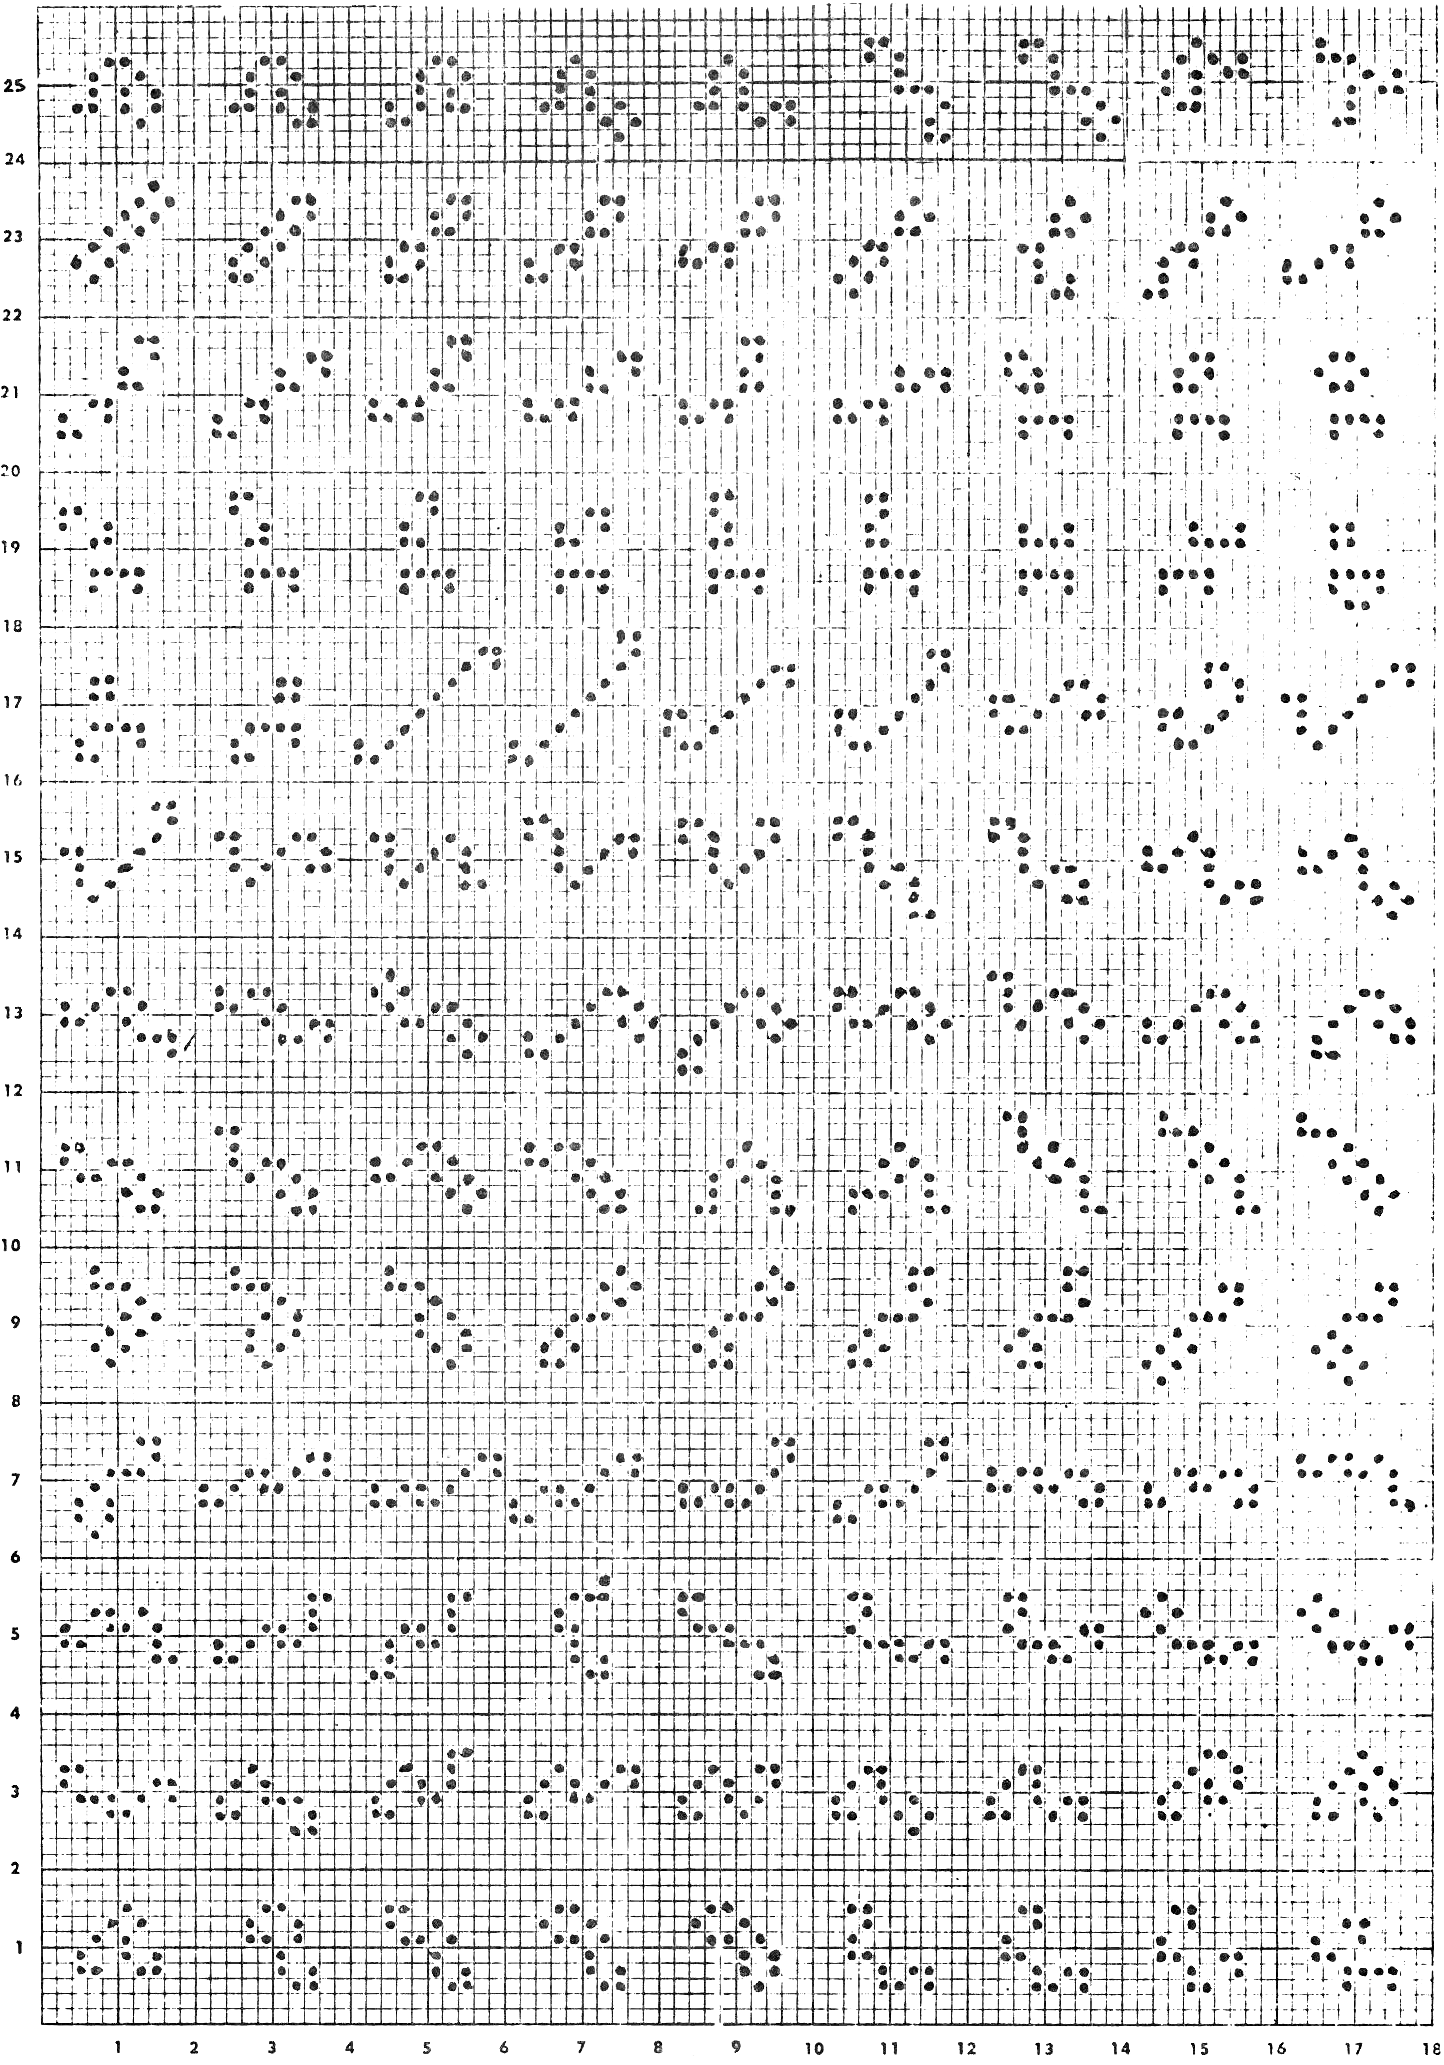
\includegraphics[width=0.75\textwidth]{still_lifes/12_cell_sl_table.png}
		\caption{A summary of all $121$ distinct $12$-cell strict still lifes, compiled by hand by Douglas Petrie and Everett Boyer in 1973. Originally published in \emph{Lifeline} vol.~10 in June~1973.}\label{fig:12_cell_sl_table}
	\end{minipage}
\end{figure}

Much of the early difficulty with counting still lifes with more than $14$ cells came not just from the fact that the search space was large, but also from the fact that even knowing \emph{how} to search for larger still lifes becomes increasingly complicated. To give an idea of why this is the case, suppose we tried to construct strict still lifes by starting at their top-left corner, placing live cells one at a time, checking whether the resulting pattern is stable after each new cell is added. It might seem reasonable to guess that there is no reason to add additional nearby objects once we find a strict still life, since the resulting pattern would then be a pseudo still life. However, this is not actually the case: there are strict still lifes that will never be found if we stop the search when we first find stability, the smallest of which has $16$ cells and is displayed in Figure~\ref{fig:two_tables_on_block}.

\begin{figure}[!htb]
	\centering
	\begin{minipage}{.42\textwidth}
		\centering
		\patternimglink{0.11}{two_tables_on_block}
		\caption{A strict still life that would never be found via a greedy still life search, since a block on table would be found before adding the second table.}\label{fig:two_tables_on_block}
	\end{minipage} \hfill %
	\begin{minipage}{.54\textwidth}
		\centering
		\patternimglink{0.1}{sl_hard_to_find}
		\caption{Two more strict still lifes that won't be found by a greedy still life search, and had to be added by hand when cataloging all still lifes with $22$--$24$ cells.}\label{fig:sl_hard_to_find}
	\end{minipage}
\end{figure}

This problem is not \emph{too} difficult to get around, as there are still only a few different ways that connected components can be near each other, and they can each be coded into the search algorithm individually. For example, objects like the one in Figure~\ref{fig:two_tables_on_block} can be found by allowing the search to add a new domino near an already-stable domino part of the still life. However, each of these tweaks to the algorithm makes it more complicated and thus increases its running time.

Using these ideas, Mark Niemiec conducted a very successful still life search, cataloging all of them with $24$ or fewer live cells by 1999. However, even his searches were not perfect; they missed some still lifes that use a single cell to stabilize a long line of orthogonally-connected cells, like the one in Figure~\ref{fig:sl_hard_to_find}. These still lifes had to be added back into the count by hand, and they were the main reason why he did not extend his search to $25$-cell still lifes---the number of exceptional still lifes that would need to be added back in by hand is too large, and could potentially lead to errors.\footnote{In fact, even after the manual corrections to his $24$-cell still life counts, it was discovered in 2017 that six $24$-cell strict still lifes and one $24$-cell pseudo still life had been missed.}

Finally, Simon Ekström wrote a program to search for still lifes in January 2017 that led to the most successful still life search to date.\footnote{His program is available online at \httpsurl{github.com/simeksgol/GoL_still_life_searcher}} This program has now been used to catalog all still lifes (both strict and pseudo) with $30$ or fewer cells, count all still lifes with $34$ or fewer cells, and also show that the pseudo still lifes from Figure~\ref{fig:pseudo_still_life_decompose} that can be partitioned into $3$ or $4$ still lifes, but not $2$, are the smallest ones possible.


% EXERCISE: Given (3-pseudo or 4-pseudo or 2-pseudo), determine fewest number of partitions into stable sub-pieces. Can use results from recent searches.
%%%%%%%%%%%%%%%%%%%%%%%%%%%%%%%%%
\section*{Exercises \hfill \normalfont\textsf{\small solutions to starred exercises on \hyperlink{solutions_still_lifes}{page \pageref{solutions_still_lifes}}}}
\label{sec:still_lifes_exercises}
\addcontentsline{toc}{section}{Exercises}
\vspace*{-0.4cm}\hrulefill\vspace*{-0.3cm}\footnotesize\begin{multicols}{2}\vspace*{-0.4cm}\raggedcolumns\interlinepenalty=10000
	\setlength{\parskip}{0pt}
	%%%%%%%%%%%%%%%%%%%%%%%%%%%%%%%%%
	
	\begin{problemstar}\label{exer:classify_still_lifes} \probdiff{1}
		Classify each of the following still lifes as either a strict still life, a pseudo still life, or neither.\setlength{\columnsep}{0pt}\vspace*{-0.25cm}
		
		\begin{multicols}{2}
			\begin{enumerate}
				\item[\bf\color{ocre}(a)] \raisebox{-\height+0.5em}{\patternimglink{0.1}{exercise_strict_pseudo_1}}\\[0.2em]
				
				\item[\bf\color{ocre}(c)] \raisebox{-\height+0.5em}{\patternimglink{0.1}{exercise_strict_pseudo_2}}\\[0.9em]
				
				\item[\bf\color{ocre}(e)] \raisebox{-\height+0.5em}{\patternimglink{0.1}{exercise_strict_pseudo_3}}
				
				\item[\bf\color{ocre}(b)] \raisebox{-\height+0.5em}{\patternimglink{0.085}{exercise_strict_pseudo_4}}
				
				\item[\bf\color{ocre}(d)] \raisebox{-\height+0.5em}{\patternimglink{0.085}{exercise_strict_pseudo_5}}
				
				\item[\bf\color{ocre}(f)] \raisebox{-\height+0.5em}{\patternimglink{0.1}{exercise_strict_pseudo_6}}
			\end{enumerate}
		\end{multicols}
	\end{problemstar}
	
	
	\mfilbreak
	
	
	\begin{problem}\label{exer:quasi_still_life} \probdiff{2}
		A \textbf{quasi still life}\index{quasi still life} is a still life that can be partitioned into two or more disjoint still lifes with overlapping Moore neighborhoods (just like pseudo still lifes), but with all cells that stay dead from underpopulation in the constituent still lifes remaining underpopulated in the overall pattern. For example, the cell highlighted in yellow in Figure~\ref{fig:pseudo_not_pseudo} makes that configuration of two blocks a quasi still life.\smallskip
		
		\begin{enumerate}[label=\bf\color{ocre}(\alph*)]
			\item Which of the still lifes from Exercise~\ref{exer:classify_still_lifes} is a quasi still life?
			
			\item Show how to partition the following configuration of $4$ blocks into...
			
			\begin{center}
				\patternlink{densest_four_blocks}{\patternimg{0.1}{densest_four_blocks}}
			\end{center}
			
			\begin{enumerate}[label=\bf\color{ocre}(\roman*)]
				\item two pseudo still lifes,
				
				\item two quasi still lifes, and
				
				\item a quasi still life and two strict still lifes.
			\end{enumerate}
		\end{enumerate}
	\end{problem}
	
	
	\mfilbreak
	
	
	\begin{problemstar}\label{exer:pseudo_few_colors} \probdiff{2}
		Partition each of the following pseudo still lifes into the smallest number (either $2$, $3$, or $4$) of still lifes possible.\setlength{\columnsep}{0pt}\vspace*{-0.25cm}
		
		\begin{multicols}{2}
			\begin{enumerate}[label=(\alph*),series=exer_pseudo]
				\item[\bf\color{ocre}(a)] \raisebox{-\height+0.5em}{\patternimglink{0.1}{exercise_pseudo_1}}
				
				\item[\bf\color{ocre}(c)] \raisebox{-\height+0.5em}{\patternimglink{0.1}{exercise_pseudo_2}}\\[1.0em]
				
				\item[\bf\color{ocre}(e)] \raisebox{-\height+0.5em}{\patternimglink{0.1}{exercise_pseudo_3}}
				
				\item[\bf\color{ocre}(b)] \raisebox{-\height+0.5em}{\patternimglink{0.09}{exercise_pseudo_4}}
				
				\item[\bf\color{ocre}(d)] \raisebox{-\height+0.5em}{\patternimglink{0.085}{exercise_pseudo_5}}
				
				\item[\bf\color{ocre}(f)] \raisebox{-\height+0.5em}{\patternimglink{0.09}{exercise_pseudo_6}}
			\end{enumerate}
		\end{multicols}
	\end{problemstar}
	
	
	\mfilbreak
	
	
	\begin{problemstar}\label{exer:still_life_add_dead} \probdiff{2}
		For each of the following patterns, find a way of changing some nearby dead cells into alive cells so that the resulting pattern is a still life (similarly to how we turned in the path in Figure~\ref{fig:still_life_path} into a still life).\vspace*{-0.25cm}
		
		\begin{multicols}{2}
			\begin{enumerate}
				\item[\bf\color{ocre}(a)] \raisebox{-\height+0.5em}{\patternimglink{0.1}{exercise_path_1}}
				
				\item[\bf\color{ocre}(c)] \raisebox{-\height+0.5em}{\patternimglink{0.1}{exercise_path_2}}
				
				\item[\bf\color{ocre}(b)] \raisebox{-\height+0.5em}{\patternimglink{0.1}{exercise_path_3}}
			\end{enumerate}
		\end{multicols}
	\end{problemstar}
	
	
	\mfilbreak
	
	
	\begin{problem}\label{exer:small_strict_still_lifes} \probdiff{3}
		Find all strict still lifes, distinct up to rotation and reflection, with:\smallskip
		
		\begin{enumerate}[label=\bf\color{ocre}(\alph*)]
			\item $8$ live cells, and
			
			\item $9$ live cells.
		\end{enumerate}
	\end{problem}
	
	
	\mfilbreak
	
	
	\begin{problem}\label{exer:small_pseudo_still_lifes} \probdiff{3}
		Find all pseudo still lifes, distinct up to rotation and reflection, with:\smallskip
		
		\begin{enumerate}[label=\bf\color{ocre}(\alph*)]
			\item $10$ live cells, and
			
			\item $11$ live cells.
		\end{enumerate}
	\end{problem}
	
	
	\mfilbreak
	
	
	\begin{problemstar}\label{exer:still_life_add_coil} \probdiff{2}
		For each of the following patterns, find a way of adding induction coils so as to create a still life.\vspace*{-0.25cm}
		
		\begin{multicols}{2}\setlength{\columnsep}{1pt}
			\begin{enumerate}[label=(\alph*),series=exer_induction_coil]
				\item[\bf\color{ocre}(a)] \raisebox{-\height+0.5em}{\patternimglink{0.1}{exercise_induction_coil_1}}
				
				\item[\bf\color{ocre}(c)] \raisebox{-\height+0.5em}{\patternimglink{0.1}{exercise_induction_coil_2}}
				
				\item[\bf\color{ocre}(b)] \raisebox{-\height+0.5em}{\patternimglink{0.1}{exercise_induction_coil_3}}
			\end{enumerate}
		\end{multicols}
	\end{problemstar}
	
	
	\mfilbreak
	
	
	\begin{problem}\label{exer:gosper_oscillator} \probdiff{1}
		Use the Gosper glider gun and an eater of your choice to create a period~30 oscillator.
	\end{problem}
	
	
	\mfilbreak
	
	
	\begin{problemstar}\label{exer:eater_weld} \probdiff{2}
		For each of the following configurations, weld or modify eater~1s and/or eater~2s so as to create a single eater that can destroy all of the displayed gliders, yet lives entirely within the region specified by the light gray cells.\vspace*{-0.25cm}
		
		\begin{enumerate}
			\begin{multicols}{2}		
				\item[\bf\color{ocre}(a)] \raisebox{-\height+0.5em}{\patternimglink{0.1}{exercise_weld_1}}\vspace*{0.1cm}
				
				\item[\bf\color{ocre}(c)] \raisebox{-\height+0.5em}{\patternimglink{0.1}{exercise_weld_5}}
				
				\item[\bf\color{ocre}(b)] \raisebox{-\height+0.5em}{\patternimglink{0.1}{exercise_weld_2}}
				
				\item[\bf\color{ocre}(d)] \raisebox{-\height+0.5em}{\patternimglink{0.1}{exercise_weld_3}}
			\end{multicols}
		\end{enumerate}
		\begin{enumerate}[label=\bf\color{ocre}(\alph*)]
			\vspace*{-0.32cm}
			\item[\bf\color{ocre}(e)] \raisebox{-\height+0.5em}{\patternimglink{0.1}{exercise_weld_4}}
			
			\item[\bf\color{ocre}(f)] \raisebox{-\height+0.5em}{\patternimglink{0.1}{exercise_weld_6}}\\
		\end{enumerate}
	\end{problemstar}
	
	
	\mfilbreak
	
	
	\begin{problem}\label{exer:eater_2_lwss_mwss} \probdiff{2}
		Show how a single eater~2\index{eater!2} can be used to eat...\smallskip
		
		\begin{enumerate}[label=\bf\color{ocre}(\alph*)]
			\item a lightweight spaceship, and
			
			\item a middleweight spaceship.
		\end{enumerate}
	\end{problem}
	
	
	\mfilbreak
	
	
	\begin{problem}\label{exer:eater_3}
		Recall eater~3\index{eater!3} from Figure~\ref{fig:eater_3}.\smallskip
		
		\begin{enumerate}[label=\bf\color{ocre}(\alph*)]
			\item \probdiff{1} Demonstrate how eater~3 can eat a glider.
			
			\item \probdiff{2} Find at least two still lifes that eater~3 can also eat when they are placed near its loaf.
			
			\item \probdiff{2} Use two copies of the loaf-flipping reaction in eater~3 to create a period~$8$ oscillator.
		\end{enumerate}
		% SOLUTION:
		% x = 100, y = 43, rule = B3/S23
		% 46bobo5bo3bo$45bo3bo4bo3bo4bo$46bo7bo3bo7bo3bo$48b2ob2obo3bob2ob2obo3b
		% o4bo$54bo3bo7bo3bo7bo3bo5bobo$47bo3bo9bo4bo3bob2ob2obo3bo4bo3bo$45bobo
		% 18bo3bo7bo3bo7bo$44bo28bo4bo3bob2ob2o$47bo30bo3bo$44bobo38bo3bo$40bo3b
		% o44bobo$bobo5bo3bo19bo3bo$o3bo4bo3bo4bo9bo4bo3bob2ob2o47bo$bo7bo3bo7bo
		% 3bo7bo3bo7bo45b2o$3b2ob2obo3bob2ob2obo3bob2ob2obo3bo4bo3bo45bo$9bo3bo
		% 7bo3bo7bo3bo5bobo45bo2bo$2bo3bo9bo4bo3bo4bo63bo4bo$obo18bo3bo63b3ob2ob
		% 4o$89b4ob2ob3o$2bo86bo4bo$2b2o90bo2bo$3bo92bo$2bo2bo90b2o$5bo4bo86bo$
		% 3ob2ob4o$4ob2ob3o63bo3bo18bobo$o4bo63bo4bo3bo4bo9bo3bo$5bo2bo45bobo5bo
		% 3bo7bo3bo7bo3bo$7bo45bo3bo4bo3bob2ob2obo3bob2ob2obo3bob2ob2o$7b2o45bo
		% 7bo3bo7bo3bo7bo3bo7bo$8bo47b2ob2obo3bo4bo9bo4bo3bo4bo3bo$62bo3bo19bo3b
		% o5bobo$8bobo44bo3bo$10bo3bo38bobo$17bo3bo30bo$11b2ob2obo3bo4bo28bo$9bo
		% 7bo3bo7bo3bo18bobo$8bo3bo4bo3bob2ob2obo3bo4bo9bo3bo$9bobo5bo3bo7bo3bo
		% 7bo3bo$24bo4bo3bob2ob2obo3bob2ob2o$29bo3bo7bo3bo7bo$36bo4bo3bo4bo3bo$
		% 41bo3bo5bobo!
	\end{problem}
	
	
	\mfilbreak
	
	
	\begin{problem}\label{exer:still_life_impossible} \probdiff{4}
		Prove that it is not possible to stabilize the path of live cells displayed below into a still life, no matter what dead cells you change to alive.
		
		\begin{center}
			\patternimglink{0.1}{exercise_still_life_impossible}
		\end{center}
	\end{problem}
	
	
	\mfilbreak
	
	
	\begin{problemstar}\label{exer:fast_glider_eater} \probdiff{2}
		Show how each of the following still lifes can be used to eat a glider in only $4$ generations, tying them with eater~1 as the fastest-known glider eaters.\vspace*{-0.25cm}
		
		\begin{multicols}{2}
			\begin{enumerate}
				\item[\bf\color{ocre}(a)] \raisebox{-\height+0.5em}{\patternimglink{0.1}{fast_glider_eater}}
				
				\item[\bf\color{ocre}(b)] \raisebox{-\height+0.5em}{\patternimglink{0.1}{fast_glider_eater_b}}
			\end{enumerate}
		\end{multicols}
	\end{problemstar}
	
	
	\mfilbreak
	
	
	\begin{problem}\label{exer:loaf_eater} \probdiff{1}
		Show how a single loaf can eat both of the gliders displayed in Exercise~\ref{exer:eater_weld}(a).
	\end{problem}
	% x = 73, y = 15, rule = B3/S23
	% 2bo19bo$obo17bobo19bo19bo$b2o18b2o17bobo17bobo$25b2o14b2o18b2o$24bo2bo
	% 16b2o$2o22bobo16bo2bo18b2o$2o23bo17bobo18bo2bo$44bo19bobo$30b2o33bo$
	% 30bobo$30bo19b2o$50bobo17b2o$2b3o45bo19bobo$2bo67bo$3bo!
	
	
	\mfilbreak
	
	
	\begin{problemstar}\label{exer:incomplete_glider_eater} \probdiff{3}
		Complete the incomplete glider eater displayed below in such a way that it lives entirely within the region specified by the light gray cells.
		
		\begin{center}
			\patternimg{0.1}{incomplete_glider_eater}
		\end{center}
	\end{problemstar}
	
	
	\mfilbreak
	
	
	\begin{problemstar}\label{exer:still_lifes_6_neigh} \probdiff{3}
		Prove that in a still life, a dead cell can have no more than six live neighbors. Provide an example of a still life that attains this bound.
	\end{problemstar}
	
	
	\mfilbreak
	
	
	\begin{problem}\label{exer:densest_still_lifes} \probdiff{3}
		Find maximum-density still lifes in $n \times n$ bounding boxes for $n = 4, 6,$ and $8$ that are different from those displayed in Table~\ref{tab:still_life_n10}.
	\end{problem}
	
	
	\mfilbreak
	
	
	\begin{problem}\label{exer:still_life_tokens} \probdiff{2}
		In the proof of Theorem~\ref{thm:still_life_density}, we described a procedure for distributing tokens on the Life grid in such a way that every live cell in a still life ends up with at least $4$ tokens. Use this procedure to determine how many tokens end up on each live cell of the following still lifes:\smallskip
		
		\begin{enumerate}[label=\bf\color{ocre}(\alph*)]
			\item block,
			
			\item beehive,
			
			\item pond, and
			
			\item eater~1.
		\end{enumerate}
	\end{problem}
	
	
	\mfilbreak
	
	
	\begin{problemstar}\label{exer:sl_density_611} \probdiff{3}
		In the proof of Theorem~\ref{thm:still_life_density}, we described a procedure for distributing tokens on the Life grid that allowed us to prove that the asymptotic density of still lifes is no greater than $1/2$. If we instead use the much simpler token distribution scheme of ``every dead cell gives each live neighbor (in the Moore neighborhood sense) one token'', then we get a weaker upper bound, which you will now derive.\smallskip
		
		\begin{enumerate}[label=\bf\color{ocre}(\alph*)]
			\item Using this new token distribution scheme, how many tokens should each cell start with to ensure that no cell ends up with a negative number of tokens?
			
			[Hint: Use Exercise~\ref{exer:still_lifes_6_neigh}.]
			
			\item Find a lower bound on the number of tokens that each live cell receives.
			
			\item Mimic the calculation at the start of the proof of Theorem~\ref{thm:still_life_density} to conclude that the asymptotic density of a still life is no greater than $6/11$.
		\end{enumerate}
	\end{problemstar}
	
	
	\mfilbreak
	
	
	\begin{problem}\label{exer:still_life_density_rectangle} \probdiff{4}
		In this question, we consider the problem of finding the maximum density still life in a rectangular $m \times n$ bounding box.\smallskip
		
		\begin{enumerate}[label=\bf\color{ocre}(\alph*)]
			\item Prove that a still life with an $m \times n$ bounding box cannot have more than $\lfloor mn/2 \rfloor + m + n$ live cells.
			
			[Hint: Use the token distribution scheme from the proof of Theorem~\ref{thm:still_life_density}.]
			
			\item Prove that a still life with an $m \times n$ bounding box cannot have more than $$\Big\lfloor mn/2 + \frac{1}{2}\lceil 2m/3 \rceil + \frac{1}{2}\lceil 2n/3 \rceil \Big\rfloor$$ live cells. [Hint: Use the argument that was used to prove Theorem~\ref{thm:still_life_density_better}.]
			
			\item Use the formula from part~(b) to show that a still life with an $2 \times n$ bounding box cannot have more than
			$$
			n + \big\lceil(n+2)/3\big\rceil
			$$
			live cells. Show that this bound is tight whenever $n \geq 2$ and $n \not\equiv 0 \ (\text{mod } 3)$. What do you expect the maximum number of live cells is when $n \equiv 0 \ (\text{mod } 3)$? Prove it.
			% to prove tightness when n \equiv 1 mod 3, use blocks next to each other. When n \equiv 2 mod 3, use snake and snake-like still lifes. when n = 0 mod 3, we expect it equal to n + ceil((n+2)/3) - 1 (i.e., one less than this formula)
			
			\item Write a computer program that calculates the maximum number of live cells in a still life with a $3 \times n$ bounding box for $n = 2, 3, \ldots, 10$. Compare your results with the bound from part~(b).
			% SOLUTION: 4, 6, ...? 
		\end{enumerate}
	\end{problem}
	
	
	\mfilbreak
	
	
	\begin{problem}\label{exer:dense_oscillator} \probdiff{3}
		Construct an (infinitely large) oscillator of period at least $2$ with average density over all of its phases equal to exactly $1/2$.
	\end{problem}
	
	%% EXERCISE END COMMANDS
\end{multicols}
\normalsize\vspace*{0.01cm}
%% DONE EXERCISE END COMMANDS


%%%%%%%%%%%%%%%%%%%%%%%%%%%%%%%%%%%%%%%%%%%%%%%%%%%%%%%%%%%%%%%%%%%%%%%%%
%%   CHAPTER: OSCILLATORS
%%%%%%%%%%%%%%%%%%%%%%%%%%%%%%%%%%%%%%%%%%%%%%%%%%%%%%%%%%%%%%%%%%%%%%%%%

\renewcommand{\chapterfolder}{oscillators/}
\chapterimage{cover/oscillators}
\chapter{Oscillators}\label{chp:oscillators}\index{oscillator}


\vspace*{-0.4in}
\epigraph{That it will never come again is what makes life so sweet.}{Emily Dickinson}
\vspace*{0.4in}


\noindent Recall that an oscillator is a pattern that returns to its initial phase after 2 or more generations, and the smallest number of generations required is its \textbf{period}\index{period}.\footnote{Still lifes could be thought of as oscillators with period~$1$, but in practice (and in this book) the term ``oscillator'' refers to a pattern with period~$2$ or greater.} Some oscillators that we have already seen occurred naturally, such as the blinker, pulsar, and pentadecathlon, and we also constructed some rather unnatural oscillators as well, such as the queen bee shuttle and twin bees shuttle. We have thus seen examples of oscillators with quite a few different periods: $2, 3, 15, 30$, and $46$, and it seems natural to ask whether or not we can ``fill in'' these gaps and find oscillators with any period of our choosing. This is the main goal of this chapter: develop techniques for constructing as wide a variety of oscillators as possible, in the hope of finding one of every single period.

\begin{figure}[!htb]
	\centering
	\begin{subfigure}{.2\textwidth}
		\centering
		\patternimglink{0.128235294118}{bipole}
		\caption{\textbf{bipole}\index{bipole} (p$2$).}
		\label{fig:bipole}
	\end{subfigure} \ \ \ \ % 
	\begin{subfigure}{.2\textwidth}
		\centering
		\patternimglink{0.1}{jam}
		\caption{\textbf{jam}\index{jam} (p$3$).}
		\label{fig:jam}
	\end{subfigure} \ \ \ \ % 
	\begin{subfigure}{.2\textwidth}
		\centering
		\patternimglink{0.112371134021}{mold}
		\caption{\textbf{mold}\index{mold} (p$4$).}
		\label{fig:mold}
	\end{subfigure} \ \ \ \ % 
	\begin{subfigure}{.23\textwidth}
		\centering
		\patternimglink{0.090082644628}{octagon_2}
		\caption{\textbf{octagon 2}\index{octagon 2} (p$5$).}
		\label{fig:octagon_2}
	\end{subfigure}
	\caption{Some more small naturally-occurring (but rare) oscillators that can be found via computer-assisted soup searches. These oscillators were found by (a)~early Lifenthusiasts at M.I.T. in 1970, (b,c)~Achim Flammenkamp in 1988,\protect\footnotemark \ and (d)~Sol Goodman and Arthur Taber in 1971.}\label{fig:natural_but_rare_oscillators}
\end{figure}

\footnotetext{Jam and mold got their names from the fact that they both consist of something on top of a loaf. To remember which is which, notice that the number of letters in their name matches their period.}While most of this chapter will be devoted to techniques for constructing oscillators, to start we note that there are some more oscillators that can be found simply by evolving random soups, as we did in Section~\ref{sec:fumbling}. However, these oscillators are a fair bit less common than those that we saw earlier, and thus are typically only seen in computer-assisted random searches, rather than ones done by hand. A selection of these naturally-occurring (but rare) oscillators is presented in Figure~\ref{fig:natural_but_rare_oscillators}, and we note that we use the shorthand notation ``p$n$'' to stand for ``period $n$''. For example, we often abbreviate expressions like ``period $4$ oscillator'' as ``p$4$ oscillator''.


%----------------------------------------------------------------------------------------
%	SECTION: Billiard Tables
%----------------------------------------------------------------------------------------
\section{Billiard Tables}\label{sec:billiard_tables}

One of the oldest and simplest methods for creating oscillators by hand is to construct a \textbf{billiard table}: an oscillator in which all of the oscillating cells are enclosed entirely within some stable pattern.\footnote{In an oscillator, the cells that oscillate are called its \textbf{rotor} and the cells that stay alive for all generations are called its \textbf{stator}. A billiard table is thus an oscillator that has its rotor enclosed within its stator.} To get an idea for why billiard tables might be a bit easier to create than general oscillators, let's consider the problem of constructing a billiard table where all of the oscillating cells are placed inside a $4 \times 3$ box (see Figure~\ref{fig:billiard_table_start_1}). To make this oscillator work, we have to do two things:\medskip

\begin{enumerate}
	\item[1)] Stabilize the outside of the pattern so that it does not self-destruct outwardly.\smallskip
	
	\item[2)] Place some debris inside the $4 \times 3$ box in such a way that it bounces around inside the box but never destroys it.\medskip
\end{enumerate}

\begin{figure}[!htb]
	\centering
	\begin{subfigure}{.48\textwidth}
		\centering
		\patternimglink{0.1}{billiard_table_start}
		\caption{A $4 \times 3$ box that we would like to stabilize. The first task is to place stable objects around the outside so as to overpopulate the \bgbox{redback}{red cells}.}
		\label{fig:billiard_table_start_1}
	\end{subfigure} \hfill % 
	\begin{subfigure}{.48\textwidth}
		\centering
		\patternlink{billiard_table_start}{\patternimg{0.1}{billiard_table_start_2}}
		\caption{One way of overpopulating the red cells with stable objects. All that remains is to find oscillating debris to place in the inner \bgbox{greenpastel}{green section}.}
		\label{fig:billiard_table_start_2}
	\end{subfigure}
	\caption{A $4 \times 3$ box that we would like to turn into an oscillator. The red cells in~(a) have 3 live neighbors and thus will be alive in the next generation, unless we crowd them with induction coils. One way of crowding them is shown in~(b).}\label{fig:billiard_table_start}
\end{figure}

Since there are only $2^{4 \times 3} = 4{\thousep}096$ different configurations of alive and dead cells that can be placed in a $4 \times 3$ box, if we can carry out both of the tasks outlined above then we will necessarily have an oscillator with period no larger than $4{\thousep}096$ (this period is of course much higher than we expect to actually attain, since it would be a great shock if the inner box actually looped through all possible configurations).

Task~(1) above is typically straightforward to take care of: we can just place induction coils\index{induction coil} around the edges of the pattern to crowd the dead cells that currently have 3 live neighbors (cells in red in Figure~\ref{fig:billiard_table_start_1}), just like we did to create still lifes in Section~\ref{sec:still_life_grammar}. There are typically numerous ways to do this, and they are usually not difficult to find, even by hand. An example is given in Figure~\ref{fig:billiard_table_start_2}, where the outside of the $4 \times 3$ box is stabilized by two blocks and two snakes.

\begin{figure}[!htb]
	\centering
	\begin{subfigure}{.48\textwidth}
		\centering
		\patternimglink{0.1}{hertz_oscillator}
		\caption{\textbf{Hertz oscillator}\index{Hertz oscillator} (p$8$)}
		\label{fig:hertz_oscillator}
	\end{subfigure} \ \ \ \ % 
	\begin{subfigure}{.48\textwidth}
		\centering
		\patternimglink{0.1}{negentropy}
		\caption{\textbf{Negentropy}\index{negentropy} (p$2$)}
		\label{fig:negentropy}
	\end{subfigure}
	\caption{Two billiard table oscillators based on a $4 \times 3$ box. Both of these oscillators were found by John Conway's research group by no later than 1971.}\label{fig:hertz_negen}
\end{figure}

Task~(2) above is a bit more difficult to take care of, but since there are only $4{\thousep}096$ possible configurations, many of which we clearly do not need to consider (such as the configuration with all cells alive), and the $4 \times 3$ box has four-fold symmetry, it actually does not take long to find oscillators by hand (and a computer program could easily be written to check all possibilities). For example, Figure~\ref{fig:hertz_negen} gives two oscillators that can be found in this way.

However, not all boxes are as fruitful as the $4 \times 3$ one was. For example, if we repeat the above procedure with a $5 \times 3$ box, it is still not difficult to stabilize the outside of the box, but there is no way to fill in its center to turn it into an oscillator (see Exercise~\ref{exer:billiard_table_5x3}). For this reason, somewhat more exotic regions than rectangular boxes are often used when constructing billiard tables, some examples of which are given in Figure~\ref{fig:billiard_tables}. Note that these oscillators all use the same stabilization techniques that we learned in Section~\ref{sec:still_life_grammar}: blocks, tubs, and snakes are used as induction coils, and pre-blocks\index{pre-block} and tails\index{tail} are used to stabilize ``corners'' of objects (as at the top of the burloaferimeter in Figure~\ref{fig:burloaferimeter}, on the left and right of the cauldron in Figure~\ref{fig:cauldron}, and on the left and right of the unnamed p$10$ in Figure~\ref{fig:p10_billiard_table}).

\begin{figure}[!htb]
	\centering
	\begin{tabular}{ccc}
		\begin{subfigure}{.31\textwidth}
			\centering
			\patternimglink{0.115286624204}{burloaferimeter}
			\caption{\textbf{Burloaferimeter}\index{burloaferimeter} (p7)}
			\label{fig:burloaferimeter}
		\end{subfigure} &
		\begin{subfigure}{.31\textwidth}
			\centering
			\patternimglink{0.1}{cauldron}
			\caption{\textbf{Cauldron}\index{cauldron} (p8)}
			\label{fig:cauldron}
		\end{subfigure} &
		\begin{subfigure}{.31\textwidth}
			\centering
			\patternimglink{0.1}{p10_billiard_table}
			\caption{unnamed p$10$}
			\label{fig:p10_billiard_table}
		\end{subfigure}
	\end{tabular}
	\caption{Some simple billiard table oscillators that were known right from the early days of Life. They were found by (a)~David Buckingham in 1972, (b)~Don Woods and Robert Wainwright in 1971, and (c)~David Buckingham no later than 1976.}
	\label{fig:billiard_tables}
\end{figure}


%----------------------------------------------------------------------------------------
%	SECTION: Stabilizing Corners
%----------------------------------------------------------------------------------------
\section{Stabilizing Corners}\label{sec:corner_oscillators}

Another method that is frequently used to construct oscillators by hand is to simply place different combinations of known objects and reactions together, such as how we combined blocks with queen bees to create the queen bee shuttle in Section~\ref{sec:queen_bee}. As another example, recall from Section~\ref{sec:eaters} that eater~1 is extremely robust---it can withstand many different types of debris hitting its corner. One possibility for creating an oscillator then would be to use several eater~1s to ``box in'' an area containing some debris, and then that debris would just bounce around in the middle, leaving the eater~1s unharmed. The general idea here is the exact same as it was for billiard tables: create a stable outer area that can contain some debris that is resistant to changes caused by a chaotic central area.

\begin{figure}[!htb]
	\centering
	\begin{minipage}{.48\textwidth}
		\centering
		\patternimglink{0.11}{two_eaters}
		\caption{\textbf{Two eaters}\index{two eaters} is a period~$3$ oscillator found by Bill Gosper in 1971, consisting of two eater~1s eating and rebuilding their corners.}\label{fig:two_eaters}
	\end{minipage} \hfill %
	\begin{minipage}{.48\textwidth}
		\centering
		\patternimglink{0.084777070063}{snacker}
		\caption{\textbf{Snacker}\index{snacker} is a period~$9$ oscillator constructed by Mark Niemiec in 1972 by placing a pentadecathlon in the middle of four eater~1s.}\label{fig:snacker}
	\end{minipage}
\end{figure}

The simplest oscillator that uses this technique is \textbf{two eaters}\index{two eaters}: a period~$3$ oscillator made up of two eater~1s that eat each other's corners and then re-build themselves (see Figure~\ref{fig:two_eaters}). In order to construct less trivial oscillators, we could move the eater~1s away from each other and place some other object between them. In fact, we already used this technique in Exercise~\ref{exer:queen_bee_eater_1} to stabilize a queen bee with an eater~1. Another important oscillator that can be constructed in this way is the \textbf{snacker}\index{snacker}: a period~9 oscillator that is constructed by placing a pentadecathlon in the middle of four eater~1s (see Figure~\ref{fig:snacker}).

Of course, this technique does not work for \emph{all} types of debris and \emph{all} arrangements of eater~1s, but it does not take long to find combinations that do work, even by hand. A wide variety of oscillators whose corners are stabilized by eater~1 are provided in Figure~\ref{fig:eater_1_oscillators}.

\begin{figure}[!htb]
	\centering
	\begin{subfigure}{.3\textwidth}%a
		\centering
		\patternimglink{0.1}{confused_eaters}
		\caption{\textbf{Confused eaters}\index{confused eaters} (p4)}
		\label{fig:confused_eaters}
	\end{subfigure}% 
	\begin{subfigure}{.3\textwidth}%c
		\centering
		\patternimglink{0.081347150259}{roteightor}
		\caption{\textbf{Roteightor}\index{roteightor} (p8)}
		\label{fig:roteightor}
	\end{subfigure}% 
	\begin{subfigure}{.33\textwidth}%g
		\centering
		\patternimglink{0.081347150259}{period_22}
		\caption{\textbf{Jason's p22}\index{Jason's p22}}
		\label{fig:period_22}
	\end{subfigure} \\[0.2in]
	\begin{subfigure}{.3\textwidth}%b
		\centering
		\patternimglink{0.1}{pentoad}
		\caption{\textbf{Pentoad}\index{pentoad} (p5)}
		\label{fig:pentoad}
	\end{subfigure}% 
	\begin{subfigure}{.3\textwidth}%e
		\centering
		\patternimglink{0.093370165745}{dinner_table}
		\caption{\textbf{Dinner table}\index{dinner table} (p12)}
		\label{fig:dinner_table}
	\end{subfigure}% 
	\begin{subfigure}{.33\textwidth}%d
		\centering
		\patternimglink{0.107643312102}{worker_bee}
		\caption{\textbf{Worker bee}\index{worker bee} (p9)}
		\label{fig:worker_bee}
	\end{subfigure} \\[0.2in]
	\begin{subfigure}{.3\textwidth}%f
		\centering
		\patternimglink{0.1}{honey_thieves}
		\caption{\textbf{Honey thieves}\index{honey!thieves} (p17)}
		\label{fig:honey_thieves}
	\end{subfigure}% 
	\begin{subfigure}{.3\textwidth}%i
		\centering
		\patternimglink{0.089519650655}{period_52}
		\caption{unnamed p52}
		\label{fig:period_52}
	\end{subfigure}% 
	\begin{subfigure}{.33\textwidth}%h
		\centering
		\patternimglink{0.10621761658}{period_36}
		\caption{unnamed p36}
		\label{fig:period_36}
	\end{subfigure}
	\caption{Eater~1s can be used to stabilize the corners of several oscillators with a wide variety of periods. These oscillators were found by (a,f)~David Buckingham no later than 1972, (b,e)~Robert Wainwright in 1972, (c)~Jason Summers in 2000, (d)~Bill Gosper in 1977, (g)~Matthias Merzenich in 2014, (h)~David Buckingham in 1977, and (i)~Noam Elkies in 1995. The oscillators~(e), (f), and (h) were the first known oscillators of their respective periods.}
	\label{fig:eater_1_oscillators}
\end{figure}

It is also possible to use patterns other than eater~1 to stabilize the corners of oscillators. For example, eater~2 is capable of eating most types of debris that eater~1 can, so we could replace each eater~1 by an eater~2 in many of the oscillators from Figure~\ref{fig:eater_1_oscillators} without affecting them in a significant way (see Exercise~\ref{exer:eater_1_replace_eater_2_osc}). Some examples of oscillators that really \emph{require} an eater~2, since an eater~1 does not suffice, are presented in Figure~\ref{fig:eater_2_oscillators}.

\begin{figure}[!htb]
	\centering
	\begin{subfigure}{.3\textwidth}
		\centering
		\patternimglink{0.084279475982}{eater_2_p6}
		\caption{unnamed p$6$} % David Buckingham May 1977
		\label{fig:eater_2_p6}
	\end{subfigure}% 
	\begin{subfigure}{.3\textwidth}
		\centering
		\patternimglink{0.1}{eater_2_p12}
		\caption{unnamed p$12$} % Matthias Merzenich December 2015
		\label{fig:eater_2_p12}
	\end{subfigure}% 
	\begin{subfigure}{.36\textwidth}
		\centering
		\patternimglink{0.094146341463}{eater_2_p13}
		\caption{Buckingham's p$13$} % David Buckingham May 1976
		\label{fig:eater_2_p13}
	\end{subfigure}% 
	\caption{Eater~2s can also be used to stabilize the corners of some oscillators. These oscillators were found by David Buckingham in (a)~1977 and (c)~1976, and by (b) Matthias Merzenich in 2015.}
	\label{fig:eater_2_oscillators}
\end{figure}

Furthermore, there is not necessarily any need to use glider eaters to stabilize the corners (for example, we used blocks in the queen bee shuttle in Section~\ref{sec:queen_bee}), nor do we have to use the same pattern in each of the corners. We explore these possibilities more in Section~\ref{sec:hasslers}.


%----------------------------------------------------------------------------------------
%	SECTION: Composite Periods and Sparks
%----------------------------------------------------------------------------------------
\section{Composite Periods and Sparks}\label{sec:composite_periods}

One very simple way to create oscillators with new periods is to place oscillators with smaller periods next to each other in a non-interacting way. For example, if we place a blinker on the same Life plane as a pulsar, the entire configuration does not return to its initial phase until generation $\mathrm{lcm}(2,3) = 6$, even though the individual components only oscillate at periods~$2$ and~$3$. In order to avoid considering ``uninteresting'' combinations of oscillators like this one, it is typically required that an oscillator must have at least one cell that oscillates at its full period in order to be considered non-trivial.\footnote{Every oscillator we have seen so far is non-trivial.}

Somewhat surprisingly, it is in fact sometimes possible to create non-trivial oscillators with composite periods by combining lower-period oscillators. The key to this technique is to combine oscillators that emit \textbf{sparks}:\index{spark} configurations of cells that die when left alone.\footnote{While the term ``spark'' technically refers to any pattern that dies, it is most commonly used to refer to a piece of an oscillator or spaceship that dies and is in a location that is unoccupied during its other phases.} As an example, consider the pentadecathlon,\index{pentadecathlon} which gives off two sparks in one of its phases (see Figure~\ref{fig:pentadecathlon_spark}). These sparks can be erased or manipulated without affecting the subsequent evolution of the pentadecathlon, which makes them very useful to us. For example, if we were able to find another oscillator (with a different period) that also emits a spark, we could place the sparks next to each other in such a way as to make them interact briefly and then die, resulting in a non-trivial oscillator whose period is the least common multiple of the component oscillators.

As an explicit example of how we can construct a non-trivial oscillator via this technique, we can place a (period~$15$) pentadecathlon next to a (period~$9$) snacker.\index{snacker} This oscillator trivially has period $\mathrm{lcm}(15,9) = 45$, but if we are careful about how we place its components, we can cause a small reaction to occur near their sparks just once every 45 generations, thus making the oscillator non-trivial (see Figure~\ref{fig:pentadecathlon_on_snacker}).

\begin{figure}[!htb]
	\centering
	\begin{minipage}[b]{.35\textwidth}
		\centering
		\patternimg{0.098}{pentadecathlon_spark}
		\caption{One phase of the pentadecathlon has two domino sparks (shown in \bgbox{orangeback}{orange}) that immediately die off.}\label{fig:pentadecathlon_spark}
	\end{minipage} \hfill %
	\begin{minipage}[b]{.61\textwidth}
		\centering\embedlink{pentadecathlon_on_snacker}{\vcenteredhbox{\patternimg{0.075}{pentadecathlon_on_snacker}} \vcenteredhbox{\genarrow{1}}
			\vcenteredhbox{\patternimg{0.075}{pentadecathlon_on_snacker_2}}}
		\caption{A pentadecathlon strategically placed next to a snacker makes a non-trivial period~$45$ oscillator, since the two cells shown in \bgbox{greenback}{green} on the right are only alive 1 generation out of every 45.}\label{fig:pentadecathlon_on_snacker}
	\end{minipage}
\end{figure}

Since so many small oscillators have sparks,\footnote{Billiard tables are a notable exception, which makes them somewhat less useful than other oscillators.} this is a fairly straightforward and flexible method for constructing oscillators with small composite periods. However, we will see in later chapters that sparks are also useful for much more, so it will be handy for us to look at a few different types of them in a bit more depth. For this reason, we now start introducing a large assortment of oscillators that provide sparks (called \textbf{sparkers}\index{sparker}).


%----------------------------------------------------------------------------------------
%	SUBSECTION: Types of Sparkers
%----------------------------------------------------------------------------------------
\subsection{Types of Sparkers}\label{sec:sparkers}

The spark that the pentadecathlon emits, which consists of two cells orthogonally connected to each other, is called a \textbf{domino spark}\index{domino spark}. While we already know of two oscillators that give off domino sparks (the other one being the snacker), it will be useful to have a selection of them of various periods. We thus present some domino sparkers of periods~$3$--$8$ in Figure~\ref{fig:domino_sparkers}. Sparks that are far away from the ``body'' of an oscillator are typically much easier to work with, so the oscillators~\ref{fig:ellison_p4} and~\ref{fig:heavyweight_volcano} are often very useful, despite being much larger than the oscillators~\ref{fig:heavyweight_emulator} and~\ref{fig:fumarole} with the same periods.

\begin{figure}[!htb]
	\centering
	\begin{tabular}{ccc}
		\multirow{2}{*}{
			\begin{subfigure}{.34\textwidth}
				\centering\vspace*{-0.35in}
				\patternimglink{0.089}{p3_domino_sparker}
				\caption{unnamed p3 sparker}
				\label{fig:p3_domino_sparker}
			\end{subfigure}
		} &
		\begin{subfigure}{.33\textwidth}
			\centering
			\patternimglink{0.1}{heavyweight_emulator}
			\caption{\textbf{Heavyweight emulator}\index{heavyweight!emulator} (p4)}
			\label{fig:heavyweight_emulator}
		\end{subfigure} &
		\begin{subfigure}{.24\textwidth}
			\centering
			\patternimglink{0.1}{fumarole}
			\caption{\textbf{Fumarole}\index{fumarole} (p5)}
			\label{fig:fumarole}
		\end{subfigure} \\[0.5in]
		& \begin{subfigure}{.33\textwidth}
			\centering
			\patternimglink{0.090513833992}{ellison_p4}
			\caption{\textbf{Ellison's HW emulator} (p4)}
			\label{fig:ellison_p4}
		\end{subfigure} &
		\begin{subfigure}{.24\textwidth}
			\centering
			\patternimglink{0.090513833992}{p6_domino_sparker}
			\caption{unnamed p6 sparker}
			\label{fig:p6_domino_sparker}
		\end{subfigure} \\[0.5in]
		\begin{subfigure}{.34\textwidth}
			\centering
			\patternimglink{0.1}{heavyweight_volcano}
			\caption{\textbf{Heavyweight volcano}\index{heavyweight!volcano} (p5)}
			\label{fig:heavyweight_volcano}
		\end{subfigure} & \begin{subfigure}{.33\textwidth}
			\centering
			\patternimglink{0.090513833992}{hebdarole}
			\caption{\textbf{Hebdarole}\index{hebdarole} (p7)}
			\label{fig:hebdarole}
		\end{subfigure} &
		\begin{subfigure}{.24\textwidth}
			\centering\vspace*{0.75cm}
			\patternimglink{0.12}{figure_eight}
			\caption{\textbf{Figure eight}\index{figure eight} (p8)}
			\label{fig:figure_eight}
		\end{subfigure}
	\end{tabular}
	\caption{A collection of oscillators that emit a domino spark (highlighted in \bgbox{orangeback}{orange}). These oscillators were found by (a,e,g)~Noam Elkies in 1997, (b)~Robert Wainwright in 1980, (c)~Dean Hickerson in 1989, (d)~Scot Ellison in 2010, (f)~Dean Hickerson in 1995 (with improvements to make it smaller by Scot Ellison in 2007), and (h)~Simon Norton in 1970. The p9 snacker and p15 pentadecathlon also emit domino sparks.}
	\label{fig:domino_sparkers}
\end{figure}

Notice that in each of the pentadecathlon, the snacker, and all of the domino sparkers provided in Figure~\ref{fig:domino_sparkers}, the domino spark is parallel to the closest edge of the oscillator that produces it. It is more difficult to construct oscillators that produce a domino spark that points perpendicular to the oscillator's nearest edge, but they do exist, and they are called \textbf{pipsquirters}\index{pipsquirter}. We collect some small pipsquirters in Figure~\ref{fig:pipsquirters}. Note that the figure eight from Figure~\ref{fig:figure_eight} can typically be thought of as both a regular domino sparker and as a pipsquirter, thanks to the multiple orientations of the sparks that it emits.

\begin{figure}[!htb]
	\centering
	\begin{tabular}{@{}ccc@{}}
		\begin{subfigure}{.33\textwidth}
			\centering
			\patternimglink{0.107643312102}{p5_pipsquirter}
			\caption{p5 pipsquirter}
			\label{fig:p5_pipsquirter}
		\end{subfigure} &
		\begin{subfigure}{.30\textwidth}
			\centering
			\patternimglink{0.087564766839}{p6_pipsquirter}
			\caption{p6 pipsquirter}
			\label{fig:p6_pipsquirter}
		\end{subfigure} &
		\begin{subfigure}{.31\textwidth}
			\centering
			\patternimglink{0.093370165745}{p7_pipsquirter}
			\caption{p7 pipsquirter}
			\label{fig:p7_pipsquirter}
		\end{subfigure}
	\end{tabular}
	\caption{Some pipsquirters: oscillators that produce a domino spark (highlighted in \bgbox{orangeback}{orange}) perpendicular to their closest edge. The p5 pipsquirter (a) was found by David Eppstein in April 2003, but is somewhat less useful than the other pipsquirters since its spark is closer to the rest of the oscillator than in the others. The other two were found by Noam Elkies (b)~in 1997, and (c)~in 1999. The p$8$ figure eight from Figure~\ref{fig:figure_eight} can often be used as a pipsquirter.}
	\label{fig:pipsquirters}
\end{figure}
%p21 pipsquirt (sorta): http://conwaylife.com/forums/viewtopic.php?f=2&t=1437&start=50#p26412

The other most commonly-occurring spark is the one that consists of just a single isolated cell, called a \textbf{dot spark}\index{dot spark}. The period~$4$ mold from Figure~\ref{fig:mold} is one example of an oscillator that gives off a dot spark, and the middleweight spaceship from Figure~\ref{fig:lwss_mwss_hwss} is an example of such a spaceship. Some other examples of oscillators that emit this spark are provided in Figure~\ref{fig:dot_sparkers}.

\begin{figure}[!htb]
	\centering
	\begin{tabular}{@{}ccc@{}}
		\begin{subfigure}{.33\textwidth}
			\centering
			\patternimglink{0.1}{fountain}
			\caption{\textbf{Fountain}\index{fountain} (p4)}
			\label{fig:fountain}
		\end{subfigure} & \begin{subfigure}{.32\textwidth}
			\centering
			\patternimglink{0.1}{middleweight_volcano}
			\caption{\textbf{MW volcano}\index{middleweight!volcano} (p5)}
			\label{fig:middlweight_volcano}
		\end{subfigure} & \begin{subfigure}{.3\textwidth}
			\centering\vspace*{0.3cm}
			\patternimglink{0.1}{sparky_p7}
			\caption{\textbf{Beluchenko's p7}\index{Beluchenko's p7}}
			\label{fig:sparky_p7}
		\end{subfigure} \\[0.45in]
		\multirow{2}{*}{\begin{subfigure}{.33\textwidth}
				\centering
				\patternimglink{0.1}{superfountain}
				\caption{\textbf{Superfountain}\index{superfountain} (p4)}
				\label{fig:superfountain}
		\end{subfigure}} & \multirow{2}{*}{\begin{subfigure}{.32\textwidth}
				\centering\vspace*{-0.49cm}
				\patternimglink{0.081538461538}{middleweight_supervolcano}
				\caption{\textbf{MW supervolcano}\index{middleweight!supervolcano} (p5)}
				\label{fig:mw_supervolcano}\index{middleweight!supervolcano}
		\end{subfigure}} & \begin{subfigure}{.3\textwidth}
			\centering\vspace*{0.33cm}
			\patternimglink{0.1}{middleweight_emulator}
			\caption{\textbf{MW emulator}\index{middleweight!emulator} (p4)}
			\label{fig:middleweight_emulator}
		\end{subfigure} \\
		& & \begin{subfigure}{.3\textwidth}
			\centering\vspace*{0.33cm}
			\patternimglink{0.115}{blocker}
			\caption{\textbf{Blocker}\index{blocker} (p8)}
			\label{fig:blocker}
		\end{subfigure} \\[0.57in]
		\begin{subfigure}{.32\textwidth}
			\centering
			\patternimglink{0.1}{rattlesnake}
			\caption{\textbf{Rattlesnake}\index{rattlesnake} (p11)}
			\label{fig:rattlesnake}
		\end{subfigure} & \begin{subfigure}{.33\textwidth}
			\centering
			\patternimglink{0.1}{koks_galaxy}
			\caption{\textbf{Kok's galaxy}\index{Kok's galaxy} (p8)}
			\label{fig:koks_galaxy}
		\end{subfigure} & \begin{subfigure}{.3\textwidth}
			\centering\vspace*{0.09in}
			\patternimglink{0.12537593985}{unix}
			\caption{\textbf{Unix}\index{unix} (p6)}
			\label{fig:unix}
		\end{subfigure}
	\end{tabular}
	\caption{A collection of oscillators that emit a dot spark (highlighted in \bgbox{orangeback}{orange}). These oscillators were found by Dean Hickerson in (a) 1994, (b) 1992, and (h) 2016, Nicolay Beluchenko in (c) 2009 and (d) 2006,  (e)~Dongook Lee in 2019, Robert Wainwright in (f) 1980 and (g)  no later than 1983 (likely in the early 1970s), (i)~Jan Kok in 1971, and (j)~David Buckingham in 1976.}
	\label{fig:dot_sparkers}
\end{figure}

Names like ``middleweight emulator'' and ``heavyweight volcano'' that are used for some of these oscillators refer to the fact that they give off an arrangement of sparks very similar to that of the middleweight and heavyweight spaceships from Figure~\ref{fig:lwss_mwss_hwss}. ``Emulators'' give their sparks off in the row adjacent to the body of the oscillator itself, while ``volcanoes'' emit them with a single row of space in between, and ``supervolcanoes'' emit them with two rows in between. Some supervolcanoes beyond the one from Figure~\ref{fig:mw_supervolcano} are presented in Exercise~\ref{exer:volcanoes}.\index{volcano}\index{supervolcano}

While two dot sparkers cannot be combined with each other to create a non-trivial oscillator (since two dot sparks cannot give the three live neighbors required to give birth to a new cell), they can instead be combined with other types of sparkers. Just like with domino sparkers, we typically prefer oscillators that emit their sparks far away from the rest of the oscillator, so supervolcanoes and the superfountain from Figure~\ref{fig:superfountain} are rather remarkable, despite their large size.

% Ideally, this figure would be one paragraph later.
\begin{figure}[!htb]
	\centering
	\begin{tabular}{@{}cccc@{}}
		\begin{subfigure}{.2\textwidth}
			\centering
			\patternimglink{0.11804511278}{caterer}
			\caption{\textbf{Caterer}\index{caterer} (p$3$)}
			\label{fig:caterer}
		\end{subfigure} &
		\begin{subfigure}{.22\textwidth}
			\centering
			\patternimglink{0.092899408284}{t_nosed_p4}
			\caption{\textbf{T-nosed p4}\index{T-nosed p4}}
			\label{fig:t_nosed_p4}
		\end{subfigure} &
		\begin{subfigure}{.24\textwidth}
			\centering
			\patternimglink{0.1}{p4_thumb}
			\caption{p4 thumb sparker}
			\label{fig:p4_thumb}
		\end{subfigure} &
		\begin{subfigure}{.24\textwidth}
			\centering
			\patternimglink{0.108275862069}{p9_thumb}
			\caption{p9 thumb sparker}
			\label{fig:p9_thumb}
		\end{subfigure}
	\end{tabular}
	\caption{Some (a,b) finger sparkers and (c,d) thumb sparkers, with their sparks highlighted in \bgbox{orangeback}{orange}. These sparkers were found by Dean Hickerson in (a) 1989 and (d) 1998, (b)~Robert Wainwright in 1989, and (c)~David Eppstein  in 2000. Also, octagon~2 from Figure~\ref{fig:octagon_2} is a period~$5$ finger sparker.}
	\label{fig:finger_thumb_sparks}
\end{figure}

In the sparkers that we have seen so far, the spark was always separated from the rest of the oscillator by at least one dead cell. Perhaps surprisingly, sparks can also sometimes be useful even when they are directly connected to the rest of the oscillator, as long as the spark itself is in a location that is unoccupied during the oscillator's other phases. If the spark is connected orthogonally to another live cell then it is called a \textbf{finger spark}\index{finger spark}, and if it is connected diagonally to another live cell then it is called a \textbf{thumb spark}\index{thumb spark}.\footnote{Some sources instead define a finger to be a connected spark that dies after 2~generations (instead of just 1). Neither the caterer nor the T-nosed p$4$ produce finger sparks under this alternate definition.} Some examples of finger and thumb sparkers are presented in Figure~\ref{fig:finger_thumb_sparks}.

It is perhaps less obvious that these finger and thumb sparks can be used to create composite period oscillators, so we present some explicit examples in Figure~\ref{fig:composite_periods}. Since finger and thumb sparks are less accessible than the other sparks that we have seen (i.e., they are closer to the ``body'' of the oscillator), it is often difficult to combine them with each other, so we instead typically combine them with dot or domino sparks.

% Ideally, this figure would be one paragraph later.
\begin{figure}[!htb]
	\centering
	\begin{tabular}{@{}ccc@{}}
		\begin{subfigure}{.31\textwidth}
			\centering
			\patternimglink{0.0942687747}{p20_composite}
			\caption{p$4$ thumb on fumarole (p$20$)}
			\label{fig:p20_composite}
		\end{subfigure} &
		\begin{subfigure}{.31\textwidth}
			\centering
			\patternimglink{0.09}{p33_oscillator}
			\caption{Caterer on rattlesnake (p$33$)}
			\label{fig:p33_oscillator}
		\end{subfigure} &
		\begin{subfigure}{.31\textwidth}
			\centering
			\patternimglink{0.09}{p36_composite}
			\caption{T-nosed p$4$ on snacker (p$36$)}
			\label{fig:p36_composite}
		\end{subfigure}
	\end{tabular}
	\caption{Some oscillators that work by combining finger and thumb sparks with other sparks. Finger sparks can be combined with either dot spark predecessors (as in (b)) or standard domino sparks (as in (c)), but thumb sparks are best paired with domino sparks (as in (a)). In all cases, the cell that oscillates at the full period (thus making the oscillator non-trivial) is highlighted in \bgbox{greenback}{green}.}
	\label{fig:composite_periods}
\end{figure}

It is also worth pointing out that the caterer is particularly useful as a result of having such a small size and period. Not only is it the smallest known period~$3$ oscillator, but its spark is used in the construction of what are currently the smallest known oscillators of period~$21$, $24$, $33$ (Figure~\ref{fig:p33_oscillator}), $39$, $66$, and $93$.

Finally, there are two more types of sparkers that are somewhat less common, but possibly even more useful than the other sparkers that we have seen so far. Some sparkers create a \textbf{duoplet}\index{duoplet} spark (i.e., a spark consisting of two diagonally-connected alive cells\footnote{The term ``duoplet'' technically refers to \emph{any} connected two-cell object, but since the only other connected two-cell object is the domino spark, there is not much chance for ambiguity in using the term to refer to two diagonally-connected cells.}), such as the twin bees shuttle\index{twin bees!shuttle} that we constructed back in Section~\ref{sec:twin_bees}. Another type of spark, which it seems appropriate to call a \textbf{banana spark}\index{banana spark} based on its shape, is emitted by the variant of the queen bee shuttle\index{queen bee!shuttle} (called a \textbf{buckaroo})\index{buckaroo} displayed in Figure~\ref{fig:buckaroo}. Recall that we demonstrated how to construct this oscillator in Exercise~\ref{exer:queen_bee_eater_1}.

\begin{figure}[!htb]
	\centering
	\begin{tabular}{@{}cc@{}}
		\begin{subfigure}{.53\textwidth}
			\centering
			\patternimglink{0.08082872928}{twin_bees_shuttle_spark}
			\caption{Twin bees shuttle making some duoplet sparks}
			\label{fig:twin_bees_shuttle_spark}
		\end{subfigure} &
		\begin{subfigure}{.43\textwidth}
			\centering
			\patternimglink{0.11}{buckaroo}
			\caption{Buckaroo making a banana spark}
			\label{fig:buckaroo}
		\end{subfigure}
	\end{tabular}
	\caption{Some oscillators that emit slightly less common sparks (highlighted in \bgbox{orangeback}{orange}).}
	\label{fig:duoplet_banana_sparks}
\end{figure}

While these sparkers can be used to create higher-period oscillators just like the other sparkers, they are actually particularly useful for another reason: they can reflect a glider, changing its direction by 90 degrees, as illustrated in Figure~\ref{fig:spark_glider_reflect}. We will make extensive use of glider reflectors later in this chapter when we discuss glider loops, and also throughout most of the rest of this book.

\begin{figure}[!htb]
	\centering\embedlink{spark_glider_reflect}{\vcenteredhbox{\patternimg{0.1}{duoplet_reflect_0}} \vcenteredhbox{\genarrow{3}} \vcenteredhbox{\patternimg{0.1}{duoplet_reflect_3}} \vcenteredhbox{\phantom{\phantomarrowc\phantomarrowc}} \vcenteredhbox{\patternimg{0.1}{banana_reflect_0}} \vcenteredhbox{\genarrow{4}} \vcenteredhbox{\patternimg{0.1}{banana_reflect_4}}}
	\caption{Duoplet and banana sparks can be used to reflect gliders by 90 degrees.}\label{fig:spark_glider_reflect}
\end{figure}


%----------------------------------------------------------------------------------------
%	SECTION: Hasslers
%----------------------------------------------------------------------------------------
\section{Hasslers and Shuttles}\label{sec:hasslers}

In many of the oscillators that we saw in the previous section, the debris that was bounced around between the eaters was recognizable. For example, the dinner table\index{dinner table} in Figure~\ref{fig:dinner_table} bounces around a pre-beehive\index{pre-beehive}, the honey thieves\index{honey!thieves} in Figure~\ref{fig:honey_thieves} bounce around a pre-honey farm\index{pre-honey farm} (hence its name), the oscillator in Figure~\ref{fig:period_36} stabilizes two T-tetrominoes\index{T-tetromino}, and the eaters in Figure~\ref{fig:period_52} stabilize lumps of muck\index{lumps of muck}.

This observation suggests that it might be fruitful to look for oscillators in which the debris in the middle is one of the ``standard'' unstable evolutionary sequences. With this in mind, we say that one pattern \textbf{hassles} another one if it repeatedly moves or changes it, typically in a periodic way so as to create an oscillator or gun. Oscillators created in this way are called \textbf{hasslers}\index{hassler}. In the special case when a hassler moves an object back and forth between two positions (such as the queen bee shuttle from Section~\ref{sec:queen_bee}), it is called a \textbf{shuttle}\index{shuttle}.


%----------------------------------------------------------------------------------------
%	SUBSECTION: Types of Hasslers
%----------------------------------------------------------------------------------------

\subsection{Types of Hasslers}\label{sec:hassler_types}

One of the objects that has proved most effective at being hassled in order to create oscillators is the pre-honey farm (which we first investigated back in Section~\ref{sec:evolution}). The honey thieves oscillator in Figure~\ref{fig:honey_thieves} shows how it can be hassled to create a period~$17$ oscillator, and several more honey farm hasslers are presented in Figure~\ref{fig:honeyfarm_hasslers}. While some of these oscillators were found by hand, such as the one in Figure~\ref{fig:p18_honey_farm}, they are more commonly found via computer searches that try numerous placements of honey farms between various arrangements of small still lifes and sparkers.

\begin{figure}[!htb]
	\centering
	\begin{tabular}{@{}cccc@{}}
		\begin{subfigure}{.16\textwidth}
			\centering
			\embedlink{honeyfarm_hasslers}{\patternimg{0.090960451977}{p16_honey_farm}}
			\caption{period~16}
			\label{fig:p16_honey_farm}
		\end{subfigure} &
		\begin{subfigure}{.235\textwidth}
			\centering
			\patternlink{honeyfarm_hasslers}{\patternimg{0.1}{p18_honey_farm}}
			\caption{period~18}
			\label{fig:p18_honey_farm}
		\end{subfigure} &
		\begin{subfigure}{.245\textwidth}
			\centering
			\patternlink{honeyfarm_hasslers}{\patternimg{0.1}{p21_honey_farm}}
			\caption{period~21}
			\label{fig:p21_honey_farm}
		\end{subfigure} &
		\begin{subfigure}{.25\textwidth}
			\centering
			\patternlink{honeyfarm_hasslers}{\patternimg{0.1}{p32_honey_farm}}
			\caption{period~32}
			\label{fig:p32_honey_farm}
		\end{subfigure}
	\end{tabular}
	\caption{Several oscillators that work by hassling pre-honey farms (highlighted in \bgbox{orangeback}{orange}). These oscillators were found by (a,c)~Dongook Lee in 2016, (b)~Nico Brown in January 2015, and (d)~David Raucci and Aidan F.~Pierce in September 2021.}
	\label{fig:honeyfarm_hasslers}
\end{figure}
% http://conwaylife.com/forums/viewtopic.php?f=2&t=279&start=875#p16048
% p35,45: http://conwaylife.com/forums/viewtopic.php?f=2&t=1437&hilit=hassler&start=75#p26565
% full collection: http://conwaylife.com/forums/viewtopic.php?f=2&t=1437&start=75#p26587

Another common type of hassler is based on the pi-heptomino\index{pi-heptomino} that we introduced in Section~\ref{sec:evolution}. There are some known formations of still lifes and oscillators that can rotate pi-heptominoes by 90 degrees when placed nearby, so using multiple copies of these reactions results in an oscillator. There are also some configurations of stable patterns that can be used to tame the debris produced by a pi-heptomino, causing it to re-form in another location. Some examples of oscillators that work via these mechanisms are presented in Figure~\ref{fig:pi_hasslers}. Note that the one displayed in Figure~\ref{fig:tanners_p46} is particularly useful due to how sparky it is and the fact that it has the same period ($46$) as the twin bees shuttle. We devote the entirety of Section~\ref{sec:p46_tanner} to investigating things that can be done with it.

\begin{figure}[!htb]
	\centering
	\begin{tabular}{@{}ccc@{}}
		\begin{subfigure}{.3\textwidth}
			\centering\vspace*{0.39cm}
			\patternimglink{0.11}{p32_pi_hassler}
			\caption{\textbf{gourmet}\index{gourmet} (p$32$)}
			\label{fig:p32_pi_hassler}
		\end{subfigure} &
		\begin{subfigure}{.37\textwidth}
			\centering
			\patternimglink{0.08}{p37_pi_hassler}
			\caption{p37 pi-heptomino hassler}
			\label{fig:p37_pi_hassler}
		\end{subfigure} &
		\begin{subfigure}{.27\textwidth}
			\centering\vspace*{1.05cm}
			\patternimglink{0.12}{tanners_p46}
			\caption{\textbf{Tanner's p46}\index{Tanner's p46}}
			\label{fig:tanners_p46}
		\end{subfigure}
	\end{tabular}
	\caption{Some oscillators that work by hassling pi-heptominoes (highlighted in \bgbox{orangeback}{orange}). These oscillators were found by (a) David Buckingham in 1978, (b)~Nicolay Beluchenko in 2010, and (c) Tanner Jacobi in 2017. While the oscillator in (b) might not look like it is hassling pi-heptominoes, the chaotic objects the middle are in fact each the 9th generation of the pi-heptomino.}
	\label{fig:pi_hasslers}
\end{figure}

In the examples that we have seen so far, the object being hassled (a pre-honey farm or a pi-heptomino) was unstable, but it does not need to be---it is entirely possible to construct new oscillators by hassling still lifes. In particular, sparks from sparkers can sometimes be used to cause a collection of still lifes to temporarily explode, but then settle back into their original formation. One example of such a hassler is given in Figure~\ref{fig:p27_hassler}, where a dot spark is used to hassle an arrangement of two ponds and two blocks, letting us create a fairly wide variety of oscillator periods. In particular, it takes $20$~generations for these blocks and ponds to return to their original formations, so this reaction can be used to double the period of a sparker with period $10$--$19$ or triple the period of a sparker with period $7$--$9$.

Another example of a still life hassler, called \textbf{David Hilbert},\index{David Hilbert}\footnote{This was the first p$23$ oscillator found. Its name is a reference to the famous mathematician of the same name who published a list of $23$ important unsolved (at that time) mathematical problems in 1900.} is presented in Figure~\ref{fig:david_hilbert} (though it is perhaps more of a shuttle than just a hassler). In this oscillator, two B-heptominoes are hassled so that they then shuttle a beehive back and forth between two positions.

\begin{figure}[!htb]
	\centering
	\begin{subfigure}{.52\textwidth}
		\centering
		\patternimglink{0.1}{p27_hassler}
		\caption{p$27$ still life hassler}
		\label{fig:p27_hassler}
	\end{subfigure} \hfill % 
	\begin{subfigure}{.44\textwidth}
		\centering
		\patternimglink{0.107111111111}{david_hilbert}
		\caption{David Hilbert (p$23$)}
		\label{fig:david_hilbert}
	\end{subfigure}
	\caption{Some oscillators that work by hassling still lifes (highlighted in \bgbox{orangeback}{orange}). These oscillators were found by (a) Jason Summers in 2005 and (b) Luka Okanishi in 2019.}\label{fig:still_life_hassler}
\end{figure}


\subsection{Types of Shuttles}\label{sec:shuttle_types}

We have already seen that queen bees and twin bees can be used to construct period~$30$ and period~$46$ shuttles, but these objects do not really highlight the variety of shuttle oscillators that exist. To give a slightly more exotic example, recall the T-tetromino\index{T-tetromino} that we saw back in Figure~\ref{fig:t_tetromino}. Unlike the pre-honey farms and pi-heptominoes that we just learned can be hassled by still lifes, T-tetrominoes are typically hassled by oscillators (sparkers in particular).\footnote{The most well-known exception being the oscillator in Figure~\ref{fig:period_36}, which uses two eater~1s to hassle two T-tetrominoes.} This is because many common sparks can be used to reposition a T-tetromino, such as the one demonstrated in Figure~\ref{fig:t_tetromino_hassle_1}.

\begin{figure}[!htb]
	\centering
	\embedlink{t_tetromino_hassle_1}{\vcenteredhbox{\patternimg{0.1}{t_tetromino_hassle_1_0}} \vcenteredhbox{\genarrow{5}}
		\vcenteredhbox{\patternimg{0.1}{t_tetromino_hassle_1_5}} \vcenteredhbox{\genarrow{6}} \vcenteredhbox{\patternimg{0.1}{t_tetromino_hassle_1_11}}}
	\caption{A dot spark (highlighted in \bgbox{orangeback}{orange}) can be used to hassle a T-tetromino, moving it to the left by $2$ cells and mirroring it over the course of $11$~generations---resulting in the eventual pre-traffic-light descendant being pushed $3$ cells to the left.}\label{fig:t_tetromino_hassle_1}
\end{figure}

It would be theoretically possible to use this reaction together with two period~$11$ dot sparkers to create a period~$22$ T-tetromino shuttle oscillator, but unfortunately there is no known period~$11$ dot sparker whose spark is emitted far enough away from the oscillator to work.\footnote{The p$11$ rattlesnake\index{rattlesnake} gives a dot spark, but there is no way to place the dot spark in such a way that the T-tetromino avoids colliding with the rattlesnake.} However, one nice feature of shuttles is that we can mix-and-match different shuttling reactions, as long as the distances that they offset the central object (the T-tetromino in this case) are the same. For example, we can couple the previous hassling reaction with the one displayed in Figure~\ref{fig:t_tetromino_hassle_2}, which moves a T-tetromino by the same amount, but only takes $9$~generations (rather than $11$) to do it.

\begin{figure}[!htb]
	\centering
	\embedlink{t_tetromino_hassle_2}{\vcenteredhbox{\patternimg{0.1}{t_tetromino_hassle_2_0}} \vcenteredhbox{\genarrow{3}}
		\vcenteredhbox{\patternimg{0.1}{t_tetromino_hassle_2_4}} \vcenteredhbox{\genarrow{2}} \vcenteredhbox{\patternimg{0.1}{t_tetromino_hassle_2_6}} \vcenteredhbox{\genarrow{4}} \vcenteredhbox{\patternimg{0.1}{t_tetromino_hassle_2_10}}}
	\caption{Three dot sparks (highlighted in \bgbox{orangeback}{orange}) can be used to hassle generation~$1$ of a T-tetromino (i.e., the $7$-cell object on the far left), moving it to the left by $2$ cells and mirroring it over the course of $9$~generations.}\label{fig:t_tetromino_hassle_2}
\end{figure}

By combining these two reactions to move a T-tetromino back and forth, it now takes a total of $11 + 9 = 20$ generations to return to its original position. Fortunately, we have seen some p$4$ and p$5$ sparkers that can create the dot sparks needed to perform the hassling. A period~$20$ T-tetromino shuttle that uses these two shuttle reactions (assisted by a period~$5$ middleweight volcano\index{middleweight!volcano} and three period~$4$ middleweight emulators\index{middleweight!emulator} that have been welded together) is displayed in Figure~\ref{fig:p20_t_tetromino_hassler}.

\begin{figure}[!htb]
	\centering
	\begin{tabular}{@{}ccc@{}}
		\begin{subfigure}{.31\textwidth}
			\centering
			\patternimglink{0.108648648649}{p20_t_tetromino_hassler}
			\caption{p20 T-tetromino shuttle}
			\label{fig:p20_t_tetromino_hassler}
		\end{subfigure} &
		\begin{subfigure}{.31\textwidth}
			\centering
			\patternimglink{0.118934911243}{p24_t_tetromino_hassler}
			\caption{p24 T-tetromino hassler}
			\label{fig:p24_t_tetromino_hassler}
		\end{subfigure} &
		\begin{subfigure}{.31\textwidth}
			\centering
			\patternimglink{0.1}{p25_t_tetromino_hassler}
			\caption{p25 T-tetromino shuttle}
			\label{fig:p25_t_tetromino_hassler}
		\end{subfigure}
	\end{tabular}
	\caption{Some oscillators that work by hassling and shuttling T-tetrominoes (highlighted in \bgbox{orangeback}{orange}). These oscillators were found by (a)~Noam Elkies in 1995 and (c)~in 1994, and by (b)~Bill Gosper in 1994.}
	\label{fig:t_tetromino_hasslers}
\end{figure}

There are also many other T-tetromino shuttling reactions that can be used to construct oscillators with periods that we have not yet seen, as in Figure~\ref{fig:t_tetromino_hasslers}. Notice that even though these oscillators themselves are new to us, the components used to construct them are not---they are all still lifes and low-period oscillators that we saw earlier. In particular, the period~$24$ oscillator in Figure~\ref{fig:p24_t_tetromino_hassler} uses a figure eight\index{figure eight} and a fountain\index{fountain}\footnote{The original larger form of the fountain from Figure~\ref{fig:dot_sparkers} is used here, since the smaller form interferes with the reaction.} to hassle a T-tetromino, and the period~$25$ oscillator in Figure~\ref{fig:p25_t_tetromino_hassler} uses two middleweight volcanoes and four copies of eater~1 to hassle two T-tetrominoes.

One way to help us create even more shuttles is to place two T-tetrominoes next to each other,\footnote{Much like how placing a B-heptomino next to itself helped us create the twin bees shuttle in Section~\ref{sec:twin_bees}.} creating a pattern called a \textbf{pre-pulsar}\index{pre-pulsar}. Not surprisingly, this object is named in this way because, if left alone, it evolves into a pulsar\index{pulsar}, as in Figure~\ref{fig:pre_pulsar} (in fact, this small arrangement of two T-tetrominoes is exactly why pulsars occur so frequently in random soups).

\begin{figure}[!htb]
	\centering
	\embedlink{pre_pulsar}{\vcenteredhbox{\patternimg{0.1}{pre_pulsar_0}} \vcenteredhbox{\genarrow{4}}
		\vcenteredhbox{\patternimg{0.1}{pre_pulsar_4}} \vcenteredhbox{\genarrow{15}} \vcenteredhbox{\patternimg{0.1}{pre_pulsar_19}} \vcenteredhbox{\genarrow{5}} \vcenteredhbox{\patternimg{0.1}{pre_pulsar_24}}}
	\caption{A \textbf{pre-pulsar} is an arrangement of two T-tetrominoes that duplicates itself and then evolves into a pulsar.}\label{fig:pre_pulsar}
\end{figure}

Our primary interest in the pre-pulsar comes from the fact that it is good at creating copies of itself, as illustrated by the fact that it duplicates itself over the course of $15$ generations. This makes it a prime candidate for shuttling around to different locations, and indeed pre-pulsars can be hassled in a remarkable number of different ways and with a variety of different timings---see Figure~\ref{fig:pre_pulsar_mechanisms} for some examples.

By combining these different shuttling reactions, we can create pre-pulsar shuttles with a wide variety of different periods. For example, the reactions in Figure~\ref{fig:pre_pulsar_mechanisms} can be used to create oscillators with periods $12+14 = 26$, $14+15 = 29$, and $15+15 = 30$, which are demonstrated in Figure~\ref{fig:pre_pulsar_hasslers} (though the period~$26$ shuttle requires us to do some slight welding in order to pack the four $14$-generation pre-pulsar pushers together tightly enough).

\begin{figure}[!htb]
	\centering
	\begin{tabular}{@{}ccc@{}}
		\begin{subfigure}{.30\textwidth}
			\centering
			\embedlink{pre_pulsar_mechanisms}{\patternimg{0.09}{pre_pulsar_12}}
			\caption{$12$ generations}
			\label{fig:p12_pre_pulsar}
		\end{subfigure} &
		\begin{subfigure}{.33\textwidth}
			\centering\vspace*{0.85cm}
			\patternlink{pre_pulsar_mechanisms}{\patternimg{0.125}{pre_pulsar_14}}
			\caption{$14$ generations}
			\label{fig:p14_pre_pulsar}
		\end{subfigure} &
		\begin{subfigure}{.30\textwidth}
			\centering\vspace*{0.7cm}
			\patternlink{pre_pulsar_mechanisms}{\patternimg{0.1}{pre_pulsar_15}}
			\caption{$15$ generations}
			\label{fig:p15_pre_pulsar}
		\end{subfigure}
	\end{tabular}
	\caption{Some pre-pulsar pushers that move a pre-pulsar by $3$ cells in either (a) $12$, (b) $14$, or (c) $15$ generations. In all cases, the pre-pulsar is highlighted in \bgbox{orangeback}{orange} and moves away from the object that does the hassling.}
	\label{fig:pre_pulsar_mechanisms}
\end{figure}

Note that some combinations of the pre-pulsar pushers cannot work together to create shuttles. For example, we cannot use multiple copies of the $12$-generation reaction in Figure~\ref{fig:p12_pre_pulsar} to create a shuttle with period $12+12 = 24$, since there is no known way of tying off the ends of such a shuttle---it would have to be infinitely large. Similarly, we cannot use two copies of the $14$-generation reaction in Figure~\ref{fig:p14_pre_pulsar} to create a shuttle with period $14+14=28$, since the two hasslers end up being too close and interfere with each other. Finally, we cannot use the $12$-generation and $15$-generation pre-pulsar pushers together to create a shuttle with period $12+15 = 27$, since the $12$-generation reaction depends on the beacon\index{beacon}, which has period~$2$ (which does not divide $27$, so it becomes out of sync with the pre-pulsars).

\begin{figure}[!htb]
	\centering
	\begin{tabular}{@{}ccc@{}}
		\begin{subfigure}{.31\textwidth}
			\centering
			\embedlink{pre_pulsar_hasslers}{\patternimg{0.11}{p26_pre_pulsar_hassler}}
			\caption{p26 pre-pulsar shuttle}
			\label{fig:p26_pre_pulsar_hassler}
		\end{subfigure} &
		\begin{subfigure}{.33\textwidth}
			\centering
			\patternlink{pre_pulsar_hasslers}{\patternimg{0.118198757764}{p29_pre_pulsar_hassler}}
			\caption{p29 pre-pulsar shuttle\index{pre-pulsar shuttle}}
			\label{fig:p29_pre_pulsar_hassler}
		\end{subfigure} &
		\begin{subfigure}{.3\textwidth}
			\centering
			\patternlink{pre_pulsar_hasslers}{\patternimg{0.118198757764}{p30_pre_pulsar_hassler}}
			\caption{\textbf{eureka}\index{eureka} (p$30$)}
			\label{fig:p30_pre_pulsar_hassler}
		\end{subfigure}
	\end{tabular}
	\caption{Some pre-pulsar shuttle oscillators constructed by pasting together the reactions from Figure~\ref{fig:pre_pulsar_mechanisms}. The period~$30$ shuttle~(c) was found by David Buckingham in 1980.}
	\label{fig:pre_pulsar_hasslers}
\end{figure}
% http://conwaylife.com/forums/viewtopic.php?f=2&t=1554&start=0#p15515


%----------------------------------------------------------------------------------------
%	SECTION: Glider Loops and Reflectors
%----------------------------------------------------------------------------------------

\section{Glider Loops and Reflectors}\label{sec:glider_loops}\index{glider!loop}\index{reflector}

In the previous sections, we looked at methods of constructing oscillators that were largely ad hoc: they worked sometimes, but it was almost impossible to actually predict when they would work or what period the resulting oscillators would have. We now start looking at methods of constructing oscillators that are a bit more precise and calculated.

To begin, we simply notice that if we were to allow for oscillators that are infinitely large, we would easily be able to construct oscillators with any period of our choosing: we could just create an infinitely-long line of gliders, and the period of the oscillator would be determined by the spacing between the gliders. The closest together that we can place gliders without them crashing into each other is $14$ generations apart, so this immediately would give oscillators of every period 14 or larger (and we have already seen examples of oscillators with every smaller period).\footnote{A detailed analysis of how close gliders can be without crashing into each other is presented in Appendix~\ref{sec:salvo_timing}.}

If we make the usual restriction that the patterns we consider must have finite size, then this idea does not quite work, but the spirit of it does: what if we could make an oscillator by moving gliders between different positions so as to replace each other? To facilitate this, we would need to somehow manipulate the gliders so that they do not always travel in the same direction. In particular, we would like to find a stationary pattern (i.e., a still life or an oscillator) with the property that if a glider hits it then the stationary pattern is unaffected and another glider is output in a different direction. Such a pattern is called a \textbf{reflector}\index{reflector}.

We already saw how to use duoplet and banana sparks to reflect gliders like this in Figure~\ref{fig:spark_glider_reflect}, so we can reflect a glider stream using any oscillator that emits one of these sparks with enough clearance, as long as the period of the glider stream is a multiple of the period of the oscillator. By using four carefully-positioned reflectors, we can then create a track for a glider to follow, as we illustrate with buckaroos in Figure~\ref{fig:buckaroo_loop}. That particular track takes a single glider 180 generations to traverse, and has two gliders on the track, resulting in an oscillator with period~$90$. By changing the number of gliders in the loop and moving the buckaroos farther away from each other, we can create an oscillator with any period that is a multiple of $30$.

\begin{figure}[!htb]
	\centering
	\begin{minipage}[b]{.45\textwidth}
		\centering\patternimglink{0.08}{buckaroo_loop}
		\caption{A period 90 oscillator consisting of two gliders bouncing around a track made up of four buckaroos.}\label{fig:buckaroo_loop}
	\end{minipage} \hfill %
	\begin{minipage}[b]{.51\textwidth}
		\centering\patternimglink{0.125}{relay}
		\caption{A period 60 oscillator consisting of a glider bouncing back and forth between two pentadecathlons.}\label{fig:relay}
	\end{minipage}
\end{figure}

There are also patterns that directly reflect a glider by 180 degrees, rather than 90 degrees. Possibly the simplest such pattern is the pentadecathlon, as demonstrated in Figure~\ref{fig:relay}. Because the glider has period~4 and the pentadecathlon has period~15, and this reflection only happens if the phases of both objects match up just right, the smallest-period oscillator that uses a pentadecathlon to reflect a glider in this way has period $60$. By spacing the pentadecathlons farther apart, we can similarly add 60 generations of travel to the glider in each direction, resulting in oscillators with period $60 + 120n$ for any integer $n \geq 0$.

Although 180-degree reflectors like this one result in simpler glider tracks (since you only need $2$ reflectors instead of $4$ to create a complete track), they are typically less useful than their 90-degree counterparts, since we can use two 90-degree reflectors to create a single 180-degree reflector, but we cannot use 180-degree reflectors to make a 90-degree reflector. Furthermore, we can only place a single glider on the track in Figure~\ref{fig:relay}, regardless of how far apart we space the pentadecathlons, since the input and output paths of the reflection overlap each other.

At this point, we have shown that there are oscillators with arbitrarily large periods, but we are still missing a lot of them---we only know how to construct an oscillator with every 30th period. The most obvious way to improve this result would be to find a glider reflector that is a still life rather than an oscillator, since then we would not need to worry about the oscillators being in the correct phase at the start of the collision. Glider reflectors consisting entirely of still lifes are called \textbf{stable reflectors}\index{stable reflector}, and they would immediately allow us to construct an oscillator with every 8th (sufficiently large) period, with a single glider bouncing around a closed loop. Furthermore, if the input and output paths of the glider do not interfere with each other, we could construct oscillators with \emph{every} sufficiently large period, simply by placing multiple gliders in the loop at whatever spacing we like.

% A stable reflector with repeat time 894. The input glider comes in from the top left (and can been seen with the blue trail above) and three gliders are output in various directions: toward the bottom-right, bottom-left, and top-left. If any of those three output gliders are not desired, they can easily be destroyed with eaters. The reason for the large repeat time is that the glider's initial collision with the reflector creates a beehive that is not destroyed until the very end of the reflection process.

The usefulness of a stable reflector for creating oscillators (and for other tasks that we will discuss later) depends heavily on how many generations are needed between subsequent gliders colliding with the reflector, which is called its \textbf{repeat time}\index{repeat time}. Certainly every reflector has a repeat time of at least 14 generations---recall that gliders that are fewer than 14 generations apart will collide with each other---but typically much more time than that is needed, since the glider hitting the reflector causes some chaos to happen in and around the reflector before the new glider is sent out in another direction. For example, one of the earliest known stable reflectors, called the \textbf{Silver reflector},\index{Silver reflector}\footnote{Named after its discoverer, Stephen Silver, who constructed it in November 1998. We will discuss it in more depth in Section~\ref{sec:stable_circuits_notes}.} worked by colliding a glider with a beehive and then funneling the resulting debris through a track of 17 other cleverly-placed still lifes. It has a repeat time of 497 generations and is displayed in Figure~\ref{fig:silver_reflector}.

\begin{figure}[!htb]
	\centering
	\begin{tabular}{@{}cc@{}}
		\begin{subfigure}{.5\textwidth}
			\centering
			\patternimglink{0.11996226415}{silver_reflector}
			\caption{The \textbf{Silver reflector} with repeat time $497$.}
			\label{fig:silver_reflector}
		\end{subfigure} &
		\begin{subfigure}{.46\textwidth}
			\centering
			\patternimglink{0.11}{snark}
			\caption{The \textbf{Snark} with repeat time $43$.}
			\label{fig:snark}
		\end{subfigure}
	\end{tabular}
	\caption{Some stable reflectors that reflect an input glider (highlighted in \bgbox{greenback}{green}) to one or more output positions (highlighted in \bgbox{orangeback}{orange}). The (a) Silver reflector actually creates $3$ output gliders (one to each of the northwest, northeast, and southwest), but they are far away and not displayed here.}
	\label{fig:stable_reflectors}
\end{figure}

The techniques used to construct the Silver reflector will be investigated in Section~\ref{sec:herschel_track} (and then in much more depth in Chapter~\ref{chp:stationary_circuitry}), but for now we just note that it is perhaps a bit slow for our purposes. We want to create oscillators for as many periods as possible, but this reflector only helps with oscillators of period 497 or greater. Fortunately, faster stable reflectors are now known, with the smallest and fastest one being the \textbf{Snark},\index{Snark}\footnote{The Snark was ``almost'' found by Dietrich Leithner sometime around 1998, but with the large unnamed still life at the right replaced by another block. In Leithner's original pattern, the glider was still reflected 90 degrees, but the second block was deleted in the process. It wasn't until about 15 years later, in April 2013, that the reflector was completed by Mike Playle, who wrote a custom search program to find a stable pattern that could replace the block and be unaffected by the reflection.}$^{,}$\footnote{The name ``Snark'' comes from Lewis Carroll's poem \emph{The Hunting of the Snark}, in which ten characters try to hunt an imaginary animal bearing that name. Playle's search program that found the Snark was similarly called \emph{Bellman}, after one of the main characters in the poem.} with a repeat time of 43 generations (see Figure~\ref{fig:snark}).

We will see numerous uses for the Snark (and even a few uses for the Silver reflector) throughout the later chapters of this book, but for now we simply note that four Snarks can be used to construct oscillators of any period of $43$ or larger by reflecting gliders around in a loop. In fact, this method of construction gives the only known oscillators with period $43$ or $53$ (see Figure~\ref{fig:period_43_53}).

\begin{figure}[!htb]
	\centering
	\begin{subfigure}{.5\textwidth}
		\centering
		\patternimglink{0.1258844765}{period_43}
		\caption{A period~43 glider loop.}
		\label{fig:period_43}
	\end{subfigure}% 
	\begin{subfigure}{.5\textwidth}
		\centering
		\patternimglink{0.11}{period_53}
		\caption{A period~53 glider loop.}
		\label{fig:period_53}
	\end{subfigure}
	\caption{The Snark can be used to create oscillators of any period $43$ or larger by reflecting multiple gliders (highlighted in \bgbox{orangeback}{orange}) around in a loop. This method is demonstrated here with~(a) a period~$43$ oscillator and~(b) a period~$53$ oscillator.}
	\label{fig:period_43_53}
\end{figure}


%----------------------------------------------------------------------------------------
%	SUBSECTION: Herschel Tracks
%----------------------------------------------------------------------------------------

\section{Herschel Tracks}\label{sec:herschel_track}\index{Herschel!track}

The idea behind glider loops is a straightforward one: by moving an object around a track, we can construct oscillators with large period. There isn't any fundamental reason why the object that we move around has to be a glider though---it could be a lightweight spaceship (assuming we could find a suitable reflector for it), for example, or even a small chaotic pattern whose debris we could control. It seems desirable to use a pattern that frequently occurs naturally, since then there would potentially be many different ways of reconstructing that pattern as we move it around the track.

The \textbf{Herschel}\index{Herschel} displayed in Figure~\ref{fig:herschel} is one such pattern: it consists of only 7 cells, it explodes chaotically and takes 128 generations to stabilize, and it occurs frequently in the evolution of other patterns. For example, a Herschel is produced in generation~20 of the evolution of the B-heptomino (see Figure~\ref{fig:b_heptomino_to_herschel}). Furthermore, a glider escapes from its debris at generation~21 of its evolution,\footnote{The glider that the Herschel emits was the first glider ever observed in the Game of Life. Richard K. Guy was checking the evolution of the R-pentomino (by hand on a Go board), which produced a B-heptomino after 28 generations, which then made a Herschel 20 generations later, which finally made a glider 21 generations after that.} which means that it can be used in conjunction with glider loops or to create glider guns. Indeed, one of the advantages of creating oscillators via Herschels (as we will now do) instead of via glider loops is that they can be straightforwardly tweaked to create glider guns of the same periods.\footnote{It is also worth keeping in mind that Herschel tracks were discovered 17 years earlier than the Snark, and that the techniques of this subsection are useful for much more than just creating oscillators and guns, as we will see in Chapter~\ref{chp:stationary_circuitry}.}

\begin{figure}[!htb]
	\centering
	\begin{minipage}{.43\textwidth}
		\centering\embedlink{herschel}{\vcenteredhbox{\patternimg{0.12}{herschel}} \vcenteredhbox{\genarrow{21}} \vcenteredhbox{\patternimg{0.12}{herschel_gen_21}}}
		\caption{A \textbf{Herschel} is a chaotic pattern that emits a glider after 21 generations.}\label{fig:herschel}
	\end{minipage} \hfill %
	\begin{minipage}{.53\textwidth}
		\centering\embedlink{b_heptomino}{\vcenteredhbox{\patternimg{0.10678899082}{b_heptomino}} \vcenteredhbox{\genarrow{20}} \vcenteredhbox{\patternimg{0.10678899082}{b_heptomino_20}}}
		\caption{The B-heptomino takes 20 generations to evolve into a block and a Herschel.}\label{fig:b_heptomino_to_herschel}
	\end{minipage}
\end{figure}

In order to actually be able to make use of a Herschel, we will need to find a pattern that it can interact with (called a \textbf{conduit}\index{conduit}) so as to move it from one place to another, since left alone a Herschel will just explode. Possibly the simplest Herschel conduit is the configuration of four blocks shown in Figure~\ref{fig:herschel_64}, which moves a Herschel and rotates it by 90 degrees over the course of 64 generations.\footnote{This conduit was found by David Buckingham in September 1995.} This conduit is called \textbf{R64}\index{R64}, with the ``R'' referring to the fact that the Herschel turns to the \textbf{r}ight and the ``64'' being the number of generations needed to move the Herschel (we will discuss conduit naming in more detail in Chapter~\ref{chp:stationary_circuitry} when we look at more general conduits). 

\begin{figure}[!htb]
	\centering\embedlink{R64}{\vcenteredhbox{\patternimg{0.09}{herschel_64_1}} \vcenteredhbox{\genarrow{64}} \vcenteredhbox{\patternimg{0.091}{herschel_64_2}}}
	\caption{\textbf{R64}:\index{R64} A conduit consisting of four blocks that displaces and rotates a Herschel by 90 degrees in 64 generations (the domino spark on the right dies after one more generation and thus has no effect).}\label{fig:herschel_64}
\end{figure}

With this conduit, we can start playing a similar game to the one we played with glider reflectors: we can place multiple Herschel-turning conduits near each other in order to create a track that moves one or more Herschels from place to place, creating a wide variety of oscillators. For example, four of the 64-generation right-turn conduits can be used to create a period 256 track for a Herschel, resulting in glider guns and oscillators of period 256 (see Exercise~\ref{exer:machine_gun}). However, there are a couple of ways in which Herschel tracks built out of R64 conduits are more restrictive than glider loops built out of Snarks:\medskip

\begin{enumerate}
	\item[1)] The output Herschel on the right in Figure~\ref{fig:herschel_64} shoots a glider to the top-left, interfering with additional Herschels that enter the conduit next (unless we space consecutive Herschels very far apart on the track, which we sometimes don't want to do).\smallskip
	
	\item[2)] We cannot space out R64 conduits arbitrarily like we could with glider reflectors: the input and output locations of the Herschels for each conduit have to be lined up exactly in order for the track to work.\medskip
\end{enumerate}

In order to take care of problem~(1), we would like to use an eater to destroy the interfering glider from the output Herschel. However, this is actually rather tricky to do, as there is not enough room to place eater~1, eater~2, or eater~5 out of the way of the original Herschel while also destroying the glider before it crosses the path of a following Herschel. Instead, we can use the eater that we constructed back in Figure~\ref{fig:eater_constrained_done},\footnote{In fact, this is exactly \emph{why} we constructed that eater: the constraints that we placed on the size of the eater in Figure~\ref{fig:eater_constrained_done} were designed exactly to make sure that it did not interfere with the input or output Herschel from this conduit (compare with Figure~\ref{fig:R64}).} which lets this conduit accept Herschels that are spaced $61$ or more generations apart (so its repeat time is $61$ generations).

\begin{figure}[!htb]
	\centering
	\begin{subfigure}{.48\textwidth}
		\centering
		\patternlink{R64}{\patternimg{0.09}{R64}}
		\caption{A way of placing an eater near the R64 conduit so as to make its repeat time 61 generations.}
		\label{fig:R64}
	\end{subfigure} \hfill % 
	\begin{subfigure}{.48\textwidth}
		\centering
		\patternimglink{0.0765}{Fx77}
		\caption{\textbf{Fx77}:\index{Fx77} A conduit that flips a Herschel in 77 generations and has a repeat time of 61 generations.}
		\label{fig:Fx77}
	\end{subfigure}
	\caption{Two Herschel conduits that can be used to create oscillators of any period $61$ or greater. Input Herschels are \bgbox{greenback}{green}, while output Herschels are \bgbox{orangeback}{orange}. Eaters that are not required for the conduit to function, but are useful for erasing interfering gliders, are \bgbox{redback}{red}.}
	\label{fig:herschel_conduits}
\end{figure}

To help us make Herschel tracks of different sizes, and thus solve problem~(2) above, we now introduce a second Herschel conduit. This conduit, which is called \textbf{Fx77}\index{Fx77}, moves a Herschel forward and flips it instead of rotating it (see Figure~\ref{fig:Fx77}). This displacement of the Herschel takes $77$ generations to complete, and the conduit's repeat time is again 61~generations.\footnote{The repeat time of the Fx77 conduit can be reduced to $57$ ticks by suppressing its output glider with the same specialized eater used with the R64. However, that version of the Fx77 conduit does not allow room for an R64 conduit to follow it, and the R64 conduit can't be made to recover in $57$ ticks in any case. $61$ ticks is therefore the minimum period for combinations of these two conduits.}  We note that the eater~2 located at the top of the conduit is not actually necessary for the conduit to function, but is just used to destroy the interfering glider from the output Herschel, so that we will be able to space Herschels together a bit more tightly on the track (just like the custom eater that we placed next to the R64 conduit in Figure~\ref{fig:R64}).\footnote{We use eater~2 because we can place it slightly closer to the conduit without disrupting it than we can place eater~1.}

It turns out that we can use these two Herschel conduits to create oscillators of any period $61$ or greater. To give an idea of how we will construct these oscillators, let's first construct a simple loop that uses four copies of R64 and two copies of Fx77 on each side (see Figure~\ref{fig:herschel_track_1}). A Herschel moves around this track in
\[
{\color{gray}\underbrace{\color{black}4 \times 64}_\text{R64 time}} \ + \ {\color{gray}\underbrace{\color{black}8\times 77}_\text{Fx77 time}} = 872 \text{ generations,}
\]
so we can place a single Herschel on this track in order to create a period~872 oscillator. However, since $872 = 2 \times 436$, we can also use this track to construct a period~436 oscillator by placing 2 Herschels at opposite ends of the track. Similarly, we can construct oscillators with period $872/4 = 218$ and $872/8 = 109$ by placing $4$ and $8$ equally-spaced Herschels along the track, as demonstrated in Figure~\ref{fig:herschel_track_1_109}.

\begin{figure}[!htb]
	\centering
	\begin{subfigure}{.48\textwidth}
		\centering
		\patternimglink{0.113}{herschel_track_1}
		\caption{By lining up conduits so that their input and output Herschel locations (highlighted in \bgbox{orangeback}{orange}) overlap, we get a track that Herschels can move along (clockwise, in this case).}
		\label{fig:herschel_track_1}
	\end{subfigure} \hfill % 
	\begin{subfigure}{.48\textwidth}
		\centering
		\patternimglink{0.113}{herschel_track_1_109}
		%\patternimglink{0.042}{herschel_track_248}
		\caption{Placing $8$ Herschels (highlighted in \bgbox{orangeback}{orange}, and not all in their usual phase) on the track (a) results in a period~109 oscillator, since the track has a length of $8 \times 109 = 872$ generations.}
		\label{fig:herschel_track_1_109}
	\end{subfigure}
	\caption{The Herschel track (a) consists of 4 copies of the R64 conduit (highlighted in \bgbox{yellowback2}{yellow}) and 8 copies of the Fx77 conduit (highlighted in \bgbox{aquaback}{aqua}). Oscillators can be made by equally spacing a number of Herschels on the track that evenly divides the amount of time it takes for a Herschel to go around the track (872 generations in this case). An explicit oscillator is illustrated in (b) with $8$ Herschels and period $872/8 = 109$.}\label{fig:herschel_track_oscillators}
\end{figure}

For this particular track, these are the only possible periods that we can construct, since the period must evenly divide $872$ and must be at least $61$ (the repeat time of the R64 conduit). However, we could make a larger Herschel track simply by using \emph{four} copies of Fx77 on each side of the track instead of two, resulting in a track that takes $(4 \times 64) + (16 \times 77) = 1488$ generations for a Herschel to traverse. Since $1488$ has prime decomposition $1488 = 2^4 \times 3 \times 31$, we could place $2$, $3$, $4$, $6$, $8$, $12$, $16$, or $24$ Herschels along the track to create oscillators with periods $744$, $496$, $372$, $248$, $186$, $124$, $93$, or $62$, respectively (see Exercise~\ref{exer:herschel_track_1}).

%\begin{figure}[!htb]
%	\centering
%	\begin{subfigure}{.37\textwidth}
%		\centering\vspace*{0.5in}
%		\patternimglink{0.042}{herschel_track_1_109}
%		\caption{$8$ Herschels on the track from Figure~\ref{fig:herschel_track_1} make a period~109 oscillator, since the track has a length of $8 \times 109 = 872$ generations.}
%		\label{fig:herschel_track_1_109}
%	\end{subfigure} \ \ \ \ % 
%	\begin{subfigure}{.58\textwidth}
%		\centering
%		\patternimglink{0.042}{herschel_track_248}
%		\caption{$6$ Herschels on a larger track make a period~248 oscillator.}
%		\label{fig:herschel_track_248}
%	\end{subfigure}
%	\caption{Herschel tracks can be used to construct oscillators by placing a number of Herschels on the track that evenly divides the amount of time it takes for a Herschel to go around the track.}\label{fig:herschel_track_oscillators}
%\end{figure}

By arranging the R64 and Fx77 Herschel conduits in larger and larger squares like this, we can create oscillators with a wide variety of periods. To pin down exactly which periods are possible, we note that if we place $2k$ copies of Fx77 on each side of the track, then a Herschel requires $(4 \times 64) + (8k \times 77) = 256 + 616k$ generations to traverse the track. To create an oscillator with period $p$, we require $256 + 616k$ to be an integer multiple of $p$. At this point, a problem emerges: $256 + 616k \equiv 4 \ (\text{mod } 7)$ and $256 + 616k \equiv 3 \ (\text{mod } 11)$ for all $k$, so these tracks will never give an oscillator whose period is a multiple of $7$ or $11$.\footnote{If you are not comfortable with modular congruence, now would be a good time to read Appendices~\ref{sec:modular_arithmetic} and~\ref{sec:gcd}.} However, they can be used to construct oscillators with all other periods (no smaller than $61$):

\begin{theorem}[Herschel Track Oscillators of Most Periods 61 or Greater]\label{thm:Herschel_7_11}
	Let $p \geq 1$ be a positive integer. There exists an integer $k \geq 1$ such that $256 + 616k$ is a multiple of $p$ if and only if $p$ is not a multiple of $7$ or $11$. Square Herschel tracks consisting of $4$ R64 conduits and $2k$ Fx77 conduits per side can thus be used to create oscillators of any period $61$ or larger that is not a multiple of $7$ or $11$.
\end{theorem}

\begin{proof}
	Note that $256 + 616k$ is a multiple of $p$ if and only if there exists an integer $a \geq 1$ such that $pa = 256 + 616k$. The problem then becomes to determine for which values of $p$ there exist integers $a$ and $k$ such that $pa - 616k = 256$. This problem is solved exactly by B\'ezout's identity (Theorem~\ref{thm:linear_diophantine}), which tells us that $a$ and $k$ exist if and only if $256$ is an integer multiple of $\mathrm{gcd}(p,616)$. Since the only prime factors of $616$ that are not prime factors of $256$ are $7$ and $11$, it follows that $a$ and $k$ exist if and only if $p$ is not a multiple of $7$ or $11$.
\end{proof}

\begin{figure}[!htb]
	\centering
	\patternimglink{0.113}{herschel_track_2}
	\caption{A Herschel track that just uses a single Fx77 conduit on some sides so that the next R64 turns the track outward instead of inward. Using this technique, we can construct a wide variety of Herschel tracks of almost any shape.}\label{fig:herschel_track_2}
\end{figure}

Fortunately, we can construct oscillators to fill in the missing periods (i.e., the multiples of $7$ and the multiples of $11$) by just stitching together R64 and Fx77 conduits in different ways (i.e., by creating tracks that aren't squares). In particular, if we place an R64 conduit immediately after just one Fx77 conduit instead of two, we can turn the track in the opposite direction. For example, the Herschel track in Figure~\ref{fig:herschel_track_2} is slightly more exotic than the square tracks that we constructed earlier, and consists of 8 copies of R64 and 12 copies of Fx77.

We can think of the track in Figure~\ref{fig:herschel_track_2} as coming from ``folding in'' the top-right and bottom-left corners of the square track that has four copies of Fx77 on each side. When we fold in the corners of the track like this, we replace two corner R64 conduits and eight of the Fx77 conduits (two on each side adjacent to each R64) with six R64 and four Fx77 conduits, which has the effect of decreasing the time that it takes the Herschel to traverse the track by
\[
(2 \times 64 + 8 \times 77) - (6 \times 64 + 4 \times 77) = 52 \text{ generations.}
\]
We could similarly fold in the corners of larger square Herschel tracks, potentially multiple times, reducing the length of the track by $52$ generations each time.

The point of doing this is that if we fold in the corners of a large square enough times, we end up with a track whose length is a multiple of $77$ and thus can be used to construct oscillators whose period is a multiple of $7$ and/or $11$. In particular, if we take a square Herschel track with $26$ or more Fx77 conduits on each side (i.e., $k \geq 13$) and we fold in the corners $76$ times,\footnote{In general, if we have $2k$ Fx77 conduits on each side of the square track, we can fold in the corners up to $k(k-1)/2$ times. To be able to fold the corners in $76$ times, we need $k(k-1)/2 \geq 76$, so $k \geq 13$.} then it will take a Herschel $(256 + 616k) - (76 \times 52) = 77(8k - 48)$ generations to traverse the track. This new family of tracks gives us exactly what we want:

\begin{theorem}[Herschel Track Oscillators of All Periods 61 or Greater]\label{thm:Herschel_61}
	Let $p \geq 1$ be a positive integer. Then there exists an integer $k \geq 13$ such that $77(8k - 48)$ is a multiple of $p$. The Herschel conduits R64 and Fx77 can thus be used to create oscillators of any period $61$ or larger.
\end{theorem}

\begin{proof}
	The proof of this fact is very similar to that of Theorem~\ref{thm:Herschel_7_11}: we note that $77(8k - 48)$ is a multiple of $p$ if and only if we can find positive integers $a$ and $k$ such that $pa - 77 \times 8k = -(77 \times 48)$. B\'ezout's identity (Theorem~\ref{thm:linear_diophantine}) tells us that $a$ and $k$ exist if and only if $77 \times 48$ is a multiple of $\mathrm{gcd}(p,77 \times 8)$, which is always the case since $48$ is a multiple of $8$.
\end{proof}

It is perhaps worth noting that these Herschel tracks with $k \geq 13$ are extremely large, and for many periods it is possible to find much smaller Herschel tracks that work; we only chose this particular family of Herschel tracks because it is relatively straightforward to analyze, not because it is efficient. Furthermore, even though we have only discussed Herschels in the context of creating oscillators so far, they are useful for much more. For example, if we look back at the Silver reflector in Figure~\ref{fig:silver_reflector}, we see the Fx77 conduit near its top-center. Indeed, that reflector works by converting the input glider into a Herschel, which is then funneled along a Herschel track without suppressing the gliders that it creates (and making use of some other conduits that we have not yet seen). We explore conduits and tracks like these ones in much more depth in Chapter~\ref{chp:stationary_circuitry}.


\section{Omniperiodicity}\label{sec:omniperiodic}\index{omniperiodic}

We have now seen numerous techniques for constructing oscillators of different periods, so we finally return to the question that we have been dancing around for the entirety of this chapter: do there exist oscillators with all periods in Conway's Game of Life? If so, then Life is said to be \textbf{omniperiodic}\index{omniperiodic}, and this omniperiodicity problem is one of its oldest and most well-studied questions.

\begingroup\renewcommand{\arraystretch}{0.99}
\begin{table}[!ptb]\vspace*{0.05in}
	\begin{center}		
		\begin{tabular}{c c l}
			\toprule
			Period & Year of First Discovery & Examples \\ \midrule
			2 & 1970 & bipole, blinker, clock, negentropy, toad \\
			\rowcolor{gray!20} 3 & 1970 & caterer, jam, pulsar, two eaters \\
			4 & 1970 & confused eaters, mold, p$4$ thumb sparker, T-nosed p$4$ \\
			\rowcolor{gray!20} 5 & 1971 & octagon~2, pentoad \\
			6 & 1972 & unix, Figure~\ref{fig:eater_2_p6} \\
			\rowcolor{gray!20} 7 & 1972 & burloaferimeter, hebdarole \\
			8 & 1970 & blocker, cauldron, figure eight, Hertz oscillator, roteightor \\
			\rowcolor{gray!20} 9 & 1972 & p$9$ thumb sparker, snacker, worker bee \\
			10 & $\leq$1976 & Figure~\ref{fig:p10_billiard_table} \\
			\rowcolor{gray!20} 11 & 1977 & rattlesnake \\
			12 & 1972 & dinner table, Figure~\ref{fig:eater_2_p12} \\
			\rowcolor{gray!20} 13 & 1976 & Figure~\ref{fig:eater_2_p13} \\
			14 & 1970 & tumbler (see Exercise~\ref{exer:natural_switch_engine}(b)) \\
			\rowcolor{gray!20} 15 & 1970 & pentadecathlon \\
			16 & 1983 & Figure~\ref{fig:p16_honey_farm} \\
			\rowcolor{gray!20} 17 & 1997 & honey thieves \\
			18 & $\leq$1991 & Figure~\ref{fig:p18_honey_farm} \\
			\rowcolor{redback!50} 19 & & none known \\
			20 & 1995 & p$4$ thumb sparker on fumarole, Figure~\ref{fig:p20_t_tetromino_hassler} \\
			\rowcolor{gray!20} 21 & 1995 & Figure~\ref{fig:p21_honey_farm} \\
			22 & 1997 & Figure~\ref{fig:period_22} \\
			\rowcolor{gray!20} 23 & 2019 & Figure~\ref{fig:david_hilbert} \\
			24 & 1994 & unix on figure eight, Figure~\ref{fig:p24_t_tetromino_hassler} \\
			\rowcolor{gray!20} 25 & 1994 & Figure~\ref{fig:p25_t_tetromino_hassler} \\
			26 & 1983 & Figure~\ref{fig:p26_pre_pulsar_hassler} \\
			\rowcolor{gray!20} 27 & 2002 & Figure~\ref{fig:p37_pi_hassler} \\
			28 & 1973 & fountain on hebdarole \\
			\rowcolor{gray!20} 29 & 1980 & Figure~\ref{fig:p29_pre_pulsar_hassler} \\
			30 & 1970 & eureka, queen bee shuttle, heavyweight volcano on unix \\
			\rowcolor{gray!20} 31 & 2010 & p$31$ domino sparker (see Exercise~\ref{exer:high_period_sparkers})\\
			32 & 1978 & gourmet \\
			\rowcolor{gray!20} 33 & 1997 & caterer on rattlesnake \\
			\rowcolor{redback!50} 34 & & no non-trivial examples known \\
			\rowcolor{gray!20} 35 & 1995 & p$5$ pipsquirter on hebdarole \\
			36 & 1984 & T-nosed p$4$ on snacker, Figure~\ref{fig:period_36} \\
			\rowcolor{gray!20} 37 & 2009 & Figure~\ref{fig:p37_pi_hassler} \\
			\rowcolor{redback!50} 38 & & none known \\
			\rowcolor{gray!20} 39 & 2000 & caterer on p$13$ sparker (see Exercise~\ref{exer:high_period_sparkers}(a)) \\
			40 & $\leq$1991 & fumarole on blocker \\
			\rowcolor{redback!50} 41 & & none known \\
			42 & 1994 & unix on hebdarole \\
			\rowcolor{gray!20} 43+ & 2013 (some earlier) & Snark-based glider loops \\
			61+ & 1996 (some earlier) & Herschel tracks \\\bottomrule
		\end{tabular}
		\caption{A summary of the status of the omniperiodicity problem in Conway's Game of Life. The only four periods for which it is unknown how to construct an oscillator are 19, 34, 38, and 41. Note that some large-period oscillators were found much earlier than 1996 or 2013, and these are not catalogued in this table. For example, the twin bees shuttle has period~$46$ and was found in 1971.}\label{tab:omniperiodic}
	\end{center}
\end{table}
\endgroup

While remarkable progress on this problem has been made over the years, and in fact we have already seen how to construct oscillators with \emph{almost} any period, omniperiodicity in general remains unsolved, as there are still gaps that we do not know how to fill in. In particular, we do not know how to construct oscillators with period 19, 34, 38, or 41.\footnote{Even though we could just place a period~$2$ blinker next to a period~$17$ honey thieves to create a period~$34$ oscillator, we recall that this type of construction is considered ``trivial'' and is thus ignored because no cell oscillates at the full period.} A complete summary of the status of the omniperiodicity problem is given in Table~\ref{tab:omniperiodic}, but we note that this table will likely become out of date reasonably quickly, as oscillators of new periods have been found somewhat regularly in recent years. In particular, new oscillator periods have been constructed in each of the years 2000, 2002, 2009, 2010, 2013, and 2019.\footnote{David Buckingham and Noam Elkies found the first period 39 oscillator in 2000, Elkies found the first period 27 oscillator in 2002, Nicolay Beluchenko found the first known period~37 and~51 oscillators in 2009, Matthias Merzenich found the first known period~31 oscillator in 2010, the Snark-based oscillators of periods~43 and~53 were found in 2013, and Luka Okanishi completed the first period~23 oscillator in 2019.}

Note that all of the periods for which we do not know the answer are ``intermediate'' in size. Small periods (say with period $8$ or less) can often be found via clever computer searches, but higher periods are much more difficult to find in this way due to the size of the search space expanding so quickly. On the other hand, oscillators with high periods (say with period~$30$ or more) can often be found by combining various hassling and shuttling reactions in different ways, and of course very high period oscillators can be constructed via glider loops and Herschel tracks. Similarly, composite periods can often by constructed simply by placing sparks of lower-period oscillators next to each other. The result of combining these various techniques together is that there is somewhat of a rift, where we know lots of oscillators with small periods and lots of oscillators with large periods, but relatively few oscillators with prime periods in between those two extremes.


\section{Phoenices}\index{phoenix}

Before closing this chapter, we make a brief detour and consider the period~2 oscillator shown in Figure~\ref{fig:phoenix}, which has the interesting property that all of its live cells die every generation, yet the pattern as a whole lives. A pattern with this property is called a \textbf{phoenix}\index{phoenix}, after the mythological bird that is cyclically reborn after dying. It seems natural to ask whether or not there exist more exotic patterns that are phoenices, such as spaceships or puffers. We begin by proving that the answer to this question is ``no'': every phoenix eventually evolves into an oscillator.\footnote{This theorem was originally proved by Stephen Silver in January 2000.} There's no such thing in Life as a phoenix spaceship.

\begin{figure}[!htb]
	\centering
	\patternimglink{0.12}{phoenix}
	\caption{A period~$2$ phoenix oscillator.}\label{fig:phoenix}
\end{figure}

\begin{theorem}[Phoenices are Oscillators]\label{thm:phoenix_oscillate}
	In Conway's Game of Life, no phoenix can ever extend more than one cell outside of its original bounding box. In particular, every phoenix evolves into an oscillator.
\end{theorem}
\begin{proof}
	To prove the result, we look at the rightmost edge of the phoenix's bounding box in generation~$0$, as depicted by the dark grey cells in Figure~\ref{fig:phoenix_proof_1}.
	
	\begin{figure}[!htb]
		\centering\gridbox{1.5pt}{\begin{tikzpicture}[scale=0.6, every node/.style={transform shape}]%
			\node[inner sep=0pt,anchor=south west] (glider_loop) at (0.5,0.5) {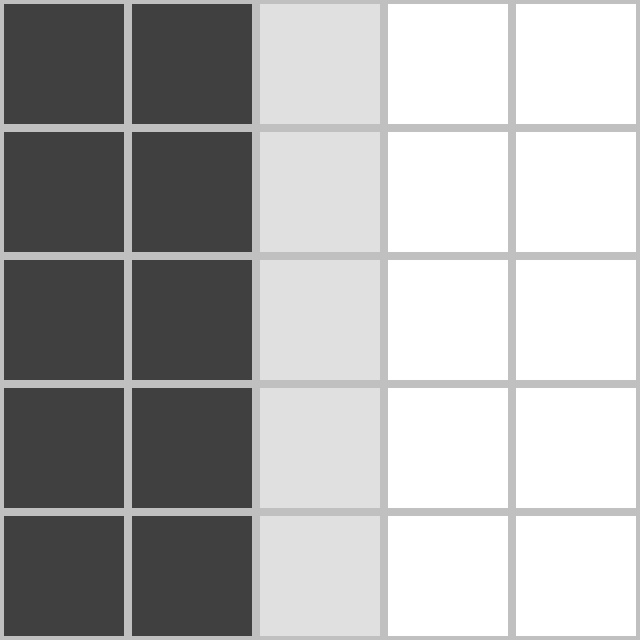
\includegraphics[width=5cm]{oscillators/phoenix_proof_1.png}};
			
			\letternode{2}{4}{A}
			\letternode{2}{3}{B}
			\letternode{2}{2}{C}
			\letternode{3}{4}{J}
			\letternode{3}{3}{K}
			\letternode{3}{2}{L}
			\letternode{4}{3}{X}
			\end{tikzpicture}}
		\caption{A diagram illustrating the fact that no phoenix can extend outside of its original bounding box (depicted by the dark grey cells) by more than one cell (depicted by the light grey cells). In particular, if the phoenix is initially confined to the dark grey cells, then cell~X can never be born.}\label{fig:phoenix_proof_1}
	\end{figure}
	
	Suppose for a contradiction that some cell at a distance of~2 from the original bounding box is eventually born, and let X be the first such cell, which is born for the first time in generation~$n$. Then cells~J, K, and L in Figure~\ref{fig:phoenix_proof_1} must each have been alive in generation~$n-1$, and since the pattern is a phoenix, they must each have been dead in generation~$n-2$. However, for cell~K to be born in generation~$n-1$, each of cells~A, B, and C must have been alive in generation~$n-2$, and thus must be dead in generation~$n-1$. We have thus shown that in generation~$n-1$, cell~K is alive and has exactly two live neighbors (J and L) and thus lives on to generation~$n$, so the pattern is not actually a phoenix.
	
	The fact that every phoenix eventually evolves into an oscillator follows immediately: there are $2^{wh}$ different patterns that fit inside a $w \times h$ box, so any pattern that stays confined to such a box forever must return to a previous phase (and thus oscillate) after no more than $2^{wh}$ generations.
\end{proof}

Before proceeding, we note that the technique used in the proof of Theorem~\ref{thm:phoenix_oscillate} is actually a very common one: to prove that a pattern with a certain property does not exist, consider what happens to the pattern at one of its far edges. We will use this same general method to prove another theorem about phoenices momentarily, and we will use it again in Section~\ref{sec:speed_limits} to find bounds on how fast spaceships can travel.

Now that we know that all phoenices evolve into oscillators, we are left with the question of what periods they can have. We already saw an example of a period~2 phoenix, but to date no one has found any phoenices with period~3 or higher. The following theorem\footnote{This theorem was also originally proved by Stephen Silver in January 2000.} shows that no phoenix of period~3 exists.

\begin{theorem}[No Phoenices with Period 3]\label{thm:phoenix_p3}
	In Conway's Game of Life, there does not exist a phoenix oscillator with period~3.
\end{theorem}

\begin{proof}
	Suppose there were a phoenix with period~3. Consider the uppermost row in the rotor of the phoenix, and let A be the leftmost cell in that row that is in the rotor, as in Figure~\ref{fig:phoenix_proof_2}. Without loss of generality, suppose that cell~A is alive in generation~3.
	
	\begin{figure}[!htb]
		\centering\gridbox{1.5pt}{\begin{tikzpicture}[scale=0.6, every node/.style={transform shape}]%
			\node[inner sep=0pt,anchor=south west] (glider_loop) at (0.5,0.5) {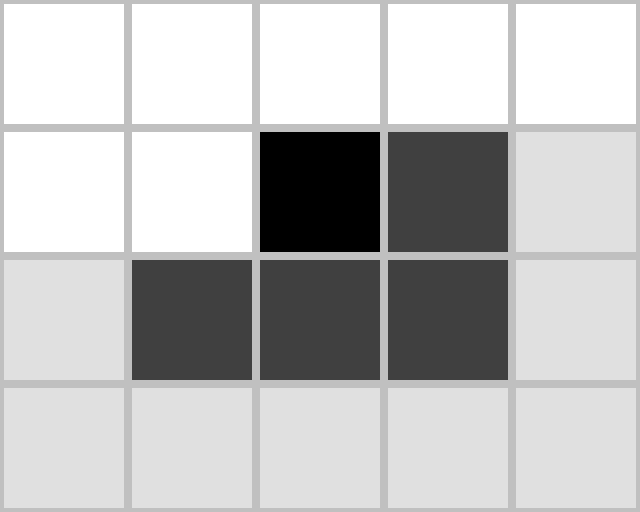
\includegraphics[width=5cm]{oscillators/phoenix_proof_2.png}};
			
			\letternode{3}{3}{A}
			\letternode{2}{2}{J}
			\letternode{3}{2}{K}
			\letternode{4}{3}{L}
			\letternode{4}{2}{M}
			\end{tikzpicture}}
		\caption{A diagram depicting the top-left corner of a hypothetical period~3 phoenix oscillator. Cell~A is the leftmost cell in the uppermost row of the oscillator, and exactly three of J, K, L, or M must be alive in the generation before A is alive.}\label{fig:phoenix_proof_2}
	\end{figure}
	
	We know that cell~A must have three neighbors that are alive in generation~2, and they must be three of the cells J, K, L, or M in Figure~\ref{fig:phoenix_proof_2}. Suppose (for a contradiction) that cell~K is alive in generation~2. Since K has at least two live neighbors in generation~2 (at least two of J, L, or M), it must in fact have at least four live neighbors (in order for it to die in generation~3). It follows that we can list K's (alive and dead) neighbors as follows:
	
	\begin{itemize}
		\item one cell (to its top-left) that is never alive,
		
		\item cell~A, which is alive in generation~3,
		
		\item at least four neighbors that are alive in generation~2, and
		
		\item exactly three neighbors (its parents) that are alive in generation~1.
	\end{itemize}
	
	Since none of the neighbors that are alive in generations~1, 2, or 3 can be the same (since it is a period~3 phoenix), we have shown that K has at least nine neighbors, which is a contradiction that shows that K must in fact be dead in generation~2. It follows that each of J, L, and M are alive in generation~2.
	\begin{figure}[!ht]
		\centering\gridbox{1.5pt}{\begin{tikzpicture}[scale=0.6, every node/.style={transform shape}]%
			\node[inner sep=0pt,anchor=south west] (glider_loop) at (0.5,0.5) {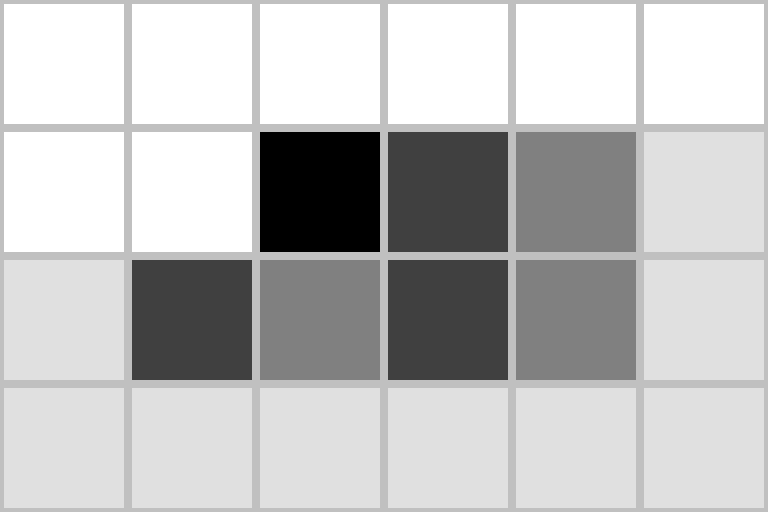
\includegraphics[width=6cm]{oscillators/phoenix_proof_3.png}};
			
			\letternode{3}{3}{A}
			\letternode{2}{2}{J}
			\letternode{3}{2}{K}
			\letternode{4}{3}{L}
			\letternode{4}{2}{M}
			\letternode{5}{3}{X}
			\letternode{5}{2}{Y}
			\end{tikzpicture}}
		\caption{A diagram that shows that no period~3 phoenix oscillator exists. Cell~A is alive in generation~3, cells J, L, and M are alive in generation~2, and cells K, X, and Y are alive in generation~1. Cell~X has only two neighbors (to its right and lower-right) that could potentially be alive in generation~0, so there was in fact no way for it to be born.}\label{fig:phoenix_proof_3}
	\end{figure}
	
	Since L must have three parents that are alive in generation~1, they must be cells K, X, and Y in Figure~\ref{fig:phoenix_proof_3}. However, there is then only room for cell~X to have at most two parents that are alive in generation~0 (in particular, the cell to its right and the cell to its lower-right), so it can't be born in generation~1, which is the contradiction that shows that this period~3 phoenix does not actually exist.
\end{proof}

A computer-assisted proof has also been used to show that no phoenices of period~5 exist,\footnote{This proof was completed by Alex Greason in September 2019.} but essentially nothing else is known about the (non-)existence of phoenices with period~4 or greater. On the other hand, if we relax the restriction on phoenices a bit and instead ask whether or not there exist higher-period oscillators with the property that every cell in the oscillator actually oscillates (i.e., the oscillator has no stator), it turns out that the answer is yes. For example, every cell in the period~3 oscillator displayed in Figure~\ref{fig:period_3_volatile} oscillates, even though it is not a phoenix.

\begin{figure}[!htb]
	\centering
	\patternimglink{0.1}{period_3_volatile}
	\caption{A period~3 oscillator with the property that every cell oscillates. Found by Jason Summers in August 2012.}\label{fig:period_3_volatile}
\end{figure}


%%%%%%%%%%%%%%%%%%%%%%%%%%%%%%%%
\section{Notes and Historical Remarks}\label{sec:oscillators_notes}
%%%%%%%%%%%%%%%%%%%%%%%%%%%%%%%%

The search for new oscillators has been one of the most consistently active research areas throughout the history of Life. Much of its motivation comes from the omniperiodicity problem---it's remarkable that such a seemingly simple problem still remains unsolved after all these years, despite the various techniques that have been developed for constructing oscillators. To illustrate just how incomplete our methods of constructing and searching for oscillators are, consider the small period~$16$ oscillators displayed in Figures~\ref{fig:rich_p16} and~\ref{fig:rob_p16}. Despite their simplicity and small size, they were not discovered until July 2016 and February 2020, respectively, and they were found in possibly the least enlightening way possible---as a result of evolving computer-generated random soups (by apgsearch\index{apgsearch}).

\begin{figure}[!htb]
	\centering
	\begin{minipage}[b]{.48\textwidth}
		\centering
		\patternimglink{0.1}{rich_p16}
		\caption{\textbf{Rich's p16}\index{Rich's p16} is a period~16 oscillator that was found in a random soup by Rich Holmes in July 2016.}\label{fig:rich_p16}
	\end{minipage} \hfill %
	\begin{minipage}[b]{.48\textwidth}
		\centering
		\patternimglink{0.114201183432}{rob_p16}
		\caption{\textbf{Rob's p16}\index{Rob's p16} is a period~16 oscillator that was found in a random soup by Rob Liston in February 2020.}\label{fig:rob_p16}
	\end{minipage}
\end{figure}

No matter how they were discovered, oscillators can be highly useful in pattern engineering, since sparkers in particular can be used for a great many purposes. We already saw that they can be used to create higher-period oscillators with composite periods, but they also form the basic building blocks of many of the large patterns that we will construct in later chapters. For example, the entirety of Chapter~\ref{chp:periodic_circuitry} is devoted to using oscillators to emulate logic circuits that can perform computations.

Many of the small billiard table oscillators that are known were found by David Buckingham, who discovered dozens of them throughout the 1970s and 1980s. Herschel tracks were also primarily his invention---he spent several years cataloguing patterns that moved B-heptominoes and Herschels from one place to another, and by October 1996 he had a complete toolkit capable of constructing oscillators and gliders guns with any period at least $61$.

Almost immediately, Paul Callahan used Herschel tracks to construct the first explicit stable glider reflector~\cite{BC98},\footnote{Although it had been known since the early 1970s that stable reflectors must exist in Life \cite{Wain74,BCG82}, no specific examples had been found prior to Callahan's construction.} which had a repeat time of $4{\thousep}840$ generations. It didn't take long for him to make some optimizations, resulting in a stable reflector with repeat time of 894 generations. Various optimizations were then made with the help of Dean Hickerson, getting the repeat time down to 747 in November 1996, followed by David Buckingham reducing the repeat time to 672 in May 1997, Stephen Silver reducing it to 623 in October 1997, Paul Callahan reducing it to 575 in November 1998, and finally Stephen Silver reducing it to 497 (as in the Silver reflector of Figure~\ref{fig:silver_reflector}) a few days later.

\begin{figure}[!htb]
	\centering\patternimglink{0.12}{period_56_herschel}
	\caption{A period~56 oscillator that was constructed using periodic Herschel conduits. It was built by Dietrich Leithner in December 1997.}\label{fig:period_56_herschel}
\end{figure}

A 180-degree stable reflector with repeat time of 202~generations, called the \textbf{boojum reflector},\footnote{In Lewis Carroll's epic poem \emph{The Hunting of the Snark}, a ``Boojum'' is a particularly dangerous type of Snark.} was found by Dave Greene in April 2001, and a 180-degree stable reflector with repeat time of 106~generations, called the \textbf{rectifier}\index{rectifier}, was found by Adam P. Goucher in March 2009 (see Exercise~\ref{exer:new_reflectors}). Finally, the Snark that we saw in Figure~\ref{fig:snark}, with a repeat time of just 43~generations, was found by Mike Playle in April 2013.

Although Buckingham's original Herschel conduits were used to construct oscillators with period~61 or higher, faster-recovering conduits can be used to create oscillators with period 58, 59, and 60 as well (see Exercise~\ref{exer:herschel_track_L112}). In December 1997, Dietrich Leithner found fast oscillating Herschel conduits that even allow for the construction of oscillators with period~56 and~57 (see Figure~\ref{fig:period_56_herschel} and Exercises~\ref{exer:period_57_herschel} and~\ref{exer:period_56_herschel}). In fact, these oscillating conduits were used to construct the first known period~57 oscillator. % http://www.radicaleye.com/lifepage/patterns/p57/p57.html

Herschel tracks remain one of the pinnacles of Life technology to this day, although they have evolved somewhat---many objects other than Herschels and B-heptominoes can be moved around tracks and converted into each other. We will return to this topic and investigate it more thoroughly in Chapter~\ref{chp:stationary_circuitry}.


\filbreak


%%%%%%%%%%%%%%%%%%%%%%%%%%%%%%%%%
\section*{Exercises \hfill \normalfont\textsf{\small solutions to starred exercises on \hyperlink{solutions_oscillators}{page \pageref{solutions_oscillators}}}}
\label{sec:oscillators_exercises}
\addcontentsline{toc}{section}{Exercises}
\vspace*{-0.4cm}\hrulefill\vspace*{-0.3cm}\footnotesize\begin{multicols}{2}\vspace*{-0.4cm}\raggedcolumns\interlinepenalty=10000
	\setlength{\parskip}{0pt}\ifdefined\FORPRINTING\colorlet{ocre}{black}\else%
\fi
	%%%%%%%%%%%%%%%%%%%%%%%%%%%%%%%%%
	
	\begin{problemstar}\label{exer:billiard_tables} \probdiff{2}
		For each of the following boxes, use induction coils to crowd the red cells and then find something that you can put in the green cells so as to make a billiard table oscillator.\vspace*{-0.25cm}
		
		\begin{multicols}{2}
			\begin{enumerate}
				\item[\bf\color{ocre}(a)] \raisebox{-\height+0.5em}{\patternimg{0.1}{exercise_billiard_table_3x3}}
				
				\item[\bf\color{ocre}(c)] \raisebox{-\height+0.5em}{\patternimg{0.1}{exercise_billiard_table_4x4}}
				
				\item[\bf\color{ocre}(b)] \raisebox{-\height+0.5em}{\patternimg{0.1}{exercise_billiard_table_skew}}
			\end{enumerate}
		\end{multicols}
	\end{problemstar}
	
	
	\mfilbreak
	
	
	\begin{problem}\label{exer:billiard_table_5x3} \probdiff{3}
		Consider the $5 \times 3$ box displayed below as a potential starting point for constructing a billiard table oscillator.
		
		\begin{center}
			\patternimglink{0.1}{billiard_table_5x3}
		\end{center}
		
		\begin{enumerate}[label=\bf\color{ocre}(\alph*)]
			\item Find a stable way to crowd the red cells, just like we used two blocks and two snakes to crowd the outside of a $4 \times 3$ box in Section~\ref{sec:billiard_tables}.
			
			\item Show that there is no way to fill in the green cells so as to make this pattern an oscillator (try writing a computer program to help you).
		\end{enumerate}
	\end{problem}
	
	
	\mfilbreak
	
	
	\begin{problem}\label{exer:eater_1_replace_eater_2_osc} \probdiff{2}
		Replace the eater~1s with eater~2s in the oscillators from the following figures, without destroying the oscillator or altering its period:\smallskip
		
		\begin{enumerate}[label=\bf\color{ocre}(\alph*)]
			\item Figure~\ref{fig:roteightor},
			
			\item Figure~\ref{fig:period_22},
			
			\item Figure~\ref{fig:worker_bee},
			
			\item Figure~\ref{fig:period_52}, and
			
			\item Figure~\ref{fig:honey_thieves} (you can only replace two of the eater~1s). 
		\end{enumerate}
	\end{problem}
	
	
	\mfilbreak
	
	
	\begin{problem}\label{exer:extend_snacker} \probdiff{1}
		The period~$9$ snacker\index{snacker} oscillator from Figure~\ref{fig:snacker} can be stabilized on one side in ways other than using two eater~1s. Use the method shown below to extend this oscillator to one that makes use of at least 5 interacting pentadecathlons.
		
		\begin{center}
			\patternimglink{0.1}{exercise_extend_snacker}
		\end{center}
	\end{problem}
	
	
	\mfilbreak
	
	
	\begin{problemstar}\label{exer:t_sparkers}\index{T-nosed p4}\index{T-nosed p6} \probdiff{2}
		Use the sparks from either the T-nosed~p$4$ or the T-nosed~p$6$ (displayed below) and another oscillator of your choice to create non-trivial oscillators with...
		
		\begin{center}
			\patternimglink{0.1}{t_nosed_p6}
		\end{center}
		
		\begin{enumerate}[label=\bf\color{ocre}(\alph*)]
			\item period~$12$,
			
			\item period~$20$, and
			
			\item period~$24$.
		\end{enumerate}
	\end{problemstar}
	
	
	\mfilbreak
	
	
	\begin{problem}\label{exer:pipsquirter_reflectors}
		One of the primary uses of pipsquirters\index{pipsquirter} is their ability to reflect a glider when a boat, block, and eater~1 are placed nearby as shown below.
		
		\begin{center}
			\patternimglink{0.1}{pipsquirter_reflector}
		\end{center}
		
		\noindent The reflector above has period~$6$. Use this same reaction to create a glider reflector with...\smallskip
		
		\begin{enumerate}[label=\bf\color{ocre}(\alph*)]
			\item \probdiff{2} period~$7$, and
			
			\item \probdiff{3} period~$8$.
		\end{enumerate}
	\end{problem}


	\mfilbreak
	
	
	\begin{problemstar}\label{exer:p32_pi_hassler_eaters} \probdiff{1}
		Show how the snakes can be replaced by eater~1s in the period~$32$ ``gourmet''\index{gourmet} oscillator from Figure~\ref{fig:p32_pi_hassler}.
	\end{problemstar}
	
	
	\mfilbreak
	
	
	\begin{problem}\label{exer:volcanoes}
		Several period~$4$ and~$5$ lightweight, middleweight, and heavyweight supervolcanoes\index{supervolcano}\index{lightweight!supervolcano}\index{middleweight!supervolcano}\index{heavyweight!supervolcano} are displayed below,\footnote{The p$4$ LW supervolcano was found by Noam Elkies in 2010, the p$5$ MW supervolcano was found by Dongook Lee in 2019, the p$5$ HW supervolcano was found by Karel Suhajda in 2004, and the rest were found by Matthias Merzenich in 2010.} and they are particularly useful due to how far they push away their sparks.
		
		\begin{center}
			\patternimglink{0.07}{supervolcanoes}
		\end{center}
		
		\begin{enumerate}[label=\bf\color{ocre}(\alph*)]
			\item \probdiff{2} Use the sparks from two supervolcanoes to construct a period~$20$ oscillator.
			
			\item \probdiff{2} Use a supervolcano and a thumb sparker to create a non-trivial period~$20$ oscillator.
			
			\item \probdiff{3} Use a supervolcano to help you construct a T-tetromino shuttle.
		\end{enumerate}
	\end{problem}
	
	
	\mfilbreak
	
	
	\begin{problemstar}\label{exer:pi_hassle} \probdiff{4}
		A domino spark can be used to rotate a pi-heptomino\index{pi-heptomino} by 90 degrees in $8$~generations, as shown below. Use this reaction to create a period~$32$ oscillator. [Hint: The spark from a figure eight does not quite work. Try some other domino sparkers---you may need to weld them together in order to make them fit together closely enough.]
		\begin{center}
			\patternlink{exercise_pi_hassle}{\vcenteredhbox{\patternimg{0.1}{exercise_pi_hassle_0}} \vcenteredhbox{\genarrow{2}} \vcenteredhbox{\patternimg{0.1}{exercise_pi_hassle_2}} \vcenteredhbox{\genarrow{6}} \vcenteredhbox{\patternimg{0.1}{exercise_pi_hassle_8}}}
		\end{center}
	\end{problemstar}
	
	
	\mfilbreak
	
	
	\begin{problemstar}\label{exer:high_period_sparkers} \probdiff{2}
		This exercise introduces some sparkers with higher period than we saw in Section~\ref{sec:sparkers}. For each of them, determine their period, find an accessible spark that they emit (the spark might only be present in one of its phases not displayed below), and use that spark to construct a non-trivial oscillator with higher period.
		\begin{multicols}{2}
			\begin{enumerate}
				\item[\bf\color{ocre}(a)] \raisebox{-\height+0.5em}{\patternimglink{0.1}{exercise_high_period_sparker_13}}
				
				\item[\bf\color{ocre}(c)] \raisebox{-\height+0.5em}{\patternimglink{0.1}{exercise_high_period_sparker_32}}
				
				\item[\bf\color{ocre}(b)] \raisebox{-\height+0.5em}{\patternimglink{0.1}{exercise_high_period_sparker_31}}
			\end{enumerate}
		\end{multicols}
	\end{problemstar}
	
	
	\mfilbreak
	
	
	\begin{problem}\label{exer:b_heptomino_hassle} \probdiff{2}
		A dot spark and an eater~2 can be used to reflect a B-heptomino\index{B-heptomino} in $11$~generations, as shown below. Use this reaction to create a period~$22$ oscillator.
		\begin{center}
			\patternlink{b_heptomino_hassle}{\vcenteredhbox{\patternimg{0.1}{b_heptomino_hassle_0}} \vcenteredhbox{\genarrow{5}} \vcenteredhbox{\patternimg{0.1}{b_heptomino_hassle_5}} \vcenteredhbox{\genarrow{6}} \vcenteredhbox{\patternimg{0.1}{b_heptomino_hassle_11}}}
		\end{center}
	\end{problem}
	
	
	\mfilbreak
	
	
	\begin{problem}\label{exer:pond_block_hasslers} \probdiff{3}
		Use the hassling reaction from Figure~\ref{fig:p27_hassler} to create an oscillator with...\smallskip
		
		\begin{enumerate}[label=\bf\color{ocre}(\alph*)]
			\item period~$24$, and% blocker works
			
			\item period~$21$, using the following p$7$ duoplet sparker:
			
			\begin{center}
				\patternimglink{0.1}{p7_duoplet_sparker}
			\end{center}
		\end{enumerate}
	\end{problem}
	
	
	\mfilbreak
	
	
	\begin{problemstar}\label{exer:p44_pi_hassler} \probdiff{3}
		A partial pi-heptomino hassler is displayed below. Complete it by placing sparkers so that domino sparks are present at the indicated locations $33$~generations after the phase shown here.
		
		\begin{center}
			\patternimglink{0.1}{exercise_pi_heptomino_hassler}
		\end{center}
		
		\noindent [Hint: What will the period of this oscillator be? Make sure that the hassler you pick has a compatible period.]
	\end{problemstar}
	
	
	\mfilbreak
	
	
	\begin{problem}\label{exer:pentadecathlon_relay_180} \probdiff{2}
		Use two pentadecathlons to construct a glider loop oscillator with period 180.
	\end{problem}
	
	
	\mfilbreak
	
	
	\begin{problem}\label{exer:snark_relay_180} \probdiff{2}
		Use four Snarks to construct an oscillator with period 180.
	\end{problem}
	
	
	\mfilbreak
	
	
	\begin{problemstar}\label{exer:six_snark_relay} \probdiff{2}
		Create a glider loop (of any period) that makes use of exactly six Snarks.
	\end{problemstar}
	
	
	\mfilbreak
	
	
	\begin{problemstar}\label{exer:snark_weld} \probdiff{3}
		Sometimes it is useful to weld together reflectors, just like we welded together eaters in the previous chapter.\smallskip
		
		\begin{enumerate}[label=\bf\color{ocre}(\alph*)]
			\item Weld together the following two partial Snarks (modify only the light gray cells), thus creating a single still life that can reflect gliders from two different sides.
			\begin{center}
				\patternimglink{0.1}{exercise_fused_snarks}
			\end{center}
			
			\item Modify the reflector from part~(a) to create a single reflector that can reflect gliders coming from four different sides.
		\end{enumerate}
	\end{problemstar}
	
	
	\mfilbreak
	
	
	\begin{problemstar}\label{exer:snark_creates_honeyfarm} \probdiff{2}
		The Snark\index{Snark} reflector works by converting the input glider into another object that we have seen before, and then converting that object into the output glider. What is the name of the intermediate object?
	\end{problemstar}
	
	
	\mfilbreak
	
	
	\begin{problemstar}\label{exer:almost_snark} \probdiff{2}
		The pattern displayed below\footnote{Found by Tanner Jacobi in 2015.} might be called an ``almost Snark'', since it can \emph{almost} be used as a $90$-degree glider reflector. Describe what goes wrong and why it cannot reflect more than one glider.
		
		\begin{center}
			\patternimglink{0.1}{almost_snark}
		\end{center}
	\end{problemstar}
	
	
	\mfilbreak
	
	
	\begin{problem}\label{exer:buckaroo_loop} \probdiff{3}
		Create a glider loop that uses at least one buckaroo and at least one twin bees shuttle. What is the smallest possible period of such an oscillator? %SOLUTION: lcm(30,46) = 690
	\end{problem}
	
	
	\mfilbreak
	
	
	\begin{problem}\label{exer:new_reflectors} \probdiff{3}
		For each of the following 180-degree stable reflectors, construct an oscillator that works by using two copies of the reflector to bounce a glider back and forth, and determine what the possible periods of such oscillators are.\smallskip
		
		\begin{enumerate}[label=\bf\color{ocre}(\alph*)]
			\item \textbf{Boojum reflector}:\index{boojum reflector} \\ \raisebox{-\height+0.5em}{\patternimg{0.1}{boojum_reflector}}\\[0.5em]
			
			\item \textbf{Rectifier}:\index{rectifier} \\ \raisebox{-\height+0.5em}{\patternimg{0.1}{rectifier}}
		\end{enumerate}
	\end{problem}
	
	
	\mfilbreak
	
	
	\begin{problem}\label{exer:machine_gun} \probdiff{3}
		Recall the 64-generation 90-degree Herschel conduit in Figure~\ref{fig:herschel_64}.\smallskip
		
		\begin{enumerate}[label=\bf\color{ocre}(\alph*)]
			\item Use four copies of the conduit to create a gun that shoots 4 gliders every 256 generations.
			
			\item Modify the pattern from part~(a) to create a period 256 oscillator. % just add eaters on the outside
			
			\item Can you add additional Herschels to this track to make an oscillator with period~128 or~64? Either explicitly construct an example or explain the problem that arises. % No, can't do this: the gliders that the Herschels emit interfere with the previous Herschels on the track.
		\end{enumerate}
	\end{problem}
	
	
	\mfilbreak
	
	
	\begin{problemstar}\label{exer:traffic_jam} \probdiff{4}
		Two reactions that move traffic lights and T-tetrominoes are displayed below (the top one is called a \textbf{traffic jam}\index{traffic jam}):
		
		\noindent\begin{center}
			\patternlink{traffic_jam}{\vcenteredhbox{\patternimg{0.1}{traffic_jam_0}} \vcenteredhbox{\genarrow{25}} \vcenteredhbox{\patternimg{0.1}{traffic_jam_25}}}
		\end{center}\vspace*{-0.35cm}
		
		\noindent\begin{center}
			\patternlink{t_tetromino_hassle_3}{\vcenteredhbox{\patternimg{0.1}{t_tetromino_hassle_3_0}} \vcenteredhbox{\genarrow{3}} \vcenteredhbox{\patternimg{0.1}{t_tetromino_hassle_3_3}} \vcenteredhbox{\genarrow{4}} \vcenteredhbox{\patternimg{0.1}{t_tetromino_hassle_3_7}} \vcenteredhbox{\genarrow{4}} \vcenteredhbox{\patternimg{0.1}{t_tetromino_hassle_3_11}}}
		\end{center}
		
		\noindent Use these reactions (and optionally any of the other T-tetromino hassling reactions we have seen) to create an oscillator.
	\end{problemstar}
	
	
	\mfilbreak
	
	
	\begin{problemstar}\label{exer:traffic_jam_reflect} \probdiff{3}
		What type of sparks does the traffic jam reaction from the top of Exercise~\ref{exer:traffic_jam} produce? Use this spark and the oscillator constructed in Exercise~\ref{exer:traffic_jam} to create a periodic glider reflector.
	\end{problemstar}
	
	
	\mfilbreak
	
	
	\begin{problem}\label{exer:herschel_track_1} \probdiff{3}
		Use the R64 and Fx77 conduits to construct Herschel track oscillators or guns with the following periods.
		
		\noindent [Hint: Mimic our construction in Figure~\ref{fig:herschel_track_oscillators}.]\smallskip
		
		\begin{enumerate}[label=\bf\color{ocre}(\alph*)]
			\item Period~$218$ oscillator.
			
			\item Period~$62$ oscillator.
			
			\item Period~$69$ glider gun.
			
			\item Period~$61$ oscillator.
			
			\item Period~$70$ glider gun.
		\end{enumerate}
	\end{problem}
	
	
	\mfilbreak
	
	
	\begin{problem}\label{exer:herschel_track_2_what_periods} \probdiff{2}
		By placing different numbers of Herschels on the track from Figure~\ref{fig:herschel_track_2}, oscillators of which periods can be created?
	\end{problem}
	
	
	\mfilbreak
	
	
	\begin{problem}\label{exer:herschel_track_L112}
		Consider the Herschel conduit displayed below, which rotates a Herschel counter-clockwise in 112 generations and has a repeat time of 58 generations. This conduit is called \textbf{L112}\index{L112}.
		
		\begin{center}
			\patternimglink{0.1}{L112}
		\end{center}
		
		\begin{enumerate}[label=\bf\color{ocre}(\alph*)]
			\item \probdiff{3} Construct a period~109 oscillator by using only the L112 and Fx77 conduits (and possibly some eaters to destroy stray gliders).
			
			\item \probdiff{4} The L112 conduit has a slightly faster repeat time than the R64 conduit (58 generations instead of 61). Use the L112 and Fx77 conduits to create an oscillator with period~58, 59, or 60. [Hint: Refer back to the footnote in Section~\ref{sec:herschel_track} about the Fx77 conduit's repeat time.]
		\end{enumerate}
	\end{problem}


	\mfilbreak
	
	
	\begin{problemstar}\label{exer:phoenix_bb} \probdiff{3}
		Based on the phoenix oscillator shown in Figure~\ref{fig:phoenix}, we might be tempted to guess that Theorem~\ref{thm:phoenix_oscillate} can be improved to show that no phoenix can ever leave its original bounding box at all. Show that this conjecture is false. That is, find a phoenix that does in fact leave its original bounding box.
	\end{problemstar}
	
	
	\mfilbreak
	
	
	\begin{problem}\label{exer:period_57_herschel} \probdiff{4}
		Consider the (oscillating!) Herschel conduit displayed below, which rotates a Herschel counter-clockwise and flips it in 65 generations, and has a repeat time of 57 generations. Construct a period~57 oscillator by using this new conduit and the Fx77 conduit (and possibly some eaters to destroy stray gliders).
		\begin{center}
			\patternimglink{0.1}{period_57_herschel}
		\end{center}
	\end{problem}
	
	
	\mfilbreak
	
	
	\begin{problem}\label{exer:period_56_herschel} \probdiff{3}
		Consider the period~56 Herschel track oscillator depicted in Figure~\ref{fig:period_56_herschel}. Break this oscillator down into its individual conduits, and for each conduit state (a) how many generations it takes a Herschel to traverse the conduit, and (b) what the conduit's repeat time is. Also break down each conduit into still lifes, oscillators, and eaters that we have seen earlier.
	\end{problem}
	
	
	\mfilbreak
	
	
	\begin{problemstar}\label{exer:p4_oscillator} \probdiff{4}
		Prove that there is no period~4 oscillator with exactly one cell that oscillates at the full period.
	\end{problemstar}


	\mfilbreak
	
	
	\begin{problem}\label{exer:p4_oscillator_impb} \probdiff{4}
		Prove that there is no period~4 oscillator whose rotor consists of exactly $4$ cells, which take turns being alive for one generation out of each four.
	\end{problem}
% SOLUTION (from Dean Hickerson): If you mean that there are only 4 active cells, A, B, C, and D, such that exactly one is alive in each phase, then there's no such object. For suppose that A is alive in gen 0 and B is alive in gen 1. Then B must be born in gen 1, so it has either 2 or 3 neighbors among the stable cells (2 if B is adjacent to A, 3 otherwise). But then B must survive into gen 2, a contradiction.
	
	
	\mfilbreak
	
	
	\begin{problemstar}\label{exer:period_3_volatile} \probdiff{2}
		The period~3 oscillator presented in Figure~\ref{fig:period_3_volatile} was constructed by putting together the various period~3 ``pieces'' displayed below. Use these same pieces to construct a larger period~3 oscillator with at least 200 live cells in one of its phases.
		\begin{center}
			\patternimglink{0.085}{period_3_volatile_pieces}
		\end{center}
	\end{problemstar}
	
	%% EXERCISE END COMMANDS
\end{multicols}
\normalsize\vspace*{0.01cm}\ifdefined\FORPRINTING\colorlet{ocre}{rawocre}\else%
\fi
%% DONE EXERCISE END COMMANDS


%%%%%%%%%%%%%%%%%%%%%%%%%%%%%%%%%%%%%%%%%%%%%%%%%%%%%%%%%%%%%%%%%%%%%%%%%
%%   CHAPTER: SPACESHIPS AND MOVING OBJECTS
%%%%%%%%%%%%%%%%%%%%%%%%%%%%%%%%%%%%%%%%%%%%%%%%%%%%%%%%%%%%%%%%%%%%%%%%%

\renewcommand{\chapterfolder}{spaceships/}
\chapterimage{cover/spaceships}
\chapter{Spaceships and Moving Objects}\label{chp:spaceships}


\vspace*{-0.4in}
\epigraph{Life is like riding a bicycle; to keep your balance, you must keep moving.}{Albert Einstein}
\vspace*{0.4in}


\noindent We now shift our focus from stationary objects, like still lifes and oscillators, to moving objects, like spaceships\index{spaceship} and puffers. Recall that a spaceship is a pattern that returns to its initial phase after $2$ or more generations, but at a different location from where it started. Just as was the case for oscillators, the \textbf{period}\index{period} of a spaceship is the smallest number of generations needed for it to return to its initial phase.

We can also talk about the \textbf{speed}\index{speed} of moving objects: the number of cells that they move on average per generation. Since no object in the Life plane could possibly move at a speed of greater than $1$ cell (in the Moore neighborhood sense) per generation, this speed is typically referred to as the \textbf{speed of light}\index{speed of light} and is denoted by $c$, while other speeds are represented as fractions of $c$. For example, since the glider moves diagonally by $1$ cell every $4$ generations, on average it moves $1/4$ cell per generation, so it has a speed of $c/4$. Similarly, the light/middle/heavyweight spaceships move $2$ cells every $4$ generations, and thus have a speed of $2c/4 = c/2$ (see Figure~\ref{fig:basic_spaceships}).

\begin{figure}[!htb]
	\centering
	\patternimglink{0.1}{basic_spaceships}
	\caption{The four basic spaceships in Conway's Game of Life. From left to right, these are the glider (which moves diagonally at a speed of $c/4$) and the light/middle/heavyweight spaceships (which each move orthogonally\protect\footnotemark \ at a speed of $c/2$).}\label{fig:basic_spaceships}
\end{figure}

\footnotetext{The term \textbf{orthogonal} means straight left--right or up--down, as opposed to diagonal.}Although some of the first objects that we ever encountered in Life were spaceships, constructing new ones is actually quite a difficult problem, and a far smaller variety of spaceships is known than of still lifes or oscillators. In fact, finding new spaceships is so difficult that the four ``basic'' types of spaceships, together with some of their tagalongs (which we will introduce shortly), were the only known spaceships for the first 19 years of Life's history.\footnote{Dean Hickerson found the first known truly new spaceships via computer search in 1989.} Due to the difficulty of constructing new spaceships, instead of focusing on methods of construction, much of this chapter will focus on investigating what we can \emph{do} with the spaceships that we already have.



\section{The Glider}\label{sec:glider}

The glider is the single most useful spaceship that exists,\footnote{And arguably the single most useful \emph{pattern} that exists.} since its small size and frequent appearance from random soups make it easy to generate and manipulate. We have already seen numerous methods of generating gliders: the Gosper glider gun\index{Gosper glider gun} of Section~\ref{sec:queen_bee}, the twin bees gun\index{twin bees!gun} of Section~\ref{sec:twin_bees}, and the glider-producing switch engine of Section~\ref{sec:switch_engine}. We will not present any additional methods of constructing gliders here, but we will see some as we progress through the book, including some moving sources of gliders in Section~\ref{sec:rakes}, and glider guns of any period of our choosing in Chapter~\ref{chp:guns}.

We have also seen that we can delete gliders (Section~\ref{sec:eaters}) and that we can reflect gliders (Section~\ref{sec:glider_loops}). When we start manipulating gliders via these types of patterns, it will be important for us to be able to talk about the relative timings and positions of different gliders, so we now introduce some terminology that lets use do so.


\subsection{Color of a Glider}\label{sec:glider_color}\index{glider!color}

When reflecting a glider\index{reflector}, it is important to be aware of the glider's \textbf{color},\footnote{The term \textbf{parity} is sometimes used instead of color.} which is a property of a glider that stays constant as it moves, but can change when it hits a reflector. Specifically, imagine that the Life grid is colored with two colors like a checkerboard, with adjacent cells (in the von Neumann neighborhood sense) always having different colors. The color of a glider is the color of its leading cell when it is in the phase that can be rotated to look like the glider in Figure~\ref{fig:glider_color_1}.

It is worth emphasizing two potential points of confusion regarding glider color:\medskip

\begin{itemize}
	\item The color of a glider's leading cell in its phases \emph{other} than the one from Figure~\ref{fig:glider_color_1} is irrelevant. For example, all of the gliders in Figure~\ref{fig:glider_color} have the same color as each other, since after evolving them into the correct phase, their leading cell is on a white cell of the checkerboard pattern.\smallskip
	
	\item We typically consider the color of a glider as a relative property, not an absolute one. That is, we talk about two gliders having the same or different color, but it is not often useful to talk about a single glider having a certain color.\medskip
\end{itemize}

\begin{figure}[!htb]
	\centering
	\begin{minipage}[b]{.3\textwidth}
		\centering\vcenteredhbox{	\centering\vcenteredhbox{\begin{tikzpicture}[scale=1.5, every node/.style={transform shape}]%
				\node[inner sep=0pt,anchor=south west] at (0,0) {\patternimg{0.1}{glider_color_1}};
				\draw[white,line width=3pt,opacity=0.6](0.61,0.275) circle (0.165);
				\draw[redback2,line width=1.25pt](0.61,0.275) circle (0.165);
				\end{tikzpicture}}}
		\caption{This glider's color is white since its leading cell (circled in \bgbox{redback}{red}) is located at one of the white cells on the checkerboard pattern.}\label{fig:glider_color_1}
	\end{minipage} \hfill %
	\begin{minipage}[b]{.66\textwidth}
		\centering
		\patternimglink{0.11}{glider_color}
		\caption{A collection of $16$ gliders that all have the same color as each other. If any of these gliders were moved to the left, right, up, or down by $1$ cell then their color would change.}\label{fig:glider_color}
	\end{minipage}
\end{figure}

To illustrate why a glider's color is important, consider the task of reflecting a glider as in Figure~\ref{fig:reflect_glider_change}. We might first try to use the Snark\index{Snark} to perform the reflection, but we quickly find that no matter how we place the Snark in the path of the input glider, the output glider never quite ends up where we want it. The reason for this is that the desired input and output gliders have opposite colors, but the Snark always produces an output glider that has the same color as its input. For this reason, the Snark is called a \textbf{color-preserving}\index{color-preserving} reflector, and we instead need a \textbf{color-changing}\index{color-changing} reflector to get the output glider to travel through the desired location. One color-changing glider reflector that we have already seen is the twin bees shuttle (recall from Figure~\ref{fig:twin_bees_shuttle_spark} how it can be used as a reflector), which can reflect the glider in the desired manner as in Figure~\ref{fig:reflect_glider_change_bees}.

\begin{figure}[!htb]
	\centering
	\begin{minipage}[b]{.41\textwidth}
		\centering
		\patternimglink{0.13}{reflect_glider_change}
		\caption{A path along which we would like to reflect a glider. Notice that the reflected glider has the opposite color of the original glider.}\label{fig:reflect_glider_change}
	\end{minipage} \hfill %
	\begin{minipage}[b]{.55\textwidth}
		\centering
		\patternimglink{0.09}{reflect_glider_change_bees}
		\caption{Twin bees shuttle is a color-changing reflector that can be used to reflect the glider in the desired way.}\label{fig:reflect_glider_change_bees}
	\end{minipage}
\end{figure}

Keeping track of a glider's color also helps us keep track of which types of glider loops are and are not possible. For example, it is not possible to construct a glider loop that uses 3~Snarks and a single twin bees shuttle, since the twin bees shuttle will change the glider's color, but it won't be changed back before hitting the twin bees shuttle again, and thus can't possibly return back to where it started. In general, every glider loop must make use of an even number of color-changing reflectors.


\subsection{Glider Lanes and Timing}\label{sec:glider_lanes}

Sometimes it is useful to compare not just the color of two gliders, but also the exact amount by which their positions differ. More specifically, we would like to be able to discuss how far gliders are in front of other gliders (even if they are somewhat offset to the side of each other), and we would also like a way of discussing how far to the side of each other they are. We can only really make these comparisons if the gliders are traveling in the same direction, so all gliders that we consider throughout this section are (arbitrarily) chosen to travel from the top-left to the bottom-right.

First, we partition the Life plane into diagonal lines of cells with slope $-1$, which we call \textbf{lanes}\index{glider!lane}. We choose one of these lanes to be ``lane $0$'' and then number the lanes so that they increase from left to right. Then we say that the lane of a glider is the lane occupied by the glider's leading cell when it is in the phase displayed in Figure~\ref{fig:glider_lanes}, much like we defined the color of a glider in terms of the location of this phase's leading cell.\footnote{In fact, a glider's color can just be thought of as its lane modulo $2$.} For brevity, we sometimes refer to a single lane separation as a \textbf{half diagonal}\index{half diagonal}\index{hd|see {half diagonal}} (or \textbf{hd} for short) and a two-lane separation as a \textbf{full diagonal}\index{full diagonal}\index{fd|see {full diagonal}} (or \textbf{fd} for short). For example, if two gliders are separated by $4$ lanes then we might say that their spacing is ``4hd'' or ``2fd''.

\begin{figure}[!htb]
	\centering
	\gridbox{0.75pt}{\begin{tikzpicture}[scale=0.55, every node/.style={transform shape}]%
		\node[inner sep=0pt,anchor=south west] (glider_loop) at (0.5,0.5) {\patternimgwidth{9cm}{glider_slope_chart}};
		
		\letternode{1}{1}{$\cdot$}
		
		\letternode{1}{2}{$\cdot$}
		\letternode{2}{1}{$\cdot$}
		
		\letternode{1}{3}{-5}
		\letternode{2}{2}{-5}
		\letternode{3}{1}{-5}
		
		\letternode{1}{4}{-4}
		\letternode{2}{3}{-4}
		\letternode{3}{2}{-4}
		\letternode{4}{1}{-4}
		
		\letternode{1}{5}{-3}
		\letternode{2}{4}{-3}
		\letternode{3}{3}{-3}
		\letternode{4}{2}{-3}
		\letternode{5}{1}{-3}
		
		\letternode{1}{6}{-2}
		\letternode{2}{5}{-2}
		\letternode{3}{4}{-2}
		%\letternode{4}{3}{-2}
		\letternode{5}{2}{-2}
		\letternode{6}{1}{-2}
		
		\letternode{1}{7}{-1}
		\letternode{2}{6}{-1}
		\letternode{3}{5}{-1}
		\letternode{4}{4}{-1}
		%\letternode{5}{3}{-1}
		\letternode{6}{2}{-1}
		\letternode{7}{1}{-1}
		
		\letternode{2}{7}{0}
		\letternode{3}{6}{0}
		\letternode{4}{5}{0}
		\letternode{5}{4}{0}
		%\letternode{6}{3}{0}
		\letternode{7}{2}{0}
		\letternode{8}{1}{0}
		
		\letternode{3}{7}{1}
		\letternode{4}{6}{1}
		%\letternode{5}{5}{1}
		%\letternode{6}{4}{1}
		\letternode{7}{3}{1}
		\letternode{8}{2}{1}
		\letternode{9}{1}{1}
		
		\letternode{4}{7}{2}
		\letternode{5}{6}{2}
		\letternode{6}{5}{2}
		\letternode{7}{4}{2}
		\letternode{8}{3}{2}
		\letternode{9}{2}{2}
		
		\letternode{5}{7}{3}
		\letternode{6}{6}{3}
		\letternode{7}{5}{3}
		\letternode{8}{4}{3}
		\letternode{9}{3}{3}
		
		\letternode{6}{7}{4}
		\letternode{7}{6}{4}
		\letternode{8}{5}{4}
		\letternode{9}{4}{4}
		
		\letternode{7}{7}{5}
		\letternode{8}{6}{5}
		\letternode{9}{5}{5}
		
		\letternode{8}{7}{$\cdot$}
		\letternode{9}{6}{$\cdot$}
		
		\letternode{9}{7}{$\cdot$}
		\end{tikzpicture}}
	\caption{A glider that is in lane~$0$, which is highlighted in light grey. The numbers on the grid indicate the lane number of each cell in the plane, and the lane of every glider in the plane is determined by the location of its leading cell when it is in the phase displayed here.}\label{fig:glider_lanes}
\end{figure}

Comparing the \textbf{timing}\index{glider!timing} of gliders is straightforward if they are in the same lane: we choose some glider in that lane to have timing $0$ when it is in the phase depicted in Figure~\ref{fig:glider_lanes}, and we say that the timing of any other glider in that lane is the number of generations needed to move the glider with timing~$0$ to its position. To extend this definition so that we can compare the timing of gliders in different lanes, we then say that gliders of the same color have the same timing as each other if they are on the same diagonal line of slope~$1$,\footnote{That is, the same diagonal that goes from bottom-left to top-right.} and we say that a glider of the opposite color has timing $2$ generations higher than a glider that is one cell to its left. These timing rules are illustrated in Figure~\ref{fig:glider_timings}.

\begin{figure}[!htb]
	\centering
	\gridbox{0.75pt}{\begin{tikzpicture}[scale=0.55, every node/.style={transform shape}]%
		\node[inner sep=0pt,anchor=south west] (glider_loop) at (0.5,0.5) {\patternimgwidth{8cm}{glider_slope_chart_b}};
		
		\letternode{1}{6}{$\cdot$}
		\letternode{2}{6}{$\cdot$}
		\letternode{1}{5}{$\cdot$}
		
		\letternode{3}{6}{-8}
		\letternode{2}{5}{-8}
		\letternode{1}{4}{-8}
		
		\letternode{5}{6}{-4}
		\letternode{4}{6}{-6}
		\letternode{4}{5}{-4}
		%\letternode{3}{5}{-6}
		\letternode{3}{4}{-4}
		\letternode{2}{4}{-6}
		%\letternode{2}{3}{-4}
		\letternode{1}{3}{-6}
		\letternode{1}{2}{-4}
		
		\letternode{7}{6}{0}
		\letternode{6}{6}{-2}
		\letternode{6}{5}{0}
		\letternode{5}{5}{-2}
		\letternode{5}{4}{0}
		%\letternode{4}{4}{-2}
		%\letternode{4}{3}{0}
		%\letternode{3}{3}{-2}
		\letternode{3}{2}{0}
		\letternode{2}{2}{-2}
		\letternode{2}{1}{0}
		\letternode{1}{1}{-2}
		
		\letternode{8}{6}{2}
		\letternode{8}{5}{4}
		\letternode{7}{5}{2}
		\letternode{7}{4}{4}
		\letternode{6}{4}{2}
		\letternode{6}{3}{4}
		\letternode{5}{3}{2}
		\letternode{5}{2}{4}
		\letternode{4}{2}{2}
		\letternode{4}{1}{4}
		\letternode{3}{1}{2}
		
		\letternode{8}{4}{6}
		\letternode{8}{3}{8}
		\letternode{7}{3}{6}
		\letternode{7}{2}{8}
		\letternode{6}{2}{6}
		\letternode{6}{1}{8}
		\letternode{5}{1}{6}
		
		\letternode{8}{2}{$\cdot$}
		\letternode{8}{1}{$\cdot$}
		\letternode{7}{1}{$\cdot$}
		
		\end{tikzpicture}}
	\caption{A glider that has timing~$0$, with the diagonal line of light grey cells indicating the other locations of leading cells that are considered to have timing~$0$. The numbers on the grid indicate the timing of a glider when its leading cell is in that location.}\label{fig:glider_timings}
\end{figure}

Just as with glider color, we are typically not interested in the absolute lane number or absolute timing of a single glider, but rather we talk about the number of lanes between two gliders and the number of generations by which their timing differs.


\subsection{Tagalongs}\label{sec:glider_tagalongs}

Some spaceships, especially ones that emit accessible sparks, are capable of carrying other objects along with them as they move. Such objects are called \textbf{tagalongs}\index{tagalong}, and we now look at some examples of objects that can tag along with the glider. Although the glider does not really have any sparks, its rearmost cell is nonetheless far enough away from the body of the glider that it can carry some tagalongs with it, as demonstrated in Figure~\ref{fig:glider_tagalongs}. Notice that these tagalongs do not actually touch the glider in any of these examples---rather, the back end of the glider only serves to overpopulate the front end of the tagalong.

\begin{figure}[!htb]
	\centering
	\begin{tabular}{@{}cccc@{}}
		\begin{subfigure}{.29\textwidth}
			\centering
			\patternimglink{0.116551724138}{b29}
			\caption{\textbf{B29}\index{B29}}
			\label{fig:b29}
		\end{subfigure} &
		\begin{subfigure}{.22\textwidth}
			\centering
			\patternimglink{0.1}{canada_goose}
			\caption{\textbf{Canada goose}\index{Canada goose}}
			\label{fig:canada_goose}
		\end{subfigure} &
		\begin{subfigure}{.21\textwidth}
			\centering
			\patternimglink{0.1}{crab}
			\caption{\textbf{crab}\index{crab}}
			\label{fig:crab}
		\end{subfigure} &
		\begin{subfigure}{.2\textwidth}
			\centering
			\patternimglink{0.093370165745}{orion_2}
			\caption{\textbf{Orion 2}\index{Orion 2}}
			\label{fig:orion_2}
		\end{subfigure}
	\end{tabular}
	\caption{Some tagalongs (highlighted in \bgbox{greenback}{green}) that can trail behind a glider. They were found by (a)~Hartmut Holzwart in 2004, and Jason Summers in (c) 2000, and (b,d) 1999.\protect\footnotemark}
	\label{fig:glider_tagalongs}
\end{figure}

\footnotetext{The name ``Orion 2'' is a reference to a similar, but larger, spaceship called \textbf{Orion}\index{Orion} that was found by Hartmut Holzwart in 1993.}One useful feature of tagalongs is that they often themselves emit sparks as well, so we can sometimes chain them together or use them to produce reactions that are impossible with the original spaceship itself. For example, the B29 tagalong emits both a dot spark and a domino spark (displayed at the top center in Figure~\ref{fig:b29}), which other tagalongs can latch onto, as in Figure~\ref{fig:b29_tagalong}. Furthermore, \emph{this} new tagalong also emits a dot spark, which allows it to pull additional tagalongs, and in this way we develop a sort of grammar for $c/4$ diagonal spaceships: there are dozens of different $c/4$ diagonal tagalongs known, and we can construct a wide variety of $c/4$ diagonal spaceships by attaching these tagalongs to each other in different ways.

Similarly, the crab emits a dot spark (seen at its back left in Figure~\ref{fig:crab}) that can be used to turn a tub\index{tub} into a barge\index{barge}, and then a long barge\index{long barge}, and then a long long barge, and so on, as illustrated in Figure~\ref{fig:tubstretcher}. A pattern with this property is called a \textbf{tubstretcher}\index{tubstretcher}, or more generally a \textbf{wickstretcher}\index{wickstretcher} if we do not care about which particular object is stretched.

\begin{figure}[!htb]
	\centering
	\begin{minipage}[b]{.37\textwidth}
		\centering
		\patternimglink{0.082614107883}{b29_tagalong}
		\caption{The B29 can pull a tagalong (highlighted in \bgbox{orangeback}{orange}) that was found by Nicolay Beluchenko in 2005.}\label{fig:b29_tagalong}
	\end{minipage} \hfill %
	\begin{minipage}[b]{.59\textwidth}
		\centering
		\embedlink{tubstretcher}{\vcenteredhbox{\patternimg{0.11}{tubstretcher_0}} \vcenteredhbox{\genarrow{4}} \vcenteredhbox{\patternimg{0.11}{tubstretcher_4}}}
		\caption{A pattern based on the crab called a \textbf{tubstretcher} that lengthens a tub (highlighted in \bgbox{orangeback}{orange}) by $2$ cells every $4$ generations.}\label{fig:tubstretcher}
	\end{minipage}
\end{figure}

While we have seen infinitely-growing patterns before (such as the Gosper glider gun\index{Gosper glider gun} in Section~\ref{sec:queen_bee} and some switch engine puffers in Section~\ref{sec:switch_engine}), it is worth observing that all infinitely-growing patterns that we saw previously worked by creating many disconnected small objects, whereas this one is quite different in that it creates a single arbitrarily-large object.



\section{The Light, Middle, and Heavyweight Spaceships}\label{sec:lwss_mwss_hwss}

Although the glider is the easiest spaceship to create and manipulate, the light, middle, and heavyweight spaceships are often better at manipulating \emph{other} objects. The reason that they can interact with so many other patterns in such a wide variety of ways is that they emit such accessible sparks so frequently. Every second generation, the LWSS emits a dot spark and a thumb spark\index{dot spark}\index{thumb spark}, the MWSS emits two dot sparks and a thumb spark, and the HWSS emits a dot spark, a domino spark\index{domino spark}, and a thumb spark (see Figure~\ref{fig:lwss_mwss_hwssb}).

\begin{figure}[!htb]
	\centering \patternimglink{0.1}{lwss_mwss_hwss}
	\caption{The light, middle, and heavyweight spaceship each give off several sparks (depicted in \bgbox{orangeback}{orange}) that are extremely useful.}\label{fig:lwss_mwss_hwssb}
\end{figure}

One useful feature of these sparks is their ability to destroy other nearby objects, as demonstrated in Figure~\ref{fig:orthogonal_destroy}. The most common use of these reactions is to adjust the debris left behind by puffers. For example, suppose that we had a $c/2$ orthogonal puffer that left behind a combination of blocks, blinkers, and gliders as it moved. By carefully positioning some middleweight spaceships behind this puffer, we could eliminate the unwanted debris (typically the blocks and blinkers), leaving only the desired output (typically the gliders).

\begin{figure}[!htb]
	\centering \patternimglink{0.1}{orthogonal_destroy}
	\caption{Light, middle, and heavyweight spaceships about to destroy some common small objects.}\label{fig:orthogonal_destroy}
\end{figure}

On the other hand, it is also often useful to have other objects destroy these spaceships. We already saw how an eater~1\index{eater!1} can destroy an LWSS or MWSS in Figure~\ref{fig:eater_1_multi}, and an eater~2\index{eater!2} can destroy an LWSS or MWSS as in Exercise~\ref{exer:eater_2_lwss_mwss}. Destroying an HWSS is slightly trickier, but three eaters that work are presented in Figure~\ref{fig:hwss_eat}. The first of these eaters has the downside of being rather large, whereas the second eater has a very high recovery time; the pond and block are completely destroyed by the HWSS, leaving behind a beehive and a glider which then collide, miraculously reconstructing the block and pond exactly in their original positions.\footnote{This reaction in which a glider turns a beehive into a pond and block is called a \textbf{honey bit}.}\index{honey!bit} The third eater is small and has a fast recovery time, but at the expense of having period~$2$ and thus only being able to destroy streams of heavyweight spaceships with even period.\footnote{The large stable HWSS eater was found by Dean Hickerson in 1999 (with a slight size improvement by Karel Suhajda in 2003), and the eater comprised of a pond and a block was found by Brice Due in 2007. The killer toads have been known since the very early days of Life.}

\begin{figure}[!htb]
	\centering \patternimglink{0.08}{hwss_eat1} \qquad \patternimglink{0.123308270677}{hwss_eat2} \qquad \patternimglink{0.123308270677}{killer_toads}
	\caption{Three methods of eating a heavyweight spaceship. The arrangement of two toads\index{toad} on the right is called \textbf{killer toads}\index{killer toads}, and it can also eat many other objects, such as an MWSS in the same position.}\label{fig:hwss_eat}
\end{figure}
% There is an LWSS eater made up of 2 blocks (ss-eaters.rle in Golly)


\subsection{Flotillae and Tagalongs}\label{sec:flotillas}\index{tagalong}

Just like we could attach various tagalongs to the back of a glider, we can also use tagalongs to extend the light, middle, and heavyweight spaceships. Some of these tagalongs are presented in Figure~\ref{fig:lwss_tagalongs}. The \textbf{hivenudger} of Figure~\ref{fig:hivenudger} (whose name comes from the fact that it pushes a pre-beehive\index{pre-beehive}) is somewhat versatile in that any of the lightweight spaceships at its corners can be replaced by a middleweight or heavyweight spaceship (see Exercise~\ref{exer:hivenudger_modify}).

\begin{figure}[!htb]
	\centering
	\begin{tabular}{@{}cccc@{}}
		\begin{subfigure}{.21\textwidth}
			\centering
			\patternimglink{0.112455621302}{sidecar}
			\caption{\textbf{Sidecar}\index{sidecar}}
			\label{fig:sidecar}
		\end{subfigure} &
		\begin{subfigure}{.22\textwidth}
			\centering
			\patternimglink{0.105}{hwss_x66}
			\caption{HWSS tagalong}
			\label{fig:hwss_x66}
		\end{subfigure} &
		\begin{subfigure}{.24\textwidth}
			\centering
			\patternimglink{0.09847150259}{pushalong}
			\caption{MWSS tagalong}
			\label{fig:pushalong}
		\end{subfigure} &
		\begin{subfigure}{.25\textwidth}
			\centering
			\patternimglink{0.092707317073}{hivenudger}
			\caption{\textbf{Hivenudger}\index{hivenudger}}
			\label{fig:hivenudger}
		\end{subfigure}
	\end{tabular}
	\caption{Some small tagalongs (highlighted in \bgbox{greenback}{green}) for light, middle, and heavyweight spaceships. These tagalongs were found in 1992 by (a,b,d) Hartmut Holzwart and (c) David Bell.}
	\label{fig:lwss_tagalongs}
\end{figure}

The MWSS tagalong in Figure~\ref{fig:pushalong} is somewhat special for the fact that it attaches to the front end of a spaceship, rather than its side or rear. Tagalongs with this property are sometimes called \textbf{pushalongs}\index{pushalong}, and they are quite a bit rarer than other types of tagalongs, since it is not common for spaceships to have accessible sparks near their front that can support another object (for example, no pushalongs for the glider are known). There are two other particularly useful tagalongs for the light, middle, and heavyweight spaceships, called the \textbf{Schick engine} and \textbf{Coe ship}. We will introduce and thoroughly investigate these tagalongs in Section~\ref{sec:rakes}.

Just like we distinguished between strict still lifes and pseudo still lifes in Section~\ref{sec:pseudo_strict_still_lifes}, we similarly distinguish between spaceships\footnote{The term ``strict spaceship'' is not used in practice, and if the term ``spaceship'' is used unqualified then it is typically assumed that it cannot be broken down into smaller spaceships.} and \textbf{pseudo spaceships}\index{pseudo!spaceship}, which are flotillae in which none of the component spaceships actually change their evolution at all, but at least one dead cell has more than $3$ live neighbours in the flotilla but has fewer than $3$ live neighbors when only one of the component spaceships is present. Some pseudo spaceships involving lightweight and heavyweight spaceships are displayed in Figure~\ref{fig:lwss_hwss_pseudo}.

\begin{figure}[!htb]
	\centering
	\patternimglink{0.1}{lwss_hwss_pseudo}
	\caption{There are three ways of placing a LWSS, MWSS, and/or HWSS next to each other so as to create a pseudo spaceship. In all three of these cases, the component spaceships evolve in the exact same way as they would individually, yet in some of their phases the flotilla overpopulates some cells (highlighted in \bgbox{redback}{red}) that the spaceships individually do not.}\label{fig:lwss_hwss_pseudo}
\end{figure}

It is also possible for the sparks of two light, middle, and heavyweight spaceships to interact with each other as they move, similar to how we used the sparks of two oscillators to interact with each other in Section~\ref{sec:composite_periods}. Objects created from multiple smaller interacting spaceships like this are called \textbf{flotillae}\index{flotilla}, and some examples involving a lightweight spaceship and a middleweight spaceship are presented in Figure~\ref{fig:lwss_mwss_flotillae}. Since flotillae can be made up of multiple copies of any of these three standard $c/2$ orthogonal spaceships--LWSS, MWSS, or HWSS--it is often convenient to refer to them as an \textbf{xWSS}.\index{xWSS} This term comes from the idea of ``x'' being an unknown, which can be replaced by one of the other letters, ``L'', ``M'', or ``H''.

Although there are numerous\footnote{To be explicit, the number of flotillae involving two xWSSes are: 1 LWSS on LWSS (pseudo), 3 LWSS on MWSS, 8 LWSS on HWSS ($1$ is pseudo), 5 MWSS on MWSS, 15 MWSS on HWSS, and 10 HWSS on HWSS ($1$ is pseudo).} ways of creating flotillae, they are a bit less satisfying than what we got when we combined oscillator sparks in Section~\ref{sec:composite_periods}. The main reason these flotillae do not really get us too much that is genuinely ``new'' is that each of the light, middle, and heavyweight spaceships have the same period and speed, so every flotilla constructed from them will also have the same period and speed.

\begin{figure}[!htb]
	\centering
	\begin{minipage}{.28\textwidth}
		\centering
		\embedlink{lwss_mwss_flotillae}{\vcenteredhbox{\patternimg{0.1}{lwss_mwss_flotillae_1_0}} \vcenteredhbox{\genarrow{1}} \vcenteredhbox{\patternimg{0.1}{lwss_mwss_flotillae_1_1}}}
	\end{minipage} \hfill %
	\begin{minipage}{.37\textwidth}
		\centering
		\patternlink{lwss_mwss_flotillae}{\vcenteredhbox{\patternimg{0.093370165745}{lwss_mwss_flotillae_2_0}} \vcenteredhbox{\genarrow{1}} \vcenteredhbox{\patternimg{0.093370165745}{lwss_mwss_flotillae_2_1}}}
	\end{minipage} \hfill %
	\begin{minipage}{.28\textwidth}
		\centering
		\patternlink{lwss_mwss_flotillae}{\vcenteredhbox{\patternimg{0.1}{lwss_mwss_flotillae_3_0}} \vcenteredhbox{\genarrow{1}} \vcenteredhbox{\patternimg{0.1}{lwss_mwss_flotillae_3_1}}}
	\end{minipage}
	\caption{There are three ways of placing a LWSS and an MWSS next to each other in order to create a flotilla. The \bgbox{orangeback}{orange} sparks interact in such a way as to give birth to the \bgbox{greenback}{green} cells that would not be born in either ship individually.}\label{fig:lwss_mwss_flotillae}
\end{figure}

One way to construct flotillae that are a bit less trivial is to consider what might happen if we were to construct a spaceship that followed the same pattern as the light, middle, and heavyweight spaceships, but is even longer than the heavyweight spaceship, such as the one displayed in Figure~\ref{fig:overweight_spaceship}. This object is called an \textbf{overweight spaceship}\index{overweight spaceship} (or \textbf{OWSS}\index{OWSS|see {overweight spaceship}} for short), but its name is deceiving---it is not actually a spaceship at all. The reason for this is that the $3$-cell ``spark'' that it emits is not actually a spark, as it survives to subsequent generations and leads to the OWSS's destruction.

\begin{figure}[!htb]
	\centering
	\begin{minipage}[b]{.41\textwidth}
		\centering
		\patternimglink{0.1}{overweight_spaceship}
		\caption{An \textbf{overweight spaceship}, which is not actually a spaceship since the three \bgbox{orangeback}{orange} cells do not form a spark (i.e., they do not die) and they thus interfere with its evolution.}\label{fig:overweight_spaceship}
	\end{minipage} \hfill %
	\begin{minipage}[b]{.55\textwidth}
		\centering
		\patternimglink{0.11}{owss_flotilla}
		\caption{A flotilla that uses two lightweight spaceships to suppress the $3$-cell ``spark'' of the OWSS, thus creating a new spaceship.}\label{fig:owss_flotilla}
	\end{minipage}
\end{figure}

However, we can use sparks from light, middle, and heavyweight spaceships to prevent those three cells from being born in the first place, thus creating flotillae involving overweight spaceships, as in Figure~\ref{fig:owss_flotilla}. That is, we can use two light, middle, and/or heavyweight spaceships to turn an overweight spaceship into an object that is \emph{actually} a spaceship. An overweight spaceship can thus be thought of as a tagalong for the light, middle, and heavyweight spaceships, and in fact is one of the most versatile tagalongs that exists. Overweight spaceships of any length can be stabilized by using an appropriate arrangement of smaller spaceships along their sides. It is even possible to stabilize a large overweight spaceship by a smaller overweight spaceship, which is then stabilized by a true spaceship, as long as the outermost layer of this flotilla consists of true light, middle, and/or heavyweight spaceships (see Exercises~\ref{exer:owss_flotilla} and~\ref{exer:large_owss_flotilla}).



\section{Corderships}\label{sec:corderships}

Up to this point, we have not seen any spaceships that travel at a speed other than that of the ``standard'' spaceships---$c/4$ diagonally (e.g., the glider, crab, or orion~2) or $c/2$ orthogonally (e.g., xWSSes, the sidecar, or hivenudger). Our first foray into the realm of other speeds is via the switch engine,\index{switch engine} which is the chaotic object that we introduced in Section~\ref{sec:switch_engine} that travels at a speed of $c/12$ diagonally.

We already saw several methods for using switch engines to stabilize each other so as to create puffers\index{puffer} that left behind predictable debris (recall that a puffer created in this way was called an ark\index{ark}). However, using switch engines to stabilize each other and erase their debris entirely (thus creating a spaceship) is much more difficult.\footnote{The first ark was found in 1971, whereas the first spaceship based on switch engines was not found until 1991.} Spaceships constructed in this way are called \textbf{Corderships},\index{Cordership}\footnote{Named after Charles Corderman, who discovered the switch engine and most of the simple puffers based on it in 1971.} and the main ingredient in the construction of most of them is the reaction between two switch engines displayed in Figure~\ref{fig:switch_engine_48}.

\begin{figure}[!htb]
	\centering\embedlink{switch_engines_48}{\vcenteredhbox{\patternimg{0.08}{switch_engine_48_0}} \vcenteredhbox{\genarrow{48}} \vcenteredhbox{\patternimg{0.08}{switch_engine_48_48}} \vcenteredhbox{\genarrow{48}} \vcenteredhbox{\patternimg{0.08}{switch_engine_48_96}}}
	\caption{Two switch engines (highlighted in \bgbox{aquaback}{aqua}) that \emph{almost} stabilize each other. After 48~generations, they reappear but father apart and with a couple of inconsequential 5-cell sparks. After the next 48~generations they return to their original relative positions, but along with some troublesome debris that leads to their destruction.}\label{fig:switch_engine_48}
\end{figure}

In this reaction, the debris from two switch engines causes overcrowding that destroys both sets of debris, while leaving both switch engines intact. However, this only works for the first 48~generations of the switch engines' evolution (where the switch engines start close to each other and move father apart). For the next 48~generations (where the switch engines start far apart and move closer together), the pieces of debris from the switch engines are too far apart from each other to interact, and thus survive to cause problems later on.

One potential way of fixing this problem (i.e., suppressing the debris that forms between generations~$48$ and $96$) would be to place even more switch engines next to each other, so that each switch engine alternates between which of its neighbors it uses to suppress its debris every $48$ generations, as in Figure~\ref{fig:switch_engine_infinite}.

\begin{figure}[!htb]
	\centering\embedlink{switch_engine_infinite}{\vcenteredhbox{\patternimg{0.083}{switch_engine_infinite_0}} \vcenteredhbox{\genarrow{48}} \vcenteredhbox{\patternimg{0.083}{switch_engine_infinite_48}} \vcenteredhbox{\genarrow{48}} \vcenteredhbox{\patternimg{0.083}{switch_engine_infinite_96}}}
	\caption{An infinitely-long wave of switch engines (highlighted in \bgbox{aquaback}{aqua}) forever bounce off of each other and suppress each other's debris, creating an object that moves at a speed of $c/12$ diagonally.}\label{fig:switch_engine_infinite}
\end{figure}

The problem with this technique is that the object it creates must be infinitely long to actually be stable, which we don't want---we are only interested in spaceships of finite size. One method of stabilizing the edges of this pattern is to observe that the debris created by the switch engines on the far edges of this arrangement (i.e., the debris that causes problems and eventually leads to the destruction of the switch engines) temporarily creates a block, as shown in Figure~\ref{fig:switch_engine_blocks}. If we could destroy the remaining debris sometime between when the block is created and when the debris destroys the pattern, we would then have a very orderly puffer that creates a single-file trail of blocks on both of its ends.

\begin{figure}[!htb]
	\centering\embedlink{switch_engines_blocks}{\vcenteredhbox{\patternimg{0.1}{switch_engine_blocks_0}} \vcenteredhbox{\genarrow{96}} \vcenteredhbox{\patternimg{0.1}{switch_engine_blocks_96}}}
	\caption{The debris left behind by each outermost switch engine temporarily creates a block (highlighted in \bgbox{yellowback2}{yellow}). This block is subsequently destroyed by the debris at the rear.}\label{fig:switch_engine_blocks}
\end{figure}

While a clean puffer like this isn't what we were originally looking for, it would get us almost all the way to a spaceship, since it turns out that this exact same spacing of blocks can be used to destroy the debris left behind by these edge switch engines (see Figure~\ref{fig:switch_engine_blocks_destroy}). By putting these two facts together, we now have a scheme for how we could construct a Cordership:\smallskip

\begin{enumerate}
	\item[1)] The front of the Cordership will be made up of a row of switch engines leaving behind two trails of blocks,\smallskip
	
	\item[2)] In the middle of the Cordership will be some switch engines destroying the left over debris of the front switch engines, and\smallskip
	
	\item[3)] At the back of the Cordership will be another row of switch engines, which destroys and is stabilized by the two trails of blocks.\smallskip
\end{enumerate}

\begin{figure}[!htb]
	\centering\embedlink{switch_engines_blocks_destroy}{\vcenteredhbox{\patternimg{0.09}{switch_engine_blocks_destroy_0}} \vcenteredhbox{\genarrow{96}} \vcenteredhbox{\patternimg{0.09}{switch_engine_blocks_destroy_96}}}
	\caption{A trail of blocks (highlighted in \bgbox{yellowback2}{yellow}) can destroy and be destroyed by the debris left behind by a switch engine.}\label{fig:switch_engine_blocks_destroy}
\end{figure}

There are many different ways to put these steps together, with perhaps the simplest being the completed Cordership displayed in Figure~\ref{fig:10_engine_cordership}. This ship uses $4$~switch engines in the front row to create the trails of blocks, $2$ switch engines in the middle to clean up some debris, and $4$ switch engines in the back to follow and destroy the trails of blocks.\footnote{It might seem desirable to just use $2$ switch engines at the front and back, as in Figures~\ref{fig:switch_engine_blocks} and~\ref{fig:switch_engine_blocks_destroy}, but then there would not be enough room to place a switch engine in the middle to tame the debris of the front switch engines. However, it is possible to use just $3$~switch engines in the front and back (see Exercise~\ref{exer:switch_engine_reaction}).} This ship is called the \textbf{10-engine Cordership}, based on the fact that it uses $10$ switch engines.\footnote{The first ever Cordership, which used $13$ switch engines, was constructed by Dean Hickerson in April 1991. He also built the smaller $10$-engine Cordership seen here by no later than April 1992.}

There are countless different ways to put together Corderships, but most of the large (and somewhat out of date) Corderships have the same basic structure: some switch engines at the front leave behind some debris that is cleaned up by, and stabilizes, some switch engines at the back. Another reaction that can be used at the front of a Cordership is investigated in Exercise~\ref{exer:switch_engine_reaction}, and another reaction that can be used at its rear is presented in Exercise~\ref{exer:switch_engine_back}. While the reactions that we have seen all lead to somewhat large Corderships, some particularly clever Corderships are known that use as few as $2$~switch engines (see Exercises~\ref{exer:3_engine_cordership} and~\ref{exer:2_engine_cordership}).\footnote{Paul Tooke ran computer searches in 2004 that tested hundreds of thousands of ways of colliding $2$~switch engines, and none were found that produce a spaceship. It wasn't until December 2017 that Aidan~F. Pierce found a working 2-engine Cordership.}

\begin{figure}[!htb]
	\centering\patternimglink{0.085}{10_engine_cordership}
	\caption{A \textbf{10-engine Cordership}, which is a $c/12$ diagonal spaceship with period~$96$. In the orientation depicted here, it travels to the the top-right, with the $4$~switch engines at the front (highlighted in \bgbox{aquaback}{aqua}) laying tracks of blocks (highlighted in \bgbox{yellowback2}{yellow}). The $2$~central switch engines (which are out of phase from the other switch engines and thus look unusual) destroy the leftover debris from the front switch engines, and the $4$~rear switch engines destroy and are stabilized by the trail of blocks.}\label{fig:10_engine_cordership}
\end{figure}

One of the most useful features of Corderships is the collection of pulsating sparks that are produced by the rear row of switch engines, which can interact with other objects as the ship moves. For example, Figure~\ref{fig:cordership_reflections} presents $2$ ways in which the $10$-engine Cordership can reflect a glider $90$ degrees, a way of using it to reflect a glider $180$ degrees, and a method of turning a glider into an LWSS. Furthermore, by just changing the back end of the Cordership slightly, we can get a completely new set of sparks to work with, which allow for an even wider set of reactions (see Exercise~\ref{exer:switch_engine_back}).

\begin{figure}[!htb]
	\centering\embedlink{cordership_reflections}{\vcenteredhbox{\patternimg{0.1}{cordership_reflections_0}} \vcenteredhbox{\genarrow{96}} \vcenteredhbox{\patternimg{0.1}{cordership_reflections_96}}}
	\caption{The pulsating sparks at the back of the $10$-engine Cordership from Figure~\ref{fig:10_engine_cordership} can be used to reflect a glider by $90$~degrees (highlighted in \bgbox{aquaback}{aqua} and \bgbox{magentaback}{magenta}), reflect a glider by $180$ degrees (highlighted in \bgbox{yellowback2}{yellow}), and turn a glider into an LWSS (highlighted in \bgbox{greenpastel}{green}).}\label{fig:cordership_reflections}
\end{figure}


\section{Puffers and Rakes}\label{sec:rakes}

Recall from Section~\ref{sec:queen_bee} that we can use the Gosper glider gun to create an endless stream of gliders starting from a fixed location. While this is certainly a useful feature, there are times when we want something that acts like a gun (i.e., something that creates an endless stream of gliders) but is itself moving as well. In other words, we want to construct a \textbf{rake}\index{rake}---a spaceship that creates additional spaceships as it travels. We break down the creation of such an object into two steps:\smallskip

\begin{enumerate}
	\item[1)] First, we construct a spaceship that leaves debris behind itself as it moves---we recall from Section~\ref{sec:switch_engine} that objects with this property are called \textbf{puffers}\index{puffer}. The only puffers that we have seen so far are based on the switch engine, but it should seem believable that $c/2$ orthogonal puffers exist too, since the light, middle, and (especially) heavyweight spaceships have such strong sparks that they should be able to interact in such a way as to leave debris behind that does not destroy the spaceships themselves.\smallskip
	
	\item[2)] Second, we use additional light, middle, or heavyweight spaceships to transform the debris from step~(1) into a glider. Again, the reason we expect this to work is that we have a lot of freedom with how we can make one of these spaceships interact with other objects, due to the variety of sparks that they emit.
\end{enumerate}


\subsection{The Space Rake}\label{sec:space_rake}

To make step~(1) above explicit, we take inspiration from how we constructed switch engine-based puffers in Section~\ref{sec:switch_engine}: we place additional objects near some chaotic object that is \emph{almost} stable so as to tame its debris enough that it doesn't self-destruct. This time, we use a B-heptomino\index{B-heptomino}\index{heptomino!B|see {B-heptomino}}\index{B-heptomino} instead of a switch engine, since we recall from Figure~\ref{fig:b_heptomino_10} that it creates some debris and moves forward by $5$ cells in $10$~generations.\footnote{It is not too surpising that the B-heptomino can be made to move at a speed of $c/2$ orthogonally when suitably stabilized---after all, in 2 out of their 4 phases, the front 3 columns in the light/middle/heavyweight spaceships themselves are exactly a B-heptomino.} Since the B-heptomino moves orthogonally at a speed of $c/2$, it seems reasonable to try to stabilize it by light/middle/heavyweight spaceships.

One way of taming the B-heptomino's debris is to use a lightweight spaceship on either side of it---the single-cell spark on its back end is just strong enough to overpopulate the interfering portion of the debris behind the B-heptomino, thus stabilizing it as in Figure~\ref{fig:puffer_2}.\footnote{This puffer was found by Bill Gosper sometime in the early 1970's. It does not have a standard name, but is sometimes referred to simply as ``puffer 2'', since it was the second puffer to be found.} The debris left behind this puffer is extremely chaotic, taking a whopping $5{\thousep}532$ generations to stabilize. However, after that point it becomes periodic with period~140, and we can indeed see that it never interferes with the puffer itself.

\begin{figure}[!htb]
	\centering\embedlink{puffer_2}{\vcenteredhbox{\patternimg{0.11}{puffer_2_0}} \vcenteredhbox{\genarrow{1000}} \vcenteredhbox{\patternimgwidth{0.811\textwidth}{puffer_2_1000}}}
	\caption{A puffer composed of a B-heptomino that has been stabilized by two lightweight spaceships. The debris in the image on the right is extremely chaotic, taking more than $5{\thousep}000$ generations to settle down, but never interferes with the B-heptomino or the lightweight spaceships.}\label{fig:puffer_2}
\end{figure}

Now that we have a puffer to work with, we turn to task~(2) outlined earlier: we use the sparks from light, middle, and heavyweight spaceships to tame the puffer debris and turn it into something useful like a glider. Even just by placing these spaceships near the debris by hand in a few different locations and phases, it does not take long to find interesting combinations. For example, if we place an extra lightweight spaceship as in Figure~\ref{fig:ecologist}, the debris hits its spark in such a way as to die off completely, thus resulting in a period~20 spaceship called the \textbf{ecologist}.\index{ecologist}

\begin{figure}[!htb]
	\centering\embedlink{ecologist}{\vcenteredhbox{\patternimg{0.0978}{ecologist_0}} \vcenteredhbox{\genarrow{20}} \vcenteredhbox{\patternimg{0.0978}{ecologist_20}} \vcenteredhbox{\genarrow{20}} \vcenteredhbox{\patternimg{0.0978}{ecologist_40}}}
	\caption{If we add an extra lightweight spaceship (displayed in \bgbox{greenback}{green}) to the puffer, its debris is suppressed, resulting in a spaceship called the \textbf{ecologist}. Even though the debris (displayed in \bgbox{redback}{red}) dies off completely, it becomes somewhat large before doing so.}\label{fig:ecologist}
\end{figure}

The dying debris that trails behind the ecologist actually becomes somewhat large, and it moves off to the side of the ecologist opposite the lightweight spaceship. In other words, the ecologist has an extremely large and accessible spark that trails behind it, and we can hit this spark with even more spaceships in order to change it into something more useful. This time, we finally hit the jackpot: if we hit the debris with a lightweight spaceship in just the right spot, it is transformed into a glider that travels toward the northeast. Furthermore, if we move that lightweight spaceship slightly, the debris is instead transformed into a glider that travels toward the southwest. We have thus succeeded in creating \emph{two} rakes: one in which the gliders travel forward along with the rake itself (see Figure~\ref{fig:space_rake}), and one in which the gliders travel backward away from the rake (see Figure~\ref{fig:back_space_rake}). These are called the \textbf{forward} and \textbf{backward space rake}, respectively.\index{space rake}

\begin{figure}[!htb]
	\centering\embedlink{space_rake}{\vcenteredhbox{\patternimg{0.0945}{space_rake_0}} \vcenteredhbox{\genarrow{80}} \vcenteredhbox{\patternimg{0.0945}{space_rake_80}}}
	\caption{The (forward) \textbf{space rake} creates a forward-moving glider every 20~generations. It is constructed by adding yet another lightweight spaceship (displayed in \bgbox{greenback}{green}) to the ecologist in such a way as to transform its large spark into a glider.}\label{fig:space_rake}
\end{figure}

% Only put these figures back-to-back since they get split by a pagebreak. Combine into one two-part figure if this changes.
\begin{figure}[!htb]
	\centering\embedlink{back_space_rake}{\vcenteredhbox{\patternimg{0.0925}{back_space_rake_0}} \vcenteredhbox{\genarrow{80}} \vcenteredhbox{\patternimg{0.0925}{back_space_rake_80}}}
	\caption{The \textbf{backward space rake} creates a backward-moving glider every 20~generations, using a slightly differently-positioned lightweight spaceship (displayed in \bgbox{greenback}{green}) than the forward space rake.}\label{fig:back_space_rake}
\end{figure}


\subsection{The Schick Engine}\label{sec:schick_engine}

While space rakes are extremely useful due to the fact that we can use them to fire gliders in any direction that we like as they travel, one of their drawbacks is that they actually fire \emph{too many} gliders to be useful in some circumstances. Specifically, they fire one glider every 20~generations, so they have a horizontal distance of 10~cells between them. However, many of the objects that we will want to construct with rakes are more than 10 cells wide, so it will be useful for us to have a way of thinning out these gliders. Our method for doing this is the \textbf{Schick engine}:\index{Schick engine} another spaceship that, just like the ecologist\index{ecologist}, consists of some dying junk trailing behind some lightweight spaceships (see Figure~\ref{fig:schick_engine}).\footnote{The Schick engine was found by Paul Schick in 1972, and it can be re-discovered just by experimenting with placing different small objects behind two lightweight spaceships (see Exercise~\ref{exer:six_cell_schick}).}

\begin{figure}[!htb]
	\centering\patternimglink{0.1}{schick_engine}
	\caption{The \textbf{Schick engine} is a period~12 spaceship that consists of a pulsating tagalong (displayed in \bgbox{greenback}{green}) trailing behind two lightweight spaceships.}\label{fig:schick_engine}
\end{figure}

There are two key features that make the Schick engine useful for us:\smallskip

\begin{enumerate}
	\item[1)] It has period~12 instead of period~20, so its debris could potentially be used to interact with only \emph{some} of the gliders emitted by the space rake rather than all of them.\smallskip
	
	\item[2)] Its trailing spark ``pulsates''---it sticks out quite far in some generations, but then retracts back during other generations. It thus seems believable that we could line things up so that some gliders coming from the space rake hit the Schick engine's spark, while others pass by it completely unharmed.\smallskip
\end{enumerate}

Indeed, it only takes a little bit of experimentation to find almost exactly what we want: if we line the forward space rake and the Schick engine up as in Figure~\ref{fig:space_rake_60}, one third of the gliders are cleanly destroyed, one third of the gliders are left untouched, and one third of the gliders are turned into blocks. In order to destroy those blocks (thus completely eliminating two out of every three gliders from the space rake), we can simply use a middleweight spaceship, as in the block-destroying reaction from Figure~\ref{fig:orthogonal_destroy}. Putting this all together gives us the forward rake in Figure~\ref{fig:space_rake_60} that emits one glider every 60 generations (and since its speed is $c/2$, the horizontal distance between gliders is 30~cells).

A very similar game can be played with the backward space rake: if we place a Schick engine as in Figure~\ref{fig:back_space_rake_60}, then one third of the gliders from the backward space rake are destroyed, one third are left untouched, and one third explode into a chaotic mess. If we add an additional lightweight spaceship, that chaotic mess can also be destroyed, resulting in a backward rake that emits one glider every 60 generations (and hence 30 horizontal cells).

\begin{figure}[!htb]
	\centering
	\begin{tabular}{@{}cc@{}}
		\begin{subfigure}{.37\textwidth}
			\centering
			\patternimglink{0.08}{space_rake_60}
			\caption{A forward p$60$ rake.}
			\label{fig:space_rake_60}
		\end{subfigure} & 
		\begin{subfigure}{.59\textwidth}
			\centering
			\patternimglink{0.0838905775}{back_space_rake_60}
			\caption{A backward p$60$ rake.}
			\label{fig:back_space_rake_60}
		\end{subfigure}
	\end{tabular}
	\caption{Rakes that emit one glider every 60~generations, based on the (a) forward and (b) backward space rakes (outlined in \bgbox{aquaback}{aqua}) that emit one glider every 20~generations. A Schick engine (outlined in \bgbox{yellowback2}{yellow}) is positioned so that it destroys 1/3 of the gliders that pass by, leaves 1/3 of the gliders untouched, and turns the remaining 1/3 of the gliders into other objects (either (a) a block or (b) a chaotic mess) that is cleaned up by the spaceship outlined in \bgbox{magentaback}{magenta}.}
	\label{fig:p60_space_rakes}
\end{figure}


\subsection{The Coe Ship}\label{sec:coe_ship}

We can build another family of $c/2$ puffers and rakes by using an object called the \textbf{Coe ship}\index{Coe ship},\footnote{Named after Tim Coe, who found it in 1995.} which is the $c/2$ spaceship displayed in Figure~\ref{fig:coe_ship}. Just like the Schick engine, it has a large trailing spark that pulsates throughout its period, making it very useful for interacting with other moving objects. The advantage of having this additional spaceship at our disposal is that it has period~$16$ (versus the space rake's period of~$20$ and the Schick engine's period of~$12$), and can thus interact with the rakes we have already created in non-trivial ways.

\begin{figure}[!htb]
	\centering\patternimglink{0.1}{coe_ship}
	\caption{The \textbf{Coe ship} is a $c/2$ orthogonal period~16 spaceship that consists of some pulsating debris trailing behind a lightweight spaceship and a deformed heavyweight spaceship.}\label{fig:coe_ship}
\end{figure}

Most notably, we can add some xWSSes behind the Coe ship in order to cause its spark to spawn an endless wave of gliders, just like we did when we created the space rake from the ecologist. In particular, by placing two heavyweight spaceships as in Figure~\ref{fig:coe_ship_back_rake}, we can create a period~$16$ backward rake. To turn this backward rake into a forward rake, we can place two additional heavyweight spaceships in such a way that they reflect the backward-moving glider so that it becomes a forward-moving glider, as in Figure~\ref{fig:coe_ship_forward_rake}.\footnote{This configuration of two heavyweight spaceships works to turn any $c/2$ backward rake with period at least $16$ into a forward rake. For example, this gives us another way to turn the period~20 and period~60 backward space rakes into forward space rakes (see Exercise~\ref{exer:back_to_forward_space_rake}).}

\begin{figure}[!htb]
	\centering
	\begin{tabular}{@{}cc@{}}
		\begin{subfigure}{.53\textwidth}
			\centering
			\embedlink{coe_ship_back_rake}{\patternimg{0.084}{coe_ship_back_rake_64}}
			\caption{A backward p$16$ rake.}
			\label{fig:coe_ship_back_rake}
		\end{subfigure} & 
		\begin{subfigure}{.43\textwidth}
			\centering
			\embedlink{coe_ship_forward_rake}{\patternimg{0.090975778546}{coe_ship_forward_rake_64}}
			\caption{A forward p$16$ rake.}
			\label{fig:coe_ship_forward_rake}
		\end{subfigure}
	\end{tabular}
	\caption{Period~$16$ (a) backward and (b) forward rakes constructed by using heavyweight spaceships (displayed in \bgbox{greenback}{green}) to interact with the spark behind a Coe ship.}
	\label{fig:coe_ship_rakes}
\end{figure}

Now that we have rakes of multiple different periods ($16$, $20$, and $60$), we can strategically combine their glider waves in order to create rakes of even more periods. For example, if we place a backward space rake next to a backward Coe rake so that their glider streams cross each other as in Figure~\ref{fig:coe_space_rake}, then every $\mathrm{lcm}(16,20) = 80$ generations $9$ gliders are produced ($4$ from the space rake and $5$ from the Coe rake). Of these $9$ gliders, $4$ collide with each other and die completely, $2$ collide and create a single forward-moving glider, and $3$ simply avoid all of the other gliders and thus continue travelling backward (for a total of $4$ surviving gliders produced every $80$ generations).

We can then erase some (or all) of these glider waves by using a lightweight spaceship as in Figure~\ref{fig:orthogonal_destroy}, thus creating forward or backward rakes of period~80. One particular placement of three lightweight spaceships that erase all of the output gliders is shown in Figure~\ref{fig:coe_space_rake_stabilized}---a period~80 forward rake can be created by removing the top-right of the green lightweight spaceships, and a period~80 backward rake can be created by removing the top-left of the green lightweight spaceships. 

We can also repeat this exact same procedure with a period~60 space rake rather than the period~20 version, and thus create forward and backward rakes with period $\mathrm{lcm}(16,60) = 240$ (see Exercise~\ref{exer:p240_rake}), but this is the highest period rake that can be constructed using these techniques. A method for creating even higher-period rakes (and in fact rakes with arbitrarily-high period) is presented in Section~\ref{sec:period_catalog}.

\begin{figure}[!htb]
	\centering
	\begin{tabular}{@{}cc@{}}
		\begin{subfigure}{.52\textwidth}
			\centering
			\embedlink{coe_space_rake}{\patternimg{0.084}{coe_space_rake_100}}
			\caption{A forward and backward p$80$ rake.}
			\label{fig:coe_space_rake}
		\end{subfigure} & 
		\begin{subfigure}{.44\textwidth}
			\centering
			\embedlink{coe_space_rake_stabilized}{\patternimg{0.084}{coe_space_rake_stabilized_100}}
			\caption{A stabilization of the rake.}
			\label{fig:coe_space_rake_stabilized}
		\end{subfigure}
	\end{tabular}
	\caption{When a backward space rake and a backward Coe rake are carefully placed next to each other, their streams cross in such a way that they produce (a) $3$ backward gliders and $1$ forward glider every $80$ generations. The (b) lightweight spaceships displayed in \bgbox{greenback}{green} destroy those $4$ output gliders. Removing the top-right green LWSS results in a period~80 forward rake, whereas it removing the top-left green LWSS results in a period~80 backward rake.}
	\label{fig:coe_space_rakes}
\end{figure}


\section{Speed Limits}\label{sec:speed_limits}

We now consider the problem of determining which speeds spaceships can attain. We have seen numerous examples of diagonal spaceships that move at $c/4$ (with the glider being the prototypical example) and also several orthogonal spaceship that move at $c/2$ (such as xWSSes). We have also seen a few slower spaceships, such as the diagonal $c/12$ Corderships. However, we have not seen any spaceships that are faster than the ``basic'' spaceships that we are already familiar with. The following theorem shows that there is a reason for this: no faster spaceships exist.\footnote{This theorem was originally proved by Conway himself, very shortly after introducing the Game of Life.}

\begin{theorem}[Spaceship Speed Limits]\label{thm:speed_limits}
	The maximum diagonal and orthogonal speeds that a finite object (e.g., a spaceship, puffer, or rake) can travel through empty space are $c/4$ and $c/2$, respectively.
\end{theorem}

\begin{proof}
	We begin by proving the $c/4$ speed limit for diagonal spaceships. Consider the grid of cells given in Figure~\ref{fig:chap3_speed_limit_c4}. If the spaceship is contained within the region of light grey cells in generation~0, then suppose (in order to establish a contradiction) that cell X~is alive in generation~2.
	
	If cell X is alive in generation~2, then cells A, B, and C must be alive in generation~1. It follows that cells A and C must have 3 live neighbors in generation~1, so each of K, L, M, N, and B must be alive in generation~0. However, this implies that cell B must have at least four live neighbors in generation~0, so there is no way for it to survive to generation~1, which gives the desired contradiction.
	
	\begin{figure}[!htb]
		\centering
		\begin{minipage}{.47\textwidth}
			\centering\gridbox{0.75pt}{\begin{tikzpicture}[scale=0.6, every node/.style={transform shape}]%
				\node[inner sep=0pt,anchor=south west] (glider_loop) at (0.5,0.5) {\patternimgwidth{5cm}{speed_limit_c4}};
				%\draw[black!20,line width=2pt] (0,0) rectangle (5,-5);
				
				\letternode{2}{4}{K}
				\letternode{2}{3}{L}
				\letternode{3}{4}{A}
				\letternode{3}{3}{B}
				\letternode{3}{2}{M}
				\letternode{4}{4}{X}
				\letternode{4}{3}{C}
				\letternode{4}{2}{N}
				\end{tikzpicture}}
			
			\caption{A diagram that illustrates Life's diagonal $c/4$ speed limit. If a pattern is contained within the light grey cells in generation~0, it must be on and below the diagonal line of dark grey cells in generation~2.}\label{fig:chap3_speed_limit_c4}
		\end{minipage} \quad %
		\begin{minipage}{.48\textwidth}
			\centering\patternimgwidth{4.25cm}{speed_limit_c2}
			\caption{A diagram that illustrates Life's orthogonal $c/2$ speed limit. If a pattern is contained within the light grey cells in generation~0, it must be on and below the diagonal lines of dark grey cells in generation~2.}\label{fig:chap3_speed_limit_c2}
		\end{minipage}
	\end{figure}
	
	We have shown that cell X can not be alive in generation~2. In other words, if the spaceship is contained within the region of light grey cells in generation~0, then it will be on and below the diagonal line of dark grey cells in generation~2. By using this argument again, we see that the spaceship must be one and below the diagonal line containing cell~X in generation~4. It follows that no spaceship (or puffer, or rake...) can travel faster than $c/4$ diagonally.
	
	To see that the $c/2$ speed limit holds for orthogonal ships, just use two diagonal lines as in Figure~\ref{fig:chap3_speed_limit_c2}. If a spaceship is contained within the region of light grey cells in generation~0, then we already showed that it must be on and below the diagonal lines defined by the dark grey cells in generation~2. It follows that it can not travel faster than $c/2$ orthogonally.
\end{proof}

Since there is an upper bound on how fast spaceships can travel, it perhaps seems natural to ask whether or not there is also a lower bound---a slowest speed at which spaceships can travel. This question is a bit beyond us at this point, but in Chapter~\ref{chp:universal_construction} we will see that such a lower bound does not exist. That is, we can construct spaceships that move as slowly as we like.


% http://www.gabrielnivasch.org/fun/life/lightspeed-signals
% http://conwaylife.com/forums/viewtopic.php?f=2&t=1845
% Signal injectors/sources: http://radicaleye.com/DRH/sig.inj.html
\subsection{Wires and Signals}\label{sec:wires_signals}

It is important to note that Theorem~\ref{thm:speed_limits} only applies to objects travelling through a \textbf{vacuum}---a sea of dead cells.\index{vacuum} If a portion of the Life plane is filled with a repeating non-empty pattern, such as the zebra stripes\index{zebra stripes} from Figure~\ref{fig:zebra_stripes}, then an object may be able to travel through it at up to lightspeed (i.e., a speed of $c$).\footnote{No object, whether in a vacuum or not, cannot possibly have a speed greater than $c$, since in one generation it can only affect its $8$ neighbors.} An object that moves through a non-empty pattern like this is called a \textbf{signal}\index{signal},\footnote{Objects that move through a vacuum (such as gliders) are also sometimes called signals, since they can be thought of as carrying information between two locations.} and the pattern that it is able to move through is called a \textbf{wire}\index{wire}. Some simple examples of lightspeed signals that can travel through a zebra stripes wire are presented in Figure~\ref{fig:lightspeed_signals}.

\begin{figure}[!htb]
	\centering\patternimglinkwidth{\textwidth}{lightspeed_signals}
	\caption{A collection of lightspeed signals that travel through zebra strips. Each of the signals displayed here (i.e., the deformations in the middle of the stripes) travel to the right by $1$ cell per generation. These signals were found (in no particular order) by Alan Hensel in 1995, Noam Elkies in 1997, Gabriel Nivasch in 1999, and in some cases, unknown Lifers in the early 1970's.}\label{fig:lightspeed_signals}
\end{figure}

With these signals in mind, all of which travel at the speed of light, it seems natural to wonder what other signal speeds are possible. Our first result of this section shows that we will have to branch out somewhat to find slower signals, since every signal that travels through zebra stripes parallel to the strips must do so at lightspeed.\footnote{This theorem was originally proved by Dean Hickerson in 1993.}

\begin{theorem}[Zebra Stripes Parallel Speed Limit]\label{thm:speed_limit_zebra_fast}
	Every finite signal that moves parallel through a zebra stripes wire travels at a speed of $c$.
\end{theorem}

\begin{proof}
	Since the signal is finite, it has some leading edge (which we assume is moving to the right). To the right of this leading edge the stripes are regular and unbroken, but to the left of it there is at least one irregularity. Now suppose for a contradiction that there exists a signal that travels through the stripes at a speed slower than $c$. Then there must exist some generation (which we will call generation~0) with the property that the leading edge in generation~1 is one cell farther to the right than in generation~0, but then does not change in generation~2, as illustrated in Figure~\ref{fig:speed_limit_zebra_fast}.
	
	\begin{figure}[!htb]
		\centering
		\vcenteredhbox{\gridbox{0.75pt}{\begin{tikzpicture}[scale=0.6, every node/.style={transform shape}]%
				\node[inner sep=0pt,anchor=south west] (glider_loop) at (0.5,0.5) {\patternimgwidth{5cm}{speed_limit_zebra_fast}};
				\end{tikzpicture}}} \vcenteredhbox{\genarrow{1}} \vcenteredhbox{\gridbox{0.75pt}{\begin{tikzpicture}[scale=0.6, every node/.style={transform shape}]%
				\node[inner sep=0pt,anchor=south west] (glider_loop) at (0.5,0.5) {\patternimgwidth{5cm}{speed_limit_zebra_fastb}};
				\letternode{3}{6}{X}
				\letternode{3}{5}{Y}
				\letternode{3}{4}{X}
				\letternode{3}{3}{Y}
				\letternode{3}{2}{X}
				\letternode{3}{1}{Y}
				\end{tikzpicture}}} \vcenteredhbox{\genarrow{1}} \vcenteredhbox{\gridbox{0.75pt}{\begin{tikzpicture}[scale=0.6, every node/.style={transform shape}]%
				\node[inner sep=0pt,anchor=south west] (glider_loop) at (0.5,0.5) {\patternimgwidth{5cm}{speed_limit_zebra_fastb}};
				\letternode{4}{2}{Z}
				\letternode{4}{4}{Z}
				\letternode{4}{6}{Z}
				\end{tikzpicture}}}
		\caption{A diagram illustrating the fact that every signal that moves parallel through zebra stripes travels at a speed of $c$. If the signal is contained within the region of light grey cells and its leading edge ever moves to the right (denoted by the Xs and Ys in the middle generation), then it must continue moving by $1$ cell every generation.}\label{fig:speed_limit_zebra_fast}
	\end{figure}
	
	First note that all of the cells marked~Y must be dead in generation~1, since they have at least $4$~live neighbors in generation~0. But then each of the cells marked~X must be alive in generation~1 or else the cells marked~Z would be dead in generation~2 due to only having one live neighbor. We have thus shown that the leading edge of the signal in fact did not advance to the right at all between generations~0 and~1, which is the desired contradiction that completes the proof.
\end{proof}

In order to make use of signals and turn them into useful composite patterns, we need an object that can create the signal (called a \textbf{source})\index{source} and an object that can destroy the signal (called a \textbf{sink}).\index{sink} It will also be useful to have an object that can reflect the signal around a track (called a \textbf{signal elbow}\index{signal elbow}), so that we have some flexibility in positioning it where we want it.\footnote{Just like signals are analogous to spaceships, there is also an analogy between sources and glider guns, sinks and eaters, and signal elbows and reflectors.} Sources and sinks for various signals have been known for quite some time, and some examples for lightspeed signals are presented in Figure~\ref{fig:signal_sink_source}. When sources and sinks are combined, like in Figure~\ref{fig:signal_oscillator}, the resulting pattern is a billiard table\index{billiard table} oscillator with period equal to that of the signal source.

\begin{figure}[!htb]
	\centering
	\begin{subfigure}{.43\textwidth}
		\centering\patternimglink{0.113842975207}{signal_sink}
		\caption{A sink (at the far right end of the zebra stripes) that cleanly destroys two different lightspeed signals.}\label{fig:signal_sink}
	\end{subfigure} \ \ \ \ % 
	\begin{subfigure}{.53\textwidth}
		\centering\patternimglink{0.095}{signal_oscillator}
		\caption{A period~5 source and sink for a lightspeed signal (which moves to the right) combine to form a period~5 oscillator. Found by Dean Hickerson in 1995.}\label{fig:signal_oscillator}
	\end{subfigure}
	\caption{Some sources and sinks for lightspeed signals travelling through a zebra stripes wire.}\label{fig:signal_sink_source}
\end{figure}

On the other hand, no reasonably small signal elbows (for any signal) are known to date, despite a considerable amount of effort on the part of Life enthusiasts.\footnote{Very large signal elbows are known that work by converting signals into things like Herschels, which are moved around tracks and then re-converted into signals, but they are all very slow and have a very large repeat time.} The discovery of a quick-recovering elbow would be a huge discovery, since we could use it to move a signal around in a loop---much like we used reflectors to move a glider around a loop in Section~\ref{sec:glider_loops}---creating oscillators with any sufficiently large period. Furthermore, since signals can move so much faster than gliders, it might be possible to construct signal loops of period~$19$, thus putting the omniperiodicity\index{omniperiodic} problem of Section~\ref{sec:omniperiodic} to rest.

Although signals that travel parallel to the stripes in zebra stripes are the most common type, there are also signals that travel in the perpendicular direction, such as those displayed in Figure~\ref{fig:zebra_signal_perpendicular}. However, these signals are somewhat less useful than their parallel counterparts, since (a)~all known perpendicular signals are rather large compared to the known parallel signals, and (b)~they cannot travel at lightspeed, as shown by the following theorem.\footnote{This theorem was originally proved by Hartmut Holzwart in 2006.}

\begin{figure}[!htb]
	\centering\patternimglinkwidth{0.68\textwidth}{zebra_signal_perpendicular}
	\caption{Some signals that travel perpendicularly through zebra stripes at a speed of $2c/3$ (to the right). Both of these signals were found by Hartmut Holzwart in 2006.}\label{fig:zebra_signal_perpendicular}
\end{figure}

\begin{theorem}[Zebra Stripes Perpendicular Speed Limit]\label{thm:speed_limit_zebra}
	The maximum speed at which a finite signal can travel perpendicularly through zebra stripes is $2c/3$.
\end{theorem}

\begin{proof}
	The proof of this theorem is similar in style to those of Theorems~\ref{thm:speed_limits} and~\ref{thm:speed_limit_zebra_fast}. Consider the grid of cells given in Figure~\ref{fig:speed_limit_zebra}. If the signal is contained within the region of light grey cells in generation~0, then we first show that cells marked with an~X will still be alive and cells marked with a~Y will still be dead in generation~1.
	
	\begin{figure}[!htb]
		\centering
		\begin{minipage}{.44\textwidth}
			\centering\gridbox{0.75pt}{\begin{tikzpicture}[scale=0.55, every node/.style={transform shape}]%
				\node[inner sep=0pt,anchor=south west] (glider_loop) at (0.5,0.5) {\patternimgwidth{9cm}{speed_limit_zebra}};
				%\draw[black!20,line width=2pt] (0,0) rectangle (5,-5);
				
				\letternode{6}{4}{X}
				\letternode{7}{3}{Y}
				\letternode{3}{6}{X}
				\letternode{4}{5}{Y}
				\letternode{9}{2}{X}
				\end{tikzpicture}}
		\end{minipage} \quad %
		\begin{minipage}{.52\textwidth}
			\centering\patternimgwidth{6.6cm}{speed_limit_zebra_b}
		\end{minipage}
		\caption{A diagram illustrating the $2c/3$ speed limit for a finite signal travelling perpendicularly through zebra stripes. If a signal is contained within the light grey cells in generation~$0$, then cells~X and~Y (left) cannot change state in generation~$1$, so it must be on and to the left of the dark grey cells (right) in generation~$3$.}\label{fig:speed_limit_zebra}
	\end{figure}
	
	To see that the cells marked with an~X must still be alive generation~1, simply observe that they have either $2$ or $3$ live neighbors in generation~0: the cells to their immediate left and right, and possibly the light grey cell to their bottom-left. To see that the cells marked with a~Y must still be dead in generation~1, we note that regardless of the state of the light grey cells, they have at least $4$~live neighbors (the $3$ cells above them and the cell to their bottom-right).
	
	By using this fact~$3$ times, we see that any object that is contained within the light grey region in Figure~\ref{fig:speed_limit_zebra} in generation~0 will be located on and to the left of the dark grey cells in generation~3. Since the region containing the dark grey cells is just the original light grey region shifted up by $2$~cells, it follows that the signal cannot travel more than $2$~cells perpendicular to the stripes every $3$~generations. In other words, its speed is no greater than $2c/3$.
\end{proof}

While we have an upper bound on the possible speed of signal travelling perpendicular to stripes in a zebra stripes wire, there is still no known lower bound on their speed. No such signal that travels at a speed slower than $2c/3$ is known, but no proof that signals must travel this fast is known either. In particular, whether or not there exist perpendicular $c/2$ signals has been an open question since $2006$.\footnote{The existence of such a signal probably would not be particularly useful, as we usually prefer faster signals to slower ones, but it would nonetheless be nice to have an answer one way or the other since we already know about lower speed limits in a vacuum and for signals travelling parallel through stripes.}

All of the signals that we have seen so far travel orthogonally, but there are also diagonal signals that move through wires that are a bit more complicated than stripes. Some examples of diagonal signals travelling through diagonal wires at various speed (specifically $2c/3$, $5c/9$, and $c/2$) are presented in Figure~\ref{fig:diagonal_signals}, along with sinks that absorb the $2c/3$ and $5c/9$ signals. It is worth noting that to date the $2c/3$ diagonal signal is the fastest one known---there are currently no known diagonal signals that travel through a stable (p$1$) wire at the speed of light.

\begin{figure}[!htb]
	\centering
	\begin{subfigure}{.31\textwidth}
		\centering\patternimglink{0.14}{diagonal_2c3_signal}
		\caption{A $2c/3$ signal.}\label{fig:diagonal_2c3_signal}
	\end{subfigure} \ \ \ \ % 
	\begin{subfigure}{.31\textwidth}
		\centering\patternimglink{0.14}{diagonal_5c9_signal}
		\caption{A $5c/9$ signal.}\label{fig:diagonal_5c9_signal}
	\end{subfigure} \ \ \ \ % 
	\begin{subfigure}{.31\textwidth}
		\centering\patternimglink{0.14}{diagonal_c2_signal}
		\caption{A $c/2$ signal.}\label{fig:diagonal_c2_signal}
	\end{subfigure}
	\caption{Some diagonal signals (travelling to the bottom-right) that were found by (a,b)~Dean Hickerson in 1997 and (c)~Hartmut Holzwart in 2003. The signals themselves are sometimes difficult to distinguish from the surrounding wire, so they are highlighted in \bgbox{orangeback}{orange}. Note that both halves of the $c/2$ signal are indeed needed, since the wire is offset by $1$~cell between the two half signals.}\label{fig:diagonal_signals}
\end{figure}

These diagonal signals are quite exciting for the fact that we ``almost'' know how to turn them around a corner (and recall that if we could do this, we could likely construct oscillators for all of the currently-unknown periods). For example, Figure~\ref{fig:diagonal_2c3_almost_elbow} demonstrates a corner that is able to reflect the $2c/3$ diagonal signal by $90$~degrees, but has the unfortunate side-effect of duplicating the signal as it is reflected. Since we do not know how to reflect the duplicated signal, we cannot use this corner more than once and cannot create a closed loop with it.

\begin{figure}[!htb]
	\centering\embedlink{diagonal_2c3_almost_elbow}{\vcenteredhbox{\patternimg{0.14}{diagonal_2c3_almost_elbow}} \vcenteredhbox{\genarrow{60}} \vcenteredhbox{\patternimg{0.14}{diagonal_2c3_almost_elbow_60}}}
	\caption{A corner that is able to reflect the $2c/3$ diagonal signal (highlighted in \bgbox{orangeback}{orange}) by $90$-degrees, but which also creates a second copy of that signal in the process and thus cannot be used twice.}\label{fig:diagonal_2c3_almost_elbow}
\end{figure}


\subsection{Fuses and Wicks}\label{sec:fuses}\index{fuse}\index{wick}

While signals pass through wires in such a way as to leave the wires undamaged, it is also possible for objects to pass through wires and destroy the wire in the process. When this happens, the wire is instead called a \textbf{wick}\index{wick}, and the objects that ``burns'' through the wick is called a \textbf{fuse}\index{fuse}. Wicks and fuses are significantly easier to find than signals, since we can often just place random debris near a regular repeating pattern to make it burn. For example, the fuse displayed in Figure~\ref{fig:blinker_fuse} can be rediscovered by hand in less than a minute just by placing random configurations of alive cells near the row of blinkers.

Fuses that leave nothing behind as they burn are said to burn \emph{cleanly} and are typically much more useful than their dirty counterparts. Two particularly frequently-used clean fuses, which both travel orthogonally at a speed of $2c/3$, are presented in Figure~\ref{fig:useful_fuses}. Another one that travels slightly faster at $4c/5$ is presented in Exercise~\ref{exer:4c5_fuse}.

It is perhaps worth noting that the bi-block fuse from Figure~\ref{fig:bi_block_fuse} uses the same configuration of a block and beehive as in Figure~\ref{fig:beehive_block}, where the block destroys the beehive. However, the presence of the second block in the bi-block changes the reaction so that \emph{both} the beehive and first block are destroyed, while the second block is transformed into another beehive, thus letting the process repeat.

\begin{figure}[!htb]
	\centering
	\begin{subfigure}{.48\textwidth}
		\centering\patternimglink{0.1}{blinker_fuse}
		\caption{A \textbf{blinker fuse}.\index{blinker fuse}}\label{fig:blinker_fuse}
	\end{subfigure} \ \ \ \ % 
	\begin{subfigure}{.48\textwidth}
		\centering\patternimglink{0.1}{bi_block_fuse}
		\caption{A \textbf{bi-block fuse}.\index{bi-block fuse}}\label{fig:bi_block_fuse}
	\end{subfigure}
	\caption{Two $2c/3$ orthogonal fuses with (a)~period $18$ and (b)~period $12$.}\label{fig:useful_fuses}
\end{figure}


% http://conwaylife.com/wiki/Teleportation
\subsection{Teleportation}\label{sec:teleportation}

Much like we can use still lifes and oscillators in order to speed up information transmission beyond the spaceship speed limits of Theorem~\ref{thm:speed_limits}, we can also use chaotic reactions and spaceship collisions. For example, the collision of $3$~gliders displayed in Figure~\ref{fig:fast_forward_force_field} (called the \textbf{fast forward force field}\footnote{Found by Dietrich Leithner in 1994. The ``forward'' in the name of the fast forward force field officially refers to the science fiction writer Robert L. Forward. However, ``fast Forward force field'' looks a bit too strange for the authors' tastes, so we opt not to capitalize it.}\index{fast forward force field}) has the remarkable property that if the lightweight spaceship is not present, the gliders simply destroy each other and leave nothing behind. But if the lightweight spaceship is present, then a copy of it re-appears $6$ generations later, $11$~cells in front of its original position.

\begin{figure}[!htb]
	\centering\embedlink{fast_forward_force_field}{\vcenteredhbox{\patternimg{0.12}{fast_forward_force_field}} \vcenteredhbox{\genarrow{6}} \vcenteredhbox{\patternimg{0.12}{fast_forward_force_field_6}}}
	\caption{The \textbf{fast forward force field}: if the lightweight spaceship (displayed in \bgbox{greenback}{green}) is not present, the $3$~gliders destroy each other and leave nothing behind, but in the configuration displayed here they ``teleport'' the LWSS to the right by $11$~cells in just $6$~generations. The leftover debris on the right simply dies off in a few more generations.}\label{fig:fast_forward_force_field}
\end{figure}

Not only does this glider collision help move an LWSS at faster than the $c/2$ speed limit, but it seems to move it even faster than the speed of light! Since we know that no information can propagate through the Life plane at a speed exceeding $c$, it is worth investigating this reaction in a bit more detail. To this end, a generation-by-generation breakdown of how this reaction works when the LWSS is and is not present is provided in Figure~\ref{fig:ffff_analysis}.

\begin{figure}[!htb]
	\centering\vcenteredhbox{\patternimg{0.105}{ffff_a_0}} \vcenteredhbox{\genarrow{1}} \vcenteredhbox{\patternimg{0.105}{ffff_a_1}} \vcenteredhbox{\genarrow{1}} \vcenteredhbox{\patternimg{0.105}{ffff_a_2}} \vcenteredhbox{\genarrow{1}} \vcenteredhbox{\patternimg{0.105}{ffff_a_3}} \vcenteredhbox{\genarrow{1}} \vcenteredhbox{\patternimg{0.105}{ffff_a_4}} \vcenteredhbox{\genarrow{1}} \vcenteredhbox{\patternimg{0.105}{ffff_a_5}} \vcenteredhbox{\genarrow{1}} \vcenteredhbox{\patternimg{0.105}{ffff_a_6}} \\[1.5em]
	
	\vcenteredhbox{\patternimg{0.105}{ffff_b_0}} \vcenteredhbox{\genarrow{1}} \vcenteredhbox{\patternimg{0.105}{ffff_b_1}} \vcenteredhbox{\genarrow{1}} \vcenteredhbox{\patternimg{0.105}{ffff_b_2}} \vcenteredhbox{\genarrow{1}} \vcenteredhbox{\patternimg{0.105}{ffff_b_3}} \vcenteredhbox{\genarrow{1}} \vcenteredhbox{\patternimg{0.105}{ffff_b_4}} \vcenteredhbox{\genarrow{1}} \vcenteredhbox{\patternimg{0.105}{ffff_b_5}} \vcenteredhbox{\genarrow{1}} \vcenteredhbox{\patternimg{0.105}{ffff_b_6}}
	\caption{The fast forward force field with an incoming LWSS (top row) and without an incoming LWSS (bottom row). The lowest row of cells affected by the LWSS is displayed with a light gray background, and this leading row never progresses more than $1$~cell per generation, showing that this reaction does not violate the lightspeed speed limit. The $3$-cell spark at the bottom-right subsequently destroys the LWSS, whereas the larger spark at the top-right dies without touching the LWSS.}\label{fig:ffff_analysis}
\end{figure}

This breakdown reveals that the LWSS itself is not actually transmitted through the glider collision, but rather the glider collision produces an LWSS as its output regardless, and the presence of an input LWSS just determines whether or not a spark forms that subsequently destroys the output LWSS. We thus conclude that even though this reaction does speed up the LWSS past a speed of $c/2$, it does not actually speed it up past a speed of $c$. Indeed, the reaction is not actually done after $6$ generations, since at that point we could still not use the output LWSS as a signal, since it is present at that generation regardless of whether or not the input LWSS was present. Instead, we would have to wait another $18$~or so generations for the front of the LWSS in the bottom row of Figure~\ref{fig:ffff_analysis} to be destroyed, by which time it would have travelled a total of $20$~cells in $24$~generations, for a total speed of $20c/24 = 5c/6$.

% Unfortunately I really can't find a good way to place this any later. Ideally, it would be after the next paragraph but then figures get REALLY bunched up later.
\begin{figure}[!htb]
	\centering\embedlink{diagonal_lightspeed}{\vcenteredhbox{\gridbox{0.75pt}{\begin{tikzpicture}[scale=1, every node/.style={transform shape}]%
				\node[inner sep=0pt,anchor=south west] (glider_loop) at (0.5,0.5) {\patternimg{0.083}{diagonal_lightspeed}};
				\draw[white,line width=3pt,opacity=0.5](1.335,1.27) circle (0.165);
				\draw[redback2,line width=1pt](1.335,1.27) circle (0.165);
				\end{tikzpicture}}} \vcenteredhbox{\genarrow{193}} \vcenteredhbox{\gridbox{0.75pt}{\begin{tikzpicture}[scale=1, every node/.style={transform shape}]%
				\node[inner sep=0pt,anchor=south west] (glider_loop) at (0.5,0.5) {\patternimg{0.083}{diagonal_lightspeed_193}};
				\draw[white,line width=3pt,opacity=0.5](4.81,4.66) circle (0.165);
				\draw[redback2,line width=1pt](4.81,4.66) circle (0.165);
				\end{tikzpicture}}}}
	\caption{A diagonal collision of gliders, found by Jason Summers in 1999, that is able to teleport a glider from the bottom-left (circled in \bgbox{redback}{red}) to the top-right at the speed of light. If the input glider is not present, the reaction just destroys itself, leaving nothing behind. The gliders and lightweight spaceships outlined in \bgbox{aquaback}{aqua} are just there to clean up some leftover debris.}\label{fig:diagonal_lightspeed}
\end{figure}

Another reaction that has a very similar flavor is the long glider collision displayed in Figure~\ref{fig:diagonal_lightspeed}. This reaction teleports a single glider a distance of about $150$ cells to the top-right over the course of $193$ generations---much faster than the usual $c/4$ diagonal spaceship speed limit. In fact, the input glider travels through the diagonal glider collision at a speed of exactly $c$, but it takes a few generations for the reaction to get going at the start and for it to calm down at the end.

Although this reaction fills in a big gap that has been missing from our collection of Life circuitry---recall that up until now we had no way of transmitting information diagonally at the speed of light---actually making use of it is somewhat tricky, since it is difficult to generate waves of gliders that are so closely-spaced. We will discuss some methods for overcoming this obstacle in Chapters~\ref{chp:periodic_circuitry} and~\ref{chp:stationary_circuitry}. However, even with the currently best-known methods, a pattern that is able to generate this configuration of gliders and thus make use of this diagonal lightspeed reaction would be extremely large.



\section{Speed and Period Status}\label{sec:speed_period_status}

So far we have only seen spaceships with a very select few different speeds---specifically $c/2$ orthogonal, $c/4$ diagonal, and $c/12$ diagonal. Similarly, we have only seen a dozen or so different spaceship periods, all of which are multiples of $4$. We now briefly catalog what spaceship speeds are known and how to construct spaceships with a wider variety of periods.

% Again, I can't find a way to place this after it's actually introduced in text :/
\begin{figure}[!htb]
	\centering
	\begin{tabular}{@{}ccc@{}}
		\begin{subfigure}{.28\textwidth}
			\centering
			\patternimglink{0.1208386427}{c3_orthogonal}
			\caption{no-name $c/3$}
			\label{fig:c3_orthogonal}
		\end{subfigure} &
		\begin{subfigure}{.32\textwidth}
			\centering
			\patternimglink{0.08488664987}{spider}
			\caption{\textbf{spider}\index{spider} ($c/5$)}
			\label{fig:spider}
		\end{subfigure} &
		\multirow{4}{*}{\begin{subfigure}{.36\textwidth}
				\centering\vspace*{-0.315in}
				\patternimglink{0.075}{spaghetti_monster}
				\caption{\textbf{spaghetti monster}\index{spaghetti monster} ($3c/7$)}
				\label{fig:spaghetti_monster}
		\end{subfigure}} \\[0.5in]
		\begin{subfigure}{.28\textwidth}
			\centering
			\patternimglink{0.10253770046}{2c5_orthogonal}
			\caption{no-name $2c/5$}
			\label{fig:2c5_orthogonal}
		\end{subfigure} &
		\begin{subfigure}{.32\textwidth}
			\centering
			\patternimglink{0.1}{c6_orthogonal}
			\caption{no-name $c/6$}
			\label{fig:c6_orthogonal}
		\end{subfigure} \\[0.65in]
		\begin{subfigure}{.28\textwidth}
			\centering
			\patternimglink{0.12799533643}{loafer}
			\caption{\textbf{loafer}\index{loafer} ($c/7$)}
			\label{fig:loafer}
		\end{subfigure} &
		\begin{subfigure}{.32\textwidth}
			\centering
			\patternimglink{0.10842917035}{weekender}
			\caption{\textbf{weekender}\index{weekender} ($2c/7$)}
			\label{fig:weekender}
		\end{subfigure} \\[0.65in]
		\begin{subfigure}{.28\textwidth}
			\centering
			\patternimglink{0.096438575319}{copperhead}
			\caption{\textbf{copperhead}\index{copperhead} ($c/10$)}
			\label{fig:copperhead}
		\end{subfigure} & 
		\begin{subfigure}{.32\textwidth}
			\centering
			\patternimglink{0.1032862848}{c4_orthogonal}
			\caption{no-name $c/4$}
			\label{fig:c4_orthogonal}
		\end{subfigure}
	\end{tabular}
	\caption{A collection of small orthogonal spaceships of various speeds, all oriented so that they travel up. These spaceships were found by (a)~Dean Hickerson in 1989, (b)~David Bell in 1997, (c)~Tim Coe in 2016, (d)~Paul Tooke in 2000, (e)~Hartmut Holzwart in 2009, Josh Ball (f)~in 2013 and (i)~in 2012, (g)~David Eppstein in 2000, and (h)~ConwayLife.com forum user ``zdr'' in 2016.}
	\label{fig:speed_catalog}
\end{figure}


\subsection{Spaceship Speeds}\label{sec:speed_catalog}

Figure~\ref{fig:speed_catalog} provides a collection of the smallest known orthogonal spaceships (in terms of number of alive cells) of several different speeds that we have not yet seen.\footnote{We do not dwell on the exact methods used to find these spaceships, as they were all found via computer search rather than methods that can be mimicked by hand.} In fact, these $9$ spaceships (plus the $c/2$ spaceships that we are already familiar with) represent the only $10$~speeds for which \textbf{elementary} orthogonal spaceships have been constructed. By an elementary spaceship,\index{elementary spaceship} we simply mean one that acts ``as a whole'' rather than by piecing together many smaller reactions.\footnote{This definition is admittedly vague, and essentially impossible to make precise.} For example, Corderships are not elementary since they are constructed by making use of multiple reactions based on switch engines.

The Life community has had slightly less luck finding elementary diagonal spaceships of different speeds, primarily due to the diagonal speed limit being slower than the orthogonal speed limit. Indeed, slow spaceships typically need to have a higher period than fast spaceships (e.g., a spaceship with speed $c/n$ must have period at least $n$), and the search space for high-period objects is much larger than it is for low-period objects,\footnote{This is the same reason that computer searches have been so effective at finding oscillators with period below $19$, but not above.} so the effectiveness of computer searches drops off quickly.

Nonetheless, three new diagonal spaceships, each travelling at a speed that we have not yet seen, are displayed in Figure~\ref{fig:diagonal_speed_catalog}. Together with the $c/4$ and $c/12$ spaceships that we are already familiar with, these spaceships represent the only $5$ diagonal speeds that have been attained by elementary spaceships.

\begin{figure}[!htb]
	\centering
	\begin{tabular}{@{}ccc@{}}
		\begin{subfigure}{.315\textwidth}
			\centering
			\patternimglink{0.13}{c5_diagonal}
			\caption{no-name $c/5$}
			\label{fig:c5_diagonal}
		\end{subfigure} &
		\begin{subfigure}{.315\textwidth}
			\centering
			\patternimglink{0.08567213114}{c6_diagonal}
			\caption{no-name $c/6$}
			\label{fig:c6_diagonal}
		\end{subfigure} &
		\begin{subfigure}{.315\textwidth}
			\centering
			\patternimglink{0.11214592274}{lobster}
			\caption{\textbf{lobster}\index{lobster} ($c/7$)}
			\label{fig:lobster}
		\end{subfigure}			
	\end{tabular}
	\caption{The smallest known diagonal spaceships of some unusual speeds, all oriented so that they travel toward the top-right. These spaceships were found by (a)~Matthias Merzenich in 2010 and (c)~in 2011, and by (b)~Josh Ball in 2011.}
	\label{fig:diagonal_speed_catalog}
\end{figure}

Even though all of the spaceships that we have seen so far travel either orthogonally or diagonally, other directions of travel (i.e., diagonally at slopes other than $\pm 1$) are indeed possible. We call a spaceship that travels in one of these non-standard directions an \textbf{oblique spaceship},\index{oblique spaceship} and we say that its speed is $(x,y)c/n$ if it travels a distance of $x$ cells horizontally and $y$ cells vertically over the course of $n$~generations. Since oblique spaceships all have speed no greater than $(2,1)c/6$ and period equal to at least~$6$ (see Exercise~\ref{exer:general_speed_limit}), they are quite difficult to find via computer search. However, some elementary oblique spaceships are indeed known, and the first one to be found is displayed in Figure~\ref{fig:sir_robin}.\footnote{Ships like this one, which travel $2$ cells horizontally for every $1$ cell that they travel vertically, are called \textbf{knightships}, in reference to the knight from chess that moves in the same way.\index{knightship} This particular knightship is called \textbf{Sir Robin}, after a knight from Monty Python.}

\begin{figure}[!htb]
	\centering
	\patternimglink{0.1}{sir_robin}
	\caption{\textbf{Sir Robin}\index{Sir Robin} is an oblique spaceship with speed $(2,1)c/6$. It was found by Adam~P. Goucher in March 2018, based on a partial spaceship that was found by Tomas Rokicki.}
	\label{fig:sir_robin}
\end{figure}

Although only a handful of speeds have been realized by elementary spaceships, there is a very large world of \textbf{engineered}\index{engineered spaceship} spaceships that we have not yet looked at---spaceships (typically with thousands or millions of live cells) that work by using simple reactions over and over again in order to carefully move themselves forward. These spaceships are typically not constructed by hand, but rather with the help of custom-designed computer programs that place the individual component reactions together in such a way as to stabilize each other.

While we are not yet in a position to discuss the specifics of how these engineered spaceships are pieced together, we will return to this problem in Chapters~\ref{chp:self_support_spaceships} and~\ref{chp:universal_construction}. For now, we simply list in Table~\ref{tab:spaceship_speeds} a summary of what spaceship speeds are attainable by which methods.

\begin{table}[!htb]
	\begin{center}		
		\begin{tabular}{r c l}
			\toprule
			Speed & Direction & Examples \\ \midrule
			$c/2$ & orthogonal & LWSS, MWSS, HWSS \\
			\rowcolor{gray!20} $c/3$ & orthogonal & Figure~\ref{fig:c3_orthogonal} \\
			$c/4$ & orthogonal & Figure~\ref{fig:c4_orthogonal} \\
			\rowcolor{gray!20} $c/5$ & orthogonal & spider \\
			$2c/5$ & orthogonal & Figure~\ref{fig:2c5_orthogonal} \\
			\rowcolor{gray!20}$c/6$ & orthogonal & Figure~\ref{fig:c6_orthogonal} \\
			$c/7$ & orthogonal & loafer \\
			\rowcolor{gray!20} $2c/7$ & orthogonal & weekender \\
			$3c/7$ & orthogonal & spaghetti monster \\
			\rowcolor{gray!20} $c/10$ & orthogonal & copperhead \\
			$17c/45$ & orthogonal & ``caterpillar''\index{caterpillar} engineered spaceship (Section~\ref{sec:caterpillar}) \\
			\rowcolor{gray!20} $31c/240$ & orthogonal & ``silverfish''\index{silverfish} engineered spaceship (Section~\ref{sec:silverfish}) \\
			all speeds $< c/4$ & orthogonal & ``caterloopillar''\index{caterloopillar} engineered spaceships (Section~\ref{sec:caterloopillar}) \\
			\rowcolor{gray!20} $c/4$ & diagonal & glider \\
			$c/5$ & diagonal & Figure~\ref{fig:c5_diagonal} \\
			\rowcolor{gray!20} $c/6$ & diagonal & Figure~\ref{fig:c6_diagonal} \\
			$c/7$ & diagonal & lobster \\
			\rowcolor{gray!20} $c/12$ & diagonal & Corderships\index{Cordership} \\
			all speeds $< c/4$ & diagonal & ``Demonoid'' engineered spaceships\index{Demonoid} (Section~\ref{sec:fast_demonoid}) \\
			\rowcolor{gray!20} $(2,1)c/6$ & slope $2$ & Sir Robin \\
			$(23,5)/79$ & slope $23/5$ & ``waterbear''\index{waterbear} engineered spaceship (Section~\ref{sec:waterbear}) \\
			\rowcolor{gray!20} all speeds $< (1,1)c/579$ & all slopes ${} \neq 1$ & ``Geminoid''\index{Geminoid} engineered spaceships (Section~\ref{sec:geminoids}) \\\bottomrule
		\end{tabular}
		\caption{A summary of the different spaceship speeds that are known to be attainable. Many of these speeds are only attained by engineered spaceships, which we will not discuss in detail until Chapters~\ref{chp:self_support_spaceships} and~\ref{chp:universal_construction}. When this table says things like ``all speeds'' or ``all slopes'', it should be understood that it means all \emph{rational} speeds or slopes, as it is not possible for a spaceship to have irrational speed or slope.}\label{tab:spaceship_speeds}
	\end{center}
\end{table}
% NJ adjusted the above table and removed these footnotes from the table. Commenting out the footnotes here.
%\addtocounter{footnote}{-2} % the number of footnotes in previous table (also the number of \footnotetexts coming up)
%\stepcounter{footnote}\footnotetext{All rational diagonal speeds slower than $c/4$ are attainable using a ``Speed Demonoid'' construction, which we will discuss in Section~\ref{sec:fast_demonoid}. There is even a computer script that quickly builds such a spaceship of any desired speed.}
%\stepcounter{footnote}\footnotetext{While essentially any direction and sufficiently slow speed can be attained by a Geminoid spaceship, most speeds that have been explicitly constructed in this way are in the ballpark of $c/10000$.}

It is worth noting that methods for constructing engineered spaceships demonstrate the existence of spaceships that travel arbitrarily slowly, so there cannot possibly be a variant of Theorem~\ref{thm:speed_limits} that provides a lower bound on the speed of spaceships. In fact, at least in the orthogonal direction we know how to construct about half of all possible speeds, since the caterloopillar construction can produce spaceships of any rational speed below $c/4$, leaving only the interval of speeds between $c/4$ and $c/2$ unsolved. Since we already know explicit examples of $c/3$, $2c/5$, $2c/7$, and $3c/7$ orthogonal spaceships, we are left with $3c/8$ as the simplest (i.e., smallest potential period) orthogonal speed for which no spaceship is known. Similarly, the simplest unknown diagonal speed is $c/8$, for which there could potentially exist a period~$8$ spaceship, whereas all other unknown speeds would necessarily have at least period~$9$.


\subsection{Spaceship Periods}\label{sec:period_catalog}

Although the primary goal when constructing spaceships is to develop new speeds or directions that have not been realized before, we could also ask how to construct spaceships with a wide variety of periods. When the period of a spaceship is important to us, we are careful not to reduce the fraction that represents its speed. For example, a spaceship with period~$14$ could travel at $c/2$ with a period~$14$ spark, and if we were intent on specifying its period, we might say that it travels at $7c/14$. Alternatively, there could be a $c/7$ spaceship with a p$14$ spark---we do not know of one, but we would call it a $2c/14$ spaceship. If we wish to emphasize that the light, middle, and heavyweight spaceships have period~$4$ then we would say that they travel at $2c/4$ instead of at $c/2$.

Since a spaceship's period is so closely tied to its speed, and we do not yet know how to construct spaceships of all rational speeds below $c/2$, it should not be surprising that we also do not yet know how to construct spaceships of all periods. However, there is still a lot that we can say about spaceship periods. For example, we have already seen spaceships with period~$4$ (e.g., the four basic spaceships) and with period~$3$ (e.g., the one in Figure~\ref{fig:c3_orthogonal}). There are also spaceships with period~$2$, such as the one displayed in Figure~\ref{fig:p2_spaceship}, and this period is minimal (if a spaceship had period~$1$ then it would have to move at lightspeed, which we know is impossible by Theorem~\ref{thm:speed_limits}).

\begin{figure}[!htb]
	\centering
	\begin{tabular}{@{}ccc@{}}
		\begin{subfigure}{.18\textwidth}
			\centering
			\patternimglink{0.091}{p2_spaceship}
			\caption{p$2$ spaceship}
			\label{fig:p2_spaceship}
		\end{subfigure} &
		\begin{subfigure}{.78\textwidth}
			\centering
			\embedlink{p8_puffer}{\vcenteredhbox{\patternimg{0.091}{p8_puffer}} \vcenteredhbox{\genarrow{560}} \vcenteredhbox{\patternimg{0.091}{p8_puffer_560}}}
			\caption{p$8$ puffer}
			\label{fig:p8_puffer}
		\end{subfigure}	
	\end{tabular}
	\caption{(a) A small period~$2$ spaceship that was found by Dean Hickerson in 1989, and (b) a puffer that can be obtained from this spaceship by changing the shape of one of its rear sparks (displayed in \bgbox{greenback}{green}).}
	\label{fig:p2_spaceship_puffer}
\end{figure}

The exciting thing about this period~$2$ spaceship is that we can actually use it to construct spaceships with arbitrarily large periods. To see how this works, first notice that we can change one of its rear sparks so as to produce a puffer, as in Figure~\ref{fig:p8_puffer}. With this puffer in hand, we play a similar game to the one that we played in Section~\ref{sec:space_rake}---we add a nearby heavyweight spaceship so as to transform this puffer's debris into a glider, thus creating the period~$8$ rake\index{rake} depicted in Figure~\ref{fig:p8_rake}. This rake has much lower period than any of the other rakes we have seen so far, and its usefulness lies in the fact that two of them can be combined in such a way that their glider streams collide, creating exactly the bi-block wick that we saw in Figure~\ref{fig:bi_block_fuse}.\index{bi-block}\footnote{We will discuss which glider collisions produce which objects thoroughly in Chapter~\ref{chp:glider_synthesis}.}

\begin{figure}[!htb]
	\centering
	\begin{tabular}{@{}cc@{}}
		\begin{subfigure}{.48\textwidth}
			\centering
			\patternimglink{0.12}{p8_rake}
			\caption{p$8$ rake}
			\label{fig:p8_rake}
		\end{subfigure} &
		\begin{subfigure}{.48\textwidth}
			\centering
			\patternimglink{0.12209606986}{p8_bi_blocks}
			\caption{p$8$ bi-block puffer}
			\label{fig:p8_bi_blocks}
		\end{subfigure}	
	\end{tabular}
	\caption{(a) A small period~$8$ rake constructed by using a heavyweight spaceship (displayed in \bgbox{greenback}{green}) to tame the debris left behind by the puffer from Figure~\ref{fig:p8_puffer}, and (b)~a way of arranging two of these rakes so as to leave a trail of bi-blocks behind them.}
	\label{fig:p8_rake_wick}
\end{figure}

If we were able to start the beehive fuse that burns through this wick, eventually the fuse would catch up with the glider collision (since it burns at $2c/3$, which is faster than the rake's speed of $c/2$), stop burning, and the wick would start being re-constructed again. We would thus have a spaceship that gradually swaps back and forth between being quite small (when its wick is entirely burned up) to being quite large (just before its wick starts burning again), and we could make its period as large as we like just by increasing the distance separating the bi-block puffer from the fuse-igniting reaction.

The pattern displayed in Figure~\ref{fig:adjustable_rake} does even better; it not only repeatedly re-ignites the bi-block fuse, but it releases a single glider every time as well, so it not only lets us create spaceships with arbitrarily large periods, but even rakes with arbitrarily large periods. Specifically, every additional bi-block between the front and back halves of the rake increases its period by $32$.\footnote{Each extra bi-block adds a horizontal width of $4$~cells to the wick, so the $c/2$ front end takes an extra $8$ generations to lay it down. Since the difference in speed between the front and back ends of this rake is $2c/3 - c/2 = c/6$, the fuse then burns for an extra $4 \times 6 = 24$ generations, for a total of $8 + 24 = 32$ generations added to the rake's period.} To turn this rake into a spaceship, an additional LWSS can be added to delete the rake's output glider, via the reaction that we saw back in Figure~\ref{fig:orthogonal_destroy}.\footnote{A slightly smaller method of turning this rake into a spaceship is described in Exercise~\ref{exer:adjustable_spaceship}.}

Another method of constructing adjustable-period spaceships,\footnote{Developed by David Bell in 1992, with help from Dean Hickerson.} based on the blinker fuse of Figure~\ref{fig:blinker_fuse}, is presented in Exercise~\ref{exer:blinker_ship}. This technique has the advantage that it can be used to construct spaceships of all sufficiently large periods that are multiples of $4$ (instead of just every $32$nd period), but the disadvantage that adjusting its period is slightly more complicated.

\begin{figure}[!htb]
	\centering
	\patternimglink{0.125}{adjustable_rake}
	\caption{An \textbf{adjustable rake}\index{adjustable rake}, which can be made to have any period of the form $264 + 32n$, where $n \geq 0$ is an integer, by increasing the length of the bi-block wick in the middle. In the form displayed here, it has period $392$. The HWSS highlighted in \bgbox{aquaback}{aqua} destroys the gliders in the stream directly below it, creating a far-away banana spark in the process. This spark, together with the spark from the LWSS highlighted in \bgbox{greenpastel}{green} ignites the bi-block fuse, but also leaves behind some debris. The three ships outlined in \bgbox{magentaback}{magenta} transform that debris into the output glider outlined in \bgbox{yellowback2}{yellow}.}
	\label{fig:adjustable_rake}
\end{figure}


%%%%%%%%%%%%%%%%%%%%%%%%%%%%%%%%
\section{Notes and Historical Remarks}\label{sec:spaceships_notes}
%%%%%%%%%%%%%%%%%%%%%%%%%%%%%%%%

While the glider, lightweight spaceship, middleweight spaceship, and heavyweight spaceship were all found by hand in 1970, very little was known about spaceships for the first two decades of Life. All early spaceship discoveries were simple modifications of those $4$ standard spaceships, such as flotillae\index{flotilla} and tagalongs like the Schick engine.\index{Schick engine} The first \emph{truly} new spaceships to be found were several period~$2$ spaceships by Dean Hickerson in July 1989, including the one that we saw in Figure~\ref{fig:p2_spaceship}.\footnote{It is not known exactly which period~$2$ spaceship was found first---they were all found very close together by the same computer searches.}

Hickerson's search program continued to find new types of spaceships throughout the year, including the first $c/3$ spaceship (in Figure~\ref{fig:c3_orthogonal}) in August, the first $c/4$ orthogonal spaceship in December, and the first diagonal spaceship other than the glider in December (see Figure~\ref{fig:big_glider}). It also found the first $2c/5$ spaceship in 1991, and his same algorithm continues to be used to this day to find new spaceships and oscillators.\footnote{His algorithm is now implemented in programs called lifesrc and JavaLifeSearch. See \httpsurl{conwaylife.com/wiki/Lifesrc} for documentation and download locations.}

\begin{figure}[!htb]
	\centering
	\patternimglink{0.1}{big_glider}
	\caption{The \textbf{big glider}\index{big glider}: a $c/4$ period $4$ diagonal spaceship, and the first diagonal spaceship other than the glider to be discovered. Found by Dean Hickerson in December 1989.}
	\label{fig:big_glider}
\end{figure}

Some other Life enthusiasts continued using search programs to find new spaceships throughout the 1990s, with some of the most notable discoveries being:\smallskip

\begin{itemize}
	\item the first $c/5$ orthogonal spaceship, found by Tim Coe in 1996;\smallskip
	
	\item the first $2c/7$ orthogonal spaceship, the weekender,\index{weekender} found by David Eppstein in 2000 \cite{Epp02};\smallskip
	
	\item the first $c/6$ orthogonal spaceship, found by Paul Tooke in 2000;\smallskip
	
	\item the first $c/7$ orthogonal spaceship, the loafer,\index{loafer} found by Josh Ball in 2013; and\smallskip
	
	\item the first $c/10$ orthogonal spaceship, the copperhead,\index{copperhead} found by ConwayLife.com forum user ``zdr'' in 2016.\smallskip
\end{itemize}

The small size of the loafer and copperhead demonstrate just how limited our search techniques for spaceships really are. The copperhead especially was a shocking discovery, as it had gone unnoticed for over 45 years of Life, but it could have been found in one hour using the publicly-available search program ``gfind'' that David Eppstein wrote to find the weekender. Even more shockingly, it was then found in random ash generated by apgsearch\index{apgsearch} less than a month after its initial discovery (see Exercise~\ref{exer:random_symmetric}(b)).\footnote{However, this is perhaps slightly misleading. The copperhead was found from evolving a random symmetric soup, and it's likely that there would not have been as much of a push to search symmetric soups if the copperhead had not come along in the first place.}

Diagonal spaceships are somewhat more difficult to search for than orthogonal spaceships due to their lower speed limit and thus higher periods (see Exercise~\ref{exer:general_speed_limit}), with search techniques not producing the first new diagonal speeds of $c/5$, $c/6$, and $c/7$ until 2000 (by Jason Summers), 2005 (by Nicolay Beluchenko), and 2011 (by Matthias Merzenich), respectively.

Oblique spaceships are even more difficult to find, with the first elementary one (Sir Robin) not being found until 2018 (by Adam P. Goucher and Tomas Rokicki), despite considerable effort having been put into finding one over the preceding 20 years. Indeed, there was a remarkably close call in March 2004, when Eugene Langvagen found the small pattern displayed in Figure~\ref{fig:almost_knightship}. This pattern is roughly $1/4$ of the size of Sir Robin and is \emph{almost} an elementary knightship---after $6$ generations it has moved by $2$ cells horizontally and $1$ cell vertically, except with the state of just $2$ of its cells incorrect.

\begin{figure}[!htb]
	\centering
	\embedlink{almost_knightship}{\vcenteredhbox{\patternimg{0.1}{almost_knightship_0}} \vcenteredhbox{\genarrow{6}} \vcenteredhbox{\patternimg{0.1}{almost_knightship_6}}}
	\caption{An ``almost knightship'' that travels to the right by $2$ cells and up by $1$ cell over the course of $6$ generations, except with one extra cell born (shown in \bgbox{greenback}{green}) and one extra cell dead (shown in \bgbox{redback}{red}).}\label{fig:almost_knightship}
\end{figure}

No other spaceship speeds or directions have been found via computer search, but a lot of success has been had by stitching together multiple copies of simple reactions in clever ways. The first spaceship that was found in this way was the 13-engine Cordership, which was found in 1991 by Dean Hickerson, who also found most of the other early Corderships. The next spaceship to be found via construction was the caterpillar\index{caterpillar}, which is a $17c/45$ orthogonal spaceship based on the reaction displayed in Figure~\ref{fig:17c45_reaction}.

Even though this reaction by itself is unstable, it can be chained together with itself and other reactions to create a true spaceship (see Section\ref{sec:caterpillar}). However, the details of how these reactions fit together are considerably more complicated than they were for Corderships, and had to be carried out by a computer program written by Gabriel Nivasch (with help by David Bell and Jason Summers) in 2004. The completed caterpillar spaceship has over $11.8$~million live cells, and was the largest interesting Life pattern by live cell count until being surpassed in 2018 by the 0E0P \index{0E0P} metacell with $18.6$~million live cells (see Chapter~\ref{chp:0e0p}).

\begin{figure}[!htb]
	\centering
	\embedlink{17c45_reaction}{\vcenteredhbox{\patternimg{0.1}{17c45_reaction}} \vcenteredhbox{\genarrow{45}} \vcenteredhbox{\patternimg{0.1}{17c45_reaction_b}}}
	\caption{A reaction in which a pi-heptomino\index{pi-heptomino} collides with a blinker in such away as to move forward by $17$ cells in $45$ generations while moving the blinker backward by $6$ cells. The cells displayed in \bgbox{redback}{red} on the right die off completely in another $24$ generations.}\label{fig:17c45_reaction}
\end{figure}

The next engineered spaceship to be constructed was \textbf{Gemini}\index{Gemini}, which was created by Andrew J. Wade in 2010. The original form of this spaceship had speed $(1024,5120)c/33699586$ and was the first known oblique spaceship. Furthermore, its construction can be altered in a rather systematic way to create spaceships of any direction and arbitrarily-slow speeds.\footnote{The existence of oblique spaceships and arbitrarily-slow spaceships was already known in the early 1970s \cite{Wain74,BCG82}, but Gemini was the first explicit construction. Despite having over $800{\thousep}000$ live cells, it was orders of magnitude smaller and faster than such a spaceship was expected to be.} Several other types of massive engineered spaceships have been constructed since the Gemini, and we will investigate them in depth in Chapters~\ref{chp:self_support_spaceships} and~\ref{chp:universal_construction}.

Interest in wires has dwindled in recent years, simply because signals on wires are more difficult to manipulate than signals (gliders in particular) in a vacuum. Indeed, if we want to send a signal from one location in the Life plane to another, it is typically simpler to just point a glider in the right direction rather than requiring that a particular wire stretches all the way between those two locations. Furthermore, we have a lot of machinery for repositioning and re-timing gliders, but hardly any such machinery for signals (we do not know of a single ``efficient'' signal elbow, for example). Dean Hickerson wrote a computer program to search for such a signal elbow, with the intention of then creating a fast signal loop that solved the omniperiodicity problem. While that computer search was unsuccessful, it did lead to many of the known billiard table oscillators.



%\clearpage % push exercises header to next page, so that it does not dangle at the bottom of this page


%%%%%%%%%%%%%%%%%%%%%%%%%%%%%%%%%
\section*{Exercises \hfill \normalfont\textsf{\small solutions to starred exercises on \hyperlink{solutions_spaceships}{page \pageref{solutions_spaceships}}}}
\label{sec:spaceships_exercises}
\addcontentsline{toc}{section}{Exercises}
\vspace*{-0.4cm}\hrulefill\vspace*{-0.3cm}\footnotesize\begin{multicols}{2}\vspace*{-0.4cm}\raggedcolumns\interlinepenalty=10000
	\setlength{\parskip}{0pt}
	%%%%%%%%%%%%%%%%%%%%%%%%%%%%%%%%%
	
	\begin{problemstar}\label{exer:glider_color} \probdiff{1}
		Determine whether the given pair of gliders have the same or the opposite color as each other.\vspace*{-0.25cm}
		
		\begin{multicols}{2}
			\begin{enumerate}
				\item[\bf\color{ocre}(a)] \raisebox{-\height+0.5em}{\patternimglink{0.1}{exercise_color_1}}
				
				\item[\bf\color{ocre}(c)] \raisebox{-\height+0.5em}{\patternimglink{0.1}{exercise_color_2}}
				
				\item[\bf\color{ocre}(b)] \raisebox{-\height+0.5em}{\patternimglink{0.1}{exercise_color_3}}
			\end{enumerate}
		\end{multicols}
	\end{problemstar}
	
	
	\mfilbreak
	
	
	\begin{problemstar}\label{exer:reflector_color} \probdiff{1}
		Determine whether the specified glider reflector is color-preserving or color-changing.\smallskip
		
		\begin{enumerate}[label=\bf\color{ocre}(\alph*)]
			\item Buckaroo (see Figure~\ref{fig:buckaroo}).\index{buckaroo}
			
			\item Relay (see Figure~\ref{fig:relay}).\index{relay}
			
			\item Boojum reflector (see Exercise~\ref{exer:new_reflectors}(a)).\index{boojum reflector}
			
			\item Rectifier (see Exercise~\ref{exer:new_reflectors}(b)).\index{rectifier}
			
			\item Bouncer\index{bouncer} reflectors (see Figure~\ref{fig:bouncer_reflector}).
		\end{enumerate}
	\end{problemstar}
	
	
	\mfilbreak
	
	
	\begin{problem}\label{exer:tubstretcher_modify}
		Recall the tubstretcher\index{tubstretcher} that we introduced in Figure~\ref{fig:tubstretcher}.\smallskip
		
		\begin{enumerate}[label=\bf\color{ocre}(\alph*)]
			\item \probdiff{1} Modify the tubstretcher so that it stretches a boat instead of a tub (it would now be called a \textbf{boatstretcher}).\index{boatstretcher}
			
			\item \probdiff{2} Modify the tubstretcher so that it stretches two tubs instead of just one.
			
			\item \probdiff{1} The pattern that you constructed in part~(b) grows by $4$ cells every $4$ generations. Place another period~$4$ object (either a spaceship or an oscillator) on the Life plane so that the total number of live cells on the plane grows by exactly $1$ every generation. % A LWSS works. Pattern is called "one per generation" on LifeWiki
		\end{enumerate}
	\end{problem}
	
	
	\mfilbreak
	
	
	\begin{problemstar}\label{exer:swan_tubstretcher} \probdiff{2}
		The following $c/4$ diagonal spaceship is called a \textbf{swan},\footnote{Found by Tim Coe in 1996.} and it emits a very accessible spark.
		
		\begin{center}
			\patternimglink{0.1}{swan}
		\end{center}
		
		\begin{enumerate}[label=\bf\color{ocre}(\alph*)]
			\item Use this spark to create a tubstretcher.
			
			\item Find a way of colliding a glider with this spark so that two gliders are produced---one traveling southeast and one traveling southwest.
		\end{enumerate}
	\end{problemstar}
	
	
	\mfilbreak
	
	
	\begin{problem}\label{exer:c4_diagonal_tagalong} \probdiff{2}
		The $c/4$ diagonal tagalong displayed below can be attached to almost any $c/4$ diagonal spaceship that emits a spark. Attach it to three different spaceships.
		
		\begin{center}
			\patternlink{c4_tagalong0}{\vcenteredhbox{\patternimg{0.1}{c4_tagalong0_0}} \vcenteredhbox{\genarrow{4}} \vcenteredhbox{\patternimg{0.1}{c4_tagalong0_4}}}
		\end{center}
	\end{problem}
	% crab, orion 2, big glider, B29
	
	
	\mfilbreak
	
	
	\begin{problem}\label{exer:c4_diagonal_glider_emulator} \probdiff{3}
		The $c/4$ diagonal tagalong displayed below is rather difficult to use since most spaceships that emit sparks in the desired positions collide with each other.
		
		\begin{center}
			\patternlink{c4_tagalong0}{\vcenteredhbox{\patternimg{0.1}{c4_tagalong1_0}} \vcenteredhbox{\genarrow{2}} \vcenteredhbox{\patternimg{0.1}{c4_tagalong1_2}} \vcenteredhbox{\genarrow{2}} \vcenteredhbox{\patternimg{0.1}{c4_tagalong1_4}}}
		\end{center}
		
		\begin{enumerate}[label=\bf\color{ocre}(\alph*)]
			\item Find a way to place this tagalong between two spaceships.
			
			\item This tagalong is called the \textbf{glider emulator}\index{glider!emulator}, since it leaves behind a spark that behaves very similarly trailing cell of a glider. Use this spark to attach a copy of the Canada goose\index{Canada goose} tagalong to the spaceship that you constructed in part~(a).
		\end{enumerate}
	\end{problem}
	
	
	\mfilbreak
	
	
	\begin{problem}\label{exer:x66} \probdiff{2}
		Show how two copies of the tagalong from Figure~\ref{fig:hwss_x66} can stabilize each other, resulting in a $c/2$ orthogonal spaceship that does not contain an xWSS.
	\end{problem}
	% This spaceship called x66
	
	
	\mfilbreak
	
	
	\begin{problem}\label{exer:mwss_flotilla} \probdiff{3}
		There are $5$ different flotillae that consist of exactly two middleweight spaceships. Find them all.
	\end{problem}
	% Niemiec's site or catagolue
	
	
	\mfilbreak
	
	
	\begin{problemstar}\label{exer:owss_flotilla} \probdiff{2}
		Use exactly two heavyweight spaceships to stabilize each of the following overweight spaceships, turning them into flotillae.\setlength{\columnsep}{-15pt}\vspace*{-0.25cm}
		
		\begin{multicols}{2}
			\begin{enumerate}
				\item[\bf\color{ocre}(a)] \raisebox{-\height+0.5em}{\patternimglink{0.1}{owss4}}
				
				\item[\bf\color{ocre}(c)] \raisebox{-\height+0.5em}{\patternimglink{0.1}{owss6}}
				
				\item[\bf\color{ocre}(b)] \raisebox{-\height+0.5em}{\patternimglink{0.1}{owss10}}
			\end{enumerate}
		\end{multicols}
	\end{problemstar}
	
	
	\mfilbreak
	
	
	\begin{problemstar}\label{exer:large_owss_flotilla} \probdiff{3}
		Use (potentially many) light, middle, heavy, and/or overweight spaceships to create a flotilla that includes the following overweight spaceship:
		
		\begin{center}
			\patternimglink{0.1}{large_owss_flotilla}
		\end{center}
	\end{problemstar}
	
	
	\mfilbreak
	
	
	\begin{problem}\label{exer:rephaser} \probdiff{4}
		The following collision of two gliders with a block is called a \textbf{rephaser},\index{rephaser} since it alters the phase and path of the gliders. It is useful since it pushes each glider over by $3$~lanes, so it can be used to separate closely-spaced glider streams that Snarks are not small enough to separate.
		
		\begin{center}
			\patternlink{rephaser}{\vcenteredhbox{\patternimg{0.1}{rephaser_0}} \vcenteredhbox{\genarrow{15}} \vcenteredhbox{\patternimg{0.1}{rephaser_15}}}
		\end{center}
		
		\begin{enumerate}[label=\bf\color{ocre}(\alph*)]
			\item If two glider streams are travelling in the same direction but on different lanes, how many lanes must they be offset from one another by in order for us to be able to use a Snark to separate them (i.e., reflect one of the gliders without interfering with the other)?
			
			\item Use the rephaser, together with some Snarks, to separate two glider streams that are just $16$ lanes apart (which should be less than your answer to part~(a)).
			% SOLUTION: See p58 gun.
			
			\item Use \emph{two} rephasers, together with some Snarks, to separate two glider streams that are just $10$ lanes apart.
			% SOLUTION: See p58 gun.
		\end{enumerate}
	\end{problem}
	
	
	\mfilbreak
	
	
	\begin{problem}\label{exer:hivenudger_modify}
		Recall the hivenudger\index{hivenudger} that was introduced in Figure~\ref{fig:hivenudger}.\smallskip
		
		\begin{enumerate}[label=\bf\color{ocre}(\alph*)]
			\item \probdiff{2} Create a hivenudger that uses a lightweight spaceship, a middleweight spaceship, and $2$ heavyweight spaceships.
			
			\item \probdiff{2} Create a hivenudger that uses a Coe ship as one of its rear corners.
			
			\item \probdiff{4} How many different hivenudgers can be constructed by using xWSSes at its four corners?
			
			[Hint: The answer is not $3^4 = 81$. Why not?]
			% SOLUTION: 45. Burnside's lemma gives (1/2) * (81 + 9) = 45. More likely solution from readers is to brute-force count them.
		\end{enumerate}
	\end{problem}
	
	
	\mfilbreak
	
	
	\begin{problem}\label{exer:no_orthogonal_color} \probdiff{3}
		Similar to how we introduced the color of a glider, we could talk about the color of any diagonal spaceship, and it would be important to be familiar with that spaceship's color if we were to reflect it around a track. However, color is only \emph{sometimes} a useful property when reflecting orthogonal spaceships.\smallskip
		
		\begin{enumerate}[label=\bf\color{ocre}(\alph*)]
			\item Explain why it is \emph{not} necessary to consider the color of a loafer\index{loafer} that we reflect around a track.
			
			\item Explain why it \emph{is} useful to consider the color of an xWSS that we reflect around a track. Why are we more restricted when reflecting these spaceships than when reflecting loafers?
		\end{enumerate}
	\end{problem}
	
	
	\mfilbreak
	
	
	\begin{problem}\label{exer:puffer_2} \probdiff{2}
		Create a new puffer by replacing one of the lightweight spaceships in Figure~\ref{fig:puffer_2} with a middleweight spaceship.
	\end{problem}
	% SOLUTION:
	% x = 19, y = 7, rule = B3/S23
	% 15b3o$3o12bo2bo$o2bo4b3o4bo$o6bo2bo4bo$o3bo2b2obo5bobo$o$bobo!
	
	
	\mfilbreak
	
	
	\begin{problemstar}\label{exer:switch_engine_reaction} \probdiff{4}
		A reaction is displayed below in which two switch engines (highlighted in \bgbox{aquaback}{aqua}) bounce off of each other and a third switch engine (highlighted in \bgbox{greenpastel}{green}) cleans up some debris. Use this reaction to create a Cordership.
		
		[Hint: A 7-engine Cordership is possible.]
		
		\begin{center}
			\patternimglink{0.08}{exercise_switch_engine_reaction}
		\end{center}
	\end{problemstar}
	
	
	\mfilbreak
	
	
	\begin{problemstar}\label{exer:switch_engine_back} \probdiff{4}
		A reaction is displayed below in which two switch engines (highlighted in \bgbox{aquaback}{aqua}) bounce off of each other and destroy some trails of blocks (highlighted in \bgbox{yellowback2}{yellow}).
		
		\begin{center}
			\patternimglink{0.08}{exercise_switch_engine_back}
		\end{center}
		
		\begin{enumerate}[label=\bf\color{ocre}(\alph*)]
			\item How does this reaction differ from the reaction displayed in Figure~\ref{fig:switch_engine_blocks_destroy}?
			
			\item Show how this reaction can be used to reflect a glider by $90$ degrees.
			
			\noindent [Hint: What sparks does this reaction emit?]
			
			\item Use this reaction to create a Cordership. Use the reaction from part~(b) to show how this Cordership can reflect a glider.
		\end{enumerate}
	\end{problemstar}
	
	
	\mfilbreak
	
	
	% https://www.conwaylife.com/wiki/4-engine_Cordership
	\begin{problem}\label{exer:4_engine_cordership} \probdiff{3}
		Here is an arrangement of two switch engines that evolves into a puffer for a single diagonal row of blocks:
		
		\begin{center}
			\patternimglink{0.08}{two_switch_engine_block_puffer}
		\end{center}
		
		\begin{enumerate}[label=\bf\color{ocre}(\alph*)]
			\item Find a position for a second copy of this puffer diagonally behind the first one, such that the blocks from the first puffer suppress the creation of blocks in the second puffer, resulting in an adjustable-length 4-engine Cordership.\footnote{First constructed by Michael Simkin in November 2014.}
			
			\item Replace the second puffer with a diagonal mirror-image of itself, and also delay it by some number of ticks so that the two halves of the Cordership are no longer in phase with each other. Make sure that the resulting pattern is still a working 4-engine Cordership.
		\end{enumerate}
	\end{problem}
	
	
	\mfilbreak
	
	
	\begin{problemstar}\label{exer:3_engine_cordership} \probdiff{3}
		A Cordership that makes use of just $3$~switch engines is displayed below.
		
		\begin{center}
			\patternimglink{0.1}{3_engine_cordership}
		\end{center}
		
		\begin{enumerate}[label=\bf\color{ocre}(\alph*)]
			\item What happens to this spaceship if you remove the central switch engine?
			% It becomes two non-interacting block-laying switch engines.
			
			\item Find a way of using the sparks at the back end of this Cordership to reflect a glider by $90$~degrees. % (same as part (b) of {exer:switch_engine_back})
		\end{enumerate}
	\end{problemstar}
	
	
	\mfilbreak
	
	
	\begin{problemstar}\label{exer:2_engine_cordership} \probdiff{3}
		A Cordership that makes use of just $2$ switch engines\footnote{Found by Aidan F. Pierce in December 2017.} is displayed below, along with several incoming gliders that it can reflect in different ways.
		
		\begin{center}
			\patternimglink{0.1}{2_engine_cordership}
		\end{center}
		
		\begin{enumerate}[label=\bf\color{ocre}(\alph*)]
			\item Use the 180-degree reflection highlighted in \bgbox{aquaback}{aqua} to bounce a glider back and forth between two receding Corderships.
			
			\item Explain why the other 180-degree reflections (highlighted in \bgbox{greenpastel}{green} and \bgbox{magentaback}{magenta}) cannot be used to make similar glider-bouncing shuttles.
		\end{enumerate}
	\end{problemstar}
	
	
	\mfilbreak
	
	
	\begin{problemstar}\label{exer:corderrake}\index{Corderrake} \probdiff{3}
		A \textbf{Corderrake} is displayed below, which is a $c/12$ rake based on switch engines that shoots gliders sideways as it moves.\footnote{Both the Corderrake and the 3-engine Cordership were found by Paul Tooke in 2004.} % both found with gencols
		
		\begin{center}
			\patternimglink{0.094}{corderrake}
		\end{center}
		
		\begin{enumerate}[label=\bf\color{ocre}(\alph*)]
			\item How many switch engines does this Corderrake use?
			
			\item Use this rake, together with other Corderships that we have seen in this chapter, to construct a diagonal rake that shoots gliders behind it (rather than to its side).\footnote{Objects like this that shoot gliders parallel to their direction of motion are sometimes not considered rakes, since the gliders end up travelling single-file, rather than ``raking out'' a portion of the Life plane.}
			
			\item Use this rake, together with other Corderships that we have seen in this chapter, to construct a diagonal rake that shoots lightweight spaceships.
		\end{enumerate}
	\end{problemstar}
	
	
	\mfilbreak
	
	
	\begin{problemstar}\label{exer:six_cell_schick} \probdiff{3}
		Recall the Schick engine that was introduced in Section~\ref{sec:schick_engine}.\smallskip
		\begin{enumerate}[label=\bf\color{ocre}(\alph*)]
			\item Find a six-cell object that, when placed behind two lightweight spaceships, evolves into a Schick engine. [Hint: Just truncate the spark in one of the Schick engine's phases.]
			
			\item The six-cell object from part~(a) follows the same evolutionary sequence as a commonly-occurring unstable object that we have already seen. What object is it?
		\end{enumerate}
	\end{problemstar}
	
	
	\mfilbreak
	
	
	\begin{problem}\label{exer:schick_mwss_hwss} \probdiff{2}
		Find versions of the Schick engine that, instead of using two lightweight spaceships, use...\smallskip
		\begin{enumerate}[label=\bf\color{ocre}(\alph*)]
			\item two middleweight spaceships,
			
			\item two heavyweight spaceships, and
			
			\item one lightweight spaceship and one heavyweight spaceship.
		\end{enumerate}
	\end{problem}
	
	
	\mfilbreak
	
	
	\begin{problemstar}\label{exer:back_to_forward_space_rake} \probdiff{2}
		Use the configuration of two heavyweight spaceships displayed in green in Figure~\ref{fig:coe_ship_forward_rake} to reflect the gliders from a backward space rake (either the period~20 or period~60 version), creating a forward rake.
	\end{problemstar}
	
	
	\mfilbreak
	
	
	\begin{problem}\label{exer:p240_rake} \probdiff{2}
		Create a period~240 forward rake and a period~240 backward rake by replacing the period~20 space rake with the period~60 variant in Figures~\ref{fig:coe_space_rake} and~\ref{fig:coe_space_rake_stabilized}.
	\end{problem}
	% SOLUTION: backward:
	% x = 114, y = 60, rule = B3/S23
	% 36b2o$32b4ob2o$32b6o$33b4o$43b2o$39b2o5bo$38b3o6bo$bo2bo32b2o8bo$5bo
	% 20bo9bo3b8o$bo3bo18b2o11b6o$2b4o19b2o11bo2$14bo30b2o$12b2o21b2o6b2ob2o
	% $13b2o18bo4bo4b4o$39bo4b2o$33bo5bo$34b6o4$o2bo13b3o$4bo12bo$o3bo13bo
	% 51bo2bo$b4o69bo$70bo3bo$71b4o3$85b2o$70bo12b2ob2o$70bo8bo3b4o$74b2o2bo
	% bo3b2o$65b2o6bo2b2o3bo$74b2o2bobo3b2o$70bo8bo3b4o$62b3o5bo12b2ob2o$62b
	% o22b2o$63bo2$93b2o$77b3o11b2ob2o$77bo13b4o16b2o$78bo13b2o15b2ob2o$109b
	% 4o$110b2o$91bo$90b3o3b2o$89b5ob3o9b3o$93b3o9bo3b2o$93b3o9bobo2b2o$94bo
	% 9bo5bo$93bo11bo2b2o$105bo$107bo$100bo2bo$104bo6b2o$100bo3bo4b2ob2o$
	% 101b4o4b4o$110b2o!
	
	
	\mfilbreak
	
	
	\begin{problem}\label{exer:space_rake_make_things} \probdiff{3}
		It is possible to collide two gliders in such a way as to create a block, as displayed below.
		
		\begin{center}
			\embedlink{2_glider_block}{\vcenteredhbox{\patternimg{0.1}{2_glider_block_1}} \vcenteredhbox{\genarrow{4}} \vcenteredhbox{\patternimg{0.1}{2_glider_block_4}}}
		\end{center}
		\begin{enumerate}[label=\bf\color{ocre}(\alph*)]
			\item Use this glider collision and two forward space rakes to create a pattern that leaves a trail of blocks behind it, spaced 10~cells apart from each other.
			% SOLUTION:
			% x = 46, y = 50, rule = B3/S23
			% 23b4o$22bo3bo12bo2bo$26bo16bo$22bo2bo13bo3bo$40b4o2$16bo$17bo18bobo$
			% 15b3o12b3ob2o3bo$27b2o4b4obob2o$25b2o5b5o4bo$11bo13b2o4bo5bo3bo$12bo
			% 12b5o8b3o$10b3o14b2o9bo2$32b2o5bo2bo$6bo24b4o8bo$7bo23b2ob2o3bo3bo$5b
			% 3o25b2o5b4o3$bo$2bo$3o2$3b2o$2bobo$4bo2$34b2o5bo2bo$8b2o23b4o8bo$7bobo
			% 23b2ob2o3bo3bo$9bo25b2o5b4o2$31bo$13b2o15b2o$12bobo14bob2o7b2o$14bo14b
			% obo7bo2b2o$29b2o3bo3b3o2bo$31bob3o2bo4bo$18b2o18b5o$17bobo19b2o$19bo$
			% 41bo2bo$45bo$41bo3bo$25b4o13b4o$24bo3bo$28bo$24bo2bo!
			
			\item Use two copies of the backward rake from Figure~\ref{fig:back_space_rake_60} to create a pattern that leaves a trail of blocks behind it, spaced 30~cells apart from each other.
			
			\item Try altering the two-glider collision slightly to see what other types of objects you can make with two gliders. Use two rakes to create a pattern that leaves behind a trail of some object other than a block, such as a blinker or a pond.
%
%			[Hint: If you have trouble finding a two-glider collision that works for you, jump ahead to Table~\ref{tab:2_glider_synth}.]
		\end{enumerate}
	\end{problem}
	
	
	\mfilbreak
	
	
	\begin{problem}\label{exer:general_speed_limit} \probdiff{4}
		Suppose that a spaceship travels $x$ cells horizontally and $y$ cells vertically throughout its period.\smallskip
		
		\begin{enumerate}[label=\bf\color{ocre}(\alph*)]
			\item Show that its speed cannot exceed $(x,y)c/(2x+2y)$.
			
			\item Show that its period must be at least $2x+2y$.
			
			\item Show that if a spaceship has period~3 then it must be orthogonal and have speed~$c/3$.
			
			\item What are the possible directions and speeds of period~4 spaceships? Give examples to show that all of the possibilities you list are attainable.
			% SOLUTION: c/4 diagonal, c/2 orth, c/4 orth.
		\end{enumerate}
	\end{problem}
	
	
	\mfilbreak
	
	
	\begin{problem}\label{exer:infinite_spaceship} \probdiff{3}
		Give an example of an infinitely-large pattern that moves through the (otherwise empty) Life plane at a speed of $c$. Why does this pattern's existence not contradict Theorem~\ref{thm:speed_limits}?
	\end{problem}
	
	
	\mfilbreak
	
	
	\begin{problem}\label{exer:4c5_fuse}
		Consider the beehive wick displayed below.
		\begin{center}
			\patternimglink{0.1}{beehive_wire}
		\end{center}
		
		\begin{enumerate}[label=\bf\color{ocre}(\alph*)]
			\item \probdiff{2} Place a live cell near one end of this beehive wick so as to make a $4c/5$ fuse.
			%		SOLUTION:
			%		x = 37, y = 4, rule = B3/S23
			%		o2bo3bo3bo3bo3bo3bo3bo3bo3bo$2bobobobobobobobobobobobobobobobobobo$2bo
			%		bobobobobobobobobobobobobobobobobo$3bo3bo3bo3bo3bo3bo3bo3bo3bo!
			
			\item \probdiff{3} Find a $4c/5$ fuse that \emph{cleanly} burns through this wick.\footnote{This fuse was originally found by Dean Hickerson in June 1993.} [Hint: Try placing some \emph{symmetric} debris near the end of the wick.]
			%		SOLUTION:
			%		x = 95, y = 8, rule = B3/S23
			%		2o$2o2bo$3b3o3bo3bo3bo3bo3bo3bo3bo3bo3bo3bo3bo3bo3bo3bo3bo3bo3bo3bo3bo
			%		3bo3bo3bo$6bobobobobobobobobobobobobobobobobobobobobobobobobobobobobob
			%		obobobobobobobobobobobobobobobo$6bobobobobobobobobobobobobobobobobobob
			%		obobobobobobobobobobobobobobobobobobobobobobobobobobo$3b3o3bo3bo3bo3bo
			%		3bo3bo3bo3bo3bo3bo3bo3bo3bo3bo3bo3bo3bo3bo3bo3bo3bo3bo$2o2bo$2o!
		\end{enumerate}
	\end{problem}
	
	
	\mfilbreak
	
	
	\begin{problem}\label{exer:beehive_puffer} \probdiff{4}
		Use the beehive puffer below and the $4c/5$ fuse from Exercise~\ref{exer:4c5_fuse}(b) to create an adjustable-period spaceship.
		
		\begin{center}
			\patternimglink{0.12}{beehive_puffer}
		\end{center}
		
		\noindent [Hint: Use the same general method that we used to construct the adjustable-period rake in Figure~\ref{fig:adjustable_rake}: use gliders and/or sparks to start the fuse burning and then use standard spaceships to clean up debris.]
	\end{problem}
	
	
	\mfilbreak
	
	
	\begin{problemstar}\label{exer:diagonal_signal} \probdiff{2}
		Consider the three signals displayed in Figure~\ref{fig:diagonal_signals}.\smallskip
		
		\begin{enumerate}[label=\bf\color{ocre}(\alph*)]
			\item Find the period of each of these signals.
			
			\item Find the minimum number of generations that must separate two copies of these signals on the same wire.
		\end{enumerate}
	\end{problemstar}
	
	
	\mfilbreak
	
	
	\begin{problem}\label{exer:slanted_wick} \probdiff{2}
		Modify the wick in Figure~\ref{fig:bi_block_fuse} so that it has slope $1/2$ and is burned through cleanly by the same beehive reaction.
	\end{problem}
	
	
	\mfilbreak
	
	
	\begin{problemstar}\label{exer:c5_diagonal_reflect} \probdiff{3}
		Show how the $c/5$~diagonal spaceship in Figure~\ref{fig:c5_diagonal} can be used to reflect a glider by~$90$ degrees.
	\end{problemstar}
	
	
	\mfilbreak
	
	
	\begin{problem}\label{exer:low_period_rake} \probdiff{3}
		In Figure~\ref{fig:p8_rake} we showed a period~$8$ rake. What is the smallest period that a rake could conceivably have (i.e., without gliders colliding)?
	\end{problem}
	% SOLUTION: 7
	
	
	\mfilbreak
	
	
	\begin{problem}\label{exer:adjustable_spaceship} \probdiff{3}
		Recall the adjustable rake\index{adjustable rake} displayed in Figure~\ref{fig:adjustable_rake}.\smallskip
		
		\begin{enumerate}[label=\bf\color{ocre}(\alph*)]
			\item Turn this rake into a spaceship by adding a single lightweight spaceship.
			
			\item Turn this rake into a spaceship by removing the three spaceships highlighted in magenta and adding two middleweight spaceships.
			
			[Hint: What debris is left over if you remove the three spaceships highlighted in magenta?]
		\end{enumerate}
	\end{problem}
	
	
	\mfilbreak
	
	
	\begin{problem}\label{exer:high_period_wick} \probdiff{2}
		Create a rake with period equal to exactly $1000$.
	\end{problem}
	% SOLUTION: Can use the adjustable period rake with 23 more bi-blocks than minimal (19 more than displayed in the Figure)
	
	
	\mfilbreak
	
	
	\begin{problem}\label{exer:blinker_ship}
		The spaceship displayed below has period~$1{\thousep}136$.\footnote{It was constructed independently by David Bell and Dean Hickerson in 1992.}
		
		\begin{center}
			\patternimglink{0.094}{adjustable_spaceship}
		\end{center}
		
		\begin{enumerate}[label=\bf\color{ocre}(\alph*)]
			\item \probdiff{2} Watch this spaceship evolve and describe how it works. For example, which part of the pattern lays the blinker wick? What effect do the heavyweight spaceships at the back have?
			
			\item \probdiff{3} Show how the rear lightweight and heavyweight spaceships can be moved so as to increase this spaceship's period. Use this method to explicitly construct a spaceship with period greater than 1500.
		\end{enumerate}
	\end{problem}
	
	
	\mfilbreak
	
	
	\begin{problem}\label{exer:schick_engine_blinker_puffer} \probdiff{3}
		The blinker puffer below works by using two heavyweight spaceships to hassle the spark behind a Schick engine.\index{Schick engine}
		
		\begin{center}
			\patternimglink{0.1}{schick_engine_blinker_puffer}
		\end{center}
		
		\begin{enumerate}[label=\bf\color{ocre}(\alph*)]
			\item Place a heavyweight spaceship near the blinker fuse so as to delete it via one of the reactions from Figure~\ref{fig:orthogonal_destroy}.
			
			\item Explain why the reaction from that same figure in which an MWSS destroys a blinker cannot be used to delete the blinker fuse.
			
			\item Aim a period~$60$ space rake at the blinker fuse so as to create puffers for various objects. You should be able to create puffers that make a single (i) ship, (ii) loaf, or (iii) blinker every $60$ generations.
		\end{enumerate}
	\end{problem}
	
	% random fact: no low-period diagonal rake. lowest period is 85: http://conwaylife.com/forums/viewtopic.php?f=2&t=1141&start=575
	
	% Signal-Circuitry signal-turn.rle turners and other almost-turner -- why don't they work exercise?
	
	% Turn blinker puffer into high-period spaceship using 3 turning reactions (maybe already done? What did I mean by this?)
	
	% glider emulator behind two big gliders
	% This tagalong between two dot sparker c/4 ships:
	% x = 9, y = 9, rule = B3/S23
	% 6bo$4bo$3b3o$2b2o2bo$b2o$2o$obo$bo!
	
	% give some pairs of gliders and ask for the number of lanes by which they differ or their timing
	
	% Introduce the blinker puffer that is highlighted in magenta in Figure~\ref{fig:breeder_ggg_eater_1_stabilize}. Use it to make a long spaceship, a ship puffer via the blinker-to-ship synthesis, etc.
	
	
	
	%% EXERCISE END COMMANDS
\end{multicols}
\normalsize\vspace*{0.01cm}
%% DONE EXERCISE END COMMANDS




%----------------------------------------------------------------------------------------
%	PART 2: CIRCUITRY AND LOGIC
%----------------------------------------------------------------------------------------

\part{Circuitry and Logic}

%%%%%%%%%%%%%%%%%%%%%%%%%%%%%%%%%%%%%%%%%%%%%%%%%%%%%%%%%%%%%%%%%%%%%%%%%
%%   CHAPTER: GLIDER SYNTHESIS
%%%%%%%%%%%%%%%%%%%%%%%%%%%%%%%%%%%%%%%%%%%%%%%%%%%%%%%%%%%%%%%%%%%%%%%%%

\renewcommand{\chapterfolder}{glider_synthesis/}
\chapterimage{cover/glider_synthesis}
\chapter{Glider Synthesis}\label{chp:glider_synthesis}\index{glider!synthesis}


\vspace*{-0.4in}
\epigraph{Life isn't about finding yourself. Life is about creating yourself.}{George Bernard Shaw}
\vspace*{0.4in}


\noindent In previous chapters, we saw several different patterns that were capable of generating an endless supply of gliders: glider guns like the Gosper glider gun\index{glider!gun} create streams of gliders coming from a fixed location, and rakes\index{rake} like the space rake create waves of gliders that come from a moving source. We have also seen a few patterns (mostly based on the switch engine\index{switch engine}) capable of creating other objects like blocks or other small still lifes.

In this chapter, we develop a systematic method of constructing patterns that turn these simple objects like gliders and blocks into more complicated objects. In particular, we look at how to collide gliders with each other and with other objects so as to create (or ``synthesize'') new ones. For example, Figure~\ref{fig:lwss_3_gliders} illustrates a method of colliding three gliders so as to produce a lightweight spaceship.

\begin{figure}[!htb]
	\centering\embedlink{lwss_3_gliders}{\vcenteredhbox{\patternimg{0.1}{lwss_3_gliders}} \vcenteredhbox{\genarrow{19}}
	\vcenteredhbox{\patternimg{0.1}{lwss_3_gliders_done}}}
	\caption{Three gliders colliding in such a way as to create a lightweight spaceship.}\label{fig:lwss_3_gliders}
\end{figure}

We call this a \emph{3-glider synthesis} of the lightweight spaceship, and it is useful because we already know of some patterns (i.e., glider guns) that generate gliders, so we can now create patterns that generate lightweight spaceships: we can just aim the output of three glider guns so as to collide with each other in the right way. For example, Figure~\ref{fig:lwss_gun} uses three Gosper glider guns to create a period~30 lightweight spaceship\index{lightweight!spaceship} gun.

\begin{figure}[!htb]
	\centering\patternimglink{0.1}{lwss_gun}
	\caption{A lightweight spaceship gun constructed by using three Gosper glider guns (top-right, top-left, and bottom-left) to shoot three gliders at each other, which collide in the orientation depicted in Figure~\ref{fig:lwss_3_gliders} in order to create a lightweight spaceship.}\label{fig:lwss_gun}
\end{figure}

There is nothing particularly special about the lightweight spaceship in this example---we will see throughout this chapter that we can collide gliders from glider guns to create a wide variety of moving objects. We can also use gliders to synthesize stationary objects, but for this the glider source has to be moving in order to prevent subsequent gliders from colliding with the synthesized object. Indeed, once we have a large catalogue of glider syntheses, the world of Life will open up considerably for us---we will be able to create patterns that construct almost any object in almost any location on the Life plane that we like. 

As one somewhat technical note before we proceed, we require that the gliders in a synthesis could arrive at their positions from arbitrarily far away, since our ultimate goal is to make use of these syntheses via guns and rakes. An example of a glider collision that is \emph{not} considered a true glider synthesis, since there is no way to get the gliders in the indicated positions, is provided in Figure~\ref{fig:invalid_synthesis}.

\begin{figure}[!htb]
	\centering\embedlink{invalid_synthesis}{\vcenteredhbox{\patternimg{0.1}{invalid_synthesis_0}} \vcenteredhbox{\genarrow{22}}
		\vcenteredhbox{\patternimg{0.1}{invalid_synthesis_22}}}
	\caption{A collision of three gliders that produces a block. However, if the two rightmost gliders came from farther away, they would collide with each other before reaching the displayed configuration, so this is not a valid $3$-glider synthesis.}\label{fig:invalid_synthesis}
\end{figure}


\section{Two-Glider Syntheses}\label{sec:2glidersynth}

Once we have a glider synthesis in hand, it is typically straightforward to make use of it, since glider streams can typically be created just by lining up glider guns or rakes in the right spots. But how can we come up with glider syntheses in the first place? For example, how was the three-glider synthesis of a lightweight spaceship in Figure~\ref{fig:lwss_3_gliders} found? The simplest answer, as unsatisfying as it might seem, is to just collide a bunch of gliders together in different ways and catalog which collisions lead to which objects. Once we have a good selection of ``simple'' objects that we know how to synthesize, we can then try colliding gliders with those objects to create more complicated patterns, and so on.

To begin down this road, we look at the simplest type of glider synthesis we can perform: synthesis using a collision of only two gliders. We already saw a few two-glider collisions in Section~\ref{sec:coe_ship} when we aimed two glider waves at each other so as to destroy some gliders and reflect others, and again in Section~\ref{sec:period_catalog} when we aimed two glider waves at each other to create a bi-block wick. Fortunately, cataloging all two-glider syntheses is not too difficult, since there are only 71 different ways that two gliders can collide.\footnote{There does not seem to be a nice ``mathematical'' way to arrive at the number 71 here: it's just a matter of arranging gliders in all possible different orientations and phases and seeing which ones result in collisions.} A full summary of exactly which two-glider collisions lead to which objects being created is provided by Table~\ref{tab:2_glider_synth}.

\begin{table}[!htbp]
	\begin{center}
		\begin{tabular}{Sc Sl Sc Sc Sl}
			\toprule
			Result & 2-Glider Collisions & \qquad \qquad & Result & Collision \\ \midrule
			\specialcell{\embedlink{2_glider_syntheses}{\patternimg{0.162}{block_cropped}} \\ block\index{block}} & \specialcell{\patternlink{2_glider_syntheses}{\patternimg{0.1}{2_glider_block}}} & \qquad \qquad \qquad & \specialcell{\patternlink{2_glider_syntheses}{\patternimg{0.1303902}{boat_cropped}} \\ boat\index{boat}} & \specialcell{\patternlink{2_glider_syntheses}{\patternimg{0.1}{2_glider_boat}}} \\
			
			\rowcolor{gray!20}
			\specialcell{\patternlink{2_glider_syntheses}{\patternimg{0.08763934426}{hf_cropped}} \\ honey farm\index{honey!farm}} & \specialcell{\patternlink{2_glider_syntheses}{\patternimg{0.1}{2_glider_hf}}} & & \specialcell{\patternlink{2_glider_syntheses}{\patternimg{0.10910200408}{beehive_cropped}} \\ beehive\index{beehive}} & \specialcell{\patternlink{2_glider_syntheses}{\patternimg{0.1}{2_glider_beehive}}} \\
			
			\specialcell{\patternlink{2_glider_syntheses}{\patternimg{0.1303902}{blinker_cropped}} \\ blinker\index{blinker}} & \specialcell{\patternlink{2_glider_syntheses}{\patternimg{0.1}{2_glider_blinker}}} & & \specialcell{\patternlink{2_glider_syntheses}{\patternimg{0.10910200408}{loaf_cropped}} \\ loaf\index{loaf}} & \specialcell{\patternlink{2_glider_syntheses}{\patternimg{0.1}{2_glider_loaf}}} \\
			
			\rowcolor{gray!20} \specialcell{\patternlink{2_glider_syntheses}{\patternimg{0.11879996}{tl_cropped}} \\ traffic light\index{traffic light}} & \specialcell{\patternlink{2_glider_syntheses}{\patternimg{0.1}{2_glider_tl}}} & & \specialcell{\patternlink{2_glider_syntheses}{\patternimg{0.11879996}{interchange_cropped}} \\ interchange\index{interchange}} & \specialcell{\patternlink{2_glider_syntheses}{\patternimg{0.1}{2_glider_interchange}}} \\
			
			\specialcell{\patternlink{2_glider_syntheses}{\patternimg{0.1303902}{pi_cropped}} \\ pi-hept.\index{pi-heptomino}\index{pi-heptomino}\index{heptomino!pi|see {pi-heptomino}}} & \specialcell{\patternlink{2_glider_syntheses}{\patternimg{0.1}{2_glider_pi}}} & & \specialcell{\patternlink{2_glider_syntheses}{\patternimg{0.15214731719}{biblock_cropped}} \\ bi-block\index{bi-block}} & \specialcell{\patternlink{2_glider_syntheses}{\patternimg{0.1}{2_glider_biblock}}} \\
			
			\rowcolor{gray!20} \specialcell{\patternlink{2_glider_syntheses}{\patternimg{0.10910200408}{b_cropped}} \\ B-hept.\index{B-heptomino}\index{B-heptomino}} & \specialcell{\patternlink{2_glider_syntheses}{\patternimg{0.1}{2_glider_b}}} & & \specialcell{\patternlink{2_glider_syntheses}{\patternimg{0.10910200408}{eater_1_cropped}} \\ eater 1\index{eater!1}} & \specialcell{\patternlink{2_glider_syntheses}{\patternimg{0.1}{2_glider_eater_1}}} \\
			
			\specialcell{loaf + \\ blinker} & \specialcell{\patternlink{2_glider_syntheses}{\patternimg{0.1}{2_glider_loaf_blinker}}} & & \specialcell{traffic light \\ + glider} & \specialcell{\patternlink{2_glider_syntheses}{\patternimg{0.1}{2_glider_tlg}}} \\
			
			\rowcolor{gray!20} \specialcell{\patternlink{2_glider_syntheses}{\patternimg{0.1303902}{glider_cropped}} \\ glider\index{glider}} & \specialcell{\patternlink{2_glider_syntheses}{\patternimg{0.1}{2_glider_glider}}} & & \specialcell{lumps \\ of muck}\index{lumps of muck} & \specialcell{\patternlink{2_glider_syntheses}{\patternimg{0.1}{2_glider_lom}}} \\
			
			\specialcell{\patternlink{2_glider_syntheses}{\patternimg{0.10910200408}{pond_cropped}} \\ pond\index{pond}} & \specialcell{\patternlink{2_glider_syntheses}{\patternimg{0.1}{2_glider_pond}}} & & \specialcell{\patternlink{2_glider_syntheses}{\patternimg{0.10910200408}{teardrop_cropped}} \\ teardrop\index{teardrop}} & \specialcell{\patternlink{2_glider_syntheses}{\patternimg{0.1}{2_glider_teardrop}}} \\
			
			\rowcolor{gray!20} \specialcell{misc.} & \specialcell{\patternlink{2_glider_syntheses}{\patternimg{0.1}{2_glider_misc}}} & & \specialcell{\patternlink{2_glider_syntheses}{\patternimg{0.10910200408}{octomino_cropped}} \\ octomino} & \specialcell{\patternlink{2_glider_syntheses}{\patternimg{0.1}{2_glider_octomino}}} \\
			
			\specialcell{nothing} & \multicolumn{4}{l}{\specialcell{\\[-0.75em]\patternlink{2_glider_syntheses}{\patternimg{0.1}{2_glider_nothing}}}} \\\bottomrule
		\end{tabular}
		\caption{A summary of the results of all $71$ possible $2$-glider collisions. The four ``misc'' collisions yield somewhat messy combinations of common objects like blocks and blinkers. The rightmost of the ``misc'' collisions (highlighted in \bgbox{redback}{red}) is sometimes called the \emph{two-glider mess}\index{two-glider mess}, as it takes 530 generations to stabilize---more than any of the other collisions. The left glider-producing collision (highlighted in \bgbox{yellowback2}{yellow}) is called the  \emph{kickback reaction},\index{kickback reaction} since it produces an output glider traveling in a different direction than either of the input gliders.}\label{tab:2_glider_synth}
	\end{center}
\end{table}

While the objects that we can create with just two gliders are not particularly exciting, many of them are essential building blocks of complex patterns, such as eater~1 and the B-heptomino (which we recall evolves into a Herschel). It is also worth pointing out that the two collisions that result in a single glider can in fact sometimes be useful. In particular, the one of these collisions that is on the left in Table~\ref{tab:2_glider_synth} is called the \emph{kickback reaction}, and it is useful for that fact that the output glider travels in a different direction than either of the two input gliders. This feature can help us navigate gliders around tight spots and simplify many complicated glider syntheses (see Exercise~\ref{exer:glider_synth_two_directions}, for example).


\section{Syntheses Involving Three or More Gliders}\label{sec:3glidersynth}

When moving from two-glider syntheses to three-glider syntheses, things become much more complicated---it is no longer possible to list all collisions and catalog their output, since there are far too many possibilities. To see why this is, recall that the two-glider mess takes 530 generations to stabilize, and we could fire a third glider from dozens of different positions and hundreds of different timings to collide with that chaotic mess. Even worse, that two-glider mess produces multiple gliders, which we could hit with the third glider after an arbitrarily long period of time so as to synthesize a new object as far away as we like.

On the other hand, being unable to catalog all of these three-glider collisions is perhaps not too much of a loss, since we expect that the majority of them would lead to uninteresting combinations of blocks, blinkers, and other common objects that we already know how to synthesize with just two gliders. We thus only present, in Table~\ref{tab:3_glider_synth}, some of the particularly useful three-glider syntheses of more exotic objects. However, we stress that this table is not complete: there are known three-glider syntheses not presented in this table, and it is entirely possible that there are simple objects with three-glider syntheses that have not yet been found.\footnote{For example, the pentadecathlon and switch engine were not known to be synthesizable via only three gliders until the syntheses given in Table~\ref{tab:3_glider_synth} were found by Heinrich Koenig and Luka Okanishi in April 1997 and March 2017, respectively. Similarly, it was not known how to create \emph{any} infinitely-growing object using just $3$ gliders until Michael Simkin found a $3$-glider collision that produces a glider-producing switch engine in October 2014.}

\begin{table}[!htbp]
	\begin{center}		
		\begin{tabular}{Sc Sl}
			\toprule
			Result & 3-Glider Collisions \\\midrule
			\specialcell{\embedlink{tee}{\patternimg{0.135}{glider_cropped}} \\ glider\index{glider}} & \specialcell{\patternlink{tee}{\patternimg{0.1}{3_glider_tee}}} \\
			
			\rowcolor{gray!20} \specialcell{\embedlink{3_glider_lwss}{\patternimg{0.13}{lwss_cropped}} \\ lightweight spaceship\index{lightweight!spaceship}} & \specialcell{\patternlink{3_glider_lwss}{\patternimg{0.1}{3_glider_lwss}}} \\
			
			\specialcell{\embedlink{3_glider_mwss}{\patternimg{0.114}{mwss_cropped}} \\ middleweight spaceship\index{middleweight!spaceship}} & \specialcell{\patternlink{3_glider_mwss}{\patternimg{0.1}{3_glider_mwss}}} \\
			
			\rowcolor{gray!20} \specialcell{\embedlink{3_glider_hwss}{\patternimg{0.101506849315}{hwss_cropped}} \\ heavyweight spaceship\index{heavyweight!spaceship}} & \specialcell{\patternlink{3_glider_hwss}{\patternimg{0.1}{3_glider_hwss}}} \\
			
			\specialcell{\embedlink{3_glider_pentadecathlon}{\patternimg{0.125}{pentadecathlon_cropped}} \\ pentadecathlon\index{pentadecathlon}} & \specialcell{\patternlink{3_glider_pentadecathlon}{\patternimg{0.1}{3_glider_pentadecathlon}}} \\
			
			\rowcolor{gray!20} \specialcell{\embedlink{3_glider_pulsar}{\patternimg{0.13}{pulsar_cropped}} \\ pulsar\index{pulsar}} & \specialcell{\patternlink{3_glider_pulsar}{\patternimg{0.1}{3_glider_pulsar}}} \\
			
			\specialcell{\embedlink{3_glider_queen_bee}{\patternimg{0.11295918367}{queen_bee_cropped}} \\ queen bee\index{queen bee}} & \specialcell{\patternlink{3_glider_queen_bee}{\patternimg{0.1}{3_glider_queen_bee}}} \\
			
			\rowcolor{gray!20} \specialcell{\embedlink{3_glider_r_pentomino}{\patternimg{0.135}{r_pentomino_cropped}} \\ R-pentomino\index{R-pentomino}} & \specialcell{\patternlink{3_glider_r_pentomino}{\patternimg{0.1}{3_glider_r_pentomino}}} \\
			
			\specialcell{\embedlink{3_glider_switch_engine}{\patternimg{0.11}{switch_engine_cropped}} \\ switch engine\index{switch engine}} & \specialcell{\patternlink{3_glider_switch_engine}{\patternimg{0.1}{3_glider_switch_engine}}} \\
			
			\rowcolor{gray!20} \specialcell{glider-producing \\ switch engine \\ (plus junk)\index{glider-producing switch engine}} & \specialcell{\gridbox{0.5pt}{\patternimglink{0.2}{3_glider_switch_engine_glider}}} \\\bottomrule
		\end{tabular}
		\caption{A selection of useful $3$-glider syntheses. The $3$-glider collision that creates a glider-producing switch engine is not a true glider synthesis due to the fact that it also creates a wide assortment of other debris, but it is nonetheless noteworthy for being the only known way of generating infinite growth with just $3$ gliders.}\label{tab:3_glider_synth}
	\end{center}
\end{table}

Although the $3$-glider syntheses of a single glider from Table~\ref{tab:3_glider_synth} (which are called \emph{tees}\index{tee}) might seem somewhat silly at first glance, they have the useful property that the synthesized glider travels perpendicular to each of the input gliders\footnote{In fact, both of these syntheses work by colliding two of the gliders so as to create a banana spark\index{banana spark}, which then reflects the third glider as in Figure~\ref{fig:spark_glider_reflect}.}---a property that is not shared by any of its $2$-glider syntheses. For this reason, these syntheses are actually quite useful when trying to manipulate glider positions or reduce the number of directions used in glider syntheses of more complicated objects (see Exercise~\ref{exer:glider_synth_tee}, for example).

The three-glider collision that creates a glider-producing switch engine is quite exciting, as it is our first example of a synthesis of an infinitely-growing pattern. Being able to synthesize queen bees is similarly exciting, since a Gosper glider gun is made up of nothing more than two blocks and two queen bees, all of which we now know how to synthesize. By simply synthesizing all of these objects in the correct positions and phases, we are now able to use gliders to synthesize a pattern that creates additional gliders (see Figure~\ref{fig:gosper_glider_synth}),\footnote{Synthesizing the Gosper glider gun ``piece-by-piece'' like this is the quite straightforward, and requires 10 gliders. However, slightly smaller syntheses of the Gosper glider gun are known, requiring as few as 8 gliders.} and we could conceivably use rakes to create Gosper glider guns that in turn create other patterns.

\begin{figure}[!htb]
	\centering\embedlink{gosper_glider_synth}{\vcenteredhbox{\patternimg{0.1}{gosper_glider_synth_0}} \vcenteredhbox{\genarrow{20}}
	\vcenteredhbox{\patternimg{0.1}{gosper_glider_synth_20}} \vcenteredhbox{\genarrow{20}}
	\vcenteredhbox{\patternimg{0.1}{gosper_glider_synth_40}}}
	\caption{A ten-glider synthesis of a Gosper glider gun, which is composed of two syntheses of blocks (highlighted in \bgbox{aquaback}{aqua}) and two syntheses of queen bees. The queen bee synthesis highlighted in \bgbox{magentaback}{magenta} is the same as the one highlighted in \bgbox{yellowback2}{yellow}, but delayed by 20 generations in order to make the queen bees collide in their proper phases.}\label{fig:gosper_glider_synth}
\end{figure}

We have a fairly wide variety of objects that we can now synthesize with gliders, but there are still some rather fundamental objects that are missing from our lists of $2$- and $3$-glider syntheses. For example, if we wanted to synthesize a twin bees gun\index{twin bees!gun}, we would first have to know how to synthesize twin bees, which (as far as we know) requires at least $4$~gliders. It is also sometimes beneficial to be aware of glider syntheses that make use of more gliders, even when syntheses involving fewer gliders exist. For example, the $3$-glider synthesis of the heavyweight spaceship given in Table~\ref{tab:3_glider_synth} is actually quite difficult to make use of, since the two gliders coming in from the top-right are so close together that they cannot be generated by many of the glider sources that we have seen (like adjacent Gosper glider guns).

For this reason, we often prefer glider syntheses that use widely-spaced gliders, even if that comes at the expense of a larger number of gliders. In particular, there are $4$-glider syntheses of a heavyweight spaceship that consist of one glider coming from each direction, and thus are often much easier to make use of. We present a summary of useful syntheses that involve $4$~or more gliders in Table~\ref{tab:other_glider_synth}.

\begin{table}[!htbp]
	\begin{center}
		\begin{tabular}{Sc Sl Sc Sc Sl}
			\toprule
			Result & Glider Syntheses & \qquad \qquad & Result & Synthesis \\ \midrule
			\specialcell{\embedlink{4_glider_clock}{\patternimg{0.125}{clock_cropped}} \\ clock\index{clock}} & \specialcell{\patternlink{4_glider_clock}{\patternimg{0.1}{4_glider_clock}}} & \qquad \qquad \qquad & \specialcell{\embedlink{twin_bees_synth}{\patternimg{0.11}{twin_bees_cropped}} \\ twin bees\index{twin bees}} & \specialcell{\patternlink{twin_bees_synth}{\patternimg{0.1}{twin_bees_synth}}} \\
			
			\rowcolor{gray!20} 
			\specialcell{\embedlink{hwss_4_glider_synth}{\patternimg{0.101506849315}{hwss_cropped}} \\ HWSS\index{heavyweight!spaceship}} & \specialcell{\patternlink{hwss_4_glider_synth}{\patternimg{0.1}{hwss_4_glider_synth}}} & & \specialcell{\embedlink{eater_2_6_gliders}{\patternimg{0.11}{eater_2_cropped}} \\ eater~2\index{eater!2}} & \specialcell{\patternlink{eater_2_6_gliders}{\patternimg{0.1}{eater_2_6_gliders}}} \\\bottomrule
		\end{tabular}
		\caption{Some useful glider syntheses involving $4$ or more gliders. Most of these syntheses have been known for a long time, but the eater~2 synthesis was found by Tanner Jacobi in November 2014 (previously no synthesis with fewer than $17$ gliders was known, though there were syntheses of slight variants of eater~2 with as few as $8$ gliders).}\label{tab:other_glider_synth}
	\end{center}
\end{table}
% Glider syntheses of spaceships (such as the three-glider syntheses of the lightweight, middleweight, or heavyweight spaceships) can be used to construct guns for these spaceships, as we already saw at the start of this chapter. 


\section{Incremental Syntheses}\label{sec:incremental_synthesis}

Glider syntheses can quickly become cumbersome to use as the number of gliders involved increases. While the guns and rakes that we have already developed let us fire two streams of gliders that collide in any of the 71 possible ways illustrated in Table~\ref{tab:2_glider_synth}, as soon as three or more gliders are involved, it can be quite difficult to coordinate them so that they all arise at the desired time. For example, it would be challenging to implement the ten-glider synthesis of a Gosper glider gun from Figure~\ref{fig:gosper_glider_synth} ``directly'', as it would require to coordinate the precise positioning and timing of all ten gliders.

To get around this problem, we make use of \emph{incremental synthesis}: we build up complicated patterns by first synthesizing a small stable pattern (like a block or a pond), and then collide only a few gliders with that stable pattern to create a slightly more complicated stable pattern, and so on until we arrive at the pattern we actually want. The main benefit of this type of synthesis is that we do not need to be particularly precise with the timing of the gliders---the different stages of synthesis can take place as many generations apart from each other as we like, so we only need to coordinate a few gliders at a time.

As an example, consider the incremental synthesis of the fumarole\index{fumarole} that is presented in Figure~\ref{fig:fumarole_sequential}. While there is a glider synthesis for the fumarole that involves only $7$~gliders (see Exercise~\ref{exer:glider_cleanup}), this $12$-glider synthesis is somewhat easier to make use of, since each stage of its synthesis requires no more than $3$ synchronized gliders.

\begin{figure}[!htb]
	\centering\embedlink{fumarole_sequential}{\vcenteredhbox{\patternimg{0.091}{fumarole_sequential_2}} \vcenteredhbox{\gliderarrow{3}} \vcenteredhbox{\patternimg{0.091}{fumarole_sequential_3}} \vcenteredhbox{\gliderarrow{2}} \vcenteredhbox{\patternimg{0.091}{fumarole_sequential_4}} \vcenteredhbox{\gliderarrow{2}} \vcenteredhbox{\patternimg{0.091}{fumarole_sequential_5}} \vcenteredhbox{\gliderarrow{3}} \vcenteredhbox{\patternimg{0.091}{fumarole_sequential_6}}}
	\caption{A $12$-glider incremental synthesis of a fumarole ($2$ gliders that are not shown are required to synthesize the initial beehive). The cells that were created or modified in the previous step of the synthesis are shown in \bgbox{redback}{red}, and the gliders that will be involved in the next collision are shown in \bgbox{greenpastel}{green}.}\label{fig:fumarole_sequential}
\end{figure}

Incremental syntheses are also advantageous for the fact that we do not have to find ways of synthesizing complicated patterns from scratch, but rather we can keep a catalog of syntheses of various objects, and then to synthesize a new object we can use the most similar still life that we already know how to synthesize as our starting point. For example, the incremental synthesis of the fumarole in Figure~\ref{fig:fumarole_sequential} works by synthesizing a still life that looks similar to the stator of the fumarole (i.e., its stable bottom half), and then the last step of the synthesis creates the fumarole's rotor (i.e., its oscillating top half). This is the most commonly-used technique for synthesizing oscillators, and generally billiard table oscillators\index{billiard table} are much more difficult to synthesize than other oscillators precisely because their rotors are contained within their stators and thus this synthesis technique does not work for them.

\begin{table}[!htbp]
	\begin{center}		
		\begin{tabular}{Sc Sl}
			\toprule
			Result & Last Step of Incremental Synthesis \\\midrule
			\specialcell{\embedlink{tub_sequential}{\patternimg{0.135}{tub_cropped}} \\ tub\index{tub}} & \specialcell{\patternlink{tub_sequential}{\patternimg{0.1}{tub_sequential}}} \\
			
			\rowcolor{gray!20} \specialcell{\embedlink{honey_farm_incremental}{\patternimg{0.08763934426}{hf_cropped}} \\ honey~farm} & \specialcell{\patternlink{honey_farm_incremental}{\patternimg{0.1}{honey_farm_incremental}}} \\
			
			\specialcell{\embedlink{queen_bee_sequential}{\patternimg{0.1}{queen_bee_cropped}} \\ queen~bee\index{queen bee}} & \specialcell{\patternlink{queen_bee_sequential}{\patternimg{0.1}{queen_bee_sequential}}} \\
			
			\rowcolor{gray!20}
			\specialcell{\embedlink{hat_sequential}{\patternimg{0.10910200408}{hat_cropped}} \\ hat\index{hat}} & \specialcell{\patternlink{hat_sequential}{\patternimg{0.1}{hat_sequential}}} \\
			
			\specialcell{\embedlink{ship_sequential}{\patternimg{0.135}{ship_cropped}} \\ ship\index{ship}} & \specialcell{\patternlink{ship_sequential}{\patternimg{0.1}{ship_sequential}}} \\
			
			\rowcolor{gray!20} \specialcell{\embedlink{tub_with_tail_sequential}{\patternimg{0.10910200408}{tub_with_tail_cropped}} \\ tub with tail\index{tub!with tail}} & \specialcell{\patternlink{tub_with_tail_sequential}{\patternimg{0.1}{tub_with_tail_sequential}}} \\
			
			\specialcell{\embedlink{snake_sequential}{\patternimg{0.127}{snake_cropped}} \\ snake\index{snake}} & \specialcell{\patternlink{snake_sequential}{\patternimg{0.1}{snake_sequential}}} \\
			
			\rowcolor{gray!20}
			\specialcell{\embedlink{t_tetromino_incremental}{\patternimg{0.12}{tl_cropped}} \\ T-tetromino / \\ traffic~light\index{T-tetromino}\index{traffic light}} & \specialcell{\patternlink{t_tetromino_incremental}{\patternimg{0.1}{t_tetromino_incremental}}} \\
			
			\specialcell{\embedlink{pentadecathlon_sequential}{\patternimg{0.125}{pentadecathlon_cropped}} \\ pentadecathlon\index{pentadecathlon}} & \specialcell{\patternlink{pentadecathlon_sequential}{\patternimg{0.1}{pentadecathlon_sequential}}} \\
			
			\rowcolor{gray!20} \specialcell{\embedlink{lwss_sequential}{\patternimg{0.11175438596}{lwss_cropped}} \\ LWSS\index{lightweight!spaceship}} & \specialcell{\patternlink{lwss_sequential}{\patternimg{0.1}{lwss_sequential}}} \\
			
			\specialcell{\embedlink{mwss_sequential}{\patternimg{0.09799999999}{mwss_cropped}} \\ MWSS\index{middleweight!spaceship}} & \specialcell{\patternlink{mwss_sequential}{\patternimg{0.1}{mwss_sequential}}} \\
			
			\rowcolor{gray!20} \specialcell{\embedlink{hwss_sequential}{\patternimg{0.087260273972}{hwss_cropped}} \\ HWSS\index{heavyweight!spaceship}} & \specialcell{\patternlink{hwss_sequential}{\patternimg{0.1}{hwss_sequential}}} \\\bottomrule
		\end{tabular}
		\caption{A selection of useful incremental syntheses that can be used to construct many of the simple Life objects that we have seen. Note that the arrangement of a loaf and a blinker in the HWSS incremental synthesis is the exact arrangement produced by the 2-glider syntheses of a loaf and blinker in Table~\ref{tab:2_glider_synth}.}\label{tab:sequential_synth}
	\end{center}
\end{table}

By using the reactions listed in Table~\ref{tab:sequential_synth}, it is straightforward to come up with an incremental synthesis of more complicated objects as well. For example, we can synthesize a Gosper glider gun in a way that never requires more than two synchronized gliders at a time by using incremental syntheses to turn a pond into a ship into a queen bee, as in Figure~\ref{fig:gosper_sequential}. We note that this synthesis uses a total of 12~gliders instead of the 10~gliders used in Figure~\ref{fig:gosper_glider_synth}, but we consider this a small price to pay for the benefit of not having to synchronize as many gliders in any of the steps of synthesis.

\begin{figure}[!htb]
	\centering
	\embedlink{gosper_sequential}{\vcenteredhbox{\patternimg{0.1}{gosper_sequential_0}} \vcenteredhbox{\gliderarrow{4}} \vcenteredhbox{\patternimg{0.1}{gosper_sequential_1}} \vcenteredhbox{\gliderarrow{4}} \vcenteredhbox{\patternimg{0.1}{gosper_sequential_2}} \vcenteredhbox{\gliderarrow{2}} \vcenteredhbox{\patternimg{0.1}{gosper_sequential_3}} \vcenteredhbox{\gliderarrow{2}} \vcenteredhbox{\patternimg{0.1}{gosper_sequential_4}}}
	
	\caption{An incremental synthesis of the Gosper glider gun. Each stage in the synthesis works by either using two gliders to construct a simple still life or using just one glider to transform one object into another one. The objects that were created or modified in the previous step of the synthesis are shown in \bgbox{redback}{red}, and the gliders that will be involved in the next collision are shown in \bgbox{greenback}{green}.}\label{fig:gosper_sequential}
\end{figure}

Because incremental synthesis typically works by first constructing a still life or a collection of still lifes, and then transforming those still lifes into the desired object, the Life community has gone to great lengths to synthesize still lifes. In fact, syntheses are known for all 78,297 strict still lifes with 19 or fewer live cells.\footnote{A database containing all of these syntheses of small still lifes, as well as incremental syntheses of many other objects, as available at \httpsurl{catagolue.appspot.com/syntheses}.}


\section{Synthesis of Moving Objects}\label{sec:incremental_synthesis_ships}

Incremental synthesis is most useful when trying to construct objects that are made up of many simpler objects. We already demonstrated this fact when constructing glider syntheses of the Gosper glider gun, and some other perfect examples include many of the spaceships, puffers, and rakes that we introduced in Chapter~\ref{chp:spaceships}. These objects are mostly composed of many copies of small objects like lightweight spaceships, B-heptominoes, and switch engines that we already know how to synthesize, so we can just synthesize each component individually. However, it can sometimes be tricky to construct the various bits and pieces of these spaceships and puffers with timing that works, so we make these syntheses explicit. 


\subsection{The Ecologist and Space Rake}\label{sec:sequential_space_rake}\index{space rake}

Recall that the ecologist\index{ecologist} of Figure~\ref{fig:ecologist} is made up of three lightweight spaceships and a B-heptomino, so we can synthesize it just by synthesizing those four individual pieces. The only part of the synthesis that is somewhat complicated is the construction of the B-heptomino, since it is not stable without a lightweight spaceship on both sides of it (so we cannot place it first), but there is not enough room for gliders to synthesize it between already-placed lightweight spaceships (so we cannot place it last). One solution is to synthesize the B-heptomino at the same time as the final lightweight spaceship, as in Figure~\ref{fig:ecologist_synth}.

\begin{figure}[!htb]
	\centering
	\embedlink{ecologist_synth}{\vcenteredhbox{\patternimg{0.161}{ecologist_synth0}} \vcenteredhbox{\gliderarrow{3}}
	\vcenteredhbox{\patternimg{0.161}{ecologist_synth1}} \vcenteredhbox{\gliderarrow{3}} \vcenteredhbox{\patternimg{0.161}{ecologist_synth2}} \vcenteredhbox{\gliderarrow{2}} \vcenteredhbox{\patternimg{0.161}{ecologist_synth3}} \vcenteredhbox{\gliderarrow{4}} \vcenteredhbox{\patternimg{0.161}{ecologist_synth4}}}
	\caption{An incremental synthesis of the ecologist. The first two steps simply use one of the three-glider syntheses of lightweight spaceships, and the third step uses a two-glider synthesis of a block. The fourth step is slightly more complicated, since we have to construct the B-heptomino at the same time that we construct the final lightweight spaceship below it. The top two gliders form the B-heptomino, while the bottom two gliders and the block construct a lightweight spaceship via one of the incremental syntheses that we saw in Table~\ref{tab:sequential_synth}.}\label{fig:ecologist_synth}
\end{figure}

There is another way of synthesizing the ecologist that has the advantages of never using more than two synchronized gliders at a time, and only ever using gliders that come from two of the four possible directions. The way that this synthesis works is to first create four lightweight spaceships (three in the positions that we want and one where the B-heptomino should be), each using a two-glider synthesis of a block followed by the two-glider block-to-LWSS synthesis from Table~\ref{tab:sequential_synth}. Then we can fire one additional glider at the central lightweight spaceship to transform it into the desired B-heptomino (to actually get this final glider in the proper orientation though, we make use of the $2$-glider kickback reaction from Table~\ref{tab:2_glider_synth}). The tricky final stage of this synthesis is made explicit in Figure~\ref{fig:ecologist_synth_b}.

Once we have constructed the ecologist, it is straightforward to turn it into the space rake or its backward variant just by synthesizing the extra lightweight spaceship in the correct position, as in Figure~\ref{fig:space_rake_synth} (also see Exercise~\ref{exer:space_rake_synth}). % If desired, this final lightweight spaceship can also be synthesized only using gliders from the same two directions as in the synthesis of the ecologist itself.

\begin{figure}[!htb]
	\centering
	\begin{minipage}[b]{0.43\textwidth}
		\centering
		\embedlink{ecologist_synth_b}{\vcenteredhbox{\patternimg{0.12}{ecologist_synth_b0}} \vcenteredhbox{\genarrow{10}}
			\vcenteredhbox{\patternimg{0.12}{ecologist_synth_b10}} \vcenteredhbox{\genarrow{18}} \vcenteredhbox{\patternimg{0.12}{ecologist_synth_b28}}}
		\caption{Another incremental synthesis of the ecologist. This synthesis has the advantage of never using more than two gliders at a time, and they can all arrive from the lower-left and lower-right (see Exercise~\ref{exer:ecologist_synth}).}\label{fig:ecologist_synth_b}
	\end{minipage}\hfill% The top-left glider looks like it might collide with the lightweight spaceships before getting into the indicated position, but because the lightweight spaceships are moving in the same direction as the glider, they never actually cross paths.
	\begin{minipage}[b]{0.53\textwidth}
		\centering
		\embedlink{space_rake_synth}{\vcenteredhbox{\patternimg{0.12}{space_rake_synth_0}} \vcenteredhbox{\genarrow{8}}
			\vcenteredhbox{\patternimg{0.12}{space_rake_synth_8}} \vcenteredhbox{\genarrow{44}} \vcenteredhbox{\patternimg{0.12}{space_rake_synth_52}}}
		\caption{An incremental glider synthesis of a (forward) space rake. The same technique can be used to synthesize the backward space rake (see Exercise~\ref{exer:space_rake_synth}).}\label{fig:space_rake_synth}
	\end{minipage}
\end{figure}


\subsection{The Schick Engine and Coe Ship}\label{sec:incremental_schick}

To create a glider synthesis of the Schick engine from Section~\ref{sec:schick_engine}, we recall that it is made up of two lightweight spaceships, followed by a spark that is essentially just a T-tetromino\index{T-tetromino} (see Exercise~\ref{exer:six_cell_schick}). The various syntheses of lightweight spaceships and T-tetrominoes that we have seen can thus be used together in a straightforward manner to synthesize the Schick engine, as in Figure~\ref{fig:schick_engine_synth}. The only difficulty comes from having to carefully choose ways of synthesizing the individual components so that they do not interfere with each other.

\begin{figure}[!htb]
	\centering
	\embedlink{schick_engine_synth}{\vcenteredhbox{\patternimg{0.1}{schick_engine_synth_0}} \vcenteredhbox{\gliderarrow{4}}
		\vcenteredhbox{\patternimg{0.1}{schick_engine_synth_3}} \vcenteredhbox{\genarrow{26}} \vcenteredhbox{\patternimg{0.1}{schick_engine_synth_26}}}
	\caption{A glider synthesis of a Schick engine. Lightweight spaceships are created by the \bgbox{magentaback}{magenta} and \bgbox{aquaback}{aqua} glider collisions, and a T-tetromino (which becomes the Schick engine's trailing spark) is created by the gliders outlined in \bgbox{yellowback2}{yellow}.}\label{fig:schick_engine_synth}
\end{figure}

With this synthesis of the Schick engine in hand, we are also now able to synthesize the period~$60$ variants of the space rake that we saw in Section~\ref{sec:schick_engine}---we just synthesize the space rake and then synthesize a Schick engine next to it in the appropriate position, or vice-versa (see Exercise~\ref{exer:make_space_rake_synth}(b)).

Synthesizing the Coe ship is slightly less straightforward, since we have not yet seen how to synthesize the deformed heavyweight spaceship that makes up half of it. Perhaps the simplest way to synthesize this object is to first synthesize a lightweight and middleweight spaceship next to each other, and then use two additional gliders to transform the MWSS into the deformed HWSS, as illustrated in Figure~\ref{fig:coe_ship_synth}.

\begin{figure}[!htb]
	\centering
	\embedlink{coe_ship_incremental}{\vcenteredhbox{\patternimg{0.12}{coe_ship_synth_0}} \vcenteredhbox{\gliderarrow{4}} \vcenteredhbox{\patternimg{0.12}{coe_ship_synth_1}} \vcenteredhbox{\gliderarrow{2}} \vcenteredhbox{\patternimg{0.12}{coe_ship_synth_2}}}
	\caption{An incremental glider synthesis of a Coe ship that works by synthesizing a lightweight spaceship next to a middleweight spaceship, and then transforming that middleweight spaceship into the necessary deformed heavyweight spaceship.}\label{fig:coe_ship_synth}
\end{figure}


% https://conwaylife.com/forums/viewtopic.php?f=&p=41558#p41557
\subsection{Corderships}\label{sec:cordership_synth}\index{Cordership}

Corderships make up another family of objects that are prime candidates for glider synthesis, since they are also made up of several easily-synthesized components---switch engines.\index{switch engine} The difficult part of synthesizing a Cordership is that the switch engines have to be synchronized with each other, making an incremental synthesis difficult. Since each switch engine requires at least three gliders to synthesize, we expect the $10$-engine Cordership from Figure~\ref{fig:10_engine_cordership} to require at least $30$ gliders to synthesize. Furthermore, the $6$ front and middle switch engines will have to be constructed at almost the exact same time as each other.\footnote{Despite these obstacles, Stephen Silver created a $60$-glider synthesis of the $10$-engine Cordership in 1998 (using a 4-glider synthesis of a switch engine, since the 3-glider synthesis was not yet known).}

With these difficulties in mind, it seems desirable to try synthesizing a Cordership that uses as few switch engines as possible---the $2$-engine Cordership from Exercise~\ref{exer:2_engine_cordership} or the $3$-engine Cordership from Figure~\ref{fig:3_engine_cordership}. Here we focus on the $3$-engine Cordership, and we leave the task of synthesizing its $2$-engine counterpart to Exercise~\ref{exer:2_engine_cordership_synthesis}.

As expected, it is not too difficult to use $3 \times 3 = 9$ gliders to synthesize the three switch engines that make up this Cordership. However, one small problem arises after we use these $9$~gliders: while the Cordership is indeed synthesized correctly, the switch engines take a few generations to sync up with each other, so some unwanted debris is left behind. To prevent this debris from forming, we use $2$~extra gliders---one for each of the outermost switch engines---to suppress some chaotic reactions that are normally suppressed by the central switch engine. Altogether, this results in the $11$-glider synthesis of the $3$-engine Cordership displayed in Figure~\ref{fig:3_engine_cordership_synthesis}.

\begin{figure}[!htb]
	\centering
	\embedlink{3_engine_cordership_synthesis}{\vcenteredhbox{\phantom{$\cdots$ \genarrow{71}}} \vcenteredhbox{\patternimg{0.1}{3_engine_cordership_synthesis_0}} \vcenteredhbox{\fixarrowc{47}} \vcenteredhbox{\patternimg{0.1}{3_engine_cordership_synthesis_47}}} \\[1em]
	
	\patternlink{3_engine_cordership_synthesis}{\vcenteredhbox{$\cdots$ \genarrow{71}} \vcenteredhbox{\patternimg{0.1}{3_engine_cordership_synthesis_118}} \vcenteredhbox{\genarrow{232}} \vcenteredhbox{\patternimg{0.1}{3_engine_cordership_synthesis_350}}} \\[1em]
	\caption{An $11$-glider synthesis of the $3$-engine Cordership. The $3$~switch engines are synthesized by the $3$-glider syntheses highlighted in \bgbox{aquaback}{aqua}, \bgbox{magentaback}{magenta}, and \bgbox{greenpastel}{green}. The remaining $2$~gliders clean up some extra junk that would otherwise be left behind by the outermost switch engines.}\label{fig:3_engine_cordership_synthesis}
\end{figure}



\section{Developing New Syntheses}\label{sec:new_syntheses}

So far the glider syntheses that we have seen have been restricted to two basic types: (a)~syntheses that were found just by crashing gliders together and cataloguing what objects were created, and (b)~syntheses that can be made simply by piecing together the syntheses of type~(a). We now branch out and demonstrate how to construct glider syntheses of more exotic objects that do not decompose in any natural way into simpler objects that we already know how to synthesize.

Perhaps the most common way to develop new glider syntheses is to find a soup\index{soup} that leaves behind the pattern of interest in its ash, and try to reverse-engineer the part of the soup's evolution that led to the object's formation. To illustrate this method, consider Rich's p16\index{Rich's p16} (the period~16 oscillator that we introduced in Figure~\ref{fig:rich_p16}), which was found by evolving the soup displayed in Figure~\ref{fig:richs_p16_soup}.

\begin{figure}[!ht]
	\centering\embedlink{richs_p16_soup}{\vcenteredhbox{\patternimg{0.1464}{richs_p16_soup}} \vcenteredhbox{\genarrow{196}} \vcenteredhbox{\patternimg{0.11}{richs_p16_soup_196}}}
	\caption{The soup that led to the discovery of Rich's p16 (highlighted on the right in \bgbox{aquaback}{aqua}).}\label{fig:richs_p16_soup}
\end{figure}

To develop a glider synthesis for this oscillator, we evolve the soup to just before its formation (in this case, slightly earlier than generation $196$) and try to isolate the reaction that creates the oscillator. In this step, it is important to keep in mind that the goal is to go back far enough that all (or at least most) of the reactions are ones that we are familiar with, such as a T-tetromino or a queen bee colliding with some still lifes. In this particular case, if we go to generation $164$ of the soup's evolution then the reaction has decomposed enough that we can identify all of the important pieces of the oscillator's creation: Rich's p16 (plus a lot of extra debris) is forms when a particular configuration of two honey farm predecessors and two B-heptominoes collide with two blocks and two beehives (see Figure~\ref{fig:richs_p16_soup_detailed}).

\begin{figure}[!htb]
	\centering
	\begin{subfigure}{.48\textwidth}
		\centering\patternlink{richs_p16_soup}{\patternimg{0.13}{richs_p16_soup_164}}
		\caption{Generation~164.}\label{fig:richs_p16_soup_164}
	\end{subfigure} \ \ \ \ % 
	\begin{subfigure}{.48\textwidth}
		\centering\patternlink{richs_p16_soup}{\patternimg{0.13}{richs_p16_soup_155}}
		\caption{Generation~155.}
		\label{fig:richs_p16_soup_155}
	\end{subfigure}
	\caption{Rich's p16 is created (a) when two honey farm predecessors (highlighted in \bgbox{yellowback2}{yellow}) and two B-heptominoes (highlighted in \bgbox{greenpastel}{green}) collide with two blocks and two beehives (highlighted in \bgbox{magentaback}{magenta}). The honey farm predecessors can be identified by comparing them with Figure~\ref{fig:pre_honeyfarm}, and the B-heptomino can be identified by (b) going backward to generation~155 of the soup.}\label{fig:richs_p16_soup_detailed}
\end{figure}

We now have enough tools at our disposal to synthesize this oscillator, since we know how to synthesize blocks, beehives, honey farms, and B-heptominoes. However, the B-heptominoes in this reaction are quite messy, and create a lot of leftover debris that we would then have to clean up with several additional gliders (see Exercise~\ref{exer:single_glider_cleanup}). To reduce the number of required gliders somewhat, we notice that only three cells on one side of the B-heptominoes interact with the rest of the reaction, and only for two generations. Another easy-to-synthesize object with the same configuration of three cells is the eater~1, which can thus replace the B-heptominoes as in Figure~\ref{fig:richs_p16_predecessor}. Fortunately, using eater~1s in this way does result in a much smaller amount of debris being created around the Rich's p16.

\begin{figure}[!ht]
	\centering\embedlink{richs_p16_predecessor}{\vcenteredhbox{\patternimg{0.11}{richs_p16_predecessor}} \vcenteredhbox{\genarrow{32}} \vcenteredhbox{\patternimg{0.11}{richs_p16_predecessor_32}}}
	\caption{A reaction of common objects that results in Rich's p16 (and two unwanted boats). This is the same reaction as in Figure~\ref{fig:richs_p16_soup_164}, but with the B-heptominoes replaced by eater~1s (highlighted in \bgbox{greenpastel}{green}).}\label{fig:richs_p16_predecessor}
\end{figure}

The only somewhat tricky part of synthesizing this collection of objects is creating the two honey farm predecessors, since they are unstable and we thus have to create them after creating the still lifes. For this reason, we opt to use the incremental honey farm synthesis from Table~\ref{tab:sequential_synth}, so that instead of having to use $4$ coordinated gliders in the final stage of synthesis ($2$ for each honey farm), we only need to use $2$ coordinated gliders (plus $2$ blocks that we can place much earlier). A complete incremental synthesis of this oscillator is presented in Figure~\ref{fig:richs_p16_synthesis}.\footnote{This synthesis was originally found, using the method we outlined in this section, by user ``BlinkerSpawn'' on the ConwayLife.com forums less than a day after the oscillator's discovery.} We stress that there is nothing particularly clever about this synthesis; it just makes use of the $2$-glider syntheses from Table~\ref{tab:2_glider_synth}, the incremental honey farm synthesis we already mentioned, and one final glider collision (which is easily found by hand) to destroy the left-over boats.

\begin{figure}[!ht]
	\centering
	\embedlink{richs_p16_synthesis}{\vcenteredhbox{\patternimg{0.179}{richs_p16_synthesis_1}} \vcenteredhbox{\gliderarrow{4}} \vcenteredhbox{\patternimg{0.179}{richs_p16_synthesis_2}} \vcenteredhbox{\gliderarrow{4}} \vcenteredhbox{\patternimg{0.179}{richs_p16_synthesis_3}} \vcenteredhbox{\gliderarrow{6}} \vcenteredhbox{\patternimg{0.179}{richs_p16_synthesis_4}} \vcenteredhbox{\gliderarrow{2}} \vcenteredhbox{\patternimg{0.179}{richs_p16_synthesis_5}} \vcenteredhbox{\gliderarrow{2}} \vcenteredhbox{\patternimg{0.179}{richs_p16_synthesis_6}}}
	
	\caption{An $18$-glider incremental synthesis of Rich's p16. The first three stages of synthesis just involve placing still lifes that can each be synthesized by $2$ gliders. The next stage synthesizes the honey farm predecessors, and the final stage uses $2$ additional gliders to destroy the $2$ leftover boats. Objects that were created or modified in the previous step of the synthesis are shown in \bgbox{redback}{red}, and the gliders that will be involved in the next collision are shown in \bgbox{greenpastel}{green}.}\label{fig:richs_p16_synthesis}
\end{figure}


\section{A Gosper Glider Gun Breeder}\label{sec:gosper_breeder}

We have now learned quite a few recipes for synthesizing different objects with gliders. To demonstrate how useful these glider syntheses can be, we now switch focus a bit and start \emph{using} these glider syntheses to create new types of patterns. In particular, we now construct our first \emph{breeder}\index{breeder}: a object that grows quadratically (as opposed to objects like guns or rakes, which grow linearly). In other words, we will construct an object that does not just fill up some \emph{strip} of the Life plane, but instead fills an ever-expanding \emph{region} of the Life plane.

The idea behind this breeder is simple enough: we use the rakes that we introduced in Section~\ref{sec:rakes} to fire gliders in such a way that those gliders synthesize Gosper glider guns (using the incremental synthesis from Figure~\ref{fig:gosper_sequential}). Since the rakes will create Gosper glider guns at a linear rate, and the Gosper glider guns will then each create gliders at a linear rate, the overall growth of our pattern will be quadratic.

To make this construction explicit, we first note that we cannot possibly use the period~20 space rakes directly, since they can only be used to construct objects that are 10~cells apart. Since Gosper glider guns are wider than that, they would collide and destroy each other. We thus make use of the slightly more complicated period~60 variants of the space rake that we introduced in Section~\ref{sec:schick_engine}, which will produce glider guns that are 30~cells apart from each other.

Now we just go through the Gosper glider gun's incremental synthesis step by step, lining up rakes so that the gliders they produce collide in the desired way. For example, for the first step of the synthesis (i.e., creating the two initial ponds), we need four rakes, which we can position as in Figure~\ref{fig:breeder_front}.

\begin{figure}[!htb]
	\centering
	\patternimglinkwidth{\textwidth}{breeder_front}
	\caption{The front end of our breeder features two copies of the period~60 backward space rake (outlined in \bgbox{yellowback2}{yellow}), followed by two copies of the period~60 forward space rake (outlined in \bgbox{aquaback}{aqua}), all traveling to the right. The gliders from these rakes collide in such a way as to create ponds, which is the first step of the incremental synthesis of a Gosper glider gun presented in Figure~\ref{fig:gosper_sequential}.}\label{fig:breeder_front}
\end{figure}

Once we have positioned those four rakes, they create two endless lines of ponds with a distance of 30~cells between each consecutive pair. At this point, we simply move on to the next portion of the glider synthesis: we construct two blocks near each pair of ponds, which we can do with four more rakes. We then need to hit the ponds with a single glider each in order to turn them into ships, which we do with two more rakes. Lastly, we use two final rakes to fire gliders at the pair of ships, turning each of them into queen bees and thus completing the Gosper glider gun synthesis. The resulting breeder is displayed in Figure~\ref{fig:breeder_done}.\footnote{The first breeder was found by Bill Gosper in the early 1970s. It used the exact same ideas that we used in the construction of our breeder, but used a different puffer in place of the space rakes that we used.}

\begin{figure}[!ht]
	\centering
	\patternimglinkwidth{\textwidth}{breeder_done}
	\caption{A breeder constructed using an incremental glider synthesis of a Gosper glider gun. First, a forward and backward p60 space rake create a pond as in Figure~\ref{fig:breeder_front} (outlined on the right in \bgbox{yellowback2}{yellow}), followed by another forward and backward space rake creating a block (outlined in \bgbox{greenpastel}{green}). Next, a backward space rake converts the pond into a ship (outlined in \bgbox{aquaback}{aqua}), and finally another backward space rake converts the ship into a queen bee (outlined in \bgbox{magentaback}{magenta}), thus completing the synthesis of the Gosper glider gun.}\label{fig:breeder_done}
\end{figure}

In generation~0 (i.e., its starting phase), this breeder has a population of $2038$ cells. The quadratic growth of this breeder can be quantified by noting that every 60~generations, an additional $44$-cell Gosper glider gun is created, and each of those guns creates two additional $5$-cell gliders, for a total population in generation $60n$ of $5n^2 + 44n + 2038$. This quadratic growth is illustrated in Figure~\ref{fig:breeder_done_1200}, which shows the expanding triangular region of gliders behind generation~1200 of the breeder.

\begin{figure}[!htb]
	\centering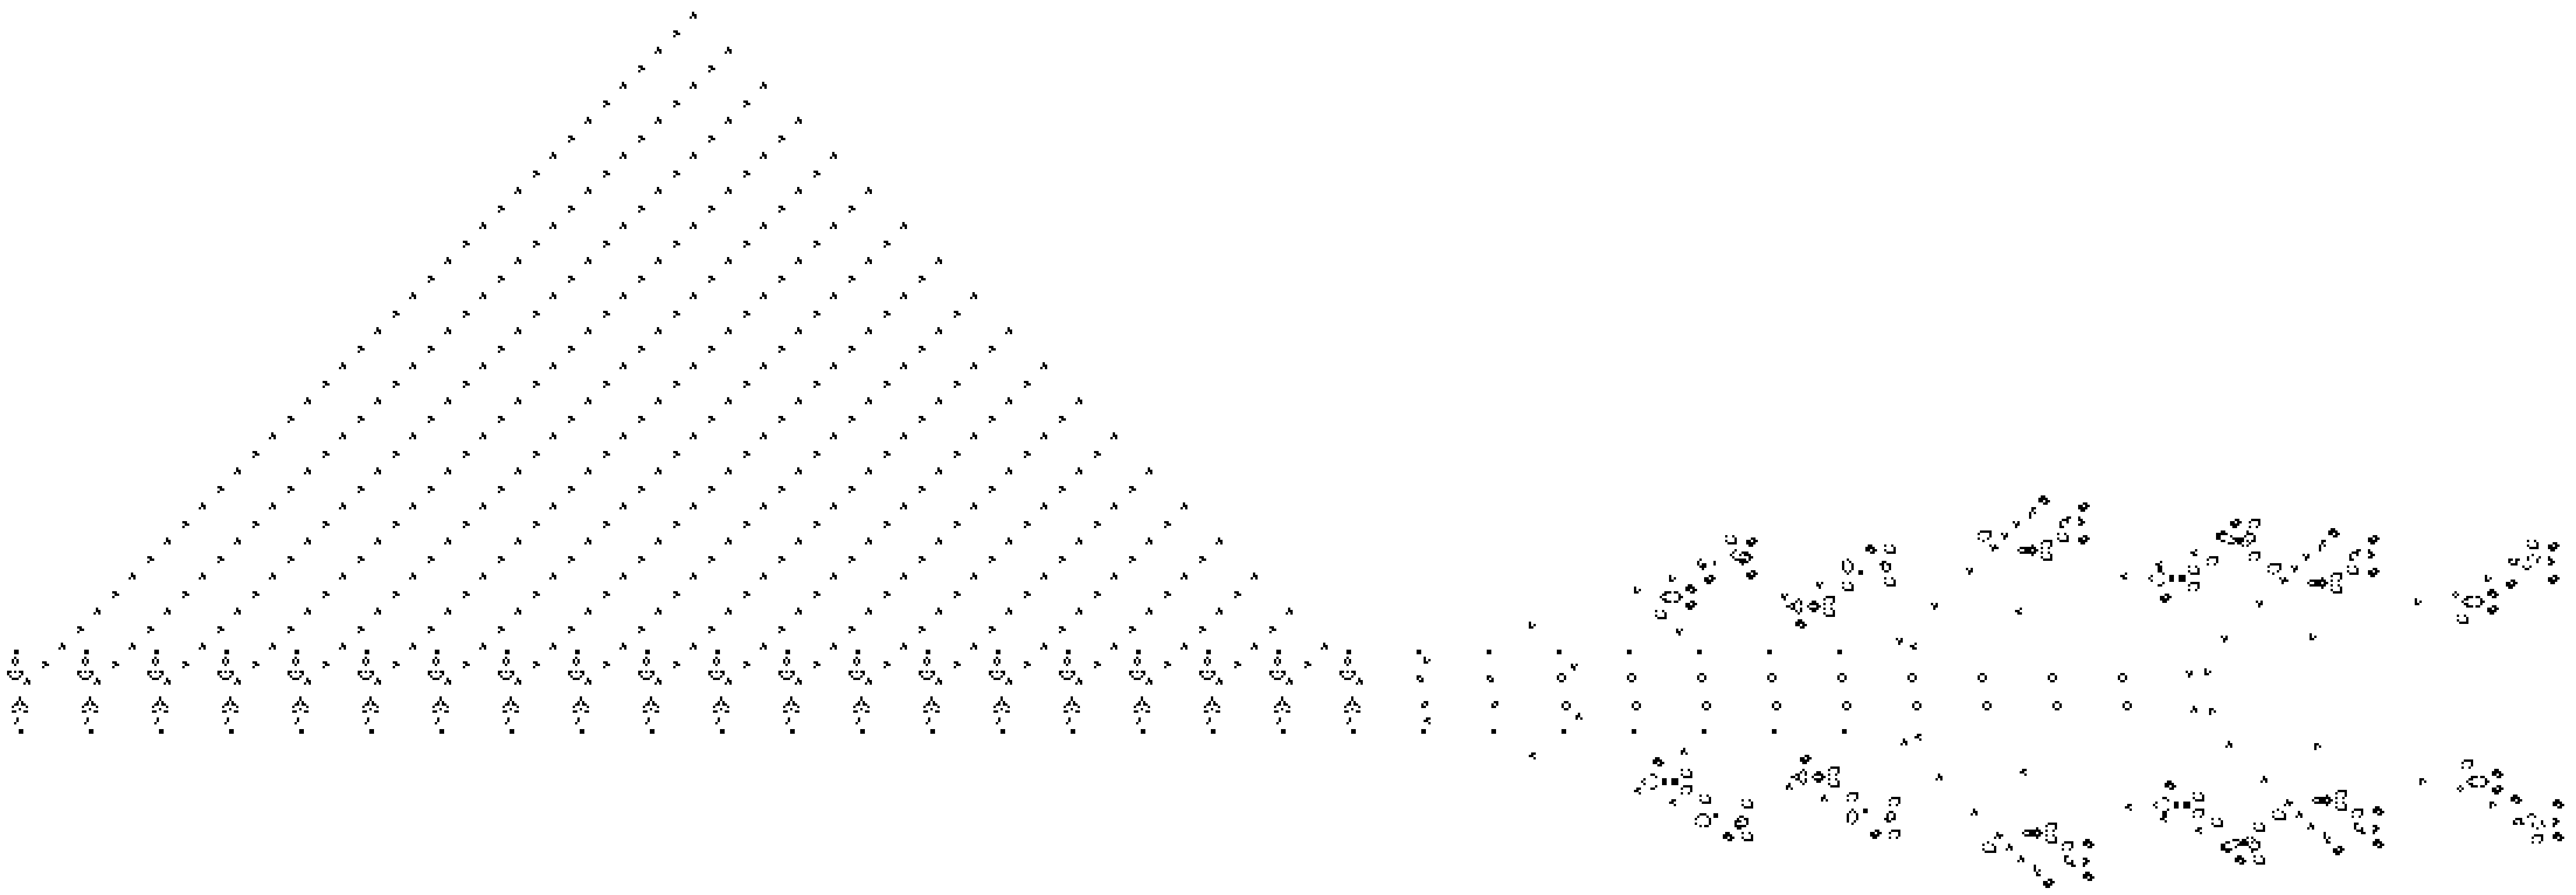
\includegraphics[width=\textwidth]{glider_synthesis/breeder_done_1200.png}
	\caption{After running the breeder for 1200~generations, we see a triangle of gliders form at the west, above the line of Gosper glider guns that has been synthesized. As the breeder moves farther to the east, the triangle continues to expand to the northeast.}\label{fig:breeder_done_1200}
\end{figure}

While this breeder is quite large, we have purposely not optimized it all, in order to make the mechanisms that make it work more apparent. The space rakes can be moved much closer to each other without compromising its functionality (see Exercise~\ref{exer:breeder_minimize}), and by cleverly manipulating the space rake debris it is actually possible to place more than one of the still lifes at the same time, thus halving the total number of space rakes from $12$ to $6$. We present and make use of a much more compact Gosper glider gun breeder that comes from these ideas a bit later, in Section~\ref{sec:primer_itself}.



\section{Slow Salvo Synthesis}\label{sec:slow_salvo}

In Section~\ref{sec:incremental_synthesis}, we saw that we can often break glider syntheses down into bits and pieces that are individually easy to understand and make use of. In this section, we take this idea to its most extreme by considering \emph{slow salvos}\index{salvo}, which are collections of gliders\footnote{Technically, a salvo can be made up of any spaceships, but the term almost always refers to gliders.} that (a) are \emph{slow}: only one glider interacts in the synthesis at a time, and (b) form a \emph{salvo}: all of the gliders come from the same direction.

In order for the gliders in a slow salvo to be able to actually synthesize anything, we need another object (called a \emph{seed}\index{seed}) for it to crash into. While we could in principle use any object, it is typical to use a block\index{block} as a starting point, since it is the simplest and most symmetric stationary object. Furthermore, it is typical to only consider either \emph{p1 slow salvos} or \emph{p2 slow salvos}, which are slow salvos in which the intermediate objects that are created after every glider collision are still lifes or some combination of still lifes and period~2 oscillators, respectively.\footnote{P2 salvos are advantageous because blinkers are so easy to synthesize, and we will see shortly that the clock\index{clock} is also a useful tool when working with slow salvos. We could analogously consider p$n$ slow salvos for some $n \geq 3$, but in practice not much is gained by doing so, since objects with period~3 or higher typically aren't any easier to create in intermediate stages of synthesis than objects period~1 or period~2.} This perhaps seems like quite an extensive list of restrictions, but we have in fact already seen a few objects that can be created via p1 slow salvos. For example, we saw in Table~\ref{tab:sequential_synth} that we could use a pond as a seed in a p1~slow salvo to produce a ship, and then a queen bee.% As a less trivial example, consider the p1 slow salvo synthesis presented in Figure~??, which uses a total of 12 gliders to gradually change the starting block into more and more complicated still lifes, eventually resulting in an eater~1. Compare this synthesis with the one presented in Figure~\ref{fig:17_cell_synthesis}, which was neither slow (multiple gliders are involved in most stages of synthesis) nor a salvo (gliders approach from all four directions).

Despite how restrictive slow salvos seem at first, it is a remarkable fact that they are exactly as general as standard glider syntheses. That is, if we can synthesize an object with gliders at all then we can synthesize it with a p2 slow salvo.\footnote{However, the slow salvo might contain considerably more gliders than other glider syntheses.} In order to pin down exactly why this is the case, we now introduce several new reactions that allow us to systematically create slow salvo syntheses from standard glider syntheses.


\subsection{Creating and Moving Blocks}\label{sec:slow_salvo_blocks}

Our first step toward showing that slow salvos can construct anything that regular glider syntheses can is to demonstrate how we can create almost any arrangement of any number of blocks in the Life plane that we like. The first reaction that we will need is the one displayed in Figure~\ref{fig:slow_salvo_splitter}, which uses a slow salvo of $2$ gliders to turn a single block into two blocks.

\begin{figure}[!htb]
	\centering\embedlink{slow_salvo_splitter}{\vcenteredhbox{\patternimg{0.101}{slow_salvo_splitter_0}} \vcenteredhbox{\gliderarrow{1}} \vcenteredhbox{\patternimg{0.101}{slow_salvo_splitter_1}} \vcenteredhbox{\gliderarrow{1}} \vcenteredhbox{\patternimg{0.101}{slow_salvo_splitter_2}}}
	\caption{A $2$-glider slow salvo can turn one block into two blocks.}\label{fig:slow_salvo_splitter}
\end{figure}

While the two resulting blocks are in very different positions than the initial block, it turns out that this does not particularly matter, as we can also use p1 slow salvos to move a block from one position on the Life plane to any other. To show that such a movement is possible, we use the two block-moving reactions displayed in Figure~\ref{fig:block_movers}. The first of these reactions uses a single glider to move a block up $2$~cells and left $1$~cell (in fact, this is exactly the (2,1) block pull\index{(2,1) block pull} that we saw way back in Figure~\ref{fig:glider_block_move}), and the second reaction uses six gliders (in a p1 slow salvo) to move a block down and to the right $1$ cell.

\begin{figure}[!htb]
	\centering
	\begin{tabular}{@{}cc@{}}
		\begin{subfigure}[b]{.39\textwidth}
			\centering\embedlink{block_move_1_glider}{\vcenteredhbox{\patternimg{0.176}{block_move_1_glider_0}} \vcenteredhbox{\gliderarrow{1}} \vcenteredhbox{\patternimg{0.176}{block_move_1_glider_1}}}
			\caption{The (2,1) block pull is a reaction in which a single glider pulls a block by $2$~cells in one direction and $1$~cell in the other.}\label{fig:block_move_1_glider}
		\end{subfigure} &
		\begin{subfigure}[b]{.59\textwidth}
			\centering\raisebox{-0.48\height}{\begin{tikzpicture}[scale=0.5, every node/.style={transform shape}]%
				\node[inner sep=0pt,anchor=south west] at (0,0) {\embedlink{block_move_6_gliders}{\patternimg{0.2}{block_move_6_gliders_0}}};
				
				\colorletternode{green}{5.8}{2.85}{1}
				\colorletternode{green}{4.7}{4.6}{2}
				\colorletternode{green}{5.8}{6.3}{3}
				\colorletternode{green}{2.3}{2.85}{4}
				\colorletternode{green}{1.65}{4.6}{5}
				\colorletternode{green}{0.3}{5.6}{6}
				\end{tikzpicture}} \patternlink{block_move_6_gliders}{\vcenteredhbox{\gliderarrow{6}} \vcenteredhbox{\patternimg{0.1}{block_move_6_gliders_6}}}
			\caption{A $6$-glider slow salvo moving a block down and right by $1$ cell.}\label{fig:block_move_6_gliders}
		\end{subfigure}
	\end{tabular}
	\caption{Two methods of moving a block around with p1 slow salvos. The order in which the gliders should come in is indicated by the \bgbox{greenpastel}{green} numbers---their exact timing does not matter, as long as they are far enough apart that each collision settles down before the next glider arrives. Repeating these slow salvos allows us to move a block to any position on the Life plane.}
	\label{fig:block_movers}
\end{figure}

If we repeat these two reactions then we can move a block a single cell up, down, left, or right. For example, to move a block up a single cell, we could perform the movement in Figure~\ref{fig:block_move_1_glider}, followed by the movement in Figure~\ref{fig:block_move_6_gliders} (for a total cost of $7$ gliders). Similarly:\smallskip

\begin{itemize}
	\item To move a block right by a single cell, we could perform the movement in Figure~\ref{fig:block_move_1_glider}, followed by the movement in Figure~\ref{fig:block_move_6_gliders} twice.\footnote{This requires a total of $13$ gliders, which is far from optimal---another p1 slow salvo is known that accomplishes the same movement via only $7$~total gliders. However, we are just interested in presenting the conceptually simplest method of moving blocks, not necessarily the most efficient one. Paul Chapman and Dave Greene put together an extensive table of the cheapest known block-moving slow salvos, which is available at \httpurl{b3s23life.blogspot.com/2004/09/glues-slow-salvo-block-move-table.html} (note that the values in their table assume that the gliders come from the bottom-right, rather than the top-left). A slightly more up-to-date table that makes use of p2 salvos rather than just p1 salvos is available at \httpsurl{conwaylife.com/forums/viewtopic.php?f=7\&t=1072\#p8182}.}\smallskip
	
	\item To move a block left by a single cell, we could perform the movement in Figure~\ref{fig:block_move_1_glider}, but reflected along the diagonal from the top-left to the bottom right. Then perform the movement in Figure~\ref{fig:block_move_6_gliders}.\smallskip
	
	\item To move a block down by a single cell, we could first move it left by a single cell and then perform the movement in Figure~\ref{fig:block_move_6_gliders}.\smallskip
\end{itemize}

Now that we know how to use p1 slow salvos to move a block by a single cell in any direction, we can easily repeat these reactions over and over until the block is moved to whatever position we desire.%\footnote{In slightly more mathematical language, what we have shown is that every point in $\mathbb{Z}^2$ is a positive linear combination of the vectors $(-1,2)$, $(-2,1)$, and $(1,-1)$.}
% Note that there are more efficient ways than this though


% IMPORTANT http://conwaylife.com/forums/viewtopic.php?f=2&t=918&p=7291&hilit=blockic#p7291
\subsection{One-Time Turners}\label{sec:slow_salvo_turners}

Just like we can use gliders to create and move blocks around the Life plane, we can also use blocks to move gliders around the Life plane. We can thus use a p1 slow salvo to create arrangements of blocks that then change the direction of other gliders in the salvo, thus creating salvos that come from multiple directions.

To be a bit more explicit, consider the arrangement of blocks presented in Figure~\ref{fig:one_time_turner}, which can be used to rotate a glider by 90 degrees, but is destroyed in the process (contrast this with reflectors like the Snark\index{Snark}, which rotate gliders but remain unchanged). Reflectors like this are called \emph{one-time turners}\index{one-time turner}, and they are one of the key ingredients that let us emulate arbitrary glider syntheses via slow salvos. There are also numerous other 90-degree one-time turners involving various numbers of blocks (and sometimes other small still lifes---see Exercise~\ref{exer:boat_one_time_turner}), but this turner involving just two blocks is perhaps the simplest, and for now it is enough for our purposes.

\begin{figure}[!htb]
	\centering\embedlink{one_time_turner}{\vcenteredhbox{\patternimg{0.14}{one_time_turner_0}} \vcenteredhbox{\genarrow{35}} \vcenteredhbox{\patternimg{0.14}{one_time_turner_35}}}
	\caption{A \emph{one-time turner} composed of two blocks that rotates a glider by 90 degrees and destroys the blocks at the same time.}\label{fig:one_time_turner}
\end{figure}

Importantly, because this one-time turner is made up of nothing other than blocks, we can construct it using a p1 slow salvo via the techniques that we developed in the previous section. An explicit $12$-glider p1 slow salvo that does the job (and also leaves us with an extra block that we can then use to construct additional turners) is displayed in Figure~\ref{fig:create_one_time_turner}. This salvo works by using 2 gliders to duplicate the initial block (as in Figure~\ref{fig:slow_salvo_splitter}), 8 gliders to move one of these blocks to a new position, and then 2 more gliders to duplicate this block again.% (and due to the clever way we repositioned the second block, this second duplication leaves a pair of blocks in exactly the one-time turner configuration).

\begin{figure}[!htb]
	\centering\raisebox{-0.5\height}{\begin{tikzpicture}[scale=0.518, every node/.style={transform shape}]%
	\node[inner sep=0pt,anchor=south west] at (0,-0.2) {\embedlink{create_one_time_turner}{\patternimg{0.195}{create_one_time_turner_0}}};
				
	\colorletternode{green}{4.2}{3.75}{1}
	\colorletternode{green}{4.15}{5.9}{2}
	\end{tikzpicture}} \patternlink{create_one_time_turner}{\vcenteredhbox{\gliderarrow{2}}} \raisebox{-0.5\height}{\begin{tikzpicture}[scale=0.518, every node/.style={transform shape}]%
	\node[inner sep=0pt,anchor=south west] at (0,-0.2) {\patternlink{create_one_time_turner}{\patternimg{0.195}{create_one_time_turner_2}}};
	
	\colorletternode{green}{3.07}{6.35}{1}
	\colorletternode{green}{1.69}{7}{2}
	\colorletternode{green}{2.15}{5}{3}
	\colorletternode{green}{1.47}{5.87}{4}
	\colorletternode{green}{0.61}{6.74}{5}
	\colorletternode{green}{0.15}{7.87}{6}
	\colorletternode{green}{1.73}{8.09}{7}
	\colorletternode{green}{1.02}{8.98}{8}
	\end{tikzpicture}} \patternlink{create_one_time_turner}{\vcenteredhbox{\gliderarrow{8}}} \raisebox{-0.5\height}{\begin{tikzpicture}[scale=0.518, every node/.style={transform shape}]%
	\node[inner sep=0pt,anchor=south west] at (0,-0.2) {\patternlink{create_one_time_turner}{\patternimg{0.195}{create_one_time_turner_10}}};
	
	\colorletternode{green}{5.05}{4.8}{1}
	\colorletternode{green}{5}{7}{2}
	\end{tikzpicture}} \patternlink{create_one_time_turner}{\vcenteredhbox{\gliderarrow{2}}} \raisebox{-0.5\height}{\begin{tikzpicture}[scale=0.518, every node/.style={transform shape}]%
	\node[inner sep=0pt,anchor=south west] at (0,-0.2) {\patternlink{create_one_time_turner}{\patternimg{0.195}{create_one_time_turner_12}}};
	\end{tikzpicture}}
	\caption{A 12-glider p1 slow salvo creating the one-time turner from Figure~\ref{fig:one_time_turner} (highlighted in \bgbox{magentaback}{magenta}) and leaving behind another block to create additional turners or other objects with. The first $2$ gliders duplicate the initial block via the reaction of Figure~\ref{fig:slow_salvo_splitter}, the next $8$ gliders move one of the blocks down and to the right, and then the final $2$ gliders duplicate that moved block.}% The order in which the gliders should come in is indicated by the \bgbox{greenpastel}{green} numbers---their exact timing does not matter, as long as they are far enough apart that each collision settles down before the next glider arrives.}
	\label{fig:create_one_time_turner}
\end{figure}

We can thus use a total of $13$ gliders in a p1 slow salvo ($12$~to create the one-time turner and $1$~to use and destroy it) to create $1$~glider in a perpendicular direction, while still having a block left over to perform additional constructions with. Using this technique, we are now able to emulate multi-directional glider syntheses via unidirectional syntheses.

For example, consider the four-glider syntheses of the clock\index{clock} that we saw in Table~\ref{tab:other_glider_synth}, which each use one glider coming from all four possible directions. A unidirectional synthesis of the clock can be constructed by using a p1 slow salvo to construct four one-time turners---one of the gliders does not need to be turned at all, two gliders need to be turned once each, and one glider needs to be turned twice---and then firing four gliders at the one-time turners with the proper timing. An explicit configuration of one-time turners that works is displayed in Figure~\ref{fig:unidirection_clock_synthesis}.\footnote{It is possible to create a p1 slow salvo that builds this arrangement of blocks by hand, but there are also computer scripts that automate this process---see Exercise~\ref{exer:create_clock_turners}.}

\begin{figure}[!htb]
	\centering\embedlink{unidirection_clock_synthesis}{\vcenteredhbox{\patternimg{0.1}{unidirection_clock_synthesis}} \vcenteredhbox{\genarrow{135}} \vcenteredhbox{\patternimg{0.1}{unidirection_clock_synthesis_135}}}
	\caption{One-time turners (which can be synthesized with a p1 slow salvo) can be used to allow unidirectional glider waves (like the one on the left) to emulate multi-directional glider syntheses (like the one on the right). The gliders on the right are in exactly the position of the clock synthesis that we saw in Table~\ref{tab:other_glider_synth}.}\label{fig:unidirection_clock_synthesis}
\end{figure}

Unfortunately, this construction does not give us a true p1 slow salvo for constructing a clock, since the final four gliders in the synthesis (i.e., the ones that hit the one-time turners) must be synchronized with each other---we are not free to space them arbitrarily far from one another. In order to fix this problem, we need to introduce some methods for using blocks to duplicate gliders and adjust their timing.


% http://conwaylife.com/forums/viewtopic.php?f=2&t=1512
% table of blockic splitters: http://conwaylife.com/forums/viewtopic.php?f=2&t=1065#p7661
\subsection{Splitters and Timing}\label{sec:slow_salvo_splitters}

The first ingredient that we need in order avoid having to send synchronized gliders at our one-time turners is a method of turning one glider into many gliders. Just like our one-time turner, we would like this pattern to be composed entirely of blocks, and we would like it to be cleanly destroyed during the glider-duplicating reaction. Patterns with these properties are called \emph{blockic splitters}\index{blockic splitter},\footnote{The term \emph{blockic} refers to the fact that it is composed entirely of blocks. There are also splitters (and one-time turners) made up of other still lifes (or even blinkers), but we do not consider them here since blocks are enough for our purposes.} and one example is provided in Figure~\ref{fig:one_time_splitter}.

\begin{figure}[!htb]
	\centering\embedlink{one_time_splitter}{\vcenteredhbox{\patternimg{0.15}{one_time_splitter_0}} \vcenteredhbox{\genarrow{202}} \vcenteredhbox{\patternimg{0.09}{one_time_splitter_202}}}
	\caption{A \emph{blockic splitter}, which uses three blocks to turn one glider into four gliders (while destroying the blocks in the process).}\label{fig:one_time_splitter}
\end{figure}

This splitter \emph{almost} gets us what we need---it lets us turn one glider into four, and we could chain multiple splitters together to turn one glider into as many as we desire. We can use one-time turners to move these gliders around the Life plane, with the intention of emulating multi-direction glider syntheses, but unfortunately we are faced with two brand new problems:\smallskip

\begin{itemize}
	\item The one-time turner that we introduced in Figure~\ref{fig:one_time_turner} preserves the glider's color,\index{glider!color} so we have no way of obtaining glider color combinations other than those provided to us by the splitter in Figure~\ref{fig:one_time_splitter} (in which the bottom-left glider has the same color as the input glider, whereas the other $3$ gliders have the opposite color). Since the $4$-glider synthesis of a clock uses $2$ gliders of each color, in order to make a slow salvo synthesis of the clock we would have to use this splitter multiple times and then use blocks to delete the excess gliders, which is quite wasteful.\smallskip
	
	\item The one-time turner from Figure~\ref{fig:one_time_turner} gives us no control over timing, and we need some way of making sure that all of the desired gliders in a given synthesis not only arrive at the right place, but also at the right time.\smallskip
\end{itemize}

Fortunately, there is a common solution to both of the above problems, and it is simply to introduce several new one-time turners. In particular, the numerous 180-degree one-time turners presented in Table~\ref{tab:180_degree_one_time_turners} are capable of either preserving or changing the color of a glider, and also offsetting its timing by any amount that we desire.%\footnote{This collection of 180-degree one-time turners was compiled by Dave Greene.}

\begin{table}[!ht]\vspace*{0.05in}
	\begin{center}		
		\begin{tabular}{Sc Sc Sc Sc Sc Sc Sc}
		    \toprule
		    & \multicolumn{4}{c}{Offset} \\  \cmidrule{2-5}
		    & $0$ & $1$ & $2$ & $3$ \\ \midrule
			\specialcell{Color-\\ Preserving} & \specialcell{\patternimg{0.12}{180_one_time_turner_0_0}} & \specialcell{\patternimg{0.12}{180_one_time_turner_0_1}} & \specialcell{\patternimg{0.12}{180_one_time_turner_0_2}} & \specialcell{\patternimg{0.12}{180_one_time_turner_0_3}} \\
			\specialcell{Color-\\ Changing} & \specialcell{\patternimg{0.12}{180_one_time_turner_1_0}} & \specialcell{\patternimg{0.12}{180_one_time_turner_1_1}} & \specialcell{\patternimg{0.12}{180_one_time_turner_1_2}} & \specialcell{\patternimg{0.12}{180_one_time_turner_1_3}} \\\cmidrule{2-5}
			& $4$ & $5$ & $6$ & $7$ \\\cmidrule{2-5}
			\specialcell{Color-\\ Preserving} & \specialcell{\patternimg{0.12}{180_one_time_turner_0_4}} & \specialcell{\patternimg{0.12}{180_one_time_turner_0_5}} & \specialcell{\patternimg{0.12}{180_one_time_turner_0_6}} & \specialcell{\patternimg{0.12}{180_one_time_turner_0_7}} \\
			\specialcell{Color-\\ Changing} & \specialcell{\patternimg{0.12}{180_one_time_turner_1_4}} & \specialcell{\patternimg{0.12}{180_one_time_turner_1_5}} & \specialcell{\patternimg{0.12}{180_one_time_turner_1_6}} & \specialcell{\patternimg{0.12}{180_one_time_turner_1_7}} \\\bottomrule
		\end{tabular}
		\caption{By using different 90-degree one-time turners together, we can create this collection of 180-degree one-time turners that lets us set a glider to any timing and color. In all cases, the input glider is highlighted in \bgbox{greenback}{green} and comes in from the top-left, while the location of the output glider exactly 200 generations later is highlighted in \bgbox{orangeback}{orange}. The boats are not required for the turners to function, but just serve to make it easier to line up multiple different turners.}\label{tab:180_degree_one_time_turners}
	\end{center}
\end{table}

In order to make use of these 180-degree one-time turners to put gliders in (almost) any \emph{position} that we want, we first simply use copies of the 90-degree one-time turner from Figure~\ref{fig:one_time_turner} and the 180-degree one-time turners with offset~0 from Table~\ref{tab:180_degree_one_time_turners}. Importantly, we always place at least one 180-degree turner in the path of each glider, even if it is not required to get its positioning right (we will need that 180-degree turner to get the timing right momentarily).

Even though the positioning of the gliders is now correct, their timing will likely be horribly wrong. To fix this problem, we now focus on the glider that gets to its destination last---we will synchronize all of the other gliders with this one. To slow down those other gliders, we note that moving a 180-degree turner $1$ cell farther away causes the glider to reach its destination $8$ generations later (it now has to travel $1$ cell, and thus $4$ generations, farther in both directions). To delay a glider by $n$ generations, we can thus move its 180-degree turner farther away by $\lfloor n/8 \rfloor$ generations and then replace it by the turner from Table~\ref{tab:180_degree_one_time_turners} that has the same effect on its color but has offset $n \ \text{mod} \ 8$.

We now have a complete set of glider-preserving or glider-changing turners capable of delaying a glider by any of $0,1,2,\ldots,7$ generations.  So we have all the tools we need to position \emph{and} time gliders as we see fit. An example of how we can use the $4$ gliders produced by the splitter in Figure~\ref{fig:one_time_splitter} to synthesize a clock is presented in Figure~\ref{fig:clock_slow_salvo}. Note that we placed a 180-degree one-time turner in the path of each of the four gliders so that we could use the technique for correcting their timing described in the previous paragraph, and since each of those 180-degree turners is simply made up of two 90-degree one-time turners, we are able to separate their two halves in order to more easily control the glider's output position.

\begin{figure}[!htb]
	\centering
	\patternimglinkwidth{\textwidth}{clock_slow_salvo}
	\caption{A \emph{blockic seed} for a clock: The blockic splitter at the top-center (highlighted in \bgbox{orangeback2}{orange}) turns the single incoming glider into four gliders whose paths are outlined in \bgbox{yellowback2}{yellow}, \bgbox{greenpastel}{green}, \bgbox{aquaback}{aqua}, and \bgbox{magentaback}{magenta}. Those gliders are repeatedly reflected via one-time turners in such a way that they end up in the indicated positions required to synthesize a clock after $537$ generations. We could probably get away with using fewer one-time turners, but by placing a 180-degree turner in the path of every glider it is much easier to get their timing right.}
	\label{fig:clock_slow_salvo}
\end{figure}

A configuration of simple still lifes, like the one in Figure~\ref{fig:clock_slow_salvo}, that synthesizes an particular object when hit by a glider (or gliders) is called a \emph{seed}\index{seed} (and a seed made up entirely of blocks is called a \emph{blockic seed}).\index{blockic seed} Seeds are particularly useful since they immediately give us a p1 slow salvo for constructing an object---a clock in this case---since we ``just'' have to use a p1 slow salvo to construct the still lifes in the seed and then fire one additional glider to trigger the synthesis.

However, actually building a slow salvo synthesis for a seed is a tedious process. The $31$-block seed for a clock from Figure~\ref{fig:clock_slow_salvo} requires hundreds of slow gliders to construct (see Exercise~\ref{exer:create_clock_turners_nonsync})---recall that we already needed 12 gliders just to create a single $2$-block one-time turner in Figure~\ref{fig:create_one_time_turner}. For this reason, slow salvo syntheses of seeds are typically built by computer scripts, with \emph{slsparse}\index{slsparse}\index{slmake|see {slsparse}} (see \httpsurl{conwaylife.com/wiki/Slsparse} for tutorials and a download link) being the most widely used.% Even very small syntheses can require hundreds or thousands of gliders to emulate in a p1 slow salvo.\footnote{As an example, Dave Greene constructed an explicit p1 slow salvo consisting of 997 gliders that constructs a configuration of 81 blocks that, when hit by one additional glider, transforms into an 8-glider synthesis of the loafer\index{loafer} spaceship. This salvo can be seen at \httpsurl{conwaylife.com/forums/viewtopic.php?f=2\&t=1006\&p=7574\#p7574}.}


\subsection{Tight Packings of Gliders}\label{sec:slow_salvo_tight}

There is still one final problem that might arise when trying to emulate an arbitrary glider synthesis via a slow salvo synthesis, and that is the fact that some syntheses involve packings of gliders coming from the same direction that are too close together for us to place with our one-time turners. This was not a problem for the clock synthesis in Figure~\ref{fig:clock_slow_salvo} since each of the gliders in the synthesis comes from a different direction. However, if we were to try to use a p1 slow salvo to emulate the 3-glider synthesis of a HWSS displayed in Table~\ref{tab:3_glider_synth}, it is not obvious that we can position the two gliders that are heading southwest close enough to each other (since one of the gliders might interfere with any one-time turner that we try to use to position the other glider). To fix this glider-packing problem, we introduce one final reaction: the \emph{clock inserter}\index{clock!inserter},\footnote{Found by Martin Grant in December 2014.} which uses two opposing gliders to transform a clock\index{clock} into a perpendicular glider, as in Figure~\ref{fig:clock_inserter}.

\begin{figure}[!htb]
	\centering
	\embedlink{clock_inserter}{\vcenteredhbox{\phantom{$\cdots$ \genarrow{1}}} \vcenteredhbox{\patternimg{0.1}{clock_inserter_0}} \vcenteredhbox{\genarrow{1}} \vcenteredhbox{\patternimg{0.1}{clock_inserter_1}} \vcenteredhbox{\genarrow{1}} \vcenteredhbox{\patternimg{0.1}{clock_inserter_2}} \vcenteredhbox{\genarrow{1}} \vcenteredhbox{\patternimg{0.1}{clock_inserter_3}} \vcenteredhbox{\phantomarrowa{} $\cdots$} \\[1em]
		\vcenteredhbox{$\cdots$ \genarrow{1}} \vcenteredhbox{\patternimg{0.1}{clock_inserter_4}} \vcenteredhbox{\genarrow{1}} \vcenteredhbox{\patternimg{0.1}{clock_inserter_5}} \vcenteredhbox{\genarrow{1}} \vcenteredhbox{\patternimg{0.1}{clock_inserter_6}} \vcenteredhbox{\genarrow{1}} \vcenteredhbox{\patternimg{0.1}{clock_inserter_7}} \vcenteredhbox{\phantom{\phantomarrowa{} $\cdots$}}}
	\caption{The \emph{clock inserter} is a reaction that very cleanly collides two gliders in such a way as to transform a clock into a perpendicular glider. The two-glider collision produces a domino spark in generation~5 (shown in \bgbox{redback}{red}) and then dies off, while the domino spark\index{domino spark} initiates the clock-to-glider transformation. The debris at the bottom-right in generation~8 dies off in 5 more generations.}\label{fig:clock_inserter}
\end{figure}

The key facts that make this reaction so useful for us are (1) that the output glider appears at a small offset and moves through the space just vacated by the colliding input gliders, and (2) the reaction is almost effortless---it does not disrupt any other cells around the clock and output glider, and thus does not disrupt other nearby gliders either. This reaction can thus be used to place a glider very close in front of, or to the side of, another already-placed glider (see Figure~\ref{fig:clock_inserter_effective} for an illustration of how closely it can place a new glider to other gliders). Because of this, we can use this reaction to build any arrangement of gliders, no matter how tight, as long as we start by placing the gliders in the back first. Actually \emph{proving} that the clock inserter reaction can be used to build any arrangement of gliders is somewhat technical and messy,\footnote{Chris Cain wrote a script that automatically uses clock inserters to build glider arrangements in 2014, and then he and Dave Greene used the script to build such a wide array of tight glider arrangements that this could probably be considered the first proof that p2 slow salvos can build any configuration of gliders. Cain's script can be found at \httpsurl{conwaylife.com/forums/viewtopic.php?f=2\&t=1512\&start=25\#p15133}.} since there are many possible ways for gliders to be near each other, so we defer the proof to Appendix~\ref{chp:appendix_salvo}.

With this reaction in hand, we can now use a p2 slow salvo to construct any arrangement of gliders in the plane that we desire. First, we ``rewind'' the desired glider synthesis back as far as we like, so that it consists of four salvos of gliders---one coming from each direction.\footnote{Recall that the gliders must be able to reach their positions from arbitrarily far away in order to be considered a valid glider synthesis.} We then construct the four salvos one glider at a time. If the gliders in a salvo are spaced sufficiently far apart, we can insert gliders into it via one-time turners. If the gliders are spaced close together, we instead first synthesize a clock (via p1 slow salvo synthesis, such as in Figure~\ref{fig:clock_slow_salvo}) and then use the clock inserter to insert the close gliders one at a time. We have thus finally proved the following theorem:

\begin{theorem}\label{thm:p2_slow_salvo}
	Every pattern that can be constructed via glider synthesis can be constructed by a p2 slow salvo glider synthesis.
\end{theorem}

\begin{figure}[!htb]
	\centering
	\embedlink{clock_inserter_effective}{\vcenteredhbox{\patternimg{0.115}{clock_inserter_effective_0}} \vcenteredhbox{\genarrow{52}} \vcenteredhbox{\patternimg{0.115}{clock_inserter_effective_52}}}
	\caption{A demonstration of how the clock inserter (shown in \bgbox{greenback}{green} on the left) can be used to place a glider (shown in \bgbox{orangeback}{orange} on the right) closely beside and in front of other already-placed gliders.}\label{fig:clock_inserter_effective}
\end{figure}

The only p2 object that we needed to prove Theorem~\ref{thm:p2_slow_salvo} was the clock, which we used to place clusters of tightly-packed gliders. We can get around having to use clocks (and thus avoid p$2$ objects altogether) by instead using the blockic seed of a clock from Figure~\ref{fig:clock_slow_salvo}. More specifically, if we wish to use a clock insertion reaction, we first split a single glider into three via blockic splitters---one of those gliders then hits the seed, creating a clock, and the other two are reflected so as to trigger the clock insertion reaction as in Figure~\ref{fig:clock_inserter}. Since this entire process is carried out by a single glider in the slow salvo synthesis, the result is a p1 slow salvo synthesis. We thus have the following strengthening of Theorem~\ref{thm:p2_slow_salvo}:\footnote{There are some mild technicalities that we have glossed over here---see Exercise~\ref{exer:p2_salvo_reduce_to_p1}.}%\footnote{The fact that some p2 clocks are created during this synthesis is irrelevant, since they are destroyed before the next glider in the salvo arrives.}

\begin{theorem}\label{thm:p1_slow_salvo}
	Every pattern that can be constructed via glider synthesis can be constructed by a p1 slow salvo glider synthesis.
\end{theorem}


% http://conwaylife.com/forums/viewtopic.php?f=2&t=1512&start=25#p23670
% IMPORTANT: http://conwaylife.com/forums/viewtopic.php?f=2&t=1006&p=7574#p7574
%% Last 15-bit SL: http://conwaylife.com/forums/viewtopic.php?f=2&t=1155&start=75#p9258
%% Last 16-bit SL: http://conwaylife.com/forums/viewtopic.php?f=2&t=1155&start=225#p10227
%% Last 17-bit SL: http://conwaylife.com/forums/viewtopic.php?f=2&t=1276&start=100#p11972
%% Last 18-bit SL: http://conwaylife.com/forums/viewtopic.php?f=2&t=1467&start=50#p14272
%% 5-glider very long snake: http://conwaylife.com/forums/viewtopic.php?f=2&t=1452&p=17219#p17102
%%%%%%%%%%%%%%%%%%%%%%%%%%%%%%%%
\section{Notes and Historical Remarks}\label{sec:synthesis_notes}
%%%%%%%%%%%%%%%%%%%%%%%%%%%%%%%%

The importance of glider synthesis was known essentially as soon as the glider itself was found in 1970, with common folklore being that we could send gliders as signals throughout the Life plane and collide those gliders in different ways to simulate arbitrary computations. This basic idea has been refined and made more precise repeatedly over the past 50 years, to the point that there are now explicit patterns that do exactly this---they collide gliders so as to perform arbitrary computations and build almost any pattern of our choosing (we will delve deeply into the specifics of how these patterns work in Chapters~\ref{chp:universal_computation} and~\ref{chp:universal_construction}).

The first specific and explicit uses of glider syntheses were demonstrated in 1971, when Bill Gosper constructed the first breeder (essentially the breeder that we built in Section~\ref{sec:gosper_breeder}) as well as the first lightweight and middleweight spaceship guns. These patterns demonstrated the kind of leap in complexity that is possible when taking advantage of glider synthesis, and it led to a surge in interest in the topic over the following years.

By 1973, the majority of ``basic'' Life objects were synthesizable, including lightweight, middleweight, and heavyweight spaceships, switch engines (and their block-laying and glider-producing counterparts), commonly-occurring oscillators like the pentadecathlon and pulsar, and all still lifes and oscillators with 7 or fewer cells other than the clock and the long snake. Syntheses of larger composite patterns were even being discovered by this point, with Douglas Petrie constructing the $11$-glider synthesis of the Schick engine displayed in Figure~\ref{fig:schick_engine_synth} in 1973. The majority of these early syntheses were developed by David Buckingham, Mark Niemiec, and Douglas Petrie.

Over the following decades, David Buckingham continued to develop syntheses for still lifes and oscillators, and he completed syntheses of all of them with $14$ or fewer cells by no later than 1992. His technique was to make heavy use of incremental synthesis, building the objects from the inside out, only using a couple of gliders at a time to tweak the outermost portion of the object that he was synthesizing. This method works very well when synthesizing objects that have ``end pieces'' like tails that can be removed or altered without affecting the pattern's stability. However, compact still lifes like the one in Figure~\ref{fig:14_cell_synth} are much more difficult to construct, and this particular still life (which was the last $14$-cell still life to be synthesized) was initially synthesized using a massive incremental synthesis involving more than $30$ gliders.

\begin{figure}[!htb]
	\centering
	\begin{subfigure}{.135\textwidth}
		\centering\patternimglink{0.135}{14_cell_synth}
		\caption{$14$ cells.}\label{fig:14_cell_synth}
	\end{subfigure} \ \ \ \ % 
	\begin{subfigure}{.135\textwidth}
		\centering\patternimglink{0.135}{15_cell_synth}
		\caption{$15$ cells.}\label{fig:15_cell_synth}
	\end{subfigure} \ \ \ \ % 
	\begin{subfigure}{.13\textwidth}
		\centering\patternimglink{0.135}{16_cell_synth}
		\caption{$16$ cells.}\label{fig:16_cell_synth}
	\end{subfigure} \ \ \ \ % 
	\begin{subfigure}{.14\textwidth}
		\centering\patternimglink{0.135}{17_cell_synth}
		\caption{$17$ cells.}\label{fig:17_cell_synth}
	\end{subfigure} \ \ \ \ % 
	\begin{subfigure}{.14\textwidth}
		\centering\patternimglink{0.135}{18_cell_synth}
		\caption{$18$ cells.}\label{fig:18_cell_synth}
	\end{subfigure} \ \ \ \ % 
	\begin{subfigure}{.145\textwidth}
		\centering\patternimglink{0.12161157024}{19_cell_synth}
		\caption{$19$ cells.}\label{fig:19_cell_synth}
	\end{subfigure}
	\caption{The final still lifes with $14$--$19$ cells to be synthesized by gliders.}\label{fig:hard_to_synth_sls}
\end{figure}

Mark Niemiec continued on with this work, creating a large database that he used to automatically generate syntheses of thousands of still lifes by piecing together known reactions \cite{Nie03,Nie10}. This greatly reduced the number of still life syntheses that needed to be found by hand, and in 2013 he completed syntheses of all $15$-cell still lifes (as well as syntheses for all except for a few hundred 16-, 17-, and 18-cell still lifes).

\begin{figure}[!htb]
	\centering
	\embedlink{17_cell_synthesis}{\vcenteredhbox{\phantom{$\cdots$ \gliderarrow{2}}} \vcenteredhbox{\patternimg{0.12}{17_cell_1}} \vcenteredhbox{\gliderarrow{4}} \vcenteredhbox{\patternimg{0.12}{17_cell_2}} \vcenteredhbox{\gliderarrow{2}} \vcenteredhbox{\patternimg{0.12}{17_cell_3}} \vcenteredhbox{\gliderarrow{2}} \vcenteredhbox{\patternimg{0.12}{17_cell_4}}} \\[1em]
	
	\patternlink{17_cell_synthesis}{\vcenteredhbox{$\cdots$ \gliderarrow{2}} \vcenteredhbox{\patternimg{0.12}{17_cell_5}} \vcenteredhbox{\gliderarrow{4}} \vcenteredhbox{\patternimg{0.12}{17_cell_6}} \vcenteredhbox{\gliderarrow{6}} \vcenteredhbox{\patternimg{0.12}{17_cell_7}} \vcenteredhbox{\gliderarrow{2}} \vcenteredhbox{\patternimg{0.12}{17_cell_8}}} \\[1em]
	
	\patternlink{17_cell_synthesis}{\vcenteredhbox{$\cdots$ \gliderarrow{5}} \vcenteredhbox{\patternimg{0.12}{17_cell_9}} \vcenteredhbox{\gliderarrow{3}} \vcenteredhbox{\patternimg{0.12}{17_cell_10}} \vcenteredhbox{\gliderarrow{4}} \vcenteredhbox{\patternimg{0.12}{17_cell_11}} \vcenteredhbox{\gliderarrow{2}} \vcenteredhbox{\patternimg{0.12}{17_cell_12}}} \\[1em]
	
	\patternlink{17_cell_synthesis}{\vcenteredhbox{$\cdots$ \gliderarrow{1}} \vcenteredhbox{\patternimg{0.12}{17_cell_13}} \vcenteredhbox{\gliderarrow{5}} \vcenteredhbox{\patternimg{0.12}{17_cell_14}} \vcenteredhbox{\gliderarrow{7}} \vcenteredhbox{\patternimg{0.12}{17_cell_15}} \vcenteredhbox{\gliderarrow{5}} \vcenteredhbox{\patternimg{0.12}{17_cell_16}}} \\[1em]
	
	\patternlink{17_cell_synthesis}{\vcenteredhbox{$\cdots$ \gliderarrow{3}} \vcenteredhbox{\patternimg{0.12}{17_cell_17}} \vcenteredhbox{\gliderarrow{2}} \vcenteredhbox{\patternimg{0.12}{17_cell_18}} \vcenteredhbox{\gliderarrow{8}} \vcenteredhbox{\patternimg{0.12}{17_cell_19}} \vcenteredhbox{\gliderarrow{9}} \vcenteredhbox{\patternimg{0.12}{17_cell_20}}} \\[1em]
	
	\patternlink{17_cell_synthesis}{\vcenteredhbox{$\cdots$ \gliderarrow{2}} \vcenteredhbox{\patternimg{0.12}{17_cell_21}} \vcenteredhbox{\gliderarrow{2}} \vcenteredhbox{\patternimg{0.12}{17_cell_22}} \vcenteredhbox{\gliderarrow{10}} \vcenteredhbox{\patternimg{0.12}{17_cell_23}} \vcenteredhbox{\gliderarrow{4}} \vcenteredhbox{\patternimg{0.12}{17_cell_24}}}
	
	\caption{A summary of a massive $94$-glider incremental synthesis of a hard-to-construct 17-cell still life (shown at the bottom right). Each stage in the synthesis works by using a glider collision to transform one still life into another. The cells that were created or modified in the previous step of the synthesis are shown in \bgbox{redback}{red}, and the gliders that will be involved in the next collision are shown in \bgbox{greenback}{green}.}\label{fig:17_cell_synthesis}
\end{figure}

Glider syntheses for the remaining 16-cell still lifes were then found via a collaborative effort on the ConwayLife.com forums, mostly led by Martin Grant, Matthias Merzenich, and Mark Niemiec, with the final synthesis (see Figure~\ref{fig:16_cell_synth}) being completed in January 2014. Another five-month collaborative effort, led by the same group of people, completed syntheses of the 17-cell still lifes in May 2014. A comparatively quick two-month effort finished the remaining syntheses of 18-cell still lifes in November of that year, and then a final four-month effort resulted in the synthesis of the last $930$ or so 19-cell still lifes in February 2020.

To give an idea of the size of this achievement, recall from Table~\ref{tab:small_still_lifes} that there are 78,297 different strict still lifes with 19 or fewer cells. Not only is this a huge number of distinct objects to synthesize, but the syntheses themselves are often monstrously large. For example, Figure~\ref{fig:17_cell_synthesis} shows how one of the ``problematic'' 17-cell still lifes was constructed by using a whopping total of 94 gliders and over 20 stages of incremental synthesis.

Rather than trying to push these techniques to synthesize all still lifes with 20 live cells, focus has shifted somewhat to trying to reduce the number of gliders required to synthesize these objects. It has been known for decades how to synthesize all still lifes with $8$ or fewer cells via $4$ or fewer gliders. Similarly, glider syntheses are known for constructing every still life with $9, 10, 11, 12,$ and $13$ live cells via $5, 9, 9, 11,$ and $12$ or fewer gliders, respectively.\footnote{It was not known how to synthesize the $9$-cell long$^3$ snake\index{long$^3$ snake} with fewer than $6$ gliders until February 2015, when Matthias Merzenich derived a $5$-glider synthesis from an apgsearch\index{apgsearch} soup.} Recent efforts have attempted to continue this pattern and synthesize all small still lifes in fewer than $1$ glider per live cell. This project was completed for $14$-, $15$-, $16$-, and $17$-cell still lifes in October 2016, November 2016, May 2017, and September 2019, respectively. For example, we now know how to construct the $17$-cell still life from Figure~\ref{fig:17_cell_synthesis} (which was first synthesized by $94$ gliders) via just $10$ gliders---see Figure~\ref{fig:17_cell_synthesis_small}.

\begin{figure}[!htb]
	\centering
	\embedlink{17_cell_synthesis_small}{\vcenteredhbox{\patternimg{0.12}{17_cell_synthesis_small_0}} \vcenteredhbox{\gliderarrow{9}} \vcenteredhbox{\patternimg{0.12}{17_cell_synthesis_small_1}} \vcenteredhbox{\gliderarrow{1}} \vcenteredhbox{\patternimg{0.12}{17_cell_synthesis_small_2}}}
	\caption{A $10$-glider synthesis of the $17$-cell still life from Figure~\ref{fig:17_cell_synthesis} that was constructed with the help of a soup that was found by apgsearch.}\label{fig:17_cell_synthesis_small}
\end{figure}

Remarkably, it was even shown in September 2020 that every glider-synthesizable still life can be synthesized via $17$ or fewer gliders---see Section~\ref{sec:universal_construction_history}. However, it remains an open question whether or not every still life (or every oscillator, or even every pattern that has predecessors) is actually glider-synthesizable. Closely related is the (also open) question of whether or not there exists a still life whose only parent is itself.\footnote{For the purposes of this problem, a still life together with far away non-interacting dying ash is not considered a different parent than just the still life itself. Conway offered a \$50 prize for a solution to this problem in October 1972, which has gone unclaimed to this day.} Finding such a pattern would answer both of these questions, since if a still life's only parent is itself then it can not be constructed via glider synthesis (or any other means).


% TODO(?): Mention more-or-less complete recent computer search for 3-glider syntheses and recently found such syntheses
% One-time glider to LWSS: http://conwaylife.com/forums/viewtopic.php?f=2&t=1134&p=8489#p8488
% one-time LWSS turner: http://conwaylife.com/forums/viewtopic.php?f=2&t=1134&p=8489#p8519
%%%%%%%%%%%%%%%%%%%%%%%%%%%%%%%%%
\section*{Exercises \hfill \normalfont\textsf{\small solutions to starred exercises on \hyperlink{solutions_glider_synthesis}{page \pageref{solutions_glider_synthesis}}}}
\label{sec:synthesis_exercises}
\addcontentsline{toc}{section}{Exercises}
\vspace*{-0.4cm}\hrulefill\vspace*{-0.3cm}\footnotesize\begin{multicols}{2}\vspace*{-0.4cm}\raggedcolumns\interlinepenalty=10000
\setlength{\parskip}{0pt}
%%%%%%%%%%%%%%%%%%%%%%%%%%%%%%%%%

\begin{problemstar}\label{exer:glider_cleanup}
	Many glider syntheses work by using a small number of gliders to create the desired object plus some debris, and then additional gliders to clean up the debris. In each of the following syntheses, identify which gliders are used to clean up debris.
	\begin{enumerate}[label=\bf\color{ocre}(\alph*)]
		\item \raisebox{-\height+0.5em}{\patternimglink{0.1}{exercise_glider_cleanup_1}}
		\item \raisebox{-\height+0.5em}{\patternimglink{0.1}{tumbler_synthesis}}
		\item \raisebox{-\height+0.5em}{\patternimglink{0.1}{snacker_synthesis}}\\
	\end{enumerate}
\end{problemstar}


\mfilbreak


\begin{problem}\label{exer:single_glider_cleanup}
	Gliders can be used to destroy essentially any unwanted debris that is left over after a synthesis. Use a single glider to destroy each of the following objects (and also destroy the glider in the process):
	\begin{enumerate}[label=\bf\color{ocre}(\alph*)]
		\item A block.
		
		\item A beehive.
		
		\item A blinker.
		
		\item A ship.
		
		\item An LWSS.
	\end{enumerate}
\end{problem}


\mfilbreak


\begin{problem}\label{exer:multiple_glider_cleanup}
	Use multiple gliders to completely destroy each of the following objects.
	
	\noindent [Hint: Use one or two gliders to break the object down into simple ash objects like those from Exercise~\ref{exer:single_glider_cleanup} and then use additional gliders to clean up those simpler objects.]
	\begin{enumerate}[label=\bf\color{ocre}(\alph*)]
		\item A queen bee shuttle.
		
		\item A copperhead.
		
		\item Rich's p16.
	\end{enumerate}
\end{problem}


\mfilbreak


\begin{problemstar}\label{exer:glider_block_collisions}
	There are exactly $6$~distinct ways for a glider to collide with a block. List them all and describe the result of each collision.
\end{problemstar}
% pi, honey farm, move block, final 3 annihilate both glider and block


\mfilbreak


\begin{problemstar}\label{exer:twit_synthesis}
	Use the syntheses from this chapter to create a 7-glider synthesis of eater~5\index{eater!5}.
\end{problemstar}


\mfilbreak


% Solution: p60_lwss_backrake.txt
\begin{problem}\label{exer:p60_lwss_backrake}
	Use a lightweight spaceship synthesis from this chapter to construct a backrake that creates a period~$120$ stream of lightweight spaceships.
\end{problem}


\mfilbreak


\begin{problem}\label{exer:mwss_gun}
	Use three Gosper glider guns to create a middleweight spaceship gun.
\end{problem}


\mfilbreak


\begin{problem}\label{exer:hwss_gun}
	Consider the heavyweight spaceship synthesis in Table~\ref{tab:3_glider_synth}.
	\begin{enumerate}[label=\bf\color{ocre}(\alph*)]
		\item Why can't you use three Gosper glider guns and this synthesis to create a heavyweight spaceship gun?
		
		\item One way to overcome this problem is to use \emph{glider pushers}\footnote{Found by Dietrich Leithner in December 1993.}\index{glider!pusher} (displayed below) to repeatedly push one glider stream closer to another. How many glider pushers would you need to use to fix the problem from part~(a)?\smallskip
				
		\begin{minipage}{\linewidth}
			\centering
			\patternimglink{0.1}{glider_pusher}
		\end{minipage}
	\end{enumerate}
\end{problem}


\mfilbreak


\begin{problem}\label{exer:queen_bee_synth}
	Use a two-glider synthesis of a block and a three-glider synthesis of a queen bee to create a $7$-glider synthesis of a queen bee shuttle\index{queen bee!shuttle}.
\end{problem}


\mfilbreak


\begin{problem}\label{exer:twin_bee_shuttle_synth}
	Consider the four-glider synthesis of the twin bees\index{twin bees} presented in Figure~\ref{tab:other_glider_synth}.\smallskip
	
	\begin{enumerate}[label=\bf\color{ocre}(\alph*)]
		\item Use this synthesis to synthesize a twin bees shuttle.
		
		\item Use this synthesis to synthesize the twin bees gun from Figure~\ref{fig:twin_bees_gun}.
	\end{enumerate}
\end{problem}


\mfilbreak


\begin{problem}\label{exer:synthesize_glider_pusher}
	Create a glider synthesis of the glider pusher from Exercise~\ref{exer:hwss_gun}.
\end{problem}


\mfilbreak


\begin{problem}\label{exer:oscillator_syntheses}
	Construct a glider synthesis of the period~36 oscillator from Figure~\ref{fig:period_36}.
\end{problem}


\mfilbreak


% TODO: double check switch engine synth here uses 3-glider synth, not 4
\begin{problemstar}\label{exer:glider_synth_two_directions}\index{kickback reaction}
	By using the $2$-glider \emph{kickback reaction} from Table~\ref{tab:2_glider_synth} that changes the direction of a glider, we can decrease the number of directions used in many glider syntheses at the expense of increasing the number of gliders required. Use this technique to create glider syntheses for each of the following patterns with the property that all gliders come from just two different directions.
	\begin{enumerate}[label=\bf\color{ocre}(\alph*)]
		\item A switch engine.\index{switch engine}
		
		\item A clock.\index{clock}
		
		\item A $3$-engine Cordership.\index{Cordership}
	\end{enumerate}
\end{problemstar}


\mfilbreak


\begin{problemstar}\label{exer:2_engine_cordership_synthesis}
	Recall the $2$-engine Cordership from Exercise~\ref{exer:2_engine_cordership}.\smallskip
	
	\begin{enumerate}[label=\bf\color{ocre}(\alph*)]
		\item Construct a glider synthesis of this Cordership.
		
		\item Construct a glider synthesis of this Cordership that uses gliders coming only from two different directions.
		
		\noindent [Hint: Refer back to Exercise~\ref{exer:glider_synth_two_directions}.]
	\end{enumerate}
\end{problemstar}


\mfilbreak


\begin{problemstar}\label{exer:glider_synth_tee}
	By using the $3$-glider \emph{tee}\index{tee} collision from Table~\ref{tab:3_glider_synth}, which produces a glider perpendicular to each of the input gliders, we can modify many glider syntheses so that all input gliders come from two directions that are opposite each other. Use this technique to create glider syntheses of each of the following patterns, with the property that all gliders come from two opposing directions.
	\begin{enumerate}[label=\bf\color{ocre}(\alph*)]
		\item A switch engine.
		
		\item A clock.
		
		\item Twin bees.
	\end{enumerate}
\end{problemstar}


\mfilbreak


\begin{problem}\label{exer:ggg_stabilized_by_eater_synthesis}
	Construct a glider synthesis for a Gosper glider gun that is stabilized on one end by an eater~$1$ instead of a block (as in the buckaroo of Figure~\ref{fig:buckaroo}).
\end{problem}


\mfilbreak


\begin{problem}\label{exer:ecologist_synth}
	For incremental syntheses of moving objects, like this ecologist from Figure~\ref{fig:ecologist_synth_b}, there tend to be more choices to be made, since individual components may be constructed earlier or later in time, and the location where they must be constructed will change accordingly.\smallskip
	
	\begin{enumerate}[label=\bf\color{ocre}(\alph*)]
		\item Complete this glider synthesis (i.e., construct the ecologist its entirety from an arrangement of gliders). This synthesis should only use gliders coming from the bottom-left and bottom-right.
		
		\noindent [Hint: You can use two gliders to create a block and then two more gliders to turn the block into a LWSS.]
		
		\item Find the four gliders that synthesize the first LWSS in this ecologist. To construct that LWSS four generations sooner without disrupting the final recipe, how far and in what direction should each of these gliders be moved?
		
		\noindent [Hint: Depending on their direction of travel, one pair of gliders will move in one direction, and the other will move the same distance but in a different direction.]
		
		% SOLUTION: constructing a rightward-moving LWSS four ticks sooner means constructing it two spaces to the left. So all four gliders should move two spaces to the left. However, this will mean that the LWSS will arrive at its original location four ticks too late! So the NEward gliders also have to move one cell diagonally NE, and the NWward gliders have to move one cell diagonally NW. The final result is that the NEward gliders move diagonally NW by one cell, and the NWward gliders move three cells west and one cell north.
		% More info and RLEs: https://www.conwaylife.com/forums/viewtopic.php?f=15&t=4200#p105931
	\end{enumerate}
\end{problem}


\mfilbreak


\begin{problemstar}\label{exer:make_space_rake_synth}
	In Figure~\ref{fig:space_rake_synth} we showed how to use gliders to turn an ecologist into a forward space rake.
	\begin{enumerate}[label=\bf\color{ocre}(\alph*)]
		\item Complete this incremental glider synthesis of the space rake (i.e., construct it in its entirety from an arrangement of gliders).
		
		\item Show how to synthesize a period~$60$ space rake. [Hint: Recall the synthesis of the Schick engine from Figure~\ref{fig:schick_engine_synth}.]
	\end{enumerate}
\end{problemstar}


\mfilbreak


\begin{problemstar}\label{exer:space_rake_synth}
	In Figure~\ref{fig:space_rake_synth} we showed how to use gliders to turn an ecologist into a forward space rake. Use similar techniques to turn an ecologist into a backward space rake.
\end{problemstar}


\mfilbreak


\begin{problem}\label{exer:synthesize_ffff}
	Create an arrangement of guns that synthesizes the fast forward force field\index{fast forward force field} from Figure~\ref{fig:fast_forward_force_field}. Use another gun to fire lightweight spaceships that are teleported through this fast forward force field.
\end{problem}


\mfilbreak


\begin{problem}\label{exer:rich_p16_16}
	Use the following $3$-glider collision to reduce the $18$-glider synthesis of Rich's p16\index{Rich's p16} in Figure~\ref{fig:richs_p16_synthesis} down to 16 gliders:\footnote{This $16$-glider synthesis was found by Martin Grant.}
	\begin{center}
		\vcenteredhbox{\patternimg{0.1}{exercise_rich_p16_16}}
	\end{center}
\end{problem}


\mfilbreak


\begin{problem}\label{exer:glider_producing_switch_breeder}
	Create a breeder that uses three rakes to synthesize glider-producing switch engines via the $3$-glider collision displayed in Table~\ref{tab:3_glider_synth}.
	
	\noindent [Hint: You will need to use rakes with very high period.]
\end{problem}


\mfilbreak



\begin{problem}\label{exer:breeder_minimize}
	The breeder from Figure~\ref{fig:breeder_done} can be made quite a bit smaller by moving its space rakes closer together (and rephasing them as necessary). Use this technique to reduce the breeder's width by at least $50$ cells.
\end{problem}


\mfilbreak


% Solution: Shift the bottom half west by 4 cells
\begin{problem}\label{exer:breeder_done_northwest}
	Modify the breeder from Figure~\ref{fig:breeder_done} so that the space rakes still move to the east, but the Gosper glider guns shoot gliders to the northwest instead of the northeast.
\end{problem}


\mfilbreak


\begin{problem}\label{exer:ggg_eater_side_breeder}
	Construct a breeder that creates Gosper glider guns that are stabilized on at least one side by eater~1s instead of blocks. [Hint: Use the glider synthesis from Exercise~\ref{exer:ggg_stabilized_by_eater_synthesis}.]
\end{problem}


\mfilbreak


\begin{problem}\label{exer:block_laying_switch_breeder}
	Create a breeder that uses several rakes to synthesize block-laying switch engines as they move. [Hint: Use a $3$-glider synthesis of a switch engine together with the reaction from Figure~\ref{fig:switch_engine_block}.]
\end{problem}


\mfilbreak


\begin{problem}\label{exer:new_gun_breeder}
	Create a breeder that uses several rakes to synthesize twin bees guns as they move, using the glider synthesis that you constructed in Exercise~\ref{exer:twin_bee_shuttle_synth}.
\end{problem}


\mfilbreak


\begin{problem}\label{exer:slow_salvo_8_blocks}
	Use a p1 slow salvo to create the arrangement of $8$ blocks in Figure~\ref{fig:unidirection_clock_synthesis}.
\end{problem}


\mfilbreak


% This exercise is from http://conwaylife.com/forums/viewtopic.php?f=2&t=1533
\begin{problemstar}\label{exer:large_still_life_synth}
	A 37-glider synthesis of the tubstretcher\index{tubstretcher} from Figure~\ref{fig:tubstretcher} is displayed below.
	\begin{center}
		\vcenteredhbox{\patternimg{0.1}{tubstretcher_synth}}
	\end{center}
	\begin{enumerate}[label=\bf\color{ocre}(\alph*)]
		\item Remove some gliders so as to produce a glider synthesis of the crab.\index{crab}
		
		\item Add some extra gliders to destroy the tubstretcher (but not the tub itself) after it has been synthesized. Use this method to show that a fixed number of gliders (say 40 or so) can be used to synthesize arbitrarily-large strict still lifes.\index{strict still life}
	\end{enumerate}
\end{problemstar}


\mfilbreak


\begin{problemstar}\label{exer:boat_one_time_turner}
	In this exercise, you will construct some limited-use turners that are different from the blockic one-time turners that we saw in this chapter.
	\begin{enumerate}[label=\bf\color{ocre}(\alph*)]
		\item Show that a single boat\index{boat} can be used as a 90-degree one-time turner.
		
		\item Show that a single eater~1\index{eater!1} can be used as a 90-degree one-time turner.
		
		\item Show that a single long boat\index{long boat} can be used as either a 90-degree or 180-degree one-time turner.
		
		\item Show that the following arrangement of two blinkers can be used as a 90-degree one-time turner.
		\begin{center}
			\vcenteredhbox{\patternimg{0.1}{blinker_one_time_turner}}
		\end{center}
	\end{enumerate}
\end{problemstar}


\mfilbreak


\begin{problemstar}\label{exer:turner_tracks}
	In this exercise, we practice moving gliders around one-time tracks.
	\begin{enumerate}[label=\bf\color{ocre}(\alph*)]
		\item Use four boats to move a glider around a square track once, and then leave the track in the same direction that it started in (destroying the track in the process).
		
		\item The following pattern might be called a ``two-time turner'',\index{two-time turner} since it can be used to turn two gliders (by firing the second glider at the boat that the first glider produces). Explain why it is \emph{not} possible to use four copies of this pattern to move a single glider around a square track twice (destroying the track in the process).
		\begin{center}
			\embedlink{two_time_turner}{\vcenteredhbox{\patternimg{0.1}{two_time_turner_0}} \vcenteredhbox{\genarrow{143}} \vcenteredhbox{\patternimg{0.1}{two_time_turner_143}}}
		\end{center}
		
		\item Use three copies of the two-time turner, together with some additional one-time-turners, to move a glider around a square track twice, and then leave the track in the same direction that it started in (destroying the track in the process).
	\end{enumerate}
\end{problemstar}


\mfilbreak


\begin{problemstar}\label{exer:one_time_track}
	One-time turners can be used as tracks for gliders, allowing us to create objects that move at a different speed at the front than at the back (such patterns are called \emph{growing spaceships}\index{growing spaceship}).
	\begin{enumerate}[label=\bf\color{ocre}(\alph*)]
		\item Use two copies of the blinker puffer from Figure~\ref{fig:adjustable_spaceship} to lay two blinker fuses that a glider bounces back and forth between, using the reaction from Exercise~\ref{exer:boat_one_time_turner}(d).
		
		\item Use rakes of your choosing to synthesize a track of boats that a glider uses as one-time turners and destroys (as in Exercise~\ref{exer:boat_one_time_turner}(a)).
	\end{enumerate}
\end{problemstar}


\mfilbreak


\begin{problemstar}\label{exer:clock_inserter_block}
	Find a way of placing a block near a clock so that a single glider (rather than a pair of gliders, as in Figure~\ref{fig:clock_inserter}) can trigger the clock inserter reaction.
\end{problemstar}


\mfilbreak


\begin{problemstar}\label{exer:clock_inserter_use}
	Use a clock inserter to insert the orange glider into each of these glider salvos, similar to how we inserted the orange glider into the salvo in Figure~\ref{fig:clock_inserter_effective}. In all cases, the input gliders to the clock inserter must come only from the lower-left and the upper-right.
	\vspace*{-0.3cm}\begin{multicols}{2}
		\begin{enumerate}[label=\bf\color{ocre}(\alph*)]
			\item[\bf\color{ocre}(a)] \raisebox{-\height+0.5em}{\patternimglink{0.1}{clock_inserter_use_b}}
			
			\item[\bf\color{ocre}(c)] \raisebox{-\height+0.5em}{\patternimglink{0.1}{clock_inserter_use_c}}
			
			\item[\bf\color{ocre}(b)] \raisebox{-\height+0.5em}{\patternimglink{0.1}{clock_inserter_use_d}}
		\end{enumerate}
	\end{multicols}
\end{problemstar}


\mfilbreak


\begin{problemstar}\label{exer:other_inserters}
	Many reactions can be used as inserters other than the clock inserter from Figure~\ref{fig:clock_inserter} (however, none are quite as good as the clock inserter itself).
	\begin{enumerate}[label=\bf\color{ocre}(\alph*)]
		\item Use the ``tee''\index{tee} $3$-glider collision from Table~\ref{tab:3_glider_synth} to insert a glider $15$~generations in front of another glider.
		
		\item Use an eater~1 to insert a glider $15$~generations in front of another glider.
		
		\noindent [Hint: Refer to Exercise~\ref{exer:boat_one_time_turner}(b).]
		
		\item Use the clock inserter to insert a glider $14$~generations in front of another glider.
	\end{enumerate}
\end{problemstar}


\mfilbreak


\begin{problem}\label{exer:other_blockic}
	Create blockic seeds\index{blockic seed} for each of the following objects.
	
	\noindent [Hint: These can all be created using the same techniques that we used to make the blockic seed in Figure~\ref{fig:clock_slow_salvo}.]
	\begin{enumerate}[label=\bf\color{ocre}(\alph*)]
		\item A lightweight spaceship.
		
		\item A pulsar.
		
		\item A switch engine.
	\end{enumerate}
\end{problem}


\mfilbreak


\begin{problem}\label{exer:create_clock_turners}
	Create a slow salvo that turns a single block into the configuration of $8$~blocks displayed in Figure~\ref{fig:unidirection_clock_synthesis}.
	
	\noindent [Hint: You can do this by hand via $60$ or so gliders by repeating the method of Figure\ref{fig:create_one_time_turner}. However, there is a search program called \emph{slsparse}\index{slsparse} that builds slow salvos like this automatically. Tutorials and a download link can be found at \httpsurl{conwaylife.com/wiki/Slsparse}.]
\end{problem}


\mfilbreak


\begin{problem}\label{exer:create_clock_turners_nonsync}
	Use slsparse (\httpsurl{conwaylife.com/wiki/Slsparse}) to create a slow salvo that constructs the blockic seed for a clock from Figure~\ref{fig:clock_slow_salvo}, and thus a slow salvo for the clock itself.
\end{problem}


\mfilbreak


\begin{problem}\label{exer:new_splitter}
	A commonly-used blockic splitter that turns one glider into four gliders is displayed below. This splitter has the advantage of being much faster and cleaner than the one in Figure~\ref{fig:one_time_splitter}, but the disadvantage of requiring 9 blocks instead of just 3. Use this splitter as part of a blockic seed for a clock.
	\begin{center}
		\embedlink{blockic_splitter}{\vcenteredhbox{\patternimg{0.085}{blockic_splitter}} \vcenteredhbox{\genarrow{39}} \vcenteredhbox{\patternimg{0.085}{blockic_splitter_39}}}
	\end{center}
\end{problem}


\mfilbreak


\begin{problem}\label{exer:blockic_splitter_chain}
	By chaining together multiple blockic splitters, we can turn one glider into any number of gliders. Create a blockic seed that turns one glider into exactly...
	\begin{enumerate}[label=\bf\color{ocre}(\alph*)]
		\item $7$ gliders.
		
		\item $10$ gliders.
		
		\item $9$ gliders.
	\end{enumerate}
\end{problem}


\mfilbreak


\begin{problemstar}\label{exer:p2_salvo_reduce_to_p1}
	The argument that we used to improve Theorem~\ref{thm:p2_slow_salvo} to Theorem~\ref{thm:p1_slow_salvo} relied on us being able to use blockic splitters to create three gliders: one to trigger a clock seed and two to trigger the clock insertion reaction. How can we ensure that the clock is in the correct phase when the latter two gliders arrive to trigger the clock insertion?
\end{problemstar}


\mfilbreak


\begin{problemstar}\label{exer:slow_salvo_clock_slope}
	In the proof of universality of the clock inserter in Appendix~\ref{chp:appendix_salvo}, we defined a glider's ``rank'' as its lane number plus its timing. Let $w$ be a real number and suppose that we instead defined a glider's rank as its lane number plus $w$ times its timing.
	\begin{enumerate}[label=\bf\color{ocre}(\alph*)]
		\item What parts of this proof change if we use $w = 2$? Does the proof still work?
		
		\item What is the slope of the lines of constant rank in the Life plane when $w = 2$ (recall that the lines of constant rank have slope $3$ when $w = 1$)?
		
		\item The largest value of $w$ for which the proof still works is $w = 7/3$. However, there is one extra technicality in this case---what is it, and how can it be overcome?
		
		\item What is the smallest value of $w$ for which the proof still works?
		
		\noindent [Hint: There will be a technicality similar to the one from part~(c) that has to be overcome if $w$ is minimal.]
		
		\item What are the possible slopes of lines of constant rank in the Life plane as $w$ ranges from its minimal to maximal values? These are the slopes that we can use to define the ``front'' of a glider salvo for clock-insertion purposes.
	\end{enumerate}
\end{problemstar}


\mfilbreak


% TODO: This exercise is referenced in chapter 8. Should we include its solution?
\begin{problem}\label{exer:2_engine_corder_seed}\index{seed}
	In this exercise, we demonstrate how to construct seeds for Corderships.
	\begin{enumerate}[label=\bf\color{ocre}(\alph*)]
		\item Show how a single glider can be fired at the following pair of boats so as to synthesize (generation~$2$ of) a switch engine.
		\begin{center}
			\patternimg{0.1}{2_boat_se_seed}
		\end{center}
		% SOLUTION:
		%x = 8, y = 7, rule = B3/S23
		%bo4bo$obo2bobo$b2o3b2o2$3bo$3b2o$2bobo!
		
		
		\item Create a glider synthesis that first creates the pair of boats displayed in part~(a) and then creates a switch engine from them.
		
		\item Use your solution to part~(a) to construct a seed that, when hit by $2$~gliders, synthesizes a $2$-engine Cordership (refer back to Exercise~\ref{exer:2_engine_cordership}).
		% SOLUTION:
%		x = 36, y = 41, rule = B3/S23
%		22bo$22bobo$22b2o3$11bo$10bobo13b2o$11b2o13b2o3$11bo$10bobo$11b2o2$34b
%		2o$34b2o5$16b2o$16b2o2$bo4bo$obo2bobo$b2o3b2o4$b2o$obo$2bo$13b2o$13b2o
%		6$b2o$b2o!
		% TODO: Hint for part (c)? Blocks are maybe not obvious
		
		\item Create a glider synthesis that first creates your seed from part~(c) and then creates a $2$-engine Cordership from it.
	\end{enumerate}
\end{problem}




%% EXERCISE END COMMANDS
\end{multicols}
\normalsize\vspace*{0.01cm}
%% DONE EXERCISE END COMMANDS


%%%%%%%%%%%%%%%%%%%%%%%%%%%%%%%%%%%%%%%%%%%%%%%%%%%%%%%%%%%%%%%%%%%%%%%%%
%%   CHAPTER: PERIODIC CIRCUITRY
%%%%%%%%%%%%%%%%%%%%%%%%%%%%%%%%%%%%%%%%%%%%%%%%%%%%%%%%%%%%%%%%%%%%%%%%%

\renewcommand{\chapterfolder}{periodic_circuitry/}
\chapterimage{cover/periodic_circuitry}
\chapter{Periodic Circuitry}\label{chp:periodic_circuitry}


\vspace*{-0.4in}
\epigraph{Sometimes you're a glider, sometimes a spaceship, and sometimes just a hole.}{David Goodenough}
\vspace*{0.4in}


\noindent The breeder that we constructed in Section~\ref{sec:gosper_breeder} demonstrated a very important fact about how we will proceed with Life from this point on: constructing large patterns that do unusual things typically boils down to a two-step process:\smallskip

\begin{enumerate}
	\item[1)] First, we design a ``schematic'' that illustrates the rough shape of the object and where the gliders (our standard building blocks) will travel. For example, for the breeder we wanted to construct a pattern that synthesizes an endless row of Gosper glider guns. Thus we need the source of gliders that create those guns to move (i.e., we need them to come from rakes), so we reasonably quickly arrive at the schematic shown in Figure~\ref{fig:ggg_breeder_schematic}.\bigskip
	
	\noindent\begin{minipage}{\linewidth}
		\centering
		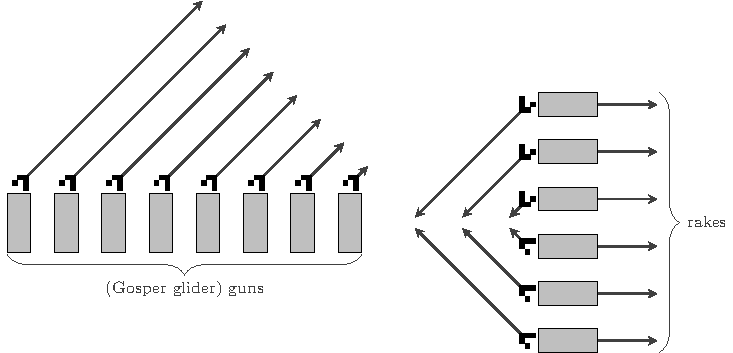
\includegraphics[width=0.9\textwidth]{periodic_circuitry/breeder_schematic.pdf}
		\captionof{figure}{A schematic that gives a rough picture of how the breeder that we constructed in Section~\ref{sec:gosper_breeder} works.}\label{fig:ggg_breeder_schematic}\bigskip
	\end{minipage}
	
	\item[2)] Next, we fill in the details---we place guns, rakes, reflectors, and other components that actually make the gliders (and potentially other spaceships) follow the tracks indicated and perform the required syntheses. For example, when constructing the breeder in Section~\ref{sec:gosper_breeder}, we arranged a total of $12$ period~$60$ space rakes at the right-hand-side of the pattern to carry out the indicated Gosper glider gun synthesis.\smallskip
\end{enumerate}

Depending on the complexity of the schematic, implementing the second step above might be rather tricky, as manipulating glider paths and timing can be a somewhat fiddly and time-consuming affair. In this chapter, our goal is to develop circuitry that can help us do exactly this---our goal is to be able to move gliders (and other spaceships) around tracks in such a way that we can make them appear wherever we want, whenever we want.

For now, we focus on periodic circuitry based on oscillators. The advantage of this type of circuitry is that it is typically smaller and simpler than stationary circuitry (which we explore in the next chapter and is based on still lifes). However, it has the disadvantage that it can be difficult or impossible to make circuitry based on different periods work together. For example, if a period-$5$ oscillator is used to reflect a glider in some part of a mechanism, then the glider stream we are working with must have a period that is a multiple of $5$, and all other connected circuitry must also work at the same period.


%%%%%%%%%%%%%%%%%%%%%%%%%%%%%%%%%%%%%%%%%%%%%%%%%%%%%%%%%%%%%%%%%%%%%%%%%
%%   SUBSECTION: P30 CIRCUITRY
%%%%%%%%%%%%%%%%%%%%%%%%%%%%%%%%%%%%%%%%%%%%%%%%%%%%%%%%%%%%%%%%%%%%%%%%%
\section{Period~30 Circuitry}\label{sec:p30}

\begin{wrapfigure}{R}{0.28\textwidth}
	\centering\vspace*{-0.8cm}
	\patternimg{0.125}{buckaroo_reflect}
	\caption{A buckaroo can reflect a glider by $90$~degrees, from the position marked in \bgbox{greenback}{green} to the one in \bgbox{orangeback}{orange} $30$ generations later.}\label{fig:buckaroo_reflect}
\end{wrapfigure}
The simplest set of circuitry that exists is based off of the queen bee shuttle and thus has period~$30$. For example, we already saw that we can use the queen bee shuttle to construct the Gosper glider gun (Figure~\ref{fig:gosper_glider_gun}) and buckaroo (Figures~\ref{fig:buckaroo} and~\ref{fig:buckaroo_reflect}), which create and reflect gliders, respectively. We now present some other oscillators and circuits with compatible periods that can be used in conjunction with period~$30$ glider streams, and we also investigate how we can use these objects to manipulate glider streams in even more exotic ways.


%%%%%%%%%%%%%%%%%%%%%%%%%%%%%%%%%%%%%%%%%%%%%%%%%%%%%%%%%%%%%%%%%%%%%%%%%
%%   SUBSECTION: P30 REFLECTION
%%%%%%%%%%%%%%%%%%%%%%%%%%%%%%%%%%%%%%%%%%%%%%%%%%%%%%%%%%%%%%%%%%%%%%%%%
\subsection{Reflectors}\label{sec:p30_reflectors}

Because the period of the pentadecathlon\index{pentadecathlon} is $15$, which evenly divides $30$, it works very well with other period~$30$ circuitry. In particular, it can be used to reflect gliders in numerous different ways that are shown in Figure~\ref{fig:p30_reflectors}. The reflection shown in Figure~\ref{fig:p30_relay} is the same one that we saw back in the period~$60$ oscillator of Figure~\ref{fig:relay}, but the other two are new.

\begin{figure}[!htb]
	\centering
	\begin{tabular}{ccc}
		\begin{subfigure}{.31\textwidth}
			\centering\vspace*{1.7cm}
			\patternimg{0.1}{p30_relay}
			\caption{A pentadecathlon reflecting by $180$~degrees.}
			\label{fig:p30_relay}
		\end{subfigure} &
		\begin{subfigure}{.31\textwidth}
			\centering\vspace*{0.23cm}
			\patternimglink{0.1}{p30_180_reflect}
			\caption{Two pentadecathlons reflecting by $180$~degrees.}
			\label{fig:p30_180_reflect}
		\end{subfigure} &
		\begin{subfigure}{.31\textwidth}
			\centering
			\patternimglink{0.1}{p30_90_reflect_penta}
			\caption{Two pentadecathlons reflecting by $90$~degrees.}
			\label{fig:p30_90_reflect_penta}
		\end{subfigure}
	\end{tabular}
	\caption{Some period~$15$ pentadecathlon-based reflectors that work well with glider streams whose period is a multiple of~$15$ (the reflector (c) requires period at least~$45$). Input gliders are \bgbox{greenback}{green}, while the location where they will be $30$ generations later is displayed in \bgbox{orangeback}{orange}.}
	\label{fig:p30_reflectors}
\end{figure}

In particular, Figure~\ref{fig:p30_180_reflect} shows how two pentadecathlons can be used as a $180$-degree reflector with slightly different timing and positioning than the one that we already knew about (i.e., the one in Figure~\ref{fig:p30_relay}), and Figure~\ref{fig:p30_90_reflect_penta} shows that two pentadecathlons can be used to create a $90$-degree color-preserving reflector. There are also a few other period~$30$-friendly ways to reflect gliders aside from using pentadecathlons and buckaroos. We will see some color-changing $90$-degree methods in Figures~\ref{fig:p15_bouncer} and~\ref{fig:p5_bouncer}, and two more color-preserving $90$-degree options in Exercises~\ref{exer:bumper_high_period}c and~\ref{exer:bumper_high_period}d.\footnote{It is also trivially the case that stable reflectors work with glider streams whose period is a large enough multiple of~$30$ (at least~$60$ in the case of the Snark).} 


%%%%%%%%%%%%%%%%%%%%%%%%%%%%%%%%%%%%%%%%%%%%%%%%%%%%%%%%%%%%%%%%%%%%%%%%%
%%   SUBSECTION: P30 INVERSION
%%%%%%%%%%%%%%%%%%%%%%%%%%%%%%%%%%%%%%%%%%%%%%%%%%%%%%%%%%%%%%%%%%%%%%%%%
\subsection{The Inline Inverter}\label{sec:p30_inline_inverter}

One of the most useful features of the Gosper glider gun is that it can be turned into an \emph{inline inverter}\index{inline inverter}---a reaction that ``flips'' a period~$30$ glider stream so that any glider present in the stream is destroyed, while any glider missing from the stream is inserted.\footnote{The inline inverter was discovered by David Bell.} The resulting stream travels in the same direction as the input stream, but is slightly offset (see Figure~\ref{fig:inline_inverter}).

The inline inverter provides us with a simple way to construct irregular glider streams. For example, if we feed a period~$120$ glider stream into it, we get as output a period~$30$ glider stream in which only $3$ out of every $4$ gliders are present (see Figure~\ref{fig:inline_inverter_p120}).

\begin{figure}[!htb]
	\centering
	\begin{tabular}{ccc}
		\begin{subfigure}{.45\textwidth}
			\centering
			\patternimglink{0.1}{inline_inverter}
			\caption{inline inverter}
			\label{fig:inline_inverter}
		\end{subfigure} &
		\begin{subfigure}{.51\textwidth}
			\centering
			\patternimglink{0.089}{inline_inverter_p120}
			\caption{inverting a p$120$ stream}
			\label{fig:inline_inverter_p120}
		\end{subfigure}	
	\end{tabular}
	\caption{The inline inverter is a reaction involving the Gosper glider gun in which the gun fails to produce a glider if it receives a glider as input at the same time. (a) If an input glider is \emph{not} present then an output glider will appear at the location marked in \bgbox{greenback}{green} $30$ generations after the phase shown here (i.e., the output stream is $5$ cell further south than the input stream). (b) An inline inverter can be used to turn thin glider stream into a thick one (in this case, a period~$120$ glider stream into a period~$30$ stream that is missing one out of every four gliders).}
	\label{fig:inline_inverter_both}
\end{figure}

Similarly, we can use one Gosper glider gun to feed gliders into an inline inverter, creating a period~$30$ oscillator made up of a glider stream of any finite length of our choosing. We could of course do the same thing simply by aiming the glider stream from a Gosper glider gun at an eater (as in Exercise~\ref{exer:gosper_oscillator}), but this method has the advantage that we can trigger it to release a glider by destroying one of the gliders in the middle stream. For example, we can use one of the two-glider collisions from Table~\ref{tab:2_glider_synth} to have a glider bounce off of the glider stream, resulting in a single other glider escaping from the stream, as in Figure~\ref{fig:inline_inverter_bounce}.

\begin{figure}[!htb]
	\centering
	\embedlink{inline_inverter_bounce}{\vcenteredhbox{\patternimg{0.116}{inline_inverter_bounce}} \vcenteredhbox{\genarrow{15}} \vcenteredhbox{\patternimg{0.116}{inline_inverter_bounce_15}} \vcenteredhbox{\genarrow{15}} \vcenteredhbox{\patternimg{0.116}{inline_inverter_bounce_30}}}
	\caption{Two Gosper glider guns can be placed near each other so as to create a finite stream of gliders (shown here in \bgbox{aquaback}{aqua}) between them. Here, we bounce a single glider (in \bgbox{greenpastel}{green}) off of one of those gliders (in \bgbox{magentaback}{magenta}) so that it is destroyed and thus released by the inline inverter to the southeast.}
	\label{fig:inline_inverter_bounce}
\end{figure}

By bouncing a glider back and forth between two of these finite-length glider streams, we can create glider guns with arbitrarily large periods. In particular, by shifting these two mechanisms $15$ cells farther away from each other, we can create glider guns with period equal to $120n$ for any integer $n \geq 1$. Figure~\ref{fig:inline_inverter_p120_gun} illustrates a gun of this type of period~$120$.

We should clarify at this point that there are actually many other methods of stream inversion possible as well, but the inverted stream is typically reflected by $90$~degrees from the input stream, rather than going in the same direction as it (i.e., the inversion is not ``inline'').\footnote{We will see a period~$46$ inline inverter a bit later in this chapter, in Figure~\ref{fig:tanners_p46_inline_inverter}.} For example, simply firing an irregular stream at a regular stream so that they collide as in one of the two-glider annihilations from Table~\ref{tab:2_glider_synth} gives an inverter. This inverter can do many of the same things as the inline inverter, such as creating high-period guns as in Figure~\ref{fig:inverter_p120_gun}. If desired, we can turn this inversion into one that is inline simply by pairing it with any compatible 90-degree periodic reflector, or with a Snark as long as the period is $43$ or greater.

\begin{figure}[!htb]
	\centering
	\begin{subfigure}{.46\textwidth}
		\centering
		\patternimglink{0.075}{inline_inverter_p120_gun}
		\caption{p$120$ gun from inline inverter}
		\label{fig:inline_inverter_p120_gun}
	\end{subfigure} \ \ % 
	\begin{subfigure}{.5\textwidth}
		\centering
		\patternimglink{0.075}{inverter_p120_gun}
		\caption{p$120$ gun from collision-based non-inline inverter}
		\label{fig:inverter_p120_gun}
	\end{subfigure}
	\caption{Three Gosper glider guns (highlighted in \bgbox{yellowback2}{yellow}, the bottom of which acts as an inverter) can be used to create a period~$120$ glider gun. The glider outlined in \bgbox{greenpastel}{green} bounces back and forth between the two \bgbox{aquaback}{aqua} glider streams, destroying one glider in each stream every time it is reflected. The glider that is destroyed in the left stream is then created (in \bgbox{magentaback}{magenta}) by the inverter. In (a), the bottom glider gun is an inline inverter whereas it is a non-inline inverter in (b). The period of these guns can be increased by~$120$ generations by moving the top-right glider gun and eater northeast by $15$ cells.}\label{fig:inverter_p120_gun_inline_and_not}
\end{figure}

Another slightly more useful (non-inline) inversion reaction is provided in Figure~\ref{fig:stream_inverter}, in which a glider stream of any period $20$ or larger comes in from the northwest, and a stream of the same period (but potentially with some gliders missing) comes in from the northeast. When the stream from the northwest reaches the block, it either passes by unharmed (if there is no corresponding glider in the stream from the northeast), or it collides with the glider from the northeast, producing a single glider to the southwest. Thus two output glider streams are produced: one to the southwest that contains the same gliders and spacing as the northeast input stream (which can be destroyed with an eater if it is not needed), and one to the southeast that is the inverse of the northeast input stream.

\begin{figure}[!htb]
	\centering
	\begin{subfigure}{.48\textwidth}
		\centering
		\embedlink{stream_inverter}{\vcenteredhbox{\patternimg{0.1}{inverter0_0}} \vcenteredhbox{\genarrow{12}} \vcenteredhbox{\patternimg{0.1}{inverter0_12}}}
		\caption{This collision causes the top-right glider to be erased and the top-left glider to be slightly offset.}
		\label{fig:stream_inverter_yes}
	\end{subfigure} \ \ \ \ % 
	\begin{subfigure}{.48\textwidth}
		\centering
		\embedlink{stream_inverter}{\vcenteredhbox{\patternimg{0.1}{inverter1_0}} \vcenteredhbox{\genarrow{12}} \vcenteredhbox{\patternimg{0.1}{inverter1_12}}}
		\caption{If the top-left glider is omitted, the top-right glider passes by unharmed.}
		\label{fig:stream_inverter_no}
	\end{subfigure}
	\caption{A stream inverter that splits the glider stream coming in from the northeast based on which gliders are present in the stream coming in from the northwest. This reaction can be used with any glider stream of period~$20$ or higher.}\label{fig:stream_inverter}
\end{figure}

By reflecting the inverted stream and using an eater to destroy the other output stream, we can use this reaction to create an inline inverter of any period at least $20$ (as long as the repeat time of the reflector is low enough---see Exercise~\ref{exer:make_inline_inverter_with_weird_period}). Even more remarkably, we can combine this reaction with another inverter to duplicate arbitrary glider streams (even irregular ones with holes), simply by inverting the inverted output stream, as in Figure~\ref{fig:glider_duplicator}. Patterns like this one are called \emph{glider duplicators}\index{glider duplicator}, and they are extremely important because they let us use a single input signal (i.e., a glider) to trigger multiple different reactions.

\begin{figure}[!htb]
	\centering
	\embedlink{glider_duplicator}{\vcenteredhbox{\patternimg{0.1}{glider_duplicator_0}} \vcenteredhbox{\genarrow{30}} \vcenteredhbox{\patternimg{0.1}{glider_duplicator_30}} \vcenteredhbox{\genarrow{60}} \vcenteredhbox{\patternimg{0.1}{glider_duplicator_90}}}
	\caption{A glider duplicator that makes use of the inline inverter and the reaction from Figure~\ref{fig:stream_inverter}. The input glider from the northwest (highlighted in \bgbox{aquaback}{aqua}) is copied to the southeast and destroys the corresponding glider going southwest. The southern inline inverter then creates a glider going southwest, thus duplicating the original glider.}\label{fig:glider_duplicator}
\end{figure}


\subsection{Miscellaneous Period~30 Circuits}\label{sec:p30_misc_circuits}

There are also a few other useful tricks that can be done with period~$30$ glider streams in order to make them easier to work with. For example, one object that can be used to help push glider streams closer together (which is extremely useful when trying to implement some tight glider syntheses) is a \emph{glider pusher}\index{glider pusher},\footnote{Found by Dietrich Leithner in December 1993.} which is a combination of a (half-stabilized) queen bee and a pentadecathlon that push a glider over by a single lane (see Figure~\ref{fig:glider_pusher_main}).\footnote{We first saw this glider pusher in Exercise~\ref{exer:hwss_gun}b.}

Two other simple reactions that make use of the debris and sparks left behind by queen bees and pentadecathlons are shown in Figures~\ref{fig:glider_to_lwss} and~\ref{fig:lwss_to_glider}. These reactions let us convert gliders directly into lightweight spaceships (rather than having to synthesize them via $3$ gliders) and then convert them back into gliders if desired. Note, however, that the former reaction can only be used with streams of period at least~$60$, since otherwise the output LWSS collides with the next input glider.

\begin{figure}
	\centering
	\begin{minipage}{0.31\textwidth}
		\centering
		\patternimglink{0.075}{glider_pusher}
		\caption{A \emph{glider pusher} pushes a glider away by one lane.}\label{fig:glider_pusher_main}
	\end{minipage}\quad
	\begin{minipage}{0.31\textwidth}
		\centering\vspace*{1.13cm}
		\patternimglink{0.105}{glider_to_lwss}
		\caption{Two queen bees can convert a glider into an LWSS.}\label{fig:glider_to_lwss}
	\end{minipage}\quad
	\begin{minipage}{0.31\textwidth}
		\centering\vspace*{0.58cm}
		\patternimglink{0.1}{lwss_to_glider}
		\caption{Pentadecathlons can convert an LWSS into a glider.}\label{fig:lwss_to_glider}
	\end{minipage}
\end{figure}

It is worth comparing the the LWSS-to-glider converter of Figure~\ref{fig:lwss_to_glider} to the pentadecathlon-based reflectors of Figures~\ref{fig:p30_180_reflect} and~\ref{fig:p30_90_reflect_penta}. In all three cases, the reaction is made up of two pentadecathlons, the first of which converts the input object (either an LWSS or a glider) into a block and the second of which converts that block into the output glider.

One final piece of machinery that is a bit more heavy-duty than the other period~$30$ reactions that we have illustrated is the \emph{toggle}\index{toggle},\footnote{Found by Dean Hickerson in April 1996.} which is a glider gun that can be switched on and off by firing a single glider into it (contrast this with the inline inverter, which is a glider gun that can be toggled on and off by firing a \emph{constant stream} of gliders into it). The toggle works by exploiting the fact that a glider can strike a particular phase of an LWSS in a way that destroys the LWSS and creates a perpendicular output glider---but if the incoming glider is delayed by $30$~generations then both are simply destroyed.

\begin{figure}[!htb]
	\centering
	\patternimglink{0.12}{toggle}
	\caption{A \emph{toggle} that bounces gliders from a Gosper glider gun (highlighted in \bgbox{yellowback2}{yellow}) off of a stream of lightweight spaceships (highlighted in \bgbox{aquaback}{aqua}). The first incoming glider (on the \bgbox{magentaback}{magenta} stream) turns off the output stream of gliders (highlighted in \bgbox{greenpastel}{green}) until another glider comes in behind it to turn the stream back on.}
	\label{fig:toggle}
\end{figure}


\section{Primer}\label{sec:primer}

We now have enough circuitry and tools at our disposal that we can start to construct some really unusual and interesting patterns. To illustrate how to put these pieces together in non-trivial ways, we now construct a pattern that computes prime numbers.\index{prime number} More specifically, we build a pattern that emits a stream of lightweight spaceships with the property that the $n$-th spaceship in the stream is present if and only if $n$ is prime. That is, we construct a pattern that emits a stream of lightweight spaceships with spacing as in Figure~\ref{fig:prime_lwss_stream}. We call patterns of this type \emph{primers}.\index{primer}\footnote{The first primer was constructed by Dean Hickerson in November 1991. It used the same techniques that we will demonstrate here, but some of the component reactions were slightly different (e.g., instead of the inline inverter, it used a stream inversion reaction that we will see in Section~\ref{sec:stream_inversion}).}

\begin{figure}[!ht]
	\centering\begin{tikzpicture}[scale=0.9, every node/.style={transform shape}]%
		\node[inner sep=0pt,anchor=south west] at (0,0) {\patternimglink{0.1}{prime_lwss_stream}};
	
		\sizecolorletternode{gray}{0.72}{0.57}{1}{9.5}
		\sizecolorletternode{green}{1.57}{0.57}{2}{9.5}
		\sizecolorletternode{green}{2.42}{0.57}{3}{9.5}
		\sizecolorletternode{gray}{3.26}{0.57}{4}{9.5}
		\sizecolorletternode{green}{4.11}{0.57}{5}{9.5}
		\sizecolorletternode{gray}{4.96}{0.57}{6}{9.5}
		\sizecolorletternode{green}{5.81}{0.57}{7}{9.5}
		\sizecolorletternode{gray}{6.66}{0.57}{8}{9.5}
		\sizecolorletternode{gray}{7.51}{0.57}{9}{9.5}
		\sizecolorletternode{gray}{8.31}{0.57}{10}{9.5}
		\sizecolorletternode{green}{9.18}{0.57}{11}{9.5}
		\sizecolorletternode{gray}{10.01}{0.57}{12}{9.5}
		\sizecolorletternode{green}{10.86}{0.57}{13}{9.5}
		\sizecolorletternode{gray}{11.71}{0.57}{14}{9.5}
		\sizecolorletternode{gray}{12.56}{0.57}{15}{9.5}
		\sizecolorletternode{gray}{13.41}{0.57}{16}{9.5}
		\sizecolorletternode{green}{14.25}{0.57}{17}{9.5}
		\sizecolorletternode{gray}{15.1}{0.57}{18}{9.5}
		\sizecolorletternode{green}{15.95}{0.57}{19}{9.5}
	\end{tikzpicture}
	\caption{A stream of lightweight spaceships in which only the prime-indexed spaceships are present.}\label{fig:prime_lwss_stream}
\end{figure}


\subsection{A LWSS Gun with an Irregular Stream}\label{sec:primer_irregular_stream}

Before building the desired primer itself, let's start by constructing a (much simpler) pattern that emits a stream of lightweight spaceships with the property that the $n$-th spaceship in the stream is present if and only if $n$ is not a multiple of $2$ or $3$. Since we do not have any methods
\begin{wrapfigure}{r}{0.28\textwidth}
	\centering
	\embedlink{glider_lwss_destroy}{\vcenteredhbox{\patternimg{0.12}{glider_lwss_destroy}} \vcenteredhbox{\genarrow{8}} \vcenteredhbox{\patternimg{0.12}{glider_lwss_destroy_8}}}
	\caption{A glider and an LWSS destroying each other.}\label{fig:glider_lwss_destroy}
\end{wrapfigure}
for creating streams of spaceships with irregular spacing directly, we will instead create a stream of lightweight spaceships and strategically destroy the unwanted spaceships in it (i.e., we destroy all lightweight spaceships corresponding to multiples of $2$ or multiples of $3$). Figure~\ref{fig:glider_lwss_destroy} shows how we can fire a glider at a lightweight spaceship so as to destroy them both.\footnote{Reactions like this one, where two small objects are used to destroy each other, can easily be found by hand. Just try a few collisions with slightly different positioning and timing, and one of them will likely work.} Thanks to this reaction, we can create the desired stream of lightweight spaceships simply by aiming two glider guns at a stream of lightweight spaceships: one with double the period of the LWSS stream (to eliminate the multiples of $2$) and one with triple its period (to eliminate the multiples of $3$). A schematic for such a pattern is presented in Figure~\ref{fig:period_not_2_3_lwss_gun_schematic}. 

\begin{figure}[!htb]
	\centering
	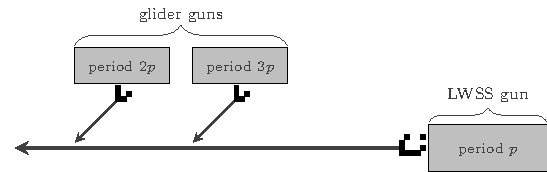
\includegraphics[width=0.6\textwidth]{periodic_circuitry/period_not_2_3_lwss_gun_schematic.pdf}
	\caption{A schematic for a LWSS gun that fires an irregular stream of spaceships with the property that the $n$-th spaceship in the stream is present if and only if $n$ is not a multiple of $2$ or $3$. Gliders are used to delete every second and every third spaceship in the LWSS stream.}
	\label{fig:period_not_2_3_lwss_gun_schematic}
\end{figure}

To actually construct such a pattern, we make use of the period~$30$ circuitry that we have seen so far. If the period of the LWSS gun that we use is $p$, then we need glider guns with periods~$2p$ and~$3p$ as well. Since we do not yet know how to construct guns with periods~$60$ or~$90$ (we will learn how to do so in Section~\ref{sec:glider_deletion}), it seems natural to use the period~$120n$ guns based on the inline inverter that we introduced in Figure~\ref{fig:inline_inverter_p120_gun}. In particular, we arrange three period~$120$ guns so as to synthesize the LWSS and then aim period~$240$ and~$360$ guns at the resulting LWSS stream in order to thin it out. The final pattern is displayed in Figure~\ref{fig:period_not_2_3_lwss_gun}.

\begin{figure}[!htb]
	\centering
	\patternimglink{0.111}{period_not_2_3_lwss_gun}
	\caption{A gun that shoots an irregularly-spaced stream of lightweight spaceships. In particular, the period~$120$ inline inverter gun makes use of the glider-to-LWSS reaction from Figure~\ref{fig:glider_to_lwss} (highlighted in \bgbox{greenpastel}{green}) to create a period~$120$ stream of lightweight spaceships (highlighted in \bgbox{magentaback}{magenta}). Period~$240$ and period~$360$ inline inverter guns (highlighted in \bgbox{yellowback2}{yellow} and \bgbox{aquaback}{aqua}, respectively) then destroy every LWSS with a position in the stream that is a multiple of $2$ or $3$, respectively.}
	\label{fig:period_not_2_3_lwss_gun}
\end{figure}


\subsection{The Prime-Generating Gun Itself}\label{sec:primer_itself}

The gun that we just constructed contains the key idea used in our prime-generating gun---we create a period~$p$ ($p = 120$) stream of lightweight spaceships and then aim glider guns with periods~$2p$, $3p$, $4p$, $5p$, and so on at the gun to delete any lightweight spaceships whose position in the stream is a multiple of $2$, $3$, $4$, $5$, $\ldots$, respectively.

The tricky part is that we now have to find a way to construct infinitely many glider guns (like the breeder) with ever-increasing periods (\emph{unlike} the breeder). Fortunately, the period~$120n$ guns based on the inline inverter are perfect candidates for this task, since their periods are determined solely by how far apart the two Gosper glider guns at their ends are. Thus one way to construct glider guns with ever-increasing periods is to send one set of rakes north to synthesize Gosper glider guns and another set of rakes east to do the same. The diagonal distance (along which a single glider will travel) between these endpoint Gosper glider guns will increase without bound, giving us glider guns of larger and larger periods. We thus arrive at the schematic presented in Figure~\ref{fig:primer_schematic} for synthesizing these high-period glider guns and thus our primer.

\begin{figure}[!htb]
	\centering
	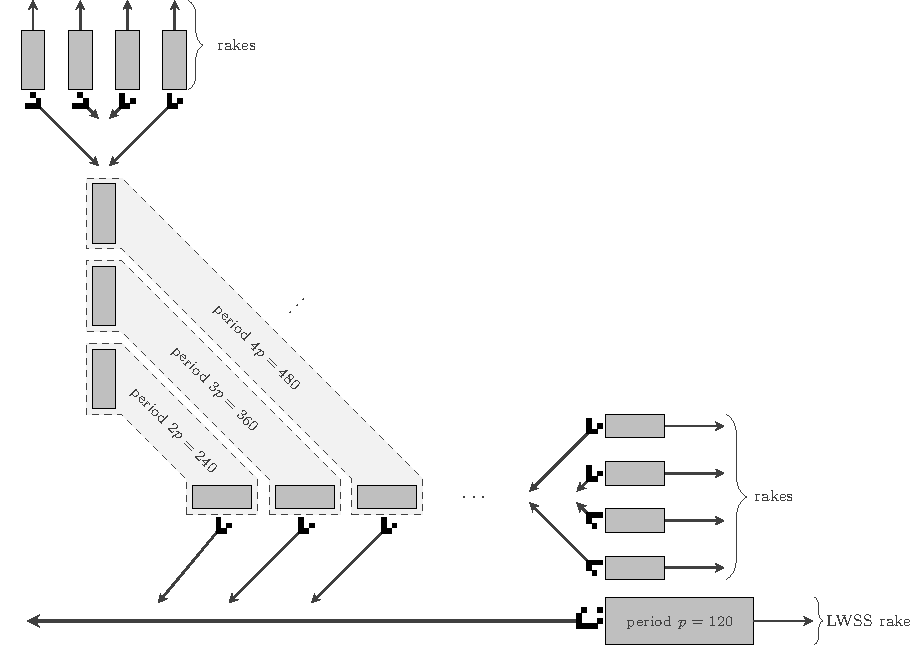
\includegraphics[width=\textwidth]{periodic_circuitry/primer_schematic.pdf}
	\caption{A schematic for a primer. For each integer $n \geq 2$, eastward and northward sets of rakes leave behind halves of the period~$120n$ glider gun based on the inline inverter, which is used to destroy every LWSS in the bottom period~$120$ stream whose position is a multiple of $n$. The only spaceships that escape to the far left are the ones whose position is not evenly divisible by any smaller integer $n \geq 2$ (i.e., the primes).}
	\label{fig:primer_schematic}
\end{figure}

This is by far our biggest construction to date---the breeder from Section~\ref{sec:gosper_breeder} was already quite large, and it just laid one row of Gosper glider guns, while this construction requires us to lay \emph{three} rows of Gosper glider guns (two going eastward and one going northward). It is thus worthwhile to present a more compact Gosper glider gun breeder that we can use as a component in our primer---see Figure~\ref{fig:breeder_compact}. Although this breeder looks quite different from our original one of the surface, it functions in more or less the same way by making use of several period~$60$ space rakes to gradually build the Gosper glider guns up piece-by-piece.

\begin{figure}[!htb]
	\centering
	\embedlink{breeder_compact}{\vcenteredhbox{\patternimg{0.123}{breeder_compact}} \vcenteredhbox{\genarrow{360}} \vcenteredhbox{\patternimg{0.123}{breeder_compact_360}}}
	\caption{A compact breeder that uses $6$ period~$60$ space rakes to carry out an incremental synthesis of a Gosper glider gun. It gets away with fewer space rakes than our original breeder from Figure~\ref{fig:breeder_done} (which used $12$) since it cleverly manipulates the debris behind the two frontmost space rakes to create a ship, which is the most difficult part of the Gosper glider gun's incremental synthesis to create.}
	\label{fig:breeder_compact}
\end{figure}

Unfortunately, there are actually quite a few subtle problems with the previous schematic that prevent us from building it as-is:\smallskip

\begin{enumerate}
	\item[1)] The only Gosper glider gun breeder that we know how to build so far has period~$60$, which results in Gosper glider guns that are separated by $30$~cells and thus inline inverter guns with periods that increase by $240$ (not $120$).
	
	In order to solve this problem, our first instinct might be to create a period~$240$ stream of lightweight spaceships instead of a period~$120$ stream. However, since we do not yet know how to do this, we instead use the breeders to create glider guns with periods~$3p$, $5p$, $7p$, $9p$, $\ldots$ to delete any lightweight spaceships whose position in the stream is a multiple of $3$, $5$, $7$, $9$, $\ldots$, respectively, and then manually place a single glider gun of period~$2p$ to delete the leftover lightweight spaceships whose positions in the stream are a multiple of $2$.\smallskip
	
	\item[2)] With the Gosper glider guns just $30$~cells apart, we cannot fire gliders back and forth between them diagonally---the bouncing gliders would collide with the blocks that stabilize the glider guns.
	
	In order to solve this problem, we do the same thing that we did in Figure~\ref{fig:inline_inverter_p120_gun} to squeeze Gosper glider guns closer together---we replace one of the stabilizing blocks by an eater~1 (as in the buckaroo of Figure~\ref{fig:buckaroo_reflect}). To create a row of these modified Gosper glider guns, we can use the breeder in Figure~\ref{fig:breeder_ggg_eater_1_stabilize}, which is just a slight modification of the breeders that we have already seen.\footnote{We already constructed a (much larger) breeder for this modification of the Gosper glider gun back in Exercise~\ref{exer:ggg_eater_side_breeder}.}\bigskip
	
	\noindent\begin{minipage}{\linewidth}
		\centering
		\patternimglink{0.089}{breeder_ggg_eater_1_stabilize}
		\captionof{figure}{A Gosper glider gun breeder that is stabilized on one side by an eater~1 instead of a block. The bottom half (highlighted in \bgbox{greenpastel}{green}) is the same as the bottom half of of the compact breeder from Figure~\ref{fig:breeder_compact}. The bottom-right space rake (highlighted in \bgbox{yellowback2}{yellow}) turns one of the blinkers from the blinker puffer (highlighted in \bgbox{magentaback}{magenta} and introduced in Exercise~\ref{exer:schick_engine_blinker_puffer}) into a ship via the incremental synthesis that we saw in Table~\ref{tab:sequential_synth}. The rightmost space rake (highlighted in \bgbox{orangeback}{orange}) synthesizes the top ship into a queen bee, while the remaining three space rakes (highlighted in \bgbox{aquaback}{aqua}) synthesize the eater~1.}\label{fig:breeder_ggg_eater_1_stabilize}\bigskip
	\end{minipage}
	
	\item[3)] When constructing the two east--west rows of Gosper glider guns, if their construction is not synchronized perfectly then the bottom row will release some gliders in the time between when it is constructed and when gliders from the top row are fed into it. This problem can be solved by using a fixed-length row of middleweight (or heavyweight) spaceships below those guns to destroy the excess gliders as in Figure~\ref{fig:orthogonal_destroy}.\smallskip
	
	\item[4)] A period $3p$ gun (for example) will erase all lightweight spaceships whose position in the stream is a multiple of $3$, \emph{including $3$ itself}, while we only want it to erase the multiples of $3$ greater than $3$. To solve this final problem, we can place a single block below each inline inverter gun in such a way that it destroys (and is destroyed by) the first glider released from the gun. This row of blocks can simply be synthesized by two space rakes.\smallskip
\end{enumerate}

After putting all of these pieces together, we arrive at our completed primer in Figure~\ref{fig:primer}. We emphasize that static pictures really cannot do this pattern justice, so the reader is strongly encouraged to interact with and explore this pattern in Life-viewing software.

% Footnote above about Golly?

% EXERCISE to add: move stuff at the right to the left a bit to make MWSS line shorter and breeder smaller. Advanced exercise to rewind it as much as possible

\begin{figure}[!htb]
	\centering
	\patternimglink{0.108}{primer}
	\caption{The completed primer. The period~$120$ stream of lightweight spaceships (highlighted in \bgbox{magentaback}{magenta} and synthesized by $3$ space rakes as in Exercise~\ref{exer:p60_lwss_backrake}) moves to the left and is thinned out by the inline inverter guns (highlighted in \bgbox{aquaback}{aqua}). The leftmost inline inverter gun has period~$240$ and has a different shape from the others (which have periods~$360$, $600$, $840$, and in general $360 + 240n$ for $n \geq 0$). The rows of Gosper glider guns are laid by two copies of the compact breeder from Figure~\ref{fig:breeder_compact} (highlighted in \bgbox{greenpastel}{green}) and the row of Gosper glider guns that are stabilized by eater~1s instead of blocks are laid by the breeder that we presented in Figure~\ref{fig:breeder_ggg_eater_1_stabilize} (highlighted in \bgbox{yellowback2}{yellow}). A single space rake going north (also highlighted in \bgbox{yellowback2}{yellow}) produces the gliders that bounce along the long diagonal of the inline inverter guns, and the remaining pairs of space rakes (highlighted in \bgbox{orangeback}{orange}) simply synthesize rows of block and eater~1s.}
	\label{fig:primer}
\end{figure}


\section{Period~46 Circuitry}\label{sec:p46}

Just like we can use the queen bee shuttle and Gosper glider gun as the basis of a set of period~$30$ circuitry, we can also use the twin bees shuttle (Figure~\ref{fig:twin_bees_shuttle}) and the related twin bees gun (Figure~\ref{fig:twin_bees_gun}) to build up a set of period~$46$ circuitry. For example, the twin bees shuttle can be used to reflect gliders (by either 90~degrees or 180~degrees\footnote{The 180~degree reflection takes 92~generations to complete, since the twin bees shuttle first converts the incoming glider into a block and then converts that block into the output glider. It was found by Dean Hickerson.}) and lightweight spaceships, and even convert gliders \emph{into} lightweight spaceships, and vice-versa, as displayed in Figure~\ref{fig:twin_bees_reflect}.

We saw one of these glider reflections way back in Section~\ref{sec:sparkers}---the twin bees shuttle creates a duoplet spark\index{duoplet spark} that does the reflection.\footnote{This reflection is the one highlighted in green in Figure~\ref{fig:twin_bees_reflect_a}.} The other reflections and the glider-to-LWSS-to-glider conversions all make use of the large spark produced by the form of the twin bees shuttle that is stabilized on one side by just a single block.

\begin{figure}[!htb]
	\centering
	\begin{tabular}{ccc}
		\begin{subfigure}{.31\textwidth}
			\centering
			\embedlink{twin_bees_reflect}{\patternimg{0.085}{twin_bees_reflect_a}}
			\caption{three glider reflections}
			\label{fig:twin_bees_reflect_a}
		\end{subfigure} &
		\begin{subfigure}{.31\textwidth}
			\centering
			\embedlink{twin_bees_reflect}{\patternimg{0.085}{twin_bees_reflect_b}}
			\caption{two more reflections}
			\label{fig:twin_bees_reflect_b}
		\end{subfigure} &
		\begin{subfigure}{.31\textwidth}
			\centering
			\embedlink{twin_bees_reflect}{\patternimg{0.085}{twin_bees_reflect_c}}
			\caption{glider $\rightarrow$ LWSS and back}
			\label{fig:twin_bees_reflect_c}
		\end{subfigure}
	\end{tabular}
	\caption{The twin bees shuttle (highlighted in \bgbox{yellowback2}{yellow}) can be used to reflect a glider by 90~degrees in three different ways ((a)~\bgbox{greenpastel}{green}, (a)~\bgbox{magentaback}{magenta}, and (b)~\bgbox{magentaback}{magenta}), reflect a glider by 180~degrees ((a)~\bgbox{aquaback}{aqua}), reflect a lightweight spaceship by 90~degrees ((b)~\bgbox{aquaback}{aqua}), and turn a glider into a lightweight spaceship and back ((c)~\bgbox{magentaback}{magenta} and (c)~\bgbox{aquaback}{aqua}, respectively).}
	\label{fig:twin_bees_reflect}
\end{figure}

One of the advantages of these new reflections over the old reflection based on the duoplet spark is that they happen near the corner of the shuttle, so they can be used to (for example) merge two period~$46$ glider streams into a single period~$23$ stream, as in the period~$23$ glider gun displayed in Figure~\ref{fig:twin_bees_p23_gun}.\footnote{We say that this is a \emph{pseudo}-period~$23$ gun since the gun itself operates at period~$46$. We discuss pseudo-period guns and true-period guns (which oscillate at the same period as the glider streams they produce) in depth in Chapter~\ref{chp:guns}.} Similarly, by making use of the glider-to-LWSS converter we can easily create period~$46$ glider guns without needing to synthesize them via three glider guns (see Figure~\ref{fig:twin_bees_p46_lwss_gun}). We can even use a careful arrangement of two twin bees shuttles to convert a lightweight spaceship into a middleweight one, and thus create small middleweight spaceship guns (see Figure~\ref{fig:twin_bees_lwss_to_mwss} and Exercise~\ref{exer:twin_bees_mwss_gun}).\footnote{By replacing the input LWSS by an MWSS, this LWSS-to-MWSS conversion can also be used to simply reflect a MWSS by 90~degrees.}
 
\begin{figure}[!htb]
	\centering
	\begin{tabular}{ccc}
		\begin{subfigure}{.36\textwidth}
			\centering
			\patternimglink{0.12}{twin_bees_p23_gun}
			\caption{a period~$23$ glider gun}
			\label{fig:twin_bees_p23_gun}
		\end{subfigure} & 
		\begin{subfigure}{.28\textwidth}
			\centering
			\patternimglink{0.129}{twin_bees_p46_lwss_gun}
			\caption{a period~$46$ LWSS gun}
			\label{fig:twin_bees_p46_lwss_gun}
		\end{subfigure} & 
		\begin{subfigure}{.29\textwidth}
			\centering
			\patternimglink{0.132}{twin_bees_lwss_to_mwss}
			\caption{LWSS $\rightarrow$ MWSS}
			\label{fig:twin_bees_lwss_to_mwss}
		\end{subfigure}
	\end{tabular}
	\caption{The various reflection and conversion reactions involving twin bees can be used to create some useful guns. (a) is a period~$23$ glider gun constructed by reflecting one period~$46$ stream into the gaps in another period~$46$ stream, (b) is a lightweight spaceship gun that uses the glider-to-LWSS conversion from Figure~\ref{fig:twin_bees_reflect_c}, and (c) is an LWSS-to-MWSS conversion that (for example) allows for the construction of a small MWSS gun.}
	\label{fig:twin_bees_weird_guns}
\end{figure}

There are also a few other useful reactions involving the twin bees that can do things like emit two side-by-side streams of gliders (guns like this are called \emph{double-barreled guns}\index{double-barreled gun}), and explore some of these reactions in Exercise~\ref{exer:twin_bees_large_spark}.


%%%%%%%%%%%%%%%%%%%%%%%%%%%%%%%%%%%%%%%%%%%%%%%%%%%%%%%%%%%%%%%%%%%%%%%%%
%%   SUBSECTION: TICKER TAPES and MEMORY CELLS
%%%%%%%%%%%%%%%%%%%%%%%%%%%%%%%%%%%%%%%%%%%%%%%%%%%%%%%%%%%%%%%%%%%%%%%%%
\subsection{Ticker Tapes and Memory Cells}\label{sec:p46_ticker_tape}

\begin{wrapfigure}{R}{0.3\textwidth}
	\centering
	\patternimg{0.12}{twin_bees_duplicate_reflector}
	\caption{A twin bees shuttle reflecting and duplicating a glider.}\label{fig:twin_bees_duplicate_reflector}
\end{wrapfigure}
One of the most useful reactions involving a twin bees shuttle that we have not yet seen is the one displayed in Figure~\ref{fig:twin_bees_duplicate_reflector} in which the shuttle reflects a glider by $90$~degrees and simultaneously duplicates it. This is somewhat smaller and simpler than the glider duplicator that we saw earlier in Figure~\ref{fig:glider_duplicator}, but of course it has the disadvantage of only working at period~$46$.

One interesting thing that we can do with a glider duplicator is attach it to a glider loop so as to produce any (finite) irregular sequence of gliders of our choosing, simply by having that sequence of gliders in the loop itself. For example, the pattern displayed in Figure~\ref{fig:ticker_tape_gun} makes use of a loop in which one glider is present, then the next two are missing, then the next three are present, then four are missing, five are present, and six are missing, so as to create a gun that produces lightweight spaceships with that same spacing.\footnote{This gun produces lightweight spaceships via the glider-to-LWSS reaction of Figure~\ref{fig:twin_bees_reflect_c} instead of just gliders themselves just to make it easier to visualize the output.} Thus we can encode any message in binary and create a gun that emits that message if we interpret the presence of a spaceship as a ``1'' and the absence of a spaceship as a ``0''.

\begin{figure}[!htb]
	\centering
	\patternimglink{0.12}{ticker_tape_gun}
	\caption{A gun that produces an irregular lightweight spaceship stream corresponding to the bitstring 100111000011111000000 (i.e., one LWSS present, then two missing, then three present, and so on). This stream (highlighted in \bgbox{magentaback}{magenta}) is produced simply by duplicating the gliders in the loop (highlighted in \bgbox{aquaback}{aqua}) that have this same spacing and then performing a few basic reflections and a glider-to-LWSS conversion via twin bees shuttles (highlighted in \bgbox{yellowback2}{yellow}).}\label{fig:ticker_tape_gun}
\end{figure}

By placing several of these guns (with different sequences of gliders in their glider loops) near each other, we can even create \emph{ticker tape guns}\index{ticker tape gun}, which emit any \emph{visual} message of our choosing, rather than just encoding messages in binary. To do this, we think of lightweight spaceships as pixels, with the presence of a ship being black and the absence of a ship being white. Each of the loop-based guns emits the pixels (ships) in a single row of the image being produced, so we use $n$ of the guns with $m$ gliders each in the loops to create an $n \times m$ image. For example, Figure~\ref{fig:ticker_tape_hi_gun} illustrates a ticker tape gun that repeatedly produces an $8 \times 21$ array of lightweight spaceships that spells out ``HI!''.\footnote{Alan Hensel put together the first ticker tape gun in June 1994, which printed out the digits ``0123456789''. It was adapted by Brice Due and Dave Greene in 2005 and 2006 to print out the Golly logo, and has been used as the header of the Golly homepage (\httpurl{golly.sourceforge.net/}) ever since.}

\begin{figure}[!htb]
	\centering
	\patternimglink{0.095}{ticker_tape_hi_gun}
	\caption{An arrangement of $8$ loop-based guns that produce an array of lightweight spaceships that spell out ``HI!'' (highlighted in \bgbox{magentaback}{magenta}). Each gun produces one row of the output image (highlighted in \bgbox{yellowback2}{yellow}, \bgbox{greenpastel}{green}, and \bgbox{aquaback}{aqua}), and the arrangement of gliders in each loop controls which lightweight spaceships are produced in their row.}\label{fig:ticker_tape_hi_gun}
\end{figure}

Once we start talking about building things like computers in the Game of Life (which we will do in Chapter~\ref{chp:universal_computation}), loops like this will be quite useful since they can serve as pieces of memory for the computer to make use of (for example, the gun in Figure~\ref{fig:ticker_tape_gun} stores the bitstring ``100111000011111000000'', which we can read from memory by detecting the spaceships that are constantly emitted from the gun). To make loops like this truly useful for storing pieces of information though, we need to be able to easily alter the state of the memory (i.e., delete gliders from the loop and also insert new gliders into it).

Deleting a glider from the loop is simple, since we can just fire another glider from elsewhere in the Life plane so as to collide with it, thus deleting them both. Furthermore, if we replace two of the reflectors in the loop with an inverter (such as the one that we used in Figure~\ref{fig:inverter_p120_gun}), we can then insert gliders into the loop simply by deleting gliders from its inverted portion. This completed pattern is called a \emph{memory cell}\index{memory cell}, and it is illustrated in Figure~\ref{fig:p46_memory_cell} along with the mechanisms for altering the contents of its memory.

\begin{figure}[!htb]
	\centering
	\embedlink{p46_memory_cell}{\vcenteredhbox{\patternimg{0.105}{p46_memory_cell_0}} \vcenteredhbox{\genarrow{552}} \vcenteredhbox{\patternimg{0.105}{p46_memory_cell_552}}}
	\caption{A period $12 \times 46 = 552$ memory cell for which the $12$-bit string ``111010111011'' is encoded along its glider loop (highlighted in \bgbox{aquaback}{aqua}) and is thus repeatedly fired out as a stream of lightweight spaceships (highlighted in \bgbox{magentaback}{magenta}). Bits can be switched from $1$ to $0$ (i.e., gliders can be deleted) simply by sending in a glider from the northwest (highlighted in \bgbox{orangeback2}{orange}) to collide with the loop. Since the northeast side of the glider loop is inverted, bits can be switched from $0$ to $1$ (i.e., gliders can be inserted) by similarly sending in a glider from the northeast (highlighted in \bgbox{greenpastel}{green}) to collide with that side of the loop. As shown here, the $8$th and $10$th bits are flipped, thus changing the bitstring in memory to ``1110101\textbf{0}1\textbf{1}11''.}\label{fig:p46_memory_cell}
\end{figure}


%%%%%%%%%%%%%%%%%%%%%%%%%%%%%%%%%%%%%%%%%%%%%%%%%%%%%%%%%%%%%%%%%%%%%%%%%
%%   SUBSECTION: TANNER'S P46
%%%%%%%%%%%%%%%%%%%%%%%%%%%%%%%%%%%%%%%%%%%%%%%%%%%%%%%%%%%%%%%%%%%%%%%%%
\subsection{Tanner's p46}\label{sec:p46_tanner}

One of the most useful tools for extending our period~$46$ toolset beyond just things that can be done with twin bees is an extremely sparky period~$46$ oscillator called \emph{Tanner's p46}\index{Tanner's p46},\footnote{Found by Tanner Jacobi in October 2017.} which is displayed
%\begin{wrapfigure}{r}{0.3\textwidth}
%	\centering
%	\patternimg{0.1}{tanners_p46}
%	\caption{\emph{Tanner's p46} is a very sparky period~$46$ oscillator.}\label{fig:tanners_p46}
%\end{wrapfigure}
in Figure~\ref{fig:tanners_p46}. It works by using some still lifes to hassle and stabilize a pi-heptomino on $3$ of its $4$ sides. In fact, the boat with tail and snake on its southern side are used to rotate the pi-heptomino in the exact same way as in the p$32$ ``gourmet''\index{gourmet} oscillator that we saw back in Figure~\ref{fig:p32_pi_hassler}.

As is typical of extremely sparky oscillators, Tanner's p46 can be combined with other oscillators or additional copies of itself to create numerous useful objects. For example, it can be combined with a single twin bees to create a new p$46$ glider gun (see Exercise~\ref{exer:tanners_p46_twin_bee_gun}), or it can be used to reflect a glider by 180~degrees (see Exercise~\ref{exer:tanners_p46_reflect}), but neither of these facts are too exciting since we already know how to construct p$46$ glider guns and reflectors of roughly the same size via twin bees. However, by carefully placing two copies of itself next to each other, it can be used to construct an \emph{edge-shooting glider gun}\index{edge-shooting gun}\footnote{Found by David Bell just three days after Tanner's p$46$ itself was found.} (see Figure~\ref{fig:tanners_p46_edge}). Edge shooters\index{edge shooter!edge-shooting gun} like this one are particularly useful when trying to line up streams of gliders in tight positions, since they can be positioned as close as we like to glider streams on one side (compare this with guns like the Gosper glider gun and twin bees guns, which produce the stream of gliders near their center and thus require some clearance on either side of the new glider stream).

Furthermore, this glider gun can act as a p$46$ inline inverter (see Figure~\ref{fig:tanners_p46_inline_inverter}) in the exact same way that the Gosper glider gun can act as a p$30$ inline inverter.\footnote{This inline inverter, just like the original p$30$ one, was found by David Bell.} Even more remarkably, two of these oscillators can be placed next to each other so as to create the p$46$ middleweight spaceship gun\footnote{Found by Matthias Merzenich just one day after Tanner's p$46$ was found.} displayed in Figure~\ref{fig:tanners_p46_mwss_gun}, which is currently the smallest known MWSS gun of any period and also the smallest known gliderless gun of any period.

\begin{figure}[!htb]
	\centering
	\begin{tabular}{ccc}
		\begin{subfigure}{.31\textwidth}
			\centering\vspace*{0.32cm}
			\patternimglink{0.08}{tanners_p46_edge}
			\caption{an edge-shooting glider gun}
			\label{fig:tanners_p46_edge}
		\end{subfigure} &
		\begin{subfigure}{.31\textwidth}
			\centering
			\patternimglink{0.08}{tanners_p46_inline_inverter}
			\caption{an inline inverter}
			\label{fig:tanners_p46_inline_inverter}
		\end{subfigure} &
		\begin{subfigure}{.31\textwidth}
			\centering\vspace*{1.0cm}
			\patternimglink{0.08}{tanners_p46_mwss_gun}
			\caption{a small MWSS gun}
			\label{fig:tanners_p46_mwss_gun}
		\end{subfigure}	
	\end{tabular}
	\caption{Two guns formed by placing two copies of Tanner's p$46$ next to each other so that their sparks interact. The glider gun in (a) can be used as an inline inverter, as in (b), where the incoming glider (highlighted in \bgbox{magentaback}{magenta}) prevents a glider from being fired from the gun at that point in the stream. The gun in (c) is the smallest known MWSS gun.}
	\label{fig:tanners_p46_guns}
\end{figure}

As an example of what can be done with the edge-shooting gun of Figure~\ref{fig:tanners_p46_edge}, we note that it can be used to make a heavyweight spaceship gun via the $3$-glider HWSS synthesis that we saw back in Table~\ref{tab:3_glider_synth}, even though this synthesis contains closely-spaced gliders that cannot be placed by the ``usual'' guns that we have seen so far. An example of such a gun is presented in Figure~\ref{fig:p46_hwss_gun}.

\begin{figure}[!htb]
	\centering
	\patternimglink{0.09}{p46_hwss_gun}
	\caption{A period~$46$ heavyweight spaceship gun that uses two copies of the edge shooter from Figure~\ref{fig:tanners_p46_edge} (highlighted in \bgbox{aquaback}{aqua} and \bgbox{magentaback}{magenta}) to place the required gliders in the HWSS synthesis close together.}
	\label{fig:p46_hwss_gun}
\end{figure}


%%%%%%%%%%%%%%%%%%%%%%%%%%%%%%%%%%%%%%%%%%%%%%%%%%%%%%%%%%%%%%%%%%%%%%%%%
%%   SUBSECTION: HEISENBURPS
%%%%%%%%%%%%%%%%%%%%%%%%%%%%%%%%%%%%%%%%%%%%%%%%%%%%%%%%%%%%%%%%%%%%%%%%%
\subsection{Heisenburps}\label{sec:p46_heisenburps}

We saw back in Figure~\ref{fig:glider_duplicator} that it is possible to construct periodic circuits that duplicate gliders, though the timing and positioning of the output gliders typically do not match those of the input glider.\footnote{In fact, we saw that there are \emph{stationary} circuits that duplicate gliders way back in Figure~\ref{fig:894_reflector}, but these circuits are still a bit more mysterious.} We could of course use various other circuits to correct the positioning and timing of one of the output gliders, but remarkably there exist duplicators for which this is not necessary, as the input glider is not actually affected at all (even temporarily) by the duplication process.

Duplicators of this type are called \emph{Heisenburps}\index{Heisenburp}\footnote{Named for Heisenburg's uncertainty principle, which says that it is impossible to detect a particle without affecting it in some way. Heisenburps show that this principle does \emph{not} hold in Conway's Game of Life, since we can detect and duplicate a particle (glider) without affecting it at all.}, and by far the simplest one known\footnote{Found by Brice Due in January 2005.} is displayed in Figure~\ref{fig:p46_natural_heisenburp}. In this configuration, the spark from two perpendicular twin bees is suppressed slightly by a passing glider so that instead of dying off, the spark turns into another glider. Importantly, the passing glider itself is not affected at all in the process, but rather just serves to overpopulate other nearby cells (much like how we used induction coils to overpopulate and stabilize objects in Section~\ref{sec:still_life_grammar}).

\begin{figure}[!htb]
	\centering
	\embedlink{p46_natural_heisenburp}{\vcenteredhbox{\patternimg{0.12}{p46_natural_heisenburp_0}} \vcenteredhbox{\genarrow{46}} \vcenteredhbox{\patternimg{0.12}{p46_natural_heisenburp_46}} \vcenteredhbox{\genarrow{46}} \vcenteredhbox{\patternimg{0.12}{p46_natural_heisenburp_92}}}
	\caption{A small period~$92$ Heisenburp that uses two twin bees shuttles (highlighted in \bgbox{yellowback2}{yellow}) to copy a glider (highlighted in \bgbox{aquaback}{aqua}) without affecting it. The first $46$ generations are used to create a block (highlighted in \bgbox{magentaback}{magenta}) from the glider and the twin bees spark and the next $46$ generations are used to turn the block into another glider.}\label{fig:p46_natural_heisenburp}
\end{figure}

Heisenburps can also copy other spaceships or even use one type of passing spaceship to create a completely different kind of object---all that is needed is a spark whose evolution is changed sufficiently by the passing spaceship that it turns into something that moves out of the way. For example, the configuration of two twin bees shuttles in Figure~\ref{fig:mwss_out_of_the_blue}, called the \emph{MWSS out of the blue}\index{MWSS out of the blue},\footnote{Found by Peter Rott in November 1997.} detects a passing lightweight spaceship and releasing a middleweight spaceship traveling in the opposite direction in response.

\begin{figure}[!htb]
	\centering
	\embedlink{mwss_out_of_the_blue}{\vcenteredhbox{\patternimg{0.1}{mwss_out_of_the_blue_0}} \vcenteredhbox{\genarrow{46}} \vcenteredhbox{\patternimg{0.1}{mwss_out_of_the_blue_46}}}
	\caption{The \emph{MWSS out of the blue} is a reaction in which two twin bees shuttles are triggered to create a middleweight spaceship when a lightweight spaceship passes by. The LWSS is not affected at all by the reaction.}\label{fig:mwss_out_of_the_blue}
\end{figure}

There are also some reactions that can be used to \emph{construct} Heisenburps via other periodic circuitry that we have already seen. One of the simplest such reactions is the one displayed in Figure~\ref{fig:heisenburp_reaction_p35}, in which a middleweight and heavyweight spaceship collide with a glider in such a way that if another passing glider is present, then the three colliding spaceships cleanly destroy each other, but if that passing glider is absent then they produce a single glider. This reaction has a repeat time of $35$~generations and thus can be used to construct Heisenburps of any period~$35$ or greater.\footnote{Found by Jason Summers in June 1999, as was the first period~$46$ Heisenburp based on it.}

\begin{figure}[!htb]
	\centering
	\begin{subfigure}{.48\textwidth}
		\centering
		\embedlink{heisenburp_reaction_p35}{\vcenteredhbox{\patternimg{0.1}{heisenburp_reaction_p35_0_0}} \vcenteredhbox{\genarrow{19}} \vcenteredhbox{\patternimg{0.1}{heisenburp_reaction_p35_0_19}}}
		\caption{Mutual annihilation if a nearby glider is present.}
		\label{fig:heisenburp_reaction_p35_0}
	\end{subfigure} \ \ \ \ % 
	\begin{subfigure}{.48\textwidth}
		\centering
		\embedlink{heisenburp_reaction_p35}{\vcenteredhbox{\patternimg{0.1}{heisenburp_reaction_p35_1_0}} \vcenteredhbox{\genarrow{19}} \vcenteredhbox{\patternimg{0.1}{heisenburp_reaction_p35_1_19}}}
		\caption{A single glider is produced if no nearby glider is present.}
		\label{fig:heisenburp_reaction_p35_1}
	\end{subfigure}
	\caption{A collision of a glider, lightweight spaceship, and heavyweight spaceship (highlighted in \bgbox{yellowback2}{yellow}) that results in (a) nothing if there is a nearby passing glider (highlighted in \bgbox{aquaback}{aqua}), and (b) a single glider (highlighted in \bgbox{magentaback}{magenta}) if there is not a nearby passing glider. Since the passing glider is unaffected by the collision, this reaction can be used as a basis for a Heisenburp.}\label{fig:heisenburp_reaction_p35}
\end{figure}

To actually construct a Heisenburp from this reaction, we just combine reactions that we saw earlier---we know how to create streams of gliders, middleweight spaceships, and heavyweight spaceships, so we have no problem creating the three objects needed to fuel the reaction, and then we can just use the stream inverter of our choice to ``fix'' the duplicated output stream (since the reaction creates a glider if and only if an input glider is \emph{not} present, which is the opposite of what we want). Figure~\ref{fig:p46_heisenburp_constructed} demonstrates one way to put these pieces together using period~$46$ circuitry, but any set of sufficiently-high period circuits work.

\begin{figure}[!htb]
	\centering
	\embedlink{p46_heisenburp_constructed}{\vcenteredhbox{\patternimg{0.085}{p46_heisenburp_constructed}} \vcenteredhbox{\genarrow{230}} \vcenteredhbox{\patternimg{0.085}{p46_heisenburp_constructed_230}}}
	\caption{A period~$46$ Heisenburp that uses the glider $+$ MWSS $+$ HWSS reaction from Figure~\ref{fig:heisenburp_reaction_p35}. These spaceships are all provided by guns that we have already seen---the MWSS gun (highlighted in \bgbox{greenpastel}{green}) and HWSS gun (highlighted in \bgbox{orangeback2}{orange}) were introduced in Figures~\ref{fig:tanners_p46_mwss_gun} and~\ref{fig:p46_hwss_gun}, respectively. The central three-spaceship collision produces a (non-highlighted) glider traveling northeast, which is destroyed by an inline inverter (highlighted in \bgbox{magentaback}{magenta} and originally introduced in Figure~\ref{fig:tanners_p46_inline_inverter}). However, if an input glider (highlighted in \bgbox{aquaback}{aqua}) is present then no glider is fed into the inline inverter, leading to the input glider's duplication.}\label{fig:p46_heisenburp_constructed}
\end{figure}

In fact, we can use these same ideas to even construct \emph{stationary} Heisenburps (i.e., Heisenburps made up entirely of still lifes rather than oscillators and guns) for spaceships that have accessible sparks, like the light/middle/heavyweight spaceships. However, a glider Heisenburp must have an oscillating component, as gliders have no accessible sparks that could be detected by still lifes.

% Exercise: use (along with LWSS-turning reaction above) to create a gliderless MWSS gun
% Follow-up exercise: use this device to them make a gliderless HWSS gun
%x = 62, y = 92, rule = B3/S23
%2$6b2o23b2o$6b2o23bo$17bo11bobo$15bo2bo10b2o$5b2o8b5o$5b2o8b3ob2o$16b
%2obo$17b2o2$17b2o$16b2obo$5b2o8b3ob2o19b2o7b4o$5b2o8b5o19bo2bo6bo3bo$
%15bo2bo19b2o2bo10bo$17bo21bo2bo4bob2obo$6b2o32bo6b3o$6b2o$40bo6b3o$39b
%o2bo4bob2obo$38b2o2bo10bo$25b5o9bo2bo6bo3bo$24bo4b2o9b2o7b4o$29b2o$24b
%2obobo$28bo6$7bo$5bo3bo$10bo$5bo4bo$6b5o3$26b3o$26bobo$25bo2bo$25b3o$
%25b3o$27b2o24b2o$27bobo23b2o$28bo$35bob2o$34bo2b2o2b3o10b2o$21b2o11bo
%6b2o11b2o$21b2o11b2o3b3o$36bo3bo2$36bo3bo$34b2o3b3o$34bo6b2o11b2o$18b
%2o14bo2b2o2b3o10b2o$18b2o15bob2o2$53b2o$53b2o2$34bo5b2o$33b3o4b2o$32b
%2ob2o2$18b3o3b3o4bobobobo$18bo2bobo2bo$18bo7bo5b2ob2o$32b2ob2o$19bo5bo
%8bo$20b2ob2o8$32b2obo3bob2o$32bo2bo3bo2bo$33b3o3b3o2$18b2o5b2o$18b2o5b
%2o2$29b2o13b2o$29b2o2b2o5b2o2b2o$33b2o5b2o!
% And this one to create a gliderless LWSS gun:
%#C Gliderless p46 HWSS-to-LWSS converter
%x = 50, y = 66
%29b2o$29bo$27bobo$18bo8b2o$b2o15b2o$b2o16b2o$14b2o2b2o2$47b2o$47b2o$
%14b2o2b2o17b2o$b2o16b2o15bo$b2o15b2o15bo2b2o8b2o$18bo16bo2bo9b2o$35bob
%o$36b2o2$36b2o$35bobo$35bo2bo9b2o$35bo2b2o8b2o$36bo$37b2o$47b2o$47b2o
%6$6b2o$4bo4bo$10bo$4bo5bo$5b6o11$31b2o14b2o$30b2o15b2o$31b5o$32b4o$b2o
%$b2o29b4o$31b5o$15b2o13b2o15b2o$2o12b2ob2o12b2o14b2o$2o13bo2bo$15bo2bo
%$16b2o2$16b2o$15bo2bo$2o13bo2bo$2o12b2ob2o$15b2o7b2o$24bobo$b2o23bo$b
%2o23b2o!
%
% EXERCISE: use MWSS out of the blue to double period of p46 LWSS gun (by Dean Hickerson APril 1998)
%x = 170, y = 57, rule = B3/S23
%153bo3bo$152bo5bo9b2o$135bo16bo15b2o$133bo2bo15b2o3bo$121b2o10b5o16b3o
%$121b2o10b3ob2o$134b2obo16b3o$135b2o15b2o3bo$152bo15b2o$125b2o8b2o15bo
%5bo9b2o$123bob3o6b2obo15bo3bo$121b3o4bo4b3ob2o$123bob3o5b5o$125b2o6bo
%2bo$135bo17bo$154b2o$bo2bo88bo2bo42bo2bo10b2o13b2o$o91bo45bo23bo5b2o$o
%3bo37bo49bo3bo41bo3bo18b3o$4o36bo3bo47b4o42b4o18bo3bo$45bo100b2o12b2ob
%2o$40bo4bo98bo2bo$41b5o97b2o2bo13b3o$25b2o116bo2bo14b3o$14b3o8bob2o54b
%2o8b3o34b2o11bobo$2o11bo4bo6bob2o53bo2bo6b2obo32b2ob2o$2o10bo5bo6bobo
%53b2o2bo5bobobo32bo2bo11bo2bo$13bo9bob2o55bo2bo6bo35bo2bo11bo2bo$14b2o
%7b2o8b2o48bo7bobo7b2o26b2o22b2o$33b2o66b2o41b2o7b2o8b2ob2o$14b2o67bo8b
%o36b2o32b2ob2o$13bo8b2o58bo2bo4bo37bo2bo11bobo17b2ob2o$2o10bo5bo3b2o
%44b2o11b2o2bo4b2o28b2o6bo2bo11bobo15bob2ob2obo$2o11bo4bo49b2o12bo2bo
%34b2o6b2ob2o28b3o3b3o$14b3o66b2o45b2o30bo5bo4$146b3o3b3o$146bo2bobo2bo
%$146bo7bo2$26b2o5b2o59b2o5b2o44bo5bo$26bob2ob2obo58bo2bo3bo2bo44b2ob2o
%8b2o5b2o$27bobobobo60bo2bobo2bo58b2o5b2o$27bobobobo63bobo$26bo7bo60b3o
%b3o$93b3o5b3o$93b2o7b2o$93b2o7b2o$28b2ob2o61bob2ob2obo$26bo2bobo2bo59b
%3o3b3o$26b3o3b3o60bo5bo$27bo5bo2$26b2o5b2o59b2o5b2o43b2o5b2o$26b2o5b2o
%59b2o5b2o43b2o5b2o!

% Exercise: dirty heisenburp? e.g., heisenblinker?

% Exercise: Use Summer's glider+LWSS+MWSS to make a p60 Heisenburp


\section{Bumpers and Bouncers}\label{sec:bumper_bouncer}

Some periodic circuitry works based only on the existence of certain sparks, and thus can be made to work at any period for which we know of oscillators that emit that spark. For example, the glider-reflecting reactions of Figure~\ref{fig:spark_glider_reflect} fall into this category, since any oscillator that produces the correct banana spark (such as a buckaroo) or duoplet spark (such as the twin bees shuttle) can be used to implement the reflection. However, most of the oscillators that emit these sparks have rather large period, so we now introduce two other spark-based glider reflectors that can make use of low-period oscillators.

The first of these reactions is called the \emph{bumper}\index{bumper}\footnote{The p$3$ bumper was found in April 2018 by Arie Paap, but the reaction itself and most of the other bumpers were found in April 2016 by Tanner Jacobi.} (displayed in Figure~\ref{fig:bumper}), which consists of an eater~1, a loaf, and a spark\index{spark} of almost any type. This reflector is versatile enough that it can be used with a wide variety of sparkers, including some with period as low as~$3$ (see Figure~\ref{fig:bumper}).

\begin{figure}[!htb]
	\centering
	\begin{tabular}{ccc}
		\begin{subfigure}{.31\textwidth}
			\centering\vspace*{0.4cm}
			\patternimglink{0.11}{bumper}
			\caption{The bumper itself. A spark must be present at the location marked in \bgbox{orangeback}{orange} $11$~generations after the phase shown here.}
			\label{fig:bumper_raw}
		\end{subfigure} &
		\begin{subfigure}{.31\textwidth}
			\centering\vspace*{-0.3cm}
			\patternimglink{0.11}{p3_bumper_a}
			\caption{A p$3$ bumper that uses a custom oscillator.}
			\label{fig:p3_bumper_a}
		\end{subfigure} &
		\begin{subfigure}{.31\textwidth}
			\centering\vspace*{-0.62cm}
			\patternimglink{0.11}{p3_bumper_b}
			\caption{Another p$3$ bumper that uses a custom oscillator.}
			\label{fig:p3_bumper_b}
		\end{subfigure} \\[2.2cm]
		\begin{subfigure}{.31\textwidth}
			\centering\vspace*{0.1cm}
			\patternimglink{0.11}{p4_bumper}
			\caption{A p$4$ bumper that uses a custom oscillator.}
			\label{fig:p4_bumper}
		\end{subfigure} &
		\begin{subfigure}{.31\textwidth}
			\centering\vspace*{0.2cm}
			\patternimglink{0.11}{p6_bumper}
			\caption{A p$6$ bumper reflector that uses the unix sparker.\index{unix}}
			\label{fig:p6_bumper}
		\end{subfigure} &
		\begin{subfigure}{.31\textwidth}
			\centering\vspace*{0.4cm}
			\patternimglink{0.11}{p7_bumper}
			\caption[p7 bumper]{A p$7$ bumper that uses Beluchenko's p7 Figure~\ref{fig:sparky_p7}.}
			\label{fig:p7_bumper}
		\end{subfigure} \\[2.2cm]
		\begin{subfigure}{.31\textwidth}
			\centering\vspace*{0.1cm}
			\patternimglink{0.11}{p8_bumper}
			\caption{A p$8$ bumper reflector that uses the blocker\index{blocker}.}
			\label{fig:p8_bumper}
		\end{subfigure} &
		\begin{subfigure}{.31\textwidth}
			\centering\vspace*{0.1cm}
			\patternimglink{0.11}{p9_bumper}
			\caption{A p$9$ bumper reflector that uses the p$9$ thumb sparker\index{thumb spark}.}
			\label{fig:p9_bumper}
		\end{subfigure} &
		\begin{subfigure}{.31\textwidth}
			\centering
			\patternimglink{0.09}{p11_bumper}
			\caption{A p$11$ bumper reflector that uses a custom oscillator.}
			\label{fig:p11_bumper}
		\end{subfigure}
	\end{tabular}
	\caption{The bumper is a glider reflector that relies on a single spark. Because the spark is somewhat distant from the reflection reaction itself, it can be provided by a wide variety of different oscillators (outlined above in \bgbox{aquaback}{aqua}) and thus can work with many different periods. Note that the period~$4$ and~$11$ bumpers use a slightly different spark based on hassling a block. Some bumpers of other periods (including a very useful p$5$ bumper) are explored in Exercise~\ref{exer:bumper_high_period}.}
	\label{fig:bumper}
\end{figure}

Since this reflector is color-preserving\index{glider!color}, just like the Snark, it perhaps does not seem too exciting at first glance (after all, stable reflectors work at \emph{any} period). However, there are at least three reasons why this reflector is still useful:\smallskip

\begin{enumerate}
	\item[1)] It is considerably smaller (and, for many periods, easier to synthesize) than the Snark.\smallskip
	
	\item[2)] The Snark has a repeat time of $43$~generations, whereas the bumper has a repeat time of just $34$~generations (though the input glider stream must be compatible with the period of the oscillator, so for example the p$3$, p$4$, and p$6$ bumpers actually have repeat time $36$ and the p$5$ and p$7$ bumpers have repeat time $35$).\smallskip
	
	\item[3)] Its reflected gliders have different timing than those reflected by the Snark. Specifically, a bumper produces a glider that has timing\index{glider!timing} exactly $5$~generations delayed from that of a glider reflected by a Snark. This is a useful feature when fine-tuning the positioning of gliders along glider tracks, as we can replace Snarks by bumpers to rephase the gliders (similar to how we used a wide variety of different one-time reflectors in Table~\ref{tab:180_degree_one_time_turners} to get precise glider timings).\smallskip
\end{enumerate}

Another closely-related reaction is called the \emph{bouncer}\index{bouncer}\footnote{The bouncer as well as most of the low-period pipsquirters that it can use were found by Noam Elkies in September 1998.} (displayed in Figure~\ref{fig:bouncer_reflector}), which consists of an eater~1, a boat, a block, and a domino spark that is typically provided by a pipsquirter\index{pipsquirter}. The bouncer is somewhat less versatile than the bumper since the domino spark is somewhat tricky to position correctly, but it also has the advantage of having a repeat time of just $22$~generations (versus the bumper's $34$ and the Snark's $43$). Furthermore, these reflectors are color-changing,\footnote{Their names are designed to help us remember which reaction is color-preserving and which one is color-changing---the bum\textbf{p}er is color-\textbf{p}reserving while the boun\textbf{c}er is color-\textbf{c}hanging.} which provides us with some extra flexibility that we did not yet have (recall that both the Snark and the bumper are color-preserving).

\begin{figure}[!htbp]
	\centering
	\begin{tabular}{ccc}
		\begin{subfigure}{.31\textwidth}
			\centering\vspace*{0.8cm}
			\patternimg{0.12}{pipsquirter_raw_reflect}
			\caption{The bouncer itself. A spark must be present at the \bgbox{orangeback}{orange} \emph{or} \bgbox{greenpastel}{green} location $3$~generations after this phase.}
			\label{fig:pipsquirter_raw_reflect}
		\end{subfigure} &
		\begin{subfigure}{.31\textwidth}
			\centering\vspace*{-0.15cm}
			\patternimglink{0.12}{p6_bouncer}
			\caption{A p$6$ bouncer.}
			\label{fig:p6_bouncer}
		\end{subfigure} &
		\begin{subfigure}{.31\textwidth}
			\centering\vspace*{-0.8cm}
			\patternimglink{0.1}{p7_bouncer}
			\caption{A p$7$ bouncer.}
			\label{fig:p7_bouncer}
		\end{subfigure} \\[2.2cm]
		\begin{subfigure}{.31\textwidth}
			\centering\vspace*{0.5cm}
			\patternimglink{0.11}{p8_bouncer}
			\caption{A p$8$ bouncer that uses a figure eight\index{figure eight}.}
			\label{fig:p8_bouncer}
		\end{subfigure} &
		\begin{subfigure}{.31\textwidth}
			\centering\vspace*{0.71cm}
			\patternimglink{0.11}{p15_bouncer}
			\caption{A p$15$ bouncer based on an oscillator called \emph{Karel's p15}\index{Karel's p15}.}
			\label{fig:p15_bouncer}
		\end{subfigure} &
		\begin{subfigure}{.31\textwidth}
			\centering
			\patternimglink{0.09}{p5_bouncer}
			\caption{A closely-related p$5$ reflector that uses a dot sparker.}
			\label{fig:p5_bouncer}
		\end{subfigure}
	\end{tabular}
	\caption{Pipsquirters (as well as a handful of other domino sparkers) can be used to with the bouncer to reflect gliders. This allows for the creation of several new reflectors with quite a few periods.}
	\label{fig:bouncer_reflector}
\end{figure}

While this family of reflectors only works directly with period of $6$ and greater, a very similar reaction can be made to work at period~$5$, thus giving us our very first period~$5$ reflector in Figure~\ref{fig:p5_bouncer}.\footnote{For a more complete and up-to-date collection of bumpers and bouncers, see \httpsurl{conwaylife.com/wiki/Bumper_and_bouncer_gallery}.} For a period~$5$ reflector based on the bumper, see Exercise~\ref{exer:bumper_high_period}.


\section{Glider Timing and Regulators}\label{sec:periodic_regulators}

Oftentimes when trying to construct a large pattern, we know there will be a signal coming in from somewhere else in a mechanism---usually a glider arriving on some particular path. Once this input comes in, we want to perform a specific action, but it should only occur on a specific schedule. For example, we might want to send out a glider to be reflected back by a receding spaceship that has a known speed and position, but if the timing isn't exactly right then the reflection reaction won't work.

To illustrate how we can overcome this problem, suppose for now that we have a glider at some specific location, and we need to relocate it so that it appears at another pre-specified location with a certain timing. If the input glider is on some kind of schedule---say, it only has a possibility of showing up once every $30$~ticks, or more generally once every $N$~ticks for any reasonably high value of $N$---then this job is easy. We just line up a period~$N$ gun with an inline inverter of the same period (or another period~$N$ gun if necessary), adjust the phase of the period~$N$ gun so that it can safely trigger the desired action, and then find a way for the arriving glider to cleanly delete a glider from the stream that hits the inverter. The inverter then sends out a glider in response to the resulting hole in the stream, resulting in an output glider at the desired location and timing.

The only somewhat tricky part here is getting the input glider to cleanly destroy a single glider in the inline inverter, since we do not have control over the inverter's position or timing (they are determined by where and when we want the output glider to appear). However, we can change the positioning and timing of the input glider in a variety of ways, the simplest of which is to add two reflectors to send the glider some distance in the opposite direction from the perpendicular stream (see Figure~\ref{fig:inverter_as_regulator}). Some trial-and-error is required here to produce a configuration of reflectors that results in the desired clean glider annihilation, but sooner rather than later, along the same lines as Exercises~\ref{exer:glider_cleanup}--\ref{exer:glider_block_collisions}, a workable two-glider collision will be found. As shown in Table~\ref{tab:2_glider_synth}, there are a lot of options that result in clean mutual annihilation---as long as we can make adjustments to change the collision timing, the odds are heavily in our favor that we will find one.

\begin{figure}[!htb]
	\centering
	\begin{subfigure}{.48\textwidth}
		\centering
		\embedlink{inverter_as_regulator_0}{\vcenteredhbox{\patternimg{0.08}{inverter_as_regulator_0_0}} \vcenteredhbox{\genarrow{120}} \vcenteredhbox{\patternimg{0.08}{inverter_as_regulator_0_120}}}
		\caption{A glider (unfortunately) destroying $3$ gliders.}
		\label{fig:inverter_as_regulator_0}
	\end{subfigure} \ \ \ \ % 
	\begin{subfigure}{.48\textwidth}
		\centering
		\embedlink{inverter_as_regulator_1}{\vcenteredhbox{\patternimg{0.08}{inverter_as_regulator_1_0}} \vcenteredhbox{\genarrow{120}} \vcenteredhbox{\patternimg{0.08}{inverter_as_regulator_1_120}}}
		\caption{Once re-timed, just one glider is destroyed.}
		\label{fig:inverter_as_regulator_1}
	\end{subfigure}
	\caption{As positioned in (a), the input glider (highlighted in \bgbox{aquaback}{aqua}) destroys three of the gliders in the inline inverter (and thus three gliders are released to the northeast). We can ``correct'' this problem by using two buckaroos (highlighted in \bgbox{greenpastel}{green} in (b)) to reflect the glider twice and thus change the timing with which it hits the glider streem between the two Gosper glider guns. After some trial-and-error, we find the configuration in (b) where just a single glider is destroyed.}\label{fig:inverter_as_regulator}
\end{figure}

What if $N$ (the period dictating when input gliders may appear) is low enough that we can't build a period~$N$ gun? For example, suppose that all we know about the input stream of gliders is that they are separated by generation gaps that are multiples of~$8$. We cannot build a period~$8$ gun to aim at an inline inverter (recall that the lowest-period glider stream possible is period~$14$), so instead we could reflect the glider with Snarks and period~$8$ bouncers and bumpers, which can be used to produce any possible output lane and timing (see Exercise~??).

What if we go one step further and suppose that we do not know \emph{anything at all} about the input glider's timing, but we still want to be able to insert it into periodic circuitry? Unfortunately, neither of the previously-mentioned techniques work in this scenario:\smallskip

\begin{itemize}
	\item We cannot simply have the input glider interrupt a stream from a glider gun (of any period) as in Figure~\ref{fig:inverter_as_regulator}. That method will work for some timings, but other timings will result in multiple gliders being deleted or even chaotic explosions.\smallskip
	
	\item We cannot simply reflect the input glider with Snarks, as we can only arrange the Snarks so as to get the first glider on the input stream to have the correct timing, but likely not subsequent gliders (e.g., if two gliders come in along the input stream with a separation of $58$ gliders, there is no way to use just Snarks so as to widen that gap to $60$ generations).\smallskip
\end{itemize}

What we need instead is a reaction that always works the same way, producing an output aligned to a particular period, no matter what the precise timing of the input glider is. A mechanism that accomplishes this for a particular period is called a \emph{regulator}\index{regulator}, and a mechanism that can be adjusted to work at any period is known as a \emph{universal regulator}\index{universal regulator}.


\subsection{A Universal Regulator}\label{sec:chapman_universal_regulator}

We now describe how the first discovered universal regulator was built.\footnote{Found by Paul Chapman in March 2003.} The heart of this regulator is actually the boat-bit\index{boat-bit} from way back in Section~\ref{sec:rocks_almost_eaters}. In particular, if we use an eater~1
\begin{wrapfigure}{r}{0.38\textwidth}
	\centering
	\embedlink{boat_bit_into_glider}{\vcenteredhbox{\patternimg{0.09}{boat_bit_into_glider_0}} \vcenteredhbox{\genarrow{25}} \vcenteredhbox{\patternimg{0.09}{boat_bit_into_glider_25}}}
	\caption{A duoplet spark turning a boat-bit into a glider and beehive. If the boat is not present, nothing happens.}\label{fig:boat_bit_into_glider}
\end{wrapfigure}
(instead of a snake as in Figure~\ref{fig:boat_bit}), then a duoplet spark can be used to test whether or not the boat-bit is present (i.e., whether or not the input glider has arrived yet). In particular, the duoplet spark does not come close enough to the eater~1 to affect it, but if the boat-bit is present then the boat and eater are both destroyed, producing an output glider as in Figure~\ref{fig:boat_bit_into_glider} (a beehive is also created but this can easily be destroyed later).

The reason that this reaction is so useful is that the output glider always has a precise known timing relative to the creation of the duoplet spark, rather than relative to the timing of the input glider. Thus if we create the duoplet spark on some periodic schedule then then output glider will necessarily follow the same schedule. We could use a known oscillator (like the twin bees shuttle, as in Figure~\ref{fig:twin_bees_shuttle_spark}) to create this spark, but the downside of doing so is that the regulator will then be tied to the period of that oscillator. Instead, we use a spaceship collision to create it, as we are then only restricted to periods for which we know how to create glider guns (which, as we will see in Chapter~\ref{chp:guns}, is not actually a restriction at all). One method of colliding a glider and an LWSS to create this spark is shown in Figure~\ref{fig:make_sync_glider}, as is the entire glider $\rightarrow$ boat-bit $\rightarrow$ synchronized glider conversion process.

\begin{figure}[!htb]
	\centering
	\embedlink{make_sync_glider}{\vcenteredhbox{\patternimg{0.12}{make_sync_glider_0_0}} \vcenteredhbox{\genarrow{29}} \vcenteredhbox{\patternimg{0.12}{make_sync_glider_0_29}} \qquad \vcenteredhbox{\patternimg{0.12}{make_sync_glider_1_0}} \vcenteredhbox{\genarrow{29}} \vcenteredhbox{\patternimg{0.12}{make_sync_glider_1_29}} \qquad \vcenteredhbox{\patternimg{0.12}{make_sync_glider_2_0}} \vcenteredhbox{\genarrow{29}} \vcenteredhbox{\patternimg{0.12}{make_sync_glider_2_29}} \\[0.5cm] \vcenteredhbox{\patternimg{0.12}{make_sync_glider_3_0}} \vcenteredhbox{\genarrow{29}} \vcenteredhbox{\patternimg{0.12}{make_sync_glider_3_29}} \qquad \vcenteredhbox{\patternimg{0.12}{make_sync_glider_4_0}} \vcenteredhbox{\genarrow{29}} \vcenteredhbox{\patternimg{0.12}{make_sync_glider_4_29}} \qquad \vcenteredhbox{\patternimg{0.12}{make_sync_glider_5_0}} \vcenteredhbox{\genarrow{29}} \vcenteredhbox{\patternimg{0.12}{make_sync_glider_5_29}}}
	\caption{An input glider (highlighted in \bgbox{aquaback}{aqua}) with six different timings hitting an eater~1 so as to become a boat-bit. The glider-and-LWSS collision (highlighted in \bgbox{orangeback2}{orange}) creates a duoplet spark that turns that boat-bit into an output glider (as in Figure~\ref{fig:boat_bit_into_glider}). If the timing is such that the boat-bit was already created before the collision occurs (as in the bottom three input timings), the output glider forms and its timing does not depend on that of the input glider. If the boat-bit has not yet been formed (as in the top three input timings), nothing happens and the output glider will not be created until we repeat the glider-and-LWSS collision.}\label{fig:make_sync_glider}
\end{figure}

This collision of a glider and an LWSS has the additional advantage of destroying the beehive that was left behind by the duoplet spark in Figure~\ref{fig:boat_bit_into_glider}, so streams of these two spaceships clean up the mess from their own reaction.

We now have almost everything that we need to construct a universal regulator. The only trick is that we need a way to reconstruct the eater~1 after it is destroyed by the reaction in Figure~\ref{fig:boat_bit_into_glider}. We have already seen that two gliders can be used to synthesize an eater~1, but for spacing reasons we will instead use a head-on LWSS-and-MWSS collision. However, we cannot \emph{always} fire these spaceships at each other, since if no input glider is present then they will collide with the eater~1 that has already been synthesized. This problem can be fixed by using streams of gliders to suppress the lightweight and middleweight spaceships, and then using the output glider to suppress one of those suppressing gliders (thus letting a single LWSS and MWSS through, so the eater~1 is rebuilt).

A schematic for and period~$60$ implementation of this universal regulator are displayed in Figure~\ref{fig:universal_regulator_periodic}, but we emphasize that a universal regulator with any (sufficiently large) period can be constructed using these same reactions just by swapping out all of the period~$60$ machinery in this mechanism for reactions and guns that work with other periods. It is also worth noting that we have not yet explicitly seen some of the mechanisms that we use here to turn period~$30$ guns into period~$60$ guns---techniques like these will be covered in depth in Chapter~\ref{chp:guns}.

\begin{figure}[!htb]
	\centering
	\begin{subfigure}{.48\textwidth}
		\centering
		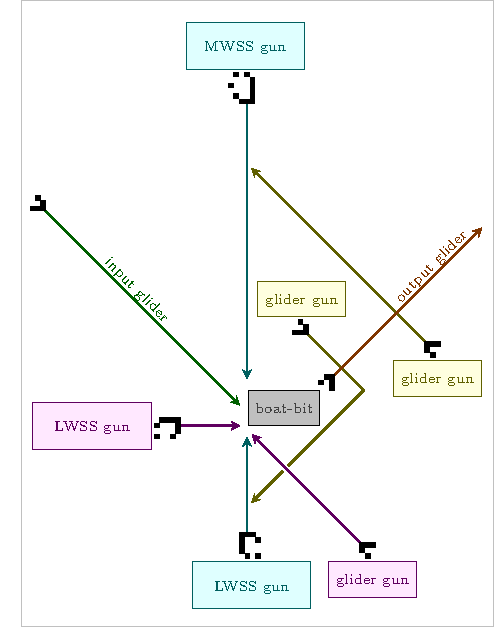
\includegraphics[width=1.02\textwidth]{periodic_circuitry/regulator_schematic.pdf}
		\caption{A schematic for the universal regulator.}
		\label{fig:universal_regulator_schematic}
	\end{subfigure} \ \ \ \ % 
	\begin{subfigure}{.48\textwidth}
		\centering
		\begin{tikzpicture}[scale=0.9]%
			\draw (-0.29,5.69) node[anchor=north west]{\patternimglink{0.076}{universal_regulator_periodic}};
			
			% BORDER
			\draw[gridgray] (-0.2,5.59) -- (7.8,5.59) -- (7.8,-5) -- (-0.2,-5) -- cycle;
		\end{tikzpicture}
		\caption{A period~$60$ implementation of the regulator.}
		\label{fig:universal_regulator_periodic_real}
	\end{subfigure}
	\caption{A universal regulator's (a) schematic and (b) period~$60$ implementation. This device takes in a glider with \emph{any} timing from the northwest input lane and produces an output glider along the northeast lane with timing that is synchronized to some period (both lanes are highlighted in \bgbox{aquaback}{aqua}). The left LWSS gun and bottom-right glider gun (highlighted in \bgbox{orangeback2}{orange}) are used to create the duoplet spark reaction from Figure~\ref{fig:make_sync_glider} that is at the heart of the regulator. The top MWSS gun and bottom LWSS gun (highlighted in \bgbox{greenpastel}{green}) then rebuild the central eater~1 (thus allowing more input gliders), but only if the output glider has destroyed a glider from each of the suppressing glider streams (highlighted in \bgbox{yellowback2}{yellow}). Note that the rightmost suppressing glider path in the final regulator (b) was adjusted for spacing reasons.}\label{fig:universal_regulator_periodic}
\end{figure}

% Note repeat time 355 somewhere


%%%%%%%%%%%%%%%%%%%%%%%%%%%%%%%%
\section*{Notes and Historical Remarks}
\label{sec:periodic_circuits_notes}
\addcontentsline{toc}{section}{\nameref{sec:periodic_circuits_notes}}
%%%%%%%%%%%%%%%%%%%%%%%%%%%%%%%%

Because of their simplicity, many of the period~$30$ and period~$46$ mechanisms that we investigated in this chapter were discovered as early as the 1970s and '80s, so most of the earliest ``interesting'' patterns that were constructed in Conway's Game of Life make use of these components. Dean Hickerson built many of the most well-known of these constructions throughout the 1990's, including the first primer (which made use of essentially the same techniques, but slightly different components, as the one we constructed in Section~\ref{sec:primer}). Some other interesting constructions that he made mostly from these components include:\smallskip

\begin{itemize}
	\item A \emph{twin primer}\index{twin primer}---a gun that emits a stream of lightweight spaceships with the property that the $n$-th spaceship in the stream is present if and only if both $n-2$ and $n$ are prime (see Exercise~\ref{exer:twin_primer}). This pattern is particularly interesting since it is currently unknown whether or not there are infinitely many twin primes (in fact, this is one of the biggest open problems in number theory), so it is unknown whether or not it emits infinitely many lightweight spaceships.\smallskip
	
	\item A pseudo-random glider generator based on using the toggle from Figure~\ref{fig:toggle} within a glider loop. If the output from a toggle is looped around and fed back into itself, the resulting stream of gliders ends up looking almost completely random as it turns itself off and on in increasingly erratic intervals. If we then place a glider duplicator somewhere on the loop, this random-looking stream of gliders can be emitted as an extremely high-period gun.
	
	Specifically, if there is space for $n$ gliders in the loop and we think of the $k$-th emitted glider as a bit $b(k)$ (where the $k$-th glider's presence means $b(k) = 1$ and its absence means $b(k) = 0$), then the effect of the toggle is that $b(k) = b(k-1) \oplus b(k-n)$ for all $k > n$.\footnote{Here, $\oplus$ refers to the XOR or mod~$2$ addition of two bits. That is, $0 \oplus 0 = 1 \oplus 1 = 0$ and $0 \oplus 1 = 1 \oplus 0 = 1$.} This sequence of bits is extremely erratic and can have very large period even when $n$ is relatively small \cite{A046932}. For example, the $n = 25$ case is illustrated in Figure~\ref{fig:prng_gun}, where the period of the sequence of bits is $10\,961\,685$ and thus the period of the gun itself is $30 \times 10\,961\,685 = 328\,850\,550$.
	
	Guns producing wildly different sequences of gliders and with wildly varying periods can be constructed by changing the length of the glider loop (see Exercise~\ref{exer:prng_gun}).\bigskip
	
	\noindent\begin{minipage}{\linewidth}
		\centering\addtocounter{subfigure}{-2}% needed since for some reason the subfigure captioning starts at (c) without the -2 modifier
		\begin{minipage}{.57\textwidth}
			\centering\patternimglink{0.095}{prng_gun}
			\captionof{subfigure}{the pseudo-random gun}
		\end{minipage} \ \ \ \ % 
		\begin{minipage}{.39\textwidth}\vspace*{0.1cm}
			\texttt{1111111111111111111111111}\\
			\texttt{0101010101010101010101010}\\
			\texttt{0110011001100110011001100}\\
			\texttt{0100010001000100010001000}\\
			\texttt{0111100001111000011110000}\\
			\texttt{0101000001010000010100000}\\
			\texttt{0110000001100000011000000}\\
			\texttt{0100000001000000010000000}\\
			\texttt{0111111110000000011111111}\\
			\texttt{1010101011111111101010101}\\
			\texttt{0011001101010101001100110}\\
			\texttt{0010001001100110001000100}\\
			\texttt{0011110001000100001111000}\\
			\texttt{0010100001111000001010000\ensuremath{{}\, \cdots}}
			\captionof{subfigure}{the first 400 bits of its output}
		\end{minipage}
		\captionof{figure}{A period $30 \times 10\,961\,685 = 328\,850\,550$ pseudo-random glider gun. It sends gliders around a $25 \times 30 = 750$-generation track (highlighted in \bgbox{aquaback}{aqua}) that contains a toggle (highlighted in \bgbox{greenpastel}{green}) and the glider duplication/inversion reaction introduced in Figure~\ref{fig:stream_inverter} (highlighted on the right in \bgbox{yellowback2}{yellow}). By feeding the output of the toggle back into itself, the arrangement of $25$ gliders along the track becomes quite unpredictable and random-looking, and thus so does the output glider stream (highlighted in \bgbox{magentaback}{magenta}) that follows the $10\,961\,685$-bit string whose first $400$ bits are displayed in~(b).}\label{fig:prng_gun}\bigskip
	\end{minipage}

	\item A pattern that uses four breeders that aim Gosper glider guns so as to repeatedly invert each other and have asymptotic growth related to $\pi \approx 3.14159$. This pattern fills the plane with triangular regions that alternate back and forth between being filled and being empty.

	Specifically, if we use $T(n,t)$ to denote the triangle in the northeast quadrant with vertices at $(0,0)$ (i.e., the center of the pattern), $(0, t/(2n))$, and $(t/(2(n+2)), 0)$, then in generation~$t$ the triangle $T(1,t)$ is filled with gliders except that the smaller triangle $T(3,t)$ within it is empty, except that the smaller triangle $T(5,t)$ within it is filled with gliders, except that $T(7,t)$ is empty, and so on (see Figure~\ref{fig:life_computes_pi}).\bigskip
	
	\noindent\begin{minipage}{\linewidth}
		\centering\embedlink{life_computes_pi}{\vcenteredhbox{\patternimg{0.101}{life_computes_pi_0}} \vcenteredhbox{$\xrightarrow{\text{\clock{12}{45} 4500}}$} \vcenteredhbox{\patternimg{0.125}{life_computes_pi_5000}}} % genarrow does not work with input as large as 5000
		\captionof{figure}{An arrangement of four breeders (highlighted in \bgbox{yellowback2}{yellow}) that produce Gosper glider guns that fire at each other so as to invert each others' streams (shown on the left after the breeders have been moving away from each other for $500$~generations). In generation $t$ (shown here on the right with $t = 5000$), the \bgbox{greenpastel}{green} triangular region $T(1,t)$ is filled with gliders, except the \bgbox{aquaback}{aqua} triangular region $T(3,t)$ is empty, except the \bgbox{magentaback}{magenta} triangular region $T(5,t)$ is filled with gliders, and so on.}\label{fig:life_computes_pi}\bigskip
	\end{minipage}
	
	Since the triangle $T(n,t)$ has area
	\[
		\frac{1}{2} \times \frac{t}{2n} \times \frac{t}{2n+4} = \frac{t^2}{16} \left(\frac{1}{n} - \frac{1}{n+2}\right),
	\]
	the occupied area in the first quadrant in generation~$t$ (when $t$ is large) is approximately
	\begin{align*}
		T(1,t) - T(3,t) + T(5,t) - \cdots & = \frac{t^2}{16} \left( \left(1 - \frac{1}{3}\right) - \left(\frac{1}{3} - \frac{1}{5}\right) + \left(\frac{1}{5} - \frac{1}{7}\right) - \cdots\right) \\
		& = \frac{t^2}{16} \left( 1 - \frac{2}{3} + \frac{2}{5} - \frac{2}{7} + \cdots\right) \\
		& = \frac{t^2}{16}\big( 2\arctan(1) - 1\big) = \frac{(\pi-2)t^2}{32},
	\end{align*}
	where the second-to-last equality follows from the fact that $\arctan(x)$ has Taylor series $\arctan(x) = x - x^3/3 + x^5/5 - \cdots$, so $\arctan(1) = 1 - 1/3 + 1/5 - \cdots$, and the final equality holds because $\arctan(1) = \pi/4$.
	
	Since the gliders fill this occupied area with density $1/90$ and this same calculation applies to all four quadrants of the plane, we see that this pattern's population in generation~$t$ (again, when $t$ is large) is approximately
	\[
		\frac{4}{90} \times \frac{(\pi-2)t^2}{32} = \frac{(\pi-2)t^2}{720}.
	\]
\end{itemize}

In fact, John Conway and Bill Gosper used little more than some basic period~$30$ circuitry way back in 1982 \cite[Chapter~25]{BCG82} to demonstrate that the Game of Life is \emph{universal}---anything that can be computed (by a regular computer, for example), can be computed in the Game of Life by cleverly arranging some period~$30$ circuitry and manipulating gliders. Thus, for example, we knew that prime numbers could be computed in the Game of Life almost a decade before the first primer was explicitly constructed.

The advantage of the new circuitry and constructions that we have available to us now is that they are significantly smaller than the ones that would result from implementing the construction outlined by Conway and Gosper's universality proof \index{computational universality} (which require sending gliders across absolutely vast distances for even the simplest of computations). There is also something quite appealing about having \emph{explicit} constructions of these patterns---actually arranging the components in Conway and Gosper's constructions so as to have the correct positioning and timing would typically be infeasible in practice, and the resulting patterns would not be terribly interesting to look at.



%%%%%%%%%%%%%%%%%%%%%%%%%%%%%%%%%
\section*{Exercises \hfill \normalfont\textsf{\small solutions on \hyperlink{solutions_periodic_circuitry}{page \pageref{solutions_periodic_circuitry}}}}
\label{sec:periodic_exercises}
\addcontentsline{toc}{section}{Exercises}
\vspace*{-0.4cm}\hrulefill\vspace*{-0.3cm}\footnotesize\begin{multicols}{2}\vspace*{-0.4cm}\raggedcolumns\interlinepenalty=10000
\setlength{\parskip}{0pt}
%%%%%%%%%%%%%%%%%%%%%%%%%%%%%%%%%


\begin{problem}\label{exer:inline_inverter_gun_why_buckaroo}
	In the glider gun in Figure~\ref{fig:inline_inverter_p120_gun}, we used eater~1s instead of blocks to stabilize some of the Gosper glider guns (as in the buckaroo of Figure~\ref{fig:buckaroo}). Explain why.
\end{problem}


\mfilbreak


\begin{problem}\label{exer:inline_inverter_gun_high_period}
	Construct a glider gun based on the inline inverter with...\smallskip
	
	\begin{enumerate}[label=\bf\color{ocre}(\alph*)]
		\item period~$240$.
			
		\item period~$360$.
	\end{enumerate}
\end{problem}


\mfilbreak


\begin{problem}\label{exer:inline_inverter_advancer}
	Use two inline inverters to create a pattern that advances a stream of gliders by $20$ generations, similar to how the fast forward force field\index{fast forward force field} of Figure~\ref{fig:fast_forward_force_field} advances a stream of lightweight spaceships.
\end{problem}
% Signal-circuitry/advancer.rle uses 6 inline inverters to advance gliders quicker than c/4
	
	
\mfilbreak
	
	
\begin{problem}\label{exer:inline_inverter_lwss_gun}
	Construct a period~$240$ lightweight spaceship gun...\smallskip
	
	\begin{enumerate}[label=\bf\color{ocre}(\alph*)]
		\item using three inline inverter guns.
		
		\item using one inline inverter gun and the reaction from Figure~\ref{fig:glider_to_lwss}.
	\end{enumerate}
\end{problem}


\mfilbreak


\begin{problem}\label{exer:make_inline_inverter_with_weird_period}
	Use the reaction from Figure~\ref{fig:stream_inverter}, together with reflectors and eaters as necessary, to create an inline inverter with for a glider stream with...\smallskip
	
	\begin{enumerate}[label=\bf\color{ocre}(\alph*)]
		\item period~$43$.
		
		\item period~$36$.
		
		\item period~$25$.
	\end{enumerate}
\end{problem}


\mfilbreak


% p240 gun was given in this chapter, so this exercise is OK
\begin{problem}\label{exer:twin_prime_gun}\index{twin prime}
	A pair of positive integers $(p,p+2)$ is called a \emph{twin prime pair} if they are both prime. Find a way of aiming a p$240$ glider gun at the output LWSS stream of the primer from Figure~\ref{fig:primer} so that the resulting LWSS stream now corresponds to twin prime pairs, rather than all prime numbers.
	
	\noindent [Hint: Position the glider gun so that the glider destroys an LWSS, creating a small still life that then blocks the next glider (and lets the next LWSS, if present, pass). Do not worry about the first two twin prime pairs ($(3,5)$ and $(5,7)$ are the only twin prime pairs that overlap), and do not worry about whether the gun outputs the lower or upper number in each twin prime pair.]
\end{problem}


\mfilbreak


\begin{problem}\label{exer:glider_to_hwss_to_glider}
	The periodic circuits displayed below can be used to convert two gliders into an HWSS and an HWSS back into a glider.\footnote{These reactions were found and simplified by a combination of David Buckingham, Bill Gosper, Dieter Leithner, and Peter Rott.}
	\begin{center}
		\patternimglink{0.1}{glider_to_hwss_to_glider}
	\end{center}
	\begin{enumerate}[label=\bf\color{ocre}(\alph*)]
		\item Use the left reaction to create a period~$120$ HWSS gun.
		
		\item Create a glider loop that uses both of these reactions to convert the glider into an HWSS and back.
	\end{enumerate}
\end{problem}
% (b) solution:
%x = 80, y = 42
%47b2o$47bo$35bo9bobo$33bobo9b2o$32bobo$26b2o3bo2bo$26b2o4bobo$33bobo$
%35bo3$32b2o$32bo$23bo6bobo$23bobo4b2o3bo$6b2o18b2o6bo$4bo3bo17b2o6b3o$
%3bo5bo16b2o$2b2obo3bo8bo4bobo$3bo5bo9bo3bo$4bo3bo5bo2b3o$6b2o2$3bo$2bo
%bo$bo3bo$2b3o21bo$2o3b2o17bobo45bo4bo$25b2o43b2ob4ob2o$72bo4bo2$15b2ob
%2obo$14b2o2b2ob2o$22bo41bo2bo$14b2o51bo$14b2o5b2o4b2o34bo4bo$21b2o3bob
%o5b2o27b2o2bobo$14bo12bo6bo33bob2o$3b2o9b2ob2o2b2o12b3o$3b2o10bob2ob2o
%15bo$68bo2bo$68b2o!


\mfilbreak


\begin{problem}\label{exer:any_wss_to_glider}
	The arrangement of queen bees below can be used to convert any of the lightweight, middleweight, or heavyweight spaceships into gliders.
	\begin{center}
		\patternimglink{0.1}{any_wss_to_glider}
	\end{center}
	\begin{enumerate}[label=\bf\color{ocre}(\alph*)]
		\item Use this reaction as well as one of the reactions from Exercise~\ref{exer:glider_to_hwss_to_glider} to create a glider loop that converts a glider into an HWSS and back.
		
		\item Use this reaction to create a gun that emits a glider stream (rather than an LWSS stream as in Figure~\ref{fig:primer}) that is spaced according to the prime numbers.
	\end{enumerate}
\end{problem}


\mfilbreak


\begin{problem}\label{exer:glider_to_lwss_loop}
	Construct an oscillator that makes use of the reactions in each of Figures~\ref{fig:glider_to_lwss} and~\ref{fig:lwss_to_glider} to send a glider around a track in such a way that it is converted into an LWSS and back during each loop.
\end{problem}
%x = 73, y = 52, rule = B3/S23
%29b2o19b2o$30bo19bo$30bobo8bo6bobo$31b2o5b4o6b2o$37b4o$37bo2bo$37b4o$
%38b4o$41bo2$38bo$36bobo$37b2o5$21bo$21b2o$20bobo3$4b2o$2bo4bo$bo6bo$o
%8bo43bo$o8bo41bobo$o8bo15b4o23b2o6b2o$bo6bo16bo3bo30bobo$2bo4bo17bo29b
%2o6bo$4b2o20bo2bo24bo2bo2bo2bo7b2o$16bo38b2o6bo7b2o$16bo43bobo$15b3o
%42b2o2$55b3o$15b3o37b3o$16bo37bo3bo$16bo36bo5bo$16bo37bo3bo$16bo38b3o$
%15b3o3$15b3o$16bo$16bo4$56b2o$56b2o!


\mfilbreak


\begin{problem}\label{exer:period_not_235_gun}
	Construct a pattern that emits a stream of lightweight spaceships with the property that the $n$-th spaceship in the stream is present if and only if $n$ is not a multiple of $2$, $3$, or $5$.
\end{problem}


\mfilbreak


\begin{problem}\label{exer:rewind_primer}
	One method of making a pattern smaller is to change it into the form that it would have looked several generations earlier (this is called \emph{rewinding}\index{rewind} the pattern). Use this technique, along with moving its various components closer together, to reduce the size of the bounding box of the primer from Figure~\ref{fig:primer} from $951 \times 696 = 661,896$ to $500,000$ or less.
\end{problem}


\mfilbreak


\begin{problem}\label{exer:twin_primer}
	The collision of a glider with an LWSS shown below is called a \emph{filter}\index{filter}. It results in a single block that destroys the next incoming glider, letting the next incoming LWSS pass by unharmed, thus doubling the period of the LWSS stream.
	
	Add this reaction (and potentially some guns and eaters, as necessary) to the primer to create a \emph{twin primer}\index{twin primer}---a pattern that creates a stream of lightweight spaceships for which the $n$-th LWSS in the stream is present if and only if $n-2$ and $n$ are both prime.

	\begin{center}
		\embedlink{exercise_lwss_filter}{\vcenteredhbox{\patternimg{0.1}{exercise_lwss_filter_0}} \vcenteredhbox{\genarrow{6}} \vcenteredhbox{\patternimg{0.1}{exercise_lwss_filter_6}}}
	\end{center}
\end{problem}


\mfilbreak


\begin{problem}\label{exer:twin_bees_loop}
	Use the patterns from Figure~\ref{fig:twin_bees_reflect} to create a loop oscillator in which a glider is converted into a lightweight spaceship and back at some point in the loop.
\end{problem}


\mfilbreak


\begin{problem}\label{exer:twin_bees_mwss_gun}
	Use the patterns from Figure~\ref{fig:twin_bees_weird_guns} to construct a period~$46$ middleweight spaceship gun.
\end{problem}


\mfilbreak


\begin{problem}\label{exer:ticker_tape_gun_store_different}
	Modify the sequence of gliders in the loop of the gun from Figure~\ref{fig:ticker_tape_gun} so that it produces lightweight spaceships corresponding to the bitstring ``110111010011011101001''.
\end{problem}


\mfilbreak


\begin{problem}\label{exer:ticker_tape_smiley_gun}
	Using the techniques used in Figure~\ref{fig:ticker_tape_hi_gun}, create a ticker tape gun that produces smiley faces.
\end{problem}


\mfilbreak


\begin{problem}\label{exer:ticker_tape_gun_memory_alter}
	Fire some gliders at the memory cell\index{memory cell} from Figure~\ref{fig:p46_memory_cell} so as to change the bitstring that it stores to ``101010101010''.
\end{problem}


\mfilbreak


\begin{problem}\label{exer:tanners_p46_twin_bee_gun}
	Create a glider gun that makes use of a single copy of Tanner's p$46$ and twin bees that are stabilized only on one side. [Hint: You want the spark from these two objects to hit each other. This gun can be found by hand via trial error, or you could write a computer program to try lots of positionings.]
\end{problem}
% NOTE: Found by David Bell
% SOLUTION:
%x = 31, y = 44
%17boo5boo$17boo5boo11$17bo7bo$15boboo5boobo$15bo3booboo3bo$16bo3bobo3b
%o$17b3o3b3o10$14bo14bo$13b3o14bo$12bobobo11b3o$12bobobo$10boob3oboo$9b
%obooboboobo$3boo3boobo5boboo$3boo4boobo3boboobboboo$10b3o3b3o3boobo$$
%bboo$3bo$3o$o13bo$13boboboboo$12bobooboobo$12bo$11boo!


\mfilbreak


\begin{problem}\label{exer:tanners_p46_reflect}
	Show how Tanner's p$46$ can be used to reflect a glider by 180~degrees. [Hint: The spark emitted by Tanner's p$46$ is quite similar to some of the sparks emitted by the pentadecathlon. Mimic the reflection from Figure~\ref{fig:p30_relay}.]
\end{problem}
% NOTE: Found by David Bell
% SOLUTION:
%x = 209, y = 182
%201b8o$201bob4obo$201b8o155$4boo$5bo28boo$5bobo25bobo$6boobboo23bo$10b
%oo7$o$3o7boo$3bo6boo$bbobo7bo$bboo6boo$10boo$bboo$bbo$3b3o$5bo$8boo$9b
%o$6b3o$6bo!


\mfilbreak


\begin{problem}\label{exer:twin_bees_large_spark}
	An arrangement of two twin bees shuttles that is particularly useful due to the extremely large spark that it produces is displayed below.
	
	\begin{center}
		\patternimglink{0.1}{twin_bees_large_spark}
	\end{center}
	
	\begin{enumerate}[label=\bf\color{ocre}(\alph*)]
		\item Collide the spark from this object with that of Tanner's p$46$ to create a glider gun. [Hint: Writing a computer program might be helpful here.]
		
		\item Collide the spark from this object with the following arrangement of twin bees and an eater~1 to create a double-barreled glider gun\index{double-barreled gun} (i.e., a gun that emits two side-by-side gliders per period).\footnote{This double-barreled gun was originally found by Dieter Leithner.}
		
		\begin{center}
			\patternimglink{0.1}{twin_bees_partial_double_barrel}
		\end{center}
	\end{enumerate}
\end{problem}
% Shows up in vaccuum gun and also p46 gliderless HWSS gun (twice)
% Solution for (a), but there are at least 6 others too:
%28b2o$28bo$26bobo$17b2o7b2o$2o14b2ob2o$2o15bo2bo$17bo2bo$18b2o2$18b2o$
%17bo2bo$2o15bo2bo$2o14b2ob2o12b2o14b2o$17b2o13b2o15b2o$33b5o$34b4o2$
%34b4o$33b5o$32b2o15b2o$33b2o14b2o14$21bo$20b3o$19b5o$18b2o3b2o$17b2o5b
%2o5b2o$18b2o3b2o6b2o$13b2o4bo3bo$12bobo$12bo19b2o$11b2o19bo$33b3o$21bo
%13bo$15b2obobobo$15bob2ob2obo$23bo$23b2o!
% Solution for (b):
%b2o23b2o$b2o23bo$24bobo$8b2o14b2o$2o5bobo$2o5bo$7b3o$23b2o$25bo18b2o$
%21bo2b2o18b2o$7b3o10b3obo9bo$2o5bo12bo3bo7bo2bo$2o5bobo9b5o8b5o8b2o$8b
%2o10bob3obo5b3ob2o7b2o$20b2obo3bo5b2obo$b2o21bobo7b2o$b2o21b2o$22b2o
%10b2o$21bo2bo8b2obo$24bo7b3ob2o7b2o$21bo2bo7b5o8b2o$22b3o7bo2bo$34bo$
%44b2o$44b2o5$31bo$30b2o15b2o$29b2o16b2o$30b2o2b2o4$30b2o2b2o$29b2o16b
%2o$30b2o15b2o$16b2o13bo$15bobo$15bo$14b2o!


\mfilbreak


\begin{problem}\label{exer:2eng_corder_gun}
	Use the $9$-glider synthesis from Exercise~\ref{exer:2_engine_cordership_synthesis} to construct a gun that fires $2$-engine Corderships.
\end{problem}
% Numerous possible solutions here: https://www.conwaylife.com/forums/viewtopic.php?t=&p=54750#p54750


\mfilbreak


\begin{problem}\label{exer:bumper_bouncer_wrong_color}
	Explain why it is not possible to construct glider loop oscillators consisting only of the following sets of reflectors, and experiment with them to convince yourself that they really are impossible.\smallskip
	
	\begin{enumerate}[label=\bf\color{ocre}(\alph*)]
		\item Three bumpers and one bouncer.
		
		\item Three bouncers and one Snark.
	\end{enumerate}
\end{problem}


\mfilbreak


\begin{problem}\label{exer:bumper_high_period}
	Construct a bumper reflector with...\smallskip
	
	\begin{enumerate}[label=\bf\color{ocre}(\alph*)]
		\item period~$16$.
		
		\item period~$22$.
		
		\item period~$15$. [Hint: Try using the sparker from Figure~\ref{fig:p15_bouncer}.]
		
		\item period~$5$. [Hint: Try modifying the sparker from Figure~\ref{fig:p5_bouncer}.]
		
		\item period~$4$, making use of the fountain\index{fountain} sparker. % UPDATE
	\end{enumerate}
\end{problem}


\mfilbreak


\begin{problem}\label{exer:p11_bumper_not_useful}
	Explain why the period~$11$ bumper from Figure~\ref{fig:p11_bumper} is not useful for glider streams of period below $121$. [Hint: You can use smaller bumpers in place of it.]
\end{problem}


\mfilbreak


\begin{problem}\label{exer:minimum_period_snark_loop}
	The smallest-period single-glider Snark loop has period~$216$ and is displayed in Figure~\ref{fig:minimum_snark_loop}. Note that the still life in the center of this loop is the weld of four eater~1s from Exercise~\ref{exer:eater_weld}(c).\smallskip
	
	\begin{enumerate}[label=\bf\color{ocre}(\alph*)]
		\item Move each of the Snarks outward by $1$~cell (e.g., move the northern Snark north by $1$ cell) and un-weld the central eater~$1$s. What is the period of the resulting glider loop? Explain how you could have determined this period without explicitly constructing this modified glider loop.
		
		\item Replace the Snarks in the glider loop from part~(a) by p$4$~bumpers in a way that keeps the glider on the same lanes. What is the period of the resulting glider loop? Explain how you could have determined this period without explicitly constructing this modified glider loop.
		
		\item Replace one of the p$4$ bumpers in the glider loop from part~(b) with a p$6$ bumper.
		
		\item If you replace one of the p$4$ bumpers in the glider loop from part~(b) with a p$5$ bumper, the loop stops working. Why?
		
		\item Move the bumpers in the glider loop from part~(b) closer together so as to alter the period of the loop. Once you have made a loop with a suitable period, replace one of the p$4$ bumpers by a p$5$ bumper.
	
		\noindent\begin{minipage}{\linewidth}
			\centering
			\patternimglink{0.1}{minimum_snark_loop}
			\captionof{figure}{\footnotesize A single-glider loop built from Snarks with the smallest possible period---$216$.}\label{fig:minimum_snark_loop}\medskip
		\end{minipage}
	\end{enumerate}
\end{problem}


\mfilbreak


\begin{problem}\label{exer:p29_pipsquirter}
	Use the \emph{skewed p$29$ pre-pulsar shuttle}\index{pre-pulsar shuttle} displayed below to create a p$29$ bouncer reflector.\footnote{This reflector was originally found by Matthias Merzenich in August 2013.}
	
	\begin{center}
		\patternimglink{0.1}{skewed_p29}
	\end{center}
\end{problem}


\mfilbreak


\begin{problem}\label{exer:p60_regulator_mwss_emulator}
	The lightweight spaceship guns in Figure~\ref{fig:universal_regulator_periodic_real} each contain a middleweight emulator. Describe what role this oscillator plays in the gun.
\end{problem}


\mfilbreak


\begin{problem}\label{exer:p60_regulator_reflectors}
	Two reflectors are highlighted in magenta in Figure~\ref{fig:universal_regulator_periodic_real}. Identify these reflectors (we have discussed them each earlier).
\end{problem}


\mfilbreak


\begin{problem}\label{exer:prng_gun}
	Changing the number of gliders in the loop portion of the pseuro-random glider-generating gun from Figure~\ref{fig:prng_gun} can drastically change its period.\smallskip
	
	\begin{enumerate}[label=\bf\color{ocre}(\alph*)]
		\item If you move the northwest portion of the loop northwest by an additional $15$~cells (and rephase reflectors as necessary), how many additional gliders fit in the loop?
		
		\item Determine the period of the gun constructed in part~(a). [Hint: Computer software may be useful here---it is massive.]
		
		\item Move the northwest portion of the loop northwest by an \emph{additional} $15$~cells (again, rephase reflectors as necessary). Determine the period of this gun. [Hint: Its period is now small enough that you \emph{may} be able to compute it by hand if you are clever.]
	\end{enumerate}
\end{problem}

% Exercise with J Summers' gunless primer?

% USe Tanner's p46 to make a p690 oscillator
% Solution: http://conwaylife.com/forums/viewtopic.php?f=2&t=1437&start=425#p52234

% EXERCISE: Use this glider-producing collision to make a p23 glider gun via stream merging:
%x = 68, y = 34, rule = B3/S23
%39bo$b2o27b3o$b2o18b2o5bo4bo11b2o$28bo5bo10b2o$13b2o18bo$2o9b2o2bo15b
%2o$2o9b6o$11b4o16b2o$24bo8bo$25bo2bo5bo$23b3o2bo4bo31b2o$11b4o15b3o32b
%2o$2o9b6o$2o9b2o2bo$13b2o26b2o8b3o12b2o$41b2o8bo3bo10b2o$b2o48bo4bo$b
%2o49bo3bo2$52bo3bo$36bo14bo4bo$34bobo14bo3bo10b2o$24bo10b2o14b3o12b2o$
%7b2o15b2o$7b2o16b2o$20b2o2b2o39b2o$40bobo22b2o$41b2o$41bo$20b2o2b2o$7b
%2o16b2o7b2o$7b2o15b2o8b2o11bo$24bo23bo$46b3o!


% EXERCISE: create a p23 glider gun using this reflection
%x = 38, y = 49, rule = B3/S23
%22bo$23bo$21b3o3$29bo$29bobo$29b2o$25b2o$10b2o13b2o$2o6b2ob2o11b3o$2o
%6bo2bo9bob4o$8bo2bo8bo4bo$9b2o14bo$24bo$9b2o$8bo2bo10b2o$8bo2bo$8b2ob
%2o$10b2o$34b2o$34b2o8$28bo5bo$27b3o3b3o$26b2obo3bob2o3$29bo3bo$29bo3bo
%5$34bo$33bobo$32b2ob2o$32bo3bo$31b3ob3o$32bo3bo$32bo3bo$27b2o4bobo$27b
%2o5bo!

% EXERCISE: Construct a p46 glider duplicator

% p46 ege shooter based on twin bees?
%x = 67, y = 82, rule = B3/S23
%3$47b2o5b2o$47b2o5b2o7$48bo5bo$47b3o3b3o$46bo2b2ob2o2bo$46b3o5b3o9$47b
%3o$46bo3bo$46b2ob2o$47bobo2$47bobo$46b2ob2o$46bo3bo3b2o$47b3o4b2o2$39b
%obo2b2o$24b2o12bo3bob3o$24b2o13bo6b2o$40b5obo$43b3o2$43b3o$40b5obo$24b
%2o13bo6b2o$24b2o12bo3bob3o$39bobo2b2o7$38bobo$38b2o$39bo9$28bo$26b2o$
%27b2o10$15bobo$15b2o$16bo!

%% EXERCISE END COMMANDS
\end{multicols}
\normalsize\vspace*{0.01cm}
%% DONE EXERCISE END COMMANDS

%%%%%%%%%%%%%%%%%%%%%%%%%%%%%%%%%%%%%%%%%%%%%%%%%%%%%%%%%%%%%%%%%%%%%%%%%
%%   CHAPTER: STATIONARY CIRCUITRY
%%%%%%%%%%%%%%%%%%%%%%%%%%%%%%%%%%%%%%%%%%%%%%%%%%%%%%%%%%%%%%%%%%%%%%%%%

% TODO: Add (maybe as an exercise?) the Bandersnatch: https://www.conwaylife.com/wiki/Bandersnatch

\renewcommand{\chapterfolder}{stationary_circuitry/}
\chapterimage{cover/stationary_circuitry}

\chapter{Stable Circuitry}\label{chp:stationary_circuitry}


\vspace*{-0.4in}
\epigraph{The greatest use of a life is to spend it on something that will outlast it.}{William James}
\vspace*{0.4in}


\noindent In the previous chapter, we illustrated how we could manipulate gliders (and sometimes other moving objects like lightweight spaceships) via periodic components like oscillators. We now investigate how to similarly perform these tasks via stable objects (i.e., still lifes), which has the advantage of not restricting the period of the glider streams that can make use of the circuitry. We actually already know of some very important stable circuits, such as the Snark (a stable glider reflector) from Figure~\ref{fig:snark}, but typically they are more difficult to construct due to the fact that stable objects can not provide any sparks for gliders to make use of.

For this reason, stable circuitry typically focuses not just on manipulating gliders, but also on manipulating other (easier to manipulate) objects like Herschels, just as we did in Section~\ref{sec:herschel_track}. We will even spend quite a bit of time converting moving objects of one type into another type (e.g., a glider into a Herschel or vice-versa). We start by giving Herschel tracks a more thorough treatment.


\section{Herschel Conduits}\label{sec:conduits}\index{conduit}

There are numerous Herschel conduits other than the R64 and Fx77 conduits that we saw back in Figure~\ref{fig:herschel_conduits}. Although those two conduits suffice to create oscillators and guns of any sufficiently large period, certain periods are quite unwieldy. For example, the smallest period~$67$ oscillator or gun that can be created using just these two conduits requires $4$~R64 conduits and $28$~Fx77 conduits to make a track of length
\[
{\color{gray}\underbrace{\color{black}4 \times 64}_\text{R64 time}} \ + \ {\color{gray}\underbrace{\color{black}28\times 77}_\text{Fx77 time}} = 2{\thousep}412 = 36 \times 67 \text{ generations,}
\]
which we place $36$ equally-spaced Herschels on. However, if we extend our collection of conduits a little bit, then we can construct a Herschel-based period~$67$ gun that uses just $8$ Herschels on an $8 \times 67 = 536$-generation track made up of $4$ conduits, as in Figure~\ref{fig:p67_with_conduits}.\footnote{We saw one of these extra conduits, L112, way back in Exercise~\ref{exer:herschel_track_L112}.}

\begin{figure}[!htb]
	\centering
	\begin{tabular}{@{}cc@{}}
		\begin{subfigure}{.37\textwidth}
			\centering
			\patternimglink{0.105}{l112}
			\caption{the \emph{L112}\index{L112} conduit}
			\label{fig:l112_conduit}
		\end{subfigure} &
		\multirow{2}{*}{\renewcommand{\thesubfigure}{(c)}\begin{subfigure}{.59\textwidth}
				\centering\vspace*{-2cm}
				\patternimglink{0.2045}{p67_gun}
				\caption{a p$67$ glider gun}
				\label{fig:p67_gun}
		\end{subfigure}} \\[1.3cm]
		\renewcommand{\thesubfigure}{(b)}\begin{subfigure}{.37\textwidth}
			\centering\vspace*{0.2cm}
			\patternimglink{0.08976190476}{l156}
			\caption{the \emph{L156}\index{L156} conduit}
			\label{fig:l156_conduit}
		\end{subfigure}
	\end{tabular}
	\caption{A period~$67$ glider gun can be constructed from just four Herschel conduits. The track (c) uses two copies of the L112 conduit from~(a) (highlighted in \bgbox{yellowback2}{yellow}) and two copies of the L156 conduit from~(b) (highlighted in \bgbox{aquaback}{aqua}). Both of these conduits rotate an input Herschel (displayed in \bgbox{greenback}{green}) counter-clockwise by 90~degrees into the output position (displayed in \bgbox{orangeback}{orange}), with L112 taking 112~generations to do so and L156 taking 156~generations. Eaters displayed in \bgbox{redback}{red} are used to delete escaping gliders, but are not required for the conduits to function.}
	\label{fig:p67_with_conduits}
\end{figure}

The added flexibility of these additional conduits not only lets us greatly reduce the size of Herschel tracks, but also makes it much easier to position them in certain situations (if we want a Herschel to output a glider at a specific location or with a certain timing, for example). For this reason, it is useful to have a large list of Herschel conduits available to choose from. For ease of reference, conduits are named according to the orientation of the output Herschel relative to that of the input Herschel,\footnote{Be somewhat careful here---the naming does not care about the \emph{position} of the output Herschel relative to the input Herschel, only the change in its orientation.} together with the number of generations that it takes for the output Herschel to appear. For example, the R64 conduit is named that way because it turns the input Herschel to the \textbf{r}ight in \textbf{64} generations. More generally, the prefix used when naming conduits is one of:
\begin{align*}
	\text{\bf R:} & \ \text{right (clockwise) turn} & \text{\bf F:} & \ \text{forward (no turn)} \\
	\text{\bf L:} & \ \text{left (counter-clockwise) turn} & \text{\bf B:} & \ \text{backward (180-degree turn)}
\end{align*}

For example, the L112 and L156 conduits are named for the fact that they rotate a Herschel left (i.e., counter-clockwise) over the course of 112 and 156 generations, respectively. We also insert an ``x'' between two parts of the conduit's name if it mirrors the Herschel (as in the Fx77 conduit from Figure~\ref{fig:Fx77}).\footnote{To make the ``x means mirror'' notation unambiguous, we need to specify the direction in which the mirroring is done, so we (arbitrarily) choose to mirror along the single side of the Herschel that is perpendicular to its other two sides (if you prefer, you can simply refer to Figure~\ref{fig:herschel_orientations} to see how the mirroring is done).} A conduit's name can thus have one of $8$ possible prefixes (i.e., R, Rx, L, Lx, F, Fx, B, or Bx) corresponding to the $8$ possible orientations of the output Herschel that they produce, as indicated in Figure~\ref{fig:herschel_orientations}.

\begin{figure}[!htb]
	\centering\begin{tikzpicture}[scale=0.8, every node/.style={transform shape}]%
	\node[inner sep=0pt,anchor=south west] at (0,0) {\patternimglink{0.12}{herschel_orientations}};
	
	\colorletternode{gray}{1.9}{1.42}{F}
	\colorletternode{gray}{3.49}{1.42}{Fx}
	\colorletternode{gray}{4.81}{1.34}{R}
	\colorletternode{gray}{6.59}{1.34}{Rx}
	\colorletternode{gray}{8.05}{1.42}{B}
	\colorletternode{gray}{9.63}{1.42}{Bx}
	\colorletternode{gray}{10.84}{1.34}{L}
	\colorletternode{gray}{12.66}{1.34}{Lx}
	\end{tikzpicture}
	\caption{Herschels can be oriented in one of $8$ ways, which we label here relative to the (arbitrarily-chosen) canonical input orientation displayed on the left in \bgbox{greenback}{green}.}\label{fig:herschel_orientations}
\end{figure}

With this naming scheme out of the way, we now catalog some of the smallest, quickest, and most useful Herschel conduits that are known in Table~\ref{tab:herschel_conduits}. Keep in mind that this list is nowhere near complete---there are well over 100 known Herschel conduits made up of small still lifes.\footnote{For a reasonably complete collection of known small Herschel conduits, see \httpsurl{conwaylife.com/forums/viewtopic.php?f=2\&t=2347}} All of these conduits release at least one glider and can thus be used to construct guns, but of particular note is L156, which releases a glider from its corner in a somewhat different orientation than most of the others (we made use of this glider in the period~$67$ gun from Figure~\ref{fig:p67_with_conduits}). It is also worth finding the R64, Fx77, L112, and L156 conduits that we are already familiar with in this table, to see where they fit in with other Herschel conduits.

\begin{table}[!htp]
	\begin{center}
		\begin{tabular}{Sc Sc Sc Sc Sc Sc}
			\toprule
			& \multicolumn{2}{c}{Rotating conduits} & & \multicolumn{2}{c}{Rotating and reflecting conduits} \\\midrule
			\begin{minipage}[b]{0.02\textwidth}\centering F: \\ ${}$ \\ ${}$ \\ ${}$\end{minipage} & \begin{minipage}[b]{0.19\textwidth}\centering\patternimglink{0.10957705395}{f116} \\ F116\index{F116} (138)\end{minipage} & \begin{minipage}[b]{0.22\textwidth}\centering\patternimglink{0.10417437697}{f117} \\ F117\index{F117} (63)\end{minipage} & \specialcell{ } & \begin{minipage}[b]{0.2\textwidth}\centering\patternimglink{0.1262745098}{fx77} \\ Fx77\index{Fx77} (57)\end{minipage} & \begin{minipage}[b]{0.19\textwidth}\centering\patternimglink{0.1}{fx119} \\ Fx119\index{Fx119} (231)\end{minipage} \\
			
			\rowcolor{gray!20} \begin{minipage}[b]{0.02\textwidth}\centering R: \\ ${}$ \\ ${}$ \\ ${}$\end{minipage} & \begin{minipage}[b]{0.19\textwidth}\centering\patternimglink{0.137}{r64} \\ R64\index{R64} (61)\end{minipage} & \begin{minipage}[b]{0.22\textwidth}\centering\patternimglink{0.14202752293}{r126} \\ R126\index{R126} (125)\end{minipage} & \specialcell{ } & \begin{minipage}[b]{0.2\textwidth}\centering\patternimglink{0.09133676091}{rx140} \\ Rx140\index{Rx140} (260)\end{minipage} & \begin{minipage}[b]{0.19\textwidth}\centering\patternimglink{0.085}{rx164} \\ Rx164\index{Rx164} (65)\end{minipage} \\
			
			\begin{minipage}[b]{0.02\textwidth}\centering B: \\ ${}$ \\ ${}$ \\ ${}$\end{minipage} & \begin{minipage}[b]{0.19\textwidth}\centering\patternimglink{0.14}{b60} \\ B60\index{B60} (43)\end{minipage} & \begin{minipage}[b]{0.22\textwidth}\centering\patternimglink{0.08820895522}{b245} \\ B245\index{B245} (278)\end{minipage} & \specialcell{ } & \begin{minipage}[b]{0.2\textwidth}\centering\patternimglink{0.1049112426}{bx106} \\ Bx106\index{Bx106} (134)\end{minipage} & \begin{minipage}[b]{0.19\textwidth}\centering\patternimglink{0.09}{bx202} \\ Bx202\index{Bx202} (65)\end{minipage} \\
			
			\rowcolor{gray!20} \begin{minipage}[b]{0.02\textwidth}\centering L: \\ ${}$ \\ ${}$ \\ ${}$\end{minipage} & \begin{minipage}[b]{0.19\textwidth}\centering\patternimglink{0.10904761904}{l112_table} \\ L112\index{L112} (58)\end{minipage} & \begin{minipage}[b]{0.22\textwidth}\centering\patternimglink{0.09325791855}{l156_table} \\ L156\index{L156} (62)\end{minipage} & \specialcell{ } & \begin{minipage}[b]{0.2\textwidth}\centering\patternimglink{0.13700371651}{lx86} \\ Lx86\index{Lx86} (134)\end{minipage} & \begin{minipage}[b]{0.19\textwidth}\centering\patternimglink{0.09}{lx163} \\ Lx163\index{Lx163} (60)\end{minipage} \\\bottomrule
		\end{tabular}
		\caption{A collection of small and fast Herschel conduits that can produce a Herschel in any orientation. The number in parentheses beside each conduit's name is its repeat time. Input Herschels are displayed in \bgbox{greenback}{green} and output Herschels are displayed in \bgbox{orangeback}{orange}. Eaters displayed in \bgbox{redback}{red} just destroy stray gliders (potentially reducing the conduit's repeat time) but are not required for the conduit to work.}\label{tab:herschel_conduits}
	\end{center}
\end{table}


\subsection{Conduit Variants and Tight Squeezes}

Since the name of a conduit depends only on the orientation and timing of its output Herschel relative to the input one, there can be many different Herschel conduits with the same name. This feature is by design, as we typically do not care about what exactly happens in the intermediate steps of the conversion that a conduit implements. For this reason, we say that two conduits are \emph{variants}\index{variant} of each other if they both take the same input and produce the same output in the same spacetime location---no matter what happens along the way.

Conduit variants are sometimes useful for getting around tight spacing issues. For example, when connecting conduits together, the standard version of those conduits often won't fit---catalysts in the two conduits overlap each other and can't be welded---but an alternate variant will fit. To illustrate this phenomenon, consider the variants of the Fx77\index{Fx77} conduit displayed in Figure~\ref{fig:fx77_variants}.

\begin{figure}[!htb]
	\centering
	\begin{subfigure}{.18\textwidth}
		\centering
		\patternimglink{0.115}{fx77a}
		\caption{\emph{Fx77a}}
		\label{fig:fx77_a}
	\end{subfigure}\quad%
	\begin{subfigure}{.18\textwidth}
		\centering
		\patternimglink{0.115}{fx77b}
		\caption{\emph{Fx77b}}
		\label{fig:fx77_b}
	\end{subfigure}\quad%
	\begin{subfigure}{.18\textwidth}
		\centering
		\patternimglink{0.115}{fx77c}
		\caption{\emph{Fx77c}}
		\label{fig:fx77_c}
	\end{subfigure}\quad%
	\begin{subfigure}{.18\textwidth}
		\centering
		\patternimglink{0.115}{fx77d}
		\caption{\emph{Fx77d}}
		\label{fig:fx77_d}
	\end{subfigure}\quad%
	\begin{subfigure}{.18\textwidth}
		\centering
		\patternimglink{0.115}{fx77e}
		\caption{\emph{Fx77e}}
		\label{fig:fx77_e}
	\end{subfigure}
	\caption{Five variants of the Fx77 Herschel conduit, along with eaters or welds (displayed in \bgbox{redback}{red}) that are capable of destroying the first block left behind by the output Herschel. The ``a'' variant is the one that we have used up until now (e.g., in Section~\ref{sec:herschel_track} and Table~\ref{tab:herschel_conduits}).}\label{fig:fx77_variants}
\end{figure}

To understand why it is useful to have so many variants of Fx77, notice that many Herschel conduits have an eater~1 in one of two standard positions directly above their input Herschel (if that input Herschel is in its canonical input orientation). For example, such an eater~1 make numerous appearances in Table~\ref{tab:herschel_conduits}, and is present directly above the input Herschel in each of F117, Fx77, R126, Rx164, B245, Bx106, Bx202, L112, L156, Lx86, and Lx163. The purpose of this eater~1 is to erase a block that is left behind early in the Herschel's evolution. The complicated-looking welded eaters in the ``c'', ``d'', and ``e'' variants of Fx77 are just the best known ways to save a row or two while still allowing for that eater to appear in one of those two standard eater positions in the following Herschel conduit.

For example, to save some space at the bottom of the Fx77 conduit when it is followed by an L112 conduit, we could use the ``c'' variant of Fx77, since its welded eater has the same orientation as the block-destroying eater in L112. However, to save some space at the bottom of the Fx77 conduit when it is followed by an L156 conduit (whose block-destroying eater has the opposite orientation as L112), we would instead have to use the ``d'' variant of Fx77, since its welded eater also has that opposite orientation (see Figure~\ref{fig:fx77_variants_with_l}). The ``e'' variant of Fx77 can also be used in the same situations as the ``c'' variant, but not the ``d'' variant.

\begin{figure}[!htb]
	\centering
	\begin{subfigure}{.5\textwidth}
		\centering
		\patternimglink{0.11697612732}{fx77c_l112}
		\caption{Fx77c (left) with L112 (right) attached to it output.}
		\label{fig:fx77c_l112}
	\end{subfigure}\ \ \ \ %
	\begin{subfigure}{.47\textwidth}
		\centering
		\patternimglink{0.1}{fx77d_l156}
		\caption{Fx77d (left) with L156 (right) attached to it output.}
		\label{fig:fx77d_l156}
	\end{subfigure}
	\caption{We can attach (a) L112 to the output of Fx77c and (b) L156 to the output for Fx77d, but not L112 to Fx77d or L156 to Fx77c.}\label{fig:fx77_variants_with_l}
\end{figure}


\section{From Herschels to Gliders}\label{sec:herschels_to_gliders}

In order to be able to make better use of Herschel tracks and glider reflectors, it will be useful for us to be able to convert Herschels into gliders and vice-versa. Converting a Herschel into a glider is straightforward since it emits a natural glider after $21$~generations anyway, so we just need to destroy the rest of the Herschel after that time. For this reason, dozens of Herschel-to-glider converters are known, though we are primarily interested in ones that produce gliders traveling in directions or on lanes \emph{other} than that of the first natural glider. We of course could use Snarks to reflect the natural glider into any direction of our choosing, but this is somewhat large and cumbersome compared to the conduits that produce these other-directional gliders directly.

Of the numerous known conduits of this type, many even produce \emph{multiple} gliders travelling in different directions, and thus can be used to duplicate a signal (once combined with a glider-to-Herschel conduit that we will see shortly). In particular, the collection of simple conduits displayed in Figure~\ref{fig:herschel_to_glider} can be used to convert a Herschel into one, two, or three gliders travelling in any of the four desired output directions. There are also some simple conduits that turn a Herschel into four gliders, all travelling in different directions---see Exercise~\ref{exer:H_to_4G}.

Just like glider guns become easier to use when the glider that they produce is near their edge (we encountered one of these \emph{edge shooters} in Figure~\ref{fig:tanners_p46_edge}), so too do Herschel-to-glider converters. This makes the conduits from Figures~\ref{fig:H_to_2G} and~\ref{fig:H_to_3G} especially useful---the glider that they release to the northwest occupies a diagonal lane close to its edge, so they can be used to produce tight glider spacings (assuming we are able to generate the input Herschels, which we will see how to do shortly).

% Note: This figure can be moved 1 paragraph earlier, if desired. Here for now since it gives better spacing.
\begin{figure}[!htb]
	\centering
	\begin{subfigure}{.315\textwidth}
		\centering\vspace*{1.23cm}
		\patternimglink{0.117}{H_to_G}
		\caption{A conduit that converts a Herschel to a glider traveling antiparallel to the first natural glider.}
		\label{fig:H_to_G}
	\end{subfigure} \ \ \ % 
	\begin{subfigure}{.315\textwidth}
		\centering\patternimglink{0.099}{H_to_2G}
		\caption{A conduit that converts a Herschel into two perpendicular gliders.}
		\label{fig:H_to_2G}
	\end{subfigure} \ \ \ % 
	\begin{subfigure}{.315\textwidth}
		\centering\patternimglink{0.099}{H_to_3G}
		\caption{A conduit that converts a Herschel into three gliders traveling in different directions.}
		\label{fig:H_to_3G}
	\end{subfigure}
	\caption{A small collection of converters that transform a Herschel (displayed in \bgbox{greenback}{green}) into one or more gliders (displayed in \bgbox{orangeback}{orange}). Any unwanted gliders from the last two converters can simply be destroyed by an eater (as we did in (a) via the eater displayed in \bgbox{redback}{red}).}\label{fig:herschel_to_glider}
\end{figure}

Despite not being an edge-shooter, the conduit from Figure~\ref{fig:H_to_G} is useful for a similar reason. In that conduit, the output glider lane and one other nearby lane are \emph{transparent}\index{transparent}---gliders on that lane can pass safely through without colliding with the conduit. This conduit can thus be used to insert gliders into a stream just like an edge-shooter, as illustrated in Figure~\ref{fig:transparent_lane}.\footnote{A slight variant of this Herschel-to-glider converter that is better in some situations is presented in Exercise~\ref{exer:H_to_G_transparent_better}.}

\begin{figure}[!htb]
	\centering
	\embedlink{transparent_lane}{\vcenteredhbox{\patternimg{0.09}{transparent_lane_0}} \vcenteredhbox{\genarrow{60}} \vcenteredhbox{\patternimg{0.09}{transparent_lane_60}}}
	\caption{The conduit from Figure~\ref{fig:H_to_G} has a transparent lane that can be used to insert a glider into a stream (which has period~$60$ here).}\label{fig:transparent_lane}
\end{figure}

Before we present any more Herschel-to-glider conduits, it will be useful for us to have a way to name them, just like we do with Herschel conduits. Just like the name of a Herschel conduit contains information about the orientation and timing of the output Herschel compared to the input Herschel, we want the name of a Herschel-to-glider conduit to tell us the direction, position, and timing of the output glider relative to the input Herschel.

With this in mind, these conduits are given names of the form \verb|<direction><lane>T<timing>|, where:\smallskip

\begin{itemize}
	\item \verb|<direction>| is one of \verb|NW|, \verb|NE|, \verb|SW|, or \verb|SE|, indicating the direction (northwest, northeast, southwest, or southeast) of the output glider relative to the canonical input phase of the Herschel that we have been using since Figure~\ref{fig:herschel_orientations}, and\smallskip
	
	\item \verb|<lane>| is the lane number of the output glider, and \verb|<timing>| is similarly its timing, also relative to the input Herschel.\footnote{Refer back to Section~\ref{sec:glider_lanes} if you need a refresher on glider lanes and timing.}\smallskip
\end{itemize}

For example, the conduit in Figure~\ref{fig:H_to_G} is called \emph{HNE5T-4}\index{HNE5T-4} (to be clear, the dash in this name is a minus sign, not a separator---the timing of the output glider is $-4$) and the ones in Figures~\ref{fig:H_to_2G} and~\ref{fig:H_to_3G} are both called \emph{NW31T120}.\index{NW31T120} The first and second natural gliders (i.e., the southwest and northwest gliders in Figure~\ref{fig:H_to_3G}) are not included in the name of a Herschel-to-glider conduit unless they are its only output. Exactly how the timing and lane of a glider is computed relative to a Herschel is not particularly important for our purposes---it's just nice to know where these names come from.

With all of this taken care of, some other Herschel-to-glider edge shooters are displayed in Figure~\ref{fig:herschel_to_glider_edge}.\footnote{A more-or-less complete collection of Herschel-to-glider converters is available for download at \httpsurl{conwaylife.com/forums/viewtopic.php?f=2\&t=1682}}

\begin{figure}[!htb]
	\centering
	\begin{subfigure}{.205\textwidth}
		\centering
		\patternimglink{0.13}{herschel_to_glider_edge_3}
		\caption{Fx119 inserter\index{Fx119 inserter} (156)}
		\label{fig:herschel_to_glider_edge_3}
	\end{subfigure} \ \ \ %
	\begin{subfigure}{.245\textwidth}
		\centering\vspace*{0.9cm}
		\patternimglink{0.13}{herschel_to_glider_edge_4}
		\caption{NE30T3 (67)}
		\label{fig:herschel_to_glider_edge_4}
	\end{subfigure} \ \ \ %
	\begin{subfigure}{.245\textwidth}
		\centering\vspace*{1.2cm}
		\patternimglink{0.135}{herschel_to_glider_edge_1} % TODO: This is not elementary, converts to B in between. Mention later.
		\caption{SE39T32 (126)}
		\label{fig:herschel_to_glider_edge_1}
	\end{subfigure} \ \ \ %
	\begin{subfigure}{.235\textwidth}
		\centering
		\patternimglink{0.13}{herschel_to_glider_edge_2}
		\caption{SE39T59 (155)}
		\label{fig:herschel_to_glider_edge_2}
	\end{subfigure}
	\caption{Some edge-shooting Herschel-to-glider converters. The number in parentheses is the repeat time of the conduit. Note that (a) is the Fx119 Herschel conduit from Table~\ref{tab:herschel_conduits} with one more eater, and all four of these edge shooters can fire additional gliders by erasing the eaters in \bgbox{redback}{red}. Also, (b) is not strictly speaking an edge-shooter, but the only part of it southeast of the escaping glider is a single eater than can easily be placed as far out of the way as we like, so it can still be used to inject gliders close to other passing gliders.}\label{fig:herschel_to_glider_edge}
\end{figure}


\section{From Gliders to Herschels}\label{sec:g_to_h}

Despite the simplicity of converting a Herschel into a glider, the reverse conversion of a glider into a Herschel is much trickier to implement. Despite considerable computer searches that have been carried out, only one small and fast stable converter of this type has ever been found. It is called the \emph{syringe}\index{syringe},\footnote{The syringe's name comes from the idea that it ``injects'' a glider into a Herschel track. It was found in March 2015 by Tanner Jacobi, using the same ``Bellman'' program that was used to find the Snark.} and two slightly different versions of it are displayed in Figure~\ref{fig:syringe}. A third, slightly more compact, version of the syringe is presented in Exercise~\ref{exer:syringe_compact}.

\begin{figure}[!htb]
	\centering
	\begin{subfigure}{.33\textwidth}
		\centering\patternimglink{0.1175}{syringe}
		\caption{The ``standard'' version of the syringe, which has repeat time $78$ and takes $84$ generations to convert a glider into a Herschel.}\label{fig:syringe_main}
	\end{subfigure} \ \ \ \ % 
	\begin{subfigure}{.635\textwidth}
		\centering\patternimglink{0.099}{syringe_modified}
		\caption{A larger version of the syringe that has a repeat time of $115$ generations and takes $250$~generations to convert a glider into a Herschel.}
		\label{fig:syringe_modified}
	\end{subfigure}
	\caption{The \emph{syringe} is a conduit that converts a glider into a Herschel. The smaller version~(a) is very fast, but makes use of an unusual large welded still life. The larger version~(b) has the disadvantage of being slower and bulkier, but the advantage of only using ``standard'' components, which makes it easier to synthesize.}\label{fig:syringe}
\end{figure}

While the canonical version of the syringe that is displayed in Figure~\ref{fig:syringe_main} is much more compact and quick, its variant from Figure~\ref{fig:syringe_modified} has the advantage of consisting entirely of easy-to-synthesize pieces like blocks and eater~1s. Its most complicated-to-synthesize component is the eater~2, which is much simpler to construct via advanced synthesis techniques like slow-salvo (Section~\ref{sec:slow_salvo}) or single-channel (Section~\ref{sec:single_channel_synth}) synthesis than the complicated, unnamed still life from the canonical syringe. We call any conduit of this type (i.e., entirely made up of small, easy-to-synthesize still lifes and p2 oscillators) \emph{Spartan}\index{Spartan}, and they will be the main type of conduit used throughout most of the mega-constructions that we will see in Chapters~\ref{chp:universal_computation}--\ref{chp:universal_construction}.\footnote{The exact definition of ``Spartan'' changes from time to time, as glider synthesis technology improves and so it becomes ``easy'' to synthesize a wider class of objects. The original definition, from 2004, included only still lifes with $7$ or fewer live cells. Nowadays, the definition typically includes any object whose slow salvo synthesis can be automatically compiled by the computer program \emph{slsparse} (see \httpsurl{conwaylife.com/wiki/Slsparse}), which is a much wider class of objects.}\index{slsparse}


% NJ is here in cleanup process

\section{From Gliders to Gliders}\label{sec:glider_duplication_conduits}

To give an example of just how useful the syringe is, we note that it can easily be combined with the Herschel-to-glider converter from Figure~\ref{fig:H_to_G} to create the small and fast color-changing stable reflector displayed in Figure~\ref{fig:color_change_stable} (recall that the Snark is color-preserving). Explicitly, this reflector uses a syringe to convert the input glider into a Herschel, which is then converted back to a glider (with opposite color and rotated $90$ degrees from the input glider). However, since its repeat time is $78$~generations,\footnote{The syringe still works when its input gliders have a gap of $74$ or $75$~generations, but \emph{not} $76$ or $77$ generations. We call this phenomenon \emph{overclocking}.}\index{overclocking} the smaller and faster bouncer reflectors from Section~\ref{sec:bumper_bouncer} are still more useful in many situations.

\begin{figure}[!htb]
	\centering\patternimglink{0.1}{color_change_stable}
	\caption{A reasonably small and fast color-changing stable reflector with a repeat time of $78$~generations, based on the syringe. The input glider (shown in \bgbox{greenback}{green}) comes in from the bottom-left, is converted into a Herschel in $84$ generations, and then is converted into the output glider (shown in \bgbox{orangeback}{orange}) after $53$ more generations.}\label{fig:color_change_stable}
\end{figure}

% TODO: Add subsection for reflectors out of these components, and put bandersnatch in here
% Need to alter/move some of next paragraph due to re-sectioning

To demonstrate some even more extreme examples of how useful the syringe is, we now describe how we can use it to construct conduits that convert a glider into (almost) any other pattern. As a starting point, let's show how to convert a glider into \emph{two} gliders. It should not be surprising that such a conversion is possible now, as we can use the syringe to convert a glider into a Herschel, and a Herschel can be made to emit as many gliders as we like by pushing it along a track and not destroying the gliders that it naturally emits. Perhaps the simplest way to make this construction explicit is to use a syringe followed by the Herschel-to-$3$~gliders converter from Figure~\ref{fig:H_to_3G}. If we want to increase the number of output gliders, we can just insert some Herschel tracks between these two end pieces. For example, every copy of the Fx77 conduit that we insert increases the number of output gliders by $1$ (see Figure~\ref{fig:glider_multipliers} and Exercise~\ref{exer:convert_more_gliders}).

\begin{figure}[!htb]
	\centering
	\begin{subfigure}{.38\textwidth}
		\centering
		\patternimglink{0.092}{glider_duplicator}
		\caption{A glider duplicator that uses a syringe and the Herschel-to-$3$~gliders converter from Figure~\ref{fig:H_to_3G}.}\label{fig:glider_duplicator}
	\end{subfigure} \ \ \ \ % 
	\begin{subfigure}{.58\textwidth}
		\centering
		\patternimglink{0.092}{glider_tripler}
		\caption{A glider tripler that uses a syringe, the Fx77 conduit, and the Herschel-to-$3$~gliders converter.}
		\label{fig:glider_tripler}
	\end{subfigure}
	\caption{Some conduits that use the syringe to duplicate (or just generally multiply) a glider. By extending the length of the track by inserting more copies of the Fx77 conduit, we can increase the number of emitted gliders.}\label{fig:glider_multipliers}
\end{figure}

Now that we know how to construct conduits that convert one glider into any number of gliders, we can use glider synthesis to create conduits that convert a single glider into any pattern that we know how to synthesize---all we have to do is first convert the glider into the number of gliders required for the synthesis, and then use Snarks (or other stable reflectors) to reposition and rephase those gliders so as to actually perform the synthesis. However, we run into the exact same problem that we ran into when using one-time turners to perform slow salvo synthesis in Section~\ref{sec:slow_salvo}: even though it is straightforward to reflect gliders into the correct \emph{positions}, having them all show up at the right \emph{time} is rather tricky. Fortunately, we can solve this problem in the same way that we did back then---we create a family of conduits that can either preserve or change the color of a glider, and can also give us any mod-$8$ timing of the output glider of our choosing. One such collection of conduits can be constructed by using a syringe to turn the input glider into a Herschel, followed by a Herschel-to-glider conduit to transform it back, possibly with one or more Herschel conduits placed in between to change the relative timing of the input and output gliders. One such collection of conduits is presented in Table~\ref{tab:conduit_phase_changers}.\footnote{Compiled by Simon Ekstr\"{o}m in August 2015---see \httpsurl{conwaylife.com/forums/viewtopic.php?f=2\&t=1643\&start=50\#p21708} for his somewhat more thorough collection.}

% Mention analogy with one-time turner method from Section{sec:slow_salvo_splitters}. It's the same method, just not one-time.

\begin{table}[!ht]\vspace*{0.05in}
	\begin{center}		
		\begin{tabular}{Sc Sc Sc Sc Sc Sc Sc}
			\toprule
			& \multicolumn{4}{c}{Delay} \\  \cmidrule{2-5}
			& $0$ & $1$ & $2$ & $3$ \\ \midrule
			\begin{minipage}[b]{0.15\textwidth}\centering Color-\\ Preserving \\ (CP) \\ ${}$ \\ ${}$\end{minipage} & \begin{minipage}[b]{0.18\textwidth}\centering Snark \\ ${}$ \\ ${}$ \\ ${}$\end{minipage} & \begin{minipage}[b]{0.15\textwidth}\centering\patternimglink{0.1}{phase_changer_1_0}\end{minipage} & \begin{minipage}[b]{0.18\textwidth}\centering\patternimglink{0.09}{phase_changer_2_0}\end{minipage} & \begin{minipage}[b]{0.15\textwidth}\centering\patternimglink{0.114}{phase_changer_3_0}\end{minipage} \\
			\begin{minipage}[b]{0.15\textwidth}\centering Color-\\ Changing \\ (CC) \\ ${}$ \\ ${}$ \\ ${}$\end{minipage} & \begin{minipage}[b]{0.18\textwidth}\centering\patternimglink{0.09}{phase_changer_0_1}\end{minipage} & \begin{minipage}[b]{0.15\textwidth}\centering\patternimglink{0.114}{phase_changer_1_1}\end{minipage} & \begin{minipage}[b]{0.18\textwidth}\centering\patternimglink{0.09}{phase_changer_2_1}\end{minipage} & \begin{minipage}[b]{0.15\textwidth}\centering Figure~\ref{fig:color_change_stable}:\\[0.075cm] \patternimglink{0.098}{phase_changer_3_1}\end{minipage} \\\cmidrule{2-5}
			& $4$ & $5$ & $6$ & $7$ \\\cmidrule{2-5}
			\begin{minipage}[b]{0.15\textwidth}\centering Color-\\ Preserving \\ (CP) \\ ${}$ \\ ${}$\end{minipage} & \begin{minipage}[b]{0.18\textwidth}\centering\patternimglink{0.095}{phase_changer_4_0}\end{minipage} & \begin{minipage}[b]{0.15\textwidth}\centering\patternimglink{0.1}{phase_changer_5_0}\end{minipage} & \begin{minipage}[b]{0.18\textwidth}\centering\patternimglink{0.107}{phase_changer_6_0}\end{minipage} & \begin{minipage}[b]{0.15\textwidth}\centering\patternimglink{0.1}{phase_changer_7_0}\end{minipage} \\
			\begin{minipage}[b]{0.15\textwidth}\centering Color-\\ Changing \\ (CC) \\ ${}$ \\ ${}$ \\ ${}$\end{minipage} & \begin{minipage}[b]{0.18\textwidth}\centering\patternimglink{0.09}{phase_changer_4_1}\end{minipage} & \begin{minipage}[b]{0.15\textwidth}\centering\patternimglink{0.115}{phase_changer_5_1}\end{minipage} & \begin{minipage}[b]{0.18\textwidth}\centering\patternimglink{0.1}{phase_changer_6_1}\end{minipage} & \begin{minipage}[b]{0.15\textwidth}\centering\patternimglink{0.109}{phase_changer_7_1}\end{minipage} \\\bottomrule
		\end{tabular}
		\caption{A collection of glider rephasers that, together with the Snark, can be used to put gliders into any timing and color relative to each other that is desired (compare with Table~\ref{tab:180_degree_one_time_turners}, which did the same thing via one-time-turners instead of stable circuits). In all cases, the input glider is highlighted in \bgbox{greenback}{green} and comes in from the top-left, while the location of the output glider is highlighted in \bgbox{orangeback}{orange}. To get the output gliders travelling in the desired direction or to adjust their timing by a multiple of $8$~generations, just use additional Snarks (e.g., build a trombone slide as in Figure~\ref{fig:trombone_slide}).}\label{tab:conduit_phase_changers}
	\end{center}
\end{table}


\section{Synthesizing Objects via Conduits}\label{sec:other_converters}

Now that we can use stable conduits to reposition gliders however we like (via the Snark and the color-changing reflector of Figure~\ref{fig:color_change_stable}) \emph{and} adjust the timing of gliders however we like (via the collection of reflectors in Table~\ref{tab:conduit_phase_changers}), we can construct stable circuits that take in a single input glider and generate any object that we know how to construct via glider synthesis. To illustrate this procedure, we now construct a stable circuit that transforms a glider into a lightweight spaceship via the first $3$-glider synthesis displayed in Table~\ref{tab:3_glider_synth}:\medskip

\begin{itemize}
	\item[1)] First, it will be easier to adjust the timing of gliders later if they are all traveling in the same direction, so we add Snarks at what will become the end of the circuit to reflect the three incoming gliders into the positions required for synthesis. This arrangement is located at the southeast corner of Figure~\ref{fig:glider_to_lwss_incomplete}, with all three input gliders coming from the northwest.\smallskip
	
	\item[2)] Next, we start working on what will become the start of the circuit---we use the glider tripler from Figure~\ref{fig:glider_tripler} to turn the input glider into three gliders. This glider tripler is located at the north end of Figure~\ref{fig:glider_to_lwss_incomplete}.\smallskip
	
	\item[3)] We then add reflectors to the output of the glider tripler so as to put the three gliders into the correct lanes to meet up with the component that we constructed in step~(1) above. Note that we use the color-changing reflector from Figure~\ref{fig:color_change_stable} for the northeast glider since its color after exiting the tripler did not match that of the lane we needed to put it in. At this point, we have constructed the pattern displayed in Figure~\ref{fig:glider_to_lwss_incomplete}---we have put the three gliders into the correct positions, but we still need to fix their timing.\smallskip
	
	\begin{figure}[!htb]
		\centering
		\begin{subfigure}{.43\textwidth}
			\centering
			\patternimglink{0.134}{glider_to_lwss_incomplete}
			\caption{An incomplete glider-to-LWSS circuit that puts three gliders into the correct positions to synthesize an LWSS, but with incorrect timings.}\label{fig:glider_to_lwss_incomplete}
		\end{subfigure} \ \ \ \ % 
		\begin{subfigure}{.53\textwidth}
			\centering
			\patternimglink{0.13}{glider_to_lwss_big}
			\caption{A completed glider-to-LWSS circuit that uses the rephasers from Table~\ref{tab:conduit_phase_changers} and trombone slides to correct the glider timings.}
			\label{fig:glider_to_lwss_big}
		\end{subfigure}
		\caption{A stable glider-to-LWSS conduit that works by using a glider tripler (highlighted in \bgbox{aquaback}{aqua}) to turn one glider into three, which are then repositioned and rephased so as to synthesize a lightweight spaceship. Snarks (highlighted in \bgbox{yellowback2}{yellow}) are color-preserving and are treated as ``free'' reflectors that do not alter the mod-$8$ timing of gliders. One color-changing reflector (highlighted in \bgbox{magentaback}{magenta}) is used on the northeast glider's path (the one shown in (b) delays the glider's mod-$8$ timing by $3$ more generations than the one shown in (a)), and in (b) we use a reflector that delays the middle glider's mod-$8$ timing by $4$ generations (highlighted in \bgbox{greenpastel}{green}).}\label{fig:glider_to_lwss_both}
	\end{figure}
	
	\item[4)] To fix the mod-$8$ timing of the gliders, we choose one of the three gliders to have the ``right'' timing, and we synchronize the other gliders with it. It typically works best (e.g., results in less ``fiddling'' and a smaller circuit) if we choose the glider that gets to its intended position \emph{last} to be this reference glider, and in this case that is the southwestern glider. From left to right, we then want to delay the gliders by $0$, $252$, and $163$ generations, respectively, which (mod $8$) equal $0$, $4$, and $3$, respectively. We thus insert a delay-$4$ CP reflector (from Table~\ref{tab:conduit_phase_changers}) into the path of the middle glider, and we change the delay-$3$ CC reflector in the northeast path into the delay-$6$ CC reflector.\smallskip
	
	\item[5)] Now that all gliders have the correct mod-$8$ timing, we just need to adjust their timings by multiples of $8$~generations. This can be done simply by moving any $180$-degree reflection that a glider goes through closer or farther away, as in Figure~\ref{fig:trombone_slide} (if there is no $180$-degree reflection in a glider's path, we can simply insert two of them). After making these final timing adjustments, we have the completed glider-to-LWSS circuit displayed in Figure~\ref{fig:glider_to_lwss_big}.\footnote{Somewhat smaller stable glider-to-LWSS converters are known---see Exercise~\ref{exer:smaller_G_to_LWSS}.}\medskip
\end{itemize}

\begin{figure}[!htb]
	\centering
	\begin{subfigure}{.48\textwidth}
		\centering
		\patternimglink{0.09}{trombone_slide_276}
		\caption{A path that takes $276$~generations.}\label{fig:trombone_slide_276}
	\end{subfigure} \ \ \ \ % 
	\begin{subfigure}{.48\textwidth}
		\centering
		\patternimglink{0.09}{trombone_slide_284}
		\caption{A path that takes $284$~generations.}
		\label{fig:trombone_slide_284}
	\end{subfigure}
	\caption{A \emph{trombone slide}\index{trombone slide} is a $180$-degree reflector can be freely moved closer or farther away along a glider's path, delaying the glider by $8$ generations for each cell that it is moved away. The only difference between (a) and (b) is that we moved the north and east Snarks (highlighted in \bgbox{yellowback2}{yellow}) northeast by 1 cell in (b), thus delaying the glider by $8$ generations. Note that placing the four Snarks along the glider's path in (a) in the first place delayed it by $144$~generations---this delay can be made up for (if necessary) by similarly delaying all other gliders that we are working with.}\label{fig:trombone_slide}
\end{figure}

These ideas can be extended straightforwardly to let us construct circuits that convert a glider into any other object that we know how to synthesize, though the details become quite a bit more fiddly as the number of gliders increases. To illustrate how far we can push these methods, we now construct a stable circuit that converts a glider into the 2-engine Cordership that was introduced in Exercise~\ref{exer:2_engine_cordership}.

As our starting point, we need a glider synthesis of the 2-engine Cordership to make use of, and for simplicity we use the 2-direction synthesis from Exercise~\ref{exer:2_engine_cordership_synthesis}(b). To space these gliders out a bit more and make them even easier to synchronize, we use Herschel edge-shooters to put the gliders in their correct places and reflect the input gliders so as to all come from the same direction (much like we did in the southeast corner of Figure~\ref{fig:glider_to_lwss_incomplete} when constructing the glider-to-LWSS circuit). This bottom portion of our circuit is displayed in Figure~\ref{fig:g_to_2engine_V}.

\begin{figure}[!htb]
	\centering
	\patternimglink{0.1}{g_to_2engine_V}
	\caption{An arrangement of Herschel edge shooters (highlighted in \bgbox{aquaback}{aqua}) that places 10 gliders coming from the northwest (displayed in \bgbox{greenback}{green}) into the correct positions (displayed in \bgbox{orangeback}{orange}) $738$ generations later to synthesize to synthesize a $2$-engine Cordership.}\label{fig:g_to_2engine_V}
\end{figure}

Next, we need to turn one glider into $10$ gliders and synchronize them with the positions indicated in Figure~\ref{fig:g_to_2engine_V}. While it is possible to do this ``directly'', it is easier to instead just synchronize just 2 or 3 gliders at a time. For example, if we build a mechanism that splits one glider into the 3 leftmost synchronized gliders, then we will just need to synchronize 8 gliders instead of 10 (the 7 leftover gliders that we have not yet dealt with plus the 1 extra glider needed to produce the 3 leftmost gliders). One such mechanism, as well as mechanisms that synchronize the next $3$ gliders, the next $2$ gliders, and the final $2$ gliders, are presented in Figure~\ref{fig:2engine_synchronize}. Once we place all $4$ of these mechanisms, we just have to synchronize $4$ gliders instead of $10$---one for each of the mechanisms.

\begin{figure}[!htb]
	\centering
	\patternimglink{0.081}{2engine_synchronize_1} \ \ \patternimglink{0.081}{2engine_synchronize_2} \ \ \patternimglink{0.081}{2engine_synchronize_3} \ \ \patternimglink{0.081}{2engine_synchronize_4}
	\caption{Four circuits that, from left to right, synchronize the $3$ leftmost input gliders in Figure~\ref{fig:g_to_2engine_V}, the next three gliders, the next two gliders, and the final two gliders, respectively. All four of these circuits can be constructed using the same methods that we used to build the glider-to-LWSS circuit in Figure~\ref{fig:glider_to_lwss_both}. Glider duplicators are highlighted in \bgbox{aquaback}{aqua}, Snarks are highlighted in \bgbox{yellowback2}{yellow}, and reflectors that change a glider's color and/or mod-$8$ timing are highlighted in \bgbox{magentaback}{magenta}.}\label{fig:2engine_synchronize}
\end{figure}

We can then just iterate this procedure, building up the circuit in layers of gliders that synchronize $2$ gliders at a time, thus halving the number of gliders that need to be synchronized at each layer. The first layer reduced the number of gliders that we need to synchronize from $10$ to $4$, the next layer reduces it from $4$ to $2$, and the final layer reduces it from $2$ to $1$ (and thus completes the circuit). A completed circuit that turns a glider into a $2$-engine Cordership in this way is displayed in Figure~\ref{fig:glider_to_2engine_cordership}.

\begin{figure}[!htb]
	\centering
	\patternimglink{0.099}{glider_to_2engine_cordership}
	\caption{A stable circuit that converts a single glider (displayed in \bgbox{greenback}{green} at the northwest) into a $2$-engine Cordership (which is synthesized by the $10$ gliders displayed in \bgbox{orangeback}{orange} at the southeast). Those $10$ gliders are synchronized, $2$ or $3$ gliders at a time, by the various mechanisms highlighted in \bgbox{greenpastel}{green} and \bgbox{magentaback}{magenta} (the four southernmost of which were displayed in Figure~\ref{fig:2engine_synchronize}) and fed into the arrangement of Herschel edge shooters (highlighted in \bgbox{aquaback}{aqua}) that we originally saw in Figure~\ref{fig:g_to_2engine_V}.}\label{fig:glider_to_2engine_cordership}
\end{figure}

It is worth pointing out that there are other stable circuitry toolkits besides the one from Table~\ref{tab:conduit_phase_changers} for adjusting the relative timings and positions of gliders. For example, instead of always using the duplicators from Figure~\ref{fig:glider_multipliers} and then adjusting the timing of gliders via numerous different reflectors (as we have done so far), we could instead make use of numerous different glider duplicators to \emph{directly} put two gliders into any desired relative positioning (i.e., same or different color) and mod-$8$ timing of our choosing and then only use Snarks for all reflections. We present one such toolkit in Appendix~??.

% NJ: Maybe we could put Dave's new toolbox in the appendix, and display his reduced glider-to-(2engineC) as a demonstration of how it can reduce the size of these types of circuits?


\section{Period Multipliers and Small High-Period Guns}\label{sec:large_glider_guns}

Herschel tracks\index{Herschel!track} can be used to construct guns of any period at least $62$, via the techniques introduced in Section~\ref{sec:herschel_track} and revisited in Section~\ref{sec:conduits} (in fact, Herschel tracks give rise to guns somewhat more naturally than they give rise to oscillators---we just remove one or more of the eaters in a Herschel track oscillator to turn it into a gun).\footnote{Even though we could construct Herschel track oscillators of period~$61$, a period~$61$ Herschel track \emph{gun} is not so simple since the escaping gliders collide with subsequent Herschels if we remove an eater.} For example, a period~$93$ gun that works by using $16$ Herschels on the track that we originally constructed in Figure~\ref{fig:herschel_track_248}, and deleting one of the eater~2s, is displayed in Figure~\ref{fig:p93_gun}.\footnote{Unfortunately, this particular track cannot be used to make a period~$62$ gun, even though placing $24$ Herschels on the track makes a period $1488/24 = 62$ oscillator. See Exercise~\ref{exer:p62_gun_problem} for an explanation of the problem and a method of fixing it.}

\begin{figure}[!ht]
	\centering
	\patternimglink{0.1}{p93_gun}
	\caption{A period~$93$ glider gun consisting of the R64 and Fx77 conduits introduced in Section~\ref{sec:herschel_track}. This gun has $16$ Herschels on the track instead of $6$ as in the original track from Figure~\ref{fig:herschel_track_248}, making its period $1488/16 = 93$ instead of $1488/6 = 248$. We also deleted one of the eater~2s at the southeast corner to allow a single stream of gliders to escape, thus making it a gun instead of an oscillator.}\label{fig:p93_gun}
\end{figure}

However, now that we are familiar with the syringe\index{syringe}, there is a much smaller and simpler way to create glider guns of any period at least~$80$.\footnote{Actually, this same method works for periods $74$, $75$, $78$, and $79$ too---see Exercise~\ref{exer:p80_adjustable_manipulate}.} The pattern displayed in Figure~\ref{fig:p80_adjustable_gun} is made up of two identical halves that take in a glider, convert it to a Herschel (via a syringe) and then convert it back into another glider that is fed into the other half.\footnote{This adjustable glider gun was constructed by Matthias Merzenich in September 2015.} The $8$ input gliders serve to start the gun, and as-displayed it will have period~$80$. To increase the period of this gun by $n$, simply (a) move the top half of the gun (i.e., the top $33$ rows of the pattern) northeast by $n$ cells, and (b) adjust the $8$ input gliders so as to be separated by $80+n$ generations.

\begin{figure}[!ht]
	\centering
	\embedlink{p80_adjustable_gun}{\vcenteredhbox{\patternimg{0.102}{p80_adjustable_gun}} \vcenteredhbox{\genarrow{665}} \vcenteredhbox{\patternimg{0.102}{p80_adjustable_gun_665}}}
	\caption{A period~$80$ adjustable glider gun. Eight gliders come in from the southwest (highlighted in \bgbox{aquaback}{aqua}) to start the gun. Those gliders are fed into a syringe (highlighted in \bgbox{yellowback2}{yellow}) and then proceed clockwise through an F117 conduit (highlighted in \bgbox{orangeback2}{orange}) and the herschel-to-glider converter from Figure~\ref{fig:H_to_2G} (highlighted in \bgbox{greenpastel}{green}). Then the glider enters the bottom half of the gun, which is identical except that it is missing one eater and thus emits a stream of gliders to the southeast (highlighted in \bgbox{magentaback}{magenta}). To increase the period of this gun by $n$~generations, simply move the top half of the gun northeast by $n$~cells and separate the eight input gliders by $n$~more generations.}\label{fig:p80_adjustable_gun}
\end{figure}

While these guns are reasonably simple and straightforward to construct, they suffer the drawback that they increase in size quite quickly as their period does. In particular, a period~$p$ gun of this type has bounding box of size $(p+18) \times (p-14)$, and it seems natural to ask how much smaller we can make them. We can obtain a rough lower bound on the size of a period-$p$ gun by noting that an $m \times m$ bounding box contains $m^2$ cells, each of which can be in one of two states, so there are $2^{m^2}$ distinct patterns that fit within such a box. Thus no gun or oscillator in an $m \times m$ box can have period larger than $p = 2^{m^2}$ (since after that many generations, it must return to a phase that was already seen earlier). By flipping this around and solving for $m$, we see that there cannot exist a period~$p$ gun inside a box of size less than $\sqrt{\log_2(p)} \times \sqrt{\log_2(p)}$.

It turns out that this lower bound is ``essentially'' tight---there exists a constant $C$ such that it is possible to construct period~$p$ guns inside a box of size $\big(C\sqrt{\log_2(p)}\big) \times \big(C\sqrt{\log_2(p)}\big)$ for all large $p$.\footnote{If you are familiar with big-O notation, this can be rephrased as saying that we can construct period~$p$ glider guns with bounding box of length and width $O\big(\sqrt{\log(p)}\big)$. We will introduce big-O notation and explore related concepts in Chapter~\ref{chp:infinite_growth}.} The key objects used in the construction of such guns (and many of the other interesting stable constructions we will make from now on) are \emph{period multipliers}\index{period multiplier}---conduits that only produce an output signal for every two or more (identical) input signals that are received, and thus multiply the period of the input stream. The two simplest such conduits are the \emph{semi-Snarks}\index{semi-Snark} displayed in Figure~\ref{fig:semi_snarks}, which reflect every second input glider and thus can be used to double the period of a glider stream.\footnote{The color-changing semi-Snark was the first known ``small and simple'' stable glider period-multiplier, and it was found by Sergey Petrov in July 2013. Its color-preserving variant was found by Tanner Jacobi in October 2017.}

\begin{figure}[!htb]
	\centering
	\begin{subfigure}{\textwidth}
		\centering
		\embedlink{cp_semi_snark}{\vcenteredhbox{\patternimg{0.075}{cp_semi_snark_0}} \vcenteredhbox{\genarrow{48}} \vcenteredhbox{\patternimg{0.075}{cp_semi_snark_48}} \vcenteredhbox{\genarrow{48}} \vcenteredhbox{\patternimg{0.075}{cp_semi_snark_96}}}
		\caption{the color-preserving (CP) semi-Snark, which has a repeat time of $48$ generations}
		\label{fig:cp_semi_snark}
	\end{subfigure} \\[0.25cm]
	\begin{subfigure}{\textwidth}
		\centering
		\embedlink{cp_semi_snark}{\vcenteredhbox{\patternimg{0.075}{cc_semi_snark_0}} \vcenteredhbox{\genarrow{51}} \vcenteredhbox{\patternimg{0.075}{cc_semi_snark_51}} \vcenteredhbox{\genarrow{51}} \vcenteredhbox{\patternimg{0.075}{cc_semi_snark_102}}}
		\caption{the color-changing (CC) semi-Snark, which has a repeat time of $51$ generations}
		\label{fig:cc_semi_snark}
	\end{subfigure}
	\caption{The semi-Snarks are stable conduits that produce one reflected glider for every two input gliders. The color-preserving version (a) is the same as a Snark (compare it with Figure~\ref{fig:snark}), but with the top eater replaced by a custom conduit that, when hit by a glider, creates a tub that destroys the next glider. In the color-changing variant (b), the first glider is reflected and moves the central block, and the second glider simply moves the block back using the reaction that we saw back in Figure~\ref{fig:block_move_1_glider}.}
	\label{fig:semi_snarks}
\end{figure}

For example, placing one of these semi-Snarks along the output lane of the $536$-generation Herschel track from Figure~\ref{fig:p67_gun} produces a period~$(2 \times 536)=1\, 072$ gun. Placing a second semi-Snark in the path of the output gliders then doubles its period again, resulting in the period~$(4 \times 536)=2\, 144$ gun in Figure~\ref{fig:p2144_gun}. We can of course place many more semi-Snarks along the output path of the gun, resulting in very compact guns with exponentially-large period. For example, Figure~\ref{fig:p_2_100_gun} shows a gun that consists of a p$256$ gun with $92$ semi-Snarks arranged in a spiral pattern along its output path. Each semi-Snark doubles the gun's period, resulting in a ridiculously large overall period of $256 \times 2^{92} = 2^8 \times 2^{92} = 2^{100} = 1\,267\,650\,600\,228\,229\,401\,496\,703\,205\,376$, despite fitting inside a bounding box of size just $240 \times 260$.

\begin{figure}[!htb]
	\centering
	\begin{subfigure}{0.39\textwidth}
		\centering\vspace*{2.2cm}
		\patternimglink{0.112}{p2144_gun}
		\caption{a period~$4 \times 536 = 2\, 144$ gun}
		\label{fig:p2144_gun}
	\end{subfigure} \ \ \ \ %
	\begin{subfigure}{0.57\textwidth}
		\centering
		\patternimglink{0.11}{p_2_100_gun}
		\caption{a period~$2^{100}$ gun}
		\label{fig:p_2_100_gun}
	\end{subfigure}
	\caption{Two guns that use semi-Snarks to increase their periods. The gun in (a) uses two semi-Snarks (highlighted in \bgbox{aquaback}{aqua}) to multiply the period of a p$536$ gun (highlighted in \bgbox{yellowback2}{yellow}) by $4$. In the glider gun in (b), the central gun (which consists of four copies of the R64 conduit and is called the \emph{machine gun}\index{machine gun}) has period $256$ and funnels gliders into a spiral of $92$ semi-Snarks, resulting in a gun of period $256 \times 2^{92} = 2^8 \times 2^{92} = 2^{100}$.}
	\label{fig:semi_snark_compact_guns}
\end{figure}

By simply extending this spiral pattern even farther, we can construct guns of period $p = 2^n$ inside a box of size roughly $\big(30\sqrt{\log_2{p}}\big) \times \big(30\sqrt{\log_2{p}}\big) = (30\sqrt{n}) \times (30\sqrt{n})$.\footnote{We do not particularly care about the factor of $30$ here---constants like this do not matter much compared to the square root and logarithmic factors when $n$ is large.} We still have some work to do though if we want to be able to construct compact high-period guns like these ones for \emph{any} large period, rather than just periods that contain a large power of $2$ in their prime decomposition. For example, this method cannot help us construct a small gun with period equal to a prime number like $3\, 413\, 277\, 319$.

In order to get one step closer to this goal, we now show how we can use semi-Snarks to multiply the period of a glider stream by \emph{any} positive integer, not just powers of $2$.\footnote{There are also small \emph{tremi-}, \emph{quadri-}, and \emph{quiti-Snarks} that multiply the period of a glider stream by $3$, $4$, and $5$, respectively---see Exercises~\ref{exer:tremi_snark}, \ref{exer:quadri_snark}, and \ref{exer:quinti_snark}.} The key observation that lets us do this is that if we line up an arrangement of semi-Snarks, then firing a glider at those semi-Snarks counts down in binary (if we interpret a semi-Snark that blocks a glider as a ``1'' and a semi-Snark that lets a glider pass as a ``0''). In particular, this means that if we place semi-Snarks in an on-off pattern corresponding to a number's binary representation, then the circuit encodes how many gliders are destroyed before the first glider is able to pass through it, as in Figure~\ref{fig:block_18_gliders}.

\begin{figure}[!htb]
	\centering
	\patternimglink{0.1}{block_18_gliders}
	\caption{If we interpret a semi-Snark that blocks a glider (highlighted in \bgbox{magentaback}{magenta}) as a ``1'' and a semi-Snark that lets a glider pass (highlighted in \bgbox{aquaback}{aqua}) as a ``0'', then this arrangement of semi-Snarks corresponds to the binary representation $10010$ of the number $18$. The input glider toggles the least significant bit and causes the semi-Snarks to count down in binary, so this arrangement blocks the first $18$ input gliders but lets the $19$th glider pass.}
	\label{fig:block_18_gliders}
\end{figure}

However, this method of blocking a specific number of gliders only works the first time, since after the first glider that makes its way all the way through the circuit, all of the semi-Snarks will be set to ``1'', rather than to their original bits. For example, after the $19$th glider passes in Figure~\ref{fig:block_18_gliders}, the semi-Snarks will encode the bitstring $11111$ and thus will block the next $31$ (not $18$) gliders. To fix this problem, we can use the output glider to toggle whichever semi-Snarks we want to be set back to ``0'' before the next input glider hits the circuit.\footnote{Actually, for our purposes it's even okay if we even toggle those semi-Snarks \emph{after} the next input glider hits the circuit, as long as the reactions do not interfere with each other.} One method of implementing this toggle is presented in Figure~\ref{fig:block_18_gliders_repeatable}.

\begin{figure}[!htb]
	\centering
	\patternimglink{0.078}{block_18_gliders_repeatable}
	\caption{A stable circuit that blocks $18$ out of every $19$ input gliders (displayed in \bgbox{greenback}{green} at the southeast). As in Figure~\ref{fig:block_18_gliders}, the arrangement of semi-Snarks corresponds to the binary representation $10010$ of the number $18$, and the components at the top half of the circuit use the output glider to reset the semi-Snarks to their original configuration. In particular, the \bgbox{aquaback}{aqua} circuits at the top inject another glider into the bottom half of the circuit that toggles a semi-Snark back into the ``0'' position, whereas the \bgbox{magentaback}{magenta} circuits at the top do not (and thus leave the semi-Snark in the ``1'' position).}
	\label{fig:block_18_gliders_repeatable}
\end{figure}

We thus now know how to multiply the period of any (sufficiently high-period) glider gun by any amount of our choosing---just build a circuit like the one in Figure~\ref{fig:block_18_gliders_repeatable} and place it along the output path of the gun (just like we placed semi-Snarks along the output path of a gun to multiply its period by $2$ in Figure~\ref{fig:semi_snark_compact_guns}). While this lets us create small guns of many new periods, it does not get us \emph{all} periods (for example, no small prime-period gun can be created in this way).

We can get around this problem by constructing a mechanism that \emph{adds} a small number of generations to the period of a gun. One way to do this is to notice that the adjustable glider gun from Figure~\ref{fig:p80_adjustable_gun} can be turned on and off. That figure already demonstrates how to turn it on---just feed in one or more gliders from the southwest. To turn it off, simply fire a glider at either the east or west side so as to destroy the glider(s) that turned it on.

To then add a given number of generations to the period of this gun, we can use its output to turn the gun off for that many generations before turning it back on (with that precise timing of when the gun is turned back on being handled by trombone slides and the glider rephasers that we saw in Table~\ref{tab:conduit_phase_changers}). For example, if we start with a period~$616$ version of the adjustable gun from Figure~\ref{fig:p80_adjustable_gun} (really we are starting with the period~$77$ version of that gun, but we place only one glider along its track instead of $8$, so that its period is $77 \times 8 = 616$), then we can add $1 087$~generations to its period (for a total period of $616+1\, 087 = 1\, 703$) by attaching the mechanism displayed in Figure~\ref{fig:p1703_gun} to it. By adjusting the spacing and components in the trombone slide of this mechanism, any number of generations at least $1\, 087$ can be added to the period of the gun.

% Anything else we can add beside this figure? It looks a bit sparse right now, would be nice to have another one beside it.
\begin{figure}[!htb]
	\centering
	\patternimglink{0.1}{p1703_gun}
	\caption{A period~$616+1\, 087 = 1\, 703$ gun that works by feeding the output of a period~$616$ gun (highlighted in \bgbox{yellowback2}{yellow}) into a glider tripler (highlighted in \bgbox{aquaback}{aqua}). One of the outputs of this tripler escapes to the southwest as the output of the gun, one goes southeast (highlighted in \bgbox{magentaback}{magenta}) to destroy the Herschel/glider in the p$616$ gun, thus turning it off, and one goes northeast (highlighted in \bgbox{greenpastel}{green}) to turn it back on $471$~generations later. By making the trombone slide at the northeast larger and possibly changing the reflectors that it uses, we can delay the glider that restarts the p$616$ gun by any number of generations larger than $471$ as well.}
	\label{fig:p1703_gun}
\end{figure}

By combining all of these techniques, we can now construct small\footnote{Just like earlier, by ``small'' we mean that we can construct guns of period~$p$ with bounding box whose length and widths are both $O(\sqrt{\log(p)})$.} guns of \emph{any} (sufficiently large) period. For example, to construct a small gun with large prime period $3\, 413\, 277\, 319$, we first compute $\lfloor (3\, 413\, 277\, 319 - 1\, 087) / 616 \rfloor = 5\, 541\, 032$, so we want to multiply the p$616$ gun's period by this amount. Since $5\, 541\, 032$ has binary representation $10101001000110010101000$, we arrange semi-Snarks (via the method of Figure~\ref{fig:block_18_gliders_repeatable}) according to this bitstring, except we wrap them in a spiral (like we did in Figure~\ref{fig:semi_snark_compact_guns}(b)) instead of placing them in a straight line so as to save some space. Finally, since $(3\, 413\, 277\, 319 - 1\, 087) \equiv 520$ (mod $616$), we use the mechanism from Figure~\ref{fig:p1703_gun} with an additional $520$-generation delay to add $1\, 087+520 = 1\, 607$~generations to its period. Then the completed gun has period $(616 \times 5\, 541\, 032) + 1\, 607 = 3\, 413\, 277\, 319$, as desired, and is displayed in Figure~\ref{fig:p3413277319_gun}.\footnote{Most of the components that went into the construction of this gun were assembled by Chris Cain in December 2017, as was a script that automatically compiles these guns for any period at least $1\, 703$. This script can be found at \httpsurl{conwaylife.com/forums/viewtopic.php?p=54265\#p54265}.}

\begin{figure}[!htb]
	\centering
	\patternimglink{0.144}{p3413277319_gun}
	\caption{A period~$3\, 413\, 277\, 319$ gun that uses two separate mechanisms to modify the period of a p$616$ gun (highlighted in \bgbox{yellowback2}{yellow}). First, its period is multiplied by $5\, 541\, 032$ using the method of Figure~\ref{fig:block_18_gliders_repeatable}, which has binary representation $10101001000110010101000$ that is encoded by the semi-Snarks that are arranged in a spiral pattern (with the most significant $1$ being the color-preserving semi-Snark highlighted in \bgbox{magentaback}{magenta} at the center of the spiral). Next, its period is increased by $1\, 607$ via the mechanism of Figure~\ref{fig:p1703_gun} that toggles the p$616$ gun off for a brief period of time and then back on, resulting in a total period of $(616 \times 5\, 541\, 032) + 1\, 607 = 3\, 413\, 277\, 319$.}
	\label{fig:p3413277319_gun}
\end{figure}


\section{Converters for Other Objects}\label{sec:misc_converters}

To finish off this section, we note that it is sometimes also convenient to be able to work with objects other than Herschels and gliders. Herschel tracks are the most well-developed and well-used tracks, mainly because the Herschel is so much more ``mobile'' than other small chaotic objects, but there's no fundamental reason why we couldn't create a track that (for example) converts a glider into a Herschel, which is converted into an R-pentomino, which is then converted into a pi-heptomino, and finally back into a glider. For ease of reference, we give these various frequently-converted objects single-letter abbreviations as indicated in Figure~\ref{fig:convert_object_codes}.

\begin{figure}[!ht]
	\centering\begin{tikzpicture}[scale=0.8, every node/.style={transform shape}]%
	\node[inner sep=0pt,anchor=south west] at (0,0) {\patternimg{0.12}{convert_object_codes}};
	
	\colorletternode{gray}{0.25}{1.46}{G}
	\colorletternode{gray}{1.51}{1.54}{L}
	\colorletternode{gray}{3.49}{1.62}{M}
	\colorletternode{gray}{5.45}{1.54}{H}
	\colorletternode{gray}{6.85}{1.54}{B}
	\colorletternode{gray}{8.29}{1.46}{R}
	\colorletternode{gray}{9.7}{1.46}{P}
	\end{tikzpicture}
	\caption{For brevity, when manipulating small common objects as signals, we typically use the single-letter abbreviations G (glider), L (lightweight spaceship), M (middleweight spaceship), H (Herschel), B (B-heptomino), R (R-pentomino), and P (pi-heptomino). It is sometimes useful (for example, when naming conduits that convert between these types of objects) to be able to refer to a canonical phase and orientation of these objects, and those are what are displayed here.}\label{fig:convert_object_codes}
\end{figure}
% Also queen bee (Q), century or bookend (C), dove (D), and wing (W), but these are less common.

Conduits that convert these objects into each other are typically referred to via abbreviations of the form ``X-to-Y'', where X and Y are the abbreviations described by Figure~\ref{fig:convert_object_codes}. For example, a conduit that converts a Herschel into a pi-heptomino would be referred to as an H-to-P conduit. More specifically, we name converters in a manner similar to the naming scheme for Herschel conduits from Section~\ref{sec:conduits}, but with the single-letter abbreviations of the input and output objects pre- and post-pended. That is, we give these converters names of the form
\begin{center}
	\verb|<input code><orientation><timing><output code>|,
\end{center}
\noindent where \verb|<input code>| and \verb|<output code>| are the single-letter abbreviations of the input and output objects of the converter, \verb|<orientation>| is the orientation prefix (i.e., R, Rx, L, Lx, F, Fx, B, or Bx) that describes how the output of the converter is rotated and/or reflected relative to the canonical phase displayed in Figure~\ref{fig:convert_object_codes}, and \verb|<timing>| is the number of generations that it takes for the input object to be converted into the (canonical phase of the) output object.\footnote{An unfortunate collision in this naming convention is that ``B'' means both ``180-degree rotation'' and ``B-heptomino'' (and similar collisions happen with ``L'' and ``R''). This is somewhat undesirable, but we can tell what the ``B'' stands for by its position in the name (e.g., it is a B-heptomino in BLx19R, but it is a 180-degree rotation in RB57P).}

For example, the conduit displayed in Figure~\ref{fig:first_converter_conduits}(a) takes $19$~generations to convert a B-heptomino into an R-pentomino. Since the output R-pentomino is reflected top-to-bottom from its canonical phase shown in Figure~\ref{fig:convert_object_codes} and then rotated to the left (i.e., counter-clockwise), it gets \verb|<orientation>| prefix ``Lx'' (compare with Figure~\ref{fig:herschel_orientations}, where we introduced these \verb|<orientation>| prefixes for Herschels). This conduit is thus named BLx19R.\index{BLx19R} Similarly, the conduit displayed in Figure~\ref{fig:first_converter_conduits}(b) takes $28$~generations to convert an R-pentomino into a B-heptomino,\index{B-heptaplet}\footnote{Actually, this conduit does not produce the B-heptomino itself, but rather the \emph{B-heptaplet} that evolves in the same way.} and the output heptomino is in its canonical orientation (i.e., it has \verb|<orientation>| prefix ``F'') and is thus named RF28B.\index{RF28B}\footnote{The RF28B conduit appears in some of the Herschel conduits that we saw back in Table~\ref{tab:herschel_conduits}: BX202, L156, and Rx164 (see Exercise~\ref{exer:l156_break_apart}).}

\begin{figure}[!htb]
	\centering
	\begin{tabular}{cc}
		\begin{subfigure}{.47\textwidth}
			\centering\embedlink{BLx19R}{\vcenteredhbox{\patternimg{0.1}{BLx19R_0}} \vcenteredhbox{\genarrow{19}} \vcenteredhbox{\patternimg{0.1}{BLx19R_19}}}
			\caption{\emph{BLx19R}: A conduit that converts a B-heptomino to an R-pentomino in $19$~generations.}\label{fig:BLx19R}
		\end{subfigure} &
		\begin{subfigure}{.47\textwidth}\vspace*{0.19cm}
			\centering\embedlink{RF28B}{\vcenteredhbox{\patternimg{0.1}{RF28B_0}} \vcenteredhbox{\genarrow{28}} \vcenteredhbox{\patternimg{0.1}{RF28B_28}}}
			\caption{\emph{RF28B}: A conduit that converts an R-pentomino to a B-heptomino in $28$~generations.}\label{fig:RF28B}
		\end{subfigure}
	\end{tabular}
	\caption{Some conduits that convert B-heptominoes into R-pentominoes and back. The cells highlighted in \bgbox{redback}{red} in~(b) die off in another $6$~generations.}
	\label{fig:first_converter_conduits}
\end{figure}

When the converter in question just sends a Herschel to a Herschel, we typically omit the ``H'' \verb|<input code>| and \verb|<output code>| from its name and thus recover the naming scheme that we developed for Herschel tracks back in Section~\ref{sec:herschel_track}. When the object that is being converted has additional symmetry so that it does not make sense to say whether it is being turned left or right, people sometimes use \verb|<orientation>| code ``T'' (for \textbf{t}urn) instead of ``R'' or ``L''. For example, the conduit displayed in Figure~\ref{fig:PT8P} takes $8$~generations to turn a pi-heptomino either right (clockwise) or left (counter-clockwise), depending on its orientation, so it is sometimes called PT8P (rather than PR8P or PL8P\index{PL8P}). However, we typically just pick whatever orientation of the conduit we need and refer to the name that makes sense given that orientation.

\begin{figure}[!htb]
	\centering
	\begin{tabular}{cc}
		\begin{subfigure}{.47\textwidth}
			\centering\embedlink{P_to_P}{\vcenteredhbox{\patternimg{0.1}{PL8P_0}} \vcenteredhbox{\genarrow{8}} \vcenteredhbox{\patternimg{0.1}{PL8P_8}}}
			\caption{\emph{PL8P}: Turning a pi-heptomino left.}\label{fig:PL8P}
		\end{subfigure} &
		\begin{subfigure}{.47\textwidth}
			\centering\patternlink{P_to_P}{\vcenteredhbox{\patternimg{0.1}{PR8P_0}} \vcenteredhbox{\genarrow{8}} \vcenteredhbox{\patternimg{0.1}{PR8P_8}}}
			\caption{\emph{PR8P}: Turning a pi-heptomino right.}\label{fig:PR8P}
		\end{subfigure}
	\end{tabular}
	\caption{\emph{PT8P}: A conduit that takes $8$~generations to turn a pi-heptomino by $90$~degrees.}
	\label{fig:PT8P}
\end{figure}

It is worth pointing out that we have seen this conduit before---it was used in Figure~\ref{fig:p32_pi_hassler} to create the p$32$ ``gourmet''\index{gourmet} oscillator.\footnote{In fact, the same conduit and pi-heptomino rotation appears in Tanner's~p$46$.} In a sense, that oscillator (and a few other hasslers that we have seen) function in the same way as Herschel track oscillators---we will see another example of how we can build hasslers out of these types of conduits in Exercise~\ref{exer:RFx36R_osc}.

When the input or output of a conduit is a spaceship like a glider, the naming convention used is a bit more intricate and involves codes of the form \verb|<direction><lane>T<timing>|, just like in Section~\ref{sec:glider_to_herschel}. Just as was the case back then, we do not dwell on the details of how the \verb|<lane>| or \verb|<timing>| are computed, but instead just note that the basic movement of the conduit can be gleaned by reading its name. For example, a conduit named LSE11T-8 transforms a lightweight spaceship into a glider traveling southeast in lane~$11$ (i.e., roughly~$11$ cells to the right of where the LWSS hits the conduit) and timing~$-8$ (i.e., delayed by $8$~generations from the destruction of the LWSS), whereas a conduit named MSW-1T1 transforms a middleweight spaceship into a glider traveling southwest in lane~$-1$ and timing~$1$ (i.e., the glider starts its journey almost exactly when and where the MWSS hits the conduit). These converters are displayed in Figure~\ref{fig:XWSS_to_G}.

\begin{figure}[!htb]
	\centering
	\begin{tabular}{@{}cc@{}}
		\begin{subfigure}{.48\textwidth}
			\centering\embedlink{L_to_G}{\vcenteredhbox{\patternimg{0.1}{L_to_G_0}} \vcenteredhbox{\genarrow{69}} \vcenteredhbox{\patternimg{0.1}{L_to_G_69}}}
			\caption{\emph{LSE11T-8}\index{LSE11T-8}: Turns an LWSS into a glider.}\label{fig:L_to_G}
		\end{subfigure} &
		\begin{subfigure}{.48\textwidth}\vspace*{0.07cm}
			\centering\embedlink{M_to_G}{\vcenteredhbox{\patternimg{0.1}{M_to_G_0}} \vcenteredhbox{\genarrow{12}} \vcenteredhbox{\patternimg{0.1}{M_to_G_12}}}
			\caption{\emph{MSW-1T1}\index{MSW-1T1}: Turns an MWSS into a glider.}\label{fig:M_to_G}
		\end{subfigure}
	\end{tabular}
	\caption{Some conduits that turn spaceships into gliders. The (a) LWSS-to-G can also act as an MWSS-to-G (see Exercise~\ref{exer:mwss_to_g}) and was found by Ivan Fomichev in October 2015, and the (b) MWSS-to-G was found by Matthias Merzenich in July 2013.}
	\label{fig:XWSS_to_G}
\end{figure}

A selection of conduits that convert between these basics types of signals is presented in Table~\ref{tab:converters}. We emphasize that this collection of converters is not even close to complete, but rather just consists of some particularly small, fast, and/or important representative examples.\footnote{A much larger and more complete catalog of conduits and converters is available online at \httpsurl{conwaylife.com/forums/viewtopic.php?f=2\&t=1849\&p=23375}} We also clarify that a cell being empty in Table~\ref{tab:converters} does not mean that we know of \emph{no} converters of the indicated type, but rather that we do not know of any simple, fast, and small converter of that type. By combining the various small converters using the techniques we have already seen, we can convert essentially any type of object to any other type of object, as long as we are comfortable using large converters that make use of several intermediate conversions. For example, to convert a glider into a pi-heptomino, we could perform the following sequence of conversions (see Exercise~\ref{exer:composite_converters}):

\begin{center}
	glider $\xrightarrow{{}_{} \ \text{syringe} \ {}_{}}$ Herschel $\xrightarrow{{}_{} \ \text{HF95P} \ {}_{}}$ pi-heptomino.
\end{center}

\begin{table}[!htb]
	\begin{center}
		\begin{tabular}{Sc Sc Sc Sc Sc Sc}
			\toprule
			from $\backslash$ to & glider (G) & Herschel (H) & B-hept. (B)  & R-pent. (R) & pi-hept. (P) \\ \midrule
			\specialcell{\patternimg{0.1}{glider_cropped} \\ G} & \specialcell{Snark, \\ Figure~\ref{fig:color_change_stable}} & syringe & \specialcell{--} & \specialcell{--} & \specialcell{--} \\
			
			\rowcolor{gray!20} \specialcell{\patternimg{0.1}{herschel_cropped} \\ H} & \specialcell{Figure~\ref{fig:herschel_to_glider}} & \specialcell{Section~\ref{sec:conduits}} & \specialcell{\patternimglink{0.14}{HFx58B} \\ HFx58B\index{HFx58B}} & \specialcell{\patternimglink{0.14}{HLx69R} \\ HLx69R\index{HLx69R}} & \specialcell{\patternimglink{0.13}{HF95P} \\ HF95P\index{HF95P}} \\
			
			\specialcell{\patternimg{0.1}{b_cropped} \\ B} & \specialcell{\patternimglink{0.15}{BSE22T31} \\ BSE22T31\index{BSE22T31}} & \specialcell{\patternimglink{0.14}{BFx59H} \\ BFx59H\index{BFx59H}} & \specialcell{\patternimglink{0.14}{BRx46B} \\ BRx46B\index{BRx46B}} & \specialcell{\patternlink{BLx19R}{\patternimg{0.14}{BLx19R}} \\ BLx19R\index{BLx19R}} & \specialcell{\patternimglink{0.14}{BF22P} \\ BF22P\index{BF22P}} \\
			
			\rowcolor{gray!20} \specialcell{\patternimg{0.1}{r_pentomino_cropped} \\ R} & \specialcell{\patternimglink{0.14}{RNW3T46} \\ RNW3T46\index{RNW3T46}} & \specialcell{\patternimglink{0.14}{RR56H} \\ RR56H\index{RR56H}} & \specialcell{\patternlink{RF28B}{\patternimg{0.14}{RF28Bb}} \\ RF28B\index{RF28B}} & \specialcell{\patternimglink{0.14}{RFx36R} \\ RFx36R\index{RFx36R}} & \specialcell{\patternimglink{0.14}{RF29P} \\ RF29P\index{RF29P}} \\
			
			\specialcell{\patternimg{0.1}{pi_cropped} \\ P} & \specialcell{\patternimglink{0.15}{P_to_G} \\ PNW6T138\index{PNW6T138}} & \specialcell{\patternimglink{0.14}{P_to_H} \\ PF81H\index{PF81H}} & \specialcell{\patternimglink{0.14}{PT9B} \\ PR9B\index{PR9B}} & \specialcell{\patternimglink{0.13}{P_to_R} \\ PR127R} & \specialcell{\patternlink{P_to_P}{\patternimg{0.14}{P_to_P}} \\ PL8P\index{PL8P}} \\\bottomrule
		\end{tabular}
		\caption{Some conduits that convert objects into other types of objects. Most of these conduits are quite old and well-known.}\label{tab:converters}
	\end{center}
\end{table}
% No repeat time listed for these since for a lot of them it doesn't really make sense (depends heavily on what is done with the output signal). Some here anyway: PF81H (151), HLx69R (66), LSE11T-8 (58), MSW-1T1 (36)
% TODO: Note that name of conduit does not depend on what happens within it, so some conduits that look different have same names



\section{Factories}\label{sec:factories}\index{factory}

Somewhat surprisingly, it is not only useful to convert moving objects like Herschels or gliders into other moving objects, but also into stationary objects like still lifes and oscillators. A conduit that implements such a conversion is called a \emph{factory}, as is any other pattern that repeatedly creates a still life or oscillator.

In most cases, a factory will self-destruct if we do not make use of the still life or oscillator that it creates before it tries to make another one. For example, the queen bee can be thought of as a beehive factory (refer back to Figure~\ref{fig:queen_bee}), which self-destructs unless we regularly destroy the beehives that it leaves behind (thus creating a queen bee shuttle).\footnote{For an almost-oscillator that similarly acts as a block factory, see Exercise~\ref{exer:p144_gun_from_achim}.} We can similarly construct factories for other small still lifes and oscillators by aiming two or more glider guns at each other so that the glider collisions synthesize the desired object. Once again though, we must regularly make use of and destroy that synthesized object or else it will interfere with subsequent syntheses and cause the factory to self-destruct.

As an example that is slightly more relevant to our current interests, consider the conduits displayed in Figure~\ref{fig:glider_beehive_stopper} that convert a glider into a beehive.\footnote{The glider stopper in Figure~\ref{fig:glider_stopper} is bigger than the beehive stopper in Figure~\ref{fig:beehive_stopper}, but has the advantage of also producing $2$ extra glider outputs when making its beehive.} The reason that these conduits are useful is that they act as logic circuits that test whether or not a a signal (i.e., a glider) has come in from the northwest. Indeed, when such a signal comes in, a beehive is created, which blocks the next signal (i.e., glider) that comes in from the northeast.

\begin{figure}[!htb]
	\centering
	\begin{tabular}{@{}cc@{}}
		\begin{subfigure}{.53\textwidth}
			\centering\patternimglink{0.104578313253}{glider_stopper}
			\caption{\emph{Glider stopper}\index{glider!stopper}}\label{fig:glider_stopper}
		\end{subfigure} &
		\begin{subfigure}{.43\textwidth}
			\centering\patternimglink{0.12}{beehive_stopper}
			\caption{\emph{Beehive stopper}\index{beehive stopper}}\label{fig:beehive_stopper}
		\end{subfigure}
	\end{tabular}
	\caption{Some factories that use a glider (displayed in \bgbox{greenback}{green}) to create a beehive (displayed in \bgbox{orangeback}{orange}). If the beehive is present, it destroys (and is destroyed by) a single glider coming from the northeast on the lane highlighted in \bgbox{yellowback2}{yellow}. Otherwise, that glider passes through the factory unharmed. Found by (a) Paul Callahan in 1996 and (b) Tanner Jacobi in 2015.}
	\label{fig:glider_beehive_stopper}
\end{figure}

Since the still life or oscillator that is created by a factory does not move, it is especially important that it is created near the factory's edge, thus making it accessible to other nearby circuitry. For this reason, the edgy Herschel-to-beehive conduit displayed in Figure~\ref{fig:H_to_beehive} is particularly useful, as is the Herschel-to-loaf conduit displayed in Figure~\ref{fig:H_to_loaf}.
% TODO: Talk about gen -3

\begin{figure}[!htb]
	\centering
	\begin{tabular}{@{}cc@{}}
		\begin{subfigure}{.38\textwidth}
			\centering\patternimglink{0.1}{H_to_beehive}
			\caption{Herschel-to-beehive}\label{fig:H_to_beehive}
		\end{subfigure} &
		\begin{subfigure}{.58\textwidth}
			\centering\patternimglink{0.09768115942}{H_to_loaf}
			\caption{Herschel-to-loaf}\label{fig:H_to_loaf}
		\end{subfigure}
	\end{tabular}
	\caption{Some edgy conduits that can convert a Herschel (displayed in \bgbox{greenback}{green}) into a small still life (displayed in \bgbox{orangeback}{orange}). The (b) loaf factory was found by Adam~P.~Goucher in 2009.}
	\label{fig:H_to_beehive_loaf}
\end{figure}

Since a boat can be used as a one-time turner\index{one-time turner} (refer back to Section~\ref{sec:slow_salvo_turners} and Exercise~\ref{exer:boat_one_time_turner}), factories that create boats can be used to reflect gliders by 90 degrees. For example, the Herschel-to-boat factories of Figure~\ref{fig:H_to_boat} can be used to reflect gliders heading northwest so that they instead go northeast. The Herschel-to-boat factory of Figure~\ref{fig:demultiplexer} is called the \emph{demultiplexer}\index{demultiplexer},\footnote{Found by Brice Due in August 2006.} and it can similarly reflect a glider heading southwest (despite being much less edgy than the other two boat factories). However, it also has the useful property that if the boat is \emph{not} present then that glider simply passes through the factory unharmed (whereas such the glider would destroy either of the factories in Figure~\ref{fig:H_to_boat} if the boat were not present).

\begin{figure}[!htb]
	\centering
	\begin{tabular}{@{}cc@{}}
		\begin{subfigure}{.52\textwidth}
			\centering
			\patternimglink{0.08583629893}{H_to_boat_2} \quad \ \ \ \patternimglink{0.07514018691}{H_to_boat_3}
			\caption{Herschel-to-boat}\label{fig:H_to_boat}
		\end{subfigure} & \begin{subfigure}{.44\textwidth}
			\centering
			\patternimglink{0.11115207373}{demultiplexer}
			\caption{Demultiplexer}\label{fig:demultiplexer}
		\end{subfigure}
	\end{tabular}
	\qquad \qquad 
	\caption{Some edgy Herschel-to-boat factories that can be used to reflect gliders. In (b), the input glider follows one of the two paths highlighted in \bgbox{yellowback2}{yellow}: it is reflected if the boat is present, and it passes straight through the factory otherwise.}
	\label{fig:H_to_boat_and_demult}
\end{figure}

For this reason, the demultiplexer can act as a storage device for a single bit of memory---we can think of the absence or presence of the boat as a ``0'' or a ``1'', respectively. A Herschel going into this factory then corresponds to storing the bit ``$1$'' in its memory, and a glider going into this factory has the effect of reading the contents of its memory (and resetting it to ``$0$'').

The other most common type of still life factory is one that creates a block, and several of them are displayed in Figure~\ref{fig:H_to_block}. We note that Herschels create a block on their own (called the \emph{first natural block}\index{first natural block}\footnote{In analogy with the first natural glider that they make in generation~$21$.}) in generation~$37$. For this reason, some Herschel-to-block factories (like the two central ones in Figure~\ref{fig:H_to_block}) are particularly simple and work just by cleaning up the input Herschel's debris after it makes that block. The leftmost factory in Figure~\ref{fig:H_to_block} is somewhat larger and more complicated than the other block factories, but is particularly useful for how far away it produces its block, as well as the fact that it can act as a period tripler (see Exercise~\ref{exer:block_factory_is_tripler}).

\begin{figure}[!htb]
	\centering
	\patternimglink{0.083402489626}{H_to_block} \quad \ \ \ \patternimglink{0.1}{H_to_block_2} \quad \ \ \ \patternimglink{0.118934911243}{H_to_block_3} \quad \ \ \ \patternimglink{0.118934911243}{H_to_block_4}
	\caption{Some Herschel-to-block factories.}
	\label{fig:H_to_block}
\end{figure}


\subsection{Highway Robbers}\label{sec:highway_robber}\index{highway robber}

While we have seen numerous glider reflectors so far---the Snark, the Silver reflector, bumpers, bouncers, and Herschel-track-based reflectors from earlier in this chapter---they all accept their input glider somewhat near their center. It is thus difficult to use these mechanisms to reflect a stream of gliders that is just a few lanes away from another stream. As an application of still life factories, we now construct a stable glider reflector that overcomes this problem and reflects gliders from a particular lane without being affected whatsoever by gliders on any further away lanes (even directly adjacent ones). A pattern with this property is called a \emph{highway robber}.\footnote{The name refers to the fact that highway robbers ``steal'' gliders from their lane.}

While there is no known ``quick'' or ``direct'' stable pattern that carries out this task (like the Snark or the syringe for their tasks), we have seen all of the tools needed to construct a somewhat large and slow one. The key observation that we need is that many still lifes are destroyed, producing some chaotic debris or a perpendicular glider, if they are hit at their edge by a passing glider. In order to construct a highway robber, we will funnel that debris or glider through a conduit back into a factory that replaces the destroyed still life (and also sends off one or more signals along the way).

Of the still lifes that we know how to create via factories, the loaf is best-suited to this task since a glider hitting its edge almost immediately produces a perpendicular glider, along with some extra debris.\footnote{If hit on its edge by a glider, a (1) block quickly moves as in Figure~\ref{fig:glider_block_move}, a (2) beehive (depending on its orientation) quickly dies or evolves into lumps of muck,\index{lumps of muck} and a (3) boat (depending on its orientation) quickly dies, produces a block, produces a honey farm, or makes debris that is difficult to clean up since it is on the opposite side of the glider.} We can simply place a nearby eater~1 so as to clean up that debris, as displayed in Figure~\ref{fig:glider_loaf_collision}, so that the loaf extracts the glider from its lane.

\begin{figure}[!htb]
	\centering
	\embedlink{glider_loaf_collision}{\vcenteredhbox{\patternimg{0.1}{glider_loaf_collision_0}} \vcenteredhbox{\genarrow{59}} \vcenteredhbox{\patternimg{0.1}{glider_loaf_collision_59}}}
	\caption{When a glider just barely hits a loaf, a perpendicular glider and some debris are created. An eater~1 can be used to absorb the extra debris. Gliders on any further away lanes simply pass by the loaf unharmed.}
	\label{fig:glider_loaf_collision}
\end{figure}

All that we have to do to create a highway robber out of this reaction is use the newly-created perpendicular glider to recreate the loaf. Doing so is just a matter of feeding the glider into a syringe to turn it into a Herschel, and then feeding that Herschel into the Herschel-to-loaf factory of Figure~\ref{fig:H_to_loaf}. The resulting highway robber is displayed in Figure~\ref{fig:highway_robber}. While it is somewhat large and slow (see Exercise~\ref{exer:highway_robber_repeat}), it is essentially the fastest one known (some slightly faster highway robbers have been built, but at the expense of being much larger).

\begin{figure}[!htb]
	\centering
	\patternimglink{0.1}{highway_robber}
	\caption{A highway robber that was constructed by Chris Cain in March 2015. It uses the glider-loaf collision of Figure~\ref{fig:glider_loaf_collision} to create a perpendicular glider that is fed into a Snark (highlighted in \bgbox{yellowback2}{yellow}) and then a syringe (highlighted in \bgbox{aquaback}{aqua}), an L112 conduit (highlighted in \bgbox{greenpastel}{green}), and finally a Herschel-to-loaf factory (highlighted in \bgbox{magentaback}{magenta}) so as to recreate the loaf.}
	\label{fig:highway_robber}
\end{figure}

% Note about perfect glider robber via 14-tick separation not being explicitly constructed yet?
% Boat bit is kind of a glider-to-boat factory: {fig:boat_bit}



%%%%%%%%%%%%%%%%%%%%%%%%%%%%%%%%
\section{Notes and Historical Remarks}\label{sec:stable_circuits_notes}
%%%%%%%%%%%%%%%%%%%%%%%%%%%%%%%%

While stable circuitry for carrying out the tasks described in this chapter has existed for a couple decades at this point, it became significantly smaller and easier to work with in the mid-2010s. For example, the discovery of the Snark\index{Snark} in 2013 allows us to easily reposition gliders without having to make use of large engineered reflectors like the Silver reflector from Figure~\ref{fig:silver_reflector}.

The discovery of the syringe in 2015 similarly shrank most stable circuits considerably. It has always been easy to convert a Herschel into a glider, but the standard way to accomplish the reverse task in previous years was to use a \emph{Herschel transceiver}\index{Herschel!transceiver}---a device that sends and receives a \emph{pair} of gliders traveling the same direction, but potentially on different lanes.\index{tandem}\footnote{Such gliders are said to be in \emph{tandem}.} The first such device to be discovered\footnote{This Herschel transceiver was found by Paul Callahan---the receiver in October 1996 and the transmitter in May 1997.} is displayed in Figure~\ref{fig:herschel_transceiver}.

\begin{figure}[!htb]
	\centering
	\patternimglink{0.1}{herschel_transceiver}
	\caption{A Herschel transceiver that is made up of two components that can be separated by an arbitrary amount---a conduit that converts a Herschel into two gliders at the top-left, and a conduit that converts those two gliders back into a Herschel (via a B-heptomino) at the bottom-right. This device appeared in lots of pre-2015 circuitry, but was made almost completely obsolete by the discovery of the syringe.}
	\label{fig:herschel_transceiver}
\end{figure}

The receiving half of this Herschel transceiver (which is called a \emph{Herschel receiver}\index{Herschel!receiver}) just uses the first input glider to erase its beehive, so the relative timing of the input gliders does not really matter. Furthermore, there are several other ways that a glider can collide with a beehive so that they destroy each other, so the second glider can be $6$, $5$, $2$, or $-2$ lanes to the right of the first glider without affecting the receiver's functionality. Several more transmitting halves (i.e., \emph{Herschel transmitters}\index{Herschel!transmitter}) for this receiver were found in the next year or two,\footnote{By Paul Callahan and by Dieter Leithner} but they were relatively awkward, needing sparks from oscillators or other extra cleanup, so they were seldom or never used in larger patterns. One other H-to-G6 conduit (i.e., Herschel transmitter that converts a Herschel into a pair of tandem gliders offset from each other by $6$~lanes) that \emph{is} still useful is presented in Exercise~\ref{exer:h_to_g6}.

The original Herschel transceiver was featured quite often in pre-2015 circuitry, because it provided a relatively inexpensive way of ``transmitting'' a Herschel signal from one place to another in the form of gliders. It was easy to get a Herschel to generate a \emph{single} glider, but to then get a Herschel back out of that single glider required a large composite circuit, the fastest of which had a repeat time of 497 generations. By contrast, a Herschel transceiver can send the same signal via two gliders with a repeat time of just 117 generations, and its receiver is much smaller as well.

With the appearance of the syringe in 2015 (repeat time 78, or 74 with overclocking), it became cheaper and faster to send a single glider and then convert it back to a Herschel with a syringe whenever necessary. As a result, tandem gliders pretty much became obsolete, with a few odd exceptions. When we happen to have two gliders anyway, or when two tandem gliders naturally produce some other reaction of interest, it is still sometimes easier to catch them with a Herschel receiver---especially when their lanes are only $2$ cells apart. One such reaction that we will make use of later is the one displayed in Figure~\ref{fig:block_pusher} that uses $3$ gliders to push a block and send $2$ tandem gliders back.

\begin{figure}[!htb]
	\centering\embedlink{block_pusher}{\vcenteredhbox{\patternimg{0.1}{block_pusher_0}} \vcenteredhbox{\genarrow{110}} \vcenteredhbox{\patternimg{0.1}{block_pusher_110}}}
	\caption{A reaction in which $3$ gliders push a block southeast by $10$~cells and send $2$ tandem gliders back, separated by just $2$ lanes and thus suitable for input into a Herschel receiver. The debris highlighted in \bgbox{redback}{red} dies off in $25$ more generations.}\label{fig:block_pusher}
\end{figure}

Another Herschel transceiver that is sometimes useful is the one displayed in Figure~\ref{fig:herschel_transceiver_4} that works via gliders that are separated by $4$ lanes instead of $2$, $5$, or $6$.\footnote{This transceiver was found by Sergei Petrov in December 2011.} This transceiver has two advantages over the one that we saw earlier: it produces a quick 90-degree glider output in addition to its Herschel output, and it is \emph{ambidextrous}\index{ambidextrous} (i.e., it can be configured to accept the gliders from the transmitter in either order). For this reason, this transceiver is still a fairly efficient way to quickly split a single signal into multiple signals, using only Spartan catalysts.

\begin{figure}[!htb]
	\centering
	\patternimglink{0.09}{herschel_transceiver_4}
	\caption{A Herschel transceiver that works via tandem glider pairs that are separated by $4$ lanes. The receiver that it uses is ambidextrous---it can be configured to work regardless of which of the two input gliders arrives first, as demonstrated here by the middle and right receivers here taking different configurations of input gliders.}
	\label{fig:herschel_transceiver_4}
\end{figure}

Alternatively, prior to the discovery of the syringe, there were some stable conduits known for converting some spaceships \emph{other} than gliders into Herschels. For example, the conduit displayed in Figure~\ref{fig:coe_to_herschel} converts a Coe ship\index{Coe ship} into a Herschel.\footnote{This conduit was found by Stephen Silver in September 1997.} However, the reverse transformation of a Herschel into the original spaceship was much less straightforward, and would be performed by converting the Herschel into multiple gliders that we use to synthesize the original spaceship (a Coe ship in this case) via a glider synthesis like the one that we saw in Figure~\ref{fig:coe_ship_synth}.

\begin{figure}[!htb]
	\centering\embedlink{coe_to_herschel}{\vcenteredhbox{\patternimg{0.1}{coe_to_herschel_0}} \vcenteredhbox{\genarrow{124}} \vcenteredhbox{\patternimg{0.1}{coe_to_herschel_124}}}
	\caption{A stable conduit that converts a Coe ship into a Herschel.}\label{fig:coe_to_herschel}
\end{figure}

% TODO: Actually work in the rest of this, and put in proper images
% https://conwaylife.com/wiki/Callahan_G-to-H
For many years the best known G-to-H (glider-to-Herschel) converter was a Herschel-based staged recovery mechanism constructed by Paul Callahan in 1998. A glider striking a beehive can be catalyzed to create a replacement beehive in the same location.  However, an extra "junk" beehive also appears that must be removed.  The required cleanup glider can be created by appending Fx77 + L112 + Fx77 conduits to the base converter, making a \emph{Callahan G-to-H}.  Because of the slow creation of the cleanup glider, the repeat time is a rather high 575 ticks.

% FIGURE HERE -- not sure what form is most useful:
% LifeHistory shows the stages, Herschel connection points, and optional glider outputs --
% #N Callahan G-to-H
% #O Paul Callahan, November 1998
% x = 97, y = 106, rule = LifeHistory
% 32.4B$33.4B$34.4B$35.4B$36.4B$37.4B$38.4B$39.4B$40.4B$41.4B$42.4B$43.
% 4B$44.4B$45.4B$46.4B26.A$47.4B23.3A$48.4B21.A$38.A10.4B20.2A$36.3A11.
% 4B17.4B$20.A14.A15.4B15.3B$20.3A12.2A15.4B14.4B$23.A7.2B.3B3.7B.B4.4B
% 12.5B$22.2A6.5B5.13B.4B11.6B$22.5B2.36B2.8B$24.37BD14B$23.2A34B3D13B$
% 23.2A17B2A15BDBD4B.7B$24.B.16B2A15BD15B12.4B4.D$26.23B3.2B2.19B11.5B
% 3.D.D$27.9B2.10B11.17B8.7B3.D.D$28.8B3.6B16.15B.2B2.10B4.D$29.7B4.3B
% 19.22BD6B$26.11B3.B21.8B.13BDBD4B$25.12B2.2A19.8B3.2B2A9B3D4B$25.12B
% 2.A20.2A3.B5.2B2A11BD4B$25.11B5.A19.A10.18B$25.B3D4B.4B2.2A16.3A12.B.
% 3B.4B$25.2BD4B4.2A20.A19.4B$25.2B3D2B4.A40.4B$25.6B6.3A36.4B$24.7B8.A
% 35.4B$23.8B43.4B$22.8B43.4B$21.9B42.4B$20.4B.6B40.4B$19.4B.7B39.4B$
% 18.4B2.6B15.2A22.4B$17.4B3.8B4.B8.A22.4B$16.4B5.B2A6B.4B3.BA.A21.4B$
% 15.4B5.2B2A13B.B2A21.4B$14.4B7.18B22.4B$13.4B9.17B21.4B$12.4B13.13B
% 21.4B$11.4B13.12B22.4B$10.4B14.10B23.4B$9.4B14.11B22.4B$8.4B15.7B.2B
% 22.4B$7.4B15.11B21.4B$6.4B17.11B19.4B$5.4B18.11B18.4B$4.4B19.11B17.4B
% $3.4B18.2AB2.4B3DB16.4B$2.4B18.A.AB3.4BD2B15.4B$.4B19.A6.2B3D2B14.4B$
% 4B19.2A7.6B13.4B$3B29.7B11.4B$2B30.8B9.4B$B32.8B7.4B$33.9B5.4B$32.6B.
% 4B3.4B$32.7B.4B.4B$33.6B2.7B$33.6B3.5B$33.2B2AB4.5B$32.3B2A2B2.7B$32.
% 7B.4B.4B$33.5B.4B3.4B$33.9B5.4B$33.8B7.4B$33.7B9.4B$24.2A7.6B11.4B$
% 25.A7.7B5.2A4.4B$25.A.AB3.7B6.A6.4B$26.2AB.11B.BA.A7.4B$28.10BA2B.B2A
% 9.4B$27.10BABA3B12.4B$28.9BABA3B13.4B$26.2AB.8BA2B16.4B$25.A.AB2.8B
% 19.4B$25.A4.4B2.3B20.4B$24.2A3.4B3.5B19.4B$28.4B6.B2A20.4B$27.2A2B8.A
% 22.4B$26.ABAB10.3A20.4B$27.BA13.A21.4B$65.4B$66.4B$67.4B$68.4B$69.4B$
% 70.4B$71.4B$72.4B$73.4B$74.4B$75.4B!
%
%... or the plain RLE is 
% #N Callahan G-to-H
% #O Paul Callahan, November 1998
% x = 67, y = 81, rule = B3/S23
% 56bo$54b3o$53bo$18bo34b2o$16b3o$o14bo$3o12b2o$3bo$2b2o3$3b2o$3b2o17b2o
% $22b2o4$64bo$64bo$19b2o32b2o9b3o$19bo20b2o11b2o11bo$21bo19bo$20b2o16b
% 3o$16b2o20bo$16bo$17b3o$19bo6$25b2o$25bo$6b2o15bobo$6b2o15b2o12$5b2o$
% 4bobo$4bo$3b2o9$15b2o$15b2o6$4b2o$5bo19b2o$5bobo17bo$6b2o15bobo$18bo4b
% 2o$17bobo$17bobo$6b2o10bo$5bobo$5bo$4b2o$19b2o$7b2o10bo$6bobo11b3o$8bo
% 13bo!
%
% ... leaving out all the ghost Herschels except the one in the final output position.
% If we want to keep those in the clickable pattern, it would look like
%
% x = 67, y = 81, rule = B3/S23
% 56bo$54b3o$53bo$18bo34b2o$16b3o$o14bo$3o12b2o$3bo$2b2o2$41bo$3b2o34b3o
% $3b2o17b2o15bo$22b2o15bo4$64bo$64bo$19b2o32b2o9b3o$19bo20b2o11b2o11bo$
% 21bo19bo$6b2o12b2o16b3o$7bo8b2o20bo$7b3o6bo$17b3o$19bo6$25b2o$25bo$6b
% 2o15bobo$6b2o15b2o12$5b2o8b2o$4bobo8bo$4bo8b3o$3b2o9$15b2o$15b2o6$4b2o
% $5bo19b2o$5bobo17bo$6b2o15bobo$18bo4b2o$17bobo$17bobo$6b2o10bo$5bobo$
% 5bo$4b2o$19b2o$7b2o10bo$6bobo11b3o$8bo13bo!

Stephen Silver immediately found a variant of the Callahan G-to-H that became the smallest known 90-degree \emph{stable reflector} for well over a decade.  The \emph{Silver reflector} took advantage of the fact that a standard NW31 converter produces an output glider on the same lane as an Fx77 conduit, but much sooner, giving a Silver reflector a repeat time of 497 ticks.

% FIGURE HERE
% #N Silver reflector
% #O Stephen Silver, November 1998
% x = 66, y = 91, rule = B3/S23
% 54b2o$54b2o2$22bo$20b3o$4bo14bo$4b3o12b2o$7bo$6b2o3$7b2o$7b2o17b2o$26b
% 2o2$64b2o$64b2o3$23b2o$23bo19b2o$25bo16bobo$24b2o16bo$20b2o19b2o$20bo
% $21b3o$23bo6$29b2o$29bo$10b2o15bobo$10b2o15b2o12$9b2o$8bobo$8bo$7b2o9$
% 19b2o$19b2o6$8b2o$9bo19b2o$9bobo17bo$10b2o15bobo$22bo4b2o$21bobo$21bo
% bo$10b2o10bo$9bobo$9bo$8b2o$23b2o$23bo$24b3o$26bo8$b2o$obo$2bo!
%
% Version that produces output gliders in all four directions
% x = 66, y = 92, rule = B3/S23
% 50bo$50b3o$53bo$52b2o$22bo$20b3o$4bo14bo$4b3o12b2o$7bo$6b2o3$7b2o$7b2o
% 17b2o$26b2o2$64b2o$64b2o3$23b2o$23bo19b2o$25bo16bobo$24b2o16bo$20b2o
% 19b2o$20bo$21b3o$23bo6$29b2o$29bo$10b2o15bobo$10b2o15b2o12$9b2o$8bobo$
% 8bo$7b2o9$19b2o$19b2o6$8b2o$9bo19b2o$9bobo17bo$10b2o15bobo$22bo4b2o$
% 21bobo$21bobo$10b2o10bo$9bobo$9bo$8b2o$23b2o$23bo$24b3o$26bo8$b2o$obo$
% 2bo!

Silver reflectors are fairly large and slow by modern standards.  Oddly enough, though, they're still top-of-the-line technology for certain applications.

\begin{itemize}
	\item It costs just about the same number of gliders to construct them as to construct any other known reflector.\smallskip
	\item The construction recipe is very simple because Silver reflectors and Callahan G-to-Hs are Spartan.\smallskip
	\item Silver reflectors have two separate transparent output lanes, so they can be used as merge circuits.\smallskip
	\item Silver reflectors can be trivially adjusted to produce output gliders in any or all of the four diagonal directions, so they're also fairly efficient signal splitters.\smallskip
	\item The various output gliders can be blocked or released to produce either color-changing or color-preserving 90-degree reflections.\medskip
\end{itemize}

We will see examples of uses of Silver reflectors and syringes in Chapter~\ref{chp:universal_computation}.

In general, Herschel-to-glider converters and other conduits can be appended to a syringe to create compact circuits with each of the Silver reflector's good qualities (constructibility, merge capability, signal-splitting ability, two colors of glider output) as well as many other possible logic-circuit functions.  However, duplicating \emph{all} of those qualities in a single converter requires adding so much circuitry that the result may be larger than a Silver reflector!

% TODO: Introduce term "Spartan". This term is used in History section, so if no place makes sense earlier, at least properly introduce it there (i.e., rewrite a bit)
% "Transparent" reaction: one in which some intermediate pattern (e.g., block) is destroyed but then reconstructed, with pattern like Herschel travelling through it
% G-to-LWSS/MWSS: http://conwaylife.com/forums/viewtopic.php?f=2&t=1651&start=50#p18616
% herschel duplicator: http://conwaylife.com/forums/viewtopic.php?f=2&t=1599&p=29968#p29968


%% EXERCISE IDEAS
% - Create a stable conduit that converts a glider into... 2 gliders? A LWSS? An MWSS? Etc.
% - Use two copies of B60 to make a p120 gun (and make lots of guns with different periods via other circuits...)
% Make gun with period (for example) 15*2^50 inside small bounding box
% Make gun with period (large prime) inside small (but not all small as period exercise) bounding box
% Show the H-to-MWSS here and ask users to erase the leftover beehive to make a TRUE H-to-MWSS: http://conwaylife.com/forums/viewtopic.php?f=2&t=1599&p=23909#p23888
% Give converter, ask reader to give name of it
% Exercise: Break down Silver reflector into pieces. 2G to H plus Fx77 plus L112 plus H to 2G
% EXERCISE: Introduce, link to, Karel Suhajda's search program Hersrch. Do something with it.
% Exercise: https://www.conwaylife.com/wiki/Keeper (?)
% Exercise: glider-to-block converter
% Exercise: Construct a pseudo-heisenburp http://b3s23life.blogspot.com/2007/01/stable-pseudo-heisenburp-and-other-p1.html
% EXERCISE: Construct stable MWSS heisenburp like that one in https://www.conwaylife.com/forums/viewtopic.php?f=2&t=364

% IMPORTANT EXERCISE: Scorbie splitter basically comes from https://conwaylife.com/forums/viewtopic.php?f=2&t=1599&hilit=scorbie+syringe&start=200#p19126 (April 2015). Introduce it here, it's used lots in chapter 11 for example


%%%%%%%%%%%%%%%%%%%%%%%%%%%%%%%%%
\section*{Exercises \hfill \normalfont\textsf{\small solutions to starred exercises on \hyperlink{solutions_stable_circuitry}{page \pageref{solutions_stable_circuitry}}}}
\label{sec:stable_exercises}
\addcontentsline{toc}{section}{Exercises}
\vspace*{-0.4cm}\hrulefill\vspace*{-0.3cm}\footnotesize\begin{multicols}{2}\vspace*{-0.4cm}\raggedcolumns\interlinepenalty=10000
	\setlength{\parskip}{0pt}
	%%%%%%%%%%%%%%%%%%%%%%%%%%%%%%%%%
	
	% Part (d) of this exercise is L200, which is referenced in the text. Do not re-order or re-label!
	\begin{problemstar}\label{exer:name_conduit} \probdiff{1}
		Give the name (using the naming scheme of Table~\ref{tab:herschel_conduits}) for each of the following Herschel conduits, as well as their repeat time.\vspace*{-0.25cm}
		
		\begin{multicols}{2}
			\begin{enumerate}
				\item[\bf\color{ocre}(a)] \raisebox{-\height+0.5em}{\patternimglink{0.1}{exercise_name_conduit_1}}
				
				\item[\bf\color{ocre}(c)] \raisebox{-\height+0.5em}{\patternimglink{0.11}{exercise_name_conduit_3}}
				
				\item[\bf\color{ocre}(b)] \raisebox{-\height+0.5em}{\patternimglink{0.1}{exercise_name_conduit_2}}
				
				\item[\bf\color{ocre}(d)] \raisebox{-\height+0.5em}{\patternimglink{0.1}{exercise_name_conduit_4}}
			\end{enumerate}
		\end{multicols}
	\end{problemstar}
	
	
	\mfilbreak
	
	
	\begin{problem}\label{exer:eat_herschel}
		Construct a stable pattern that eats a Herschel.
		
		\noindent [Hint: If you cannot find a ``direct'' way to do this, convert a Herschel into something that you already know how to eat.]
	\end{problem}
	
	
	\mfilbreak
	
	
	\begin{problemstar}\label{exer:two_transparent_lanes}
		Modify the conduit from Figure~\ref{fig:transparent_lane} so that it has two side-by-side transparent lanes instead of just one.
		
		\noindent [Hint: There are other ways to eat a glider.]
	\end{problemstar}
	
	
	\mfilbreak
	
	
	\begin{problemstar}\label{exer:H_to_G_transparent_better}
		A conduit that is very similar to the HNE5T-4 conduit from Figure~\ref{fig:transparent_lane} is presented below. Explain why this conduit might be more useful than HNE5T-4 in some situations.
		
		\begin{center}
			\patternimglink{0.1}{H_to_G_transparent_better}
		\end{center}
	\end{problemstar}
	
	
	\mfilbreak
	
	
	\begin{problemstar}\label{exer:syringe_creates_pi}
		The syringe\index{syringe} works by converting the input glider into an intermediate object that we have seen before, and then converting that object into a B-heptomino, which creates a glider (which is eaten) and the output Herschel. What is the name of the intermediate object?
	\end{problemstar}
	
	
	\mfilbreak
	
	
	\begin{problemstar}\label{exer:syringe_compact}
		A slightly more compact version of the syringe can be constructed by modifying its large unnamed still life. Complete the partial syringe on the left below by filling in the light gray cells appropriately (make sure that the resulting pattern can eat the glider that the output Herschel emits).
		
		\begin{center}
			\belowbaseline[0pt]{\patternimglink{0.1}{exercise_syringe_compact}}~\quad~\belowbaseline[0pt]{\patternimglink{0.1}{eater_5_modification}}
		\end{center}
		
		\noindent [Hint: Make use of the modification of eater~5\index{eater!5} that is displayed on the right.]
	\end{problemstar}
	
	
	\mfilbreak
	
	
	\begin{problem}\label{exer:syringe_glider_synth}
		Construct a glider synthesis of the large version of the syringe displayed in Figure~\ref{fig:syringe_modified}.
	\end{problem}
	
	
	\mfilbreak
	
	
	\begin{problemstar}\label{exer:syringe_Lx200}\index{F166}\index{Lx200}
		The right half of the large version of the syringe from Figure~\ref{fig:syringe_modified} is a conduit that is called F166 (displayed below on the left). Create another large version of the syringe by replacing F166 with Lx200 (displayed below on the right). What is the repeat time of this new version of the syringe?
		
		\begin{center}
			\patternimglink{0.098}{F166}~\quad~\patternimglink{0.095565217391}{Lx200}
		\end{center}
		
		\noindent [Hint: You might have to fiddle with the orientation of some eaters so that Lx200 does not collide with the other half of the syringe.]
		
		\noindent [Side note: In both of these conduits, the input is a great-grandparent of a Herschel. The reason that these two conduits can be attached to the syringe is that the input Herschel's first natural glider is suppressed by the initial collision with the block.]
	\end{problemstar}
	
	
	\mfilbreak
	
	
	\begin{problemstar}\label{exer:convert_more_gliders} \probdiff{2}
		Make a stable conduit that converts one glider into exactly...\smallskip
		
		\begin{enumerate}[label=\bf\color{ocre}(\alph*)]
			\item $4$ gliders.
			
			\item $5$ gliders.
			
			\item $10$ gliders.
		\end{enumerate}
	\end{problemstar}
	
	
	\mfilbreak
	
	
	\begin{problem}\label{exer:glider_to_lwss_weird_sl}
		One of the still lifes near the eastern edge of the glider-to-LWSS circuit in Figure~\ref{fig:glider_to_lwss_big} is displayed in red. Why is it singled out like this---what makes it different from the other still lifes in that circuit?
	\end{problem}
	
	
	\mfilbreak
	
	% To add: what is the repeat time of the G-to-(2-engine Cordership)... 556, but a painfully advanced exercise could be how to reduce the repeat time to 458 (probably giving the alternate three-sided recipe from http://conwaylife.com/forums/viewtopic.php?p=63282#p63282 -- or possibly just the recipe for the switch engine with the alternate kickback). Also, make a gun out of it? Trivial, but not done elsewhere yet.
	
	% NJ: Still working on this exercise.
	\begin{problem}\label{exer:convert_stable_g_to_spaceships}
		Use the glider syntheses provided below (or any other glider syntheses of your choosing) to construct a stable circuit that converts a glider into the following objects.\smallskip
		
		\begin{enumerate}[label=\bf\color{ocre}(\alph*)]
			\item A middleweight spaceship.
			
			\item A heavyweight spaceship.
			
			\item A Schick engine. % provide synthesis
			% Coe ship, loafer, space rake, ecologist, etc.
		\end{enumerate}
	\end{problem}
	
	
	\mfilbreak
	
	
	\begin{problem}\label{fig:g_to_2engine_why_10_gliders}
		The $2$-direction glider synthesis of the $2$-engine Cordership from Exercise~\ref{exer:2_engine_cordership_synthesis}(b) consists of 11~gliders, but when we used it to start our construction of the glider-to-($2$-engine Cordership) circuit in Figure~\ref{fig:g_to_2engine_V}, we only needed $10$ input gliders. Explain this discrepancy---what happened to the $11$th glider?
	\end{problem}
	
	
	\mfilbreak
	
	
	\begin{problem}\label{exer:stable_thin_out_gliders}
		In Figure~\ref{fig:block_18_gliders_repeatable}, we saw a stable circuit that destroys all except for $1$ out of every $19$ input gliders. Construct a similar circuit that destroys all except for $1$ out of every...\smallskip
		
		\begin{enumerate}[label=\bf\color{ocre}(\alph*)]
			\item $32$ gliders.
			
			\item $6$ gliders.
			
			\item $47$ gliders.
		\end{enumerate}
	\end{problem}
	
	
	\mfilbreak
	
	
	\begin{problem}\label{exer:tremi_snark}
		The following pattern is called a \emph{tremi-Snark},\index{tremi-Snark}\footnote{Found by Tanner Jacobi in September 2017.} since it only produces a single output glider for every three input gliders that it receives.
		
		\begin{center}
			\patternimglink{0.1}{tremi_snark}
		\end{center}
		
		\begin{enumerate}[label=\bf\color{ocre}(\alph*)]
			\item What is the repeat time of the tremi-Snark?% 43
			
			\item Is it color-changing or color-preserving?% CP
			
			\item Use tremi-Snarks to make a glider gun with period~$3^{50}$.
		\end{enumerate}
	\end{problem}
	
	
	\mfilbreak
	
	
	\begin{problem}\label{exer:quadri_snark}
		The following pattern is called a \emph{quadri-Snark},\index{quadri-Snark}\footnote{Found by Tanner Jacobi in October 2017.} since it only produces a single output glider for every four input gliders that it receives.
		
		\begin{center}
			\patternimglink{0.1}{quadri_snark}
		\end{center}
		
		\begin{enumerate}[label=\bf\color{ocre}(\alph*)]
			\item What is its repeat time?% 48
			
			\item The quadri-Snark is color-preserving. Construct a similar stable circuit for reflecting one out of every four input gliders, but is color-changing.% CP semi-Snark + CC semi-Snark + Snark
			
			\item Use quadri-Snarks to make a glider gun with period~$2^{100}$ that fits in a smaller bounding box than the one from Figure~\ref{fig:p_2_100_gun}.
		\end{enumerate}
	\end{problem}
	
	
	\mfilbreak
	
	
	\begin{problem}\label{exer:quinti_snark}
		The following pattern is called a \emph{quinti-Snark},\index{quinti-Snark}\footnote{Found by Tanner Jacobi in October 2018. Some other periodic quinti-Snarks are also known, but this is the most useful one for the reason explained in part~(c) of this exercise.} since it only produces a single output glider for every five input gliders that it receives.
		
		\begin{center}
			\patternimglink{0.1}{quinti_snark}
		\end{center}
		
		\begin{enumerate}[label=\bf\color{ocre}(\alph*)]
			\item Is it color-changing or color-preserving?% CC
			
			\item What is its repeat time?
			
			\item The quinti-Snark is not stable---it contains a p$5$ heavyweight volcano as one of its pieces. Explain why, in spite of this, it can be used with any glider stream of period at least its repeat time (not just glider streams whose period is a multiple of $5$).
		\end{enumerate}
	\end{problem}
	
	
	\mfilbreak
	
	
	\begin{problem}\label{exer:p1703_gun_why_semisnark}
		The semi-Snark in the mechanism from Figure~\ref{fig:p1703_gun} serves to increase the period of that gun by $616$~generations. Explain why it is there---why can we not remove it and rearrange the other components so as to create a gun with period $616+471 = 1\, 087$?
	\end{problem}
	
	
	\mfilbreak
	
	
	\begin{problem}\label{exer:p1703_gun}
		We claimed that the method of Figure~\ref{fig:p1703_gun} can be used to add $1\, 087$ or more generations to the period of the $p616$ adjustable glider gun. Explain why the cut-off is $1\, 087$ generations.
		
		\noindent [Hint: Try to add $1\, 086$ generations to the period of the p$616$ gun---what goes wrong?]
	\end{problem}
	% Collision in trombone slide due to changing reflector. TODO: make sure this reflector is one of the ones from earlier Table so that this question is actually answerable
	
	
	\mfilbreak
	
	
	\begin{problem}\label{exer:mwss_to_g}
		Show how the LWSS-to-glider converter from Table~\ref{tab:converters} can also function as an MWSS-to-glider converter.
	\end{problem}
	% Just put MWSS in the exact same spot (front ends aligned)
	
	
	\mfilbreak
	
	
	\begin{problemstar}\label{exer:simkin_glider_gun}
		Use two copies of the B60 Herschel conduit to make a glider gun (the resulting gun is called the \emph{Simkin glider gun}\index{Simkin glider gun}).\footnote{It is named for discoverer, Michael Simkin, who found it in April 2015.} What is its period, and how could you determine that period based only on the name of this conduit?
	\end{problemstar}
	% p120 simkin glider gun
	
	
	\mfilbreak
	
	
	\begin{problem}\label{exer:RFx36R_osc}
		Use two copies of the RFx36R conduit to make an oscillator. What is its period, and how could you determine that period based only on the name of this conduit?
	\end{problem}
	% 72
	
	
	\mfilbreak
	
	
	% Solution: Converts to a pi first, then pi to 2G. HF95P
	\begin{problem}\label{exer:H_to_4G}
		The conduit displayed below converts a Herschel into 4 gliders, all traveling in different directions. Break this conduit up into elementary conduits (i.e., conduits that convert named objects into each other and cannot be broken down any further).
		
		\begin{center}
			\patternimglink{0.1}{exercise_H_to_4G}
		\end{center}
		
		\noindent [Hint: We saw one of these conduits in Table~\ref{tab:converters}---which one?]
	\end{problem}
	
	
	\mfilbreak
	
	
	\begin{problemstar}\label{exer:HFx58B_modify}
		The conduit below on the left is called BR146H\index{BR146H} and the one on the right is a variant of the HFx58B\index{HFx58B} conduit from Table~\ref{tab:converters}.
		
		\begin{center}
			\patternimglink{0.1}{BR146H} \qquad \patternimglink{0.1}{HFx58Bb}
		\end{center}
		
		\begin{enumerate}[label=\bf\color{ocre}(\alph*)]
			\item Explain why the original HFx58B conduit cannot be used as an input to BR146H.
			
			\item Attach the variant of HFx58B to both the input and output ends of BR146H. What is the name of this composite conduit?
		\end{enumerate}
	\end{problemstar}
	
	
	\mfilbreak
	
	
	\begin{problemstar}\label{exer:herschel_variants}
		Here are some variants of the BFx59H conduit from Table~\ref{tab:converters}:
		\begin{center}
			\patternimglink{0.093}{BFx59H_variants}
		\end{center}
		Use the conduits HFx58B, BLx19R, RF28B, and BFx59H (including their variants, if necessary---see Exercise~\ref{exer:HFx58B_modify} for a HFx58B variant) to move the Herschel highlighted below in green to the position marked in orange $58+19+28+59=164$ generations later, while avoiding the blocks.	
		\begin{center}
			\patternimglink{0.1}{exercise_herschel_variants}
		\end{center}
	\end{problemstar}
	
	
	\mfilbreak
	
	
	\begin{problemstar}\label{exer:l156_break_apart}\index{L156}
		The L156 conduit from Figure~\ref{fig:p67_with_conduits}(b) is made up of $3$ conduits that convert the input Herschel into other well-known named objects before converting it back into a Herschel. What are the intermediate objects that the Herschel is converted into, and what are the names of those $3$ conduits?
	\end{problemstar}
	
	
	\mfilbreak
	
	
	\begin{problem}\label{exer:composite_converters}
		String together conduits that we have seen so as to create a stable conduit that converts...\smallskip
		
		\begin{enumerate}[label=\bf\color{ocre}(\alph*)]
			\item a glider into a pi-heptomino,
			
			\item a glider into an R-pentomino,
			
			\item a lightweight spaceship into a Herschel, and
			
			\item a middleweight spaceship into a B-heptomino.
		\end{enumerate}
	\end{problem}
	
	
	\mfilbreak
	
	
	\begin{problem}\label{exer:h_to_g6}
		An H-to-G6 conduit other than the one at the top-left corner of Figure~\ref{fig:herschel_transceiver} is presented below.\footnote{This conduit was found by Matthias Merzenich in December 2011.}
		
		\begin{center}
			\patternimglink{0.1}{h_to_G6}
		\end{center}
		
		\noindent Use two copies of this conduit, together with two copies of the Herschel receiver from the bottom-right corner of Figure~\ref{fig:herschel_transceiver}, to create a glider gun. Place $6$ signals (i.e., Herschels and/or tandem glider pairs) on the track and separate the components so that the gun has period~$127$.
		% SOLUTION:
		%x = 99, y = 69, rule = B3/S23
		%		33b2o$33b2o3$31b2o$31b2o$18b2o65bo$19bo64bobo$19bobo7b2o53bobo$20b2o6b
		%		o3bo35bo13b3ob2o$16b2o11b2obo35b3o10bo$16b2o9b3o2b2o37bo10b3ob2o9b2o$
		%		27b3o40b2o12bob2o9bo$27bob5o3b2o56bobo$34bo2b2o56b2o$29bob5o25b3o$35bo
		%		24b5o$30b2o2b3o22b5obo25bo$29bo5bo21b2o2b3ob2o22b2ob2o$29bobob2o22b2ob
		%		o2b3o23b2o$22b2o5bobobo22b2o6bo26b3o$21bo2bo8bo23bo2bo36bo$22b2o34b3o
		%		35b2o$14bo34bo$14b2o32bobo$13bobo32b2o$57b2o$57bo19b2o$58bo17bobo$57b
		%		2o17bo$22b2o51b2o$12b2o8b2o$13b2o81b2o$12bo83b2o2$b2o83bo$b2o81b2o$75b
		%		2o8b2o$22b2o51b2o$22bo17b2o$20bobo17bo$20b2o19bo$40b2o$49b2o32bobo$48b
		%		obo32b2o$49bo34bo$b2o35b3o34b2o$bo36bo2bo23bo8bo2bo$5b3o26bo6b2o22bobo
		%		bo5b2o$8b2o23b3o2bob2o22b2obobo$5b2ob2o22b2ob3o2b2o21bo5bo$7bo25bob5o
		%		22b3o2b2o$34b5o24bo$35b3o25b5obo$2b2o56b2o2bo$bobo56b2o3b5obo$bo9b2obo
		%		54b3o$2o9b2ob3o48b2o2b3o9b2o$17bo48bob2o11b2o$11b2ob3o49bo3bo6b2o$12bo
		%		bo53b2o7bobo$12bobo64bo$13bo65b2o$66b2o$66b2o2$39bo$40bo23b2o$38b3o23b
		%		2o!
	\end{problem}
	
	
	\mfilbreak
	
	
	\begin{problem}\label{exer:p62_gun_problem}
		Recall that the period~$93$ glider gun in Figure~\ref{fig:p93_gun} has $16$ Herschels on a track that each take $16 \times 93 = 1488$ generations to traverse it.\smallskip
		
		\begin{enumerate}[label=\bf\color{ocre}(\alph*)]
			\item Adjust the number of Herschels on the track so as to create a period~$124$ glider gun.
			
			\item Explain why this does not become a period~$62$ glider gun if we place $1488/62 = 24$ Herschels on the track. % without the eater 2, the FNG collides with the next Herschel
			
			\item Create a true-period~$62$ glider gun by making a Herschel loop that uses the L156 circuit for the corners instead of R64 conduits (still use Fx77 conduits for the sides).
		\end{enumerate}
	\end{problem}
	
	
	\mfilbreak
	
	
	\begin{problem}\label{exer:p80_adjustable_manipulate}
		Recall the period~$80$ adjustable true period glider gun from Figure~\ref{fig:p80_adjustable_gun}.\smallskip
		
		\begin{enumerate}[label=\bf\color{ocre}(\alph*)]
			\item Adjust the gun to have period $97$.
			
			\item Adjust the gun to have period $78$.
			
			\item Try to adjust the gun to have period $76$ or $77$ and explain why it does not work.
			
			\item Adjust the gun to have period $74$ or $75$.
			
			\item Try to adjust the gun to have period $73$. Explain the two independent reasons why it does not work.
		\end{enumerate}
	\end{problem}
	
	
	\mfilbreak
	
	
	\begin{problem}\label{exer:p144_gun_from_achim}
		The sparky oscillators below are called \emph{Wainwright's p72}\index{Wainwright's p72} (or sometimes \emph{two blockers hassling R-pentomino}\index{two blockers hassling R-pentomino|see {Wainwright's p72}}) and \emph{Achim's p144}\index{Achim's p144}.\footnote{Found by Robert Wainwright in 1990 and Achim Flammenkamp in 1994, respectively.}
		\begin{center}
			\patternimglink{0.095}{wainwright_p72} \quad \patternimglink{0.095}{achims_p144}
		\end{center}
		
		\begin{enumerate}[label=\bf\color{ocre}(\alph*)]
			\item Removing the block from one of the corners of Achim's p$144$ turns it into a block factory. Place Wainwright's p$72$ near the block that the factory produces so that its sparks delete that block and create a glider (and thus a p$144$ glider gun).\footnote{First constructed by Bill Gosper in July 1994.}
			
			\item Construct a slightly smaller p$144$ glider gun by using Rich's p$16$ instead of two blockers hassling R-pentomino.\footnote{First constructed by Chris Cain in 2016.}
		\end{enumerate}
	\end{problem}
	% (a) SOLUTION:
	%#N New gun 2
	%#O Bill Gosper
	%#C A true period 144 glider gun that consists of a block factory whose output is converted into gliders by a period 72 oscillator.
	%#C www.conwaylife.com/wiki/index.php?title=New_gun_2
	%x = 51, y = 24, rule = B3/S23
	%23b2o24b2o$23b2o24b2o$41b2o8b$40bo2bo7b$41b2o8b2$36b3o12b$36bobo12b$9b
	%2o25b3o12b$9b2o25b2o13b$8bo2bo23b3o13b$8bo2bob2o20bobo13b$8bo4b2o20b3o
	%13b$10b2ob2o36b$31b2o18b$21b2o7bo2bo17b$21b2o8b2o18b$49b2o$49b2o2$4b2o
	%18bo26b$2o4b4o10b2o2b2ob3o21b$2o2b2ob3o10b2o4b4o21b$4bo19b2o!
	% (b) SOLUTION:
	%#N p144gun.rle
	%#O Chris Cain, 2016
	%#C http://conwaylife.com/wiki/Period-144_glider_gun
	%#C http://www.conwaylife.com/patterns/p144gun.rle
	%x = 35, y = 33, rule = B3/S23
	%$26b2o$25bo2bo$24bo2bo$24bo6bo$23bo2bo3bobo$24b3o3b2o2$24b3o3b2o$23bo
	%2bo3bobo$24bo6bo$24bo2bo$25bo2bo$26b2o$b2o$b2o$7bo$5b2o$6b2o$7bo$10b2o
	%$10bo$10bo2bo$11b2o4b2o$16bo2bo$19bo$18b2o$22bo$22b2o10bo$23b2o7bobo$
	%22bo10b2o$b2o24b2o$b2o24b2o!
	
	% Exercise: Alternate transmitter for G4 tranceiver. What is its advantage? Produces Herschel output as well. Make something neat with it? Guns with the flexible G4 transceiver of various periods?
	
	% Exercise involving stream crosser (important! Used/referenced in next chapter.):
	%x = 15, y = 17, rule = B3/S23
	%2$4bo$5b2o$4b2o3$11b2o$11b2o3$4b2o$5b2o$4bo!
	
	% L200 conduit with low repeat time (59). Use in exercise. Needed and referenced in chapter 8. Maybe "make a small p61 oscillator with this". Also "break down into conduits that convert to other objects" (H->B->R->B->H).
	% Adjust this in light of this conduit appearing in 1(d).
	%x = 46, y = 34, rule = B3/S23
	%34b2o$34b2o2$25b2obo$25bob2o$43b2o$43bo$41bobo$41b2o$29b2o$29bo$4b2o
	%24bo$5bo13b2o6b3o$5bobo11b2o6bo16bo$6b2o35bobo$44bo6$6bo$6bobo$6b3o31b
	%2o$8bo25b2o4bobo$34b2o5b2o2$38b2o$7b2o30bo$3bo3b2o6b2o3b2o14b3o$2bobo
	%11bo3bo15bo$bobo9b3o5b3o$bo11bo9bo$2o!
	
	
	\mfilbreak
	
	
	\begin{problem}\label{exer:block_factory_is_tripler}
		This exercise concerns the leftmost Herschel-to-block factory from Figure~\ref{fig:H_to_block}.\smallskip
		
		\begin{enumerate}[label=\bf\color{ocre}(\alph*)]
			\item What happens if you send a second Herschel into this conduit without cleaning up the block that the first Herschel made?
			
			\item What happens if you then send a third Herschel into this conduit?
			
			\item Use a syringe and this conduit to turn a Gosper glider gun into a period~$90$ gun.
		\end{enumerate}
	\end{problem}
	% SOLUTION: (a) it moves the block and produces a glider, (b) it destroys the extra block, returning it to its original state, so it's really a period tripler.
	
	
	\mfilbreak
	
	
	\begin{problem}\label{exer:block_factory_block_gliders}
		The block that is created by the center-left Herschel-to-block factory from Figure~\ref{fig:H_to_block} can be used to cleanly destroy (and be destroyed by) a glider coming from the northwest or from the southeast.
		
		\begin{enumerate}[label=\bf\color{ocre}(\alph*)]
			\item How many adjacent lanes can a glider coming from the northwest be placed on so as to cleanly destroy the block?
			
			\item How many adjacent lanes can a glider coming from the southeast be placed on so as to cleanly destroy the block? Why is this answer different from that of part~(a)?
		\end{enumerate}
	\end{problem}
	
	
	\mfilbreak
	
	
	\begin{problem}\label{exer:highway_robber_repeat}
		Calculate the repeat time of the highway robber from Figure~\ref{fig:highway_robber}.
	\end{problem}
	% SOLUTION: 951
	
	
	% EXERCISE: make HWSS heisenburp https://www.conwaylife.com/forums/viewtopic.php?f=2&t=315&start=175#p99744
	% EXCERCISE: https://www.conwaylife.com/wiki/4g-to-5g_reaction (make a gun like the one at the bottom out of the reaction)
	
	
	%% EXERCISE END COMMANDS
\end{multicols}
\normalsize\vspace*{0.01cm}
%% DONE EXERCISE END COMMANDS


%% NEW SMALL GUNS: https://github.com/ceebo/glider_guns
%%%%%%%%%%%%%%%%%%%%%%%%%%%%%%%%%%%%%%%%%%%%%%%%%%%%%%%%%%%%%%%%%%%%%%%%%
%%   CHAPTER: GUNS AND GLIDER STREAMS
%%%%%%%%%%%%%%%%%%%%%%%%%%%%%%%%%%%%%%%%%%%%%%%%%%%%%%%%%%%%%%%%%%%%%%%%%

\renewcommand{\chapterfolder}{glider_guns/}
\chapterimage{cover/glider_guns}
\chapter{Guns and Glider Streams}\label{chp:guns}


\vspace*{-0.4in}
\epigraph{Assembling large arrays of guns and puffers---other than getting the timing and positioning right---is about difficult as assembling large objects out of Lego bricks.}{Mark D. Niemiec}
\vspace*{0.4in}


\noindent We have seen that being able to efficiently create and manipulate streams of gliders is extremely important when constructing complex objects in Life, since we can use collisions between those gliders to synthesize other objects. However, so far we have only seen how to create glider streams with a few different spacings: the period~30 stream produced by the Gosper glider gun (Section~\ref{sec:queen_bee}), the period~46 stream produced by the twin bees gun (Section~\ref{sec:twin_bees}), and the streams of period~61 and higher than we can construct via the Herschel tracks of Sections~\ref{sec:herschel_track} and~\ref{sec:conduits}. In this chapter, we look at how to construct glider guns that create gliders of any spacing and almost any positioning that we like.

%%%%%%%%%%%%%%%%%%%%%%%%%%%%%%%%%%%%%%%%%%%%%%%%%%%%%%%%%%%%%%%%%%%%%%%%%
%%   SECTION: GLIDER DELETION
%%%%%%%%%%%%%%%%%%%%%%%%%%%%%%%%%%%%%%%%%%%%%%%%%%%%%%%%%%%%%%%%%%%%%%%%%
\section{Glider Deletion}\label{sec:glider_deletion}

The first technique that we present for constructing guns of different periods is one that erases every second glider in a stream of period at least~$29$,\footnote{There is a similar reaction that can be used to double glider streams of period at least $28$---see Exercise~\ref{exer:p28_double}.} thus doubling its period (the semi-Snark\index{semi-Snark} of Section~\ref{sec:large_glider_guns} can similarly delete every second glider in a glider stream, but it only works at periods~$48$ and greater). The way this technique works is to fire two streams of the same period at each other in such a way that they synthesize a block,\footnote{In particular, this glider collision is the fifth of the block-producing collisions listed in Table~\ref{tab:2_glider_synth}.} and that block then destroys the next glider in one of the streams. A particular orientation of glider streams that works is displayed in Figure~\ref{fig:glider_delete}---one of the glider streams is erased completely (half of its gliders are destroyed in the glider-to-block collision, and the other half are destroyed by the subsequent block), while the other glider stream has half of its gliders destroyed.

\begin{figure}[!htb]
	\centering
	\embedlink{glider_delete}{\vcenteredhbox{\patternimg{0.109}{glider_delete_0}} \vcenteredhbox{\genarrow{4}} \vcenteredhbox{\patternimg{0.109}{glider_delete_4}} \vcenteredhbox{\genarrow{25}} \vcenteredhbox{\patternimg{0.109}{glider_delete_29}} \vcenteredhbox{\genarrow{29}} \vcenteredhbox{\patternimg{0.109}{glider_delete_58}}}
	\caption{If we shoot two glider streams of period at least $29$ at each other in the proper phase, one of the streams is destroyed completely while the other stream is thinned out by a factor of 2. This works because the gliders collide to form a block, and that block then destroys the next glider in the bottom stream, letting the next glider from the top stream pass by unharmed.}\label{fig:glider_delete}
\end{figure}

We can use this reaction to straightforwardly double the period of any glider gun with period~$29$ or higher, which we demonstrate in Figure~\ref{fig:guns_doubled_period} with the period~$30$ Gosper glider gun and the period~$46$ twin bees gun.\footnote{The gun in Figure~\ref{fig:guns_doubled_period}(a) is currently the smallest known period~$60$ gun, but a slightly smaller period~$92$ gun can be constructed by colliding two twin bees shuttles together directly in a clever way.}

By iterating this procedure, we can repeatedly double the period of a glider stream, thus multiplying the period of any glider stream (with period at least~$29$) by any power of two. However, what if we want to multiply the period by another number, such as $3$ or $5$? Well, we could simply try firing glider streams at each other in different ways and see if any of them do the trick---after all, we saw in Section~\ref{sec:2glidersynth} that there are only $71$ ways for two glider streams to hit each other, so it won't take too long to check them for useful combinations. And indeed, it turns out that a period-tripling configuration exists for sufficiently slow even-period glider streams,\footnote{The collision we describe here is the third one listed in the ``misc'' section of Table~\ref{tab:2_glider_synth}.} as demonstrated in Figure~\ref{fig:glider_delete2}.

% This figure can be moved 1 paragraph earlier, if desired. It is just here for spacing reasons.
\begin{figure}[!htb]
	\centering
	\begin{subfigure}{.48\textwidth}
		\centering
		\patternimglink{0.14309638554}{p60_gun}
		\caption{A period~$60$ gun that uses two Gosper glider guns.}
		\label{fig:p60_gun}
	\end{subfigure} \hfill % 
	\begin{subfigure}{.49\textwidth}
		\centering
		\patternimglink{0.111}{p92_gun}
		\caption{A period~$92$ gun that uses two twin bees guns.}
		\label{fig:p92_gun}
	\end{subfigure}
	\caption{We can use two copies of any gun with period at least $29$ to create a gun with double the period. This is demonstrated in (a) with two period~$30$ Gosper glider guns creating a period~$60$ gun, and (b) two period~$46$ twin bees guns creating a period~$92$ gun. In each case, the individual guns are outlined in \bgbox{aquaback}{aqua}, gliders that collide to create a block are outlined in \bgbox{yellowback2}{yellow}, and gliders to survive to create the new, thinner glider stream travelling to the southeast are outlined in \bgbox{greenpastel}{green}.}\label{fig:guns_doubled_period}
\end{figure}

The way that this period-tripler works is largely the same as it was from the period-doubling collision from Figure~\ref{fig:glider_delete}, only slightly more complicated:\smallskip

\begin{itemize}
	\item When the first gliders in the streams collide, they leave behind a pair of blocks.\smallskip
	
	\item When the next gliders in the streams hit the blocks, they are turned into a single blinker.\smallskip
	
	\item That blinker destroys the third glider in one of the streams, and the third glider in the other stream passes by unharmed.\smallskip
\end{itemize}

% This figure can be moved 1 paragraph earlier, if desired. It is just here for spacing reasons.
\begin{figure}[!htb]
	\centering
	\embedlink{glider_delete2}{\vcenteredhbox{\patternimg{0.094}{glider_delete2_0}} \vcenteredhbox{\genarrow{6}} \vcenteredhbox{\patternimg{0.094}{glider_delete2_6}} \vcenteredhbox{\genarrow{30}} \vcenteredhbox{\patternimg{0.094}{glider_delete2_36}} \vcenteredhbox{\genarrow{66}} \vcenteredhbox{\patternimg{0.094}{glider_delete2_102}}}
	\caption{If we shoot two even-period glider streams of period at least $34$ at each other in the proper phase, one of the streams is destroyed completely while the other stream is thinned out by a factor of ~$3$.}\label{fig:glider_delete2}
\end{figure}

The effect of firing two glider streams at each other in this way is thus to completely destroy one of the streams and to destroy two-thirds of the gliders in the other. This reaction is demonstrated in Figure~\ref{fig:p138_gun}, where we use two period~$46$ twin bees guns to create a period $3 \times 46 = 138$ gun (this reaction only works for glider streams of period~$34$ or higher, so we cannot apply it to the Gosper glider gun). Also, just like before, we can use this reaction repeatedly with more and more copies of the original gun, each time multiplying the gun's period by $3$.

\begin{figure}[!htb]
	\centering
	\patternimglink{0.1}{p138_gun}
	\caption{We can use two copies of any gun with period at least~$34$ to create a gun with triple the period. Here, two period~$46$ twin bees guns are aimed at each other so as to create a period~$138$ gun.}\label{fig:p138_gun}
\end{figure}

By combining these two period-multiplying reactions together, we can multiply a gun's period by any number whose prime factorization contains only $2$ or $3$, with at least one factor of $2$. We can thus use this technique to thin out a glider stream by a factor of $4$, $6$, $8$, or $9$, for example.\footnote{We can use the stable circuitry techniques from Section~\ref{sec:large_glider_guns} to thin out a glider stream by any factor of our choosing, but these collision-based techniques are a bit smaller and easier to use, at least for small factors.} To fill in some of the gaps in this list, we present in Figure~\ref{fig:glider_delete_prime} some methods for thinning out a stream by a factor of $5$ or $7$.

\begin{figure}[!htb]
	\centering
	\begin{subfigure}{.48\textwidth}
		\centering
		\patternimglink{0.12}{glider_delete4}
		\caption{A collision that thins out glider streams with period at least $108$ by a factor of $5$.}
		\label{fig:glider_delete4}
	\end{subfigure} \hfill % 
	\begin{subfigure}{.48\textwidth}
		\centering
		\patternimglink{0.12}{glider_delete6}
		\caption{A collision that thins out glider streams with period at least $46$ by a factor of $7$.}
		\label{fig:glider_delete6}
	\end{subfigure}
	\caption{Some additional methods of multiplying the period of glider streams by small prime numbers.}\label{fig:glider_delete_prime}
\end{figure}


%%%%%%%%%%%%%%%%%%%%%%%%%%%%%%%%%%%%%%%%%%%%%%%%%%%%%%%%%%%%%%%%%%%%%%%%%
%%   SUBSECTION: FILTERS
%%%%%%%%%%%%%%%%%%%%%%%%%%%%%%%%%%%%%%%%%%%%%%%%%%%%%%%%%%%%%%%%%%%%%%%%%
\subsection{Filters}\label{sec:filters}

Another way of deleting some gliders within a stream is to use a \emph{filter},\index{filter} which is an oscillator that pulsates or gives off a spark in such a way as to destroy some of the gliders in the stream, but not all of them (similar to how we used a Schick engine to erase some of the gliders released by a space rake in Section~\ref{sec:schick_engine}). Gliders can be destroyed by essentially any type of spark (see Figure~\ref{fig:glider_delete_spark}), so we can use many high-period sparkers to destroy gliders and thin out glider streams.

\begin{figure}[!htb]
	\centering
	\begin{subfigure}{.32\textwidth}
		\centering
		\embedlink{glider_delete_dot}{\vcenteredhbox{\patternimg{0.11}{glider_delete_dot_0}}
			\vcenteredhbox{\genarrow{5}}
			\vcenteredhbox{\patternimg{0.11}{glider_delete_dot_5}}}
		\caption{A dot spark\index{dot spark} deleting a glider.}
		\label{fig:glider_delete_dot}
	\end{subfigure} \hfill % 
	\begin{subfigure}{.32\textwidth}
		\centering
		\embedlink{glider_delete_domino}{\vcenteredhbox{\patternimg{0.11}{glider_delete_domino_0}}
			\vcenteredhbox{\genarrow{4}}
			\vcenteredhbox{\patternimg{0.11}{glider_delete_domino_4}}}
		\caption{A domino spark\index{domino spark} deleting a glider.}
		\label{fig:glider_delete_domino}
	\end{subfigure} \hfill % 
	\begin{subfigure}{.32\textwidth}
		\centering
		\embedlink{glider_delete_banana}{\vcenteredhbox{\patternimg{0.11}{glider_delete_banana_0}}
			\vcenteredhbox{\genarrow{5}}
			\vcenteredhbox{\patternimg{0.11}{glider_delete_banana_5}}}
		\caption{A banana spark\index{banana spark} deleting a glider.}
		\label{fig:glider_delete_banana}
	\end{subfigure}
	\caption{Many different sparks can be used to delete gliders.}\label{fig:glider_delete_spark}
\end{figure}

For example, if we place a period~$8$ blocker\index{blocker} next to a glider stream of period $8n+4$ $(n \geq 2$), it destroys every second glider in the stream, thus doubling its period. Similarly, the period~$16$ oscillator ``Rich's p16'' from Figure~\ref{fig:rich_p16} emits a banana spark that can be used to double the period of any glider stream with period $16n+8$ ($n \geq 1$),\footnote{Rob's p16 works just as well for this purpose---see Exercise~\ref{exer:robs_p16_smaller_p16_gun}.} and the period~$22$ oscillator from Figure~\ref{fig:period_22} emits a domino spark that can be used to double the period of any glider stream with period $22n+11$ ($n \geq 1$). These period-doubling filters are illustrated for streams of period~$20$, $24$, and~$33$ in Figure~\ref{fig:glider_filters}.\index{Rich's p16}\index{Rob's p16}\index{blocker}\index{Jason's p22}

\begin{figure}[!htb]
	\centering
	\begin{subfigure}{.31\textwidth}
		\centering
		\patternimglink{0.13014522821}{blocker_glider_filter}
		\caption{The dot spark from a blocker can be used to destroy every other glider in a stream of period~$20$ (or $8n+4$ for any $n \geq 2$).}
		\label{fig:blocker_glider_filter}
	\end{subfigure} \hfill % 
	\begin{subfigure}{.31\textwidth}
		\centering
		\patternimglink{0.0953343465}{richs_p16_glider_filter}
		\caption{The banana spark from Rich's p16 can be used to destroy every other glider in a stream of period~$24$ (or $16n+8$ for any $n \geq 1$).}
		\label{fig:richs_p16_glider_filter}
	\end{subfigure} \hfill % 
	\begin{subfigure}{.31\textwidth}
		\centering
		\patternimglink{0.085}{p22_glider_filter}
		\caption{A domino spark from Jason's p22 can be used to destroy every other glider in a stream of period~$33$ (or $22n+11$ for any $n \geq 1$).}
		\label{fig:p22_glider_filter}
	\end{subfigure}
	\caption{Some filters (highlighted in \bgbox{aquaback}{aqua}) that can be used to double the period of certain glider streams.}\label{fig:glider_filters}
\end{figure}

For a filter oscillator to work correctly, it's generally necessary that the period of the oscillator shares some factor (greater than one) with the period of the glider stream being thinned. Otherwise, all possible combinations of oscillator spark and glider position will eventually appear in the evolution of the pattern, and some of those combinations will usually cause a chaotic explosion instead of a clean glider deletion.

% Mention other filters. p6 pipsquirter? Some others? Or exercise at least?
% Exercise: use two filters to turn p20 into p80 (solution: blocker followed by Rich/Rob p16)


%%%%%%%%%%%%%%%%%%%%%%%%%%%%%%%%%%%%%%%%%%%%%%%%%%%%%%%%%%%%%%%%%%%%%%%%%
%%   SUBSECTION: GLIDER INSERTION
%%%%%%%%%%%%%%%%%%%%%%%%%%%%%%%%%%%%%%%%%%%%%%%%%%%%%%%%%%%%%%%%%%%%%%%%%
\section{Glider Insertion}\label{sec:glider_insertion}

Our next technique is one that is complementary to that of the previous section: it lets us thicken glider streams (i.e., it lets us decrease their period) rather than thin them. The main idea behind this trick is to collide two or more spaceships in such a way as to produce a single glider that fits in a stream's gap. Unfortunately, this technique in its simplest form is very rarely useful, since there are only two 2-glider collisions that result in a single glider (refer back to Table~\ref{tab:2_glider_synth}), one of which results in a glider going in the \emph{same} direction as one of the input gliders, and the other of which results in a glider going in the \emph{opposite} direction of one of the input gliders. In particular, neither of these glider-producing $2$-glider collisions results in a glider travelling \emph{perpendicular} to both input gliders, which is what we really want.

Fortunately, there are a few other ways of colliding spaceships together to get around this problem. The first such method is to use one more glider: the $3$-glider collisions called \emph{tees}\index{tee} that we introduced back in Table~\ref{tab:3_glider_synth} produces an output glider that is perpendicular to all $3$ input gliders (see Figure~\ref{fig:tee}). Another solution to this problem is to instead collide a glider with a lightweight spaceship as in Figure~\ref{fig:lwss_reflect_glider}, which has the advantage that an LWSS never travels in the same direction as a glider, so we typically have a wider selection of possible orientations to make the collision happen without interfering with other gliders in the stream.

\begin{figure}[!htb]
	\centering
	\begin{subfigure}{.48\textwidth}
		\centering
		\embedlink{tee}{\vcenteredhbox{\patternimg{0.11}{tee_0}} \vcenteredhbox{\genarrow{16}} \vcenteredhbox{\patternimg{0.11}{tee_16}}}
		\caption{A \emph{tee}: a collision of $3$ gliders that results in a single glider perpendicular to the input gliders.}
		\label{fig:tee}
	\end{subfigure} \ \ \ \ % 
	\begin{subfigure}{.48\textwidth}
		\centering
		\embedlink{lwss_reflect_glider}{\vcenteredhbox{\patternimg{0.11}{lwss_reflect_glider_0}} \vcenteredhbox{\genarrow{12}} \vcenteredhbox{\patternimg{0.11}{lwss_reflect_glider_12}}}
		\caption{A collision between a lightweight spaceship and a glider that rotates the glider by $90$ degrees.}
		\label{fig:lwss_reflect_glider}
	\end{subfigure}
	\caption{Two methods of changing the direction of a glider so that it can be inserted into another glider stream. These techniques help us create glider guns with a wide variety of periods, and are also extremely useful for creating guns that make use of syntheses with tightly-spaced gliders.}\label{fig:glider_insert_methods}
\end{figure}

These collisions can be used to insert additional gliders into an already-existing glider stream, thus decreasing its period. For example, the glider gun displayed in Figure~\ref{fig:p23_gun} uses the LWSS--glider collision to insert additional gliders into a period~$46$ glider stream coming from a twin bees guns, thus converting it into a period~$23$ gun (compare with the period~$23$ gun that we saw back in Figure~\ref{fig:twin_bees_p23_gun}).

\begin{figure}[!htb]
	\centering
	\patternimglink{0.123}{p23_gun}
	\caption{A period~$23$ glider gun constructed from several period~$46$ glider guns. The top-left glider gun in \bgbox{magentaback}{magenta} fires a period~$46$ stream of gliders. To interlace this stream with another period~$46$ stream of gliders (outlined in \bgbox{greenpastel}{green}), we use the LWSS--glider collision of Figure~\ref{fig:lwss_reflect_glider}: the glider in that collision is created by the glider gun outlined in \bgbox{yellowback2}{yellow}, while the LWSS is created by the LWSS gun (which we introduced in Figure~\ref{fig:twin_bees_p46_lwss_gun}) outlined in \bgbox{aquaback}{aqua}.}\label{fig:p23_gun}
\end{figure}

Unfortunately, the tee from Figure~\ref{fig:tee} cannot be used to produce glider streams with period smaller than~$25$, and the LWSS--glider collision from Figure~\ref{fig:lwss_reflect_glider} is similarly limited to periods of at least $22$; the temporary debris created by these collisions interferes with the rest of the glider stream at lower periods. So for example, these reactions cannot be used to transform multiple Gosper glider guns into a period~$15$ gun, despite the fact that period~$15$ glider streams are indeed possible.

One way of constructing guns for even tighter glider streams (all the way down to period~$14$, which is the smallest possible) is to instead use the reaction from Figure~\ref{fig:lwss_squish}(a), in which two sparks transform a lightweight spaceship into a glider with essentially no debris occurring outside of that transformation.\footnote{This reaction was found by Dietrich Leithner no later than 1994.} The first of these sparks (which can be of essentially any type, but is typically a dot, a finger, or a domino coming from a pipsquirter)\index{pipsquirter} starts destroying the lightweight spaceship and can be provided by a wide variety of oscillators. The second spark (which must be a domino or duoplet) then transforms the dying LWSS into the desired glider. However, that second spark is a bit tricker to get into place, as it must be provided directly adjacent to the glider stream, so it is typically provided by another dying object like an LWSS or a Herschel. Some methods of providing these two sparks are illustrated in Figure~\ref{fig:lwss_squish}(b--f).

\begin{figure}[!htb]
	\centering
	\begin{tabular}{@{}ccc@{}}
		\begin{subfigure}{0.49\textwidth}
			\centering\vspace*{1cm}
			\embedlink{lwss_squish}{\vcenteredhbox{\patternimg{0.11}{lwss_squish_0}} \vcenteredhbox{\genarrow{5}} \vcenteredhbox{\patternimg{0.11}{lwss_squish_5}} \vcenteredhbox{\genarrow{1}} \vcenteredhbox{\patternimg{0.11}{lwss_squish_6}}}
			\caption{A clean glider insertion using an LWSS and two sparks.}
			\label{fig:lwss_squish_sparks}
		\end{subfigure} & \begin{subfigure}{.245\textwidth}
			\centering
			\patternimg{0.10604}{lwss_squish_pip}
			\caption{p$6$ insertion via unix and pipsquirter.}
			\label{fig:lwss_squish_pip}
		\end{subfigure} & \begin{subfigure}{.205\textwidth}
			\centering
			\patternimg{0.08419484978}{lwss_squish_blinker}
			\caption{Insertion that works at any period.}
			\label{fig:lwss_squish_blinker}
		\end{subfigure} \\[2cm] \begin{subfigure}{0.49\textwidth}
			\centering
			\patternimg{0.099}{lwss_squish_herschel}
			\caption{Insertion via a pipquirter and a Herschel.}
			\label{fig:lwss_squish_herschel}
		\end{subfigure} & \begin{subfigure}{.245\textwidth}
			\centering
			\patternimg{0.099}{lwss_squish_p4}
			\caption{p$4$ insertion.}
			\label{fig:lwss_squish_p4}
		\end{subfigure} & \begin{subfigure}{.205\textwidth}
			\centering
			\patternimg{0.099}{lwss_squish_p5}
			\caption{p$15$ insertion.}
			\label{fig:lwss_squish_p5}
		\end{subfigure}
	\end{tabular}
	\caption{(a) A dot spark (in \bgbox{orangeback}{orange}), followed by a domino spark~$5$ generations later (in \bgbox{greenback}{green}) can be used to transform a lightweight spaceship into a glider so cleanly that it can be used to fill in gaps in p$14$ glider streams---the tightest streams possible. The first spark can be provided by (b,d,e,f) a wide variety of different oscillators or (c) a two-glider collision. The second spark can be provided either via (b,e,f) an LWSS being destroyed by an oscillator, (c) a blinker + glider + LWSS collision, or (d) a Herschel conduit.}\label{fig:lwss_squish}
\end{figure}

To illustrate the utility of this reaction, we can now construct a period~$15$ glider gun by making use of several copies of the p$30$ Gosper glider gun, much like we constructed a period~$23$ glider gun out of many copies of the p$46$ twin bees gun in Figure~\ref{fig:p23_gun}. In particular, since the reaction of Figure~\ref{fig:lwss_squish_p5} works so naturally at period~$15$, we make use of it via $7$ Gosper glider guns: $1$ to create the initial p$30$ glider stream, and $3$ for each of the two lightweight spaceships that we smash together between a pentadecathlon and middleweight volcano. The completed p$15$ gun is displayed in Figure~\ref{fig:p15_gun}.\index{pentadecathlon}\index{middleweight volcano}

\begin{figure}[!htb]
	\centering
	\patternimglink{0.1185}{p15_gun}
	\caption{A period~$15$ glider gun constructed from several period~$30$ Gosper glider guns. The top-left glider gun in \bgbox{magentaback}{magenta} fires a period~$30$ stream of gliders. To interlace this stream with another period~$30$ stream of gliders (outlined in \bgbox{greenpastel}{green}), we use the LWSS--LWSS--pentadecathlon--middleweight volcano collision of Figure~\ref{fig:lwss_squish_p5}.}\label{fig:p15_gun}
\end{figure}

% EXERCISE: introduce alternate p15 version that leads to smaller p15 gun


%%%%%%%%%%%%%%%%%%%%%%%%%%%%%%%%%%%%%%%%%%%%%%%%%%%%%%%%%%%%%%%%%%%%%%%%%
%%   SUBSECTION: STREAMS OF OTHER SPACESHIPS
%%%%%%%%%%%%%%%%%%%%%%%%%%%%%%%%%%%%%%%%%%%%%%%%%%%%%%%%%%%%%%%%%%%%%%%%%
\section{Streams of Other Spaceships}

Since most ways of implementing the glider insertion reaction of Figure~\ref{fig:lwss_squish} rely so heavily on the use of lightweight spaceships, we now briefly discuss how to efficiently create and manipulate lightweight (as well as middleweight and heavyweight) spaceships. We of course can create streams of any of these xWSSes simply via the various $3$-glider syntheses that we saw in Chapter~\ref{chp:glider_synthesis}, but we are going to focus on reactions that let us save space over this na\"ive method.

One particularly cheap way of creating lightweight and middleweight spaceships is the conduit displayed in Figure~\ref{fig:H_plus_G_to_WSS}, which converts a glider and a Herschel into whichever of the other two spaceships is desired (the only difference in these two reactions is the relative timing between the input Herschel and glider). Since the Herschel that is used in that collision creates a glider anyway, and that glider can simply be reflected back so as to collide with the next Herschel, this conduit can turn a Herschel stream into an LWSS stream or an MWSS stream reasonably directly.\footnote{This reaction only works with \emph{streams} of Herschels, rather than individual Herschels, since each Herschel must collide with the first natural glider of a Herschel that came before it. The period of that stream can be modified straightforwardly by adjusting the reflectors---see Exercise~\ref{exer:p156_adjust_lwss}.} However, the tight spacing of the required reflectors is such that this technique works best for streams whose period is a multiple of $3$ or $4$, since p$3$, p$4$, and p$6$ bumpers are some of the only reflectors that fit so close together.

\begin{figure}[!htb]
	\centering
	\begin{subfigure}{0.48\textwidth}
		\centering
		\patternimglink{0.08616147308}{p14_pieces_lwss}
		\caption{A period~$156$ Herschel stream being converted into an LWSS stream.}\label{fig:p14_pieces_lwss}
	\end{subfigure} \hfill \begin{subfigure}{0.49\textwidth}
		\centering
		\patternimglink{0.079}{H_G_to_MWSS}
		\caption{A period~$171$ Herschel stream being converted into an MWSS stream.}\label{fig:H_G_to_MWSS}
	\end{subfigure}
	\caption{A conduit (highlighted in \bgbox{greenpastel}{green}) that can convert a Herschel and glider collision into either (a) an LWSS or (b) an MWSS. By reflecting the first natural glider of the input Herschel (via the bumpers highlighted in \bgbox{yellowback2}{yellow}), this conduit can convert a Herschel stream into either an LWSS stream or an MWSS stream.}\label{fig:H_plus_G_to_WSS}
\end{figure}

To create a reasonably small lightweight or middleweight spaceship gun of a large period, we can now simply attach this mechanism to the output of any sufficiently high-period glider gun of our choosing, with a syringe in between (as well as other Herschel conduits, as needed, for spacing reasons). For example, the gun in Figure~\ref{fig:p84_lwss_gun_adjustable} uses this technique to fire a period~$84$ stream of lightweight spaceships.

However, since this mechanism uses a stream of Herschels as input, we can often construct even smaller LWSS guns by feeding Herschel into it directly from a Herschel track, rather than feeding them in via a glider gun and a syringe. A slightly smaller period~$84$ LWSS gun that uses this technique is displayed in Figure~\ref{fig:p84_lwss_gun}.

\begin{figure}[!htb]
	\centering
	\begin{subfigure}{0.45\textwidth}
		\centering
		\patternimglink{0.086}{p84_lwss_gun_adjustable}
		\caption{A p$84$ version of the adjustable glider gun from Figure~\ref{fig:p80_adjustable_gun} (highlighted in \bgbox{orangeback2}{orange}) whose output is converted into lightweight spaceships.}\label{fig:p84_lwss_gun_adjustable}
	\end{subfigure} \hfill \begin{subfigure}{0.52\textwidth}
		\centering
		\patternimglink{0.125}{p84_lwss_gun}
		\caption{A p$84$ Herschel loop whose output is converted into LWSSes. The loop is sustained by the first natural glider of a Herschel being reflected (by the reflectors highlighted in \bgbox{yellowback2}{yellow}) back into a syringe.}\label{fig:p84_lwss_gun}
	\end{subfigure}
	\caption{Two p$84$ lightweight spaceship guns that make use of the Herschel-to-LWSS mechanism of Figure~\ref{fig:H_plus_G_to_WSS}(a) (highlighted in \bgbox{greenpastel}{green}). Syringes are highlighted in \bgbox{aquaback}{aqua} and Fx77 Herschel conduits (highlighted in \bgbox{magentaback}{magenta}) are used for spacing reasons.}\label{fig:p84_lwss_gun_both}
\end{figure}

We can also delete lightweight spaceships from a stream in much the same ways that we do with gliders. For example, a spark of pretty much any type can destroy a lightweight spaceship, so we can use sparky oscillators to filter (i.e., thin out) LWSS streams. Figure~\ref{fig:lwss_filters} illustrates to examples of how this technique can be used to double, or even triple, streams of certain periods. Another method of doubling the period of an LWSS stream, which has the advantage of working at any sufficiently-large period, was presented in Exercise~\ref{exer:twin_primer}.

\begin{figure}[!htb]
	\centering
	\begin{subfigure}{0.28\textwidth}
		\centering
		\patternimglink{0.09}{lwss_filter_tnosed_p4}
		\caption{The finger spark from a T-nosed p4\index{T-nosed p4} can be used to destroy every other LWSS in a stream of period $4n+2$ for any $n \geq 3$.}\label{fig:lwss_filter_tnosed_p4}
	\end{subfigure} \hfill \begin{subfigure}{0.35\textwidth}
		\centering\vspace*{0cm}
		\patternimglink{0.1}{lwss_filter_blocker}
		\caption{The dot spark from a blocker\index{blocker} can be used to destroy every other LWSS in a stream of period $8n+4$ for any $n \geq 2$.}\label{fig:lwss_filter_blocker}
	\end{subfigure} \hfill \begin{subfigure}{0.335\textwidth}
		\centering
		\patternimglink{0.07880829015}{lwss_filter_pentadecathlon}
		\caption{The thumb and domino sparks from a pentadecathlon\index{pentadecathlon} can be used to destroy two out of every three LWSSes in a stream of period $15n+5$ or $15n+10$ for any $n \geq 1$.}\label{fig:lwss_filter_pentadecathlon}
	\end{subfigure}
	\caption{Some filters (highlighted in \bgbox{aquaback}{aqua}) that can be used to double or triple the period of certain LWSS streams.}\label{fig:lwss_filters}
\end{figure}

Similarly, if we want to \emph{decrease} the period of an xWSS stream, we can perform insertion just like we did with gliders. One possible method of inserting an LWSS into a stream is to make use of one of the three-glider syntheses from Table~\ref{tab:3_glider_synth}. However, even the fastest and cleanest of these syntheses can only decrease the period of an LWSS stream down to $22$. Since the minimum possible periods of LWSS, MWSS, and HWSS streams are 14, 16, and 18, respectively, we would like a cleaner reaction that can produce these even tighter streams. The tightest known reaction of this type is displayed in Figure~\ref{fig:lwss_insertion_p18}. It uses a whopping $10$ gliders to carefully place a lightweight spaceship between two others that are $36$ generations apart, resulting in a p$18$ LWSS stream.

\begin{figure}[!htb]
	\centering
	\embedlink{lwss_insertion_p18}{\vcenteredhbox{\patternimg{0.125}{lwss_insertion_p18_0}} \vcenteredhbox{\genarrow{84}} \vcenteredhbox{\patternimg{0.125}{lwss_insertion_p18_84}}}
	\caption{A 10-glider collision that can be used to insert an LWSS into streams with period as low as 36, resulting in LWSS streams with period as low as 18. The cells displayed in \bgbox{redback}{red} die off in another 72 generations. Found by Chris Cain in October 2018.}\label{fig:lwss_insertion_p18}
\end{figure}

Fortunately, we do not actually need to come up with new insertion mechanisms for streams of middleweight or heavyweight spaceships, since there are numerous ways of colliding spaceships with the back end of an LWSS so as to ``upgrade'' it to an MWSS, and there are similarly numerous ways of ``upgrading'' an MWSS to an HWSS. Some methods that work even with tightly-packed period~18 xWSS streams are displayed in Figure~\ref{fig:xwss_upgrade}.\footnote{Much simpler methods are known for higher-period streams. See Exercise~\ref{exer:lwss_to_hwss_upgrade}, for example.}

\begin{figure}[!htb]
	\centering
	\begin{subfigure}{0.525\textwidth}
		\centering
		\embedlink{lwss_upgrade}{\vcenteredhbox{\patternimg{0.12}{lwss_upgrade_0}} \vcenteredhbox{\genarrow{12}} \vcenteredhbox{\patternimg{0.12}{lwss_upgrade_12}}}
		\caption{Two lightweight spaceships can be used to convert an LWSS into an MWSS.}\label{fig:lwss_upgrade}
	\end{subfigure} \hfill \begin{subfigure}{0.445\textwidth}
		\centering
		\embedlink{lwss_upgrade}{\vcenteredhbox{\patternimg{0.0882644628}{mwss_upgrade_0}} \vcenteredhbox{\genarrow{12}} \vcenteredhbox{\patternimg{0.0882644628}{mwss_upgrade_12}}}
		\caption{Six gliders can be used to convert an MWSS into an HWSS.}\label{fig:mwss_upgrade}
	\end{subfigure}
	\caption{Some ways of firing lightweight spaceships or gliders at LWSS and MWSS streams so as to ``upgrade'' them to MWSS and HWSS streams. These reactions are clean enough to work at the minimum possible periods (16 for the LWSS $\rightarrow$ MWSS conversion and 18 for the MWSS $\rightarrow$ HWSS conversion).}\label{fig:xwss_upgrade}
\end{figure}

Just like glider insertion can be used to create glider guns with small periods, LWSS insertion can be used to create xWSS guns with small periods. We leave the explicit construction of such guns to Exercise~\ref{exer:pseudo_xwss_gun_p18} though, as we have carried out this type of task several times already at this point (and we will do it again for glider guns in the next section). However, these techniques can only be used to create xWSS guns with period at least 18. Even though LWSS and MWSS streams can be packed to have periods as small as~14 and~16, respectively, no guns of those periods for those spaceships are currently known, since there is no known xWSS insertion reaction that is clean and tight enough.


%%%%%%%%%%%%%%%%%%%%%%%%%%%%%%%%%%%%%%%%%%%%%%%%%%%%%%%%%%%%%%%%%%%%%%%%%
%%   SUBSECTION: GLIDER GUNS OF ANY PERIOD
%%%%%%%%%%%%%%%%%%%%%%%%%%%%%%%%%%%%%%%%%%%%%%%%%%%%%%%%%%%%%%%%%%%%%%%%%
\section{Glider Guns of Any Period}\label{sec:glider_gun_any_period}

We have already seen a few methods of constructing glider guns of any suitably large period of our choosing---we can use Herschel tracks as described in Sections~\ref{sec:herschel_track} and~\ref{sec:conduits} to create guns of any period~$62$ or greater, the adjustable-period glider gun of Figure~\ref{fig:p80_adjustable_gun} to create guns of any period~$80$ or greater, and the period multipliers of Section~\ref{sec:large_glider_guns} to create guns with extraordinarily large periods. However, none of those methods can create a glider gun with very \emph{small} period, like~$14$.

By making use of the glider insertion reaction of Figure~\ref{fig:lwss_squish}, we can now fill in this gap in our knowledge and construct glider guns of all periods~$14$ and greater---we just create a gun whose period is a suitably large multiple of the period that we actually want, and then repeatedly use multiple copies of this gun and the glider insertion reaction to fill in the gaps in its glider stream. For example, to create a period~$14$ gun, we could use Herschel tracks to construct a gun of period~$14 \times 5 = 70$ to create a p$70$ glider stream, and then use multiple copies of that gun to do glider insertion $4$ times between each pair of gliders in that stream.\footnote{The first period~14 glider gun was built by Dietrich Leithner in November 1994 using these same ideas (and the same glider insertion reaction).} However, the resulting p$14$ gun would be quite large---recall that creating a p$15$ gun required \emph{seven} p$30$ guns in Figure~\ref{fig:p15_gun}, and that was just to perform a single glider insertion.

In order to construct a somewhat smaller p$14$ glider gun using these same ideas, we instead use a period~$14 \times 6 = 84$ stream as our starting point, so that we can make use of the syringe in our circuitry (recall that its repeat time is $78$~generations). It is straightforward to construct a period~$84$ glider gun using the adjustable-period gun of Figure~\ref{fig:p80_adjustable_gun}, for example,\footnote{In fact, we already did this in Figure~\ref{fig:p84_lwss_gun_both}.} but if we are slightly more clever then we can actually build a gun that places \emph{two} of the six gliders that we need to bring a p$84$ stream down to p$14$. In particular, if we use the NE30T3\index{NE30T3} H-to-2G edge-shooting conduit from Figure~\ref{fig:herschel_to_glider_edge_4}, we can reflect one of its output gliders so as to be on the same lane as the other one. Figure~\ref{fig:p14_pieces_p84} illustrates how to use this technique to construct a p$84$ gun that emits $2$ out of every $3$ gliders in a p$28$ stream (or equivalently, $2$ out of every $6$ gliders in a p$14$ stream).\footnote{By rearranging the reflectors in this gun slightly, its period can be adjusted relatively straightforwardly---see Exercise~\ref{exer:p28_adjust_29}.}

\begin{figure}[!htb]
	\centering
	\patternimglink{0.1}{p14_pieces_p84}
	\caption{A p$84$ gun that emits $2$ out of $3$ gliders in a p$28$ stream. The central Herschel is fed through NE30T3 (highlighted in \bgbox{greenpastel}{green}) so as to create two output gliders, one of which is reflected (via standard reflectors like bumpers, bouncers, and Snarks, highlighted in \bgbox{yellowback2}{yellow}) into the same lane as the other one. The first natural glider of the central Herschel is similarly reflected and then injected into a syringe (highlighted in \bgbox{aquaback}{aqua}) so as to recreate itself (just as in the gun from Figure~\ref{fig:p84_lwss_gun}).}
	\label{fig:p14_pieces_p84}
\end{figure}

By making use of these reactions, we can create the period~$14$ glider gun displayed in Figure~\ref{fig:p14_gun}. Despite its large size, it is only about 50\% larger than the smallest p$14$ gun that is currently known.\footnote{When measured according to bounding box area. When measuring according to population, the gun from Figure~\ref{fig:p14_gun} is roughly tied with the smallest known.} Furthermore, that smallest known p$14$ gun makes use of all the same mechanisms that we used here, just packed together somewhat more cleverly.

\begin{figure}[!htbp]
	\centering
	\patternimglink{0.1025}{p14_gun}
	\caption{A period~$14$ glider gun that uses the p$84$ two-glider gun from Figure~\ref{fig:p14_pieces_p84} (highlighted in \bgbox{magentaback}{magenta}), as well as four copies of a p$84$ glider insertion mechanism (highlighted in \bgbox{aquaback}{aqua}, \bgbox{greenpastel}{green}, \bgbox{yellowback2}{yellow}, and \bgbox{orangeback2}{orange}) to reduce the period of the stream down to~$84/6 = 14$. The glider insertion mechanisms works via the reaction from Figure~\ref{fig:lwss_squish_herschel}, which is fed by the p$84$ LWSS gun of Figure~\ref{fig:p84_lwss_gun} and a Herschel that is generated by another copy of the same p$84$ Herschel loop.}\label{fig:p14_gun}
\end{figure}



%%%%%%%%%%%%%%%%%%%%%%%%%%%%%%%%%%%%%%%%%%%%%%%%%%%%%%%%%%%%%%%%%%%%%%%%%
%%   SUBSECTION: TRUE PERIOD GUNS
%%%%%%%%%%%%%%%%%%%%%%%%%%%%%%%%%%%%%%%%%%%%%%%%%%%%%%%%%%%%%%%%%%%%%%%%%
\section{True-Period Guns}\label{sec:true_period_guns}

While we now know how to construct glider guns of every period greater than or equal to $14$, many of them are somewhat artificial---they oscillate at a higher period than (and necessarily a multiple of) the stream that they produce. For example, the gun of Figure~\ref{fig:p15_gun} actually oscillates at period~$30$, despite producing a glider stream of period~$15$, and the gun of Figure~\ref{fig:p14_gun} oscillates at period~$84$, despite producing a glider stream of period~$14$. Such guns are called \emph{pseudo-period guns}\index{pseudo-period gun}, and the new low-period guns that we introduced in this chapter are all of this type.

There is nothing inherently wrong with pseudo-period guns, but it seems natural to ask whether or not we can construct guns of arbitrary periods that actually oscillate at the same period as their stream (i.e., guns that do not make use of techniques like glider insertion to decrease the period of the stream that they produce). We call such guns \emph{true-period guns}\index{true-period gun}, and examples include all of the guns that we saw prior to this chapter, such as the p$30$ Gosper glider gun\index{Gosper glider gun} and the p$46$ twin bees gun\index{twin bees!gun}.

In general, using glider insertion to decrease the period of a gun's stream results in a pseudo-period gun, but using filters or the glider deletion methods of Section~\ref{sec:glider_deletion} to \emph{increase} the period of its glider stream results in a true-period gun (e.g., the p$60$ gun from Figure~\ref{fig:p60_gun} that uses two Gosper glider guns is a true-period gun). Constructing true-period guns with small period\footnote{Herschel tracks can be used to create true-period guns of large period (period~$62$ and larger, in particular).} is much more difficult than the same task for pseudo-period guns, since we cannot just manipulate gliders themselves to get the period we desire, but rather must actually develop new glider-generating mechanisms.

There are just a few ad-hoc methods that are known for creating true-period glider guns, and they only work for a few select periods. A brief summary of the known true-period guns of these few periods is presented in Table~\ref{tab:true_period_glider_gun}, and the next few subsections illustrate and describe their construction.\footnote{Unfortunately, it probably will not be long before this list of true-period guns becomes out of date ($6$ new periods were discovered while this book was being written!), so a perhaps more up-to-date list of known true-period gun periods can be found at \httpsurl{conwaylife.com/wiki/Gun} and \httpsurl{conwaylife.com/wiki/LifeWiki:Game_of_Life_Status_page\#Glider_gun_true-periods}.}

\begin{table}[!htbp]\vspace*{0.02in}
	\begin{center}		
		\begin{tabular}{ccll}
			\toprule
			Period & Year & Original Discoverer & Example/Notes \\ \midrule
			20 & 2013 & \specialcelll[t]{Matthias Merzenich \\ Noam Elkies} & upcoming Figure~\ref{fig:p20_glider_gun} \\
			\rowcolor{gray!20} 22 & 2000 & \specialcelll[t]{David Eppstein \\ Jason Summers} & upcoming Figure~\ref{fig:p22_glider_gun} \\
			24 & 1997 & Noam Elkies & upcoming Figure~\ref{fig:p24_glider_gun} \\
			\rowcolor{gray!20} 28 & 2020 & \specialcelll[t]{Matthias Merzenich \\ Paul Callahan} & upcoming Figure~\ref{fig:p28_glider_gun} \\
			30 & 1970 & Bill Gosper & Gosper glider gun (Figure~\ref{fig:gosper_glider_gun}) \\
			\rowcolor{gray!20} 33 & 2018 & \specialcelll[t]{Arie Paap \\ Matthias Merzenich} & upcoming Figure~\ref{fig:p33_gun} \\
			36 & 2004 & Jason Summers & upcoming Figure~\ref{fig:p36_gun} \\
			\rowcolor{gray!20} 40 & 2013 & \specialcelll[t]{Adam P. Goucher \\ Matthias Merzenich \\ Jason Summers} & \specialcelll[t]{{\small$\bullet$} smallest known (Figure~\ref{fig:p20_glider_gun}) uses a blocker to \\ \hphantom{\small$\bullet$} filter the p$20$ gun \\ {\small$\bullet$} first known (not displayed) was found $3$~months earlier} \\
			44 & 1992 & David Buckingham & improved a bit in 1997 by Paul Callahan (Figure~\ref{fig:p44_glider_gun}) \\
			\rowcolor{gray!20} 45 & 2010 & Matthias Merzenich & upcoming Figure~\ref{fig:p45_gun} \\
			46 & 1971 &	Bill Gosper & twin bees gun (Figure~\ref{fig:twin_bees_gun}) \\
			\rowcolor{gray!20} 48 & 1997 & Noam Elkies & uses a filter on the p$24$ gun from Figure~\ref{fig:p24_glider_gun} \\
			50 & 1996 & \specialcelll[t]{Dean Hickerson \\ Noam Elkies} & upcoming Figure~\ref{fig:true_p50_glider_gun} \\
			\rowcolor{gray!20} 52 & 2018 & \specialcelll[t]{Dave Greene \\ Chris Cain \\ Adam P. Goucher \\ Matthias Merzenich} & \specialcelll[t]{{\small$\bullet$} smallest known (Figure~\ref{fig:p52_gun}) was constructed in \\ \hphantom{\small$\bullet$} November 2018 with help from ConwayLife.com \\ \hphantom{\small$\bullet$} forums user ``Entity Valkyrie'' \\ {\small$\bullet$} first known (not displayed) was found $2$~months earlier} \\
			54 & 1998 & Dietrich Leithner & \\
			\rowcolor{gray!20} 55 & 1998 & Stephen Silver & \cellcolor{white} \\
			56 & 1998 & \specialcelll[t]{Dietrich Leithner \\ {}} & \multirow{-3}{*}{\raisebox{0.5cm}{\specialcelll[t]{{\small$\bullet$} small p$54$--$56$ guns (Figure~\ref{fig:quetzals}(c--e)) were \\ \hphantom{\small$\bullet$} constructed in October 2018 by Chris Cain \\ {\small$\bullet$} first known p$54$--$56$ guns (not displayed) were much \\ \hphantom{\small$\bullet$} larger---roughly $500 \times 500$}}} \\
			\rowcolor{gray!20} 57 & 2016 & Matthias Merzenich & \specialcelll[t]{{\small$\bullet$} smallest known (Figure~\ref{fig:p57_gun}) was constructed in \\ \hphantom{\small$\bullet$} October 2018 by Luka Okanishi \\ {\small$\bullet$} first known (not displayed) was large (about $330 \times 350$)} \\
			58 & 2016 & \specialcelll[t]{``thunk'' \\ Matthias Merzenich} & upcoming Figure~\ref{fig:p58_gun} \\
			\rowcolor{gray!20} 59 & 2009 & \specialcelll[t]{Adam P. Goucher \\ Jason Summers} & \specialcelll[t]{{\small$\bullet$} first known (not displayed) was huge (\rawtilde$4\,000 \times 3\,000$) \\ {\small$\bullet$} ConwayLife.com forums user ``Entity Valkyrie'' made \\ \hphantom{\small$\bullet$} a smaller one (Figure~\ref{fig:p59_glider_gun}) in October 2018} \\
			60 & 1970 & Bill Gosper & two Gosper glider guns (Figure~\ref{fig:p60_gun}) \\
			\rowcolor{gray!20} 61 & 2016 & Luka Okanishi & upcoming Figure~\ref{fig:p61_gun} \\
			62+ & 1996 & David Buckingham & Herschel tracks (some periods known earlier) \\\bottomrule
		\end{tabular}
		\caption{A summary of when the first true-period glider gun of each known period was first discovered. The first discoverer credited above put the gun itself together, while other contributors who provided important reactions or ideas used in the construction are listed alphabetically by their last name. Some of these guns were extremely large, and the guns of the same periods that we introduce in the upcoming sections are sometimes much smaller and make use of more recently-discovered mechanisms.}\label{tab:true_period_glider_gun}
	\end{center}
\end{table}


\subsection{Spark Collisions: True-Period 22, 30, 33, 36, 45, and 46 Guns}\label{sec:true_period_spark}

Most of the simplest true-period glider guns work simply by having sparks from different oscillators collide with each other in such a way as to create a glider. In fact, the very first guns to be discovered---the p$30$ Gosper glider gun\footnote{Technically, the Gosper glider gun does not work by colliding \emph{sparks}, since the colliding debris would form a beehive if left uninterrupted, rather than dying. Nonetheless, the idea behind it is the same.} and the p$46$ twin bees gun---are of this type. The next simplest true-period glider guns have periods~$22$ and~$45$, and are similarly of this type.

The true-period~$45$ gun displayed in Figure~\ref{fig:p45_gun} works by colliding the sparks of a custom period~$45$ oscillator with the edge of a pentadecathlon, so that their interacting sparks create a glider. Similarly, the true-period~$22$ gun displayed in Figure~\ref{fig:p22_glider_gun} works by positioning two copies of the very sparky Jason's~p$22$\index{Jason's p22} oscillator (refer back to Figure~\ref{fig:period_22}) next to each other. Unfortunately, no filter is capable of doubling the period of this gun (see Exercise~\ref{exer:p4_glider_filter}) and none of the other glider deletion techniques that we discussed earlier work at period~$22$, so it is not clear whether or not this gun can be easily modified to create a true-period~$44$ gun. However, will see a different method of making a true-period~$44$ gun shortly, in Section~\ref{sec:true_period_hassler}.

\begin{figure}[!htb]
	\centering
	\begin{subfigure}{0.50\textwidth}
		\centering
		\patternimglink{0.13}{p22_glider_gun}
		\caption{A true-period~$22$ glider gun that consists of two copies of Jason's p$22$ oscillator (highlighted in \bgbox{yellowback2}{yellow} and \bgbox{aquaback}{aqua}).}\label{fig:p22_glider_gun}
	\end{subfigure} \hfill \begin{subfigure}{0.46\textwidth}
		\centering
		\patternimglink{0.10053824362}{p45_gun}
		\caption{A true-period~$45$ glider gun that consists of a custom p$45$ oscillator and a pentadecathlon (highlighted in \bgbox{yellowback2}{yellow} and \bgbox{aquaback}{aqua}, respectively).}\label{fig:p45_gun}
	\end{subfigure}
	\caption{Two true-period glider guns. The (a) period~$22$ gun was found by David Eppstein later on the same day that Jason Summers found the oscillator (August 23, 2000), and the (b) period~$45$ gun was found by Matthias Merzenich in April 2010, with subsequent improvements by  Adam P.~Goucher, Dave Greene, and Tanner Jacobi.}\label{fig:p22_45_guns}
\end{figure}

There are also glider guns of periods~$33$ and~$36$ that are mostly of this type---they work by colliding together large sparks from two copies of very sparky oscillators of periods~$33$ and~$36$, respectively. However, these guns also require a few extra stabilizing components to clean up the glider-producing reaction. For example, the period~$36$ oscillator in Figure~\ref{fig:jasons_p36} can be paired up with itself to create the true-period~$36$ gun in Figure~\ref{fig:p36_gun}, but it requires an extra heavyweight emulator to clean up a block that is left behind by the sparks that would otherwise destroy the gun between the first and second glider that it creates.

\begin{figure}[!htb]
	\centering
	${}$ \ \begin{subfigure}{0.53\textwidth}
		\centering\vspace*{0.6cm}
		\patternimglink{0.15}{jasons_p36}
		\caption{A period~$36$ oscillator called \emph{Jason's p$36$} that works by using jams\index{jam} and eater~1s to hassle two B-heptominoes.\index{Jason's p36} It was found by Jason Summers in July 2004.}\label{fig:jasons_p36}
	\end{subfigure} \hfill \begin{subfigure}{0.42\textwidth}
		\centering
		\patternimglink{0.08}{p36_gun}
		\caption{A true-period~$36$ gun.}\label{fig:p36_gun}
	\end{subfigure}
	\caption{A (b) true-period~$36$ gun (found by Jason Summers in July 2004, with improvements by Adam P.~Goucher and Scot Ellison) that works by colliding two copies of (a) Jason's p$36$ (highlighted in \bgbox{aquaback}{aqua} and \bgbox{yellowback2}{yellow}). The heavyweight emulator (highlighted in \bgbox{magentaback}{magenta}) is needed to clean up the reaction so that the gun doesn't destroy itself after creating its first glider.}\label{fig:p36_gun_both}
\end{figure}

Similarly, the period~$33$ oscillator in Figure~\ref{fig:jasons_p33} can be paired with itself, once we remove the boat and tub that stabilize it on one end, to create the true-period~$33$ gun that is displayed in Figure~\ref{fig:p33_gun}. However, an extra eater~1 is needed to help produce the output glider, and a custom period~$3$ oscillator is needed to clean up the reaction so that the gun does not collide with its own glider stream, resulting in self-destruction shortly after the creation of its first glider.

\begin{figure}[!htb]
	\centering
	${}$ \ \begin{subfigure}{0.46\textwidth}
		\centering
		\patternimglink{0.142}{jasons_p33}
		\caption{A period~$33$ oscillator called \emph{Jason's p$33$}.\index{Jason's p33} It was found by Jason Summers in August 2000 and shrunk somewhat by Matthias Merzenich in 2013.}\label{fig:jasons_p33}
	\end{subfigure} \hfill \begin{subfigure}{0.49\textwidth}
		\centering
		\patternimglink{0.105}{p33_gun}
		\caption{A true-period~$33$ gun.}\label{fig:p33_gun}
	\end{subfigure}
	\caption{A (b) true-period~$33$ gun (found by Arie Paap and Matthias Merzenich in October 2018) that works by colliding two copies of (a) Jason's p$33$ (highlighted in \bgbox{aquaback}{aqua} and \bgbox{yellowback2}{yellow}). The eater~1 cleans up the reaction so as to actually create the output glider, while the custom period~$3$ oscillator (highlighted in \bgbox{magentaback}{magenta}) is needed to clean up the reaction so that the gun doesn't destroy itself after creating its first glider.}\label{fig:p33_gun_both}
\end{figure}


\subsection{Hasslers: True-Period 20, 24, 28, 40, 44, 48, 50, 56, and 59 Guns}\label{sec:true_period_hassler}

Quite a few true-period guns work by hassling a commonly-occurring unstable object like a T-tetromino or pi-heptomino, much like the oscillators that we saw back in Section~\ref{sec:hasslers}. The difference here is that the hassling reaction has to be chaotic enough that a glider can be extracted from the debris that it produces.

For example, we can construct true-period~$20$, $24$, $40$, and~$48$ glider guns by using the T-tetromino hassling reactions that we introduced back in Figure~\ref{fig:t_tetromino_hasslers}. In particular, notice that the period~$24$ oscillator from Figure~\ref{fig:p24_t_tetromino_hassler} emits a large and somewhat long-lasting spark near its bottom-right corner---if we could hit this large spark with another spark just right, it seems believable that a glider might be formed.\footnote{This line of thinking led Bill Gosper to guess that a gun would be made from his p$24$ T-tetromino oscillator within about $24$~hours. It turned out to be trickier than he expected though, and actually took a bit longer than $2$~years to complete.} There is indeed a (somewhat complicated) combination of sparks that works to collide two T-tetrominoes together to give us what we want, and the resulting true-period~$24$ glider gun is displayed in Figure~\ref{fig:p24_glider_gun}. Since we can use Rich's p16 to double the period of period~$24$ glider streams as in Figure~\ref{fig:richs_p16_glider_filter}, this also gives us a true-period~$48$ glider gun almost for free.

By using the same T-tetromino collision, together with the p$20$ hassling reaction from Figure~\ref{fig:p20_t_tetromino_hassler}, we also get a true-period~$20$ glider gun for not too much extra effort. The biggest hurdle to overcome when constructing the p$20$ gun is the fact that there is so much going on in such a small space that it is difficult to generate the necessary sparks without the sparkers overlapping with each other. One configuration that works is displayed in Figure~\ref{fig:p20_glider_gun}.\footnote{This is the smallest period for which a true-period glider gun is currently known.} Furthermore, we can use a blocker to filter this p$20$ stream, as in Figure~\ref{fig:blocker_glider_filter}, to quickly and easily turn this into a true-period~$40$ gun.

\begin{figure}[!htb]
	\centering
	\begin{subfigure}{0.41\textwidth}
		\centering
		\patternimglink{0.094}{p24_glider_gun}
		\caption{A true-period~$24$ (and $48$) glider gun, based on the p$24$ oscillator from Figure~\ref{fig:p24_t_tetromino_hassler}. Superfountains\index{superfountain} (see Figure~\ref{fig:superfountain}) are highlighted in \bgbox{aquaback}{aqua} and a custom p$4$ sparker is highlighted in \bgbox{yellowback2}{yellow}. Rich's p$16$\index{Rich's p16} (highlighted in \bgbox{magentaback}{magenta}) is used to filter the p$24$ stream into a p$48$ one, as in Figure~\ref{fig:richs_p16_glider_filter}.}
		\label{fig:p24_glider_gun}
	\end{subfigure} \hfill \begin{subfigure}{0.56\textwidth}
		\centering\vspace*{0.15cm}
		\patternimglink{0.103}{p20_glider_gun}
		\caption{A true-period~$20$ (and $40$) glider gun. Middleweight supervolcanoes\index{middleweight!supervolcano} (see Figure~\ref{fig:mw_supervolcano}) are highlighted in \bgbox{aquaback}{aqua} and other oscillators (the bottom of which is a fumarole and the top of which is a custom p$4$ domino and thumb sparker) are highlighted in \bgbox{yellowback2}{yellow}. A blocker (highlighted in \bgbox{magentaback}{magenta}) is used to filter the p$20$ stream into a p$40$ one, as in Figure~\ref{fig:blocker_glider_filter}.}
		\label{fig:p20_glider_gun}
	\end{subfigure}
	\caption{True-period (a) $24$, $48$, (b) $20$, and $40$ glider guns. They were found by (a) Noam Elkies in 1997 (with subsequent improvements to decrease its size by Karel Suhajda) and (b) Matthias Merzenich in 2013 (also with improvements by Karel Suhajda).}\label{fig:p20_24_guns}
\end{figure}

The only known true-period~$28$ glider gun is also based on hassling a T-tetromino, but this one uses components that we have not yet seen: a massive p7 ultrafountain,\footnote{Just like a fountain or volcano releases its spark one row of dead cells away from the oscillator itself, and a superfountain or supervolcano releases its spark two rows of dead cells away, an \emph{ultra}fountain provides three rows of dead cells of clearance between their spark and the oscillator itself.}\index{ultrafountain} as well as an eater~1 another custom still life, which cause a single T-tetromino to release a glider. This gun is displayed in Figure~\ref{fig:p28_glider_gun}, and it can be turned into a true-period~$56$ gun by adding a filter to it (see Exercise~\ref{exer:p56_gun_smaller}).

The period~$44$ pi-heptomino\index{pi-heptomino} hassler from Exercise~\ref{exer:p44_pi_hassler} is similarly the basis of all known true-period~$44$, $50$, and~$59$ glider guns. For example, the true-period~$44$ glider gun works simply by replacing one of its blocks (which are used to suppress the debris from the pi-heptominoes) on the side of the oscillator with a custom conduit that converts that debris into a glider. This conduit consists of a block and two eater~1s,\footnote{The third eater~1 is not part of the conduit, but just replaces one of the other stabilizing blocks for spacing reasons.} and the resulting gun is displayed in Figure~\ref{fig:p44_glider_gun}.\footnote{The first true-period~$44$ glider gun was found by David Buckingham in 1992. He found this smaller version in 1996.}

\begin{figure}[!htb]
	\centering
	\begin{minipage}{.55\textwidth}
		\centering
		\patternimglink{0.084}{p28_glider_gun}
		\caption{A true-period~$28$ glider gun that works by using a p7 ultrafountain (highlighted in \bgbox{yellowback2}{yellow}) to hassle a T-tetromino so that it releases a glider via a custom conduit (highlighted in \bgbox{aquaback}{aqua}).}\label{fig:p28_glider_gun}
	\end{minipage} \hfill %
	\begin{minipage}{.42\textwidth}
		\centering
		\patternimglink{0.088}{p44_glider_gun}
		\caption{A true-period~$44$ glider gun that works by funnelling some of the debris from the p$44$ pi-heptomino hassler (highlighted in \bgbox{yellowback2}{yellow}) through a custom conduit (highlighted in \bgbox{aquaback}{aqua}) so as to transform it into a glider.}\label{fig:p44_glider_gun}
	\end{minipage}
\end{figure}

By swapping out the heavyweight emulators on the sides of this reaction for an arrangement of two blocks and a blinker, its period increases to $50$~generations, but with the disadvantage that the blinker is pushed away by one cell when the debris hits it. That blinker needs to be pushed back to its original position if it is going to form part of a viable oscillator or gun. There are a number of sparks that can push the blinker back, perhaps the simplest of which comes from a collision of $3$ queen bees. The resulting glider gun is displayed in Figure~\ref{fig:p50_glider_gun}. However, there is one problem: this gun is pseudo-period, not true-period, since the queen bees oscillate at period~$30$ and thus the whole gun oscillates at period~$150$ (not period~$50$).

\begin{figure}[!htb]
	\centering
	\patternimglink{0.1}{p50_glider_gun}
	\caption{A pseudo-period~$50$ glider gun that works by using an alternate stabilization (highlighted in \bgbox{greenpastel}{green}) to change the p$44$ pi-heptomino reaction (highlighted in \bgbox{yellowback2}{yellow}) to p$50$. The reaction pushes the blinker away by $1$ cell, so some queen bees (highlighted in \bgbox{magentaback}{magenta}) are used to push it back.}\label{fig:p50_glider_gun}
\end{figure}

To turn this gun into a true-period one, we need a mechanism for pushing back the blinkers that oscillates at period~$50$ (or a divisor of $50$). One such mechanism is the p$50$ traffic jam\index{traffic jam} oscillator from Exercise~\ref{exer:traffic_jam}. Unfortunately, this mechanism is rather large and thus, to prevent the glider-generating conduit from colliding with the traffic jam oscillator, we have to use \emph{two} copies of the p$50$ pi-heptomino hassling reaction as well, so that rather than having the form

\begin{center}
	queen bees -- blinker -- pi-heptominoes -- blinker -- queen bees,
\end{center}

\noindent as it did in Figure~\ref{fig:p50_glider_gun}, the true-period~$50$ glider gun (displayed in Figure~\ref{fig:true_p50_glider_gun})\footnote{This gun is a slightly smaller version of the first known true-period~$50$ glider gun, which was found by Dean Hickerson just one day after David Buckingham found the small p$44$ gun in 1996.} has the larger form

\begin{center}
	traffic jam -- blinker -- pi-heptominoes -- blinker -- pi-heptominoes -- blinker -- traffic jam.
\end{center}

\noindent Note that this gun can be made somewhat smaller by cleverly using a glider to stabilize one side of the pi-heptomino reaction (see Exercise~\ref{exer:p50_glider_stabilize}).

\begin{figure}[!htb]
	\centering
	\patternimglink{0.0918}{true_p50_glider_gun}
	\caption{A true-period~$50$ glider gun that works just like the pseudo-period~$50$ gun, but uses the traffic jam oscillator (highlighted in \bgbox{magentaback}{magenta}) and some middleweight volcanoes (highlighted in \bgbox{orangeback2}{orange}) to stabilize the ends instead of queen bees. To prevent the conduit (highlighted in \bgbox{aquaback}{aqua}) from colliding with the middleweight volcanoes, we have to use two copies of the pi-heptomino reaction (highlighted in \bgbox{yellowback2}{yellow}) rather than just one. As before, a special configuration of blocks and blinkers is used between the different p$50$ components, and is highlighted in \bgbox{greenpastel}{green}.}\label{fig:true_p50_glider_gun}
\end{figure}

Finally, this pi-heptomino hassling reaction can also be extended to period~$59$ by carefully hitting it with gliders. In particular, the reaction displayed in Figure~\ref{fig:p59_glider_reaction} features two copies of the pi-heptomino reaction and converts  $5$ input gliders into $6$ output gliders every $59$ generations (two of the output gliders are created via the same conduit as in the period~$44$ and~$50$ guns, and the other four gliders are produced at the center where the two copies of the pi-heptomino reaction meet each other).\footnote{This reaction was found by Jason Summers in December 2009.}

\begin{figure}[!htb]
	\centering
	\patternimglink{0.072}{p59_glider_reaction}
	\caption{A period~$59$ reaction that takes in $5$~gliders (highlighted in \bgbox{greenpastel}{green}) and spits out $6$~gliders (highlighted in \bgbox{magentaback}{magenta}). The reaction works by using two copies of the pi-heptomino reaction (highlighted in \bgbox{yellowback2}{yellow}) to create two gliders via a conduit (highlighted in \bgbox{aquaback}{aqua}) and four more gliders when the debris from these reactions collide with each other at the center.}\label{fig:p59_glider_reaction}
\end{figure}

The reason that this reaction can be used to create a gun is that it produces more gliders than it destroys---we simply need to redirect $5$ of the output gliders back into the appropriate input positions so as to continuously fuel the reaction, leaving the $6$th output glider as the output of the gun. The smallest-known true-period~$59$ glider gun that can be constructed via this method is presented in Figure~\ref{fig:p59_glider_gun}, and it uses Snarks (as well as some of the welded Snarks) to reflect most of the output gliders from this reaction right back into itself, thus ``fueling'' the creating of the single excess glider.\footnote{The first true-period~$59$ gun used the same reaction and was also built in December 2009, by Adam P. Goucher. Since the Snark had not yet been discovered, it used (very large) reflectors based on Herschel tracks instead, and had more than $300{\thousep}000$ live cells.}

\begin{figure}[!htb]
	\centering
	\patternimglink{0.0908}{p59_glider_gun}
	\caption{A true-period~$59$ glider gun that was constructed by ConwayLife.com forum user ``Entity Valkyrie'' in October 2018. It works by using two copies of the $5$-to-$6$ glider reaction from Figure~\ref{fig:p59_glider_reaction} (outlined in \bgbox{aquaback}{aqua}) and several Snarks to bounce the output gliders of those reactions back into themselves (the tracks that the gliders follow are highlighted in \bgbox{yellowback2}{yellow}, \bgbox{greenpastel}{green}, and \bgbox{magentaback}{magenta}).}\label{fig:p59_glider_gun}
\end{figure}

It is worth noting that the top half of this gun is almost identical to its bottom half, and only exists to take care of the two troublesome glider streams that are positioned so close to each other near the center of the gun. Snarks (and all other known reflectors that work at period~$59$) are too large to reflect one of those glider streams without interfering with the other one, so instead a second copy of the reaction is used so that those two tight glider streams feed each other's reactions.


\subsection{Quetzals: True-Period 52, 54--58, and 61 Guns}\label{sec:true_period_guns_p57}

The remaining known true-period guns are all based on Herschel tracks, but they make use of custom (typically oscillating) components to overcome the fact that a Herschel's first natural glider will collide with subsequent Herschels if they are separated by fewer than $62$~generations, and thus cannot be used as the output of the gun. A gun of this type is called a \emph{quetzalcoatlus}\index{quetzalcoatlus|see {quetzal}} (or simply \emph{quetzal}\index{quetzal} for short) after the giant flying pterosaur, in reference to the fact that these guns are typically extremely large due to the limited components that we have to build the tracks. In contrast, oscillators of this type (such as the period~$56$ one from Figure~\ref{fig:period_56_herschel}) are called \emph{emus}\index{emu}, in reference to the fact that they are ``flightless'' (i.e., they do not emit any gliders).

There are two key ideas that let quetzals work: we can use custom components to extract gliders from Herschels \emph{other} than their first natural glider, and we can use periodic components to decrease the repeat time of some conduits by eating a Herschel's first natural glider before it has a chance to collide with the next Herschel. Some custom conduits that implement the first of these ideas (glider extraction) at some low periods are presented in Figure~\ref{fig:fx77_extract}, and some additional methods of performing this same task are presented in Exercise~\ref{exer:fx77_extract_other_osc}. We note that this glider extraction technique, as well as the other upcoming conduit modifications based on oscillators, is applied to the Fx77\index{Fx77} Herschel conduit since it has a much lower repeat time than most other known conduits, and thus is easier to get working at these low periods.

\begin{figure}[!htb]
	\centering
	\begin{subfigure}{\textwidth}
		\centering
		\vcenteredhbox{\patternimg{0.112}{fx77_extract_spark_0}} \vcenteredhbox{\genarrow{53}} \vcenteredhbox{\patternimg{0.112}{fx77_extract_spark_53}} \vcenteredhbox{\genarrow{24}} \vcenteredhbox{\patternimg{0.112}{fx77_extract_spark_77}}
		\caption{A spark (displayed in \bgbox{orangeback}{orange} in the middle) can be used instead of a second eater~1 to extract a glider from the Fx77 Herschel conduit.}
		\label{fig:fx77_extract_spark}
	\end{subfigure} \\[0.5cm]
	\begin{subfigure}{0.23\textwidth}
		\centering
		\patternimglink{0.085}{fx77_extract_p4}
		\caption{p$4$ thumb sparker}
		\label{fig:fx77_extract_p4}
	\end{subfigure} \hfill \begin{subfigure}{.23\textwidth}
		\centering
		\patternimglink{0.085}{fx77_extract_p5}
		\caption{p$5$ MW volcano}
		\label{fig:fx77_extract_p5}
	\end{subfigure} \hfill \begin{subfigure}{.22\textwidth}
		\centering
		\patternimglink{0.08258007117}{fx77_extract_p6}
		\caption{p$6$ pipsquirter}
		\label{fig:fx77_extract_p6}
	\end{subfigure} \hfill \begin{subfigure}{.25\textwidth}
		\centering
		\patternimglink{0.09628630705}{fx77_extract_p8}
		\caption{p$8$ blocker}
		\label{fig:fx77_extract_p8}
	\end{subfigure}
	\caption{A spark can be used to extract a glider from the Fx77 Herschel conduit. This spark can be provided by numerous different oscillators of several different periods.}\label{fig:fx77_extract}
\end{figure}

For the second idea (decreasing a conduit's repeat time), there is a variant of eater~$5$ that can be used to eat a first natural glider quickly enough to let two Herschels follow each other by as little as $57$ generations. In fact, this is exactly why we say that Fx77's repeat time is $57$ generations---the first natural glider is its limiting factor. There are also some sparkers that are good enough at eating gliders to allow Herschels to follow each other every $52$, $54$, $55$, or $56$ generations (such components could theoretically exist to allow for gaps of $51$ or $53$ generations as well, but no examples are currently known, and as a result no true-period guns of period~$51$ or~$53$ are currently known). These various fast eaters are displayed on the Fx77 conduit in Figure~\ref{fig:fx77_fast_eaters}.

\begin{figure}[!htb]
	\centering
	\begin{subfigure}{0.25\textwidth}
		\centering
		\patternimglink{0.09}{fx77_57}
		\caption{stable eater~5 variant, repeat time~$57$}
		\label{fig:fx77_57}
	\end{subfigure} \hfill \begin{subfigure}{.23\textwidth}
		\centering
		\patternimglink{0.07554216867}{fx77_p5_eat}
		\caption{p$5$ MW volcano, repeat time~$55$}
		\label{fig:fx77_p5_eat}
	\end{subfigure} \hfill \begin{subfigure}{.23\textwidth}
		\centering
		\patternimglink{0.09}{fx77_p8_eat}
		\caption{p$8$ blocker, repeat time~$56$}
		\label{fig:fx77_p8_eat}
	\end{subfigure} \hfill \begin{subfigure}{.23\textwidth}
		\centering
		\patternimglink{0.0836}{fx77_p9_eat}
		\caption{p$9$ thumb sparker, repeat time~$54$}
		\label{fig:fx77_p9_eat}
	\end{subfigure}
	\caption{The repeat time of the Fx77 Herschel conduit can be reduced by quickly and cleanly eating each Herschel's first natural glider. The repeat time can be made as low as (a) $57$ via stable components, or (b--d) $51$ via oscillating components (though the oscillating components shown here only go as low as $54$).}\label{fig:fx77_fast_eaters}
\end{figure}

One final component that is extremely useful in these low-period situations is \emph{Jormungant's G-to-H}\index{Jormungant's G-to-H},\footnote{Found by Louis-François Handfield, who goes by the online pseudonym ``Jormungant'', in April 2018.} which is the conduit displayed in Figure~\ref{fig:2G_to_H} that quickly converts two gliders into a Herschel. While a syringe (refer back to Figure~\ref{fig:syringe}) has a repeat time of $78$~generations, which is too large for our purposes here, this two-glider variant of it uses a second glider to clean up some of the glider-to-Herschel reaction, resulting in a significantly smaller repeat time of just~$47$ generations. The downside of this conduit, however, is that it requires two input gliders rather than just one---it is a 2G-to-H conduit rather than just a G-to-H.\index{2G-to-H}

\begin{figure}[!htb]
	\centering
	\begin{subfigure}{0.48\textwidth}
		\centering
		\patternimglink{0.13}{2G_to_Ha}
		\caption{helper glider from the southeast}
		\label{fig:2G_to_Ha}
	\end{subfigure} \hfill \begin{subfigure}{.48\textwidth}
		\centering
		\patternimglink{0.11082949308}{2G_to_Hb}
		\caption{helper glider from the northwest}
		\label{fig:2G_to_Hb}
	\end{subfigure}
	\caption{Two versions of a conduit called \emph{Jormungant's G-to-H}, which very quickly and cleanly turn a pair of gliders into a Herschel. They each have a repeat time of $47$~generations, but are useful in different situations due to their second input glider coming from different directions.}\label{fig:2G_to_H}
\end{figure}

With these mechanisms in hand, we are now in a position to construct true-period glider guns with periods $52$, $54$, $55$, $56$, and $57$---see Figure~\ref{fig:quetzals}. In particular, we use Jormungant's G-to-H to create a Herschel, which we move along a track via periodic conduits that quickly clean up its first natural glider so as to not disturb the next Herschel, and we extract three gliders from this Herschel: two that will be reflected back into Jormungant's G-to-H, and one that becomes the output of the gun. Since each of the periods that we now tackle have small prime factors, we can implement these reactions via the low-period conduits that we saw earlier (for example, $56 = 2^3 \times 7$, so the period~$56$ gun can make use of p$4$, p$7$, and p$8$ components).

\begin{figure}[!htb]
	\centering
	\begin{subfigure}{0.47\textwidth}
		\centering
		\patternimglink{0.095}{p52_gun}
		\caption{A true-period~$52$ gun that uses an unnamed p$13$ oscillator to eat first natural gliders and p$4$ thumb sparkers to extract other gliders from Herschels.}
		\label{fig:p52_gun}
	\end{subfigure} \hfill \begin{subfigure}{0.49\textwidth}
		\centering
		\patternimglink{0.07694059405}{p57_gun}
		\caption{A true-period~$57$ gun that uses eater~$5$s to eat first natural gliders and an unnamed p$3$ oscillator to extract other gliders from Herschels.}
		\label{fig:p57_gun}
	\end{subfigure} \\[0.4cm]
	\begin{subfigure}{0.3\textwidth}
		\centering
		\patternimglink{0.118}{p54_gun}
		\caption{A true-period~$54$ gun that uses p$9$ thumb sparkers and p$6$ pipsquirters.}
		\label{fig:p54_gun}
	\end{subfigure} \hfill
	\begin{subfigure}{0.26\textwidth}
		\centering
		\patternimglink{0.09419886363}{p55_gun}
		\caption{A true-period~$55$ gun that uses middleweight volcanoes.}
		\label{fig:p55_gun}
	\end{subfigure} \hfill
	\begin{subfigure}{0.37\textwidth}
		\centering
		\patternimglink{0.13105928853}{p56_gun}
		\caption{A true-period~$56$ gun that uses blockers and p$8$ pipsquirters to eat first natural gliders and extract other gliders.}
		\label{fig:p56_gun}
	\end{subfigure}
	\caption{True-period glider guns of periods (a) $52$, (b) $57$, (c) $54$, (d) $55$, and (e) $56$ that were constructed in 2018 by (a) ConwayLife.com forums user ``Entity Valkyrie'', (b) Luka Okanishi, and (c--e) Chris Cain. These guns all work by using Jormungant's G-to-H (highlighted in \bgbox{aquaback}{aqua}) to create a Herschel, which is fed along a track of Fx77's and oscillators to eat its first natural gliders faster than stable components can (as in Figure~\ref{fig:fx77_fast_eaters}, highlighted in \bgbox{magentaback}{magenta}). That Herschel is converted into three gliders---two of those gliders are extracted by oscillators (as in Figure~\ref{fig:fx77_extract}, highlighted in \bgbox{greenpastel}{green}) and the third is extracted by a stable H-to-G conduit. Two of those gliders are then reflected (by the reflectors highlighted in \bgbox{yellowback2}{yellow}) back into Jormungant's G-to-H to complete the loop, while the third glider is the output of the gun.}
	\label{fig:quetzals}
\end{figure}

The only remaining periods that are currently known to be attainable by true-period guns are $58$ and $61$. However, these periods are somewhat more challenging to construct guns for than the previous ones, since they are not divisible by any of the periods for which we have periodic Herschel conduits (like $4$, $5$, $6$, $8$, and $9$). For this reason, we must entirely make use of stable components, and the only Herschel conduits that have repeat time low enough to function at these periods are Fx77 ($57$~generations), L112\index{L112} ($58$~generations), L200\index{L200} (see Exercise~\ref{exer:name_conduit}(d)---$59$~generations), and R64\index{R64} ($61$~generations).

To extract a glider from a Herschel track made up of these conduits, we make use of two reactions---one that uses an extra glider to duplicate a Herschel on the track, and then another one that turns that extra Herschel into two output gliders (see Figure~\ref{fig:H_G_reacs_58_61}). It is important that \emph{two} gliders are produced from that duplicated Herschel so that one of them can be used to fuel the earlier Herschel duplication reaction, while the other can be used as the output of the gun.\footnote{It is worth comparing these conduits with the Herschel transceivers from Section~\ref{sec:stable_circuits_notes}. Sometimes it is quicker or easier to send a pair of tandem gliders rather than individual gliders.}\index{tandem}\index{Herschel!transceiver}

\begin{figure}[!htb]
	\centering
	\begin{subfigure}{0.46\textwidth}
		\centering
		\begin{tabular}{@{}cc@{}}
			\begin{subfigure}{0.435\textwidth}
				\centering
				\patternimglink{0.075}{HG_to_HB}
			\end{subfigure} & \begin{subfigure}{.535\textwidth}
				\centering
				\patternimglink{0.09427710842}{HG_to_BB}
			\end{subfigure}
		\end{tabular}
		\caption{How to quickly convert a Herschel and a glider into two Herschels or B-heptominoes. The output B-heptominoes can be converted into Herschels, if desired, by BFx59H (see Table~\ref{tab:converters}).}
		\label{fig:HG_to_HB}
	\end{subfigure} \hfill \begin{subfigure}{.51\textwidth}
		\centering
		\begin{tabular}{@{}cc@{}}
			\begin{subfigure}{0.53\textwidth}
				\centering
				\patternimglink{0.12163212434}{H_to_2G_quick1}
			\end{subfigure} & \begin{subfigure}{.44\textwidth}
				\centering
				\patternimglink{0.0696587537}{H_to_2G_quick2}
			\end{subfigure}
		\end{tabular}
		\caption{How to quickly convert a Herschel into two output gliders. In the conduit on the right, the northwest Herschel should be delayed from the southeast one by $38$ generations.}
		\label{fig:H_to_2G_quick}
	\end{subfigure}
	\caption{Some conduits that transform various types of signals (gliders, Herschels, and B-heptominoes) into each other more quickly than standard conduits. Their low repeat times (see Exercise~\ref{exer:H_G_reacs_58_61}) are achieved at the expense of being slightly more complicated than other conduits that we have seen---they all have multiple inputs and/or outputs.}\label{fig:H_G_reacs_58_61}
\end{figure}

One slight issue that arises with these particular reactions is that the two output gliders are very close to each other, so it is difficult to separate them. We saw some similar conduits that convert a Herschel into multiple (more easily separated) gliders back in Figures~\ref{fig:herschel_to_glider} and~\ref{fig:herschel_to_glider_edge}, but they all have repeat times of higher than $61$ generations and thus cannot be used in this setting. One method that \emph{does} work at period~$61$ and higher to separate these closely-spaced output gliders is to reflect one of the gliders off of the corner of an L112 conduit as a Herschel passes by.\footnote{This method does not work at period~$60$ or lower---see Exercise~\ref{exer:p61_gun_reflection_no_60}.} Using this trick lets us construct the true-period~$61$ glider gun displayed in Figure~\ref{fig:p61_gun}.\footnote{The first true-period~$61$ gun was found by Luka Okanishi in April 2016. The smaller gun displayed here was constructed on the next day with the help of Chris Cain.}

This same technique can be used to construct a period~$58$ true-period glider gun, but the details are somewhat messier for a few reasons. First, we no longer have access to the R64 or L200 conduits (their repeat times are $61$ and $59$, respectively), so we must construct all Herschel tracks out of Fx77 and L112 conduits only. The smallest such track whose length is a multiple of the desired period of $58$ makes use of $4$ copies of L112 and $68$ copies of Fx77, for a total length of $(4 \times 112) + (68 \times 77) = 5{\thousep}684$ generations. Placing $5684/58 = 98$ Herschels on this track results in the period~$58$ oscillator displayed in Figure~\ref{fig:p58_herschel_track} that we can extract a glider from.

% This figure can be moved one paragraph earlier. It is just here for spacing/layout reasons.
\begin{figure}[!htb]
	\centering
	\patternimglink{0.082}{p61_gun}
	\caption{A true-period~$61$ glider gun. It uses one copy of a period~$61$ Herschel track made up of R64, L112, and L200 conduits (highlighted in \bgbox{aquaback}{aqua}) to generate a Herschel via the trick of Figure~\ref{fig:HG_to_HB} (highlighted in \bgbox{magentaback}{magenta}). That Herschel is then converted into two gliders via one of the conduits from Figure~\ref{fig:H_to_2G_quick} (highlighted in \bgbox{orangeback2}{orange}), one of which becomes the output of the gun and the other of which is reflected by the other copy of the p$61$ Herschel track (highlighted in \bgbox{greenpastel}{green}) back around to fuel the Herschel-generating reaction.}\label{fig:p61_gun}
\end{figure}

\begin{figure}[!htb]
	\centering
	\patternimglink{0.117}{p58_herschel_track}
	\caption{A period~$58$ oscillator that works by placing $98$ Herschels on a track made up of $4$ L112 conduits (highlighted in \bgbox{aquaback}{aqua}) and $68$ Fx77 conduits (highlighted in \bgbox{yellowback2}{yellow}).}\label{fig:p58_herschel_track}
\end{figure}

The second issue that is somewhat messier to deal with in this period~$58$ case is that the method we used to reflect a glider (and thus separate the two closely-spaced streams) in Figure~\ref{fig:p61_gun} does not work at period~$58$. We thus must use a different method of separating those two streams, and one method that works is to use a rephaser\index{rephaser} as in Exercise~\ref{exer:rephaser}. In particular, using two rephasers puts enough space between those streams that we can fit a Snark in between them, and from there we can inject one of those gliders back into the Herschel track just like we did in the p$61$ gun. The resulting true-period~$58$ gun is displayed in Figure~\ref{fig:p58_gun},\footnote{This gun was built by Matthias Merzenich and ConwayLife.com forum user ``thunk'', just one day after the p$61$ gun.} and it completes our collection of known periods that are attainable via true-period guns.

\begin{figure}[!htb]
	\centering
	\patternimglink{0.0936}{p58_gun}
	\caption{A true-period~$58$ glider gun that works very similarly to the p$61$ gun of Figure~\ref{fig:p61_gun}. A glider is used to extract a Herschel from the period~$58$ Herschel track oscillator from Figure~\ref{fig:p58_herschel_track} (truncated and highlighted in \bgbox{aquaback}{aqua}). That Herschel then collides with another copy of that p$58$ oscillator (highlighted in \bgbox{greenpastel}{green}) to create two gliders. Rephasers (highlighted in \bgbox{magentaback}{magenta}) are then used to separate those two output glider streams so that one of them can be reflected (by reflectors highlighted in \bgbox{yellowback2}{yellow}) back into the Herschel-extracting reaction.}\label{fig:p58_gun}
\end{figure}



%%%%%%%%%%%%%%%%%%%%%%%%%%%%%%%%%%%%%%%%%%%%%%%%%%%%%%%%%%%%%%%%%%%%%%%%%
%%   SUBSECTION: SLIDE GUNS
%%%%%%%%%%%%%%%%%%%%%%%%%%%%%%%%%%%%%%%%%%%%%%%%%%%%%%%%%%%%%%%%%%%%%%%%%
\section{Slide Guns}\label{sec:slide_guns}

Now that we know how to construct glider streams with essentially any spacing of our choosing on a single lane, we switch focus a bit and ask how we can reposition those gliders so that a single gun (or group of guns) can create gliders traveling on a wide variety of different lanes. The simplest way to accomplish this task is to use an \emph{elbow}\index{elbow}, which is a small and simple still life (typically a block) or constellation (like a honey farm)\index{honey!farm} that can be moved to any point in the Life plane by gliders, and which can also turn gliders.

We already saw several different ways of using gliders to move a block around the Life plane when we investigated slow-salvo synthesis back in Section~\ref{sec:slow_salvo_blocks}. However, those recipes can be made slightly more efficient if we do not require them to be slow---that is, if we allow subsequent gliders to collide with the block before the reaction from the previous gliders settles down. For example, we can push a block diagonally away by $1$~cell via just $3$~synchronized gliders, whereas we required $6$~gliders in a slow salvo to achieve the same result back in Figure~\ref{fig:block_move_6_gliders}. Some reasonably simple block-moving recipes of this type are displayed in Figure~\ref{fig:synchronized_block_movers}.

\begin{figure}[!htb]
	\centering
	\begin{subfigure}{0.3\textwidth}
		\centering
		\embedlink{synchronized_block_movers}{\vcenteredhbox{\patternimg{0.17861538461}{synchronized_block_mover_1_0}} \vcenteredhbox{\genarrow{8}} \vcenteredhbox{\patternimg{0.17861538461}{synchronized_block_mover_1_1}}}
		\caption{left~$1$, up~$2$}
		\label{fig:synchronized_block_mover_1}
	\end{subfigure} \hfill \begin{subfigure}{.325\textwidth}
		\centering
		\patternlink{synchronized_block_movers}{\vcenteredhbox{\patternimg{0.09}{synchronized_block_mover_4_0}} \vcenteredhbox{\genarrow{26}} \vcenteredhbox{\patternimg{0.09}{synchronized_block_mover_4_1}}}			\caption{left~$1$, up~$1$}
		\label{fig:synchronized_block_mover_4}
	\end{subfigure} \hfill \begin{subfigure}{.325\textwidth}
		\centering
		\patternlink{synchronized_block_movers}{\vcenteredhbox{\patternimg{0.09}{synchronized_block_mover_5_0}} \vcenteredhbox{\genarrow{32}} \vcenteredhbox{\patternimg{0.09}{synchronized_block_mover_5_1}}}
		\caption{right~$1$, down~$1$}
		\label{fig:synchronized_block_mover_5}
	\end{subfigure}
	\caption{Some reactions that use gliders to move a block around the Life plane. By combining these reactions with each other, the block can be moved to any location. The reaction~(a) is the (2,1) block pull\index{(2,1) block pull} from Figure~\ref{fig:glider_block_move}, while (b) was found by Dean Hickerson no later than March 1990 and (c) was found by Paul Chapman in 2004. Notice that (c) is exactly the same as (b) except with an additional input glider that changes the direction in which the block is moved.}\label{fig:synchronized_block_movers}
\end{figure}

There are also numerous ways of colliding gliders with blocks so as to create a glider travelling perpendicular to the input gliders, without destroying (but potentially moving) the block. A brief selection of glider-reflecting reactions of this type are displayed in Figure~\ref{fig:synchronized_block_reflectors}. It is worth comparing these reactions with the one-time turners that we saw in Section~\ref{sec:slow_salvo_turners}---the key difference here is that the block is not destroyed during the reflection. In fact, that reactions in parts~(e) and~(f) of Figure~\ref{fig:synchronized_block_reflectors} explicitly make use of one-time turners: a the first three gliders move the block and create a boat which is used as a one-time turner (and thus destroyed).\footnote{We first saw that a boat can be used as a one-time turner in Exercise~\ref{exer:boat_one_time_turner}.}

\begin{figure}[!htb]
	\centering
	\begin{subfigure}{0.29\textwidth}
		\centering
		\embedlink{synchronized_block_reflectors}{\vcenteredhbox{\patternimg{0.07932298134}{synchronized_block_reflector_1_0}} \vcenteredhbox{\genarrow{36}} \vcenteredhbox{\patternimg{0.07932298134}{synchronized_block_reflector_1_1}}}
		\caption{right~$3$, down~$4$}
		\label{fig:synchronized_block_reflector_1}
	\end{subfigure} \hfill \begin{subfigure}{0.35\textwidth}
		\centering
		\patternlink{synchronized_block_reflectors}{\vcenteredhbox{\patternimg{0.099}{synchronized_block_reflector_3_0}} \vcenteredhbox{\genarrow{28}} \vcenteredhbox{\patternimg{0.099}{synchronized_block_reflector_3_1}}}
		\caption{left~$5$, down~$8$}
		\label{fig:synchronized_block_reflector_3}
	\end{subfigure} \hfill \begin{subfigure}{0.32\textwidth}
		\centering
		\patternlink{synchronized_block_reflectors}{\vcenteredhbox{\patternimg{0.11301769911}{synchronized_block_reflector_2_0}} \vcenteredhbox{\genarrow{16}} \vcenteredhbox{\patternimg{0.11301769911}{synchronized_block_reflector_2_1}}}
		\caption{left~$5$, up~$5$}
		\label{fig:synchronized_block_reflector_2}
	\end{subfigure} \\[0.4cm] \begin{subfigure}{0.29\textwidth}
		\centering
		\patternlink{synchronized_block_reflectors}{\vcenteredhbox{\patternimg{0.065}{synchronized_block_reflector_4_0}} \vcenteredhbox{\genarrow{40}} \vcenteredhbox{\patternimg{0.065}{synchronized_block_reflector_4_1}}}
		\caption{right~$1$, down~$1$}
		\label{fig:synchronized_block_reflector_4}
	\end{subfigure} \hfill \begin{subfigure}{0.35\textwidth}
		\centering
		\patternlink{synchronized_block_reflectors}{\vcenteredhbox{\patternimg{0.065}{synchronized_block_reflector_5_0}} \vcenteredhbox{\genarrow{50}} \vcenteredhbox{\patternimg{0.065}{synchronized_block_reflector_5_1}}}
		\caption{left~$1$, up~$1$}
		\label{fig:synchronized_block_reflector_5}
	\end{subfigure} \hfill \begin{subfigure}{0.32\textwidth}
		\centering
		\patternlink{synchronized_block_reflectors}{\vcenteredhbox{\patternimg{0.0773076923}{synchronized_block_reflector_6_0}} \vcenteredhbox{\genarrow{43}} \vcenteredhbox{\patternimg{0.0773076923}{synchronized_block_reflector_6_1}}}
		\caption{left~$1$, up~$1$}
		\label{fig:synchronized_block_reflector_6}
	\end{subfigure}
	\caption{Some ways of colliding gliders coming from one direction with a block so as to produce a glider traveling perpendicularly. The block is not destroyed, but it may be moved---it can then be moved back, if desired, by the reactions shown in Figure~\ref{fig:synchronized_block_movers}. Reactions (e) and (f) were found by Paul Chapman in 2004 and make use of the same first two gliders as the block mover from Figure~\ref{fig:synchronized_block_mover_4}. Their final input glider can be delayed by any amount, and their output gliders have opposite colors.}\label{fig:synchronized_block_reflectors}
\end{figure}

Reflection reactions of this type are particularly useful as they let us use guns along just a finite number of lanes to create gliders traveling along any lane of our choosing, without the need for permanent fixtures like Snarks or glider guns in the locations of those output lanes. For example, if we use one glider to shift a block as in Figure~\ref{fig:synchronized_block_mover_1} and then two more gliders to reflect a glider (while moving the block) as in Figure~\ref{fig:synchronized_block_reflector_1}, then the result is that the block is moved a total of $3-1=2$~cells right and $4-2=2$~cells down (i.e., perfectly diagonally) and a single glider is output in a perpendicular direction. By repeating this reaction (by producing those $3$ input gliders via glider guns, for example), every perpendicular glider is released $4$ lanes farther away than the one that came before it. We call the resulting gun a \emph{slide gun}\index{slide gun}, and one example is displayed in Figure~\ref{fig:slide_gun}.\footnote{The first slide gun was constructed by Dietrich Leithner in July 1994. It only used the reaction from Figure~\ref{fig:synchronized_block_reflector_4} instead.}

\begin{figure}[!htb]
	\centering
	\patternimglink{0.125}{slide_gun}
	\caption{The glider highlighted in \bgbox{aquaback}{aqua} moves the southeastern block and then the gliders highlighted in \bgbox{magentaback}{magenta} and \bgbox{greenpastel}{green} create a perpendicular glider (while again moving the block). The total resulting movement of the block is $2$~cells southeast, so this \emph{slide gun} fires gliders on infinitely many different lanes (highlighted in \bgbox{orangeback2}{orange}). The three constituent p$120$ glider guns each consist of the p$60$ gun from Figure~\ref{fig:p60_gun} together with a blocker to filter its output (and some buckaroos to reposition their glider streams).}\label{fig:slide_gun}\index{buckaroo}
\end{figure}

Numerous other slide guns and variants of slide guns can also be created by combining these block-moving and glider-reflecting reactions in various ways. For example, the reaction from Figure~\ref{fig:synchronized_block_reflector_4} can be used to create a slide gun that has gliders separated by $2$ lanes instead of $4$ (see Exercise~\ref{exer:2_lane_slide_gun}). We could similarly create a ``slide gun'' that doesn't slide at all by choosing a block-moving combination of gliders that returns the block to its initial position after reflecting a glider. One possible way to achieve this effect is to use a total of $7$~gliders: the reflection from Figure~\ref{fig:synchronized_block_reflector_1} followed by the move of Figure~\ref{fig:synchronized_block_mover_1} and then the move of Figure~\ref{fig:synchronized_block_mover_4} twice (see Exercise~\ref{exer:slide_gun_no_slide}).

We can even perform different block-reflecting operations like this in sequence. For example, we could create a slide gun that fires \emph{two} gliders on each of its output lanes by using a $10$-glider recipe: $7$~gliders to create a perpendicular glider without moving the block, and then $3$~more gliders to create another perpendicular glider while moving the block. The resulting ``double'' slide gun is displayed in Figure~\ref{fig:double_slide_gun}---it is made up of $10$~glider guns (instead of just $3$ like the regular slide gun from Figure~\ref{fig:slide_gun}), and due to the tight arrangement of $10$ gliders that it must fire, it makes heavy use of the glider-insertion technique that we saw back in Figure~\ref{fig:lwss_reflect_glider}.

\begin{figure}[!htb]
	\centering
	\patternimglink{0.108}{double_slide_gun}
	\caption{A slide gun that fires two gliders on each of its output lanes. The numerous p$240$ guns that make up this slide gun are each the same as the p$120$ guns from Figure~\ref{fig:slide_gun}, but with Rich's p$16$ attached to filter the output. The $10$ gliders used in the block-pushing recipe consist of two copies of the single-glider block mover from Figure~\ref{fig:synchronized_block_mover_1} (highlighted in \bgbox{aquaback}{aqua}), two copies of the two-glider block mover from Figure~\ref{fig:synchronized_block_mover_4} (highlighted in \bgbox{greenpastel}{green}), and two copies of the two-glider reflector from Figure~\ref{fig:synchronized_block_mover_1} (highlighted in \bgbox{magentaback}{magenta}).}\label{fig:double_slide_gun}
\end{figure}

Theoretically, this method could be used to create any sequence of gliders appearing on any sequence of lanes of our choosing, though the details become increasingly cumbersome as the desired pattern of output gliders increases in complexity. We will return to this topic in Chapter~\ref{chp:universal_construction}, where we discuss how to use these ideas to build a pattern that can create copies of any pattern that can be synthesized by gliders (including itself).


%%%%%%%%%%%%%%%%%%%%%%%%%%%%%%%%%%%%%%%%%%%%%%%%%%%%%%%%%%%%%%%%%%%%%%%%%
%%   SUBSECTION: ARMLESS GUNS
%%%%%%%%%%%%%%%%%%%%%%%%%%%%%%%%%%%%%%%%%%%%%%%%%%%%%%%%%%%%%%%%%%%%%%%%%
\section{Armless Guns}\label{sec:armless}

It is very useful to be able to fire gliders along arbitrary lanes via guns that work on just a fixed set of lanes, and the block-pushing reactions of the previous section give us one way of doing so. However, perhaps a simpler way of achieving the same effect is to collide antiparallel gliders with each other so as to create a perpendicular glider. We saw that this can be achieved via the ``tee''\index{tee} collisions of Table~\ref{tab:3_glider_synth}, but those reactions require us to be able to generate input gliders on $3$ different lanes, including two lanes that are quite close together. In fact, since a given tee reaction always produces gliders of the same color, we would need two separate tee reactions and a total $6$ different input lanes if we wanted to use this method to generate perpendicular gliders of both colors.


\subsection{Monochrome Armless Guns}\label{sec:monochrome_armless_guns}

Luckily there is a known component, which we saw in Exercise~\ref{exer:herschel_tee}, that converts a single Herschel directly into a pair of gliders that can be used in one of the tee reactions. This means that we won't need three guns to fire a perpendicular glider via a tee---we can instead get away with just two, by having one of them generate glider pairs via this H-to-2G component while the other produces the corresponding antiparallel gliders.

If we use loop guns (like the adjustable one from Figure~\ref{fig:p80_adjustable_gun}) to produce these gliders, we can then adjust the lane that the output glider is produced on simply by adjusting the relative spacing of the gliders in those loops. However, these guns are necessarily \emph{monochrome}\index{monochrome}---they can only produce gliders of a single color. In particular, delaying a glider in one of the loops by $8$~generations (i.e., 2~full diagonals) will shift the corresponding output glider from the tee reaction by one full diagonal, but there is no way to adjust the gliders in the loops so as to shift the output glider by just a half diagonal. To get around this problem, we can double the number of loop guns from two to four: one pair to produce gliders of one color, and another pair to produce gliders of the other color, as illustrated in Figure~\ref{fig:armless_4_lane_monochrome_gun}.

\clearpage % Forces next section to next page, since spacing was awkward otherwise. Can remove if spacing/layout changes

\begin{figure}[!htb]
	\centering
	\patternimglink{0.0893}{armless_4_lane_monochrome_gun}
	\caption{A gun that fires gliders to the northwest on four consecutive lanes (highlighted in order from right-to-left in \bgbox{magentaback}{magenta}, \bgbox{aquaback}{aqua}, \bgbox{greenpastel}{green}, and \bgbox{yellowback2}{yellow}). The first and third gliders are created by the northwest pair of loop guns, while the second and fourth gliders (of the other color) are created by the southeast pair of loop guns. The output lanes can be adjusted simply by adjusting the relative spacing of the gliders in the loops. The loop guns on the southwest feed into the SW1T43\index{SW1T43} H-to-2G conduit from Exercise~\ref{exer:herschel_tee} so that they produce 2 of the 3 gliders needed in the tee reaction at once.}\label{fig:armless_4_lane_monochrome_gun}
\end{figure}


\subsection{Multicolor Armless Guns}\label{sec:multicolor_armless_guns}

It is somewhat awkward to have to use a separate pair of loop guns to generate gliders of each of the two colors---it results in more glider streams to maintain, and additional constraints come into play because the gliders of one color have to cross the construction area for the gliders of the other color. This raises a natural question: is there a way to encode output gliders of both colors in a single pair of loop guns?

There is in fact a known way to do this. Instead of using $3$ synchronized gliders to create a perpendicular one, as in tee reactions, we can use slow antiparallel glider collisions that only make use of $2$ gliders at a time, always arriving from the same two antiparallel lanes. This gives us the maximum amount of flexibility in storing the gliders in loop, and extracting copies---we only need to ensure that the time between adjacent gliders is at least the repeat time of the circuitry used to build the loop. For many syringe-based reflectors and splitters, this minimum repeat time is 78 generations (but it can be overclocked down to 74 generations).

The simplest known reactions of this type are displayed in Figure~\ref{fig:armless_tee}, which make use of $3$ antiparallel $2$-glider collisions to generate a perpendicular output glider of either color. Slowing down the input gliders in one half of these reactions by $8n$ generations (i.e., moving them backward by $2n$~full diagonals) will move the output glider in that direction by $n$~full diagonals. We can thus use these two $6$-glider recipes to create an output glider on any perpendicular lane of our choosing.

\begin{figure}[!htb]
	\centering
	\begin{subfigure}{0.485\textwidth}
		\centering
		\embedlink{armless_tee}{\vcenteredhbox{\patternimg{0.104}{armless_tee_0_0}} \vcenteredhbox{\genarrow{138}} \vcenteredhbox{\patternimg{0.104}{armless_tee_0_1}}}
		\caption{output glider of one color}
		\label{fig:armless_tee_0}
	\end{subfigure} \hfill \begin{subfigure}{.485\textwidth}
		\centering
		\patternlink{armless_tee}{\vcenteredhbox{\patternimg{0.104}{armless_tee_1_0}} \vcenteredhbox{\genarrow{142}} \vcenteredhbox{\patternimg{0.104}{armless_tee_1_1}}}
		\caption{output glider of the other color}
		\label{fig:armless_tee_1}
	\end{subfigure}
	\caption{A way of colliding $3$ single-lane antiparallel pairs of gliders so as to create perpendicular gliders of either color. The collisions are \emph{slow}\index{slow glider pairs} and p2 (some of the collisions create intermediate blinkers), so the glider pairs can be delayed relative to each other by any even number of generations without affecting the overall reaction.}\label{fig:armless_tee}
\end{figure}

The wonderful thing about not having to worry about the timing between the glider pairs in these reactions, and only having to use a single lane, is that we can now use just two loop-based guns to generate gliders on any sequence of lanes of our choosing. For example, we can now create a gun like the one from Figure~\ref{fig:armless_4_lane_monochrome_gun} that cycles between firing gliders on four consecutive lanes, but which only uses two loop guns. The trade-off is that instead of each loop gun having $2$ gliders on its loop (for a total of $2 \times 4 = 8$), we now need $4 \times 3 = 12$ gliders in each loop (for a total of $12 \times 2 = 24$).

To actually build this gun, we need to figure out which antiparallel glider pairs we need to fire at each other, and then we place those pairs into two loop guns that are aimed at each other. In particular, for each output glider that we wish to generate, we first choose which collision from Figure~\ref{fig:armless_tee} we should use based on the color of that glider, and then we delay the $3$ gliders on one half of that collision by $8$~generations (i.e., $2$ full diagonals) at a time until the output glider is produced on the correct lane. The resulting gun is displayed in Figure~\ref{fig:armless_4_lane_gun}.

\begin{figure}[!htb]
	\centering
	\patternimglink{0.088}{armless_4_lane_gun}
	\caption{A gun that fires gliders to the northwest on four consecutive lanes (highlighted in order from right-to-left in \bgbox{magentaback}{magenta}, \bgbox{aquaback}{aqua}, \bgbox{greenpastel}{green}, and \bgbox{yellowback2}{yellow}). The first and third gliders are created by the reaction from Figure~\ref{fig:armless_tee_0}, while the second and fourth gliders of the other color are created by the reaction from Figure~\ref{fig:armless_tee_1}.}\label{fig:armless_4_lane_gun}
\end{figure}


\subsection{Armless Construction}\label{sec:armless_construction_subsec}

This armless method of generating gliders is particularly useful for implementing slow salvo syntheses.\index{slow salvo} The primary method that we saw earlier for generating a slow salvo was to use numerous carefully-placed high period-guns (many of which would have to be edge shooters). However, if a salvo of gliders takes up too many lanes, then a conventional edge shooter may not have enough clearance to place a glider in one of the central lanes from either side. This is where armless guns shine: they can reach across any number of lanes, as long as the input gliders do not interfere with perpendicular output gliders that have already been placed in the salvo.

For this reason, we often encode slow salvos in the sequences of gliders in pairs of (quite large) loop guns, which fire at each other to create perpendicular gliders on whichever lanes are needed in the slow salvo synthesis. This method of implementing a slow salvo synthesis is called \emph{armless}\index{armless construction} construction, in contrast with \emph{armed} construction\index{construction arm} that uses a block (or other still life or constellation) to position the slow gliders as in Section~\ref{sec:slide_guns}.

Unfortunately, slow-salvo syntheses of even moderately-sized objects like Corderships tend to require hundreds of gliders, so huge and unwieldy loop guns would be needed to generate those syntheses. However, if we are willing to use $2$-direction slow syntheses instead, then the glider recipes shrink considerably. That is, we use \emph{slow glider pairs}:\index{slow glider pair} the two gliders in each pair have to be precisely synchronized with each other, but an arbitrarily long delay can be added between any two pairs of gliders. By using this technique, the slow salvo recipe for a $2$-engine Cordership decreases from $112$ unidirectional slow gliders to just $17$ slow glider pairs, as illustrated in Figure~\ref{fig:2_engine_cordership_slow_pair_synthesis}.\footnote{Both of these slow syntheses work by first building the seed for the $2$-engine Cordership that we constructed in Exercise~\ref{exer:2_engine_corder_seed}. The $112$-glider unidirectional recipe is given in Exercise~\ref{exer:cordership_slow_salvo_from_single_channel}.}

\begin{figure}[!htb]
	\centering
	\patternimglink{0.121}{2_engine_cordership_slow_pair_synthesis}
	\caption{A way of synthesizing a 2-engine Cordership via $17$ slow glider pairs. The first $16$ pairs synthesize a seed (displayed in \bgbox{greenpastel}{green}), while the final pair turns that seed into the 2-engine Cordership. Gliders of one color are highlighted in 
	\bgbox{aquaback}{aqua}, while gliders of the other color are highlighted in \bgbox{magentaback}{magenta}.}\label{fig:2_engine_cordership_slow_pair_synthesis}
\end{figure}

The two salvos that make up these slow glider pairs each contain gliders of both colors, so if we are to use the monochrome guns based on tees to create them, as described in Section~\ref{sec:monochrome_armless_guns}, we need a total of $8$ glider loops: $2$ for each color in each salvo. Those loop guns will create the $17$ slow glider pairs via a total of $68$ gliders in the $8$ different loops ($2$ gliders in the loops for each of the $34$ gliders in the $17$ pairs). The $2$-engine Cordership gun that results from this construction is displayed in Figure~\ref{fig:armless_monochrome_cordership_gun}.

\begin{figure}[!htb]
	\centering
	\patternimglink{0.1365}{armless_monochrome_cordership_gun}
	\caption{A $2$-engine Cordership gun that works by using 8 loop guns (highlighted in \bgbox{aquaback}{aqua} and \bgbox{magentaback}{magenta}, and whose tracks are ``folded'' via Snarks just to reduce their size) to create gliders of different colors. Those glider pairs travel along various lanes (highlighted in \bgbox{greenpastel}{green}) that implement the $17$-glider-pair slow salvo synthesis of a $2$-engine Cordership from Figure~\ref{fig:2_engine_cordership_slow_pair_synthesis}.}\label{fig:armless_monochrome_cordership_gun}
\end{figure}

If we instead make use of the multicolor armless techniques that were described in Section~\ref{sec:multicolor_armless_guns}, the same $17$ glider pairs in the Cordership recipe from Figure~\ref{fig:2_engine_cordership_slow_pair_synthesis} can be created by a total of just four loop guns instead of eight, as illustrated in Figure~\ref{fig:armless_cordership_gun}. However, the trade-off is the each loop gun requires far more gliders in its loop in order to encode the synthesis. In particular, the loops each contain $3 \times 17 = 51$ gliders, for a total of $4 \times 51 = 204$: exactly three times as many as the $68$ that were used in the loops of the monochrome gun from Figure~\ref{fig:armless_monochrome_cordership_gun}).

\clearpage % Forces next section to next page, since spacing was awkward otherwise. Can remove if spacing/layout changes

\begin{figure}[!htb]
	\centering
	\patternimglink{0.136}{armless_cordership_gun}
	\caption{A $2$-engine Cordership gun that works by using 4 loop guns (highlighted in \bgbox{aquaback}{aqua} and \bgbox{yellowback2}{yellow}) that each contain $51$ gliders along their tracks (which are ``folded'' via Snarks just to reduce their size). Those loop guns create $17$ slow glider pairs along various lanes (highlighted in \bgbox{greenpastel}{green}), which synthesize the Cordership.}\label{fig:armless_cordership_gun}
\end{figure}


\subsection{Comparison of Methods}\label{sec:method_compare}

There are advantages and drawbacks to each of the monochrome (i.e., tee-based) and multicolor armless construction techniques, which we now compare and contrast. Some reasons that armless construction based on monochrome tee-based guns is sometimes advantageous include:\smallskip

\begin{itemize}
	\item Their total population will be lower, since only two stored loop gliders are needed per output glider, whereas multicolor armless guns need six.\smallskip
	
	\item Their repeat time will be smaller, since the glider loops contain fewer gliders and can thus be smaller.\smallskip
	
	\item They are somewhat easier to adjust: to change a glider's output lane by $n$~cells, it is only necessary to move a single glider by $2n$ full diagonals in one of the loops, whereas adjustments would have to be made to three gliders in the multicolor design.\smallskip
\end{itemize}

However, multicolor armless designs have other compensating advantages that sometimes make them preferable:\smallskip

\begin{itemize}
	\item They have half as many glider loops.\smallskip
	
	\item Interleaving different-colored gliders is relatively trivial, with no need to worry about gliders from the back pair of guns interfering with the forward guns' insertion reaction (or vice versa).\smallskip
	
	\item The glider loops that generate antiparallel colliding gliders can be made to be Spartan,\index{Spartan} and thus easy to synthesize via slow salvos. In contrast, the conduit from Exercise~\ref{exer:herschel_tee} that serves as the basis for monochrome tee-based armless construction is not Spartan, so it would not be a reasonable part of any circuitry that must itself be constructed by gliders.\smallskip 
\end{itemize}

We have now seen four different explicit constructions of a gun that fires $2$-engine Corderships: we saw how to use its $9$-glider synthesis to construct such a gun ``directly'' in Exercise~\ref{exer:2eng_corder_gun}, we saw how to transform a glider into a $2$-engine Cordership (and thus any sufficiently high-period glider gun into a $2$-engine Cordership gun) in Figure~\ref{fig:glider_to_2engine_cordership}, and we saw two different ways of using armless construction to fire $2$-engine Corderships using loop guns in Figures~\ref{fig:armless_monochrome_cordership_gun} and~\ref{fig:armless_cordership_gun}. Even though the guns based on armless construction are much larger, and perhaps seem more complicated at first, they have the advantage that they can be more easily modified to synthesize other types of objects.

Indeed, the biggest advantage of armless construction in general, whether monochrome or multicolor, is that the general form of the gun would not significantly change if we wanted it to synthesize a completely different spaceship like a loafer or an ecologist. All that we would have to change is the sequences of gliders running through the glider loops. This trick of encoding patterns in sequences of gliders, rather than in the positions of various complicated guns, will be extremely useful once we investigate universal construction in Chapter~\ref{chp:universal_construction}.


%%%%%%%%%%%%%%%%%%%%%%%%%%%%%%%%%%%%%%%%%%%%%%%%%%%%%%%%%%%%%%%%%%%%%%%%%
%%   SUBSECTION: SLOW AND IRREGULAR GUNS
%%%%%%%%%%%%%%%%%%%%%%%%%%%%%%%%%%%%%%%%%%%%%%%%%%%%%%%%%%%%%%%%%%%%%%%%%
\section{Slow and Irregular Guns}\label{sec:irreg_guns}

We have spent most of this chapter looking at methods of constructing fixed-period guns with evenly spaced output. We now switch gears slightly and construct some guns that fire gliders more and more slowly, thus giving us our first examples of patterns with sub-linear (but non-zero) growth rates.


\subsection{Sqrtguns}\label{sec:sqrt_gun}

One method of creating a gun that gets slower and slower is to use a Herschel and/or glider track that becomes longer and longer. This can be achieved by making use of the block-pushing reaction that we saw back in Figure~\ref{fig:block_pusher}---every time the $3$~input gliders hit the block it is pushed farther away, thus increasing the time that it takes for the next $3$~input gliders to hit the block. If we can feed the $2$~tandom output gliders into a circuit that recreates the $3$~input gliders and also creates an output glider for the gun to fire, we will be done.

Fortunately, this is a relatively straightforward exercise involving the circuits that we have seen. We can convert the tandem gliders from the block-pushing reaction into a Herschel via the Herschel receiver that we saw in Figure~\ref{fig:herschel_transceiver}. That Herschel can then be converted into $4$~gliders via stable conduits like the ones that we saw in Section~\ref{sec:herschels_to_gliders}, and $3$~of those gliders can be redirected back toward the block so as to start the process all over again. The resulting pattern is a gun that emits each glider $80$~generations more slowly than its previous one, so its $n$-th glider is released in a generation that is asymptotically proportional to $n^2$ (specifically, in generation $40n^2 + 2029n - 969$). Such a gun is called a \emph{sqrtgun}\index{sqrtgun} (pronounced ``squirt gun''), in reference to the fact that its population in generation~$t$ is $\Theta(\sqrt{t})$\footnote{Refer to Appendix~\ref{sec:bigO} if you are unfamiliar with this ``big theta'' notation.}, and one example is displayed in Figure~\ref{fig:sqrtgun}.\footnote{The first sqrtgun was constructed by Dean Hickerson sometime around 1991.}

\begin{figure}[!htb]
	\centering
	\begin{tabular}{@{}cc@{}}
		\multirow{2}{0.61\textwidth}{\begin{subfigure}{0.6\textwidth}
				\centering\vspace*{-2.8cm}
				\patternimglink{0.084}{sqrtgun}
				\caption{Three gliders (highlighted in \bgbox{yellowback2}{yellow}, \bgbox{greenpastel}{green}, and \bgbox{magentaback}{magenta}) push a block, thus extending the length of the track and delaying the next glider that the gun releases by $80$~generations. Makes use of two Herschel transceivers (highlighted in \bgbox{aquaback}{aqua}) and otherwise standard Herschel conduits.}
				\label{fig:sqrtgun_itself}
		\end{subfigure}} & 
		\begin{subfigure}{0.36\textwidth}
			\centering
			\patternimg{0.09}{sqrtgun_late}
			\caption{by generation $115{\thousep}000$ we can see wider gaps between later gliders}
			\label{fig:sqrtgun_zoom}
		\end{subfigure} \\[3.3cm] & \begin{subfigure}{0.36\textwidth}
			% Yscale: 2000
			% Xscale: 20000000
			\centering
			\def\x{\noexpand\x}    % Prevent \x from being expanded inside an \edef
			\edef\fnc{0.49259375 + sqrt(3.125*\x + 0.00417175878)}%B, f
			\begin{tikzpicture}[scale=0.81]
			% GRID
			\foreach \x in {1,2,3,4,5} \draw[color=gray!25] (\x,0) -- (\x,5.3);
			\foreach \y in {1,2,3,4,5} \draw[color=gray!25] (0,\y) -- (5.5,\y);
			
			% AXES
			\draw[thick,-to] (-0.5,0) -- (5.5,0);
			\draw[thick,-to] (0,-0.5) -- (0,5.3) node[anchor=south west,shift={(-0.6,0)}]{population ($\times 10^3$)};
			\draw (3,-0.5) node[anchor=north]{generation ($\times 10^7$)};
			
			% TICKS on AXES
			\draw (1,1pt) -- (1,-3pt) node[anchor=north]{\footnotesize$2$};
			\draw (2,1pt) -- (2,-3pt) node[anchor=north]{\footnotesize$4$};
			\draw (3,1pt) -- (3,-3pt) node[anchor=north]{\footnotesize$6$};
			\draw (4,1pt) -- (4,-3pt) node[anchor=north]{\footnotesize$8$};
			\draw (5,1pt) -- (5,-3pt) node[anchor=north]{\footnotesize$10$};
			\draw (1pt,1) -- (-3pt,1) node[anchor=east]{\footnotesize$2$};
			\draw (1pt,2) -- (-3pt,2) node[anchor=east]{\footnotesize$4$};
			\draw (1pt,3) -- (-3pt,3) node[anchor=east]{\footnotesize$6$};
			\draw (1pt,4) -- (-3pt,4) node[anchor=east]{\footnotesize$8$};
			\draw (1pt,5) -- (-3pt,5) node[anchor=east]{\footnotesize$10$};
			
			\draw[color=blue!60!black, thick, domain=0:5.5, samples=101, /pgf/fpu, /pgf/fpu/output format=fixed] 
			plot (\x, {\fnc});
			\end{tikzpicture}
			\caption{population versus time}
			\label{fig:sqrtgun_pop}
		\end{subfigure}
	\end{tabular}
	\caption{A \emph{sqrtgun} that fires gliders slower and slower. Its population in generation~$t$ is asymptotically proportional to $\sqrt{t}$. Note that in (b), the spacings between objects are to scale, but the objects themselves have been magnified (the bounding box at that point is roughly $30{\thousep}000 \times 30{\thousep}000$, so the objects would be too small to see otherwise).}\label{fig:sqrtgun}
\end{figure}


\subsection{Caber Tossers and Logarithmic Growth}\label{sec:log_growth}

We now construct a gun that fires gliders even more slowly than a sqrtgun. The idea that we now use is to bounce a glider back and forth between a receding spaceship and a stationary object that reflects and duplicates the glider. Because the spaceship gets farther and farther away, the time that it takes for the bouncing glider to make a round-trip and get duplicated increases by some multiplicative factor every loop (rather than by some additive factor, as in sqrtguns), so the resulting growth rate is logarithmic.

Guns of this type are called \emph{caber tossers}\index{caber tosser}, and the simplest ones to construct make use of a single glider bouncing off of the back of a Cordership (we already saw how to bounce gliders off of the back of Corderships in Figure~\ref{fig:cordership_reflections} and Exercise~\ref{exer:2_engine_cordership}, for example). The only somewhat tricky part of their construction is the object that duplicates and reflects the bouncing glider back toward the Cordership. We saw several conduits that could carry out this task in Chapter~\ref{chp:stationary_circuitry}, but we will instead make use of a periodic circuit that is somewhat smaller. In particular, we aim one glider gun in the correct positioning and timing as to be reflected by the receding Cordership, but we place another glider gun so as to block it. Then we just fiddle with the timing and spacing until we find a configuration in which the returning glider blocks the blocking stream as in an inverter,\footnote{This configuration can be found by hand relatively straightforwardly---recall that roughly one third of all two-glider collisions result in the gliders destroying each other, and one of those is what we want here.} thus letting a single glider from each stream escape and repeat the process. One configuration that works is displayed in Figure~\ref{fig:caber_tosser}.\footnote{The first caber tosser was built by Dean Hickerson in May 1991 using this same arrangement of guns, but a slightly different glider reflection involving the 13-engine Cordership.}

\begin{figure}[!htb]
	\centering
	\begin{subfigure}{.51\textwidth}
		\centering
		\patternimglink{0.092}{caber_tosser}
		\caption{a caber tosser firing gliders northeast}
		\label{fig:caber_tosser_0}
	\end{subfigure} \hfill \begin{subfigure}{.46\textwidth}
		\centering
		\patternlink{caber_tosser}{\patternimg{0.09856712508}{caber_tosser_121920}}
		\caption{by generation $121{\thousep}920$ it has emitted $7$ gliders}
		\label{fig:caber_tosser_121920}
	\end{subfigure}
	\caption{A \emph{caber tosser} with logarithmic growth rate. A period~$60$ glider gun (highlighted in \bgbox{greenpastel}{green}) fires gliders at a 2-engine Cordership (highlighted in \bgbox{yellowback2}{yellow}) to be reflected back, but is blocked by a period~$30$ glider gun (highlighted in \bgbox{orangeback2}{orange}). When that returning glider arrives at the pair of guns, it allows then to each release a single glider, which restarts the process. Since the Cordership is constantly moving away from the guns, the round trip taken by the triggering glider takes longer and longer (in fact, exactly twice as long each time) so the output gliders have logarithmic spacing. In (b), the spacings between objects are to scale, but the objects themselves have been magnified.}
	\label{fig:caber_tosser}
\end{figure}

For this particular caber tosser, the bouncing glider takes twice as long to make a round trip every time a glider is released, so each glider takes twice as long to be released as the one before it. In particular, its $n$-th glider is released in generation $480 \times 2^n - 727$, so its growth rate is logarithmic (i.e., its population in generation~$t$ is $\Theta(\log(t))$).\footnote{All logarithms that we consider in this chapter are base-$2$. However, it does not matter what base we use in this particular case.}


\subsection{Recursive Filters and Slower Growth Rates}\label{sec:recursive_filter}

Now that we know how to create patterns that grow logarithmically, it seems natural to ask ``How slow can you grow?'' That is, are there patterns that grow even slower than logarithmically, and is there an asymptotically slowest-growing pattern? The answers to these questions are ``yes'' and ``no'', respectively, and they both follow from the existence of devices that can be attached to the output of a glider gun so as to create an asymptotically slower glider gun.\footnote{In this section, we are discussing the growth rate of the \emph{population} of a pattern, which can be made arbitrarily slow. On the other hand, there \emph{is} a slowest possible growth rate of the \emph{bounding box} of a pattern, and we will see a pattern attaining it in Section~\ref{sec:Osqrtlogt}.}

One such device is displayed in Figure~\ref{fig:recursive_filter}. This object is called a \emph{recursive filter},\index{recursive filter} and when it receives a glider from whatever gun is attached to its input\footnote{The input glider must be aligned to period~$120$. The caber tosser from Figure~\ref{fig:caber_tosser} thus works fine for generating input to this recursive filter, but if we wanted to use the sqrtgun from Figure~\ref{fig:sqrtgun}, for example, then we would have to insert a universal regulator in between.} (typically a slow gun like a caber tosser, but ``standard'' guns work fine too), it releases a pair of lightweight spaceships to the east. Then one of three things happens:\smallskip

\begin{itemize}
	\item[1)] If this was the first pair of lightweight spaceships to be released, they hit the sparks at the back of the unnamed $c/3$ eastbound spaceship, creating a loaf.\smallskip
	
	\item[2)] If a loaf is present in the path of the lightweight spaceships, they collide so as to pull the loaf westward (i.e., closer to the recursive filter) by $6$~cells.\index{tractor beam}\footnote{This loaf-pulling reaction is called a \emph{tractor beam}, and it can be used to create many other patterns whose populations grow in strange ways---see Exercise~\ref{exer:sawtooth}.}\smallskip
	
	\item[3)] If the loaf has been pulled all the way back to the recursive filter, it is destroyed and the filter then releases a single glider.\smallskip
\end{itemize}

\begin{figure}[!htb]
	\centering
	\patternimglink{0.11}{recursive_filter}
	\caption{A \emph{recursive filter} that receives input gliders from a gun that is aligned to p$120$ and emits output gliders much more slowly. The guns highlighted in \bgbox{aquaback}{aqua} on the left create a stream of LWSS pairs that are blocked by the central gun highlighted in \bgbox{magentaback}{magenta}, while the p$120$ gun highlighted in \bgbox{yellowback2}{yellow} similarly blocks the output gun at the southeast. When an input glider is received from the northeast, it blocks the magenta gun, thus letting a LWSS pair proceed to the east and collide with the unnamed $c/3$ spaceship highlighted in \bgbox{greenpastel}{green}, creating a loaf. Future LWSS pairs then pull this loaf westward so that the yellow stream is eventually blocked by that loaf, allowing an output glider (highlighted in \bgbox{orangeback2}{orange}) to escape to the southwest. Constructed by Alexey Nigin in July 2015.}\label{fig:recursive_filter}
\end{figure}

The result of this behavior is that if the $c/3$ spaceship is $2n$~cells away from the recursive filter when its first input glider releases the first pair of lightweight spaceships, they will make the first loaf about $12n$~generations later when the $c/3$ spaceship is $6n$~cells away. It will then take $6n/6 = n$ additional input gliders to pull that loaf back to the recursive filter, at which point its first output glider will finally be released.

For example, if we attach a caber tosser to this recursive filter then it takes about $480 \times 2^{n+1}$ generations for those $n+1$ total input gliders to come in, so it takes that same amount of time for the recursive filter to release its first output glider. In particular, if the caber tosser starts in the phase displayed in Figure~\ref{fig:caber_tosser_0} then it takes about $500$ generations for the first glider from the caber tosser of Figure~\ref{fig:caber_tosser} to release the recursive filter's first pair of lightweight spaceships, at which time the $c/3$ spaceship is $208$ cells away from the recursive filter. We thus expect the filter's first output glider to appear after $208/2 = 104$ additional input gliders come in, at approximately generation
\[
	480 \times 2^{104 + 1} \approx 1.947 \times 10^{34}.
\]
Indeed, we see in Figure~\ref{fig:recursive_filter_caber} that after $1{\thousep}920$ generations the first LWSS pair has created the first loaf, which is $6 \times 104 = 624$ cells away, and the first output glider finally appears at exactly generation
\[
	19{\thousep}471{\thousep}113{\thousep}219{\thousep}505{\thousep}603{\thousep}606{\thousep}989{\thousep}361{\thousep}234{\thousep}575{\thousep}175 \approx 1.947 \times 10^{34}.
\]

To analyze when future gliders appear, we just focus on the asymptotic behavior of this recursively-filtered caber tosser. Using the same argument as in the previous paragraph, if the $c/3$ spaceship is $2n$~cells away from the recursive filter when the first pair of lightweight spaceships is released, it will take $\Theta(2^n)$ generations for the recursive filter to release its first output glider. However, during that time while we waited for the first output glider, the $c/3$ spaceship also moved out to a distance of $\Theta(2^n)$ cells away from the recursive filter. We thus now have to wait for the caber tosser to release $\Theta(2^n)$ more input gliders before the recursive filter releases its second output glider, which takes $\Theta(2^{2^n})$ generations. Indeed, the pattern in Figure~\ref{fig:recursive_filter_caber} doesn't release its second output glider until approximately generation
\[
	480 \times 2^{19471113219505603606989361234575175/6 + 1},
\]
which is a number with roughly $10^{33}$ digits---just writing down the decimal expansion of such a number would use more computer storage space than exists on the entire planet.

% Can be moved one paragraph earlier. Just here for spacing reasons.
\begin{figure}[!htb]
	\centering
	\patternlink{recursive_filter}{\begin{tikzpicture}[scale=1, every node/.style={transform shape}]%
		\node[inner sep=0pt,anchor=south west] at (0,0) {\patternimg{0.117}{recursive_filter_caber}};
		\draw[white,line width=3pt,opacity=0.5](14.29,0.947) circle (0.165);
		\draw[redback2,line width=1pt](14.29,0.947) circle (0.165);
		\end{tikzpicture}}
	\caption{If we use a caber tosser (highlighted in \bgbox{yellowback2}{yellow}) as input to a recursive filter (highlighted in \bgbox{aquaback}{aqua}), the result is a gun whose population grows extraordinarily slowly. The first glider from the caber tosser creates a loaf (circled in \bgbox{redback}{red}) $624$ cells away from the recursive filter, thus requiring $624/6 = 104$ additional input gliders from the caber tosser before the first output glider is created on the path highlighted in \bgbox{orangeback2}{orange}---this takes more than $10^{34}$ generations.}\label{fig:recursive_filter_caber}
\end{figure}

Repeating this argument shows that the third output glider takes $\Theta\big(2^{2^{2^n}}\big)$ generations to produce, and in general the $k$-th output glider takes
\[
	\raisebox{0.18cm}{$\displaystyle\Theta\Big($}\begingroup\color{gray}\underbrace{{\color{black}2^{2^{\cdot^{\cdot^{2^n}}}}}}_{\text{\color{gray}$k$ levels}}\endgroup\raisebox{0.18cm}{$\displaystyle\Big)$}
\]
generations to produce. It follows that the population of this pattern in generation~$t$ grows asymptotically more slowly than $\log(t)$, $\log(\log(t))$, $\log(\log(\log(t)))$, and so on, regardless of how many times the logarithm is composed with itself. Its exact asymptotic growth rate is $\Theta(\log^*(t))$, where $\log^*$ is the \emph{iterated logarithm}\index{iterated logarithm} that counts how many times the (base~$2$) logarithm must be applied to a number to get a result no larger than $1$:\footnote{Equivalently, $\log^*(t)$ is the number of levels needed in a power tower of $2$'s to get a result at least as large as $t$, just like $\lceil\log(t)\rceil$ is the number of times $2$ must be multiplied by itself to get a result at least as large as $t$.}
\[
	\log^*(t) = \begin{cases}
		0                  & \mbox{if } \quad t \leq 1, \\
		1 + \log^*(\log(t)) & \mbox{if } \quad t > 1.
	\end{cases}
\]

As if that weren't slowly-growing enough, we could even use recursive filters in series to create guns that fire gliders even more slowly. For example, if we attach a second recursive filter to the output of the gun from Figure~\ref{fig:recursive_filter_caber}, we get a pattern whose population in generation~$t$ is $\Theta(\log^{**}(t))$, where $\log^{**}$ is the \emph{doubly-iterated logarithm} that counts how many times the iterated logarithm $\log^*$ must be applied to get a result no larger than $1$:\footnote{To give a rough idea of how slowly this function grows, we note that if $t$ is an integer with a trillion digits then $\log^{**}(t) = 4$.}
\[
	\log^{**}(t) = \begin{cases}
		0                  & \mbox{if } \quad t \leq 1, \\
		1 + \log^{**}(\log^{*}(t)) & \mbox{if } \quad t > 1.
	\end{cases}
\]
Such a gun won't emit even a single glider until somewhere around generation~$2^{2^{\cdot^{\cdot^{2}}}}$, where there are roughly $10^{34}$ levels in that power tower.


\subsection{Fermat Primes and Unknown Growth}\label{sec:unknown_growth}

We now go one step beyond constructing patterns that just grow slowly, and construct a pattern for which we do not even know whether its population grows without bound at all. That is, we construct a pattern whose population might tend to infinity as time goes on, or might stay bounded below some fixed value as time goes on, and we do not know how to determine which of these two possibilities is correct.

One way to construct such a pattern is to encode an unsolved mathematical problem into the evolution of the pattern. Since there are numerous unsolved problems involving prime numbers, we use the prime-number-generating gun that we constructed in Figure~\ref{fig:primer} as our starting point. For example, it is currently unknown whether or not there are infinitely many \emph{Fermat primes}:\index{Fermat prime} prime numbers of the form $2^n + 1$, where $n$ is a non-negative integer. In fact, the only known Fermat primes are $3$, $5$, $17$, $257$, and $65{\thousep}537$, corresponding to $n = 1$, $2$, $4$, $8$, and $16$,\footnote{It is known that if $2^n+1$ is prime then $n$ must be a power of $2$, so Fermat primes must actually be of the form $2^{2^n}+1$.} and it is known that these are the only Fermat primes below
\[
	2^{2^{33}} \approx 9.63 \times 10^{2{\thousep}585{\thousep}827{\thousep}972}.
\]

In order to tweak the primer so that it computes just Fermat primes (rather than all primes), we can use the caber tosser. For example, we could use some p240 guns to destroy each LWSS that the primer outputs, but then aim the caber tosser so as to block those p240 guns, thus allowing lightweight spaceships corresponding to numbers of the form $2^n+1$ to pass (see Exercise~\ref{exer:construct_fermat_primer}). The result would be a gun that fires lightweight spaceships whose positions correspond to Fermat primes.

However, the population of such a gun would still tend to infinity regardless of how many Fermat primes exist, since the primer itself continues to construct more and more Gosper glider guns as time goes on. In order to get around this problem, we rig this Fermat prime calculator to self-destruct if a sixth Fermat prime is ever found. In particular, in that case we have the calculator send a signal to the front of the primer that causes an explosion to block it from expanding any farther.

One mild hiccup that arises when constructing such a pattern is that the primer travels at a speed of $c/2$ to the north and to the east, so the self-destruct signal that we send cannot be a spaceship (recall from Theorem~\ref{thm:speed_limits} that no spaceship travels faster than this). Instead, we use wickstretchers\index{wickstretcher}\index{fuse} to create wicks along the sides of the primer, and we send the self-destruct signal in the form of a fuse burning through those wicks at a speed exceeding $c/2$. One configuration that works, displayed in Figure~\ref{fig:fermat_primer}, makes use of the $4c/5$ fuse from Exercise~\ref{exer:4c5_fuse} and the beehive wickstretcher from Exercise~\ref{exer:beehive_puffer}. This pattern grows without bound if there are only $5$ Fermat primes, whereas it has a bounded population otherwise.

\begin{figure}[!htbp]
	\centering
	\embedlink{fermat_primer}{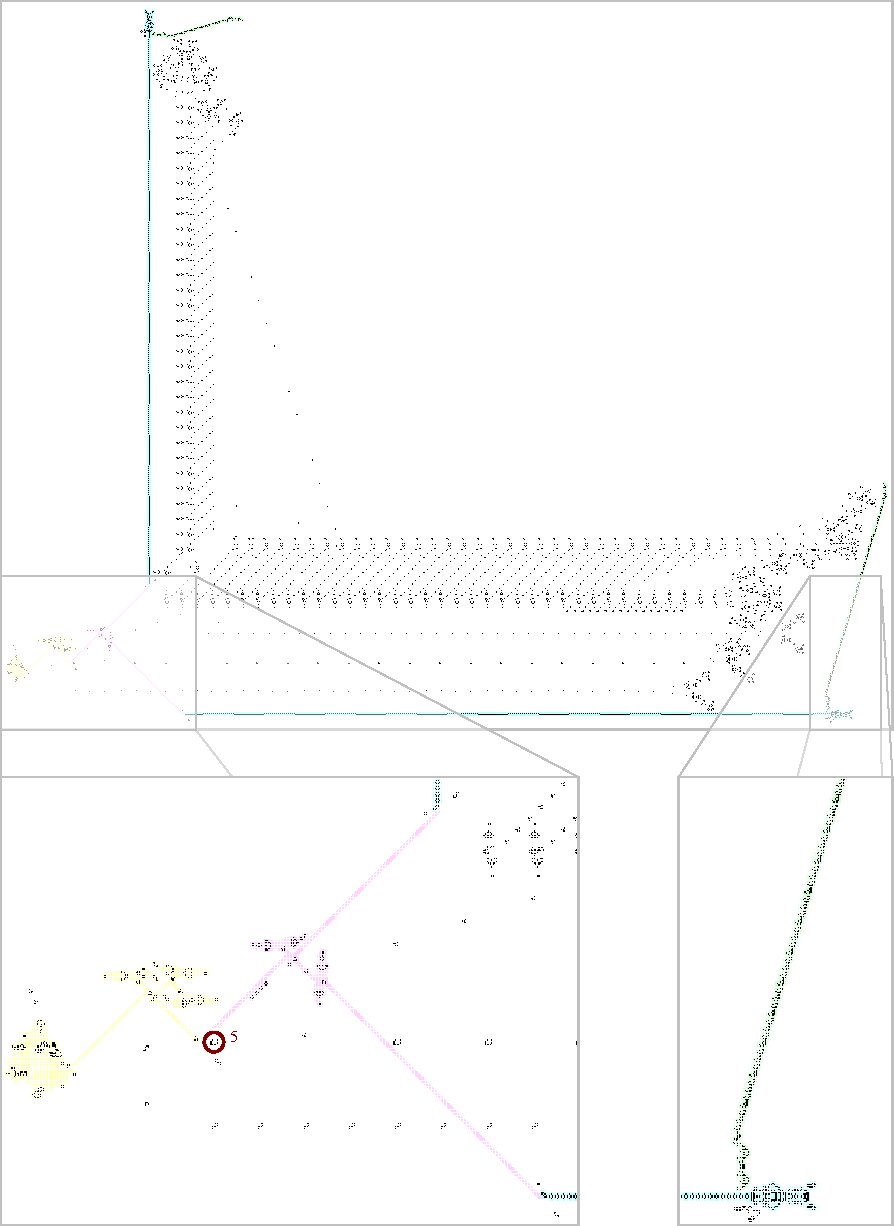
\includegraphics[width=\textwidth]{glider_guns/fermat_prime.pdf}}
	\caption{A Fermat prime calculator that self-destructs and has bounded population if a sixth Fermat prime exists, but grows without bound otherwise. A caber tosser (highlighted in \bgbox{yellowback2}{yellow}) fires gliders at the lightweight spaceships that the primer creates corresponding to integers of the form $2^n+1$ (the LWSS corresponding to the Fermat prime $5$ is circled in \bgbox{redback}{red}). If that LWSS is present (i.e., $2^n+1$ is prime) then the glider is reflected and destroys one of the four tubs to its northeast (they are destroyed by the known Fermat primes $5$, $17$, $257$, and $65{\thousep}537$). If another Fermat prime is found, the glider goes through a glider duplicator (highlighted in \bgbox{magentaback}{magenta}) and ignites two $4c/5$ beehive wicks that are laid by beehive puffers (highlighted in \bgbox{aquaback}{aqua}). Those wicks eventually cause two extensible $c/2$ spaceships (highlighted in \bgbox{greenpastel}{green}) to explode, blocking the primer.}\label{fig:fermat_primer}
\end{figure}

For spacing and timing reasons, this particular pattern starts with the Fermat prime $5$ (not $3$), and gliders corresponding to the Fermat primes $5$, $17$, $257$, and $65{\thousep}537$ each destroy a single tub near the southwest corner of the pattern. If a sixth Fermat prime is ever found, the resulting glider is fed into a glider duplicator that ignites both fuses and leads to the primer's self-destruction. However, such self-destruction will not happen until at least generation
\[
	120 \times 2^{2^{33}} \approx 1.16 \times 10^{2{\thousep}585{\thousep}827{\thousep}975},
\]
so evolving this pattern via computer software is not actually an effective method of checking whether or not a sixth Fermat prime exists.

While it is not possible to run this pattern long enough to see it self-destruct, we can force its self-destruction by manually erasing one or more of the glider-absorbing tubs at its southwest corner. If we erase all $4$ of those tubs, the glider corresponding to the Fermat prime $5$ almost immediately triggers the primer's self-destruction, whereas deleting a smaller number of tubs delays its self-destruction somewhat. If we remove just $1$ tub, the self-destruct fuse is ignited after roughly $8$~million generations (by the glider corresponding to the Fermat prime $65{\thousep}537$) and the primer finally stabilizes after roughly $21$~million generations.


%%%%%%%%%%%%%%%%%%%%%%%%%%%%%%%%
\section{Notes and Historical Remarks}\label{sec:glider_guns_history}
%%%%%%%%%%%%%%%%%%%%%%%%%%%%%%%%

Many of the ideas discussed early in this chapter were investigated right from the early days of Life. For example, many of the glider deletion tricks of Section~\ref{sec:glider_deletion} were already known in the early 1970s and were used to create the same period~$60$ gun that we constructed in Figure~\ref{fig:p60_gun}---see Figure~\ref{fig:lifeline_v11}. Indeed, the idea of encoding information in gliders and then using collisions between gliders to encode logical operations was already well-established at that time, and many useful interactions of this type were simply found by hand.

Other than guns resulting from these simple glider logic tricks though, not many new guns were found after the p$30$ Gosper glider gun and the p$46$ twin bees gun in the years following 1971. Bill Gosper made a p$1100$ gun sometime around 1984, Dean Hickerson constructed a p$94$ gun in 1990, Bill Gosper made a p$144$ gun in 1994 (see Exercise~\ref{exer:p144_gun_from_achim}), and David Buckingham had constructed guns of period~$44$ and $136+8n$ ($n \geq 1$), mostly based on his early work with Herschel tracks, by the early 1990s. However, progress in this area was relatively stagnant until he revealed Herschel track technology in full in 1996, and most of the earlier guns were so large and unwieldy that they were made almost instantly obsolete at that time.

After Herschel tracks hit the mainstream, which allowed for the systematic creation of glider guns of arbitrary large periods, a collaborative effort among many Life enthusiasts between then and 2003 (initiated by Dietrich Leithner and Peter Rott, and mainly led by Jason Summers and Karel Suhajda) produced explicit glider guns of all periods from $14$ to $1{\thousep}000$. The guns in this collection have since been shrunk down considerably via newer technology like Snarks and syringes, and at least a few of them are typically updated whenever a new sparky oscillator is discovered (as long as that oscillator can be used as a filter or reflector, anyway).\footnote{This collection of small glider guns is now being maintained by Chris Cain and Dave Greene. Links to the up-to-date version of the collection can be found at \httpsurl{conwaylife.com/wiki/Dieter_and_Peter's_glider_gun_collection}.}

\begin{figure}[!htb]
	\centering
	\begin{minipage}[b]{0.46\textwidth}
		\centering
		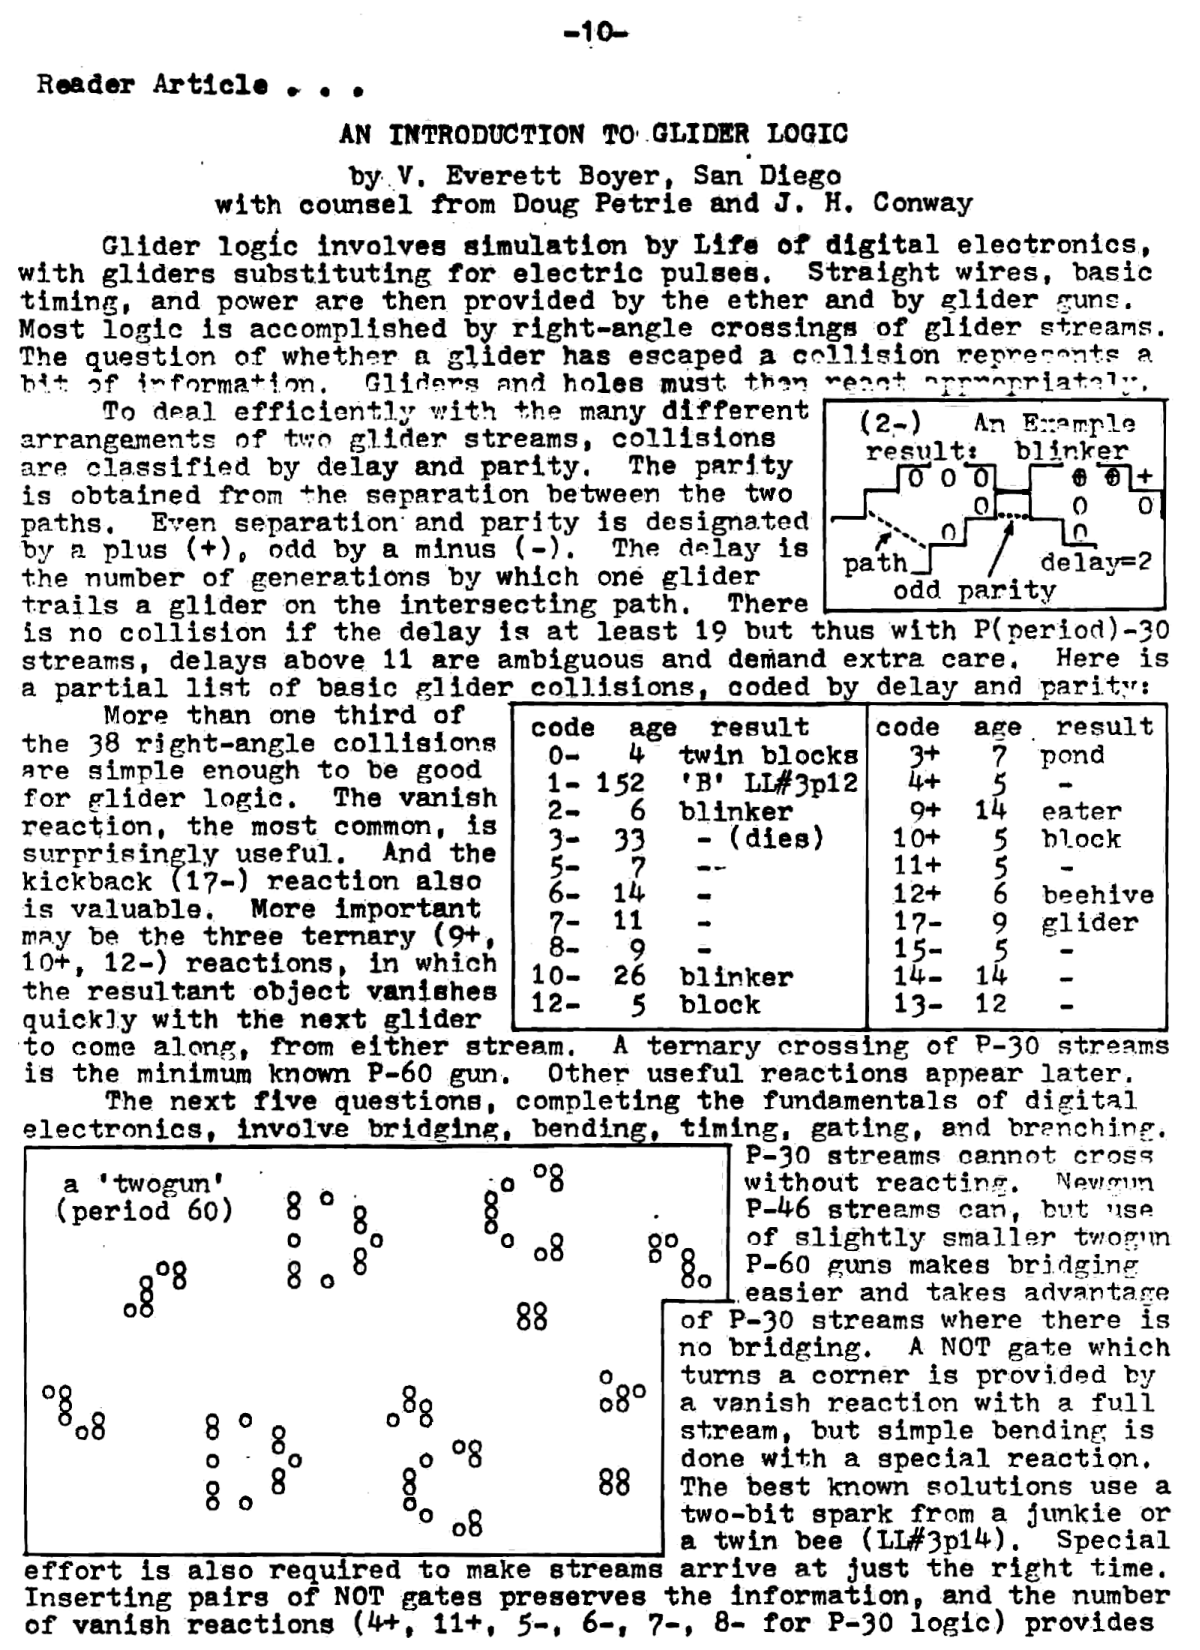
\includegraphics[width=0.8\textwidth]{glider_guns/lifeline_vol11.png}
		\caption{A page from the September 1973 issue (Volume 11) of \emph{Lifeline} that discussed glider logic and how it can be used to make a p$60$ glider gun (shown at the bottom left).}\label{fig:lifeline_v11}
	\end{minipage}\hfill
	\begin{minipage}[b]{0.5\textwidth}
		\centering
		\patternimglink{0.081}{p16_gun}
		\caption{A tightly-packed p$16$ glider gun that uses a p$48$ gun (highlighted in \bgbox{magentaback}{magenta}) and two p$48$ glider insertions (highlighted in \bgbox{aquaback}{aqua} and \bgbox{greenpastel}{green}).}\label{fig:p16_gun}
	\end{minipage}
\end{figure}

As a result of these repeated optimizations, most of the guns in this collection are now very cleverly and tightly packed---much moreso than the p$14$ gun that we constructed in Figure~\ref{fig:p14_gun}. Indeed, that gun had lots of empty whitespace that could be reduced by customizing the four glider insertion mechanisms that it uses, rather than using the exact same track for all four of them. For example, a particularly compact p$16$ gun is displayed in Figure~\ref{fig:p16_gun}.\footnote{However, this is not quite the smallest known p$16$ gun---see Exercise~\ref{exer:robs_p16_smaller_p16_gun}.} This gun uses a small p$24$ glider gun (one that is slightly smaller and newer than the one we saw in Figure~\ref{fig:p24_glider_gun}), which is then filtered to p$48$ by Rich's p$16$, and then sped up to p$16$ via two copies of the glider insertion reaction from Figure~\ref{fig:lwss_squish_pip}.

Patterns that decrease the asymptotic growth rate of a gun were known prior to the recursive filter of Figure~\ref{fig:recursive_filter}, but their effects were less pronounced. The first such pattern was a \emph{quadratic filter},\index{quadratic filter} which is displayed in Figure~\ref{fig:quadratic_filter}. This pattern produces its $n$-th output glider after receiving its $n(n+1)/2$-th input glider,\footnote{This device relies on p$90$ circuitry, so the input gliders have to be aligned to that period.} and thus decreases the growth rate of glider guns quadratically. In particular, appending this pattern to a gun whose population in generation~$t$ is $\Theta(f(t))$ results in a gun with whose population is $\Theta(\sqrt{f(t)})$. For example, if we append $n$ of these quadratic filters in series after a gun whose population grows linearly (i.e., a ``standard'' glider gun), we get a gun whose population is $\Theta(t^{1/2^n})$.

\begin{figure}[!htb]
	\centering
	\patternimglink{0.1425}{quadratic_filter}
	\caption{A \emph{quadratic filter}, which reduces the growth rate of a gun quadratically. It works by using a pair of gliders (highlighted in \bgbox{aquaback}{aqua}) to pull a block from an ever-receding trail (highlighted in \bgbox{greenpastel}{green}), similar to the loaf-pulling reaction used in the recursive filter of Figure~\ref{fig:recursive_filter}. The rest of the device (highlighted in \bgbox{magentaback}{magenta}) extends the back end of the block trail. Here, the filter is attached to a p$90$ glider gun (highlighted in \bgbox{yellowback2}{yellow}), resulting in a sqrtgun.\index{sqrtgun} Constructed by Gabriel Nivasch in June 2006.}\label{fig:quadratic_filter}
\end{figure}

The quadratic filter works by performing a block-pulling reaction whenever an input glider is received. Once a certain threshold is passed, the block is deleted, an output glider is released, and a farther-away block is created. If we rearrange the circuitry so that the location of the new block is pushed away \emph{every} time an input glider is received, rather than only when an output glider is produced, the filtering becomes even more pronounced. In fact, we get an \emph{exponential filter}---a\index{exponential filter} pattern that can be attached to the output of a glider gun so as to decrease its growth rate exponentially.

The particular exponential filter that is displayed in Figure~\ref{fig:exponential_filter} produces its $n$-th output glider after receiving $5 \times 2^n - 4$ input gliders, so appending it to a gun whose growth rate is $\Theta(f(t))$ results in a gun with the slower growth rate $\Theta(\log(f(t)))$. For example, feeding the output of a caber tosser into this exponential filter, as in Figure~\ref{fig:exponential_filter}, results in a gun whose population in generation~$t$ is $\Theta\big(\log(\log(t))\big)$.

\begin{figure}[!htb]
	\centering
	\patternimglink{0.136}{exponential_filter}
	\caption{An \emph{exponential filter}, which reduces the growth rate of a gun exponentially, attached to a caber tosser (highlighted in \bgbox{yellowback2}{yellow}) so that its population in generation~$t$ is $\Theta\big(\log(\log(t))\big)$. It works via most of the same mechanisms as the quadratic filter of Figure~\ref{fig:quadratic_filter}, and was also constructed by Gabriel Nivasch in June 2006.}\label{fig:exponential_filter}
\end{figure}

We could also apply several of these filters in sequence, producing guns with population
\[
	\Theta\big(\log(\log(\cdots (\log(t))))\big),
\]
where the logarithms are nested as many times as we like. However, even just a single usage of the recursive filter as in Figure~\ref{fig:recursive_filter_caber} results in a slower gun.


% EXERCISE: Make pattern with growth rate O(t^3/2) or O(t log^*t) (both easy, just attach guns we made here to a G-to-rake conduit). Earlier exercise: make G-to-rake conduit
% New p57: https://www.conwaylife.com/forums/viewtopic.php?f=2&t=3552&start=225#p128256
% Smallest p20 https://www.conwaylife.com/forums/viewtopic.php?p=85709#p85709

%%%%%%%%%%%%%%%%%%%%%%%%%%%%%%%%%
\section*{Exercises \hfill \normalfont\textsf{\small solutions to starred exercises on \hyperlink{solutions_glider_guns}{page \pageref{solutions_glider_guns}}}}
\label{sec:guns_exercises}
\addcontentsline{toc}{section}{Exercises}
\vspace*{-0.4cm}\hrulefill\vspace*{-0.3cm}\footnotesize\begin{multicols}{2}\vspace*{-0.4cm}\raggedcolumns\interlinepenalty=10000
	\setlength{\parskip}{0pt}
	%%%%%%%%%%%%%%%%%%%%%%%%%%%%%%%%%
	
	\begin{problemstar}\label{exer:p28_double} \probdiff{1}
		The glider collision in Figure~\ref{fig:glider_delete} can only be used to double the period of glider streams of period~$29$ or higher. Use the collision in Table~\ref{tab:2_glider_synth} that produces an eater~1 to double the period of a period~28 glider stream.
	\end{problemstar}

	
	\mfilbreak
	
	
	\begin{problem}\label{exer:gun_double_again} \probdiff{1}
		We used the reaction in Figure~\ref{fig:glider_delete} to turn two Gosper glider guns into a period~$60$ gun. Use that reaction multiple times to turn four Gosper glider guns into a period~$120$ gun.
	\end{problem}

	
	\mfilbreak
	
	
	\begin{problemstar}\label{exer:p322_gun} \probdiff{2}
		Use the reaction from Figure~\ref{fig:glider_delete6} to create a period~$322$ glider gun.
	\end{problemstar}
	
	
	\mfilbreak
	
	
	\begin{problem}\label{exer:duplicate_doubled_stream}
		The stream inverter-and-duplicator from Figure~\ref{fig:stream_inverter} is quite useful in situations where we want to duplicate a glider stream that took a lot of effort to create.\smallskip
		
		\begin{enumerate}[label=\bf\color{ocre}(\alph*)]
			\item \probdiff{1} Use three (not four!) Gosper glider guns and a single extra block to create a gun that fires two p$60$ streams of gliders.
			
			\item \probdiff{2} Use four (not six!) Gosper glider guns and two extra blocks to create a gun that fires three p$60$ streams of gliders.
		\end{enumerate}
	\end{problem}
	
	
	\mfilbreak
	
	
	\begin{problemstar}\label{exer:p80_gun_rich_p16} \probdiff{2}
		Use Rich's p16 (and potentially other sparkers as well) as a filter to turn the true-period~$20$ glider gun into a true-period~$80$ glider gun.
		
		\noindent [Hint: If you're lucky, you can get a single copy of Rich's p16 to delete \emph{two} consecutive gliders.]
	\end{problemstar}
	
	
	\mfilbreak
	
	
	\begin{problemstar}\label{exer:p4_glider_filter} \probdiff{2}
		We saw in Figure~\ref{fig:lwss_filter_tnosed_p4} that a filter can be used to double the period of any stream of lightweight spaceships with period $4n+2$ ($n \geq 3$). Explain why there cannot exist a filter capable of doubling the period of every stream of \emph{gliders} with period $4n+2$ ($n \geq 3$).
	\end{problemstar}


	\mfilbreak
	
	
	\begin{problem}\label{exer:p6_lwss_filter} \probdiff{2}
		Find an oscillator that can be used to double the period of any LWSS stream with period $6n+3$ ($n \geq 2$).
	\end{problem}
%	SOLUTION: p6 pipsquirter
%	x = 75, y = 20, rule = B3/S23
%	15bo2bo5b2o19bo2bo5b2o$b4o5b2o7bo3b4o4b4o5b2o7bo3b4o4b4o$o3bo3b2ob2o2b
%	o3bo3b2ob2o2bo3bo3b2ob2o2bo3bo3b2ob2o2bo3bo$4bo3b4o4b4o5b2o7bo3b4o4b4o
%	5b2o7bo$o2bo5b2o19bo2bo5b2o19bo2bo2$65bo$65bo2$63bo3bo$61b3obob3o$60bo
%	3b2o4bo$60bob2o2b2obobo$61bo2b2o2b2obo$62b2o2b2obobob2o$64bo2bobobob2o
%	$64b4ob2o$68bo$66bobo$66b2o!


	\mfilbreak
	
	
	\begin{problem}\label{exer:lwss_to_hwss_upgrade} \probdiff{2}
		We saw some ways of converting an LWSS into an MWSS and then an HWSS in Figure~\ref{fig:xwss_upgrade}. However, simpler conversions are possible with more loosely-packed streams.\smallskip
		
		\begin{enumerate}[label=\bf\color{ocre}(\alph*)]
			\item Find a way of colliding a single glider with the back end of a lightweight spaceship so as to convert it into a heavyweight spaceship.
			
			\item What periods of HWSS streams can be made via this reaction?
		\end{enumerate}
	\end{problem}


	\mfilbreak
	
	
	\begin{problem}\label{exer:pseudo_xwss_gun_p18} \probdiff{4}
		Recall the reactions from Figures~\ref{fig:lwss_insertion_p18} and~\ref{fig:xwss_upgrade} that can be used to create p18 xWSS streams.\smallskip
		
		\begin{enumerate}[label=\bf\color{ocre}(\alph*)]
			\item Use (potentially multiple copies of) the LWSS insertion reaction to create a p18 LWSS gun.
			
			\item Use the LWSS-to-MWSS reaction to turn your LWSS gun from part~(a) into a p18 MWSS gun.
			
			\item Use the MWSS-to-HWSS reaction to turn your MWSS gun from part~(b) into a p18 HWSS gun (which is the smallest period possible for such a gun!).
		\end{enumerate}
	\end{problem}
	
	
	\mfilbreak
	
	
	% SOLUTION: http://conwaylife.com/forums/viewtopic.php?f=2&t=1651&start=50#p18616
	% Smallest currently known, mention in solution
	\begin{problem}\label{exer:smaller_G_to_LWSS} \probdiff{4}
		The conduit from Figure~\ref{fig:H_plus_G_to_WSS} can be used to create smaller stable glider-to-LWSS and glider-to-MWSS converters than we have seen so far.\smallskip
		
		\begin{enumerate}[label=\bf\color{ocre}(\alph*)]
			\item Use that conduit to build a smaller stable glider-to-LWSS converter than the one that we constructed in Figure~\ref{fig:glider_to_lwss_both}(b).
			
			[Hint: Be careful---do not use periodic reflectors like we did in Figure~\ref{fig:H_plus_G_to_WSS}, and make sure that the glider collides with the \emph{same} Herschel, rather than the \emph{next} one like in that figure.]
			
			\item Use that conduit to build a stable glider-to-MWSS converter.
		\end{enumerate}
	\end{problem}
	
	
	\mfilbreak
	
	
	\begin{problem}\label{exer:p28_adjust_29} \probdiff{3}
		Adjust the reflectors in the gun from Figure~\ref{fig:p14_pieces_p84} to create a gun that emits $2$ out of $3$ gliders in a p$29$ (instead of p$28$) stream.
	\end{problem}
	
	
	\mfilbreak
	
	
	\begin{problem}\label{exer:p156_adjust_lwss} \probdiff{2}
		Adjust the reflectors reaction from Figure~\ref{fig:p14_pieces_lwss} to make it work with Herschel streams of period~$180$ (instead of~$156$).
	\end{problem}
	
	
	\mfilbreak
	
	
	\begin{problem}\label{exer:jasons_p36_caterer} \probdiff{2}
		Show how to stabilize Jason's p$36$ (see Figure~\ref{fig:jasons_p36}) with caterers instead of jams.
	\end{problem}
	% SOLUTION:
	%x = 39, y = 22, rule = B3/S23
	%26bo$25bobo2$2o23bo$bo23b2o$bobo18b5o$2b2o18b2ob2o$14b2o9bo$13b2o$14b
	%2o$15bo$23bo$23b2o$24b2o$13bo9b2o$12b2ob2o18b2o$12b5o18bobo$12b2o23bo$
	%13bo23b2o2$11bobo$12bo!
	
	
	\mfilbreak
	
	
	\begin{problem}\label{exer:p56_gun_smaller} \probdiff{2}
		Construct a true-period 56 gun that is smaller than the one from Figure~\ref{fig:p56_gun}.
		
		\noindent [Hint: Just add a filter to some other gun.]
	\end{problem}
	% SOLUTION: Filter the p28 gun with a blocker.
	
	
	\mfilbreak
	
	
	\begin{problem}\label{exer:smaller_p14_gun} \probdiff{4}
		By using (multiple copies of) the p28 glider gun from Figure~\ref{fig:p28_glider_gun}, construct a period~14 glider gun that is smaller than the one that we built in Figure~\ref{fig:p14_gun}.
	\end{problem}
	% SOLUTION: Posts right after https://www.conwaylife.com/forums/viewtopic.php?t=&p=115869#p115869
	
	
	\mfilbreak
	
	
	\begin{problem}\label{exer:p50_triple_gun} \probdiff{2}
		The true-period~$50$ glider gun in Figure~\ref{fig:true_p50_glider_gun} uses two copies of the central pi-heptomino reaction. Create a true-period~$50$ glider gun that uses three copies of that reaction.
	\end{problem}
	
	
	\mfilbreak
	
	
	\begin{problemstar}\label{exer:p50_glider_stabilize} \probdiff{3}
		Another method of stabilizing one side of the p$50$ pi-heptomino reaction used in the true-period~$50$ glider gun is displayed below.
		\begin{center}
			\patternimglink{0.1}{exer_p50_glider_stabilize}
		\end{center}
		\noindent Use this reaction to create a true-period~$50$ glider gun with a lower population than the one displayed in Figure~\ref{fig:true_p50_glider_gun}. In particular, use two mirror-image copies of the glider-extracting conduit and then feed one of those gliders back into the reaction via...\smallskip
		
		\begin{enumerate}[label=\bf\color{ocre}(\alph*)]
			\item two Snarks.
			
			\item two bumpers (what is the only known bumper period that works with period~$50$ mechanisms?).
		\end{enumerate}
	\end{problemstar}
	
	
	\mfilbreak
	
	
	\begin{problem}\label{exer:fx77_extract_other_osc} \probdiff{2}
		Show how to extract a glider from an Fx77 conduit like we did in Figure~\ref{fig:fx77_extract} via the following oscillators:\smallskip
		
		\begin{enumerate}[label=\bf\color{ocre}(\alph*)]
			\item a unix (p$6$),
			
			\item a pentadecathlon (p$15$), and
			
			\item Beluchenko's p$7$ (Figure~\ref{fig:sparky_p7}).
		\end{enumerate}
	\end{problem}
	% SOLUTION: https://conwaylife.com/wiki/Fx77
	
	
	\mfilbreak
	
	
	\begin{problem}\label{exer:p54_fold_corners} \probdiff{3}
		The p$56$ glider gun displayed in Figure~\ref{fig:p56_gun} uses three reflectors at its top and at its bottom, instead of just one, to make it bounding box slightly smaller. You can similarly ``fold in'' the top and bottom corners of some other guns to make their bounding boxes smaller.
		
		\begin{enumerate}[label=\bf\color{ocre}(\alph*)]
			\item Modify the p$54$ glider gun from Figure~\ref{fig:p54_gun} so that its bounding box has at at least $300$ fewer cells in it.
			
			\item Modify the p$55$ glider gun from Figure~\ref{fig:p55_gun} so that its bounding box has at at least $700$ fewer cells in it.
		\end{enumerate}
	\end{problem}
	
	
	\mfilbreak
	
	
	\begin{problem}\label{exer:H_G_reacs_58_61} \probdiff{1}
		Determine the repeat times of the four conduits from Figure~\ref{fig:H_G_reacs_58_61}.
	\end{problem}
	
	
	\mfilbreak
	
	
	\begin{problem}\label{exer:p61_gun_reflection_no_60} \probdiff{2}
		Explain why the method of separating the two close glider streams in the p$61$ gun from Figure~\ref{fig:p61_gun} (by reflecting one of the gliders off of the corner of an L112 conduit) does not work at p$58$, p$59$, or p$60$, despite L112 having a repeat time of~$58$ generations.
	\end{problem}
	% SOLUTION: eater 2 only fast enough at p61 and higher. Can replace with another eater (to get lower repeat time, like eater 5 variant), but then interferes with passing gliders
	
	
	\mfilbreak
	
	
	\begin{problem}\label{exer:2_lane_slide_gun} \probdiff{3}
		Use the reaction from Figure~\ref{fig:synchronized_block_reflector_4} to create a slide gun that fires gliders separated by $2$ lanes (instead of $4$ lanes, like the slide gun from Figure~\ref{fig:slide_gun}).
	\end{problem}
	
	
	\mfilbreak
	
	
	\begin{problem}\label{exer:slide_gun_honey_farm}\index{honey!farm} \probdiff{4}
		Slide guns can be made to work by pushing any stable object, not just a block. Use the following reactions\footnote{Both found by Jason Summers in 1999. The reaction in part~(a) was used in the quadratic and exponential filters of Figures~\ref{fig:quadratic_filter} and~\ref{fig:exponential_filter}.} to create slide guns:\\[0.05cm]
		
		\begin{enumerate}[label=\bf\color{ocre}(\alph*)]
			\item \raisebox{-\height+\ht\strutbox}{\patternlink{exercise_honey_farm_pusher}{\vcenteredhbox{\patternimg{0.1}{exercise_honey_farm_pusher_0}} \vcenteredhbox{\genarrow{51}} \vcenteredhbox{\patternimg{0.1}{exercise_honey_farm_pusher_1}}}}\\[0.1cm]
			
			\item \raisebox{-\height+\ht\strutbox}{\patternlink{exercise_beehive_pusher}{\vcenteredhbox{\patternimg{0.1}{exercise_beehive_pusher_0}} \vcenteredhbox{\genarrow{33}} \vcenteredhbox{\patternimg{0.1}{exercise_beehive_pusher_1}}}}\\[0.1cm]
		\end{enumerate}
	\end{problem}
	% SOLUTION FOR (a) is contained in here:
	%x = 263, y = 178, rule = B3/S23
	%186bo2b2o$186bo2bo$186bo11$168b2o$169b2o$168bo3$163b2o$164b2o22bo$163b
	%o25bo$187b3o$177b3o$179bo$178bo12$145b2o$146b2o$145bo3$140b2o$141b2o$
	%140bo2$154b3o$156bo$155bo$211bo$212bo$210b3o9$122b2o$123b2o$122bo2$
	%188b2o$117b2o69bo$118b2o$117bo2$131b3o$133bo6b2o$132bo7bo$77b2o$77bo4$
	%244bo$29b2o211b2o$29bo41bo5bo165b2o$70b3o3b3o109bo7bo$69b2o2bobo2b2o
	%107b4o3b4o$69bo3bobo3bo107bo3bobo3bo$69bob2o3b2obo19b2o41b2ob2o41bo2bo
	%bo2bo$69b2o7b2o20b2o40b2ob2o41b3o3b3o$99bo42b2ob2o$140bob2ob2obo$140b
	%3o3b3o$22b3o3b3o63b2o45bo5bo$22bo2bobo2bo64b2o$22bo7bo63bo$195b2o9bo2b
	%2o$108b3o62bo21bo10bo2bo$110bo58b2o2bo32bo$109bo58bo5bo$167b2o2bobo$
	%168b2o3bo$169b3o2$77b2o90b3o$77bo59b3o3b3o22b2o3bo$58b2o3bo73bo2bobo2b
	%o15b2o4b2o2bobo$58b3obob2o71bo7bo5bo9bo6bo5bo$58b3o4bo86b2o15b2o2bo$
	%61bo3bo85b2o20bo14b2o$27bobo32b3o3bo120b2o$28b2o38b2o6b2o110bo$28bo33b
	%3o3b2o7b2o127b2o$61bo3bo10bo130b2o$43b2o13b3o4bo117b2o21bo$43bo14b3obo
	%b2o118b2o$58b2o3bo7b2o110bo$72b2o$71bo125b3o$199bo$18b2obo3bob2o56b3o
	%47b2o17b2o42bo$19b3o3b3o11bo47bo48bo17bo$20bo5bo13b2o44bo46b3o19b3o$
	%39b2o92bo23bo5$17b2o17b2o$18bo17bo$15b3o19b3o134bo$15bo23bo135b2o$23b
	%3o3b3o108b2obo3bob2o23b2o37bo$22bo2bo3bo2bo108b3o3b3o62b2o$22b2obo3bob
	%2o56bo52bo5bo63bobo$88b2o$88bobo102b2o$160b2o29b2ob2o14b2o$161b2o28bo
	%2bo15bo$48b2o110bo30bo2bo$49b2o141b2o$48bo$148b2o15b2o25b2o$62b3o83bo
	%16bo25bo2bo$64bo16b4o78bobo17b2o6bo2bo15b2o2b2o$63bo17bo2b2o6b2o69b2o
	%18bo7b2ob2o14bo4bo7b2obo$82bo2b2o5bo100b2o20bobo4bob2ob2o$82bo2bo73b2o
	%55b2o4bo3b2o$83b2o74bo64bo$170b2o51b2o$30b2o15b2o34b2o84bo2b2o11b2o20b
	%2o$30bo16bo34bo2bo32b2o9b4o35b6o11bo23bo$38b2o5bobo17b2o15bo2b2o31bo
	%10b2obo37b4o20b2o10b2o2bo35b3o$38bo6b2o18bo15bo2b2o46bo20b2o39bo12bo2b
	%o33bo4bo11b2o$81b4o45b2o20bo2bo52bobo18bo14bo5bo10bo$151b2o2bo52b2o18b
	%2o6bo12bo$130b2o20bo2bo14b4o53b3obo3b2o10b2o$54b3o55bo19bo20bo14b6o34b
	%2o16b2o7bobo$15b2o36bo4bo8b2o42b2o16b2obo36bo2b2o34bobo16b2o18b2o$14bo
	%2bo34bo5bo8bo35b2o6bobo15b4o20bo16b2o35bo2bo17bo20bo$13b2o2bo35bo50bo
	%47bo2bo50b2o2bo33bo5bo$14bo2bo14b2o20b2o48bobo44b2o2bo53bo18bo15bo4bo$
	%15bo9b2o4bo2b2o69b2o45bo2bo51b2o18b2o17b3o$26b2o2b6o18b2o97b2o8b2o61b
	%2o$15bo9bo6b4o17bo109bobo61b3obo$14bo2bo34bo5bo106bo50b2o10b2o$2o11b2o
	%2bo35bo4bo41b2o63b2o48bobo11bo$o13bo2bo36b3o26b2o15bobo112bo$15b2o15b
	%4o47bo18bo36b3o8b2o62b2o$30b6o64b3o20b2o16bo8bo$31bo2b2o78bo7b2o17bo$
	%32b2o11b2o66b2o9bo15bo$45bobo64b2o$47bo52b3o10b2o25bo$47b2o53bo38bo$
	%100bobo38bo$100b2o37b3o$113b2o$112b2o$113b2o$105b2o7bo$104bobo$104bo$
	%103b2o!
	% SOLUTION FOR (b) -- should probably be rebuilt using an MWSS-creating mechanism we have actually seen before:
	%x = 124, y = 91, rule = B3/S23
	%101b2o14b2o$101b2o14b2o5$100b3o$100b3o$99bo3bo2$98b2o3b2o12b3o$116bo3b
	%o$115bo5bo$115bo5bo$118bo$98b3o15bo3bo$40b2o60b2o13b3o$39bobo60b2o14bo
	%$29b2o7b3o12bo49b2o$29b2o6b3o8b2o3b4o44bobo$38b3o8b2o3b4o5b2o36b2o16b
	%3o$39bobo2b2obob2o3bo2bo5b2o54b3o$40b2o2b2obobo4b4o60bo3bo$23bo22b2obo
	%3b4o39b2o3b2o9bobo$21bobo29bo42b2o3b2o9b2o3b2o3b2o$12bo7bobo11b2o77bo$
	%11b2o6bo2bo11b2o62b3o$10b2o4b2o2bobo16bo58b3o$2o7b3o4b2o3bobo13b2o60bo
	%$2o8b2o4b2o5bo14b2o$11b2o73bo$12bo73bo$24bo60bobo$25bo60bo9b2o$23b3o
	%60bo10bo21b2o$30bobo53bo7b3o22b2o$29b3o54bo7bo$27b5o53bobo$27bobo56bo
	%10bobo$29bo56bo10b2o$29b2o67bo$110bo$108bo3bo3b2o$25bo11bo29bo29bo15bo
	%bo2bo$24bobo8bo3bo25bo3bo25bo3bo8bo4bo2b2o$23bo3bo12bo29bo29bo8b5o$23b
	%o3bo7bo4bo24bo4bo24bo4bo$23bo3bo8b5o25b5o13b2o10b5o$23bo3bo57b2o$23bo
	%3bo56bo$23bo3bo8b2o$24bobo40bo$25bo9bo12bo16b3o$36bo8b4o15bo$32b2o10b
	%4o9b2o5b2o19bo$32bobo9bo2bo9b2o24b3o$33b3o8b4o5bo28bo$34b3o8b4o4bo28b
	%2o$33b3o12bo$25b2o5bobo44bo$24bobo5b2o45bo$24bo55bo$23b2o44b2o$70b2o$
	%60b5o4bo7b2o3b2o$59bob3obo11bo5bo$60bo3bo$61b3o10b2o2bo3bo$62bo10b2o4b
	%3o$63b2o10bo$63bobo$63bobo$64bo3$61b2obob2o10bo$61bo5bo8b2ob2o$62bo3bo
	%$63b3o9bo5bo2$75b2obob2o6$64b2o$64b2o2$77b2o$77b2o!
	
	
	\mfilbreak
	
	
	\begin{problem}\label{exer:simkin_glider_gun_smaller_slide} \probdiff{3}
		Use the small p$120$ glider gun from Exercise~\ref{exer:simkin_glider_gun} to rebuild the slide gun from Figure~\ref{fig:slide_gun} within an $85 \times 70$ bounding box.
	\end{problem}
	% SOLUTION
	%x = 64, y = 80, rule = B3/S23
	%52bo$50b3o$8b2o39bo$8b2o39b2o3$11b2o$11b2o31b3o$46bo6b2o5b2o$8b2o35bo
	%7b2o5b2o$8b2o$2o33bo20b2o$bo32bobobo17b2o$bobo32bo2bo$2b2o$35bo$35bo$
	%35b2o$9bo2bo22bo3bo$7b4o18b2o4bob2o$13bo15b2o4b3o$7b2o2b2o2$11b2o$12b
	%2o$8bo2b2o$19b2o$19b2o10bo$29bobo$16b2o12b2o$16b2o7bo$25b3o$28bo12b2o$
	%19b2o6b2o13bo$19b2o21bobo7bo$43b2o5bobo$33bobo12b2o$34b2o12b2o12b2o$
	%34bo13b2o12b2o$50bobo$30bo21bo$29b3o9bo$28b5o8b2o$27b2o3b2o6bobo3$31bo
	%$19b2o10bo$19b2o$27b2o$28bo$16b2o7b3o$16b2o7bo2$19b2o$19b2o3$59b2o$59b
	%2o2$20bo$17b5o$16bo2$17bo3bo$18b3o$2b2o$bobo$bo$2o$8b2o$8b2o2$11b2o$
	%11b2o3$8b2o$8b2o!
	
	
	\mfilbreak
	
	
	\begin{problem}\label{exer:edge_shoot_30n}
		The device below\footnote{Found by Arie Paap and Tanner Jacobi in late 2018 in a period~$30n$ ($n \geq 2$) form, and adjusted to the period~$5n$ form shown here in late 2019.} can be attached to the output of any gun with period~$5n$ ($n \geq 8$) to create an edge-shooting gun of the same period:
		\begin{center}
			\patternimglink{0.12}{exercise_edge_shoot_30n}
		\end{center}
		
		\begin{enumerate}[label=\bf\color{ocre}(\alph*)]
			\item \probdiff{3} Use this reaction to create an edge-shooting p$240$ gun.
			
			\item \probdiff{4} Use $10$ copies of the gun from part~(a) (and perhaps the p$120$ glider gun from Exercise~\ref{exer:simkin_glider_gun}) to rebuild the slide gun from Figure~\ref{fig:double_slide_gun} in a much smaller way. In particular, this edge shooter lets you avoid using the glider insertion mechanism from Figure~\ref{fig:lwss_reflect_glider}.
		\end{enumerate}
	\end{problem}
	
	
	\mfilbreak
	
	
	\begin{problem}\label{exer:slide_gun_hd} \probdiff{4}
		Create a slide gun that fires gliders separated by just $1$ lane.
		
		\noindent [Hint: This is tricky! The reactions like Figure~\ref{fig:synchronized_block_reflector_4} that move a block $1$~cell diagonally result in slide guns with a separation of $2$~lanes.]
	\end{problem}
	% Solution: need 2 separate firing reactions. Fire, then move by (0,1), then fire, then move by (1,0), repeat
	
	
	\mfilbreak
	
	
	\begin{problem}\label{exer:slide_gun_no_slide} \probdiff{2}
		Create a ``slide'' gun that fires $7$~gliders at a block so as to create a perpendicular glider without moving the block at all. That is, create a slide gun that doesn't slide.
	\end{problem}
	% SOLUTION: just remove 3 gliders from {fig:double_slide_gun}
	
	
	\mfilbreak
	
	
	\begin{problem}\label{exer:triple_slide_gun} \probdiff{4}
		Create a slide gun that fires $3$~gliders on each of its output lanes (instead of $2$, like in Figure~\ref{fig:double_slide_gun}).
		
		\noindent [Hint: Using an edge-shooting gun like the one from Exercise~\ref{exer:edge_shoot_30n} will help keep the size of your slide gun down.]
	\end{problem}


	\mfilbreak
	
	
	\begin{problem}\label{exer:four_lane_gun_smaller} \probdiff{3}
		Decrease the bounding box of the four-lane gun from Figure~\ref{fig:armless_4_lane_gun} so that it no larger than $275 \times 275$, by using Snarks to wrap the glider loops around like we did in Figures~\ref{fig:armless_monochrome_cordership_gun} and~\ref{fig:armless_cordership_gun}.
	\end{problem}
	% SOLUTION: https://conwaylife.com/forums/viewtopic.php?p=85842#p85842
	
	
	\mfilbreak
	
	
	\begin{problem}\label{exer:armless_basics}
		Armless glider production is a useful and highly adjustable mechanism, but some adjustments have consequences that may not be intuitively obvious.\smallskip
		
		\begin{enumerate}[label=\bf\color{ocre}(\alph*)]
			\item \probdiff{2} What behavior appears if you try to produce perpendicular output gliders via two loop guns whose periods differ by a multiple of 8?
			% SOLUTION: the output glider lane(s) drift in one direction or the other, eventually reaching and probably destroying one of the loop guns.
			
			\item \probdiff{4} Make a design for a ``drifting'' armless gun that would allow loop guns of different periods, but avoid the problem that was alluded to in part~(a).
			% SOLUTION: One option would be to adjust the loop guns' periods to particular multiples of 8, so that there's some number P = N*{gun1 period} = (N+1)*{gun2 period}. Then add an additional period-P gun that suppresses one signal from gun #2, producing a period-P ``scanning'' or ``strobing'' effect.
		\end{enumerate}
	\end{problem}
	
	
	\mfilbreak
	
	
	\begin{problem}\label{exer:armless_tee}
		In Section~\ref{sec:armless}, we only constructed armless guns that fire slow salvos. However, we can also construct ones that fire synchronized salvos.\smallskip
		
		\begin{enumerate}[label=\bf\color{ocre}(\alph*)]
			\item \probdiff{4} Use (several copies of) the p387 loop gun displayed below on the left, along with the H-to-2G conduit that we used in our tee-based armless guns, to create a $4$-consecutive-lane armless gun that fires the tight arrangement of gliders displayed below on the right.\\[-0.6cm]
			
			\begin{center}
				\begin{minipage}[t]{.575\linewidth}\vspace{0pt}
					\centering \patternimglink{0.1}{exercise_herschel_tee_387_loop}
				\end{minipage} \hfill %
				\begin{minipage}[t]{.38\linewidth}\vspace{0pt}
					\centering \patternimglink{0.14}{exercise_herschel_tee_4_gliders}
				\end{minipage}
			\end{center}
		
			\item \probdiff{2} Adjust your gun from part~(a) so that it fires that configuration of gliders with period 129.
			
			\noindent [Hint: $129 \times 3 = 387$.]
			
			\item \probdiff{3} Adjust your gun from part~(a) so that it fires that configuration of gliders with period 87 (which is minimal).
			
			\noindent [Hint: $387+6 \times 8 = 435 = 87\times5$, so first adjust each loop to be 6fd bigger.]
		\end{enumerate}
	\end{problem}
	% SOLUTIONS: patterns are posted at  https://conwaylife.com/forums/viewtopic.php?p=86064#p86064


	\mfilbreak


	\begin{problem}\label{exer:armless_tee_decrease_repeat_time}
		In this exercise, we explore some methods that can be used to decrease the repeat time of an armless gun.\smallskip
		
		\begin{enumerate}[label=\bf\color{ocre}(\alph*)]
			\item \probdiff{3} The tee-based armless Cordership gun of Figure~\ref{fig:armless_monochrome_cordership_gun} has already been adjusted to close to its recipe's minimum repeat time of $2{\thousep}061$ generations. Explain how additional loop guns could be added to allow a repeat time of less than $2{\thousep}000$ generations.
			% SOLUTION: Add more loop guns: Wherever a 74-tick limitation appears, move one of the gliders involved to a separate pair of loop guns.
			
			\item \probdiff{5} How could the repeat time of this gun be reduced \emph{without} increasing the number of loop guns?
			% SOLUTION: There are some long stretches of same-color gliders in both salvos making up the Cordership glider-pair recipe. For the glider pairs that build blocks, there are alternate recipes (e.g., the mirror image of the current recipe) that can switch one or both gliders to a different color.
			%Might not need a figure for this, but here's some RLE just in case. The left-side glider is a different color in these two recipes:
			% x = 34, y = 9, rule = LifeHistory
			% 4.2D23.2D$3.B2DB22.2DB$2.5B22.2B2C$.4B.3B18.4BCBC$3CB2.4B16.4B.CB$2BC
			% 4.4B14.2C3B$.C6.2B2C12.CBCB$9.BCBC12.BC$10.CB!
			% ... and if you take the mirror image of the right-side recipe, both gliders change colors.
		\end{enumerate}
	\end{problem}
	
	
	\mfilbreak
	
	
	\begin{problem}\label{exer:slow_glider_pairs_cordership_armless}
		In a tee-based armless gun that implements 2-directional slow synthesis, the gliders in the loop guns are synchronized in groups of four. Adjustments to the four gliders in a group can make a collision happen in a different place, or at a different time.\smallskip
		
		\begin{enumerate}[label=\bf\color{ocre}(\alph*)]
			\item \probdiff{2} Find a case where a glider follows another one by just 74 generations in the tee-based armless Cordership gun of Figure~\ref{fig:armless_monochrome_cordership_gun}. Then find the other three gliders that are synchronized with that glider, and delay all four gliders by one generation. What happens?
			% SOLUTION: Most likely the recipe will still work, but one part of it will be constructed one tick more slowly than before. Occasionally, if the changed position causes a conflict with other gliders, the recipe will fail.
			
			\item \probdiff{2} Return the four gliders to their original positions, and instead of delaying them all, advance them all by one generation. What happens?
			% SOLUTION: The other three gliders in the group will generally have much plenty of space in front of them, but the first glider's 74-tick spacing is a limiting factor that prevents that particular collision from occurring any sooner in the construction recipe. Attempting to advance the 74-tick following glider will cause a failure in the syringe conduit, the next time that glider attempts to pass through.
			
			\item \probdiff{3} Find the four gliders that collaborate to produce the southernmost block in the Cordership seed. How would you move those gliders to build the block two cells directly south of its current position, or one cell directly southeast or southwest?
		\end{enumerate}
	\end{problem}


	\mfilbreak
	
	
	\begin{problem}\label{exer:multicolor_armless}\index{NW31}
		It is somewhat easier to change the period of a multicolor armless gun than the monochrome one, since they have fewer glider loops to adjust. The multicolor armless Cordership gun of Figure~\ref{fig:armless_cordership_gun} has period $5{\thousep}603$.\smallskip
		
		\begin{enumerate}[label=\bf\color{ocre}(\alph*)]
			\item \probdiff{3} A syringe followed by NW31 (i.e., the conduit of Figure~\ref{fig:H_to_2G}) makes a stable glider reflector. Add one of these reflectors to one of the loop guns from the multicolor armless Cordership gun. How does its period change?
			
			\noindent [Hint: Start by moving some Snarks a long distance away to make space.]
			% SOLUTION: adding a syringe+NW31 component similar to the ones in the Cordership guns, will add 3 ticks (mod 8) to the period.  That is, if the gun period is N before adding a syringe+NW31, then after the addition it will be possible to adjust the new period to N+3.
			
			\item \probdiff{3} Adjust that glider loop so that it has period $2^{13} = 8{\thousep}192$.
			
			[Hint: You cannot just adjust the trombone slides, since the mod-$8$ length of that loop is not right. Either add more syringe $+$ NW31s or add another reflector from Table~\ref{tab:conduit_phase_changers}.]
			% SOLUTION: a chain of seven syringe+NW31s will allow for a p2603+7*3+8N gun, which can be adjusted to period 8192.
			
			\item \probdiff{4} Make the same adjustments to the other three loop guns to produce a working period~$8{\thousep}192$ Cordership gun.
		\end{enumerate}
	\end{problem}
	
	
	\mfilbreak
	
	
	\begin{problem}\label{exer:caber_tosser_rewind} \probdiff{2}
		Explain why we cannot rewind the caber tosser from Figure~\ref{fig:caber_tosser_0} so that the triggering glider in aqua is traveling northwest before it is reflected by the caber tosser.
	\end{problem}
	
	
	\mfilbreak
	
	
	\begin{problem}\label{exer:caber_tosser_stationary} \probdiff{3}
		Construct a caber tosser that uses the same Cordership and glider bouncing off of it as in Figure~\ref{fig:caber_tosser_0}, but uses stationary circuitry (e.g., syringes and Herschel conduits) in place of the glider guns.
	\end{problem}
	
	
	\mfilbreak
	
	
	\begin{problem}\label{exer:caber_tosser_different_speeds} \probdiff{2}
		If a caber tosser makes use of a receding spaceship with speed $s_1$ (instead of a Cordership) and bouncing spaceship with speed $s_2$ (instead of a glider), what is the ratio of the gaps between the gliders that it emits? For example, in the caber tosser of Figure~\ref{fig:caber_tosser_0} we had $s_1 = c/12$, $s_2 = c/4$, and a ratio of $2$ (each glider took twice as long to be emitted as the previous one).
	\end{problem}
	% SOLUTION: $(s_2+s_1)/(s_2-s_1)$
	
	
	\mfilbreak
	
	
	\begin{problem}\label{exer:sqrtgun_standard} \probdiff{4}
		Rebuild the sqrtgun from Figure~\ref{fig:sqrtgun} without any Herschel tranceivers---use syringes (and other ``modern'' Herschel conduits) instead.
	\end{problem}
	
	
	\mfilbreak
	
	
	\begin{problem}\label{exer:construct_fermat_primer} \probdiff{2}
		Construct a gun that emits lightweight spaceships corresponding to Fermat primes (much like the primer itself emits lightweight spaceships corresponding to all primes), rather than a pattern that self-destructs if it finds a sixth Fermat prime like the one we made in Figure~\ref{fig:fermat_primer}.
	\end{problem}
	
	
	\mfilbreak
	
	
	\begin{problem}\label{exer:fermat_beehive_puffer} \probdiff{2}
		The beehive puffer that is used at the bottom-right and top-left of the Fermat prime calculator (see Figure~\ref{fig:fermat_primer}) is displayed below.
		
		\begin{center}
			\patternimglink{0.1}{fermat_beehive_puffer}
		\end{center}
		
		\noindent This puffer still works even if the cells highlighted in \bgbox{aquaback}{aqua} are deleted. What is their purpose in the Fermat prime calculator?
	\end{problem}


	\mfilbreak
	
	
	\begin{problem}\label{exer:mersenne_primer}\index{Mersenne prime} \probdiff{3}
		Modify the Fermat prime calculator of Figure~\ref{fig:fermat_primer} so that it computes \textbf{Mersenne primes}: primes of the form $2^n - 1$ for some integer $n$.
	\end{problem}
	% SOLUTION: Example solution given here: http://www.njohnston.ca/2009/08/generating-sequences-of-primes-in-conways-game-of-life/
	% http://www.conwaylife.com/patterns/mersenneprimecalculator.rle
	
	
	\mfilbreak
	
	
	\begin{problem}\label{exer:robs_p16_smaller_p16_gun}
		Recall the small p$16$ oscillator from Figure~\ref{fig:rob_p16} called Rob's p$16$.\smallskip
		
		\begin{enumerate}[label=\bf\color{ocre}(\alph*)]
			\item \probdiff{2} Show how Rob's p16 can be used to filter a p$24$ LWSS stream, creating a p$48$ stream.
			
			\item \probdiff{2} What LWSS stream periods can be filtered by Rob's p16? % $16n+8$ for any $n \geq 1$ (same as Rich's p16)
			
			\item \probdiff{4} Use the filtering reaction from part~(a) to reduce the bounding box of the p$16$ glider gun that we saw in Figure~\ref{fig:p16_gun} by at least $2$ rows or columns.
		\end{enumerate}
	\end{problem}
	% SOLUTION:
	%x = 156, y = 154, rule = B3/S23
	%5b2ob2o5bo3bo5b2ob2o63b2o$5b2obo5b2o3b2o5bob2o61b3obo19b2o4b2o3b2o4b2o
	%b2o$8bob2o11b2obo63bo4bo12b2o5bobo3b2o3b2o3bobob2o$8bo6b2ob2o6bo62bobo
	%bob2o10bo2bob2obo5bobobobo5bo$9b2o13b2o55b2o7bo2bo13bo2bobo2bo2bo11bo
	%2bo$3bobo6bo2b2ob2o2bo27b2o28bo2bo2b4o2b2ob2o3b2o2b2ob4o2bo2bo15bo$b3o
	%b3o5b3o3b3o27bob3o20b2o4b3o2b7obobo4b2o2bobo4b2o7bob2ob2obo7bobo$o7bo
	%5bo5bo8bo19bobo2bo19bo8b9o3bo10bob2o10bo2bobo2bo5b3ob3o$ob6o20bobo4bo
	%12b2o2b2obo20bo5bo10b2o3b4o3bob2ob3o7b3o3b3o4bo7bo$7bo20bobo2b3o15bob
	%2o2bo4b2o11b4o3b2o14bo2bo2bo5bo2bo19b6obo$bo2bo22b2obobo10b2o3b2obo7bo
	%bo2bo9bo4bo24b5obo2bo20bo4b2o$2bobo2b2o10bobo4bo3bobob2o7b2o4bobo10b3o
	%9b5obo30bob2o18b2o3bo$3bo3b3o10bo4b3ob2o4bo13bobobo6b2o10b2o2bobobo8b
	%4o5bo5b2o3bobo4bo4bo10bobo2bobo$7b3o4bo10b3o4b3o8b4o3bo3b6o2bo8bo2b2ob
	%o2b2o6b2o2bo3b2ob2o3bo4bob3o7bo13bo2bo$7b3o3b2o10b3o4bob2o2b2o3bo2bo
	%14b2o8b2obo2b2o3bo4b2o2bo4b2ob2o5b2ob2o6bo9b2o2bo3bo$7b3o3bo11b3o2bobo
	%bo4bo25b2o7bo2bobob2o5bo2bo3bo2bo7bo2bo3bo3bo9b2o2bo3bo$7b2o5bo5bo5bo
	%2bob2obob3o25bo2bo6b2obo4bo6b2o5b2o9bobobobo14bo6bo$7bo13b2o4b2o4bo19b
	%2o9bobobo7bobob2o24b2ob4o3bo3bo11bo2bo$5bobobo10b2o6bob2obob4o7bo6bobo
	%7b2obobo7bobobo8b2o5b2o10bo4b2o4bo14bo$4bobob2o18bo2bobobo2bo6b3o7bo9b
	%obob2o6bo2bo7bo2bo3bo2bo9bob2obo5b3o10bobobo$4bobo6b2ob2o11b2o3bo10bo
	%2bo4b3o4b2o2b2obo2bo7b2o7b2o2bo4b2ob2o6b2obo2bo18b2obobo$5b2o4b3obob3o
	%27b2o17bobobob2o14b2o2bo3b2ob2o10b2o11b5o6bobo$10bo4bo4bo5bo36b2obob3o
	%2bo15b4o5bo23b3obob3o4b2o$10bob2o2b2obobo5b2o18b2o15bo2bo3b2o8bo32bo6b
	%o4bo4bo$11bo2b2o3bobo4b2o17bo2bo4b3o8bob5o8b2o32bo6bob2obo2b2obo$12b2o
	%2b2obob2o22b3o7bo9bo4bo9b2o16bo2bo11b3o4bobo3b2o2bo$14bo4bobo2bo21bo6b
	%obo10b4o20b2o6b4o17b2obo2bo2b2o$14b4ob2o2b2o28b2o8bo4bo20bo2bo24bo2bob
	%o4bo$18bo13bo31bo5bo17b2obo8b2o15b2o2b2ob4o$7b2o7bobo14b2o27b3o4b2o4bo
	%12bo3bo7b2o6bo14bo$6bo3bo5b2o14b2o9bo2bo26b2o11b2ob4o14bo15bobo$6bobo
	%2bo31b4o7b6o14b2o9b2obo4b2obo10b3o14b2o$5b2obo3bo40bo6bo23bo3bob2obobo
	%bo$8bob2o7b2o24b2o4b3o6b3o6bo14bobobob2obo3bo$2o3b2obo9bo2bo16bo6b2o3b
	%o7b2o3bo6bo14bob2o4bob2o$2o4bobo10b3o4b2o11b2o10b6o3b2obo4b3o7b2o9b4ob
	%2o6bo$6bob2ob8o8bo10b2o19bob2o14b2o10bo3bo7bo$4o3bo3b6o2bo5bo27b7o19bo
	%10bob2o7b3o14b2ob2o4bo5bo4b2ob2o$o2bo8b4o2b2o3b4o25bobobo3b3o26bo2bo
	%25b2obo6bo3bo6bob2o$22bo4bo24bobo3b2o3bo8bobo15b2o29bo3b2ob2ob2ob2o3bo
	%$21bob2ob2o16bo6b2ob2obobob2o8bo49bobo3b2o3b2o3bobo4bo$6b2o6bo6bo2bo3b
	%2o15b2o11b2obo9bo12b2o10bo25b2o2bo7bo2b2o3bo2bo$5bo2bo5bo5b2obo2b2o2bo
	%13b2o13bobo9bo2bo8b2o10bo20bobo8bobobobo8bo2bo$2o3bo2b2o8bo4bobobob2o
	%26bobob2o8b3o11bo9b3o16b3ob3o6bobobobo8bo2bo$4bo2b2o9bob2o2bo2bo29b2o
	%19bo34bo7bo5bobobobo5b3obo3bo$4b4o10bo3bobob2o49bobo34bob6o20bob4o$20b
	%2obobo24bo27bo35b2o4bo17bo4bo4b2o$4b4o13bobobo25b2o30bo6bo25bo3b2o5bob
	%obobo5b3obob2obo$4bo2b2o12bo2bo10b2ob2o3b2ob2o2b2o26bo4b3o3b3o23bobo2b
	%obo3b3o3b2obo7bob2obob3o$2o3bo2b2o12b2o10bo5bobo5bo28b5o3bo2b2obobo22b
	%o2bo6b2o8bo5b2o4bo4bo$5bo2bo8bobo19b2ob2o33b2o2bo2bo3b5ob2o23bo3bo2b2o
	%bo14b4obo$6b2o10b2o17bo7bo32bob3o5b2ob2ob2o23bo3bo3bo16bo3bob3o$18bo
	%15bo2bob2ob2obo2bo28b3o9bobo27bo6bo5bo13bo2bo$35bo3bo3bo3bo38b2o2bo28b
	%o2bo4bo6bo11bo2bo$o2bo32b2ob2ob2ob2o73bo7bo3b3o11bo2bo$4o33bo2bobo2bo
	%39bo3bo2b2o24bobobo5bo18bo$10b8o5bobo12bobobobo39bo4bo2bo24bobob2o4b3o
	%$2o6b3ob4ob3o4b2o13bo3bo39bobobo5b3o21bobo6bobobo$2o5bo12bo3bo37bo19bo
	%bobo8bo22b2o4b3o3b3o6bo$7bob2o2b7o43b2o15bo4bo37bo3bobo3bo6bo4b2o5b2o$
	%8b2o52b2o16bo3bo38bob2o4b2obo3b3o4b2o5bo$11b5obo106bo2b3o4bo15bobo$8b
	%3o5bobo10bobo50b2o8b2ob2o15b2ob2o8b2o5bob2o14b2o$7bo3b2o3bobo11b2o46b
	%2o12b2obo17bob2o10bo2bo3bo2bo8b2o$8b2obobob2ob2o10bo46bobo15bo17bo13b
	%4ob2o2b2o4bo3bobo$9bo2bo58bo4b3o10b2o4b2o3b3o3b3o3b2o11b2o4bo8b2o5bo$
	%9bobo64b2o10bobo12bobo12b2o4bobo2bobo9b2o$8b2obobo57b3o3bobo10bob2o9bo
	%bo12b2o2b3o4b2o16bo$12b2o21bobo40bobo2b2o2b2obobobo3bo4bobo4bo12b2o22b
	%o$16b2o18b2o7b2o22b2o8bo2bobo5bo4bo2bo11bo5b7o29b2o$16bobo12b3o2bo6b2o
	%b2o26bo5b4o5b2ob4o19bo6bo4b2o7bo8bo3bo2bo$18bo14bo9b4o22b2o4b2o4b2o7b
	%2o2bo4bo9bo5bo2b2obo2b2o2bo5b2o7b3obob3o2bo$14b4ob2o2b2o7bo11b2o28b2o
	%14b2o2b2o4bo2bobo2bo5b2obob3o3bobo7b2o5bo3b2o4b3o$14bo2bo3bo2bo65b2o2b
	%obo3b3o3b3o5bo2bobob3obob2o13bob2o2b2obo$12b2o5bob2o10b3o15bo38b2obo
	%21bobo2bo3bo18bo2b2o2b2ob2o$11bo2b3o4bo11bo11bo3bo2bo16b3o21bo3bo17bob
	%obobobo20b2o2b2obobo$10bob2o4b2obo3b3o6bo10b4o4bo14bobobo20bo3bo17bobo
	%bob2o7bo15bo2bobobo$10bo3bobo3bo6bo20bo2b2o13b3o3b3o18bo21bobobo8b2o
	%16b4ob2o$5b2o4b3o3b3o6bo19bo12bo5bo4bo4bo6bo10bo2bo17bo4bo9b2o19bo$4bo
	%bo6bobobo28b3o10b2o4bob2o2bob2obo6b2o9bo19b2obo2b2o26bobo$4bobob2o4b3o
	%22b3o7bo8b2obo4bo2b4obobo5b2o8bobobo5bo7bo4bob2obo27b2o$5bobobo5bo18bo
	%4bo7bo9bo2b3o4b2o4b2ob2o13bobob2o4b3o7bo3bo2bobo$7bo7bo3b3o11bo2bo3bo
	%6bob2o5bobobo8bo2bobobo2bo6bo4bobo6bobobo4b3o4bo2bo4bo19b3o$6bo2bo4bo
	%6bo11bo2bo11bo6bobobo9b4ob2o2b2o7b2o3b2o4b3o3b3o10b2o3b2o19b4o$6bo6bo
	%5bo13bo2bo16b3o2bo14bo12b2o9bo3bobo3bo15b2o17bo4b2o$6bo3bo3bo16bo3bob
	%3o14bob2o13bobo23bob2o4b2obo33bobob2o$6bo3bo2b2obo14b4obo8b3o7b2o14b2o
	%25bo2b3o4bo7bo25bo7bo$3bo2bo6b2o8bo5b2o4bo4bo4bo6bo3bo42b2o5bob2o7bo
	%21b3ob4o2b2o$2bobo2bobo3b3o3b2obo7bob2obob3o6bo4bobo47bo2bo3bo2bo3b3o
	%20bo3bo4bobob2o$3bo3b2o5bobobobo5b3obob2obo15b2o48b4ob2o2b2o25b2obobob
	%2obo3b2o$b2o4bo17bo4bo4b2o18b2o37bo10bo21b2o8b2o3bob2obobob2o$bob6o20b
	%ob4o9bo10bobo37b2o6bobo14bobo3b2o9b2obobo4bo3bo$o7bo5bobobobo5b3obo3bo
	%9b2o4b2o5bo3b2ob2o15b2ob2o8b2o7b2o14bo8bo10b2o2b4ob3o$b3ob3o6bobobobo
	%8bo2bo10bobo4b2o5b2o2b2obo4b2o5b2o4bob2o27b2o4bo19bo7bo6b2o$3bobo8bobo
	%bobo8bo2bo31bo4b2o5b2o4bo15bo16bo3bo2bo19b2obobo6b2o$9b2o2bo7bo2b2o3bo
	%2bo31b2o2bo2bo3bo2bo2b2o16b2o8b2o3b2o3b3o19b2o4bo$8bobo3b2o3b2o3bobo4b
	%o37b2obobob2o20b2o13b3o17b2o8b4o5b4o$8bo3b2ob2ob2ob2o3bo11bo20bobo7b2o
	%bobob2o30b3o2b2o17b2o9b3o6bo2bo$5b2obo6bo3bo6bob2o8b2o17b3ob3o7bo3bo
	%32b2obobo14b2o4bo16bobo$5b2ob2o4bo5bo4b2ob2o7bobo16bo7bo20bo22b2ob2o
	%15bo22b2o$56b2ob4obo19bobo4bo20b3o15bo10b2o2bob2ob4o$57bo3bo6b2o7b2o5b
	%obo2b3o22bo14b4o7b3obo4b2o$57bobo2b2o4bob2o3b2obo4b2obobo17bo7bo13bo4b
	%o5b2o8b2o2b2o$4b2o2b2ob2o19bo25bobob2o4bo3bobo3bo4bo2bob4o15b2o11bobo
	%5b5obo5bob6ob2o2b2o$4bo2bobobo2bo17b2o25bob3o4b2o2bobo2b2o6b2obo2bo5bo
	%8b2o11bo6b2o6bo6b3o$5bobobobo4bo14bobo27b3o5b3o3b3o6bobob2o5b3o21bo5bo
	%2bobobob2o$2b3o4b5ob2o2bo41b3o6bo5bo8bo2bo2bo2bo7b2o6bo8bo2bo2b2obobob
	%o2bo5b3o$bo2bob2o4bo4b3o41b3o20bobobobobo2bo3b2ob2o7b2o6b3o6bo2bob2o4b
	%2ob6ob2o2b2o$bo2bobo3b2ob4o24b2o19b2o19bo2bobob6o2bo11b2o16b2obo3bo4bo
	%8b2o2b2o$2b3o2bo8bob2o6bo13bo3bo18bo19b2o4bo12b2o26bobob2o4b3obo4b2o$
	%5bobob4o2bo2bobo5b2o12bobo2bo15bobobo18bob2obob3o9bo26bobobo6b2o2bob2o
	%b4o$2b2obobo4bo3bo3bo4bobo11b2obo3bo13bobob2o4b3o11bo2bobobo2bo2b2o3bo
	%2bo20b2o3bo2bo6b2o8b2o$2bobo3b3o6b3o22bob2o7b2o5bobo6bobobo5bobo3b2o3b
	%o2bo3b5o3bo20b2o4b2o17bobo$10bob4obo16b2o3b2obo9bo2bo5b2o4b3o3b3o4b2o
	%9b2o12bo30b2o14bo2bo$4o7b6o17b2o4bobo10b3o10bo4bo4bo3bo37bo17bo10b2o3b
	%4o$o2bo8b4o4bo19bob2ob8o12bob2obo2b2obo42b2o4b3o9b9o3bo$20b2o4b2o6b4o
	%3bo3b6o2bo11bobob4o2bo42b2o5b2obo2b2ob3o2b7obobo4b2o$19bobo5bo6bo2bo8b
	%4o2b2o10b2ob2o4b2o10b2o10b2o10b2o16b2o2b2obo2bo2b4o2b2ob2o3b2o$10b2o
	%13bo30b2o4bo2bobobo2bo10b2ob2o7b2ob2o7b2ob2o10bo4b2o6b2o7bo2bo$2b3o5bo
	%bo10b4o28bo2bo3b2o2b2ob4o10b4o8b4o8b4o12b2o18bobobob2o$2bobo5bob2o8bo
	%4bo12b2o6bo6bobobo8bo15b2o10b2o10b2o12b2o20bo4bo$2bo2bo5b2o8bob5o11bo
	%2bo5bo5b2obobo8bobo74b3obo$4b2o5bo9bo6b2o4b2o3bo2b2o8bo3bobob2o7b2o4b
	%3o39b3o6bo20b2o$20b2obobobo2bo7bo2b2o9bob2o2bo2bo15bo21b2o26b2o$4b2o5b
	%o8bo2bobobob2o7b4o10bo4bobobob2o11bo21bobo15bobobo5b2o$2bo2bo5b2o8b2ob
	%o2bo26b2obo2b2o2bo33bo15b3obob3o$2bobo5bob2o6bo3bob2o10b4o13bo2bo3b2o
	%21b3o4b2o2b2ob4o10bo3bo5bo6bo$2b3o5bobo7b2obobo12bo2b2o12bob2ob2o23bo
	%6bo2bobo4bo10bob2o2b2obobo6b2o$10b2o9bobobo8b2o3bo2b2o12bo4bo7b3o14bo
	%7b2obo2bo2b2o9bo2b2o2b2obo5b2o$21bo2bo14bo2bo8bobo3b4o10bo23bobo3b2o2b
	%o9b2o2bo4b2o$22b2o16b2o10b2o5bo10bo24bob2obo2b2obo10bo2bobobo2bo6bo$o
	%2bo8b4o2b2o32bo8bo34bo4bo4bo10b4ob2o2b2o7b2o$4o3bo3b6o2bo40b2o29b3o3b
	%3obob3o4b2o9bo12b2o$6bob2ob8o15bo2bo44bo3b2o3bo7b5o6bobo6bobo$2o4bobo
	%10b3o12b4o6b3o16b3o12bo2bobobo2bo3bo14b2obobo6b2o17bo$2o3b2obo9bo2bo
	%21bo3bo9bobo5bo12b4obob2obo18bobobo27b2o$8bob2o7b2o13b2o6b2obobo10b2o
	%4bo18bo4b2o19bo28b2o$5b2obo3bo21b2o6bo4bo10bo10b2o7b2ob2ob4o3bo15bo2bo
	%$6bobo2bo28b2ob4ob3o17bo2bo5bo2bobobobobo21bo31bo$6bo3bo28b2obo4bo3bo
	%16bobobo4b2o2bo2bo3bo3bo13bo3bo32b2o$7b2o29bo3bob2obobobo4b2o9b2obobo
	%11b2o6bo2b3o3b3o2bo3bo31b2o$38bobobob2obo3bo4b2o2b2o5bo3bob2o6bo2bob3o
	%6bo2bobo2bo6bo2bo$38bo3bo4bob2o9bobo5b2obo2bo6b3o2bo4bo2bo3bobo3bo2bob
	%o2bobo31bo$39b3ob4ob2o11bo5bo2bobobob2o6bobob2o4b4o3b4o3b2o3bo33b2o$
	%42bo4bo19b2obobobo2bo3b3o2bobo6bo7bo5bo4b2o30b2o$42bobob2o10b2o8bo6b2o
	%4bo4bobo19b6obo$42bo3bo12bo8bob5o12bo20bo7bo33bo$43b3o10b3o7b2obo4bo
	%34b3ob3o35b2o$56bo9bo2bob3o22b3ob3o8bobo36b2o$68b2obo23b2obobob2o$90b
	%2o2bo9bo2b2o45bo$90bo4b2o5b2o4bo$87b2obo5bo5bo5bob2o42bo$87b2ob2o15b2o
	%b2o!
	
	
	\mfilbreak
	
	
	\begin{problem}\label{exer:fourth_root_gun} \probdiff{3}
		Construct a glider gun whose population in generation~$t$ is $\Theta(t^{1/4})$.
	\end{problem}
	% SOLUTION: Add a quad filter after itself, or a quad filter after sqrtgun (but need to filter sqrtgun so that only gliders aligned to p90 escape).
	
	
	\mfilbreak
	
	
	\begin{problem}\label{exer:sqrt_caber} \probdiff{3}
		Attach a quadratic filter to the output of a caber tosser. What is the growth rate of the population of the resulting gun?
	\end{problem}
	% SOLUTION: \Theta(\sqrt{\log(t)})
	
	
	\mfilbreak
	
	
	\begin{problem}\label{exer:exp_filter_sqrtgun} \probdiff{4}\index{universal regulator}
		Attach an exponential filter to the output of a sqrtgun. What is the growth rate of the population of the resulting gun. Is it the same as the growth rate of the gun constructed in Exercise~\ref{exer:sqrt_caber}?
		
		\noindent [Hint: Be careful---the exponential filter of Figure~\ref{fig:exponential_filter} is aligned to period~$90$ and thus cannot accept all input gliders from the sqrtgun of Figure~\ref{fig:sqrtgun}. Either use a universal regulator between these two mechanisms or use a different sqrtgun.]
	\end{problem}
	% SOLUTION: \Theta(\log(\sqrt{t})). NOT the same as in previous exercise.
	
	
	\mfilbreak
	
	
	\begin{problem}\label{exer:sawtooth}\index{sawtooth} \probdiff{3}
		A pattern whose population grows without bound, but also falls below some fixed value infinitely often, is called a \emph{sawtooth}.\footnote{This name comes from the shape of the graph of their population versus time, which goes up and down over and over, like a sawtooth wave.}\smallskip
		
		\begin{enumerate}[label=\bf\color{ocre}(\alph*)]
			\item How can you modify the quadratic filter from Figure~\ref{fig:quadratic_filter} to make a sawtooth?
			% SOLUTION: Just add an eater to its output. Becomes a parabolid sawtooth.
			
			\item Use the loaf-pulling tractor beam from the recursive filter in Figure~\ref{fig:recursive_filter} to create another sawtooth.
		\end{enumerate}
	\end{problem}
	
	
	%% EXERCISE END COMMANDS
\end{multicols}
\normalsize\vspace*{0.01cm}
%% DONE EXERCISE END COMMANDS



%----------------------------------------------------------------------------------------
%	PART 3: CONSTRUCTIONS
%----------------------------------------------------------------------------------------

\part{Constructions}

%%%%%%%%%%%%%%%%%%%%%%%%%%%%%%%%%%%%%%%%%%%%%%%%%%%%%%%%%%%%%%%%%%%%%%%%%
%%   CHAPTER: UNIVERSAL COMPUTATION
%%%%%%%%%%%%%%%%%%%%%%%%%%%%%%%%%%%%%%%%%%%%%%%%%%%%%%%%%%%%%%%%%%%%%%%%%


\renewcommand{\chapterfolder}{universal_computation/}
\chapterimage{cover/universal_computation}
\chapter{Universal Computation}\label{chp:universal_computation}


\vspace*{-0.4in}
\epigraph{Becoming sufficiently familiar with something is a substitute for understanding it.}{John H. Conway}
\vspace*{0.4in}


\noindent At the end of Chapter~\ref{chp:periodic_circuitry}, we briefly introduced the concept of \textbf{computational universality}---the ability of Life (or other data manipulation rules in general) to simulate any computation that a computer can accomplish. It has been known since the early days of Life that it is computationally universal (also sometimes referred to as ``Turing complete'') \cite{Wain74,BCG82}. \index{Turing complete}\index{computational universality} However, the constructions that were used to originally demonstrate this fact were monstrously large and only \emph{mostly} pieced together. Actually constructing an explicit pattern that works as a universal computer that can be simulated in standard Life software still requires some additional work.

In this chapter, we dive into the details of one particularly flexible computation toolkit\footnote{Developed by Adam~P.~Goucher in 2009 and 2010 \cite{Gou10}.} that can be used to construct patterns that perform arbitrary computations, and even print the output of those computations in a font made up of blocks. For example, one of the major results of this chapter will be a pattern in Section~\ref{sec:pi_calc} that computes and prints the decimal digits of the mathematical constant $\pi$.


%%%%%%%%%%%%%%%%%%%%%%%%%%%%%%%%%%%%%%%%%%%%%%%%%%%%%%%%%%%%%%%%%%%%%%%%%
%%   SECTION: A COMPUTER IN LIFE
%%%%%%%%%%%%%%%%%%%%%%%%%%%%%%%%%%%%%%%%%%%%%%%%%%%%%%%%%%%%%%%%%%%%%%%%%
\section{A Computer in Life}\label{sec:computer_in_life}

What exactly does it mean to build a computer in the form of a Conway's Life pattern, anyway? To create a workable computational model in the form of a Life pattern, we need to construct patterns that implement a few different things:\smallskip

\begin{enumerate}
	\item[1)] We need mechanisms that can store information, preferably in the traditional binary form---zeroes and ones. We \emph{could} perfectly well break with tradition and build, say, a trinary computer based on memory mechanisms with three possible states, or a native decimal computer based on switches with ten different states, but binary two-state switches are much easier to design and to work with.\smallskip
	
	\item[2)] We need to be able to write programs made up of simple steps, or ``instructions''. Each step should have a specific effect on data stored in memory, and values stored in memory should be able to affect the flow of the program. After a conditional instruction, for example, if a given memory location contains ``1'' instead of ``0'', a completely different instruction might be the next to be executed.\smallskip
	
	\item[3)] Finally, we also need mechanisms that can represent arbitrarily complex programs. We have to store both the individual instruction steps, as well as the order in which they'll be executed (including the conditional ``jump'' instructions that depend on the current data stored in memory).\smallskip
\end{enumerate}

All of this may seem like a big leap in complexity from what we have covered so far, but most of the mechanisms that we need have already appeared in previous chapters. Our job in this chapter is to tie these known mechanisms together in the form of a working Life computer.


%%%%%%%%%%%%%%%%%%%%%%%%%%%%%%%%%%%%%%%%%%%%%%%%%%%%%%%%%%%%%%%%%%%%%%%%%
%%   SUBSECTION: A SLIDING BLOCK REGISTER
%%%%%%%%%%%%%%%%%%%%%%%%%%%%%%%%%%%%%%%%%%%%%%%%%%%%%%%%%%%%%%%%%%%%%%%%%
\subsection{A Sliding Block Register}\label{sec:sliding_block_register}

The first logic component that we construct will allow us to store and manipulate the value of a non-negative integer. While we could store the value of this integer in binary (and we will do exactly this in Section~\ref{sec:binary_register}), it will be easier for us to simply store it in the position of a single block. Indeed, we can move a block forward and backward via the block-moving operations that we used to make slide guns in Section~\ref{sec:slide_guns}, so we can use those operations to adjust the value that is stored in this device.

It is straightforward to use the techniques of Chapter~\ref{chp:stationary_circuitry} to build a stable conduit that turns a glider into the arrangement of three gliders from Figure~\ref{fig:synchronized_block_mover_5} that pushes a block diagonally away by $1$~cell. We call this an \texttt{INC}\index{INC} operation, since it corresponds to increasing the value that the block represents by $1$. We can similarly construct a conduit that turns a glider into the arrangement of two gliders from Figure~\ref{fig:synchronized_block_mover_4} that pulls the block diagonally closer by $1$~cell---a \texttt{DEC}\index{DEC} operation that decreases the value of the block by $1$.

However, in order for this mechanism to actually be useful in a computer, we need a way of reading its value (i.e., checking where the block is without disturbing it). To this end, we note that it suffices to be able to check whether or not the block is in the ``zero'' (\texttt{Z})\index{Z} position,\footnote{We could equally well call this the ``one'' position and store positive integers instead of non-negative integers, but it's more traditional to have the block's starting position be zero.} since we could repeatedly decrease the value of the block and perform that test after every decrement until we get a positive answer, and then increment the block back to its original position. Once we solve this problem of testing whether or not a block is in the ``zero'' position, we will have a memory device called a \textbf{sliding block register (SBR)}\index{sliding block register}\index{SBR|see {sliding block register}}.

The trick that we will use for performing this test is based on the $(2,1)$ block pull\index{(2,1) block pull} reaction that we first saw way back in Figure~\ref{fig:glider_block_move}. Indeed, this reaction is the one that happens when a glider just barely grazes a block, so we can position that glider so that it performs this $(2,1)$ block pull if the sliding block is in the ``zero'' position, and it simply passes by the block without any interaction at all if it is in any other position. In the latter case, we can simply use the unaffected glider as the ``non-zero'' (\texttt{NZ})\index{NZ} output of our test-if-zero (\texttt{TEST})\index{TEST} circuit. However, if the glider was destroyed by the $(2,1)$ block pull reaction (since the sliding block was in the ``zero'' position), we have some additional work to do: we have to arrange some circuitry so as to create a ``zero'' (\texttt{Z})\index{Z} output signal and also restore the moved sliding block to its original ``zero'' position.

Restoring the moved sliding block is simple enough---we just send another glider from the opposite direction so as to perform the opposite (2,1) block pull. However, we only want to send that glider if we failed to see an \texttt{NZ} output coming out of this \texttt{TEST} circuit. We thus need a second signal, split off from the \texttt{TEST} input, that is suppressed by a \texttt{NZ} output, but otherwise produces a \texttt{Z} output as well as a glider that resets the sliding block to the correct position. This kind of signal-logic thinking takes a while to get used to, but it's less complicated than it sounds. Figure~\ref{fig:sliding_block_schematic} displays a schematic that illustrates one way of handling the glider paths needed for this sliding block test-if-zero circuit and its two possible results.

\begin{figure}[!htb]
	\centering
	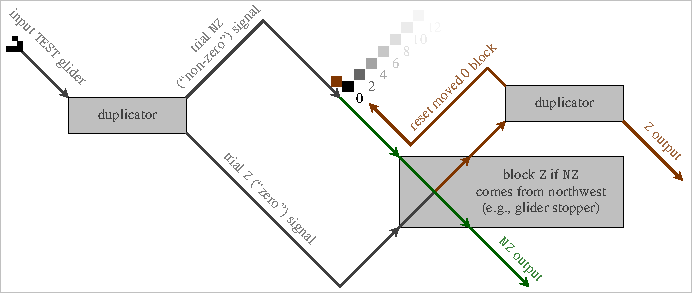
\includegraphics[width=\textwidth]{universal_computation/sliding_block_schematic.pdf}
	\caption{A schematic of a \texttt{TEST} circuit that tests whether or not a sliding block is in the ``zero'' (\texttt{Z}) position. If the block is in a non-zero (\texttt{NZ}) position then the trial \texttt{NZ} glider passes by without affecting it at all. Otherwise, the zero block is shifted via the $(2,1)$ block pull reaction, the trial \texttt{NZ} glider is destroyed, and the \texttt{Z} glider performs another $(2,1)$ block pull to put that zero block back in its original place.}\label{fig:sliding_block_schematic}
\end{figure}

We could then create a complete sliding block register by adding two additional inputs beyond just the \texttt{TEST} input:\smallskip

\begin{itemize}
	\item a \texttt{DEC} input that produces two gliders that are aimed at the sliding block as in Figure~\ref{fig:synchronized_block_mover_4}, so as to pull the block one cell closer, and\smallskip
	
	\item an \texttt{INC} input that produces the three gliders from Figure~\ref{fig:synchronized_block_mover_5} (two of which are the same as the gliders produced for the \texttt{DEC} operation), so as to push the block one cell farther away.\smallskip
\end{itemize}

A sliding block register with these three inputs could certainly be used in a Life computer, but we would have to be very careful never to write a program that might accidentally send a \texttt{DEC} signal when the block is already at the ``zero'' position. After all, if that ever happened then the \texttt{TEST} mechanism would fail catastrophically, because the glider that's supposed to graze the block so as to perform the (2,1) block pull reaction would instead run right into it.\footnote{By contrast, \texttt{INC} operations will never cause problems---it's always possible to move the block out by one more step to store the integer $n+1$ instead of $n$, so only \texttt{DEC} instructions are potentially dangerous.}

Our program could avoid this danger by always calling \texttt{TEST} first, and then only calling \texttt{DEC} if an \texttt{NZ} output comes back from \texttt{TEST}. However, a better option is to instead bake this idea right into the sliding block register itself, rather than relying on the programs that we write to do so. That is, we adjust the design of the sliding block register so that a \texttt{TEST} always happens just before a \texttt{DEC}. The circuit itself will then ignore the \texttt{DEC} input if the block is already at the \texttt{Z} position.

This slight redesign gives us an equally useful (and much safer!) sliding block register that has only two inputs: \texttt{INC} and \texttt{TEST}-then-\texttt{DEC}, which we abbreviate as \texttt{TDEC}.\index{TDEC} In this register, which is illustrated in Figure~\ref{fig:sliding_block_register}, there is no longer a way to send in a series of inputs that causes a catastrophic failure. Note that we have made the output \texttt{Z} and \texttt{NZ} lanes of this particular sliding block register transparent\index{transparent!lane} so that multiple registers can easily be placed side-by-side.

\begin{figure}[!htb]
	\centering
	\embedlink{sliding_block_register}{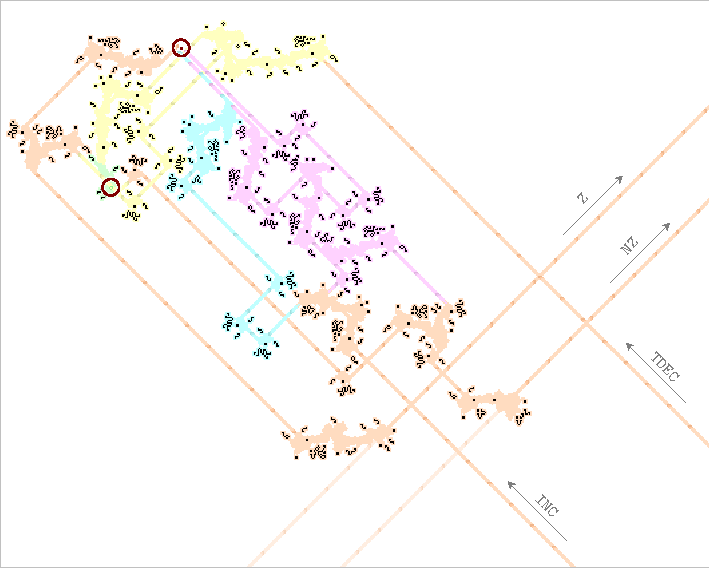
\includegraphics[width=\textwidth]{universal_computation/sliding_block_register.pdf}}
	\caption{A sliding block register. If a glider enters on the \texttt{INC} lane, the \bgbox{aquaback}{aqua} and \bgbox{magentaback}{magenta} conduits split it into three gliders that push the sliding block (circled in \bgbox{redback}{red} near the top) northwest by $1$ cell. If a glider enters on the \texttt{TDEC} lane, it enters the \texttt{TEST} circuit (the first half of which is highlighted in \bgbox{yellowback2}{yellow}). That \texttt{TEST} circuit uses a demultiplexer (highlighted in \bgbox{greenpastel}{green}) to switch the path of the glider---if the block is in the ``zero'' position then the glider passes through the demultiplexer to the northwest on the \texttt{Z} output path, and otherwise the demultiplexer creates a boat (circled in \bgbox{redback}{red} near the top-left) that redirects the glider to the northeast on the \texttt{NZ} output path. In the latter case, the \texttt{NZ} output glider is also fed into the \bgbox{magentaback}{magenta} conduit that creates two gliders to pull the sliding block $1$ cell southeast.}\label{fig:sliding_block_register}
\end{figure}


%%%%%%%%%%%%%%%%%%%%%%%%%%%%%%%%%%%%%%%%%%%%%%%%%%%%%%%%%%%%%%%%%%%%%%%%%
%%   SUBSECTION: ASSEMBLY CODE FOR A FINITE-STATE MACHINE
%%%%%%%%%%%%%%%%%%%%%%%%%%%%%%%%%%%%%%%%%%%%%%%%%%%%%%%%%%%%%%%%%%%%%%%%%
\subsection{Assembly Code for a Finite-State Machine}\label{sec:finite_state_machine}

We now have a mechanism that can store integer values, with two simple inputs (\texttt{INC} and \texttt{TDEC}) and two simple outputs (\texttt{Z} and \texttt{NZ}). Before delving into the details of how to position these registers on the Life plane to carry out computations, we first spend some time thinking about how to perform computations that only involve the operations corresponding to their input lanes---increasing or decreasing the value of some register, and checking whether or not a register is currently equal to zero.

To give a rough idea of how we could carry out a computation of this type, consider the task of just checking which of two registers contains a smaller value. We can solve this problem by repeatedly decrementing the value of the registers, and stopping once either of them is storing a value of \texttt{0}. Whichever one hits \texttt{0} first is determined to be the register that started off storing the smaller value. Pseudocode that implements this algorithm is provided by Pseudocode~\ref{alg:pseudocode_test_leq_or_ge}.

When we write pseudocode like this, we use labels like \texttt{U0}, \texttt{U1}, \texttt{U2}, $\ldots$ to denote the various registers used by the computer program.\footnote{The ``\texttt{U}'' stands for the word \textbf{unary}, since these sliding block registers stores integers in unary (i.e., the base-$1$ numeral system). We will see a different type of register that instead stores integers in binary a bit later, in Section~\ref{sec:binary_register}.} Also, for this particular pseudocode it is intended that the computer starts by executing the first line of code, then automatically moves to the following line and executes that, and so on---unless it encounters an instruction that tells it to \texttt{HALT} or jump to some other line of the program.

\begin{pseudocode}[!htb]
	\begin{algorithmic}[1]\small
		\State \texttt{if U0 = 0, jump to 6}
		\State \texttt{if U1 = 0, jump to 8}
		\State \texttt{decrement U0}
		\State \texttt{decrement U1}
		\State \texttt{jump to 1}
		\State \texttt{OUTPUT "U0 <= U1"}
		\State \texttt{HALT}
		\State \texttt{OUTPUT "U1 < U0"}
		\State \texttt{HALT}
	\end{algorithmic}
	\caption{Test which of the registers \texttt{U0} or \texttt{U1} contains a smaller value.}\label{alg:pseudocode_test_leq_or_ge}
\end{pseudocode}

Our next goal is to simplify and standardize our pseudocode so as to make it simpler to implement as a Life pattern. With this in mind, a \textbf{finite-state machine}\index{finite-state machine} is a model of computation in which the computer can be in one of a finite number of states at any given time, and its state can change based on inputs that it receives. We can implement a finite-state machine with $n$ possible states via a Life pattern that has a single glider traversing a set of $n$ parallel lanes connected by other circuitry.  At any given computer clock tick, the glider will be on exactly one of the ``state'' lanes. It will then run through structures that send gliders to various inputs of various register circuits, and also send a glider to the lane representing the next state in the program.

In order for our pseudocode to more accurately reflect this finite-state machine that our Life program will implement, we require $2$ additional things of all pseudocode that we write from this point forward:\smallskip

\begin{itemize}
	\item[1)] We include a ``jump'' instruction at the end of every single line. This corresponds to specifying exactly what state transition happens at each computer clock tick in the finite-state machine that we are implementing.\footnote{Our pseudocode, and the programming language that we will develop based on it, is thus one of the few examples of a language where execution does \emph{not} automatically proceed from one line to the next. For a more ``real-world'' example of such a language, see for example RPC-4000 machine code, as described in The Story of Mel: \httpurl{catb.org/jargon/html/story-of-mel.html}}\smallskip
	
	\item[2)] All conditional statements that we include are conditioned on whether the last output value received from a register was \texttt{Z} or \texttt{NZ}. We thus have to be careful to make sure that we always perform some task (like a \texttt{TDEC}) that returns a \texttt{Z} or \texttt{NZ} value immediately before jumping to a conditional statement.\smallskip
\end{itemize}

By making the changes outlined in points (1) and (2) above, our original Pseudocode~\ref{alg:pseudocode_test_leq_or_ge} is transformed into Pseudocode~\ref{alg:fsm_test_leq_or_ge}. These pseudocodes implement the same computational task (determining which of the two registers \texttt{U0} and \texttt{U1} is storing a smaller value), but the new pseudocode will be simpler for us to implement as a Life pattern. In particular, each line in Pseudocode~\ref{alg:fsm_test_leq_or_ge} now corresponds to a state in the finite-state machine that we will implement. This machine will start in the state of Line 1, and will move from state to state (i.e., line to line) until the algorithm has completed its work. Eventually either one output or the other will be sent out, and the program will reach its \texttt{HALT} state.

\begin{pseudocode}
	\begin{algorithmic}[1]\small
		\State \texttt{TDEC U0; jump to 2}
		\State \texttt{if return=Z then jump to 5, otherwise jump to 3}
		\State \texttt{TDEC U1; jump to 4}
		\State \texttt{if return=Z then jump to 6, otherwise jump to 1}
		\State \texttt{OUTPUT "U0 <= U1"; jump to 7}
		\State \texttt{OUTPUT "U1 < U0"; jump to 7}
		\State \texttt{HALT}
	\end{algorithmic}
	\caption{Test which of the registers \texttt{U0} or \texttt{U1} contains a smaller value---second version.}\label{alg:fsm_test_leq_or_ge}
\end{pseudocode}

We now refine this pseudocode even further and standardize it into what we call\index{APGsembly} \textbf{APGsembly code}---the programming language that we will use to write and compile computer programs in Life patterns.\footnote{The name ``APGsembly'' is a play on the word ``assembly'' (low-level code for programming computer instructions) and the initials of its author, Adam~P. Goucher. Indeed, APGsembly was used by Goucher to construct the original $\pi$ calculator in 2010.} In order to make the conditional statements of our pseudocode even easier to implement, we split each state of the finite state machine (i.e., our ``computer'') into two substates: one corresponding to the most recent return value being \texttt{Z}, and one corresponding to the most recent return value being \texttt{NZ}. These substates may result in completely different actions being taken and may cause the program to subsequently jump to completely different states (just as in a regular conditional statement).\footnote{In the actual Life implementation of the finite-state machine, this will mean that a glider will appear on one of two different parallel lanes during any given state, depending on whether the last output value received from a register was \texttt{Z} or \texttt{NZ}.}

Once we make the above change, we no longer really need logical instructions in our pseudocode at all: every program can be specified by listing what actions should be taken (e.g., \texttt{INC} or \texttt{TDEC}) when a particular state and substate is encountered, along with which state should then be jumped to next. See APGsembly~\ref{alg:apgsembly_test_leq_or_ge} for our first concrete example of APGsembly code---it implements the same ``does \texttt{U0} contain a smaller value than \texttt{U1}?'' test that we saw in Pseudocode~\ref{alg:fsm_test_leq_or_ge}.

\begin{apgsembly}
	\begin{algorithmic}\small
		\State \verb|# State    Input    Next state    Actions|
		\State \verb|# ---------------------------------------|
		\State \verb|INITIAL;   ZZ;      ID1;          TDEC U0|
		\State \verb|ID1;       Z;       ID2;          OUTPUT 0, HALT_OUT|
		\State \verb|ID1;       NZ;      ID2;          TDEC U1|
		\State \verb|ID2;       Z;       ID1;          OUTPUT 1, HALT_OUT|
		\State \verb|ID2;       NZ;      ID1;          TDEC U0|
	\end{algorithmic}
	\caption{APGsembly code to test which of the registers \texttt{U0} or \texttt{U1} contains a smaller value. An output value of \texttt{0} indicates that \texttt{U0 <= U1}, while an output value of \texttt{1} indicates that \texttt{U1 < U0}.}\label{alg:apgsembly_test_leq_or_ge}
\end{apgsembly}

On its surface, this APGsembly code looks quite different from the pseudocode that we saw earlier, so it is a good idea to trace through the program flow carefully until you are comfortable with the fact that it really does implement the exact same algorithm that we already saw. We now describe how APGsembly code is written, and how it differs from the pseudocode that we saw earlier:\smallskip

\begin{itemize}
	\item Line numbers from our pseudocode have been replaced by paired \texttt{ID} labels. Each state can have any alphanumeric ID label of our choosing, with the exception of the first, which is always called \texttt{INITIAL}.\footnote{Also, the \texttt{INITIAL} state should never be returned to later in a program's execution. It should be the first state, and \emph{only} the first state.} Using IDs like this instead of line numbers makes it much easier to manage our code---if we were to continue using line numbers instead of labels then we would have to update every single one of our ``jump'' instructions if we ever inserted a new line of code.\smallskip
	
	\item There are no longer any explicit ``if'' statements in the code, since each state (pair of lines sharing an ID label) acts implicitly as an ``if'' statement. \emph{If} the return value (from the previous action) is \texttt{Z}, perform the actions given on the first (\texttt{Z}) line; \emph{otherwise} perform the actions given in the second (\texttt{NZ}) line.\smallskip
	
	\item Sometimes, a particular state can only ever be reached by a \texttt{Z} input, so it does not need a corresponding \texttt{NZ} substate. In this case, the \texttt{NZ} substate can be omitted from the APGsembly code, and the \texttt{Z} substate is instead denoted by \texttt{ZZ} so that the compiler knows that the \texttt{NZ} omission was intentional. The \texttt{INITIAL} state is always assumed to have a \texttt{Z} input (just because the computer has to start in \emph{some} substate) and thus the first line of APGsembly code always starts with \texttt{INITIAL;ZZ}.\footnote{Similarly, if a state performs the exact same actions and jump operation regardless of whether it receives a \texttt{Z} or \texttt{NZ} return value, we can just list a single line for that state with \texttt{*} as its input value, instead of two otherwise identical lines with \texttt{Z} and \texttt{NZ} as their input values. We will not see an example of this in the main text, but it appears in Appendix~\ref{sec:appendix_apg}.}\smallskip
	
	\item Each line contains four items, separated by semicolons: state ID, input value, next state ID, and a comma-separated list of actions. The ``next state'' ID tells the program which state ID to jump to after performing the actions listed on the current line.\smallskip
	
	\item To make code easier to read, we can add comments to our code via lines that start with \texttt{\#} (so the first two lines of APGsembly~\ref{alg:apgsembly_test_leq_or_ge} do not actually affect what the code does, but just help us keep track of the four items on each line of code). For a similar reason, we can include any white space of our choosing between pieces of code, and empty lines between states if desired.\smallskip
	
	\item The \texttt{OUTPUT 0} and \texttt{OUTPUT 1} actions tell the Life computer to print out either a \texttt{0} or a \texttt{1} on the Life plane, in a font made up of blocks. We will see how this printing is actually done in Section~\ref{sec:decimal_printer}, but for now we note that by default this action can only print the digits \texttt{0}--\texttt{9} and periods (\texttt{.}), not more complicated expressions like ``\texttt{U0<=U1}''.\footnote{However, we will see in Section\ref{sec:decimal_printer} that this printing can, with slightly more work, be extended to any set of characters of our choosing.} The \texttt{HALT\_OUT} action stops the computer\footnote{For this reason, the ``next state'' provided in lines containing a \texttt{HALT\_OUT} action does not actually matter, since the computer never actually proceeds past that point.} (presumably because we are done our desired computation) and emits an output glider that could then be used by another pattern on the Life plane to detect that the computation finished.\smallskip
\end{itemize}

There are a few restrictions on what combinations of actions can be performed in a single line of APGsembly code. One of the reasons for this is that all actions on a particular line of APGsembly code are performed simultaneously, rather than sequentially. We should thus avoid single-line lists of actions like ``\texttt{TDEC U0, INC U0}'', for example, since the result of the \texttt{TDEC} may depend on whether or not the \texttt{INC} has already been completed, which is unpredictable. If the order of actions matters, they should be split into states on multiple different lines.

Furthermore, because of how these actions will be implemented in our Life computer (which we explore in the upcoming Section~\ref{sec:compiled_add_two_registers}), it is not possible to perform the same action more than once in a single substate (i.e., line of APGsembly). For example, if we want to increase the value of the register \texttt{U0} by \texttt{2}, it is tempting to use the list of actions ``\texttt{INC U0, INC U0}'' in a single line of APGsembly. However, this must be avoided---we should instead perform the first \texttt{INC U0}, then jump to another state, and then perform the next \texttt{INC U0}.

One final restriction comes from the fact that the return value from one line of APGsembly code dictates which substate of the next state is executed, so each line of APGsembly must contain exactly one action that produces a return value. If multiple actions were to produce a return value then it would not be clear which substate should be jumped to next, and if no action produced a return value then no substate would be jumped to and the computer would stop running altogether.\footnote{As a technical note, the \texttt{HALT\_OUT} action does not actually produce a return value (it does not need to, since we \emph{want} the computer to stop when it encounters \texttt{HALT\_OUT}). Instead, it is just a special action that bypasses the need for every line to have a return value.} So far, \texttt{TDEC} is the only action that we have introduced that produces a return value. Future sections will introduce some additional logic components that include value-returning actions, and a summary of these components and actions can be found by jumping ahead to Table~\ref{tab:universal_computation_components}. But first, let's take a look at what a compiled Life pattern arising from APGsembly code actually looks like.


%%%%%%%%%%%%%%%%%%%%%%%%%%%%%%%%%%%%%%%%%%%%%%%%%%%%%%%%%%%%%%%%%%%%%%%%%
%%   SECTION: A COMPILED APGSEMBLY PATTERN
%%%%%%%%%%%%%%%%%%%%%%%%%%%%%%%%%%%%%%%%%%%%%%%%%%%%%%%%%%%%%%%%%%%%%%%%%
\section{A Compiled APGsembly Pattern: Adding Registers}\label{sec:compiled_add_two_registers}

APGsembly code is specifically designed so that it can straightforwardly be compiled into a Life pattern.\footnote{Links to an APGsembly compiler, and some emulators that can be used to help debug APGsembly programs, can be found at \httpsurl{conwaylife.com/wiki/APGsembly}.} We now illustrate how this is done by constructing a Life computer that adds the values of two sliding block registers.

Our first step toward building such a computer is to write APGsembly code that implements the desired computational task. The code in APGsembly~\ref{alg:apgsembly_add_same_register} does the job nicely---it works by repeatedly decreasing the value of one register until it reaches a value of \texttt{0}, while simultaneously increasing the value of the other register every time. The only pieces of this APGsembly that we have not yet seen are the ``\texttt{\#COMPONENTS}'' and ``\texttt{\#REGISTERS}'' lines in the APGsembly's header. These lines are used to tell the APGsembly compiler which registers are used in the code,\footnote{``\texttt{U0-1}'' means that the code uses registers \texttt{U0} and \texttt{U1}. The ``\texttt{-}'' indicates a range (so ``\texttt{U0-2}'' would refer to registers \texttt{U0}, \texttt{U1}, and \texttt{U2}, for example).} and what the initial values of the registers should be, respectively. If a register is not initialized via the \texttt{\#REGISTERS} line, it starts with a value of \texttt{0}.

\begin{apgsembly}
	\begin{algorithmic}\small
		\State \verb|#COMPONENTS U0-1,HALT_OUT|
		\State \verb|#REGISTERS {'U0':7, 'U1':5}|
		\State \verb|# State    Input    Next state    Actions|
		\State \verb|# ---------------------------------------|
		\State \verb|INITIAL;   ZZ;      ID1;          TDEC U0|
		\State \verb|ID1;       Z;       ID1;          HALT_OUT|
		\State \verb|ID1;       NZ;      ID1;          TDEC U0, INC U1|
	\end{algorithmic}
	\caption{APGsembly code to add the value of \texttt{U0} to \texttt{U1}, and zero out \texttt{U0}. The \texttt{\#REGISTERS} line pre-loads the registers with the values \texttt{7} and \texttt{5}, respectively (so that after the computation completes, we will have \texttt{U0 = 0} and \texttt{U1 = 12}).}\label{alg:apgsembly_add_same_register}
\end{apgsembly}

While this code is quite simple (it's only $3$ lines long!), it illustrates an important oddity of APGsembly that we must keep in mind. Since \texttt{TDEC} is short for ``test and \emph{then} decrement'', it has the somewhat counterintuitive feature of giving a \texttt{Z} or \texttt{NZ} return value that is based on the value that was contained in it \emph{before} it was decremented. In particular, if we use a \texttt{TDEC} to decrement a register from 1 to 0, the return value will be \texttt{NZ}, not \texttt{Z}!

For this reason, APGsembly loops based on the \texttt{TDEC} action often require one more iteration than might be expected at first. If we want to decrement the value of a register from $n$ down to $0$, we have to call \texttt{TDEC} $n$ times. However, we then have to call it $1$ more time (which does not actually affect the value of the register, since it cannot decrease below $0$) in order to get a return value of \texttt{Z} instead of \texttt{NZ} and break out of the loop.

Since APGsembly code requires an action in the \texttt{INITIAL} state anyway before any loops are entered, we often put the extra \texttt{TDEC} command there (we did this in each of APGsembly~\ref{alg:apgsembly_test_leq_or_ge} and~\ref{alg:apgsembly_add_same_register}). The resulting code has the effect of decreasing the value of the register from $n$ to $n-1$, then looping from $n-1$ to $-1$, but with the register getting stuck at $0$ instead of actually decrementing all the way down to $-1$.

An actual Life pattern that implements the computation described by APGsembly~\ref{alg:apgsembly_add_same_register} is presented in Figure~\ref{fig:add_computer}. There is a lot going on in this pattern, so we now describe how it is built in some detail. This computer (and Life computers built from APGsembly in general) consists of three main parts: a \textbf{computer}\index{computer} (in the southeast), a \textbf{component stack}\index{component stack} (in the northwest), and a \textbf{clock gun} (in the north). We describe these three pieces one at a time.\index{component stack}\index{computer}\index{clock!gun}

\begin{figure}[!htb]
	\centering
	\embedlink{add_computer}{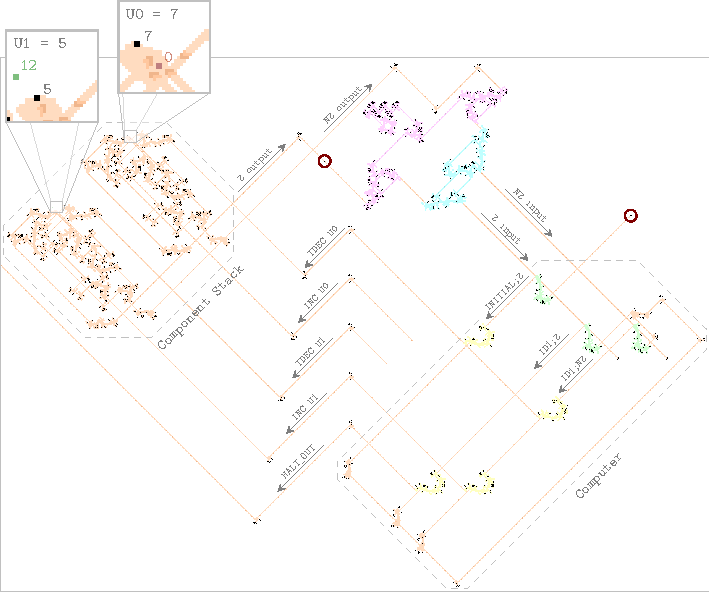
\includegraphics[width=\textwidth]{universal_computation/add_computer.pdf}}
	\caption{A compiled Life pattern that adds the values of the registers \texttt{U0} and \texttt{U1} (which have been pre-loaded with the values \texttt{7} and \texttt{5}, respectively), as in APGsembly~\ref{alg:apgsembly_add_same_register}. The registers at the west feed their output into the period~$2^{20}$ clock gun (highlighted in \bgbox{magentaback}{magenta} with two separate universal regulators---one for the \texttt{Z} path and another for the \texttt{NZ} path). The clock gun feeds a glider into a demultiplexer (highlighted in \bgbox{greenpastel}{green}) corresponding to the next substate of the computer (i.e., line of APGsembly). That demultiplexer then feeds into splitters (highlighted in \bgbox{yellowback2}{yellow}) corresponding to the actions in that line of APGsembly (the \texttt{INC U0} and \texttt{TDEC U1} lanes are disconnected from the computer because those actions are not called by any line of APGsembly~\ref{alg:apgsembly_add_same_register}). Finally, the duplicated gliders heading to the northwest feed back into the registers, and the duplicated glider heading to the southwest is reflected around the southeast end of the computer so as to activate the demultiplexer for its next state. The conduit highlighted in \bgbox{aquaback}{aqua} puts the \texttt{Z} or \texttt{NZ} glider coming from the clock gun on the correct input lane, and then produces an extra cleanup glider on each computer input lane so as to reset the demultiplexers. The two gliders circled in \bgbox{redback}{red} start the computation by activating the \texttt{INITIAL;Z} demultiplexer and then feeding a glider into it.}\label{fig:add_computer}
\end{figure}


\subsection{The Computer}

The computer is an implementation of a finite-state machine, so when it is at rest it is always in one of a finite number of different states, represented by a pair of demultiplexers that have a boat. Either a \texttt{Z} or an \texttt{NZ} signal will head southeast from the clock gun as a result of the computation performed in the computer's previous state. That glider will hit either the \texttt{Z} or the \texttt{NZ} demultiplexer and be reflected toward the southwest on a lane corresponding to exactly one specific line of APGsembly code.

If the computer is currently in state \texttt{ID1}, for example, then the two demultiplexers representing the \texttt{ID1} state both contain boats. If a \texttt{Z} signal comes in, the \texttt{Z} boat turns a glider onto the \texttt{ID1;Z} lane, and the \texttt{NZ} boat is cleaned up by a following glider. Conversely, if an \texttt{NZ} signal comes in, the \texttt{NZ} boat turns a glider onto the \texttt{ID1;NZ} lane, and the \texttt{Z} boat gets cleaned up instead.

The glider heading southwest then passes through one or more splitters---glider duplicators\index{splitter} that create a perpendicular glider while also sending another glider to continue along the exact same lane. As many splitters as we desire can thus be added along these lanes without changing the final destination of the southwest-travelling glider. Each splitter sends a glider on an output lane corresponding to an action from the current line of APGsembly code: \texttt{TDEC U0}, \texttt{INC U1}, and so on.

After going through the sequence of splitters, the southwest-bound glider hits a merge circuit---a reflector that is transparent to signals passing through it on its output lane. This implements the ``jump to'' part of each APGsembly line, and the transparency allows multiple lines of APGsembly to jump to the same state. Indeed, multiple merge circuits on the same northwest-to-southeast diagonal all produce gliders on the same lane, which are routed around to trigger the pair of demultiplexers for the next target state.\footnote{The computer in Figure~\ref{fig:add_computer} only has one path around its southern corner along which gliders can be reflected back into the demultiplexers. This is because every single line of APGsembly~\ref{alg:apgsembly_add_same_register} that generated that computer tells it to jump to the same state (\texttt{ID1}). We will see other computers shortly that can jump to multiple different states and thus have more glider paths down there.} The two boats then wait in the demultiplexer for the next \texttt{Z} or \texttt{NZ} signal from the clock.

As a technical implementation note, recall that the \texttt{INITIAL} state is always assumed to have a \texttt{Z} input. That \texttt{Z} input is hard-coded into the Life pattern in order to start the computation. The computer displayed in Figure~\ref{fig:add_computer} does not even have an \texttt{INITIAL;NZ} substate, since it would be impossible to reach anyway---recall that this is why the \texttt{INITIAL;Z} substate was listed as \texttt{INITIAL;ZZ} in APGsembly~\ref{alg:apgsembly_add_same_register}.


\subsection{The Component Stack}

In these calculator patterns, information is stored separately from the computer, in an array of ``components''. These components each have a finite number of inputs (called ``actions'' in APGsembly code) that can be used to manipulate or retrieve that information, and they potentially provide a single \texttt{Z}/\texttt{NZ} output bit. The first example that we have seen is the sliding block register, which has two action inputs (\texttt{INC Un} and \texttt{TDEC Un}) and the two standard outputs (\texttt{Z} and \texttt{NZ}). Since their output lanes are transparent, any number of sliding block registers \texttt{U0}, \texttt{U1}, \texttt{U2},$\ldots$ can be stacked side-by-side, and APGsembly code can \texttt{INC} or \texttt{TDEC} any one of them. If there are a lot of registers, the computer part of the pattern has to be stretched a little wider to accommodate spaces for more splitters. The computer has to be wide enough to hold two splitters for each sliding-block register---one for each \texttt{INC} action and one for each \texttt{TDEC} action.

Other components may have more or fewer action inputs. For example, we will see a binary register in Section~\ref{sec:binary_register} that has four actions: \texttt{INC Bn}, \texttt{TDEC Bn}, \texttt{READ Bn}, and \texttt{SET Bn}. New components could be designed to perform any logical function or store any amount of information that we might want; we will see an example of this in Section~\ref{sec:Osqrtlogt}, with the two-dimensional memory storage ``\texttt{B2D}'' component.

No matter how many components are added to the stack, they're all called in the same way, by a single glider travelling northwest on an ``action'' lane. Multiple actions can be triggered simultaneously, though each component may be activated at slightly different times depending on where it is placed in the stack. Since the precise timing of the actions depends heavily on how the computer and component stack are wired together, it is strongly recommended that a single line of code in APGsembly never triggers more than one action in a particular component. While it does not always cause problems, calling two simultaneous actions would cause many of the components that we consider here to fail. This problem can be avoided simply by calling the two incompatible actions from separate states (i.e., lines of APGsembly code).


\subsection{The Clock Gun}

Once a \texttt{Z} or \texttt{NZ} output signal is generated by the component stack, it is fed back into the computer in order to jump to the next state. However, we have to be slightly careful about when this glider arrives at the computer---we have to be sure that it does not arrive before the next state's demultiplexers are set in the computer (i.e., before the computer's glider has had a chance to go through the merge circuits and find its way all the way around the southern perimeter of the computer part of the pattern).\footnote{This is not much of a concern in the pattern from Figure~\ref{fig:add_computer} since the path around the computer is so short, but it becomes an issue for patterns with larger computers (i.e., patterns generated by more lines of APGsembly).}

To delay the component stack's output glider, we could simply extend the length of the path that it must follow back to the computer. However, we instead make use of a very high-period universal regulator.\index{universal regulator} The advantage of this method is that several pieces of the pattern then repeat predictably at the period of the universal regulator, which lets Life simulation software evolve it much quicker than it could if the glider timing was less regular. In particular, if we choose the universal regulator to align to some high power-of-two period, then Golly's \emph{HashLife}\index{HashLife} algorithm is able to evolve these patterns extremely quickly.\footnote{HashLife is an algorithm for simulating Life that was developed by Bill Gosper in 1984 \cite{Gos84}. It works by creating a lookup table that keeps track of how the $2^{n} \times 2^{n}$ center of certain repetitive $2^{n+1} \times 2^{n+1}$ chunks of a pattern evolve over $2^{n-1}$ generations. Since nothing outside of that $2^{n+1} \times 2^{n+1}$ square can affect its $2^{n} \times 2^{n}$ center within those $2^{n-1}$ generations, the results of that computation can simply be re-used whenever that same square is encountered in the future.}

The universal regulator that we use\footnote{Constructed by ConwayLife.com forums user ``Jormungant'' in April 2020.} is conceptually very simple. A stream of gliders coming from a gun of any (sufficiently large) period of our choosing comes in from the northeast and is split into two streams that destroy each other. However, if a glider comes in from the northwest then it is fed into a syringe and then one of the Herschel-to-boat factories from Figure~\ref{fig:H_to_boat}. The resulting boat suppresses a single glider from the gun's duplicated stream, letting a glider that is aligned to the period of that gun escape, as illustrated in Figure~\ref{fig:stable_universal_regulator}.

The gun that we attach to this universal regulator has period $2^{20}$, which we choose simply because it is a power of $2$ that is large enough to handle most of the calculators that we will construct in this chapter, but small enough that it can be simulated quickly in software like Golly. To actually construct this gun, we just do exactly what we did in Section~\ref{sec:large_glider_guns}: we attach period multipliers to another gun. This particular gun (displayed in Figure~\ref{fig:p2to_the_20_gun}) uses quadri-Snarks (see Exercise~\ref{exer:quadri_snark}) \index{quadri-Snark} attached to a p$256$ machine gun,\index{machine gun} but semi-Snarks could have been used instead at the expense of the gun being slightly larger.

\begin{figure}[!htb]
	\centering
	\begin{minipage}[t]{0.47\textwidth}
		\centering
		\embedlink{stable_universal_regulator}{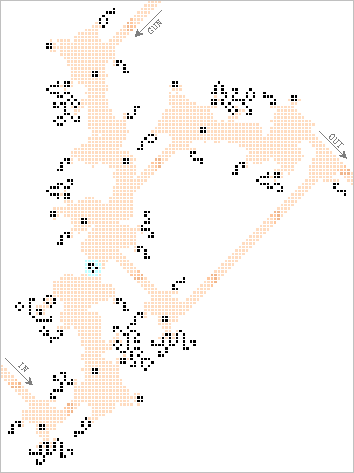
\includegraphics[width=0.9\textwidth]{universal_computation/stable_universal_regulator.pdf}}
		\caption{A stable universal regulator that works by having the input glider create a boat (highlighted in \bgbox{aquaback}{aqua}), which suppresses the glider on the southeast path and allows the northeast glider to escape.}\label{fig:stable_universal_regulator}
	\end{minipage}\hfill
	\begin{minipage}[t]{0.49\textwidth}
		\centering
		\patternimglink{0.135}{p2to_the_20_gun}
		\caption{A period~$2^{20}$ gun that works by using $6$ quadri-Snarks (highlighted in \bgbox{aquaback}{aqua} and \bgbox{magentaback}{magenta}) to repeatedly quadruple the period of a p$256$ machine gun.}\label{fig:p2to_the_20_gun}
	\end{minipage}
\end{figure}

The high-period universal regulator that results from stitching together Figures~\ref{fig:stable_universal_regulator} and~\ref{fig:p2to_the_20_gun} is called the \textbf{clock gun}, and it determines the speed at which the pattern computes whatever it has been programmed to compute. We think of the period of this clock gun as the clock speed of the computer, and one period of the regulator as one clock tick or computational cycle.\footnote{Some computations may take longer than one clock tick to complete, but that's okay. For example, if a sliding block register is storing an extremely large value then its sliding block will be extremely far away from the computer, so it will take a long time to \texttt{INC} or \texttt{TDEC}. In this case, the clock gun simply waits for one or more clock ticks until an output signal is received from the component stack.}

In summary, the calculator patterns that we compile from APGsembly work as follows:\smallskip

\begin{itemize}
	\item The computer in the southeast corner keeps track of the state and sends action commands to the component stack.\smallskip
	
	\item The action commands alter the contents of the components in the component stack, which serve as the computer's memory. Exactly one of these components then sends an output signal (glider) to the clock gun.\smallskip
	
	\item The clock gun regulates the glider signal coming from the component stack and feeds it back into the computer.
\end{itemize}


%%%%%%%%%%%%%%%%%%%%%%%%%%%%%%%%%%%%%%%%%%%%%%%%%%%%%%%%%%%%%%%%%%%%%%%%%
%%   SECTION: MULTIPLY TWO REGISTERS
%%%%%%%%%%%%%%%%%%%%%%%%%%%%%%%%%%%%%%%%%%%%%%%%%%%%%%%%%%%%%%%%%%%%%%%%%
\section{Multiplying and Re-Using Registers}\label{sec:multiply_two_registers}

Now that we understand how to \emph{add} the value of two sliding block registers, we ramp up to the problem of \emph{multiplying} their values. One seemingly simple method of multiplying \texttt{U0} by \texttt{U1} and storing the result in \texttt{U2} would be to repeatedly add the register \texttt{U1} to \texttt{U2} a total of \texttt{U0} times. However, there is a slightly problem with this idea---our method of adding two registers from APGsembly~\ref{alg:apgsembly_add_same_register} zeroes out one of the registers while adding it to the other. Indeed, the only method that we have of looping over one register is based on \texttt{TDEC}ing it until it hits \texttt{0}, thus erasing the value that register contained.

To get around this problem, we introduce a temporary register into which we copy the value of one of the registers that we wish to loop over, and then we loop over that temporary register instead. In this particular case of setting \texttt{U2 = U0 * U1}, every time we add \texttt{U1} to \texttt{U2}, we do so by first copying \texttt{U1} to a new temporary register \texttt{U3} (zeroing out \texttt{U1} in the process), and then looping over \texttt{U3} so as to add it to each of \texttt{U1} \emph{and} \texttt{U2}. Pseudocode for carrying out this task, as well as the corresponding APGsembly code, is presented in APGsembly~\ref{apg:mult_unary_reg}.\footnote{After this code is executed, the value of \texttt{U1} is preserved, but the value of \texttt{U0} is not. If we want to preserve the value of \texttt{U0}, we can use \emph{another} temporary register (see Exercise~\ref{exer:universal_computation_mult_preserve_r0}).}

\begin{apgsembly}
	\centering
	\begin{minipage}[t]{.49\textwidth}
		\begin{algorithmic}[1]\small
			\State\texttt{TDEC U0}
			\State\texttt{if return value = Z:}
			\State\texttt{~~~~\# Loop U0 times, then halt.}
			\State\texttt{~~~~HALT}
			\State\texttt{else:}
			\State\texttt{~~~~\# Add U1 to U2 without erasing U1}
			\State\texttt{~~~~set U3 = U1}
			\State\texttt{~~~~set U1 = U3, U2 = U2 + U3}
			\State\texttt{end if}
			\State\texttt{jump to 1}
		\end{algorithmic}
	\end{minipage}\hfill{\color{gray}\vline}\hfill
	\begin{minipage}[t]{.49\textwidth}
		\begin{algorithmic}\tiny
			\State \verb|#COMPONENTS U0-3,HALT_OUT|
			\State \verb|#REGISTERS {'U0':7, 'U1':5}|
			\State \verb|# State    Input    Next state    Actions|
			\State \verb|# ---------------------------------------|
			\State \verb|INITIAL;   ZZ;      ID1;          TDEC U0|
			\State \verb||
			\State \verb|# Loop over U0, TDECing it until it hits 0, and then halt.|
			\State \verb|ID1;       Z;       ID1;          HALT_OUT|
			\State \verb|ID1;       NZ;      ID2;          TDEC U1|
			\State \verb||
			\State \verb|# Copy U1 into U3 while setting U1 = 0.|
			\State \verb|ID2;       Z;       ID3;          TDEC U3|
			\State \verb|ID2;       NZ;      ID2;          TDEC U1, INC U3|
			\State \verb||
			\State \verb|# Loop over U3, adding its value to U1 (restoring it) and U2.|
			\State \verb|ID3;       Z;       ID1;          TDEC U0|
			\State \verb|ID3;       NZ;      ID3;          TDEC U3, INC U1, INC U2|
		\end{algorithmic}
	\end{minipage}
	\caption{Pseudocode (left) and APGsembly code (right) to set \texttt{U2 = U0 * U1} and zero out \texttt{U0}. The register \texttt{U3} is used just temporarily (it starts and ends at the value of \texttt{0}) to store the value of \texttt{U1}. After this computation completes, the registers will have the values \texttt{U0 = 0}, \texttt{U1 = 5}, \texttt{U2 = 35}, and \texttt{U3 = 0}.}\label{apg:mult_unary_reg}
\end{apgsembly}

A Life pattern that was compiled from APGsembly~\ref{apg:mult_unary_reg} is displayed in Figure~\ref{fig:mult_computer}. This multiplication pattern has the same general shape and structure as the addition pattern from Figure~\ref{fig:add_computer}, but with slightly more of everything---$4$ sliding block registers instead of $2$, $7$ subtates in the computer (corresponding to the $7$ lines of APGsembly code) instead of $3$, and so on. Perhaps the most notable change in this calculator pattern is that there are now $3$ glider lanes looping around the southern perimeter of the computer, whereas there was only $1$ such lane in Figure~\ref{fig:add_computer}. These extra lanes correspond to the fact that there are lines of APGsembly code in the multiplication program that jump to each of three different states (\texttt{ID1}, \texttt{ID2}, and \texttt{ID3}), whereas every line in the addition program jumped to the same state (\texttt{ID1}).

\begin{figure}[!htb]
	\centering
	\embedlink{mult_computer}{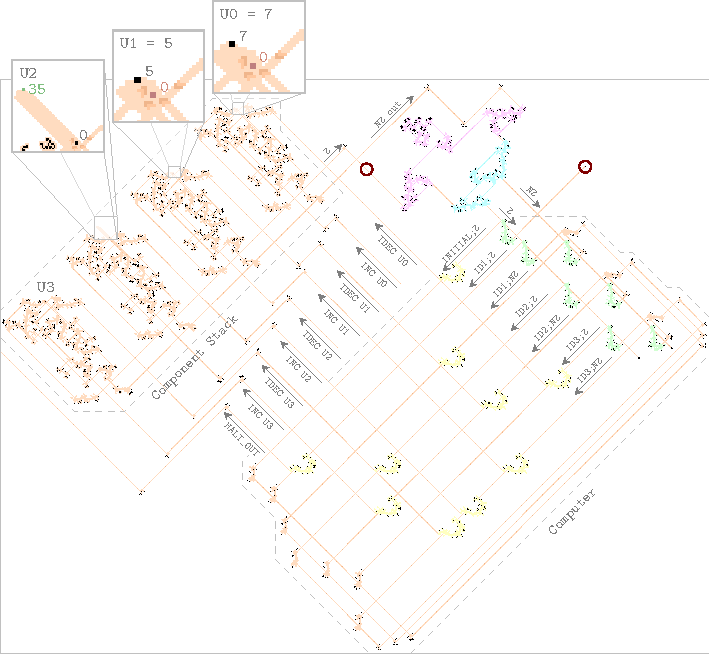
\includegraphics[width=\textwidth]{universal_computation/mult_computer.pdf}}
	\caption{A compiled Life pattern that multiplies the values of the registers \texttt{U0} and \texttt{U1} (which have been pre-loaded with the values \texttt{7} and \texttt{5}, respectively) and stores the result in \texttt{U2}, as in APGsembly~\ref{apg:mult_unary_reg}. The color scheme and general structure of this pattern is the same as in Figure~\ref{fig:add_computer}.}\label{fig:mult_computer}
\end{figure}

Just like we can multiply two registers via repeated addition, we can divide two registers via repeated subtraction. In particular, to compute the integer part of \texttt{U0 / U1} we can repeatedly subtract \texttt{U1} from \texttt{U0} until \texttt{U0 = 0}. The number of times that we were able to completely subtract \texttt{U1} is the integer part of \texttt{U0 / U1}, and the value that was contained in \texttt{U0} when we started our final subtraction is the remainder of that division. Implementing this division-by-subtraction algorithm in APGsembly is very similar to the multiplication-by-addition APGsembly~\ref{apg:mult_unary_reg}, so we leave it to Exercise~\ref{exer:division_by_subtraction}.

In fact, sliding block registers and the computational framework that we have introduced so far are already Turing complete---they can compute anything that can be computed. However, they are somewhat unwieldy to actually program to perform non-trivial computations, and they are not particularly interesting to look at. The remainder of this chapter is devoted to additional components that make computations in our Life patterns easier to implement, faster to perform, or simply more interesting to watch.


%%%%%%%%%%%%%%%%%%%%%%%%%%%%%%%%%%%%%%%%%%%%%%%%%%%%%%%%%%%%%%%%%%%%%%%%%
%%   SECTION: A BINARY REGISTER
%%%%%%%%%%%%%%%%%%%%%%%%%%%%%%%%%%%%%%%%%%%%%%%%%%%%%%%%%%%%%%%%%%%%%%%%%
\section{A Binary Register}\label{sec:binary_register}

One of the unfortunate features of sliding block registers is that the only actions they have available to them are addition and subtraction by \texttt{1}, so arithmetic operations involving large numbers stored in these registers take a long time to complete. For example, the addition code of APGsembly~\ref{alg:apgsembly_add_same_register} takes \texttt{U0+1} clock ticks to add the value of \texttt{U0} to \texttt{U1}, and the multiplication code of APGsembly~\ref{apg:mult_unary_reg} takes roughly \texttt{2 * U0 * U1} clock ticks to multiply \texttt{U0} by \texttt{U1}.\footnote{In fact, even the subtraction by \texttt{1} operation (i.e., \texttt{TDEC}) takes longer to complete if the value of the register is extremely large, since the sliding block takes longer to interact with and produce its return value when it is far away.}

While larger inputs leading to longer times to perform arithmetic operations is inevitable, we can save a lot of time by representing non-negative integers in a more efficient way than just as the position of a sliding block. While a sliding block register can be thought of as storing a non-negative integer in \textbf{unary}\index{unary} (i.e., the base-$1$ numeral system, in which each number is represented by tally marks or a distance from a fixed point), the register that we now introduce instead encodes non-negative integers in \textbf{binary} (i.e., the base-$2$ numeral system). Performing operations on such a register is somewhat more complicated, but it has the advantage of being much quicker because, for example, the non-negative integer $n$ can be stored in $\Theta(\log(n))$ space instead of $\Theta(n)$ space.%\footnote{Other bases larger than $2$ would also be quicker to work with than unary, but they would be even more complicated to implement.}

We call a register that stores a non-negative integer in this way a \textbf{binary register},\index{binary register} and the one that we make use of is displayed in Figure~\ref{fig:binary_register}. It uses block-moving shotguns similar to the ones in sliding block registers, except that they move a block~$6$ cells diagonally at a time instead of just~$1$. This wider spacing leaves room for additional reactions to place boats on one side of the sliding block. Every~$6$ cells along the sliding block's path is a designated bit location, which can contain either an empty space or a single boat, corresponding to the bits \texttt{0} and \texttt{1}, respectively.

\begin{figure}[!htb]
	\centering
	\embedlink{binary_register}{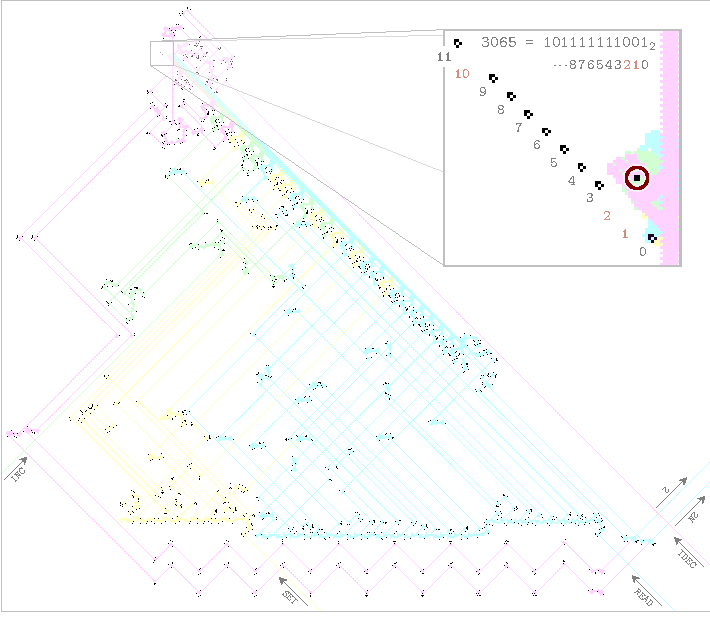
\includegraphics[width=\textwidth]{universal_computation/binary_register.pdf}}
	\caption{A binary register that uses a sliding block to keep track of the location of the read head (circled in \bgbox{redback}{red} in the zoom box at the ``\texttt{0}'' location) and boats to represent bits (shown here storing the value $3065 = 101111111001_2$). The sliding block and boat bits are manipulated by four different slow salvos corresponding to the register's four actions \texttt{INC}, \texttt{TDEC}, \texttt{READ}, and \texttt{SET}, which are generated by the circuitry highlighted in \bgbox{greenpastel}{green}, \bgbox{magentaback}{magenta}, \bgbox{aquaback}{aqua}, and \bgbox{yellowback2}{yellow}, respectively.}\label{fig:binary_register}
\end{figure}

The four actions available to this binary register are a bit more abstract than the actions of the sliding block register, since they work on the individual bits of the register rather than the value that those bits represent:\smallskip

\begin{itemize}
	\item An \texttt{INC}\index{INC} action moves the pointer block (called the \textbf{read head}\index{read head} of the register) to the next bit location, one step farther away.\smallskip
	
	\item A \texttt{TDEC}\index{TDEC} action moves the read head to the previous bit position (or keeps it in the same place if it's already at the zero position). This action also returns either \texttt{Z} or \texttt{NZ}, depending on whether or not the read head was already at the location of the least significant bit when this action was called.\footnote{This behavior is in complete analogy with the \texttt{TDEC} action for the sliding block register---it tests and \emph{then} it decrements (if possible). In fact, the \texttt{INC} and \texttt{TDEC} portions of the binary register from Figure~\ref{fig:binary_register} alone make up a sliding block register (they just manipulate the read head, not the boats that represent bits).}\smallskip
	
	\item A \texttt{READ}\index{READ} action sets the value of the bit at the current read head location to ``\texttt{0}''. This action returns either \texttt{Z} or \texttt{NZ}, depending on the original value of that bit.\smallskip
	
	\item Finally, a \texttt{SET}\index{SET} action places a ``\texttt{1}'' bit at the current read head location.\smallskip
\end{itemize}

Unlike a simple sliding block register, where there's no way to damage the mechanism by sending action signals to it, there are indeed ways to program a binary register that will cause it to explode catastrophically. In particular, if you send a \texttt{SET} action while there's already a \texttt{1} stored at the current read head location, it will cause irrecoverable damage. There's no built-in safety mechanism to prevent this, but this problem can easily be avoided by always sending a \texttt{READ} signal just before any \texttt{SET} signal.

We use \texttt{Bn} to denote the \texttt{n}-th binary register (where we start counting at \texttt{n = 0}), just like we use \texttt{Un} to denote the \texttt{n}-th sliding block register. To illustrate how to make use of these actions to perform bitwise operations, APGsembly~\ref{apg:store_139} shows how to store the value $139 = 10001011_2$ in a binary register \texttt{B0}.\footnote{The subscript ``$2$'' indicates that we are writing the number in binary.} Another way of storing the value $139$ in a binary register would be to change the appropriate line of the APGsembly header to \texttt{\#REGISTERS \{'B0':[0,'11010001']\}}. However, the header-based method only works if you want to set \texttt{B0} to $139$ at the start of the computation and not partway through it.
% NJ question for Dave: Is the #REGISTERS syntax for the B0 register above correct?

\begin{apgsembly}
	\begin{algorithmic}\small
		\State \verb|#COMPONENTS B0,NOP,HALT_OUT|
		\State \verb|#REGISTERS {}|
		\State \verb|# State    Input    Next state    Actions|
		\State \verb|# ---------------------------------------|
		\State \verb|INITIAL;   ZZ;      ID1;          SET B0, NOP|
		\State \verb|ID1;       ZZ;      ID2;          INC B0, NOP|
		\State \verb|ID2;       ZZ;      ID3;          SET B0, NOP|
		\State \verb|ID3;       ZZ;      ID4;          INC B0, NOP|
		\State \verb|ID4;       ZZ;      ID5;          INC B0, NOP|
		\State \verb|ID5;       ZZ;      ID6;          SET B0, NOP|
		\State \verb|ID6;       ZZ;      ID7;          INC B0, NOP|
		\State \verb|ID7;       ZZ;      ID8;          INC B0, NOP|
		\State \verb|ID8;       ZZ;      ID9;          INC B0, NOP|
		\State \verb|ID9;       ZZ;      ID10;         INC B0, NOP|
		\State \verb|ID10;      ZZ;      LSB1;         SET B0, NOP|
		\State
		\State \verb|# Move B0's read head back to its least significant bit.|
		\State \verb|LSB1;      ZZ;      LSB2;         TDEC B0|
		\State \verb|LSB2;      Z;       LSB2;         HALT_OUT|
		\State \verb|LSB2;      NZ;      LSB2;         TDEC B0|
	\end{algorithmic}
	\caption{APGsembly code for storing the value $139$ in the binary register \texttt{B0}, and then returning its read head to the least significant bit.}\label{apg:store_139}
\end{apgsembly}

This APGsembly also contains one new action that we have not yet seen: \texttt{NOP}.\index{NOP} This is an old standard programming abbreviation, short for ``\textbf{N}o \textbf{OP}eration''; it tells the computer not to change anything right now, but emit a \texttt{Z} return value anyway. It is typically used in conjunction with other actions that don't have a return value (\texttt{SET B0} and \texttt{INC B0} in this case), since exactly one action in every state's list of actions must return a value of either \texttt{Z} or \texttt{NZ}.\footnote{It may be tempting to merge multiple lines of APGsembly~\ref{apg:store_139} together so as to get rid of the \texttt{NOP} actions. For example, we might want to have an action list for a particular state that says something like \texttt{INC B0, INC B0, SET B0, NOP}. However, there are two problems with this: (1) we cannot call the same action twice in a single line of APGsembly (clock tick), and (2) it is not a good idea to perform two actions on the same register (\texttt{B0}) in the same clock tick. Indeed, it is not clear which one will be performed first (or even worse, they might interfere with each other and cause the register to self-destruct).}


%%%%%%%%%%%%%%%%%%%%%%%%%%%%%%%%%%%%%%%%%%%%%%%%%%%%%%%%%%%%%%%%%%%%%%%%%
%%   SECTION: A BINARY RULER
%%%%%%%%%%%%%%%%%%%%%%%%%%%%%%%%%%%%%%%%%%%%%%%%%%%%%%%%%%%%%%%%%%%%%%%%%
\subsection{A Binary Ruler}\label{sec:binary_ruler}

To illustrate how to perform some basic arithmetic operations with our binary register, consider the simple problem of increasing the value (i.e., the number that is stored in binary) of the register by~\texttt{1}. Unlike the sliding block register, there is no single action that performs this operation---we can only perform actions on one bit at a time, but increasing the value of a binary register by \texttt{1} may affect several of its bits due to carries.

Fortunately, since we are just increasing the value of the register by \texttt{1}, the carry bits are not difficult to take care of: we look for the least significant \texttt{0} bit and set it to \texttt{1}, and we set all bits that are less significant than it (which are necessarily currently equal to \texttt{1}) to \texttt{0}. Slightly more explicitly, we can increase the value of a binary register by \texttt{1} via the following procedure:\smallskip

\begin{enumerate}
	\item[1)] Start with the read head at the least significant bit and then proceed to step (2) below.\smallskip
	
	\item[2)] Read the value of the current bit (setting it equal to \texttt{0} in the process). If it equaled \texttt{0}, set it to \texttt{1} and then return the read head to the least significant bit. If it equaled \texttt{1}, move the read head to the next most significant bit (i.e., increase its position) and then return to step~(1).\smallskip
\end{enumerate}

This method is implemented in APGsembly~\ref{alg:apgsembly_binary_ruler}, which counts in binary by repeatedly adding \texttt{1} to the value of a binary register \texttt{B0}.\index{binary ruler}

\begin{apgsembly}
	\begin{algorithmic}\small
		\State \verb|#COMPONENTS B0,NOP|
		\State \verb|#REGISTERS {}|
		\State \verb|# State    Input    Next state    Actions|
		\State \verb|# ---------------------------------------|
		\State \verb|INITIAL;   ZZ;      CHECK1;       READ B0|
		\State
		\State \verb|## Determine whether the current bit equals 0 or 1.|
		\State \verb|# If it equals 0, set it to 1 and go to the least significant bit.|
		\State \verb|# If it equals 1, set it to 0 and go to the next most significant bit.|
		\State \verb|CHECK1;    Z;       LSB1;         SET B0, NOP|
		\State \verb|CHECK1;    NZ;      CHECK2;       INC B0, NOP|
		\State \verb|CHECK2;    ZZ;      CHECK1;       READ B0|
		\State
		\State \verb|# Move B0's read head back to its least significant bit.|
		\State \verb|LSB1;      ZZ;      LSB2;         TDEC B0|
		\State \verb|LSB2;      Z;       CHECK1;       READ B0|
		\State \verb|LSB2;      NZ;      LSB2;         TDEC B0|
	\end{algorithmic}
	\caption{APGsembly code for a \textbf{binary ruler}---a pattern that counts in binary.}\label{alg:apgsembly_binary_ruler}
\end{apgsembly}

One interesting feature of the pattern that results from compiling this APGsembly code (see Figure~\ref{fig:binary_ruler}) is that it exhibits a new type of slow growth that we have not yet seen. We explored patterns with slowly-growing \emph{population} in Section~\ref{sec:irreg_guns}, but this pattern instead has a slowly-growing \emph{bounding box}.\index{bounding box} In particular, its \textbf{diameter}\index{diameter} (i.e., its longest bounding box side length) in generation~$t$ is $\Theta(\log(t))$, since this is the rate at which new most significant bits are added to the end of the binary register.

\begin{figure}[!htb]
	\centering
	\embedlink{binary_ruler}{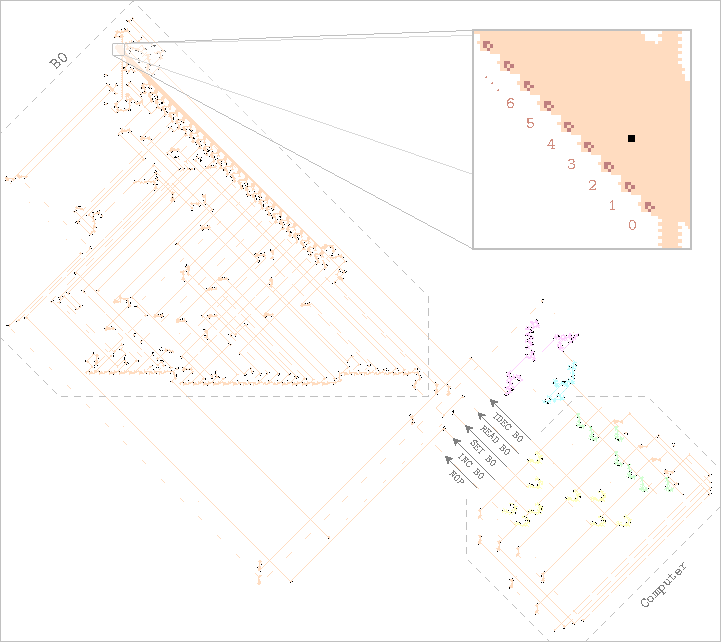
\includegraphics[width=\textwidth]{universal_computation/binary_ruler.pdf}}
	\caption{A \textbf{binary ruler} that counts in binary via APGsembly~\ref{alg:apgsembly_binary_ruler}. As a result, it grows very slowly, with its diameter in generation~$t$ being $\Theta(\log(t))$. Its component stack consists of just a single component---the binary register \texttt{B0}, which places boats that act as bits in the locations highlighted in \bgbox{redback}{red}.}\label{fig:binary_ruler}
\end{figure}

This diametric growth rate is much slower than any other unbounded pattern that we have seen so far (all of which have been $\Theta(t)$). We will return to this idea of patterns with slowly-growing bounding boxes, and push it to its ultimate limit, in Section~\ref{sec:Osqrtlogt}.


%%%%%%%%%%%%%%%%%%%%%%%%%%%%%%%%%%%%%%%%%%%%%%%%%%%%%%%%%%%%%%%%%%%%%%%%%
%%   SECTION: BINARY ADDITION AND SUBTRACTION
%%%%%%%%%%%%%%%%%%%%%%%%%%%%%%%%%%%%%%%%%%%%%%%%%%%%%%%%%%%%%%%%%%%%%%%%%
\subsection{Addition, Subtraction, and Multiplication by 10}\label{sec:add_sub_and_mult10}\index{ADD component}\index{SUB component}

While addition and subtraction of values that are stored in sliding block (unary) registers is reasonably straightforward (refer back to Section~\ref{sec:compiled_add_two_registers}), these operations are more complicated for binary registers. Even just adding \texttt{1} to the value of a binary register and then resetting its read head makes use of seven lines of code (refer back to APGsembly~\ref{alg:apgsembly_binary_ruler}). The reason for the increase in complexity in this case is that when we add or subtract two binary numbers, we have to keep track of bits that are carried from one bit to the next, possibly many times in a row.

In order to make these arithmetic operations easier to perform, we introduce additional components that are custom-made for storing carry bits. In particular, the \texttt{ADD} and \texttt{SUB} components displayed in Figures~\ref{fig:add_component} and~\ref{fig:sub_component}, respectively, perform bitwise operations to assist in the addition and subtraction of binary registers.\footnote{These components were designed in 2009 or so, before the discovery of the Snark or the syringe. If desired, they could be rebuilt much smaller nowadays with modern Life technology.} The \texttt{ADD} component performs the addition of two bits, outputting the least significant bit of the addition and storing the carry bit in its own internal memory, and the \texttt{SUB} component similarly performs the subtraction of two bits while keeping track of the borrow bit.\footnote{Unlike the sliding block and binary registers, we only ever need one \texttt{ADD} or \texttt{SUB} component. In fact, every component that we see from this point on is limited to just a single copy per Life pattern---the sliding block and binary registers are the only components that we can use multiple copies of.}

\begin{figure}[!htb]
	\centering
	\begin{minipage}[t]{0.48\textwidth}
		\centering
		\embedlink{add_component}{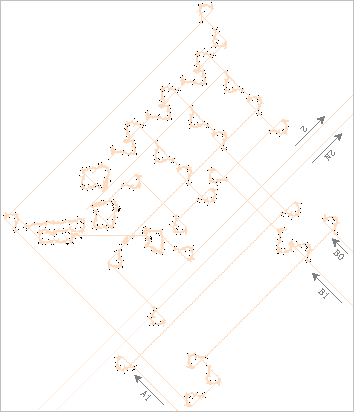
\includegraphics[width=\textwidth]{universal_computation/add_component.pdf}}
		\caption{The \texttt{ADD} component. To add up two bits \texttt{x} and \texttt{y} while respecting carry bits, input \texttt{A1} if \texttt{x = 1} (provide no input if \texttt{x = 0}) and then \texttt{By}.}\label{fig:add_component}
	\end{minipage}\hfill
	\begin{minipage}[t]{0.48\textwidth}
		\centering
		\embedlink{sub_component}{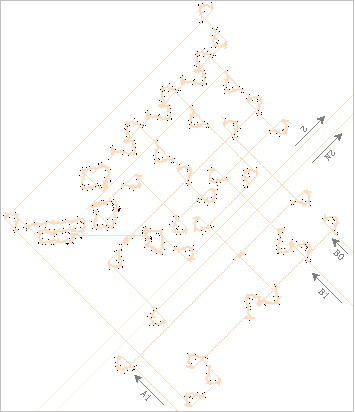
\includegraphics[width=\textwidth]{universal_computation/sub_component.pdf}}
		\caption{The \texttt{SUB} component. To subtract a bit \texttt{y} from \texttt{x} while respecting carry bits, input \texttt{A1} if \texttt{x = 1} (provide no input if \texttt{x = 0}) and then \texttt{By}.}\label{fig:sub_component}
	\end{minipage}
\end{figure}

More specifically, if we use \texttt{z} to denote the bit that is currently stored in the internal memory of the \texttt{ADD} component, then feeding two bits \texttt{x} and \texttt{y} into it returns a value of \texttt{(x + y + z) mod 2} and updates its memory to the value \texttt{(x + y + z)/2} (where we mean integer division here, so that this memory value is either \texttt{0} and \texttt{1}). This \texttt{ADD} component can then be used to add up the values stored in binary registers by repeatedly calling upon it to add up the least-significant bits of those registers, then their next-least-significant bits, and so on until all bits have been added.

However, this procedure only works if we know where the most significant bit is, so that we know when we can stop performing this bitwise addition. The binary registers themselves provide no such functionality---even if we find a million ``\texttt{0}'' bits in a row, there could always be a more significant ``\texttt{1}'' bit waiting to be found further on. For this reason, when performing bitwise arithmetic operations like addition and subtraction, we need to make use of a helper sliding block register that tells us (an upper bound of) how many bits the binary registers are making use of. The contents of this sliding block register needs to be updated as our computation proceeds to make sure that it always allocates enough bits of memory to the binary registers.

The way that the bit addition \texttt{x + y} is executed via APGsembly is that the pair of commands \texttt{ADD~Ax} and then \texttt{ADD~By} must be called (where we replace \texttt{x} and \texttt{y} by their actual binary values, as in \texttt{ADD B1}, for example).\footnote{Be careful: this means that \texttt{B0} and \texttt{B1} can be both components (as in \texttt{INC B0} or \texttt{READ B1}) and actions (as in \texttt{ADD B0}).} The \texttt{ADD Ax} command does not return an output (it just adds the input bit to the internal memory), but the \texttt{ADD By} command does (so it should always be used second). Furthermore, the \texttt{ADD A0} command is not actually implemented, since it does nothing---it does not return a value and also does not alter the internal memory.\footnote{This contrasts with the command \texttt{ADD B0}, which also does not alter the internal memory, but \emph{does} return a value. In particular, \texttt{ADD B0} returns the contents of the internal memory and then resets that memory to \texttt{0}.}

For example, to add binary registers containing the numbers $104 = 1101000_2$ and $57 = 111001_2$, we could perform the following sequence of actions in APGsembly (where we perform the ``\texttt{A}'' action in the top row and then the ``\texttt{B}'' action directly below it before moving left-to-right):
\begin{center}
	\begin{tabular}{llllllll}
		\leavevmode\hphantom{\texttt{ADD A0}} \ & \hphantom{\texttt{ADD A0}} \ & \hphantom{\texttt{ADD A0}} \ & \texttt{ADD A1} \ & \hphantom{\texttt{ADD A0}} \ & \texttt{ADD A1} \ & \texttt{ADD A1} \ & \hphantom{\texttt{ADD A0}} \\
		\texttt{ADD B1}, \ & \texttt{ADD B0}, \ & \texttt{ADD B0}, \ & \texttt{ADD B1}, \ & \texttt{ADD B1}, \ & \texttt{ADD B1}, \ & \texttt{ADD B0}, \ & \texttt{ADD B0}.
	\end{tabular}
\end{center}
Notice that these \texttt{ADD} actions are performed ``backwards'': they start from the least significant bits of the numbers that we are adding. Also, we need to append an extra \texttt{ADD B0} command at the very end to account for the fact that the sum may have one more bit than the summands.\footnote{Another reason that it is a good idea to call \texttt{ADD B0} after adding two registers is that it clears the internal memory of the \texttt{ADD} component.} These actions would return the outputs
\begin{center}
	\begin{tabular}{llllllll}
		\leavevmode\hphantom{\texttt{CD}}\texttt{NZ},\hphantom{\texttt{CD}} \ & \hphantom{\texttt{AB}}\texttt{Z},\hphantom{\texttt{CDE}} \ & \hphantom{\texttt{AB}}\texttt{Z},\hphantom{\texttt{CDE}} \ & \hphantom{\texttt{AB}}\texttt{Z},\hphantom{\texttt{CDE}} \ & \hphantom{\texttt{AB}}\texttt{Z},\hphantom{\texttt{CDE}} \ & \hphantom{\texttt{AB}}\texttt{NZ},\hphantom{\texttt{CD}} \ & \hphantom{\texttt{AB}}\texttt{Z},\hphantom{\texttt{CDE}} \ & \hphantom{\texttt{AB}}\texttt{NZ}\hphantom{\texttt{CD}}
	\end{tabular}
\end{center}
corresponding to the fact that $104 + 57 = 161 = 10100001_2$. Complete APGsembly that implements this addition of two binary registers is provided in APGsembly~\ref{alg:apgsembly_binary_add_sub}.

\begin{apgsembly}
	\centering
	\begin{minipage}[t]{.49\textwidth}
		\begin{algorithmic}\tiny
			\State \verb|#COMPONENTS B0-1,U0-2,ADD,NOP,HALT_OUT|
			\State \verb|#REGISTERS {'B0':[0,'0001011'], 'B1':[0,'100111'], 'U0':8}|
			\State \verb|# State    Input    Next state    Actions|
			\State \verb|# ---------------------------------------|
			\State \verb|INITIAL;   ZZ;      ADD1;         TDEC U0|
			\State \verb||
			\State \verb|# Copy U0 into U2, with the help of U1|
			\State \verb|ADD1;      Z;       ADD2;         TDEC U1|
			\State \verb|ADD1;      NZ;      ADD1;         TDEC U0, INC U1|
			\State \verb|ADD2;      Z;       ADD3;         TDEC U2|
			\State \verb|ADD2;      NZ;      ADD2;         TDEC U1, INC U0, INC U2|
			\State \verb||
			\State \verb|# Loop over U2 to add B1 to B0, one bit at a time.|
			\State \verb|ADD3;      Z;       ADD7;         TDEC B0|
			\State \verb|ADD3;      NZ;      ADD4;         READ B0|
			\State \verb|ADD4;      Z;       ADD5;         READ B1|
			\State \verb|ADD4;      NZ;      ADD5;         READ B1, ADD A1|
			\State \verb|ADD5;      Z;       ADD6;         ADD B0|
			\State \verb|ADD5;      NZ;      ADD6;         ADD B1, SET B1|
			\State \verb|ADD6;      Z;       ADD3;         TDEC U2, INC B0, INC B1|
			\State \verb|ADD6;      NZ;      ADD6;         SET B0, NOP|
			\State \verb||
			\State \verb|# Move the B0 and B1 read heads back to least significant bit.|
			\State \verb|ADD7;      Z;       ADD8;         TDEC B1|
			\State \verb|ADD7;      NZ;      ADD7;         TDEC B0|
			\State \verb|ADD8;      Z;       ADD8;         HALT_OUT|
			\State \verb|ADD8;      NZ;      ADD8;         TDEC B1|
		\end{algorithmic}
	\end{minipage}\hfill{\color{gray}\vline}\hfill
	\begin{minipage}[t]{.49\textwidth}
		\begin{algorithmic}\tiny
			\State \verb|#COMPONENTS B0-1,U0-2,SUB,NOP,HALT_OUT|
			\State \verb|#REGISTERS {'B0':[0,'0001011'], 'B1':[0,'100111'], 'U0':8}|
			\State \verb|# State    Input    Next state    Actions|
			\State \verb|# ---------------------------------------|
			\State \verb|INITIAL;   ZZ;      SUB1;         TDEC U0|
			\State \verb||
			\State \verb|# Copy U0 into U2, with the help of U1|
			\State \verb|SUB1;      Z;       SUB2;         TDEC U1|
			\State \verb|SUB1;      NZ;      SUB1;         TDEC U0, INC U1|
			\State \verb|SUB2;      Z;       SUB3;         TDEC U2|
			\State \verb|SUB2;      NZ;      SUB2;         TDEC U1, INC U0, INC U2|
			\State \verb||
			\State \verb|# Loop over U2 to subtract B1 from B0, one bit at a time.|
			\State \verb|SUB3;      Z;       SUB7;         TDEC B0|
			\State \verb|SUB3;      NZ;      SUB4;         READ B0|
			\State \verb|SUB4;      Z;       SUB5;         READ B1|
			\State \verb|SUB4;      NZ;      SUB5;         READ B1, SUB A1|
			\State \verb|SUB5;      Z;       SUB6;         SUB B0|
			\State \verb|SUB5;      NZ;      SUB6;         SUB B1, SET B1|
			\State \verb|SUB6;      Z;       SUB3;         TDEC U2, INC B0, INC B1|
			\State \verb|SUB6;      NZ;      SUB6;         SET B0, NOP|
			\State \verb||
			\State \verb|# Move the B0 and B1 read heads back to least significant bit.|
			\State \verb|SUB7;      Z;       SUB8;         TDEC B1|
			\State \verb|SUB7;      NZ;      SUB7;         TDEC B0|
			\State \verb|SUB8;      Z;       SUB8;         HALT_OUT|
			\State \verb|SUB8;      NZ;      SUB8;         TDEC B1|
		\end{algorithmic}
	\end{minipage}
	\caption{APGsembly code for adding (left) or subtracting (right) the binary register \texttt{B1} to/from \texttt{B0}. In both cases, the new value is stored in \texttt{B0} while the value of \texttt{B1} is unaffected. The number of bits allocated to the binary registers is stored in \texttt{U0}, and the registers \texttt{U1} and \texttt{U2} are only used temporarily (they start at, and are returned to, a value of \texttt{0}).}\label{alg:apgsembly_binary_add_sub}
\end{apgsembly}

Since the \texttt{ADD} component is somewhat technical and basically only has a single use, not much is lost if we do not actually understand its inner workings and just accept APGsembly~\ref{alg:apgsembly_binary_add_sub} as a black box that adds up two binary registers. Similarly, we do not go into any great depth in explaining the inner working of the \texttt{SUB} component. Instead, we just note that it does for subtraction exactly what the \texttt{ADD} component does for addition---it keeps track of the borrow bit (which is analogous to the carry bit for addition) and thus lets us subtract binary registers from each other one bit at a time. The resulting APGsembly code for subtracting one binary register from another one is also provided in APGsembly~\ref{alg:apgsembly_binary_add_sub}. Note that this code for subtracting \texttt{B1} from \texttt{B0} assumes that \texttt{B1 <= B0}; if you are unsure of which binary register is the smaller one then you should first compare them (see Exercise~\ref{exer:universal_computation_apgsembly_binary_compare}).

Now that we know how to add and subtract binary components, we can also multiply and divide them via the same tricks that we used for sliding block registers in Section~\ref{sec:multiply_two_registers} and Exercise~\ref{exer:division_by_subtraction}. That is, we simply add or subtract repeatedly (see Exercise~\ref{exer:universal_computation_apgsembly_multiply_binary}). However, doing so can be quite time-consuming when the registers store large values, so we now introduce one additional \index{MUL component} custom binary register arithmetic component---one that helps us multiply a binary register by $10$.\footnote{The reason for us making $10$ easier to multiply by (as opposed to any other fixed integer) is that multiplication by $10$ is a common operation when working with decimal numbers. In particular, we will make use of this multiplication-by-$10$ component to help us extract digits in the upcoming $\pi$~calculator in Section~\ref{sec:pi_calc}.}

This final new component is called \texttt{MUL}, which stores \emph{four} carry bits so that we can multiply a binary register by $10$ one bit at a time, just like the \texttt{ADD} and \texttt{SUB} components made use of a single memory bit to let us add and subtract binary registers one bit at a time.\footnote{The internal memory of these \texttt{ADD}, \texttt{SUB}, and \texttt{MUL} components is actually slightly more complicated than we have indicated. For example, the \texttt{ADD} component has \emph{two} bits of internal memory since between the \texttt{Ax} call (if any) and the \texttt{By} call, it tracks the carry bit and the \texttt{A} input value separately. Those values cannot be combined and stored in a single one-bit memory cell, because an internal \texttt{A0+(0 carry bit)} results in a different internal state than \texttt{A1+(1 carry bit)}, even though they both have a \texttt{Z} output.} The \texttt{MUL} component is displayed in Figure~\ref{fig:mul_component}, though it is not very enlightening to look at.\footnote{Even moreso than the binary register and \texttt{ADD} and \texttt{SUB} components, the \texttt{MUL} component could be made significantly smaller via modern machinery like Snarks and syringes.}

\begin{figure}[!htb]
	\centering
	\embedlink{mul_component}{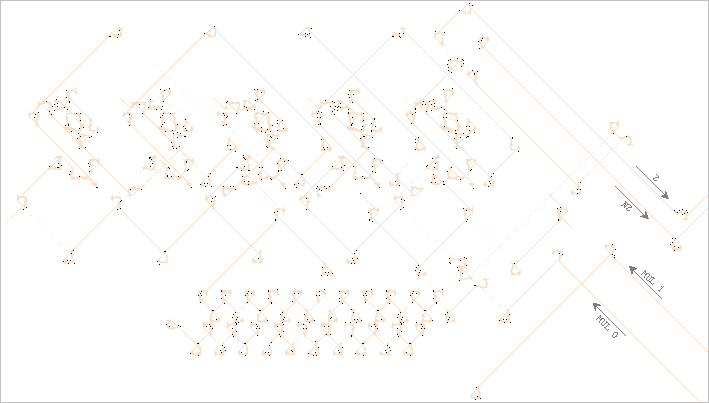
\includegraphics[width=\textwidth]{universal_computation/mul_component.pdf}}
	\caption{The \texttt{MUL} component, which keeps track of multiple carry bits so as to help us easily multiply a binary register by $10$.}\label{fig:mul_component}
\end{figure}

This component is called in APGsembly via the commands \texttt{MUL 0} and \texttt{MUL 1}, where the number after the name of the component refers to the current bit of the binary register that we are multiplying by $10$. For example, to multiply the number $26 = 11010_2$ by $10$, we could perform the following sequence of actions in APGsembly:
\begin{center}
	\texttt{MUL 0}, \ \ \texttt{MUL 1}, \ \ \texttt{MUL 0}, \ \ \texttt{MUL 1}, \ \ \texttt{MUL 1}, \ \ \texttt{MUL 0}, \ \ \texttt{MUL 0}, \ \ \texttt{MUL 0}, \ \ \texttt{MUL 0}.
\end{center}
These \texttt{MUL} actions also start from the least significant bit of the number that we are multiplying by $10$, just like the \texttt{ADD} and \texttt{SUB} actions. Also, we need to append enough \texttt{MUL 0} commands in order to retrieve the extra bits that the output will have. Four extra \texttt{MUL 0} commands always suffices, and these actions would return the outputs
\begin{center}
	\leavevmode\hphantom{\texttt{ABCD}}\texttt{Z}, \ \ \hphantom{\texttt{ABCD}}\texttt{Z}, \ \ \hphantom{\texttt{ABC}}\texttt{NZ}, \ \ \hphantom{\texttt{ABCD}}\texttt{Z}, \ \ \hphantom{\texttt{ABCD}}\texttt{Z}, \ \ \hphantom{\texttt{ABCD}}\texttt{Z}, \ \ \hphantom{\texttt{ABCD}}\texttt{Z}, \ \ \hphantom{\texttt{ABCD}}\texttt{Z}, \ \ \hphantom{\texttt{ABC}}\texttt{NZ},\hphantom{\texttt{ABCD}}
\end{center}
corresponding to the fact that $26 \times 10 = 260 = 100000100_2$.

We can thus now multiply a binary register by $10$ via approximately the same number of lines of APGsembly code as were required to add and subtract the values of binary registers. Complete APGsembly code for carrying out this multiplication is provided in APGsembly~\ref{alg:apgsembly_mul_ten}.

\begin{apgsembly}
	\begin{algorithmic}\small
		\State \verb|#COMPONENTS B0,U0-2,MUL,NOP,HALT_OUT|
		\State \verb|#REGISTERS {'B0':[0,'01011'], 'U0':9}|
		\State \verb|# State    Input    Next state    Actions|
		\State \verb|# ---------------------------------------|
		\State \verb|INITIAL;   ZZ;      MUL1;         TDEC U0|
		\State \verb||
		\State \verb|# Copy U0 into U2, with the help of U1|
		\State \verb|MUL1;      Z;       MUL2;         TDEC U1|
		\State \verb|MUL1;      NZ;      MUL1;         TDEC U0, INC U1|
		\State \verb|MUL2;      Z;       MUL3;         TDEC U2|
		\State \verb|MUL2;      NZ;      MUL2;         TDEC U1, INC U0, INC U2|
		\State \verb||
		\State \verb|# Loop over U2 to multiply B0 by 10, one bit at a time.|
		\State \verb|MUL3;      Z;       MUL6;         TDEC B0|
		\State \verb|MUL3;      NZ;      MUL4;         READ B0|
		\State \verb|MUL4;      Z;       MUL5;         MUL 0|
		\State \verb|MUL4;      NZ;      MUL5;         MUL 1|
		\State \verb|MUL5;      Z;       MUL3;         TDEC U2, INC B0|
		\State \verb|MUL5;      NZ;      MUL5;         SET B0, NOP|
		\State \verb||
		\State \verb|# Move the B0 read head back to its least significant bit.|
		\State \verb|MUL6;      Z;       MUL6;         HALT_OUT|
		\State \verb|MUL6;      NZ;      MUL6;         TDEC B0|
	\end{algorithmic}
	\caption{APGsembly code for multiplying the binary register \texttt{B0} by \texttt{10}. The number of bits allocated to \texttt{B0} is stored in \texttt{U0}, and the registers \texttt{U1} and \texttt{U2} are only used temporarily (they start at, and are returned to, a value of \texttt{0}). Compare with APGsembly~\ref{alg:apgsembly_binary_add_sub} for addition and subtraction.}\label{alg:apgsembly_mul_ten}
\end{apgsembly}


%%%%%%%%%%%%%%%%%%%%%%%%%%%%%%%%%%%%%%%%%%%%%%%%%%%%%%%%%%%%%%%%%%%%%%%%%
%%   SECTION: CHARACTER PRINTER
%%%%%%%%%%%%%%%%%%%%%%%%%%%%%%%%%%%%%%%%%%%%%%%%%%%%%%%%%%%%%%%%%%%%%%%%%
\section{A Character Printer}\label{sec:decimal_printer}\index{character printer}

We now demonstrate how to construct a component that is capable of printing any characters (e.g., digits or letters) of our choosing on the Life plane, in a font made up of blocks. Fortunately, we have already seen most of the reactions that we need to assemble a printer of this type. Very much along the same lines as the binary register of the previous section, our character printer will use a variant of slide gun technology to move a block that marks the current cursor position. We will also need a reaction that can use that cursor block to place another block nearby to serve as the pixels in printed characters (much like the read head block in the binary register can be used to place boats nearby to serve as bits in the register's memory).

In order to make our printer somewhat simpler to construct, we will have it move and position blocks via slow salvos like the ones that we introduced back in Section~\ref{sec:slow_salvo}. Doing this lets us not have to worry about the precise timing of the gliders that we use to move and duplicate blocks---we just have to position them correctly (which is trivial via an array of edge-shooting Herschel conduits). This is the same technique that we used to construct the binary register in Figure~\ref{fig:binary_register}, which has a long diagonal line of $26$~edge shooters along its northeast edge.

One particular salvo for placing a pixel block is displayed in Figure~\ref{fig:char_printer_place_pixel}. While this salvo is not quite slow (the first $3$ of its $7$ gliders must be synchronized, and the $4$th glider must have the correct mod~$8$ timing), it has the added benefit of being unidirectional.\footnote{We have already seen the slow portion of this salvo---the first slow glider is the $(2,1)$ block pull from Figure~\ref{fig:glider_block_move}, and the second and third gliders duplicate the block as in Figure~\ref{fig:slow_salvo_splitter}. The first four (synchronized) gliders just reposition the cursor block so that these later (slow) gliders, when duplicating the block, move it back to where it started.} Similarly, Figure~\ref{fig:char_printer_push_cursor} shows a 14-glider unidirectional slow salvo that pushes the cursor block 32 full diagonals farther away from the glider source. Importantly, this cursor-pushing reaction can be used regardless of whether or not the pixel-placing reaction was used, since the pixel is placed in a location that is never touched by the cursor-pushing reaction.

\begin{figure}[!htb]
	\centering
	\begin{subfigure}{\textwidth}
		\centering
		\embedlink{char_printer_place_pixel}{\vcenteredhbox{\patternimg{0.08}{char_printer_place_pixel_0}}} \vcenteredhbox{\genarrow{138}} \raisebox{-0.48\height}{\begin{tikzpicture}[scale=0.5, every node/.style={transform shape}]%
			\node[inner sep=0pt,anchor=south west] at (0,0) {\patternlink{char_printer_place_pixel}{\patternimg{0.16}{char_printer_place_pixel_138}}};
			
			\colorletternode{green}{5.07}{0.84}{1}
			\colorletternode{green}{5.75}{1.8}{2}
			\colorletternode{green}{3.6}{1.95}{3}
			\end{tikzpicture}} \vcenteredhbox{\gliderarrow{3}} \patternlink{char_printer_place_pixel}{\vcenteredhbox{\patternimg{0.08}{char_printer_place_pixel_141}}}
		\caption{A $7$-glider salvo that uses $4$ synchronized gliders and then $3$ slow gliders to create a far-away block, while only temporarily disturbing the target (cursor) block.}\label{fig:char_printer_place_pixel}
	\end{subfigure}\\[0.2cm]
	\begin{subfigure}{\textwidth}
		\centering
		\raisebox{-0.48\height}{\begin{tikzpicture}[scale=0.5, every node/.style={transform shape}]%
			\node[inner sep=0pt,anchor=south west] at (0,0) {\embedlink{char_printer_push_cursor}{\patternimg{0.234}{char_printer_push_cursor_0}}};
			
			\colorletternode{green}{4.55}{5.7}{1}
			\colorletternode{green}{3.7}{4.75}{2}
			\colorletternode{green}{3.05}{4.45}{3}
			\colorletternode{green}{0.55}{3.1}{4}
			\colorletternode{green}{1.9}{3.8}{5}
			\colorletternode{green}{2.9}{6.05}{6}
			\colorletternode{green}{2.7}{6.7}{7}
			\end{tikzpicture}} \vcenteredhbox{\gliderarrow{7}} \raisebox{-0.48\height}{\begin{tikzpicture}[scale=0.5, every node/.style={transform shape}]%
			\node[inner sep=0pt,anchor=south west] at (0,0) {\patternlink{char_printer_push_cursor}{\patternimg{0.234}{char_printer_push_cursor_7}}};
			
			\colorletternode{green}{6.05}{4.25}{1}
			\colorletternode{green}{5.4}{4.5}{2}
			\colorletternode{green}{4.85}{2.9}{3}
			\colorletternode{green}{4.8}{4.55}{4}
			\colorletternode{green}{3.2}{5}{5}
			\colorletternode{green}{3.05}{5.95}{6}
			\colorletternode{green}{3.1}{3.7}{7}
			\end{tikzpicture}} \vcenteredhbox{\gliderarrow{7}} \patternlink{char_printer_push_cursor}{\vcenteredhbox{\patternimg{0.117}{char_printer_push_cursor_14}}}
		\caption{A $14$-glider p$2$ slow salvo that pushes the target (cursor) block $32$~full diagonals away, while avoiding the location of the hypothetical printed pixel from~(a).}\label{fig:char_printer_push_cursor}
	\end{subfigure}
	\caption{Glider salvos that can be used to print block pixels at a separation of $32$~full diagonals.}\label{fig:char_printer_salvos}
\end{figure}

To create the salvos that implement these pixel-printing and cursor-moving operations, we just use stable circuitry like Snarks, syringes, and the edge-shooting Herschel conduits that we saw in Chapter~\ref{chp:stationary_circuitry}. If we want the next pixel in the current row to be empty, we just push the cursor block by creating the glider salvo from Figure~\ref{fig:char_printer_push_cursor}. If we want to print the next pixel in the current row, we instead create the salvo from Figure~\ref{fig:char_printer_place_pixel} and \emph{then} trigger the cursor-pushing mechanism. A device called a \textbf{row printer}\index{row printer} that implements both of these operations is displayed in Figure~\ref{fig:row_printer}.

\begin{figure}[!htb]
	\centering
	\embedlink{row_printer}{\includegraphics[width=\textwidth]{universal_computation/row_printer.pdf}}
	\caption{A \textbf{row printer} that can be used to either push a cursor block forward by $32$ full diagonals (highlighted in \bgbox{orangeback2}{orange}), or print a pixel block (highlighted in \bgbox{greenpastel}{green}) and \emph{then} push the cursor block.}\label{fig:row_printer}
\end{figure}

This row printer lets us easily print an arbitrary sequence of pixels (blocks) along a single (northwest-to-southeast diagonal) row. To construct a more general printer that lets us print characters that are several pixels tall, we simply use multiple row printers---one cursor block and one row printer per pixel of height in the characters. For example, if we wish to print characters that are $10$~pixels tall, we use $10$ cursor blocks that are offset from each other diagonally in the southwest-to-northeast direction, and we aim a separate row printer at each of them.

The end result of using multiple row printers in this way is that each row always advances its cursor block by the same distance ($32$ full diagonals), regardless of whether or not a pixel has been placed in that row. Instructions for which pixels to print in each row (and thus which characters to print overall) can be encoded straightforwardly in circuitry that sends a glider into the appropriate input slot of each row printer. To illustrate this idea, Figure~\ref{fig:abracadabra_printer} presents a pattern that is capable of printing the characters \texttt{A}, \texttt{B}, \texttt{C}, \texttt{D}, and \texttt{R} in a font made up of blocks, and which has had $11$ glider signals fed into it, instructing it to print the word ``\texttt{ABRACADABRA}''.

\begin{figure}[!htb]
	\centering
	\embedlink{abracadabra_printer}{\includegraphics[width=\textwidth]{universal_computation/abracadabra_printer.pdf}}
	\caption{A printer with five input glider lanes that direct it to print one of the letters \texttt{A}, \texttt{B}, \texttt{C}, \texttt{D}, or \texttt{R} in a font made up of blocks, shown here having already printed the word ``\texttt{ABRACADABRA}''. The font used is $8$ pixels (blocks) high, so $8$ row printers and $8$ cursor blocks (circled in \bgbox{redback}{red}) are used. The row printer highlighted in \bgbox{yellowback2}{yellow} takes care of all printing on the second-from-the-top row, for example. The rectangular array of splitters below the row printers encodes which pixels should be printed in each row. For example, the arrangement of splitters highlighted in \bgbox{aquaback}{aqua} encodes which pixels should be printed by each row printer when an ``\texttt{A}'' input is received.}\label{fig:abracadabra_printer}
\end{figure}

This very simple printer design adapts readily to any character height or width, and any number of characters.\footnote{A script that builds a printer pattern for any specified set of characters can be downloaded from \httpsurl{conwaylife.com/forums/viewtopic.php?p=93420\#p93420}.} There is no requirement that all characters have the same width. They are technically all the same height, though they may appear to be different heights if some characters are padded with empty pixels at the top or bottom.

While APGsembly requires us to explicitly specify which digit we want to print (e.g., we cannot print the contents of a sliding block register \texttt{U0} via the command \texttt{OUTPUT U0}), we can get around this limitation by repeatedly \texttt{TDEC}ing that register to determine its value, and then printing out that value. This idea is made explicit by APGsembly~\ref{alg:apgsembly_print_sbr}. Note that this APGsembly requires that \texttt{U0} is storing a value between $0$ and $9$, inclusive, but it could be modified straightforwardly to handle any fixed upper bound just by adding additional \texttt{TDEC} statements. It is even possible to print the contents of a sliding block register regardless of how many decimal digits it has, but this is much more complicated---see Exercise~\ref{exer:universal_computation_print_register}.

\begin{apgsembly}
	\begin{algorithmic}\small
		\State \verb|#COMPONENTS U0,OUTPUT,HALT_OUT|
		\State \verb|#REGISTERS {'U0':7}|
		\State \verb|# State    Input    Next state    Actions|
		\State \verb|# ---------------------------------------|
		\State \verb|INITIAL;   ZZ;      OUT0;         TDEC U0|
		\State \verb|OUT0;      Z;       OUT0;         OUTPUT 0, HALT_OUT|
		\State \verb|OUT0;      NZ;      OUT1;         TDEC U0|
		\State \verb|OUT1;      Z;       OUT1;         OUTPUT 1, HALT_OUT|
		\State \verb|OUT1;      NZ;      OUT2;         TDEC U0|
		\State \verb|OUT2;      Z;       OUT2;         OUTPUT 2, HALT_OUT|
		\State \verb|OUT2;      NZ;      OUT3;         TDEC U0|
		\State \verb|OUT3;      Z;       OUT3;         OUTPUT 3, HALT_OUT|
		\State \verb|OUT3;      NZ;      OUT4;         TDEC U0|
		\State \verb|OUT4;      Z;       OUT4;         OUTPUT 4, HALT_OUT|
		\State \verb|OUT4;      NZ;      OUT5;         TDEC U0|
		\State \verb|OUT5;      Z;       OUT5;         OUTPUT 5, HALT_OUT|
		\State \verb|OUT5;      NZ;      OUT6;         TDEC U0|
		\State \verb|OUT6;      Z;       OUT6;         OUTPUT 6, HALT_OUT|
		\State \verb|OUT6;      NZ;      OUT7;         TDEC U0|
		\State \verb|OUT7;      Z;       OUT7;         OUTPUT 7, HALT_OUT|
		\State \verb|OUT7;      NZ;      OUT8;         TDEC U0|
		\State \verb|OUT8;      Z;       OUT8;         OUTPUT 8, HALT_OUT|
		\State \verb|OUT8;      NZ;      OUT8;         OUTPUT 9, HALT_OUT|
	\end{algorithmic}
	\caption{APGsembly code for printing the contents of the sliding block register \texttt{U0}, which is assumed to contain a value between \texttt{0} and \texttt{9} inclusive, and setting \texttt{U0 = 0} at the same time.}\label{alg:apgsembly_print_sbr}
\end{apgsembly}



%%%%%%%%%%%%%%%%%%%%%%%%%%%%%%%%%%%%%%%%%%%%%%%%%%%%%%%%%%%%%%%%%%%%%%%%%
%%   SECTION: PI CALCULATOR
%%%%%%%%%%%%%%%%%%%%%%%%%%%%%%%%%%%%%%%%%%%%%%%%%%%%%%%%%%%%%%%%%%%%%%%%%
\section{A \texorpdfstring{$\pi$}{Pi} Calculator}\label{sec:pi_calc}\index{$\pi$ calculator}

We now put all of the pieces that we have developed so far in this chapter together to create one of the most remarkable patterns that has ever been constructed in Life: one that computes and prints the decimal digits of the mathematical constant $\pi = 3.14159\ldots$.

Before we can start writing APGsembly code for our calculator, we have to choose which algorithm we will use to compute $\pi$. There are hundreds of known algorithms for this purpose, but because of how APGsembly works, we would like one that has the following two features:\smallskip

\begin{itemize}
	\item It makes use entirely of integer arithmetic, rather than floating-point arithmetic.\footnote{We can turn floating-point arithmetic into integer arithmetic by multiplying all numbers involved by large powers of $10$, but we then have to be very careful to deal with numerical accuracy concerns, and the integers we would have to use would be monstrously large. It will be better to use an algorithm that is \emph{designed} to only use integer arithmetic.} This is important because the computational mechanisms that we have developed only work with non-negative integers.\smallskip
	
	\item It is ``streaming'': after producing a particular digit of $\pi$, it can carry on to produce its next digit without having to start over from scratch. This is important because we want our calculator to just keep on printing out digits of $\pi$ forever, without us having to specify how many digits we want ahead of time.\smallskip
\end{itemize}

We now describe one algorithm for computing the digits of $\pi$ (originally developed in \cite{Gib06}) that satisfies the criteria outlined above. This algorithm is based on the following infinite series representation for $\pi$ (see Exercise~\ref{exer:universal_computation_derive_pi_series} for an explanation of where this series comes from):
\begin{align}\label{eq:pi_series}
	\pi = 2\left(1 + \frac{1}{3}\left( 1 + \frac{2}{5}\left( 1 + \frac{3}{7}\left( \cdots \left( 1 + \frac{k}{2k+1}\Big( \cdots \Big) \right)\right)\right)\right)\right).
\end{align}
If we truncate the above series after a finite number of additions, we get better and better approximations of $\pi$. For example,
\begin{equation}\label{eq:pi_approx}
\begin{alignedat}{2}
2 & = 2.0000, \qquad \quad {} & 2\left(1 + \frac{1}{3}\right) & \approx 2.6667, \\
2\left(1 + \frac{1}{3}\left(1 + \frac{2}{5}\right)\right) & \approx 2.9333, \qquad \quad {} & 2\left(1 + \frac{1}{3}\left(1 + \frac{2}{5}\left(1 + \frac{3}{7}\right)\right)\right) & \approx 3.0476,
\end{alignedat}
\end{equation}
and so on, with these terms getting closer and closer to $\pi \approx 3.14159\ldots$.

As-written, using these approximations to compute digits of $\pi$ satisfies neither the streaming property that we wanted---it is not clear how to compute one of the approximations based on previous approximations without starting over from scratch---nor the property that it only uses integer arithmetic. To fix these problems and get an algorithm that is reasonable to implement in APGsembly, we now introduce a slightly different way of computing these exact same approximations of $\pi$.

To this end, we define the following sequence of $2 \times 2$ matrices:
\begin{align}\label{eq:Ak_matrices}
	A_0 = \begin{bmatrix}
		2 & 0 \\ 0 & 1
	\end{bmatrix} \quad \text{and} \quad A_k = \begin{bmatrix}
		k & 2k+1 \\ 0 & 2k+1
	\end{bmatrix} \quad \text{for all} \quad k \geq 1.
\end{align}
For example,
\[
A_1 = \begin{bmatrix}
1 & 3 \\ 0 & 3
\end{bmatrix}, \ \ A_2 = \begin{bmatrix}
2 & 5 \\ 0 & 5
\end{bmatrix}, \ \ A_3 = \begin{bmatrix}
3 & 7 \\ 0 & 7
\end{bmatrix}, \quad \text{and} \quad A_4 = \begin{bmatrix}
4 & 9 \\ 0 & 9
\end{bmatrix},
\]
and so on. In particular, the entries of each $A_k$ are all non-negative integers.

Next, for each integer $n \geq 1$ define $B_n$ to be the product of the first $n+1$ of the $A_k$s: $B_n = A_0A_1A_2\cdots A_n$.\footnote{Here we are using matrix multiplication, which works via the formula $\begin{bmatrix}a & b \\ 0 & c\end{bmatrix} = \begin{bmatrix}d & e \\ 0 & f\end{bmatrix} = \begin{bmatrix}ad & ae+bf \\ 0 & cf\end{bmatrix}$.} For example,
\begin{align*}
	B_1 = A_0A_1 & = \begin{bmatrix}
		2 & 6 \\
		0 & 3
	\end{bmatrix}, & B_2 = A_0A_1A_2 & = \begin{bmatrix}
		4 & 40 \\
		0 & 15
	\end{bmatrix}, \\
	B_3 = A_0A_1A_2A_3 & = \begin{bmatrix}
		12 & 308 \\
		0 & 105
	\end{bmatrix}, & \text{and} \qquad\quad B_4 = A_0A_1A_2A_3A_4 & = \begin{bmatrix}
		48 & 2880 \\
		0 & 945
	\end{bmatrix}.
\end{align*}
Again, each $B_n$ is an integer matrix with a $0$ in its bottom-left corner. Importantly, each $B_n$ can be easily obtained from the previous one, since $B_n = B_{n-1}A_n$ for all $n \geq 2$.

If we let $q_n$ and $r_n$ denote the top-right and bottom-right entries of $B_n$, respectively, then $q_n / r_n$ is exactly the $n$-th approximation of $\pi$ from Equation~\eqref{eq:pi_approx} (a fact that we will prove in Exercise~\ref{exer:pi_calc_prove_correct}). For example,
\begin{align*}
	\frac{q_1}{r_1} = \frac{6}{3} & = 2.0000, & \frac{q_2}{r_2} = \frac{40}{15} & \approx 2.6667, \\
	\frac{q_3}{r_3} = \frac{308}{105} & \approx 2.9333, &  \text{and} \qquad\qquad\quad \frac{q_4}{r_4} = \frac{2880}{945} & \approx 3.0476.
\end{align*}
This gives us a way of computing better and better approximations of $\pi$ using just integer arithmetic (except for the very last step, where we divide $q_n$ by $r_n$), and which is streaming (since each $B_n$ can be computed straightforwardly from $B_{n-1}$).

Since each term in the series~\eqref{eq:pi_series} is approximately $1/2$ as large as the term that came before it, the distance between $\pi$ and our approximation $q_n/r_n$ decreases by roughly a factor of $2$ every time we increase $n$ by $1$. We thus need to iterate the above procedure an average of $\log_2(10) \approx 3.3219$ times for each decimal place of accuracy that we would like. For simplicity, we simply round this quantity up to $4$ and thus note that if we want $n$ decimals places of $\pi$, it suffices to use the approximation based on $B_{4n}$.\footnote{There is actually an extraordinarily small chance that this algorithm computes an incorrect digit of $\pi$ at some point. The argument we just gave guarantees that we extract its $n$-digit from an approximation that is within about $2^{-4n}$ of the true value of $\pi$. Since $2^{-4n} = 16^{-n} < 10^{-n}$, the $n$-th digit of this approximation matches the $n$-th digit of $\pi$ as long as $\pi$ does not have an exceptionally long string of consecutive $0$s in its decimal expansion significantly before we would expect to see one (since that could cause a long string of $9$s in one approximation that turns into a string of $0$s in the next approximation and $\pi$ itself). However, over $62{\thousep}000{\thousep}000{\thousep}000{\thousep}000$ decimal places of $\pi$ are known, and this algorithm computes them all correctly.} For example,
\begin{align*}
	B_4 & = \begin{bmatrix}
		48 & 2880 \\
		0 & 945
	\end{bmatrix}, & \frac{q_4}{r_4} = \frac{2880}{945} & \approx \mathbf{3}.0476, \\
	B_8 & = \begin{bmatrix}
		80640 & 108103680 \\
		0 & 34459425
	\end{bmatrix}, & \frac{q_8}{r_8} = \frac{108103680}{34459425} & \approx \mathbf{3.1}371, \\
	B_{12} & = \begin{bmatrix}
		958003200 & 24835120128000 \\
		0 & 7905853580625
	\end{bmatrix}, & \frac{q_{12}}{r_{12}} = \frac{24835120128000}{7905853580625} & \approx \mathbf{3.14}14,
\end{align*}
are approximations of $\pi$ that are accurate to at least $1$, $2$, and $3$ decimal places, respectively.

We can now put all of this together into the reasonably APGsembly-friendly Pseudocode~\ref{alg:pseudocode_pi_calc} for computing and printing the decimal digits of $\pi$. In this pseudocode, the registers \texttt{U0}, \texttt{U1}, \texttt{U2}, \texttt{U3}, \texttt{B0}, \texttt{B1}, and \texttt{B2} store the following quantities:\smallskip

\begin{itemize}
	\item[\texttt{U0}:] top-left corner of the $A_n$ matrix
	
	\item[\texttt{U1}:] top-right and bottom-right corners of the $A_n$ matrix
	
	\item[\texttt{U2}:] the current digit being computed
	
	\item[\texttt{U3}:] the index of the current digit (\texttt{U3}${} = 0$ for ``3'', \texttt{U3}${} = 1$ for ``1'', \texttt{U3}${} = 2$ for ``4'', and so on)\smallskip
	
	\item[\texttt{B0}:] top-left corner of the $B_n$ matrix
	
	\item[\texttt{B1}:] top-right corner of the $B_n$ matrix ($= q_n$)
	
	\item[\texttt{B2}:] bottom-right corner of the $B_n$ matrix ($= r_n$)\smallskip
\end{itemize}

\begin{pseudocode}
	\begin{algorithmic}[1]\small
		\State\texttt{\# Initialize the A and B matrices.}
		\State\texttt{set U1 = 1, B0 = 2, B2 = 1}
		\Statex
		\State\texttt{\# Never stop computing and printing digits.}
		\State\texttt{loop forever:}
		\State\texttt{~~~~\# Iterate 4 times before printing a digit.}
		\State\texttt{~~~~loop 4 times:}
		\State\texttt{~~~~~~~~\# Update the A matrix.}
		\State\texttt{~~~~~~~~set U0 = U0 + 1,  U1 = U1 + 2}
		\Statex
		\State\texttt{~~~~~~~~\# Update the B matrix.}
		\State\texttt{~~~~~~~~set B0 = U0 * B0}
		\State\texttt{~~~~~~~~set B1 = U1 * (B0 + B1)}
		\State\texttt{~~~~~~~~set B2 = U1 * B2}
		\State\texttt{~~~~end loop}
		\Statex
		\State\texttt{~~~~\# Compute and print the desired digit of B1 / B2.}
		\State\texttt{~~~~set U2 = the U3-th digit after the decimal point of B1 / B2}
		\State\texttt{~~~~OUTPUT U2}
		\Statex
		\State\texttt{~~~~\# Print a decimal point after the 0-th digit (3), and loop.}
		\State\texttt{~~~~if U3 = 0 then OUTPUT .}
		\State\texttt{~~~~set U3 = U3 + 1}
		\State\texttt{end loop}
	\end{algorithmic}
	\caption{Pseudocode for computing and printing the decimal digits of $\pi$. Any variable that is used before it is set is assumed to start at a value of $0$.}\label{alg:pseudocode_pi_calc}
\end{pseudocode}

The reason that we use the ``\texttt{B}'' labels for the entries of $B_n$ and ``\texttt{U}'' labels for other quantities is that the entries of $B_n$ grow quite large as $n$ increases, so they should be stored in binary registers, while all other quantities used in this algorithm are comparatively small, so they can simply be stored in sliding block (unary) registers.

We have seen how to implement most of the pieces of Pseudocode~\ref{alg:pseudocode_pi_calc} in APGsembly already. Adding fixed values to sliding block (unary) registers is as straightforward as using their \texttt{INC} command the corresponding number of times. Looping over a code section four times can be done by setting a register's value to $4$ and then using a \texttt{TDEC} command to decide whether to restart the loop or exit it. Finally, adding binary registers together and multiplying them by unary registers can be done via the code that we saw in APGsembly~\ref{alg:apgsembly_binary_add_sub} and Exercise~\ref{exer:universal_computation_apgsembly_multiply_binary}, respectively.

However, one piece of Pseudocode~\ref{alg:pseudocode_pi_calc} that is tricky to implement is the digit extraction at line~15. In order to carry out this step using just integer arithmetic, we do the following variant of integer division:\smallskip

\begin{enumerate}
	\item[1)] Set $s = 0$.\smallskip
	
	\item[2)] Subtract \texttt{B2} from \texttt{B1} until we cannot do so anymore. The number of subtractions that we performed is the $s$-th digit of \texttt{B1 / B2} after its decimal point. If this is the digit that we are currently interested in, we can stop. Otherwise, we proceed to step~(2) below.\smallskip
	
	\item[3)] Multiply \texttt{B1} by $10$, increment $s$ by $1$, and then return to step~(2) above.\smallskip
\end{enumerate}

In order to implement step~(1) above in APGsembly, we need to know how to subtract the value of one binary register from another, and how to compare the values of two binary registers (so that we know whether or not we can do the subtraction in the first place). Fortunately, we saw how to do the former of these tasks in APGsembly~\ref{alg:apgsembly_binary_add_sub}, and the latter task is somewhat simpler and left to Exercise~\ref{exer:universal_computation_apgsembly_binary_compare}. Similarly, we saw how to do the multiplication by $10$ that step~(2) requires us to do back in APGsembly~\ref{alg:apgsembly_mul_ten}.

We have thus seen all of the pieces that we need to finally construct our $\pi$-calculating Life pattern. The APGsembly code that implements Pseudocode~\ref{alg:pseudocode_pi_calc} is quite long, so we leave it to Appendix~\ref{sec:appendix_apg}. The resulting calculator that is compiled from that APGsembly code is presented in Figure~\ref{fig:pi_calc}.

\begin{figure}[!htb]
	\centering
	\embedlink{pi_calculator}{\includegraphics[width=\textwidth]{universal_computation/pi_calculator.pdf}}
	\caption{A $\pi$ calculator that uses a massive computer (highlighted in \bgbox{aquaback}{aqua}) based on the APGsembly code from Appendix~\ref{sec:appendix_apg}. It feeds into a component stack (highlighted in \bgbox{greenpastel}{green}) that contains every component that we have seen so far: $10$ sliding block registers, $4$ binary registers, and one each of the \texttt{ADD}, \texttt{SUB}, and \texttt{MUL} components. It also feeds into a character printer (highlighted in \bgbox{yellowback2}{yellow}) which, as of generation $8.3 \times 10^{13}$, has printed the first $14$ digits of $\pi$: $3.1415926535897$.}\label{fig:pi_calc}
\end{figure}


%%%%%%%%%%%%%%%%%%%%%%%%%%%%%%%%%%%%%%%%%%%%%%%%%%%%%%%%%%%%%%%%%%%%%%%%%
%%   SECTION: COMPUTING OTHER CONSTANTS
%%%%%%%%%%%%%%%%%%%%%%%%%%%%%%%%%%%%%%%%%%%%%%%%%%%%%%%%%%%%%%%%%%%%%%%%%
\subsection{Computing Other Constants}\label{sec:pi_calc_other}

This same algorithm that we used in our $\pi$ calculator can also be used to compute many other well-known mathematical constants. In particular, we can use that same method to construct patterns that print the digits of any number that can be represented by a series of the following form, where $a$, $b$, $p$, $q$, $r$, and $s$ are non-negative integers:\footnote{If $k = 0$ then the term $\frac{(p+q)(2p+q)\cdots(kp+q)}{(r+s)(2r+s)\cdots(kr+s)}$ is an ``empty product'', which equals $1$.}
\begin{align}\begin{split}\label{eq:generalized_pi_series}
		& \frac{a}{b}\sum_{k=0}^\infty \frac{(p+q)(2p+q)\cdots(kp+q)}{(r+s)(2r+s)\cdots(kr+s)} \\
		& \qquad\qquad = \frac{a}{b}\left(1 + \frac{p+q}{r+s}\left( 1 + \frac{2p+q}{2r+s}\left( 1 + \frac{3p+q}{3r+s}\left( \cdots \left( 1 + \frac{kp+q}{kr+s}\Big( \cdots \Big) \right)\right)\right)\right)\right).
\end{split}\end{align}
For example, the $\pi$ series~\eqref{eq:pi_series} arises in the case when $a = 2$, $b = 1$, $p = 1$, $q = 0$, $r = 2$, and $s = 1$.

All that changes in the algorithm and APGsembly code for computing a constant of this more general form, rather than $\pi$ itself, is that the $A_k$ matrices from Equation~\eqref{eq:Ak_matrices} should instead be defined by
\[
A_0 = \begin{bmatrix}
a & 0 \\ 0 & b
\end{bmatrix} \quad \text{and} \quad A_k = \begin{bmatrix}
kp+q & kr+s \\ 0 & kr+s
\end{bmatrix} \quad \text{for all} \quad k \geq 1.
\]
The computation of the $B_n$ matrices from the $A_k$s, as well as the remainder of the algorithm and pseudocode, stays the exact same.

To illustrate how to make this change to construct a calculator for a number other than $\pi$, consider the mathematical constant $e = 2.71828\ldots$, which makes frequent appearances in calculus and statistics. It has the well-known series representation
\begin{align}\label{eq:e_series}
	e = \sum_{k=0}^\infty \frac{1}{k!} = 1 + \left(1 + \frac{1}{2}\left(1 + \frac{1}{3}\left(1 + \frac{1}{4}\Big( \cdots \Big)\right)\right)\right),
\end{align}
corresponding to the values $a = 1$, $b = 1$, $p = 0$, $q = 1$, $r = 1$, and $s = 0$ in the general series~\eqref{eq:generalized_pi_series}. We can thus make the following two extremely minor changes to Pseudocode~\ref{alg:pseudocode_pi_calc} for computing $\pi$ to turn it into an algorithm for computing $e$:\smallskip

\begin{itemize}
	\item Replace line~2 with ``\texttt{set U0 = 1, B0 = 1, B2 = 1}''.\smallskip
	
	\item Replace line~8 with ``\texttt{set U1 = U1 + 1}''.\smallskip
\end{itemize}

More generally, to turn Pseudocode~\ref{alg:pseudocode_pi_calc} into pseudocode for computing a number via the series~\eqref{eq:generalized_pi_series}, we make the following changes based on the values of $a,b,p,q,r,$ and $s$:\smallskip

\begin{itemize}
	\item Replace line~2 with ``\texttt{set U0 = q, U1 = s, B0 = a, B2 = b}''.\smallskip
	
	\item Replace line~8 with ``\texttt{set U0 = U0 + p, U1 = U1 + r}''.\smallskip
\end{itemize}

Modifying the APGsembly code for the $\pi$ calculator from Appendix~\ref{sec:appendix_apg} is similarly straightforward. It can be turned into APGsembly for an $e$ calculator by just changing two or three lines of code: the \texttt{\#REGISTERS} line, the \texttt{ITER6;NZ} line, and optionally the \texttt{ITER7;ZZ} line (see Exercise~\ref{exer:universal_computation_e_calc}). Other constants like $\sqrt{2}$ can similarly be computed by making analogous minimal changes (see Exercise~\ref{exer:universal_computation_sqrt2_calc}).



%%%%%%%%%%%%%%%%%%%%%%%%%%%%%%%%%%%%%%%%%%%%%%%%%%%%%%%%%%%%%%%%%%%%%%%%%
%%   SECTION: 2D PRINTER
%%%%%%%%%%%%%%%%%%%%%%%%%%%%%%%%%%%%%%%%%%%%%%%%%%%%%%%%%%%%%%%%%%%%%%%%%
\section{A 2D Printer}\label{sec:2dprinter}

While the character printer that we introduced in Section~\ref{sec:decimal_printer} is quite flexible in that we can re-tool it to print any finite set of digits of our choosing, it is still limited by the fact that it can only print them linearly. The final component that we introduce, which we denote by \texttt{B2D}, solves this problem by being able to print an arbitrary pattern in an infinite 2D quadrant of the Life plane. Alternatively, this component can be thought of as a 2D generalization of the binary register from Section~\ref{sec:binary_register}: while that component kept track of an infinite 1D \emph{list} of bits, this one keeps track of an infinite 2D \emph{array} of bits.\footnote{This interpretation explains the abbreviation \texttt{B2D} for this component; it stands for ``binary 2-dimensional''.}

The way that this 2D printer works is almost the exact same as the binary register, but with two perpendicular sliding blocks to read and write the desired bits instead of just one. In particular, those sliding blocks are used to fire gliders at each other so as to synthesize or destroy boats that are laid out in a diagonal grid with a separation of $16$ full diagonals. These boats can either be interpreted as bits in some sort of computation (with a boat representing a \texttt{1} and an empty space representing a \texttt{0}), or they can be thought of as pixels in an image that can be viewed by zooming far out in Life simulation software.

In order to actually print those pixels (i.e., boats), the 2D printer can be called via APGsembly actions that are almost identical to those of the binary register, but with the minor extra complexity that we can increment and decrement the location of the 2D printer's read head \index{read head} in two different perpendicular directions. We say that the ``$x$'' direction of this grid is the diagonal running from southwest to northeast, and the ``$y$'' direction is the one running from southeast to northwest (so that the coordinate system for this printer is just the usual Cartesian coordinate system, but rotated counter-clockwise by $45$~degrees). Only points with non-negative $x$ and $y$ coordinates are accessible to the printer, so it can print on the top-central quadrant of the Life plane.

The APGsembly actions themselves are listed below, and since these are the last components and actions that we will make use of in this computational toolkit, this is a natural time to summarize them all. This summary is provided in Table~\ref{tab:universal_computation_components}.\smallskip

\begin{itemize}
	\item \texttt{INC B2DX} and \texttt{INC B2DY}, which move the pointer blocks of the read head one step farther away from the printer itself (northeast or northwest, respectively).\smallskip
	
	\item \texttt{TDEC B2DX} and \texttt{TDEC B2DY}, which move the pointer blocks to the previous location in the $x$ or $y$ direction (i.e., southwest or southeast), respectively, or keep them in the same place if they're already at the zero position. These actions also return either \texttt{Z} or \texttt{NZ}, dpending on whether or not the $x$ or $y$ read head was already at the \texttt{0} location.\smallskip
	
	\item \texttt{READ B2D}, which sets the value of the bit at the current read head location to ``\texttt{0}''. This action returns either \texttt{Z} or \texttt{NZ}, depending on the original value of this bit.\smallskip
	
	\item \texttt{SET B2D}, which places a ``\texttt{1}'' bit at the current read head location.\footnote{Just like the binary register's \texttt{SET} action, this mechanism will self-destruct if a pixel is \texttt{SET} when a boat is already present at the current read head location.}\smallskip
\end{itemize}

\begin{table}[!phtb]
		\begin{tabular}{lll}
			\toprule
			Component & Actions & Functionality and return value \\\midrule
			\texttt{Un}: sliding block register & \texttt{INC Un} & increases the value of the register by \texttt{1}, no return value \\
			\hphantom{\texttt{Un}:} stores a non-negative & \cellcolor{gray!20}\texttt{TDEC Un} & \cellcolor{gray!20}returns \texttt{Z} if \texttt{Un = 0} and \texttt{NZ} otherwise, and \emph{then} \\
			\hphantom{\texttt{Un}:} integer in unary & \cellcolor{gray!20} & \cellcolor{gray!20}decreases the value of the register by \texttt{1} if \texttt{NZ} \\\midrule
			
			\texttt{Bn}: binary register & \texttt{INC Bn} & increases the position of the read head,\\
			\hphantom{\texttt{Bn}:} stores a non-negative & & no return value \\
			\hphantom{\texttt{Bn}:} integer in binary & \cellcolor{gray!20}\texttt{TDEC Bn} & \cellcolor{gray!20}returns \texttt{Z} if read head is at least significant bit and \\
			\hphantom{\texttt{Bn}:} & \cellcolor{gray!20} & \cellcolor{gray!20}\texttt{NZ} otherwise, and \emph{then} decreases position by \texttt{1} if \texttt{NZ} \\
			\hphantom{\texttt{Bn}:} & \texttt{READ Bn} & returns the bit (\texttt{Z = 0} or \texttt{NZ = 1}) at the read head, \\
			\hphantom{\texttt{Bn}:} & & and then sets it equal to \texttt{0} \\
			\hphantom{\texttt{Bn}:} & \cellcolor{gray!20}\texttt{SET Bn} & \cellcolor{gray!20}set the bit at the read head to \texttt{1}, no return value, \\
			\hphantom{\texttt{Bn}:} & \cellcolor{gray!20} & \cellcolor{gray!20}breaks if that bit already equals \texttt{1} \\\midrule
			
			\texttt{B2D}: 2D binary register & \texttt{INC B2DX} & increases the X position of the read head, \\
			\hphantom{\texttt{B2D}:} stores a 2D & & no return value \\
			\hphantom{\texttt{B2D}:} array of bits & \cellcolor{gray!20}\texttt{INC B2DY} & \cellcolor{gray!20}increases the Y position of the read head, \\
			\hphantom{\texttt{B2D}:} & \cellcolor{gray!20} & \cellcolor{gray!20}no return value \\
			\hphantom{\texttt{B2D}:} & \texttt{TDEC B2DX} & returns \texttt{Z} if X read head is at least significant bit and \\
			\hphantom{\texttt{B2D}:} & & \texttt{NZ} otherwise, and \emph{then} decreases X position by \texttt{1} if \texttt{NZ} \\
			\hphantom{\texttt{B2D}:} & \cellcolor{gray!20}\texttt{TDEC B2DY} & \cellcolor{gray!20}returns \texttt{Z} if Y read head is at least significant bit and \\
			\hphantom{\texttt{B2D}:} & \cellcolor{gray!20} & \cellcolor{gray!20}\texttt{NZ} otherwise, and \emph{then} decreases Y position by \texttt{1} if \texttt{NZ} \\
			
			\hphantom{\texttt{B2D}:} & \texttt{READ B2D} & returns the bit (\texttt{Z = 0} or \texttt{NZ = 1}) at the read head, \\
			\hphantom{\texttt{B2D}:} & & and then sets it equal to \texttt{0} \\
			\hphantom{\texttt{B2D}:} & \cellcolor{gray!20}\texttt{SET B2D} & \cellcolor{gray!20}set the bit at the read head to \texttt{1}, no return value, \\
			\hphantom{\texttt{B2D}:} & \cellcolor{gray!20} & \cellcolor{gray!20}breaks if that bit already equals \texttt{1} \\\midrule
			
			\texttt{ADD}: binary adder & \texttt{ADD A1} & helps us add one binary register to another one, \\
			& \texttt{ADD B0} & as in APGsembly~\ref{alg:apgsembly_binary_add_sub} \\
			& \texttt{ADD B1} & \\\midrule
			
			\texttt{SUB}: binary subtractor & \texttt{SUB A1} & helps us subtract one binary register from another one, \\
			& \texttt{SUB B0} & as in APGsembly~\ref{alg:apgsembly_binary_add_sub} \\
			& \texttt{SUB B1} & \\\midrule
			
			\texttt{MUL}: binary multiplier & \texttt{MUL 0} & helps us quickly multiply a binary register by \texttt{10}, \\
			& \texttt{MUL 1} & as in APGsembly~\ref{alg:apgsembly_mul_ten} \\\midrule
			\texttt{OUTPUT}: digit printer & \texttt{OUTPUT x} & prints \texttt{x} in a font made up of blocks, no return value,\\
			& & \texttt{x} must be one of \texttt{0}, \texttt{1}, \texttt{2}, \texttt{3}, \texttt{4}, \texttt{5}, \texttt{6}, \texttt{7}, \texttt{8}, \texttt{9}, or \texttt{.}\\\midrule
			
			\texttt{NOP}: no operation & \texttt{NOP} & returns \texttt{Z} and does nothing else\\\midrule
			
			\texttt{HALT\_OUT} & \texttt{HALT\_OUT} & halts the entire computation and emits a glider\\
			\bottomrule
		\end{tabular}
	\caption{A summary of the standard components that APGsembly can make use of and the actions that they can perform.}\label{tab:universal_computation_components}
\end{table}

The 2D printer is extremely large, so we do not display it here, but we will see it in the upcoming Figure~\ref{fig:osqrtlogt}. It is worth noting that this component is so slow and large that we actually have to use a slightly slower clock gun whenever it is present---one with period at least $2^{22}$ (instead of period $2^{20}$, like we have used until now). Indeed, if we use a clock gun that is too fast then a return value from another component might arrive back at the clock gun, starting the next clock tick, while the \texttt{B2D} component is still working on its previous action. If another action is then sent to the \texttt{B2D} component, it could lead to an unwanted collision.


%%%%%%%%%%%%%%%%%%%%%%%%%%%%%%%%%%%%%%%%%%%%%%%%%%%%%%%%%%%%%%%%%%%%%%%%%
%%   SECTION: KOCH SNOWFLAKE
%%%%%%%%%%%%%%%%%%%%%%%%%%%%%%%%%%%%%%%%%%%%%%%%%%%%%%%%%%%%%%%%%%%%%%%%%
\subsection{Printing a Fractal}\label{sec:koch_snowflake}\index{Koch snowflake}

To illustrate the flexibility of this 2D printer, we now demonstrate how it can be used to print a fractal. Slightly more accurately, we use it to print better and better approximations of a fractal, which of course is the best we could hope for---our printing capabilities are limited by the fact that we are working on the Life plane and thus must make our images out of pixels.

The way that we construct the fractal is to imagine walking along some path in the plane, printing a pixel after every step that we take. We always step a distance of $1$ in one of the eight orthogonal or diagonal directions (in the Moore neighborhood \index{Moore neighborhood} sense, so increasing both the $x$- and $y$-coordinates by $1$, for example, is a valid move). The path that we walk along is illustrated in Figure~\ref{fig:koch_algorithm}, and is determined as follows:\smallskip

\begin{figure}[!htb]
	\centering
	\includegraphics[width=\textwidth]{universal_computation/koch_algorithm.pdf}
	\caption{The (leftmost portion of the) image that results from starting at the bottom-left corner (circled in \bgbox{redback}{red}) and printing pixels according to a path-following procedure based on counting in base~$4$ (in the variable $s$). These bulbous shapes are better and better approximations of the top half of an 8-pointed version of the Koch snowflake fractal.}\label{fig:koch_algorithm}
\end{figure}


\clearpage%for layout reasons


\begin{itemize}
	\item[1)] Start at the coordinate $(x,y) = (0,0)$, facing right (toward the coordinate $(1,0)$).\smallskip
	
	\item[2)] Color in the pixel at the current location and then walk forward one step.\smallskip
	
	\item[3)] Let $s$ be the total number of steps that we have taken so far.\smallskip
	\begin{itemize}
		\item If $s$, when represented in base~$4$, has more ``\texttt{2}'' digits than $s-1$, turn clockwise by $90$ degrees.\smallskip
		
		\item Otherwise, turn counter-clockwise by $45$ degrees.\smallskip
	\end{itemize}
	
	\item[4)] Return to Step~(2).\smallskip
\end{itemize}

The above procedure results in a path that, on average, moves straight to the right. After all, every time we increase the total number of steps $s$ by one, exactly one digit rolls over to either \texttt{1}, \texttt{2}, or \texttt{3}. Two of those three possibilities result in our orientation rotating $45$ degrees counter-clockwise, and the other one of those three possibilities results in our orientation rotating $90$ degrees counter-clockwise, for a total average of no rotation at all.

The fractal-like behavior of this path comes from the repetitive nature of digit strings that are encountered when counting. Indeed, if we ever encounter a particular (base 4) string of digits in $s$ when counting, we will encounter that exact same string of digits infinitely many times later on too, as additional leading digits are added to $s$. The resulting fractal is the top half of an $8$-pointed version of a well-known fractal called the \textbf{Koch snowflake} (which is usually $6$-pointed).

APGsembly code that implements this algorithm is displayed in APGsembly~\ref{alg:apgsembly_koch}. Although it is somewhat long, it is reasonably straightforward and makes use of $5$ sliding block (unary) registers and one binary register to keep track of the following quantities:\smallskip

\begin{itemize}
	\item[\texttt{U0}:] stores the $x$-direction to move (\texttt{0} = none, \texttt{1} = right, \texttt{2} = left)
	
	\item[\texttt{U1}:] stores the $y$-direction to move (\texttt{0} = none, \texttt{1} = up, \texttt{2} = down)
	
	\item[\texttt{U2}:] a value that determines which of the 8 possible directions to move in at the next step (\texttt{0} = right, \texttt{1} = up-right, \texttt{2} = up, ..., \texttt{7} = down-right)---\texttt{U0} and \texttt{U1} are computed based on this
	
	\item[\texttt{U3}:] a temporary helper register
	
	\item[\texttt{U4}:] the amount to add to \texttt{U2} after we encounter an extra ``\texttt{2}'' when counting in base~$4$ (stays constant at \texttt{6}, corresponding to a clockwise turn by $90$ degrees)
	
	\item[\texttt{U5}:] how much to mod \texttt{U2} by after adding to it (stays constant at \texttt{8})\smallskip
	
	\item[\texttt{B0}:] keeps track of the number of steps that we have taken in base~$4$ ($= s$)\smallskip
\end{itemize}

\begin{apgsembly}
	\centering
	\begin{minipage}[t]{.49\textwidth}
		\begin{algorithmic}\tiny
			\State \verb|#COMPONENTS U0-5,B0,B2D,NOP|
			\State \verb|#REGISTERS {'U4':6, 'U5':8}|
			\State \verb|# State   Input   Next state   Actions|
			\State \verb|# ---------------------------------------|
			\State \verb|INITIAL;  ZZ;     DIR0;        TDEC U2|
			\State
			\State \verb|# Update U0 and U1, based on U2, so that we walk in the correct|
			\State \verb|# direction. Also set U3 = U2 and then U2 = 0.|
			\State \verb|DIR0;     Z;      RESETU2;     TDEC U3, INC U0|
			\State \verb|DIR0;     NZ;     DIR1;        TDEC U2, INC U3|
			\State \verb|DIR1;     Z;      RESETU2;     TDEC U3, INC U0, INC U1|
			\State \verb|DIR1;     NZ;     DIR2;        TDEC U2, INC U3|
			\State \verb|DIR2;     Z;      RESETU2;     TDEC U3, INC U1|
			\State \verb|DIR2;     NZ;     DIR3;        TDEC U2, INC U3|
			\State \verb|DIR3;     Z;      DIRX;        INC U0, INC U1, NOP|
			\State \verb|DIR3;     NZ;     DIR4;        TDEC U2, INC U3|
			\State \verb|DIR4;     Z;      DIRX;        INC U0, NOP|
			\State \verb|DIR4;     NZ;     DIR5;        TDEC U2, INC U3|
			\State \verb|DIR5;     Z;      DIRXY;       INC U0, INC U1, NOP|
			\State \verb|DIR5;     NZ;     DIR6;        TDEC U2, INC U3|
			\State \verb|DIR6;     Z;      DIRY;        INC U1, NOP|
			\State \verb|DIR6;     NZ;     DIRY;        INC U0, INC U1, INC U3, NOP|
			\State \verb|DIRX;     ZZ;     RESETU2;     TDEC U3, INC U0|
			\State \verb|DIRY;     ZZ;     RESETU2;     TDEC U3, INC U1|
			\State \verb|DIRXY;    ZZ;     RESETU2;     TDEC U3, INC U0, INC U1|
			\State
			\State \verb|# Restore U2 from value in temporary register U3, and then draw|
			\State \verb|# the pixel (boat) at the current bit.|
			\State \verb|RESETU2;  Z;      DRAWX1;      TDEC U0, SET B2D|
			\State \verb|RESETU2;  NZ;     RESETU2;     TDEC U3, INC U2|
			\State
			\State \verb|# Update the B2D read head location based on U0 and U1.|
			\State \verb|DRAWX1;   Z;      DRAWY1;      TDEC U1|
			\State \verb|DRAWX1;   NZ;     DRAWX2;      TDEC U0|
			\State \verb|DRAWX2;   Z;      DRAWY1;      TDEC U1, INC B2DX|
			\State \verb|DRAWX2;   NZ;     DRAWX3;      TDEC B2DX|
			\State \verb|DRAWX3;   *;      DRAWY1;      TDEC U1|
			\State \verb|DRAWY1;   Z;      RESETB0;     TDEC B0|
			\State \verb|DRAWY1;   NZ;     DRAWY2;      TDEC U1|
			\State \verb|DRAWY2;   Z;      RESETB0;     TDEC B0, INC B2DY|
			\State \verb|DRAWY2;   NZ;     DRAWY3;      TDEC B2DY|
			\State \verb|DRAWY3;   *;      RESETB0;     TDEC B0|
		\end{algorithmic}
	\end{minipage}\hfill{\color{gray}\vline}\hfill
	\begin{minipage}[t]{.49\textwidth}
		\begin{algorithmic}\tiny
			\State \verb|# Move B0 read head to least significant bit.|
			\State \verb|RESETB0;  Z;      INCB0A;      READ B0|
			\State \verb|RESETB0;  NZ;     RESETB0;     TDEC B0|
			\State
			\State \verb|# Add 1 to B0. If we introduce a new "2" in its base-4|
			\State \verb|# representation, go to INCU2A, otherwise add 1 to U2.|
			\State \verb|INCB0A;   Z;      INCB0B;      SET B0, NOP|
			\State \verb|INCB0A;   NZ;     INCB0E;      INC B0, NOP|
			\State \verb|INCB0B;   ZZ;     INCB0C;      INC B0, NOP|
			\State \verb|INCB0C;   ZZ;     INCB0D;      READ B0|
			\State \verb|INCB0D;   Z;      MOD8A;       TDEC U5, INC U2|
			\State \verb|INCB0D;   NZ;     MOD8A;       TDEC U5, INC U2, SET B0|
			\State \verb|INCB0E;   ZZ;     INCB0F;      READ B0|
			\State \verb|INCB0F;   Z;      INCU2A;      TDEC U4, SET B0|
			\State \verb|INCB0F;   NZ;     RESETB0;     INC B0, NOP|
			\State
			\State \verb|# Add U4 (= 6) to U2 with the help of U0, without clearing U4.|
			\State \verb|INCU2A;   Z;      INCU2B;      TDEC U0|
			\State \verb|INCU2A;   NZ;     INCU2A;      TDEC U4, INC U0, INC U2|
			\State \verb|INCU2B;   Z;      MOD8A;       TDEC U5|
			\State \verb|INCU2B;   NZ;     INCU2B;      TDEC U0, INC U4|
			\State
			\State \verb|# Set U2 = U2 mod (U5 = 8), with the help of U0 and U1.|
			\State \verb|MOD8A;    Z;      RESET3;      TDEC U1|
			\State \verb|MOD8A;    NZ;     MOD8B;       TDEC U2, INC U0|
			\State \verb|MOD8B;    Z;      RESET1;      TDEC U0|
			\State \verb|MOD8B;    NZ;     MOD8A;       TDEC U5, INC U1|
			\State
			\State \verb|# Reset registers and restart.|
			\State \verb|RESET1;   *;      RESET2;      TDEC U0|
			\State \verb|RESET2;   Z;      RESET3;      TDEC U1, INC U5|
			\State \verb|RESET2;   NZ;     RESET2;      TDEC U0, INC U2|
			\State \verb|RESET3;   Z;      RESET4;      TDEC U0|
			\State \verb|RESET3;   NZ;     RESET3;      TDEC U1, INC U5|
			\State \verb|RESET4;   Z;      DIR0;        TDEC U2|
			\State \verb|RESET4;   NZ;     RESET4;      TDEC U0|
		\end{algorithmic}
	\end{minipage}
	\caption{APGsembly code for the $8$-pointed Koch snowflake printer.}\label{alg:apgsembly_koch}
\end{apgsembly}

Since the 2D printer component prints on a diagonal grid, the Life pattern that implements this APGsembly code\footnote{Originally constructed by Michael Simkin in 2019.} prints the image from Figure~\ref{fig:koch_algorithm} rotated counter-clockwise by $45$ degrees. We leave the actual compilation of this Life pattern to Exercise~\ref{exer:universal_computation_b2d_why_far}.


%%%%%%%%%%%%%%%%%%%%%%%%%%%%%%%%%%%%%%%%%%%%%%%%%%%%%%%%%%%%%%%%%%%%%%%%%
%%   SECTION: OSQRTLOGT
%%%%%%%%%%%%%%%%%%%%%%%%%%%%%%%%%%%%%%%%%%%%%%%%%%%%%%%%%%%%%%%%%%%%%%%%%
\subsection{An Extremely Slowly-Growing Pattern}\label{sec:Osqrtlogt}

We now return to the problem of creating a pattern with a very slowly-growing bounding box, which we first considered via a binary ruler in Section~\ref{sec:binary_ruler}. In an $n \times n$ bounding box, there are $n^2$ different cells that can each be in one of $2$ states, for a total of $2^{n^2}$ possible different patterns. It follows that if a pattern exhibits infinite growth then it cannot stay within an $n \times n$ bounding box past generation $t = 2^{n^2}$, since after that point in time its phases would necessarily start repeating.

If we flip this argument around and solve for $n$ in terms of $t$, we see that in generation~$t$, the bounding box of an infinitely-growing pattern can be no smaller than $\sqrt{\log_2(t)} \times \sqrt{\log_2(t)}$.\footnote{This contrasts with our results of Section~\ref{sec:recursive_filter}: even though there is no slowest \emph{population} growth rate, there is slowest \emph{bounding box} growth rate.} We now construct a pattern that attains this minimum possible bounding box growth rate, at least asymptotically---its diameter in generation~$t$ is $\Theta(\sqrt{\log(t)})$.

The basic idea behind this slowly-growing pattern is the same as it was for the binary ruler from Section~\ref{sec:binary_ruler}, which had diameter $\Theta(\log(t))$. We count in binary, except instead of placing the bits of the resulting number in a single 1D row via a binary register, we arrange them in a 2D triangular array via a 2D printer. In particular, we place the least significant bit of the number in one row, the next $2$ least significant bits in the next row, the next $3$ least significant bits in the next row, and so on. The APGsembly code that performs this task is presented in APGsembly~\ref{alg:apgsembly_slow_growth}.

\begin{apgsembly}
	\begin{algorithmic}\small
		\State \verb|#COMPONENTS B2D,NOP,U0-2|
		\State \verb|#REGISTERS {}|
		\State \verb|# State    Input    Next state    Actions|
		\State \verb|# ---------------------------------------|
		\State \verb|INITIAL;   ZZ;      CHECK;        READ B2D|
		\State
		\State \verb|## Determine whether the current bit equals 0 or 1.|
		\State \verb|# If it equals 0, set it to 1 and go to the least significant bit.|
		\State \verb|# If it equals 1, set it to 0 and go to the next most significant bit.|
		\State \verb|CHECK;     Z;       LSB1;         SET B2D, NOP|
		\State \verb|CHECK;     NZ;      NSB1;         TDEC U0|
		\State
		\State \verb|## The LSB states move the B2D read head to (0,0) and set U0 = U1 = 0.|
		%		\State \verb|# Set B2D read head X coordinate to 0 and then jump to Y coordinate code.|
		\State \verb|LSB1;      ZZ;      LSB2;         TDEC B2DX|
		\State \verb|LSB2;      Z;       LSB3;         TDEC B2DY|
		\State \verb|LSB2;      NZ;      LSB2;         TDEC B2DX|
		%		\State
		%		\State \verb|# Set B2D read head Y coordinate to 0 and then jump to U0 code.|
		\State \verb|LSB3;      Z;       LSB4;         TDEC U0|
		\State \verb|LSB3;      NZ;      LSB3;         TDEC B2DY|
		%		\State
		%		\State \verb|# Set U0 = 0 and then jump to U1 code.|
		\State \verb|LSB4;      Z;       LSB5;         TDEC U1|
		\State \verb|LSB4;      NZ;      LSB4;         TDEC U0|
		%		\State
		%		\State \verb|# Set U1 = 0 and then read the current bit (the bit at (0,0)).|
		\State \verb|LSB5;      Z;       CHECK;        READ B2D|
		\State \verb|LSB5;      NZ;      LSB5;         TDEC U1|
		\State
		\State \verb|## The NSB states move the B2D read head to the next most significant bit.|
		\State \verb|# If U0 = 0 then we are at the end of the current X row, so start the next one.|
		\State \verb|# If U0 > 0 then go to the next position in this X row and read the bit.|
		\State \verb|NSB1;      Z;       NSB3;         TDEC B2DX|
		\State \verb|NSB1;      NZ;      NSB2;         INC B2DX, NOP|
		\State \verb|NSB2;      ZZ;      CHECK;        READ B2D|
		\State
		\State \verb|# When going to the next X row, increase U1 (the length of the current X row).|
		\State \verb|NSB3;      Z;       NSB4;         INC B2DY, INC U1, NOP|
		\State \verb|NSB3;      NZ;      NSB3;         TDEC B2DX|
		\State
		\State \verb|# Copy U1 into U0, with the help of U2. Then read the current bit.|
		\State \verb|NSB4;      ZZ;      NSB5;         TDEC U1|
		\State \verb|NSB5;      Z;       NSB6;         TDEC U2|
		\State \verb|NSB5;      NZ;      NSB5;         TDEC U1, INC U2|
		\State \verb|NSB6;      Z;       CHECK;        READ B2D|
		\State \verb|NSB6;      NZ;      NSB6;         TDEC U2, INC U0, INC U1|
	\end{algorithmic}
	\caption{APGsembly code for a pattern whose diameter (i.e., longest bounding box side length) in generation~$t$ is $\Theta(\sqrt{\log(t)})$---the smallest unbounded diametric growth rate possible.}\label{alg:apgsembly_slow_growth}
\end{apgsembly}

This APGsembly code is quite a bit longer, but not much more complicated, than APGsembly~\ref{alg:apgsembly_binary_ruler} for the binary ruler. The only extra complexity in this code is that we need some unary registers to help us keep track of how many bits in total we should print in the current row, and how many bits are left before we reach the end of the current row. In particular, it makes use of three sliding block registers as follows:\smallskip

\begin{itemize}
	\item[\texttt{U0}:] the number of bits left to print before reaching the end of the current row
	
	\item[\texttt{U1}:] the total number of bits to print in the current row
	
	\item[\texttt{U2}:] a helper register used to copy \texttt{U1} into \texttt{U0} when we start a new row\smallskip
\end{itemize}

The pattern that results from compiling this APGsembly code is displayed in Figure~\ref{fig:osqrtlogt}. To give an idea of how slowly the diameter of this pattern grows, note in the $7.5 \times 10^{11}$ generations after printing its first bit (i.e., boat), its computer goes through roughly $44{\thousep}700$ clock ticks and the pattern's bounding box increases in size by only $64$ cells in one direction and $96$ cells in the other.\footnote{The boats that the 2d printer prints are offset from each other by $16$ full diagonals.} We could slow down this pattern even more by decreasing the speed of its clock gun, but that would not change the asymptotic growth rate of its diameter.

\begin{figure}[!htb]
	\centering
	\embedlink{osqrtlogt}{\includegraphics[width=\textwidth]{universal_computation/osqrtlogt.pdf}}
	\caption{A pattern with minimal asymptotic diametric growth rate $\Theta(\sqrt{\log(t)})$, compiled from APGsembly~\ref{alg:apgsembly_slow_growth}. The computer at the bottom-right, highlighted in \bgbox{aquaback}{aqua}, feeds into three sliding block registers (highlighted in \bgbox{greenpastel}{green}) and a 2D printer (highlighted in \bgbox{magentaback}{magenta}). The 2D printer makes use of three sliding blocks (circled in \bgbox{redback}{red}) to create and read a 2D array of boats at the top that can in principle extend arbitrarily far to the northwest and northeast. This particular computer counts in binary and instructs the 2D printer to arrange the bits of the current number as boats in a triangle (which gets larger as the number of bits increases). After $7.5 \times 10^{11}$ generations, it has counted to $3065 = 101111111001_2$.}\label{fig:osqrtlogt}
\end{figure}


%%%%%%%%%%%%%%%%%%%%%%%%%%%%%%%%
\section{Notes and Historical Remarks}\label{sec:universal_computation_history}
%%%%%%%%%%%%%%%%%%%%%%%%%%%%%%%%

Conway's and Gosper's groups showed in the early 1970s that it was theoretically possible to assemble a Life pattern to complete any computational task that a standard programmable computer could accomplish \cite{Wain74,BCG82}. However, it wasn't until almost three decades later that Life technology advanced far enough to allow for universal computer patterns that were small enough to be simulated on a desktop computer.

Paul Rendell developed the first such device in April 2000 \cite{RenBook}---a Turing machine based on period~30 circuitry (stable circuitry was not nearly as well-developed at the time). He then extended this to a \emph{universal} Turing machine (i.e., a device capable of emulating any Turing machine) in February 2010. While these devices are computationally universal, and their input and output are reasonably straightforward to interpret, Turing machines themselves are rather abstract. For example, programming this device to compute (let alone display) the digits of $\pi$ would be a monumental task.

Paul Chapman constructed the next universal computer in 2002---a register machine that, at a high level, functions much like the universal computation toolkit that we introduced in this chapter.\footnote{See \httpurl{www.igblan.free-online.co.uk/igblan/ca/} for pattern files and a description of this machine.} Indeed, it made use of sliding blocks to build unary registers (just like we did), and switched between different states by virtue of actions to those unary registers returning zero or non-zero values. However, it used lightweight spaceships to transmit information instead of gliders, it made use of period~30 circuitry instead of stable circuitry, and it did not have any of the other components (e.g., binary registers or character printers) that we introduced.

The next universal computation toolkit to be developed was the one that we explored in this chapter, which was completed by Adam P.~Goucher in 2010 \cite{Gou10}. Finally, Nicolas Loizeau created an 8-bit programmable computer in 2016.\footnote{See \httpsurl{conwaylife.com/wiki/8-bit_programmable_computer} for download links and usage instructions.} While it is less versatile than the toolkit from this chapter (e.g., it cannot compute quantities larger than $2^8-1 = 255$), it is significantly simpler to program. For example, just $8$ relatively easy-to-understand lines of code suffice to program it to compute the sequence of Fibonacci numbers (up to the term $233$, which is the largest one it can handle), whereas a few dozen lines of somewhat more complicated APGsembly code would be required to compute that sequence (see Exercise~\ref{exer:universal_computation_print_fibonacci}).\index{Fibonacci number}

The original $\pi$ calculator that Adam P.~Goucher built in February~2010 had a bounding box that was roughly $12$ times as large as the one that we displayed in Figure~\ref{fig:pi_calc}, since many of the small components that we used (like Snarks and syringes) were not available at that time. However, the actual functionality of our calculator is almost identical to that of the original one, as is the speed at which it runs.

About one week prior to building his $\pi$ calculator, Goucher built a similar calculator for the mathematical constant $\varphi = (1+\sqrt{5})/2 = 1.61803\ldots$. While the techniques of Section~\ref{sec:pi_calc_other} are general enough to build a $\varphi$ calculator, the original one used a much simpler algorithm that caused it to run significantly faster---it could compute the first $n$ digits of $\varphi$ in $\Theta(n^3)$ generations, whereas the $\pi$~calculator requires $\Theta(n^6)$ generations for the same task.
% Explanation of pi calculator runtime:
% Binary registers are allocated with Theta(n^2) bits of memory in pi calc
% Multiplication steps like U0 * B0 thus require Theta(n^3) operations (Theta(n) additions, each of which requires Theta(n^2) bit operations)
% Digit extraction also requires Theta(n^3) operations, since we do no more than 10n subtractions to extract the n-th bit. Each of those subtractions again requires Theta(n^2) bit operations).
% Altogether, Theta(n^3) operations (i.e., states) to compute n-th digit, so Theta(n^4) operations to compute ALL first n digits. However, once n gets big enough, it takes more than 1 clock tick to perform a bit operation. This pushes us up to Theta(n^6).


% TODO:  Exercise: 1) In APGsembly 1.1, if the INITIAL state were removed, what line of code would the program have to start on to make its behavior the same as before?  (Answer: it would work to start execution on the ID3 NZ line.) 2) Why can't we remove the INITIAL state and produce re-ordered APGsembly code that performs the same algorithm with one less state?  (Answer: to start the program we have to run a command to produce an initial return value.  We could reorder the states to make ID3 the initial state, but then we'd also have to start the program with an initial ``NZ'' return value.  We could certainly set up the Life pattern to work that way, but it's traditional to not assume a specific return value until we run an INITIAL instruction to generate it.)

% TODO?: Exercise -- Why/how do ADD/SUB differ? How do they store a memory bit?
% TODO?: Exercise -- Copy binary register into another one?
% TODO: Exercise to compile the "store 139" APGsembly into a real pattern.

% TODO: Exercise to create APGsembly that prints an elementary cellular automaton (https://www.conwaylife.com/forums/viewtopic.php?f=2&t=4196&hilit=textbook&start=75#p104465)
% Exercise todo: identify the 6 inputs to the 2d printer from left-to-right.
% Exercise explaining why o(n^6)?


%%%%%%%%%%%%%%%%%%%%%%%%%%%%%%%%%
\section*{Exercises \hfill \normalfont\textsf{\small solutions to starred exercises on \hyperlink{solutions_universal_computation}{page \pageref{solutions_universal_computation}}}}
\label{sec:solutions_universal_computation}
\addcontentsline{toc}{section}{Exercises}
\vspace*{-0.4cm}\hrulefill\vspace*{-0.3cm}\footnotesize\begin{multicols}{2}\vspace*{-0.4cm}\raggedcolumns\interlinepenalty=10000
	\setlength{\parskip}{0pt}\ifdefined\FORPRINTING\colorlet{ocre}{black}\else%
\fi
	%%%%%%%%%%%%%%%%%%%%%%%%%%%%%%%%%
	
	
	\begin{problem}\label{exer:universal_computation_apgsembly_le_ge_eq} \probdiff{2}
		Add some additional lines of APGsembly code to APGsembly~\ref{alg:apgsembly_test_leq_or_ge} so as to make it have $3$ possible outputs instead of just $2$: one corresponding to \texttt{U0 < U1}, one to \texttt{U1 < U0}, and one to \texttt{U0 = U1}.
	\end{problem}
	
	
	\mfilbreak
	
	
	\begin{problem}\label{exer:universal_computation_apgsembly_leq_ge_reset} \probdiff{2}
		Modify APGsembly~\ref{alg:apgsembly_test_leq_or_ge}, with the help of additional registers, so that the \texttt{U0} and \texttt{U1} registers return to their original values at the end of the program. How many additional registers do you need to accomplish this task?
	\end{problem}
	% SOLUTION: four additional registers would make it easy---DEC U0 and U1 while INCing U2 and U3, then DEC U2 and U3 while INCing U4 and U5 and re-INCing U0 and U1, then leave U0 and U1 untouched after that and revise the above code to operate on U4 and U5. It can be done with only two additional registers, or even only one, with increasingly unreasonable amounts of extra code.
	
	
	\mfilbreak
	
	
	\begin{problem}\label{exer:universal_computation_mult_preserve_r0} \probdiff{2}
		Modify APGsembly~\ref{apg:mult_unary_reg} for multiplying two sliding block registers so as to complete the same computation without erasing the value of \texttt{U0}.
		
		\noindent [Hint: Add another temporary register.]
	\end{problem}
	
	
	\mfilbreak
	
	
	\begin{problem}\label{exer:division_by_subtraction} \probdiff{3}
		In this exercise, we implement the division-by-subtraction algorithm that was described at the end of Section~\ref{sec:multiply_two_registers}.\smallskip
		
		\begin{enumerate}[label=\bf\color{ocre}(\alph*)]
			\item Write pseudocode (similar in style to the pseudocode on the left of APGsembly~\ref{apg:mult_unary_reg}) that computes and stores the integer part of \texttt{U0 / U1} in \texttt{U2} and the remainder of that division in \texttt{U3}. You may use as many temporary registers as you like.
			
			\item Write APGsembly code that implements your pseudocode from part~(a).
			
			\item What happens in your code if \texttt{U1 = 0} and you try to divide by it? Modify your code, if necessary, so that it halts and provides some sort of error code in this case (e.g., maybe it could set some designated ``error register'' \texttt{U4} to \texttt{1}).
			
			\item Use the APGsembly compiler that is linked from \httpsurl{conwaylife.com/wiki/APGsembly} to compile a Life pattern that implements your APGsembly code from part~(b).
		\end{enumerate}
	\end{problem}


	\mfilbreak
	
	
	\begin{problem}\label{exer:describe_binary_register} \probdiff{2}
		Describe how the \texttt{READ} and \texttt{SET} actions of the binary register from Figure~\ref{fig:binary_register} are implemented. For example, what glider salvos implement these operations, and how are those salvos constructed?
	\end{problem}
	
	
	\mfilbreak
	
	
	\begin{problem}\label{exer:universal_computation_apgsembly_set_binary_value} \probdiff{1}
		Write APGsembly code that stores the value $241$ in a binary register \texttt{B0} (using \texttt{INC} and \texttt{SET} actions as in APGsembly~\ref{apg:store_139}, not via the \texttt{\#REGISTERS} header).
	\end{problem}
	
	
	\mfilbreak
	
	
	\begin{problem}\label{exer:universal_computation_apgsembly_multiply_binary} \probdiff{3}
		Suppose that \texttt{U0} and \texttt{B0} are a sliding block and binary register, respectively, storing some values. Write APGsembly code that computes \texttt{U0 * B0} and stores it in \texttt{B0}.
	\end{problem}
	
	
	\mfilbreak
	
	
	\begin{problem}\label{exer:universal_computation_apgsembly_exponentiate}
		In this exercise, suppose that \texttt{U0} is a sliding block register whose value has already been set.\smallskip
		
		\begin{enumerate}[label=\bf\color{ocre}(\alph*)]
			\item \probdiff{2} Write APGsembly code that stores the value $2^{\texttt{U0}}$ in the binary register \texttt{B0}.
			% Solution: Just do it bitwise. Easy.
			
			\item \probdiff{3} Write APGsembly code that stores the value $10^{\texttt{U0}}$ in the binary register \texttt{B0}.
			% Solution: Use MUL 10 code U0 times. Easy-ish.
			
			\item \probdiff{4} Write APGsembly code that stores the value $3^{\texttt{U0}}$ in the binary register \texttt{B0}.
			% Solution: Repeat the multiplication code from Exercise~\ref{exer:universal_computation_apgsembly_multiply_binary}. A bit harder.
		\end{enumerate}
	\end{problem}
	
	
	\mfilbreak
	
	
	\begin{problem}\label{exer:universal_computation_apgsembly_binary_compare} \probdiff{4}
		Write APGsembly code that determines which of two binary registers \texttt{B0} and \texttt{B1} is storing a larger value (i.e., code that outputs different results depending on whether \texttt{B0 <= B1} or \texttt{B1 < B0}, analogous to APGsembly~\ref{alg:apgsembly_test_leq_or_ge} for unary registers).
	\end{problem}
	% SOLUTION: can be extracted from pi calc
	
	
	\mfilbreak
	
	
	\begin{problemstar}\label{exer:binary_ruler_when_big} \probdiff{3}
		The binary ruler displayed in Figure~\ref{fig:binary_ruler} has a bounding box that is roughly $3{\thousep}600 \times 3{\thousep}100$ cells. At approximately what generation will the size of its bounding box first exceed $10{\thousep}000 \times 10{\thousep}000$? [Hint: Do not try to run it long enough to find out---do a calculation instead.]
	\end{problemstar}


	\mfilbreak
	
	
	\begin{problem}\label{exer:osqrtlogt_ruler_when_big} \probdiff{3}
		The extremely slowly-growing pattern displayed in Figure~\ref{fig:osqrtlogt} has a bounding box that is roughly $24{\thousep}300 \times 26{\thousep}500$ cells. At approximately what generation will the size of its bounding box first exceed $30{\thousep}000 \times 30{\thousep}000$?
	\end{problem}


	\mfilbreak
	
	
	\begin{problem}\label{exer:binary_ruler_label} \probdiff{2}
		Label the northeast--southwest lines in the computer portion of the binary ruler from Figure~\ref{fig:binary_ruler} (like we labelled those lines in the multiplication computer of Figure~\ref{fig:mult_computer}). Which substate do each of these lines correspond to in APGsembly~\ref{alg:apgsembly_binary_ruler}?
	\end{problem}


	\mfilbreak
	
	
	\begin{problem}\label{exer:update_add_sub_mult} \probdiff{5}
		The \texttt{ADD}, \texttt{SUB}, and \texttt{MUL} components of Figures~\ref{fig:add_component}--\ref{fig:mul_component} were designed over a decade ago, and could be made much smaller via modern components like Snarks and syringes.\smallskip
		
		\begin{enumerate}[label=\bf\color{ocre}(\alph*)]
			\item Rebuild the \texttt{ADD} component, without sacrificing or changing any of its high-level functionality, so that it fits within an $800 \times 800$ bounding box.
			
			\item Rebuild the \texttt{SUB} component so that it fits within an $800 \times 800$ bounding box.
			
			\item Rebuild the \texttt{MUL} component so that it fits within a $1{\thousep}500 \times 1{\thousep}500$ bounding box.
		\end{enumerate}
	\end{problem}


	\mfilbreak
	
	
	\begin{problem}\label{exer:row_printer_six_not_seven} \probdiff{2}
		In the green pixel-printing portion of the row printer from Figure~\ref{fig:row_printer}, there are only 6 Herschel edge-shooters, yet they produce all 7 of the pixel-printing gliders from Figure~\ref{fig:char_printer_place_pixel}. Explain where the extra glider comes from.
	\end{problem}


	\mfilbreak
	
	
	\begin{problemstar}\label{exer:pi_calc_distant_merge} \probdiff{2}
		In the $\pi$ calculator of Figure~\ref{fig:pi_calc}, one of the computer's merge circuits (i.e., transparent reflectors) is significantly farther west than any of the others. Why? Which substate (i.e., line of APGsembly code from Appendix~\ref{sec:appendix_apg}) does this correspond to?
	\end{problemstar}
	
	
	\mfilbreak
	
	
	\begin{problemstar}\label{exer:universal_computation_derive_pi_series} \probdiff{4}
		In this exercise, we explore where the series~\eqref{eq:pi_series} for $\pi$ comes from.\smallskip
		
		\begin{enumerate}[label=\bf\color{ocre}(\alph*)]
			\item Explain why $\pi = 4 - 4/3 + 4/5 - 4/7 + 4/9 - \cdots$.
			
			[Hint: We did this already in Section~\ref{sec:periodic_circuits_notes}.]
			
			\item Manipulate the series from part~(a) to show that
			\[
			\pi = 2 + \left(\frac{4}{1\cdot 3} - \frac{4}{3\cdot 5} + \frac{4}{5\cdot 7} - \frac{4}{7\cdot 9} + \frac{4}{9\cdot 11} - \cdots\right).
			\]
			
			[Hint: Write each term $4/(2k+1)$ as $2/(2k+1) + 2/(2k+1)$ and regroup parentheses.]
			
			\item Use the same method on the parenthesized terms from part~(b) to rewrite that series as
			\[
			\pi = 2 + \frac{2}{3} + \left(\frac{8}{1\cdot 3 \cdot 5} - \frac{8}{3\cdot 5 \cdot 7} + \frac{8}{5\cdot 7 \cdot 9} - \cdots\right).
			\]
			
			\item Repeat this method over and over again to rewrite this series as
			\[
			\pi = 2\left(1 + \frac{1!}{3} + \frac{2!}{3\cdot 5} + \frac{3!}{3\cdot 5 \cdot 7} + \frac{4!}{3 \cdot 5 \cdot 7 \cdot 9} + \cdots\right).
			\]
			
			\item Finally, repeatedly factor the series from part~(d) to obtain the series~\eqref{eq:pi_series}.
			
			[Side note: This method of converting an alternating series into one with non-negative terms is called the \textbf{Euler transform}.]
		\end{enumerate}
	\end{problemstar}


	\mfilbreak
	
	
	\begin{problemstar}\label{exer:pi_calc_prove_correct} \probdiff{5}
		We claimed in the text that if the matrix $A_k$ is as defined in Equation~\eqref{eq:Ak_matrices}, $B_n = A_0A_1A_2\cdots A_n$, $q_n$ is the top-right entry of $B_n$, and $r_n$ is the bottom-right entry of $B_n$, then
		\[
			\frac{q_n}{r_n} = 2\left(1 + \frac{1}{3}\left( 1 + \frac{2}{5}\left( 1 + \frac{3}{7}\left( \cdots \left( 1 + \frac{n-1}{2n-1}\right)\right)\right)\right)\right),
		\]
		so the entries of $B_n$ can be used to approximate $\pi$. Prove this formula. [Hint: You can find fairly explicit formulas for the entries of $B_n$.]
	\end{problemstar}
	
	
	\mfilbreak
	
	
	\begin{problemstar}\label{exer:universal_computation_e_calc} \probdiff{3}
		Modify just $2$ or $3$ lines of the APGsembly code from Appendix~\ref{sec:appendix_apg} to turn the $\pi$ calculator into an $e$ calculator.
		
		\noindent [Hint: We described the changes that need to be made in Section~\ref{sec:pi_calc_other}.]
	\end{problemstar}
	
	
	\mfilbreak
	
	
	\begin{problem}\label{exer:universal_computation_sqrt2_calc}
		In this exercise, we use the following series to tweak the $\pi$ calculator to instead compute
		\begin{align*}
			\sqrt{2} = \sum_{k=0}^\infty \frac{(2k+1)!}{2^{3k+1}(k!)^2 } = \frac{1}{2} +\frac{3}{8} + \frac{15}{64} + \frac{35}{256} + \frac{315}{4096} + \cdots.
		\end{align*}
		
		\begin{enumerate}[label=\bf\color{ocre}(\alph*)]
			\item \probdiff{2} The above series representation of $\sqrt{2}$ can be put in the general form~\eqref{eq:generalized_pi_series}. What are the values of $a$, $b$, $p$, $q$, $r$, and $s$?
			% SOLUTION: a = 1, b = 2, p = 2, q = 1, r = 4, s = 0
			
			\item \probdiff{3} Change just a few lines of the APGsembly for the $\pi$ calculator (from Appendix~\ref{sec:appendix_apg}) to account for these different values of $a$, $b$, $p$, $q$, $r$, and $s$.
			
			\noindent [Hint: Be careful to allocate enough memory to the various registers---the amount used by the $\pi$ calculator is not quite enough.]
			% PARTIAL SOLUTION: The entries of the B matrix grow more quickly for sqrt(2) than for pi or e, so we need to allocate more bits of memory to the binary registers. If we intialize U6 = 10 (instead of U6 = 6) then the computation works.
		\end{enumerate}
	\end{problem}


	\mfilbreak
	
	
	\begin{problem}\label{exer:universal_computation_b2d_why_far}
		Recall APGsembly~\ref{alg:apgsembly_koch} for printing the Koch snowflake fractal.\smallskip
		
		\begin{enumerate}[label=\bf\color{ocre}(\alph*)]
			\item \probdiff{2} Use a compiler that is linked from \httpsurl{conwaylife.com/wiki/APGsembly} to compile this APGsembly code into a Life pattern.
			
			\item \probdiff{3} The \texttt{B2D} component of this pattern can print pixels much closer to the rest of the circuitry than the \texttt{B2D} component in the extremely slowly-growing pattern of Figure~\ref{fig:osqrtlogt}. Explain why.
		\end{enumerate}
	\end{problem}
	% SOLUTION: Return value from READ operations comes in too soon at right side. Koch snowflake has no READ operations.
	
	
	\mfilbreak
	
	
	\begin{problem}\label{exer:universal_computation_determine_digits} \probdiff{4}
		Write APGsembly code that determines how many decimal digits the integer stored in a sliding block register has.
	\end{problem}


	\mfilbreak
	
	
	% TODO: Also give a hint pointer to integer division by 10? Is that an exercise or in the main text?
	\begin{problem}\label{exer:universal_computation_print_register} \probdiff{5}
		We saw APGsembly code for printing the contents of a sliding block register, as long as that register contains a value no larger than $9$, in APGsembly~\ref{alg:apgsembly_print_sbr}. Now write APGsembly code that prints the contents of a sliding block register, regardless of how many decimal digits it has.
		
		\noindent [Hint: This is much more difficult. Make use of the code from Exercise~\ref{exer:universal_computation_determine_digits}]
	\end{problem}
	
	
	\mfilbreak
	
	
	\begin{problem}\label{exer:universal_computation_fast_e_calc} \probdiff{4}
		The $e$ calculator from Exercise~\ref{exer:universal_computation_e_calc} can be sped us so as to compute digits considerably quicker, since the series~\eqref{eq:e_series} for $e$ is so much simpler and converges so much quicker than the series~\eqref{eq:pi_series} for $\pi$.\smallskip
		
		\begin{enumerate}[label=\bf\color{ocre}(\alph*)]
			\item In the $\pi$ series~\eqref{eq:pi_series}, each term is roughly half as large as the term that came before it, so we need to iterate on average $\log_2(10) \approx 3.3219$ times per decimal place of $\pi$. How many times do we need to iterate per decimal place of $e$?
			% SOLUTION: Each term in e series is 1/n as big as term before it, so the number of times we need to iterate per digit gets smaller and smaller (to the point that we eventually get *multiple* digits per iteration).
			
			\item In the $e$ calculator, you do not actually need the \texttt{B0} register that was used in the $\pi$ calculator. Why not?
			
			\item In the $e$ calculator, the binary registers \texttt{B1} and \texttt{B2} do not require as many bits of memory as in the $\pi$ calculator (i.e., \texttt{U6} does not need to be as large). Why? Roughly how many bits of memory are needed after $n$ iterations?
			
			\item The \index{HashLife} clock speed of the $e$ calculator can be decreased from $2^{20}$ generations to $2^{18}$ generations without introducing any errors. Create a period $2^{18}$ universal regulator that can replace the $e$ calculator's period $2^{20}$ universal regulator.\footnote{Even though decreasing the clock speed decreases the number of Life generations needed to perform a calculation, it typically does not decrease the real-world time that it takes Life software like Golly to evolve the pattern to the point of having performed that calculation. The reason for this is that the HashLife algorithm used by Golly is able to extremely quickly skip over ``wasted'' generations where the clock is just waiting, since so little of the Life plane changes during those generations.}
			% SOLUTION: Just replace 2 of the quadri-Snarks by CP semi-Snarks, or remove a quadri-Snark.
			
			\item Use the simplifications and speed-ups suggested by parts~(a--d) to compile an $e$ calculator that prints \texttt{2.718} before generation $2\times 10^{10}$ (instead of around generation $10^{12}$, like the $e$ calculator from Exercise~\ref{exer:universal_computation_e_calc}).
		\end{enumerate}
	\end{problem}
	
	
	\mfilbreak
	
	
	\begin{problem}\label{exer:universal_computation_print_integers} \probdiff{4}
		Write APGsembly code for a Life pattern that prints all positive integers, one after another, separated by dots. That is, its output should begin
		\begin{center}
			\texttt{1.2.3.4.5.6.7.8.9.10.11.12.13.14.15.}
		\end{center}
		
		\noindent [Hint: Be careful with integers that have $2$ or more digits. Make use of the code from Exercise~\ref{exer:universal_computation_print_register}.]
	\end{problem}
	
	
	\mfilbreak
	
	
	\begin{problem}\label{exer:universal_computation_print_prime}\index{prime number} \probdiff{5}
		Write APGsembly code for a Life pattern that prints the prime numbers, separated by dots. That is, its output should begin
		\begin{center}
			\texttt{2.3.5.7.11.13.17.19.23.29.31.37.41.}
		\end{center}
		
		\noindent [Hint: Modify the code from Exercise~\ref{exer:universal_computation_print_integers} so that an integer $n$ is not printed if the integer division $n/k$ has a remainder of $0$ for some $2 \leq k \leq n-1$.]
	\end{problem}
	
	
	\mfilbreak
	
	
	\begin{problem}\label{exer:universal_computation_print_fibonacci}\index{Fibonacci number} \probdiff{4}
		Write APGsembly code for a Life pattern that prints the Fibonacci numbers, separated by dots. That is, its output should begin
		\begin{center}
			\texttt{0.1.1.2.3.5.8.13.21.34.55.89.144.}
		\end{center}
		\noindent with each integer being the sum of the previous two integers.
	\end{problem}
	%% EXERCISE END COMMANDS
\end{multicols}
\normalsize\ifdefined\FORPRINTING\colorlet{ocre}{rawocre}\else%
\fi
%% DONE EXERCISE END COMMANDS

%%%%%%%%%%%%%%%%%%%%%%%%%%%%%%%%%%%%%%%%%%%%%%%%%%%%%%%%%%%%%%%%%%%%%%%%%
%%   CHAPTER: SELF-SUPPORTING SPACESHIPS
%%%%%%%%%%%%%%%%%%%%%%%%%%%%%%%%%%%%%%%%%%%%%%%%%%%%%%%%%%%%%%%%%%%%%%%%%

\renewcommand{\chapterfolder}{self_support_spaceships/}
\chapterimage{cover/self_support_spaceships}
\chapter{Self-Supporting Spaceships}\label{chp:self_support_spaceships}\index{self-supporting spaceship}


\vspace*{-0.4in}
\epigraph{Figuring out how to achieve a particular behavior makes a pleasant puzzle; actually building the thing is mostly tedious.}{Dean Hickerson}
\vspace*{0.4in}


\noindent Universal computation, covered in the previous chapter, is the first of two major types of universality that often show up in discussions of Conway's Game of Life, and cellular automata in general. The second type of universality is universal construction. Whereas universal computation is the ability to ``compute anything that can be computed'', universal construction could be loosely summarized as the ability to ``construct anything that can be constructed''.

We will cover this topic in much more depth in Chapter~\ref{chp:universal_construction}, but this chapter provides a good preview of the general idea. Indeed, in this chapter we will build spaceships that work by reaching out into a region of empty space and constructing something there. More specifically, self-supporting spaceships (the topic of this chapter) work by manipulating a reaction that moves along a track so as to construct the track in front of itself.


%%%%%%%%%%%%%%%%%%%%%%%%%%%%%%%%
\section{The Silverfish}\label{sec:silverfish}\index{silverfish}
%%%%%%%%%%%%%%%%%%%%%%%%%%%%%%%%

Most self-supporting spaceships rely on a core reaction that moves an object forward with the help of another object that is in its path. One such reaction (simply called the \emph{$31c/240$~reaction}) is displayed in Figure~\ref{fig:31c_240_reaction}, in which a Herschel collides with a block in such a way that it moves forward by $31$~cells over the course of $240$ generations.\footnote{We saw another such reaction back in Figure~\ref{fig:17c45_reaction}. We explore the consequences of this reaction a bit later, in Section~\ref{sec:caterpillar}, since building a spaceship out of it is somewhat more technical than the reaction that we use here.} At the same time, the block is moved back by $22$~cells, a second block is created, and two gliders are released.\index{31c/240 reaction}

\begin{figure}[!htb]
	\centering\embedlink{31c_240_reaction}{\vcenteredhbox{\patternimg{0.12}{31c_240_reaction_0}} \vcenteredhbox{\genarrow{240}} \vcenteredhbox{\patternimg{0.12}{31c_240_reaction_240}}}
	\caption{The $31c/240$~reaction. A Herschel collides with a block so as to move forward by $31$~cells (and move the block back by $22$~cells) over the course of $240$~generations. This reaction also produces a second block (at the top-center) and two gliders as by-products.}\label{fig:31c_240_reaction}
\end{figure}

The first major goal of this chapter is to use this reaction to create a $31c/240$ spaceship, which we call the \emph{silverfish}. The major obstacles that we will have to overcome are cleaning up the extra objects (blocks and gliders) left behind by the Herschel as it moves, and using the Herschel to create a block in front of itself before it gets there.


\subsection{Herschel Crawlers and Rakes}\label{sec:silverfish_herschel_crawler}

If we place blocks in a straight line with a spacing of $31$ cells, a Herschel is able to crawl along them (via the $31c/240$ reaction of Figure~\ref{fig:31c_240_reaction}) at a speed of $31c/240$. Furthermore, if we place two of these tracks next to each other, we can use one of the output gliders from one of the Herschels to cleanly erase the extra block that is produced by the other Herschel, as illustrated in Figure~\ref{fig:31c_240_herschel_pair}. When we do this, we get a track for two Herschels called a \emph{reburnable wick}:\index{reburnable wick} a wick that is not used up (but is potentially repositioned and/or rephased) after its fuse (the pair of Herschels) burns through it.

\begin{figure}[!htb]
	\centering
	\patternimglink{0.0885}{31c_240_herschel_pair}
	\caption{A reburnable block wick, along which a pair of Herschels (highlighted in \bgbox{greenpastel}{green}) can move at a speed of $31c/240$. The spark and blocks highlighted in \bgbox{redback}{red} are only temporary---they are destroyed as the Herschels move farther down the track.}\label{fig:31c_240_herschel_pair}
\end{figure}

While a single Herschel pair changes the positions of the blocks in the reburnable wick, a sequence of 31 Herschel pairs would leave them all exactly where they would be if no Herschels burned through them at all.\footnote{After the $31$ Herschel pairs burned through them, each block would actually be moved back $22 \times 31 = 682$ cells. However, since the wick is infinitely long and the blocks are spaced $31$~cells apart, this makes no difference.} This gives us an infinitely-long pattern that moves at a speed of $31c/240$. We now focus on converting this pattern into a \emph{finite} configuration (i.e., a spaceship) that moves at the same speed.

To this end, we need a way of constructing the blocks in front of the Herschel pairs that burn through them. Fortunately, blocks are fairly easy to construct---we can collide spaceships like gliders together so as to synthesize them. Furthermore, the Herschel pairs create gliders as they move, so we ``just'' need to redirect those gliders in front of the Herschels so as to synthesize the blocks.

Unfortunately, getting gliders (or any other spaceships) in front of the Herschel pair is quite tricky, as it does not seem like it should be possible to reflect the gliders that the Herschel pair emits without making use of stationary components like Snarks or other small spaceships (none of which travel at $31c/240$). One technique that works to at least let us send gliders forward (instead of backward, as in Figure~\ref{fig:31c_240_herschel_pair}) is to use the two-glider kickback reaction from Table~\ref{tab:2_glider_synth}. Unfortunately, to make use of this reaction, we have to place even more of these tracks next to each other. One configuration that works is displayed in Figure~\ref{fig:31c_240_forward_rake}---it makes use of six Herschels and six block tracks instead of just two.

We call this pattern a \emph{forward rake}\index{forward rake} even though it is not \emph{technically} a rake due to its reliance on the supporting block tracks. Since firing gliders backward via these Herschels is so straightforward (they fire gliders backward all on their own, after all), it is not difficult to construct the \emph{backward rake}\index{backward rake} in Figure~\ref{fig:31c_240_back_rake} that works on this same set of six block tracks (instead of the one that works on two block tracks, which we saw in Figure~\ref{fig:31c_240_herschel_pair}).

These rakes have one big limitation, however---we can only use them to place an output glider on every $31$st lane. If we want to make sure that a glider is fired on a \emph{particular} lane, we need a mechanism for moving the block track (and thus any subsequent rakes) slightly forward or backward. Fortunately, this is also straightforward---the \emph{rephaser} displayed in Figure~\ref{fig:31c_240_rephaser} moves the block tracks backward by $22$~cells (or equivalently, forward by $9$~cells) simply by having a Herschel burn through each track in such a way that their output gliders annihilate one another. Importantly, since $\mathrm{gcd}(22,31) = 1$, we can use multiple copies of this rephaser so as to make subsequent rakes output gliders on any lanes of our choosing.

\begin{figure}[!htb]
	\centering
	\begin{subfigure}{0.28\textwidth}
		\centering
		\embedlink{31c_240_rakes_and_rephaser}{\gridbox{0.5pt}{\patternimg{0.072}{31c_240_back_rake}}}
		\caption{A backward rake.}\label{fig:31c_240_back_rake}
	\end{subfigure} \ \ \begin{subfigure}{0.28\textwidth}
		\centering
		\patternlink{31c_240_rakes_and_rephaser}{\gridbox{0.5pt}{\patternimg{0.072}{31c_240_rephaser}}}
		\caption{A rephaser.}\label{fig:31c_240_rephaser}
	\end{subfigure} \ \ \begin{subfigure}{0.4\textwidth}
		\centering
		\patternlink{31c_240_rakes_and_rephaser}{\gridbox{0.5pt}{\patternimg{0.072}{31c_240_forward_rake}}}
		\caption{A forward rake.}\label{fig:31c_240_forward_rake}
	\end{subfigure}
	\caption{Rakes and rephasers that crawl along $6$ reburnable block wicks at a speed of $31c/240$. In each case, the $6$ Herschels release $12$ gliders every $240$~generations, and $6$ of those gliders are used to destroy the excess blocks left behind by each Herschel. In (a) the backward rake, $4$ of the gliders collide so as to destroy each other and the other $2$ are released backward. In (b) the rephaser, $2$ gliders are destroyed in a kickback reaction and then the other $4$ are destroyed by colliding into each other. In (c) the forward rake, $4$ kickback reactions are used to destroy $4$ of the gliders, leaving the remaining $2$ gliders to escape to the front.}\label{fig:31c_240_rakes_and_rephaser}
\end{figure}


\subsection{Synthesizing and Destroying Block Tracks}\label{sec:silverfish_synth_destroy_blocks}

Fortunately, even though we now have $6$ block tracks, the problem of constructing the blocks in front of the Herschels is not much trickier than it was when we just had $2$ block tracks. Indeed, we can construct $4$ of these block tracks simply via these rakes and some additional kickback reactions, as illustrated in Figure~\ref{fig:31c_240_track_builder}.

While it lining up these kickback reactions and block syntheses is somewhat tricky due to the difficulty of controlling which lanes we produce gliders on when using these tracks, we fortunately have complete control of the \emph{timing} of the gliders on these lanes. Indeed, by delaying Herschels appropriately (and perhaps adding a single row of blocks to a track so as to change the color of the gliders that a Herschel produces) we can create any $2$-glider collision that we like. By using this technique, we can clean up these six block tracks just by using even more kickback reactions, as illustrated in Figure~\ref{fig:31c_240_track_destroyer}.

\begin{figure}[!htbp]
	\centering
	\begin{subfigure}{\textwidth}
		\centering
		\embedlink{31c_240_track_builder}{\includegraphics[width=\textwidth]{self_support_spaceships/31c_240_track_builder.pdf}}
		\caption{A configuration of rakes that turns a $2$-block track (highlighted in \bgbox{orangeback2}{orange}) into a $6$-block track.}\label{fig:31c_240_track_builder}
	\end{subfigure} \\[0.2cm]
	\begin{subfigure}{\textwidth}
		\centering
		\embedlink{31c_240_track_destroyer}{\includegraphics[width=\textwidth]{self_support_spaceships/31c_240_track_destroyer.pdf}}
		\caption{A configuration of rakes that destroys the $6$-block track. Destroying the tracks is actually straightforward, but multiple kickback reactions must be used to clean up the leftover gliders (highlighted in \bgbox{orangeback2}{orange}).}\label{fig:31c_240_track_destroyer}
	\end{subfigure} \\
	\caption{A configuration of rakes that uses multiple kickback reactions (circled in \bgbox{redback}{red}) to position gliders so that they can either (a) synthesize block tracks ahead of the rakes, or (b) destroy the block tracks behind the rakes. The locations where gliders synthesize or destroy the block tracks are circled near the center.}\label{fig:31c_240_builder_destroyer}
\end{figure}

However, we still do not have a method of constructing the two central block tracks at the front of Figure~\ref{fig:31c_240_track_builder}, since there is no way to arrange kickback reactions so as to put gliders in front of the frontmost rakes. While this may seem like an insurmountable problem at first, one solution is to synthesize light, middle, and/or heavyweight spaceships that travel in the same direction as the Herschels, and then bounce gliders off of those rows of xWSSs.

While this approach works, there is an another method that results in the silverfish spaceship being significantly smaller. Instead of bouncing a glider back toward the front of the Herschels so as to synthesize the block track, we convert that glider into a middleweight spaceship via the reaction illustrated in Figure~\ref{fig:g_2h_to_m}. The reason for this is that a middleweight spaceship can stabilize the front of the Herschel track in the exact same way as a block (in fact, one of the Herschel's sparks simply converts the MWSS into a block in the correct position), as illustrated in Figure~\ref{fig:herschel_mwss_stabilize}.

\begin{figure}[!htb]
	\centering
	\begin{subfigure}[b]{0.43\textwidth}
		\centering
		\embedlink{g_2h_to_m}{\vcenteredhbox{\patternimg{0.15}{g_2h_to_m}} \vcenteredhbox{\genarrow{38}} \vcenteredhbox{\patternimg{0.15}{g_2h_to_m_38}}}
		\caption{A way of colliding a glider with two heavyweight spaceships so as to make a perpendicular middleweight spaceship.}\label{fig:g_2h_to_m}
	\end{subfigure} \ \	\ \ \ \begin{subfigure}[b]{0.53\textwidth}
		\centering
		\embedlink{herschel_mwss_stabilize}{\vcenteredhbox{\patternimg{0.08}{herschel_mwss_stabilize}} \vcenteredhbox{\genarrow{98}} \vcenteredhbox{\patternimg{0.08}{herschel_mwss_stabilize_98}} \vcenteredhbox{\genarrow{142}} \vcenteredhbox{\patternimg{0.08}{herschel_mwss_stabilize_240}}}
		\caption{An MWSS stabilizing a Herschel crawler.}\label{fig:herschel_mwss_stabilize}
	\end{subfigure}
	\caption{Some reactions that can be used to stabilize the front of the $31c/240$ Herschel crawler, as long as we can somehow create a parallel double stream of heavyweight spaceships.}\label{fig:silverfish_mwss_reactions}
\end{figure}

The last remaining question before we can piece together all of these reactions is how to create the pair of heavyweight spaceships that are used in Figure~\ref{fig:g_2h_to_m}. The key insight that makes this possible is the fact that we can fire a glider at an HWSS so as to create some debris without affecting the HWSS (after all, heavyweight spaceships are nice and sparky), and then we can fire additional gliders at that debris so as to create another HWSS on the same lane.\footnote{In a sense, we are using a heavyweight spaceship to synthesize itself. It is this self-creation that is really what makes it possible to turn the $31c/240$ reaction into a spaceship.}

One reaction that implements the first half of this process, by creating a toad and a beehive a safe distance from the HWSS when a pair of gliders hits it (without disturbing the HWSS\footnote{That is, this reaction is a Heisenburp.}\index{Heisenburp}), is displayed in Figure~\ref{fig:hwss_toad_beehive}. An unfortunate feature of this reaction is that it relies on two synchronized gliders, and synchronizing the precise time and (especially) position of multiple gliders that are fired from these block tracks is quite tricky. Nevertheless, this synchronization is possible via kickback reactions, and one configuration of rakes that produces the exact glider pair that we need is displayed in Figure~\ref{fig:31c_240_double_gun}.

\begin{figure}[!htb]
	\centering
	\begin{subfigure}[b]{0.28\textwidth}
		\centering
		\embedlink{hwss_toad_beehive}{\begin{tikzpicture}[rotate=-90,transform shape]%
			\node[inner sep=0pt,anchor=south west] (dg) at (0,0) {\vcenteredhbox{\patternimg{0.093}{hwss_toad_beehive_0}} \vcenteredhbox{{\color{black}$\xrightarrow{\scriptsize\rotatebox[origin=c]{90}{\text{\clock{2}{40} 160}}}$}} \vcenteredhbox{\patternimg{0.093}{hwss_toad_beehive_160}}};
			\end{tikzpicture}}
		\caption{A way of colliding two gliders with an HWSS so as to make a beehive and a toad away from the HWSS stream, and without affecting the HWSS.}\label{fig:hwss_toad_beehive}
	\end{subfigure} \ \	\ \ \begin{subfigure}[b]{0.69\textwidth}
		\centering
		\embedlink{31c_240_double_gun}{\includegraphics[width=\textwidth]{self_support_spaceships/31c_240_double_gun.pdf}}
		\caption{A configuration of block-crawling rakes that uses some kickback reactions (circled in \bgbox{redback}{red}) to create the synchronized $2$-glider paired needed in (a).}\label{fig:31c_240_double_gun}
	\end{subfigure}
	\caption{The configuration of rakes in (b) sends out a pair of gliders that, when they collide with a heavyweight spaceship as in (a), produce a beehive and a toad. That beehive and toad can then be used as a seed for a slow-salvo synthesis of that heavyweight spaceship.}\label{fig:31c_240_double_gun_at_hwss}
\end{figure}

There are numerous different ways that we could fire gliders at that toad and beehive so as to turn them into a heavyweight spaceship on the correct lane. For the sake of simplicity, we use a slow salvo, since synchronizing the precise time and (especially) position of multiple gliders that are fired from these block tracks is quite tricky (as we saw for just two gliders in Figure~\ref{fig:31c_240_double_gun}). We furthermore just use gliders coming from one of the four possible directions, since (a) the gliders are fired from the $6$-block track, which restricts us to just two directions (i.e., from forward and backward rakes on the block track), and (b) if we further restrict to gliders just coming from forward rakes then it makes the resulting construction of the $31c/240$ spaceship somewhat simpler and more uniform.\footnote{Point (b) here is somewhat subjective---allowing gliders from backward rakes would decrease the number of gliders required, but perhaps increase the spacing needed between the rakes and make their placement somewhat more complicated. See Exercise~?? for an example of how backward gliders might be useful.} One particular slow salvo of this type that works is displayed in Figure~\ref{fig:hwss_from_toad_beehive}.\footnote{This recipe was produced by a long-running breadth-first search using a script that was written by ConwayLife.com forums user ``oblique''---see \httpsurl{conwaylife.com/forums/viewtopic.php?t=1296}. It was one of the first options to show up that produced an upward HWSS with enough clearance that other HWSSes could safely travel past all the intermediate stages of the slow-salvo construction. It is not necessarily the smallest unidirectional salvo that exists, but it is probably fairly close.}


\subsection{Glider Lanes and More Rakes}\label{sec:silverfish_more_rakes}

At this point, we have essentially everything that we need to construct a $31c/240$ spaceship. However, the spaceship that results from combining the various reactions and patterns that we have developed in this section ends up being monstrously large, so it is worthwhile to spend some time thinking about how we can reduce its size prior to assembling it.

The majority of this spaceship's length will come from the multi-step process needed to synthesize the heavyweight spaceship pair on each of its sides via the slow salvo of Figure~\ref{fig:hwss_from_toad_beehive}.\footnote{Similarly, the majority of its width comes from how close to the front of the spaceship we can put the first forward rake.} Indeed, implementing this synthesis requires $13$ gliders and thus $13$ forward rakes. Furthermore, we need to use between $0$ and $30$ rephasers before each of those rakes to make sure the gliders that they emit are positioned on the correct mod~$31$ lane.

\begin{figure}[!htb]
	\centering\raisebox{-0.49\height}{\begin{tikzpicture}[scale=0.5, every node/.style={transform shape}]%
		\node[inner sep=0pt,anchor=south west] at (0,0) {\embedlink{hwss_from_toad_beehive}{\patternimg{0.182}{hwss_from_toad_beehive}}};
		
		\colorletternode{green}{9.89}{6.3}{1}
		\colorletternode{green}{10.43}{10.8}{2}
		\colorletternode{green}{8.77}{8.53}{3}
		\colorletternode{green}{7.88}{7.7}{4}
		\colorletternode{green}{9.16}{5.05}{5}
		\colorletternode{green}{6.68}{7.48}{6}
		\colorletternode{green}{8.08}{4.49}{7}
		\colorletternode{green}{5.07}{8.45}{8}
		\colorletternode{green}{6.08}{5.81}{9}
		\colorletternode{green}{7.21}{3.3}{10}
		\colorletternode{green}{4.45}{5.42}{11}
		\colorletternode{green}{3.14}{5.83}{12}
		\colorletternode{green}{6.12}{2.63}{13}
		\end{tikzpicture}} \patternlink{hwss_from_toad_beehive}{\vcenteredhbox{\gliderarrow{13}} \vcenteredhbox{\patternimg{0.091}{hwss_from_toad_beehive_13}}}
	\caption{A $13$-glider slow salvo that turns the configuration of a beehive and toad from Figure~\ref{fig:hwss_toad_beehive} back into an HWSS on the same lane as the HWSS that was used to create them.}\label{fig:hwss_from_toad_beehive}
\end{figure}

In order to reduce the number of rephasers needed, and thus reduce the spaceship's length, we now introduce several other forward rakes that emit gliders on different lanes. These rakes, which are displayed in Figure~\ref{fig:31c_240_forerakes},\footnote{This collection of rakes is by no means exhaustive. See Exercises~\ref{exer:self_support_spaceships_r4l1}--\ref{exer:self_support_spaceships_r3l28}, and there are many others known as well (and probably quite a few others waiting to be found). The rakes given in Figure~\ref{fig:31c_240_forerakes} are pretty good at hitting each mod~$31$ lane efficiently, though.} work in one of three different ways:\smallskip

\begin{itemize}
	\item by using multiple copies of the two-glider kickback reaction (as in Figure~\ref{fig:R6L17}),\footnote{Each pair of kickback reactions that we use in this way has the net effect of adding $2$ rephaser lengths to the rake and increasing its output lane number by $16$ (mod $31$)---see Exercise~\ref{exer:self_support_spaceships_r4l1}.}\smallskip
	
	\item by using the two-glider synthesis of a traffic light and a glider from Table~\ref{tab:2_glider_synth}, and then using another glider or two to clean up the traffic light (as in Figure~\ref{fig:R6L6}), or\smallskip
	
	\item by using two gliders to synthesize a small object that can be used to release a glider on another lane when it is destroyed (as in Figures~\ref{fig:31c_240_forerakes}(a) and~(b)).\smallskip
\end{itemize}

In order to help us keep track of where each of these rakes emits a glider, we name them according to what mod~$31$ lane they fire a glider on (relative to the original forward rake that we saw in Figure~\ref{fig:31c_240_forward_rake}, which we say fires on lane~$0$) and the number of Herschels that are used on each block track. Specifically, their names have the form
\[
\text{\texttt{R<number of Herschels>L<lane number>}},
\]
so that the original rake from Figure~\ref{fig:31c_240_forward_rake}, for example, is called \texttt{R1L0} (it uses a single Herschel on each block track and produces a glider on lane~0).\footnote{The ``\texttt{R}'' in this naming scheme stands for the fact that the rake has approximately the same length as this number of \textbf{r}ephasers, and the ``\texttt{L}'' stands for ``\textbf{l}ane''.}

\begin{figure}[!htb]
	\centering
	\begin{minipage}{0.3\textwidth}
		\begin{subfigure}{\linewidth}
			\centering
			\gridbox{0.5pt}{\patternimglink{0.0975}{R2L23}}
			\caption{\texttt{R2L23}\index{R2L23}}\label{fig:R2L23}
		\end{subfigure} \\[0.1cm] \begin{subfigure}{\linewidth}
			\centering
			\gridbox{0.5pt}{\patternimglink{0.0975}{R2L25}}
			\caption{\texttt{R2L25}\index{R2L25}}\label{fig:R2L25}
		\end{subfigure}
	\end{minipage} \ \ \ \begin{subfigure}{0.66\textwidth}
		\centering
		\gridbox{0.5pt}{\patternimglink{0.072}{R6L17}}
		\caption{\texttt{R6L17}\index{R6L17}}\label{fig:R6L17}
	\end{subfigure} \\[0.1cm]
	\begin{subfigure}{0.3\textwidth}
		\centering
		\gridbox{0.5pt}{\patternimglink{0.0975}{R1L0}}
		\caption{\texttt{R1L0}\index{R1L0}}\label{fig:R1L0}
	\end{subfigure} \ \ \ \begin{subfigure}{0.66\textwidth}
		\centering
		\gridbox{0.5pt}{\patternimglink{0.06444285714}{R6L6}}
		\caption{\texttt{R6L6}\index{R6L6}}\label{fig:R6L6}
	\end{subfigure}
	\caption{Several forward rakes that crawl along a six-block track and emit gliders on different lanes mod~$31$. The forward rake from Figure~\ref{fig:31c_240_forward_rake} is the one displayed here at the bottom-left, called \texttt{R1L0}.}\label{fig:31c_240_forerakes}
\end{figure}

The ``\texttt{R}'' piece of this naming scheme is useful both as a measure of how long the rake is (e.g., it tells us that \texttt{R6L17} is roughly three times as long as \texttt{R2L25}) and also for computing the mod~$31$ output glider lane of subsequent rakes. Indeed, a single rephaser (i.e., one Herschel on each block track) changes the output lane of subsequent gliders by $-22$ (or equivalently, by $+9$) mod $31$, so a rake with name \texttt{R<m>L<n>} adjusts the output lane of subsequent gliders by $+9m$ (mod $31$). For example, \texttt{R6L21} increases the output lane of subsequent gliders by $9 \times 6 = 54 \equiv 23$ (mod $31$).

With these rakes in hand, we can fire gliders on particular mod~$31$ lanes much more efficiently than we could previously. For example, placing a glider on lane~$22$ (when the block track is currently aligned to lane~$0$) via just the rakes and rephaser from Figure~\ref{fig:31c_240_rakes_and_rephaser} would require $30$~rephasers followed by the forward rake \texttt{R1L0}. However, a much more efficient way of firing a glider on lane~$22$ is to use just $4$~rephasers and then the forward rake \texttt{R6L17} (for a total length of $4 + 6 = 10$ Herschels per track, instead of $30 + 1 = 31$ Herschels per track). A summary of the most efficient rake to use to place a glider on each mod~$31$ lane is provided in Table~\ref{tab:silverfish_forward_rakes}.

\begin{table}[!htbp]
	\centering
	\begin{tabular}{c l | c l | c l | c l}
		\toprule
		Lane & Cheapest Rake & Lane & Rake & Lane & Rake & Lane & Rake \\ \midrule
		0 & \texttt{R1L0} & 9 & 1 + \texttt{R1L0} & 18 & 2 + \texttt{R1L0} & 27 & 3 + \texttt{R1L0} \\
		1 & 1 rephaser + \texttt{R2L23} & 10 & 2 + \texttt{R2L23} & 19 & 3 + \texttt{R2L23} & 28 & 4 + \texttt{R2L23}\\
		2 & 3 rephasers + \texttt{R6L6} & 11 & 4 + \texttt{R6L6} & 20 & 5 + \texttt{R6L6} & 29 & 6 + \texttt{R6L6} \\
		3 & 1 rephaser + \texttt{R2L25} & 12 & 2 + \texttt{R2L25} & 21 & 3 + \texttt{R2L25} & 30 & 4 + \texttt{R2L25} \\
		4 & 2 rephasers + \texttt{R6L17} & 13 & 3 + \texttt{R6L17} & 22 & 4 + \texttt{R6L17} & & \\
		5 & 4 rephasers + \texttt{R1L0} & 14 & 5 + \texttt{R1L0} & 23 & \texttt{R2L23} & & \\
		6 & \texttt{R6L6} & 15 & 1 + \texttt{R6L6} & 24 & 2 + \texttt{R6L6} & & \\
		7 & 7 rephasers + \texttt{R6L6} & 16 & 8 + \texttt{R6L6} & 25 & \texttt{R2L25} & & \\
		8 & 5 rephasers + \texttt{R2L25} & 17 & \texttt{R6L17} & 26 & 1 + \texttt{R6L17} & & \\
		\bottomrule
	\end{tabular}
	\caption{A summary of the shortest forward rakes that can be used to put a glider on a given lane (mod $31$). For example, the shortest configuration of rephasers and forward rakes that can put a glider on lane~22 (when currently aligned to lane~0) consists of 4 rephasers followed by \texttt{R6L17}. Indeed, that configuration has a total length that is roughly the same as that of $6 + 4 = 10$ rephasers, and no other way of using rephasers and forward rakes is shorter.}\label{tab:silverfish_forward_rakes}
\end{table}


\subsection{Completing the Silverfish}\label{sec:silverfish_completed}

We now proceed with construction of the silverfish. At the front of the spaceship we use the track-building component that we built in Figure~\ref{fig:31c_240_track_builder} (with the understanding that we will still have to construct the two central block tracks somehow), and at the back of the spaceship we use the track-destroying component that we built in Figure~\ref{fig:31c_240_track_destroyer}. Right behind the track-building component, we place a forward rake that is aimed at a parallel stream of heavyweight spaceship pairs as in Figure~\ref{fig:g_2h_to_m}, which create middleweight spaceships to stabilize the two central block tracks as in Figure~\ref{fig:herschel_mwss_stabilize}.

The remainder of the silverfish is made up of forward rakes that synthesize the stream of heavyweight spaceship pairs, using the mechanisms of Figures~\ref{fig:31c_240_double_gun_at_hwss} and~\ref{fig:hwss_from_toad_beehive}. Indeed, after using the double gun from Figure~\ref{fig:31c_240_double_gun} to create a beehive and toad, we want to create $13$~gliders on the following sequence of lanes, as indicated by Figure~\ref{fig:hwss_from_toad_beehive}:\footnote{We actually have some flexibility in which lanes we use here---see Exercise~\ref{exer:silverfish_list_of_lanes}.}\label{page:silverfish_lanes}
\[
\text{\texttt{0, 11, 8, 7, 29, 13, 1, 19, 8, 0, 14, 22, 2}.}
\]
We can place gliders on these lanes by repeatedly using Table~\ref{tab:silverfish_forward_rakes} and keeping track of what lane the block tracks are currently synchronized to. After the two-glider rake from Figure~\ref{fig:31c_240_double_gun}, the block tracks are synchronized to lane~7. We then place $13$ more rakes as follows:\smallskip

\begin{itemize}
	\item First, we want to fire a glider 24 (mod~31) lanes up from the current lane, on lane~0. Table~\ref{tab:silverfish_forward_rakes} tells us that the most efficient way to do this is to use $2$~rephasers and then \texttt{R6L6}. Since this places $8$ Herschels on each track, it synchronizes the block tracks to lane $7 + (9 \times 8) = 79 \equiv 17$ (mod~$31$).\smallskip
	
	\item Next, we want to fire a glider $6$ lanes down (i.e., $25$ lanes up) from here on lane $11$ mod $31$. Table~\ref{tab:silverfish_forward_rakes} tells us that the most efficient way to do this is to use \texttt{R2L25}. Since this places $2$ Herschels on each track, it synchronizes the tracks to lane $17 + (9 \times 2) = 35 \equiv 4$ (mod~$31$).\smallskip
	
	\item Next, we want to fire a glider $4$ lanes up from here on lane $8$. Table~\ref{tab:silverfish_forward_rakes} tells us that the most efficient way to do this is to use $2$~rephasers followed by \texttt{R6L17}. Since this places $8$ Herschels on each track, it synchronizes the tracks to lane $4 + (9 \times 8) = 76 \equiv 14$ (mod~$31$).\smallskip
\end{itemize}

If we continue in this way, we quickly arrive at the following sequence of rakes and rephasers that should be placed along the $6$-block track so as to synthesize one of the heavyweight spaceships that we need beside it:\footnote{The timing of most of these rakes and rephasers does not matter, so we can simply pack them as tightly together as possible. However, the final \texttt{R6L6} has to be delayed slightly so that the HWSS it created arrives at the front double rake at the correct time.}\label{page:silverfish_rake_seq}
\begin{gather*}
	\text{\texttt{double rake, 2 rephasers, R6L6, R2L25, 2 rephasers, R6L17, 2 rephasers, R6L6,}} \\
	\text{\texttt{4 rephasers, R1L0, R6L6, 3 rephasers, R6L6, 1 rephaser, R2L23, R2L25,}} \\
	\text{\texttt{4 rephasers, R2L25, 3 rephasers, R2L25, 1 rephaser, R6L6, R2L25.}}
\end{gather*}

If we use two copies of this entire sequence of rakes and rephasers (since we need to synthesize two heavyweight spaceships on each side of the block track), we finally get a complete $31c/240$ orthogonal spaceship,\footnote{Created by Chris Cain, Dave Greene, and Adam P. Goucher in May 2020.} which is displayed in Figure~\ref{fig:silverfish}. Despite its massive size of $215{\thousep}338$ live cells and $11{\thousep}970 \times 48{\thousep}047$ bounding box, it is the smallest known $31c/240$ spaceship.\footnote{Actually, there are some modifications of it that can reduce its size a bit---see Exercise~\ref{exer:silverfish_backward_glider_destroy}.}

\begin{figure}[!htbp]
	\centering
	\embedlink{silverfish}{\includegraphics[width=\textwidth]{self_support_spaceships/silverfish.pdf}}
	\caption{The \emph{silverfish}: a $31c/240$ orthogonal spaceship oriented so that it travels up. The track-building mechanism from Figure~\ref{fig:31c_240_track_builder} is highlighted in \bgbox{yellowback2}{yellow}, a track-destroying mechanism like the one from Figure~\ref{fig:31c_240_track_destroyer} is highlighted in \bgbox{magentaback}{magenta}, and the double-glider forward rakes from Figure~\ref{fig:31c_240_double_gun} are highlighted in \bgbox{aquaback}{aqua}. The remaining un-highlighted rakes implement the 13-step slow salvo synthesis of a heavyweight spaceship from Figure~\ref{fig:hwss_from_toad_beehive}.}\label{fig:silverfish}
\end{figure}


% Nivasch article: http://www.gabrielnivasch.org/fun/life/caterpillar
%%%%%%%%%%%%%%%%%%%%%%%%%%%%%%%%
\section{The Caterpillar}\label{sec:caterpillar}\index{caterpillar}
%%%%%%%%%%%%%%%%%%%%%%%%%%%%%%%%

We saw another reaction that can be used to construct a self-supporting spaceship way back in Figure~\ref{fig:17c45_reaction}: a blinker can be used to move a pi-heptomino forward by $17$~cells over the course of $45$~generations (while just repositioning, not destroying, the blinker). By placing a row of blinkers with a spacing of $17$~cells as in Figure~\ref{fig:reburnable_blinker_wick}, we thus get a reburnable blinker wick that a pi-heptomino can burn through.

\begin{figure}[!htb]
	\centering
	\patternimglink{0.075}{reburnable_wick}
	\caption{A reburnable blinker wick, along which a pi-heptomino fuse (highlighted in \bgbox{greenpastel}{green}) can move at a speed of $17c/45$. The cells displayed in \bgbox{redback}{red} make up a large spark that simply dies without affecting anything else.}\label{fig:reburnable_blinker_wick}
\end{figure}

A single pi-heptomino shifts the blinker wick backward by $6$~cells and rephases it,\footnote{Since the blinker wick is infinitely long, it is perhaps better to think of the pi-heptomino as shifting the wick forward by $11$~cells and \emph{not} rephasing it.} so if we were to place 34 pi-heptominoes on this reburnable wick then it would be moved back by $6 \times 34 = 204$ cells, which, due to the spacing of the blinkers, leaves them all exactly where they would be if no pi-heptominoes burned through them at all.\footnote{If we used just $17$ pi-heptominoes instead, the blinkers would return to their original positions, but in the opposite phases.} This gives us an infinitely-long pattern that moves at a speed of $17c/45$. Our goal is to turn this into a finite configuration (i.e., a spaceship) called the \emph{caterpillar} that moves at the same speed, just like we turned the Herschel-crawling reaction of Figure~\ref{fig:31c_240_herschel_pair} into the $31c/240$ silverfish spaceship.

To this end, we need a way of constructing the blinkers in front of the pi-heptominoes that burn through them, and also a way of cleaning them up behind those pi-heptominoes. Fortunately, most of the same ideas that we used when constructing the silverfish still apply: we can use multiple pi-heptominoes on multiple reburnable blinker wicks to create rakes, we can use gliders to clean up the blinker trails, and we can use parallel xWSS streams to help us synthesize the front ends of the blinker wicks.

Most of the details of this construction are quite similar to what they were for the $31c/240$ silverfish, so we omit many of them. Instead, we just focus on two parts of the construction where the details do change considerably.


\subsection{Pi-Crawler Rakes}\label{sec:caterpillar_pi_rakes}\index{pi crawler}

The first key difference between the Herschel crawler of Figure~\ref{fig:31c_240_herschel_pair} and the pi crawler that we are now using is that the pi crawler does not emit any gliders on its own. Fortunately, it does create a large spark, and we can collide two of those sparks without much effort so as to create a backward rake, as illustrated in Figure~\ref{fig:pi_backward_rake}. Creating a forward rake that travels along this same pair of blinker tracks is a bit trickier, but can be done via six pi crawlers (three per track), as in Figure~\ref{fig:pi_forward_rake}.

\begin{figure}[!htbp]
	\centering
	\begin{tabular}{@{}cc@{}}
		\begin{subfigure}{0.44\textwidth}
			\patternimglink{0.099}{pi_backward_rake}
			\caption{A backward pi-crawler rake.}\label{fig:pi_backward_rake}
		\end{subfigure} &
		\begin{subfigure}{0.535\textwidth}
			\patternimglink{0.099}{pi_forward_rake}
			\caption{A forward pi-crawler rake.}\label{fig:pi_forward_rake}
		\end{subfigure}
	\end{tabular}
	\caption{A pair of p$45$ (a) backward and (b) forward rakes that crawl along a pair of blinker tracks that are separated by $32$~cells.}\label{fig:pi_rakes}
\end{figure}

While the blinker tracks that these rakes use have the same spacing as each other ($32$ cells), the relative phases of those blinker tracks are different. As a result, it is not possible to place a forward rake directly behind a backward rake, or vice-versa, unless we rephase one of the tracks. Fortunately, we can always properly rephase the tracks by simply inserting additional pi crawlers on one of them, since $\mathrm{gcd}(11,34) = 1$.\footnote{This is directly analogous to how we could always properly rephase the six-block track in the silverfish since $\mathrm{gcd}(9,31) = 1$.}

With that technicality out of the way, we can then place a forward rake on the same pair of tracks behind a backward rate so that their gliders collide and synthesize other objects. For example, we can use these rakes to synthesize and/or destroy additional blinker tracks, as illustrated in Figure~\ref{fig:blinker_trail_synth}. By adjusting the number of pi~rephasers that we use on each track, as well as the relative timing of the forward and backward rakes, we can adjust this reaction to even synthesize a pair of blinker trails that are $32$ cells apart, thus allowing additional rakes to travel along them (see Exercise~\ref{exer:two_pi_tracks_synth_spacing}).

\begin{figure}[!htbp]
	\centering
	\patternimglink{0.111}{blinker_trail_synth}
	\caption{A backward rake (highlighted in \bgbox{aquaback}{aqua}) followed by fourteen rephaser pis (highlighted in \bgbox{yellowback2}{yellow}) that allow a forward rake (highlighted in \bgbox{greenpastel}{green}) to use the same pair of blinker tracks. Those two rakes synthesize a parallel blinker track, which is then destroyed by a third rake (highlighted in \bgbox{magentaback}{magenta}).}\label{fig:blinker_trail_synth}
\end{figure}

We can thus use a single pair of blinker tracks to create as many additional pairs of blinker tracks as we like. Furthermore, those tracks can all clean up after each other, by using rakes to fire gliders at each other so as to destroy the blinkers. All that remains is to synthesize the front of the very first pair of blinker tracks.


\subsection{Helices}\label{sec:caterpillar_helices}\index{helix}

Just as was the case with the silverfish, synthesizing the front of the track is the trickiest part of the caterpillar. Our goal is to use rakes on blinker track pairs to synthesize xWSSes that reach out in front so as to then synthesize the front of the first pair of blinker tracks. However, there is one additional wrinkle here that was not present in the silverfish: because the $17c/45$ reaction that we are using travels faster than $c/4$,\footnote{Unlike the $31c/240$ reaction at the heart of the silverfish, which is slower than $c/4$.} we cannot fire gliders forward at those xWSSes to change their direction (we used this trick from Figure~\ref{fig:g_2h_to_m} at the top-right corner of the silverfish in Figure~\ref{fig:silverfish}).

The way around this problem is to use a \emph{helix}:\footnote{The name ``helix'' comes from the helical shape that these patterns often end up having---see the upcoming Figure~\ref{fig:caterpillar_helix}.} a configuration of xWSSes that has a burning front end that causes it to (a) travel at a speed slower than $c/2$ (in our case, we want a speed of $17c/45$), and (b) periodically fire gliders off to at least one side. One way to make a helix is to have a glider do the burning---the three reactions displayed in Figure~\ref{fig:helix_operations} show how a glider can destroy and be repositioned (and possibly duplicated) by small xWSS flotillae.\footnote{These reactions were found by Paul Callahan's \emph{gencols} search program---see \httpsurl{conwaylife.com/wiki/LifeWiki:Life_links\#Downloadable_Computation_and/or_Search_Software}.}\index{gencols}

\begin{figure}[!htb]
	\centering
	\begin{subfigure}[b]{0.475\textwidth}
		\centering
		\embedlink{helix_operations}{\vcenteredhbox{\patternimg{0.125}{helix_shift_0}} \vcenteredhbox{\genarrow{20}} \vcenteredhbox{\patternimg{0.125}{helix_shift_20}}}
		\caption{Shifting a glider by $(10,13)$ in $20$ generations.}\label{fig:helix_shift}
	\end{subfigure} \quad \ \ \ \begin{subfigure}[b]{0.475\textwidth}
		\centering
		\patternlink{helix_operations}{\vcenteredhbox{\patternimg{0.11316568047}{helix_reflect_0}} \vcenteredhbox{\genarrow{39}} \vcenteredhbox{\patternimg{0.11316568047}{helix_reflect_39}}}
		\caption{Reflecting a glider in $39$ generations.}\label{fig:helix_reflect}
	\end{subfigure}\\[0.3cm]
	\begin{subfigure}[b]{\textwidth}
		\centering
		\patternlink{helix_operations}{\vcenteredhbox{\patternimg{0.1}{helix_duplicate_0}} \vcenteredhbox{\genarrow{8}} \vcenteredhbox{\patternimg{0.1}{helix_duplicate_8}} \vcenteredhbox{\genarrow{54}} \vcenteredhbox{\patternimg{0.1}{helix_duplicate_62}}}
		\caption{Reflecting a glider in $62$ generations, while duplicating it. Delaying the final pair of xWSSes delays the output gliders by the same amount, without affecting their position.}\label{fig:helix_duplicate}
	\end{subfigure}
	\caption{Some methods of colliding a glider with xWSS flotillae so as to (a) move the glider, (b) reflect it, and (c) duplicate it. The spark displayed in \bgbox{redback}{red} dies off in another 9~generations.}\label{fig:helix_operations}
\end{figure}

By stringing these reactions together, we can create helices that a glider burns through at any speed of our choosing. For example, the helix displayed in Figure~\ref{fig:caterpillar_helix} takes $270$~generations to push a glider forward orthogonally by $102$~cells, giving it a speed of $102c/270 = 17c/45$---exactly the speed that we need for the caterpillar spaceship.

It was not just a lucky coincidence that we were able to create a helix of the desired $17c/45$ speed via these three reactions---we can use them to make an orthogonal helix with the same basic shape as the one from Figure~\ref{fig:caterpillar_helix} that travels at any rational speed slower than $c/2$. To see this, suppose we delay the final xWSS pair in the reflection-and-duplication flotilla by $n$~generations from what is shown in Figure~\ref{fig:helix_duplicate}, so that it takes $62 + n$ generations for the output gliders to reach the indicated positions, and we use $m$ of the glider-shifting flotillae in each direction (so that $m = 4$ in Figure~\ref{fig:caterpillar_helix}). The resulting helix moves the glider forward orthogonally by $20m + 20$ cells over the course of $40m + n + 101$ generations:\smallskip

\begin{itemize}
	\item The top and bottom sides, taken together, move the glider forward by $20$~cells over the course of $39 + (62 + n) = 101 + n$ generations.\smallskip
	
	\item The central glider-shifting flotillae each move the glider forward by $10$ cells over the course of $20$ generations. Since there are $2m$ such flotillae ($m$ in each direction), they move the glider forward by $20m$~cells over the course of $40m$ generations.\smallskip
\end{itemize}

% This figure can be moved to before "It was..." paragraph if it leads to better spacing. Here now to avoid two consecutive figures.
\begin{figure}[!htb]
\centering
\embedlink{caterpillar_helix}{\includegraphics[width=\textwidth]{self_support_spaceships/caterpillar_helix.pdf}}
\caption{A $102c/270 = 17c/45$ helix that is used by the caterpillar spaceship. Four of the glider-shifting flotillae (highlighted in \bgbox{yellowback2}{yellow}) move the glider south, the flotilla highlighted in \bgbox{greenpastel}{green} reflects it and produces an extra glider to the southeast, four more of the glider-shifting flotillae (highlighted in \bgbox{orangeback2}{orange}) move the glider back north, and then the flotilla highlighted in \bgbox{aquaback}{aqua} reflects it back to the south. This sequence of 21 xWSSes then repeats indefinitely.}\label{fig:caterpillar_helix}
\end{figure}

This helix thus travels at a speed of
\[
	\frac{(20m + 20)c}{40m + n + 101}.
\]
To create such a helix with speed $(p/q)c$, where $p$ and $q$ are arbitrary positive integers with $p/q < 1/2$, we can simply choose
\begin{align}\label{eq:orth_helix_parameters}
	m = 4p - 1 \qquad \text{and} \qquad n = 80(q - 2p) - 61.
\end{align}
The fact that $m$ is a non-negative integer is clear, and $n$ being a non-negative integer follows from the fact that $p/q < 1/2$, so $q - 2p \geq 1$.\footnote{The inequality $p/q < 1/2$ is equivalent to $q - 2p > 0$. To get the (seemingly) stronger inequality $q - 2p \geq 1$, recall that $p$ and $q$ are integers.} Some mildly ugly algebra also reveals that
\begin{align*}
	\frac{20m + 20}{40m + n + 101} & = \frac{20(4p - 1) + 20}{40(4p - 1) + (80(q - 2p) - 61) + 101} \\
	& = \frac{80p - 20 + 20}{160p - 40 + 80q - 160p - 61 + 101} = \frac{80p}{80q} = \frac{p}{q},
\end{align*}
as desired. For emphasis, we state what we have just demonstrated as a theorem:

\begin{theorem}[Universality of Orthogonal Helices]\label{thm:universality_orthogonal_helices}
	The three reactions from Figure~\ref{fig:helix_operations} can be used to create an orthogonal helix, which fires gliders forward on one side, with any rational speed slower than $c/2$.
\end{theorem}

It is worth noting that the values of $m$ and $n$ given by Equation~\eqref{eq:orth_helix_parameters} are typically much larger than necessary---we chose those \emph{formulas} for $m$ and $n$ to be simple, but much smaller \emph{values} of $m$ and $n$ can typically be found. For example, if $p = 17$ and $q = 45$ then those formulas give $m = 67$ and $n = 819$, which would result in a monstrously large helix consisting of $273$ xWSSes. However, the smaller values $m = 16$ and $n = 159$ give a helix of the same speed consisting of ``only`` $69$ xWSSes.

To decrease these values even further, simply notice that we can add\footnote{Or subtract---some uninterrupted travel time can be removed from the output gliders in the reactions from Figures~\ref{fig:helix_reflect} and~\ref{fig:helix_duplicate}.} some uninterrupted glider travel time to the helix. If we let the glider travel, unaffected by xWSSes, for $\ell$ additional cells in each direction of the helix, then the helix's displacement is increased by $2\ell$~cells, while its period is increased by $4(2\ell) = 8\ell$~generations. The speed of this new helix would then be
\[
	\frac{(20m + 2\ell + 20)c}{40m + 8\ell + n + 101},
\]
and strategic choices of $\ell$ can lead to smaller helices. For example, picking $\ell = 1$, $m = 4$, and $n = 1$ gives us exactly the $17c/45$ helix from Figure~\ref{fig:caterpillar_helix} that consists of $21$~xWSSes.


\subsection{The Caterpillar Itself}\label{sec:caterpillar_itself}

Putting all of these ideas together finally gives us the caterpillar spaceship,\footnote{The components used in the caterpillar were found by Gabriel Nivasch, David Bell, and Jason Summers, and construction was completed in December 2004 by a computer program written by Nivasch (see \httpurl{gabrielnivasch.org/fun/life/caterpillar}).} displayed in Figure~\ref{fig:caterpillar}, which has a very similar shape and basic structure to that of the silverfish. However, it is absolutely gargantuan, even compared to the silverfish---it is over $7$ times as long and has over $50$ times as many live cells. The primary reason for this drastic increase in size is that it has to synthesize the $21$-xWSS helix from Figure~\ref{fig:caterpillar_helix} on its side, whereas the silverfish just needed to synthesize the $2$-HWSS flotilla from Figure~\ref{fig:g_2h_to_m}.

\begin{figure}[!htbp]
	\centering
	\embedlink{caterpillar}{\includegraphics[width=\textwidth]{self_support_spaceships/caterpillar.pdf}}
	\caption{The $17c/45$ orthogonal \emph{caterpillar} spaceship, travelling up. The helix along its right side (highlighted in \bgbox{aquaback}{aqua}) periodically fires a glider that hits numerous glider duplicators (highlighted in \bgbox{yellowback2}{yellow}) so as to synthesize the frontmost pair of blinker tracks (highlighted in \bgbox{magentaback}{magenta}). Those two blinker tracks then synthesize $38$ more blinker tracks so that numerous pi-crawler rakes can travel on them and synthesize the afore-mentioned helix and glider duplicators.}\label{fig:caterpillar}
\end{figure}

Actually, it's worse than this---because the caterpillar's helix has period $102 = 6 \times 17$, it seems like we should need $24$ copies of this helix ($6$ on each side for each of the $2$ blinker tracks that they need to synthesize). However, the caterpillar uses some glider-duplication tricks so that it ``only'' needs an extra 30 or so xWSSes on each side (see Exercise~\ref{exer:caterpillar_glider_duplicate}). To synthesize this extreme number of xWSSes on its sides a bit more efficiently, the caterpillar uses several columns of rakes on parallel tracks to implement non-slow synthesis, whereas the silverfish used just a single column of rakes down its center to implement slow salvo synthesis.\footnote{Also, slow salvo synthesis was not as fully developed when the caterpillar was constructed, so non-slow synthesis was the only realistic option at the time.}


%%%%%%%%%%%%%%%%%%%%%%%%%%%%%%%%
\section{The Waterbear}\label{sec:waterbear}\index{waterbear}
%%%%%%%%%%%%%%%%%%%%%%%%%%%%%%%%

Another self-supporting spaceship that works in much the same way as the silverfish and caterpillar is the \emph{waterbear}. The reaction\index{(23,5)/79 reaction} at the heart of this spaceship is displayed in Figure~\ref{fig:23_5c_79_reaction}, and consists of a Herschel colliding with a glider so as to displace itself by $(23,5)$ over the course of $79$ generations while duplicating the glider.

\begin{figure}[!htb]
	\centering
	\patternimglink{0.0768}{23_5c_79_reaction}
	\caption{The \emph{$(23,5)c/79$ reaction}, in which a Herschel (displayed in \bgbox{greenpastel}{green}) moves obliquely along a glider track while duplicating that track. The cells displayed in \bgbox{redback}{red} simply die off in two more generations.}\label{fig:23_5c_79_reaction}
\end{figure}

Much like the $31c/240$ reaction from Figure~\ref{fig:31c_240_reaction} and the $17c/45$ reaction from Figure~\ref{fig:reburnable_blinker_wick}, this $(23,5)c/79$ reaction is a prime candidate for the central spine of a self-supporting spaceship. We ``just'' need to find a way to use its output gliders to synthesize the necessary input gliders from the front. We do not explore most of the techniques that make this possible---instead, we leave some of the ideas to Exercises~??--??. However, we do note that, since this reaction moves faster than a glider (i.e., $c/4$), we again need to use the backward gliders to synthesize a helix that travels to the front of the spaceship.

Constructing a helix that travels at the correct speed might seem problematic, since xWSSes all move orthogonally, whereas we need the helix to move obliquely at $(23,5)c/79$. Remarkably, this is not actually a problem---the exact same reactions that we used in Section~\ref{sec:caterpillar_helices} to create orthogonal helices can in fact be used to create \emph{oblique} helices that travel at the same speed and angle as any spaceship.\footnote{We know from Exercise~\ref{exer:general_speed_limit} that a spaceship that displaces itself by $(x,y)$ over the course of its period must have speed no larger than $(x,y)c/(2x+2y)$.}

\begin{theorem}[Universality of Oblique Helices]\label{thm:universality_oblique_helices}
	For any integers $x \geq y > 0$, the three reactions from Figure~\ref{fig:helix_operations} can be used to create an oblique helix, which fires gliders forward on one side, with any rational speed that is no faster than $(x,y)c/(2x + 2y)$. In particular, such helices exist that travel at the same speed and direction as any oblique spaceship.
\end{theorem}

Indeed, the only modification that we have to make to our orthogonal method of constructing helices is to use fewer glider-shifting flotillae on one half of the helix than on the other. For example, the helix displayed in Figure~\ref{fig:50_13c_161_helix} uses two copies of that flotilla in one direction, but only one copy of it in the other, and ends up travelling obliquely at a speed of $(50,13)c/161$.

\begin{figure}[!htb]
	\centering
	\embedlink{50_13c_161_helix}{\includegraphics[width=\textwidth]{self_support_spaceships/50_13c_161_helix.pdf}}
	\caption{A $(50,13)c/161$ helix that is oblique since it uses fewer of the glider-shifting flotillae to move the glider south (highlighted in \bgbox{yellowback2}{yellow}) than it does to move the glider back north (highlighted in \bgbox{orangeback2}{orange}).}\label{fig:50_13c_161_helix}
\end{figure}

We should also note that, for oblique helices, there are two different ``forward'' directions (and two different ``backward'' directions) that a glider can be fired in. That direction it determined by which side of the helix has the glider-duplicating flotilla on it. For example, interchanging the green and aqua flotillae in Figure~\ref{fig:50_13c_161_helix} results in a helix that travels at the same speed and slope, but fires forward gliders at a different angle.

\begin{proof}[Proof of Theorem~\ref{thm:universality_oblique_helices}.]
	We proceed mostly as in the proof of the corresponding result for orthogonal helices (Theorem~\ref{thm:universality_orthogonal_helices})---the main difference is that instead of using $m$ of the glider-shifting flotillae in each direction of the helix, we use $k$ of them in one direction and $m$ of them in the other (so, for example, $k = 2$ and $m = 1$ in the oblique helix from Figure~\ref{fig:50_13c_161_helix}). This helix travels at a speed of
	\[
		\frac{(10k + 10m + 20, 13k - 13m)c}{20k + 20m + n + 101},
	\]
	where $n$ is again the number of generations that the final xWSS pair is delayed in the glider duplicator from Figure~\ref{fig:helix_duplicate}.\footnote{For example, if $k = 2$, $m = 1$, and $n = 0$ then we get a helix with speed $(20 + 10 + 20, 26 - 13)c/(40 + 20 + 101) = (50,13)c/161$, as in Figure~\ref{fig:50_13c_161_helix}.}
	
	To create such a helix with speed $(x,y)c/q$, where $x$, $y$, and $q$ are arbitrary positive integers with $y/q \leq x/q < 1/2$,\footnote{This is actually a stronger result than in the statement of the theorem. These helices can travel diagonally at speeds arbitrarily close to $c/2$, for example, despite the $c/4$ diagonal spaceship speed limit. The reason that this does not contradict Theorem~\ref{thm:speed_limits} is that the glider is not travelling through empty space---it is burning through xWSSes.} we can simply choose
	\begin{align*}
		k = 13x + 10y - 1, \qquad m = 13x - 10y - 1, \qquad \text{and} \qquad n = 260(q - 2x) - 61.
	\end{align*}

	The fact that $k$ is a non-negative integer is clear, $m$ being a non-negative integer follows from the fact that $x \geq y \geq 1$, so $m = 13x - 10y - 1 \geq 3x - 1 \geq 2$, and $n$ being a positive integer follows from the fact that $x/q < 1/2$ implies $q - 2x \geq 1$. Finally, direct (and more-than-mildly ugly) calculation reveals that
	\begin{align*}
		& \frac{(10k + 10m + 20, 13k - 13m)c}{20k + 20m + n + 101} \\
		& \qquad = \frac{\big(10(13x + 10y - 1) + 10(13x - 10y - 1) + 20, 13(13x + 10y - 1) - 13(13x - 10y - 1)\big)c}{20(13x + 10y - 1) + 20(13x - 10y - 1) + (260(q - 2x) - 61) + 101} \\
		& \qquad = \frac{(130x + 100y - 10 + 130x - 100y - 10 + 20, 169x + 130y - 13 - 169x + 130y + 13)c}{260x + 200y - 20 + 260x - 200y - 20 + 260q - 520x - 61 + 101} \\
		& \qquad = \frac{(260x, 260y)c}{260q} = \frac{(x,y)c}{q},
	\end{align*}
	as desired.
\end{proof}

The waterbear's helix makes use of slightly different components than the ones we introduced for use in the caterpillar (see Exercise~\ref{exer:waterbear_one_more_helix_component} and Figure~\ref{fig:waterbear}), so as to reduce its size down to just $6$ xWSSes, and also so that it fires gliders backwards instead of forwards.\footnote{Again, for oblique helices there are two different ``backwards'' directions that gliders can be fired in.} Fortunately, we can construct backwards-firing helices that travel at any speed and slope, just as we could with forwards-firing helices (see Exercise~\ref{exer:backward_helix_universal}).

\begin{figure}[!htbp]
	\centering
	\embedlink{waterbear}{\includegraphics[width=\textwidth]{self_support_spaceships/waterbear.pdf}}
	\caption{The $(23,5)c/79$ oblique \emph{waterbear} spaceship. The helix along its southeast side (highlighted in \bgbox{aquaback}{aqua}) periodically fires a backward glider that supports a Herschel via the $(23,5)c/79$ reaction on its northeast side (highlighted in \bgbox{magentaback}{magenta}). The output gliders from that reaction are then used to synthesize additional tracks and the afore-mentioned helix. Constructed by Brett Berger in December 2014, based on numerous reactions (such as the helix) that were found by Ivan Fomichev.}\label{fig:waterbear}
\end{figure}

Unlike the caterpillar, in which the primary $17c/45$ reaction moved parallel to the helix, the waterbear's $(23,5)c/79$ reaction runs at a different angle than the helix. The result of this change is that, instead of being long and thin like the caterpillar, the simplest waterbear to construct would be triangular, with the helix along one side of the triangle and the $(23,5)c/79$ reaction along another. To keep its size down a bit, the $(23,5)/79$ Herschel-and-glider track on one of the sides is ``reset'' at two points, so that the resulting waterbear looks like it is made up of $3$ much smaller triangles instead. As a result, it has $197{\thousep}896$ live cells and fits in a $13{\thousep}295 \times 28{\thousep}010$ bounding box, making it comparable in size to the silverfish.



%%%%%%%%%%%%%%%%%%%%%%%%%%%%%%%%
\section{Caterloopillars}\label{sec:caterloopillar}\index{caterloopillar}
%%%%%%%%%%%%%%%%%%%%%%%%%%%%%%%%

The final family of self-supporting spaceships that we will look at are called \emph{caterloopillars}. The basic idea behind these spaceships is the same as it was for the silverfish, caterpillar, and waterbear: many copies of a central moving reaction are used to produce gliders that collaborate so as to send signals forward and build their own support structures ahead of themselves. However, the we now flip this idea on its head---what if instead of using an infinite trail of stable objects like blocks or blinkers to support a naturally-moving object like a Herschel or pi-heptomino, we use an infinite trail of spaceships to move a stable object?\footnote{This basic idea for the construction of a caterloopillar spaceship was originally proposed by David Bell in October 2006. It wasn't until April 2016 that slow-salvo technology had advanced to the point that it was actually constructed.}

For such a reaction to actually be usable at the core of a self-supporting spaceship, it also needs to produce some sort of output (ideally a glider) that can then be used to synthesize the spaceships that pull the stable object. One such reaction, which uses three xWSS flotillae to push a loaf forward while also generating a glider, is displayed in Figure~\ref{fig:caterloopillar_loaf_pusher}.

\begin{figure}[!htb]
	\centering
	\embedlink{caterloopillar_loaf_pusher}{\vcenteredhbox{\phantom{$\cdots$ \genarrow{224}}} \vcenteredhbox{\includegraphics[width=0.883\textwidth]{self_support_spaceships/caterloopillar_loaf_mover_0.pdf}}} \\[1em]
	
	\patternlink{caterloopillar_loaf_pusher}{\vcenteredhbox{$\cdots$ \genarrow{224}} \vcenteredhbox{\includegraphics[width=0.883\textwidth]{self_support_spaceships/caterloopillar_loaf_mover_224.pdf}}} \\[1em]
	
	\patternlink{caterloopillar_loaf_pusher}{\vcenteredhbox{$\cdots$ \genarrow{164}} \vcenteredhbox{\includegraphics[width=0.883\textwidth]{self_support_spaceships/caterloopillar_loaf_mover_388.pdf}}} \\[1em]
	
	\patternlink{caterloopillar_loaf_pusher}{\vcenteredhbox{${} \ \cdots$ \genarrow{64}} \vcenteredhbox{\includegraphics[width=0.883\textwidth]{self_support_spaceships/caterloopillar_loaf_mover_452.pdf}}}
	
	\caption{An arrangment of three xWSS flotillae that push a loaf forward by $46$~cells and simultaneously create a glider. The first $4$-xWSS flotilla (highlighted in \bgbox{magentaback}{magenta}) turns the loaf into a glider, the next $3$-MWSS flotilla (highlighted in \bgbox{aquaback}{aqua}) reflects that glider, and finally the $2$-xWSS flotilla (highlighted in \bgbox{greenpastel}{green}) creates a loaf from that glider (without destroying it). Moving the aqua flotilla northwest by $n$~cells and the green flotilla west by $2n$~cells results in the loaf being pushed forward by $46 + 2n$~cells.}\label{fig:caterloopillar_loaf_pusher}
\end{figure}

We will thus use a track of loaves as the central spine of a self-supporting spaceship, with this 9-xWSS flotilla being used to push it forward. As the flotilla pushes the loaves, it also releases gliders that can be used to synthesize supporting mechanisms via unidirectional slow salvo synthesis (in almost exactly the same way as the silverfish used unidirectional slow salvo synthesis to synthesize two HWSSes on each side).

Perhaps the simplest supporting mechanism to synthesize is an xWSS flotillae travelling in the opposite direction that \emph{pulls} a second loaf track by the same amount that the first loaf track is \emph{pushed}. By arranging these two flotillae so that they run on parallel tracks in opposite directions, we can have the loaf-pulling and loaf-pulling flotillae synthesize each other, as illustrated in Figure~??. This gets us most of the way to a working caterloopillar.\footnote{The fact that these two flotillae synthesize each other is what gives caterloopillars their name (besides the obvious analogy with the caterpillar)---the xWSSes form a long loop that seems to be synthesizing itself.}

% SCHEMATIC FIGURE HERE

As with the loaf-pushing flotilla that we saw in Figure~\ref{fig:caterloopillar_loaf_pusher}, a loaf-pulling flotilla can be built out of smaller flotillae that turn the loaf into a glider, reflect that glider, and then turn the glider back into a loaf (along with a extra glider being produced at some point in that process). The particular loaf-pushing flotilla that we will used is displayed in Figure~\ref{fig:caterloopillar_loaf_puller}.

\begin{figure}[!htb]
	\centering
	\embedlink{caterloopillar_loaf_puller}{\vcenteredhbox{\phantom{$\cdots$ \genarrow{224}}} \vcenteredhbox{\includegraphics[width=0.883\textwidth]{self_support_spaceships/caterloopillar_loaf_puller_0.pdf}}} \\[1em]
	
	\patternlink{caterloopillar_loaf_puller}{\vcenteredhbox{$\cdots$ \genarrow{156}} \vcenteredhbox{\includegraphics[width=0.883\textwidth]{self_support_spaceships/caterloopillar_loaf_puller_156.pdf}}} \\[1em]
	
	\patternlink{caterloopillar_loaf_puller}{\vcenteredhbox{$\cdots$ \genarrow{232}} \vcenteredhbox{\includegraphics[width=0.883\textwidth]{self_support_spaceships/caterloopillar_loaf_puller_388.pdf}}} \\[1em]
	
	\patternlink{caterloopillar_loaf_puller}{\vcenteredhbox{${} \ \ \cdots$ \genarrow{8}} \vcenteredhbox{\includegraphics[width=0.883\textwidth]{self_support_spaceships/caterloopillar_loaf_puller_396.pdf}}}
	
	\caption{An arrangment of three xWSS flotillae that pull a loaf backward by $54$~cells and simultaneously create a glider. The first $4$-xWSS flotilla (highlighted in \bgbox{magentaback}{magenta}) turns the loaf into a pair of gliders, the next $3$-LWSS flotilla (highlighted in \bgbox{aquaback}{aqua}) reflects one of those gliders, and the final LWSS (highlighted in \bgbox{greenpastel}{green}) turns that glider back into a loaf. Moving the aqua flotilla south by $n$~cells and west by $3n$~cells, and the green flotilla west by $6n$~cells, results in the loaf being pulled backward by $54 + 2n$~cells.}\label{fig:caterloopillar_loaf_puller}
\end{figure}

While these reactions do not push and pull a loaf by the same amount, the spacing between the component flotillae that make them up can easily be adjusted so as to fix this problem. In particular, ...

% Mention we can't do arbitrary unidirectional slow synthesis since gliders, but only monochromatic, and explain why (can't move a loaf by half a cell).
% Talk about adjustability here (or instead after introducing second loaf-move reaction?)
% Footnote that these 3 reactions do NOT destroy the xwss's, in contrast with helix reactions we saw earlier
%And instead of a fixed speed, a pile of still lifes, and associated fleet of spaceships, can be designed that will move at any rational speed (and theoretically but not practically yet, in any rational direction) inside a wide range.
% Script is here: https://www.conwaylife.com/forums/viewtopic.php?p=30104#p30089
% Display the c/24 one?



%%%%%%%%%%%%%%%%%%%%%%%%%%%%%%%%
\section{Notes and Historical Remarks}\label{sec:self_support_history}
%%%%%%%%%%%%%%%%%%%%%%%%%%%%%%%%

Despite its monstrous size, the silverfish displayed in Figure~\ref{fig:silverfish} is currently the smallest $31c/240$ orthogonal spaceship known in Life. About six years prior to its construction, two other spaceships of this same speed were built using most of the same reactions. These spaceships, called the shield bug\index{shield bug} and the centipede,\footnote{The shield bug and centipede were completed on the same day---September 4, 2014---by Dave Greene and Chris Cain, respectively, with help from Kiho Park, Chris Cain, Ivan Fomichev and Adam P.~Goucher.}\index{centipede} are displayed in Figure~\ref{fig:centipede_shield_bug}. When measuring size according to number of live cells, they are roughly $16$ and $3$ times as large as the silverfish, respectively.

\begin{figure}[!htbp]
	\centering
	\begin{tabular}{@{}cc@{}}
		\begin{subfigure}{0.5333\textwidth}
			\embedlink{shield_bug}{\includegraphics[width=\textwidth]{self_support_spaceships/shield_bug.pdf}}
			\caption{The \emph{shield bug}, travelling to the left.}\label{fig:shield_bug}
		\end{subfigure} &
		\begin{subfigure}{0.4267\textwidth}
			\centering
			\embedlink{centipede}{\includegraphics[width=\textwidth]{self_support_spaceships/centipede.pdf}}
			\caption{The \emph{centipede}, travelling up.}\label{fig:centipede}
		\end{subfigure}
	\end{tabular}
	\caption{A pair of (huge) $31c/240$ spaceships based on the same Herschel-crawling reaction as the silverfish. They each use six block tracks that carry Herschel-based rakes down their center, and the same double-HWSS slow salvo synthesis on their sides to stabilize the front end.}
	\label{fig:centipede_shield_bug}
\end{figure}

% 3c/10 reaction (ref figure in chapter 1), why it hasn't worked yet. See Dave's write-up at https://www.conwaylife.com/forums/viewtopic.php?f=15&t=3427

% 2014-present: self-supporting spaceships (half-baked knightship, waterbear, Centipede, Caterloopillar). The name "Caterloopillar" is something of a tribute to Douglas Hofstadter's "strange loop" concept. It's a deeply weird Life spaceship design where each half of the spaceship builds the other half as the whole thing is flying along, reminiscent of Escher's "Drawing Hands" lithograph.

% Gabriel's caterpillar page has another potential reaction. Any others? Maybe list a bunch.
% Maybe mention the HBKs here too? Seems hard to fit them into the main text. Yep, do this. Put reaction along with the unused ones
% Another incomplete reaction: p69 c/3
%x = 9, y = 14, rule = S23/B3
%7boo$7boo10$bbo$b3o$oobbo!

% TODO: Chris Cain built a camelship. Probably worth a brief mention in history section of Ch11?


%%%%%%%%%%%%%%%%%%%%%%%%%%%%%%%%%
\section*{Exercises \hfill \normalfont\textsf{\small solutions to starred exercises on \hyperlink{solutions_self_support_spaceships}{page \pageref{solutions_self_support_spaceships}}}}
\label{sec:solutions_self_support_spaceships}
\addcontentsline{toc}{section}{Exercises}
\vspace*{-0.4cm}\hrulefill\vspace*{-0.3cm}\footnotesize\begin{multicols}{2}\vspace*{-0.4cm}\raggedcolumns\interlinepenalty=10000
	\setlength{\parskip}{0pt}
	%%%%%%%%%%%%%%%%%%%%%%%%%%%%%%%%%
	
	
	\begin{problem}\label{exer:self_support_spaceships_track_layer_rephaser}
		There are some non-highlighted cells near the center of the block-laying pattern displayed in Figure~\ref{fig:31c_240_track_builder}. What is their purpose?
	\end{problem}
	% SOLUTION: They are a rephaser (really they are there since we will turn them into a forward rake in the completed silverfish, but for this exercise it's fine to just say that they adjust the lanes of the gliders so that the proper kickback/synthesis reactions happen).
	
	
	\mfilbreak
	
	
	\begin{problemstar}\label{exer:self_support_spaceships_r4l1}\index{double kickback}
		One way of creating rakes for Herschel crawlers (used by the silverfish) that output gliders on different lanes is to use a \emph{double kickback} reaction: the two-glider kickback reaction twice. For example, the\texttt{R6L17} rake from Figure~\ref{fig:R6L17} uses two double kickback reactions.
		
		\begin{enumerate}[label=\bf\color{ocre}(\alph*)]
			\item Modify the rake from Figure~\ref{fig:R6L17} so as to use just \emph{one} double kickback reaction.
			
			\item What is the name (in the \texttt{R\#L\#} format) of the rake that you created in part~(a)?
			
			\item Explain why the rake that you constructed in part~(a) is not useful when constructing the silverfish.
		\end{enumerate}
	\end{problemstar}
	
	
	\mfilbreak
	
	
	\begin{problem}\label{exer:self_support_spaceships_r6l21}
		Another forward rake that crawls along $6$~block tracks and could be used in the construction of the silverfish is displayed below.
		\begin{center}
			\gridbox{0.5pt}{\patternimglink{0.063}{R6L21}}
		\end{center}
		
		\begin{enumerate}[label=\bf\color{ocre}(\alph*)]
			\item What is the name (in the \texttt{R\#L\#} format) of this rake?
			% R6L21
			
			\item Explain why this rake is not useful when constructing the silverfish.
			% L21 is more efficiently reached by R2L25 + 3.
		\end{enumerate}
	\end{problem}
	
	
	\mfilbreak
	
	
	\begin{problemstar}\label{exer:self_support_spaceships_r2l16}
		In this exercise, we create another rake that crawls along $6$~block tracks and could be used in the construction of the silverfish.
		
		\begin{enumerate}[label=\bf\color{ocre}(\alph*)]
			\item Adjust the positions of the two outermost Herschels in the rephaser from Figure~\ref{fig:31c_240_rephaser} so that the gliders on the outside of the tracks do not annihilate each other. Doing so should create a forward-and-backward rake.
			
			\item Place the forward rake \texttt{R1L0} behind the double rake that you created in part~(a) so as to eliminate its backward gliders.
			
			\item What is the name (in the \texttt{R\#L\#} format) of the rake that you created in part~(b)?
			%R2L16
			
			\item Explain why the rake that you constructed in part~(b) is not useful when constructing the silverfish.
			
			[Hint: Be careful. The answer is slightly different than it was in Exercises~\ref{exer:self_support_spaceships_r4l1} and~\ref{exer:self_support_spaceships_r6l21}.]
		\end{enumerate}
	\end{problemstar}
	
	
	
	\mfilbreak
	
	
	\begin{problem}\label{exer:self_support_spaceships_r3l28}
		Another forward rake that crawls along $6$~block tracks and could be used in the construction of the silverfish is displayed below.
		\begin{center}
			\gridbox{0.5pt}{\patternimglink{0.11}{R3L28}}
		\end{center}
		
		\begin{enumerate}[label=\bf\color{ocre}(\alph*)]
			\item What is the name (in the \texttt{R\#L\#} format) of this rake?
			% R3L28
			
			\item Create an updated version of Table~\ref{tab:silverfish_forward_rakes} that takes this rake into account. Which rake from Figure~\ref{fig:31c_240_forerakes} is no longer useful in the construction of the silverfish?
			% Table: https://www.conwaylife.com/forums/viewtopic.php?f=2&t=1274&start=375#p98852
			% R6L6
			
			\item On page~\pageref{page:silverfish_rake_seq}, we gave a sequence of rakes that would fire 13 gliders as efficiently as possible using the rakes we had at that time. Update this sequence now that we have this new rake.
			% Also https://www.conwaylife.com/forums/viewtopic.php?f=2&t=1274&start=375#p98852
			
			\item Reconstruct the silverfish according to the sequence of rakes that you compiled in part~(c).
			
			[Hint: Most of the silverfish from Figure~\ref{fig:silverfish} can be left as-is. All that needs to be changed is which rakes crawl along its central block tracks.]
		\end{enumerate}
	\end{problem}
	
	
	\mfilbreak
	
	
	\begin{problem}\label{exer:silverfish_list_of_lanes}
		On page~\pageref{page:silverfish_lanes} we listed a sequence of mod~$31$ lane numbers for implementing the slow salvo synthesis from Figure~\ref{fig:hwss_from_toad_beehive}. The list of lanes that can be used is actually much more flexible than indicated there. For example, we can fire the first two gliders on lanes $0$ and $11$ in either order, since the first two gliders in that slow salvo do not interact with each other.
		
		Provide a complete description of all possible sequences of mod~$31$ lane numbers that implement the synthesis from Figure~\ref{fig:hwss_from_toad_beehive}.
	\end{problem}
	% Solution: (0 and 11 in either order), 8, 7, (29 and 13 in either order), 1, (15 or 16 or 19 or 26), 8, 0, 14, 22, (1 or 2 or 3 or 4 or 5 or 6)
	
	
	\mfilbreak
	
	
	\begin{problem}\label{exer:silverfish_backward_glider_destroy}
		Two of the gliders from the slow salvo synthesis of Figure~\ref{fig:hwss_from_toad_beehive} are just used to destroy a beehive and a block.
		
		\begin{enumerate}[label=\bf\color{ocre}(\alph*)]
			\item Adjust the synthesis so that those two gliders come from the northwest instead of the northeast.
			
			\item Construct a silverfish that is at least 100 rows shorter than the one from Figure~\ref{fig:silverfish} by using a backrake to produce one or both of the gliders that were repositioned in part~(a).
			
			[Hint: A rephaser from near the front of the silverfish can be turned into a backrake whose stream crosses that of the forward rakes.]
		\end{enumerate}
	\end{problem}
	% SOLUTION: https://www.conwaylife.com/forums/viewtopic.php?f=2&t=1274&start=375#p98847
	
	
	\mfilbreak
	
	
	\begin{problem}\label{exer:pi_forward_rake_break_apart}
		Break down the forward rake from Figure~\ref{fig:pi_forward_rake}, which is made up of six pi crawlers, into separate non-interacting pieces that each consist of fewer pi crawlers.
	\end{problem}


	\mfilbreak
	
	
	\begin{problem}\label{exer:two_pi_tracks_synth_objects}
		Use a backward and forward rake on a pair of blinker tracks (as in Figure~\ref{fig:blinker_trail_synth}), along with some rephasers, to synthesize a parallel track of...
		
		\begin{enumerate}[label=\bf\color{ocre}(\alph*)]
			\item blocks,
			
			\item eater~1s, and
			
			\item gliders, with the synthesized gliders coming back and destroying one of the blinker tracks.
		\end{enumerate}
	\end{problem}
% SOLUTION: First two are easy. Last one:
%x = 949, y = 357, rule = B3/S23
%9$730bo$643bo84bo86b3o$291bo81bo74b4o83b2o86bo104bo4bo80b6o$290b2o81bo
%56bo16b2ob2o82bobo85b2o22bo62bobo21bo62b2o17bob2o$289b4obo76b4o54b3o
%14bob2o83bo87b4obo81b2o2bo18bo63b3o16b2o$288b6obo74bo57bobobo13bo7b2o
%24bo34b3o15bo3b2ob2o15bobo60b6obo15b2o3b3o56bo2b2o16bobo4b2o56b2o3bo
%15b3o5bo49b2o$288bob5o74bobob2o52b2o2b2o14bo7bo24bo33bo2bo15bo7bo15bob
%o5b3o34bo17bob5o16bo3b5o54bobo3b2o15bo3b2o2bo55b2o25b2obo48b3o5b2o$
%289bo31bo11bo34b2o2b3o51b3o2b3o20bo25bo32bo4bo21bo59b2ob2o16bo24bobo2b
%2o23bo11bo18bo4bobo17bo5bo23bo29bo5b2o18b2ob3o50bo6b2o$322bo9b3o33b2o
%3b2o50bo2bo2b2o20bo37bo20bo3b3o16b2o22bobo38b2ob2o41b6o25bo9b3o21bo20b
%2o3bo23bobo9b3o22b3o18b5o50b3o4b2o$331bo2bo33bo4b2o50bob2obo21bobo26b
%2o7b3o18b2o2b2o21b3o27bo31bo46b7o32bo2bo21bo3bo18b3o26bo8bo2bo22b3o74b
%2o5b2o$291b4o2bo23bo47bo2b3o51b2ob2o18b2obob2o24bo2bo6bo2bo16bob2obo
%20b2o24bo3b3o7b3o18b2obo22b4o2bo19bob3o22bo34bo3bo14bo7b3o20bo10bo25b
%3o15bo8b2o48bo5b2o9bo$290bob3o2b2ob2o26b2obo39b4o56b2o16bo2b4o4bo20b2o
%5bob5o14bob3obob2o17b4o17b2o3bo12bo2bo17b2ob2o21bob3o2b2ob2o9bo2bo5bob
%o8bo19b2obo24b2obo14bo2bo5bo23bo13bo21b3o14bobo6b2o47b2ob2o13b3o$290bo
%5b6o25bo3bo2b3o35bo2bo46b2o7b2o17b3o6b2o26b2ob4o14b2obob3o3bo15bo3bobo
%4b2o3bo23bo3bo15bo7b3o16bo5b6o10bobo15b3o17bo3bo2b3o17b5o16b3o6bo8b3o
%17b5o3bo18b2o19b3o7bo8bo36b2ob2o13b2o2bo$289bo2bo5bob2ob3o20bo4bo39b2o
%bo53b3o28bobo47bo4bo3bo27bo10bo3bo12bo20bob2o3bo18bo2bo5bob2ob3o6b3o
%14bo2b2o15bo4bo21b2obo5b2o12bo15bo3bo16b3obo3bo18bobo5b2o29b3o35b2ob2o
%13bob3o$290bo2bo5bo4b2o21bo3b2o4bo34bo6b3o54b2o11bo17b2o5bo14bo19bo3bo
%8bo12b2ob2o6bo5bo5b3o14b2o3b2o14b3o4bo3bo14bo2bo5bo4b2o23b2o3bo15bo3b
%2o4bo16bobo4b2ob4o24b2o3bo15bo3bob4o17bobo5bo2b2o25b2ob2o36bo15b2obob
%2o$10bo33bo33bo33bo33bo33bo33bo33bo33bo7bobo10bo2bo23bo2bo4bo23bo16bo
%2b2obo33bo16bobo3bo6bo17bobo3bo21b2o14bo10b2o12b3o8bo3bob2o13bo8bo5bo
%7bo10b2o4bo5bo7bobo10bo2bo27b2o17bo2bo4bo16bo9bo2bo16bo12bo9bo6b2o4b2o
%bo6bo9bo6bo2b2obo27b2o27bo27bo2bo25bo$10bo15b3o15bo15b3o15bo15b3o15bo
%15b3o15bo15b3o15bo15b3o15bo15b3o15bo15b3o15bo19bo2b3o13b3o10bo3b2o4b3o
%15bo22bo15b3o15bo18b2o2bo15b3o8bo11b3o7b3ob3o6b3o17bo2b3o17b2o4b2o13bo
%9bo4bo7bo10b2ob2ob2o4bo19bo2b3o13b3o10b3o7b3o10bo3b2o4b3o21b2o15bo9bo
%2bo9bo11b2ob2o6bo21b2o15b3o9b3o8b3o15bo15b3o8b6o6b3o15bo15b3o$10bo33bo
%33bo33bo33bo33bo33bo33bo33bo7bobo10bo2bo23bo2bo4bo23bo16bo2b2obo33bo
%16bobo3bo6bo17bobo3bo21b2o14bo10b2o12b3o8bo3bob2o13bo8bo5bo7bo10b2o4bo
%5bo7bobo10bo2bo27b2o17bo2bo4bo16bo9bo2bo16bo12bo9bo6b2o4b2obo6bo9bo6bo
%2b2obo27b2o27bo27bo2bo25bo$290bo2bo5bo4b2o21bo3b2o4bo34bo6b3o54b2o11bo
%17b2o5bo14bo19bo3bo8bo12b2ob2o6bo5bo5b3o14b2o3b2o14b3o4bo3bo14bo2bo5bo
%4b2o23b2o3bo15bo3b2o4bo16bobo4b2ob4o24b2o3bo15bo3bob4o17bobo5bo2b2o25b
%2ob2o36bo15b2obob2o$289bo2bo5bob2ob3o20bo4bo39b2obo53b3o28bobo47bo4bo
%3bo27bo10bo3bo12bo20bob2o3bo18bo2bo5bob2ob3o6b3o14bo2b2o15bo4bo21b2obo
%5b2o12bo15bo3bo16b3obo3bo18bobo5b2o29b3o35b2ob2o13bob3o$290bo5b6o25bo
%3bo2b3o35bo2bo46b2o7b2o17b3o6b2o26b2ob4o14b2obob3o3bo15bo3bobo4b2o3bo
%23bo3bo15bo7b3o16bo5b6o10bobo15b3o17bo3bo2b3o17b5o16b3o6bo8b3o17b5o3bo
%18b2o19b3o7bo8bo36b2ob2o13b2o2bo$290bob3o2b2ob2o26b2obo39b4o56b2o16bo
%2b4o4bo20b2o5bob5o14bob3obob2o17b4o17b2o3bo12bo2bo17b2ob2o21bob3o2b2ob
%2o9bo2bo5bobo8bo19b2obo24b2obo14bo2bo5bo23bo13bo21b3o14bobo6b2o47b2ob
%2o13b3o$291b4o2bo23bo47bo2b3o51b2ob2o18b2obob2o24bo2bo6bo2bo16bob2obo
%20b2o24bo3b3o7b3o18b2obo22b4o2bo19bob3o22bo34bo3bo14bo7b3o20bo10bo25b
%3o15bo8b2o48bo5b2o9bo$331bo2bo33bo4b2o50bob2obo21bobo26b2o7b3o18b2o2b
%2o21b3o27bo31bo46b7o32bo2bo21bo3bo18b3o26bo8bo2bo22b3o74b2o5b2o$322bo
%9b3o33b2o3b2o50bo2bo2b2o20bo37bo20bo3b3o16b2o22bobo38b2ob2o41b6o25bo9b
%3o21bo20b2o3bo23bobo9b3o22b3o18b5o50b3o4b2o$289bo31bo11bo34b2o2b3o51b
%3o2b3o20bo25bo32bo4bo21bo59b2ob2o16bo24bobo2b2o23bo11bo18bo4bobo17bo5b
%o23bo29bo5b2o18b2ob3o50b3o4b2o$288bob5o74bobob2o52b2o2b2o14bo7bo24bo
%33bo2bo15bo7bo15bobo5b3o34bo17bob5o16bo3b5o54bobo3b2o15bo3b2o2bo55b2o
%25b2obo47b2o7b2o$288b6obo74bo57bobobo13bo7b2o24bo34b3o15bo3b2ob2o15bob
%o60b6obo15b2o3b3o56bo2b2o16bobo4b2o56b2o3bo15b3o5bo47bobo$289b4obo51bo
%24b4o54b3o14bob2o83bo87b4obo81b2o2bo18bo63b3o16b2o54bo$290b2o52bob2o
%25bo56bo16b2ob2o82bobo85b2o22bo62bobo21bo62b2o17bob2o51bo3b2obo$291bo
%29b2o15b2o4bobo8b2o16bo74b4o83b2o86bo104bo4bo80b6o51bo4bo$321b2o15b2o
%5bo9b2o286bo84bo86b3o54bo$312bo417bo144bo$311bob2o384b3o171bobo2b2o$
%311bo58b4o324b6o171bob2obo$287b3o22b3o37bo16b2ob2o325bob2o170bo2b3obo$
%289bo61b3o14bob2o326b2o172b2ob2ob3o$287bobo19b2o39bobobo13bo7b2o320b3o
%5bo166bob2ob2o$301bo7b2o5b2o31b2o2b2o14bo7bo326b2obo166b2o7b3o$302bo
%13b3o8bo20b3o2b3o20bo325b2ob3o170bo$287bob2o9b3o23bob2o17bo2bo2b2o20bo
%327b5o169bobo$286bo3bo25bo2bo8b2o17bob2obo21bobo509bo$287b3o26bo2bo4b
%2o22b2ob2o18b2obob2o322bo8b2o169bo3b3o7b3o$317b2o5b2o2b2o23b2o16bo2b4o
%4bo316bobo6b2o165b2o3bo12bo2bo$326b4o14b2o7b2o17b3o6b2o317b3o7bo8bo
%173bo3bo$324bo4bo20b3o28bobo334b3o124bo29bo3bo12bo$10b3o311b3ob2o28b2o
%11bo17b2o326b2ob2o122bo31b3o14b2o3b2o$11bo34bo33bo33bo33bo33bo33bo33bo
%33bo33bo7bo2bo3bo7bo16bobo3bo6bo17bobo29bo33bo33bo33bo33bo33bo33bo33bo
%33bo27b2o27bo33bo33bo25b3o5bo33bo8bo5bo7bo33bo$11bo16b3o15bo15b3o15bo
%15b3o15bo15b3o15bo15b3o15bo15b3o15bo15b3o15bo15b3o15bo15b3o15bo9b2o2b
%2o7bo18b2o2bo15b3o8bo11b3o15bo15b3o15bo15b3o15bo15b3o15bo15b3o15bo15b
%3o15bo15b3o15bo15b3o15bo15b3o15bo15b3o9b3o8b3o15bo15b3o15bo15b3o15bo
%15b3o15bo15b3o15bo9bo4bo7bo15b3o15bo$10b3o33bo33bo33bo33bo33bo33bo33bo
%33bo33bo7bo2bo3bo7bo16bobo3bo6bo17bobo29bo33bo33bo33bo33bo33bo33bo33bo
%33bo27b2o27bo33bo33bo33bo33bo8bo5bo7bo33bo$294bobo27b3ob2o28b2o11bo17b
%2o326b2ob2o154b3o14b2o3b2o$295b2o27bo4bo20b3o28bobo334b3o154bo3bo12bo$
%295bo30b4o14b2o7b2o17b3o6b2o317b3o7bo8bo173bo3bo$317b2o5b2o2b2o23b2o
%16bo2b4o4bo316bobo6b2o165b2o3bo12bo2bo$316bo2bo4b2o22b2ob2o18b2obob2o
%322bo8b2o169bo3b3o7b3o$316bo2bo8b2o17bob2obo21bobo509bo$326bob2o17bo2b
%o2b2o20bo327b5o169bobo$316b3o8bo20b3o2b3o20bo325b2ob3o108bobo$17b3o
%296b2o31b2o2b2o14bo7bo326b2obo108b2o57bobo5b3o$19bo330bobobo13bo7b2o
%320b3o5bo110bo57bobo$18bo332b3o14bob2o326b2o$290bo61bo16b2ob2o325bob2o
%$288bobo79b4o324b6o$289b2o408b3o5$788bo$23b2o763bobo$24b2o762b2o$23bo$
%283bo$284b2o$283b2o5$761bo$29b2o728b2o$28bobo729b2o$30bo$278bo$279bo$
%277b3o5$732bo$35bo695bo$35b2o694b3o$34bobo2$271bobo$272b2o$272bo5$703b
%obo$40b3o660b2o$42bo661bo$41bo$267bo$265bobo$266b2o5$675bo$46b2o627bob
%o$47b2o626b2o$46bo$260bo$261b2o$260b2o5$648bo$52b2o592b2o$51bobo593b2o
%$53bo$255bo$256bo$254b3o5$619bo$58bo559bo$58b2o558b3o$57bobo2$248bobo$
%249b2o$249bo5$590bobo$63b3o524b2o$65bo525bo$64bo$244bo$242bobo$243b2o
%5$562bo$69b2o491bobo$70b2o490b2o$69bo$237bo$238b2o$237b2o5$535bo$75b2o
%456b2o$74bobo457b2o$76bo$232bo$233bo$231b3o5$506bo$81bo423bo$81b2o422b
%3o$80bobo2$225bobo$226b2o$226bo5$477bobo$86b3o388b2o$88bo389bo$87bo$
%221bo$219bobo$220b2o5$449bo$92b2o355bobo$93b2o354b2o$92bo$214bo$215b2o
%$214b2o5$422bo$98b2o320b2o$97bobo321b2o$99bo$209bo$210bo$208b3o5$393bo
%$104bo287bo$104b2o286b3o$103bobo2$202bobo$203b2o$203bo5$364bobo$109b3o
%252b2o$111bo253bo$110bo$198bo$196bobo$197b2o5$336bo$115b2o219bobo$116b
%2o218b2o$115bo$191bo$192b2o$191b2o5$309bo$121b2o184b2o$120bobo185b2o$
%122bo$186bo$187bo$185b3o5$280bo$127bo151bo$127b2o150b3o$126bobo2$179bo
%bo$180b2o$180bo5$251bobo$132b3o116b2o$134bo117bo$133bo$175bo$173bobo$
%174b2o5$223bo$138b2o83bobo$139b2o82b2o$138bo$168bo$169b2o$168b2o5$196b
%o$144b2o48b2o$143bobo49b2o$145bo$163bo$164bo$162b3o5$167bo$150bo15bo$
%150b2o14b3o$149bobo2$156bobo$157b2o$157bo!


\mfilbreak


\begin{problemstar}\label{exer:two_pi_tracks_synth_spacing}
	In this exercise, we investigate how to synthesize blinker tracks like in Figure~\ref{fig:blinker_trail_synth}, but at any location and spacing of our choosing.
	
	\begin{enumerate}[label=\bf\color{ocre}(\alph*)]
		\item If you move the forward rake back by $34$~generations, how many cells farther away is the blinker track synthesized?
		
		\item Insert two additional pi~rephasers on each blinker track between the backward and forward rakes, and then adjust the positioning of the rakes so that they again synthesize a blinker track. How much farther away is this blinker track than the one that is synthesized in Figure~\ref{fig:blinker_trail_synth}?
		
		\item Your solutions to parts~(a) and~(b) should be relatively prime. Explain why this means that we can synthesize a pair of blinker tracks with any spacing of our choosing (as long as they are far enough apart that their syntheses do not interfere with each other).
		
		\item Create an arrangement of rakes and rephasers that synthesize a pair of blinker tracks that are $32$ cells from each other (and could thus be used by additional rakes).
	\end{enumerate}
\end{problemstar}


\mfilbreak


\begin{problemstar}\label{exer:caterpillar_helix_when_minimal}
	Recall that the values of $m$ and $n$ from Equation~\eqref{eq:orth_helix_parameters} are typically not the smallest positive integers for which
	\[
		\frac{(20m + 20)c}{40m + n + 101} = \frac{p}{q}.
	\]
	However, they are \emph{sometimes} the smallest such positive integers. Give an example (i.e., particular positive integers $p$ and $q$ with $p/q < 1/2$) for which these values of $m$ and $n$ are minimal.
\end{problemstar}


\mfilbreak


\begin{problem}\label{exer:construct_orthogonal_helix}
	Construct an orthogonal helix that fires gliders forward on one side and travels at...
	
	\begin{enumerate}[label=\bf\color{ocre}(\alph*)]
		\item $120c/301$,% SOLUTION: m = 5, n = 0, ell = 0
		
		\item $12c/31$, and% SOLUTION: m = 5, n = 9, ell = 0
		
		\item $124c/323$.% SOLUTION: m = 5, n = 6, ell = 2
	\end{enumerate}
\end{problem}


\mfilbreak


\begin{problem}\label{exer:caterpillar_glider_slopes}
	Compute the slopes of the lines of forward and backward gliders in the caterpillar (i.e., in Figure~\ref{fig:caterpillar}). Do not just read the slopes off of that figure -- explain where they come from.
\end{problem}
% SOLUTION: backward: 113/45 (since in 180 gens, x = 45, y = 4*17 + 45 = 113), forward: 23/45 (since in 180 gens, x = 45, y = 4*17 - 45 = 23)


\mfilbreak


\begin{problem}\label{exer:caterpillar_glider_duplicate}
	In Figure~\ref{fig:caterpillar}, we highlighted in yellow a two-MWSS flotilla that can be used to duplicate a glider. Find at least 2 other xWSS flotillae that are used to duplicate gliders in the caterpillar, and explain why it is useful to have so many different flotillae that seem to perform the same task.
\end{problem}
% Solution: different timing/positioning of the output gliders.


\mfilbreak


\begin{problem}\label{exer:construct_oblique_helix}
	Construct an oblique helix that fires gliders forward on one side and travels at...
	
	\begin{enumerate}[label=\bf\color{ocre}(\alph*)]
		\item $(70,13)c/201$,% SOLUTION: k = 3, m = 2, n = 0
		
		\item $(40,13)c/111$, and% SOLUTION: k = 4, m = 2, n = 1
		
		\item $(13,2)c/35$.% SOLUTION: k = 4, m = 3, n = 0, ell = 1 in the same direction as k, but ell = 0 in other direction (we didn't talk about ell explicitly in main text, but it again is just diagonal free fly cells for gliders)
	\end{enumerate}
\end{problem}


\mfilbreak


\begin{problem}\label{exer:backward_helix}
	Two additional helix components are displayed below---the one on the left is a reflector, while the one on the right is a duplicator that fires a glider backwards.
	
	\noindent\begin{center}
		\patternimglink{0.1}{exercise_helix_components}
	\end{center}
	
	\begin{enumerate}[label=\bf\color{ocre}(\alph*)]
		\item What useful feature does the reflector have that makes it more useful in some situations than the reflector from Figure~\ref{fig:helix_reflect}?
		% SOLUTION: It is adjustable. First xWSS turns glider into a SL, second turns it back into a glider.
		
		\item Create a helix, of any speed of your choosing, that makes use of both of these components.
	\end{enumerate}
\end{problem}


\mfilbreak


\begin{problem}\label{exer:backward_helix_universal}
	Consider the two helix components from Exercise~\ref{exer:backward_helix} and the glider-shifting component from Figure~\ref{fig:helix_shift}.\smallskip
	
	\begin{enumerate}[label=\bf\color{ocre}(\alph*)]
		\item Show that these three components can be used to construct orthogonal helices, which fire gliders backward on one side, with any rational speed slower than $c/2$.
		
		\item Show that these three components can be used to construct oblique helices, which fire gliders backward on one side, that travel at the same speed and direction as any oblique spaceship.
	\end{enumerate}
\end{problem}
% Solution key idea: reflector is adjustable this time instead of the forward-firing component


\mfilbreak


\begin{problemstar}\label{exer:waterbear_what_slope}
	In the waterbear, what is the slope of the line of Herschels and gliders along its northeast edge (i.e., what is the slope of the magenta line in Figure~\ref{fig:waterbear}). In particular, explain why the slope is \emph{not} $5/23$.
\end{problemstar}


\mfilbreak


\begin{problemstar}\label{exer:waterbear_one_more_helix_component}
	The helix used by the waterbear contains a $3$-xWSS reflector. Find that reflector, and explain why it is used instead of either of the $2$-xWSS reflectors that we saw in Figure~\ref{fig:helix_reflect} and Exercise~\ref{exer:backward_helix}.
\end{problemstar}


\mfilbreak


\begin{problemstar}\label{exer:waterbear_why_loaf}
	Directly beside its $6$-xWSS helix, the waterbear has a pair of xWSSes that convert the helix's backward glider into a backwards glider and a loaf. Explain why---what purpose does this loaf serve?
\end{problemstar}

	
	%% EXERCISE END COMMANDS
\end{multicols}
\normalsize\vspace*{0.01cm}
%% DONE EXERCISE END COMMANDS

%%%%%%%%%%%%%%%%%%%%%%%%%%%%%%%%%%%%%%%%%%%%%%%%%%%%%%%%%%%%%%%%%%%%%%%%%
%%   CHAPTER: UNIVERSAL CONSTRUCTION
%%%%%%%%%%%%%%%%%%%%%%%%%%%%%%%%%%%%%%%%%%%%%%%%%%%%%%%%%%%%%%%%%%%%%%%%%

\renewcommand{\chapterfolder}{universal_construction/}
\chapterimage{cover/universal_construction}
\chapter{Universal Construction}\label{chp:universal_construction}


\vspace*{-0.4in}
\epigraph{The truth is you don't know what is going to happen tomorrow. Life is a crazy ride, and nothing is guaranteed.}{Eminem}
\vspace*{0.4in}


% TODO: Doppler effect mentioned in Ch10 now. Come back and use that term here in Ch11 when discussing speed limits now.
% Talk about how caterloopillar blurs the line between self-supporting and universal construction?
% TODO: Add Dave's seeds of destruction exercise https://conwaylife.com/forums/viewtopic.php?f=15&t=4117&start=50#p131040

\noindent In the previous chapter, we learned that we can often stabilize unstable reactions (like the $31c/240$~reaction of Figure~\ref{fig:31c_240_reaction}, or the $17c/45$~reaction of Figure~\ref{fig:17c45_reaction}) by using them to create gliders, and then using those gliders to synthesize stabilizing components. In this chapter, we take this idea one step further and show that similar behavior can be achieved without the need for the initial unstable reaction---we can use gliders to create or move some component in the Life plane, while simultaneously moving or recreating those gliders so that they can be re-used.

seeWe refer to these techniques as \emph{universal construction},\index{universal construction} and a pattern that implements them as a \emph{universal constructor},\index{universal constructor} with ``universal'' referring to the fact that they can build any Life pattern that is synthesizable via gliders.\footnote{Some patterns, like Gardens of Eden and the grandparentless pattern from Figure~\ref{fig:grandparentless}, cannot be synthesized by gliders.} Although most universal constructors only fire slow glider salvos, we know from Theorem~\ref{thm:p2_slow_salvo} that this is enough to implement arbitrary glider syntheses. Most useful universal constructors are built out of simple stable components like blocks, beehives, and eater~1s, so that it is relatively straightforward to synthesize them via gliders, and thus they can even be used to build copies of themselves.

The applications of universal construction that we will present in this chapter are a wide variety of spaceships with speeds and slopes that we have not yet seen. Indeed, we start off by first showing how to construct spaceships with any rational slope (but not necessarily any rational speed), and then we flip things around so as to construct spaceships with any rational speed (but fixed at a diagonal slope of $1$).\footnote{Well, any rational speed below $c/4$, which is the diagonal speed limit from Theorem~\ref{thm:speed_limits}.}


%%%%%%%%%%%%%%%%%%%%%%%%%%%%%%%%
\section{Gemini and Geminoids}\label{sec:gemini}\index{gemini}
%%%%%%%%%%%%%%%%%%%%%%%%%%%%%%%%

We have seen the basic idea behind universal construction several times now, starting back in Section~\ref{sec:slide_guns}. By using a sliding block (or other small still life) as a construction elbow, we can fire gliders at any location in the Life plane, thus allowing a sequence of gliders to encode the construction or destruction of essentially any pattern (via the slow salvo techniques of Section~\ref{sec:slow_salvo}, for example).

As our first illustration of the utility of universal computation, we now construct a spaceship called \emph{Gemini} that is primarily made up of long sequences of gliders that encode its own construction. Much like the silverfish and caterpillar spaceships of Chapter~\ref{chp:self_support_spaceships}, Gemini works by reaching out in front of itself to construct a track along which it can travel. This time, the track that it travels along is simply a series of Herschel tracks that manipulate the glider trails that then construct those Herschel tracks.


%%%%%%%%%%%%%%%%%%%%%%%%%%%%%%%%
\subsection{Elbow Operations}\label{sec:gemini_elbow}
%%%%%%%%%%%%%%%%%%%%%%%%%%%%%%%%

We already saw gliders salvos that push or pull a sliding block back in Figure~\ref{fig:synchronized_block_movers}, as well as salvos that can be used to fire perpendicular gliders of either color in Figure~\ref{fig:synchronized_block_reflectors}. These operations are the heart and core of the Gemini spaceship, and we summarize the ones that it makes use of in Figure~\ref{fig:gemini_glider_operations}.\footnote{The names ``\texttt{FIRE WHITE}'' and ``\texttt{FIRE BLACK}'' used for two of these reactions just refer to the fact that they fire perpendicular gliders of opposite colors (the absolute color names do not matter).} Just these four operations are enough for us to be able to implement any unidirectional slow salvo of our choosing.\footnote{Strictly speaking, we just need the three \texttt{PULL}, \texttt{PUSH}, and \texttt{FIRE WHITE} operations, since monochromatic (i.e., single-color) slow glider salvos are universal (i.e., can implement any glider synthesis). However, they are somewhat less efficient than their polychromatic counterparts, so we do not make use of them.}

\begin{figure}[!htb]
	\centering
	\begin{tabular}{@{}cccc@{}}
		\begin{subfigure}{0.23\textwidth}
			\centering
			\patternimglink{0.12}{gemini_pull}
			\caption{\texttt{PULL}}
			\label{fig:gemini_pull}
		\end{subfigure} & \begin{subfigure}{0.23\textwidth}
			\centering
			\patternimglink{0.12}{gemini_push}
			\caption{\texttt{PUSH}}
			\label{fig:gemini_push}
		\end{subfigure} & \begin{subfigure}{0.23\textwidth}
			\centering
			\patternimglink{0.12}{gemini_fire_white}
			\caption{\texttt{FIRE WHITE}}
			\label{fig:gemini_fire_white}
		\end{subfigure} & \begin{subfigure}{0.23\textwidth}
			\centering
			\patternimglink{0.12}{gemini_fire_black}
			\caption{\texttt{FIRE BLACK}}
			\label{fig:gemini_fire_black}
		\end{subfigure}
	\end{tabular}
	\caption{A collection of reactions that can be used to fire perpendicular gliders (to the southwest) along any lane of our choosing. All four reactions use the same initial pair of gliders (highlighted in \bgbox{orangeback2}{orange}).}\label{fig:gemini_glider_operations}
\end{figure}

By using some Herschel circuitry to create these glider configurations, we can straightforwardly construct the \emph{construction arm}\index{construction arm} displayed in Figure~\ref{fig:construction_arm} that takes an input glider on one of four different lanes and performs the corresponding operation on the sliding block. This particular construction arm uses some slightly old conduits like the Callahan G-to-H\index{Callahan G-to-H} (refer back to Figure~\ref{fig:callahan_g_to_h}) rather than more recent conduits for two reasons:\smallskip

\begin{itemize}
	\item It will be useful for us to have this component built entirely out of pieces like blocks and eater~1s (and unlike Snarks) that are ``simple'' to synthesize.\smallskip
	
	\item The Gemini spaceship that we will construct out of this component was built before many of the more efficient conduits that we have explored. For example, the Gemini spaceship that we will soon present was built in 2010, whereas the Snark was found in 2013 and the syringe was found in 2015.\smallskip
\end{itemize}

\begin{figure}[!htb]
	\centering
	\embedlink{construction_arm}{\includegraphics[width=\textwidth]{universal_construction/construction_arm.pdf}}
	\caption{A \emph{construction arm}, which takes a glider on one or two of four input glider lanes and as a result either pulls or pushes the sliding elbow block (circled in \bgbox{redback}{red}), or uses it to fire a perpendicular glider of either color to the southwest. Note that all four actions require the \texttt{PULL} circuit to be activated, as it produces the frontmost pair of gliders in all four operations (see Exercise~\ref{exer:construction_arm_lanes_timed}). Constructed by Paul Chapman and Dave Greene in 2004.}\label{fig:construction_arm}
\end{figure}

By making use of this construction arm, we can use slow salvo syntheses in which gliders come in from just one or two out of four specified lanes to simulate general slow salvo glider syntheses (in which the gliders can come from any lane). For example, by aiming the output gliders of two construction arms at each other, we can encode any two-direction slow salvo synthesis in the sequence of $4$ input lanes that are used, much like we used armless construction to encode the synthesis of a $2$-engine Cordership in some glider sequences back in Figure~\ref{fig:armless_cordership_gun}.

The pattern displayed in Figure~\ref{fig:mwss_universal_constructor} illustrates how this technique can be used to build a middleweight spaceship gun. While this gun is much larger and more complicated than other MWSS guns that we have seen, it has the advantage that the MWSS is encoded entirely in the input glider streams. To instead have this gun fire a different type of spaceship, or even produce essentially any arrangement of objects in the upper-central quarter of the Life plane, we do not need to change its circuitry at all---only the order in which slow gliders are fed into it (see Exercise~\ref{exer:mwss_universal_constructor_turn_into_other}).

\begin{figure}[!htb]
	\centering
	\embedlink{mwss_universal_constructor}{\includegraphics[width=\textwidth]{universal_construction/mwss_universal_constructor.pdf}}
	\caption{A pair of construction arms that are aimed at each other so they can implement two-direction slow salvo syntheses. Here, we first fire a glider from each of the construction arms so as to synthesize a blinker, and then we adjust the positions of the sliding blocks and fire another from each of the construction arms so as to turn that blinker into the middleweight spaceship highlighted in \bgbox{yellowback2}{yellow} (via the incremental synthesis of Table~\ref{tab:sequential_synth}).}\label{fig:mwss_universal_constructor}
\end{figure}


%%%%%%%%%%%%%%%%%%%%%%%%%%%%%%%%
\subsection{The Gemini Itself}\label{sec:gemini_itself}
%%%%%%%%%%%%%%%%%%%%%%%%%%%%%%%%

We can use arrangements of construction arms like the one in Figure~\ref{fig:mwss_universal_constructor} to construct anything that has a glider synthesis. In particular, because these construction arms are made up of such simple components (mostly blocks and eater~1s, with the most difficult piece to synthesize being a tub), they can even be used to synthesize copies of \emph{themselves}. Indeed, this is the key idea behind the Gemini spaceship: use an extremely long chain of gliders to have two construction arms build copies of themselves somewhere else in the plane. To turn this idea into a \emph{spaceship} though (i.e., to make the construction propagate from one location in the Life plane to another, without leaving anything behind itself), we need to make two additions:\smallskip

\begin{itemize}
	\item We need to destroy the original pair of construction arms after they have constructed the new ones. To do this, we simply use a third construction arm (which we will instead call the \emph{destruction arm}),\index{destruction arm} which is constructed alongside the original pair. After all three arms are constructed, the first two start construction again while the third one starts destroying the no-longer-needed circuitry from the spaceship's previous period. Since objects like blocks and eater~1s can easily be destroyed by a single glider each, it is straightforward to find a glider recipe that destroys these old circuits.\smallskip
	
	\item We need to be able to re-use the glider recipes that store the construction and destruction recipes. Since we cannot use a static loop (we need the glider recipes to move along with the construction arms), we instead have the glider recipes bounce back and forth between \emph{two} copies of the entire three-arm circuit that we have described.\footnote{In fact, the two ends of the spaceship that we construct will be exactly identical. This is the reason for its name ``Gemini''---it is Latin for ``twins''.}\smallskip
\end{itemize}

After we put all of these ideas together, we get the Gemini spaceship that is displayed in Figure~\ref{fig:gemini}.\footnote{Constructed by Andrew J.~Wade in May 2010.} It builds a copy of itself displaced by $5{\thousep}120$ cells in one direction and $1{\thousep}024$ cells in the other direction every $33{\thousep}699{\thousep}586$ generations, making it the first spaceship that we have seen that does not travel orthogonally or diagonally at a slope of~$1$ (its slope is $5120/1024 = 5$).

\begin{figure}[!htb]
	\centering
	\embedlink{gemini}{\includegraphics[width=\textwidth]{universal_construction/gemini.pdf}}
	\caption{The self-constructing \emph{Gemini} spaceship, which simply looks like a long, thin diagonal line when zoomed out far enough to see in its entirety. The bulk of the spaceship of made up of 24 parallel glider lanes (12 travelling in each direction), which carry a recipe for building the ship. The ends of the spaceship, which are zoomed in on here, are identical arrangements of stable glider reflectors, glider duplicators, and three construction/destruction arms whose sliding blocks are circled in \bgbox{redback}{red}. The construction arms highlighted in \bgbox{aquaback}{aqua} and \bgbox{greenpastel}{green} build the next copy of the spaceship (highlighted in \bgbox{yellowback2}{yellow}), while the destruction arm higlighted in \bgbox{magentaback}{magenta} destroys the previous copy of the spaceship (highlighted in \bgbox{orangeback2}{orange}).}\label{fig:gemini}
\end{figure}


%%%%%%%%%%%%%%%%%%%%%%%%%%%%%%%%
\subsection{Geminoids}\label{sec:geminoids}\index{geminoid}
%%%%%%%%%%%%%%%%%%%%%%%%%%%%%%%%

The Gemini spaceship travels at a speed of $(1024,5120)c/33699586$, but it can be modified in numerous ways to produce closely-related spaceships, called \emph{Geminoids}, that have a wide variety of different speeds and directions. We now explore some of these alterations, and discuss what their theoretical limits are.

The simplest way to change the speed of the Gemini is to change the distance between its two identical ends, without changing any of the glider recipes that bounce back and forth between them. Each additional cell (i.e., full diagonal) by which we separate the ends increases the travel time of each glider by $8$~generations per period ($4$~generations in each direction). Since this change does not affect how far the Gemini travels over the course of its period, this lets us build Geminoids that are arbitrarily slow, having any speed of the form $(1024,5120)c/(33699586 + 8k)$, where $k \geq 0$ is an integer.\footnote{For some values of $k$, we will have to adjust the spacing of the gliders along the track. This is because one of the construction arms at the Gemini's southeast end crosses over the $24$ glider lanes, which can lead to unwanted collisions if we are not careful. Any value of $k$ that is a multiple of $144$ is safe though, as that is the spacing between gliders on those lanes.} We can similarly squeeze the ends of the Gemini closer together, which \emph{decreases} its period by $8$ generation per full diagonal, but only by a bit. The glider sequence still has to fit between the two ends---if we squeeze them too close together then gliders will try to use circuitry before it is constructed (see Exercise~\ref{exer:squeeze_gemini_how_far}).

We can also change the slope (i.e., the direction) that the Gemini travels at, just by changing how many \texttt{PUSH} operations are applied to the northwest construction elbow (i.e., the aqua elbow, in the orientation and coloring scheme of the Gemini displayed in Figure~\ref{fig:gemini}) before it starts constructing. In particular, if it is pushed out $m$ cells before beginning construction, then the resulting displacement of the Geminoid will be $(m-2048,m+2048)$ cells per period.\footnote{When we talk about the northwest elbow being pushed by $m$ cells before constructing, we really just mean that the displacement of the Geminoid over the course of one period is $m$ full diagonals in the northwest direction (i.e., we are working in a coordinate system that is rotated $45$~degrees from the usual one).}

In the Gemini itself, the northwest construction elbow is pushed out by $m = 3072$ cells, for a displacement of $(m-2048,m+2048) = (1024,5120)$ cells per period, and a slope of $5120/1024 = 5$. We can change this into, for example, a knightship\index{knightship} (i.e., a spaceship with slope $2$) by increasing $m$ so that $m+2048 = 2(m-2048)$ (i.e., $m = 6144$). The easiest way to do this is to insert another $3072$ \texttt{PUSH} operations on the northwest construction elbow's path of the Gemini. This alteration produces the knightship Geminoid with $m = 3072 + 3072 = 6144$ and $n = 2048$ (i.e., a displacement of $(4096,8192)$ cells per period) that is displayed in Figure~\ref{fig:geminoid_knightship}.\footnote{This knightship was constructed by Dave Greene in June 2010.}

\begin{figure}[!htb]
	\centering
	\embedlink{geminoid_knightship}{\includegraphics[width=\textwidth]{universal_construction/geminoid_knightship.pdf}}
	\caption{The northwest corner of a (slope $2$) knightship Geminoid. It functions the exact same as the Gemini itself from Figure~\ref{fig:gemini}, except the construction elbow along the \bgbox{aquaback}{aqua} path is pushed an extra $3072$ full diagonals before beginning construction. It travels at a speed of $(4096,8192)c/35567490$.}\label{fig:geminoid_knightship}
\end{figure}

We can achieve an even wider variety of Geminoid slopes by similarly pushing the northeast construction elbow (i.e., the green one in Figures~\ref{fig:gemini} and~\ref{fig:geminoid_knightship}) farther out before construction begins. We have to be slightly more careful with this elbow, though, for two reasons:\smallskip

\begin{itemize}
	\item To keep the two halves of the Geminoid lined up properly, we cannot just push the northeast construction elbow away by $n$ cells---we also have to push the three rows of reflectors and glider duplicators on the northeast half of those ends away by $n/2$ cells.\footnote{And $n$ must therefore be even.}\smallskip
	
	\item The destruction elbow must be pushed out by the same amount as the northeast construction elbow: $n$ cells. Furthermore, the destruction recipe itself must be changed slightly to accommodate the fact that the circuits that it is destroying have been separated by $n/2$ cells (see the above bullet).\smallskip
\end{itemize}

If we (carefully, taking into account the technicalities mentioned above) push out the northwest and northeast construction elbows by $m$ and $n$ cells, respectively, the resulting Geminoid will have a displacement of $(m-n,m+n)$ cells per period. Its slope will thus be $(m+n)/(m-n)$,\footnote{If $m = n$ then the Geminoid will travel straight up, orthogonally.} so any rational slope $p/q \neq 1$ (i.e., diagonal) is attainable: we can get any rational slope $p/q$ that is larger than $1$ by choosing $m = 2p+2q$ and $n = 2p-2q$, so that
\[
	\frac{m+n}{m-n} = \frac{(2p+2q)+(2p-2q)}{(2p+2q)-(2p-2q)} = \frac{4p}{4q} = \frac{p}{q},
\]
and we can achieve any rational slope that is between $0$ and $1$ by rotating one of these Geminoids by $90$~degrees.

In addition to changing Gemini's slope, we can also use this method of inserting additional \texttt{PUSH} operations to increase its speed. For example, if we insert another $3072$ \texttt{PUSH} operations on the Gemini's northwest construction elbow's path, and another $2048$ \texttt{PUSH} operations on its northeast construction elbow's path (i.e., we increase the construction elbow displacements to $m = 6144$ and $n = 4096$), we get a Geminoid that travels exactly twice as far as the Gemini per period: $(2048,10240)$. The exact speed of this new Geminoid depends a bit on some fine details like how much space we leave between the new \texttt{PUSH}-triggering gliders, and how tightly we push the ends of the Geminoid together, but it will be a bit under twice as fast as the original Gemini.

By adding more and more \texttt{PUSH} operations to each of the construction elbows, we can construct Geminoids that travel faster and faster. However, this speed increase is limited by the speed at which we can perform consecutive \texttt{PUSH} operations. Since the Gemini's circuitry contains a Callahan G-to-H\index{Callahan G-to-H} (refer back to Figure~??), which has a repeat time of $575$ generations, any \texttt{PUSH}-triggering gliders that we add to the Gemini must be separated by at least that much. Furthermore, since each \texttt{PUSH} operation pushes the elbow $1$ full diagonal farther away, it adds an extra $4$ generations to the Gemini's period, for a total of $575+4 = 579$~generations per \texttt{PUSH}. When we put all of these observations together, we arrive at the following theorem:

\begin{theorem}[Geminoid Speed Limit]\label{thm:geminoid_speed_limit}
	By changing the locations at which the Gemini spaceship constructs its circuitry (but without changing the components of that circuitry), we can construct Geminoid spaceships with any speed of the form $(x,y)c$, where $x, y < 1/579$ are rational numbers with $x \neq y$.
\end{theorem}

If we are willing to further tweak our Geminoids then we could make ones that are even faster, though the rebuilding effort would increase considerably. For example, we could replace the Callahan G-to-H that is used in the Gemini's construction arms with a Silver reflector, thus bringing its repeat time down to $497$~generations, and its asymptotic speed limit up to $c/(497+4) = c/501$.

We could even go one step further and replace all reflectors that are used in the Gemini by Snarks, and all glider duplicators by syringe-based conduits (like the upcoming Scorbie splitter in Section~\ref{sec:scorbie_splitter}). The resulting circuitry's repeat time would then be $90$~generations, for an asymptotic speed limit of the Geminoid equal to $c/(90+4) = c/94$. However, a Geminoid with a speed anywhere close to this limit would have to be monstrously large due to the high number of \texttt{PUSH} operations used each period. Furthermore, it would require a complete rebuild of the Gemini, and extreme care would have to be taken to avoid unwanted collisions in the now more-tightly-packed crossing glider streams.\footnote{These crossing glider streams make it rather fiddly to even reduce the spacing between gliders from $576$~generations in the current Gemini to the theoretically possible $575$~generations.}


%%%%%%%%%%%%%%%%%%%%%%%%%%%%%%%%
\section{Single-Channel Glider Synthesis with a 90-Degree Elbow}\label{sec:single_channel_synth}\index{elbow}\index{90-degree elbow}
%%%%%%%%%%%%%%%%%%%%%%%%%%%%%%%%

While Geminoids let us construct spaceships that travel in any direction, they all travel quite slowly. We now switch gears and start developing the tools needed to construct a new type of spaceship that travels at any speed (but not any direction) of our choosing.

Recall from Section~\ref{sec:slow_salvo} that slow salvo synthesis is a method of encoding the construction of a pattern in the positions of a sequence gliders, with their timing playing no role (except that the gap between consecutive gliders must be sufficiently large that each glider's collision must settle down before the next glider arrives). We now flip this idea around and instead show how to encode the construction of a pattern in the \emph{timing} of a sequence of gliders, with their \emph{position} playing no role. In particular, we show how to encode glider synthesis via gliders that are all coming from the same direction on the same lane.


%%%%%%%%%%%%%%%%%%%%%%%%%%%%%%%%
\subsection{Creating Slow 90-Degree Gliders}\label{sec:single_channel_create_perp_glider}
%%%%%%%%%%%%%%%%%%%%%%%%%%%%%%%%

As with many of our other universal constructions, we make use of a block that acts as an elbow in order to make these single-lane syntheses possible. In particular, we fire a stream of gliders at a block so as to first create a chaotic explosion (by turning the block into a pi-heptomino), and then clean up the resulting debris while creating a perpendicular glider. For example, Figure~\ref{fig:90_degree_first_example} displays a sequence of 13~gliders that, when it collides with a block, produces a single glider travelling in a different direction.

\begin{figure}[!htb]
	\centering
	\patternlink{90_degree_first_example}{\vcenteredhbox{\includegraphics[width=0.486864\textwidth]{universal_construction/90_degree_first_example.pdf}} \vcenteredhbox{\begin{tabular}{@{}c@{}}\color{black}{$\xrightarrow{\text{\clock{3}{3} 1186}}$} \\ \gliderarrow{13}\end{tabular}} \vcenteredhbox{\includegraphics[width=0.414736\textwidth]{universal_construction/90_degree_first_example_2.pdf}}}
	\caption{A sequence of $13$ gliders travelling along the same lane that collide with a block so as to (a) produce a single perpendicular glider, and (b) recreate the target block along the same lane (but shifted northwest by 20 half-diagonals) so that it can be re-used by other single-channel recipes. The numbers on the left indicate the number of generations between consecutive gliders.}\label{fig:90_degree_first_example}
\end{figure}

Since all gliders in a single-channel recipe like this come from the same direction on the same lane, we can encode it simply via the number of generations between each consecutive pair of gliders. For example, the $13$-glider recipe from Figure~\ref{fig:90_degree_first_example} could be encoded by the following sequence of $12$~timing gaps:
\begin{center}
	\texttt{109, 91, 94, 91, 91, 124, 91, 105, 90, 106, 112, 108}.
\end{center}

Computer searches have been carried out\footnote{Mostly by Simon Ekstr{\"o}m, with some optimizations by Dave Greene, in 2017.} to generate single-channel glider recipes that, when aimed at a block as in Figure~\ref{fig:90_degree_first_example} (i.e., so that the first glider triggers a block-to-pi-heptomino explosion), a single output glider is produced on some perpendicular lane. A summary of some reasonably short recipes of this type that produce gliders on a variety of different output lanes (and in either of the two perpendicular output directions) is provided in Table~\ref{tab:single_lane_90deg_glider_timings}.

\newcolumntype{L}{>{\hspace*{-\tabcolsep}}r}
\newcolumntype{R}{l<{\hspace*{-\tabcolsep}}}
\begin{table}[!htb]
	\centering
	\begin{tabular}{@{\hskip 0.31cm}L@{\hskip 0.27cm}r@{\hskip 0.27cm}R@{\hskip 0.34cm}}\toprule
		Lane & Move & Timings \\\midrule
		\texttt{-18i} & \texttt{-20} & \footnotesize\texttt{109,91,94,91,91,124,91,105,90,106,112,108,{\color{gray}(90)}}\\
		\rowcolor{gray!20}\texttt{-15i} & \texttt{-4} & \footnotesize\texttt{109,90,93,91,91,92,90,90,91,90,110,90,90,91,124,133,90,91,113,90,90,{\color{gray}(90)}}\\
		\texttt{-7i} & \texttt{-25} & \footnotesize\texttt{109,91,94,91,91,136,91,90,91,104,90,90,90,110,90,90,98,{\color{gray}(90)}}\\
		\rowcolor{gray!20}\texttt{1i} & \texttt{2} & \footnotesize\texttt{109,91,94,91,90,96,90,91,146,240,109,91,94,91,91,92,90,143,90,91,158,{\color{gray}(90)}}\\
		\texttt{3i} & \texttt{-27} & \footnotesize\texttt{109,90,93,91,91,142,90,109,91,92,90,92,90,118,91,91,90,90,119,{\color{gray}(90)}}\\
		\rowcolor{gray!20}\texttt{5i} & \texttt{8} & \footnotesize\texttt{109,91,94,91,91,136,91,90,91,139,98,90,156,{\color{gray}(133)}}\\
		\texttt{8i} & \texttt{-8} & \footnotesize\texttt{109,90,95,245,90,126,208,128,90,96,91,90,90,91,91,91,91,100,90,90,{\color{gray}(90)}}\\
		\rowcolor{gray!20}\texttt{19i} & \texttt{15} & \footnotesize\texttt{109,91,94,91,91,92,90,97,91,90,91,90,149,90,98,91,90,95,{\color{gray}(90)}}\\\midrule
		\texttt{-21x} & \texttt{-37} & \footnotesize\texttt{109,91,93,90,155,106,90,90,92,91,109,90,93,91,90,100,124,{\color{gray}(90)}}\\
		\rowcolor{gray!20}\texttt{-15x} & \texttt{-26} & \footnotesize\texttt{109,91,93,91,127,91,90,113,90,90,111,90,111,91,91,91,{\color{gray}(90)}}\\
		\texttt{-11x} & \texttt{8} & \footnotesize\texttt{109,91,94,91,91,136,91,90,91,101,90,90,90,92,90,144,90,91,90,90,126,{\color{gray}(90)}}\\
		\rowcolor{gray!20}\texttt{-9x} & \texttt{16} & \footnotesize\texttt{109,91,94,91,91,136,91,90,91,168,90,90,97,91,91,91,90,116,90,90,90,90,90,{\color{gray}(90)}}\\
		\texttt{-3x} & \texttt{-15} & \footnotesize\texttt{109,91,93,91,97,91,91,106,91,90,90,90,90,90,91,163,90,90,104,{\color{gray}(90)}}\\
		\rowcolor{gray!20}\texttt{-1x} & \texttt{-5} & \footnotesize\texttt{109,91,94,91,91,136,91,90,91,139,98,90,94,90,95,90,91,118,207,93,{\color{gray}(90)}}\\
		\texttt{2x} & \texttt{3} & \footnotesize\texttt{109,91,94,91,91,92,90,143,90,91,158,{\color{gray}(90)}}\\
		\rowcolor{gray!20}\texttt{10x} & \texttt{11} & \footnotesize\texttt{109,91,94,91,91,92,90,119,90,90,109,91,94,91,91,92,90,143,90,91,158,{\color{gray}(90)}}\\
		\bottomrule
	\end{tabular}
	\caption{Single-channel glider recipes that collide with a 90-degree elbow so as to produce a perpendicular output glider on a given lane. The first 8 rows give recipes that produce an ``\textbf{i}nternal'' glider (i.e., one that travels northeast when oriented as in Figure~\ref{fig:90_degree_first_example}) and the last 8 rows give sequences that produce an ``e\textbf{x}ternal'' glider (i.e., one that travels southwest). The ``move'' column indicates how many half-diagonals the elbow is moved forward, and the ``timings'' column indicates the number of generations between consecutive gliders in the sequence. The final number in parentheses is the number of generations that must pass before it is safe to send subsequent glider recipes.}\label{tab:single_lane_90deg_glider_timings}
\end{table}

There are numerous points of clarification that we need to make about these recipes:\smallskip

\begin{itemize}
	\item The output lane number has either an ``\texttt{i}'' or ``\texttt{x}'' suffix, indicating in which of the two perpendicular directions the output glider travels. The suffixes stand for \textbf{i}nternal and e\textbf{x}ternal, which refer to the output glider travelling on the same side as the elbow block that the input glider sequence hits, or the opposite side, respectively.\smallskip 
	
	\item Some of these glider sequences, like the one with output on lane~2x, change the zero-degree elbow block into another small object like a boat, beehive, or pond. This is okay because those objects explode into a pi-heptomino when they are hit by a glider in the exact same way that a block does, and this is always the reaction that the first glider in these single-channel sequence triggers.\smallskip
	
	\item The ``move'' column of Table~\ref{tab:single_lane_90deg_glider_timings} specifies how many half-diagonals farther away the zero-degree elbow is moved by the glider sequence. If this value is odd then the elbow is moved to the other side of the input glider stream. If this happens, the output lanes of all subsequent glider sequences are flipped from \texttt{i} to \texttt{x}, and vice-versa. For example, the sequence corresponding to lane~$2x$ has a ``move'' value of $3$, which is odd. Thus if we want to output gliders on lanes $2x$ and then $-12x$, we would have to send the sequences corresponding to lanes $2x$ and then $-15i$ (not $-15x$).\smallskip
	
	\item In most of these glider sequences, there are numerous gaps of 90 and 91~generations. The reason for this is that we want to be able to feed these single-channel glider recipes through standard components like Snarks and the easy-to-synthesize Lx200-assisted\index{Lx200} syringe\index{syringe} from Exercise~\ref{exer:syringe_Lx200} (which has a repeat time of~$90$ generations).\footnote{Single-channel glider sequences with large timing gaps are desirable since they can make use of circuitry that has a higher repeat time. We could use sequences with gaps no smaller than $153$~generations (such sequences are known to be able to emulate arbitrary glider syntheses), thus letting us feed these sequences through the syringe variant from Figure~\ref{fig:syringe_modified}, for example. However, as the minimum timing gap increases, so does the length of the resulting glider sequences, so we stick with a minimum timing gap of 90~generations.} Most of the gliders that have a timing of 90 or 91 generations could actually be moved much closer (i.e., the previous glider's collision settles down before they arrive), but only if they are used on conjunction with faster-recovering conduits. The reason that some gliders use a gap of $91$~generations instead of just $90$ is that their timing matters mod~$2$, due to p$2$ components like blinkers in an intermediate reaction.\smallskip
\end{itemize}


%%%%%%%%%%%%%%%%%%%%%%%%%%%%%%%%
\subsection{Moving the Elbow}\label{sec:single_channel_move_elbow}
%%%%%%%%%%%%%%%%%%%%%%%%%%%%%%%%

The sequences given in Table~\ref{tab:single_lane_90deg_glider_timings} can only be used to fire gliders on a small selection of lanes (8 in each direction). Furthermore, these sequences move the elbow forward and backward by some amount that we do not control---it is dictated by the output lane on which we wish to fire a glider. It is thus important to be able to move the elbow however far forward or backward we like, \emph{without} firing a glider, so that the glider-firing sequences then produce a glider where we actually want it. For example, the following pair of elbow-moving sequences, which are displayed in Figure~\ref{fig:0_degree_block_push_pull}, move the elbow forward by $8$~half diagonals or backward by $12$ half diagonals, respectively.
\begin{align*}
& \text{\texttt{~push~8hd: \footnotesize 109, 91, 94, 91, 91, 92, 90, 119, 90, {\color{gray}(90)},}}\\
& \text{\texttt{pull~12hd: \footnotesize 109, 91, 93, 91, 137, 91, 91, 125, 172, 108, 90, 109, 91, 101, 120, 90, {\color{gray}(90)}.}}
\end{align*}

\begin{figure}[!htb]
	\centering
	\begin{tabular}{@{}cc@{}}
		\begin{subfigure}{0.48\textwidth}
			\centering
			\patternlink{0_degree_block_push}{\vcenteredhbox{\includegraphics[width=\textwidth]{universal_construction/0_degree_block_push.pdf}}}
			\caption{push 8 half diagonals}
			\label{fig:0_degree_block_push}
		\end{subfigure} & \begin{subfigure}{0.48\textwidth}
			\centering
			\patternlink{0_degree_block_pull}{\vcenteredhbox{\includegraphics[width=\textwidth]{universal_construction/0_degree_block_pull.pdf}}}
			\caption{pull 12 half diagonals}
			\label{fig:0_degree_block_pull}
		\end{subfigure}
	\end{tabular}
	\caption{Single-channel glider sequences that (a) push or (b) pull an elbow. The location of the elbow after being pushed or pulled is marked in \bgbox{greenpastel}{green}.}\label{fig:0_degree_block_push_pull}
\end{figure}

A more complete summary of elbow-moving sequences is given in Table~\ref{tab:single_lane_elbow_movers}, which tells us how to move the $90$-degree elbow in either direction by any number of half-diagonals up to $10$. To move the elbow by a larger amount, we can simply repeat these sequences.

\begin{table}[!htb]
	\centering
	\begin{tabular}{@{\hskip 0.31cm}L@{\hskip 0.27cm}R@{\hskip 0.34cm}}\toprule
		Move & Timings \\\midrule
		\texttt{-10} & \footnotesize\texttt{109,91,94,91,91,96,90,97,91,91,130,94,90,105,90,95,111,{\color{gray}(90)}}\\
		\rowcolor{gray!20} \texttt{-9} & \footnotesize\texttt{109,91,94,91,91,179,90,91,94,91,102,91,105,91,108,90,91,91,120,90,{\color{gray}(90)}}\\
		\texttt{-8} & \footnotesize\texttt{109,90,93,91,90,95,91,90,91,91,90,90,91,90,90,99,90,90,91,90,94,90,{\color{gray}(90)}}\\
		\rowcolor{gray!20} \texttt{-7} & \footnotesize\texttt{109,91,93,91,118,90,91,91,91,90,90,156,114,90,90,90,90,141,{\color{gray}(90)}}\\
		\texttt{-6} & \footnotesize\texttt{109,91,93,91,156,91,91,94,90,91,140,91,103,91,91,132,{\color{gray}(90)}}\\
		\rowcolor{gray!20} \texttt{-5} & \footnotesize\texttt{109,91,94,91,91,92,90,173,100,90,141,91,90,90,90,147,90,117,{\color{gray}(192)}}\\
		\texttt{-4} & \footnotesize\texttt{109,90,93,91,91,90,90,92,90,95,91,170,90,90,91,91,98,91,91,{\color{gray}(90)}}\\
		\rowcolor{gray!20} \texttt{-3} & \footnotesize\texttt{109,91,94,91,90,96,90,91,92,90,217,90,103,{\color{gray}(90)}}\\
		\texttt{-2} & \footnotesize\texttt{109,91,94,91,91,136,90,90,91,171,100,118,90,{\color{gray}(90)}}\\
		\rowcolor{gray!20} \texttt{-1} & \footnotesize\texttt{109,91,94,91,90,96,90,91,146,{\color{gray}(240)}}\\\midrule
		\texttt{1} & \footnotesize\texttt{109,91,94,91,91,92,90,143,90,91,156,90,104,{\color{gray}(164)}}\\
		\rowcolor{gray!20} \texttt{2} & \footnotesize\texttt{109,90,93,91,91,90,90,91,91,90,90,91,90,90,94,90,{\color{gray}(90)}}\\
		\texttt{3} & \footnotesize\texttt{109,91,94,91,91,92,90,143,90,90,90,129,101,102,{\color{gray}(90)}}\\
		\rowcolor{gray!20} \texttt{4} & \footnotesize\texttt{109,91,93,91,92,90,90,90,151,93,90,143,134,94,90,90,90,109,91,{\color{gray}(90)}}\\
		\texttt{5} & \footnotesize\texttt{109,91,93,91,92,90,110,90,152,90,90,91,91,91,90,90,90,90,175,119,115,{\color{gray}(193)}}\\
		\rowcolor{gray!20} \texttt{6} & \footnotesize\texttt{109,91,93,91,145,215,104,90,90,90,90,90,102,92,90,90,90,106,155,150,{\color{gray}(90)}}\\
		\texttt{7} & \footnotesize\texttt{109,91,94,91,90,96,90,91,146,240,109,91,94,91,91,92,90,119,90,{\color{gray}(90)}}\\
		\rowcolor{gray!20} \texttt{8} & \footnotesize\texttt{109,91,94,91,91,92,90,119,90,{\color{gray}(90)}}\\
		\texttt{9} & \footnotesize\texttt{109,90,93,91,91,90,90,95,90,91,90,90,140,90,90,128,{\color{gray}(93)}}\\
		\rowcolor{gray!20} \texttt{10} & \footnotesize\texttt{109,91,93,91,129,149,91,90,90,105,90,90,90,90,114,91,100,90,{\color{gray}(90)}}\\\bottomrule
	\end{tabular}
	\caption{Single-channel glider sequences that can be used to move the 90-degree elbow to any location along the input glider lane. The ``move'' and ``timings'' columns are as in Table~\ref{tab:single_lane_90deg_glider_timings}.}\label{tab:single_lane_elbow_movers}
\end{table}

With these block-moving sequences at our disposal, we are now able to use gliders on a single lane to fire slow perpendicular gliders on any sequence of lanes of our choosing: by repeating the sequences from Table~\ref{tab:single_lane_elbow_movers} we can move the elbow to any lane that we like, and we can then use a sequence from Table~\ref{tab:single_lane_90deg_glider_timings} to  actually fire a perpendicular glider.


%%%%%%%%%%%%%%%%%%%%%%%%%%%%%%%%
\subsection{Creating and Using a Hand}\label{sec:single_channel_hand}
%%%%%%%%%%%%%%%%%%%%%%%%%%%%%%%%

The only extra ingredient that we need in order to show that single-channel glider synthesis with a 90-degree elbow block is universal (i.e., can implement any glider synthesis) is a way of creating a target block (which we refer to as a \emph{hand}\footnote{It is connected to an elbow, after all.})\index{hand} that the perpendicular slow gliders will be fired at. One sequence of gliders that works to create such a hand block is
\begin{align}\begin{split}\label{eq:make_hand_90_deg}
& \text{\texttt{109, 91, 93, 90, 132, 115, 127, 91, 90, 91, 95, 90, 114,}} \\
& \text{\texttt{~~~~~~~~~162, 233, 159, 90, 155, 126, 93, 118, 90, 91, 90, {\color{gray}(90)},}}
\end{split}\end{align}
which is illustrated as the first transition in Figure~\ref{fig:90_degree_block_move}. Indeed, this recipe creates a hand block $86$ half-diagonals away, on the internal side of the elbow block, while pushing that elbow block away by $17$ half~diagonals.\footnote{In particular, since we have described the elbow block as moving by an odd number of half-diagonals, we know that it moves to the opposite side of the single-lane glider sequence.}

Since we can now use single-channel glider sequences and a $90$-degree elbow to create slow gliders on any lane, and we can also create a hand block for those gliders to collide with, we immediately see from Theorem~\ref{thm:p1_slow_salvo} that these types of glider syntheses are universal. That is, we have demonstrated the following result:

\begin{theorem}[Universality of Single-Channel Synthesis]\label{thm:single_channel_90_degree}
	Every pattern that can be constructed via glider synthesis can be constructed by a single-channel glider synthesis with a $90$-degree elbow.
\end{theorem}

To illustrate how to implement slow salvo synthesis via single-channel synthesis, consider the problem of moving the hand block after we create it. We can use any of the slow salvos from Figures~\ref{fig:block_movers} and~\ref{fig:p2_block_movers} to carry out this task---we will implement the $4$-glider $(11,0)$ block pull\index{(11,0) block pull} from Figure~\ref{fig:block_move_11_0}, which uses gliders on lanes (relative to the initial position of the elbow block) $-6i$, $-6i$, $6i$, and $0i$, in that order.

To this end, we first use the hand-making sequence of gliders~\eqref{eq:make_hand_90_deg}, which moves the block to position~$17$. We then fire the four slow gliders as follows:\smallskip

\begin{itemize}
	\item We want to fire a glider $17 - (-6) = 23$ lanes behind the elbow. Since the hand-making sequence of gliders flipped the orientation of the elbow block, we thus want to fire the first glider on lane $-23x$ (not $-23i$). This can be achieved by a $-2$ half-diagonal elbow move (from Table~\ref{tab:single_lane_elbow_movers}) followed by firing a glider on lane $-21x$ (from Table~\ref{tab:single_lane_90deg_glider_timings}).\smallskip
	
	\item Since firing a glider on lane $-21x$ moved the elbow by $-37$ half-diagonals (which is odd, so the elbow's orientation is flipped back to where it started), the elbow is now on lane $17 - 2 - 37 = -22$. We want to fire a glider $-22 - (-6) = -16$ lanes behind the elbow, which is lane $16i$. This can be achieved by pushing the elbow forward by $8$hd and then firing on lane $8i$.\smallskip
	
	\item Since firing on lane $8i$ moved the elbow by $-8$hd, it is now on lane $-22 + 8 - 8 = -22$. We want to fire a glider $-22 - 6 = -28$ lanes behind the elbow, which is lane $28i$. This can be achieved by pushing the elbow forward by $10$hd, pushing it by $10$hd again, and then firing on lane $8i$.\footnote{Be careful---we cannot just push the elbow forward by $9$hd and then fire on lane $19i$, since the $9$hd move would flip the orientation of the block, meaning you would have to fire on lane $19x$ instead.}\smallskip
	
	\item Finally, since firing on lane $8i$ moved the elbow backward by $8$hd, it is now on lane $-22 + 10 + 10 - 8 = -10$. We want to fire a glider $-10 - 0 = -10$ lanes behind the elbow, which is lane $10i$. This can be achieved by a $2$hd elbow move followed by firing a glider on lane $8i$.\smallskip
\end{itemize}

When we put all of this together, we get the following single-lane sequence of 185 gliders (which we illustrate in Figure~\ref{fig:90_degree_block_move} and specify by 184 timings between those gliders) that first creates a hand block and then moves that hand block $11$~cells via a sequence of $4$ perpendicular slow gliders:\footnote{We did something slightly tricky with with the two ``move 10hd'' sequences here---notice that the gap between their final pair of gliders are not the same as each other. See Exercise~\ref{exer:single_lane_glider_final_glider_explain}.}
\begin{align*}
& \text{\texttt{\footnotesize make hand: {\scriptsize 109, 91, 93, 90, 132, 115, 127, 91, 90, 91, 95, 90, 114, 162, 233, 159, 90, 155, 126, 93,}}} \\
& \text{\texttt{\footnotesize ~~~~~~~~~~~~{\scriptsize 118, 90, 91, 90, 90,}}} \\
& \text{\texttt{\footnotesize move -2hd: {\scriptsize 109, 91, 94, 91, 91, 136, 90, 90, 91, 171, 100, 118, 90, 90,}}} \\
& \text{\texttt{\footnotesize fire -21x: {\scriptsize 109, 91, 93, 90, 155, 106, 90, 90, 92, 91, 109, 90, 93, 91, 90, 100, 124, 90,}}} \\
& \text{\texttt{\footnotesize move~~8hd: {\scriptsize 109, 91, 94, 91, 91, 92, 90, 119, 90, 90,}}} \\
& \text{\texttt{\footnotesize fire~~~8i: {\scriptsize 109, 90, 95, 245, 90, 126, 208, 128, 90, 96, 91, 90, 90, 91, 91, 91, 91, 100, 90, 90, 90,}}} \\
& \text{\texttt{\footnotesize move~10hd: {\scriptsize 109, 91, 93, 91, 129, 149, 91, 90, 90, 105, 90, 90, 90, 90, 114, 91, 100, 90, 90,}}} \\
& \text{\texttt{\footnotesize move~10hd: {\scriptsize 109, 91, 93, 91, 129, 149, 91, 90, 90, 105, 90, 90, 90, 90, 114, 91, 100, 90, 91,}}} \\
& \text{\texttt{\footnotesize fire~~~8i: {\scriptsize 109, 90, 95, 245, 90, 126, 208, 128, 90, 96, 91, 90, 90, 91, 91, 91, 91, 100, 90, 90, 90,}}} \\
& \text{\texttt{\footnotesize move~~2hd: {\scriptsize 109, 90, 93, 91, 91, 90, 90, 91, 91, 90, 90, 91, 90, 90, 94, 90, 90,}}} \\
& \text{\texttt{\footnotesize fire~~~8i: {\scriptsize 109, 90, 95, 245, 90, 126, 208, 128, 90, 96, 91, 90, 90, 91, 91, 91, 91, 100, 90, 90.}}}
\end{align*}

\begin{figure}[!htb]
	\centering
	\embedlink{90_degree_block_move}{\vcenteredhbox{\phantom{$\cdots$ $\xrightarrow{\text{\clock{2}{12} 1720}}$}} \vcenteredhbox{\patternimg{0.07}{90_degree_block_move_0}} \vcenteredhbox{\begin{tabular}{@{}c@{}}\color{black}{$\xrightarrow{\text{\clock{7}{1} 2859}}$} \\ \gliderarrow{25}\end{tabular}} \vcenteredhbox{\patternimg{0.07}{90_degree_block_move_1}} \vcenteredhbox{\begin{tabular}{@{}c@{}}\color{black}{$\xrightarrow{\text{\clock{11}{20} 1448}}$} \\ \gliderarrow{14}\end{tabular}} \vcenteredhbox{\patternimg{0.07}{90_degree_block_move_2}}} \\[1em]
	
	\patternlink{90_degree_block_move}{\vcenteredhbox{\begin{tabular}{@{}c@{}}\color{black}{$\cdots$ $\xrightarrow{\text{\clock{2}{12} 1720}}$} \\ \hphantom{$\cdots$} \gliderarrow{18}\end{tabular}} \vcenteredhbox{\patternimg{0.07}{90_degree_block_move_3}} \vcenteredhbox{\begin{tabular}{@{\hskip 0.09cm}c@{\hskip 0.09cm}}\color{black}{$\xrightarrow{\text{\clock{1}{52} 973}}$} \\ \gliderarrow{10}\end{tabular}} \vcenteredhbox{\patternimg{0.07}{90_degree_block_move_4}} \vcenteredhbox{\begin{tabular}{@{}c@{}}\color{black}{$\xrightarrow{\text{\clock{9}{25} 2266}}$} \\ \gliderarrow{21}\end{tabular}} \vcenteredhbox{\patternimg{0.07}{90_degree_block_move_5}}} \\[1em]
	
	\patternlink{90_degree_block_move}{\vcenteredhbox{\begin{tabular}{@{}c@{}}\color{black}{$\cdots$ $\xrightarrow{\text{\clock{2}{12} 1903}}$} \\ \hphantom{$\cdots$} \gliderarrow{19}\end{tabular}} \vcenteredhbox{\patternimg{0.07}{90_degree_block_move_6}} \vcenteredhbox{\begin{tabular}{@{}c@{}}\color{black}{$\xrightarrow{\text{\clock{2}{13} 1904}}$} \\ \gliderarrow{19}\end{tabular}} \vcenteredhbox{\patternimg{0.07}{90_degree_block_move_7}} \vcenteredhbox{\begin{tabular}{@{}c@{}}\color{black}{$\xrightarrow{\text{\clock{9}{25} 2266}}$} \\ \gliderarrow{21}\end{tabular}} \vcenteredhbox{\patternimg{0.07}{90_degree_block_move_8}}} \\[1em]
	
	\patternlink{90_degree_block_move}{\vcenteredhbox{\begin{tabular}{@{}c@{}}\color{black}{$\cdots$ $\xrightarrow{\text{\clock{8}{5} 1565}}$} \\ \hphantom{$\cdots$} \gliderarrow{17}\end{tabular}} \vcenteredhbox{\patternimg{0.07}{90_degree_block_move_9}} \vcenteredhbox{\begin{tabular}{@{}c@{}}\color{black}{$\xrightarrow{\text{\clock{9}{25} 2266}}$} \\ \gliderarrow{21}\end{tabular}} \vcenteredhbox{\patternimg{0.07}{90_degree_block_move_10}} \vcenteredhbox{\color{black}{\hspace{0.08cm}$\xrightarrow{\text{\clock{6}{45} 138}}$\hspace{0.08cm}}} \vcenteredhbox{\patternimg{0.07}{90_degree_block_move_11}}}
	
	\caption{A single-lane sequence of 185 gliders creating a hand block and then firing 4 perpendicular slow gliders at that hand block so as to move it down by 11~cells. The perpendicular slow gliders are created on the correct lanes by repeatedly adjusting the position of the 90-degree elbow.}\label{fig:90_degree_block_move}
\end{figure}



%%%%%%%%%%%%%%%%%%%%%%%%%%%%%%%%
\section{Single-Channel Glider Synthesis with a Zero-Degree Elbow}\label{sec:single_channel_synth_0}\index{zero-degree elbow}
%%%%%%%%%%%%%%%%%%%%%%%%%%%%%%%%

While the single-channel syntheses of the previous subsection are very useful, it is sometimes desirable to use single-channel glider recipes to build an object directly in front of them, rather than off to their side. For example, it will be useful for us to be able to use gliders from a single lane to construct a Snark that accepts gliders on that same lane as input. To make this possible, instead of using a 90-degree elbow we use a \emph{zero-degree elbow}:\index{zero-degree elbow} a small stable object (like a block) that several gliders are fired at on a particular lane so as to produce a single glider going in the \emph{same direction} but on a different lane.\footnote{Here, ``zero-degree'' refers to the fact that the input glider stream is being ``reflected'' by zero degrees (i.e., not reflected at all, but just shifted to a different lane).}


%%%%%%%%%%%%%%%%%%%%%%%%%%%%%%%%
\subsection{Creating Slow Zero-Degree Gliders}\label{sec:single_channel_zero_make_slow}
%%%%%%%%%%%%%%%%%%%%%%%%%%%%%%%%

To illustrate how a zero-degree elbow works, consider the sequence of $14$~gliders displayed in Figure~\ref{fig:lane_8_0degree} that, when it collides with a block, produces a single glider going in the same direction, but shifted by $8$ lanes.

\begin{figure}[!htb]
	\centering
	\patternlink{lane_8_0degree}{\vcenteredhbox{\includegraphics[width=0.4508\textwidth]{universal_construction/lane_8_0degree.pdf}}  \vcenteredhbox{\begin{tabular}{@{}c@{}}\color{black}{$\xrightarrow{\text{\clock{3}{3} 1440}}$} \\ \gliderarrow{14}\end{tabular}} \vcenteredhbox{\includegraphics[width=0.4508\textwidth]{universal_construction/lane_8_0degree_2.pdf}}}
	\caption{A sequence of $14$ gliders travelling along the same lane that collide with a block so as to (a) produce a single glider travelling in the same direction, but shifted up by $8$~lanes, and (b) recreate the target block along the same lane (but shifted southeast by 8 half-diagonals) so that it can be re-used by other single-channel recipes.}\label{fig:lane_8_0degree}
\end{figure}

As with $90$-degree single-channel sequences, we encode zero-degree single-channel sequences simply by the number of generations between each consecutive pair of gliders. For example, we encode the $14$-glider sequence from Figure~\ref{fig:lane_8_0degree} via the following sequence of $13$~timing gaps:
\begin{center}
	\texttt{109, 91, 94, 91, 91, 93, 90, 158, 90, 91, 90, 90, 116, {\color{gray}(104)}},
\end{center}
with the final number in gray indicating how many generations must pass before another glider sequence can safely arrive.

In this zero-degree setting, it is much more important to be able to fire output gliders on a wide variety of different lanes than it was in the 90-degree setting. Indeed, when we worked with a 90-degree elbow we were able to simply move the elbow forward or backward to reach different output lanes, but doing so has no effect whatsoever on the output lane in the zero-degree setting.

For this reason, extensive computer searches have been used to generate single-channel glider sequences of this type that produce a single output glider on any lane from $-100$ to $+100$.\footnote{A complete collection of tens of thousands of these recipes can be downloaded from \httpsurl{gitlab.com/apgoucher/slmake/-/tree/master/data/simeks}. It can be useful to have multiple recipes for the same output lane, since they might move the zero-degree elbow by different amounts.} A summary of sequences of this type for output lanes $-22$ through $+22$ is provided in Table~\ref{tab:single_lane_0deg_glider_timings}.

\begin{table}[!phtb]
	\centering
	\begin{tabular}{@{\hskip 0.31cm}L@{\hskip 0.27cm}r@{\hskip 0.27cm}R@{\hskip 0.34cm}}\toprule
		Lane & Move & Timings \\\midrule
		\texttt{-22} & \texttt{-20} & \footnotesize\texttt{109,91,94,91,91,136,90,90,91,114,90,91,90,99,90,97,90,90,90,126,90,137,90,{\color{gray}(90)}} \\
		\rowcolor{gray!20}\texttt{-21} & \texttt{8} & \footnotesize\texttt{109,91,94,91,91,95,91,90,146,91,99,90,118,120,135,90,90,121,{\color{gray}(90)}} \\
		\texttt{-20} & \texttt{-29} & \footnotesize\texttt{93,90,91,91,90,90,91,90,103,113,91,103,90,152,181,140,91,90,166,91,{\color{gray}(106)}} \\
		\rowcolor{gray!20}\texttt{-19} & \texttt{-20} & \footnotesize\texttt{109,91,93,91,171,91,90,90,94,91,106,91,91,90,90,143,90,91,91,91,90,91,112,{\color{gray}(90)}} \\
		\texttt{-18} & \texttt{8} & \footnotesize\texttt{109,90,93,91,91,128,91,91,90,97,90,99,90,139,91,91,117,134,92,90,90,90,{\color{gray}(90)}} \\
		\rowcolor{gray!20}\texttt{-17} & \texttt{-22} & \footnotesize\texttt{109,91,93,91,123,90,129,90,90,111,142,91,90,120,91,142,{\color{gray}(98)}} \\
		\texttt{-16} & \texttt{8} & \footnotesize\texttt{109,91,94,91,91,124,91,126,91,140,162,148,90,90,119,90,{\color{gray}(90)}} \\
		\rowcolor{gray!20}\texttt{-15} & \texttt{13} & \footnotesize\texttt{109,91,93,90,156,91,91,94,91,90,147,117,91,144,90,91,128,100,91,90,105,91,{\color{gray}(90)}} \\
		\texttt{-14} & \texttt{-39} & \footnotesize\texttt{109,91,93,91,155,106,91,91,96,90,90,91,108,90,156,90,90,120,90,112,91,99,{\color{gray}(90)}} \\
		\rowcolor{gray!20}\texttt{-13} & \texttt{1} & \footnotesize\texttt{109,91,93,91,92,90,158,90,94,270,172,130,90,91,91,96,90,90,147,{\color{gray}(90)}} \\
		\texttt{-12} & \texttt{-23} & \footnotesize\texttt{109,91,94,91,90,162,122,111,90,90,90,96,91,91,91,122,91,91,171,{\color{gray}(90)}} \\
		\rowcolor{gray!20}\texttt{-11} & \texttt{-53} & \footnotesize\texttt{93,91,151,90,139,180,103,115,167,91,120,139,135,91,91,{\color{gray}(169)}} \\
		\texttt{-10} & \texttt{15} & \footnotesize\texttt{109,91,93,91,97,91,90,91,120,90,95,91,143,90,90,90,90,{\color{gray}(90)}} \\
		\rowcolor{gray!20}\texttt{-9} & \texttt{-15} & \footnotesize\texttt{109,91,94,91,91,90,91,91,90,158,90,91,90,90,101,90,107,90,90,90,{\color{gray}(90)}} \\
		\texttt{-8} & \texttt{1} & \footnotesize\texttt{93,91,116,90,106,91,143,91,109,90,91,103,110,91,136,91,92,91,155,{\color{gray}(199)}} \\
		\rowcolor{gray!20}\texttt{-7} & \texttt{-34} & \footnotesize\texttt{109,91,93,91,92,91,98,201,91,129,90,90,90,90,90,103,90,108,90,104,{\color{gray}(90)}} \\
		\texttt{-6} & \texttt{-11} & \footnotesize\texttt{109,91,94,91,90,90,90,90,109,91,101,90,98,90,{\color{gray}(90)}} \\
		\rowcolor{gray!20}\texttt{-5} & \texttt{-20} & \footnotesize\texttt{109,91,94,91,91,95,91,90,104,90,90,97,91,91,94,191,97,90,126,{\color{gray}(90)}} \\
		\texttt{-4} & \texttt{-23} & \footnotesize\texttt{0,93,91,90,144,90,111,91,92,91,103,91,144,90,168,91,91,102,90,92,90,94,{\color{gray}(90)}} \\
		\rowcolor{gray!20}\texttt{-3} & \texttt{-9} & \footnotesize\texttt{109,91,94,91,91,136,90,90,91,168,90,106,90,90,138,90,90,106,{\color{gray}(90)}} \\
		\texttt{-2} & \texttt{7} & \footnotesize\texttt{109,91,93,91,92,91,90,90,162,91,91,90,129,91,113,90,90,90,{\color{gray}(90)}} \\
		\rowcolor{gray!20}\texttt{-1} & \texttt{-9} & \footnotesize\texttt{109,90,95,245,90,95,90,123,91,90,115,142,{\color{gray}(90)}} \\\midrule
		\texttt{0} & \texttt{-1} & \scriptsize\texttt{109,91,93,91,92,90,97,91,116,91,145,90,91,98,90,90,188,91,90,90,{\color{gray}(90)}} \\\midrule
		\rowcolor{gray!20}\texttt{1} & \texttt{-24} & \scriptsize\texttt{109,91,94,91,91,93,90,95,90,113,90,99,90,156,90,90,90,138,{\color{gray}(170)}} \\
		\texttt{2} & \texttt{-27} & \scriptsize\texttt{109,91,94,91,91,124,91,90,91,91,90,91,90,141,90,172,91,161,90,169,228,{\color{gray}(90)}} \\
		\rowcolor{gray!20}\texttt{3} & \texttt{4} & \scriptsize\texttt{109,91,94,91,91,92,90,169,90,90,90,107,90,90,91,90,95,91,{\color{gray}(90)}} \\
		\texttt{4} & \texttt{-56} & \scriptsize\texttt{109,91,94,91,91,92,90,169,91,90,116,90,161,91,104,{\color{gray}(90)}} \\
		\rowcolor{gray!20}\texttt{5} & \texttt{-8} & \footnotesize\texttt{109,90,93,91,91,135,91,124,90,90,148,91,91,97,141,91,{\color{gray}(90)}} \\
		\texttt{6} & \texttt{-15} & \scriptsize\texttt{93,90,90,90,91,90,91,136,155,98,120,90,90,91,92,90,97,161,161,{\color{gray}(139)}} \\
		\rowcolor{gray!20}\texttt{7} & \texttt{-30} & \footnotesize\texttt{109,91,94,91,91,124,91,105,90,169,91,90,116,91,142,90,90,{\color{gray}(90)}} \\
		\texttt{8} & \texttt{8} & \scriptsize\texttt{109,91,94,91,91,93,90,158,90,91,90,90,116,{\color{gray}(104)}} \\
		\rowcolor{gray!20}\texttt{9} & \texttt{11} & \footnotesize\texttt{109,91,93,90,171,90,90,91,90,91,90,91,129,144,90,90,120,90,91,91,169,90,{\color{gray}(90)}} \\
		\texttt{10} & \texttt{14} & \scriptsize\texttt{109,91,93,90,140,150,108,91,90,111,91,91,194,98,90,169,{\color{gray}(90)}} \\
		\rowcolor{gray!20}\texttt{11} & \texttt{-5} & \scriptsize\texttt{109,91,94,91,91,92,90,146,90,90,90,91,135,91,152,{\color{gray}(135)}} \\
		\texttt{12} & \texttt{8} & \scriptsize\texttt{91,94,91,91,121,90,90,90,90,90,90,99,90,165,119,90,106,90,90,{\color{gray}(90)}} \\
		\rowcolor{gray!20}\texttt{13} & \texttt{-32} & \scriptsize\texttt{109,91,94,91,91,96,90,97,91,91,145,90,113,90,90,105,91,193,{\color{gray}(90)}} \\
		\texttt{14} & \texttt{-16} & \scriptsize\texttt{109,91,93,91,129,149,91,90,90,142,219,90,99,91,109,115,92,185,{\color{gray}(90)}} \\
		\rowcolor{gray!20}\texttt{15} & \texttt{9} & \scriptsize\texttt{109,90,93,91,91,158,94,113,91,90,91,96,90,142,{\color{gray}(90)}} \\
		\texttt{16} & \texttt{8} & \scriptsize\texttt{109,91,94,91,91,95,91,90,93,218,172,90,90,90,116,112,341,107,106,90,163,91,{\color{gray}(90)}} \\
		\rowcolor{gray!20}\texttt{17} & \texttt{-28} & \scriptsize\texttt{109,91,94,91,91,96,90,166,91,91,114,90,90,91,90,90,114,91,101,{\color{gray}(90)}} \\
		\texttt{18} & \texttt{1} & \scriptsize\texttt{109,90,93,91,91,148,91,90,151,90,91,163,108,151,112,144,90,149,90,90,99,{\color{gray}(90)}} \\
		\rowcolor{gray!20}\texttt{19} & \texttt{-19} & \scriptsize\texttt{109,91,93,91,115,107,90,90,90,90,90,90,90,103,99,118,91,130,{\color{gray}(90)}} \\
		\texttt{20} & \texttt{12} & \scriptsize\texttt{109,91,93,90,169,90,91,103,91,133,90,90,91,91,90,110,91,93,90,112,171,{\color{gray}(90)}} \\
		\rowcolor{gray!20}\texttt{21} & \texttt{-2} & \scriptsize\texttt{109,91,93,91,120,91,91,91,91,90,91,100,91,90,97,91,91,90,90,{\color{gray}(160)}} \\
		\texttt{22} & \texttt{27} & \scriptsize\texttt{109,91,94,91,91,93,90,91,91,90,100,90,94,90,108,90,91,91,119,{\color{gray}(90)}} \\\bottomrule
	\end{tabular}
	\caption{Single-channel glider sequences that produce an output glider on a given lane (relative of the sequence itself, which is on lane~0). The ``move'' and ``timings'' columns are as in Table~\ref{tab:single_lane_90deg_glider_timings}.}\label{tab:single_lane_0deg_glider_timings}
\end{table}

As with 90-degree single-lane sequences, the value in the ``move'' column being odd means that the zero-degree elbow moves to the other side of the input glider stream. If this happens, the output lanes of all subsequent glider sequences are flipped from positive to negative, and vice-versa. For example, the sequence corresponding to lane~2 has a ``move'' value of $-27$, which is odd. If we want to output gliders on lanes $2$ and then $3$, we would thus have to send the sequences corresponding to lanes $2$ and then $-3$ (not $3$).\footnote{Since the ``move'' value for the lane~$-3$ sequence is also odd, the zero-degree elbow would then be back on its original side of the glider stream after this second sequence.}


%%%%%%%%%%%%%%%%%%%%%%%%%%%%%%%%
\subsection{Moving the Elbow}\label{sec:single_channel_zero_move_elbow}
%%%%%%%%%%%%%%%%%%%%%%%%%%%%%%%%

Unlike a $90$-degree elbow, we typically do not care about the exact position of the zero-degree elbow.\footnote{This is one feature that makes zero-degree elbows easier to work with than $90$-degree elbows.} Indeed, rather than having to align the elbow with a particular output lane, we just have to make sure that the elbow stays within an acceptable region---we do not want to move it so far forward that it crashes into whatever we are constructing, nor so far backward that it crashes into the source of the gliders. Fortunately, the elbow-moving sequences that we already saw in Table~\ref{tab:single_lane_elbow_movers} (or even just the two sequences from Figure~\ref{fig:0_degree_block_push_pull}) can be used to adjust the positioning of the elbow if needed.


%%%%%%%%%%%%%%%%%%%%%%%%%%%%%%%%
\subsection{Creating and Using a Hand}\label{sec:single_channel_zero_make_hand}
%%%%%%%%%%%%%%%%%%%%%%%%%%%%%%%%

Now that we can create output gliders on a wide variety of different lanes, we need to be able to create a target for those output gliders to hit. Once again, this target (typically a block) is called a \emph{hand},\index{hand} but this time we must build it in front of the elbow rather than off to its side.\footnote{Technically, we \emph{could} use the same hand block~\eqref{eq:make_hand_90_deg} that we used with the $90$-degree elbow, since that hand is within the $-100$ to $+100$ lane range that we can fire output gliders on via the zero-degree elbow. However, it is much more convenient to use a more centered hand instead.} One sequence that creates a suitable hand block is provided below and illustrated in Figure~\ref{fig:0degree_hand}:
\begin{center}
	\texttt{\small 109, 90, 93, 91, 91, 90, 90, 100, 90, 90, 146, 96, 90, 90, 90, 92, 156, 144, {\color{gray}(90)}}.
\end{center}

\begin{figure}[!htb]
	\centering
	\patternlink{0degree_hand}{\vcenteredhbox{\includegraphics[width=0.3\textwidth]{universal_construction/0degree_hand.png}} \vcenteredhbox{\begin{tabular}{@{}c@{}}\color{black}{$\xrightarrow{\text{\clock{3}{35} 1868}}$} \\ \gliderarrow{19}\end{tabular}} \vcenteredhbox{\includegraphics[width=0.3\textwidth]{universal_construction/0degree_hand_2.pdf}}}
	\caption{A single-lane sequence of $19$ gliders creating a hand block for a zero-degree elbow.}\label{fig:0degree_hand}
\end{figure}

Since the hand that this glider sequence creates is fairly close to the zero-degree elbow, it is often a good idea to separate them a bit more by applying one of the elbow-pulling sequences that we have seen. We can use the $12$hd pull from Figure~\ref{fig:0_degree_block_pull}, for example, repeatedly to create as large of a gap between the elbow and hand as we want.

With the glider sequences that we have now seen, it is straightforward to use a zero-degree elbow to synthesize any object that has a slow salvo synthesis no wider than $200$ or so lanes.\footnote{It is actually possible to use a zero-degree elbow to implement \emph{any} slow salvo synthesis (i.e., zero-degree elbows are universal, just like we saw $90$-degree elbows are universal in Theorem~\ref{thm:single_channel_90_degree}). Indeed, we could use the zero-degree elbow to fire a slow salvo that duplicates the hand block, thus leaving us with \emph{three} blocks: the zero-degree elbow block, which fires at a (slow, not single-lane) $90$-degree elbow block, which fires at a target block. However, actually synthesizing anything in this manner is excruciatingly slow, so we do not make use of this technique.} For example, we implement the $4$-glider $(11,0)$ block pull\index{(11,0) block pull} from Figure~\ref{fig:block_move_11_0} via a zero-degree elbow much like we did for the $90$-degree elbow. However, the details work out more simply since we do not have to worry about moving the elbow to a precise location after each slow glider is produced:\smallskip

\begin{itemize}
	\item We first use the hand-making sequence of gliders from Figure~\ref{fig:0degree_hand}. We then want to fire gliders on lanes~$-1$, $-1$, $11$, and $5$, in that order.\smallskip
	
	\item To fire a glider on lane~$-1$, we simply use the appropriate glider sequence from Table~\ref{tab:single_lane_0deg_glider_timings}.\smallskip
	
	\item To fire another glider on lane~$-1$, we have to instead use the glider sequence corresponding to lane~$1$ (since the zero-degree elbow was moved to the other side of the glider sequence in the previous step, which has an odd ``move'' value of $-9$). However, before we can fire this glider, we have to pull the elbow block away from the hand block, or else they would collide with each other at this point. We thus apply the $12$hd pull sequence from Figure~\ref{fig:0_degree_block_pull} twice.\smallskip
	
	\item To fire the third glider on lane $11$, we use the glider sequence corresponding to lane $-11$ (since the elbow block is still on the side of the glider sequence opposite from where it started).\smallskip
	
	\item Since the lane~$-11$ sequence pulled the elbow block by $53$ half-diagonals (which is odd), the zero-degree elbow has now been flipped back to its original side of the glider sequence. We can thus simply use the glider sequence corresponding to lane~$5$ at this point.\smallskip
\end{itemize}

When we put all of this together, we get the following single-lane sequence of $118$ gliders (which we illustrate in Figure~\ref{fig:0_degree_block_move} and specify by $117$ timings between those gliders) that first creates a hand block and then moves that hand block $11$~cells via a sequence of $4$ parallel slow gliders:
\begin{align*}
& \text{\texttt{\footnotesize make hand: {\footnotesize 109, 90, 93, 91, 91, 90, 90, 100, 90, 90, 146, 96, 90, 90, 90, 92, 156, 144, 90,}}} \\
& \text{\texttt{\footnotesize ~fire~~-1: {\footnotesize 109, 90, 95, 245, 90, 95, 90, 123, 91, 90, 115, 142, 90,}}} \\
& \text{\texttt{\footnotesize ~move~-12: {\footnotesize 109, 91, 93, 91, 137, 91, 91, 125, 172, 108, 90, 109, 91, 101, 120, 90, 90,}}} \\
& \text{\texttt{\footnotesize ~move~-12: {\footnotesize 109, 91, 93, 91, 137, 91, 91, 125, 172, 108, 90, 109, 91, 101, 120, 90, 90,}}} \\
& \text{\texttt{\footnotesize ~fire~~~1: {\footnotesize 109, 91, 94, 91, 91, 93, 90, 95, 90, 113, 90, 99, 90, 156, 90, 90, 90, 138, 170,}}} \\
& \text{\texttt{\footnotesize ~fire~-11: {\footnotesize 93, 91, 151, 90, 139, 180, 103, 115, 167, 91, 120, 139, 135, 91, 91, 169,}}} \\
& \text{\texttt{\footnotesize ~fire~~~5: {\footnotesize 109, 90, 93, 91, 91, 135, 91, 124, 90, 90, 148, 91, 91, 97, 141, 91.}}}
\end{align*}

\begin{figure}[!htb]
	\centering
	\embedlink{0_degree_block_move}{\vcenteredhbox{\phantom{$\cdots$ $\xrightarrow{\text{\clock{2}{12} 1904}}$}} \vcenteredhbox{\patternimg{0.069}{0_degree_block_move_0}} \vcenteredhbox{\begin{tabular}{@{}c@{}}\color{black}{$\xrightarrow{\text{\clock{7}{1} 1904}}$} \\ \gliderarrow{19}\end{tabular}} \vcenteredhbox{\patternimg{0.069}{0_degree_block_move_1}} \vcenteredhbox{\begin{tabular}{@{}c@{}}\color{black}{$\xrightarrow{\text{\clock{11}{20} 1447}}$} \\ \gliderarrow{13}\end{tabular}} \vcenteredhbox{\patternimg{0.069}{0_degree_block_move_2}}} \\[1em]
	
	\patternlink{90_degree_block_move}{\vcenteredhbox{\begin{tabular}{@{}c@{}}\color{black}{$\cdots$ $\xrightarrow{\text{\clock{2}{12} 1775}}$} \\ \hphantom{$\cdots$} \gliderarrow{17}\end{tabular}} \vcenteredhbox{\patternimg{0.069}{0_degree_block_move_3}} \vcenteredhbox{\begin{tabular}{@{}c@{}}\color{black}{$\xrightarrow{\text{\clock{2}{12} 1775}}$} \\ \gliderarrow{17}\end{tabular}} \vcenteredhbox{\patternimg{0.069}{0_degree_block_move_4}} \vcenteredhbox{\begin{tabular}{@{}c@{}}\color{black}{$\xrightarrow{\text{\clock{9}{25} 1923}}$} \\ \gliderarrow{19}\end{tabular}} \vcenteredhbox{\patternimg{0.069}{0_degree_block_move_5}}} \\[1em]
	
	\patternlink{90_degree_block_move}{\vcenteredhbox{\begin{tabular}{@{}c@{}}\color{black}{$\cdots$ $\xrightarrow{\text{\clock{8}{5} 1858}}$} \\ \hphantom{$\cdots$} \gliderarrow{16}\end{tabular}} \vcenteredhbox{\patternimg{0.069}{0_degree_block_move_6}} \vcenteredhbox{\begin{tabular}{@{}c@{}}\color{black}{$\xrightarrow{\text{\clock{9}{25} 1664}}$} \\ \gliderarrow{17}\end{tabular}} \vcenteredhbox{\patternimg{0.069}{0_degree_block_move_8}} \vcenteredhbox{\phantom{\color{black}{\hspace{0.08cm}$\xrightarrow{\text{\clock{6}{45} 138}}$\hspace{0.08cm}}}} \vcenteredhbox{\phantom{\patternimg{0.069}{0_degree_block_move_8}}}}
	
	\caption{A single-lane sequence of 118 gliders creating a hand block and then firing 4 parallel slow gliders at that hand block so as to move it up by 11~cells. The parallel slow gliders are created on the correct lanes by using the sequences from Table~\ref{tab:single_lane_0deg_glider_timings}.}\label{fig:0_degree_block_move}
\end{figure}


%%%%%%%%%%%%%%%%%%%%%%%%%%%%%%%%
\section{Duplicating and Reflecting Single-Channel Recipes}\label{sec:snarkmaker}
%%%%%%%%%%%%%%%%%%%%%%%%%%%%%%%%

Now that we know how to build things with single-channel glider recipes, we would like to be able to manipulate them. In particular, it is going to be important that we are able to reflect these recipes and also duplicate them, so that we can use one copy of the recipe to build something while potentially saving the other copy for later use.

Thanks to the fact that these recipes are single-channel, a single Snark can be used to reflect the entire recipe. However, if there is not already a Snark at the location we would like the reflection to take place, we have to be a bit more clever. In this situation, we can use a single-channel recipe to build a Snark directly in the path of the recipe itself, then let an arbitrary number of gliders be reflected by the Snark, and then use another single-channel recipe to destroy the Snark once it is done being useful. The recipes that create and destroy this in-lane Snark are appropriately called the \emph{Snarkmaker} and \emph{Snarkbreaker}.


%%%%%%%%%%%%%%%%%%%%%%%%%%%%%%%%
\subsection{The Snarkmaker}\label{sec:snarkmaker_itself}\index{Snarkmaker}
%%%%%%%%%%%%%%%%%%%%%%%%%%%%%%%%

The Snarkmaker can be constructed by first searching for a unidirectional slow-salvo recipe for a Snark, and then using the zero-degree elbow toolkit from the previous section to turn it into a single-lane recipe (at the expense of having many more gliders). One unidirectional slow salvo synthesis of a Snark that works is the $95$-glider monstrosity displayed in Figure~\ref{fig:snark_slow_salvo}.\footnote{This salvo was found by Adam P.~Goucher in March 2017.}

\begin{figure}[!htb]
	\centering
	\embedlink{snark_slow_salvo}{\includegraphics[width=\textwidth]{universal_construction/snark_slow_salvo.pdf}}
	\caption{A $95$-glider unidirectional p$2$ slow salvo synthesis of a Snark. The location of the to-be-constructed Snark is highlighted in \bgbox{greenpastel}{green}, and the lane that it can reflect gliders from is highlighted in \bgbox{orangeback2}{orange}.}\label{fig:snark_slow_salvo}
\end{figure}

We can turn this unidirectional slow salvo into a single-channel recipe by consulting a database of zero-degree single-channel glider sequences. For example, the first glider in the Snark-creating slow salvo is on lane~$15$ (relative to the input lane of the Snark), so it can be created by the lane~$15$ recipe from Table~\ref{tab:single_lane_0deg_glider_timings}:
\begin{center}
	\texttt{\small 109, 90, 93, 91, 91, 158, 94, 113, 91, 90, 91, 96, 90, 142, {\color{gray}(90)}}.
\end{center}
The next glider is on lane~22, so we can again simply use the corresponding recipe from Table~\ref{tab:single_lane_0deg_glider_timings}:
\begin{center}
	\texttt{\small 109, 91, 94, 91, 91, 93, 90, 91, 91, 90, \\ 100, 90, 94, 90, 108, 90, 91, 91, 119, {\color{gray}(90)}}.
\end{center}

After stringing together 95 recipes of this type (one for each glider in the slow salvo),\footnote{This process is completely mechanical, but also extremely tedious, which means it is best done by a computer instead of a human. Also, the particular recipes that we used in the Snarkmaker do not always match up exactly with the recipes from Table~\ref{tab:single_lane_0deg_glider_timings}---multiple recipes are known for most lane numbers.} we get a single-channel recipe consisting of $2{\thousep}253$ gliders that creates a Snark. However, there are still a few other zero-degree elbow recipes that we must prepend and append to make this Snarkmaker actually usable:\smallskip

\begin{itemize}
	\item We first need to use a recipe that creates a block that is offset far to the side, so that the glider recipes that are reflected through the Snark have something to hit (i.e., we need to create a block that will become the 0-degree elbow after the Snark has been made). The 90-degree hand recipe~\eqref{eq:make_hand_90_deg} can carry out this task.\smallskip
	
	\item We then need to use a recipe that creates the zero-degree hand that will be used as the seed for the synthesis of the Snark (i.e., the seed block in Figure~\ref{fig:snark_slow_salvo}). The recipe from Section~\ref{sec:single_channel_zero_make_hand} can carry out this task.\smallskip
	
	\item We need a recipe that can destroy the original zero-degree elbow, since it serves no purpose after the Snark is constructed (and in fact just prevents gliders from entering the Snark). The following 8-glider recipe takes care of this task:
	
	\begin{center}
		\texttt{\small 109, 91, 95, 113, 90, 134, 90, {\color{gray}(90)}}.
	\end{center}
	
	\item Finally, we can use the elbow-moving recipes of Table~\ref{fig:90_degree_block_move} to adjust the relative positioning of the three different elbows that are used throughout all of these operations.\smallskip
\end{itemize}

After we put all of this together, we get a single-channel glider recipe containing a grand total of $2{\thousep}427$ gliders that creates a Snark, and also moves the elbow to its far side so that subsequent glider recipes on that lane hit the elbow after passing through the Snark. This \emph{Snarkmaker} is displayed in Figure~\ref{fig:snarkmaker}, and the complete sequence of glider timings that make it up is provided in Appendix~\ref{sec:appendix_snarkmaker}.

\begin{figure}[!htb]
	\centering
	\embedlink{snarkmaker}{\vcenteredhbox{\patternimg{0.08}{snarkmaker_0}} \vcenteredhbox{\gliderarrow{56}} \vcenteredhbox{\patternimg{0.08}{snarkmaker_56}} \vcenteredhbox{\gliderarrow{34}} \vcenteredhbox{\patternimg{0.08}{snarkmaker_90}} \\[1em] \vcenteredhbox{\phantom{\patternimg{0.075}{snarkmaker_0}}} \vcenteredhbox{\gliderarrow{2253}} \vcenteredhbox{\patternimg{0.08}{snarkmaker_2343}} \,\! \vcenteredhbox{\gliderarrow{8}} \,\! \vcenteredhbox{\patternimg{0.08}{snarkmaker_2351}}}
	
	\caption{The Snarkmaker, which is a single-channel glider recipe that first creates the post-Snark elbow block, then creates a zero-degree elbow, then creates a Snark via that zero-degree elbow, and then finally destroys the zero-degree elbow. Not displayed are 76 (optional) final gliders that are typically appended at the end to push the post-Snark elbow far enough away from the Snark that another Snarkmaker recipe could be used.}\label{fig:snarkmaker}
\end{figure}

Single-channel recipes are also known for creating a Snark in its three other possible orientations.\footnote{These recipes were all found by Adam P.~Goucher in March 2017---see \httpsurl{conwaylife.com/forums/viewtopic.php?f=2\&t=2660\&start=25\#p42121}.} However, they are all roughly as large as the Snarkmaker, and the details of their construction are all very similar to that of the Snarkmaker, so we do not present them here.



%%%%%%%%%%%%%%%%%%%%%%%%%%%%%%%%
\subsection{The Snarkbreaker}\label{sec:snarkbreaker}\index{Snarkbreaker}
%%%%%%%%%%%%%%%%%%%%%%%%%%%%%%%%

The Snarkbreaker, which destroys a Snark that is in the path a single-channel glider stream, is \emph{considerably} simpler than the Snarkmaker.\footnote{In Life, just like in life, it is typically much easier to break something than it is to make it.} To create it, basically all we need is a way of colliding a glider (or gliders) with the Snark so as to destroy it, and a single-channel recipe that creates those gliders. Recipes that accomplish these tasks, as well as their net effect of converting a Snark back into an elbow block, are displayed in Figure~\ref{fig:snarkbreaker}.

\begin{figure}[!htb]
	\centering
	\embedlink{snarkbreaker}{\phantom{\vcenteredhbox{\gliderarrow{1}}} \vcenteredhbox{\patternimg{0.1}{snarkbreaker_0}} \vcenteredhbox{\gliderarrow{17}} \vcenteredhbox{\patternimg{0.1}{snarkbreaker_17}} \\[1em] \vcenteredhbox{\gliderarrow{1}} \vcenteredhbox{\patternimg{0.1}{snarkbreaker_18}} \,\! \vcenteredhbox{\gliderarrow{2}} \,\! \vcenteredhbox{\patternimg{0.1}{snarkbreaker_20}}}
	
	\caption{The \emph{Snarkbreaker} is a $20$-glider single-channel recipe that destroys a Snark and turns it back into an elbow block.}\label{fig:snarkbreaker}
\end{figure}

Altogether, the Snarkbreaker consists of 20 gliders, with the following timing gaps:
\begin{align*}
& \text{\texttt{\footnotesize return glider: {\footnotesize 93, 91, 118, 93, 151, 90, 99, 155, 120, 92, 108, 90, 102, 164, 90, 90,}}} \\
& \text{\texttt{\footnotesize Snark destroy: {\footnotesize varies, 143, 97, {\color{gray}(90)}.}}}
\end{align*}
The exact timing of the glider that is labelled ``varies'' depends on how far away the elbow block is from the Snark that is is being used to destroy---the ``varies'' glider must collide with the Snark at the same time as the glider that is fired backward from the elbow by the previous 17 gliders. It follows that if the elbow block is $n$ cells away from the Snark, then the ``varies'' glider must come roughly $8n$ generations after the previous one.



%%%%%%%%%%%%%%%%%%%%%%%%%%%%%%%%
\subsection{The Scorbie Splitter}\label{sec:scorbie_splitter}\index{Scorbie splitter}
%%%%%%%%%%%%%%%%%%%%%%%%%%%%%%%%

The final piece of machinery that we will need for our upcoming constructions is a method of making a single-channel recipe duplicate itself. We have seen numerous methods of duplicating glider streams (e.g., the periodic duplicator of Figure~\ref{fig:periodic_glider_duplicator}, and the stable duplicators of Figure~\ref{fig:glider_multipliers}), but we cannot assume that such mechanisms are already in the path of the single-channel recipe. Instead, we would like to use a single-channel recipe to build a duplicating mechanism in such a way that further recipes along the same lane can make use of it.

The simplest such mechanism to synthesize is called a \emph{Scorbie splitter},\footnote{Named after Dongook Lee, who uses the ConwayLife.com forums username ``Scorbie''. They were partially responsible for the identification of this conduit and its prominent usage in self-constructing circuitry.} which is displayed in Figure~\ref{fig:scorbie_splitter}. This conduit uses the left half of the large easier-to-synthesize version of the syringe from Figure~\ref{fig:syringe_modified} to convert the input glider into a Herschel, and then another conduit to convert that Herschel into two output gliders (this is the exact same method that was used to create the syringe variant in Exercise~\ref{exer:syringe_Lx200}, and it has the exact same repeat time of $90$~generations as that pattern).

\begin{figure}[!htb]
	\centering
	\patternimglink{0.12}{scorbie_splitter}
	\caption{The \emph{Scorbie splitter} is a stable glider duplicator that is made up of the left half of a syringe, followed by an H-to-2G conduit on the right that was found by Aidan F.~Pierce in January 2016.}
	\label{fig:scorbie_splitter}
\end{figure}

Just like we can use a single-channel recipe to synthesize a Snark directly on its path, so too can we use such a recipe to synthesize a Scorbie splitter directly on its path. In principle, we could build a recipe to carry out this task by hand---we just need to make a slow salvo synthesis that builds each of the Scorbie splitter's still lifes, one at a time, and then convert that slow-salvo synthesis into a zero-degree single-channel recipe in the same way that we did with the Snarkmaker. However, the computer script \emph{slsparse}\index{slsparse} (see \httpsurl{conwaylife.com/wiki/Slsparse} for tutorials and a download link) automates this procedure and is able to generate single-channel recipes for objects of this size and complexity in a minute or two. One such Scorbie-splitter-making recipe consists of $4{\thousep}006$ gliders, whose timing gaps are provided in Appendix~\ref{sec:appendix_scorbie_splitter_maker}.

We can also use single-channel recipes to synthesize Scorbie splitters in any other orientation, or via a 90-degree elbow instead of a zero-degree elbow. In all cases, the method of construction is basically the same, and slsparse can deal with them straightforwardly---see Exercise~\ref{exer:scorbie_splitter_zero_degree}. In fact, once we figure out how to synthesize an object from one orientation via a single-channel recipe, the other orientations come for free since we can just prepend as many Snarkmakers to the recipe as we need---see Exercise~\ref{exer:why_scorbie_splitter_snarkmakers}.


%%%%%%%%%%%%%%%%%%%%%%%%%%%%%%%%
\section{A Slow Demonoid}\label{sec:slow_demonoid}
%%%%%%%%%%%%%%%%%%%%%%%%%%%%%%%%

The downside of single-channel glider synthesis versus slow salvo synthesis is that the former requires somewhere around $25$ to $40$ times as many gliders to synthesize the same object (roughly the length of an average elbow-moving sequence followed by a glider-firing sequence). However, the upside of it is that the surrounding circuitry that makes use of the synthesis can be considerably simpler, since it just needs to be able to manipulate gliders along a single lane.

We now demonstrate the utility of single-channel glider synthesis by creating another self-constructing spaceship. This spaceship, which is called a \emph{Demonoid}\footnote{The name \emph{Demonoid} is a portmanteau of ``diagonal'' and ``Geminoid''.},\index{Demonoid} is smaller than the Gemini by roughly one order of magnitude---it has approximately $7 \times 10^4$ live cells instead of $8 \times 10^5$, and its bounding box has a side length of approximately $3 \times 10^5$ cells instead of $4 \times 10^6$.

Much like the Gemini works by bouncing 12 glider streams back and forth between two identical ends that they construct and destroy, this Demonoid works by bouncing a single-channel recipe back and forth between two mirror-image ends that they construct and destroy. This time, the ends consist just of a Scorbie splitter (to duplicate the single-channel recipe, so that one copy can be used for construction purposes while the other copy is preserved) and a Snark (to send the preserved copy of the single-channel recipe back toward the other end of the Demonoid), as illustrated in Figure~\ref{fig:slow_demonoid}.

\begin{figure}[!htbp]
	\centering
	\embedlink{slow_demonoid}{\includegraphics[width=\textwidth]{universal_construction/slow_demonoid.pdf}}
	\caption{A $c/16384$ Demonoid spaceship that works by bouncing a (very long) single-channel glider recipe between two self-constructing ends that are made up of a Scorbie splitter and a Snark. The first $2{\thousep}460$ gliders collide with an elbow block (circled in \bgbox{redback}{red}) so as to build a temporary Snark (highlighted in \bgbox{aquaback}{aqua}) to provide a better angle for construction. The next $11{\thousep}220$ gliders use a $90$-degree elbow to construct the next Scorbie splitter and Snark (highlighted in \bgbox{greenpastel}{green}). The next $20$ gliders implement a Snarkbreaker that gets rid of the temporary Snark (highlighted in \bgbox{yellowback2}{yellow}). Finally, the last $547$ gliders create some lightweight and middleweight spaceships that destroy the previous, no longer needed, Scorbie splitter and Snark (highlighted in \bgbox{magentaback}{magenta}).}\label{fig:slow_demonoid}
\end{figure}

The single-channel recipe that this Demonoid uses consists of $14{\thousep}247$ gliders that perform the following tasks:\smallskip

\begin{itemize}
	\item Construct the next Scorbie splitter and Snark $128$ cells in front of the ones currently in use. This is done by using a Snarkmaker to bend the single-channel recipe around the existing Scorbie splitter and Snark, and then do the actual construction via a $90$-degree elbow.\smallskip
	
	\item Destroy the previous Scorbie splitter and Snark that are no longer needed. Since the Scorbie splitter and Snark (and pretty much any other object---see Exercise~\ref{exer:multiple_glider_cleanup}) can be destroyed by gliders, this task could be taken care of via another Snarkmaker and $90$-degree elbow. However, it is much cheaper (costing just $547$ gliders instead of $3{\thousep}000$ or so) to instead perform the destruction via lightweight and middleweight spaceships. Figure~\ref{fig:snark_scorbie_destroy} illustrates a method of using a single LWSS to destroy a Snark, as well as a slow salvo of 4 MWSSes and 2LWSSes that destroys a Scorbie splitter. The timing gaps that specify a $461$-glider single-channel recipe for producing this slow salvo is provided in Appendix~\ref{sec:appendix_scorbie_splitter_destroyer} -- see Exercise~\ref{exer:snark_scorbie_splitter_xwss_destroy} for a breakdown of what the different pieces of this recipe do.\smallskip
\end{itemize}

\begin{figure}[!htb]
	\centering
	\begin{subfigure}{.4\textwidth}
		\centering
		\patternimglink{0.13845771144}{snark_lwss_destroy}
		\caption{An LWSS about to cleanly destroy a Snark.}\label{fig:snark_lwss_destroy}
	\end{subfigure} \ \ \ \ % 
	\begin{subfigure}{.56\textwidth}
		\centering
		\patternimglink{0.11}{scorbie_splitter_xwss_destroy}
		\caption{Six slow xWSSes about to cleanly destroy a Scorbie splitter.}\label{fig:scorbie_splitter_xwss_destroy}
	\end{subfigure}
	\caption{A Snark and a Scorbie splitter (and pretty much any other object---see Exercise~\ref{exer:syringe_xwss_destroy}) can be destroyed by slow salvos of lightweight, middleweight, and heavyweight spaceships.}\label{fig:snark_scorbie_destroy}
\end{figure}

Altogether, this Demonoid has period $2^{21} = 2{\thousep}097{\thousep}152$ and speed $128c/2097152 = c/16384$, but those values can be improved slightly by moving its ends closer together---see Exercise~\ref{exer:slow_demonoid_adjust}. By adding some extra block-pushing recipes to it, so that the new Scorbie splitter and Snark are built more than $128$ cells away, we can increase its speed by a considerably larger amount, just like we can use additional \texttt{PUSH} operations to increase the speed of Geminoids. The fastest block-pushing reaction that we currently know lets us make Demonoids with speeds arbitrarily close to, but not equal to, $44c/6379 \approx 0.0069c$ (see Exercise~\ref{exer:44hd_elbow_push}).


%%%%%%%%%%%%%%%%%%%%%%%%%%%%%%%%
\section{A Middling Demonoid}\label{sec:medium_demonoid}\index{Cordership}
%%%%%%%%%%%%%%%%%%%%%%%%%%%%%%%%

In order to construct a Demonoid that is faster than $44c/6379$ (or even one that is close to that speed without being an order of magnitude larger than the Demonoid from Figure~\ref{fig:slow_demonoid}), we need a faster way of moving a construction elbow forward than we have seen so far. One technique that works well (over long distances, at least) is to use the elbow block to synthesize a spaceship that moves in the desired direction, and then shoot it down, turning it back into a construction elbow some time later. By letting the spaceship travel a longer and longer distance before shooting it down, we can move the elbow at speeds closer and closer to that of the spaceship.

Perhaps the simplest elbow-moving spaceships to implement this idea with are Corderships, thanks to how straightforward they are to synthesize (compared to most other spaceships, anyway). Indeed, we saw a seed for the $2$-engine Cordership back in Exercise~\ref{exer:2_engine_corder_seed}, and by adding a one-time splitter and some one-time turners\index{one-time turner} to it, we can trigger it via just a single glider from behind (see Figure~\ref{fig:2_engine_cordership_seed}). We can build this seed via a unidirectional slow salvo synthesis consisting of $112$ gliders, and that slow salvo synthesis can be emulated via a single-channel glider recipe made up of $2{\thousep}393$ gliders. We leave the exact timing gaps to Appendix~\ref{sec:appendix_cordership_maker}, and the slow salvo that they implement to Exercise~\ref{exer:cordership_slow_salvo_from_single_channel}.

\begin{figure}[!htb]
	\centering
	\embedlink{cordership_seed}{\vcenteredhbox{\patternimg{0.125}{cordership_seed_0}} \vcenteredhbox{\genarrow{366}} \vcenteredhbox{\patternimg{0.125}{cordership_seed_366}}}
	
	\caption{A seed that, when hit by a single glider, produces a $2$-engine Cordership travelling in the same direction. It uses a one-time splitter (displayed in \bgbox{greenback}{green}) and some one-time turners (displayed in \bgbox{redback}{red}) to convert the input glider into a pair of synchronized gliders that each synthesize a switch engine.}\label{fig:2_engine_cordership_seed}
\end{figure}

After the Cordership has been synthesized and travelled however far we would like it to move, it is comparatively straightforward to turn it back into an elbow block via a single-channel recipe. As illustrated in Figure~\ref{fig:cordership_shoot_down}, a single glider can be used to stop the Cordership, leaving behind just a few simple ash objects. A few more slow gliders can then be used to clean up that ash, leaving just an elbow block behind. Finally, that slow salvo can be converted into a single-channel recipe that uses a zero-degree elbow as usual, such as the following $306$-glider recipe (specified by $305$ timing gaps):\footnote{This recipe can be downloaded in RLE format from \httpsurl{conwaylife.com/book}. Alternatively, if you are reading this book electronically in a PDF viewer then you can \embedlink{cordership_shoot_down_recipe}{click here}.}\\[-0.1cm]

\begin{sloppypar}
	\noindent\texttt{\footnotesize 109, 91, 93, 90, 140, 150, 108, 91, 90, 111, 91, 91, 194, 98, 90, 169, 90, 109, 91, 94, 91, 91, 93, 90, 125, 90, 170, 90, 90, 90, 169, 179, 91, 160, 91, 91, 90, 132, 91, 131, 90, 90, 124, 126, 90, 94, 90, 126, 128, 140, 115, 121, 142, 103, 91, 119, 214, 118, 91, 112, 170, 90, 90, 90, 91, 91, 91, 109, 91, 94, 91, 91, 179, 91, 90, 94, 91, 114, 90, 166, 90, 90, 90, 91, 117, 90, 96, 90, 90, 95, 91, 91, 109, 91, 93, 91, 123, 90, 129, 91, 90, 104, 157, 90, 171, 91, 90, 90, 90, 90, 164, 94, 109, 91, 93, 91, 115, 107, 90, 90, 90, 90, 90, 90, 90, 103, 99, 118, 91, 130, 91, 109, 91, 94, 91, 91, 95, 91, 90, 93, 218, 172, 90, 90, 90, 116, 112, 341, 107, 106, 90, 163, 91, 91, 109, 91, 93, 90, 140, 150, 142, 91, 90, 111, 91, 91, 193, 97, 91, 91, 155, 90, 98, 90, 90, 93, 91, 151, 90, 139, 180, 103, 115, 167, 91, 120, 139, 135, 91, 91, 170, 109, 91, 94, 91, 91, 92, 90, 169, 90, 90, 90, 107, 90, 90, 91, 90, 95, 91, 90, 109, 91, 93, 91, 92, 90, 162, 90, 129, 91, 91, 91, 90, 137, 99, 90, 90, 111, 91, 153, 90, 90, 91, 109, 91, 95, 125, 128, 90, 90, 90, 172, 90, 90, 90, 119, 91, 113, 247, 90, 144, 90, 140, 90, 109, 91, 93, 91, 92, 90, 97, 91, 116, 91, 145, 90, 91, 98, 90, 90, 188, 91, 91, 91, 90, 115, 91, 109, 91, 95, 125, 128, 90, 90, 90, 172, 90, 90, 90, 119, 91, 113, 247, 90, 144, 90, 140, 90, 109, 90, 93, 91, 90, 90, 90.}
\end{sloppypar}

\begin{figure}[!htb]
	\centering
	\embedlink{cordership_shoot_down}{\vcenteredhbox{\patternimg{0.125}{cordership_shoot_down_0}} \vcenteredhbox{\genarrow{327}} \vcenteredhbox{\patternimg{0.125}{cordership_shoot_down_327}}}
	
	\caption{A $2$-engine Cordership can be shot down from behind by a single glider that turns it into a mess of simple stable objects. Those leftover ash objects can subsequently be cleaned up by additional slow gliders, or converted back into a construction elbow block.}\label{fig:cordership_shoot_down}
\end{figure}

We can now place these elbow-to-Cordership and Cordership-to-elbow recipes into the slow Demonoid that we already constructed in order to speed it up. Note that we have to insert this pair of Cordership-based recipes not just in the construction half of the Demonoid (to push the elbow block far forward to construct the next Snark and Scorbie splitter), but also in the destruction half of the Demonoid (to push the elbow block far enough backward to destroy the previous Snark and Scorbie splitter). See Figure~\ref{fig:c256_demonoid} for a completed Demonoid of this type. It displaces itself by $2^{14} = 16{\thousep}384$ cells over the course of $2^{22} = 4{\thousep}194{\thousep}304$ generations, for a speed of $16384c/4194304 = c/256$, making it a whopping $64$ times as fast as our earlier Demonoid.

\begin{figure}[!htb]
	\centering
	\embedlink{c256_demonoid}{\includegraphics[width=\textwidth]{universal_construction/c256_demonoid.pdf}}
	\caption{A $c/256$ Demonoid spaceship that works by bouncing a (very long) single-channel glider recipe (highlighted in \bgbox{greenpastel}{green}) between two self-constructing ends. In the phase shown here, the recipe is about to construct a Cordership in the southeast corner (at the location circled in \bgbox{redback}{red}), which moves northeast along the path highlighted in \bgbox{aquaback}{aqua}. The single-channel glider recipe then destroys the Cordership (at the location similarly circled in the northwest corner) so as to leave behind a construction elbow. That elbow is then used to build the Snarks and Scorbie splitters necessary to repeat this process. Finally, a single glider is sent backwards as part of a Snarkbreaker, letting the single-channel glider recipe follow the path higlighted in \bgbox{magentaback}{magenta}, which is used to destroy old Snarks and Scorbie splitters that are no longer needed.}\label{fig:c256_demonoid}
\end{figure}

By waiting longer to shoot down the Cordership after it has been constructed, we can speed this Demonoid up considerably closer to the Cordership's speed of $c/12$. This design's speed limit is actually $c/14$ (not $c/12$) though, since the construction elbow must send back a backward glider as part of a Snarkbreaker once it is no longer needed, to switch the glider recipe over to the destruction elbow. That backward glider has to complete approximately half of its backward journey (i.e., it has to get back past the most-recently-constructed Scorbie splitter) before the next construction phase can begin. If the Cordership moved a total of $n$ cells before being shot down (over the course of $12n$ generations) then it will take that backward glider $4(n/2) = 2n$ generations to move backward the requisite $n/2$ cells. The total speed of the Demonoid is thus slower than $nc/(12n + 2n) = c/14$.\footnote{However, it is possible to slightly redesign this Cordership so as to avoid using a Snarkbreaker, thus pushing its not-quite-attainable speed limit up to $c/12$ from $c/14$---see the upcoming Section~\ref{sec:fast_demonoid_faster_destruction}.}


%%%%%%%%%%%%%%%%%%%%%%%%%%%%%%%%
\section{A Fast Demonoid}\label{sec:fast_demonoid}
%%%%%%%%%%%%%%%%%%%%%%%%%%%%%%%%

We now push these ideas to their absolute limit, and demonstrate how to construct Demonoids with \emph{any} rational speed below $c/4$ (rather than just speeds below $c/14$).\footnote{Recall from Theorem~\ref{thm:speed_limits} that no diagonal spaceship can go faster than $c/4$.} In order to make this possible, we have two modify the $c/256$ Demonoid from Figure~\ref{fig:c256_demonoid} in two ways:\smallskip

\begin{itemize}
	\item We have to replace the $c/12$ elbow-carrying Cordership with a $c/4$ diagonal spaceship.\smallskip
	
	\item We have to destroy any no-longer-needed circuitry without making use of Snarkbreakers\index{Snarkbreaker} (which are slow due to their usage of a long-distance backward glider on the construction lane).\smallskip
\end{itemize}

We now discuss how to implement both of these changes, so that we can construct Demonoids of essentially any speed of our choosing.


%%%%%%%%%%%%%%%%%%%%%%%%%%%%%%%%
\subsection{A Faster Elbow-Carrying Spaceship}\label{sec:fast_demonoid_elbow_carry}
%%%%%%%%%%%%%%%%%%%%%%%%%%%%%%%%

A rather large problem appears right away if we try to synthesize a $c/4$ diagional spaceship that we later shoot down from behind by gliders---those gliders cannot possibly catch up to the elbow-carrying spaceship since they travel at the same speed. To get around this problem, we instead synthesize a $c/4$ diagonal \emph{wickstretcher}, since we can burn wicks at speeds faster than $c/4$ and can thus shoot down a $c/4$ wickstretcher from behind.\index{wickstretcher}

We saw a synthesis for a $c/4$ diagonal boatstretcher\index{boatstretcher} based on the crab\index{crab} spaceship back in Exercise~\ref{exer:large_still_life_synth}, and it is fairly routine at this point to turn that glider synthesis into a unidirectional slow synthesis, and then finally into a single-channel recipe. Indeed, Figure~\ref{fig:boatstretcher_seed} shows a seed for this boatstretcher that can be triggered by just a single glider from behind\footnote{This seed was constructed and heavily optimized via a collaborative effort involving Dave Greene, Tanner Jacobi, and ConwayLife.com forums users ``Goldtiger997'' and ``toroidalet'' in July and August 2020.} (much like the single-glider seed for the Cordership from Figure~\ref{fig:2_engine_cordership_seed}). This particular seed also produces some small ash objects near the end of the boat wick (which is easily cleaned up by a few extra slow gliders---see Exercise~\ref{exer:boatstretcher_seed_slow_cleanup}), as well as a single glider that travels along the side of the boat wick, whose purpose we will see shortly.

\begin{figure}[!htb]
	\centering
	\embedlink{boatstretcher_seed}{\vcenteredhbox{\patternimg{0.121}{boatstretcher_seed_0}} \vcenteredhbox{\genarrow{553}} \vcenteredhbox{\patternimg{0.121}{boatstretcher_seed_553}}}
	
	\caption{A seed that, when hit by a single glider, produces a crab-based boatstretcher travelling in the same direction. It uses some one-time splitters and one-time turners (see Exercise~\ref{exer:boatstretcher_seed_identify}) to convert the input glider into multiple synchronized gliders that synthesize the boatstretcher.}\label{fig:boatstretcher_seed}
\end{figure}

To shoot down this boatstretcher, we fire a glider at the end of the wick (i.e., the boat that is being stretched) so as to ignite a fuse that travels faster than $c/4$, thus eventually catching up to the crab at the front and destroying it. A suitable technique for igniting a $c/3$ fuse\index{fuse} is displayed in Figure~\ref{fig:boatstretcher_shoot_down}, as is the resulting destruction of the crab boatstretcher.\footnote{There is also a common $2c/3$ fuse that can burn through this wick and destroy the crab---see Exercise~\ref{exer:boatstretcher_2c3_fuse}.} This destruction technique is why we made sure that the seed from Figure~\ref{fig:boatstretcher_seed} fires a glider next to the crab---when the fuse catches up to the crab, it just fizzles out, without actually destroying the crab itself. However, the presence of the glider changes that fizzle into an explosion, thus destroying the crab and letting us turn it back into an elbow block.

\begin{figure}[!htb]
	\centering
	\embedlink{boatstretcher_shoot_down}{\vcenteredhbox{\patternimg{0.125}{boatstretcher_shoot_down_0}} \vcenteredhbox{\genarrow{252}} \vcenteredhbox{\patternimg{0.125}{boatstretcher_shoot_down_252}} \vcenteredhbox{\genarrow{187}} \vcenteredhbox{\patternimg{0.125}{boatstretcher_shoot_down_439}}}
	
	\caption{By colliding a glider with a boat near the end of a boat wick, we can ignite a $c/3$ fuse. That $c/3$ fuse eventually catches up with the crab and glider at the front, causing them to self-destruct back into some simple ash objects (which could then be converted back into an elbow block by subsequent gliders).}\label{fig:boatstretcher_shoot_down}
\end{figure}


%%%%%%%%%%%%%%%%%%%%%%%%%%%%%%%%
\subsection{A Faster Destruction Method}\label{sec:fast_demonoid_faster_destruction}
%%%%%%%%%%%%%%%%%%%%%%%%%%%%%%%%

By making use of this wickstretcher instead of a Cordership for long-distance elbow moves, we can now construct Demonoids with speeds approaching $c/6$. However, we cannot yet get speeds arbitrarily close to $c/4$, due to the return glider that is needed for the Snarkbreaker that we discussed earlier (i.e., the same reason that the Cordership-based Demonoid of Section~\ref{sec:medium_demonoid} can reach speeds close to $c/14$, but not $c/12$). To solve this problem, we introduce another method of destroying old, no-longer-needed circuitry: by placing other still lifes nearby that facilitate their destruction.

For example, Figure~\ref{fig:snark_scorbie_seeded_destroy} illustrates how still lifes can be placed around a Snark and Scorbie splitter so that they can each be destroyed by a single glider.\footnote{Still life configurations like this that aid the self-destruction of a given pattern can be found via Simon Ekstr\"{o}m's \emph{GoL-destroy}\index{GoL-destroy} program, which is available at \httpsurl{github.com/simeksgol/GoL_destroy}.} Importantly, these still lifes do not interfere with the usual function of the circuit (which is to either reflect or duplicate a glider).

The circuit-destroying glider comes from the same direction as the usual input glider, but on a different lane. When destruction is complete, a glider is released, aimed at the next piece of circuitry that is due to be destroyed, with exactly the correct timing relative to the final recipe gliders. This allows circuit destruction to be triggered immediately, without having to wait for a return glider from far away as in a Snarkbreaker.

\begin{figure}[!htb]
	\centering
	\begin{subfigure}{0.455\textwidth}
		\centering
		\embedlink{snark_seeded_destroy}{\vcenteredhbox{\patternimg{0.110419214}{snark_seeded_destroy_0}} \vcenteredhbox{\genarrow{240}} \vcenteredhbox{\patternimg{0.110419214}{snark_seeded_destroy_240}}}
		\caption{A Snark, seeded with 3 extra still lifes, being destroyed by a single glider.}
		\label{fig:snark_seeded_destroy}
	\end{subfigure} \hfill % 
	\begin{subfigure}{0.505\textwidth}
		\centering
		\embedlink{scorbie_splitter_seeded_destroy}{\vcenteredhbox{\patternimg{0.094}{scorbie_splitter_seeded_destroy_0}} \vcenteredhbox{\genarrow{551}} \vcenteredhbox{\patternimg{0.094}{scorbie_splitter_seeded_destroy_551}}}
		\caption{A Scorbie splitter, seeded with 8 extra still lifes, being destroyed by a single glider.}
		\label{fig:scorbie_splitter_seeded_destroy}
	\end{subfigure}
	\caption{Additional still lifes (displayed in \bgbox{redback}{red}) can be placed near a circuit so as to make it simpler to destroy, without affecting its functionality. Here we use (a) 3 extra still lifes to turn a Snark into a one-time turner, and (b) 8 extra still lifes to turn a Scorbie splitter into a one-time splitter.}\label{fig:snark_scorbie_seeded_destroy}
\end{figure}

It's important to notice that these destruction recipes produce output gliders, so we don't need to generate the destruction-triggering gliders via single-channel recipes at all. Instead, we can just use a single glider that follows along behind (but slightly offset from) the single-channel recipe. This cleanup glider triggers the destruction of every single piece of circuitry in the Demonoid once it is no longer needed, in a continuous chain reaction. After one piece of circuitry is cleaned up, the glider is reflected toward the next piece of circuitry that needs cleaning up, and so on. Again, the timing has to be carefully controlled so that the cleanup glider neither catches up to the recipe nor falls behind it.



%%%%%%%%%%%%%%%%%%%%%%%%%%%%%%%%
\subsection{The Speed Demonoid Itself}\label{sec:speed_demonoid}\index{Speed Demonoid}
%%%%%%%%%%%%%%%%%%%%%%%%%%%%%%%%

Now that we have faster elbow-moving and circuit-destroying techniques, we can build a much faster Demonoid, appropriately named the \emph{Speed Demonoid}.\footnote{Constructed by Pavel Grankovskiy in September 2020.} The general layout of this Demonoid is very similar to that of the other Demonoids that we have seen---it is mostly made up of its single-channel glider recipe, which creates Snarks and Scorbie splitters that it zig-zags back and forth between.

The only additional wrinkle that we add to this Demonoid design is that we use the crab as a \emph{double} boatstretcher instead of just as a single boatstretcher. That is, we will have the crab create and stretch two boat wicks, as illustrated in Figure~\ref{fig:double_boatstretcher_shoot_down}. The reason for making this change is that we want to use the crab to create two construction elbows, not just one---an elbow for making the next Scorbie splitter, and another elbow for making the next Snark. The two boat wicks can be burned independently so as to create those elbow blocks whenever we like (though we must be careful that the crab is only destroyed by the second fuse, not the first).

\begin{figure}[!htb]
	\centering
	\embedlink{double_boatstretcher_shoot_down}{\vcenteredhbox{\patternimg{0.125}{double_boatstretcher_shoot_down_0}} \vcenteredhbox{\genarrow{343}} \vcenteredhbox{\patternimg{0.125}{double_boatstretcher_shoot_down_343}}}
	
	\caption{A double boatstretcher that can have its two wicks ignited independently, allowing the crab two carry two construction elbows instead of just one. Here, the first fuse (highlighted in \bgbox{aquaback}{aqua}) creates a small explosion, without hurting the crab, that the nearby glider helps turn into the first elbow. The second fuse (highlighted in \bgbox{magentaback}{magenta}) then destroys the crab, and the nearby glider helps turn it into the second elbow, as in Figure~\ref{fig:boatstretcher_shoot_down}.}\label{fig:double_boatstretcher_shoot_down}
\end{figure}

We similarly needed to make two construction elbows in each of our previous Demonoids. In the slow Demonoid from Figure~\ref{fig:slow_demonoid}, we first pushed the construction elbow to the correct location to build the next Scorbie splitter, and then once it was built we pushed the construction elbow forward again to the correct location to build the next Snark. In the $c/256$ Demonoid from Figure~\ref{fig:c256_demonoid}, the Cordership was shot down into an elbow at the location of the next Snark, and then a backward glider was shot back to create an elbow at the location of the next Scorbie splitter (alternatively, we could have used two Corderships). We could use similar tricks in this Speed Demonoid, but a double boatstretcher is a bit faster and more elegant than two single boatstretchers.

Rather than using zero-degree recipes to build the gliders that ignite the boat $c/3$ boat fuses, it will be slightly more efficient to place two isolated gliders on their own lanes, away from the single-channel recipe, so as trigger the ignitions. We can redirect these gliders, which we refer to as \texttt{TRIGGER1} and \texttt{TRIGGER2},\index{TRIGGER1}\index{TRIGGER2} around the same path as the single-channel recipe via one-time turners and one-time splitters (rather than Snarks and Scorbie splitters). Furthermore, since the Snark and Scorbie splitter destruction technique of Figure~\ref{fig:snark_scorbie_seeded_destroy} turns those circuits into one-time-turners and splitters, respectively, the \texttt{TRIGGER2} glider can naturally serve a secondary role as the one that destroys no-longer-needed Snarks and Scorbie splitters.

Putting all of this together finally gives us a completed Speed Demonoid, which is displayed in Figure~\ref{fig:speed_demonoid}.

\begin{figure}[!htbp]
	\centering
	\embedlink{speed_demonoid}{\includegraphics[width=\textwidth]{universal_construction/speed_demonoid.pdf}}
	\caption{A Speed Demonoid spaceship that moves $3{\thousep}285{\thousep}622$ cells diagonally every $16{\thousep}493{\thousep}928$ generations, for a speed of $1642811c/8246964 \approx 0.1992c$. The single-channel glider recipe (whose path is highlighted in \bgbox{orangeback2}{orange}) constructs Snarks, Scorbie splitters, and crab-based double boatstretchers. The two \texttt{TRIGGER} gliders (circled in \bgbox{redback}{red} and highlighted in \bgbox{aquaback}{aqua} and \bgbox{magentaback}{magenta}, respectively) each ignite one of the fuses behind the boatstretcher, and \texttt{TRIGGER2} also destroys no-longer-needed Snarks and Scorbie splitters.}\label{fig:speed_demonoid}
\end{figure}


%%%%%%%%%%%%%%%%%%%%%%%%%%%%%%%%
\subsection{Adjusting the Speed Demonoid}\label{sec:speed_demonoid_adjust}
%%%%%%%%%%%%%%%%%%%%%%%%%%%%%%%%

Now that we have constructed a single Speed Demonoid, it is straightforward to adjust its speed, even by hand. In the Speed Demonoid of Figure~\ref{fig:speed_demonoid}, there are two parameters that we are free to adjust:\smallskip

\begin{itemize}
	\item[1)] The first parameter is the number of full diagonals separating the two mirror-image halves of the Demonoid, which we denote by $m$. We used a separation of $m = 418{\thousep}930$ full diagonals in Figure~\ref{fig:speed_demonoid}, and increasing $m$ has the usual effect of increasing the Demonoid's period by $8$~generations, without changing how far it moves over the course of its period.\smallskip
	
	\item[2)] The second parameter is the number of generations between the isolated \texttt{TRIGGER1} and \texttt{TRIGGER2} gliders, which we denote by $n$. We used a separation of $n = 1{\thousep}642{\thousep}811$~generations in Figure~\ref{fig:speed_demonoid}, and we have to be slightly careful about increasing it. The separation between the two trigger gliders determines how far apart each Snark will be from the subsequent Scorbie splitter, so to keep the two halves of the Demonoid lined up, we need to similarly adjust the spacing between each Snark and the \emph{preceding} Scorbie splitter. Thus if we increase the trigger separation $n$, we also have to move both trigger gliders back by that same amount.\footnote{In other words, to separate the trigger gliders by $k$ more generations, we should move \texttt{TRIGGER1} and \texttt{TRIGGER2} back by $k$ and $2k$~generations, respectively (not $0$ and $k$~generations, respectively).}\smallskip
\end{itemize}

The trigger gap $n = 1{\thousep}642{\thousep}811$ that we used in the Speed Demonoid of Figure~\ref{fig:speed_demonoid} is minimal---any smaller gap between the two trigger gliders would result in either \texttt{TRIGGER1} attempting to light the fuse while some of the mechanism is still under construction, or \texttt{TRIGGER2} crashing into a Snark while it's still under construction. Similarly, the value of $n+m = 2{\thousep}061{\thousep}741$ (which measures the total length of the track along which the single-channel recipe travels) that we used in Figure~\ref{fig:speed_demonoid} is also minimal---any smaller value of $n+m$ would result in the single-channel recipe trying to use a Snark before it is done being built.

While we cannot decrease $n$ or $n+m$,\footnote{However, we can decrease $m$ (the width of the Speed Demonoid) as long as we increase $n$ by the same amount or more.} we are free to \emph{increase} $n$ and $m$ as much as we like, resulting in larger and larger Speed Demonoids. After adjusting the values of $n$ and $m$ to our liking, the resulting Speed Demonoid's speed will be
\[
	\frac{2nc}{8n + 8m} = \left(\frac{n}{n+m}\right)\frac{c}{4}.
\]

Every rational number between $0$ and $1$ can be written in the form $n/(n+m)$ for some integers $m,n > 0$, simply by first choosing $n$ to get whatever numerator we want, and then choosing $m$ to get whatever denominator we want. Furthermore, since $n/(n+m) = (kn)/(kn+km)$ for all $k > 0$, we can choose $m$ and $n$ to be as large as we like. In particular, we can choose $n \geq 1{\thousep}642{\thousep}811$ and $n+m \geq 2{\thousep}061{\thousep}741$ so that the resulting Speed Demonoid is actually constructible.

For example, to build a $3c/14$ Speed Demonoid, we want $n/(n+m) = 4(3/14) = 12/14$, so we could first choose $n = 12$ and then $m = 2$ (so that $n+m = 14$). However, these values of $n$ and $m$ are much too small for us to actually be able to build a Speed Demonoid with these parameters (we cannot separate the trigger gliders by just $n = 12$ generations, for example, without components crashing into each other), so we scale them up. That is, we replace $n$ and $m$ by $\widetilde{n} = kn$ and $\widetilde{m} = km$, respectively, where $k$ is an integer chosen so that $kn \geq 1{\thousep}642{\thousep}811$ and $k(n+m) \geq 2{\thousep}061{\thousep}741$.\footnote{In other words, $k \geq \max\{ \lceil 1{\thousep}642{\thousep}811/n \rceil, \lceil 2{\thousep}061{\thousep}741/(n+m) \rceil \}$.} In this case, $k = 147{\thousep}268$ works, which gives $\widetilde{n} = 12 \times 147{\thousep}268 = 1{\thousep}767{\thousep}216$ and $\widetilde{m} = 2 \times 147{\thousep}268 = 294{\thousep}536$ (see Exercise~\ref{exer:3c14_speed_demonoid}).

This procedure works in general, and shows that Speed Demonoids can be adjusted to have any rational speed that is slower than $c/4$. In fact, there is a computer script\footnote{Available for download at \httpsurl{conwaylife.com/forums/viewtopic.php?f=2\&t=4711\&start=25\#p105167}.} that carries out this adjustment automatically, and can construct a Speed Demonoid of any desired (rational, slower than $c/4$) speed.


% Maybe todo: it would be nice, but perhaps not necessary, to have the reverse caber-tosser in the book. If we do that though, it has to be its own proper section. I cannot imagine trying to cram it into the notes/history section of Ch11 like I originally intended to do.
% Maybe simplest visualization of the RCT is here?: https://www.conwaylife.com/forums/viewtopic.php?p=104484#p104586
%%%%%%%%%%%%%%%%%%%%%%%%%%%%%%%%
\section{Notes and Historical Remarks}\label{sec:universal_construction_history}
%%%%%%%%%%%%%%%%%%%%%%%%%%%%%%%%

While universal construction has been known to be possible since the early days of Life \cite{Wain74,BCG82}, it took almost 40 more years of work for the Life community to streamline it to the point that it is actually small and fast enough to watch in action.

Paul Chapman and Dave Greene built the first universal constructor in 2004 (see Figure~\ref{fig:chapman_greene_constructor}), and it made use of the exact same construction arm that we saw in Figure~\ref{fig:construction_arm}. However, instead of encoding the \texttt{PULL}, \texttt{PUSH}, \texttt{FIRE WHITE}, and \texttt{FIRE BLACK} commands directly in the input stream of gliders (as was done with the Gemini spaceship of Figure~\ref{fig:gemini}), they were stored in unary as boats that were separated via sequences of zero, one, two, or three blocks. This resulted in an average of two and a half bits of static storage being used to encode two bits' worth of information---rather inefficient, but it was only intended as an initial prototype.

% https://comp.theory.cell-automata.narkive.com/Z17teVRa/a-prototype-programmable-universal-constructor-for-conway-s-life
\begin{figure}[!htbp]
	\centering
	\embedlink{chapman_greene_constructor}{\includegraphics[width=\textwidth]{universal_construction/chapman_greene_constructor.pdf}}
	\caption{A universal constructor that was built by Paul Chapman and Dave Greene in 2004. The conduit highlighted in \bgbox{greenpastel}{green} fires $10$-glider salvos toward the memory tape that is highlighted in \bgbox{orangeback2}{orange}. Those salvos read the memory tape by either detecting a boat and sending a glider back, or detecting a block and sending nothing back. If a boat was detected, the returned glider is fed into the \bgbox{magentaback}{magenta} conduit, which keeps track of how many generations passed between receiving input gliders (i.e., how many blocks there were between boats on the memory tape). That generation gap determines which of four lanes is used to feed into the constructor arm that is highlighted in \bgbox{aquaback}{aqua}, and thus which of the four construction arm operations is performed.}\label{fig:chapman_greene_constructor}
\end{figure}

The next major development in this area came in 2009 with Adam P.~Goucher's universal computer-constructor. While we have not explicitly explored the ``constructor'' part of this device, it uses the same construction arm that we have already seen, in conjunction with the binary register from Section~\ref{sec:binary_register} for storing the construction instructions. This binary storage is more efficient than the unary storage of the Chapman--Greene prototype, and the fact that it comes as part of a programmable computer makes it more straightforward to actually make use of.

Both the Chapman--Greene constructor prototype, as well as the Goucher constructor, produced their output unidirectional slow glider salvos by reading a tape consisting of still lifes that represented sequences of glider-firing operations. The idea of encoding information via static objects like this was deeply ingrained in the Life community at the time, likely as a result of how information is similarly stored in actual computers. However, the sudden appearance of the Gemini in 2010 showed that this method of storing data was just silly. Obviously (with hindsight), if you want to build some kind of memory storage system for a bunch of spacings between gliders, you just store a bunch of moving gliders at the spacing you want---there is no need to encode anything at all.

That one insight allowed Andrew J.~Wade, who was a complete newcomer to the Life community, to build the first ever oblique and/or self-constructing spaceship, even using extraordinarily sub-optimal components. The Chapman--Greene prototype universal constructor was a first proof of concept, not really intended to be used anywhere since it could straightforwardly be made so much smaller. But Wade wasn't a stable circuitry expert, so he just used what was available: the Gemini spaceship included not just one, but three complete copies of the prototype construction arm, almost completely unmodified. All he did was throw away the hopelessly inefficient static storage system and substitute something better.

The Gemini's completion, and its accompanying philosophy of storing information in glider streams instead of sequences of still lifes, marked the start of a new era of Life construction. In addition to the Geminoids and Demonoids that we saw in this chapter, a flood of other self-constructing spaceships and bizarre patterns based on universal construction were built in the 2010s. Some of the more notable examples include:\smallskip

\begin{itemize}
	\item In October 2010, Paul Tooke constructed numerous \emph{pianola breeders}:\index{pianola breeders} breeders that work by using universal constructors to synthesize objects that then synthesize other objects.\index{breeder} Because of the flexibility of universal construction, these breeders could be configured to behave in extremely unusual ways. For example, one of these breeders consists of a stationary object (a pair of universal constructors) that synthesizes stationary objects (slide guns), which then synthesize more stationary objects (lines of beehives).\footnote{See \httpsurl{conwaylife.com/wiki/Pianola_breeder}, and contrast this with the other breeders that we have seen, which all require some of the synthesized objects to move.}\smallskip
	
	\item In November 2013, Dave Greene built a pattern called a \emph{linear propagator}\footnote{See \httpsurl{conwaylife.com/wiki/Linear_propagator}.}\index{linear propagator} that repeatedly makes copies of itself---something that had been known to be possible since the early 1970s, but had eluded construction for the intervening four decades.\smallskip
	
	\item In August 2014, Dave Greene constructed a pattern that grows outward in a spiral fashion by laying ever-expanding tracks around itself. The original version of this pattern had a bounding box with side length of approximately $1.6$~million cells, but has since between reduced to approximately $2{\thousep}000$ cells (see Figure~\ref{fig:spiral_growth} and Exercise~\ref{exer:snark_spiral_weld}).\smallskip
	
	\item In November 2015, Chris Cain and Dave Greene completed the first Demonoid, which used somewhat more complicated circuitry than the Demonoids that we investigated in this chapter. Most notably, it used pairs of gliders separated by $10$hd to implement slow glider syntheses instead of single-channel glider recipes, which doubled the amount of circuitry that had to be constructed at each end.\smallskip
	
	\item In June 2017, Dave Greene constructed an \emph{Orthogonoid}\index{Orthogonoid} spaceship,\footnote{See \httpsurl{conwaylife.com/wiki/Orthogonoid}.} which works similarly to Demonoids, except uses middleweight spaceships (instead of gliders) to achieve a slow orthogonal (instead of diagonal) speed of travel. Adam P.~Goucher then helped build faster Orthogonoids with speeds up to $65536c/951573 \approx 0.06887c$ in October 2018.\smallskip
	
	\item In December 2018, Chris Cain completed a\index{camelship} \emph{camelship}\footnote{See \httpsurl{conwaylife.com/wiki/Camelship}.} by modifying an earlier \emph{volatility~1 oscillator}\footnote{See \httpsurl{conwaylife.com/wiki/Volatility}.} design. The oscillator ensures that all its cells oscillate at the pattern's full period, by using single-channel glider recipes to destroy then rebuild its own circuitry. The camelship consists of a very similar single-channel signal loop, but the circuit reconstruction happens at a $(3,1)$ offset.\smallskip
\end{itemize}

The development of single-channel glider synthesis mostly took place in 2017, when another relative newcomer, Simon Ekstr{\"o}m, cavalierly disregarded accumulated prejudices from the previous decade, tried a search, and found that it worked.\footnote{This is not unlike Wade's construction of the Gemini in 2010, or when ConwayLife.com forums user ``zdr'' found the copperhead spaceship in 2016. In all of these cases, a newcomer simply looked where the members of the Life community thought there wasn't anything to find.} It was already known in 2015 how to emulate arbitrary glider synthesis via gliders on a single lane, but Ekstr{\"o}m was the first to show that it is possible even when the gliders are far enough apart from each other that they can be fed through standard components like Snarks and syringes.


% Put figure down below clearpage to force exercises header onto same page as it. Can remove if/when page breaks adjust. (currently removed)

\begin{figure}[!htb]
	\centering
	\embedlink{spiral_growth}{\includegraphics[width=\textwidth]{universal_construction/spiral_growth.pdf}}
	\caption{A spiral growth pattern that was constructed by Dave Greene in June 2017. A single-channel recipe that is primarily made up of a Snarkmaker bounces around the diamond-shaped track highlighted track in \bgbox{orangeback2}{orange}, creating Snarks that extend the track as indicated in \bgbox{aquaback}{aqua}.}\label{fig:spiral_growth}
\end{figure}

\clearpage % Put "Exercises" header at the top of the next page instead of the bottom of this page


%%%%%%%%%%%%%%%%%%%%%%%%%%%%%%%%%
\section*{Exercises \hfill \normalfont\textsf{\small solutions to starred exercises on \hyperlink{solutions_universal_construction}{page \pageref{solutions_universal_construction}}}}
\label{sec:universal_construction_exercises}
\addcontentsline{toc}{section}{Exercises}
\vspace*{-0.4cm}\hrulefill\vspace*{-0.3cm}\footnotesize\begin{multicols}{2}\vspace*{-0.4cm}\raggedcolumns\interlinepenalty=10000
	\setlength{\parskip}{0pt}
	%%%%%%%%%%%%%%%%%%%%%%%%%%%%%%%%%
	
	\begin{problem}\label{exer:rebuild_construction_arm}
		Rebuild the construction arm from Figure~\ref{fig:construction_arm} via modern components like Snarks and syringes.
	\end{problem}
	
	
	\mfilbreak
	
	
	\begin{problem}\label{exer:construction_arm_lanes_timed}
		The construction arm of Figure~\ref{fig:construction_arm} requires two synchronized input gliders to trigger each of the \texttt{PUSH}, \texttt{FIRE WHITE}, and \texttt{FIRE BLACK} operations---one to create the frontmost pair of gliders via the \texttt{PULL} input, and one to create the additional glider(s) via one of the other three inputs.
		
		\begin{enumerate}[label=\bf\color{ocre}(\alph*)]
			\item Find the correct timing for the pair of input gliders to trigger each of the \texttt{PUSH}, \texttt{FIRE WHITE}, and \texttt{FIRE BLACK} operations.
			
			\item Add additional Herschel conduits to that arm (or the one from Exercise~\ref{exer:rebuild_construction_arm}) so that each of the four operations can be triggered by just a single input glider.
		\end{enumerate}
	\end{problem}
	
	
	\mfilbreak
	
	
	\begin{problem}\label{exer:construction_arm_fire_white_different}
		The arrangement of two gliders that the \texttt{FIRE WHITE} circuit in Figure~\ref{fig:construction_arm} makes is slightly different than the pair of \texttt{FIRE WHITE} gliders highlighted in green in Figure~\ref{fig:gemini_fire_white}. Why is this not a problem?
	\end{problem}
	% SOLUTION: The first 3 gliders create a one-time-turner boat. It doesn't matter when the fourth glider hits that boat, as long as it is one the right lane.
	
	
	\mfilbreak
	
	
	\begin{problem}\label{exer:mwss_universal_constructor_turn_into_gun}
		The pattern in Figure~\ref{fig:mwss_universal_constructor} uses two universal constructors to synthesize a middleweight spaceship.
		
		\begin{enumerate}[label=\bf\color{ocre}(\alph*)]
			\item Add a loop gun to each of the 8 input lanes, so that universal constructor \emph{repeatedly} constructs middleweight spaceships.
			
			\item Adjust the input glider recipes so that each middleweight spaceship is produced on the same lane as the previous one (thus making this pattern a middleweight spaceship gun).
			% Solution: Add some PULLs on each lane after the final FIRE BLACK
		\end{enumerate}
	\end{problem}
	
	
	\mfilbreak
	
	
	\begin{problem}\label{exer:mwss_universal_constructor_turn_into_other}
		Adjust the input glider sequences for the pattern from Figure~\ref{fig:mwss_universal_constructor} so that instead of constructing an MWSS, it constructs...
		
		\begin{enumerate}[label=\bf\color{ocre}(\alph*)]
			\item a lightweight spaceship,
			
			\item a line of blocks (of any slope and spacing of your choosing), and
			
			\item a $2$-engine Cordership.
			
			[Hint: You can use the $2$-direction slow synthesis from Figure~\ref{fig:armless_cordership_gun}.]
		\end{enumerate}
	\end{problem}
	
	
	\mfilbreak
	
	
	\begin{problemstar}\label{exer:gemini_unhighlighted_reflectors}
		The two zoom boxes in Figure~\ref{fig:gemini} each have two rows of unhighlighted reflectors that never reflect a single glider. What is their purpose?
	\end{problemstar}
	
	
	\mfilbreak
	
	
	\begin{problem}\label{exer:gemini_which_lane_operations}
		The 12 glider lanes in the Gemini spaceship from Figure~\ref{fig:gemini} each implement one of the 4 basic operations from Figure~\ref{fig:gemini_glider_operations} (i.e., \texttt{PULL}, \texttt{PUSH}, \texttt{FIRE WHITE}, and \texttt{FIRE BLACK}). Determine which lanes implement which of those operations.
	\end{problem}
	
	
	\mfilbreak
	
	
	\begin{problem}\label{exer:gemini_separate_ends_slow}
		Move the two identical ends of the Gemini spaceship farther apart, so as to create a spaceship that travels slower than $(1024,5120)c/50000000$.
	\end{problem}
	
	
	\mfilbreak
	
	
	\begin{problemstar}\label{exer:squeeze_gemini_how_far}
		By moving the two identical ends of the Gemini spaceship closer together, we can make it slightly faster.
		
		\begin{enumerate}[label=\bf\color{ocre}(\alph*)]
			\item Move the ends $1$~full diagonal closer together. What is the speed of the resulting spaceship?
			
			\item How many full diagonals closer together can the ends be moved without causing the Gemini to self-destruct? What is the speed of the resulting spaceship?
			% Explicitly built at https://www.conwaylife.com/forums/viewtopic.php?f=2&t=406#p2564
		\end{enumerate}
	\end{problemstar}
	
	
	\mfilbreak
	
	
	\begin{problemstar}\label{exer:gemini_slope_n_fixed}
		The slope-$2$ Geminoid from Figure~\ref{fig:gemini_knightship} was created by just adding additional \texttt{PUSH} operations to the northwest construction elbow (i.e., we increased the value that we called ``$m$'' in that section, while leaving ``$n$'' fixed at $n = 2{\thousep}048$). What Geminoid slopes are attainable by making this type of change to Gemini? That is, what slopes can be attained by increasing $m$, but not changing $n$?
	\end{problemstar}
	
	
	\mfilbreak
	
	
	\begin{problem}\label{exer:gemini_slope_3}
		Recall that the Gemini itself travels at slope $5$, and the Geminoid knightship travels at slope $2$.
		
		\begin{enumerate}[label=\bf\color{ocre}(\alph*)]
			\item To create a Geminoid that travels at a slope of $3$, how many \texttt{PUSH} operations should we add to the path of the northwest construction elbow?
			% SOLUTION: 1024, which gives a displacement in that direction of m = 4096 instead of 3072.
			
			\item Construct a Geminoid that travels at a slope of $3$.
		\end{enumerate} Gemini)
	\end{problem}
	
	
	\mfilbreak
	
	
	% TODO: Give solution? Easy one to give solutions to.
	\begin{problem}\label{exer:move_single_channel_elbow}
		String together multiple elbow-moving single-channel glider recipes from Table~\ref{tab:single_lane_elbow_movers} so as to make a recipe that moves the elbow forward by exactly...
		
		\begin{enumerate}[label=\bf\color{ocre}(\alph*)]
			\item $11$ half diagonals,
			
			\item $-25$ half diagonals, and
			
			\item $38$ half diagonals.
		\end{enumerate}
	\end{problem}
	
	
	\mfilbreak
	
	
	% TODO: Give solution? Easy one to give solutions to.
	\begin{problem}\label{exer:single_channel_90_degree_fire}
		String together multiple single-channel glider recipes from Tables~\ref{tab:single_lane_90deg_glider_timings} and~\ref{tab:single_lane_elbow_movers} so as to fire a single glider on output lane...
		
		\begin{enumerate}[label=\bf\color{ocre}(\alph*)]
			\item $3x$,
			
			\item $0i$, and
			
			\item $15x$.
		\end{enumerate}
	\end{problem}
	
	
	\mfilbreak
	
	
	\begin{problem}\label{exer:block_pull_pond}
		The single-channel elbow-pulling sequence displayed in Figure~\ref{fig:0_degree_block_pull} turns an elbow block into a pond (rather than another block). Why is this not a problem?
	\end{problem}
	% Pond acts as an elbow in the same way (also explodes into a pi-heptomino)
	
	
	\mfilbreak
	
	
	\begin{problemstar}\label{exer:single_lane_glider_final_glider_explain}
		The 185-glider single-lane sequence illustrated in Figure~\ref{fig:90_degree_block_move} makes use of two copies of the glider sequence that moves the elbow forward by $10$ half-diagonals. In the first sequence the final glider arrives after 90~generations, whereas in the second sequence it arrives after 91~generations. Explain the reason for this discrepancy---why can't the final glider in the second sequence also arrive after just 90~generations?
	\end{problemstar}
	
	
	\mfilbreak
	
	
	\begin{problem}\label{exer:push_elbow_longer} \probdiff{2}
		The following single-lane glider recipe moves the elbow block:
		\begin{align*}
		& \text{\texttt{\footnotesize 109, 91, 93, 91, 145, 215, 106, 90, 90,}} \\
		& \text{\texttt{\footnotesize~91, 91, 174, 90, 158, 90, 90, 90, 91,}} \\
		& \text{\texttt{\footnotesize~~~~~~~~137, 90, 91, 127, {\color{gray}(90)}.}}
		\end{align*}
		
		\begin{enumerate}[label=\bf\color{ocre}(\alph*)]
			\item How many half-diagonals (and in which direction) does this sequence move the elbow?
			% SOLUTION: 20, forward
			
			\item Use this 23-glider sequence to rebuild the 185-glider sequence from Figure~\ref{fig:90_degree_block_move} to be at least $15$~gliders shorter, while still performing the same task (i.e., building a hand block and then moving it south by $11$~cells).
			% SOLUTION: Replace the pair of 10hd moves with this single 20hd move.
		\end{enumerate}
	\end{problem}
	
	
	\mfilbreak
	
	
	\begin{problemstar}\label{exer:0degree_hand_move} \probdiff{1}
		What is the ``move'' value of the zero-degree hand-making glider sequence from Figure~\ref{fig:0degree_hand} (i.e., how many half-diagonals is the elbow block moved)?
	\end{problemstar}
	
	
	\mfilbreak
	
	
	\begin{problem}\label{exer:exercise_hwss_slow_salvo} \probdiff{3}
		An 8-glider unidirectional slow salvo that synthesizes a heavyweight spaceship\footnote{Found by Adam P.~Goucher in December 2016.} is displayed below:
		
		\noindent\begin{center}
			\patternimglink{0.112}{exercise_hwss_slow_salvo}
		\end{center}
		
		\begin{enumerate}[label=\bf\color{ocre}(\alph*)]
			\item Use the recipes of Tables~\ref{tab:single_lane_90deg_glider_timings} and~\ref{tab:single_lane_elbow_movers} to emulate this slow salvo via a single-channel glider recipe and a 90-degree elbow.
			
			\item Use the recipes of Table~\ref{tab:single_lane_0deg_glider_timings} to emulate this slow salvo via a single-channel glider recipe and a zero-degree elbow.
		\end{enumerate}
	\end{problem}
	
	
	\mfilbreak
	
	
	\begin{problem}\label{exer:snark_slow_salvo_pieces} \probdiff{2}
		The $95$-glider slow salvo synthesis of a Snark from Figure~\ref{fig:snark_slow_salvo} is an incremental synthesis. Break it down into steps like we did with the $94$-glider synthesis from Figure~\ref{fig:17_cell_synthesis}.
	\end{problem}
	
	
	\mfilbreak
	
	
	\begin{problem}\label{exer:cordership_slow_salvo_from_single_channel} \probdiff{3}
		Extract a $112$-glider unidirectional slow-salvo synthesis of a $2$-engine Cordership from the $2{\thousep}393$-glider single-channel recipe that is provided in Appendix~\ref{sec:appendix_cordership_maker}.
	\end{problem}
	
	
	\mfilbreak
	
	
	\begin{problemstar}\label{exer:scorbie_splitter_slow_salvo} \probdiff{3}
		Extract a unidirectional slow-salvo synthesis of a Scorbie splitter from the $4{\thousep}006$-glider single-channel recipe that is provided in Appendix~\ref{sec:appendix_scorbie_splitter_maker}. How many gliders does this slow salvo have?
	\end{problemstar}
	
	
	\mfilbreak
	
	
	\begin{problem}\label{exer:scorbie_splitter_zero_degree} \probdiff{3}
		Use slsparse (\httpsurl{conwaylife.com/wiki/Slsparse}) to create a single-channel glider recipe that synthesizes a Scorbie splitter in the following orientation, starting with a zero-degree elbow block in the location indicated at the top-center:
		
		\noindent\begin{center}
			\patternimglink{0.11}{exercise_single_channel_scorbie_splitter}
		\end{center}
	\end{problem}
	
	
	\mfilbreak
	
	
	\begin{problemstar}\label{exer:slow_demonoid_adjust} \probdiff{2}
		The bounding box of the slow Demonoid from Figure~\ref{fig:slow_demonoid} can be decreased considerably just by moving its two stabilizing ends closer together, and doing so also reduces its period and increases its speed.
		
		Adjust that Demonoid so that the longest side of its bounding box is no more than $200{\thousep}000$ cells long. What are its period and speed after you make this adjustment?
	\end{problemstar}
	
	
	
	\mfilbreak
	
	
	\begin{problem}\label{exer:gemini_why_any_slope_demonoid_fixed} \probdiff{2}
		Recall that the Gemini can be modified to travel in essentially any rational direction, whereas Demonoids can only travel diagonally with slope~1. Explain why---what key aspect of their designs differs?
	\end{problem}
	% Solution: because gemini's ends are exact copies of each other, whereas demonoid ends are glide-reflections.
	
	
	\mfilbreak
	
	
	\begin{problem}\label{exer:snark_scorbie_splitter_xwss_destroy} \probdiff{3}
		Recall the $461$-glider single-channel recipe from Appendix~\ref{sec:appendix_scorbie_splitter_destroyer} that produces the $6$-xWSS slow salvo of Figure~\ref{fig:scorbie_splitter_xwss_destroy} for destroying a Scorbie splitter.
		
		\begin{enumerate}[label=\bf\color{ocre}(\alph*)]
			\item Separate this single-channel recipe into smaller recipes that (i) move the elbow, (ii) synthesize lightweight spaceships, (iii) synthesize middleweight spaceships, and (iv) destroy the elbow once it is no longer needed.
			
			\item In part~(a), you should have found two different LWSS recipes, and also two MWSS recipes. Why do there have to be two of each? Would it be possible to create this destruction salvo with just one LWSS recipe and one MWSS recipe?
			% Solution: there's a parity problem. The elbow moves diagonally, *WSSes are p4 but move at c/2 , so a given recipe can only reach half the possible output positions for any *WSS.
		\end{enumerate}
	\end{problem}
	
	
	\mfilbreak
	
	
	\begin{problem}\label{exer:syringe_xwss_destroy} \probdiff{3}
		The fact that Snarks and Scorbie splitters can be destroyed by xWSS slow salvos is not surprising---most objects can be similarly destroyed.
		
		\begin{enumerate}[label=\bf\color{ocre}(\alph*)]
			\item Construct an xWSS slow salvo that destroys the syringe from Figure~\ref{fig:syringe_main}.
			
			\item Construct a single-channel glider recipe that synthesizes the slow salvo from part~(a), and thus destroys a syringe.
			
			[Hint: Use the LWSS- and MWSS-synthesizing recipes that you found in Exercise~\ref{exer:snark_scorbie_splitter_xwss_destroy}.]
		\end{enumerate}
	\end{problem}
	
	
	\mfilbreak
	
	
	\begin{problem}\label{exer:demonoid_turn_into_puffer} \probdiff{3}
		Demonoid spaceships can be turned into Demonoid puffers simply by removing the destruction portion of their glider recipe. Use this technique to turn the slow Demonoid spaceship from Figure~\ref{fig:slow_demonoid} into a puffer that leaves behind Snarks and Scorbie splitters.
	\end{problem}
	
	
	\mfilbreak
	
	
	\begin{problemstar}\label{exer:44hd_elbow_push} \probdiff{4}
		The following single-lane glider recipe (called the \emph{44hd elbow push}\index{44hd elbow push}) is the fastest-known elbow-pushing recipe---it moves the elbow block forward by $44$ half-diagonals in $2{\thousep}107$ generations:
		\begin{align*}
		& \text{\texttt{\footnotesize 109, 90, 93, 91, 90, 95, 91, 91, 138, 157,}} \\
		& \text{\texttt{\footnotesize~96, 90, 120, 91, 97, 107, 90, 90, 93, {\color{gray}(188)}.}}
		\end{align*}
		
		\begin{center}
			\centering
			\embedlink{44hd_elbow_push}{\vcenteredhbox{\patternimg{0.123}{44hd_elbow_push_0}} \vcenteredhbox{\begin{tabular}{@{}c@{}}\color{black}{$\xrightarrow{\text{\clock{7}{17} 2107}}$} \\ \gliderarrow{20}\end{tabular}} \vcenteredhbox{\patternimg{0.123}{44hd_elbow_push_20}}}
		\end{center}
		
		\begin{enumerate}[label=\bf\color{ocre}(\alph*)]
			\item Insert copies of this elbow push into into the appropriate spots in the slow Demonoid from Figure~\ref{fig:slow_demonoid} so that it moves forward $194$~cells (i.e., full diagonals) throughout its period, instead of just $128$~cells. What is the speed of this new, slightly faster Demonoid?
			
			[Hint: You will also have to slightly adjust the Snarkbreaker timing, as well as the position of the elbow during the Demonoid's destruction phase.]
			
			\item Adding more and more of these 44hd elbow pushes makes the Demonoid faster and faster (but also larger and larger). Explain why only $2/3$ of these block pushes contribute to the speed of the Demonoid. That is, explain why the speed limit is much closer to $(2/3)22c/2107$ than $22c/2107$.
			
			\item Explain why the exact speed limit of this Demonoid design is
			\[
			\frac{(2/3)22c}{2107 + (4/3)88} = \frac{44c}{6673}.
			\]
			
			\noindent [Hint: The extra unexplained term in the denominator comes from the Snarkbreaker.]
			
			\item This 44hd block push can be overclocked\index{overclock} so that subsequent block pushes come in just $90$~generations later instead of $188$. Recompute the Demonoid's speed limit in light of this speed-up.
		\end{enumerate}
	\end{problemstar}
	
	
	\mfilbreak
	
	
	% Eh, there are easier ways, so maybe remove/rephrase this exercise? It's kinda just a byproduct of slsparse
	\begin{problemstar}\label{exer:why_scorbie_splitter_snarkmakers} \probdiff{3}
		When the $c/256$ Demonoid from Figure~\ref{fig:c256_demonoid} synthesizes its Scorbie splitters, it uses two Snarkmakers and a 90-degree elbow to perform the synthesis via gliders coming from the northeast:
		
		\noindent\begin{center}
			\patternimg{0.113}{exercise_demonoid_ss_via_snarkmakers}
		\end{center}
		
		\noindent Explain why this method might be preferable or easier than, for example, just using a zero-degree elbow and no Snarkmakers to synthesize it via gliders coming from the northwest.
	\end{problemstar}
	
	
	\mfilbreak
	
	
	\begin{problem}\label{exer:middling_demonoid_faster} \probdiff{4}
		By separating the Cordership-creation and Cordership-destruction portions of the single-channel glider recipe, make a version of the $c/256$ Demonoid from Figure~\ref{fig:c256_demonoid} that advances by at least $2^{15}$ cells per period, instead of just $2^{14}$. What is the speed of this new, faster Demonoid?
		
		\noindent [Hint: You will have to adjust the timing of Corderships in both the construction and destruction portions of the recipe, and also the timing of some backward glider collisions (e.g., for a Snarkbreaker).]
	\end{problem}
	
	
	\mfilbreak
	
	
	\begin{problem}\label{exer:boatstretcher_seed_slow_cleanup} \probdiff{2}
		Show how some additional slow gliders coming from the southwest can be used to clean up the ash objects (i.e., the blinkers, blocks, and loaf) left behind by the boatstretcher seed from Figure~\ref{fig:boatstretcher_seed}.
	\end{problem}
	
	
	\mfilbreak
	
	
	\begin{problem}\label{exer:boatstretcher_seed_identify} \probdiff{1}
		Determine which of the still lifes in the boatstretcher seed from Figure~\ref{fig:boatstretcher_seed} are (a) one-time splitters, and (b) one-time turners. How many synchronized gliders do the one-time splitters produce, and what is their role (i.e., what object(s) do they help synthesize)?
	\end{problem}
	% SOLUTION: 6 synchronized gliders (4: make crab, 1: append boat wick, 1: make the trailing glider)
	
	
	\mfilbreak
	
	
	\begin{problem}\label{exer:slow_demonoid_via_seeds_of_destruct} \probdiff{5}
		Rebuild the slow Demonoid from Figure~\ref{fig:slow_demonoid} so that the Snarks and Scorbie splitters are destroyed by the seeding technique of Figure~\ref{fig:snark_scorbie_seeded_destroy}, rather than via Snarkbreakers and slow xWSS salvos.
	\end{problem}
	% Maybe add part (b): what is the speed limit of this redesign?
	
	
	\mfilbreak
	
	
	\begin{problem}\label{exer:boatstretcher_2c3_fuse}\index{fuse} \probdiff{2}
		Recall the boat wick that was created by the one-glider seed in Figure~\ref{fig:boatstretcher_seed}.\smallskip
		
		\begin{enumerate}[label=\bf\color{ocre}(\alph*)]
			\item Find a $2c/3$ fuse that burns through this wick.
			
			\noindent [Hint: This fuse is much more common than the $c/3$ fuse that we found in the main text---just look for it by hand.]
			
			\item Why do you think we used the $c/3$ fuse to build the Speed Demonoid instead of this $2c/3$ fuse?
			% SOLUTION: Because it makes the resulting Demonoid a bit smaller (don't have to wait as long to ignite the fuse).
		\end{enumerate}
	\end{problem}
	
	
	\mfilbreak
	
	
	\begin{problem}\label{exer:use_gol_destroy}\index{GoL-destroy} \probdiff{4}
		Use GoL-destroy (\httpsurl{github.com/simeksgol/GoL_destroy}) to find an arrangement of still lifes that can be placed around the color-changing reflector from Figure~\ref{fig:color_change_stable} so that it can be destroyed by a single glider.
	\end{problem}
	
	
	\mfilbreak
	
	
	% TODO: Give solution? Easy one to give solutions to.
	\begin{problem}\label{exer:speed_demonoid_parameters} \probdiff{2}
		Find values of the separation parameters $n$ and $m$ that lead to a Speed Demonoid having speed...
		
		\begin{enumerate}[label=\bf\color{ocre}(\alph*)]
			\item $6c/25$,
			
			\item $c/6$, and
			
			\item $3c/100$.
		\end{enumerate}
	\end{problem}
	
	
	\mfilbreak
	
	
	\begin{problem}\label{exer:3c14_speed_demonoid} \probdiff{3}
		Construct a Speed Demonoid that has a trigger separation of $n = 1{\thousep}767{\thousep}216$~generations and a separation between its two halves of $m = 294{\thousep}536$ full diagonals.
		
		\noindent [Side note: we explained in the text that such a Speed Demonoid would have speed $3c/14$.]
	\end{problem}
	
	
	\mfilbreak
	
	
	\begin{problem}\label{exer:chapman_constructor_why_unhighlighted} \probdiff{2}
		The universal constructor displayed in Figure~\ref{fig:chapman_greene_constructor} has a dozen or so unhighlighted still lifes scattered around. What purpose do they serve?
	\end{problem}
	% SOLUTION: one-time turners and splitters used to help start and stop the constructor.
	
	
	\mfilbreak
	
	
	\begin{problem}\label{exer:chapman_constructor_make_hwss} \probdiff{3}
		Program the universal constructor displayed in Figure~\ref{fig:chapman_greene_constructor} to synthesize a heavyweight spaceship (instead of an eater~1) via the slow salvo synthesis provided in Exercise~\ref{exer:exercise_hwss_slow_salvo}.
	\end{problem}
	
	
	\mfilbreak
	
	
	\begin{problem}\label{exer:snark_spiral_weld} \probdiff{3}
		The spiral growth pattern of Figure~\ref{fig:spiral_growth} packs gliders in its central diamond together with $27$hd spacing. Rebuild a smaller version of that pattern by using this Snark weld that allows for $23$hd spacing:
		
		\noindent\begin{center}
			\patternimglink{0.09}{exercise_snark_spiral_weld}
		\end{center}
		
		\noindent [Hint: The glider recipe itself does not need to change at all. Just extract it from the existing spiral growth pattern, reconstruct the plus-sign-shaped arrangement of Snarks, and then feed the glider recipe back in.]
	\end{problem}
	
	%% EXERCISE END COMMANDS
\end{multicols}
\normalsize\vspace*{0.01cm}
%% DONE EXERCISE END COMMANDS

%%%%%%%%%%%%%%%%%%%%%%%%%%%%%%%%%%%%%%%%%%%%%%%%%%%%%%%%%%%%%%%%%%%%%%%%%
%%   CHAPTER: THE 0E0P METACELL
%%%%%%%%%%%%%%%%%%%%%%%%%%%%%%%%%%%%%%%%%%%%%%%%%%%%%%%%%%%%%%%%%%%%%%%%%

\renewcommand{\chapterfolder}{0e0p/}
\chapterimage{cover/0e0p}
\chapter{The 0E0P Metacell}\label{chp:0e0p}\index{0E0P metacell}


\vspace*{-0.4in}
\epigraph{If you couldn't predict what [Life] did then probably that's because it's capable of doing anything.}{John H. Conway}
\vspace*{0.15in}


\noindent In the previous chapter, we introduced universal construction and presented several adjustable spaceships based on it. In this chapter, we explore a more complex application of universal construction: a self-reproducing pattern that interacts with nearby copies of itself so as to emulate Conway's Game of Life, or a different cellular automaton, on a much larger and slower scale.

Specifically, we construct a pattern called the \textbf{0E0P metacell},\footnote{Constructed by Adam P.~Goucher from 2014 to November 2018. The acronym ``0E0P'' stands for ``(State) 0 Encoded by 0 Population'', in reference to the fact that its ``off'' state is just a metacell-sized region of empty space---its most remarkable property, which is not shared by any metacell that came before it (see Section~\ref{sec:0e0p_history}).} which has the property that if we arrange copies of it on the Life plane then, at a zoomed-out macroscopic scale, it evolves in the same way that the corresponding arrangement of cells would evolve. For example, if we place five copies of this metacell in the Life plane in the formation of a glider, as illustrated in Figure~\ref{fig:0e0p_glider}, then we indeed get a spaceship that travels like a glider (but much more slowly).

\begin{figure}[!htb]
	\centering
	\embedlink{0e0p_glider}{\vcenteredhbox{\patternimg{0.129}{0e0p_glider_0}} \vcenteredhbox{\color{black}{$\xrightarrow{\text{\clock{4}{45} $2^{36}$}}$}} \vcenteredhbox{\patternimg{0.129}{0e0p_glider_236}}}
	\caption{A \textbf{metaglider}\index{metaglider} made up of five copies of the 0E0P metacell, each of which is $2^{18} \times 2^{18}$ and logically makes up one ``cell''. It travels in much the same way as a glider, but $2^{36}$ times as slowly.}\label{fig:0e0p_glider}
\end{figure}

A meta-fied pattern like this is roughly $2^{18} = 262{\thousep}144$ times as large as the original pattern that it is based on, and it runs $2^{36} = 68{\thousep}719{\thousep}476{\thousep}736$ times as slowly. Indeed, the 0E0P metacell is so much larger and slower than any other pattern that we have seen in this book that evolving the metaglider from Figure~\ref{fig:0e0p_glider} through four ``metagenerations'' (i.e., $4 \times 2^{36}$ generations), to see that it really is a spaceship, would take a couple of years on a modern desktop computer via standard Life simulation algorithms.\footnote{The fastest ``standard'' Life simulation algorithm is \textbf{HashLife} \cite{Gos84}, which is fast enough to run any of the patterns that we saw earlier in this book---even huge ones like the $\pi$ calculator and the Gemini spaceship. To run patterns that use huge streams of gliders (like the 0E0P metacell) more efficiently, Adam P.~Goucher developed a new \textbf{StreamLife} algorithm, but even it would require several months to evolve a metaglider through four metagenerations.}\index{HashLife}\index{StreamLife}

While emulating Life within Life perhaps does not seem as remarkable a feat as some of the other things we have achieved over the past three chapters, what really makes the 0E0P metacell shine is that it can actually emulate a huge variety of 2D cellular automata besides Life as well. As a result, any pattern from one of those other cellular automata can be straightforwardly ``imported'' into Life simply by meta-fying it, thus giving us exotic new types of patterns that were previously not known how to construct.

To illustrate this phenomenon, consider the cellular automaton that has all the same rules as Life, plus the additional rule that a dead cell comes to life if it has exactly $6$ live neighbors (i.e., the Life-like cellular automaton with rulestring\index{rulestring} \texttt{B36/S23}). This cellular automaton is called \textbf{HighLife},\index{HighLife} and it is interesting for the fact that it has a simple \textbf{replicator}:\index{replicator (pattern)} a pattern that produces arbitrarily many copies of itself, as illustrated in Figure~\ref{fig:highlife_replicator}.

\begin{figure}[!htb]
	\centering
	\embedlink{highlife_replicator}{\vcenteredhbox{\patternimg{0.122}{highlife_replicator_0}} \vcenteredhbox{\genarrow{12}} \vcenteredhbox{\patternimg{0.122}{highlife_replicator_12}} \vcenteredhbox{\genarrow{12}} \vcenteredhbox{\patternimg{0.122}{highlife_replicator_24}} \vcenteredhbox{\genarrow{12}} \vcenteredhbox{\patternimg{0.122}{highlife_replicator_36}}}
	\caption{A \textbf{replicator} in the HighLife (\texttt{B36/S23}) Life-like cellular automaton that duplicates itself every $12$~generations. Found by Nathan Thompson in February 1994.}\label{fig:highlife_replicator}
\end{figure}

After this replicator copies itself the first time, each of its copies attempt to do the same. However, since these copies are right next to each other, two of \emph{their} copies attempt to occupy the same space, and instead annihilate each other (while their other copies are successfully created farther away). This behavior repeats forever: every $12$~generations, if there is space for a copy of this replicator then it is made, but two copies being made at the same spot at the same time mutually annihilate. The result is that after $n$ replication cycles (i.e., at generation $12n$), the number of replicators is exactly $2^{B(n)}$, where $B(n)$ is the \textbf{binary weight}\index{binary weight} of $n$: the number of ``1'' bits in its binary representation.

Since we're using HighLife's rules that require birth when a dead cell has $6$ live neighbors, this is not a valid replicator in Life: when run, it merely degenerates into a configuration of eight blinkers. However, we can ``import'' its behavior into regular Life by programming the 0E0P metacell to emulate HighLife and then arranging $12$ copies of that metacell in the same formation as the $12$~cells that make up the replicator from Figure~\ref{fig:highlife_replicator}. This meta-fied replicator is displayed in Figure~\ref{fig:meta_replicator}.\footnote{Slsparse (see \httpsurl{conwaylife.com/wiki/Slsparse}) comes with a Python script called \texttt{isotropic\_metafier.py} that can metafy patterns like this automatically.} While it is not the first replicator to be constructed in Life (that honor goes to the linear propagator\index{linear propagator} that we mentioned in Section~\ref{sec:universal_construction_history}), this is just the tip of the monumental iceberg of what can be done with the 0E0P metacell.

\begin{figure}[!htb]
	\centering
	\embedlink{metareplicator}{\vcenteredhbox{\patternimg{0.135}{metareplicator_0}} \vcenteredhbox{\color{black}{$\xrightarrow{\text{\clock{4}{55} $12 \times 2^{36}$}}$}} \vcenteredhbox{\patternimg{0.135}{metareplicator_12}}}
	\caption{A replicator in Conway's Game of Life that is made up of twelve 0E0P metacells, each emulating the HighLife rule (\texttt{B36/S23}) from Figure~\ref{fig:highlife_replicator}.}\label{fig:meta_replicator}
\end{figure}

In this chapter, we first explore a few other cellular automata that have exotic patterns that can be implemented in this way in Life via the 0E0P metacell, and then we describe the inner workings of the 0E0P metacell itself.


%%%%%%%%%%%%%%%%%%%%%%%%
\section{Other 2D Cellular Automata}\label{sec:other_ca_rules}\index{cellular automaton}
%%%%%%%%%%%%%%%%%%%%%%%%

While cellular automata (CA)\index{CA|see {cellular automaton}} can act on grids of any dimension and of a variety of different shapes, all of the ones that we consider (and all of the ones that can be emulated by the 0E0P metacell) act on a 2-dimensional square grid. Furthermore, in this section we only consider cellular automata that use two states, which we still refer to as ``alive'' and ``dead'', and the Moore neighborhood of Figure~\ref{fig:neighborhood}, though we will see in Section~\ref{sec:0e0p_rule_emulation} that the 0E0P metacell can emulate some cellular automata without these two restrictions.


%%%%%%%%%%%%%%%%%%%%%%%%
\subsection{Life-Like (i.e., Outer-Totalistic) Cellular Automata}\label{sec:lifelike_rules}\index{Life-like}\index{outer-totalistic}\index{totalistic}
%%%%%%%%%%%%%%%%%%%%%%%%

A $2$-state cellular automaton is called \textbf{outer-totalistic} if the birth and death rules depend only on the state of the current cell, as well the number of live neighbors that it has.\footnote{In contrast with \textbf{totalistic} cellular automata, in which the birth and death rules depend only on the number of live neighbors including the cell itself.} That is, they are exactly the cellular automata that can be described by the \texttt{Bx/Sy} rulestring\index{rulestring} notation that was introduced earlier. An outer-totalistic cellular automaton is said to be \textbf{Life-like} if it furthermore satisfies all of the properties that we assumed at the start of this section (i.e., it acts on a 2-dimensional square grid and neighbors are counted according to the Moore neighborhood).

Some Life-like cellular automata have simple patterns that behave unlike any simple patterns that are known in Life itself, as evidenced by the replicator that we saw in Figure~\ref{fig:highlife_replicator}. While that pattern replicates along a single line, there are also Life-like rules that give rise to simple replicators that replicate in multiple directions and fill the whole plane. In fact, in the appropriately-named \textbf{replicator}\index{replicator (rule)} rule (\texttt{B1357/S1357}), \emph{every} pattern is a replicator that repeatedly produces copies of itself in all $8$ orthogonal and diagonal directions---see Figure~\ref{fig:replicator_smile} and Exercise~\ref{exer:replicator_rule_really_replicates}.

\begin{figure}[!htb]
	\centering
	\embedlink{replicator_smile}{\vcenteredhbox{\patternimg{0.19495412844}{replicator_smile_0}} \vcenteredhbox{\genarrow{8}} \vcenteredhbox{\patternimg{0.11486486484}{replicator_smile_8}} \vcenteredhbox{\genarrow{8}} \vcenteredhbox{\patternimg{0.06789137379}{replicator_smile_16}} \vcenteredhbox{\genarrow{8}} \vcenteredhbox{\patternimg{0.0927947598}{replicator_smile_24}}}
	\caption{In the \textbf{replicator} rule (\texttt{B1357/S1357}), every pattern is a replicator that creates copies of itself in the $8$ standard directions.}\label{fig:replicator_smile}
\end{figure}

While the patterns of Figures~\ref{fig:highlife_replicator} and~\ref{fig:replicator_smile} replicate in a sawtooth-like\index{sawtooth} fashion---whenever two copies would be created in the same place, they cleanly destroy each other instead, so their populations repeatedly reach new heights and then jump back down below some fixed value---replicators need not behave in this way. For example, consider the rule \texttt{B12345678/S012345678} in which a  cell is born if it ever has at least one live neighbor, and then lives forever. In this rule, a single cell acts as a replicator that repeatedly births all cells in its Moore neighborhood, as illustrated in Figure~\ref{fig:all_births_replicator}.

\begin{figure}[!htb]
	\centering
	\embedlink{replicator_all_births}{\vcenteredhbox{\patternimg{0.11}{replicator_all_births_0}} \vcenteredhbox{\genarrow{1}} \vcenteredhbox{\patternimg{0.11}{replicator_all_births_1}} \vcenteredhbox{\genarrow{1}} \vcenteredhbox{\patternimg{0.11}{replicator_all_births_2}} \vcenteredhbox{\genarrow{1}} \vcenteredhbox{\patternimg{0.11}{replicator_all_births_3}}}
	\caption{A single cell acts as a space-filling replicator in the rule \texttt{B12345678/S012345678}.}\label{fig:all_births_replicator}
\end{figure}

In fact, elementary replicators of various shapes and speeds are known in a few dozen different Life-like cellular automata,\footnote{See \httpsurl{www.ics.uci.edu/~eppstein/ca/replicators/index.html} for a partial list.} giving us a wide variety of patterns of this type in Life now, thanks to the 0E0P metacell. Somewhat less common are patterns that grow in other ways, like the spiral-growth pattern\index{spiral growth} for the rule \texttt{B34568/S15678} that is displayed in Figure~\ref{fig:spiral_growth_elementary} (compare with the spiral growth pattern that we constructed in Life back in Figure~\ref{fig:spiral_growth}).

\begin{figure}[!htb]
	\centering
	\embedlink{spiral_growth_elementary}{\vcenteredhbox{\patternimg{0.123}{spiral_growth_elementary_0}} \vcenteredhbox{\genarrow{12}} \vcenteredhbox{\patternimg{0.123}{spiral_growth_elementary_1}} \vcenteredhbox{\genarrow{12}} \vcenteredhbox{\patternimg{0.123}{spiral_growth_elementary_13}} \vcenteredhbox{\genarrow{12}} \vcenteredhbox{\patternimg{0.123}{spiral_growth_elementary_25}} \vcenteredhbox{\genarrow{12}} \vcenteredhbox{\patternimg{0.123}{spiral_growth_elementary_37}}}
	\caption{A pattern that exhibits spiral growth in the \texttt{B34568/S15678} rule. Found by Dean Hickerson in June 2006.}\label{fig:spiral_growth_elementary}
\end{figure}


%%%%%%%%%%%%%%%%%%%%%%%%
\subsection{Isotropic (but Non-Outer-Totalistic) Cellular Automata}\label{sec:isotropic_rules}\index{isotropic}\index{non-isotropic}
%%%%%%%%%%%%%%%%%%%%%%%%

A cellular automaton is called \textbf{isotropic} if the cell transition rules are invariant under rotations and reflections, and it is called \textbf{non-isotropic} otherwise. That is, an isotropic cellular automaton may take into account the \emph{relative} positions of neighboring cells, but not their \emph{absolute} positions. Every outer-totalistic cellular automaton is isotropic, but the converse is not true, as shown in Figure~\ref{fig:isotropic_neighborhoods}.

\begin{figure}[!htb]
	\centering
	\patternimg{0.15}{isotropic_neighborhoods}
	\caption{In an outer-totalistic cellular automaton, the central cells (displayed in \bgbox{orangeback}{orange}) in the leftmost four configurations must all evolve in the same way, since they have the same number of live neighbors ($2$). In an isotropic cellular automaton, the central cells must evolve in the same way in only the \emph{three} leftmost configurations, since their arrangements of neighbors are rotations and/or reflections of each other. In a non-isotropic cellular automaton, the central cells can evolve in different ways in all five configurations.}\label{fig:isotropic_neighborhoods}
\end{figure}

Because of the extra flexibility afforded by isotropic cellular automata (there are a whopping $2^{102}$ isotropic $2$-state CA on a 2D square grid, versus ``just'' $2^{18}$ outer-totalistic ones), they often contain elementary patterns that appear completely alien when compared to those from Life. For example, consider the CA that has the same rules as Life, but with four isotropic modifications: two to its birth conditions and two to its survival conditions, as illustrated in Figure~\ref{fig:iso_rule_modifications}. This CA's rulestring is \texttt{B3-j6i/S23-c4i}, where the substrings ``\texttt{-j}'', ``\texttt{6i}'', ``\texttt{-c}'', and ``\texttt{4i}'' correspond to these four new rules (in the same order as they are displayed in Figure~\ref{fig:iso_rule_modifications}). The details of how to construct rulestrings for arbitrary isotropic cellular automata are somewhat involved, so we leave them to Appendix~\ref{sec:isotropic_rulestrings}.

\begin{figure}[!htb]
	\centering
	\patternimg{0.15}{iso_rule_modifications}
	\caption{The four differences (up to rotation and reflection) between Life (\texttt{B3/S23}) and the isotropic cellular automaton \texttt{B3-j6i/S23-c4i}. The central cell in the first (i.e., leftmost) configuration is \emph{not} born (whereas it would be in Life), the central cell is born in the next configuration, the central cell dies in the third, and the central cell survives in the fourth.}\label{fig:iso_rule_modifications}
\end{figure}

Our interest in this cellular automaton comes from the pattern displayed in Figure~\ref{fig:reflectorless_rotating_oscillator}, which is an example of a \textbf{reflectorless rotating oscillator}\index{reflectorless rotating oscillator} (or \textbf{RRO}\index{RRO|see {reflectorless rotating oscillator}} for short): an oscillator with the property that one of its phases is a rotation of another one, and two non-interacting copies of the oscillator can combine so as to produce an oscillator with period half as large.\footnote{This final ``two copies...'' requirement enforces the ``reflectorless'' part of the name: a single glider in a square Snark loop is an oscillator whose phases are rotations of other phases, but two copies of this loop only produce an oscillator with half the period if we overlap the Snarks (thus violating the ``non-interacting'' part of the definition of an RRO).} Informally, RROs travel around in a loop like a spaceship that periodically turns a corner (they are even sometimes called \textbf{looping spaceships}).\index{looping spaceship|see {reflectorless rotating oscillator}} This is very unlike anything that we have seen in Life---all oscillators that we have seen either stay mostly stationary (like all of the oscillators in the first 8 or 9 pages of Chapter~\ref{chp:oscillators}), or move around a path with the help of other stationary pieces (like glider loops, Herschel tracks, and the pi-heptomino hassler from Figure~\ref{fig:p37_pi_hassler}).

\begin{figure}[!htb]
	\centering
	\begin{subfigure}{.32\textwidth}
		\centering
		\patternimglink{0.079}{reflectorless_rotating_oscillator}
		\caption{One copy, period $200$.}
		\label{fig:reflectorless_rotating_oscillator1}
	\end{subfigure} \hfill % 
	\begin{subfigure}{.32\textwidth}
		\centering
		\patternlink{reflectorless_rotating_oscillator}{\patternimg{0.079}{reflectorless_rotating_oscillator2}}
		\caption{Two copies, period $100$.}
		\label{fig:reflectorless_rotating_oscillator2}
	\end{subfigure} \hfill % 
	\begin{subfigure}{.32\textwidth}
		\centering
		\patternlink{reflectorless_rotating_oscillator}{\patternimg{0.079}{reflectorless_rotating_oscillator4}}
		\caption{Four copies, period $50$.}
		\label{fig:reflectorless_rotating_oscillator4}
	\end{subfigure}
	\caption{A \textbf{reflectorless rotating oscillator} in the isotropic cellular automaton \texttt{B3-j6i/S23-c4i}. Either one, two, or four copies of the oscillator can be placed along the same path, producing oscillators with periods 200, 100, and 50. Found by ConwayLife.com forums user ``Hdjensofjfnen'' in January 2020.}\label{fig:reflectorless_rotating_oscillator}
\end{figure}

Another exotic type of pattern that appears in isotropic cellular automata, but for which no elementary example is known in their Life-like brethren, is a \textbf{spaceship made of spaceships}\index{spaceship made of spaceships} (or \textbf{SMOS}\index{SMOS|see {spaceship made of spaceships}} for short): a spaceship that works by colliding two or more other spaceships with each other.\footnote{The Demonoids\index{Demonoid} that we constructed in the previous chapter are \emph{mostly} made up of gliders. However, they are not spaceships made of spaceships since there is no phase in which they consist \emph{entirely} of gliders.} One of the simplest such patterns occurs in the (admittedly very \emph{not} simple) cellular automaton
\begin{center}
	\texttt{B3acijn4jktwyz5ijr6-en7c/S2aen3-aceq4acijqty5cikr6ak7c}.
\end{center}
Under this rule, a glider functions as a $c/4$ diagonal spaceship in the exact same way as in Life, but if two gliders collide together just right then they push each other in such as way as to produce a $4c/17$ orthogonal spaceship (see Figure~\ref{fig:smos}). Even more remarkably, if two of these $4c/17$ spaceships collide together just right then they produce a $c/44$ diagonal spaceship---a \textbf{spaceship made of spaceships made of spaceships}\index{spaceship made of spaceships made of spaceships} (\textbf{SMOSMOS}).\index{SMOSMOS|see {spaceship made of spaceships made of spaceships}}

\begin{figure}[!htb]
	\centering
	\begin{subfigure}{.32\textwidth}
		\centering
		\embedlink{smosmos}{\patternimg{0.1226519337}{smos_glider}}
		\caption{A ($c/4$ diagonal) glider.}
		\label{fig:smos_glider}
	\end{subfigure} \hfill % 
	\begin{subfigure}{.32\textwidth}
		\centering
		\patternlink{smosmos}{\patternimg{0.1226519337}{smos}}
		\caption{A $4c/17$ orthogonal SMOS.}
		\label{fig:smos_smos}
	\end{subfigure} \hfill % 
	\begin{subfigure}{.32\textwidth}
		\centering
		\patternlink{smosmos}{\patternimg{0.12}{smosmos}}
		\caption{A $c/44$ diagonal SMOSMOS.}
		\label{fig:smos_smosmos}
	\end{subfigure}
	\caption{In the rule \texttt{B3acijn4jktwyz5ijr6-en7c/S2aen3-aceq4acijqty5cikr6ak7c}, (a) a glider functions as a $c/4$ diagonal spaceship in the usual way. However, when it collides with itself it turns into (b) a $4c/17$ orthogonal spaceship (found by ConwayLife.com forums user ``Saka'' in August 2017), and when \emph{that} spaceship collides with itself it turns into (c) a $c/44$ diagonal spaceship (found by ConwayLife.com forums user ``FWKnightship'' in August 2019).}\label{fig:smos}
\end{figure}


%%%%%%%%%%%%%%%%%%%%%%%%
\subsection{Non-Isotropic Cellular Automata}\label{sec:non_isotropic_rules}\index{non-isotropic}
%%%%%%%%%%%%%%%%%%%%%%%%

If we go one step further and consider non-isotropic cellular automata, we can make even just a single cell behave in an extraordinary variety of ways. For example, we can define a rule with the property that cells never survive, and they are only born if they have a single live cell directly to their left.\footnote{This cellular automaton is described by the rulestring\protect\\\texttt{MAPAAAAAIAAAAAAAAAAAAAAAAAAAAAAAAAAAAAAAAAAAAAAAAAAAAAAAAAAAAAAAAAAAAAAAAAAAAAAAAAAAAAAAA}.\protect\\ For an explanation of rulestrings of non-isotropic cellular automata, see Appendix~\ref{sec:non_isotropic_rulestrings}.} In this rule, a single cell is a spaceship that travels orthogonally at lightspeed (see Figure~\ref{fig:single_cell_orth}).

We can also consider the slightly more exotic cellular automaton in which cells are only born if they have no neighbors or a single neighbor to their southeast, and they only survive if they have neighbors everywhere \emph{except} for to their north and northwest.\footnote{This cellular automaton is described by the rulestring\protect\\\texttt{MAPwAAAAAAAAAAAAAAAAAAAAQAAAAAAAAAAAAAAAAAAAAAAAAAAAAAAAAAAAAAAAAAAAAAAAAAAAAAAAAAAAAAAAA}.} In this rule, a single cell acts as a $(1,2)c/2$ knightship,\index{knightship} as illustrated in Figure~\ref{fig:single_cell_knightship}. It is similarly possible to construct rules in which a single cell is a spaceship that travels at many other speeds and slopes---see Exercise~\ref{exer:0e0p_single_cell_spaceships}.

\begin{figure}[!htb]
	\centering
	\begin{subfigure}{.32\textwidth}
		\centering
		\patternimglink{0.15}{single_cell_orth}
		\caption{A single-cell lightspeed orthogonal spaceship.}
		\label{fig:single_cell_orth}
		\begin{minipage}{.1cm}
			\vfill
		\end{minipage}
	\end{subfigure} \hfill % 
	\begin{subfigure}{.65\textwidth}
		\centering
		\embedlink{single_cell_knightship}{\vcenteredhbox{\patternimg{0.15}{single_cell_knightship}} \vcenteredhbox{\genarrow{1}} \vcenteredhbox{\patternimg{0.15}{single_cell_knightship1}} \vcenteredhbox{\genarrow{1}} \vcenteredhbox{\patternimg{0.15}{single_cell_knightship2}}}
		\caption{A single-cell knightship travelling at $(1,2)c/2$. In this rule, a dead cell is born when it has no live neighbors, so the background array of cells alternates between dead and alive in even and odd generations.}
		\label{fig:single_cell_knightship}
	\end{subfigure}
	\caption{Non-isotropic rules are general enough that they can turn a single cell into a spaceship with a wide variety of speeds and slopes.}\label{fig:single_cell_spaceships}
\end{figure}

By changing the evolution rule even more, a single cell can also act in a variety of other exotic ways. For example, consider the cellular automaton that is defined by all cells surviving, and cells being born if and only if they have exactly one live cell directly to their northeast or northwest, as in Figure~\ref{fig:non_iso_rule_18}.\footnote{This cellular automaton is described by the rulestring\protect\\\texttt{MAPAAD//wAA//+AAP//AAD//wAA//8AAP//AAD//wAA//+AAP//AAD//wAA//8AAP//AAD//wAA//8AAP//AAD//w}.} In this rule, a single cell generates better and better approximations of the Sierpi\'{n}ski triangle, as illustrated in Figure~\ref{fig:single_cell_sierpinski}. 

\begin{figure}[!htb]
	\centering
	\begin{subfigure}{.42\textwidth}
		\centering
		\patternimg{0.155}{non_iso_rule_18}
		\caption{Cells always survive, but they are only born in the two configurations shown here (in the central location marked in \bgbox{greenpastel}{green}).}
		\label{fig:non_iso_rule_18}
	\end{subfigure} \hfill \begin{subfigure}{.53\textwidth}
		\centering
		\embedlink{single_cell_sierpinski}{\vcenteredhbox{\patternimg{0.14}{single_cell_sierpinski0}} \vcenteredhbox{\genarrow{50}} \vcenteredhbox{\patternimg{0.14}{single_cell_sierpinski50}}}
		\caption{A single-cell pattern creating the Sierpi\'{n}ski triangle.}
		\label{fig:single_cell_sierpinski}
	\end{subfigure}
	\caption{In the non-isotropic rule in which all cells survive, but are only born as in (a), a single cell produces the Sierpi\'{n}ski triangle as in (b).}\label{fig:single_cell_weird}
\end{figure}

Indeed, if we restrict non-isotropic cellular automata to a single dimension (e.g., by having every cell survive and having births only occur to the south of live cells, as we did in Figure~\ref{fig:single_cell_sierpinski}) then we get exactly what are called \textbf{elementary cellular automata} \cite{Wolfram2002}. There are $2^8 = 256$ automata of this type, and the Sierpi\'{n}ski-triangle-generating rule works by emulating the one called \textbf{Rule 18}\index{Rule 18} (see Exercise~\ref{exer:rule_18}).

There are $2^{512}$ different 2D not-necessarily-isotropic cellular automata, and the 0E0P metacell can emulate the $2^{511}$ of them that send a dead cell with no live neighbors to a dead cell. It can thus be used to embed all of the patterns from this section into Life, except for the knightship from Figure~\ref{fig:single_cell_knightship}, though at a much larger and slower scale. Of particular note is the fact that this method gave the first (and to date, only) explicit construction of a spaceships made of spaceships\index{spaceship made of spaceships} in Life (and thus the first SMOSMOS in Life as well). This method also gave the first (and to date, only) reflectorless rotating oscillator\index{reflectorless rotating oscillator} in Life, but there are minor technicalities that must be overcome in this case (see Exercise~\ref{exer:0e0p_rro_technicalities}).


%%%%%%%%%%%%%%%%%%%%%%%%
\section{Rule Emulation}\label{sec:0e0p_rule_emulation}
%%%%%%%%%%%%%%%%%%%%%%%%

While the 0E0P metacell can emulate any $2$-state Moore-neighborhood cellular automaton in which a dead cell with all dead neighbors stays dead, it does not do so directly. Indeed, building a 0E0P metacell that directly emulates Life would be highly nontrivial for (at least) two reasons:\smallskip

\begin{itemize}
	\item \textbf{Quantity of neighbors}: each metacell would need to be able to construct a copy of itself in up to eight different locations. If both the north and east neighbours are present, for example, it may be difficult to maneuver a construction arm to build the northeast neighbour.\smallskip
	
	\item \textbf{Survival}: a cell can live for multiple generations, so its logic circuitry would need to be reusable. Reusable circuitry is considerably more expensive than single-use circuitry: compare, for instance, the size of a boat and a Snark---the smallest known one-time turner\footnote{We originally showed that a boat is a one-time turner in Exercise~\ref{exer:boat_one_time_turner}(a).} and reusable stable reflector, respectively.\smallskip
\end{itemize}

To get around these two problems, the 0E0P metacell instead emulates an $8$-state von-Neumann-neighborhood\index{von Neumann neighborhood} CA in which every cell dies in every generation (but new cells may be born, so the pattern as a whole need not die).\footnote{In other words, every pattern is a phoenix in these cellular automata.}\index{phoenix} In a cellular automaton of this type, patterns evolve according to a checkerboard pattern---if they live entirely on one color of the checkerboard in one generation, then they will live entirely on its other color in the next (see Figure~\ref{fig:0e0p_checkerboard} and note that we rotate the square grid by 45~degrees so that its cells match the orientation of the diamond-shaped 0E0P metacell). This checkerboard pattern is important, as it ensures that the 0E0P metacell's four diagonal neighbors are dead (i.e., empty), giving it lots of space to copy itself if necessary.

\begin{figure}[!htb]
	\centering
	\vcenteredhbox{\patternimg{0.345}{0e0p_checkerboard_0}} \vcenteredhbox{\genarrow{1}} \vcenteredhbox{\patternimg{0.345}{0e0p_checkerboard_1}} \vcenteredhbox{\genarrow{1}} \vcenteredhbox{\patternimg{0.345}{0e0p_checkerboard_2}}
	\caption{An $8$-state cellular automaton using the von Neumann neighborhood that is of the type that the 0E0P metacell can emulate. The ``dead'' state is displayed in a white and light grey checkerboard pattern. The other $7$ states are displayed in black and various other colors, which alternate being on the white and light grey portions of the checkerboard pattern from one generation to the next.}\label{fig:0e0p_checkerboard}
\end{figure}

Despite the seemingly limited nature of these cellular automata, the fact that they have $8$ states makes them general enough to emulate arbitrary $2$-state Moore-neighborhood cellular automata at half speed. To see how this works, suppose we are given a particular $2$-state CA that we want to emulate. If we represent the ``dead'' and ``alive'' cells of that CA by the numbers $0$ and $7$, respectively,\footnote{Yes, $7$ seems like a weird choice. It will make more sense shortly.} then we can encode the CA by a function
\[
	M : \{ 0, 7 \}^9 \rightarrow \{0, 7\}
\]
that describes how a cell changes from alive to dead, or vice-versa, depending on the state of itself and its $8$ neighbors.

Our goal is to construct an $8$-state von-Neumann-neighborhood CA, in which the central cell always dies, that emulates $M$ at half speed. If we label the states of this cellular automaton by $\{ 0, 1, 2, 3, 4, 5, 6, 7 \}$ (where $0$ is the background ``dead'' state, as usual), then this is equivalent to finding a function
\[
	N : \{ 0, 1, 2, 3, 4, 5, 6, 7 \}^4 \rightarrow
	\{0, 1, 2, 3, 4, 5, 6, 7 \}
\]
with the property that
\begin{align}\label{eq:0e0p_N_from_M}
	M\begin{pmatrix}
		a_{1,1} & a_{1,2} & a_{1,3} \\
		a_{2,1} & a_{2,2} & a_{2,3} \\
		a_{3,1} & a_{3,2} & a_{3,3}
	\end{pmatrix} = N\begin{pmatrix}
		N\begin{pmatrix}
		a_{1,1} & a_{1,2} \\
		a_{2,1} & a_{2,2}
		\end{pmatrix} & N\begin{pmatrix}
		a_{1,2} & a_{1,3} \\
		a_{2,2} & a_{2,3}
		\end{pmatrix} \\
		N\begin{pmatrix}
		a_{2,1} & a_{2,2} \\
		a_{3,1} & a_{3,2}
		\end{pmatrix} & N\begin{pmatrix}
		a_{2,2} & a_{2,3} \\
		a_{3,2} & a_{3,3}
		\end{pmatrix}
	\end{pmatrix}
\end{align}
whenever $a_{1,1}$, $a_{1,2}$, $\ldots$, $a_{3,3} \in \{0,7\}$. That is, we want this $8$-state CA to have the property that, if we apply it to $2 \times 2$ grids of cells (i.e., rotated von Neumann neighborhoods) independently, then after $2$ iterations we get exactly the same result as if we were to apply the original $2$-state CA rule to $3 \times 3$ grids of cells (i.e., Moore neighborhoods), as in Figure~\ref{fig:0e0p_double_transition}.

\begin{figure}[!htb]
	\centering
	\begin{subfigure}{.37\textwidth}
		\centering
		\vcenteredhbox{\patternimg{0.35}{0e0p_single_transition_0}} \vcenteredhbox{\color{black}{$\xrightarrow[M]{\text{\clock{0}{1} 1}}$}} \vcenteredhbox{\patternimg{0.35}{0e0p_single_transition_1}}
		\caption{A $3 \times 3$ configuration that leads to the central cell surviving in Life.}
		\label{fig:0e0p_single_transition}
	\end{subfigure} \hfill \begin{subfigure}{.6\textwidth}
		\centering
		\vcenteredhbox{\patternimg{0.35}{0e0p_double_transition_0}} \vcenteredhbox{\color{black}{$\xrightarrow[N]{\text{\clock{0}{1} 1}}$}} \vcenteredhbox{\includegraphics[scale=1]{0e0p/0e0p_double_transition_1.pdf}} \vcenteredhbox{\color{black}{$\xrightarrow[N]{\text{\clock{0}{1} 1}}$}} \vcenteredhbox{\patternimg{0.35}{0e0p_double_transition_2}}
		\caption{In the emulating CA, each $3 \times 3$ grid evolves in the same way over the course of $2$ generations, by evolving $2 \times 2$ grids individually.}
		\label{fig:0e0p_double_transition_em}
	\end{subfigure}
	\caption{The $8$-state CA that we construct will work by acting on $2 \times 2$ grids of cells in such a way that applying it twice results in the same evolution (at half speed) as applying the original $2$-state CA to $3 \times 3$ grids of cells.}\label{fig:0e0p_double_transition}
\end{figure}

While there are many ways that we could construct $N$, one reasonably simply approach is to ensure that if all four of its inputs comes from $\{0,7\}$ then its output is in $\{0,1,2,3,4,5,6\}$, and vice-versa. That is, we design the $8$-state CA so that patterns in even generations consist entirely of cells in the states $0$ and $7$, thus emulating the ``dead'' and ``live'' cells in a $2$-state CA, whereas in odd generations they consist entirely of cells in the states $0$ through $6$, which are just used as helper states for reconstructing the proper configuration in even generations.

We first specify how $N$ should act when all of the inputs that it receives are either $0$ or $7$. Since there are only $2^4 = 16$ possible combinations of inputs in this case, we can list how $N$ acts on them explicitly:
\begin{align}\label{eq:0e0p_N_from_even}
	\begin{aligned}
		N(0,0,0,0) & = 0, \\ N(0,0,7,0) & = 4, \\ N(0,0,0,7) & = 6, \\ N(0,0,7,7) & = 1,
	\end{aligned} && \begin{aligned}
		N(7,0,0,0) & = 1, \\ N(7,0,7,0) & = 5, \\ N(7,0,0,7) & = 4, \\ N(7,0,7,7) & = 6,
	\end{aligned} && \begin{aligned}
		N(0,7,0,0) & = 2, \\ N(0,7,7,0) & = 6, \\ N(0,7,0,7) & = 3, \\ N(0,7,7,7) & = 5,
	\end{aligned} && \begin{aligned}
		N(7,7,0,0) & = 3, \\ N(7,7,7,0) & = 4, \\ N(7,7,0,7) & = 0, \\ N(7,7,7,7) & = 2.
	\end{aligned}
\end{align}
These $16$ evolution rules are displayed in Figure~\ref{fig:0e0p_rule_em}, and they do not depend at all on the rule that we are trying to emulate (i.e., these input-output combinations of $N$ are the same no matter what $M$ is).

\begin{figure}[!htb]
	\centering
	\vcenteredhbox{\patternimg{0.35}{rule_em_0000_0}}\vcenteredhbox{\color{black}{$\xrightarrow{\text{\clock{0}{1}}}$}} \vcenteredhbox{\includegraphics[scale=1]{0e0p/0e0p_rule_em_7077.pdf}} \hfill \vcenteredhbox{\includegraphics[scale=1]{0e0p/0e0p_rule_em_0007_0.pdf}}\vcenteredhbox{\color{black}{$\xrightarrow{\text{\clock{0}{1}}}$}} \vcenteredhbox{\includegraphics[scale=1]{0e0p/0e0p_rule_em_0007.pdf}} \hfill \vcenteredhbox{\patternimg{0.35}{rule_em_0070_0}}\vcenteredhbox{\color{black}{$\xrightarrow{\text{\clock{0}{1}}}$}} \vcenteredhbox{\includegraphics[scale=1]{0e0p/0e0p_rule_em_0070.pdf}} \hfill \vcenteredhbox{\patternimg{0.35}{rule_em_0077_0}}\vcenteredhbox{\color{black}{$\xrightarrow{\text{\clock{0}{1}}}$}} \vcenteredhbox{\includegraphics[scale=1]{0e0p/0e0p_rule_em_0077.pdf}} \\[1em]
	\vcenteredhbox{\patternimg{0.35}{rule_em_0700_0}}\vcenteredhbox{\color{black}{$\xrightarrow{\text{\clock{0}{1}}}$}} \vcenteredhbox{\includegraphics[scale=1]{0e0p/0e0p_rule_em_0700.pdf}} \hfill \vcenteredhbox{\patternimg{0.35}{rule_em_0707_0}}\vcenteredhbox{\color{black}{$\xrightarrow{\text{\clock{0}{1}}}$}} \vcenteredhbox{\includegraphics[scale=1]{0e0p/0e0p_rule_em_0707.pdf}} \hfill \vcenteredhbox{\patternimg{0.35}{rule_em_0770_0}}\vcenteredhbox{\color{black}{$\xrightarrow{\text{\clock{0}{1}}}$}} \vcenteredhbox{\includegraphics[scale=1]{0e0p/0e0p_rule_em_0770.pdf}} \hfill \vcenteredhbox{\patternimg{0.35}{rule_em_0777_0}}\vcenteredhbox{\color{black}{$\xrightarrow{\text{\clock{0}{1}}}$}} \vcenteredhbox{\includegraphics[scale=1]{0e0p/0e0p_rule_em_0700.pdf}} \\[1em]
	\vcenteredhbox{\patternimg{0.35}{rule_em_7000_0}}\vcenteredhbox{\color{black}{$\xrightarrow{\text{\clock{0}{1}}}$}} \vcenteredhbox{\includegraphics[scale=1]{0e0p/0e0p_rule_em_0770.pdf}} \hfill \vcenteredhbox{\patternimg{0.35}{rule_em_7007_0}}\vcenteredhbox{\color{black}{$\xrightarrow{\text{\clock{0}{1}}}$}} \vcenteredhbox{\includegraphics[scale=1]{0e0p/0e0p_rule_em_0700.pdf}} \hfill \vcenteredhbox{\patternimg{0.35}{rule_em_7070_0}}\vcenteredhbox{\color{black}{$\xrightarrow{\text{\clock{0}{1}}}$}} \vcenteredhbox{\includegraphics[scale=1]{0e0p/0e0p_rule_em_0077.pdf}} \hfill \vcenteredhbox{\patternimg{0.35}{rule_em_7077_0}}\vcenteredhbox{\color{black}{$\xrightarrow{\text{\clock{0}{1}}}$}} \vcenteredhbox{\includegraphics[scale=1]{0e0p/0e0p_rule_em_7077.pdf}} \\[1em]
	\vcenteredhbox{\patternimg{0.35}{rule_em_7700_0}}\vcenteredhbox{\color{black}{$\xrightarrow{\text{\clock{0}{1}}}$}} \vcenteredhbox{\includegraphics[scale=1]{0e0p/0e0p_rule_em_0007.pdf}} \hfill \vcenteredhbox{\patternimg{0.35}{rule_em_7707_0}}\vcenteredhbox{\color{black}{$\xrightarrow{\text{\clock{0}{1}}}$}} \vcenteredhbox{\includegraphics[scale=1]{0e0p/0e0p_rule_em_0770.pdf}} \hfill \vcenteredhbox{\patternimg{0.35}{rule_em_7770_0}}\vcenteredhbox{\color{black}{$\xrightarrow{\text{\clock{0}{1}}}$}} \vcenteredhbox{\includegraphics[scale=1]{0e0p/0e0p_rule_em_0707.pdf}} \hfill \vcenteredhbox{\patternimg{0.35}{rule_em_7777_0}}\vcenteredhbox{\color{black}{$\xrightarrow{\text{\clock{0}{1}}}$}} \vcenteredhbox{\includegraphics[scale=1]{0e0p/0e0p_rule_em_0070.pdf}}
	\caption{The rule for transitioning from even to odd generations in the $8$-state von-Neumann-neighborhood CA from Equation~\eqref{eq:0e0p_N_from_even}. The states $0$ and $7$ correspond to ``dead'' and ``alive'' in Life and are thus displayed in white and black, respectively. The states $1$, $2$, $3$, $4$, $5$, and $6$ are displayed in \bgbox{yellowback2}{yellow}, \bgbox{orangeback2}{orange}, \bgbox{redback}{red}, \bgbox{magentaback}{magenta}, \bgbox{greenpastel}{green}, and \bgbox{aquaback}{aqua}, respectively.}\label{fig:0e0p_rule_em}
\end{figure}

The reason for choosing these seemingly-random transition rules is that they lead to the function
\[
	\begin{pmatrix}
		a_{1,1} & a_{1,2} & a_{1,3} \\
		a_{2,1} & a_{2,2} & a_{2,3} \\
		a_{3,1} & a_{3,2} & a_{3,3}
	\end{pmatrix} \mapsto \begin{pmatrix}
		N\begin{pmatrix}
		a_{1,1} & a_{1,2} \\
		a_{2,1} & a_{2,2}
		\end{pmatrix} & N\begin{pmatrix}
		a_{1,2} & a_{1,3} \\
		a_{2,2} & a_{2,3}
		\end{pmatrix} \\
		N\begin{pmatrix}
		a_{2,1} & a_{2,2} \\
		a_{3,1} & a_{3,2}
		\end{pmatrix} & N\begin{pmatrix}
		a_{2,2} & a_{2,3} \\
		a_{3,2} & a_{3,3}
		\end{pmatrix}
	\end{pmatrix}
\]
from $\{0,7\}^9$ to $\{0,1,2,3,4,5,6\}^4$ being injective (i.e., each output of the function corresponds to a \emph{unique} input).\footnote{However, the choices we made in Equation~\eqref{eq:0e0p_N_from_even} (or equivalently, Figure~\ref{fig:0e0p_rule_em}) are not the only ones that lead to this function being injective. This collection of outputs, and many others, can be found by computer search---see Exercise~??.} That is, given any $2 \times 2$ arrangement of states $0$, $1$, $\ldots$, $6$, we can figure out which $3 \times 3$ arrangement of $0$ and $7$ states (if any) gave rise to it. We can thus define $N$ on inputs from $\{0,1,2,3,4,5,6\}^4$ so that Equation~\eqref{eq:0e0p_N_from_M} holds (i.e., the cellular automaton defined by $N$ emulates the cellular automaton defined by $M$ at half speed).

The resulting function $N$ is typically quite messy to write out in full detail (as it would just be an explicit list of how the $2^9 = 512$ possible arrangements of $2 \times 2$ grids of states $0$, $1$, $\ldots$, $6$ should evolve), even if the rule $M$ describes a relatively simple cellular automaton like Life. However, it can be constructed straightforwardly by a computer script,\footnote{One such script is available at \httpsurl{conwaylife.com/forums/viewtopic.php?p=38032}.} and the emulation of a glider in this way is illustrated in Figure~\ref{fig:0e0p_rule_em_glider}.

\begin{figure}[!htb]
	\centering
	\embedlink{0e0p_rule_em_glider}{\vcenteredhbox{\hphantom{${}\, \cdots$ \genarrow{1}}}\vcenteredhbox{\includegraphics[scale=1]{0e0p/0e0p_glider_states0.pdf}} \vcenteredhbox{\genarrow{1}} \vcenteredhbox{\includegraphics[scale=1]{0e0p/0e0p_glider_states.pdf}} \vcenteredhbox{\genarrow{1}} \vcenteredhbox{\patternimg{0.3}{0e0p_rule_em_glider_2}} \\[0.7em]
	\vcenteredhbox{$\cdots$ \genarrow{1}} \vcenteredhbox{\patternimg{0.3}{0e0p_rule_em_glider_3}} \vcenteredhbox{\genarrow{1}} \vcenteredhbox{\patternimg{0.3}{0e0p_rule_em_glider_4}} \vcenteredhbox{\genarrow{1}} \vcenteredhbox{\patternimg{0.3}{0e0p_rule_em_glider_5}} \\[0.7em] \vcenteredhbox{$\cdots$ \genarrow{1}} \vcenteredhbox{\patternimg{0.3}{0e0p_rule_em_glider_6}} \vcenteredhbox{\genarrow{1}} \vcenteredhbox{\patternimg{0.3}{0e0p_rule_em_glider_7}} \vcenteredhbox{\genarrow{1}} \vcenteredhbox{\patternimg{0.3}{0e0p_rule_em_glider_8}}}
	\caption{A glider from Life being emulated at half speed via an $8$-state cellular automaton using the von Neumann neighborhood (rotated by 45 degrees). Uses the same state coloring as in Figure~\ref{fig:0e0p_rule_em}, which describes the transitions from even to odd generations. The transitions from odd to even generations are encoded as an explicit list of which $2 \times 2$ arrangements of states $0$, $1$, $\ldots$, $6$ should lead to their central cell being born.}\label{fig:0e0p_rule_em_glider}
\end{figure}

The 0E0P metacell can be programmed to emulate any of the $8^{8^4-1}$ possible zero-preserving 8-state von-Neumann-neighborhood cellular automata in which every cell dies every generation (not just the ones that emulate one of the $2^{2^9-1}$ zero-preserving 2-state Moore-neighborhood CAs that we are actually interested in). It takes $2^{35}$ generations for the 0E0P metacell to run one generation of the 8-state rule (emulated at a 45-degree angle, as in the figures of this section), and therefore $2^{36}$ generations to emulate one generation of the corresponding 2-state Moore-neighborhood rule (in the usual orientation).


%%%%%%%%%%%%%%%%%%%%%%%%%%%%%%%%%%%
\section{Structure of the Metacell}\label{sec:0e0p_structure}
%%%%%%%%%%%%%%%%%%%%%%%%%%%%%%%%%%%

% EVERYTHING AFTER THIS POINT IS PLACEHOLDER and/or copied from forums and/or gibberish that will be changed

The 0E0P metacell works by using the single-channel glider synthesis techniques of Chapter~\ref{chp:universal_construction} to construct copies of itself in neighboring locations. It starts by constructing a copy to the southeast, northeast, northwest, and southwest (in that order, and only if no metacells are already present in those locations), and then it sends information about its current state to those neighboring metacells so that the proper rule is emulated.

In order to implement this behavior, the 0E0P metacell is made up of three components (see Figures~\ref{fig:0e0p_schematic} and~\ref{fig:0e0p_itself}), each of which are constructed by parent metacells separately:\smallskip

\begin{figure}[!htb]
	\centering
	\includegraphics[width=\textwidth]{0e0p/0e0p_schematic.pdf}
	\caption{A schematic for the 0E0P metacell. The symmetrical outer \textbf{shell} is highlighted in \bgbox{greenpastel}{green}, while the \textbf{nucleus} is highlighted in \bgbox{yellowback2}{yellow}. The unhighlighted region between them is the \textbf{kernel}.}\label{fig:0e0p_schematic}% TODO: Expand this caption a bit.
\end{figure}

\begin{figure}[!htb]
	\centering
	\embedlink{0e0p}{\includegraphics[width=\textwidth]{0e0p/0e0p.pdf}}
	\caption{The 0E0P metacell itself. The symmetrical outer \textbf{shell} is highlighted in \bgbox{greenpastel}{green}, while the \textbf{nucleus} is highlighted in \bgbox{yellowback2}{yellow}. The unhighlighted region between them is the \textbf{kernel}.}\label{fig:0e0p_itself}
\end{figure}

\begin{itemize}
	\item The outermost part is the \textbf{shell},\index{shell} which directs information about the states of neighboring metacells. It has exact 90-degree rotational symmetry, consisting of four spiral arms which propagate gliders inwards. Only one of these arms is actually used; the other four exist only to enforce the rotational symmetry.\smallskip
	
	\item Inside the shell is the \textbf{kernel},\index{kernel} which does not have any symmetry constraints. The south corner of the kernel contains logic circuitry for regulating the metacell's lifecycle and computing the state of the metacell based on the inputs from its four neighboring cells. The kernel also contains an output path, shown in red in Figure~\ref{fig:0e0p_schematic}, which can connect to one of the four construction arms (dashed) or to the input shell of one of the four neighbours.\smallskip
	
	\item At its center is the largest region of the metacell: its \textbf{nucleus},\index{nucleus} which is a huge boustrophedonic glider loop\footnote{That is, a glider loop in which the gliders travel back and forth along antiparallel lanes.} with a period of exactly $2^{29}$. It is populated by over three million gliders, which together encode a complete single-channel glider synthesis of the 0E0P metacell, along with a lookup table for the rule that the metacell is emulating.\smallskip
\end{itemize}

We now describe these three sections of the metacell in a bit more detail.


%%%%%%%%%%%%%%%%%%%%%%%%%%%%%%%%%%%
\subsection{The Shell}\label{sec:0e0p_structure_shell}
%%%%%%%%%%%%%%%%%%%%%%%%%%%%%%%%%%%

Each of the four edges of the metacell has 8 pins (4 input pins and 4 output pins) which connect to the 8 pins of the neighbouring metacell, but only one input pin and one output pin on each side is 'live'. (The remaining pins are unused, but exist to enforce the fourfold rotational symmetry of the outer shell.)

The rotationally symmetric outer 'shell' is actually quite simple to explain: it's a quadruple-armed spiral (each arm pointing clockwise and inwards), rather resembling a spiral galaxy. Each side of the shell connects the 4 input pins to the 4 different arms. Only one of these four spiral arms is ever 'live' (the other three arms are useless and not connected to anything) and is the single 'standard input stream' of the metacell.

The output pins bypass the shell entirely; the 4 live output pins (one on each side) are fed directly from the asymmetric 'kernel' inside the metacell. Gliders spiral clockwise-and-outwards through the spiral in the kernel of one metacell, pass through the output pin into the live arm of the neighbouring metacell, and spiral clockwise-and-inwards through the spiral in the shell of this neighbouring metacell. The important thing to note [which is how everything ends up in the correct phase and orientation] is that, irrespective of whichever of the four neighbours with which we're communicating, the glider stream performs exactly 6 spiral quarter-turns in total to get from the south corner of the parent metacell to the south corner of the child metacell.

There are some trombone slides of different lengths on different edges of the kernel, designed to compensate for the 'Olympic running track' effect where outer lanes of the spiral are disadvantaged vis-a-vis inner lanes. This ensures that the communication time from the parent to each of the four children is exactly the same.

Incoming gliders entering the child metacell get a 'head start', being injected several rows beyond the start of the tape. This 'head start' exactly compensates for the delay incurred by the gliders spiralling through the circuitry to pass from the parent metacell to the child, so the tapes of the parent and child metacell end up in exactly the same phase. This injection point is what you called 'Area 51' on Ch91's thread:

This addresses the timing issue. Ensuring all four metacells are built in the same orientation is by building the outer shell first (which is impossible to get wrong, because it's rotationally symmetric!) and then sending the remainder of the recipe through the correct pin to build the kernel in the correct orientation. If we'd counterfactually sent gliders down one of the other three pins, they'd end up in a different one of the four spiral arms and the resulting metacell would be in the wrong orientation.


%%%%%%%%%%%%%%%%%%%%%%%%%%%%%%%%%%%
\subsection{The Kernel}\label{sec:0e0p_structure_kernel}
%%%%%%%%%%%%%%%%%%%%%%%%%%%%%%%%%%%

During the operation of the metacell, the glider stream is redirected between the different possible outputs by deleting Snarks.


%%%%%%%%%%%%%%%%%%%%%%%%%%%%%%%%%%%
\subsection{The Nucleus}\label{sec:0e0p_structure_nucleus}
%%%%%%%%%%%%%%%%%%%%%%%%%%%%%%%%%%%

This is one of the few optimisations I deemed necessary. (Without this idea of subroutines and parallel construction, the metacell's side-length would need to be increased by a factor of 8.)

The 0E0P memory unit is a Boustrophedonic tape loop composed of 180-degree reflectors (each of which is a pair of Snarks together with some nearby seeds of destruction). Each of those 180-degree reflectors is quite expensive; the single-channel recipe is somewhere between 1 and 2 million ticks. If the recipes for these reflectors were all individually stored in the memory unit, there would be a significant problem: adding more rows to the memory unit would linearly increase the total length of the recipe that needs to be stored in the memory unit. To break even, it would be necessary to increase the width of each row of the memory unit so that it takes 2 million ticks for gliders to travel from one 180-degree reflector to the next, making the memory unit 524288fd wide!

A solution is to only store the recipe for a single 180-degree reflector in the tape, and to repeatedly invoke this 'subroutine' in a loop. Due to parity constraints, the north-west and south-east 180-degree reflectors have a different shape, so it is necessary to have two 2-million-tick subroutines: one for the north-west reflectors, and one for the south-east reflectors. In the last phase of constructing the daughter metacell, these subroutines are injected into two small temporary memory loops. The two subroutines run in parallel (giving a 2x speedup compared with constructing the reflectors sequentially), and each loop has a fourfold fanout to construct four copies of the same reflector simultaneously. The effect is that the memory loop is constructed in one-eighth of the time necessary for sequential synthesis, so the memory unit can be a mere 65536fd wide.

This reduces the problem of constructing an immense ($2^{29}$-tick) memory loop to the problem of constructing two smaller memory loops ($2^{21}$ ticks each) to handle the subroutines. These smaller memory loops are small enough that they can be built in a naive sequential manner along with the remainder of the kernel of the 0E0P metacell. The small memory loops are each equipped with a binary counter which halts the subroutine after it has run for exactly 256 iterations and built 1024 reflectors (i.e. 2048 Snarks).

These subroutine storage units are among the most complicated mechanisms in the 0E0P metacell. A lot of the rest of the 0E0P recipe is just simple single-channel recipes, building one thing after another after another. But for these two storage units it's necessary to extract two small pieces of the full recipe, and execute each one 512 times to build the Snark chains that make up the "nucleus". Adam mentioned that the 0E0P would have had to be a lot bigger if the recipes for all of those Snarks were included inline with no subroutines


%%%%%%%%%%%%%%%%%%%%%
\section{Memory Tape}
%%%%%%%%%%%%%%%%%%%%%

Stuff.

%%%%%%%%%%%%%%%%%%%%%%%%%
\section{Logic Circuitry}
%%%%%%%%%%%%%%%%%%%%%%%%%

Stuff.

%%%%%%%%%%%%%%%%%%%%%%
\section{Construction}
%%%%%%%%%%%%%%%%%%%%%%

The 0E0P metacell works by using the single-channel glider synthesis techniques of Chapter~\ref{chp:universal_construction} to construct copies of itself in neighboring locations. 


%%%%%%%%%%%%%%%%%%%%%%%%%%%%%%%%
\section{Notes and Historical Remarks}\label{sec:0e0p_history}\index{metacell}
%%%%%%%%%%%%%%%%%%%%%%%%%%%%%%%%

Many metacells---patterns of size larger than $1 \times 1$ that emulate the behavior of a single cell---were constructed prior to 0E0P. The first one was the \textbf{p5760~metacell}, which was constructed by David Bell in January 1996. This metacell is much smaller and faster than 0E0P, with a period of just $5760$~generations and a bounding box size of just $500 \times 500$ (see Figure~\ref{fig:p5760_metacell}). However, there are numerous trade-offs that make this metacell less useful:\smallskip

\begin{figure}[!htb]
	\centering
	\begin{tikzpicture}
	\node[inner sep=0pt,anchor=south west] at (0,0) {\embedlink{p5760_metacell}{\patternimg{0.15}{p5760_metacell}}};
	
	\draw[white,line width=2.5pt,opacity=0.6](2.63,8.15) circle (0.2);
	\draw[redback2,line width=1pt](2.63,8.15) circle (0.2);
	\end{tikzpicture}
	\caption{The \emph{p$5760$~metacell}. Whether the cell is considered ``alive'' or ``dead'' is determined by the presence or absence of a glider at the location circled in \bgbox{redback}{red}. That glider, if present, is duplicated $8$ times and sent to its neighbors along the $8$ output paths highlighted in \bgbox{aquaback}{aqua}, signaling to them that it is alive. Similarly, neighboring alive cells send their signals to this one along the input paths highlighted in \bgbox{magentaback}{magenta}.}\label{fig:p5760_metacell}
\end{figure}

\begin{itemize}
	\item[1)] It is hard-wired to emulate Life, and cannot easily be modified to emulate most of the $2^{512}$ different non-isotropic Life-like cellular automata.\smallskip
	
	\item[2)] It is not easy to tell at a glance which ``cells'' are alive and which are dead---it is determined by the presence or absence of a single extra glider in the cell---and thus is not interesting to look at from a far-out zoom level.\smallskip
	
	\item[3)] ``Dead'' cells must be placed on the Life plane, which means that, for example, spaceships cannot be emulated by this metacell unless the pattern is infinitely large.\smallskip
\end{itemize}

The first two of these problems were solved by the \emph{OTCA metapixel},\index{OTCA metapixel} which was constructed by Brice Due from late 2005 to mid-2006. While this metacell is a bit larger and slower than the first metacell (it is $2048 \times 2048$ and has period $35{\thousep}328$), it can be used to emulate any of the $2^{18}$ different outer-totalistic Life-like cellular automata. Indeed, built into its circuitry is an easily-adjustable array of eaters that determine how many live neighboring OTCA metapixels should lead to the birth or survival of the current metapixel (see Figure~\ref{fig:otca_metapixel}). 
% Introduce Life-like CA, since no introduction earlier
% mention out of the blue/honey bit/demultiplexer?

% FIGURE HERE, SHOWING PIXEL AND RULE ENCODINGS

The OTCA metapixel also has the remarkable feature that its alive and dead states look, from a distance, like alive and dead cells. This feature is achieved by the ``alive'' version of the cell releasing $43$ pairs of perpendicular lightweight spaceship streams that mutually annihilate each other, thus partially filling in the otherwise empty center of the metacell. For example, arranging a $1 \times 3$ row of ``alive'' metapixels (and a suitably large ``dead'' array of metapixels around its edges) results in a pattern that looks and evolves like a blinker, but $2{\thousep}048$ times as long and wide and $35{\thousep}328$ times as slow (see Figure~\ref{fig:metablinker}).

\begin{figure}[!htb]
	\centering
	\embedlink{metablinker}{\vcenteredhbox{\patternimg{0.104}{metablinker_0}} \vcenteredhbox{\color{black}{$\xrightarrow{\text{\clock{5}{46} 35328}}$}} \vcenteredhbox{\patternimg{0.104}{metablinker_35328}}}
	\caption{A \emph{metablinker}: an arrangement of OTCA metapixels that emulates a blinker, but with period $2 \times 35{\thousep}328$.}\label{fig:metablinker}\index{metablinker}
\end{figure}

The next notable metacell to be constructed was the \emph{p1 megacell},\index{p1 megacell} by Adam P.~Goucher in 2008. This metacell was, again, larger and slower than the metacells that came before it, with a bounding box of $2^{15} \times 2^{15}$ and a period of $2^{24}$. The new features this time that warranted the extra size and delay were twofold:\smallskip

\begin{itemize}
	\item This metacell was built entirely out of stable (p$1$) components like Herschel tracks, with the exception of a single period~$2^{24}$ gun used to regulate its timing.\footnote{This gun could be swapped out for a gun of another period, but periods that are multiples of $2$ help the pattern run quicker under the HashLife algorithm in Life simulation software like Golly.}\index{HashLife}\smallskip
	
	\item All $2^{512}$ non-outer-totalistic Life-like cellular automata can be emulated by this metacell, versus the $2^{18}$ outer-totalistic Life-like cellular automata that can be emulated by the OTCA metapixel.\smallskip% Maybe not-necessarily-outer-totalistic, instead of non-outer-totalistic?
\end{itemize}

% Figure of p1 megacell? Have had a lot of big figures bunched up closely here, so maybe not.

Finally, Adam P.~Goucher spent 2014--2018 constructing the 0E0P metapixel, which solved problem~(3) described earlier---it does not require a background grid of ``dead'' cells to be placed on the Life plane.

%https://www.conwaylife.com/forums/viewtopic.php?f=15&t=4117#p82954
%https://cp4space.hatsya.com/2018/11/12/fully-self-directed-replication/
%https://www.conwaylife.com/forums/viewtopic.php?f=2&t=3835
%https://www.conwaylife.com/forums/viewtopic.php?t=3968
%https://www.conwaylife.com/forums/viewtopic.php?p=72241

% EXERCISE: Give reactions in HighLife-replicator-ship.rle from Golly and ask reader to make ship out of it
% EXERCISE: Logarithmic replicator from B36/S245, found by Mark Niemiec in July 1994. Do... something with it. Pop in generation 300*4^n - 127 is 64 for all n >= 0.

% EXERCISE: There is *almost* an RRO in a Life-like, but just give a footnote/exercise about it. Exercise could ask why it's not a true RRO.
% EXERCISE: Show how iso in Moore neighborhood can emulate outer totalistic in von Neumann neighborhood
% EXERCISE: Give iso rulestring for (some rule)
% EXERCISE: Create a non-iso rule in which a single cell acts as... (diagonal spaceship, what else?)
% Exercise about emulating an elementary cellular automaton

% EXERCISE(S) about transition rules for rule emulation: find another one. Also:
% the different cell states, there are 200 different such functions sending 0 to 0.
% With 8 states we have 7 colors. Doing this with 6 or fewer colours is absolutely impossible, and with 7 colours is difficult (there are only 200 distinct solutions, or 13 up to rotation/reflection).
% EXERCISE: Describe positions of replicators in HashLife replicator? Connect to Sierpinski triangle maybe (same pattern as n-th row of it)
% Maybe exercise about 89-rotational RRO (https://www.conwaylife.com/forums/viewtopic.php?f=15&t=4116&p=131063#p131063). Or a part (b) of the already-planned RRO exercise?


%%%%%%%%%%%%%%%%%%%%%%%%%%%%%%%%%
\section*{Exercises \hfill \normalfont\textsf{\small solutions to starred exercises on \hyperlink{solutions_0e0p}{page \pageref{solutions_0e0p}}}}
\label{sec:solutions_0e0p}
\addcontentsline{toc}{section}{Exercises}
\vspace*{-0.4cm}\hrulefill\vspace*{-0.3cm}\footnotesize\begin{multicols}{2}\vspace*{-0.4cm}\raggedcolumns\interlinepenalty=10000
	\setlength{\parskip}{0pt}
	%%%%%%%%%%%%%%%%%%%%%%%%%%%%%%%%%
	
	
	\begin{problem}\label{exer:replicator_rule_really_replicates}
		Recall the replicator rule \texttt{B1357/S1357} that was illustrated in Figure~\ref{fig:replicator_smile}.\smallskip
		
		\begin{enumerate}[label=\bf\color{ocre}(\alph*)]
			\item \probdiff{2} If the longest side of a pattern's bounding box is $n$ cells long, how many generations would it take to copy itself for the first time in this rule?
			% Solution: 2^(ceil(log_2(n))) generations
			
			\item \probdiff{5} Prove that every pattern in this rule really does replicate, as we claimed.
			
			\noindent [Hint: First, prove (via induction, perhaps) that a single cell replicates. Then show that evolving a multi-cell pattern in this rule is equivalent to evolving each cell individually and XOR-ing the results together.].
		\end{enumerate}
	\end{problem}


	\mfilbreak
	
	
	\begin{problem}\label{exer:0e0p_single_cell_spaceships}
		Modify the rule used in Figure~\ref{fig:single_cell_knightship} so as to construct a (non-isotropic) 2-state cellular automaton on a square grid in which a single cell is a spaceship with speed...\smallskip
		
		\begin{enumerate}[label=\bf\color{ocre}(\alph*)]
			\item \probdiff{2} $c/2$ orthogonal;
			
			\item \probdiff{2} $c$ diagonal;
			
			\item \probdiff{2} $c/2$ diagonal; and
			
			\item \probdiff{4} $(1,3)c/4$ or any other non-orthogonal, non-diagonal, and non-knightship slope.
			
			\noindent [Hint: Use two generations to transform the cell into a domino, and two more generations to transform it back into a single cell.]
		\end{enumerate}
	\end{problem}
% SOLUTIONS: https://www.conwaylife.com/forums/viewtopic.php?f=11&t=3089&p=95700&hilit=MAP#p96359
% MORE: https://www.conwaylife.com/forums/viewtopic.php?f=11&t=3089&hilit=MAP&start=50#p98128


	\mfilbreak
	
	
	\begin{problem}\label{exer:0e0p_rro_technicalities} \probdiff{3}
		Copies of the 0E0P metacell can be placed on the Life plane so as to evolve in the same way as the pattern from Figure~\ref{fig:reflectorless_rotating_oscillator1}.\smallskip
		
		\begin{enumerate}[label=\bf\color{ocre}(\alph*)]
			\item Explain why this pattern is \emph{not} a reflectorless rotating oscillator in Life, despite being a RRO in the rule that the 0E0P is emulating.
			% SOLUTION: metacell itself does not rotate
			
			\item Explain how you could use even more 0E0P metacells to emulate multiple copies of the pattern from Figure~\ref{fig:reflectorless_rotating_oscillator1} so as to create an actual RRO in Life.
			% Use four copies, rotated
		\end{enumerate}
	\end{problem}


	\mfilbreak


	\begin{problem}\label{exer:0e0p_one_cell_smos}\index{spaceship made of spaceships} \probdiff{3}
		Create a von-Neumann-neighbourhood cellular automaton on a 2D square grid with at most $8$ states, where every cell dies in every generation (so it is of the type described in Section~\ref{sec:0e0p_rule_emulation} that can be emulated by the 0E0P metacell), in which two single-cell spaceships can collide so as to create a $2$-cell SMOS.
		
		\noindent [Hint: Make a cell in one state move south, a cell in another state move east, and something else happen when they collide.]
	\end{problem}
	% SOLUTION: https://www.conwaylife.com/forums/viewtopic.php?p=72241#p72170


	\mfilbreak
	
	
	\begin{problem}\label{exer:non_isotropic_rulestring_life} \probdiff{3}
		What is the non-isotropic rulestring (in the sense of Appendix~\ref{sec:non_isotropic_rulestrings}) for Conway's Game of Life?
	\end{problem}
	% SOLUTION: MAPARYXfhZofugWaH7oaIDogBZofuhogOiAaIDogIAAgAAWaH7oaIDogGiA6ICAAIAAaIDogIAAgACAAIAAAAAAAA
	
	
	%% EXERCISE END COMMANDS
\end{multicols}
\normalsize\vspace*{0.01cm}
%% DONE EXERCISE END COMMANDS




\part*{Appendices and Supplements}

\appendix
\renewcommand\chaptername{Appendix}


%%%%%%%%%%%%%%%%%%%%%%%%%%%%%%%%%%%%%%%%%%%%%%%%%%%%%%%%%%%%%%%%%%%%%%%%%
%%   APPENDIX: MISCELLANEOUS MATH
%%%%%%%%%%%%%%%%%%%%%%%%%%%%%%%%%%%%%%%%%%%%%%%%%%%%%%%%%%%%%%%%%%%%%%%%%

\renewcommand{\chapterfolder}{appendices/}
\chapterimage{cover/appendix_math}

\chapter{Mathematical Miscellany}\label{app:math}

In this appendix, we present some of the miscellaneous bits of mathematical knowledge that we needed to discuss certain concepts or to prove certain theorems. While none of these topics are particularly deep, they are often taught at scattered places throughout one's math education (or not taught at all), so we summarize them here for ease of reference.


%%%%%%%%%%%%%%%%%%%%%%%%%%%%%%%%%%%%%%%%%%%%%%%%%%%%%%%%%%%%%%%%%%%%%%%%%
%%   SECTION: MODULAR ARITHMETIC
%%%%%%%%%%%%%%%%%%%%%%%%%%%%%%%%%%%%%%%%%%%%%%%%%%%%%%%%%%%%%%%%%%%%%%%%%
\section{Modular Arithmetic}\label{sec:modular_arithmetic}

To be filled in later. Maybe not actually needed?


%%%%%%%%%%%%%%%%%%%%%%%%%%%%%%%%%%%%%%%%%%%%%%%%%%%%%%%%%%%%%%%%%%%%%%%%%
%%   SECTION: GREATEST COMMON DIVISOR
%%%%%%%%%%%%%%%%%%%%%%%%%%%%%%%%%%%%%%%%%%%%%%%%%%%%%%%%%%%%%%%%%%%%%%%%%
\section{Greatest Common Divisor and Least Common Multiple}\label{sec:gcd}

The \emph{greatest common divisor} (or \emph{GCD} for short) of two non-zero integers $a$ and $b$ is the largest positive integer that evenly divides both $a$ and $b$. We often denote the GCD of $a$ and $b$ by $\mathrm{gcd}(a,b)$. For example, $\mathrm{gcd}(6,15) = 3$. Our primary interest in the GCD comes from the fact that it tells us exactly which equations of the form $ax + by = c$ (where $a,b,c$ are given integers, and $x,y$ are variables we are trying to solve for) have integer solutions.\footnote{An equation of this form is called a \emph{linear Diophantine equation}.} In particular, the following theorem answers this question:

% TODO: Add example to illustrate this theorem, as well as GCD/LCM stuff. This is really opaque for this level of book right now.

\begin{theorem}[B\'ezout's identity]\label{thm:linear_diophantine}
	Let $a, b,$ and $c$ be non-zero integers. Then the equation $ax + by = c$ has a solution where both $x$ and $y$ are integers if and only if $c$ is a multiple of $\mathrm{gcd}(a,b)$. Furthermore, if $a$ and $b$ have opposite signs then $x$ and $y$ can be chosen to both be positive.
\end{theorem}

\begin{proof}
	To prove the ``only if'' direction of the theorem, we note that $\mathrm{gcd}(a,b)$ evenly divides each of $a$ and $b$, so for all integers $x,y$ it evenly divides $ax + by$ as well, so $c$ must be a multiple of $\mathrm{gcd}(a,b)$.
	
	To prove the ``if'' direction of the theorem, we suppose that $c$ is a multiple of $\mathrm{gcd}(a,b)$, and we will show that there exist integers $x,y$ such that $ax+by = c$. To this end, let $x^\prime$ and $y^\prime$ be integers that make $ax^\prime + by^\prime$ as small (but positive) as possible. For convenience, define $s := ax^\prime + by^\prime$. When dividing $a$ by $s$, the remainder $r$ is also of the form $r = ax + by$ since it is obtained by subtracting a multiple of $s = ax^\prime + by^\prime$ from $a$. Since the $0 \leq r < s$, and $s$ is the smallest positive number of this form, the only possibility is that $r = 0$. In other words, $s$ evenly divides $a$ (and a similar argument shows that $s$ evenly divides $b$).
	
	It follows that $c/s$ is an integer (since $c$ is a multiple of $\mathrm{gcd}(a,b)$, which is a multiple of $s$), so $x = x^\prime(c/s)$, $y = y^\prime(c/s)$ is a pair of integers satisfying $ax + by = (ax^\prime + by^\prime)(c/s) = s(c/s) = c$, as desired.
	
	To prove the final claim that $x$ and $y$ can be chosen to be positive when $a$ and $b$ have opposite signs, note that if $x$ and $y$ are integers such that $ax + by = c$ then for any integer $k$ it is also the case that $a(x + k(b/\mathrm{gcd}(a,b))) + b(y - k(a/\mathrm{gcd}(a,b))) = c$. By taking $k$ large enough and positive (if $a < 0$ and $b > 0$) or large enough and negative (if $a > 0$ and $b < 0$), this gives us a positive solution to the equation.
\end{proof}

The \emph{least common multiple} (or \emph{LCM} for short) of two positive integers $a$ and $b$ is the smallest integer that is a multiple of both $a$ and $b$. We often denote the LCM of $a$ and $b$ by $\mathrm{lcm}(a,b)$. For example, $\mathrm{lcm}(6,15) = 30$. It is straightforward to verify that $\mathrm{lcm}(a,b) = ab/\mathrm{gcd}(a,b)$ for all $a,b$.

% Explicitly mention that if gcd(a,n) = 1 then the multiples of a (mod n) reach everything. This idea is used in the silverfish and caterpillar rephasers in chapter 10
% Important: introduce term "relatively prime" and put in the index. This term is used in at least one exercise


%%%%%%%%%%%%%%%%%%%%%%%%%%%%%%%%%%%%%%%%%%%%%%%%%%%%%%%%%%%%%%%%%%%%%%%%%
%%   SECTION: BIG-Theta NOTATION
%%%%%%%%%%%%%%%%%%%%%%%%%%%%%%%%%%%%%%%%%%%%%%%%%%%%%%%%%%%%%%%%%%%%%%%%%
\section{Big-$\Theta$ Notation}\label{sec:bigO}

When describing the long-term behaviour of a Life pattern, we often just want to focus on the ``big picture'', while suppressing the ``fine details''. For example, the pattern displayed in Figure~\ref{fig:max} grows extremely quickly, filling the entire Life plane with zebra stripes\index{aebra stripes} as its four corners expand outward. Patterns that fill the plane like this are called \emph{spacefillers},\index{spacefiller} and this one is called \emph{max}.\footnote{Its name is a reference to the fact that its growth rate is maximal---no pattern can expand faster than $c/2$ in each direction (see Theorem~\ref{thm:speed_limits}), and no pattern can tile the plane with a stable configuration that is more dense than zebra stripes (see Theorem~\ref{thm:still_life_density}).}\index{max}

\begin{figure}[!htb]
	\centering
	\embedlink{max}{\vcenteredhbox{\patternimg{0.093}{max_0}} \vcenteredhbox{\genarrow{100}} \vcenteredhbox{\patternimg{0.093}{max_100}}}
	\caption{The \emph{max} spacefiller. Constructed by Tim Coe in October 1995.}\label{fig:max}
\end{figure}

To communicate how quickly this pattern grows, we could of course give an explicit formula for its population $p(t)$ in generation~$t$, which has the following form:
\begin{align}\label{eq:max_population_formula}
	p(t) = \frac{t^2}{4} + \begin{cases}
		21t/2 + 209, & \text{ if } t \equiv 0 \pmod{4} \\
		21t/2 + 215, & \text{ if } t \equiv 2 \pmod{4} \\
		10t + 923/4, & \text{ otherwise}.
	\end{cases}
\end{align}
However, this formula is quite technical and has many details that we typically do not actually care about. Its ``most important'' piece is the $t^2/4$ term at the front---in the long run (i.e., when $t$ is large), that term has the biggest effect on the population. For this reason, we would typically just say that $p(t)$ ``grows like $t^2/4$'', or even that $p(t)$ ``is proportional to $t^2$''. Big-$\Theta$ notation provides a way of making this terminology precise:

\begin{definition}[Big-$\Theta$ Notation]\label{defn:big_theta}
	Suppose $f$ and $g$ are real-valued functions. We say ``$f(x)$ is $\Theta(g(x))$'' if there exist positive scalars $c$, $C$, and $N$ such that
	\[
		cg(x) \leq f(x) \leq Cg(x) \quad \text{whenever} \quad x \geq N.
	\]
\end{definition}

Informally, the phrase ``$f(x)$ is $\Theta(g(x))$'' means that $f$ and $g$ have the same rate of growth as $x$ gets large, ignoring things like scalars and low-order terms. For example, for the population formula $p(t)$ given in Equation~\eqref{eq:max_population_formula}, we can say that $p(t)$ is $\Theta(t^2)$. This is hopefully somewhat intuitive, but it can be made precise by choosing $c = 1/4$, $C = 1/2$, and $N = 57$ in Definition~\ref{defn:big_theta}---see Figure~\ref{fig:max_population_graph}.\footnote{Many other choices of $c$, $C$, and $N$ are possible as well. For example, we could choose any smaller value of $c$ and/or any larger value of $C$ or $N$. We could even choose a smaller value of $C$ as long as we choose a larger value of $N$ to compensate.}

\begin{figure}[!htbp]
	\centering
	\includegraphics[width=\textwidth]{appendices/max_population.pdf}
	\caption{A plot of the population $p(t)$ of the max pattern from Figure~\ref{fig:max} in generation $t$. Since $p(t)$ is between $t^2/4$ and $t^2/2$ when $t \geq 57$, we say that $p(t)$ is $\Theta(t^2)$.}\label{fig:max_population_graph}
\end{figure}

% TODO: Give a couple more basic mathematical examples? Not motivated by Life, but just things like (any quadratic is Theta(x^2)) and stuff like that?
%%%%%%%%%%%%%%%%%%%%%%%%%%%%%%%%%%%%%%%%%%%%%%%%%%%%%%%%%%%%%%%%%%%%%
%%   APPENDIX: Extra details that are too long or ugly for main part of book
%%%%%%%%%%%%%%%%%%%%%%%%%%%%%%%%%%%%%%%%%%%%%%%%%%%%%%%%%%%%%%%%%%%%%

\renewcommand{\chapterfolder}{glider_synthesis/}
\chapterimage{cover/appendix_extra}

\chapter{Extra Details}\label{chp:appendix_extras}

In this appendix, we provide some details that makes theorems or pattern from the main text more precise, but whose details are so long, ugly, or technical that we prefer to hide them away.

%% http://conwaylife.com/forums/viewtopic.php?f=2&t=299
%% http://conwaylife.com/forums/viewtopic.php?f=2&t=1512&start=50
\section{Universality of the Clock Inserter}\label{chp:appendix_salvo}

In Section~\ref{sec:slow_salvo}, we showed that we can use a p1 slow salvo to simulate any glider synthesis in which the gliders are not ``too close'' together, and we suggested that the clock inserter\index{clock!inserter} from Figure~\ref{fig:clock_inserter} could be used to remove that final spacing restriction. Here we demonstrate the nitty-gritty details needed to show that the clock inserter really can create any tight packing of gliders that we desire, thus showing that \emph{all} glider syntheses can be implemented via a p1 slow salvo.


\subsection{Timing of Tight Glider Salvos}\label{sec:salvo_timing}

Recall the definitions of glider lanes and timing from Section~\ref{sec:glider_lanes}, which give us a way to discuss how close gliders are to each other in both perpendicular directions. We now investigate exactly how tightly gliders in a salvo can be packed. For example, we mentioned in Section~\ref{sec:glider_loops} that two gliders in the same lane must be at least $14$ generations apart from each other or else they will collide. Similarly, it is straightforward to check that gliders that differ by $0, 1, 2, 3, 4, 5,$ or $6$ lanes must have their timings offset by at least $14, 14, 14, 13, 11, 9,$ or $7$ generations, respectively, as demonstrated in Figure~\ref{fig:tight_glider_packings}. On the other hand, gliders that differ by $7$ lanes or more will never collide with each other, regardless of their timings, since the Moore neighbourhoods of those lanes do not overlap enough to cause an unexpected birth between the gliders.

\begin{figure}[!htb]
	\centering
	\patternimglinkwidth{\textwidth}{tight_glider_packings}
	\caption{The closest timings that are possible between two gliders in nearby lanes without colliding with each other. From left to right, these gliders differ by $0, 1, 2, 3, 4, 5,$ and $6$ lanes, and their timings differ by $14, 14, 14, 13, 11, 9,$ and $7$ generations. The rightmost image shows that gliders that differ by $7$ lanes can never collide with each other.}\label{fig:tight_glider_packings}
\end{figure}


\subsection{Timing of the Clock Inserter}\label{sec:clock_inserter_timing}

The basic idea behind proving universality of the clock inserter is to show that we can use it to place gliders next to each other in each of the tight configurations from Figure~\ref{fig:tight_glider_packings}. However, this alone is not enough to prove the theorem, since a glider salvo might have dozens of tightly-packed gliders, and a priori it's not obvious that being able to place any pair of gliders means that we can place any complicated configuration of multiple gliders---it could be that no matter which order we place the gliders pairs in, we eventually get blocked off from placing one of the gliders that has other gliders on all sides of it.

To get around this problem, we establish a precise ordering that we will use to construct the salvo. Since the clock inserter is good at placing a glider closely in front of another glider, but bad at placing a glider closely behind another glider, we build the salvo from back-to-front. Specifically, we say that a glider's \emph{rank} is its lane number plus its timing (see Figure~\ref{fig:glider_ranks}), and we construct the salvo in order from the lowest-ranked glider to the highest-ranked glider (breaking ties arbitrarily).\footnote{While the lane and timing of a glider are concepts that are regularly used in the Life community, we have introduced the rank of a glider very specifically for this proof.}

\begin{figure}[!ht]
	\centering
	\gridbox{0.75pt}{\begin{tikzpicture}[scale=0.5, every node/.style={transform shape}]%
		\node[inner sep=0pt,anchor=south west] (glider_loop) at (0.5,0.5) {\patternimgwidth{7cm}{glider_slope_chart_c}};
		
		\letternode{1}{1}{-9}
		\letternode{2}{1}{-6}
		\letternode{3}{1}{-3}
		\letternode{4}{1}{0}
		\letternode{5}{1}{3}
		\letternode{6}{1}{6}
		\letternode{7}{1}{9}
		
		\letternode{1}{2}{$\cdot$}
		\letternode{2}{2}{-7}
		%\letternode{3}{2}{-4}
		%\letternode{4}{2}{-1}
		\letternode{5}{2}{2}
		\letternode{6}{2}{5}
		\letternode{7}{2}{8}
		
		\letternode{1}{3}{$\cdot$}
		%\letternode{2}{3}{-8}
		\letternode{3}{3}{-5}
		%\letternode{4}{3}{-2}
		\letternode{5}{3}{1}
		\letternode{6}{3}{4}
		\letternode{7}{3}{7}
		
		\letternode{1}{4}{$\cdot$}
		\letternode{2}{4}{-9}
		\letternode{3}{4}{-6}
		%\letternode{4}{4}{-3}
		\letternode{5}{4}{0}
		\letternode{6}{4}{3}
		\letternode{7}{4}{6}
		
		\letternode{1}{5}{$\cdot$}
		\letternode{2}{5}{$\cdot$}
		\letternode{3}{5}{-7}
		\letternode{4}{5}{-4}
		\letternode{5}{5}{-1}
		\letternode{6}{5}{2}
		\letternode{7}{5}{5}
		
		\letternode{1}{6}{$\cdot$}
		\letternode{2}{6}{$\cdot$}
		\letternode{3}{6}{-8}
		\letternode{4}{6}{-5}
		\letternode{5}{6}{-2}
		\letternode{6}{6}{1}
		\letternode{7}{6}{4}
		
		\letternode{1}{7}{$\cdot$}
		\letternode{2}{7}{$\cdot$}
		\letternode{3}{7}{-9}
		%\letternode{4}{7}{-6}
		%\letternode{5}{7}{-3}
		%\letternode{6}{7}{0}
		\letternode{7}{7}{3}
		
		\letternode{1}{8}{$\cdot$}
		\letternode{2}{8}{$\cdot$}
		\letternode{3}{8}{$\cdot$}
		\letternode{4}{8}{-7}
		\letternode{5}{8}{-4}
		%\letternode{6}{8}{-1}
		\letternode{7}{8}{2}
		
		\letternode{1}{9}{$\cdot$}
		\letternode{2}{9}{$\cdot$}
		\letternode{3}{9}{$\cdot$}
		\letternode{4}{9}{-8}
		%\letternode{5}{9}{-5}
		\letternode{6}{9}{-2}
		\letternode{7}{9}{1}
		
		\letternode{1}{10}{$\cdot$}
		\letternode{2}{10}{$\cdot$}
		\letternode{3}{10}{$\cdot$}
		\letternode{4}{10}{-9}
		\letternode{5}{10}{-6}
		\letternode{6}{10}{-3}
		\letternode{7}{10}{0}
		
		\end{tikzpicture}}
	\caption{Two gliders that both have a rank of~$0$. The numbers displayed on the grid show the rank of a glider when its leading cell (in the phase of the glider at the top) is at that location. The glider at the bottom has rank $0$ since it will be in that phase in $2$ generations, and its leading cell in that phase will be at a location labelled ``$2$''. Rank increases by $3$ every cell to the right and by $1$ every cell down, so gliders with constant rank lie on lines of slope $3$ in the Life plane.}\label{fig:glider_ranks}
\end{figure}

We need to show that if we insert gliders into the salvo according to their rank, then the (already-placed) low-rank gliders do not collide with the clock inserter reaction as we place the high-rank gliders. To this end, suppose that the glider we are inserting via the clock inserter is in lane $0$ and has timing $0$ (and thus rank~$0$). We will prove the result by contradiction, so let's assume that there is a glider in the salvo that has already been placed that collides with the clock inserter reaction. We derive the contradiction by splitting into two cases, based on the lane of the glider that collides with the clock inserter. Note that all lane and timing (and thus hence rank) numbers that we describe for this interfering glider are relative to the rank $0$ glider that we are inserting. \\

\noindent \textbf{Case 1:} The colliding glider is in one of the lanes $-6, -5, \ldots, 5, 6$.

If the timing of the glider in a particular lane is small enough (i.e., far enough below $0$), it will be far to the top-left of the clock inserter reaction and thus not collide with it. It is straightforward (albeit somewhat tedious) to calculate the smallest possible timing of a glider in each lane $-6, -5, \ldots, 5, 6$ that \emph{does} collide with the clock inserter, and these values are presented in Table~\ref{tab:clock_inserter_ranks}.

\begin{table}[!htb]
	\begin{center}		
		\begin{tabular}{r c c c c c c c}
			\toprule
			Lane: & $0$ & $1$ & $2$ & $3$ & $4$ & $5$ & $6$ \\
			\rowcolor{gray!20} Min. timing: & $-13$ & $-13$ & $-13$ & $-12$ & $-10$ & $-8$ & $-6$ \\\bottomrule
		\end{tabular}
		\caption{The minimal timing that a glider in lanes $0$ through $6$ can have if it collides with the clock inserter reaction. The minimal timing for a glider in lane $-n$ in all of these cases is the same as the timing for a glider in lane $n$.}\label{tab:clock_inserter_ranks}
	\end{center}
\end{table}

Since any pair of gliders with timing differences as in Table~\ref{tab:clock_inserter_ranks} would also collide with each other (refer back to the timings listed in Figure~\ref{fig:tight_glider_packings}), we conclude that if a glider in one of these lanes collides with the clock inserter, then it would also collide with the output glider and thus those two gliders could not be part of the same salvo in the first place. \\

\noindent \textbf{Case 2:} The colliding glider is in one of the lanes $\ldots, -9, -8, -7$ or $7, 8, 9, \ldots$.

In a similar vein to that of case~1, we can calculate the minimum possible timing (and thus minimum rank) of a glider that collides with the clock inserter in each of these lanes, and these values are presented in Table~\ref{tab:clock_inserter_ranks_b}. In this case, however, we are interested in the rank of the colliding glider rather than its timing, and we notice that in each case, regardless of the glider's lane, its rank is strictly positive, which contradicts the fact that we are inserting gliders in order of increasing rank, and we are currently inserting a glider with rank $0$.

\begin{table}[!htb]
	\begin{center}		
		\begin{tabular}{r c c c c c c | c c c c c c}
			\toprule
			Lane: & $-n$ & $-11$ & $-10$ & $-9$ & $-8$ & $-7$ & $7$ & $8$ & $9$ & $10$ & $11$ & $n$ \\
			\rowcolor{gray!20} Min. timing: & $2n-5$ & $17$ & $15$ & $13$ & $11$ & $9$ & $-3$ & $15$ & $17$ & $19$ & $21$ & $2n-1$ \\
			Min. rank: & $n-5$ & $6$ & $5$ & $4$ & $3$ & $2$ & $4$ & $23$ & $26$ & $29$ & $32$ & $3n-1$ \\\bottomrule
		\end{tabular}
		\caption{The smallest possible timing and rank that a glider in lanes $\ldots, -9, -8, -7$ or $7, 8, 9, \ldots$ can have if they collide with the clock inserter reaction. Importantly, the rank of the colliding glider is positive in all cases.}\label{tab:clock_inserter_ranks_b}
	\end{center}
\end{table}

While this contradiction completes the proof of universality of the clock inserter, it is worth focusing on some of the values in Table~\ref{tab:clock_inserter_ranks_b} and clarifying some points about the rank of a glider:\smallskip

\begin{itemize}
	\item First, the obvious pattern in Table~\ref{tab:clock_inserter_ranks} of the minimal timing increasing by $2$ generations every time the glider moves farther out by $1$ lane does indeed continue forever---the collision that happens in these lanes occurs with one of the input gliders to the clock inserter rather than with the clock itself, which explains the regular pattern.\smallskip
	
	\item Second, lane~7 is somewhat of an anomaly in Table~\ref{tab:clock_inserter_ranks_b}, with the minimal timing of the glider in that lane being much lower than in the other lanes. The reason for this oddity is that the clock in the clock inserter sticks one lane farther to the right the output glider does, which causes early collisions in this lane, and this lane only. This minimum-timing lane-7 glider collision is displayed in Figure~\ref{fig:clock_inserter_7_lanes}.\smallskip
\end{itemize}

\begin{figure}[!htb]
	\centering
	\begin{subfigure}{.43\textwidth}
		\centering\embedlink{clock_inserter_7_lanes_ok}{\vcenteredhbox{\patternimg{0.12}{clock_inserter_7_lanes_ok}} \vcenteredhbox{\genarrow{12}} \vcenteredhbox{\patternimg{0.12}{clock_inserter_7_lanes_ok_12}}}
		\caption{Lane $7$, timing $-4$.}\label{fig:clock_inserter_7_lanes_ok}
	\end{subfigure} \ \ \ \ % 
	\begin{subfigure}{.53\textwidth}
		\centering\embedlink{clock_inserter_7_lanes_bad}{\vcenteredhbox{\patternimg{0.12}{clock_inserter_7_lanes_bad}} \vcenteredhbox{\genarrow{6}} \vcenteredhbox{\patternimg{0.12}{clock_inserter_7_lanes_bad_6}} \vcenteredhbox{\genarrow{1}} \vcenteredhbox{\patternimg{0.12}{clock_inserter_7_lanes_bad_7}}}
		\caption{Lane $7$, timing $-3$.}\label{fig:clock_inserter_7_lanes_bad}
	\end{subfigure}
	\caption{A clock inserter attempting to insert a glider in lane $0$ at timing $0$ when there is already a glider in lane 7 with (a)~timing $-4$ and (b)~timing $-3$. In (a), the new glider is successfully inserted, but in (b), a cell from the clock (shown in \bgbox{greenback}{green} in generation 6) interferes with the glider from lane~7, causing an extra cell to be born (shown in \bgbox{orangeback}{orange} in generation 7).}\label{fig:clock_inserter_7_lanes}
\end{figure}

In fact, the anomaly in lane~7 is exactly why we insert gliders according to their rank rather than (for example) their timing. If we inserted gliders in order from low timing to high timing (i.e., according to diagonal lines of slope $1$ in the Life plane) then we can run into problems when trying to insert gliders that are $7$ lanes apart from each other. However, our choice of defining a glider's rank to equal its lane number plus its timing is by no means the only way of ranking gliders that works. Many other choices are possible, and each ranking function corresponds to lines of different slopes in the Life plane (see Exercise~\ref{exer:slow_salvo_clock_slope}).


\renewcommand{\chapterfolder}{universal_construction/}
%%%%%%%%%%%%%%%%%%%%%%%%%%%%%%%%
\section{Snarkmaker Timings}\label{sec:appendix_snarkmaker}
%%%%%%%%%%%%%%%%%%%%%%%%%%%%%%%%

In Section~\ref{sec:snarkmaker_itself}, we described how to build a single-channel recipe called a Snarkmaker\index{Snarkmaker} that constructs a Snark along its path, while simultaneously moving the construction elbow to its far side. This recipe consists of $2{\thousep}427$ gliders (specified by $2{\thousep}426$ glider spacings), and is presented here:\\[-0.1cm]

\begin{sloppypar}
	\noindent\texttt{\footnotesize 109, 91, 93, 90, 132, 115, 127, 91, 90, 91, 95, 90, 114, 162, 233, 159, 90, 155, 126, 93, 118, 90, 91, 90, 1000, 109, 91, 94, 91, 91, 92, 90, 169, 91, 90, 116, 90, 113, 1000, 109, 91, 93, 91, 156, 91, 91, 94, 90, 91, 140, 91, 103, 91, 91, 132, 1000, 109, 90, 93, 91, 91, 90, 90, 100, 90, 90, 146, 96, 90, 90, 90, 92, 156, 144, 1000, 109, 91, 93, 91, 132, 115, 102, 90, 91, 91, 91, 90, 90, 154, 1000, 93, 91, 118, 91, 151, 90, 159, 91, 92, 90, 136, 90, 90, 154, 90, 101, 104, 165, 129, 91, 109, 91, 93, 91, 97, 90, 91, 111, 91, 116, 91, 94, 330, 91, 90, 95, 91, 90, 90, 91, 123, 90, 91, 152, 90, 90, 93, 91, 116, 91, 131, 91, 95, 188, 113, 91, 91, 147, 122, 91, 173, 91, 91, 133, 247, 92, 90, 109, 91, 93, 91, 129, 148, 91, 93, 154, 90, 134, 91, 91, 90, 91, 91, 111, 91, 91, 91, 91, 91, 109, 90, 93, 91, 91, 158, 94, 113, 91, 90, 91, 96, 90, 142, 91, 109, 91, 94, 91, 91, 179, 91, 90, 94, 91, 114, 90, 166, 90, 90, 90, 91, 117, 90, 96, 90, 90, 95, 91, 91, 109, 91, 93, 90, 156, 91, 91, 94, 91, 90, 147, 117, 91, 144, 90, 91, 128, 100, 91, 90, 105, 91, 91, 109, 91, 94, 91, 91, 124, 91, 105, 90, 169, 91, 90, 116, 91, 142, 90, 90, 91, 109, 91, 93, 91, 92, 91, 90, 90, 95, 102, 91, 91, 91, 130, 91, 90, 136, 91, 91, 119, 113, 90, 91, 114, 90, 109, 91, 94, 91, 91, 179, 91, 90, 94, 91, 102, 91, 151, 90, 90, 101, 90, 91, 125, 184, 90, 90, 90, 109, 91, 94, 91, 91, 179, 91, 90, 94, 91, 102, 91, 151, 90, 90, 101, 90, 91, 125, 184, 90, 90, 90, 109, 91, 93, 90, 140, 150, 132, 212, 103, 90, 98, 90, 148, 90, 90, 91, 91, 91, 119, 101, 108, 90, 91, 91, 119, 90, 109, 91, 94, 91, 90, 99, 90, 112, 90, 91, 105, 90, 121, 118, 103, 90, 144, 117, 95, 91, 109, 91, 93, 91, 92, 91, 90, 90, 95, 102, 91, 91, 91, 130, 91, 90, 136, 91, 91, 119, 113, 90, 91, 114, 91, 109, 90, 93, 91, 91, 181, 90, 95, 110, 114, 100, 160, 90, 143, 91, 119, 90, 106, 129, 109, 91, 93, 91, 92, 91, 90, 90, 162, 91, 91, 90, 129, 91, 113, 90, 90, 90, 90, 109, 91, 93, 90, 140, 150, 142, 91, 90, 111, 91, 91, 193, 97, 91, 91, 155, 90, 98, 90, 91, 93, 91, 151, 90, 139, 180, 103, 115, 167, 91, 120, 139, 135, 91, 91, 170, 109, 91, 93, 90, 155, 106, 91, 121, 90, 90, 91, 137, 90, 232, 90, 91, 91, 94, 90, 171, 90, 91, 103, 102, 109, 91, 93, 91, 137, 90, 166, 91, 102, 90, 104, 91, 96, 96, 91, 90, 90, 90, 166, 90, 90, 93, 90, 91, 109, 91, 94, 91, 91, 124, 91, 105, 91, 119, 91, 132, 99, 90, 90, 90, 150, 160, 116, 91, 91, 91, 90, 96, 90, 90, 109, 91, 93, 90, 171, 90, 90, 91, 90, 91, 90, 91, 129, 144, 90, 90, 120, 90, 91, 91, 169, 90, 91, 109, 91, 93, 91, 118, 90, 91, 91, 91, 104, 219, 91, 135, 105, 154, 90, 91, 164, 91, 132, 90, 90, 140, 94, 93, 90, 96, 90, 90, 91, 149, 90, 90, 161, 100, 109, 91, 93, 91, 92, 91, 90, 90, 124, 91, 142, 90, 90, 91, 91, 112, 90, 102, 102, 103, 90, 90, 90, 117, 112, 90, 189, 90, 90, 109, 91, 93, 91, 92, 91, 90, 90, 162, 91, 91, 90, 129, 91, 113, 90, 90, 90, 90, 109, 91, 93, 91, 92, 90, 97, 91, 116, 91, 145, 90, 91, 98, 90, 90, 188, 91, 91, 91, 90, 115, 91, 109, 91, 93, 91, 97, 91, 90, 91, 120, 91, 117, 91, 123, 90, 118, 91, 146, 110, 160, 90, 109, 91, 93, 90, 129, 148, 90, 93, 90, 143, 96, 92, 90, 165, 90, 118, 90, 90, 91, 91, 109, 91, 94, 91, 91, 93, 90, 158, 90, 91, 90, 90, 116, 104, 109, 91, 94, 91, 91, 167, 90, 90, 91, 95, 90, 90, 148, 90, 151, 90, 90, 136, 134, 155, 115, 103, 91, 109, 91, 93, 90, 155, 106, 91, 121, 90, 90, 91, 137, 90, 232, 90, 91, 91, 94, 90, 171, 90, 91, 103, 101, 109, 91, 94, 91, 91, 136, 91, 91, 90, 168, 90, 90, 110, 90, 90, 93, 91, 111, 91, 91, 90, 132, 91, 91, 93, 91, 118, 90, 137, 91, 173, 93, 158, 90, 90, 90, 118, 90, 91, 90, 151, 154, 167, 91, 133, 90, 119, 178, 155, 90, 90, 90, 109, 91, 94, 91, 91, 95, 91, 90, 93, 218, 142, 90, 91, 161, 90, 138, 90, 162, 91, 90, 140, 95, 109, 109, 91, 93, 91, 92, 91, 98, 201, 91, 129, 90, 90, 90, 90, 90, 103, 90, 108, 90, 104, 90, 109, 91, 93, 90, 129, 148, 90, 93, 90, 143, 96, 92, 90, 165, 90, 118, 90, 90, 91, 91, 109, 91, 94, 91, 91, 179, 91, 90, 94, 91, 111, 90, 90, 90, 171, 91, 110, 91, 154, 90, 132, 91, 109, 91, 94, 91, 91, 124, 90, 144, 90, 90, 90, 165, 119, 90, 104, 90, 100, 90, 90, 91, 109, 91, 93, 91, 92, 91, 90, 90, 162, 91, 91, 90, 129, 91, 113, 90, 90, 90, 91, 109, 91, 94, 91, 91, 95, 91, 90, 93, 218, 172, 90, 90, 90, 116, 112, 341, 107, 106, 90, 163, 91, 90, 109, 91, 93, 90, 169, 90, 91, 103, 91, 133, 90, 90, 91, 91, 90, 110, 91, 93, 90, 112, 171, 90, 109, 91, 94, 91, 91, 171, 91, 90, 113, 90, 97, 114, 90, 105, 90, 139, 90, 113, 90, 106, 98, 121, 90, 109, 91, 94, 91, 91, 124, 90, 142, 90, 90, 146, 91, 153, 90, 102, 91, 152, 108, 97, 91, 109, 91, 94, 91, 91, 124, 90, 170, 90, 90, 91, 90, 99, 91, 90, 91, 110, 121, 161, 117, 115, 137, 90, 91, 90, 109, 90, 93, 91, 91, 128, 90, 139, 91, 90, 97, 91, 124, 157, 91, 90, 90, 129, 144, 91, 91, 147, 130, 91, 90, 90, 91, 90, 140, 90, 92, 90, 90, 109, 91, 93, 90, 156, 91, 91, 102, 91, 91, 90, 90, 106, 91, 166, 90, 125, 91, 90, 126, 91, 109, 91, 94, 91, 91, 179, 91, 90, 94, 91, 102, 91, 151, 90, 90, 101, 90, 91, 125, 184, 90, 90, 90, 93, 91, 151, 90, 139, 180, 103, 115, 167, 91, 120, 139, 135, 91, 91, 170, 109, 90, 93, 91, 91, 128, 90, 139, 91, 90, 97, 91, 124, 157, 91, 90, 90, 129, 144, 91, 91, 147, 130, 91, 90, 90, 91, 90, 140, 90, 92, 90, 90, 109, 91, 93, 91, 145, 215, 114, 91, 121, 91, 150, 91, 91, 153, 91, 141, 90, 91, 91, 90, 123, 91, 109, 90, 101, 169, 213, 133, 195, 90, 132, 143, 91, 139, 138, 158, 151, 99, 91, 108, 99, 91, 90, 91, 91, 90, 91, 131, 91, 109, 91, 93, 90, 156, 91, 91, 96, 132, 91, 91, 106, 91, 90, 119, 185, 91, 96, 90, 132, 90, 91, 90, 142, 109, 91, 94, 91, 91, 124, 90, 170, 90, 90, 91, 90, 99, 91, 90, 91, 110, 121, 161, 117, 115, 137, 90, 91, 90, 109, 91, 93, 90, 155, 106, 91, 121, 90, 90, 91, 137, 90, 232, 90, 91, 91, 94, 90, 171, 90, 91, 103, 102, 109, 91, 93, 90, 129, 148, 91, 102, 91, 91, 145, 178, 91, 115, 90, 90, 91, 104, 90, 90, 92, 249, 90, 90, 91, 109, 91, 94, 91, 90, 152, 91, 90, 91, 117, 90, 91, 111, 91, 91, 118, 90, 145, 90, 100, 116, 90, 90, 99, 90, 109, 91, 94, 91, 91, 128, 126, 90, 161, 151, 90, 109, 91, 90, 90, 94, 144, 106, 90, 94, 90, 90, 90, 109, 91, 94, 91, 91, 124, 91, 105, 90, 169, 91, 90, 116, 91, 142, 90, 90, 91, 109, 91, 93, 90, 140, 150, 108, 91, 90, 111, 91, 91, 194, 98, 90, 169, 90, 109, 91, 94, 91, 91, 141, 90, 171, 90, 155, 90, 111, 91, 90, 130, 90, 91, 90, 97, 90, 90, 109, 91, 94, 91, 91, 121, 90, 90, 90, 90, 90, 90, 99, 90, 165, 119, 90, 106, 90, 90, 91, 109, 91, 94, 91, 91, 93, 90, 95, 90, 113, 90, 99, 90, 156, 90, 90, 90, 138, 170, 109, 91, 94, 91, 91, 92, 90, 169, 90, 90, 90, 107, 90, 90, 91, 90, 95, 91, 91, 109, 91, 93, 90, 171, 90, 90, 91, 90, 91, 90, 91, 129, 144, 90, 90, 120, 90, 91, 91, 169, 90, 91, 109, 90, 95, 245, 90, 131, 135, 90, 90, 154, 90, 91, 91, 91, 111, 90, 90, 91, 91, 128, 91, 96, 91, 109, 91, 94, 91, 91, 124, 91, 105, 91, 119, 91, 132, 99, 90, 90, 90, 150, 160, 116, 91, 91, 91, 90, 96, 90, 91, 93, 91, 116, 91, 151, 90, 109, 111, 127, 91, 113, 91, 169, 186, 90, 90, 158, 91, 90, 90, 90, 117, 91, 160, 90, 91, 96, 90, 90, 91, 109, 91, 94, 91, 90, 95, 91, 90, 147, 167, 90, 160, 90, 160, 104, 90, 90, 91, 91, 101, 139, 91, 90, 136, 129, 90, 109, 91, 93, 91, 123, 91, 118, 90, 91, 108, 91, 91, 90, 90, 90, 90, 143, 91, 92, 177, 129, 101, 167, 91, 90, 90, 91, 130, 127, 90, 137, 91, 93, 90, 91, 91, 94, 229, 107, 91, 90, 104, 91, 91, 101, 91, 91, 93, 90, 119, 90, 133, 90, 91, 93, 145, 91, 132, 91, 109, 91, 93, 91, 137, 90, 166, 91, 102, 90, 104, 91, 96, 96, 91, 90, 90, 90, 166, 90, 90, 93, 90, 90, 109, 90, 93, 91, 91, 128, 90, 139, 91, 90, 97, 91, 124, 157, 91, 90, 90, 129, 144, 91, 91, 147, 130, 91, 90, 90, 91, 90, 140, 90, 92, 90, 91, 123, 270, 90, 125, 90, 90, 90, 94, 137, 123, 90, 145, 136, 90, 91, 100, 91, 105, 91, 153, 91, 90, 145, 155, 109, 91, 93, 91, 92, 91, 139, 90, 91, 91, 90, 96, 130, 97, 91, 164, 90, 97, 91, 90, 91, 114, 90, 90, 118, 90, 90, 123, 270, 90, 125, 90, 90, 90, 94, 137, 123, 90, 145, 136, 90, 91, 100, 91, 105, 91, 153, 91, 90, 145, 155, 109, 90, 93, 91, 91, 148, 91, 90, 151, 90, 91, 163, 108, 151, 112, 144, 90, 149, 90, 90, 99, 90, 109, 91, 94, 91, 91, 124, 91, 126, 91, 140, 162, 148, 90, 90, 119, 90, 91, 109, 91, 93, 91, 155, 106, 91, 91, 96, 90, 90, 91, 108, 90, 156, 90, 90, 120, 90, 112, 91, 99, 91, 109, 91, 93, 91, 129, 148, 91, 93, 154, 90, 134, 91, 91, 90, 91, 91, 111, 91, 91, 91, 91, 90, 109, 91, 93, 91, 129, 148, 91, 93, 154, 90, 134, 91, 91, 90, 91, 91, 111, 91, 91, 91, 91, 90, 109, 91, 93, 91, 129, 149, 91, 90, 90, 142, 219, 90, 99, 91, 109, 115, 92, 185, 91, 109, 90, 93, 91, 91, 142, 90, 98, 90, 91, 125, 114, 127, 90, 111, 90, 109, 91, 93, 91, 130, 91, 90, 134, 90, 90, 103, 122, 156, 112, 90, 183, 117, 91, 152, 141, 90, 98, 90, 91, 93, 91, 116, 91, 131, 91, 95, 188, 113, 91, 91, 147, 122, 91, 173, 91, 91, 133, 247, 92, 91, 109, 91, 93, 90, 156, 91, 91, 94, 91, 90, 147, 117, 91, 144, 90, 91, 128, 100, 91, 90, 105, 91, 91, 93, 91, 116, 91, 106, 91, 155, 90, 106, 90, 167, 90, 90, 91, 148, 123, 111, 155, 91, 105, 90, 90, 92, 90, 124, 90, 91, 109, 91, 94, 91, 91, 95, 91, 90, 97, 143, 171, 90, 105, 90, 91, 144, 91, 90, 90, 90, 94, 90, 90, 90, 109, 91, 93, 91, 92, 90, 158, 90, 94, 270, 172, 130, 90, 91, 91, 96, 90, 90, 147, 91, 109, 91, 93, 91, 92, 90, 162, 90, 129, 91, 91, 91, 90, 137, 99, 90, 90, 111, 91, 153, 90, 90, 90, 109, 91, 95, 125, 128, 90, 90, 90, 172, 90, 90, 90, 119, 91, 113, 247, 90, 144, 90, 140, 90, 109, 90, 93, 91, 90, 95, 91, 91, 139, 90, 147, 90, 90, 99, 117, 91, 157, 91, 126, 90, 90, 91, 160, 90, 91, 91, 91, 111, 90, 90, 113, 90, 91, 109, 91, 94, 91, 90, 99, 90, 112, 90, 91, 105, 90, 121, 118, 103, 90, 144, 117, 95, 91, 109, 91, 94, 91, 91, 124, 90, 144, 90, 90, 90, 165, 119, 90, 104, 90, 100, 90, 90, 90, 109, 91, 94, 91, 91, 179, 91, 90, 94, 91, 114, 90, 166, 90, 90, 90, 91, 117, 90, 96, 90, 90, 95, 91, 91, 109, 91, 94, 91, 91, 95, 91, 90, 150, 90, 140, 90, 91, 90, 171, 90, 118, 91, 111, 90, 104, 91, 109, 91, 93, 91, 97, 91, 90, 91, 120, 90, 95, 91, 143, 90, 90, 90, 90, 91, 109, 90, 95, 245, 90, 95, 90, 123, 91, 90, 115, 142, 91, 109, 91, 94, 91, 91, 124, 91, 90, 91, 91, 90, 91, 90, 141, 90, 172, 91, 161, 90, 169, 228, 90, 109, 91, 94, 91, 91, 93, 90, 91, 91, 90, 100, 90, 94, 90, 108, 90, 91, 91, 119, 1000, 109, 91, 95, 113, 90, 134, 90, 1000, 109, 90, 93, 91, 90, 95, 91, 91, 138, 157, 96, 90, 120, 91, 97, 107, 90, 90, 93, 188, 109, 90, 93, 91, 90, 95, 91, 91, 138, 157, 96, 90, 120, 91, 97, 107, 90, 90, 93, 188, 109, 90, 93, 91, 90, 95, 91, 91, 138, 157, 96, 90, 120, 91, 97, 107, 90, 90, 93, 188, 109, 91, 93, 91, 92, 90, 97, 91, 116, 91, 93, 115, 90, 91, 130, {\color{gray}(90)}.}
\end{sloppypar}


%%%%%%%%%%%%%%%%%%%%%%%%%%%%%%%%
\section{Scorbie Splitter Maker Timings}\label{sec:appendix_scorbie_splitter_maker}\index{Scorbie splitter}
%%%%%%%%%%%%%%%%%%%%%%%%%%%%%%%%

In Section~\ref{sec:scorbie_splitter}, we described how to build a single-channel glider recipe that constructs a Scorbie splitter along its path. This recipe consists of $4{\thousep}006$ gliders (specified by $4{\thousep}005$ glider spacings), and is presented here:\footnote{This recipe can be downloaded in RLE format from \httpsurl{conwaylife.com/book}. Alternatively, if you are reading this book electronically in a PDF viewer then you can \embedlink{scorbie_splitter_maker}{click here}.}\\[-0.1cm]

\begin{sloppypar}
	\noindent\texttt{\footnotesize 109, 90, 93, 91, 91, 90, 90, 100, 90, 90, 146, 96, 90, 90, 90, 92, 156, 144, 90, 109, 91, 93, 91, 132, 115, 102, 90, 91, 91, 91, 90, 90, 154, 99, 109, 90, 93, 91, 90, 100, 131, 151, 90, 91, 123, 112, 109, 100, 91, 91, 98, 91, 90, 90, 122, 91, 91, 91, 93, 91, 151, 90, 139, 180, 103, 115, 167, 91, 120, 139, 135, 91, 91, 171, 109, 91, 93, 91, 115, 107, 90, 90, 90, 90, 90, 90, 90, 103, 113, 118, 91, 130, 91, 93, 91, 116, 90, 106, 91, 143, 91, 109, 90, 91, 103, 110, 91, 136, 91, 92, 91, 155, 201, 109, 91, 94, 91, 91, 141, 91, 171, 90, 167, 90, 111, 91, 90, 130, 90, 91, 90, 97, 90, 91, 93, 90, 90, 90, 91, 90, 91, 136, 155, 98, 120, 90, 90, 91, 92, 90, 97, 156, 161, 141, 109, 91, 94, 91, 91, 124, 90, 140, 90, 91, 91, 141, 91, 165, 119, 90, 97, 91, 92, 91, 93, 91, 116, 90, 106, 91, 143, 91, 109, 90, 91, 103, 110, 91, 136, 91, 92, 91, 155, 200, 109, 90, 93, 91, 91, 135, 91, 124, 90, 90, 148, 91, 91, 97, 141, 91, 91, 109, 91, 94, 91, 91, 92, 90, 169, 90, 91, 90, 107, 90, 90, 91, 90, 95, 91, 90, 109, 91, 94, 91, 91, 141, 91, 171, 91, 90, 91, 107, 157, 121, 90, 90, 119, 91, 90, 109, 91, 95, 125, 128, 90, 90, 90, 172, 90, 90, 90, 119, 91, 113, 247, 90, 144, 90, 140, 91, 109, 91, 94, 91, 91, 124, 91, 105, 90, 169, 91, 90, 116, 91, 142, 91, 90, 90, 109, 91, 94, 91, 91, 153, 91, 91, 91, 90, 90, 91, 158, 91, 91, 166, 90, 91, 91, 91, 109, 91, 94, 91, 91, 93, 91, 91, 91, 90, 100, 90, 94, 90, 108, 90, 91, 91, 119, 90, 109, 91, 93, 91, 140, 150, 111, 100, 90, 90, 91, 160, 90, 91, 110, 91, 112, 91, 149, 112, 91, 91, 90, 91, 123, 90, 91, 109, 90, 93, 91, 91, 153, 91, 90, 91, 99, 90, 161, 90, 150, 91, 90, 126, 97, 99, 90, 148, 90, 100, 196, 117, 91, 90, 90, 91, 121, 91, 90, 157, 145, 90, 109, 91, 93, 91, 123, 91, 133, 91, 95, 91, 143, 91, 112, 90, 91, 110, 91, 90, 90, 91, 91, 107, 90, 98, 112, 91, 184, 90, 90, 109, 91, 94, 91, 90, 95, 91, 90, 147, 167, 91, 104, 149, 126, 91, 108, 91, 90, 152, 90, 103, 91, 192, 102, 91, 109, 91, 93, 91, 140, 150, 111, 100, 90, 90, 91, 160, 90, 91, 110, 91, 112, 91, 149, 112, 91, 91, 90, 91, 123, 90, 90, 109, 91, 93, 90, 140, 151, 121, 153, 91, 91, 91, 120, 91, 98, 90, 119, 91, 90, 108, 91, 93, 91, 109, 90, 106, 210, 141, 164, 91, 94, 135, 90, 90, 91, 93, 93, 115, 156, 91, 153, 90, 90, 112, 91, 91, 92, 91, 90, 90, 109, 91, 93, 90, 140, 150, 149, 91, 92, 129, 90, 91, 90, 114, 90, 90, 90, 93, 90, 90, 170, 122, 90, 91, 126, 90, 91, 90, 158, 142, 91, 91, 109, 91, 94, 91, 91, 124, 90, 142, 90, 90, 119, 91, 158, 90, 147, 91, 90, 90, 154, 91, 109, 91, 94, 91, 91, 95, 91, 90, 150, 90, 140, 90, 91, 90, 171, 90, 118, 91, 111, 90, 104, 91, 109, 91, 93, 91, 120, 90, 90, 100, 90, 90, 111, 178, 102, 184, 90, 103, 183, 91, 91, 96, 90, 90, 128, 90, 90, 91, 90, 166, 91, 109, 91, 93, 91, 123, 91, 103, 91, 90, 132, 139, 90, 124, 90, 91, 91, 158, 91, 171, 254, 91, 148, 176, 90, 131, 91, 90, 125, 91, 90, 104, 90, 109, 91, 94, 91, 91, 124, 90, 170, 90, 90, 91, 91, 99, 91, 90, 91, 110, 121, 161, 117, 115, 137, 90, 91, 91, 109, 91, 94, 91, 91, 167, 90, 90, 91, 95, 90, 90, 148, 90, 151, 90, 90, 136, 134, 155, 115, 103, 90, 109, 91, 93, 90, 140, 151, 121, 153, 91, 91, 91, 120, 91, 98, 90, 119, 91, 90, 108, 91, 109, 91, 94, 91, 91, 153, 91, 91, 91, 90, 90, 91, 158, 91, 91, 166, 90, 91, 91, 90, 109, 91, 93, 91, 120, 91, 91, 91, 91, 90, 91, 100, 91, 90, 97, 91, 91, 90, 90, 161, 109, 91, 94, 91, 91, 90, 91, 91, 90, 158, 90, 91, 90, 90, 101, 90, 107, 90, 90, 90, 90, 109, 91, 94, 91, 91, 121, 91, 90, 90, 90, 90, 90, 99, 91, 165, 119, 90, 106, 90, 90, 91, 109, 91, 94, 91, 91, 153, 91, 91, 91, 90, 90, 91, 158, 91, 91, 166, 90, 91, 91, 90, 109, 91, 93, 90, 155, 106, 91, 131, 97, 96, 151, 90, 90, 159, 151, 90, 90, 91, 93, 90, 140, 90, 91, 149, 136, 109, 91, 94, 91, 90, 95, 91, 90, 147, 167, 90, 160, 90, 160, 104, 90, 90, 91, 91, 101, 139, 91, 90, 136, 129, 90, 109, 91, 94, 91, 91, 93, 90, 97, 91, 91, 161, 90, 91, 90, 91, 90, 99, 90, 90, 99, 91, 90, 133, 91, 114, 91, 99, 90, 100, 94, 93, 91, 90, 144, 90, 93, 184, 162, 179, 111, 90, 93, 146, 90, 111, 91, 90, 90, 91, 141, 174, 90, 134, 159, 91, 91, 102, 91, 93, 91, 90, 144, 90, 93, 184, 162, 179, 111, 90, 93, 146, 90, 111, 91, 90, 90, 91, 141, 174, 90, 134, 159, 91, 91, 102, 91, 109, 90, 93, 91, 91, 167, 116, 91, 90, 116, 91, 111, 91, 145, 91, 139, 130, 275, 90, 91, 91, 159, 91, 130, 218, 171, 90, 92, 91, 91, 91, 93, 91, 118, 91, 151, 90, 148, 92, 116, 90, 118, 92, 90, 90, 91, 128, 90, 133, 153, 90, 91, 144, 91, 90, 128, 125, 90, 226, 91, 109, 91, 93, 91, 123, 91, 133, 91, 95, 91, 143, 91, 112, 90, 91, 110, 91, 90, 90, 91, 91, 107, 90, 98, 112, 91, 184, 90, 90, 109, 91, 93, 91, 171, 91, 90, 90, 151, 90, 111, 91, 146, 234, 90, 91, 145, 91, 90, 91, 103, 90, 94, 150, 141, 109, 90, 93, 91, 91, 107, 90, 98, 108, 102, 111, 105, 91, 104, 90, 104, 90, 90, 90, 91, 90, 91, 90, 116, 90, 90, 109, 90, 95, 245, 90, 95, 90, 123, 91, 90, 115, 142, 91, 109, 91, 93, 91, 123, 90, 147, 90, 91, 90, 107, 132, 90, 91, 96, 90, 164, 91, 91, 110, 91, 91, 90, 103, 90, 102, 91, 109, 91, 94, 91, 91, 93, 91, 158, 90, 91, 90, 90, 116, 105, 109, 91, 94, 91, 91, 93, 91, 95, 91, 113, 90, 99, 90, 156, 90, 90, 90, 138, 171, 109, 91, 93, 91, 145, 215, 114, 91, 121, 91, 150, 91, 91, 153, 91, 141, 90, 91, 91, 90, 123, 90, 109, 91, 94, 91, 90, 90, 90, 91, 109, 91, 101, 90, 98, 90, 90, 109, 90, 93, 91, 91, 158, 94, 113, 91, 90, 91, 96, 91, 142, 91, 109, 91, 94, 91, 91, 116, 90, 91, 91, 91, 90, 115, 91, 172, 90, 90, 91, 153, 91, 90, 90, 90, 90, 109, 91, 93, 91, 118, 90, 91, 91, 91, 90, 90, 163, 92, 91, 90, 103, 90, 91, 143, 91, 111, 148, 109, 91, 93, 91, 120, 90, 90, 119, 90, 108, 91, 118, 90, 91, 119, 109, 132, 170, 160, 91, 90, 91, 109, 91, 94, 91, 91, 167, 90, 90, 91, 95, 90, 90, 148, 90, 151, 90, 90, 136, 134, 155, 115, 103, 91, 109, 91, 93, 90, 140, 151, 121, 153, 91, 91, 91, 120, 91, 98, 90, 119, 91, 90, 108, 91, 109, 91, 93, 90, 171, 90, 90, 91, 90, 91, 90, 91, 129, 144, 90, 90, 120, 90, 91, 91, 169, 91, 90, 93, 91, 116, 90, 106, 91, 143, 91, 109, 90, 91, 103, 110, 91, 136, 91, 92, 91, 155, 201, 109, 91, 94, 91, 91, 141, 91, 171, 90, 167, 90, 111, 91, 90, 130, 90, 91, 90, 97, 90, 90, 109, 91, 94, 91, 91, 93, 91, 158, 90, 91, 90, 90, 116, 105, 109, 91, 93, 90, 171, 90, 90, 91, 90, 91, 90, 91, 129, 144, 90, 90, 120, 90, 91, 91, 169, 91, 90, 109, 91, 94, 91, 91, 124, 90, 144, 90, 90, 90, 165, 119, 90, 104, 90, 100, 90, 90, 90, 93, 91, 166, 131, 91, 98, 115, 139, 90, 126, 117, 106, 91, 126, 90, 124, 274, 91, 134, 90, 109, 91, 93, 90, 171, 90, 90, 91, 90, 91, 90, 91, 129, 144, 90, 90, 120, 90, 91, 91, 169, 91, 90, 109, 91, 93, 91, 92, 91, 90, 90, 162, 91, 91, 90, 129, 91, 113, 90, 90, 90, 91, 109, 91, 94, 91, 91, 96, 90, 97, 91, 91, 145, 90, 113, 90, 91, 105, 91, 193, 91, 109, 91, 94, 91, 91, 141, 91, 171, 91, 90, 91, 107, 157, 121, 90, 90, 119, 91, 91, 109, 91, 94, 91, 91, 124, 91, 126, 91, 140, 162, 148, 90, 90, 119, 90, 91, 109, 91, 95, 125, 112, 91, 121, 120, 90, 90, 90, 90, 138, 90, 100, 90, 143, 91, 90, 129, 90, 123, 119, 91, 109, 91, 94, 91, 91, 96, 90, 112, 91, 143, 91, 90, 91, 145, 97, 195, 127, 136, 116, 91, 90, 90, 96, 187, 90, 91, 109, 91, 93, 90, 156, 91, 91, 102, 91, 91, 90, 90, 106, 91, 166, 90, 125, 91, 90, 126, 90, 109, 91, 93, 90, 137, 90, 110, 249, 91, 91, 103, 93, 91, 90, 90, 148, 91, 96, 237, 163, 91, 112, 91, 150, 91, 91, 100, 121, 109, 91, 93, 90, 171, 90, 91, 90, 151, 90, 111, 91, 146, 234, 91, 90, 90, 172, 90, 159, 118, 91, 301, 90, 90, 91, 91, 90, 100, 90, 155, 127, 101, 91, 109, 91, 93, 90, 140, 150, 132, 212, 103, 90, 98, 90, 148, 90, 90, 91, 91, 91, 119, 101, 108, 90, 91, 91, 119, 91, 109, 91, 94, 91, 91, 124, 91, 126, 91, 140, 162, 148, 90, 90, 119, 90, 91, 109, 91, 93, 90, 118, 91, 90, 90, 91, 152, 167, 99, 91, 151, 91, 91, 102, 91, 91, 91, 109, 91, 94, 91, 91, 124, 90, 144, 90, 90, 90, 165, 119, 90, 104, 90, 100, 90, 90, 90, 109, 91, 94, 91, 91, 179, 91, 90, 94, 91, 102, 91, 151, 90, 90, 101, 90, 91, 125, 184, 90, 90, 91, 109, 91, 93, 91, 123, 91, 103, 91, 90, 132, 139, 90, 124, 90, 91, 91, 158, 91, 171, 254, 91, 148, 176, 90, 131, 91, 90, 125, 91, 90, 104, 90, 109, 91, 94, 91, 90, 136, 90, 91, 90, 155, 90, 134, 91, 112, 91, 91, 113, 100, 116, 90, 116, 91, 90, 90, 141, 187, 91, 93, 151, 113, 90, 97, 90, 109, 91, 93, 90, 140, 150, 143, 91, 104, 91, 90, 91, 106, 109, 91, 99, 90, 90, 118, 160, 90, 99, 104, 214, 122, 91, 91, 181, 91, 90, 90, 167, 90, 96, 90, 109, 91, 94, 91, 91, 93, 91, 91, 91, 90, 100, 90, 94, 90, 108, 90, 91, 91, 119, 90, 124, 126, 91, 90, 91, 90, 90, 90, 94, 190, 104, 91, 90, 103, 94, 91, 90, 93, 90, 171, 91, 90, 103, 91, 91, 109, 91, 94, 91, 90, 96, 91, 91, 95, 90, 90, 91, 91, 115, 90, 139, 90, 90, 167, 91, 116, 90, 105, 109, 91, 93, 91, 92, 91, 90, 90, 162, 91, 91, 90, 129, 91, 113, 90, 90, 90, 91, 109, 91, 94, 91, 91, 124, 91, 90, 91, 91, 90, 91, 90, 141, 90, 172, 91, 161, 90, 169, 228, 91, 109, 91, 93, 90, 140, 150, 108, 91, 90, 111, 91, 91, 194, 98, 90, 169, 90, 109, 91, 93, 91, 92, 91, 90, 90, 162, 91, 91, 90, 129, 91, 113, 90, 90, 90, 90, 109, 91, 94, 91, 91, 93, 91, 95, 91, 113, 90, 99, 90, 156, 90, 90, 90, 138, 171, 93, 91, 116, 90, 106, 91, 143, 91, 109, 90, 91, 103, 110, 91, 136, 91, 92, 91, 155, 200, 109, 91, 94, 91, 91, 93, 91, 158, 90, 91, 90, 90, 116, 105, 109, 90, 93, 91, 91, 135, 91, 124, 90, 90, 148, 91, 91, 97, 141, 91, 90, 109, 90, 95, 245, 90, 95, 90, 123, 91, 90, 115, 142, 91, 109, 91, 94, 91, 91, 116, 90, 91, 91, 91, 90, 115, 91, 172, 90, 90, 91, 153, 91, 90, 90, 90, 90, 109, 91, 93, 91, 97, 91, 90, 91, 120, 90, 95, 91, 143, 90, 90, 90, 90, 90, 109, 91, 93, 91, 117, 90, 91, 90, 163, 91, 117, 91, 136, 90, 114, 300, 91, 91, 130, 90, 142, 90, 91, 94, 91, 109, 90, 93, 91, 91, 158, 94, 113, 91, 90, 91, 96, 91, 142, 90, 109, 91, 93, 90, 171, 90, 90, 91, 90, 91, 90, 91, 129, 144, 90, 90, 120, 90, 91, 91, 169, 91, 90, 109, 91, 94, 91, 91, 124, 90, 144, 90, 90, 90, 165, 119, 90, 104, 90, 100, 90, 90, 91, 109, 91, 94, 91, 91, 136, 90, 90, 91, 114, 91, 91, 90, 99, 90, 97, 90, 91, 90, 126, 90, 137, 90, 90, 109, 91, 94, 91, 91, 95, 91, 90, 150, 90, 140, 90, 91, 90, 171, 90, 118, 91, 111, 90, 104, 91, 109, 91, 93, 91, 97, 91, 90, 91, 120, 90, 95, 91, 143, 90, 90, 90, 90, 91, 109, 90, 95, 245, 90, 95, 90, 123, 91, 90, 115, 142, 90, 109, 91, 93, 91, 92, 90, 162, 90, 129, 91, 91, 91, 90, 137, 99, 90, 90, 111, 91, 153, 90, 90, 90, 109, 91, 94, 91, 91, 179, 91, 90, 94, 91, 114, 91, 166, 90, 90, 90, 91, 117, 90, 96, 90, 90, 95, 91, 90, 93, 91, 118, 91, 151, 90, 99, 153, 119, 94, 112, 90, 101, 90, 90, 111, 91, 159, 90, 100, 90, 93, 91, 109, 90, 106, 210, 141, 164, 91, 94, 135, 90, 90, 91, 93, 93, 115, 156, 91, 153, 90, 90, 112, 91, 91, 92, 91, 90, 91, 109, 91, 93, 91, 92, 91, 90, 90, 124, 91, 142, 90, 90, 91, 91, 112, 90, 102, 102, 103, 90, 90, 90, 117, 112, 90, 189, 90, 90, 109, 91, 93, 90, 155, 106, 91, 131, 97, 96, 151, 90, 90, 159, 151, 90, 90, 91, 93, 90, 140, 90, 91, 149, 136, 109, 91, 93, 90, 171, 90, 91, 90, 151, 90, 111, 91, 146, 234, 91, 90, 90, 172, 90, 159, 118, 91, 301, 90, 90, 91, 91, 90, 100, 90, 155, 127, 101, 90, 109, 91, 93, 91, 118, 90, 91, 91, 91, 104, 219, 91, 135, 105, 154, 90, 91, 164, 91, 132, 90, 90, 140, 94, 93, 90, 96, 90, 90, 91, 149, 90, 90, 161, 100, 109, 91, 94, 91, 90, 124, 91, 148, 90, 92, 168, 90, 91, 101, 90, 118, 90, 91, 91, 91, 91, 91, 102, 90, 90, 98, 90, 93, 91, 165, 146, 177, 91, 165, 283, 158, 91, 90, 90, 107, 91, 90, 91, 90, 91, 91, 161, 252, 109, 90, 91, 91, 131, 90, 106, 272, 170, 98, 135, 90, 90, 109, 91, 93, 91, 132, 115, 107, 90, 157, 278, 91, 94, 90, 142, 194, 103, 90, 138, 220, 108, 91, 101, 90, 91, 90, 90, 149, 90, 91, 159, 96, 90, 109, 91, 101, 169, 213, 120, 90, 150, 244, 97, 90, 163, 265, 90, 153, 174, 130, 167, 133, 263, 106, 90, 166, 120, 131, 91, 90, 120, 122, 147, 123, 90, 106, 112, 118, 126, 90, 91, 135, 109, 91, 99, 91, 90, 90, 90, 118, 96, 100, 124, 144, 91, 90, 90, 120, 91, 90, 91, 140, 91, 91, 91, 94, 90, 90, 126, 90, 161, 90, 92, 91, 145, 91, 109, 90, 93, 91, 91, 167, 116, 91, 90, 116, 91, 111, 91, 145, 91, 139, 130, 275, 90, 91, 91, 159, 91, 130, 218, 171, 90, 92, 91, 91, 91, 109, 90, 93, 91, 91, 151, 93, 107, 91, 91, 90, 90, 148, 91, 90, 144, 91, 99, 91, 129, 123, 170, 90, 109, 151, 112, 152, 91, 149, 90, 90, 125, 91, 100, 100, 109, 91, 94, 91, 90, 96, 90, 91, 146, 240, 109, 90, 93, 91, 91, 107, 90, 98, 108, 102, 111, 105, 91, 104, 90, 104, 90, 90, 90, 91, 90, 91, 90, 116, 90, 90, 109, 90, 95, 245, 90, 118, 91, 91, 91, 152, 91, 120, 91, 91, 101, 91, 112, 111, 90, 90, 93, 111, 90, 107, 90, 90, 90, 122, 142, 165, 91, 90, 91, 109, 91, 93, 90, 123, 91, 130, 99, 153, 107, 104, 133, 90, 119, 90, 90, 101, 172, 90, 125, 90, 91, 90, 90, 90, 93, 91, 116, 90, 154, 90, 90, 91, 124, 255, 160, 91, 91, 149, 90, 108, 90, 127, 96, 91, 122, 90, 109, 90, 93, 91, 91, 98, 90, 90, 100, 90, 90, 96, 90, 97, 163, 90, 98, 229, 117, 90, 104, 91, 91, 90, 90, 109, 91, 90, 109, 91, 93, 90, 140, 150, 136, 91, 91, 91, 90, 104, 91, 90, 176, 91, 91, 122, 127, 90, 92, 90, 91, 95, 90, 99, 97, 91, 142, 96, 104, 136, 93, 91, 166, 142, 90, 130, 209, 133, 183, 151, 90, 161, 103, 162, 91, 123, 91, 155, 90, 101, 91, 90, 120, 102, 90, 90, 91, 91, 91, 109, 91, 93, 90, 171, 90, 91, 90, 151, 90, 111, 91, 146, 234, 91, 90, 90, 172, 90, 159, 118, 91, 301, 90, 90, 91, 91, 90, 100, 90, 155, 127, 101, 90, 102, 121, 107, 90, 109, 145, 90, 134, 90, 181, 95, 285, 91, 90, 90, 157, 271, 90, 90, 115, 94, 116, 183, 112, 90, 170, 90, 91, 109, 91, 94, 91, 90, 96, 90, 91, 146, 240, 104, 191, 106, 91, 100, 91, 101, 122, 90, 90, 90, 90, 91, 156, 107, 91, 90, 151, 90, 91, 91, 143, 125, 97, 91, 117, 91, 98, 152, 91, 123, 271, 90, 125, 90, 91, 90, 155, 90, 120, 90, 104, 304, 90, 108, 91, 270, 127, 91, 99, 117, 90, 90, 196, 91, 91, 90, 124, 126, 90, 142, 91, 99, 135, 108, 90, 99, 90, 135, 90, 164, 175, 154, 91, 107, 144, 90, 129, 91, 163, 90, 90, 114, 247, 90, 147, 130, 91, 90, 118, 90, 109, 90, 93, 91, 91, 126, 90, 105, 90, 110, 90, 122, 91, 136, 91, 91, 90, 91, 90, 91, 104, 94, 90, 91, 109, 91, 95, 124, 120, 110, 91, 91, 91, 108, 182, 123, 91, 160, 90, 164, 90, 153, 107, 91, 97, 145, 91, 91, 119, 112, 104, 91, 114, 247, 90, 90, 138, 90, 90, 90, 103, 90, 109, 90, 93, 91, 91, 126, 90, 105, 90, 110, 90, 122, 91, 136, 91, 91, 90, 91, 90, 91, 104, 94, 90, 90, 93, 91, 163, 224, 90, 105, 90, 111, 91, 91, 113, 110, 114, 144, 90, 91, 209, 90, 171, 90, 93, 200, 90, 157, 91, 123, 90, 103, 90, 116, 90, 93, 91, 163, 224, 90, 105, 90, 111, 91, 91, 113, 110, 114, 144, 90, 91, 209, 90, 171, 90, 93, 200, 90, 157, 91, 123, 90, 103, 90, 116, 91, 109, 91, 93, 91, 123, 90, 99, 90, 90, 117, 90, 90, 91, 90, 104, 91, 121, 236, 119, 91, 108, 91, 120, 91, 90, 118, 91, 111, 90, 91, 147, 91, 90, 105, 219, 109, 91, 94, 91, 90, 96, 90, 91, 146, 240, 93, 91, 151, 91, 131, 153, 113, 91, 91, 141, 100, 90, 119, 295, 90, 131, 129, 99, 90, 117, 132, 90, 91, 142, 90, 92, 223, 94, 90, 144, 91, 136, 91, 116, 90, 93, 91, 151, 90, 139, 179, 94, 90, 94, 160, 117, 90, 90, 166, 91, 101, 90, 91, 100, 309, 90, 324, 90, 90, 109, 114, 91, 118, 225, 91, 90, 109, 234, 90, 91, 90, 95, 90, 134, 170, 93, 91, 165, 151, 90, 148, 190, 90, 152, 122, 122, 91, 158, 347, 132, 317, 114, 90, 127, 91, 133, 91, 95, 224, 366, 90, 111, 90, 150, 90, 91, 132, 90, 90, 91, 130, 91, 93, 91, 166, 96, 90, 90, 90, 161, 91, 124, 214, 132, 91, 90, 90, 91, 135, 337, 116, 107, 163, 90, 90, 116, 91, 102, 91, 143, 412, 103, 91, 91, 113, 91, 90, 91, 109, 91, 101, 169, 213, 120, 90, 150, 244, 97, 90, 163, 265, 90, 153, 174, 130, 167, 133, 263, 106, 90, 166, 120, 131, 91, 90, 120, 122, 147, 123, 90, 106, 112, 118, 126, 90, 91, 134, 109, 91, 93, 90, 97, 91, 91, 92, 159, 101, 285, 160, 90, 99, 127, 94, 90, 154, 90, 95, 91, 90, 101, 251, 135, 90, 166, 90, 142, 97, 166, 91, 91, 132, 90, 91, 140, 90, 154, 109, 90, 93, 91, 90, 100, 95, 90, 129, 91, 90, 113, 169, 90, 90, 91, 91, 91, 132, 133, 96, 152, 98, 90, 149, 129, 90, 102, 90, 91, 91, 90, 134, 91, 161, 174, 109, 91, 93, 90, 156, 91, 91, 94, 91, 90, 147, 117, 91, 144, 90, 91, 128, 100, 91, 90, 105, 91, 91, 93, 90, 90, 90, 91, 90, 91, 136, 155, 98, 120, 90, 90, 91, 92, 90, 97, 156, 161, 141, 109, 91, 93, 90, 156, 91, 91, 94, 91, 90, 147, 117, 91, 144, 90, 91, 128, 100, 91, 90, 105, 91, 91, 109, 91, 93, 91, 117, 90, 91, 90, 163, 91, 117, 91, 136, 90, 114, 300, 91, 91, 130, 90, 142, 90, 91, 94, 91, 109, 91, 94, 91, 90, 96, 90, 91, 146, 240, 109, 90, 93, 91, 91, 107, 90, 98, 108, 102, 111, 105, 91, 104, 90, 104, 90, 90, 90, 91, 90, 91, 90, 116, 90, 90, 109, 91, 94, 91, 91, 141, 91, 171, 91, 90, 91, 107, 157, 121, 90, 90, 119, 91, 91, 109, 90, 93, 91, 91, 158, 94, 113, 91, 90, 91, 96, 91, 142, 91, 109, 91, 94, 91, 91, 136, 90, 90, 91, 114, 91, 91, 90, 99, 90, 97, 90, 91, 90, 126, 90, 137, 90, 91, 109, 91, 94, 91, 91, 179, 91, 90, 94, 91, 102, 91, 151, 90, 90, 101, 90, 91, 125, 184, 90, 90, 90, 109, 91, 94, 91, 91, 124, 90, 140, 90, 91, 91, 141, 91, 165, 119, 90, 97, 91, 92, 91, 109, 91, 93, 91, 123, 90, 129, 90, 90, 111, 142, 91, 90, 120, 91, 142, 98, 93, 91, 166, 130, 90, 90, 113, 91, 90, 97, 169, 122, 91, 109, 112, 109, 91, 90, 119, 91, 105, 225, 90, 90, 136, 90, 151, 91, 90, 90, 134, 90, 124, 126, 91, 90, 91, 90, 90, 90, 94, 190, 104, 91, 90, 103, 94, 91, 90, 93, 90, 171, 91, 90, 103, 91, 90, 93, 91, 109, 90, 160, 158, 91, 112, 103, 95, 92, 147, 157, 141, 137, 91, 90, 90, 90, 90, 109, 91, 90, 135, 91, 91, 101, 166, 91, 97, 128, 90, 109, 91, 94, 91, 91, 141, 91, 136, 90, 90, 90, 140, 91, 131, 90, 91, 107, 90, 90, 91, 141, 90, 91, 109, 91, 93, 90, 169, 90, 91, 103, 91, 133, 90, 90, 91, 91, 90, 110, 91, 93, 90, 112, 172, 91, 109, 91, 95, 113, 90, 134, 90, {\color{gray}(90)}.}
\end{sloppypar}


%%%%%%%%%%%%%%%%%%%%%%%%%%%%%%%%
\section{Scorbie Splitter Destroyer Timings}\label{sec:appendix_scorbie_splitter_destroyer}
%%%%%%%%%%%%%%%%%%%%%%%%%%%%%%%%

We showed in Figure~\ref{fig:scorbie_splitter_xwss_destroy} how to destroy a Scorbie splitter via six slow xWSSes. The following $461$-glider single-channel recipe generates those slow spaceships and thus implements that destruction:\footnote{This recipe can be downloaded in RLE format from \httpsurl{conwaylife.com/book}. Alternatively, if you are reading this book electronically in a PDF viewer then you can \embedlink{scorbie_splitter_destroyer}{click here}.}\\[-0.1cm]

\begin{sloppypar}
	\noindent\texttt{\footnotesize 109, 91, 93, 91, 137, 90, 151, 91, 130, 90, 132, 128, 113, 118, 110, 90, 96, 90, 110, 91, 90, 90, 91, 125, 90, 106, 91, 90, 109, 91, 94, 91, 91, 92, 90, 97, 91, 90, 91, 90, 161, 91, 91, 91, 91, 91, 103, 130, 109, 91, 93, 91, 92, 90, 97, 91, 116, 91, 93, 115, 90, 91, 127, 90, 124, 112, 90, 124, 126, 91, 90, 91, 90, 90, 90, 148, 91, 91, 91, 91, 90, 101, 102, 98, 91, 90, 90, 169, 90, 128, 90, 109, 91, 93, 91, 92, 90, 97, 91, 116, 91, 93, 115, 90, 91, 127, 90, 124, 112, 90, 109, 91, 93, 91, 92, 90, 97, 91, 116, 91, 93, 115, 90, 91, 127, 90, 124, 112, 90, 124, 126, 91, 90, 91, 90, 90, 90, 148, 91, 91, 91, 91, 90, 101, 102, 98, 91, 90, 90, 169, 90, 128, 90, 109, 91, 94, 91, 91, 92, 90, 119, 90, 90, 109, 90, 93, 91, 90, 100, 131, 101, 90, 113, 95, 109, 91, 94, 91, 91, 92, 90, 119, 90, 90, 109, 90, 93, 91, 90, 100, 131, 101, 90, 113, 95, 109, 91, 93, 90, 97, 91, 91, 93, 91, 90, 90, 91, 123, 114, 92, 90, 90, 154, 90, 117, 126, 141, 90, 92, 106, 90, 109, 91, 93, 91, 123, 90, 119, 91, 90, 103, 102, 98, 94, 109, 157, 90, 167, 91, 153, 91, 90, 91, 110, 91, 90, 90, 90, 173, 90, 90, 91, 90, 90, 90, 109, 91, 94, 91, 91, 92, 90, 97, 91, 90, 91, 90, 161, 91, 91, 91, 91, 91, 103, 130, 109, 91, 94, 91, 91, 92, 90, 97, 91, 90, 91, 90, 161, 91, 91, 91, 91, 91, 103, 130, 109, 91, 94, 91, 91, 92, 90, 97, 91, 90, 91, 90, 161, 91, 91, 91, 91, 91, 103, 130, 109, 91, 94, 91, 91, 92, 90, 97, 91, 90, 91, 90, 161, 91, 91, 91, 91, 91, 103, 130, 109, 91, 93, 91, 113, 91, 132, 91, 91, 133, 91, 90, 98, 91, 90, 131, 90, 112, 132, 90, 90, 124, 126, 91, 90, 91, 90, 90, 90, 148, 91, 91, 91, 91, 90, 101, 102, 98, 91, 90, 90, 169, 90, 128, 90, 109, 91, 94, 91, 90, 96, 90, 91, 146, 240, 109, 90, 93, 91, 91, 153, 91, 90, 91, 100, 90, 104, 95, 90, 93, 90, 90, 90, 90, 110, 90, 109, 91, 94, 91, 91, 92, 90, 119, 90, 90, 109, 90, 93, 91, 90, 100, 131, 101, 90, 113, 95, 109, 91, 94, 91, 91, 92, 90, 119, 90, 90, 109, 90, 93, 91, 90, 100, 131, 101, 90, 113, 95, 109, 90, 93, 91, 90, 90, 90, {\color{gray}(90)}.}
\end{sloppypar}


%%%%%%%%%%%%%%%%%%%%%%%%%%%%%%%%
\section{Cordership Maker Timings}\label{sec:appendix_cordership_maker}
%%%%%%%%%%%%%%%%%%%%%%%%%%%%%%%%

In Section~\ref{sec:medium_demonoid}, we described how to build a single-channel glider recipe that constructs a $2$-engine Cordership that travels in the same direction as the glider recipe. This recipe consists of $2{\thousep}393$ gliders (specified by $2{\thousep}392$ glider spacings), and is presented here:\footnote{This recipe can be downloaded in RLE format from \httpsurl{conwaylife.com/book}. Alternatively, if you are reading this book electronically in a PDF viewer then you can \embedlink{cordership_maker}{click here}.}\\[-0.1cm]

\begin{sloppypar}
	\noindent\texttt{\footnotesize 109, 91, 94, 91, 91, 93, 90, 95, 90, 113, 90, 99, 90, 156, 90, 90, 90, 138, 170, 109, 91, 93, 91, 92, 91, 98, 201, 91, 129, 90, 90, 90, 90, 90, 103, 90, 108, 90, 104, 90, 109, 91, 93, 91, 92, 90, 97, 91, 116, 91, 145, 90, 91, 98, 90, 90, 188, 91, 91, 91, 90, 115, 90, 109, 91, 94, 91, 90, 116, 90, 90, 91, 95, 91, 90, 130, 90, 91, 130, 208, 91, 91, 109, 91, 95, 125, 128, 90, 90, 90, 172, 90, 90, 90, 119, 91, 113, 247, 90, 144, 90, 140, 91, 109, 91, 94, 91, 91, 124, 91, 126, 91, 140, 162, 148, 90, 90, 119, 90, 91, 109, 91, 93, 91, 97, 91, 90, 91, 120, 91, 117, 91, 123, 90, 118, 91, 146, 110, 160, 91, 109, 91, 93, 91, 127, 91, 90, 97, 91, 90, 104, 91, 90, 90, 115, 90, 103, 91, 91, 99, 91, 92, 90, 91, 109, 91, 93, 91, 92, 91, 90, 90, 162, 91, 91, 90, 129, 91, 113, 90, 90, 90, 91, 109, 91, 94, 91, 91, 167, 90, 90, 91, 95, 90, 90, 148, 90, 151, 90, 90, 136, 134, 155, 115, 103, 91, 109, 91, 94, 91, 91, 136, 91, 91, 90, 168, 90, 90, 110, 90, 90, 93, 91, 111, 91, 91, 90, 132, 91, 90, 109, 91, 93, 91, 129, 149, 91, 90, 90, 142, 219, 90, 99, 91, 109, 115, 92, 185, 91, 109, 90, 93, 91, 91, 158, 94, 113, 91, 90, 91, 96, 90, 142, 90, 109, 91, 93, 91, 127, 91, 90, 97, 91, 90, 104, 91, 90, 90, 115, 90, 103, 91, 91, 99, 91, 92, 90, 90, 109, 91, 94, 91, 91, 136, 90, 90, 91, 168, 90, 106, 90, 90, 138, 90, 90, 106, 91, 109, 91, 95, 125, 128, 90, 90, 90, 172, 90, 90, 90, 119, 91, 113, 247, 90, 144, 90, 140, 90, 109, 91, 93, 91, 92, 90, 162, 90, 129, 91, 91, 91, 90, 137, 99, 90, 90, 111, 91, 153, 90, 90, 90, 109, 91, 93, 91, 137, 90, 166, 91, 102, 90, 104, 91, 96, 96, 91, 90, 90, 90, 166, 90, 90, 93, 90, 90, 109, 91, 93, 91, 173, 90, 91, 90, 91, 90, 101, 91, 91, 91, 91, 91, 96, 143, 90, 91, 127, 109, 91, 93, 91, 97, 91, 90, 91, 120, 90, 95, 91, 143, 90, 90, 90, 90, 90, 109, 91, 94, 91, 90, 96, 90, 91, 158, 90, 90, 91, 93, 231, 91, 91, 90, 91, 91, 109, 91, 94, 91, 91, 167, 90, 90, 91, 95, 90, 90, 148, 90, 151, 90, 90, 136, 134, 155, 115, 103, 91, 109, 91, 93, 90, 140, 150, 142, 91, 90, 111, 91, 91, 193, 97, 91, 91, 155, 90, 98, 90, 91, 93, 91, 151, 90, 139, 180, 103, 115, 167, 91, 120, 139, 135, 91, 91, 169, 109, 91, 94, 91, 91, 124, 90, 170, 90, 90, 91, 90, 99, 91, 90, 91, 110, 121, 161, 117, 115, 137, 90, 91, 90, 109, 91, 93, 90, 140, 151, 145, 91, 94, 90, 90, 113, 91, 93, 91, 90, 93, 90, 100, 91, 99, 90, 91, 99, 91, 109, 91, 94, 91, 91, 136, 90, 90, 91, 171, 100, 91, 91, 90, 92, 96, 90, 101, 91, 109, 91, 94, 91, 91, 141, 90, 171, 91, 90, 91, 107, 157, 121, 90, 90, 119, 90, 91, 109, 91, 93, 90, 156, 91, 91, 94, 91, 90, 147, 117, 91, 144, 90, 91, 128, 100, 91, 90, 105, 91, 91, 109, 91, 94, 91, 91, 93, 90, 91, 91, 90, 100, 90, 94, 90, 108, 90, 91, 91, 119, 91, 109, 91, 94, 91, 91, 171, 91, 90, 113, 90, 97, 114, 90, 105, 90, 139, 90, 113, 90, 106, 98, 121, 91, 109, 91, 94, 91, 91, 124, 90, 142, 90, 90, 146, 91, 153, 90, 102, 91, 152, 108, 97, 91, 109, 91, 94, 91, 91, 167, 90, 90, 91, 95, 90, 90, 148, 90, 151, 90, 90, 136, 134, 155, 115, 103, 90, 109, 91, 93, 90, 140, 150, 108, 91, 90, 111, 91, 91, 194, 98, 90, 169, 90, 109, 91, 94, 91, 91, 92, 90, 146, 90, 90, 90, 91, 135, 91, 152, 135, 93, 90, 91, 91, 90, 90, 91, 90, 103, 113, 91, 103, 90, 152, 181, 140, 91, 90, 166, 91, 107, 109, 91, 94, 91, 91, 121, 90, 90, 90, 90, 90, 90, 99, 90, 165, 119, 90, 106, 90, 90, 90, 109, 91, 94, 91, 91, 95, 91, 90, 93, 218, 172, 90, 90, 90, 116, 112, 341, 107, 106, 90, 163, 91, 91, 109, 90, 93, 91, 91, 181, 90, 95, 110, 114, 100, 160, 90, 143, 91, 119, 90, 106, 128, 109, 91, 93, 90, 140, 150, 108, 91, 90, 111, 91, 91, 194, 98, 90, 169, 90, 109, 91, 93, 91, 117, 90, 91, 90, 163, 91, 117, 91, 136, 90, 114, 300, 91, 91, 130, 90, 142, 90, 91, 94, 90, 109, 91, 94, 91, 91, 167, 90, 90, 91, 95, 90, 90, 148, 90, 151, 90, 90, 136, 134, 155, 115, 103, 91, 109, 91, 93, 90, 140, 150, 108, 91, 90, 111, 91, 91, 194, 98, 90, 169, 91, 109, 91, 94, 91, 91, 92, 90, 146, 90, 90, 90, 91, 135, 91, 152, 135, 93, 91, 151, 90, 139, 180, 103, 115, 167, 91, 120, 139, 135, 91, 91, 170, 109, 91, 93, 91, 129, 148, 91, 93, 154, 90, 134, 91, 91, 90, 91, 91, 111, 91, 91, 91, 91, 91, 109, 91, 94, 91, 91, 141, 90, 171, 91, 90, 91, 107, 157, 121, 90, 90, 119, 90, 90, 109, 91, 94, 91, 91, 179, 91, 90, 94, 91, 111, 90, 90, 90, 171, 91, 110, 91, 154, 90, 132, 90, 109, 91, 93, 91, 92, 90, 97, 91, 116, 91, 145, 90, 91, 98, 90, 90, 188, 91, 91, 91, 90, 115, 90, 109, 91, 93, 91, 117, 90, 91, 90, 163, 91, 117, 91, 136, 90, 114, 300, 91, 91, 130, 90, 142, 90, 91, 94, 91, 109, 91, 93, 91, 123, 90, 147, 90, 91, 90, 140, 91, 94, 91, 152, 91, 90, 91, 106, 91, 135, 90, 98, 146, 90, 91, 109, 91, 94, 91, 91, 95, 91, 90, 97, 143, 171, 90, 105, 90, 91, 144, 91, 90, 90, 90, 94, 90, 90, 91, 109, 91, 93, 91, 92, 91, 98, 201, 91, 129, 90, 90, 90, 90, 90, 103, 90, 108, 90, 104, 91, 109, 91, 93, 91, 92, 90, 97, 91, 116, 91, 145, 90, 91, 98, 90, 90, 188, 91, 91, 91, 90, 115, 91, 109, 91, 93, 91, 92, 90, 97, 91, 116, 91, 145, 90, 91, 98, 90, 90, 188, 91, 91, 91, 90, 115, 90, 109, 91, 94, 91, 91, 136, 90, 90, 91, 168, 90, 106, 90, 90, 138, 90, 90, 106, 90, 109, 91, 93, 91, 92, 90, 97, 91, 116, 91, 145, 90, 91, 98, 90, 90, 188, 91, 91, 91, 90, 115, 91, 109, 90, 93, 91, 91, 135, 91, 124, 90, 90, 148, 91, 91, 97, 141, 91, 91, 109, 91, 93, 90, 140, 150, 108, 91, 90, 111, 91, 91, 194, 98, 90, 169, 90, 109, 91, 94, 91, 91, 90, 91, 91, 90, 158, 90, 91, 90, 90, 101, 90, 107, 90, 90, 90, 91, 109, 91, 94, 91, 91, 92, 90, 169, 90, 90, 90, 107, 90, 90, 91, 90, 95, 91, 90, 109, 91, 94, 91, 90, 96, 90, 91, 158, 90, 90, 91, 93, 231, 91, 91, 90, 91, 91, 109, 91, 93, 91, 92, 91, 90, 90, 95, 102, 91, 91, 91, 130, 91, 90, 136, 91, 91, 119, 113, 90, 91, 114, 91, 109, 91, 94, 91, 91, 95, 91, 90, 93, 218, 172, 90, 90, 90, 116, 112, 341, 107, 106, 90, 163, 91, 90, 109, 91, 94, 91, 91, 121, 90, 90, 90, 90, 90, 90, 99, 90, 165, 119, 90, 106, 90, 90, 90, 109, 91, 93, 90, 169, 90, 91, 103, 91, 133, 90, 90, 91, 91, 90, 110, 91, 93, 90, 112, 171, 91, 109, 91, 94, 91, 91, 153, 91, 91, 91, 90, 90, 91, 158, 91, 91, 166, 90, 91, 91, 90, 109, 91, 94, 91, 90, 116, 90, 90, 91, 95, 91, 90, 130, 90, 91, 130, 208, 91, 90, 109, 91, 93, 90, 129, 148, 90, 93, 90, 143, 96, 92, 90, 165, 90, 118, 90, 90, 91, 90, 109, 91, 93, 90, 140, 150, 108, 91, 90, 111, 91, 91, 194, 98, 90, 169, 90, 109, 91, 94, 91, 91, 96, 90, 166, 91, 91, 114, 90, 90, 91, 90, 90, 114, 91, 101, 90, 109, 91, 93, 90, 140, 150, 108, 91, 90, 111, 91, 91, 194, 98, 90, 169, 90, 109, 91, 93, 90, 140, 151, 145, 91, 94, 90, 90, 113, 91, 93, 91, 90, 93, 90, 100, 91, 99, 90, 91, 99, 90, 109, 91, 93, 91, 127, 91, 90, 97, 91, 90, 104, 91, 90, 90, 115, 90, 103, 91, 91, 99, 91, 92, 90, 90, 109, 91, 93, 91, 92, 91, 98, 201, 91, 129, 90, 90, 90, 90, 90, 103, 90, 108, 90, 104, 90, 109, 90, 93, 91, 91, 128, 91, 91, 90, 97, 90, 99, 90, 139, 91, 91, 117, 134, 92, 90, 90, 90, 90, 109, 91, 93, 91, 123, 90, 129, 91, 90, 104, 157, 90, 171, 91, 90, 90, 90, 90, 164, 94, 109, 91, 94, 91, 91, 167, 90, 90, 91, 95, 90, 90, 148, 90, 151, 90, 90, 136, 134, 155, 115, 103, 90, 109, 91, 93, 90, 140, 151, 145, 91, 94, 90, 90, 113, 91, 93, 91, 90, 93, 90, 100, 91, 99, 90, 91, 99, 91, 109, 91, 93, 91, 97, 91, 90, 91, 120, 90, 95, 91, 143, 90, 90, 90, 90, 90, 109, 91, 94, 91, 91, 124, 91, 105, 90, 169, 91, 90, 116, 91, 142, 90, 90, 91, 109, 90, 93, 91, 91, 158, 94, 113, 91, 90, 91, 96, 90, 142, 90, 109, 91, 94, 91, 91, 164, 91, 133, 124, 90, 90, 124, 90, 90, 91, 90, 90, 112, 91, 138, 91, 118, 90, 91, 109, 90, 93, 91, 90, 95, 91, 91, 139, 90, 147, 90, 90, 99, 117, 91, 157, 91, 126, 90, 90, 91, 160, 90, 91, 91, 91, 111, 90, 90, 113, 90, 91, 109, 91, 94, 91, 91, 95, 91, 90, 104, 90, 90, 97, 91, 91, 94, 191, 97, 90, 126, 90, 93, 91, 118, 91, 151, 90, 159, 91, 92, 90, 136, 90, 90, 154, 90, 101, 104, 165, 129, 90, 109, 90, 93, 91, 91, 181, 90, 95, 110, 114, 100, 160, 90, 143, 91, 119, 90, 106, 129, 109, 91, 94, 91, 91, 179, 91, 90, 94, 91, 111, 90, 90, 90, 171, 91, 110, 91, 154, 90, 132, 90, 109, 90, 93, 91, 91, 135, 91, 124, 90, 90, 148, 91, 91, 97, 141, 91, 90, 109, 90, 93, 91, 91, 158, 94, 113, 91, 90, 91, 96, 90, 142, 91, 109, 91, 93, 90, 123, 91, 103, 90, 91, 119, 90, 90, 172, 166, 90, 90, 138, 90, 95, 91, 90, 90, 96, 91, 109, 91, 93, 91, 137, 90, 166, 91, 102, 90, 104, 91, 96, 96, 91, 90, 90, 90, 166, 90, 90, 93, 90, 90, 109, 91, 94, 91, 91, 92, 90, 169, 90, 90, 90, 107, 90, 90, 91, 90, 95, 91, 90, 109, 91, 94, 91, 91, 141, 90, 171, 90, 155, 90, 111, 91, 90, 130, 90, 91, 90, 97, 90, 90, 109, 91, 94, 91, 91, 95, 91, 90, 93, 218, 172, 90, 90, 90, 116, 112, 341, 107, 106, 90, 163, 91, 91, 109, 91, 94, 91, 91, 167, 90, 90, 91, 95, 90, 90, 148, 90, 151, 90, 90, 136, 134, 155, 115, 103, 91, 109, 91, 93, 91, 97, 90, 91, 111, 91, 116, 91, 94, 330, 91, 90, 95, 91, 90, 90, 91, 123, 90, 91, 152, 90, 90, 109, 90, 93, 91, 91, 181, 90, 95, 110, 114, 100, 160, 90, 143, 91, 119, 90, 106, 128, 109, 91, 94, 91, 91, 93, 90, 158, 90, 91, 90, 90, 116, 104, 109, 91, 94, 91, 91, 92, 90, 169, 91, 90, 116, 90, 161, 91, 104, 90, 109, 91, 93, 90, 171, 90, 90, 91, 90, 91, 90, 91, 129, 144, 90, 90, 120, 90, 91, 91, 169, 90, 90, 109, 91, 93, 91, 123, 91, 118, 90, 91, 108, 91, 91, 90, 90, 90, 90, 143, 91, 92, 177, 129, 101, 167, 91, 90, 90, 91, 130, 127, 90, 137, 90, 109, 91, 93, 91, 92, 90, 158, 90, 94, 270, 172, 130, 90, 91, 91, 96, 90, 90, 147, 90, 109, 91, 93, 91, 123, 90, 147, 90, 91, 90, 140, 91, 94, 91, 152, 91, 90, 91, 106, 91, 135, 90, 98, 146, 90, 90, 93, 91, 118, 90, 137, 91, 173, 93, 158, 90, 90, 90, 118, 90, 91, 90, 151, 154, 167, 91, 101, 149, 115, 90, 95, 260, 213, 112, 90, 109, 91, 93, 90, 156, 91, 91, 94, 91, 90, 147, 117, 91, 144, 90, 91, 128, 100, 91, 90, 105, 91, 90, 109, 90, 93, 91, 91, 148, 91, 90, 151, 90, 91, 163, 108, 151, 112, 144, 90, 149, 90, 90, 99, 91, 109, 91, 94, 91, 91, 179, 91, 90, 94, 91, 114, 90, 166, 90, 90, 90, 91, 117, 90, 96, 90, 90, 95, 91, 91, 109, 91, 94, 91, 91, 96, 90, 112, 91, 143, 91, 90, 91, 145, 97, 195, 127, 136, 116, 91, 90, 90, 96, 187, 90, 91, 109, 91, 94, 91, 91, 96, 90, 112, 91, 143, 91, 90, 91, 145, 97, 195, 127, 136, 116, 91, 90, 90, 96, 187, 90, 90, 109, 91, 101, 169, 213, 133, 196, 91, 133, 151, 90, 109, 90, 98, 121, 138, 93, 91, 109, 91, 93, 90, 153, 143, 90, 112, 176, 90, 143, 91, 109, 91, 93, 91, 123, 90, 129, 90, 90, 111, 142, 91, 90, 120, 91, 142, 99, 109, 91, 94, 91, 90, 90, 90, 90, 109, 91, 101, 90, 98, 90, {\color{gray}(90)}.}
\end{sloppypar}




\renewcommand{\chapterfolder}{appendices/}

\section{Isotropic Rulestrings}\label{sec:isotropic_rulestrings}\index{isotropic}\index{rulestring}\index{Hensel notation}

We now describe how to read and construct rulestrings that specify an isotropic $2$-state cellular automaton that uses the Moore neighborhood on a 2D square grid. We start with a rulestring of the form \texttt{Bx/Sy}, where ``\texttt{x}'' and ``\texttt{y}'' are numeric strings describing how many neighbors lead to the \textbf{b}irth and \textbf{s}urvival of a cell, respectively. However, we then add modifiers after each integer in the rulestring to either add or remove some of those birth and survival conditions.\footnote{The rulestring notation that we describe here is sometimes called \textbf{Hensel notation}, after its creator Alan Hensel.}

The possible modifiers are each specified by a single letter, all of which are described in Table~\ref{tab:isotropic_modifiers}. If a string of modifiers is preceded by a minus sign then the corresponding birth or survival conditions are being removed, rather than added. For example:\smallskip

\begin{itemize}
	\item \textbf{No modifiers}: If a rulestring contains ``\texttt{B3}'' (with no modifiers immediately after it) then cells are born if they have $3$ live neighbors, regardless of their orientation.\smallskip
	
	\item \textbf{Positive modifiers}: If a rulestring contains ``\texttt{B3acj}'' then cells are born if they have $3$ live neighbors as in the ``\texttt{a}'', ``\texttt{c}'', or ``\texttt{j}'' configurations (up to rotation), but not if they have $3$ live neighbors in any other configuration.\smallskip
	
	\item \textbf{Negative modifiers}: If a rulestring contains ``\texttt{B3-kr}'' then cells are born if they have $3$ live neighbors in any configuration \emph{except} for the ``\texttt{k}'' and ``\texttt{r}'' configurations (up to rotation).\smallskip
\end{itemize}

\begin{table}[!htb]
	\begin{center}		
		\begin{tabular}{c|ccccccc}
			\toprule
			modifier \textbackslash \ neighbors & $1$ & $2$ & $3$ & $4$ & $5$ & $6$ & $7$ \\ \midrule
			\begin{minipage}[b]{0.13\textwidth}\centering \texttt{c} \\ (\textbf{c}orner)\\[-0.3cm] ${}$ \end{minipage} & \patternimg{0.2}{c1} & \patternimg{0.2}{c2} & \patternimg{0.2}{c3} & \patternimg{0.2}{c4} & \patternimg{0.2}{c5} & \patternimg{0.2}{c6} & \patternimg{0.2}{c7} \\
			\begin{minipage}[b]{0.13\textwidth}\centering \texttt{e} \\ (\textbf{e}dge)\\[-0.3cm] ${}$ \end{minipage} & \patternimg{0.2}{e1} & \patternimg{0.2}{e2} & \patternimg{0.2}{e3} & \patternimg{0.2}{e4} & \patternimg{0.2}{e5} & \patternimg{0.2}{e6} & \patternimg{0.2}{e7} \\
			\begin{minipage}[b]{0.13\textwidth}\centering \texttt{a} \\ (\textbf{a}djacent)\\[-0.3cm] ${}$ \end{minipage} & & \patternimg{0.2}{a2} & \patternimg{0.2}{a3} & \patternimg{0.2}{a4} & \patternimg{0.2}{a5} & \patternimg{0.2}{a6} & \\
			\begin{minipage}[b]{0.13\textwidth}\centering \texttt{k} \\ (\textbf{k}night)\\[-0.3cm] ${}$ \end{minipage} & & \patternimg{0.2}{k2} & \patternimg{0.2}{k3} & \patternimg{0.2}{k4} & \patternimg{0.2}{k5} & \patternimg{0.2}{k6} & \\
			\begin{minipage}[b]{0.13\textwidth}\centering \texttt{i} \\ ${}$ \end{minipage} & & \patternimg{0.2}{i2} & \patternimg{0.2}{i3} & \patternimg{0.2}{i4} & \patternimg{0.2}{i5} & \patternimg{0.2}{i6} & \\
			\begin{minipage}[b]{0.13\textwidth}\centering \texttt{n} \\ ${}$ \end{minipage} & & \patternimg{0.2}{n2} & \patternimg{0.2}{n3} & \patternimg{0.2}{n4} & \patternimg{0.2}{n5} & \patternimg{0.2}{n6} & \\
			\begin{minipage}[b]{0.13\textwidth}\centering \texttt{j} \\ ${}$ \end{minipage} & & & \patternimg{0.2}{j3} & \patternimg{0.2}{j4} & \patternimg{0.2}{j5} & & \\
			\begin{minipage}[b]{0.13\textwidth}\centering \texttt{q} \\ ${}$ \end{minipage} & & & \patternimg{0.2}{q3} & \patternimg{0.2}{q4} & \patternimg{0.2}{q5} & & \\
			\begin{minipage}[b]{0.13\textwidth}\centering \texttt{r} \\ ${}$ \end{minipage} & & & \patternimg{0.2}{r3} & \patternimg{0.2}{r4} & \patternimg{0.2}{r5} & & \\
			\begin{minipage}[b]{0.13\textwidth}\centering \texttt{y} \\ ${}$ \end{minipage} & & & \patternimg{0.2}{y3} & \patternimg{0.2}{y4} & \patternimg{0.2}{y5} & & \\
			\begin{minipage}[b]{0.13\textwidth}\centering \texttt{t} \\ ${}$ \end{minipage} & & & & \patternimg{0.2}{t4} & & & \\
			\begin{minipage}[b]{0.13\textwidth}\centering \texttt{w} \\ ${}$ \end{minipage} & & & & \patternimg{0.2}{w4} & & & \\
			\begin{minipage}[b]{0.13\textwidth}\centering \texttt{z} \\ ${}$ \end{minipage} & & & & \patternimg{0.2}{z4} & & & \\\bottomrule
		\end{tabular}
		\caption{A list of all possible configurations of the Moore neighborhood of a single cell, up to rotation and reflection, except for the all-dead and all-alive configurations. The letter on the left of each row specifies the modifier abbreviation that is associated with each of the configurations in that row. For example, a rulestring containing \texttt{B3k} indicates that a cell with $3$ neighbors as in the ``\texttt{k}'' row and ``$3$'' column will be born, and a rulestring containing \texttt{S4k} indicates survival of a cell with $4$ neighbors as in the ``\texttt{k}'' row and ``$4$'' column.}\label{tab:isotropic_modifiers}
	\end{center}
\end{table}

Every rule that can be specified via positive modifiers can also be specified via negative modifiers, and vice-versa, so there is some redundancy in rulestrings. For example, the rule \texttt{B3/S2ac3} is exactly the same as the rule \texttt{B3/S2-eik3}: they both mean that a cell will be born and survive if it has $3$ live neighbors (regardless of orientation), and a cell will survive if it has $2$ live neighbors in one of the ``\texttt{a}'' or ``\texttt{c}'' configurations, but not in one of the ``\texttt{e}'', ``\texttt{i}'', or ``\texttt{k}'' configurations. To remove some of this ambiguity, we typically prefer shorter rulestrings over longer ones.

These modifiers can be applied independently after each integer in the rulestring.\footnote{However, some modifiers cannot appear after some integers. For example, the modifier ``\texttt{q}'' cannot come after a $2$ since there is no corresponding entry in Table~\ref{tab:isotropic_modifiers}.} For example, the rulestring \texttt{B3-j6i/S23-c4i} indicates that:\smallskip

\begin{itemize}
	\item A dead cell will be born if it has $3$ live neighbors, unless they are in the ``\texttt{j}'' configuration.\smallskip
	
	\item A dead cell will be born if it has $6$ live neighbors, but only if they are in the ``\texttt{i}'' configuration.\smallskip
	
	\item A live cell will survive if it has $2$ live neighbors (in any configuration).\smallskip
	
	\item A live cell will survive if it has $3$ live neighbors, unless they are in the ``\texttt{c}'' configuration.\smallskip
	
	\item A live cell will survive if it has $4$ live neighbors, but only if they are in the ``\texttt{i}'' configuration.\smallskip
\end{itemize}

\noindent Indeed, the rule \texttt{B3-j6i/S23-c4i} is quite similar to Life itself, but with four isotropic modifications, as we saw in Figure~\ref{fig:iso_rule_modifications}.

Similarly, the rulestring \texttt{B3acijn4jktwyz5ijr6-en7c/S2aen3-aceq4acijqty5cikr6ak7c} that we used in Figure~\ref{fig:smos} means that a dead cell will be born if it has $3$ live neighbors in one of the ``\texttt{a}'', ``\texttt{c}'', ``\texttt{i}'', ``\texttt{j}'', or ``\texttt{n}'' configurations, or if it has $4$ live neighbors in one of the ``\texttt{j}'', ``\texttt{k}'', ``\texttt{t}'', ``\texttt{w}'', ``\texttt{y}'', or ``\texttt{z}'' configurations, and so on.


\section{Non-Isotropic Rulestrings}\label{sec:non_isotropic_rulestrings}\index{rulestring}\index{non-isotropic}

We now describe how to read and construct rulestrings that specify a not-necessarily-isotropic $2$-state cellular automaton that uses the Moore neighborhood on a 2D square grid. Because there are so many more of these rules than isotropic ones ($2^{512}$ versus $2^{102}$), the length of their rulestrings becomes something of a concern, so we use a different format than their outer-totalistic and isotropic counterparts.\footnote{This non-isotropic rulestring format was created by Chris Rowett.}

The basic idea behind these non-isotropic rulestrings is to simply list what happens to the central cell in each of the $2^9 = 512$ different possible configurations of cells in a $3 \times 3$ grid. In order to make that list though, we need to agree on a fixed ordering of those $512$ configurations. To this end, we use the diagram given in Figure~\ref{fig:map_rule_ordering}, which establishes what the ``first'' of those $512$ configurations is, what the ``second'' one is, and so on.

\begin{figure}[!htbp]
	\centering
	\begin{subfigure}{.32\textwidth}
		\centering
		\includegraphics[scale=0.8]{appendices/map_rule_ordering.pdf}
		\caption{The index of a configuration is the sum of the numbers on its live cells.}
		\label{fig:map_rule_ordering_rule}
	\end{subfigure} \hfill \begin{subfigure}{.65\textwidth}
		\centering
		\patternimg{0.22}{map_rule_ordering_eg}
		\caption{From left to right, these are configurations (first row) $0$, $1$, $2$, $2+1=3$, (second row) $4$, $16+1=17$, $256+64+16+8+4=348$, and $256+128+64+32+16+8+4+2+1=511$.}
		\label{fig:map_rule_ordering_eg}
	\end{subfigure}
	\caption{To order the $2^9 = 512$ possible configurations of $3 \times 3$ live cells, we assign each one an index that is the sum of the numbers from~(a) that are on live cells. The ``0th'' configuration is thus the one with all cells dead, the ``1st'' configuration is the one with only the bottom-right cell alive, and so on.}\label{fig:map_rule_ordering}
\end{figure}

When ordering these configurations, we start counting as $0$ so that the all-dead configuration is the ``0th'' one (which is listed first), the configuration with only the bottom-right cell alive is the ``1st'' one (which is listed second), and so on. To create a rulestring for a non-isotropic CA, we now do two things:\smallskip

\begin{itemize}
	\item[1)] We create a 512-bit string of $0$s and $1$s that specifies which configurations (in the ordering specified by Figure~\ref{fig:map_rule_ordering}) lead to the central cell being dead or alive, respectively, in the next generation.
	
	For example, if cells are only born if they have no neighbors or a single neighbor to their southeast, and they only survive if they have neighbors everywhere \emph{except} for to their north and northwest,\footnote{This is the cellular automaton that was used by the knightship of Figure~\ref{fig:single_cell_knightship}.} then there are only three configurations of $3 \times 3$ grids of cells that lead to the central cell being alive in the next generation, and they correspond to indices $0$, $1$, and $64+32+16+8+4+2+1=127$. The $512$-bit string describing this rule thus has $1$s in its $0$th, $1$st, and $127$th locations, and $0$s elsewhere:
	\begin{align*}
		& \texttt{11000000 00000000 00000000 00000000 00000000 00000000 00000000 00000000} \\
		& \texttt{00000000 00000000 00000000 00000000 00000000 00000000 00000000 00000001} \\
		& \texttt{00000000 00000000 00000000 00000000 00000000 00000000 00000000 00000000} \\
		& \texttt{00000000 00000000 00000000 00000000 00000000 00000000 00000000 00000000} \\
		& \texttt{00000000 00000000 00000000 00000000 00000000 00000000 00000000 00000000} \\
		& \texttt{00000000 00000000 00000000 00000000 00000000 00000000 00000000 00000000} \\
		& \texttt{00000000 00000000 00000000 00000000 00000000 00000000 00000000 00000000} \\
		& \texttt{00000000 00000000 00000000 00000000 00000000 00000000 00000000 00000000}.
	\end{align*}
	
	\item[2)] In order to make the rule's description a bit shorter, we convert this 512-bit string from base~$2$ to base~$64$ according to Table~\ref{tab:base64}.\footnote{This is a fairly standard way of converting a bitstring to a mostly-alphanumeric string that shows up in lots of contexts outside of cellular automata as well.} Since each character in the base~$64$ string encodes $\log_2(64) = 6$ bits of the bitstring, this process gives a $\lceil 512/6 \rceil = 86$-character string that uniquely specifies the rule.\footnote{Since $512 \equiv 2 \ (\text{mod} \ 6)$, the final two bits of the bitstring correspond to the final character in the base-64 rulestring (and that character is determined by just the first two bits from Table~\ref{tab:base64}). This leads to some redundancy in the base-64 rulestrings: a final character of ``\texttt{A}'' indicates the same rule as a final character of ``\texttt{P}'', for example, and any of the final characters ``\texttt{g}'' through ``\texttt{v}'' are equivalent to each other.} Finally, we prepend this base-64 string with the characters ``\texttt{MAP}''\index{MAP} just to indicate that it is a non-isotropic rulestring.
	
	For example, if we convert the bitstring that we saw in part~(1) to base~$64$, the first 6 bits (``\texttt{110000}'') become ``\texttt{w}'', several groups of 6 bits (``\texttt{000000}'') each become ``\texttt{A}'', and one of the central groups of 6 bits (``\texttt{010000}'') becomes ``\texttt{Q}''. Altogether, the rulestring that describes this cellular automaton is
	\begin{align*}
		& \texttt{MAPwAAAAAAAAAAAAAAAAAAAAQAAAAAAAAAAAAAAAAAAAAA} \\
		& \texttt{\hphantom{MAP}AAAAAAAAAAAAAAAAAAAAAAAAAAAAAAAAAAAAAAAAAAA}.
	\end{align*}
\end{itemize}

\begin{table}[!htb]
	\begin{center}		
		\begin{tabular}{cc|cc|cc|cc}
			\toprule
			Base $2$ & Base $64$ & Base $2$ & Base $64$ & Base $2$ & Base $64$ & Base $2$ & Base $64$ \\ \midrule
			\texttt{000000} & \texttt{A} & \texttt{010000} & \texttt{Q} & \texttt{100000} & \texttt{g} & \texttt{110000} & \texttt{w} \\
			\texttt{000001} & \texttt{B} & \texttt{010001} & \texttt{R} & \texttt{100001} & \texttt{h} & \texttt{110001} & \texttt{x} \\
			\texttt{000010} & \texttt{C} & \texttt{010010} & \texttt{S} & \texttt{100010} & \texttt{i} & \texttt{110010} & \texttt{y} \\
			\texttt{000011} & \texttt{D} & \texttt{010011} & \texttt{T} & \texttt{100011} & \texttt{j} & \texttt{110011} & \texttt{z} \\
			\texttt{000100} & \texttt{E} & \texttt{010100} & \texttt{U} & \texttt{100100} & \texttt{k} & \texttt{110100} & \texttt{0} \\
			\texttt{000101} & \texttt{F} & \texttt{010101} & \texttt{V} & \texttt{100101} & \texttt{l} & \texttt{110101} & \texttt{1} \\
			\texttt{000110} & \texttt{G} & \texttt{010110} & \texttt{W} & \texttt{100110} & \texttt{m} & \texttt{110110} & \texttt{2} \\
			\texttt{000111} & \texttt{H} & \texttt{010111} & \texttt{X} & \texttt{100111} & \texttt{n} & \texttt{110111} & \texttt{3} \\
			\texttt{001000} & \texttt{I} & \texttt{011000} & \texttt{Y} & \texttt{101000} & \texttt{o} & \texttt{111000} & \texttt{4} \\
			\texttt{001001} & \texttt{J} & \texttt{011001} & \texttt{Z} & \texttt{101001} & \texttt{p} & \texttt{111001} & \texttt{5} \\
			\texttt{001010} & \texttt{K} & \texttt{011010} & \texttt{a} & \texttt{101010} & \texttt{q} & \texttt{111010} & \texttt{6} \\
			\texttt{001011} & \texttt{L} & \texttt{011011} & \texttt{b} & \texttt{101011} & \texttt{r} & \texttt{111011} & \texttt{7} \\
			\texttt{001100} & \texttt{M} & \texttt{011100} & \texttt{c} & \texttt{101100} & \texttt{s} & \texttt{111100} & \texttt{8} \\
			\texttt{001101} & \texttt{N} & \texttt{011101} & \texttt{d} & \texttt{101101} & \texttt{t} & \texttt{111101} & \texttt{9} \\
			\texttt{001110} & \texttt{O} & \texttt{011110} & \texttt{e} & \texttt{101110} & \texttt{u} & \texttt{111110} & \texttt{+} \\
			\texttt{001111} & \texttt{P} & \texttt{011111} & \texttt{f} & \texttt{101111} & \texttt{v} & \texttt{111111} & \texttt{/} \\\bottomrule
		\end{tabular}
		\caption{A way of converting a (base-2) bitstring into a base-64 string. Every substring consisting of six bits gets mapped to a single alphanumeric character, or ``\texttt{+}'' or ``\texttt{/}''.}\label{tab:base64}
	\end{center}
\end{table}


%%%%%%%%%%%%%%%%%%%%%%%%%%%%%%%%
\section{Pi APGsembly Code}\label{sec:appendix_apg}
%%%%%%%%%%%%%%%%%%%%%%%%%%%%%%%%

In Section~\ref{sec:pi_calc}, we developed an algorithm and pseudocode for computing the decimal digits of $\pi = 3.14159\ldots$. We now present the full APGsembly code that implements that algorithm and pseudocode, and was used to compile the $\pi$~calculator that we saw in Figure~\ref{fig:pi_calc}. In particular, APGsembly~\ref{alg:apgsembly_pi1} and~\ref{alg:apgsembly_pi2} implements that pseudocode via sliding block (unary) registers \texttt{U0}, \texttt{U1}, $\ldots$, \texttt{U9} and binary registers \texttt{B0}, \texttt{B1}, \texttt{B2}, \texttt{B3} that store the following quantities (the $A_n$ and $B_n$ matrices and quantities $q_n$ and $r_n$ are as defined in Section~\ref{sec:pi_calc}):\smallskip

\begin{itemize}
	\item[\texttt{U0}:] top-left corner of $A_n$ matrix
	
	\item[\texttt{U1}:] top-right and bottom-right corners of $A_n$ matrix
	
	\item[\texttt{U2}:] the current digit being computed
	
	\item[\texttt{U3}:] the index of the current digit (\texttt{U3}${} = 0$ for ``3'', \texttt{U3}${} = 1$ for ``1'', \texttt{U3}${} = 2$ for ``4'', and so on)
	
	\item[\texttt{U4}:] the number of times that the iteration has run, typically denoted here by $n$
	
	\item[\texttt{U5}:] counter that forces the program to iterate 4 times before printing a digit

	\item[\texttt{U6}:] number of bits of memory allocated to the binary registers
	
	\item[\texttt{U7}--\texttt{U9}:] temporary registers used to help perform arithmetic operations and miscellaneous loops\smallskip
	
	\item[\texttt{B0}:] top-left corner of $B_n$ matrix
	
	\item[\texttt{B1}:] top-right corner of $B_n$ matrix ($= q_n$)
	
	\item[\texttt{B2}:] bottom-right corner of $B_n$ matrix ($= r_n$)
	
	\item[\texttt{B3}:] temporary register used to help perform arithmetic operations\smallskip
\end{itemize}

Recall that lines listed with a substate (input value) \texttt{*} just do the same listed actions and jump operation regardless of whether they receive a \texttt{Z} or \texttt{NZ} input value.

\begin{apgsembly}
	\centering
	\begin{minipage}[t]{.49\textwidth}
		\begin{algorithmic}\tiny
			\State \verb|#COMPONENTS NOP,OUTPUT,B0-3,U0-9,ADD,SUB,MUL|
			\State \verb|#REGISTERS {'U1':1, 'U6':6, 'B0':2	, 'B2':1}|
			\State \verb|# State    Input    Next state    Actions|
			\State \verb|# ---------------------------------------|
			\State \verb|INITIAL;   ZZ;      ITER1;        NOP|
			\State \verb||
			\State \verb|# Iterate 4 times per digit.|
			\State \verb|ITER1;     ZZ;      ITER2;        INC U5, NOP|
			\State \verb|ITER2;     ZZ;      ITER3;        INC U5, NOP|
			\State \verb|ITER3;     ZZ;      ITER4;        INC U5, NOP|
			\State \verb|ITER4;     ZZ;      ITER5;        INC U5, NOP|
			\State \verb|ITER5;     ZZ;      ITER6;        TDEC U5|
			\State \verb||
			\State \verb|# Each iteration, set U0 = U0 + 1, U1 = U1 + 2.|
			\State \verb|ITER6;     Z;       ITER11;       TDEC U3|
			\State \verb|ITER6;     NZ;      ITER7;        INC U0, INC U1, NOP|
			\State \verb|ITER7;     ZZ;      MULA1;        INC U1, NOP|
			\State \verb||
			\State \verb|## The MULA states set B3 = B1, B1 = U1 * B1.|
			\State \verb|# Copy B1 into B3, without erasing B1.|
			\State \verb|MULA1;     ZZ;      MULA2;        TDEC U6|
			\State \verb|MULA2;     Z;       MULA3;        TDEC U9|
			\State \verb|MULA2;     NZ;      MULA2;        TDEC U6, INC U9|
			\State \verb|MULA3;     Z;       MULA4;        TDEC U7|
			\State \verb|MULA3;     NZ;      MULA3;        TDEC U9, INC U6, INC U7|
			\State \verb|MULA4;     Z;       MULA8;        TDEC B1|
			\State \verb|MULA4;     NZ;      MULA5;        READ B1|
			\State \verb|MULA5;     Z;       MULA7;        READ B3|
			\State \verb|MULA5;     NZ;      MULA6;        SET B1, READ B3|
			\State \verb|MULA6;     *;       MULA7;        SET B3, NOP|
			\State \verb|MULA7;     *;       MULA4;        INC B1, INC B3, TDEC U7|
			\State \verb|MULA8;     Z;       MULA9;        TDEC B3|
			\State \verb|MULA8;     NZ;      MULA8;        TDEC B1|
			\State \verb|MULA9;     Z;       MULA10;       TDEC U1|
			\State \verb|MULA9;     NZ;      MULA9;        TDEC B3|
			\State \verb||
			\State \verb|# Copy U1 to temporary register U8.|
			\State \verb|MULA10;    Z;       MULA11;       TDEC U7|
			\State \verb|MULA10;    NZ;      MULA10;       TDEC U1, INC U7|
			\State \verb|MULA11;    Z;       MULA12;       TDEC U8|
			\State \verb|MULA11;    NZ;      MULA11;       TDEC U7, INC U1, INC U8|
			\State \verb||
			\State \verb|# Set B1 = U1 * B3 and U8 = 0.|
			\State \verb|MULA12;    *;       MULA13;       TDEC U8|
			\State \verb|MULA13;    Z;       MULB1;        TDEC U6|
			\State \verb|MULA13;    NZ;      MULA14;       TDEC U6|
			\State \verb|MULA14;    Z;       MULA15;       TDEC U9|
			\State \verb|MULA14;    NZ;      MULA14;       TDEC U6, INC U9|
			\State \verb|MULA15;    Z;       MULA16;       TDEC U7|
			\State \verb|MULA15;    NZ;      MULA15;       TDEC U9, INC U6, INC U7|
			\State \verb|MULA16;    Z;       MULA20;       TDEC B3|
			\State \verb|MULA16;    NZ;      MULA17;       READ B3|
			\State \verb|MULA17;    Z;       MULA18;       READ B1|
			\State \verb|MULA17;    NZ;      MULA18;       READ B1, SET B3, ADD A1|
			\State \verb|MULA18;    Z;       MULA19;       ADD B0|
			\State \verb|MULA18;    NZ;      MULA19;       ADD B1|
			\State \verb|MULA19;    Z;       MULA16;       TDEC U7, INC B1, INC B3|
			\State \verb|MULA19;    NZ;      MULA19;       SET B1, NOP|
			\State \verb|MULA20;    Z;       MULA21;       TDEC B1|
			\State \verb|MULA20;    NZ;      MULA20;       TDEC B3|
			\State \verb|MULA21;    Z;       MULA13;       TDEC U8|
			\State \verb|MULA21;    NZ;      MULA21;       TDEC B1|
			\State \verb||
			\State \verb|## The MULB states set B3 = B0, B0 = U0 * B0.|
			\State \verb|# Copy B0 into B3, without erasing B0.|
			\State \verb|MULB1;     Z;       MULB2;        TDEC U9|
			\State \verb|MULB1;     NZ;      MULB1;        TDEC U6, INC U9|
			\State \verb|MULB2;     Z;       MULB3;        TDEC U7|
			\State \verb|MULB2;     NZ;      MULB2;        TDEC U9, INC U6, INC U7|
			\State \verb|MULB3;     Z;       MULB6;        TDEC B0|
			\State \verb|MULB3;     NZ;      MULB4;        READ B3|
			\State \verb|MULB4;     *;       MULB5;        READ B0|
			\State \verb|MULB5;     Z;       MULB3;        INC B0, INC B3, TDEC U7|
			\State \verb|MULB5;     NZ;      MULB5;        SET B0, SET B3, NOP|
			\State \verb|MULB6;     Z;       MULB7;        TDEC B3|
			\State \verb|MULB6;     NZ;      MULB6;        TDEC B0|
			\State \verb|MULB7;     Z;       MULB8;        TDEC U0|
			\State \verb|MULB7;     NZ;      MULB7;        TDEC B3|
			\State \verb||
			\State \verb|# Copy U0 to temporary register U8.|
			\State \verb|MULB8;     Z;       MULB9;        TDEC U7|
			\State \verb|MULB8;     NZ;      MULB8;        TDEC U0, INC U7|
			\State \verb|MULB9;     Z;       MULB10;       TDEC U8|
			\State \verb|MULB9;     NZ;      MULB9;        TDEC U7, INC U0, INC U8|
		\end{algorithmic}
	\end{minipage}\hfill{\color{gray}\vline}\hfill
	\begin{minipage}[t]{.49\textwidth}
		\begin{algorithmic}\tiny
			\State \verb|# Set B0 = U0 * B3 and U8 = 0.|
			\State \verb|MULB10;    *;       MULB11;       TDEC U8|
			\State \verb|MULB11;    Z;       MULC1;        TDEC U1|
			\State \verb|MULB11;    NZ;      MULB12;       TDEC U6|
			\State \verb|MULB12;    Z;       MULB13;       TDEC U9|
			\State \verb|MULB12;    NZ;      MULB12;       TDEC U6, INC U9|
			\State \verb|MULB13;    Z;       MULB14;       TDEC U7|
			\State \verb|MULB13;    NZ;      MULB13;       TDEC U9, INC U6, INC U7|
			\State \verb|MULB14;    Z;       MULB18;       TDEC B3|
			\State \verb|MULB14;    NZ;      MULB15;       READ B3|
			\State \verb|MULB15;    Z;       MULB16;       READ B0|
			\State \verb|MULB15;    NZ;      MULB16;       READ B0, SET B3, ADD A1|
			\State \verb|MULB16;    Z;       MULB17;       ADD B0|
			\State \verb|MULB16;    NZ;      MULB17;       ADD B1|
			\State \verb|MULB17;    Z;       MULB14;       TDEC U7, INC B0, INC B3|
			\State \verb|MULB17;    NZ;      MULB17;       SET B0, NOP|
			\State \verb|MULB18;    Z;       MULB19;       TDEC B0|
			\State \verb|MULB18;    NZ;      MULB18;       TDEC B3|
			\State \verb|MULB19;    Z;       MULB11;       TDEC U8|
			\State \verb|MULB19;    NZ;      MULB19;       TDEC B0|
			\State \verb||
			\State \verb|## The MULC states set B1 = B1 + (U1 * B0).|
			\State \verb|# Copy U1 to temporary register U8.|
			\State \verb|MULC1;     Z;       MULC2;        TDEC U7|
			\State \verb|MULC1;     NZ;      MULC1;        TDEC U1, INC U7|
			\State \verb|MULC2;     Z;       MULC3;        TDEC U8|
			\State \verb|MULC2;     NZ;      MULC2;        TDEC U7, INC U1, INC U8|
			\State \verb||
			\State \verb|# Set B1 = B1 + (U1 * B3) and U8 = 0.|
			\State \verb|MULC3;     Z;       MULD1;        TDEC U6|
			\State \verb|MULC3;     NZ;      MULC4;        TDEC U6|
			\State \verb|MULC4;     Z;       MULC5;        TDEC U9|
			\State \verb|MULC4;     NZ;      MULC4;        TDEC U6, INC U9|
			\State \verb|MULC5;     Z;       MULC6;        TDEC U7|
			\State \verb|MULC5;     NZ;      MULC5;        TDEC U9, INC U6, INC U7|
			\State \verb|MULC6;     Z;       MULC10;       TDEC B3|
			\State \verb|MULC6;     NZ;      MULC7;        READ B3|
			\State \verb|MULC7;     Z;       MULC8;        READ B1|
			\State \verb|MULC7;     NZ;      MULC8;        READ B1, SET B3, ADD A1|
			\State \verb|MULC8;     Z;       MULC9;        ADD B0|
			\State \verb|MULC8;     NZ;      MULC9;        ADD B1|
			\State \verb|MULC9;     Z;       MULC6;        TDEC U7, INC B1, INC B3|
			\State \verb|MULC9;     NZ;      MULC9;        SET B1, NOP|
			\State \verb|MULC10;    Z;       MULC11;       TDEC B1|
			\State \verb|MULC10;    NZ;      MULC10;       TDEC B3|
			\State \verb|MULC11;    Z;       MULC3;        TDEC U8|
			\State \verb|MULC11;    NZ;      MULC11;       TDEC B1|
			\State \verb||
			\State \verb|## The MULD states set B2 = U1 * B2.|
			\State \verb|# Copy B2 into B3, without erasing B2.|
			\State \verb|MULD1;     Z;       MULD2;        TDEC U9|
			\State \verb|MULD1;     NZ;      MULD1;        TDEC U6, INC U9|
			\State \verb|MULD2;     Z;       MULD3;        TDEC U7|
			\State \verb|MULD2;     NZ;      MULD2;        TDEC U9, INC U6, INC U7|
			\State \verb|MULD3;     Z;       MULD6;        TDEC B2|
			\State \verb|MULD3;     NZ;      MULD4;        READ B3|
			\State \verb|MULD4;     *;       MULD5;        READ B2|
			\State \verb|MULD5;     Z;       MULD3;        INC B2, INC B3, TDEC U7|
			\State \verb|MULD5;     NZ;      MULD5;        SET B2, SET B3, NOP|
			\State \verb|MULD6;     Z;       MULD7;        TDEC B3|
			\State \verb|MULD6;     NZ;      MULD6;        TDEC B2|
			\State \verb|MULD7;     Z;       MULD8;        TDEC U1|
			\State \verb|MULD7;     NZ;      MULD7;        TDEC B3|
			\State \verb||
			\State \verb|# Copy U1 to temporary register U8.|
			\State \verb|MULD8;     Z;       MULD9;        TDEC U7|
			\State \verb|MULD8;     NZ;      MULD8;        TDEC U1, INC U7|
			\State \verb|MULD9;     Z;       MULD10;       TDEC U8|
			\State \verb|MULD9;     NZ;      MULD9;        TDEC U7, INC U1, INC U8|
			\State \verb||
			\State \verb|# Set B2 = U1 * B3 and U8 = 0.|
			\State \verb|MULD10;    *;       MULD11;       TDEC U8|
			\State \verb|MULD11;    Z;       ITER8;        INC U4, NOP|
			\State \verb|MULD11;    NZ;      MULD12;       TDEC U6|
			\State \verb|MULD12;    Z;       MULD13;       TDEC U9|
			\State \verb|MULD12;    NZ;      MULD12;       TDEC U6, INC U9|
			\State \verb|MULD13;    Z;       MULD14;       TDEC U7|
			\State \verb|MULD13;    NZ;      MULD13;       TDEC U9, INC U6, INC U7|
			\State \verb|MULD14;    Z;       MULD18;       TDEC B3|
			\State \verb|MULD14;    NZ;      MULD15;       READ B3|
			\State \verb|MULD15;    Z;       MULD16;       READ B2|
			\State \verb|MULD15;    NZ;      MULD16;       READ B2, SET B3, ADD A1|
			\State \verb|MULD16;    Z;       MULD17;       ADD B0|
			\State \verb|MULD16;    NZ;      MULD17;       ADD B1|
			\State \verb|MULD17;    Z;       MULD14;       INC B2, INC B3, TDEC U7|
			\State \verb|MULD17;    NZ;      MULD17;       SET B2, NOP|
			\State \verb|MULD18;    Z;       MULD19;       TDEC B2|
			\State \verb|MULD18;    NZ;      MULD18;       TDEC B3|
			\State \verb|MULD19;    Z;       MULD11;       TDEC U8|
			\State \verb|MULD19;    NZ;      MULD19;       TDEC B2|
		\end{algorithmic}
	\end{minipage}
	\caption{Page 1 of APGsembly code for a $\pi$ calculator that implements Pseudocode~\ref{alg:pseudocode_pi_calc}.}\label{alg:apgsembly_pi1}
\end{apgsembly}

\begin{apgsembly}
	\centering
	\begin{minipage}[t]{.49\textwidth}
		\begin{algorithmic}\tiny
			\State \verb|# Increase the amount of memory that we are allocating to the|
			\State \verb|# binary registers, by adding U4 to U6.|
			\State \verb|ITER8;     ZZ;      ITER9;        TDEC U4|
			\State \verb|ITER9;     Z;       ITER10;       TDEC U7|
			\State \verb|ITER9;     NZ;      ITER9;        TDEC U4, INC U7|
			\State \verb|ITER10;    Z;       ITER6;        TDEC U5|
			\State \verb|ITER10;    NZ;      ITER10;       TDEC U7, INC U4, INC U6|
			\State \verb||
			\State \verb|## Extract the units digit from (10^U3) * B1 / B2, as that is|
			\State \verb|## the digit of pi that we want to print.|
			\State \verb|# Copy U3 to temporary register U8.|
			\State \verb|ITER11;    Z;       ITER12;       TDEC U7|
			\State \verb|ITER11;    NZ;      ITER11;       TDEC U3, INC U7|
			\State \verb|ITER12;    Z;       ITER13;       TDEC U6|
			\State \verb|ITER12;    NZ;      ITER12;       TDEC U7, INC U3, INC U8|
			\State \verb||
			\State \verb|# Copy B1 into B3, without erasing B1.|
			\State \verb|ITER13;    Z;       ITER14;       TDEC U7|
			\State \verb|ITER13;    NZ;      ITER13;       TDEC U6, INC U7|
			\State \verb|ITER14;    Z;       ITER15;       TDEC U9|
			\State \verb|ITER14;    NZ;      ITER14;       TDEC U7, INC U6, INC U9|
			\State \verb|ITER15;    Z;       ITER18;       TDEC B3|
			\State \verb|ITER15;    NZ;      ITER16;       READ B3|
			\State \verb|ITER16;    *;       ITER17;       READ B1|
			\State \verb|ITER17;    Z;       ITER15;       INC B1, INC B3, TDEC U9|
			\State \verb|ITER17;    NZ;      ITER17;       SET B1, SET B3, NOP|
			\State \verb|ITER18;    Z;       ITER19;       TDEC B1|
			\State \verb|ITER18;    NZ;      ITER18;       TDEC B3|
			\State \verb|ITER19;    Z;       CMP1;         TDEC U6|
			\State \verb|ITER19;    NZ;      ITER19;       TDEC B1|
			\State \verb||
			\State \verb|# Now compare B2 with B3 to see which is bigger. This|
			\State \verb|# determines which of the two upcoming code blocks to go to.|
			\State \verb|CMP1;      Z;       CMP2;         TDEC U7|
			\State \verb|CMP1;      NZ;      CMP1;         TDEC U6, INC U7|
			\State \verb|CMP2;      Z;       CMP3;         TDEC U9|
			\State \verb|CMP2;      NZ;      CMP2;         TDEC U7, INC U6, INC U9|
			\State \verb|CMP3;      Z;       CMP4;         READ B3|
			\State \verb|CMP3;      NZ;      CMP3;         TDEC U9, INC B2, INC B3|
			\State \verb|CMP4;      Z;       CMP5;         READ B2|
			\State \verb|CMP4;      NZ;      CMP8;         READ B2, SET B3|
			\State \verb|CMP5;      Z;       CMP6;         TDEC B2|
			\State \verb|CMP5;      NZ;      CMP10;        TDEC B3, SET B2|
			\State \verb|CMP6;      *;       CMP7;         TDEC B3|
			\State \verb|CMP7;      Z;       CMP13;        TDEC B2|
			\State \verb|CMP7;      NZ;      CMP4;         READ B3|
			\State \verb|CMP8;      Z;       CMP12;        TDEC B3|
			\State \verb|CMP8;      NZ;      CMP9;         SET B2, NOP|
			\State \verb|CMP9;      ZZ;      CMP6;         TDEC B2|
			\State \verb|CMP10;     Z;       CMP11;        TDEC B2|
			\State \verb|CMP10;     NZ;      CMP10;        TDEC B3|
			\State \verb|CMP11;     Z;       DIG1;         TDEC U8|
			\State \verb|CMP11;     NZ;      CMP11;        TDEC B2|
			\State \verb|CMP12;     Z;       CMP13;        TDEC B2|
			\State \verb|CMP12;     NZ;      CMP12;        TDEC B3|
			\State \verb|CMP13;     Z;       SUB1;         TDEC U6|
			\State \verb|CMP13;     NZ;      CMP13;        TDEC B2|
			\State \verb||
			\State \verb|# If B2 <= B3 then subtract B2 from B3.|
			\State \verb|# That is, start or carry on with the integer division B3 / B2.|
			\State \verb|SUB1;      Z;       SUB2;         TDEC U7|
			\State \verb|SUB1;      NZ;      SUB1;         TDEC U6, INC U7|
			\State \verb|SUB2;      Z;       SUB3;         TDEC U9|
			\State \verb|SUB2;      NZ;      SUB2;         TDEC U7, INC U6, INC U9|
			\State \verb|SUB3;      Z;       SUB7;         TDEC B3|
			\State \verb|SUB3;      NZ;      SUB4;         READ B3|
			\State \verb|SUB4;      Z;       SUB5;         READ B2|
			\State \verb|SUB4;      NZ;      SUB5;         READ B2, SUB A1|
			\State \verb|SUB5;      Z;       SUB6;         SUB B0|
			\State \verb|SUB5;      NZ;      SUB6;         SUB B1, SET B2|
			\State \verb|SUB6;      Z;       SUB3;         INC B2, INC B3, TDEC U9|
			\State \verb|SUB6;      NZ;      SUB6;         SET B3, NOP|
			\State \verb|SUB7;      Z;       SUB8;         TDEC B2|
			\State \verb|SUB7;      NZ;      SUB7;         TDEC B3|
			\State \verb|SUB8;      Z;       CMP1;         TDEC U6, INC U2|
			\State \verb|SUB8;      NZ;      SUB8;         TDEC B2|
			\State \verb||
			\State \verb|# If B2 > B3 we cannot subtract anymore.|
			\State \verb|# Multiply B3 by 10 and reset U2, or jump ahead and print|
			\State \verb|# the digit that we have now computed.|
			\State \verb|DIG1;      Z;       OUT0;         TDEC U2|
			\State \verb|DIG1;      NZ;      DIG2;         TDEC U2|
			\State \verb|DIG2;      Z;       DIG3;         TDEC U6|
			\State \verb|DIG2;      NZ;      DIG2;         TDEC U2|
			\State \verb|DIG3;      Z;       DIG4;         TDEC U7|
			\State \verb|DIG3;      NZ;      DIG3;         TDEC U6, INC U7|
			\State \verb|DIG4;      Z;       DIG5;         TDEC U9|
			\State \verb|DIG4;      NZ;      DIG4;         TDEC U7, INC U6, INC U9|
			\State \verb|DIG5;      Z;       DIG8;         TDEC B3|
			\State \verb|DIG5;      NZ;      DIG6;         READ B3|
			\State \verb|DIG6;      Z;       DIG7;         MUL 0|
			\State \verb|DIG6;      NZ;      DIG7;         MUL 1|
			\State \verb|DIG7;      Z;       DIG5;         INC B3, TDEC U9|
			\State \verb|DIG7;      NZ;      DIG7;         SET B3, NOP|
			\State \verb|DIG8;      Z;       CMP1;         TDEC U6|
			\State \verb|DIG8;      NZ;      DIG8;         TDEC B3|
		\end{algorithmic}
	\end{minipage}\hfill{\color{gray}\vline}\hfill
	\begin{minipage}[t]{.49\textwidth}
		\begin{algorithmic}\tiny
			\State \verb|# Print the current digit, which is stored in U2.|
			\State \verb|OUT0;      Z;       OUTD1;        NOP, OUTPUT 0|
			\State \verb|OUT0;      NZ;      OUT1;         TDEC U2|
			\State \verb|OUT1;      Z;       OUTD1;        NOP, OUTPUT 1|
			\State \verb|OUT1;      NZ;      OUT2;         TDEC U2|
			\State \verb|OUT2;      Z;       OUTD1;        NOP, OUTPUT 2|
			\State \verb|OUT2;      NZ;      OUT3;         TDEC U2|
			\State \verb|OUT3;      Z;       OUTD1;        NOP, OUTPUT 3|
			\State \verb|OUT3;      NZ;      OUT4;         TDEC U2|
			\State \verb|OUT4;      Z;       OUTD1;        NOP, OUTPUT 4|
			\State \verb|OUT4;      NZ;      OUT5;         TDEC U2|
			\State \verb|OUT5;      Z;       OUTD1;        NOP, OUTPUT 5|
			\State \verb|OUT5;      NZ;      OUT6;         TDEC U2|
			\State \verb|OUT6;      Z;       OUTD1;        NOP, OUTPUT 6|
			\State \verb|OUT6;      NZ;      OUT7;         TDEC U2|
			\State \verb|OUT7;      Z;       OUTD1;        NOP, OUTPUT 7|
			\State \verb|OUT7;      NZ;      OUT8;         TDEC U2|
			\State \verb|OUT8;      Z;       OUTD1;        NOP, OUTPUT 8|
			\State \verb|OUT8;      NZ;      OUTD1;        NOP, OUTPUT 9|
			\State \verb||
			\State \verb|# Check whether or not we just printed the very first digit (3).|
			\State \verb|# If so, print a decimal point. Either way, increase U3, which|
			\State \verb|# counts which decimal place we are currently at, and loop back|
			\State \verb|# to start the next digit calculation.|
			\State \verb|OUTD1;     ZZ;      OUTD2;        TDEC U3|
			\State \verb|OUTD2;     Z;       ITER1;        INC U3, NOP, OUTPUT .|
			\State \verb|OUTD2;     NZ;      OUTD3;        INC U3, NOP|
			\State \verb|OUTD3;     ZZ;      ITER1;        INC U3, NOP|
		\end{algorithmic}
	\end{minipage}
	\caption{Page 2 of APGsembly code for a $\pi$ calculator that implements Pseudocode~\ref{alg:pseudocode_pi_calc}.}\label{alg:apgsembly_pi2}
\end{apgsembly}
\chapterimage{cover/appendix_solutions}

\chapter{Solutions to Selected Exercises}\label{chp:solutions}
\setlength{\columnsep}{4.2em}
\footnotesize\ifdefined\FORPRINTING\colorlet{ocre}{black}\else%
\fi

% TODO: Multicol multi-part solutions when possible (e.g., when they are small images that would fit side-by-side)

%%%%%%%%%%%%%%%%%%%%%%%%%%%%%%%%%%%%%%%%%%%%%%%%%%%%%%%%%%%%%%%%%%%%%%%%%
%%   SECTION: CHAPTER 1
%%%%%%%%%%%%%%%%%%%%%%%%%%%%%%%%%%%%%%%%%%%%%%%%%%%%%%%%%%%%%%%%%%%%%%%%%
\hypertarget{solutions_early_life}{}\label{solutions_early_life}
\section*{Chapter 1: Early Life}
\renewcommand{\chapterfolder}{early_life/}

\begin{multicols}{2}
	\begin{itemize}[leftmargin=0em]
		\item[\bf\color{ocre}\sffamily\ref{exer:natural_switch_engine}.] \begin{enumerate}[leftmargin=1.5em,label=\bf\color{ocre}(\alph*)]
			\item A twin bees shuttle
			
			\item A block-laying switch engine.
			
			\item A period~$14$ oscillator (called the \textbf{tumbler}\index{tumbler}).
			
			\item A glider-producing switch engine. \\
		\end{enumerate}
	

	\item[\bf\color{ocre}\sffamily\ref{exer:find_unstable}.] \begin{enumerate}[leftmargin=1.5em,label=\bf\color{ocre}(\alph*)]
		\item Generation $41$.
		
		\item Generation $42$.
		
		\item Generation $240$.
		
		\item Generation $774$.
		
		\item Generation $97$. \\
	\end{enumerate}
		
		
		\item[\bf\color{ocre}\sffamily\ref{exer:random_symmetric}.] \begin{enumerate}[leftmargin=1.5em,label=\bf\color{ocre}(\alph*)]
			\item A period~$12$ spaceship that has two lightweight spaceships at the front. This object is called the \textbf{Schick engine}\index{Schick engine}, and we will investigate it in Section~\ref{sec:schick_engine}.
			
			\item A period~$10$ spaceship (called the \textbf{copperhead}\index{copperhead}).
			
			\item A period~$51$ oscillator (found in 2009 by Nicolay Beluchenko).
			
			\item A period~$37$ oscillator (found in 2009 by Nicolay Beluchenko). \\
		\end{enumerate}
	

		\item[\bf\color{ocre}\sffamily\ref{exer:familiar_fours}]
		\begin{enumerate}[leftmargin=1.5em,label=\bf\color{ocre}(\alph*)]
		\item \raisebox{-\height+\ht\strutbox}{\patternimglink{0.1}{solution_fleet}}
		
		\item \raisebox{-\height+\ht\strutbox}{\patternimglink{0.1}{solution_bakery}} \\
		\end{enumerate}
		
		
		\item[\bf\color{ocre}\sffamily\ref{exer:beehive_pair}.] \begin{enumerate}[leftmargin=1.5em,label=\bf\color{ocre}(\alph*)]
			\item They destroy each other.
			
			\item One possibility is displayed here: \\[-0.6em]
			
			\patternimglink{0.1}{1_beehive_shuttle} \\
		\end{enumerate}
		
		
		\item[\bf\color{ocre}\sffamily\ref{exer:queen_bee_eater_1}.] \begin{enumerate}[leftmargin=1.5em,label=\bf\color{ocre}(\alph*)]
			\item The eater~1 destroys the pre-beehive, leaving only the eater~1 behind.
			
			\item The pre-beehive evolves into a beehive after $1$~generation. Nothing happens to the eater~1 (it is a still life).
			
			\item The queen bee leaves a pre-beehive behind in the generation right before the beehive itself appears (i.e., $14$ generations after the first phase displayed in Figure~\ref{fig:queen_bee}).
			
			\item One possibility is displayed in Figure~\ref{fig:buckaroo}. \\
		\end{enumerate}
		
		
		\item[\bf\color{ocre}\sffamily\ref{exer:goe_theorem}.] \begin{enumerate}[leftmargin=1.5em,label=\bf\color{ocre}(\alph*)]
			\item $\displaystyle n =  \left\lceil \frac{2}{6-\sqrt{\log_2(2^{36}-1)}} \right\rceil = 1{\thousep}143{\thousep}185{\thousep}077{\thousep}171.$
			
			\item The new inequality to check is $(2^{36}-4)^{n^2} < 2^{(6n-2)^2}$, which is true whenever \begin{align*}n \geq \left\lceil \frac{2}{6-\sqrt{\log_2(2^{36}-4)}}\right\rceil = 285{\thousep}796{\thousep}269{\thousep}287.\end{align*}
			
			\item The new inequality to check is $(2^{25}-1)^{n^2} < 2^{(5n-2)^2}$, which is true whenever \begin{align*}n \geq \left\lceil \frac{2}{5-\sqrt{\log_2(2^{25}-1)}}\right\rceil = 465{\thousep}163{\thousep}192.\end{align*}
			
			\item The problem is that neighboring tiles might interact with each other in different ways even though individually they evolve the same. In particular, if the tile directly to the left of the two tiles displayed in this question has live cells on its rightmost edge, then that tile can interact in different ways with the block and the pre-block. We thus need \emph{two} rows of ``buffer'' dead cells around each cell that differs between the tiles.
		\end{enumerate}
		
		
		\item[\bf\color{ocre}\sffamily\ref{exer:ark}.] \begin{enumerate}[leftmargin=1.5em,label=\bf\color{ocre}(\alph*)]
			\item The blinker causes a second backward-firing switch engine to form, so now there are two separate glider streams being fired back at the initial debris.
			
			\item A forward-moving glider hits the switch engines at the front, transforming them into block-laying ones rather than ones that shoot gliders backward. \\
		\end{enumerate}
	\end{itemize}
\end{multicols}


%%%%%%%%%%%%%%%%%%%%%%%%%%%%%%%%%%%%%%%%%%%%%%%%%%%%%%%%%%%%%%%%%%%%%%%%%
%%   SECTION: CHAPTER 2
%%%%%%%%%%%%%%%%%%%%%%%%%%%%%%%%%%%%%%%%%%%%%%%%%%%%%%%%%%%%%%%%%%%%%%%%%
\hypertarget{solutions_still_lifes}{}\label{solutions_still_lifes}
\section*{Chapter 2: Still Lifes}
\renewcommand{\chapterfolder}{still_lifes/}

\begin{multicols}{2}
	\begin{itemize}[leftmargin=0em]
		\item[\bf\color{ocre}\sffamily\ref{exer:classify_still_lifes}]
		\begin{enumerate}[leftmargin=1.5em,label=\bf\color{ocre}(\alph*),series=solu_strict_pseudo]
			\item Strict still life.
			
			\item Strict still life.
			
			\item Pseudo still life.
			
			\item Pseudo still life.
			
			\item Neither.
			
			\item Strict still life. \\
		\end{enumerate}
		
		
		\item[\bf\color{ocre}\sffamily\ref{exer:pseudo_few_colors}]
		\begin{enumerate}[leftmargin=1.5em,label=\bf\color{ocre}(\alph*),series=solu_pseudo]
			\item \raisebox{-\height+0.5em}{\patternimg{0.1}{solution_pseudo_1}}
			
			\item \raisebox{-\height+0.5em}{\patternimg{0.1}{solution_pseudo_4}}
			
			\item \raisebox{-\height+0.5em}{\patternimg{0.1}{solution_pseudo_2}}
			
			\item \raisebox{-\height+0.5em}{\patternimg{0.1}{solution_pseudo_5}}
			
			\item \raisebox{-\height+0.5em}{\patternimg{0.1}{solution_pseudo_3}}
			
			\item \raisebox{-\height+0.5em}{\patternimg{0.1}{solution_pseudo_6}} \\
		\end{enumerate}
		
		
		\item[\bf\color{ocre}\sffamily\ref{exer:still_life_add_dead}]
		\begin{enumerate}[leftmargin=1.5em,label=\bf\color{ocre}(\alph*),series=solu_path]
			\item \raisebox{-\height+0.5em}{\patternimglink{0.1}{solution_path_1}}
			
			\item \raisebox{-\height+0.5em}{\patternimglink{0.1}{solution_path_3}}
			
			\item \raisebox{-\height+0.5em}{\patternimglink{0.1}{solution_path_2}} \\
		\end{enumerate}
		
		
		\item[\bf\color{ocre}\sffamily\ref{exer:still_life_add_coil}]
		\begin{enumerate}[leftmargin=1.5em,label=\bf\color{ocre}(\alph*),series=solu_induction_coil]
			\item \raisebox{-\height+0.5em}{\patternimglink{0.1}{solution_induction_coil_1}}
			
			\item \raisebox{-\height+0.5em}{\patternimglink{0.1}{solution_induction_coil_3}}
			
			\item \raisebox{-\height+0.5em}{\patternimglink{0.1}{solution_induction_coil_2}} \\
		\end{enumerate}
		
		
		\item[\bf\color{ocre}\sffamily\ref{exer:eater_weld}]
		\begin{enumerate}[leftmargin=1.5em,label=\bf\color{ocre}(\alph*),series=solu_eater_weld]
			\item \raisebox{-\height+0.5em}{\patternimglink{0.1}{solution_weld_1}}
			
			\item \raisebox{-\height+0.5em}{\patternimglink{0.1}{solution_weld_2}}
			
			\item \raisebox{-\height+0.5em}{\patternimglink{0.1}{solution_weld_5}}
			
			\item \raisebox{-\height+0.5em}{\patternimglink{0.1}{solution_weld_3}}
			
			\item \raisebox{-\height+0.5em}{\patternimglink{0.1}{solution_weld_4}}
			
			\item \raisebox{-\height+0.5em}{\patternimglink{0.1}{solution_weld_6}} \\
		\end{enumerate}
		
		
		\item[\bf\color{ocre}\sffamily\ref{exer:fast_glider_eater}]
		\begin{enumerate}[leftmargin=1.5em,label=\bf\color{ocre}(\alph*),resume=solu_fast_glider_eater]
			\item \raisebox{-\height+0.5em}{\patternimglink{0.1}{solution_fast_glider_eater}}
			
			\item \raisebox{-\height+0.5em}{\patternimglink{0.1}{solution_fast_glider_eater_b}} \\
		\end{enumerate}
		
		
		\item[\bf\color{ocre}\sffamily\ref{exer:incomplete_glider_eater}] One possibility is as follows: \\[-0.6em]
		
		\patternimglink{0.1}{solution_incomplete_glider_eater} \\
		
		
		\item[\bf\color{ocre}\sffamily\ref{exer:still_lifes_6_neigh}] If a dead cell has $7$ or $8$ live neighbors, then at most one of its neighbors is dead, so it is possible to find (up to rotation) a $5$-cell ``u''-shaped region of neighbors that are all alive. The middle-bottom cell in this ``u''-shaped region has at least $4$ live neighbors and thus cannot actually be part of a still life, which is a contradiction.
		
		The ship is an example of a still life for which a dead cell (the central dead cell) has $6$ live neighbors. \\
		
		
		\item[\bf\color{ocre}\sffamily\ref{exer:sl_density_611}.] \begin{enumerate}[leftmargin=1.5em,label=\bf\color{ocre}(\alph*)]
			\item $6$
			
			\item $5$
			
			\item If $L$ is the number of live cells in an $n \times n$ square, we find that $11L \leq 6n^2 + 12n$, so $L \leq (6/11)n^2 + (12/11)n$ and hence the asymptotic density of a still life cannot exceed $6/11$. \\
		\end{enumerate}
	\end{itemize}
\end{multicols}


%%%%%%%%%%%%%%%%%%%%%%%%%%%%%%%%%%%%%%%%%%%%%%%%%%%%%%%%%%%%%%%%%%%%%%%%%
%%   SECTION: CHAPTER 3
%%%%%%%%%%%%%%%%%%%%%%%%%%%%%%%%%%%%%%%%%%%%%%%%%%%%%%%%%%%%%%%%%%%%%%%%%
\hypertarget{solutions_oscillators}{}\label{solutions_oscillators}
\section*{Chapter 3: Oscillators}
\renewcommand{\chapterfolder}{oscillators/}

\begin{multicols}{2}
	\begin{itemize}[leftmargin=0em]
		\item[\bf\color{ocre}\sffamily\ref{exer:billiard_tables}] These oscillators are (a) \textbf{scrubber}\index{scrubber}, found no later than 1971, (b) \textbf{airforce}\index{airforce}, found by David Buckingham in 1972, and (c) \textbf{pinwheel}\index{pinwheel}, found by Simon Norton in 1970: \\[-0.6em]
		\begin{enumerate}[leftmargin=1.5em,label=\bf\color{ocre}(\alph*)]
			\item \raisebox{-\height+0.5em}{\patternimglink{0.1}{solution_billiard_table_3x3}}
			
			\item \raisebox{-\height+0.5em}{\patternimglink{0.1}{solution_billiard_table_skew}}
			
			\item \raisebox{-\height+0.5em}{\patternimglink{0.1}{solution_billiard_table_4x4}}
		\end{enumerate}
		
		
		\item[\bf\color{ocre}\sffamily\ref{exer:t_sparkers}] In these solutions, we use \bgbox{orangeback}{orange cells} to denote accessible sparks and \bgbox{greenback}{green cells} to denote cells that oscillate at the full period in our new compound oscillators.
		\begin{enumerate}[leftmargin=1.5em,label=\bf\color{ocre}(\alph*)]
			\item We could either combine the T-nosed p$4$ with a period~$3$ sparker or the T-nosed p$6$ with a period~$4$ sparker. Here is a T-nosed p$6$ with a p$4$ heavyweight emulator: \\[-0.6em]
			
			\embedlink{solution_t_sparkers_12}{\patternimg{0.1}{solution_t_sparkers_12a}} \\[-0.8em]
			
			\patternlink{solution_t_sparkers_12}{\patternimg{0.1}{solution_t_sparkers_12b}}
			
			\item We combine a T-nosed~p$4$ with a p$5$ heavyweight volcano (a fumarole does not quite work since its spark is a bit too close to the body of the oscillator): \\[-0.6em]
			
			\embedlink{solution_t_sparkers_20}{\patternimg{0.1}{solution_t_sparkers_20a}} \\[-0.8em]
			
			\patternlink{solution_t_sparkers_20}{\patternimg{0.1}{solution_t_sparkers_20b}} \\
			
			\item We combine a T-nosed~p$6$ with a p$8$ figure eight: \\[-0.6em]
			
			\embedlink{solution_t_sparkers_24}{\patternimg{0.1}{solution_t_sparkers_24a}} \\[-0.8em]
			
			\patternlink{solution_t_sparkers_24}{\patternimg{0.1}{solution_t_sparkers_24b}} \\
		\end{enumerate}
	

		\item[\bf\color{ocre}\sffamily\ref{exer:p32_pi_hassler_eaters}] Each eater~1 can be oriented in one of two different ways:\\[-0.6em]
		
		\patternimglink{0.1}{solution_p32_pi_hassler_eaters} \\
		
		
		\item[\bf\color{ocre}\sffamily\ref{exer:phase_shift_oscillator}] \begin{enumerate}[leftmargin=1.5em,label=\bf\color{ocre}(\alph*)]
			\item The period is $7$.
			
			\item Using the T-nosed p4 gives the following period 8 oscillator:\\[-0.6em]
			
			\patternimglink{0.1}{solution_phase_shift_oscillator} \\
			
			\item The period can be $7n + 1$ for any integer $n \geq 1$.\\
		\end{enumerate}
		
		
		\item[\bf\color{ocre}\sffamily\ref{exer:pi_hassle}] One possibility is the following oscillator, called the \textbf{pi portraitor}\index{pi portraitor}, which was found by Robert Wainwright in 1984 or 1985. It uses four heavyweight emulators\index{heavyweight!emulator} that have been welded together to provide the domino sparks. \\[-0.6em]
		
		\patternimglink{0.1}{pi_portraitor} \\
		
		
		\item[\bf\color{ocre}\sffamily\ref{exer:high_period_sparkers}] In these solutions, we use \bgbox{orangeback}{orange cells} to denote accessible sparks and \bgbox{greenback}{green cells} to denote cells that oscillate at the full period in our new compound oscillators.
		\begin{enumerate}[leftmargin=1.5em,label=\bf\color{ocre}(\alph*)]
			\item We can combine this period~$13$ oscillator with a period~$3$ caterer\index{caterer} to create an oscillator with period $\mathrm{lcm}(3,13) = 39$: \\[-0.6em]
			
			\embedlink{solution_high_period_sparker_13}{\patternimg{0.1}{solution_high_period_sparker_13a} \quad \patternimg{0.1}{solution_high_period_sparker_13b}} \\
			
			\item We can combine this period~$31$ oscillator with a period~$4$ middleweight emulator\index{middleweight!emulator} to create an oscillator with period $\mathrm{lcm}(4,31) = 124$:  \\[-0.6em]
			
			\embedlink{solution_high_period_sparker_31}{\patternimg{0.098}{solution_high_period_sparker_31a} \quad \patternimg{0.098}{solution_high_period_sparker_31b}} \\
			
			\item We can combine this period~$32$ oscillator with a period~$6$ unix\index{unix} to create an oscillator with period $\mathrm{lcm}(6,32) = 96$: \\[-0.6em]
			
			\embedlink{solution_high_period_sparker_32}{\patternimg{0.092}{solution_high_period_sparker_32a} \quad \patternimg{0.092}{solution_high_period_sparker_32b}}
		\end{enumerate}
	

		\item[\bf\color{ocre}\sffamily\ref{exer:p44_pi_hassler}] It has period $44$, so we use p4 heavyweight emulators. Originally found by David Buckingham in April 1992, but reduced to the form shown here by Noam Elkies in April 1996:\\[-0.6em]
		
		\patternimglink{0.1}{solution_pi_heptomino_hassler} \\
		
		
		\item[\bf\color{ocre}\sffamily\ref{exer:six_snark_relay}] One possibility is the following period~$680$ oscillator. Note that by adding extra gliders to this track, we can trivially create oscillators with many other periods as well. \\[-0.6em]
		
		\patternimglinkwidth{2.4in}{solution_six_snark_relay} \\
		
		
		\item[\bf\color{ocre}\sffamily\ref{exer:snark_weld}]
		\begin{enumerate}[leftmargin=1.5em,label=\bf\color{ocre}(\alph*)]
			\item \raisebox{-\height+0.5em}{\patternimglink{0.095}{solution_fused_snarks}}
			
			\item \raisebox{-\height+0.5em}{\patternimglink{0.095}{solution_four_fused_snarks}} \\
		\end{enumerate}
		
		
		\item[\bf\color{ocre}\sffamily\ref{exer:snark_creates_honeyfarm}] A pre-honey farm\index{pre-honey farm}. \\
		
		
		\item[\bf\color{ocre}\sffamily\ref{exer:almost_snark}] Unfortunately, the block that the glider hits is moved up by $1$ cell, so any subsequent gliders will not trigger the same reaction. \\
		
		
		\item[\bf\color{ocre}\sffamily\ref{exer:traffic_jam}] One possibility is the following oscillator, which was found by Noam Elkies in 1994. It is currently the smallest known period~$50$ oscillator. \\[-0.6em]
		
		\patternimglink{0.1}{p50_traffic_jam} \\
		
		
		\item[\bf\color{ocre}\sffamily\ref{exer:traffic_jam_reflect}] The traffic jam creates dot and duoplet sparks.\index{duoplet} One way of using the period~$50$ oscillator from the solution to Exercise~\ref{exer:traffic_jam} to reflect gliders is displayed below: \\[-0.6em]
		
		\patternimglink{0.1}{solution_traffic_jam_reflect} \\
		
		
		\item[\bf\color{ocre}\sffamily\ref{exer:phoenix_bb}] One phoenix that works is the following one, where the object on the left dies completely in $2$ generations: \\[-0.6em]
		
		\embedlink{solution_phoenix_bb}{\vcenteredhbox{\patternimg{0.1}{solution_phoenix_bb_0}} \vcenteredhbox{\genarrow{1}} \vcenteredhbox{\patternimg{0.1}{solution_phoenix_bb_1}}} \\
		
		
		\item[\bf\color{ocre}\sffamily\ref{exer:p4_oscillator}] Suppose that there is a single cell (which we will call X) that oscillates with period~$4$. There are two possibilities: either X has the same state (alive or dead) in $3$ consecutive phases and the other state in the fourth phase, or X has the same state for two consecutive phases and then the opposite state for the other two.
		
		To see that the first possibility cannot happen, suppose without loss of generality that X has the same state in generations $0$, $1$, $2$, and the opposite state in generation $3$. Since all other cells are either stable or oscillate with period~$2$, all of X's neighbors have the same state in generations~$0$ and~$2$. Since X itself also has the same state in generations~$0$ and~$2$, it must also have the same state in generations~$1$ and~$3$, which is a contradiction that shows it cannot oscillate at period~$4$.
		
		To see that the second possibility cannot happen, suppose without loss of generality that X is alive in generations~$0$ and~$1$, and dead in generations~$2$ and $3$. Since all other cells are either stable or oscillate with period~$2$, all of X's neighbors have the same state in generations~$1$ and~$3$. Since X is dead and born after generation~$3$, it must have exactly $3$ live neighbors at generation $3$, and thus at generation~$1$ as well. This contradicts the fact that X is alive at generation $1$ and then dies.\\
		
		
		\item[\bf\color{ocre}\sffamily\ref{exer:period_3_volatile}] One possibility is as follows: \\[-0.6em]
		
		\patternimglinkwidth{2.4in}{solution_period_3_volatile} \\
	\end{itemize}
\end{multicols}


%%%%%%%%%%%%%%%%%%%%%%%%%%%%%%%%%%%%%%%%%%%%%%%%%%%%%%%%%%%%%%%%%%%%%%%%%
%%   CHAPTER: SPACESHIPS
%%%%%%%%%%%%%%%%%%%%%%%%%%%%%%%%%%%%%%%%%%%%%%%%%%%%%%%%%%%%%%%%%%%%%%%%%
\hypertarget{solutions_spaceships}{}\label{solutions_spaceships}
\section*{Chapter 4: Spaceships and Moving Objects}
\renewcommand{\chapterfolder}{spaceships/}

\begin{multicols}{2}
	\begin{itemize}[leftmargin=0em]
		\item[\bf\color{ocre}\sffamily\ref{exer:glider_color}]
		\begin{enumerate}[leftmargin=1.5em,label=\bf\color{ocre}(\alph*)]
			\item Opposite.
			
			\item Same.
			
			\item Same. \\
		\end{enumerate}
		
		
		\item[\bf\color{ocre}\sffamily\ref{exer:reflector_color}]
		\begin{enumerate}[leftmargin=1.5em,label=\bf\color{ocre}(\alph*),series=solu_reflector_color]
			\item Color-preserving.
			
			\item Color-preserving.
			
			\item Color-preserving.
			
			\item Color-preserving.
			
			\item Color-changing. \\
		\end{enumerate}
		
		
		\item[\bf\color{ocre}\sffamily\ref{exer:swan_tubstretcher}]
		\begin{enumerate}[leftmargin=1.5em,label=\bf\color{ocre}(\alph*)]
			\item \raisebox{-\height+0.5em}{\patternimglink{0.1}{solution_swan_tubstretcher}}
			
			\item \raisebox{-\height+0.5em}{\patternimglink{0.1}{solution_swan_duplicate}} \\
		\end{enumerate}
		
		
		\item[\bf\color{ocre}\sffamily\ref{exer:owss_flotilla}]
		\begin{enumerate}[leftmargin=1.5em,label=\bf\color{ocre}(\alph*)]
			\item \raisebox{-\height+0.5em}{\patternimglink{0.1}{solution_owss4}}
			
			\item \raisebox{-\height+0.5em}{\patternimglink{0.1}{solution_owss10}}
			
			\item \raisebox{-\height+0.5em}{\patternimglink{0.1}{solution_owss6}} \\
		\end{enumerate}
		
		
		\item[\bf\color{ocre}\sffamily\ref{exer:large_owss_flotilla}] \raisebox{-\height+0.5em}{\patternimglink{0.1}{solution_large_owss_flotilla}} \\
		
		
		\item[\bf\color{ocre}\sffamily\ref{exer:switch_engine_reaction}] One possibility is the $7$-engine Cordership displayed here, which was originally found by Dean Hickerson in 1993: \\[-0.6em]
		
		\raisebox{-\height+0.5em}{\patternimglink{0.1}{solution_switch_engine_reaction}} \\
		
		
		\item[\bf\color{ocre}\sffamily\ref{exer:switch_engine_back}]
		\begin{enumerate}[leftmargin=1.5em,label=\bf\color{ocre}(\alph*)]
			\item In this reaction, the switch engines are $1$~cell diagonally father back relative to the blocks than in the original reaction.
			
			\item This reaction emits a banana spark, which can be used to reflect a glider as follows: \\[-0.6em]
			
			\patternimglink{0.1}{solution_switch_engine_back}
			
			\item We can just replace the back of the $7$-engine Cordership from Exercise~\ref{exer:switch_engine_reaction} (or we could have replaced the back to the $10$-engine Cordership): \\[-0.6em]
			
			\patternimglink{0.1}{solution_switch_engine_back_cordership} \\
		\end{enumerate}
		
		
		\item[\bf\color{ocre}\sffamily\ref{exer:3_engine_cordership}]
		\begin{enumerate}[leftmargin=1.5em,label=\bf\color{ocre}(\alph*)]
			\item It becomes two non-interacting block-laying switch engines.\index{block-laying switch engine}
			
			\item One method that works is to notice that this Cordership leaves behind a banana spark\index{banana spark}, which can be used to rotate the glider as follows: \\[-0.6em]
			
			\patternimglink{0.1}{solution_3_engine_cordership} \\
		\end{enumerate}
	

		\item[\bf\color{ocre}\sffamily\ref{exer:2_engine_cordership}]
		\begin{enumerate}[leftmargin=1.5em,label=\bf\color{ocre}(\alph*)]
			\item \raisebox{-\height+0.5em}{\patternimglink{0.1}{solution_2_engine_cordership}} \\
			
			\item The reflection used in part~(a) preserves the mod-$4$ timing of the reflected glider, whereas the other two reflections do not. Thus the reflected glider is not in the correct phase after being reflected, so it cannot bounce more than twice (once off of each Cordership). \\
		\end{enumerate}
		
		
		\item[\bf\color{ocre}\sffamily\ref{exer:corderrake}]
		\begin{enumerate}[leftmargin=1.5em,label=\bf\color{ocre}(\alph*)]
			\item $5$ switch engines.
			
			\item One method that works is to use the Cordership reaction from Exercise~\ref{exer:switch_engine_back}(c) to reflect the gliders from this Corderrake backwards: \\[-0.6em]
			
			\patternimglinkwidth{2.4in}{solution_backward_corderrake}
			
			\item One method that works is to use the glider-to-LWSS reaction displayed in Figure~\ref{fig:cordership_reflections} to turn each glider from this Corderrake into an LWSS: \\[-0.6em]
			
			\patternimglinkwidth{2.4in}{solution_lwss_corderrake}
		\end{enumerate}
		
		
		\item[\bf\color{ocre}\sffamily\ref{exer:six_cell_schick}]
		\begin{enumerate}[leftmargin=1.5em,label=\bf\color{ocre}(\alph*)]
			\item \raisebox{-\height+0.5em}{\patternimglink{0.1}{solution_six_cell_schick}} \\
			
			\item The T-tetromino. \\
		\end{enumerate}
		
		
		\item[\bf\color{ocre}\sffamily\ref{exer:back_to_forward_space_rake}] \raisebox{-\height+0.5em}{\patternimglink{0.1}{solution_back_to_forward_space_rake}} \\
		
		
		\item[\bf\color{ocre}\sffamily\ref{exer:diagonal_signal}]
		\begin{enumerate}[leftmargin=1.5em,label=\bf\color{ocre}(\alph*)]
			\item $3$, $18$, and $2$, respectively. \\
			
			\item $3$, $8$, and $51$, respectively. \\
		\end{enumerate}
		
		
		\item[\bf\color{ocre}\sffamily\ref{exer:c5_diagonal_reflect}] This spaceship gives off a duoplet spark at its back end, which can reflect a glider as in Figure~\ref{fig:spark_glider_reflect}: \\[-0.6em]
		
		\raisebox{-\height+0.5em}{\patternimglink{0.1}{solution_c5_diagonal_reflect}} \\
	\end{itemize}
\end{multicols}


%%%%%%%%%%%%%%%%%%%%%%%%%%%%%%%%%%%%%%%%%%%%%%%%%%%%%%%%%%%%%%%%%%%%%%%%%
%%   SECTION: CHAPTER 5
%%%%%%%%%%%%%%%%%%%%%%%%%%%%%%%%%%%%%%%%%%%%%%%%%%%%%%%%%%%%%%%%%%%%%%%%%
\hypertarget{solutions_glider_synthesis}{}\label{solutions_glider_synthesis}
\section*{Chapter 5: Glider Synthesis}
\renewcommand{\chapterfolder}{glider_synthesis/}

\begin{multicols}{2}
	\begin{itemize}[leftmargin=0em]
		\item[\bf\color{ocre}\sffamily\ref{exer:single_glider_cleanup}]
		\begin{enumerate}[leftmargin=1.5em,label=\bf\color{ocre}(\alph*)]
			\item \raisebox{-\height+0.5em}{\patternimglink{0.1}{solution_block_destroy}} \\
			
			\item \raisebox{-\height+0.5em}{\patternimglink{0.1}{solution_beehive_destroy}} \\
			
			\item \raisebox{-\height+0.5em}{\patternimglink{0.1}{solution_blinker_destroy}} \\
			
			\item \raisebox{-\height+0.5em}{\patternimglink{0.1}{solution_ship_destroy}} \\
			
			\item \raisebox{-\height+0.5em}{\patternimglink{0.1}{solution_lwss_destroy}} \\
		\end{enumerate}
		
		
		\item[\bf\color{ocre}\sffamily\ref{exer:glider_block_collisions}] The six possible ways that a glider can collide with a block are displayed below. From left-to-right, these collisions produce nothing, nothing, nothing, a pi-heptomino, a (pre-)honey farm, and a shifted block. We saw the block-shifting and honey farm-producing collisions in this chapter, and the collision used by the Snark\index{Snark} is also the honey farm-producing type. We will see a use of the pi-producing collision in Figure~\ref{fig:syringe}.
		\begin{center}
			\patternimglink{0.1}{solution_block_glider}
		\end{center}
		
		
		\item[\bf\color{ocre}\sffamily\ref{exer:twit_synthesis}] \raisebox{-\height+0.5em}{\patternimglink{0.1}{solution_twit_eater}} \\
		
		
		\item[\bf\color{ocre}\sffamily\ref{exer:glider_synth_two_directions}]
		\begin{enumerate}[leftmargin=1.5em,label=\bf\color{ocre}(\alph*)]
			\item \raisebox{-\height+0.5em}{\patternimglink{0.1}{solution_switch_engine_two_directions}} \\
			
			\item \raisebox{-\height+0.5em}{\patternimglink{0.1}{solution_clock_two_directions}} \\
			
			\item \raisebox{-\height+0.5em}{\patternimglinkwidth{2.4in}{solution_cordership_two_directions}} \\
		\end{enumerate}
		
		
		\item[\bf\color{ocre}\sffamily\ref{exer:2_engine_cordership_synthesis}]
		\begin{enumerate}[leftmargin=1.5em,label=\bf\color{ocre}(\alph*)]
			\item The following 9-glider synthesis was found by Luka Okanishi almost immediately after the 2-engine Cordership's discovery:\\[0.1cm]
			
			\noindent\patternimglink{0.1}{solution_2_engine_cordership_synthesis} \\
			
			\item \raisebox{-\height+0.5em}{\patternimglink{0.1}{solution_2_engine_cordership_synthesis_2dir}} \\
		\end{enumerate}
		
		
		\item[\bf\color{ocre}\sffamily\ref{exer:glider_synth_tee}]
		\begin{enumerate}[leftmargin=1.5em,label=\bf\color{ocre}(\alph*)]
			\item \raisebox{-\height+0.5em}{\patternimglink{0.1}{solution_switch_engine_opposite_directions}} \\
			
			\item \raisebox{-\height+0.5em}{\patternimglink{0.1}{solution_clock_opposite_directions}} \\
			
			\item \raisebox{-\height+0.5em}{\patternimglink{0.1}{solution_twin_bees_opposite_directions}} \\
		\end{enumerate}
		
		
		\item[\bf\color{ocre}\sffamily\ref{exer:make_space_rake_synth}]
		\begin{enumerate}[leftmargin=1.5em,label=\bf\color{ocre}(\alph*)]
			\item \raisebox{-\height+0.5em}{\patternimglinkwidth{2.4in}{solution_space_rake_synth}} \\
			
			\item \raisebox{-\height+0.5em}{\patternimglinkwidth{2.4in}{solution_p60_space_rake_synth}} \\
		\end{enumerate}
		
		
		\item[\bf\color{ocre}\sffamily\ref{exer:space_rake_synth}] \raisebox{-\height+0.5em}{\patternimglink{0.1}{solution_back_space_rake_synth}} \\
		
		
		\item[\bf\color{ocre}\sffamily\ref{exer:large_still_life_synth}]
		\begin{enumerate}[leftmargin=1.5em,label=\bf\color{ocre}(\alph*),series=solu_one_time]
			\item We just remove the 5 gliders that create the boat that trails behind the crab, thus giving us the following 14-glider crab synthesis:
			\begin{center}
				\patternimglink{0.1}{crab_synth}
			\end{center}
			
			\item One way is to fire a single glider at the front of the crab (tubstretcher) as shown below. By moving this glider farther away, the resulting still life can be as large as we like (so we can synthesize arbitrarily-large strict still lifes via just 20 gliders). For example, the following configuration synthesizes a 209-cell still life.
			\begin{center}
				\patternimglink{0.1}{solution_large_still_life_synth} \\
			\end{center}
		\end{enumerate}
		
		
		\item[\bf\color{ocre}\sffamily\ref{exer:boat_one_time_turner}]
		\begin{enumerate}[leftmargin=1.5em,label=\bf\color{ocre}(\alph*),series=solu_one_time]
			\item \raisebox{-\height+0.5em}{\embedlink{solution_boat_one_time}{\vcenteredhbox{\patternimg{0.1}{solution_boat_one_time_0}} \vcenteredhbox{\genarrow{22}} \vcenteredhbox{\patternimg{0.1}{solution_boat_one_time_22}}}}
			
			\item \raisebox{-\height+0.5em}{\embedlink{solution_eater1_one_time}{\vcenteredhbox{\patternimg{0.1}{solution_eater1_one_time_0}} \vcenteredhbox{\genarrow{11}} \vcenteredhbox{\patternimg{0.1}{solution_eater1_one_time_11}}}} \\
			
			\item 90$\degree$: \\[-0.8em]
			
			\raisebox{0.01em}{\embedlink{solution_longboat_one_time}{\vcenteredhbox{\patternimg{0.095}{solution_longboat90_one_time_0}} \vcenteredhbox{\genarrow{28}} \vcenteredhbox{\patternimg{0.095}{solution_longboat90_one_time_28}}}} \\
			
			180$\degree$: \\[-0.8em]
			
			\raisebox{0.001em}{\embedlink{solution_longboat_one_time}{\vcenteredhbox{\patternimg{0.095}{solution_longboat180_one_time_0}} \vcenteredhbox{\genarrow{30}} \vcenteredhbox{\patternimg{0.095}{solution_longboat180_one_time_30}}}} \\[0.2em]
			
			\item \raisebox{-\height+0.5em}{\embedlink{solution_one_time_blinker}{\vcenteredhbox{\patternimg{0.1}{solution_one_time_blinker_0}} \vcenteredhbox{\genarrow{26}} \vcenteredhbox{\patternimg{0.1}{solution_one_time_blinker_26}}}} \\
		\end{enumerate}
		
		
		\item[\bf\color{ocre}\sffamily\ref{exer:turner_tracks}]
		\begin{enumerate}[leftmargin=1.5em,label=\bf\color{ocre}(\alph*)]
			\item \raisebox{-\height+0.5em}{\patternimglink{0.1}{solution_one_time_square}} \\[0.2em]
			
			\item Because the input gliders to the two different turning reactions have different colors. If a single glider hits the same turner four times, it will always end up having the same color that it started with, and thus cannot have the opposite color required to initiate the second turning reaction.
			
			\item \raisebox{-\height+0.5em}{\patternimglink{0.097}{solution_two_time_square}} \\
		\end{enumerate}
		
		
		\item[\bf\color{ocre}\sffamily\ref{exer:one_time_track}]
		\begin{enumerate}[leftmargin=1.5em,label=\bf\color{ocre}(\alph*)]
			\item \raisebox{-\height+0.5em}{\patternimglink{0.1}{solution_one_time_blinker_track}} \\
			
			\item One method that makes use of p$60$ space rakes is as follows:\\[-0.6em]
			
			\raisebox{-\height+0.5em}{\patternimglinkwidth{2.4in}{solution_one_time_boat_track}} \\
		\end{enumerate}
		
		
		\item[\bf\color{ocre}\sffamily\ref{exer:clock_inserter_block}] Our goal is to find a way of firing a glider at a block in such a way that both the glider and the block are destroyed, but a domino spark is produced in the process, thus triggering the clock inserter. One method that works is:\\[-0.6em]
		
		\raisebox{-\height+0.5em}{\patternimglink{0.1}{solution_clock_inserter_block}} \\
		
		
		\item[\bf\color{ocre}\sffamily\ref{exer:clock_inserter_use}]
		\begin{enumerate}[leftmargin=1.5em,label=\bf\color{ocre}(\alph*)]
			\item \raisebox{-\height+0.5em}{\patternimglink{0.1}{solution_clock_inserter_use_b}} \\
			
			\item \raisebox{-\height+0.5em}{\patternimglink{0.1}{solution_clock_inserter_use_d}} \\
			
			\item \raisebox{-\height+0.5em}{\patternimglink{0.1}{solution_clock_inserter_use_c}} \\
		\end{enumerate}
		
		
		\item[\bf\color{ocre}\sffamily\ref{exer:other_inserters}]
		\begin{enumerate}[leftmargin=1.5em,label=\bf\color{ocre}(\alph*)]
			\item \raisebox{-\height+0.5em}{\patternimglink{0.1}{solution_tee_15_ticks}} \\
			
			\item \raisebox{-\height+0.5em}{\patternimglink{0.1}{solution_eater1_15_ticks}} \\
			
			\item \raisebox{-\height+0.5em}{\patternimglink{0.1}{solution_clock_14_ticks}} \\
		\end{enumerate}
		
		
		\item[\bf\color{ocre}\sffamily\ref{exer:p2_salvo_reduce_to_p1}] One solution would be to place a 180-degree reflector in the path of the glider that triggers the clock seed, and then replace it with one of the reflectors from Table~\ref{tab:180_degree_one_time_turners} of opposite parity (e.g., shift the timing by $1$ mod $8$) if necessary.\\
		
		
		\item[\bf\color{ocre}\sffamily\ref{exer:slow_salvo_clock_slope}]
		\begin{enumerate}[leftmargin=1.5em,label=\bf\color{ocre}(\alph*)]
			\item The only part of the proof that changes is the bottom row of Table~\ref{tab:clock_inserter_ranks_b}, which becomes (in order, from left to right): $$3n-10, 23, 20, 17, 14, 11, 1, 38, 43, 48, 53, 5n-2.$$ Since all of these ranks are positive, the proof still works. \\
			
			\item $5/3$ \\
			
			\item The rank of the colliding glider in lane~7 is exactly $0$, so we can no longer break ties randomly when inserting gliders into the salvo, and instead we must be careful to break ties by first inserting gliders that are farther to the right along the lines of constant rank before inserting gliders that are to the left. \\
			
			\item The minimal value of $w$ is $7/9$, since this choice gives a rank of $0$ in lane $-7$. This time, we must break rank ties by first inserting gliders that are farther to the \emph{left} along lines of constant rank. \\
			
			\item In general, the lines of constant rank have slope $\frac{2w+1}{2w-1}$, so the largest possible slope is $23/5$ (when $w = 7/9$), and the smallest possible slope is $17/11$ (when $w = 7/3$). \\
		\end{enumerate}
		
		
		\item[\bf\color{ocre}\sffamily\ref{exer:2_engine_corder_seed}]
		\begin{enumerate}[leftmargin=1.5em,label=\bf\color{ocre}(\alph*)]
			\item \raisebox{-\height+0.5em}{\patternimglink{0.1}{solution_2_engine_corder_seed_a}} \\
			
			\item \raisebox{-\height+0.5em}{\patternimglink{0.1}{solution_2_engine_corder_seed_b}} \\
			
			\item \raisebox{-\height+0.5em}{\patternimglink{0.1}{solution_2_engine_corder_seed_c}} \\
			
			\item \raisebox{-\height+0.5em}{\patternimglink{0.1}{solution_2_engine_corder_seed_d}} \\
		\end{enumerate}
	\end{itemize}
\end{multicols}




%%%%%%%%%%%%%%%%%%%%%%%%%%%%%%%%%%%%%%%%%%%%%%%%%%%%%%%%%%%%%%%%%%%%%%%%%
%%   SECTION: CHAPTER 6
%%%%%%%%%%%%%%%%%%%%%%%%%%%%%%%%%%%%%%%%%%%%%%%%%%%%%%%%%%%%%%%%%%%%%%%%%
\hypertarget{solutions_periodic_circuitry}{}\label{solutions_periodic_circuitry}
\section*{Chapter 6: Periodic Circuitry}
\renewcommand{\chapterfolder}{periodic_circuitry/}

\begin{multicols}{2}
	\begin{itemize}[leftmargin=0em]
		\item[\bf\color{ocre}\sffamily\ref{exer:inline_inverter_gun_why_buckaroo}] Blocks would get in the way of the central glider track highlighted in green.\\
		
		
		\item[\bf\color{ocre}\sffamily\ref{exer:bumper_bouncer_wrong_color}]
		\begin{enumerate}[leftmargin=1.5em,label=\bf\color{ocre}(\alph*)]
			\item Bumpers are color-preserving, while bouncers are color-changing, so any loop with three bumpers and one bouncer would change the color of the glider exactly once. This is impossible, since the glider's color must return to its starting value by the time the glider completes the loop.
			
			\item Same as part~(a): Snarks are color-preserving, so such a loop would change the glider's color 3 times over the course of the loop. In general, the number of color changes must be even.\\
		\end{enumerate}
		
		
		\item[\bf\color{ocre}\sffamily\ref{exer:bumper_high_period}]
		\begin{enumerate}[leftmargin=1.5em,label=\bf\color{ocre}(\alph*)]
			\item \raisebox{-\height+0.5em}{\patternimglink{0.1}{p16_bumper}} \\
			
			\item \raisebox{-\height+0.5em}{\patternimglink{0.1}{p22_bumper}} \\
			
			\item \raisebox{-\height+0.5em}{\patternimglink{0.1}{p4_bumper_fountain}} \\
			
			\item \raisebox{-\height+0.5em}{\patternimglink{0.1}{p15_bumper}} \\
			
			\item \raisebox{-\height+0.5em}{\patternimglink{0.1}{p5_bumper}} \\
		\end{enumerate}
	

		\item[\bf\color{ocre}\sffamily\ref{exer:p29_pipsquirter}] The p$29$ shuttle emits a domino (pipsquirter) spark at the bottom, so one method that works is as follows:
		
		\begin{center}
			\patternimglink{0.1}{p29_pip_reflector}
		\end{center}
	

		\item[\bf\color{ocre}\sffamily\ref{exer:p11_bumper_not_useful}] The repeat time of such a bumper is $44$~generations. For a stream with period $44$, $55$, $66$, $\ldots$, $110$, we have smaller bumpers that can perform the same reflection based on p$4$, p$5$, p$6$, $\ldots$, p$5$ sparkers.
		
		
		\item[\bf\color{ocre}\sffamily\ref{exer:minimum_period_snark_loop}]
		\begin{enumerate}[leftmargin=1.5em,label=\bf\color{ocre}(\alph*)]
			\item The period of the resulting glider loop is $232$, which we could have determined by noting that the original loop had period $216$ and this one has the Snarks each $1$~cell farther from each other diagonally, so the new period must be $216+4+4+4+4 = 232$.
			
			\noindent\begin{center}
				\patternimglink{0.1}{solution_minimum_period_snark_loop_a}
			\end{center}
			
			\item The original loop had period $232$ and bumpers are $5$ generations slower than Snarks, so the new loop has period $232+5+5+5+5 = 252$:
			
			\noindent\begin{center}
				\patternimglink{0.1}{solution_minimum_period_snark_loop_b}
			\end{center}
			
			\item Here we replace the bottom p$4$ bumper by a p$6$ bumper:
			
			\noindent\begin{center}
				\patternimglink{0.1}{solution_minimum_period_snark_loop_c}
			\end{center}
			
			\item The loop stops working because its period, $252$, is not a multiple of $5$.
			
			\item We shorten the track along two parallel sides by $4$ cells to decrease the loop's period to $252 - 4 \times 8 = 220$, which is a multiple of $5$. Replacing the bottom p$4$ bumper with a p$5$ bumper then gives the following glider loop:
			
			\noindent\begin{center}
				\patternimglink{0.1}{solution_minimum_period_snark_loop_e}
			\end{center}
		\end{enumerate}
	
	
		\item[\bf\color{ocre}\sffamily\ref{exer:p60_regulator_mwss_emulator}] The middleweight emulators destroy half of the lightweight spaceship that pass by them, turning those p$30$ LWSS streams into p$60$ streams. This usage of the middleweight emulator is called a \textbf{filter}---see Section~\ref{sec:filters}.\\
		
		
		\item[\bf\color{ocre}\sffamily\ref{exer:prng_gun}] \begin{enumerate}[leftmargin=1.5em,label=\bf\color{ocre}(\alph*)]
			\item $4$ more gliders fit in the loop, since we added $2 \times 4 \times 15 = 120$ extra generations of travel time around the loop and the gliders are spaces $30$ generations apart from each other.
			
			\item Its period is $30 \times 402{\thousep}653{\thousep}181 = 12{\thousep}079{\thousep}595{\thousep}430$.
			
			\item Its period is $30 \times 1{\thousep}057 = 31{\thousep}710$.
		\end{enumerate}
	\end{itemize}
\end{multicols}



%%%%%%%%%%%%%%%%%%%%%%%%%%%%%%%%%%%%%%%%%%%%%%%%%%%%%%%%%%%%%%%%%%%%%%%%%
%%   SECTION: CHAPTER 7
%%%%%%%%%%%%%%%%%%%%%%%%%%%%%%%%%%%%%%%%%%%%%%%%%%%%%%%%%%%%%%%%%%%%%%%%%
\hypertarget{solutions_stable_circuitry}{}\label{solutions_stable_circuitry}
\section*{Chapter 7: Stationary Circuitry}
\renewcommand{\chapterfolder}{stationary_circuitry/}

\begin{multicols}{2}
	\begin{itemize}[leftmargin=0em]
		\item[\bf\color{ocre}\sffamily\ref{exer:name_conduit}] \begin{enumerate}[leftmargin=1.5em,label=\bf\color{ocre}(\alph*)]
			\item F209, repeat time $60$.
			
			\item R199, repeat time $67$.
			
			\item Fx153, repeat time $60$.
			
			\item L200, repeat time $59$.\\
		\end{enumerate}
		
		
		\item[\bf\color{ocre}\sffamily\ref{exer:two_transparent_lanes}] \raisebox{-\height+0.5em}{\patternimglink{0.1}{solution_two_transparent_lanes}} \\
		
		
		\item[\bf\color{ocre}\sffamily\ref{exer:H_to_G_transparent_better}] It has more transparent lanes (up to $6$ lanes instead of just $2$ if we replace the southwest eater~1 with an eater~5 like we did in Exercise~\ref{exer:two_transparent_lanes}).\\
		
		
		\item[\bf\color{ocre}\sffamily\ref{exer:stable_catalysists_F117}] \begin{enumerate}[leftmargin=1.5em,label=\bf\color{ocre}(\alph*)]
			\item The eater~1 at the southwest corner.
			
			\item The northwestern-most eater~1.
			
			\item The block.
			
			\item The northern-central eater~1, and the eater~1 at the southeast.
			
			\item The eater~1 at the northeast corner.\\
		\end{enumerate}
		
		
		\item[\bf\color{ocre}\sffamily\ref{exer:syringe_creates_pi}] A pi-heptomino.\index{pi-heptomino} \\
		
		
		\item[\bf\color{ocre}\sffamily\ref{exer:syringe_compact}] \raisebox{-\height+0.5em}{\patternimglink{0.1}{solution_syringe_compact}} \\
		
		
		
		\item[\bf\color{ocre}\sffamily\ref{exer:syringe_Lx200}] Its repeat time is 90 generations (the same as Lx200):
		\begin{center}
			\patternimglink{0.1}{solution_syringe_Lx200}
		\end{center}
		
		
		\item[\bf\color{ocre}\sffamily\ref{exer:convert_more_gliders}] For all three of these glider multipliers, we just insert more copies of the Fx77 conduit in the middle of the glider tripler that we saw in Figure~\ref{fig:glider_tripler}:
		\begin{enumerate}[leftmargin=1.5em,label=\bf\color{ocre}(\alph*)]
			\item \raisebox{-\height+0.5em}{\patternimglink{0.1}{glider_to_4}} \\
			
			\item \raisebox{-\height+0.5em}{\patternimglink{0.1}{glider_to_5}} \\
			
			\item \raisebox{-\height+0.5em}{\patternimglink{0.082}{glider_to_10}} \\
		\end{enumerate}
	

		\item[\bf\color{ocre}\sffamily\ref{exer:faster_trombone_slide}] \begin{enumerate}[leftmargin=1.5em,label=\bf\color{ocre}(\alph*)]
			\item We can bring them $2$ cells southwest, so the glider is delayed by $128$~generations instead of $144$.
			
			\item We can bring them $1$ cell northwest, but this does not change the glider's delay.
			
			\item \raisebox{-\height+0.5em}{\patternimglink{0.1}{solution_faster_trombone_slide}} \\
		\end{enumerate}
		
		
		
		\item[\bf\color{ocre}\sffamily\ref{exer:g_to_2engine_why_10_gliders}] The 11th glider is just used to clean up a boat that is left behind. That boat does not interfere with subsequent Corderships being constructed though, so we just didn't bother cleaning it up in the stable conduit.\\
		
		
		\item[\bf\color{ocre}\sffamily\ref{exer:other_toolkit_from_semi_snarks}] \begin{enumerate}[leftmargin=1.5em,label=\bf\color{ocre}(\alph*)]
			\item \raisebox{-\height+0.5em}{\patternimglink{0.083}{solution_other_toolkit_from_semi_snarks_a}} \\
			
			\item Just remove the tub in one or both of the semi-Snarks, thus altering which of their input gliders they let through.
			
			\item The CP semi-cenark is $3$ generations faster than the CP semi-Snark, so replacing a single CP semi-Snark in the circuits from part~(b) (which had mod-$8$ timings of $0$, $1$, $6$, and $7$ generations) with a CP semi-cenark results in circuits with timings of $0-3 \equiv 5$, $1 - 3 \equiv 6$, $3 - 3 \equiv 0$, and $7 - 3 \equiv 4 \pmod{8}$. The only remaining timing is $2 \ (\text{mod} \ 8)$, which can be obtained by replacing the \emph{other} CP semi-Snark in the $5 \ (\text{mod} \ 8)$ circuit with a CP semi-cenark.\\
		\end{enumerate}
		% More explicit solutions here: https://www.conwaylife.com/forums/viewtopic.php?f=15&p=132818#p132818
		
		
		\item[\bf\color{ocre}\sffamily\ref{exer:simkin_glider_gun}] As the conduit name suggests that the Herschel is turned 180 degrees in 60 generations, a closed loop should have a period of 120 generations.
		\raisebox{-\height+0.5em}{\patternimglink{0.1}{simkin_glider_gun}} \\
		
		
		\item[\bf\color{ocre}\sffamily\ref{exer:HFx58B_modify}] \begin{enumerate}[leftmargin=1.5em,label=\bf\color{ocre}(\alph*)]
			\item The top-left eater~1 in BR146H overlaps with the bottom-right eater~1 in the original HFx58B.
			
			\item This conduit is named HL262B:
			\begin{center}
				\patternimglink{0.09}{HL262B}
			\end{center}
		\end{enumerate}
		
		
		\item[\bf\color{ocre}\sffamily\ref{exer:herschel_variants}] The variant of HFx58B from Exercise~\ref{exer:HFx58B_modify} is needed to connect to the following conduit, and the final (rightmost) variant of BFx59H needed to dodge the obstacle.
		\begin{center}
			\patternimglink{0.09}{solution_herschel_variants}
		\end{center}
		
		
		\item[\bf\color{ocre}\sffamily\ref{exer:l156_break_apart}] The Herschel is converted into an R-pentomino (well, generation~$4$ of its evolution anyway), then a B-heptomino (well, a B-heptaplet), and then back into a Herschel. The conduits that do the conversions are called HLx69R, RF28B, and BFx59H.\\
		

		\item[\bf\color{ocre}\sffamily\ref{exer:p80_adjustable_manipulate}] \begin{enumerate}[leftmargin=1.5em,label=\bf\color{ocre}(\alph*)]
			\item \raisebox{-\height+0.5em}{\patternimglink{0.084067085953}{solution_p97_gun}} \\
			
			\item \raisebox{-\height+0.5em}{\patternimglink{0.1}{solution_p78_gun}} \\
			
			\item It does not work because syringe overclocking does not work at period $76$ or $77$---the re-created block hasn't quite settled yet, and a glider following at that distance doesn't make a clean pi~heptomino.
			
			\item Here is a p$74$ gun:
			\begin{center}
				\patternimglink{0.1}{solution_p74_gun}\\
			\end{center}
			
			\item A p$73$ following glider hits the re-forming block in a way that doesn't form the correct pi~heptomino (similar to part~(c)). Also, the two halves of the gun cannot be moved close enough together (the rows of eaters get in each other's way).\\
		\end{enumerate}
		
		
		\item[\bf\color{ocre}\sffamily\ref{exer:stable_heisenburp_break_apart}] Travelling counter-clockwise from the glider that the ship makes, the stable circuits used are: a Bandersnatch, a Snark, and a syringe attached to an Lx200 conduit (as introduced in Exercise~\ref{exer:syringe_Lx200}). That Lx200 conduit duplicates the signal---its output Herschel rebuilds the ship while feeding a glider into the ``rectifier'' reflector from Exercise~\ref{exer:new_reflectors}, and its output glider is fed into two Snarks and the glider duplicator from Figure~\ref{fig:glider_duplicator}.\\
		
		
		\item[\bf\color{ocre}\sffamily\ref{exer:four_dir_silver_reflector}] Just change the rightmost block to an eater~1 to turn the final two-glider output into a three-glider output, as in the difference between Figures~\ref{fig:H_to_2G} and~\ref{fig:H_to_3G}.\\
	\end{itemize}
\end{multicols}



%%%%%%%%%%%%%%%%%%%%%%%%%%%%%%%%%%%%%%%%%%%%%%%%%%%%%%%%%%%%%%%%%%%%%%%%%
%%   SECTION: CHAPTER 8
%%%%%%%%%%%%%%%%%%%%%%%%%%%%%%%%%%%%%%%%%%%%%%%%%%%%%%%%%%%%%%%%%%%%%%%%%
\hypertarget{solutions_glider_guns}{}\label{solutions_glider_guns}
\section*{Chapter 8: Guns and Glider Streams}
\renewcommand{\chapterfolder}{glider_guns/}

\begin{multicols}{2}
	\begin{itemize}[leftmargin=0em]
		\item[\bf\color{ocre}\sffamily\ref{exer:p28_double}] \raisebox{-\height+0.5em}{\patternimglink{0.1}{solution_p28_double}}\\
		
		
		\item[\bf\color{ocre}\sffamily\ref{exer:p322_gun}] Since $322/7 = 46$, we use two p$46$ twin bees guns:
		\begin{center}
			\patternimglink{0.083}{solution_p322_gun}\\
		\end{center}
		
		
		\item[\bf\color{ocre}\sffamily\ref{exer:p80_gun_rich_p16}] One possibility is to use two copies of Rich's p16 as below. Alternatively, the copy of Rich's p16 at the right can be replaced by a blocker.
		\begin{center}
			\patternimglink{0.075}{p80_glider_gun_a}\\
		\end{center}
		
		
		\item[\bf\color{ocre}\sffamily\ref{exer:p4_glider_filter}] The filter itself would have to have period~$4$ (or $2$) in order to be able to filter out any of these glider streams. But on the other hand, a glider only moves by $1$~cell every $4$~generations, so if the spark from the filter affects any gliders then it would have to affect all of them.\\
		
		
		\item[\bf\color{ocre}\sffamily\ref{exer:p21_glider_gun}] \begin{enumerate}[leftmargin=1.5em,label=\bf\color{ocre}(\alph*)]
			\item A pi-heptomino.
			
			\item \raisebox{-\height+0.5em}{\patternimglink{0.09}{solution_p21_gun}} \\
			
			\item There are some smaller possibilities, but one of the simplest ones to build is as follows:
			\begin{center}
				\patternimglink{0.09}{solution_p42_gun}\\
			\end{center}
		\end{enumerate}
		
		
		\item[\bf\color{ocre}\sffamily\ref{exer:p50_glider_stabilize}] \begin{enumerate}[leftmargin=1.5em,label=\bf\color{ocre}(\alph*)]
			\item \raisebox{-\height+0.5em}{\patternimglink{0.09}{solution_p50_snarks}} \\
			
			\item Period~5 bumpers are the only ones that work:
			\begin{center}
				\patternimglink{0.09}{solution_p50_bumpers}\\
			\end{center}
		\end{enumerate}
	\end{itemize}
\end{multicols}




%%%%%%%%%%%%%%%%%%%%%%%%%%%%%%%%%%%%%%%%%%%%%%%%%%%%%%%%%%%%%%%%%%%%%%%%%
%%   SECTION: UNIVERSAL COMPUTATION
%%%%%%%%%%%%%%%%%%%%%%%%%%%%%%%%%%%%%%%%%%%%%%%%%%%%%%%%%%%%%%%%%%%%%%%%%
\hypertarget{solutions_universal_computation}{}\label{solutions_universal_computation}
\section*{Chapter 9: Universal Computation}
\renewcommand{\chapterfolder}{universal_computation/}

\begin{multicols}{2}
	\begin{itemize}[leftmargin=0em]
		\item[\bf\color{ocre}\sffamily\ref{exer:binary_ruler_when_big}] Each bit that is stored in the binary register increases its bounding box by $6 \times 6$, except for the first few bits that are not right at the edge. Some trial and error and manipulation by hand shows that it takes $182$ bits for the bounding box to be $4{\thousep}000 \times 4{\thousep}000$ or larger, so it will take $1{\thousep}000$ more bits (i.e., $1{\thousep}182$ in total) for it to be $10{\thousep}000 \times 10{\thousep}000$ or larger.
		
		We are thus left with the question of how long it takes before the binary register stores the value $2^{1181}$. Each clock tick takes $2^{20}$ generations, and some investigation of APGsembly~\ref{alg:apgsembly_binary_ruler} reveals that it requires approximately $3 \times 2^{n+1}$ clock ticks to store $2^n$ in the binary register. It thus takes approximately $2^{20} \times 3 \times 2^{1115} = 3 \times 2^{1182}$ generations for the size of the bounding box to exceed $10{\thousep}000 \times 10{\thousep}000$ cells.\\
		
		
		\item[\bf\color{ocre}\sffamily\ref{exer:pi_calc_distant_merge}] This merge circuit corresponds to the \texttt{ITER6;Z} line of APGsembly. The reason that the merge circuit is so far west is that the \emph{next} state is \texttt{ITER11}, which is dozens of lines later in the APGsembly code.\\
		
		
		\item[\bf\color{ocre}\sffamily\ref{exer:universal_computation_derive_pi_series}] \begin{enumerate}[leftmargin=1.5em,label=\bf\color{ocre}(\alph*)]
			\item Just recall that the Taylor series for $\arctan(x)$ centered at $x = 0$ is
			\[
			\arctan(x) = x - \frac{x^3}{3} + \frac{x^5}{5} - \frac{x^7}{7} + \cdots.
			\]
			This series converges when $x = 1$ (by the alternating series test from calculus), and $\arctan(1) = \pi/4$ (by looking at a triangle with angles $\pi/4$, $\pi/4$, and $\pi/2$), so
			\[
			\frac{\pi}{4} = \arctan(1) = 1 - \frac{1}{3} + \frac{1}{5} - \frac{1}{7} + \cdots.
			\]
			Multiplying both sides of this equation by $4$ gives us the desired series.
			
			\item If we split up the terms in the series from part~(a) as suggested by the hint, we get
			\begin{align*}
				\pi & = (2 + 2) - \left(\frac{2}{3} + \frac{2}{3}\right) + \left(\frac{2}{5} + \frac{2}{5}\right) - \cdots \\
				& = 2 + \left(2 - \frac{2}{3}\right) - \left(\frac{2}{3} - \frac{2}{5}\right) + \left(\frac{2}{5} - \frac{2}{7}\right) - \cdots \\
				& = 2 + \left(\frac{4}{1\cdot 3} - \frac{4}{3\cdot 5} + \frac{4}{5\cdot 7} - \cdots\right),
			\end{align*}
			as desired. Note that regrouping the parentheses like we did does not change the value of the series, despite it only being conditionally convergent, since we did not change the \emph{order} of the terms.
			
			\item Using summation notation now, the series from part~(b) can be written in the form
			\begin{align*}
				\pi & = 2 + \sum_{k=0}^\infty \frac{4(-1)^k}{(2k+1)(2k+3)} \\
				& = 2 + \sum_{k=0}^\infty (-1)^k\left(\frac{2}{(2k+1)(2k+3)}\right. \\
				& \qquad \qquad \qquad \ {} + \left.\frac{2}{(2k+1)(2k+3)}\right) \\
				& = 2 + \frac{2}{3} + \sum_{k=0}^\infty (-1)^k\left(\frac{2}{(2k+1)(2k+3)}\right. \\
				& \qquad \qquad \qquad \qquad {} - \left.\frac{2}{(2k+3)(2k+5)}\right) \\
				& = 2 + \frac{2}{3} + \sum_{k=0}^\infty (-1)^k\frac{8}{(2k+1)(2k+3)(2k+5)},
			\end{align*}
			as desired.
			
			\item Every time we use this method of splitting the terms of the series into two copies of half of those terms, we extract one more term from the parentheses. The next few transformations of the series are as follows:
			\begin{align*}
				\pi & = 2 + \frac{2}{3} + \sum_{k=0}^\infty \frac{8(-1)^k}{(2k+1)(2k+3)(2k+5)} \\
				& = 2 + \frac{2}{3} + \frac{4}{15} \\
				& \quad + \sum_{k=0}^\infty \frac{24(-1)^k}{(2k+1)(2k+3)(2k+5)(2k+7)} \\
				& = 2 + \frac{2}{3} + \frac{4}{15} + \frac{12}{105} \\
				& \quad + \sum_{k=0}^\infty \frac{96(-1)^k}{(2k+1)(2k+3)(2k+5)(2k+7)(2k+9)}.
			\end{align*}
			In general, after we perform this procedure $m$ times, we get the series
			\begin{align*}
				\pi & = 2\sum_{k=0}^{m-1} \frac{k!}{1\cdot 3 \cdots (2k+1)} \\
				& \quad + \sum_{k=0}^\infty \frac{4m!(-1)^k}{(2k+1)(2k+3)\cdots(2k+2m+1)}.
			\end{align*}
			The infinite sum above is an alternating series with decreasing terms, so it is no larger than its first term: $4m!/(1\cdot 3 \cdots (2m+1))$, which tends to $0$ as $m\rightarrow\infty$. It follows that
			\begin{align*}
				\pi & = 2\lim_{m\rightarrow\infty} \sum_{k=0}^{m-1} \frac{k!}{1\cdot 3 \cdots (2k+1)} \\
				& \quad + \lim_{m\rightarrow\infty}\sum_{k=0}^\infty \frac{4m!(-1)^k}{(2k+1)(2k+3)\cdots(2k+2m+1)} \\
				& = 2\sum_{k=0}^\infty \frac{k!}{1\cdot 3 \cdots (2k+1)} + 0,
			\end{align*}
			as desired.
			
			\item This comes immediately from the fact that, for every integer $k \geq 1$, the $k$-th term in the series from part~(d) is $k/(2k+1)$ times the previous term. A bit more explicitly,
			\begin{align*}
				\frac{\pi}{2} & = 1 + \frac{1!}{3} + \frac{2!}{3\cdot 5} + \frac{3!}{3\cdot 5 \cdot 7} + \frac{4!}{3 \cdot 5 \cdot 7 \cdot 9} + \cdots \\
				& = 1 + \frac{1}{3}\left(1 + \frac{2}{5} + \frac{2\cdot 3}{5 \cdot 7} + \frac{2\cdot 3\cdot 4}{5 \cdot 7 \cdot 9} + \cdots\right) \\
				& = 1 + \frac{1}{3}\left(1 + \frac{2}{5}\left(1 + \frac{3}{7} + \frac{3\cdot 4}{7 \cdot 9} + \cdots\right)\right) \\
				& = 1 + \frac{1}{3}\left(1 + \frac{2}{5}\left(1 + \frac{3}{7}\left(1 + \frac{4}{9} + \cdots\right)\right)\right).
			\end{align*}
			Multiplying through by $2$ then (finally!) gives exactly the desired series~\eqref{eq:pi_series}.\\
		\end{enumerate}
	
	
		\item[\bf\color{ocre}\sffamily\ref{exer:pi_calc_prove_correct}] We claim that if $p_n$, $q_n$, and $r_n$ denote the top-left, top-right, and bottom-left entries of $B_n$, respectively, then $p_n = 2n!$, $q_n = (2n+1)(2(n-1)! + q_{n-1})$ with $q_1 = 6$, and $r_n = 3\cdot 5 \cdot 7 \cdots (2n+1)$. These claims can be proved by induction on $n$ (and we already demonstrated the $n = 1$, $2$, $3$, $4$ base cases in Section~\ref{sec:pi_calc}).
		
		With these formulas in hand, it suffices to expand the quantity
		\[
			2\left(1 + \frac{1}{3}\left( 1 + \frac{2}{5}\left( \cdots \left( 1 + \frac{n-1}{2n-1}\right)\right)\right)\right)
		\]
		and see that it equals $q_n/r_n$. To this end, we expand and get
		\[
			2\left(1 + \frac{1!}{3} + \frac{2!}{3\cdot 5} + \cdots + \frac{(n-1)!}{3\cdot 5\cdot 7\cdots (2n-1)}\right).
		\]
		A common denominator of this quantity is $3 \cdot 5 \cdot 7 \cdots (2n-1) = r_n/(2n+1)$. The corresponding numerator satisfies the recurrence relation $c_n = (2n-1)c_{n-1} + 2(n-1)!$ with $c_1 = 2$, so $c_n = q_n/(2n+1)$. The above quantity thus equals $(q_n/(2n+1))/(r_n/(2n+1)) = q_n/r_n$, as desired.\\
	
		
		\item[\bf\color{ocre}\sffamily\ref{exer:universal_computation_e_calc}] We change the first 12 lines of that APGsembly to the following:
		\begin{center}
			\noindent\begin{minipage}{\linewidth}\scriptsize
				\noindent\verb|INITIAL;  ZZ;  INIT1;    READ T0|
				\verb|INIT1;    *;   INIT2;    SET T0, READ T2|
				\verb|INIT2;    *;   INIT3;    NOP, SET T2, INC R6|
				\verb|INIT3;    ZZ;  INIT4;    NOP, INC R0, INC R6|
				\verb|INIT4;    ZZ;  INIT5;    NOP, INC R6, INC R6|
				\verb|INIT5;    ZZ;  ITSTART;  NOP, INC R6, INC R6|
				\verb|ITSTART;  ZZ;  ITSTRTB;  NOP, INC R5, INC R5|
				\verb|ITSTRTB;  ZZ;  ITTEST;   NOP, INC R5, INC R5|
				\verb|ITTEST;   ZZ;  IT1;      TDEC R5|
				\verb|IT1;      Z;   IT5;      TDEC R3|
				\verb|IT1;      NZ;  MULA1;    NOP, INC R1|
			\end{minipage}
		\end{center}
	\end{itemize}
\end{multicols}



%%%%%%%%%%%%%%%%%%%%%%%%%%%%%%%%%%%%%%%%%%%%%%%%%%%%%%%%%%%%%%%%%%%%%%%%%
%%   SECTION: SELF-SUPPORTING SPACESHIPS
%%%%%%%%%%%%%%%%%%%%%%%%%%%%%%%%%%%%%%%%%%%%%%%%%%%%%%%%%%%%%%%%%%%%%%%%%
\hypertarget{solutions_self_support_spaceships}{}\label{solutions_self_support_spaceships}
\section*{Chapter 10: Self-Supporting Spaceships}
\renewcommand{\chapterfolder}{self_support_spaceships/}

\begin{multicols}{2}
	\begin{itemize}[leftmargin=0em]
		\item[\bf\color{ocre}\sffamily\ref{exer:self_support_spaceships_r4l1}] \begin{enumerate}[leftmargin=1.5em,label=\bf\color{ocre}(\alph*)]
			\item \raisebox{-\height+0.5em}{\gridbox{0.5pt}{\patternimglink{0.12}{r4l1}}} \\
			
			\item \texttt{R4L1}.
			
			\item One rephaser followed by \texttt{R2L23F} outputs a glider on the same lane (lane~1) and is shorter.\\
		\end{enumerate}
		
		
		\item[\bf\color{ocre}\sffamily\ref{exer:self_support_spaceships_r2l16}] \begin{enumerate}[leftmargin=1.5em,label=\bf\color{ocre}(\alph*)]
			\item \raisebox{-\height+0.5em}{\gridbox{0.5pt}{\patternimglink{0.1}{R2L16_partial}}} \\
			
			\item \raisebox{-\height+0.5em}{\gridbox{0.5pt}{\patternimglink{0.1}{R2L16}}} 
			
			As a side note, this is the same rake as the one from Exercise~\ref{exer:self_support_spaceships_r4l1}, but without the double kickbacks added to it.\\
			
			\item \texttt{R2L16}.
			
			\item Even though this rake is more efficient than the equivalent one given in Table~\ref{tab:silverfish_forward_rakes} (8 rephasers followed by \texttt{R6L6}), we do not ever use a lane~16 rake building silverfish. Furthermore, lane~16 is the \emph{only} one improved by \texttt{R2L16} -- all other lanes can be fired on more efficiently by \texttt{R2L25}.\\
		\end{enumerate}
	
	
		\item[\bf\color{ocre}\sffamily\ref{exer:silverfish_list_of_lanes}] (0 and 11 in either order), 8, 7, (29 and 13 in either order), 1, (15, 16, 19, or 26), 8, 0, 14, 22, (1, 2, 3, 4, 5, or 6).\\
	

		\item[\bf\color{ocre}\sffamily\ref{exer:two_pi_tracks_synth_spacing}] \begin{enumerate}[leftmargin=1.5em,label=\bf\color{ocre}(\alph*)]
			\item $17$.
			
			\item $23$ (plus any non-negative integer multiple of $17$, depending on the spacing specifics of the reader's construction, so other possible answers include $40$, and $57$, and so on).
			
			\item Repeating the method of part~(a) $m$ times lets us synthesize a blinker track that is $17m$ cells farther away than the track from Figure~\ref{fig:blinker_trail_synth}, and repeating the method of part~(b) $n$ times lets us synthesize a blinker track that is $23n$ cells farther away. The number of cells between these two blinker tracks is $17m - 23n$. Since $\mathrm{gcd}(17,23) = 1$, we know from B\'ezout's identity (Theorem~\ref{thm:linear_diophantine}) that for any spacing $c$ of our choosing, we can find positive integers $m$ and $n$ so that $17m - 23n = c$.
			
			\item Use two copies of configuration from Figure~\ref{fig:blinker_trail_synth} on the same pair of blinker tracks. In one of them, move the forward rake back by $13\times 34$ generations, which makes the synthesized blinker trail $13 \times 17 = 221$ cells farther away. In the other one, insert $11 \times 2$ extra rephasers on each track, which makes the synthesized blinker trail $11 \times 23 = 253$ cells farther away. The spacing between these tracks is $253 - 221 = 32$ cells, as desired.\\
		\end{enumerate}
	

		\item[\bf\color{ocre}\sffamily\ref{exer:caterpillar_helix_when_minimal}] $p = 3$, $q = 7$ works. The smallest positive integers in this case are $m = 11$ and $n = 19$, which is what Equation~\eqref{eq:orth_helix_parameters} gives. The trick is to realize that the values of $m$ and $n$ are pushed up when $p/q$ is close to the $1/2$ speed limit---in particular, when $q - 2p = 1$.\\
		
		
		\item[\bf\color{ocre}\sffamily\ref{exer:caterpillar_glider_slopes}] Backward gliders: $113/45$ (since over the course of 180 generations, the pi-heptominoes and glider separate by $45$ cells in the $x$-direction and $4 \times 17 + 45 = 113$ cells in the $y$-direction.
		
		Forward gliders: $23/45$ by the same calculation, but with the $y$-displacement being $4 \times 17 - 45 = 23$ cells.\\
		
		
		\item[\bf\color{ocre}\sffamily\ref{exer:waterbear_what_slope}] $56/95$. The slope is the slope between the input and output gliders of the $(23,5)c/79$ reaction, not the slope that the Herschel moves at.\\
		
		
		\item[\bf\color{ocre}\sffamily\ref{exer:waterbear_one_more_helix_component}] The reflector from Figure~\ref{fig:helix_reflect} does not have the correct timing---we would need to combine it with other components like the glider-shifting component from Figure~\ref{fig:helix_shift}, thus increasing the total xWSS cost. The adjustable reflector from Exercise~\ref{exer:backward_helix} is too long and slow (i.e., its output glider is too far behind its input glider).\\
		
		
		\item[\bf\color{ocre}\sffamily\ref{exer:waterbear_why_loaf}] It serves the same purpose as the glider duplicators in the caterpillar. Since the period of the helix is $2 \times 79$, not $79$ itself, a single copy of the helix only produces half as many gliders as are needed to support the track of Herschels. The loaf fills this gap---it carries the Herschel along in the exact same way that a glider does.\\
		
		
		\item[\bf\color{ocre}\sffamily\ref{exer:caterloopillar_front_end_glider}] The backward glider is used at the front end of the caterloopillar to synthesize the unidirectional glider synthesis seed. Since the loaf-pulling and loaf-pushing flotillae themselves only release forward gliders, they need help to form the seed that they collide into.\\
		
		
		\item[\bf\color{ocre}\sffamily\ref{exer:helix_components_from_caterloopillar}] The 3-xWSS component from Exercise~\ref{exer:backward_helix} reflects near its front and thus can be used to create much faster helices than the 2-xWSS component from Figure~\ref{fig:caterloopillar_front_back}. Helices made from that slower component can be sped up by adding additional copies of the 2-xWSS glider shifter from Figure~\ref{fig:helix_shift}, but doing so typically makes the helix much larger (and thus more expensive to construct).\\
		
		
		\item[\bf\color{ocre}\sffamily\ref{exer:caterloopillar_lonely_lwss}] It creates a seed for back half of caterloopillar (which is then used to construct the forward-moving loaf-pushing ships).\\
		
		
		\item[\bf\color{ocre}\sffamily\ref{exer:34_7c_156_with_blocks}] \begin{enumerate}[leftmargin=1.5em,label=\bf\color{ocre}(\alph*)]
			\item \raisebox{-\height+0.5em}{\patternimglink{0.087}{34_7c_156_herschel_climber_block}}\\
			
			\item The block-based Herschel climber might be easier to use since the blocks can be synthesized at essentially any time, whereas the gliders in the glider-based Herschel climber have to show up at exactly the right time. Also, the Herschel travelling on a block trails gives two output gliders that can be used for syntheses rather than just one. However, the glider-based Herschel climber might be easier to use since it just requires one glider per period (i.e., $156$ generations) instead of two to synthesize the block.
			
			Overall, it is probably easier to build a spaceship from the block-based track, as the timing constraint probably requires extra kickbacks reactions and/or other circuitry to get around that would be more expensive than the single extra glider needed to synthesize a block.\\
		\end{enumerate}
	
		\item[\bf\color{ocre}\sffamily\ref{exer:make_self_support_need_helix}] The $(13,1)c/31$ and $(27,1)c/72$ crawlers from Figures~\ref{fig:13_1c_31_b_heptomino_climber} and~\ref{fig:27_1c_72_herschel_climber} require helices, since they travel faster than $c/4$ in one of the orthogonal directions. The $(34,7)c/156$ crawler from Figure~\ref{fig:34_7c_156_herschel_climber} does not require a helix since it travels slower than $c/4$ in both directions, so the front-end of a self-supporting spaceship based on it can be supported more easily by forward gliders.\\
		
		
		\item[\bf\color{ocre}\sffamily\ref{exer:13_1c_31_helix_large}] \begin{enumerate}[leftmargin=1.5em,label=\bf\color{ocre}(\alph*)]
			\item We want the helix to travel at a speed of at least $13c/31$ in one of the directions. In the notation of the speed~\eqref{eq:oblique_speed_helix}, this means that we want
			\[
				\frac{10k + 10m + 20}{20k + 20m + 101} \geq 13/31.
			\]
			Solving for $k+m$ gives $k + m \geq \lceil 693/50 \rceil = 14$, so at least $2 \times 14 + 2 + 3 = 33$ xWSSes are needed to build this helix ($2 \times 14 = 28$ xWSSes for the glider-shifting components, and $2 + 3 = 5$ for the two reflecting ends).%This is valid because the 10/20 mover is the fastest component, so helix is made fastest by repeating it (not repeating ends, for example).
			
			\item Suppose that $k + m = 14$, as suggested in part~(a). We can adjust its speed by adding $\ell$ cells of free glider travel time, and by delaying the glider duplicator by $n$ generations. In one of the directions, the helix then has a speed of $(10 \times 14 + \ell + 20)c/(20 \times 14 + n + 4\ell + 101) = 13c/31$. However, this equation has no positive integer solutions (it is equivalent to $21\ell + 13n = 7$), so no helix of this speed exists.
			
			\item To construct such a helix with $61$~xWSSes, we can set $k = m = n = 14$, and have a glider travel $\ell = 25$ cells uninterrupted in one of the directions (but $0$ cells uninterrupted in the other direction). The resulting helix has speed
			\begin{align*}
				\frac{(10k + 10m + \ell + 20, 13k - 13m + \ell)c}{20k + 20m + n + 4\ell + 101} = \frac{(13,1)c}{31},
			\end{align*}
			as desired.
		\end{enumerate}
	\end{itemize}
\end{multicols}



%%%%%%%%%%%%%%%%%%%%%%%%%%%%%%%%%%%%%%%%%%%%%%%%%%%%%%%%%%%%%%%%%%%%%%%%%
%%   SECTION: UNIVERSAL CONSTRUCTION
%%%%%%%%%%%%%%%%%%%%%%%%%%%%%%%%%%%%%%%%%%%%%%%%%%%%%%%%%%%%%%%%%%%%%%%%%
\hypertarget{solutions_universal_construction}{}\label{solutions_universal_construction}
\section*{Chapter 11: Universal Construction}
\renewcommand{\chapterfolder}{universal_construction/}

\begin{multicols}{2}
	\begin{itemize}[leftmargin=0em]
		\item[\bf\color{ocre}\sffamily\ref{exer:gemini_unhighlighted_reflectors}] They are just there so that both ends of the Gemini are identical (and can thus be constructed via the same glider recipe that bounces between them). The unused reflectors at the northwest end are used at the southeast end, and the unused reflectors at the southeast end are used at the northwest end.\\
		
		\item[\bf\color{ocre}\sffamily\ref{exer:squeeze_gemini_how_far}] \begin{enumerate}[leftmargin=1.5em,label=\bf\color{ocre}(\alph*)]
			\item $(1024,5120)c/33699578$.
			
			\item The ends can be squeezed together $509$ full diagonals ($508$ more than in part~(a)), for a speed of $(1024,5120)c/33695514$.\\
		\end{enumerate}
		
		\item[\bf\color{ocre}\sffamily\ref{exer:gemini_slope_n_fixed}] Mathematically, we are being asked which positive integers $p$ and $q$ are such that $p/q = (m+2048) / (m-2048)$ for some integer $m \geq 3072$. When $m = 3072$, we get a slope of $5$, and increasing $m$ decreases the slope. Furthermore, solving for $m$ in terms of $p$ and $q$ gives $m = 2048(p+q)/(p-q)$. It follows that the attainable slopes $p/q$ are exactly those between $1$ and $5$ (and by reflection of the Geminoid, between $1/5$ and $1$) for which $2048(p+q)/(p-q)$ is an integer (i.e., for which $p-q$ is a divisor of $2048(p+q)$).\\
		
		\item[\bf\color{ocre}\sffamily\ref{exer:single_lane_glider_final_glider_explain}] The four-glider slow salvo that this single-lane sequence produces is a p2 slow salvo, so the timing of the perpendicular gliders that we fire matters mod~$2$.\\
		
		\item[\bf\color{ocre}\sffamily\ref{exer:0degree_hand_move}] $-12$.\\
		
		\item[\bf\color{ocre}\sffamily\ref{exer:scorbie_splitter_slow_salvo}] $147$ gliders.\\
		
		\item[\bf\color{ocre}\sffamily\ref{exer:slow_demonoid_adjust}] If we bring the ends of the demonoid $n$ cells closer together, its period decreases to $2^{21} - 8n$ and its speed increases to $128c/(2^{21} - 8n)$. If we squeeze the ends $n = 62379$ cells closer together, its bounding box will have size $200{\thousep}000 \times 199{\thousep}950$, its period will be $1{\thousep}598{\thousep}120$, and is speed will be $128c/1598120 = 16c/199765$.\\
		
		\item[\bf\color{ocre}\sffamily\ref{exer:44hd_elbow_push}] \begin{enumerate}[leftmargin=1.5em,label=\bf\color{ocre}(\alph*)]
			\item Since we can insert a few copies of this recipe into the Demonoid without actually increasing its size or period, its new speed is simply $194c/2097152 = 97c/1048576$.
			
			\item Only $2/3$ of the 44hd block pushes are being used to advance from the current construction site (i.e., the current Scorbie splitter) to the next construction site (i.e., the next Scorbie splitter). The remaining $1/3$ of these block pushes are being used to build the Snark \emph{after} that next Scorbie splitter, but we still can't use the next construction site until these additional $1/3$ of the block-pushing gliders are safely out of the way.
			
			\item The mysterious $(4/3)88$ term in the denominator comes from the fact that gliders cannot start using the next construction site (i.e., the next Scorbie splitter) until the return glider in the Snarkbreaker makes its way backward past that construction site. If we use an extra $n$ 44hd block pushes in the Demonoid, then it will take $88n$ generations for gliders to go from the current construction site (i.e., the current Scorbie splitter) to the final Snark that is constructed, and another $(1/3)88n$ generations for the return glider to get past the next construction site, allowing it to be used. Altogether, this adds $(4/3)88n$ generations to the period of the Demonoid that consists of just empty space along the glider recipe's trail.
			
			\item $\frac{(2/3)22c}{2009 + (4/3)88} = \frac{44c}{6379}$.\\
		\end{enumerate}
		
		\item[\bf\color{ocre}\sffamily\ref{exer:why_scorbie_splitter_snarkmakers}] The Scorbie splitter is about 150--200 lanes off to the side of the single-channel glider recipe (coming from the northwest), so zero-degree recipes would be very expensive (and not already located in pre-existing recipe databases, which only cover up to about 100 lane offsets).\\
	\end{itemize}
\end{multicols}



%%%%%%%%%%%%%%%%%%%%%%%%%%%%%%%%%%%%%%%%%%%%%%%%%%%%%%%%%%%%%%%%%%%%%%%%%
%%   SECTION: 0E0P
%%%%%%%%%%%%%%%%%%%%%%%%%%%%%%%%%%%%%%%%%%%%%%%%%%%%%%%%%%%%%%%%%%%%%%%%%
\hypertarget{solutions_0e0p}{}\label{solutions_0e0p}
\section*{Chapter 12: The 0E0P Metacell}
\renewcommand{\chapterfolder}{0e0p/}

\begin{multicols}{2}
	\begin{itemize}[leftmargin=0em]
		\item[\bf\color{ocre}\sffamily\ref{exer:life_like_almost_rro}] Even though two copies of this oscillator can be placed in the same loop so as to create a period $272/2 = 136$ oscillator, the two copies interact with each other by suppressing each other's sparks. For example, they suppress each other's dot sparks at generation~$20$.\\
		
		
		\item[\bf\color{ocre}\sffamily\ref{exer:non_isotropic_rulestring_life}] \texttt{MAPARYXfhZofugWaH7oaIDogBZofuhogOiAaIDog} \texttt{IAAgAAWaH7oaIDogGiA6ICAAIAAaIDogIAAgACAA} \texttt{IAAAAAAAA}\\
		
		
		\item[\bf\color{ocre}\sffamily\ref{exer:0e0p_snark_destroyer}] \begin{enumerate}[leftmargin=1.5em,label=\bf\color{ocre}(\alph*)]
			\item \raisebox{-\height+0.5em}{\patternimglink{0.09}{solution_snark_destroyer}} \\
			
			\item The still lifes displayed in part~(a) act as one-time turners and one-time splitters, so they can be separated and repositioned in many different ways, making them easier to position around nearby circuitry and glider paths in the 0E0P metacell.\\
		\end{enumerate}
	
	
		\item[\bf\color{ocre}\sffamily\ref{exer:0e0p_extra_south_glider}] That glider destroys a block in a syringe. This blocks the path that is used to copy the parent's single-channel glider stream into the child's nucleus, since we do not want that to happen anymore (an entire copy of that glider stream has already been copied).\\
		
		
		\item[\bf\color{ocre}\sffamily\ref{exer:0e0p_which_lookup_subsequence}] The $1 + (7 - 5) + 8(7 - 3) + 64(7 - 4) + 512(7 - 2) = 2787$th subsequence.\\
		
		
		\item[\bf\color{ocre}\sffamily\ref{exer:0e0p_which_parent_states}] Since $1141 = 1 + (7 - 3) + 8(7 - 1) + 64(7 - 6) + 512(7 - 5)$, its northeast, southeast, southwest, and northwest parents were in states $5$, $1$, $6$, and $3$, respectively.\\
	\end{itemize}
\end{multicols}

\normalsize\ifdefined\FORPRINTING\colorlet{ocre}{rawocre}\else%
\fi



%----------------------------------------------------------------------------------------
%	BIBLIOGRAPHY
%----------------------------------------------------------------------------------------

\chapterimage{cover/bibliography}
\addcontentsline{toc}{chapter}{\textcolor{ocre}{Bibliography}}
\bibliographystyle{alpha}
\bibliography{bibliography}


%----------------------------------------------------------------------------------------
%	INDEX
%----------------------------------------------------------------------------------------

\chapterimage{cover/index}
\cleardoublepage
\phantomsection
\setlength{\columnsep}{0.75cm}
\addcontentsline{toc}{chapter}{\textcolor{ocre}{Index}}
\printindex

%----------------------------------------------------------------------------------------

\end{document}
